\documentclass[11pt]{book}
%\pagenumbering{roman} %...will enumerate the front matter correctly, but without a viewer that can start at page -3, it makes the index page numbers less helpful...
\usepackage{fourier,amssymb}

% consider these for the caligraphic fonts:
% http://www.tug.dk/FontCatalogue/lukassvatba/
% http://ftp.isu.edu.tw/pub/Unix/CTAN/fonts/aurical/aurical.pdf
\usepackage{aurical}
\usepackage[T1]{fontenc}
% couldn't get these to work.  \cal might be the best bet...

% \usepackage{euler}
\usepackage[leqno]{amsmath}
\usepackage{epsfig}	% deprecated, use \includegraphics
\usepackage{graphicx}
\usepackage{makeidx}
\usepackage{enumerate}
\usepackage{mathcomp,textcomp}
\usepackage{fullpage}
\usepackage{quoting}
\usepackage[light,outline]{draftcopy}

\newcommand{\Index}[1]{#1\index{#1}}

\DeclareMathOperator{\THETA}{\Theta}
\DeclareMathOperator{\ETA}{\eta}
%\DeclareMathOperator{\DRightarrow}{^*\!\!\!\!\Rightarrow}
% center the '*' better with:
\DeclareMathOperator{\DRightarrow}{^*\!\!\!\!\!\!\!\Rightarrow}
\DeclareMathOperator{\R}{R}
\DeclareMathOperator{\Dvdash}{\vdash^{\!\!\!\!\!\!{*}}\ }

\newtheorem{dfn}{Definition}[chapter]
\newtheorem{thm}{Theorem}[chapter]
\newtheorem{cor}{Corollary}[chapter]
\newtheorem{lmm}{Lemma}[chapter]
\newtheorem{alg}{Algorithm}[chapter]

\title{Theory of Finite Automata \\
with an Introduction to Formal Languages}
\author{John Carroll and Darrell Long}
\makeindex
\begin{document}\maketitle

\begin{quoting}
\centering
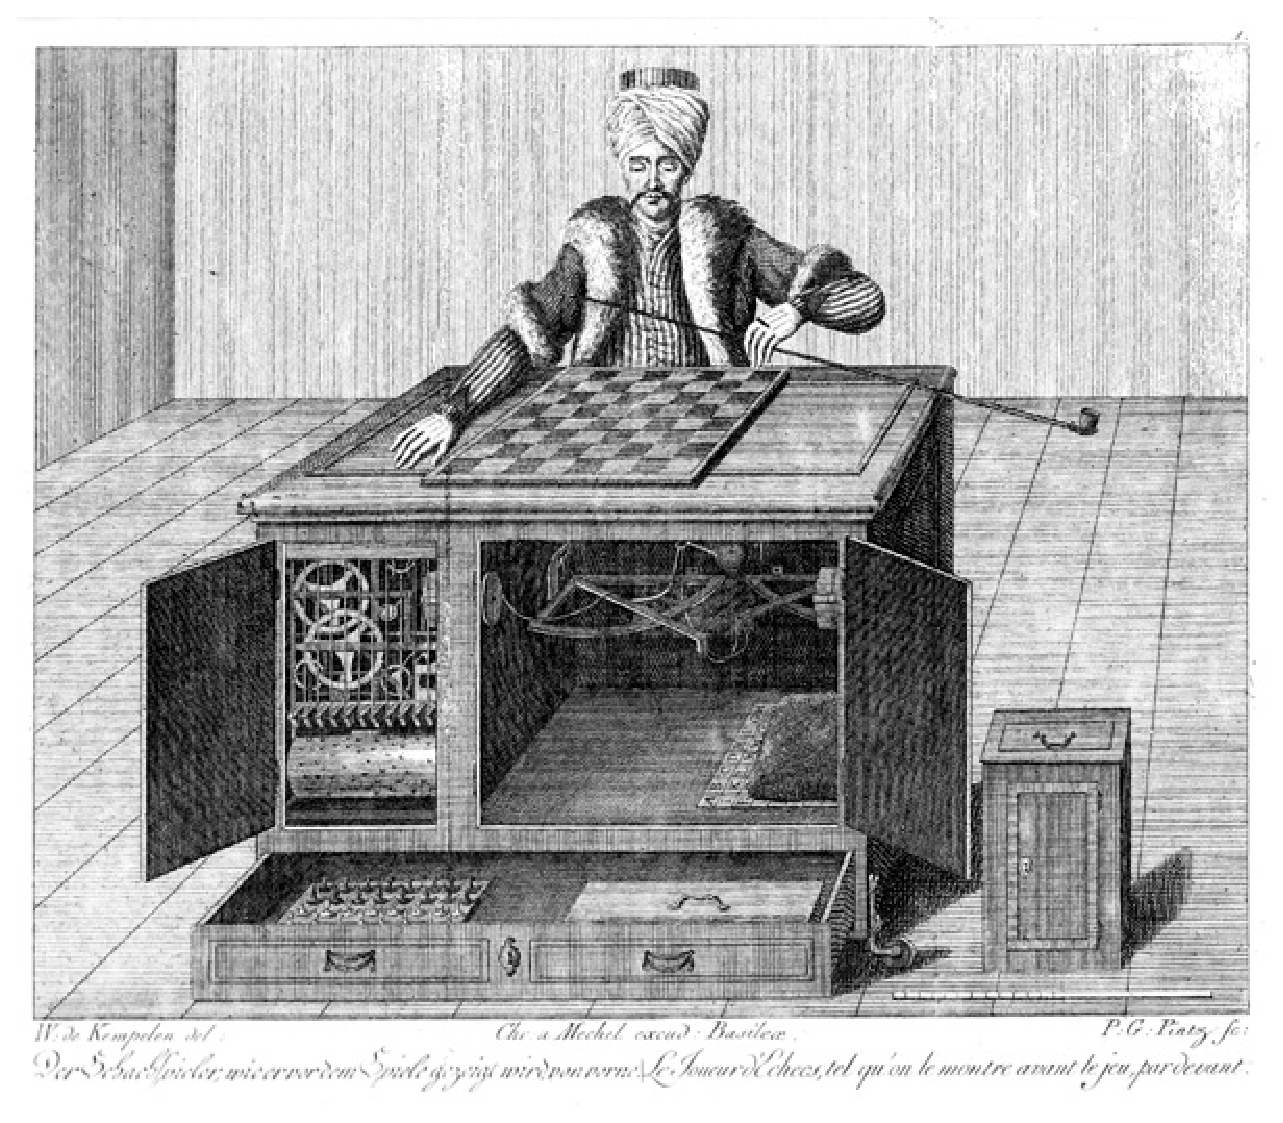
\includegraphics[width=0.75\linewidth]{Figures/mturk.eps}
\end{quoting}

\index{Mechanical Turk}
\tableofcontents

\setcounter{chapter}{-1}
\renewcommand{\thefigure}{\arabic{chapter}.\arabic{figure}}

% Define macros here:
\def\NN{\mathbb{N}}
\def\RN{\mathbb{R}}
\def\ZN{\mathbb{Z}}
\def\IN{\mathbb{I}}
\def\QN{\mathbb{Q}}
\def\EN{\mathbb{E}}
\def\NNN{\mathbb{P}}
\def\<{\text{\textless}}
\def\>{\text{\textgreater}}
\def\cent{\text{\textcent}}
\def\DBAR{\ensuremath{\overline{\delta}}}
\def\PBAR{\ensuremath{\overline{\psi}}}
\def\OBAR{\ensuremath{\overline{\omega}}}
% The following makes a wide bar to overshadow the superscript, too.
\newcommand{\deltabar}[1]{\overline{\delta^{#1}}}
\def\DSIG{\ensuremath{\mathfrak{D}_\Sigma}}
\def\WSIG{\ensuremath{\mathfrak{W}_\Sigma}}
\def\NSIG{\ensuremath{\mathfrak{N}_\Sigma}}
\def\RSIG{\ensuremath{\mathfrak{R}_\Sigma}}
\def\GSIG{\ensuremath{\mathfrak{G}_\Sigma}}
% CSIG is the designator of _C_ontext free languages:
\def\CSIG{\ensuremath{\mathfrak{C}_\Sigma}}
%no such thing as ISIG; after cleanup, the following ISIG line can be removed:
\def\ISIG{\ensuremath{\mathfrak{I}_\Sigma}}
\def\USIG{\ensuremath{\mathfrak{U}_\Sigma}}
\def\XSIG{\ensuremath{\mathfrak{X}_\Sigma}}
\def\PSIG{\ensuremath{\mathfrak{P}_\Sigma}}
\def\FSIG{\ensuremath{\mathfrak{F}_\Sigma}}
% the 'A' is totally unreadable and unintuitive; consider \cal???
\def\ASIG{\ensuremath{\cal{A}_\Sigma}}
%\def\ASIG{\ensuremath{\mathfrak{A}_\Sigma}}
\def\TSIG{\ensuremath{\mathfrak{T}_\Sigma}}
\def\LSIG{\ensuremath{\mathfrak{L}_\Sigma}}
% several of the LSIGs should be ZSIGs
\def\ZSIG{\ensuremath{\mathfrak{Z}_\Sigma}}
\def\OSIG{\ensuremath{\mathfrak{O}_\Sigma}}
\def\HSIG{\ensuremath{\mathfrak{H}_\Sigma}}

%\pagenumbering{arabic} <-- this did not work correctly here; placed just after start of ch-00.tex instead
\chapter{Preliminaries}\label{ch-0}
%\pagenumbering{arabic} % use this only if we revert to roman numerals for the front matter

This chapter reviews some of the basic concepts used in this text. Many can be
found in standard texts on discrete mathematics. Much of the notation employed
in later chapters is also presented here.

\section{Logic and Set Theory}\label{sec-0.1}
A basic familiarity with the nature of formal proofs is assumed; most proofs
given in this text are complete and rigorous, and the reader is encouraged to
work the exercises in similar detail. A knowledge of logic circuits would be
necessary to construct the machines discussed in this text. Important
terminology and techniques are reviewed here.

Unambiguous \emph{statements} that can take on the values {\bf True} or {\bf False} 
(denoted by $1$ and $0$, respectively) can be combined with \emph{connectives} such as
{\em and} ($\wedge$), {\em or} ($\vee$), and {\em not} ($\neg$)
to form more complex statements.
The truth tables for several useful connectives are given in Figure \ref{fig-0.1},
along with the symbols representing the physical devices that implement these
connectives.

As an example of a complex statement, consider the assertion that two statements
$p$ and $q$ take on the same value. This can be rephrased as:
Either ($p$ is true and $q$ is true) or ($p$ is false and $q$ is false).  As the
truth table for {\em not} shows, a statement r is false exactly when $\neg$r is
true; the above assertion could be further refined to:
Either ($p$ is true and $q$ is true) or ($\neg p$ is true and $\neg q$ is true).

% Figure 0.1
\begin{figure}
\begin{center} 
% top of fig0.1 same as fig1.14:
\centerline{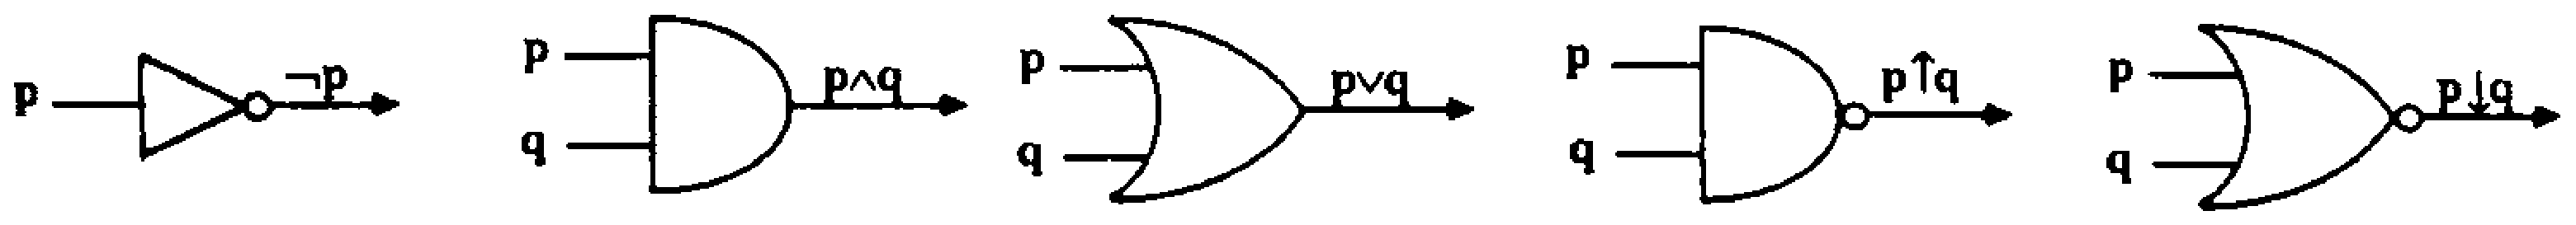
\epsfig{figure=ToFAfigures/fig1-14.eps,width=5.7in}}
\begin{tabular}{ccccc} 
%\fbox{IMAGE} & \fbox{IMAGE} & \fbox{IMAGE} & \fbox{IMAGE} & \fbox{IMAGE} \\ 
NOT gate & AND gate & OR gate & NAND gate & NOR gate \\ 
{ 
\begin{tabular}[b]{c|c} 
$p$ & $\neg p$ \\ 
\hline 
1 & 0 \\ 
0 & 1 
\end{tabular} 
} & { 
\begin{tabular}{cc|c} 
$p$ & $q$ & $p\wedge q$ \\ 
\hline 
1 & 1 & 1 \\ 
1 & 0 & 0 \\ 
0 & 1 & 0 \\ 
0 & 0 & 0 
\end{tabular} 
} & { 
\begin{tabular}{cc|c} 
$p$ & $q$ & $p\vee q$ \\ 
\hline 
1 & 1 & 1 \\ 
1 & 0 & 1 \\ 
0 & 1 & 1 \\ 
0 & 0 & 0 
\end{tabular}
} & { 
\begin{tabular}{cc|c} 
$p$ & $q$ & $p \uparrow q$ \\ 
\hline 
1 & 1 & 0 \\ 
1 & 0 & 1 \\ 
0 & 1 & 1 \\ 
0 & 0 & 1 
\end{tabular} 
} & { 
\begin{tabular}{cc|c} 
$p$ & $q$ & $p \downarrow q$ \\ 
\hline 
1 & 1 & 0 \\ 
1 & 0 & 0 \\ 
0 & 1 & 0 \\ 
0 & 0 & 1 
\end{tabular} 
} 
\end{tabular} 
\end{center}
\caption{Common logic gates and their truth tables}\label{fig-0.1}
\end{figure}


In symbols, this can be abbreviated as:
$$(p \wedge q) \vee (\neg p \wedge \neg q)$$
The truth table covering the four combinations of truth values of $p$ and $q$
can be built from the truth tables defining $\wedge$, $\vee$, and $\neg$, as
shown in \ref{fig-0.2}. The truth table shows that the assertion is indeed
true in the two cases where $p$ and $q$ reflect the same values, and false in
the two cases where the values assigned to $p$ and $q$ differ. When the statement
that $r$ and $s$ always take on the same value is indeed true, we often write
$r$\ {\em iff}\ $s$ (``$r$ if and only if $s$''). The \Index{biconditional} can also be denoted by
$r \Leftrightarrow s$ (``$r$ is \emph{equivalent} to $s$'').\index{equivalent!logical expressions}

% Figure 0.2
\begin{figure}[tb]
\begin{center}
\begin{tabular}{cc|ccccc}
$p$ & $q$ & $\neg p$ & $\neg q$ & $\neg p\wedge\neg q$ & $p\wedge q$ &
	$(p\wedge q)\vee(\neg p\wedge\neg q)$\\
\hline
1 & 1 & 0 & 0 & 0 & 1 & 1\\
1 & 0 & 0 & 1 & 0 & 0 & 0\\
0 & 1 & 1 & 0 & 0 & 0 & 0\\
0 & 0 & 1 & 1 & 1 & 0 & 1
\end{tabular}
\end{center}
\caption{Truth tables for various compound expressions}\label{fig-0.2}
\end{figure}

Consider the statement $(p \wedge q) \vee (p \downarrow q)$.
Truth tables can be constructed to
verify that $(p \wedge q)  \vee (\neg p \wedge \neg q)$ and 
$(p \wedge q) \vee (p \downarrow q)$ have identical truth tables, and
thus $(p \wedge q) \vee (\neg p \wedge \neg q) \Leftrightarrow (p \wedge q)
\vee (p \downarrow q)$.

\subsection*{Example 0.1}

Circuitry for realizing each of the above statements is displayed in Figure
\ref{fig-0.3}. Since the two statements were equivalent, the circuits will
exhibit the same behavior for all combinations of input signals $p$ and $q$.
The second circuit would be less costly to build since it contains fewer
components, and tangible benefits therefore arise when equivalent but less
cumbersome statements can be derived. Techniques for \emph{minimizing} such circuitry
are presented in most discrete mathematics texts.

Example 0.1 shows that it is straightforward to implement statement formulas
by circuitry. Recall that the location of the $1$ values in the truth table can
be used to find the corresponding \emph{\Index{principal disjunctive normal
form}} (\Index{PDNF}) for the expression represented by the truth table. For
example, the truth table corresponding to NAND has three rows with $1$ values
$(p = 1, q = 0; p = 0, q = 1; p = 0, q = 0)$, leading to three \emph{terms} in the PDNF
expression: $(p \wedge \neg q) \vee (\neg p \wedge q) \vee  (\neg p \wedge \neg
q)$. This formula can be implemented as the circuit illustrated in Figure
\ref{fig-0.4} and thus a NAND gate can be replaced by this combination of three
ANDs and one OR gate. This circuit relies on the assurance that a quantity of
interest (such as $p$) will generally be available in both its negated and
unnegated forms. Hence we can count on access to an input line representing
$\neg p$ (rather than feeding the input for $p$ into a NOT gate).

% Figure 0.3
\begin{figure}[tb]
%\centerline{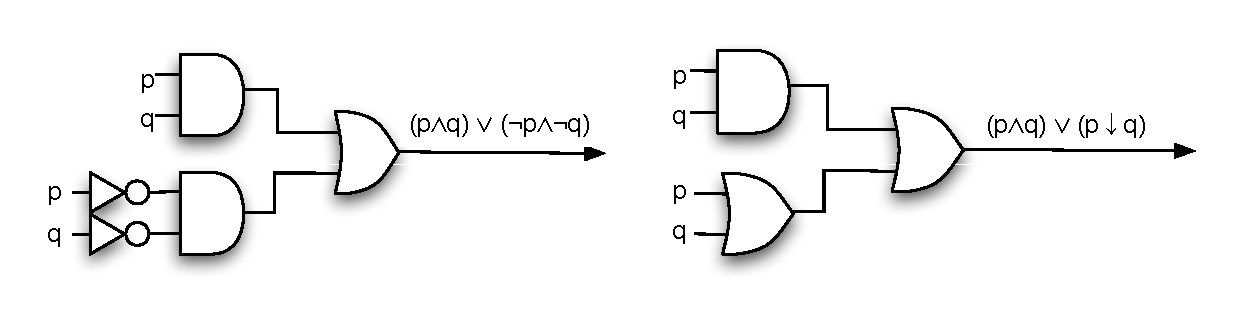
\epsfig{figure=Figures/fig-0-3.eps,width=\textwidth}}
\centerline{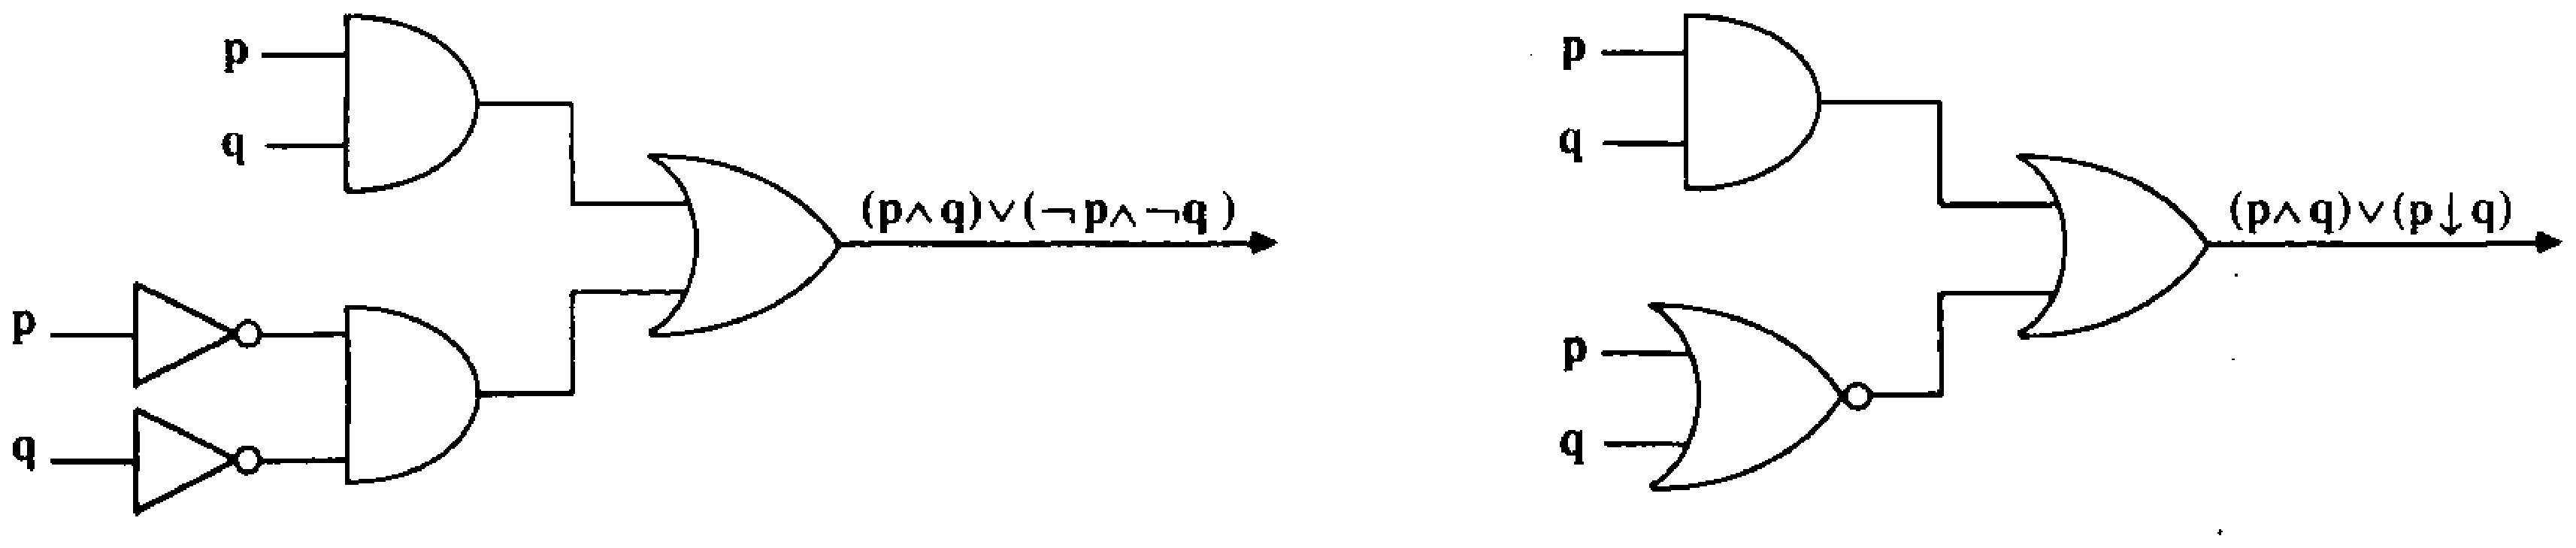
\epsfig{figure=ToFAfigures/fig0-3.eps,width=6.5in}}
\caption{Functionally equivalent circuits}\label{fig-0.3}
\end{figure}

% Figure 0.4
\begin{figure}[tb]
%\centerline{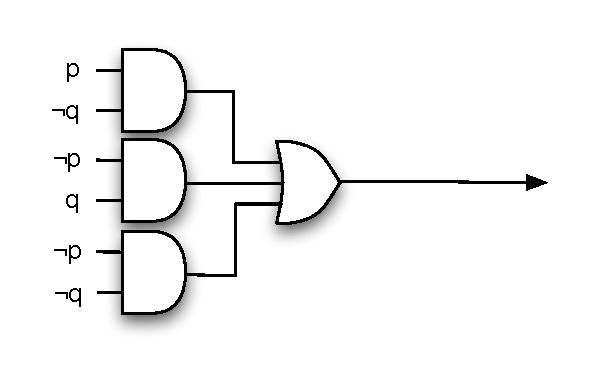
\epsfig{figure=Figures/fig-0-4.eps,width=\textwidth}}
\centerline{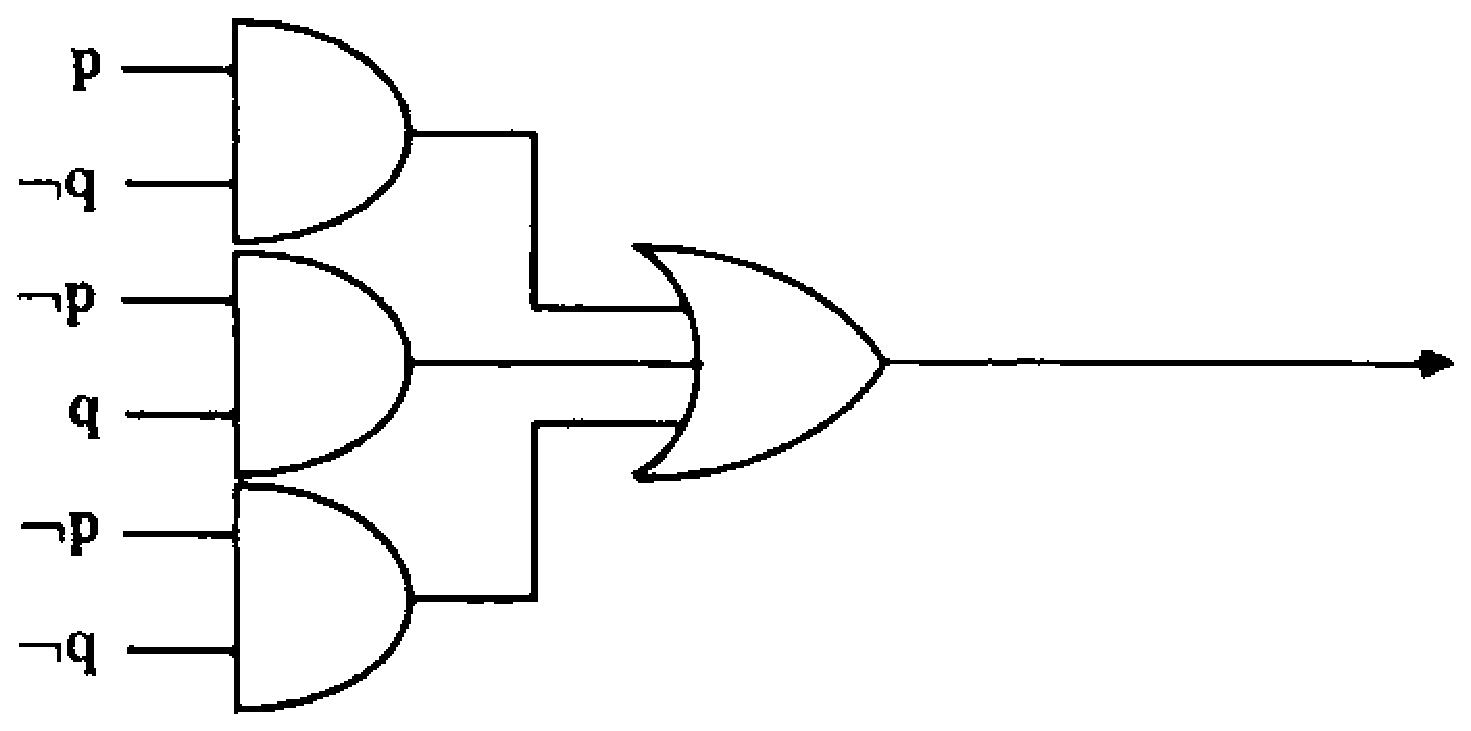
\epsfig{figure=ToFAfigures/fig0-4.eps,width=3.5in}}
\caption{A circuit equivalent to a single NAND gate}\label{fig-0.4}
\end{figure}

In a similar fashion, \emph{any} statement formula can be represented as a group of
AND gates feeding a single OR gate. In larger truth tables, there may
be many more $1$ values, and hence more complex statements may need many AND
gates. Regardless of the statement complexity, however, circuits based on the
PDNF of an expression will allow for a fast response to changing input signals,
since no signal must propagate through more than two gates.

Other useful equivalences are given in Figure \ref{fig-0.5}. Each rule has a \emph{dual}, written
on the same line.\index{associative law}\index{commutative law}\index{absorption law}\index{De Morgan's law}

% Figure 0.5
\begin{figure}[tb]
\begin{tabular}{r@{ $\Leftrightarrow$ }l@{$\qquad$}r@{ $\Leftrightarrow$ }l@{$\qquad$}l}
$(p \vee q) \wedge r$ & $(p \wedge r) \vee (q \wedge r)$ & $(p \wedge q) \vee r$
	& $(p \vee r) \wedge (q \vee r)$ & (distributive laws) \\
$(p \vee q) \vee r$ & $p \vee (q \vee r)$ & $(p \wedge q) \wedge r$ & $p \wedge
	(q \wedge r)$ & (associative laws) \\
$p \vee q$ & $q \vee p$ & $p \wedge q$ & $q \wedge p$ & (commutative laws) \\
$\neg (p \vee q)$ & $\neg p \wedge \neg q$ & $\neg (p \wedge q)$ & $\neg p \vee
	\neg q$ & (De Morgan's laws) \\
$(p \vee q) \wedge p$ & $p$ & $(p \wedge q) \vee p$ & $p$ & (absorption laws) \\
$p \vee \neg p$ & {\bf True} & $p \wedge \neg p$ & {\bf False} & (mutual
	exclusion)
\end{tabular}
\caption{Some useful equivalences and their duals}\label{fig-0.5}
\end{figure}

\emph{Predicates} are often used to make statements about certain \emph{objects}, such as
the numbers in the set ($\ZN$) of integers. For example, $Q$ might represent
the property of being less than 5, in which case $Q(x)$ will represent the
statement ``x is less than 5.'' Thus, $Q(3)$ is true, while $Q(7)$ is false. It
is often necessary to make global statements such as: \emph{All} integers have the
property $P$, which can be denoted by $(\forall x \in \ZN)P(x)$. Note that the
\emph{dummy} variable $x$ was used to state the concept in a convenient form; $x$ is
not meant to represent a particular object, and the statement could be
equivalently phrased as $(\forall i \in \ZN)P(i)$. For the predicate $Q$ defined
above, the statement $(\forall x \in \ZN)Q(x)$ is false, while when applied to
more restricted domains, $(\forall x \in\{1,2,3\})Q(x)$ is true, since it is in
this case equivalent to $Q(1) \wedge Q(2) \wedge Q(3)$, or $(1 < 5) \wedge (2 <
5) \wedge (3<5)$.

In a similar fashion, the statement that \emph{some} integers have the property $P$
will be denoted by $(\exists i\ \in\ \ZN)P(i)$. For the predicate $Q$ defined
above, $(\exists i\ \in \{4, 5, 6\})Q(i)$ is true, since it is equivalent to
$Q(4) \vee Q(5) \vee Q(6)$, or $(4 < 5) \vee (5 < 5) \vee (6 < 5).$ The
statement $(\exists y \in\{7, 8, 9\})Q(y)$ is false.

Note that asserting that it is not the case that all objects have the property
$P$ is equivalent to saying that there is at least one object that does not have
the property $P$. In symbols, we have
$$\neg(\forall x\in\ZN)P(x)\Leftrightarrow(\exists x\in\ZN)(\neg P(x))$$
Similarly,
$$\neg(\exists x\in\ZN)P(x)\Leftrightarrow(\forall x\in\ZN)(\neg P(x))$$
Given two statements $A$ and $B$, if $B$ is true whenever $A$ is true, we will
say that $A$ \emph{implies} $B$, and write $A \Rightarrow B$. For example, the
truth tables show that $p\wedge q\Rightarrow p\vee q$, since for the case where
$p\wedge q$ is true ($p=1,q=1$), $p\vee q$ is true, also. In the cases where $p
\wedge q$ is false, the value of $p\vee q$ is immaterial.

A basic knowledge of set theory is assumed. Some standard special symbols will
be repeatedly used to designate common sets.

% Definition 0.1
\begin{dfn}\label{dfn-0.1}
The set of {\em natural numbers\/} is given by $\NN = \{0,1,2,3,4, \ldots \}$.\index{natural numbers}\index{N @$\NN$|see{natural numbers}}

The set of {\em integers\/} is given by $\ZN =\{\ldots,-2,-1,0,1,2,\ldots\}$.\index{Z @$\ZN$ (integers)}

The set of {\em rational numbers\/} is given by $Q=\{\tfrac{a}{b}\ |\ a\in\ZN\wedge
b\in\ZN\wedge b\neq 0 \}$.\index{Q @$\QN$ (rationals)}

The set of {\em real numbers\/} (points on the number line) will be denoted by
$\RN$.\index{R @$\RN$ (reals)}
\end{dfn}

The following concepts and notation will be used frequently throughout the text.

% Definition 0.2.
\begin{dfn}\label{dfn-0.2}
Let $A$ and $B$ be sets. $A$ is a \emph{\Index{subset}} of $B$ if every element
of $A$ also belongs to $B$; that is, $A \subseteq B \Leftrightarrow (\forall x)
(x \in A \Rightarrow x \in B)$.
\end{dfn}

% Definition 0.3. 
\begin{dfn}\label{dfn-0.3}
Two sets $A$ and $B$ are said to be \emph{\Index{equal}} if they contain exactly
the same elements; that is, $A = B \Leftrightarrow (\forall x)(x \in A
\Leftrightarrow x \in B)$.
\end{dfn}

Thus, two sets $A$ and $B$ are equal \emph{iff} $A \subseteq B$ and $B \subseteq
A$. The symbol $\subset$ will be used to denote a \emph{proper} subset: 
$A \subset B$ \emph{iff} $A \subseteq B$ and $A \neq B$.\index{equality!of sets}

% Definition 0.4.
\begin{dfn}\label{dfn-0.4}
For sets $A$ and $B$, the \emph{\Index{cross product}}\index{Cartesian product|see{cross product}} of $A$ with $B$, is the
set of all ordered pairs from $A$ and $B$; that is, 
$A \times B = \{\langle a, b\rangle \ |\  a \in A \wedge b \in B\}$.
\end{dfn}

\section{Relations}\label{sec-0.2}
Relations are used to describe relationships between members of sets of objects.
Formally, a relation is just a subset of a cross product of two sets.

% Definition 0.5
\begin{dfn}\label{dfn-0.5}
Let $X$ and $Y$ be sets. A relation $R$ from $X$ to $Y$ is simply a
subset of $X \times Y$. If $\langle a,b\rangle \in R$, we write $aRb$. If
$\langle a,b\rangle\notin R$, we write $a$$\not\! R b$. If $X = Y$, we say $R$ is
a relation \underline{\emph{in}} X.
\end{dfn}

\subsection*{Example 0.2}

Let $X = \{1,2,3\}$. The familiar relation $<$ (less than) would then consist of
the following ordered pairs:
$<: \{\langle 1, 2\rangle , \langle 1, 3\rangle , \langle 2, 3\rangle \}$,
by which we mean to indicate that $1 < 2, 1 < 3$, and $2 < 3$.
$\langle 3,3\rangle \notin <$ since $3 \not< 3$.

Some relations have special properties. For example, the relation ``less than''
is \emph{transitive}, by which we mean that for any numbers $x, y,$ and $z,$
if $x < y$ and $y < z$, then $x < z$. Definition \ref{dfn-0.6} describes an important
class of relations that have some familiar properties.

% Definition 0.6
\begin{dfn}\label{dfn-0.6}
A relation is \emph{\Index{reflexive}} iff $(\forall x)(xRx)$.

A relation is \emph{\Index{symmetric}} iff $(\forall x)(\forall y)(xRy
	\Rightarrow yRx)$.

A relation is \emph{\Index{transitive}} iff $(\forall x)(\forall y)(\forall z)
	((xRy \wedge yRz) \Rightarrow x Rz).$
    
An \emph{equivalence relation} is a relation that is reflexive, symmetric, and
transitive.
\end{dfn}

\subsection*{Example 0.3}

\< is not an equivalence relation; while it is transitive, it is not reflexive
since $3 \not< 3$. (It is also not symmetric, since $2 < 3$, but $3 \not< 2$.)

\subsection*{Example 0.4}

Let $X = \NN$. The familiar relation $=$ (equality) \emph{is} an equivalence
relation.
$$= :\{\langle 0, 0\rangle , \langle 1,1\rangle , \langle 2,2\rangle ,
	\langle 3,3\rangle , \langle 4,4\rangle , \ldots \},$$
and it is clear that $(\forall x)(\forall y)(x = y \Rightarrow y = x)$.
The equality relation is therefore symmetric, and it is likewise obvious that
$=$ is also reflexive and transitive.

% Definition 0.7
\begin{dfn}\label{dfn-0.7}
Let $R$ be an equivalence relation in $X$, and let $h \in X$. Then $[h]_R$
refers to the \emph{equivalence class} consisting of all entities that are
related to $h$ by the equivalence relation $R$; that is, $[h]_R = \{y\ |\ y\ R\ h\}$.
\end{dfn}

\subsection*{Example 0.5}

The equivalence classes for $=$ are singleton sets: $[1]_==\{1\},[5]_==\{5\}$,
and so on.

\subsection*{Example 0.6}

Let $X = \ZN$, and define the relation $R$ in $\ZN\times\ZN$ by

$$\langle u, v\rangle R\langle w,x\rangle\ \text{{\em iff}}\ ux = vw$$

If $\langle x, y\rangle$ is viewed as the fraction $\frac{x}{y}$, then $R$ is
the relation that identifies equivalent fractions: $\frac{2}{3}R\frac{14}{21}$,
since $2\cdot 21=3\cdot 14$. In this sense, $R$ can be viewed as the \emph{equality}
operator on the set of rational numbers~$\QN$.\index{equality!of rationals}

Note that in this context the equivalence class $[\frac{2}{8}]_R$ represents the
set of all ``names'' for the point one-fourth of the way between $0$ and $1$;
that is,
$$\left[\frac{2}{8}\right]_R = \{\ldots ,\frac{-3}{-12}, \frac{-2}{-8},
\frac{-1}{-4}, \frac{1}{4},\frac{2}{8},\frac{3}{12},\frac{4}{16},\frac{5}{20},
\ldots \}$$
There are therefore many other ways of designating this same set; for example,
$$\left[\frac{1}{4}\right]_R = \{ \ldots , \frac{-3}{-12}, \frac{-2}{-8}, \frac{-1}{-4},
    \frac{1}{4},\frac{2}{8},\frac{3}{12},\frac{4}{16},\frac{5}{20}, \ldots \}$$

\subsection*{Example 0.7}

Let $X = \NN$ and choose an $n \in \NN$. Define $R_n$ by
$$x R_n y \text{\em { iff }}\, \, (\exists i \in \ZN)(x - y = i\cdot n)$$
That is, two numbers are related if their difference is a multiple of $n$.
Equivalently, $x$ and $y$ must have the same remainder upon dividing each of
them by $n$ if we are to have $x R_n y$
.
$R_n$ can be shown to be an equivalence relation for each natural number $n$.
The equivalence classes of $R_2$, for example, are the two familiar sets, the
even numbers and the odd numbers. The equivalence classes for $R_3$ are
\begin{center}\begin{tabular}{r@{ $=$ }l}
$[0]_{R_3}$ & $\{0, 3, 6, 9, 12, 15, \ldots \}$ \\
$[1]_{R_3}$ & $\{1, 4,7,10,13, \ldots \}$ \\
$[2]_{R_3}$ & $\{2, 5, 8,11,14, \ldots \}$
\end{tabular}\end{center}

$R_n$ is often called \emph{\Index{congruence modulo $n$}}, and $x R_n\!y$ is
commonly denoted by $x \equiv y\!\pmod{ n}$ or $x \equiv _n$$y$.

If $R$ is an equivalence relation in $X$, then every element of $X$ belongs to
exactly one equivalence class of $R$. $X$ is therefore comprised of the union of
the equivalence classes of $R$, and in this sense $R$ \emph{partitions} the set
$X$ into disjoint subsets. Conversely, a partition of $X$ defines an equivalence
relation in $X$; the sets of the partition can be thought of as the equivalence
classes of the resulting relation.

% Definition 0.8
\begin{dfn}\label{dfn-0.8}
Given a set $X$ and sets
$A_1 , A_2 , \ldots , A_n ,$ the collection $P = \{A_1 ,A_2 , \ldots ,A_n \}$
is a \emph{partition} of $X$ if the sets in $P$ are all \emph{subsets} of $X$,
they \emph{cover} $X$, and are \emph{pairwise disjoint}. That is, the following
three conditions are satisfied:

\begin{tabular}{r@{ $\in$ }l}
$(\forall i$ & $\{1,2, \ldots ,n\})(A_i \subseteq X)$ \\
$(\forall x$ & $X)(\exists i \in \{1,2, \ldots ,n\} \ni x \in A_i )$ \\
$(\forall i,j$ & $\{1, 2, \ldots ,n\})(i \not= j \Rightarrow A_i \cap A_j = \emptyset)$
\end{tabular}
\end{dfn}

% Definition 0.9
\begin{dfn}\label{dfn-0.9}
Given a set $X$ and a partition $P = \{A_1,A_2, \ldots ,A_n \}$ of $X$,
the relation $R(P)$ in $X$ induced by $P$ is given by
$$(\forall x \in X)(\forall y \in X)(x \, R(P) \, y \Leftrightarrow
  (\exists i \in \{1,2, \ldots ,n\} \ni x \in A_i \wedge y\in A_i))$$
\end{dfn}

$R(P)$ thus relates elements that belong to the same subset of $P$.

\subsection*{Example 0.8}

Let $X = \{1, 2, 3, 4, 5\}$ and consider the relation $Q = R(S)$ induced by the
partition $S = \{\langle 1, 2\rangle,\langle 3, 5\rangle,\langle 4\rangle\}$.
Since 1 and 2 are in the same set, they should be related by $Q$, while
$1$$\not\!\!\!Q 4$ because $1$ and $4$ belong to different sets of the partition.
Q can be described by
$$ Q = \{\langle 1, 1\rangle, \langle 1,2\rangle, \langle 2, 1\rangle,
\langle 2,2\rangle, \langle 3,3\rangle, \langle 3, 5\rangle,
\langle 4, 4\rangle, \langle 5, 3\rangle, \langle 5, 5\rangle\} $$

It is straightforward to check that $Q$ satisfies the three properties needed to
qualify as an equivalence relation, and the equivalence classes of $Q$ are
\begin{center}\begin{tabular}{r@{ $=$ }l}
$[1]_Q$ & $\{1,2\}$ \\
$[2]_Q$ & $\{1,2\}$ \\
$[3]_Q$ & $\{3,5\}$ \\
$[4]_Q$ & $\{4\}$ \\
$[5]_Q$ & $\{3,5\}$
\end{tabular}\end{center}

The set of \emph{distinct} equivalence classes of $Q$ can be used to partition
$X$; note that these three classes comprise $S$. In a similar manner, the three
distinct equivalence classes of $R_3$ in Example 0.7 form a partition of $\NN$.

A ``finer'' partition of $X$ can be obtained by breaking up the equivalence
classes of $Q$ into smaller (and hence more numerous) sets. The resulting
relation is called a \emph{refinement} of $Q$.

% Definition 0.10
\begin{dfn}\label{dfn-0.10}
Given two equivalence relations $R$ and $Q$ in a set $X$, $R$ is a
\emph{\Index{refinement}} of $Q\text{ iff }R \subseteq Q$; that is,
$(\forall x \in X)(\forall y \in X)(\langle x,y\rangle  \in R \Rightarrow \langle x,y\rangle  \in Q).$
\end{dfn}

\subsection*{Example 0.9}

Consider $Q = \{\langle 1, 1\rangle, \langle 1,2\rangle, \langle 2,1\rangle,
\langle 2,2\rangle, \langle 3,3\rangle, \langle 3,5\rangle, \langle 4,4\rangle,
\langle 5,3\rangle, \langle 5,5\rangle\}$
and $S =\{\langle 1, 1\rangle, \langle 2,2\rangle, \langle 3,3\rangle, \\
\langle 3,5\rangle, \langle 4,4\rangle, \langle 5,3\rangle,
\langle 5, 5\rangle\}$. $S$ is clearly a subset of $Q$, and hence $S$ refines
$Q$. Note that the partition induced by $S, \{\{1\}, \{2\}, \{3,5\},\{4\}\}$,
indeed splits up the partition induced by $Q$, which was
$\{\{1,2\},\{3,5\}, \{4\}\}$. While it may at first seem strange, the fact that
$S$ contained \emph{fewer} ordered pairs than $Q$ guarantees that $S$ will yield 
\emph{more} equivalence classes than $Q$.

\section{Functions}\label{sec-0.3}

A \emph{function} $f$ is a special type of relation in which each first
coordinate is associated with one and only one second coordinate, in which case
we can use functional notation $f(x)$ to indicate the unique element $f$
associates with a given first coordinate $x$. In the previous section we
concentrated on relations \emph{in} $X$, that is, subsets of $X \times X$. The
set of first coordinates of a function $f$ (the \emph{domain} $X$) is often
different from the set of possible second coordinates (the \emph{codomain} $Y$),
and hence $f$ will be a subset of $X \times Y$.

% Definition 0.11
\begin{dfn}\label{dfn-0.11}
A \emph{\Index{function}} f: $X \rightarrow Y$ is a subset of $X \times Y$ for
which 
\begin{enumerate}
\item $(\forall x \in X)(\exists y \in Y \ni xfy)$.
\item $(\forall x \in X)((xfy_1 \wedge xfy_2) \Rightarrow y_1 = y_2 )$.
\end{enumerate}
\end{dfn}

When a pair of elements are related by a function, we will write $f(a) = b$
instead of $afb$ or $\langle a,b\rangle\in f$. The criteria for being a function
could then be rephrased as $(\forall x \in X)(\exists y \in Y \ni f(x) = y)$,
and $(\forall x_1 \in X)(\forall x_2 \in X)(x_1 = x_2
\Rightarrow f(x_1) = f(x_2))$.

\subsection*{Example 0.10}

Let $n$ be a positive integer. Define $f_n$: $\NN \rightarrow \NN$ by $f_{n}(j)
=$ the smallest natural number $i$ for which $j \equiv i \bmod{n}, f_3 (j)$,
for example, is a function and is represented by the ordered pairs
$f_3: \{\langle 0, 0\rangle, \langle 1, 1\rangle, \langle 2, 2\rangle,
\langle 3, 0\rangle, \\ \langle 4,1\rangle, \ldots \}$. This implies that
$f_3 (0) = 0$, $f_3 (1) = 1$, $f_3 (2) = 2$, $f_3 (3) = 0$, and so on.

Note that $f_3$ is a subset of the relation $R_3$ given in Example 0.7. If $R_3$
were presented as a function, it would not be {\em well defined}; that is, $R_3$
does not satisfy Definition \ref{dfn-0.11}. For example, $2 R_3 5$ and $2 R_3 8$, but
$5 \not= 8$, and so $R_3 (2)$ is not a meaningful expression, since there is no
unique object that $R_3$ associates with 2. In this case, $R_3$ violated 
Definition \ref{dfn-0.11} by associating \emph{more} than one object with a
given first coordinate; in general, a proposed relation may also fail to be well
defined by associating \emph{no} objects with a potential first coordinate.

\subsection*{Example 0.11}

Consider the ``function'' $g$: $\QN \rightarrow \NN$ defined by $g(\frac{m}{n})
=m$. This apparently straightforward definition is fundamentally flawed.
According to the formula, $g\left(\frac{2}{8}\right)=2$, $g\left(\frac{7}{9}
\right)=7$, $g\left(\frac{5}{10}\right)=5$, and so forth. However, $\frac{2}{8}
=\frac{5}{20}$, but $g\left(\frac{2}{8}\right)=2\not=5=g\left(\frac{5}{20}
\right)$, and Definition \ref{dfn-0.11} is again violated; $g(0.25)$ is not a
well defined quantity, and thus the ``function'' $g$ is not well defined. Had
$g$ truly been a function, it would have passed the test: if $x=y$, then $g(x)=
g(y)$.

The problem with this seemingly innocent definition
is that the domain element 0.25 is actually
an {\em equivalence class} of fractions (recall Example 0.6), and the definition
of $g$ was based on just one \emph{representative} of that class. We observed
that two representatives ($\frac{2}{8}$ and $\frac{5}{20}$) of the \emph{same}
class gave conflicting answers (2 and 5) for the value that $g$ associated with
their class (0.25). While it is possible to define functions on a set of
equivalence classes in a consistent manner, it will always be important to
verify that such functions are {\em single valued}.

Selection criteria, which determine whether a candidate does or does not
belong to a given set, are special types of functions.

% Definition 0.12
\begin{dfn}\label{dfn-0.12}
Given a set $A$, the {\em characteristic function} $\chi_A$ associated with $A$
is defined by
$$\chi_{A}(x)=1\text{ if }x\in A\quad\text{and}\quad\chi_{A}(x)=0\text{ if }x
	\notin A$$
\end{dfn}

\subsection*{Example 0.12}

The characteristic function for the set of odd numbers is the function $f_2$
given in Example 0.10.

To say that a \emph{set} is well defined essentially means that the
characteristic function associated with that set is a well-defined function. A
set of equivalence classes can be ill defined if the definition is based on the
representatives of those equivalence classes.

\subsection*{Example 0.13}

Consider the ``set'' of fractions that have odd numerators, whose characteristic
``function'' is defined by:
$$\chi_{B}\left(\frac{m}{n}\right) = 1\text{ if $m$ is odd}$$
and
$$\chi_{B}\left(\frac{m}{n}\right) = 0\text{ if $m$ is even}$$

This characteristic function suffers from flaws similar to those found in the
function $g$ in Example 0.11. $\frac{1}{4} = \frac{2}{8}$ and yet
$X_B \left(\frac{1}{4}\right) = 1$ while $X_B \left(\frac{2}{8}\right) = 0$,
which implies that the fraction $\frac{1}{4}$ belongs to $B$, while
$\frac{2}{8}$ is not an element of $B$. Due to this ambiguous definition of set
membership, $B$ is not a well-defined set. $B$ failed to pass the test: if
$x = y$, then $(x \in B$ \emph{iff} $y\in B)$.

The definition of a relation requires the specification of the domain, codomain,
and the ordered pairs comprising the relation. For relations that are functions,
every domain element must occur as a first coordinate. However, the set of
elements that occur as second coordinates need not include all the codomain
(as was the case in the function $f_n$ in Example 0.10).

% Definition 0.13
\begin{dfn}\label{dfn-0.13}
The \emph{\Index{range}} of a function $f: X \rightarrow Y$ is given by
$$\{y \in Y\ |\  \exists x \in X \ni f(x) = y\}$$
\end{dfn}

Conditions similar to those imposed on the behavior of first coordinates of a
function may also be placed on second coordinates, yielding specialized types
of functions. Functions for which the range encompasses all the codomain, for
example, are called \emph{surjective}

% Definition 0.14
\begin{dfn}\label{dfn-0.14}
A function $f$: $X \rightarrow Y$ is \emph{\Index{onto}} or
\emph{\Index{surjective}} iff
$$(\forall y \in Y)(\exists x \in X \ni  f(x) = y)\text{; that is,}$$
a set of ordered pairs representing an \emph{onto} function must have at least
one first coordinate associated with any given second coordinate .
\end{dfn}

\subsection*{Example 0.14}

The function $g$: $\{1,2,3\}\rightarrow\{a,b\}$ defined by $g(1) = a$,
$g(2) = b$, and $g(3) = a$ is onto since both codomain elements are part of the
range of $g$. However, the function $h$: $\{1, 2, 3\}\rightarrow \{a, b, c\}$
defined by $h(1) = a$, $h(2) = b$, and $h(3) = a$ is \emph{not} onto since no domain
element maps to $c$.

The function $f$: $\NN \rightarrow \NN$ defined by $f(i)=i+1$ $(\forall i=0,1,2,
\ldots)$ is \emph{not} onto since there is no element $x$ for which $f(x)=0$.

% Definition 0.15
\begin{dfn}\label{dfn-0.15}
A function $f$: $X \rightarrow Y$ is \emph{\Index{one to one}} or
\emph{\Index{injective}} iff
$$(\forall x_1 \in X)(\forall x_2 \in X)(f(x_1) = f(x_2)
	\Rightarrow x_1 = x_2)\text{; that is,}$$
an \emph{injective} function must not have more than one first coordinate
associated with any given second coordinate .
\end{dfn}

\subsection*{Example 0.15}

The function $f$: $\NN \rightarrow \NN$ defined by $f(i)=i+1$ $(\forall i=0,1,2,
\ldots)$ is clearly injective since if $f(i)= f(j)$ then $i+1=j+1$, and so $i$
must equal $j$.

The function $g$: $\{1,2,3\}\times\{a,b\}$ defined by $g(1)=a$, $g(2)=b$,
and $g(3)=a$ is not one to one since $g(1)=g(3)$, but $1\not= 3$.

% Definition 0.16
\begin{dfn}\label{dfn-0.16}
A function is a \emph{\Index{bijection}} iff it is one to one and onto
(injective and surjective); that is, it must satisfy
\begin{enumerate}
\item $(\forall x_1 \in X)(\forall x_2 \in X)(f(x_1) = f(x_2) \Rightarrow x_1 =
	x_2)$.
\item $(\forall y \in Y)(\exists x \in X \ni f(x) = y)$.
\end{enumerate}
\end{dfn}

A \emph{bijective} function must therefore have \emph{exactly} one first
coordinate associated with any given second coordinate.

\subsection*{Example 0.16}

The function $f$: $\NN \rightarrow \NN$ defined by $f(i)=i+1$ $(\forall i=0,1,2,
\ldots)$ is injective but not surjective, so it is not a bijection. However, the
function $b$: $\ZN\rightarrow\ZN$ defined by $b(i)=i+1$ $(\forall i=\ldots,-2,
-1,0,1,2,\ldots)$ is a bijection. Note that while the rule for $b$ remains the
same as for $f$, both the domain and range have been expanded, and many more
ordered pairs have been added to form the function $b$.

It is often appropriate to take the results produced by one function and apply
the rule specified by a second function. For example, we may have a list
associating students with their height in inches (that is, we have a function
relating names with numbers). The conversion rule for changing inches into
centimeters is also a function (associating any given number of inches with the
corresponding length in centimeters), which can be applied to the heights given
in the student list to produce a new list matching student names with their
height in centimeters. This new list is referred to as the
\emph{\Index{composition}} of the original two functions.

% Definition 0.17
\begin{dfn}\label{dfn-0.17}
The \emph{\Index{composition}} of two functions $f$: $X\rightarrow Y$ and
$g$: $Y\rightarrow Z$ is given by
$$g \circ f = \{\langle x,z\rangle \ |\  \exists y \in Y \ni
	\langle x,y\rangle \in f\text{ and }\langle y,z\rangle \in g\}$$
\end{dfn}

Note that the composition is not defined unless the codomain of the first
function matches the domain of the second function. In functional notation,
$g\circ f=\{\langle x,z\rangle\ |\ \exists y\in Y\ni f(x)=y\text{ and }g(y)=z\}$,
and therefore when $g\circ f$ is defined, it can be described by the rule
$g\circ f(x)=g(f(x))$.

\subsection*{Example 0.17}

Consider the functions $f_3$ from Example 0.10 and $f$ from Example 0.14, where
$f_3$: $\NN\rightarrow\NN$ was defined by $f_3(i) =$ the smallest natural number
$i$ for which $j = i \bmod{3}$, and the function $f$: $\NN\rightarrow\NN$ is
defined by $f(i) = i + 1$. $f \circ f_3$ consists of the ordered pairs
$\{\langle 0,1\rangle,\langle 1,2\rangle,\langle 2,3\rangle,\langle 3,1\rangle,
\langle 4,2\rangle,\langle 5,3\rangle, \ldots \}$ and is represented by the rule
$f\circ f_3(j) = f_3(j) + 1$, which happens to be the smallest {\em positive}
number that is congruent to $j + 1 \bmod{3}$. Note that
$f_3 \circ f(j) = f_3 (j + 1)$, which happens to be the smallest \emph{natural}
number that is congruent to $j + 1 \bmod{3}$. This represents a different set
of ordered pairs $\{\langle 0,1\rangle,\langle 1,2\rangle,\langle 2,0\rangle,
\langle 3,1\rangle,\langle 4,2\rangle,\langle 5,0\rangle, \ldots \}$. In most
cases, $f \circ g \not= g \circ f$.

% Theorem 0.1
\begin{thm}\label{thm-0.1}
Let the functions $f$: $X\rightarrow Y$ and $g$: $Y\rightarrow Z$ be onto. Then
$g\circ f$ is onto.

\emph{Proof.} See the exercises.
\end{thm}

% Theorem 0.2
\begin{thm}\label{thm-0.2}
Let the functions $f$: $X\rightarrow Y$ and $g$: $Y\rightarrow Z$ be one to one.
Then $g\circ f$ is one to one.

\emph{Proof.} See the exercises.
\end{thm}

% Definition 0.18
\begin{dfn}\label{dfn-0.18}
The \emph{\Index{converse}} of a relation $R$, written $\sim\! R$, is defined by
$$\sim\! R = \{\langle y,x\rangle \ |\  \langle x,y\rangle \in R\}$$
The converse of a function $f$ is likewise
$$\sim\!\! f = \{\langle y,x\rangle \ |\  \langle x,y\rangle \in f\}$$
If $\sim\!\! f$ happens to be a function, it is called the \emph{inverse} of $f$ and
is denoted by $f^{-1}$.
\end{dfn}

When the inverse exists, it is appropriate to use functional notation $f^{-1}$
also, and we therefore have, for any elements $a$ and $b$, $f^{-1}(b) = a$
{\em iff} $f(a) = b$. Note that if $f: X \rightarrow Y$ then
$f^{-1}: Y \rightarrow X$.

\subsection*{Example 0.18}

Consider the ordered pairs for the relation
$<: \{\langle 1,2\rangle,\langle 1,3\rangle,\langle 2,3\rangle\}$. The converse
is then $\sim <: \{\langle 2,1\rangle,\langle 3,1\rangle,\langle 3,2\rangle \}$.
Thus, the converse of ``less than'' is the relation ``greater than''

The function $b$:$\ZN \rightarrow \ZN$ defined by
$b(i) = i + 1 (\forall i = \ldots,-2, -1,0,1,2, \ldots)$ has the inverse
$b^{-1}: \ZN \rightarrow \ZN$ defined by
$b^{-1}(i) = i - 1 (\forall i = \ldots,-2,-1,0,1,2,\ldots)$. The inverse of the
function that increments integers by 1 is the function that decrements integers
by the same amount.

The function $f$: $\ZN \rightarrow \ZN$ defined by
$f(i) = i^2 (\forall i = \ldots,-2,-1,0,1,2,\ldots)$ has a converse that is not
a function over the given domain and codomain; the inverse notation is
inappropriate, since $f^{-1}(3)$ is not defined, nor is $f^{-1}(-4)$.

Not surprisingly, if the converse of $f$ is to be a function, the codomain of
$f$ (which will be the new domain of $f^{-1}$) must satisfy conditions similar
to those imposed on the domain of $f$. In particular:

% Theorem 0.3
\begin{thm}\label{thm-0.3}
Let $f$: $X\rightarrow Y$ be a function. The converse of $f$ is a function iff
$f$ is a bijection.

\emph{Proof}. See the exercises.
\end{thm}

If $f$ is a bijection, $f^{-1}$ must exist and will also be a bijection. In
fact, the compositions $f \circ f^{-1}$ and $f^{-1} \circ f$ are the
\emph{identity} functions on the domain and codomain, respectively (see the
exercises).

\section{Cardinality and Induction}\label{sec-0.4}

The \emph{size} of various sets will frequently be of interest in the topics
covered in this text, and it will occasionally be necessary to consider the set
of all subsets of a given set.

% Definition 0.19
\begin{dfn}\label{dfn-0.19}
Given a set $A$, the \emph{\Index{power set}} of $A$, denoted by $\wp (A)$ or
$2^A$, is $$\wp(A) = \{X\ |\ X \subseteq A\}$$
\end{dfn}

\subsection*{Example 0.19}

$$\wp(\{a,b,c\}) =
	\{\emptyset,\{a\},\{b\},\{c\},\{a,b\},\{a,c\},\{b,c\},\{a,b,c\}\}$$
and
$$\wp(\{\ \ \})=\{\emptyset\}.$$
Note that $\{\emptyset\} \not= \emptyset$.

% Definition 0.20
\begin{dfn}\label{dfn-0.20}
Two sets $X$ and $Y$ are \emph{\Index{equipotent}} if there exists a bijection
$f$: $X \rightarrow Y$, and we will write $\| X\| = \| Y\|.\ \ \| X\|$ denotes the
\emph{\Index{cardinality}} of $X$, that is, the number of elements in $X$.
\end{dfn}

That is, sets with the same cardinality or ``size'' are equipotent. The
equipotent relation is reflexive, symmetric, and transitive and is therefore an
equivalence relation.

\subsection*{Example 0.20}

The function $g$: $\{a,b,c\}\rightarrow\{x,y,z\}$ defined by $g(a)=z$, $g(b)=y$,
and $g(c)=x$ is a bijection, and thus $\|\{a,b,c\}\|=\|\{x,y,z\}\|$. The
equivalence class consisting of all sets that are equipotent to $\{a,b,c\}$ is
generally associated with the \emph{cardinal number} 3. Thus, $\|\{a,b,c\}\| =
3$; $\|\{\ \ \}\|=0$. $\{a,b,c\}$ is not equipotent to $\{\ \ \}$, and hence $3
\not= 0$.

The subset relation allows the sizes of sets to be \emph{ordered}:
$\|A\| \leq \|B\|$ {\em iff} $(\exists C)(C \subseteq B \wedge \|A\| = \|C\|)$.
We will write 
$\|A\| < \|B\|$ {\em iff} $(\|A\| \leq \|B\|\text{ and }\|A\| \not= \|B\|)$.
The observations about $\{a,b,c\}$ and $\{\ \}$ imply that $0 < 3$.

For $\NN =\{0,1,2,3,4,5,6, \ldots \}$ and $\EN =\{0,2,4,6, \ldots \}$, the
function $f$: $\NN \rightarrow \EN$, defined by $f(x) = 2x$, is a bijection. The
set of natural numbers $\NN$ is \emph{countably infinite}, and its size is often
denoted by $\aleph_0= \|\NN\|$. The doubling function $f$ shows that
$\|\NN\| = \|\EN\|$. Similarly, it can be shown that $\ZN$ and $\NN \times \NN$
are also countably infinite (see the exercises). A set that is equipotent to one
of its {\em proper} subsets is called an infinite set. Since $\|\NN\| = \|\EN\|$ and
yet $\EN \subset \NN$, we know that $\NN$ must be infinite. No such
correspondence between $\{a,b,c\}$ and any of its proper subsets is possible, so
$\{a,b,c\}$ is a finite set. 3 is therefore a finite cardinal number, while
$\aleph_0$ represents an infinite cardinal number.

Theorem \ref{thm-0.4} compares the size of a set $A$ with the number of subsets of $A$ and
shows that $\|A\| < \|\wp(A)\|$. For the sets in Example 0.19, we see that
$3 < 8$ and $0 < 1$, which is not unexpected. It is perhaps surprising to find
that the theorem will also apply to infinite sets, for example,
$\|\NN\| < \|\wp(\NN)\|$. This means that there are cardinal numbers larger
than $\aleph_0$; there are infinite sets that are not countably infinite.
Indeed, the next theorem implies that there is an unending progression of
infinite cardinal numbers.

% Theorem 0.4
\begin{thm}\label{thm-0.4}
Let A be \emph{any} set. Then $\|A\| < \|\wp(A)\|$

\emph{Proof}. There is a bijection between $A$ and the set of all singleton
subsets of $A$, as shown by the function $s$: $A \rightarrow \{\{x\}\ |\ x \in A\}$
defined by $s(z) = \{z\}$ for each $z \in A$. Since
$\{\{x\}\ |\ x\in A\}\subseteq \wp(A)$, we have $\|A\| \leq \|\wp(A)\|$. It
remains to show that $\|A\| \not= \|\wp(A)\|$. By definition of cardinality, we
must show that there cannot exist a bijection between $A$ and $\wp(A)$. The
following proof by contradiction will show this.

Assume $f$: $A\rightarrow \wp(A)$ is a function; we will demonstrate that there
must exist a set in $\wp(A)$ that is not in the range of $f$, and hence $f$
cannot be onto. Consider an element $z$ of $A$ and the set $f(z)$ to which it
maps. $f(z)$ is a subset of $A$, and hence $z$ may or may not belong to $f(z)$.
Define $B$ to be the set $\{y \in A \ |\  y \notin f(y)\}$. $B$ is then the set of
all elements of $A$ that do not appear in the set corresponding to their image
under $f$. It is impossible for $B$ to be in the range of $f$, for if it were
then there would be an element of $A$ that maps to this subset: assume $w \in A$
and $f(w) = B$. Since $w$ is an element of $A$, it might belong to $B$, which is
a subset of $A$. If $w \in B$, then $w \in f(w)$, since $f(w) = B$; but the
elements for which $y \in f(y)$ were exactly the ones omitted from $B$, and thus
we would have $w \notin B$, which is a contradiction. Our speculation that $w$
might belong to $B$ is therefore incorrect. The only other option is that $w$
does not belong to $B$. But if $w \notin B = f(w)$, then $w$ is one of the
elements that are supposed to be in $B$ and we are again faced with the
impossibility that $w \notin B$ and $w \in B$. In all cases, we reach a
contradiction if we assume that there exists an element $w$ for which $f(w) = B$.
Thus, $B$ was a member of the codomain that is not in the range of $f$, and $f$ 
is therefore not a bijection.
\end{thm}

Sets that are finite or are countably infinite are called
\emph{\Index{countable}} or \emph{\Index{denumerable}} because their elements can be
arranged one after the other (enumerated). We will often need to prove that a
given statement is true in an infinite variety of cases that can be enumerated
by the natural numbers $0,1,2,\ldots$. The assertion that the sum of the first
$n$ positive numbers can be predicted by multiplying $n$ by the number one
larger than $n$ and dividing the result by 2 seems to be true for various test
values of $n$:
\begin{center}\begin{tabular}{r@{ $=$ }l}
$1+2+3$ & $\frac{(3+1)3}{2}$ \\
$1+2+3+4+5$ & $\frac{(5+1)5}{2}$
\end{tabular}\end{center}
and so on. We would like to show that the assertion is true for all values of
$n = 1,2,3, \ldots$, but we clearly could never check the arithmetic
individually for an infinite number of cases. The assertion, which varies
according to the particular number $n$ we choose, can be represented by the
statement
$$P(n)\text{:}\ 1+2+3+\cdots+(n-2)+(n-1)+n\text{ adds up to }\frac{(n+1)n}{2}.$$
Note that $P(n)$ is \emph{not} a number; it is the assertion that two numbers are the
same and therefore will only take on the values {\bf True} and {\bf False}. We
would like to show that $P(n)$ is true for each positive integer $n$; that is,
$(\forall n)P(n)$. Notice that if you were to attempt to check out whether
$P(101)$ was true your work would be considerably simplified if you already knew
how the first 100 numbers added up. If the first 100 summed to 5050, it is clear
that $1+2+\cdots+99+100+101=(1+2+\cdots+99+100)+101=5050+101=5151$; the hard
part of the calculation can be done \emph{without} doing arithmetic with 101
separate numbers. Checking that $\frac{(101+1)101}{2}$ agrees with 5151 shows
that $P(101)$ is indeed true [that is, as long as we are sure that our
calculations in verifying $P(100)$ are correct]. Essentially, the same technique
could have been used to show that $P(6)$ followed from $P(5)$. This trick of
using the results of previous cases to help verify further cases is reflected in
the principle of mathematical induction.

% Theorem 0.5
\begin{thm}\label{thm-0.5}
Let $P(n)$ be a statement for each natural number $n \in \NN$. From the two
hypotheses
\begin{enumerate}[i.]
\item $P(0)$
\item $(\forall m \in \NN)(P(m) \Rightarrow P(m + 1))$
\end{enumerate}
we can conclude $(\forall n \in \NN)P(n)$.
\end{thm}

The fundamental soundness of the principle is obvious in light of the following
analogy: Assume you can reach the basement of some building (hypothesis i). If
you were assured that from \emph{any} floor $m$ you could reach the next higher
floor (hypothesis ii), you would then be assured that you could reach any floor
you wished $((\forall n \in \NN)P(n))$.

Similar statements can be made from other starting points; for example,
beginning with $P(4)$ and $(\forall m$$>$$4)(P(m) \Rightarrow P(m + 1)$, we can
derive the conclusion $(\forall m > 4)P(n)$; had we started on the fourth floor
of the building, we could reach \emph{any} of the higher floors.

\subsection*{Example 0.21}

Consider the statement discussed above, where $P(n)$ was the assertion that
$1 + 2 + 3 + \cdots + (n - 2) + (n - 1) + n$ adds up to $\frac{(n + 1)n}{2}$. We
will begin with $P(1)$ (the \emph{basis} step)\index{basis step} and note that
$1=\frac{(1 + 1)1}{2}$, so $P(1)$ is indeed true. For the \emph{inductive} step, let
$m$ be an arbitrary (but fixed) positive integer, and assume $P(m)$ is true;
that is, $1 + 2 + 3 + \cdots + (m - 2) + (m - 1) + m$ adds up to
$\frac{(m + 1)m}{2}$. We need to show
$P(m+1)$: $1+2+3+\cdots+(m+1-2)+(m+1-1)+(m+1))$ adds up to $\frac{(m+1+1)(m+1)}
{2}$. As in the case of proceeding from 100 to 101, we will use the fact that
the first $m$ integers add up correctly (the induction assumption) to see how
the first $m+1$ integers add up. We have:
\begin{center}\begin{tabular}{r@{ }l}
$1+2+3+\cdots+(m+1$ & $-2)+(m+1-1)+(m+1)$ \\
& $=(1+2+3+\cdots+(m+1-2)+(m+1-1))+(m+1)$ \\
& $=\frac{(m + 1)m}{2} + (m + 1)$ \\
& $=\frac{(m + 1)m}{2} + \frac{(m + 1)2}{2}$ \\
& $=\frac{((m + 1)m + (m + 1)2)}{2}$ \\
& $=\frac{(m + 1)(m + 2)}{2}$ \\
& $=\frac{(m + 1 + 1)(m + 1)}{2}$
\end{tabular}\end{center}

$P(m+1)$ is therefore true, and $P(m + 1)$ indeed follows from $P(m)$. Since $m$
was arbitrary, $(\forall m)(P(m) \Rightarrow P(m + 1))$ and, by induction,
$(\forall n \geq 1)P(n)$. The formula is therefore true for every positive
integer $n$. It is interesting to note that, with the usual convention of
defining the sum of \emph{no} integers to be zero, the formula also holds for $n = 0$,
and $P(0)$ could have been used as the basis step to prove
$(\forall n \in \NN)P(n)$.

\subsection*{Example 0.22}

Consider the statement
\begin{quote}
Any statement formula using the $n$ variables $p_1, p_2, \ldots , p_n$ has an
equivalent expression that contains less than $n \cdot 2^n$ operators.
\end{quote}
This can be proved by induction on the statement
\begin{quote}\index{equivalent!logical expressions}
$P(n):$ Any statement formula using $n$ or \emph{fewer} variables has an
equivalent expression that contains less than $n \cdot 2^n$ operators.
\end{quote}

\emph{Basis step:} A statement formula in one variable must be either be
$p$, $\neg p$, {\bf T}, or {\bf F}, each of which requires at most one
operator, and since $1<1\cdot 2^1$, $P(1)$ is true.

\emph{Inductive step:} Assume $P(m)$ is true; we need to prove that $P(m + 1)$
is true, which is to say that we need to ensure that the statement holds not
just for formulas with $m$ or fewer variables, but also for formulas with $m+1$
variables. Thus, choose an expression $S$ containing the variables
$p_1, p_2, \ldots ,p_m, p_{m+1}$. Consider the principal disjunctive normal form
(PDNF) of $S$. This expression is equivalent to $S$ and has terms that can be
separated into two categories: (1) those that contain the term $p_{m+1}$, and
(2) those that contain the term $\neg p_{m+1}$. While the PDNF may very well
contain more than the desired number of terms, the distributive law can be used
to factor $p_{m+1}$ out of all the terms in (1), leaving an expression of the
form $C \wedge p_{m+1}$ where $C$ is a formula containing only the terms
$p_1, p_2, \ldots, p_m$. Similarly, $\neg p_{m+1}$ can be factored out of all
the terms in (2), leaving an expression of the form $D \wedge \neg p_{m+1}$,
where D is also a formula containing only the terms $p_1, p_2, \ldots, p_m$.

$S$ can therefore be written as $(C \wedge p_{m+1})\vee(D \wedge \neg p_{m+1})$,
which contains the four operators $\wedge, \vee, \wedge$, and $\neg$ and the
operators that comprise the formulas for C and D. However, since both C and D
only contain the $m$ variables $p_1, p_2, \ldots, p_m$, the induction assumption
ensures that they each have equivalent representations using no more than
$m \cdot 2^m$ operators. $S$ can therefore be written in a form containing at
most $4 + m \cdot 2^m + m \cdot 2^m$ operators, which can be shown to be less
than $(m + 1)\cdot 2^{m+1}$ for all positive numbers $m$. Since $S$ was an
arbitrary expression with $m + 1$ operators, we have shown that $any$ statement
formula using exactly $m + 1$ variables has an equivalent expression that
contains no more than $(m + 1) \cdot 2^{m + 1}$ operators.

Since $P(m)$ was assumed true, we likewise know that any statement formula
using $m$ or fewer variables also has an equivalent expression that contains no
more than $m \cdot 2^m$ operators. $P(m + 1)$ is therefore true, and $P(m + 1)$
indeed follows from $P(m)$. Since $m$ was an arbitrary positive integer,
$(\forall m > 1)(P(m) \Rightarrow P(m + 1))$ and by induction
$(\forall n > 1)P(n)$. The formula is therefore true for every natural number
$n$.

\section{Recursion}\label{sec-0.5}

Since this text will be dealing with devices that repeatedly perform certain
operations, it is important to understand the recursive definition of functions
and how to effectively investigate the properties of such functions. Recall that
the factorial function ($f(n) = n!$) is defined to be the product of the first
$n$ integers. Thus,
\begin{center}\begin{tabular}{r@{ $=$ }l}
$f(1)$ & $1$ \\
$f(2)$ & $1\cdot 2=2$ \\
$f(3)$ & $1\cdot 2\cdot 3=6$ \\
$f(4)$ & $1\cdot 2\cdot 3\cdot 4=24$
\end{tabular}\end{center}
and so on. Note that individual definitions get longer as $n$ increases. If we
adopt the convention that $f(0) = 1$, the factorial function can be \emph{recursively}
defined in terms of other values produced by the function.

% Definition 0.21
\begin{dfn}\label{dfn-0.21}
For $x \in \NN$, define
\begin{center}\begin{tabular}{ll}
$f(x) = 1$, & if $x = 0$ \\
$f(x) = x \cdot f(x-1)$, & if $x > 0$
\end{tabular}\end{center}
\end{dfn}

This definition implies that
$f(3)=3\cdot f(2) = 3\cdot 2\cdot f(1) = 3\cdot 2\cdot 1\cdot f(0) =
	3\cdot 2\cdot 1\cdot 1=6$.

% 0.6 BACKUS-NAUR FORM
\section{Backus-Naur Form}\label{sec-0.6}
The syntax of programming languages is often illustrated with
{\em \Index{syntax diagrams}} or described in {\em Backus-Naur Form (\Index{BNF}})\index{Backus-Naur Form|see{BNF}} notation.

\begin{figure}[tb]
% Figure 0.6
\centerline{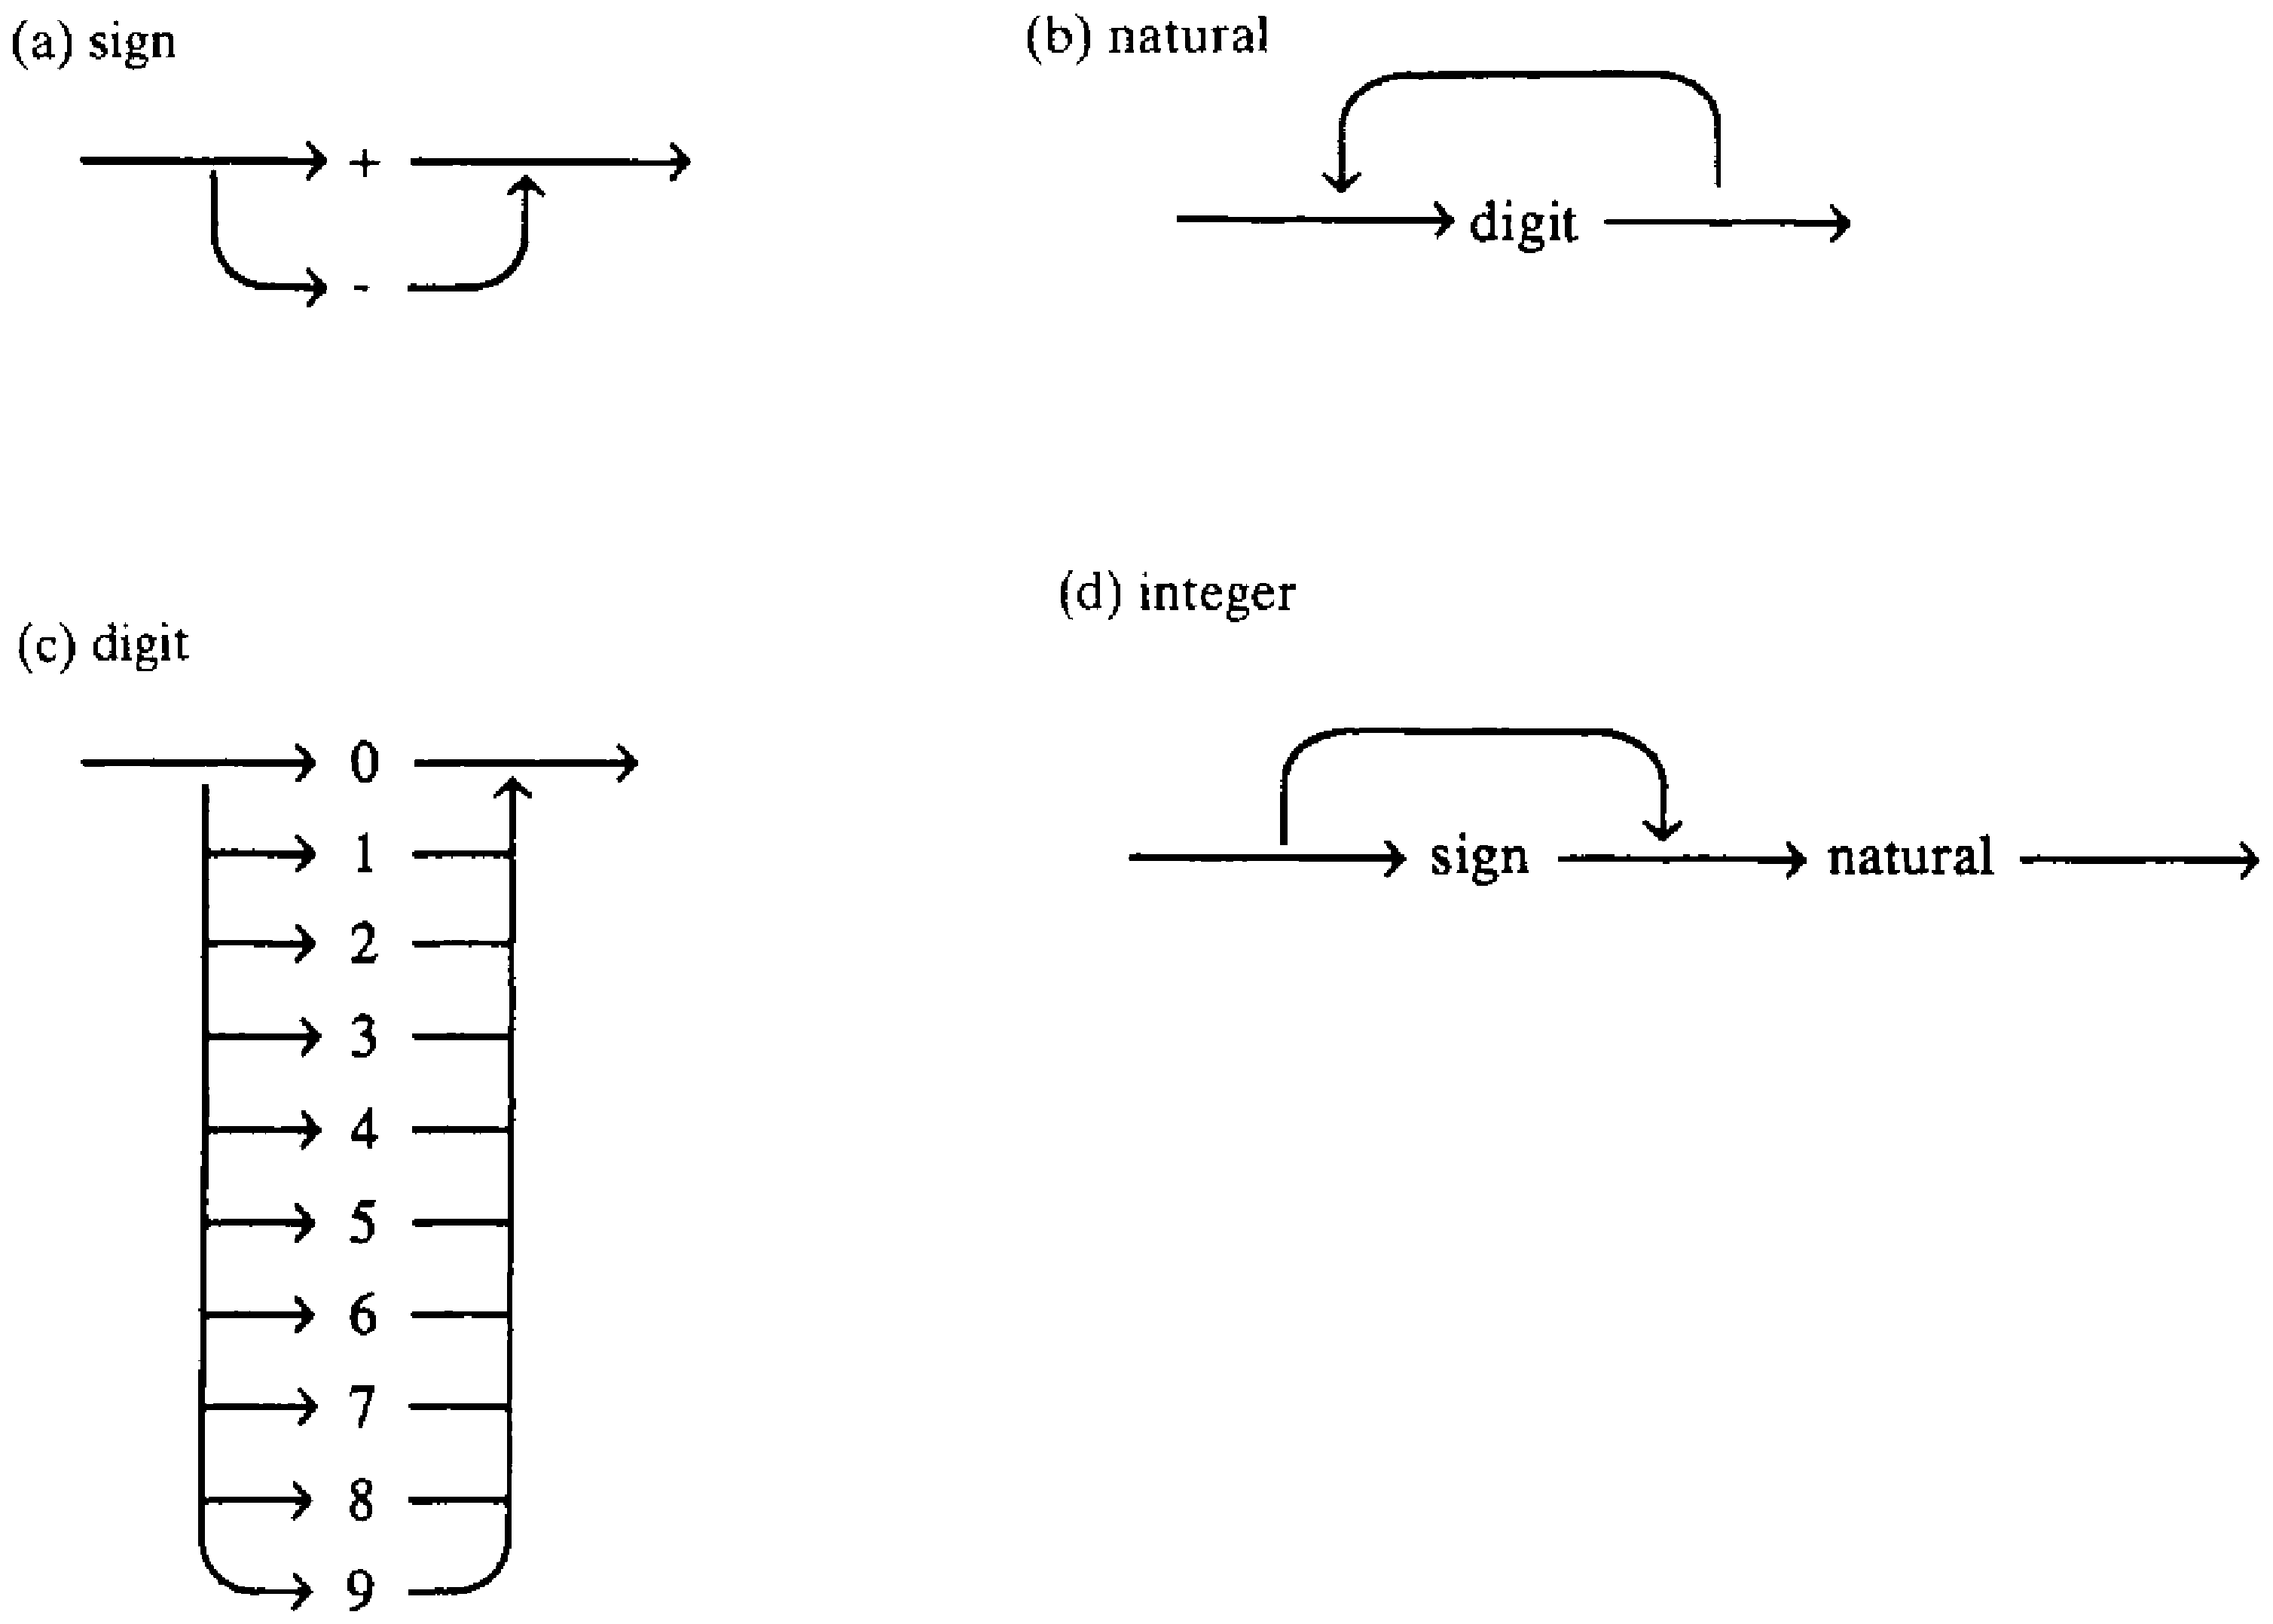
\epsfig{figure=ToFAfigures/fig0-6.eps,width=5.5in}}
%\centerline{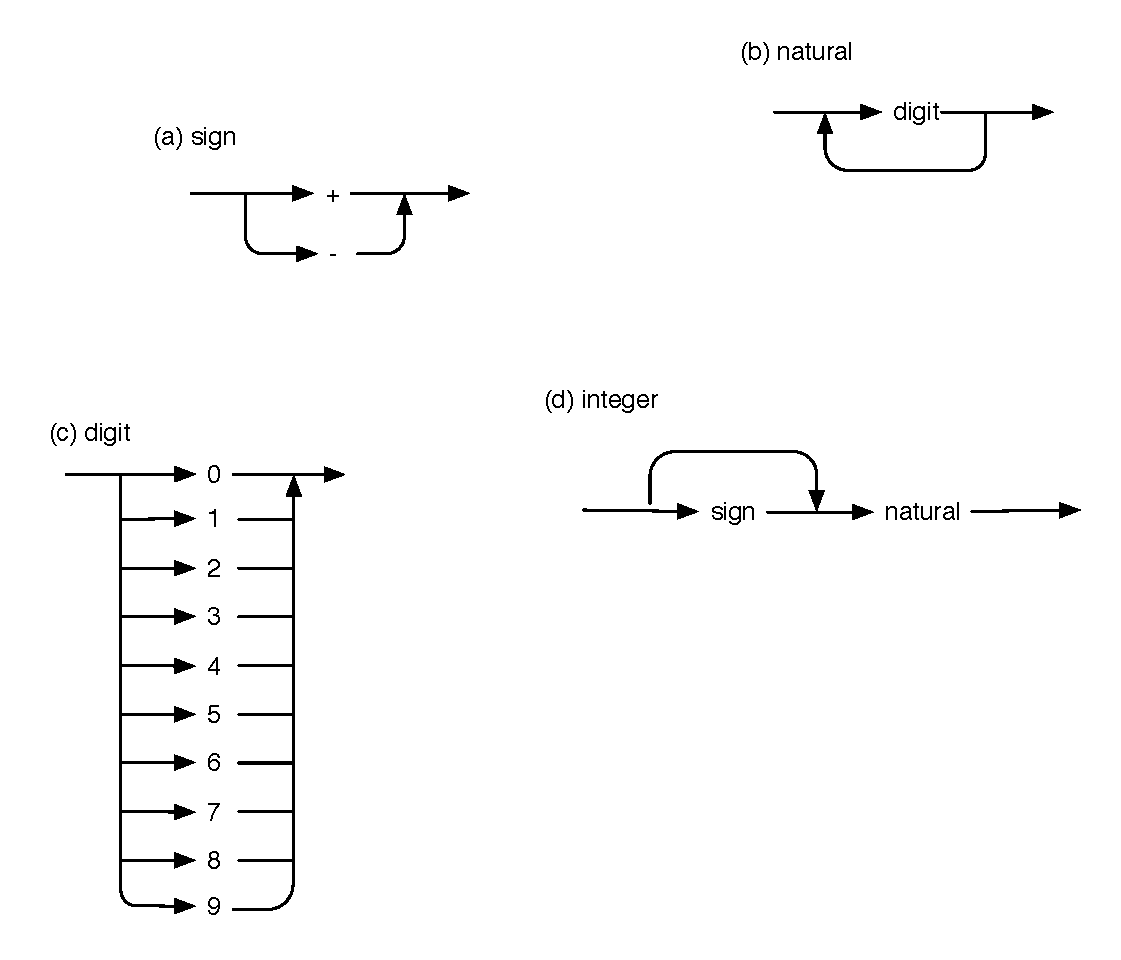
\epsfig{figure=Figures/fig-0-6.eps,width=\textwidth}}
%\centerline{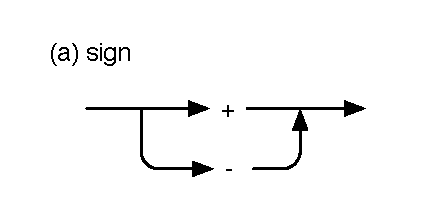
\epsfig{figure=Figures/fig-0-6-a.eps,width=0.25\textwidth}}
%\centerline{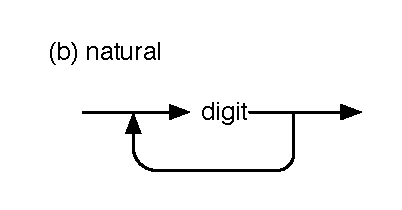
\epsfig{figure=Figures/fig-0-6-b.eps,width=0.25\textwidth}}
%\centerline{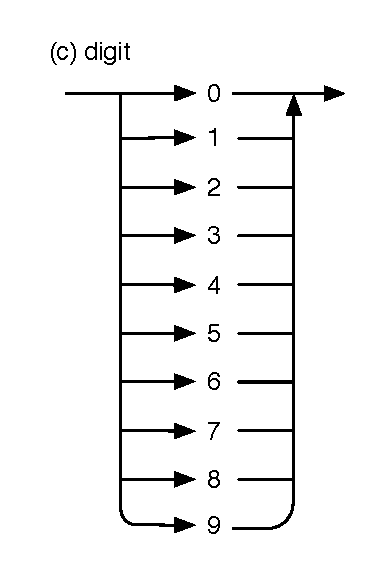
\epsfig{figure=Figures/fig-0-6-c.eps,width=0.25\textwidth}}
%\centerline{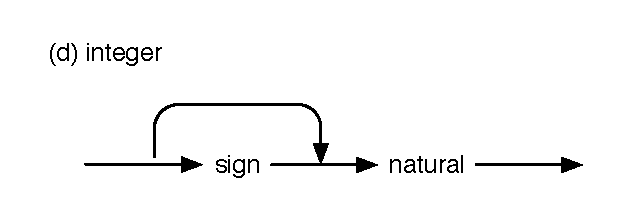
\epsfig{figure=Figures/fig-0-6-d.eps,width=0.25\textwidth}}
\caption{Syntax diagrams for the components of integer constants}\label{fig-0.6}
\end{figure}

\subsection*{Example 0.23}

The constraints for integer constants, which may begin with a sign and must
consist of one or more digits, are succinctly described by the following
\emph{productions} (replacement rules):
\begin{center}
\begin{tabular}{r@{ ::$=$ }l}
\<sign\> & $\pmb{+}|\pmb{-}$ \\
\<digit\> & $\pmb{0}|\pmb{1}|\pmb{2}|\pmb{3}|\pmb{4}|\pmb{5}|\pmb{6}|\pmb{7}|
	\pmb{8}|\pmb{9}$ \\
\<natural\> & \<digit\>$|$\<digit\>\<natural\>  \\
\<integer\> & \<natural\>$|$\<sign\>\<natural\> \\
\end{tabular}
\end{center}
The symbol $|$ represents ``or,'' and the rule
\[ \text{\<sign\> } ::= \pmb{+}|\pmb{-} \]
should be interpreted to mean that the token \<sign\> can be replaced by either
the symbol $\pmb{+}$ or the symbol $\pmb{-}$. A typical integer constant is
therefore $\pmb{+12}$, since it can be derived by applying the above rules in
the following fashion:
\begin{center}\begin{tabular}{r@{ $\rightarrow$ }l}
\<integer\> & \<sign\>\<natural\> \\
\<sign\>\<natural\> & $\pmb{+}$\<natural\> \\
$\pmb{+}$\<natural\> & $\pmb{+}$\<digit\>\<natural\> \\
$\pmb{+}$\<digit\>\<natural\> & $\pmb{+1}$\<natural\> \\
$\pmb{+1}$\<natural\> & $\pmb{+1}$\<digit\> \\
$\pmb{+1}$\<digit\> & $\pmb{+12}$
\end{tabular}\end{center}
Syntax diagrams for each of the four productions are shown in Figure \ref{fig-0.6}.
These can be combined to form a diagram that does not involve the intermediate
tokens \<sign\>, \<digit\>, and \<natural\> (see Figure \ref{fig-0.7}).

\begin{figure}[tb]
% Figure 0.7
%\centerline{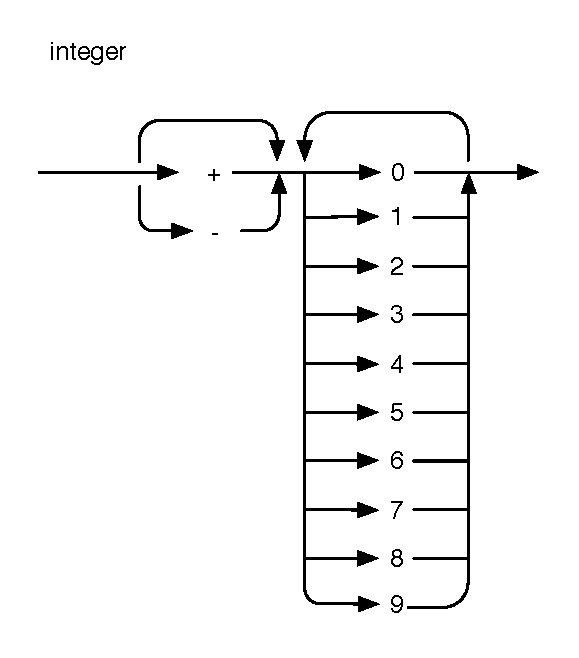
\epsfig{figure=Figures/fig-0-7.eps,width=\textwidth}}
\centerline{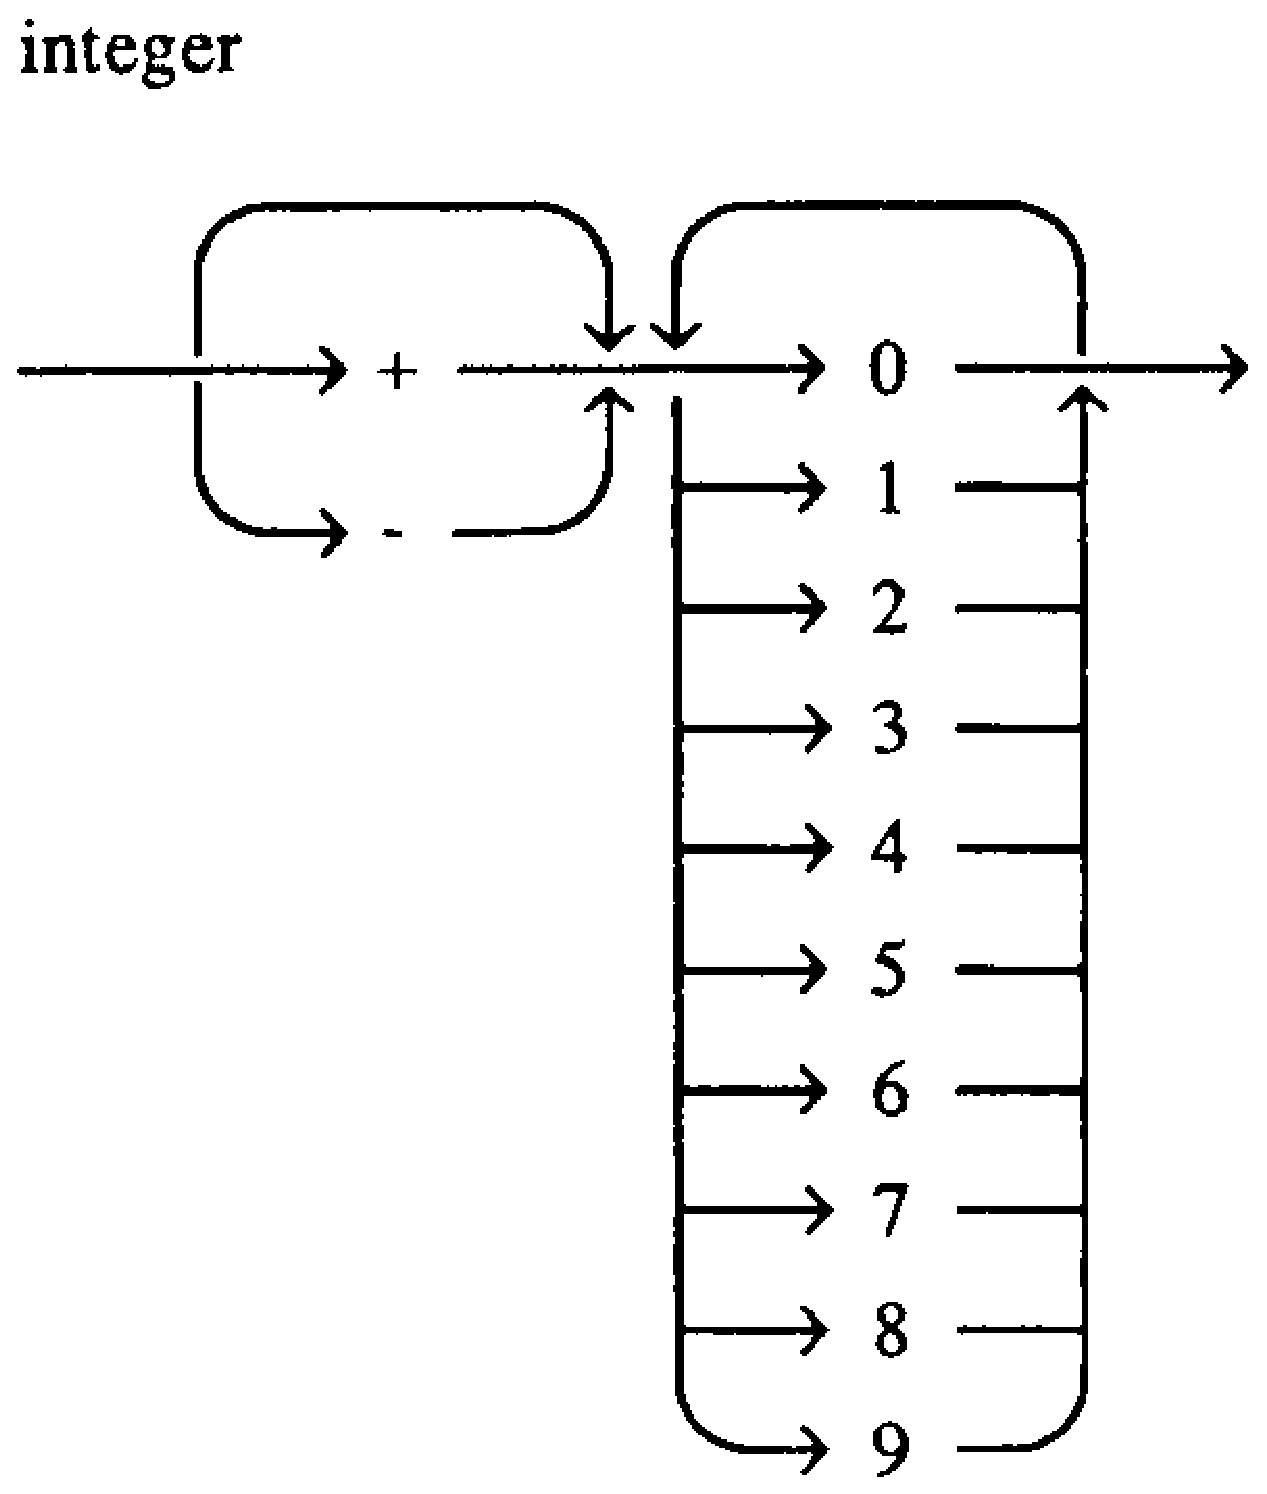
\epsfig{figure=ToFAfigures/fig0-7.eps,width=2.5in}}
\caption{A syntax diagram for integer constants}\label{fig-0.7}
\end{figure}

\section*{Exercises}\label{sec-0.exer}
\begin{enumerate}[{0.}1. ]
\item
Construct truth tables for:
\begin{enumerate}
\item
$\neg r \vee (\neg p \downarrow \neg q)$
\item
$(p \wedge \neg q) \vee \neg (p \uparrow  q)$
\end{enumerate}

\item
Draw circuit diagrams for:
\begin{enumerate}
\item $\neg (r \vee (\neg p \downarrow \neg q)) \uparrow (s \wedge p)$
\item $(p \wedge  \neg q) \vee \neg (p \uparrow q)$
\end{enumerate}

\item
Show that the sets $\{1, 2\} \times \{a, b\}$ 
and $\{a, b\} \times \{1, 2\}$ are not equal.

\item
Let $X =\{1, 2, 3, 4\}$.
\begin{enumerate}
\item
Determine the set of ordered pairs comprising the relation $<$.
\item
Determine the set of ordered pairs comprising the relation $=$.
\item
Since relations are sets of ordered pairs, it makes sense to union them
together.
Determine the set $= \cup <$.
\item
Determine the set of ordered pairs comprising the relation $\le$.
\end{enumerate}

\item
Let $n \in \NN$ be a natural number.
Show that congruence modulo $n$, $\equiv_n$, is an
equivalence relation.

\item
Let $X = \NN$.
Determine the equivalence classes for congruence modulo $0$.

\item
Let $X = \NN$. Determine the equivalence classes for congruence modulo $1$.

\item
Let $X = \RN$. Determine the equivalence classes for congruence modulo $1$.

\item
Let $R$ be an arbitrary equivalence relation in $X$.
Prove that the distinct equivalence classes of $R$ form a partition of $X$.

\item
Given a set $X$ and a partition $P = \{A_1,A_2, \ldots, A_n\}$ of $X$,
prove that $X$ equals the union of the sets in $P$.

\item
Given a set $X$ and a partition $P = \{A_1,A_2, \ldots, A_n\}$ of $X$, prove
that the relation $R(P)$ in $X$ induced by $P$ is an equivalence relation.

\item
Let $X = \{1, 2, 3, 4\}$.
\begin{enumerate}
\item
Give an example of a partition $P$ for which $R(P)$ is a function.
\item
Give an example of a partition $P$ for which $R(P)$ is not a function.
\end{enumerate}

\item
The following ``proof'' seems to indicate that a relation that is
symmetric and transitive must also be reflexive:

\begin{quote}
By symmetry, $x Ry \Rightarrow y Rx$. \\
Thus we have $(xRy \wedge yRx)$. \\
By transitivity, ($x Ry \wedge yRx) \Rightarrow x Rx$.\\
Hence $(\forall x)(x Rx)$.
\end{quote}

Find the flaw in this ``proof'' and give an example of a relation that is
symmetric and transitive but not reflexive.

\item
Let $R$ be an arbitrary equivalence relation in $X$. Prove that the equality
relation on $X$ refines $R$.

\item
Consider the ``function'' $t\!: \RN \rightarrow \RN$ defined by pairing $x$ with
the real number whose cosine is $x$.
\begin{enumerate}
\item
Show that $t$ is not well defined.
\item
Adjust the domain and range of $t$ to produce a valid function.
\end{enumerate}

\item
Consider the function $s'\!\!: \RN \rightarrow \RN$ defined by $s'(x) = x^2$ Show
that the converse of $s'$ is not a function.

\item
Let $\NNN$ be the set of nonnegative real numbers, and consider the function
$s$: $\NNN \rightarrow \NNN$ defined by $s(x)=x^2$. Show that $s^{-1}$ exists.

\item
Let $f$: $X\times Y$ be an arbitrary function. Prove that the converse of $f$ is
a function {\em iff} $f$ is a bijection.

\item
\begin{enumerate}
\item
Let $\sim$$A$ denote the complement of a set $A$. Prove that $\sim$$(\sim$$A) = A$.
\item
Let $\sim$$R$ denote the converse of a relation $R$. Prove that $\sim$$(\sim$$R) = R$
\end{enumerate}

\item
Let the functions $f$: $X \rightarrow Y$ and $g$: $Y \rightarrow Z$ be one to one.
Prove that $g \circ f$ is one to one.

\item
Let the functions $f$: $X \rightarrow Y$ and $g$: $Y \rightarrow Z$ be onto. Prove
that $g \circ f$ is onto.

\item
Define two functions for which $f\circ g = g\circ f$

\item
Define, if possible, a bijection between:
\begin{enumerate}
\item
$\NN$ and $\ZN$
\item
$\NN$ and $\NN \times \NN$
\item
$\NN$ and $\QN$
\item
$\NN$ and $\{a, b, c\}$
\end{enumerate}

\item
Use induction to prove that the sum of the cubes of the first $n$ positive
integers adds up to $\frac{n^2(n + 1)^2}{4}$

\item
Use induction to prove that the sum of the first $n$ positive integers is less
than $n^2$ (for $n > 1$).

\item
Use induction to prove that, for $n > 3$, $n! > n^2$.

\item
Use induction to prove that, for $n > 3, n! > 2^n$.

\item
Use induction to prove that $1^2 + 2^2 + \cdots + n^2 = n(n + 1)\frac{(2n + 1)}{6}$.

\item
Prove by induction that $X \cap (X_1 \cup X_2 \cup \cdots \cup X_n) =
(X \cap X_1) \cup (X \cap X_2) \cup \cdots \cup (X \cap X_n)$.

\item
Let $\sim A$ denote the complement of the set $A$. Prove by induction that
$\sim$$(X_1 \cup X_2 \cup \cdots \cup X_n) =
	(\sim$$X_1) \cap (\sim$$X_2) \cap \cdots \cap (\sim$$X_n)$.

\item
Use induction to prove that there are $2^n$ subsets of a set of size $n$; that
is, for any finite set $A$, $\|\wp(A)\| = 2^{\| A\|}$.

\item
The principle of mathematical induction is often stated in the following form,
which requires (apparently) stronger hypotheses to reach the desired conclusion:
Let $P(n)$ be a statement for each natural number $n \in \NN$. From the two
hypotheses
\begin{enumerate}[i.]
\item $P(0)$
\item $(\forall m \in \NN)(((\forall i \leq m)P(i)) \Rightarrow P(m + 1))$
\end{enumerate}
we can conclude $(\forall n \in \NN)P(n)$. Prove that the strong form of
induction is equivalent to the statement of induction given in the text.
\emph{Hint:} Consider the restatement of the hypothesis given in Example 0.22.

\item Determine what types of strings are defined by the following BNF:
\begin{center}\begin{tabular}{r@{ }l}
\<sign\> ::$=$ & $\pmb{+}|\pmb{-}$ \\
\<digit\> ::$=$ & $\pmb{0}|\pmb{1}|\pmb{2}|\pmb{3}|\pmb{4}|\pmb{5}|\pmb{6}|
	\pmb{7}|\pmb{8}|\pmb{9}$ \\
\<natural\> ::$=$ & \<digit\>$|$\<digit\>\<natural\> \\
\<integer\> ::$=$ & \<natural\>$|$\<sign\>\<natural\> \\
\<real constant\> ::$=$ & \<integer\> \\
& \<integer\>. \\
& \<integer\>.\<natural\> \\
& \<integer\>.\<natural\>{\bf E}\<integer\>
\end{tabular}\end{center}

\item A set $X$ is \emph{\Index{cofinite}} if the complement of $X$ (with respect to some generally
understood universal set) is finite. Let the universal set be $\ZN$. Give an
example of
\begin{enumerate}
\item A finite set
\item A cofinite set
\item A set that is neither finite nor cofinite
\end{enumerate}

\item Consider the equipotent relation, which relates sets to other sets.
\begin{enumerate}
\item Prove that this relation is reflexive.
\item Prove that this relation is symmetric.
\item Prove that this relation is transitive
\end{enumerate}

\item Define a function that will show that $\|\NN\| = \|\NN \times \NN\|$

\item Show that $\NN$ is equipotent to $\NN$.

\item Show that $\NN$ is equipotent to $\QN$.

\item Show that $\wp(\NN)$ is equipotent to $\{f$: $\NN\rightarrow\{$Yes, No$\}
\ |\ f$ is a function$\}$.

\item Show that $\wp(\NN)$ is equipotent to $\RN$.

\item Draw a circuit diagram that will implement the function $q$ given by the
truth table shown in Figure \ref{fig-0.8}.

\item \begin{enumerate}
\item Draw a circuit diagram that will implement the function $q_1$ given by the
truth table shown in Figure \ref{fig-0.9}.
\item Draw a circuit diagram that will implement the function $q_2$ given by the
truth table shown in Figure \ref{fig-0.9}.
\item Draw a circuit diagram that will implement the function $q_3$ given by the
truth table shown in Figure \ref{fig-0.9}.
\end{enumerate}
\end{enumerate}

% Figure 0.8
\begin{figure}[tb]
\begin{center}
\begin{tabular}{ccc|c}
$p_1$ & $p_2$ & $p_3$ & $q$\\
\hline
$\pmb{0}$ & $\pmb{0}$ & $\pmb{0}$ & $\pmb{0}$\\
$\pmb{0}$ & $\pmb{0}$ & $\pmb{1}$ & $\pmb{0}$\\
$\pmb{0}$ & $\pmb{1}$ & $\pmb{0}$ & $\pmb{1}$\\
$\pmb{0}$ & $\pmb{1}$ & $\pmb{1}$ & $\pmb{0}$\\
$\pmb{1}$ & $\pmb{0}$ & $\pmb{0}$ & $\pmb{1}$\\
$\pmb{1}$ & $\pmb{0}$ & $\pmb{1}$ & $\pmb{0}$\\
$\pmb{1}$ & $\pmb{1}$ & $\pmb{0}$ & $\pmb{0}$\\
$\pmb{1}$ & $\pmb{1}$ & $\pmb{1}$ & $\pmb{1}$
\end{tabular}
\end{center}
\caption{The truth table for Exercise 0.41}\label{fig-0.8}
\end{figure}

% Figure 0.9
\begin{figure}[tb]
\begin{center}
\begin{tabular}{cccc|ccc}
$p_1$ & $p_2$ & $p_3$ & $p_4$ & $q_1$ & $q_2$ & $q_3$\\
\hline
$\pmb{0}$ & $\pmb{0}$ & $\pmb{0}$ & $\pmb{0}$ & $\pmb{1}$ & $\pmb{1}$ & $\pmb{1}$\\
$\pmb{0}$ & $\pmb{0}$ & $\pmb{0}$ & $\pmb{1}$ & $\pmb{0}$ & $\pmb{1}$ & $\pmb{0}$\\
$\pmb{0}$ & $\pmb{0}$ & $\pmb{1}$ & $\pmb{0}$ & $\pmb{1}$ & $\pmb{0}$ & $\pmb{0}$\\
$\pmb{0}$ & $\pmb{0}$ & $\pmb{1}$ & $\pmb{1}$ & $\pmb{1}$ & $\pmb{1}$ & $\pmb{0}$\\
$\pmb{0}$ & $\pmb{1}$ & $\pmb{0}$ & $\pmb{0}$ & $\pmb{0}$ & $\pmb{1}$ & $\pmb{1}$\\
$\pmb{0}$ & $\pmb{1}$ & $\pmb{0}$ & $\pmb{1}$ & $\pmb{1}$ & $\pmb{0}$ & $\pmb{0}$\\
$\pmb{0}$ & $\pmb{1}$ & $\pmb{1}$ & $\pmb{0}$ & $\pmb{1}$ & $\pmb{1}$ & $\pmb{0}$\\
$\pmb{0}$ & $\pmb{1}$ & $\pmb{1}$ & $\pmb{1}$ & $\pmb{0}$ & $\pmb{0}$ & $\pmb{0}$\\
$\pmb{1}$ & $\pmb{0}$ & $\pmb{0}$ & $\pmb{0}$ & $\pmb{1}$ & $\pmb{0}$ & $\pmb{1}$\\
$\pmb{1}$ & $\pmb{0}$ & $\pmb{0}$ & $\pmb{1}$ & $\pmb{1}$ & $\pmb{0}$ & $\pmb{0}$\\
$\pmb{1}$ & $\pmb{0}$ & $\pmb{1}$ & $\pmb{0}$ & $\pmb{0}$ & $\pmb{1}$ & $\pmb{0}$\\
$\pmb{1}$ & $\pmb{0}$ & $\pmb{1}$ & $\pmb{1}$ & $\pmb{0}$ & $\pmb{0}$ & $\pmb{0}$\\
$\pmb{1}$ & $\pmb{1}$ & $\pmb{0}$ & $\pmb{0}$ & $\pmb{1}$ & $\pmb{1}$ & $\pmb{1}$\\
$\pmb{1}$ & $\pmb{1}$ & $\pmb{0}$ & $\pmb{1}$ & $\pmb{0}$ & $\pmb{1}$ & $\pmb{0}$\\
$\pmb{1}$ & $\pmb{1}$ & $\pmb{1}$ & $\pmb{0}$ & $\pmb{0}$ & $\pmb{1}$ & $\pmb{1}$\\
$\pmb{1}$ & $\pmb{1}$ & $\pmb{1}$ & $\pmb{1}$ & $\pmb{0}$ & $\pmb{0}$ & $\pmb{0}$
\end{tabular}
\end{center}
\caption{The truth table for Exercise 0.42}\label{fig-0.9}
\end{figure}

\chapter{Introduction and Basic Definitions}\label{ch-1}

This chapter introduces the concept of a \emph{\Index{finite automaton}}, which
is perhaps the simplest form of abstract computing device. Although finite
automata theory is concerned with relatively simple machines, it is an important
foundation of a large number of concrete and abstract applications. The
finite-state control of a finite automaton is also at the heart of more complex
computing devices such as \emph{finite-state transducers} (Chapter \ref{ch-7}),
\emph{pushdown automata} (Chapter \ref{ch-10}), and \emph{Turing machines}
(Chapter \ref{ch-11}).

Applications for finite automata can be found in the algorithms used for string
matching in text editors and spelling checkers and in the lexical analyzers used
by assemblers and compilers. In fact, the best known string matching algorithms
are based on finite automata. Although finite automata are generally thought of
as abstract computing devices, other non-computer applications are possible.
These applications include traffic signals and vending machines or any device in
which there are a finite set of inputs and a finite set of things that must be
``remembered'' by the device.

Briefly, a \emph{deterministic finite automaton}\index{deterministic finite automaton|see{DFA}}\index{DFA|see{finite automaton}}\index{automaton|see{DFA, NDFA, FST, MSM, PDA, DPDA,\linebreak LBA, Turing machine}}, also called a
\emph{\Index{recognizer}} or \emph{acceptor}\index{acceptor|see|{DFA}}, is a mathematical model of
a finite-state computing device that recognizes a set of \emph{words} over some
alphabet; this set of words is called the \emph{language} accepted by the
automaton. For each word over the alphabet of the automaton, there is a unique
path through the automaton; if the path ends in what is called a \emph{final} or
\emph{accepting} state, then the word traversing this path is in the language
\emph{accepted} by the automaton.

Finite automata represent one attempt at employing a finite description to
rigorously define a (possibly) infinite set of words (that is, a 
\emph{language}). Given such a description, the criterion for membership in the
language is straightforward and well-defined; there are simple algorithms for
ascertaining whether a given word belongs to the set. In this respect, such
devices model one of the behaviors we require of a compiler: recognizing
syntactically correct programs. Actually, finite automata have inherent
limitations that make them unsuitable for modeling the compilers of modern
programming languages, but they serve as an instructive first approximation.
Compilers must also be capable of producing object code from source code, and a
model of a simple translation device is presented in Chapter \ref{ch-7} and
enhanced in later chapters.

Logic circuitry can easily be devised to implement these automata in hardware.
With appropriate data structures, these devices can likewise be modeled with
software. An example is the highly interactive \Index{Turing's World}$^{\copyright}$, developed at
Stanford University by Jon Barwise and John Etchemendy. This
$\text{Apple}\textsuperscript{\textregistered}$ Macintosh graphics package and the accompanying
tutorial are particularly useful in experimenting with many forms of automata.
Both hardware and software approaches will be explored in this chapter. We begin
our formal treatment with some fundamental definitions.

\section{Alphabets and Words}\label{sec-1.1}

The devices we will consider are meant to react to and manipulate symbols.
Different applications may employ different character sets, and we will therefore
take care to explicitly mention the \emph{alphabet} under consideration.

% Definition 1.1
\begin{dfn}\label{dfn-1.1}
$\Sigma$ is an \emph{\Index{alphabet}} \ \ {\bf \emph{iff}} \ \ $\Sigma$ is a finite nonempty set of symbols.
\end{dfn}

An element of an alphabet is often called a letter, although there is no reason
to restrict symbols in an alphabet to consist solely of single characters. Some
familiar examples of alphabets are the 26-letter English alphabet and the \index{ASCII alphabet}ASCII
character set, which represents a standard set of computer codes. In this text
we will usually make use of shorter, simpler alphabets, like those given in
Example 1.1.

\subsection*{Example 1.1}
\begin{enumerate}[i.]
\item $\{0, 1\}$
\item $\{a,b,c\}$
\item $\{\langle 0, 0\rangle, \langle 0, 1\rangle, \langle 1, 0\rangle,
	\langle 1, 1\rangle \}$
\end{enumerate}

It is important to emphasize that the elements (letters) of an alphabet are not
restricted to single characters. In example (iii.) above, the alphabet is
composed of the ordered pairs in $\{0, 1\} \times \{0, 1\}$. Such an alphabet
will be utilized in Chapter \ref{ch-7} when we use sequential machines to
construct a simple binary adder.\index{binary alphabet}

Based on the definition of an alphabet, we can define composite entities called
\emph{words} or \emph{strings}, which are finite sequences of symbols from the
alphabet.

% Definition 1.2
\begin{dfn}\label{dfn-1.2}
For a given alphabet $\Sigma$ and a natural number $n$, a sequence of symbols
$\pmb{a}_1\pmb{a}_2\ldots\pmb{a}_n$ is a \emph{word} (or \emph{string}) {\em over
the alphabet $\Sigma$ of length $n$} iff for each $i=1,2,\ldots,n,\ \pmb{a}_i\in
\Sigma$.
\end{dfn}

As formally specified in Definition \ref{dfn-1.5}, the order in which the
symbols of the word occur will be deemed significant, and therefore a word of
length 3 can be identified with an ordered triple belonging to
$\Sigma \times \Sigma \times \Sigma$. Indeed, one may view the three-letter word
$\pmb{bca}$ as a convenient shorthand for the ordered triple $\langle \pmb{b, c, a}\rangle$.
A word over an alphabet is thus an ordered string of symbols, where each symbol
in the string is an element of the given alphabet. An obvious example of words
is what you are reading right now, which are words (or strings) over the
standard English alphabet. In some contexts, these strings of symbols are
occasionally called \emph{sentences}.

\subsection*{Example 1.2}

Let $\Sigma = \{\pmb{0},\pmb{1},\pmb{2},\pmb{3},\pmb{4},\pmb{5},\pmb{6},\pmb{7},
\pmb{8},\pmb{9}\}$; some examples of words over this alphabet are
\begin{enumerate}[i.]
\item $\pmb{42}$
\item $\pmb{242342}$
\end{enumerate}

Even though only three different members of $\Sigma$ occur in the second
example, the length of $\pmb{242342}$ is 6, as each symbol is counted each time
it occurs. To easily and succinctly express these concepts, the absolute value
notation will be employed to denote the length of a string. Thus, $|\pmb{42}|=2$,
$|\pmb{242342}|=6$, and $|\pmb{a}_1\pmb{a}_2\pmb{a}_3\pmb{a}_4|=4$.

% Definition 1.3
\begin{dfn}\label{dfn-1.3}
For a given alphabet $\Sigma$ and a word $x=\pmb{a}_1\pmb{a}_2\ldots\pmb{a}_n$
over $\Sigma$, $|x|$ denotes the length of $x$. That is, $|\pmb{a}_1\pmb{a}_2
\ldots\pmb{a}_n|=n$.
\end{dfn}

It is possible to join together two strings to form a composite word; this
process is called \emph{concatenation}. The concatenation of two strings of
symbols produces one longer string of symbols, which is made up of the
characters in the first string, followed immediately by the symbols of the
second string.

% Definition 1.4
\begin{dfn}\label{dfn-1.4}\index{concatenation!of strings}
Given an alphabet $\Sigma$, let $x = \pmb{a}_1,\ldots\pmb{a}_n$ and $y=\pmb{b}_1,
\ldots\pmb{b}_m$, be strings where each $\pmb{a}_i\in\Sigma$ and each $\pmb{b}_j
\in\Sigma$. The \emph{concatenation} of the strings $x$ and $y$, denoted by $x\cdot y$,
is the juxtaposition of $x$ and $y$; that is, $x\cdot y=\pmb{a}_1\ldots\pmb{a}_n
\pmb{b}_1\ldots\pmb{b}_m$.
\end{dfn}

Note in Definition \ref{dfn-1.4} that $|x \cdot y| = n + m = |x| + |y|$. Some
examples of string concatenation are
\begin{enumerate}[i.]
\item $\pmb{aaa}\cdot\pmb{bbb}=\pmb{aaabbb}$ 
\item {\bf home}$\cdot${\bf run} = {\bf homerun}
\item $\pmb{a}^2\cdot\pmb{b}^3=\pmb{aabbb}$
\end{enumerate}

Example (iii) illustrates a shorthand for denoting strings. Placing a
superscript after a symbol means that this entity is a string made by
concatenating it to itself the specified number of times. In a similar fashion,
$(\pmb{ac})^3$ is meant to express  $\pmb{acacac}$. Note that an \emph{equal}
sign was used in the above examples. Formally, two strings are equal if they
have the same number of symbols and these symbols match, character for character.

% Definition 1.5
\begin{dfn}\label{dfn-1.5}\index{equality!of strings}
Given an alphabet $\Sigma$, let $x=\pmb{a}_1\ldots\pmb{a}_n$ and $y=\pmb{b}_1
\ldots\pmb{b}_m$ be strings over $\Sigma$. $x$ and $y$ are equal iff $n = m$ and
for each $i=1,2,\ldots,n$, $\pmb{a}_i=\pmb{b}_i$.
\end{dfn}

The operation of concatenation has certain algebraic properties: it is
associative, and it is not commutative. That is,\index{associative law}\index{commutative law}
\begin{enumerate}[i.]
\item $(\forall x \in \Sigma^*)(\forall y \in \Sigma^*)(\forall z \in \Sigma^*)
	x \cdot (y \cdot z) = (x \cdot y ) \cdot z.$
\item For most strings $x$ and $y$, $x \cdot y \not= y \cdot x$. 
\end{enumerate}

When the operation of concatenation is clear from the context, we will adopt the 
convention of omitting the symbol for the operator (as is done in arithmetic
with the multiplication operator). Thus $xyz$ refers to $x \cdot y \cdot z$. In
fact, in Chapter \ref{ch-6} it will be seen that the operation of concatenation
has many algebraic properties that are similar to those of arithmetic
multiplication.

It is often necessary to count the number of occurrences of a given symbol
within a word. The notation described in the next definition will be an
especially useful shorthand in many contexts.

% Definition 1.6
\begin{dfn}\label{dfn-1.6}
Given an alphabet $\Sigma$, and some $\pmb{b} \in \Sigma$, the {\em length of a word
$w$ with respect to $\pmb{b}$}, denoted $|w|_{\pmb{b}}$, is the number of
occurrences of the letter $\pmb{b}$ within that word.
\end{dfn}

\subsection*{Example 1.3}
\begin{enumerate}[i.]
\item $|\pmb{abb}|_{\pmb{b}}=2$
\item $|\pmb{abb}|_{\pmb{c}}=0$
\item $|\pmb{1000000001118881888888}|_{\pmb{1}}=5$
\end{enumerate}

% Definition 1.7
\begin{dfn}\label{dfn-1.7}
Given an alphabet $\Sigma$, the \emph{\Index{empty word}}\index{empty string}, denoted by $\lambda$, is
defined to be the (unique) word consisting of zero letters.
\end{dfn}

The empty word is often denoted by $\epsilon$ in many formal language texts. The
empty string serves as the identity element for concatenation. That is, for all
strings $x$,
\[ x \cdot \lambda = \lambda \cdot x = x \]
Even though the empty word is represented by a single character,
$\lambda$ is a string but is \emph{not} a member of any alphabet:
$\lambda \notin \Sigma$.
(Symbols in an alphabet all have length one; $\lambda$ has length zero.)

A particular string $x$ can be divided into \emph{substrings} in several ways.
If we choose to break $x$ up into three substrings $u$, $v$, and $w$, there are
many ways to accomplish this. For example, if $x=\pmb{abccdbc}$, it could be
written as $\pmb{ab}\cdot\pmb{ccd}\cdot\pmb{bc}$; that is, $x=uvw$, where $u=
\pmb{ab}$, $v=\pmb{ccd}$, and $w=\pmb{bc}$. This $x$ could also be written as
$\pmb{abc}\cdot\lambda\cdot\pmb{cdbc}$, where $u=\pmb{abc}$, $v=\lambda$, and
$w=\pmb{cdbc}$. In this second case, $|x|=7=3+0+4=|u|+|v|+|w|$.

A fundamental structure in formal languages involves sets of words. A simple 
example of such a set is $\Sigma^k$, the collection of all words of exactly
length $k$ (for some $k \in \NN$) that can be constructed from the letters of 
$\Sigma$.

% Definition 1.8
\begin{dfn}\label{dfn-1.8}
Given an alphabet $\Sigma$ and a nonnegative integer $k \in \NN$, we define 
$$\Sigma^k = \{x \ | \ x\mbox{ is a word over $\Sigma$ and } |x| = k\}$$
\end{dfn}

\subsection*{Example 1.4} 

If 
\begin{align*}
\Sigma &= \{\pmb{0},\pmb{1}\}
\intertext{then}
\Sigma^0 &= \{\lambda\} \\
\Sigma^1 &= \{\pmb{0},\pmb{1}\} \\
\Sigma^2 &= \{\pmb{00},\pmb{01},\pmb{10},\pmb{11}\} \\
\Sigma^3 &= \{\pmb{000},\pmb{001},\pmb{010},\pmb{011},\pmb{100},\pmb{101},
	\pmb{110},\pmb{111}\}
\end{align*}
$\lambda$ is the only element of $\Sigma^0$, the set of all words containing
zero letters from $\Sigma$. There is no difficulty in letting $\lambda$ be an
element (and the only element) of $\Sigma^0$, since each $\Sigma^k$ is not
necessarily an alphabet, but is instead a set of words; $\lambda$, according to
the definition, is indeed a word consisting of zero letters.

% Definition 1.9
\begin{dfn}\label{dfn-1.9}
Given an alphabet $\Sigma$, define
\[\Sigma^* = \bigcup\limits^\infty_{k=0} \Sigma^k = \Sigma^0 \cup \Sigma^1 \cup
	\Sigma^2 \cup \Sigma^3 \cup \ldots \]
and
\[ \Sigma^+ = \bigcup\limits^\infty_{k=1} \Sigma^k = \Sigma^1 \cup \Sigma^2 \cup
	\Sigma^3 \cup \ldots \]
\end{dfn}
$\Sigma^*$ is the set of all words that may be constructed from the
letters of an alphabet $\Sigma$. $\Sigma^+$ is the set of all \emph{nonempty}
words that may be constructed from $\Sigma$.

$\Sigma^*$, like the set of natural numbers, is an infinite set. Although
$\Sigma^*$ is infinite, each word in $\Sigma^*$ is of finite length. This
property follows from the definition of $\Sigma^*$ and a property of natural
numbers: any $k \in \NN$ must by definition be a finite number. $\Sigma^*$ is
defined to be the union of all $\Sigma^k,\ k \in \NN$. Since each such $k$ is a
finite number and every word in $\Sigma^k$ is of length $k$, then every word in
$\Sigma^k$ must be of finite length. Furthermore, since $\Sigma^*$ is the union
of all such $\Sigma^k$, every word in $\Sigma^*$ must also be of finite length.
While $\Sigma^*$ can contain arbitrarily long words, each of these words must
be finite, just as every number in $\NN$ is finite.

Since $\Sigma^*$ is the union of all $\Sigma^k$ for $k \in \NN,\ \Sigma^*$ must
also contain $\Sigma^0$. In other words, besides containing all words that can
be constructed from one or more letters of $\Sigma$, $\Sigma^*$ also contains
the empty word $\lambda$. While $\lambda \notin \Sigma,\ \lambda \in \Sigma^*$.
$\lambda$ represents a \emph{string} and \emph{not} a symbol, and thus the empty
string cannot be in the alphabet $\Sigma$. However, $\lambda$ is included in
$\Sigma^*$, since $\Sigma^*$ is not just an alphabet, but a collection of words
over the alphabet $\Sigma$. Note, however, that $\Sigma^+$ is
$\Sigma^* - \{\lambda\};\ \Sigma^+$ specifically excludes $\lambda$.

\section{Definition of a Finite Automaton}\label{sec-1.2}

We now have the building blocks necessary to define deterministic finite
automata. A \emph{deterministic finite automaton} is a mathematical model of a
machine that accepts a particular set of words over some alphabet $\Sigma$.

A useful visualization of this concept might be referred to as the
\index{black box model}\emph{black box} model. This conceptualization is built around a black box that
houses the \emph{finite-state control}. This control reacts to the information
provided by the \emph{read head}, which extracts data from the \emph{input tape}.\index{tape!input}
The control also governs the operation of the output indicator, often depicted
as an \emph{acceptance light}, as shown in Figure \ref{fig-1.1}.

There is no limit to the number of symbols that can be on the tape (although
each individual word must be of finite length). As the input tape is read by the
machine, \emph{state transitions}, which alter the current \emph{state} of the
automaton, take place within the black box. Depending on the word contained on
the input tape, the light bulb either lights or remains dark when the end of the
input string is reached, indicating acceptance or rejection of the word,
respectively. We assume that the input head can sense when it has passed the
last symbol on the tape. In some sense, a personal computer fits the
finite-state control model; it reacts to each keystroke entered from the
keyboard according to the current state of the CPU and its own internal memory.
However, the number of possible bit patterns that even a small computer can
assume is so astronomically large that it is totally impractical to model a
computer in this fashion. Finite-state machines can be profitably used to
describe portions of a computer (such as parts of the arithmetic/logic unit, as
discussed in Chapter \ref{ch-7}, Example 7.15) and other devices that
assume a reasonable number of states.

% Figure 1.1
\begin{figure}
%\centerline{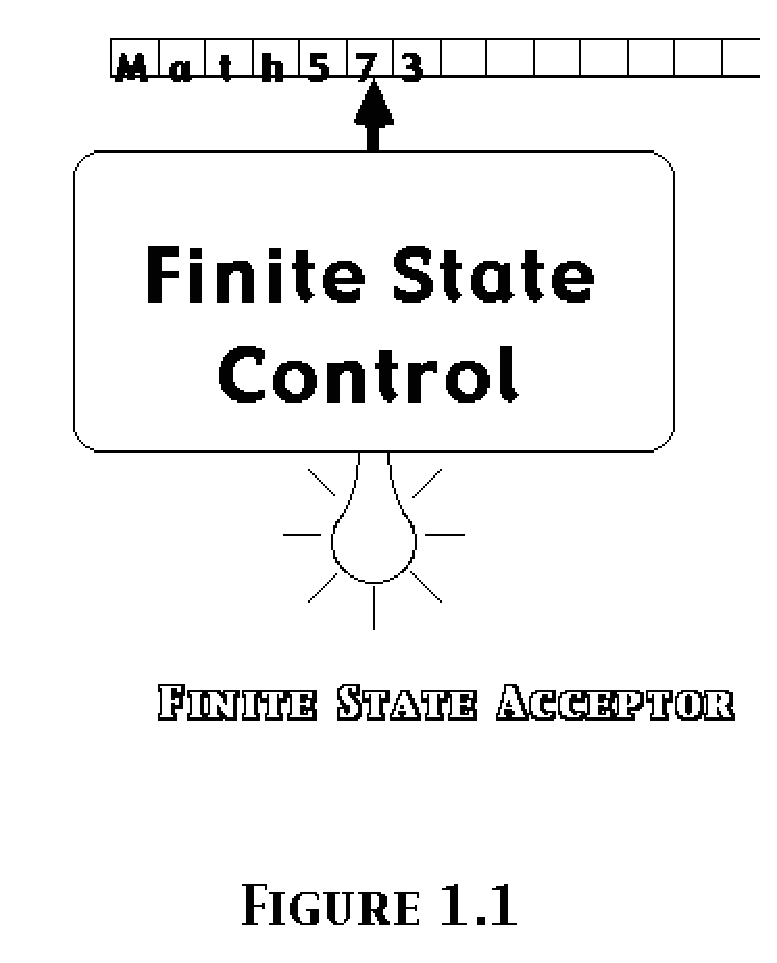
\epsfig{figure=Figures/fig-1-1.eps,height=2in}}
\centerline{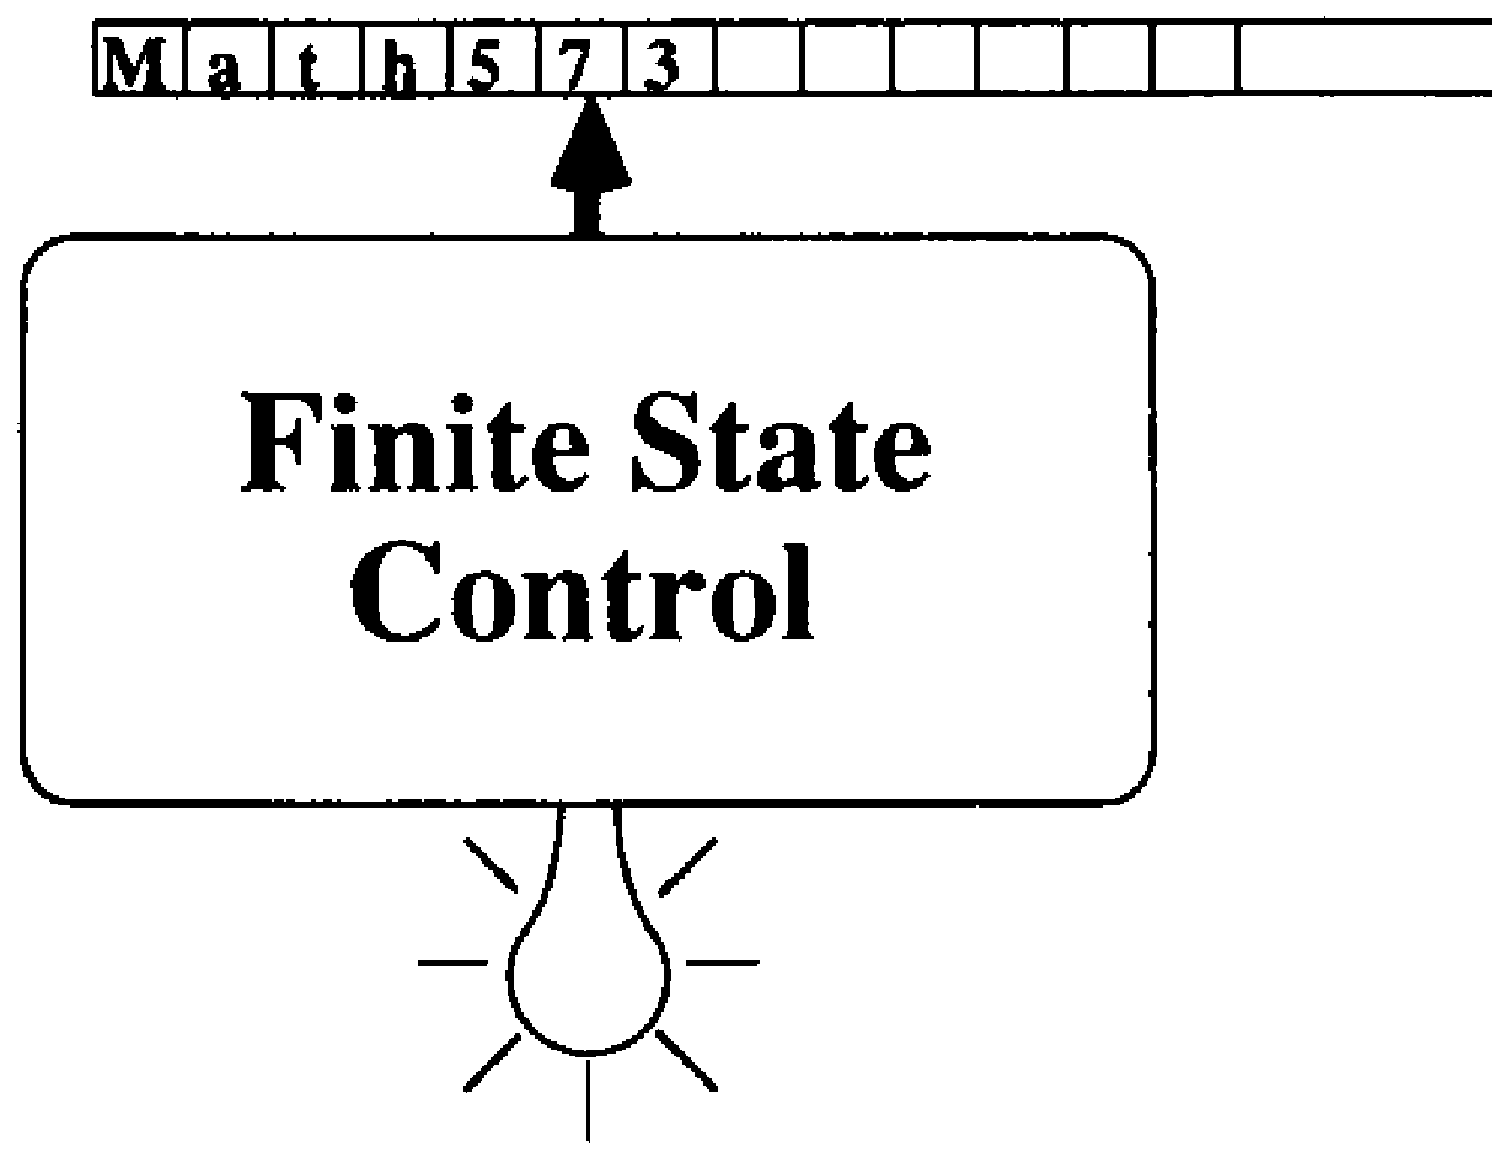
\epsfig{figure=ToFAfigures/fig1-1.eps,height=2in}}
\caption{A model of a finite-state acceptor (DFA)}\label{fig-1.1}
\end{figure}

Although finite automata are usually thought of as processing strings of letters
over some alphabet, the input can conceptually be elements from any finite set.
A useful example is the ``brain'' of a vending machine, which, say, dispenses
30\cent\ candy bars.

\subsection*{Example 1.5}

The input to the vending machine is the set of coins \{nickel, dime, quarter\},
represented by $\pmb{n}$, $\pmb{d}$, and $\pmb{q}$ in Figure \ref{fig-1.2}. The
machine may only ``remember'' a finite  number of things; in this case, it will
keep track of the amount of money that has been dropped into the machine. Thus,
the machine may be in the ``state'' of remembering that no money has yet been
deposited (denoted in this example by \<0\cent\>), or that a single nickel has
been inserted (the state labeled \<5\cent\>, or that either a dime or two
nickels have been deposited \<10\cent\>, and so on. Note that from state
\<0\cent\> there is an arrow labeled by the dime token $\pmb{d}$ pointing to the
state \<10\cent\>, indicating that, at a time when the machine ``believes'' that
no money has been deposited, the insertion of a dime causes the machine to
transfer to the state that remembers that ten cents has been deposited. From the
\<0\cent\> state, the arrows in the diagram show that if two nickels ($\pmb{n}$)
are input the machine moves through the \<5\cent\> state and likewise ends in
the state labeled \<10\cent\>.

The vending machine thus counts the amount of change dropped into the machine
(up to 50\cent). The machine begins in the state labeled \<0\cent\> and follows
the arrows to higher-numbered states as coins are inserted. For example,
depositing a nickel, a dime, and then a quarter would move the machine to the
states \<5\cent\>, \<15\cent\>, and then \<40\cent\>. The states labeled
30\cent\ and above are doubly encircled to indicate that enough money has been
deposited; if 30\cent\ or more has been deposited, then the machine ``accepts,''
indicating that a candy bar may be selected.\index{vending machine!DFA}

% Figure 1.2
\begin{figure}
%\centerline{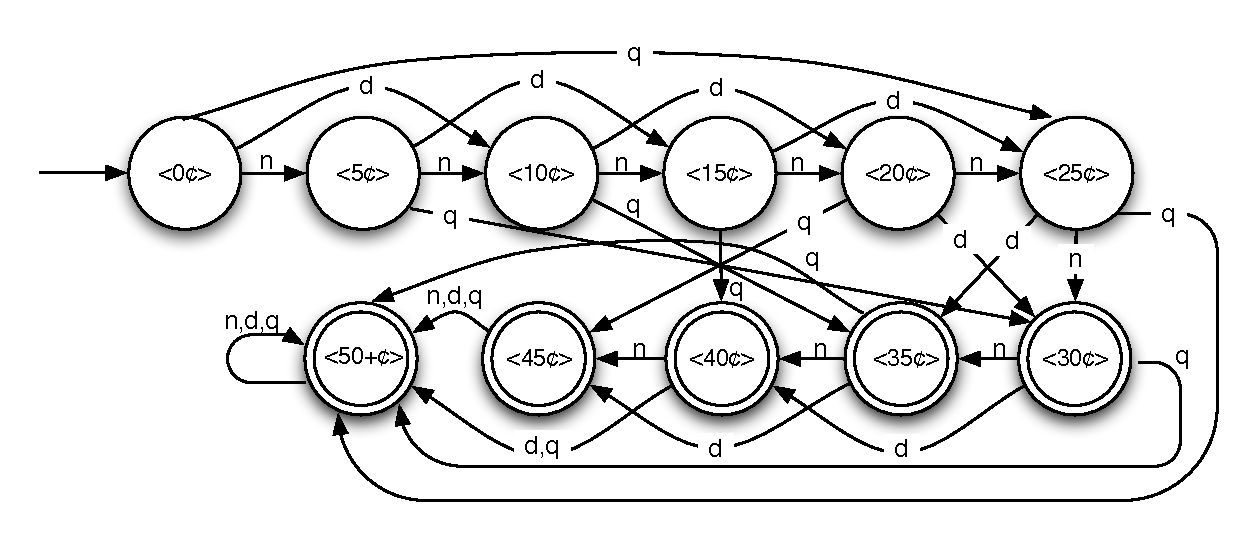
\epsfig{figure=Figures/fig-1-2.eps,width=\textwidth}}
\centerline{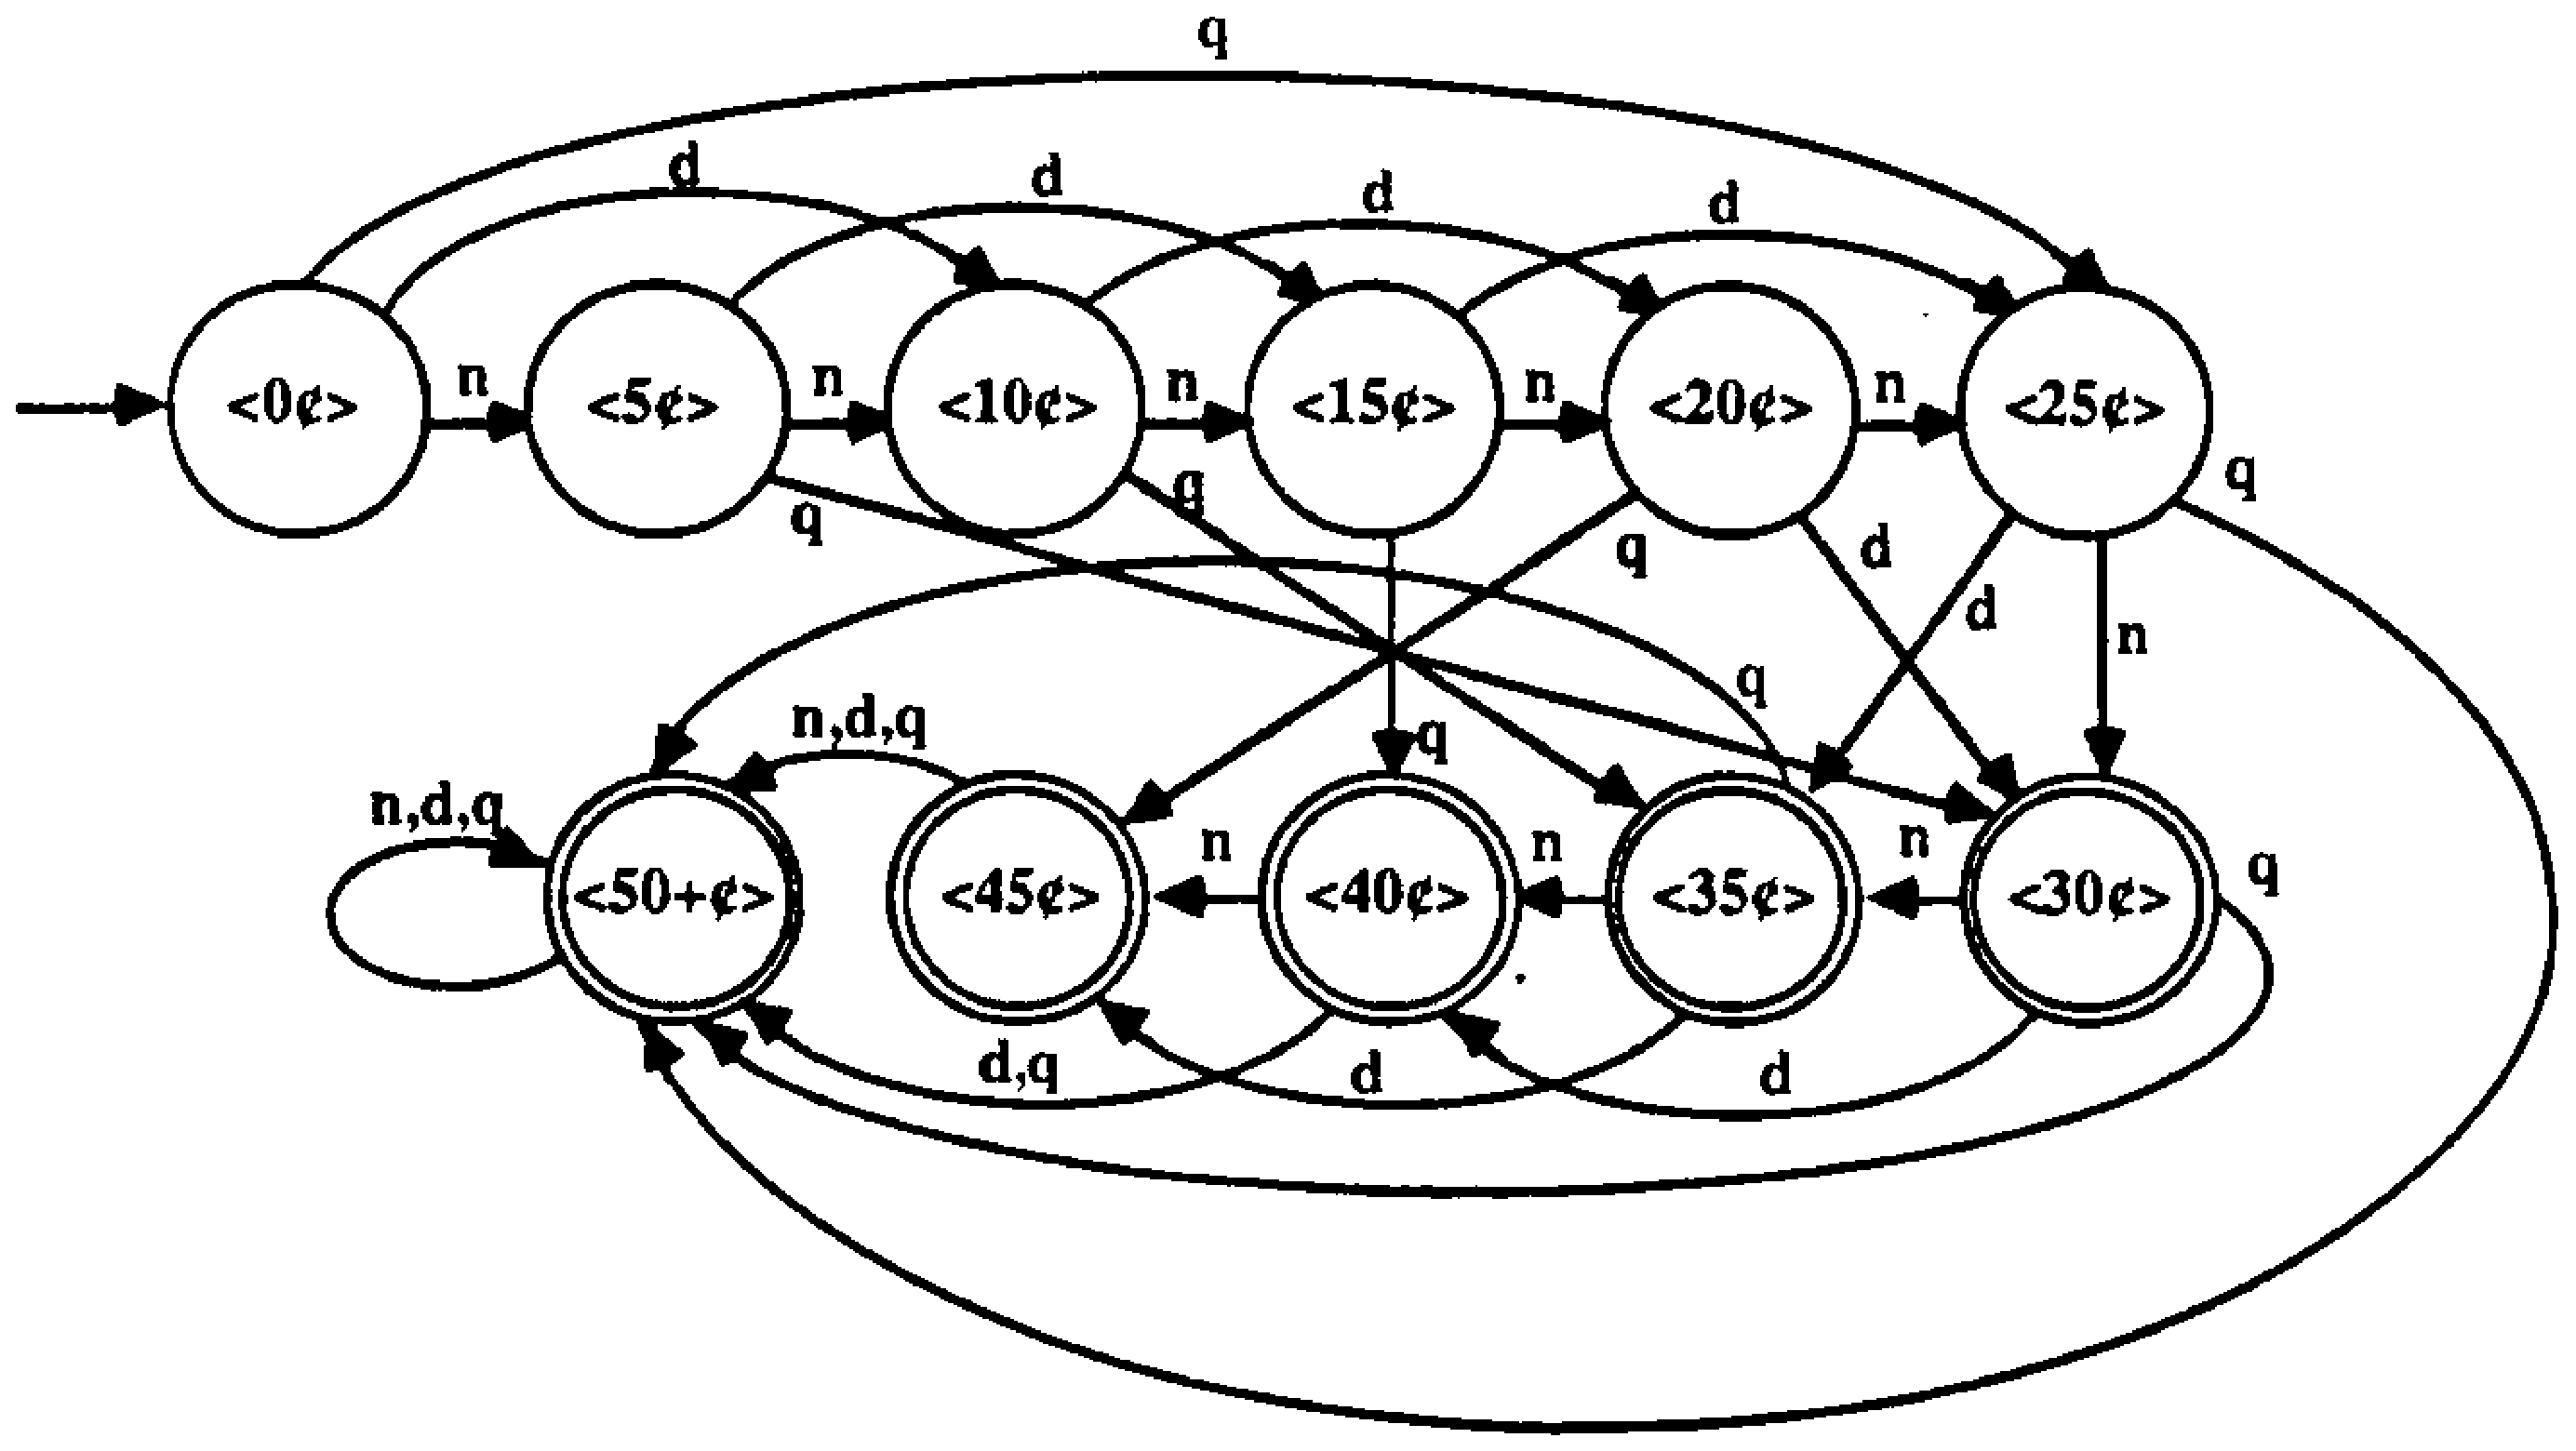
\epsfig{figure=ToFAfigures/fig1-2.eps,width=5in}}
\caption{An implementation of a vending machine}\label{fig-1.2}
\end{figure}

Finite automata are appropriate whenever there are a finite number of inputs and
only a finite number of situations must be distinguished by the machine. Other
applications include traffic signals and elevators (as discussed in Chapter
\ref{ch-7}). We now present a formal mathematical definition of a finite-state
machine.

% Definition 1.10
\begin{dfn}\label{dfn-1.10}\index{deterministic finite acceptor|see{DFA}}\index{final state!for DFA}\index{accepting state (DFA)}\index{alphabet!input}\index{D@ $\delta$ function|see{state transition function} }\index{state transition function!for DFA}

A \emph{deterministic finite automaton} or \emph{deterministic
finite acceptor} (\Index{DFA}) is a quintuple
\\$\langle\Sigma,S,s_0,\delta,F
\rangle$, where
\begin{enumerate}[i.]
\item $\Sigma$ is the \emph{input alphabet} (a finite nonempty set of symbols).
\item $S$ is a finite nonempty set of \emph{states}.
\item $s_0$ is the \emph{start} (or \emph{initial}) state,\index{start state}\index{initial state|see{start state}} an element of $S$.
\item $\delta$ is the \emph{state transition function};
	$\delta$: $S \times \Sigma \rightarrow S$.
\item $F$ is the set of \emph{final} (or \emph{accepting}) states, a (possibly
	empty) subset of $S$.
\end{enumerate}
\end{dfn}

The input alphabet, $\Sigma$, for any deterministic finite automaton A, is the
set of symbols that can appear on the input tape. Each successive symbol in a
word will cause a transition from the present state to another state in the
machine. As specified by the $\delta$ function, there is exactly one such state
transition for each combination of a symbol $a \in \Sigma$ and a state $s \in S$.
This is the origin of the word ``deterministic'' in the phrase ``deterministic
finite automaton.''\index{finite automaton!deterministic}

The various states represent the memory of the machine. Since the number of
states in the machine is finite, the number of distinguishable situations that
can be remembered by the machine is also finite. This limitation of the device's
ability to store its past history is the origin of the word ``finite'' in the
phrase ``deterministic finite automaton.'' At any given time during processing,
if the previous history of the machine is considered to be the reactions of the
DFA to the letters that have already been read, then the current state
represents all that is known about the history of the machine.

The start state of the machine is the state in which the machine always begins
processing a string. From this state, successive input symbols from $\Sigma$ are
used by the $\delta$ function to arrive at successive states in the machine.
Processing stops when the string of symbols is exhausted. The state in which the
machine is left can either be a final state, in which case the word is
\emph{accepted}, or it can be any one of the other states of $S$, in which case
the word is \emph{rejected}.\index{accept by final state}

To produce a formal description of the concepts defined above, it is necessary
to enumerate each part of the quintuple that comprises the DFA. $\Sigma$, $S$,
$s_0$, and $F$ are easily enumerated, but the function $\delta$ can often be
tedious to describe. One device used to display the mapping $\delta$ is the
\emph{state transition diagram}. Besides graphically displaying the transitions
of the $\delta$ function, the state transition diagram for a deterministic
finite automaton also illustrates the other four parts of the quintuple.

A finite automaton state transition diagram is a directed graph. The states of
the machine represent the vertices of the graph, while the mapping of the
$\delta$ function describes the edges. Final states are denoted by a doubly
encircled state, and the start state is identified by a straight incoming arrow.
Each domain element of the transition function corresponds to an edge in the
directed graph. We formally define a finite automaton state transition diagram
for $\langle\Sigma,S,s_0,\delta,F\rangle$ as a directed graph $G=\langle V,E
\rangle$, as follows:
\begin{enumerate}[i.]
\item $V=S$,
\item $E=\{\langle s,t,\pmb{a}\rangle | s,t\in S,\pmb{a}\in\Sigma\wedge\delta
	(s,\pmb{a})=t\}$,
\end{enumerate}
where $V$ is the set of vertices of the graph, and $E$ is the set of edges
connecting these vertices. Each element of $E$ is an ordered triple,
$\langle s,t,\pmb{a}\rangle$, such that $s$ is the origin vertex, $t$ is the
terminus, and $\pmb{a}$ is the letter from $\Sigma$ labeling the edge. Thus, for
any vertex there is exactly one edge leaving that vertex for each element of
$\Sigma$.

% Figure 1.3
\begin{figure}
%\centerline{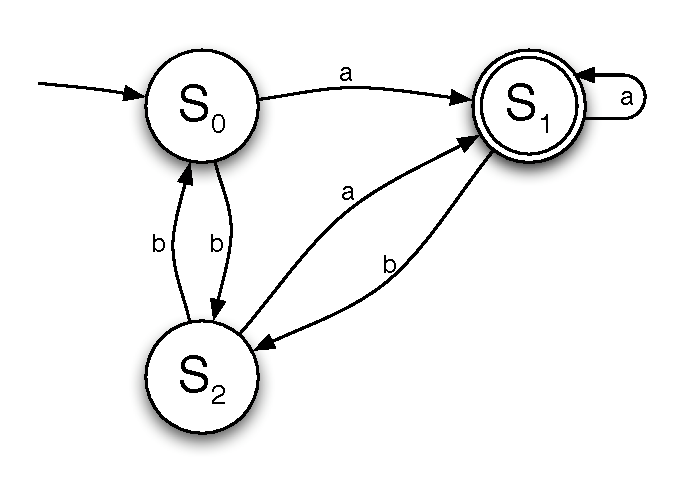
\epsfig{figure=Figures/fig-1-3.eps,width=\textwidth}}
\centerline{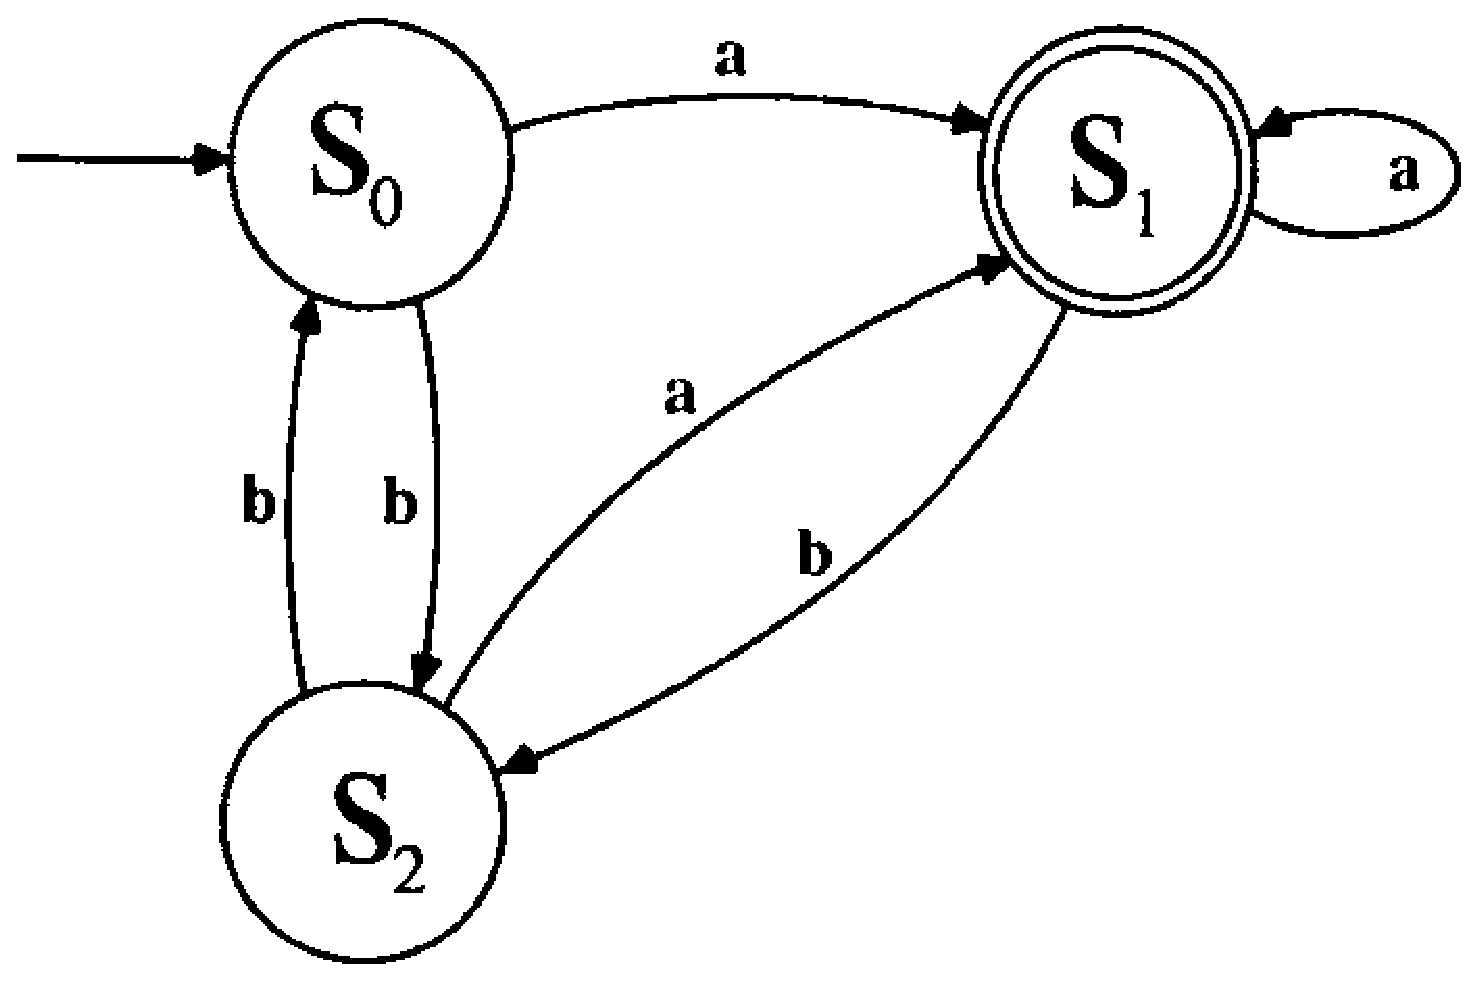
\epsfig{figure=ToFAfigures/fig1-3.eps,width=3in}}
\caption{The DFA described in Example 1.6}\label{fig-1.3}
\end{figure}

% Figure 1.4
\begin{center}
\begin{figure}
\begin{verbatim}
type
   Sigma = 'a'..'c';
   State = (s0,s1,s2);
var
   TransitionTable=array[State,Sigma] of State;

function Delta(S:State;A:Sigma):State;
begin
   Delta := TransitionTable [S, A]
end; {Delta}
\end{verbatim}
\caption{A Pascal implementation of a state transition function}\label{fig-1.4}
\end{figure}
\end{center}

\subsection*{Example 1.6}

In the DFA shown in Figure \ref{fig-1.3}, the set of edges $E$ of the graph $G$
is given by $E = \{\langle s_0,s_1,\pmb{a}\rangle,\langle s_0,s_2,\pmb{b}\rangle, \\
\langle s_1,s_1,\pmb{a}\rangle, \langle s_1,s_2,\pmb{b}\rangle, \langle s_2,s_1,
\pmb{a}\rangle,\langle s_2,s_0,\pmb{b}\rangle\}$. The figure also shows that
$s_0$ is the designated start state and that $s_1$ is the only final state. The
state transition function for a finite automaton is often represented in the
form of a \emph{state transition table}. A state transition table is a matrix
with the rows of the matrix labeled and indexed by the states of the machine,
and the columns of the matrix labeled and indexed by the elements of the input
alphabet; the entries in the table are the states to which the DFA will move.
Formally, let $T$ be a state transition table for some deterministic finite
automaton $A =\langle\Sigma,S,s_0,\delta,F\rangle$, and let $s \in S$ and
$\pmb{a}\in\Sigma$. Then the value of each matrix entry is given by the equation
\[ (\forall s\in S)(\forall\pmb{a}\in\Sigma)T_{s\pmb{a}}=\delta(s,\pmb{a}) \]
For the automaton in Example 1.6, the state transition table is
\begin{center}\begin{tabular}{c|cc}
$\delta$ & $\pmb{a}$ & $\pmb{b}$\\
\hline
$s_0$ & $s_1$ & $s_2$\\
$s_1$ & $s_1$ & $s_2$\\
$s_2$ & $s_1$ & $s_0$
\end{tabular}\end{center}
This table represents the following transitions:
\begin{align*}
&\delta(s_0,\pmb{a}) = s_1 &\delta(s_0,\pmb{b}) = s_2 \\
&\delta(s_1,\pmb{a}) = s_1 &\delta(s_1,\pmb{b}) = s_2 \\
&\delta(s_2,\pmb{a}) = s_1 &\delta(s_2,\pmb{b}) = s_0
\end{align*}

State transition tables are the most common method of representing the basic
structure of an automaton within a computer. When represented as an array in the
memory of the computer, access is very fast and the structure lends itself
easily to manipulation by the computer. Techniques such as depth-first search
are easily and efficiently implemented when the state transition diagram is
represented as a table. Figure \ref{fig-1.4} illustrates an implementation of
the $\delta$ function via transition tables in Pascal.

With $\delta$, we can describe the state in which we will find ourselves after
processing a single letter. We also want to be able to describe the state at
which we will arrive after processing an entire string. We will extend the
$\delta$ function to cover entire \emph{strings} rather than just single 
\emph{letters}; $\DBAR(s,x)$ will be the state we wind up at when
starting at $s$ and processing, in order, all the letters of the string $x$.
While this is a relatively easy concept to (vaguely) state in English, it is
somewhat awkward to formally define. To facilitate formal proofs concerning
DFAs, we use the following recursive definition.

% Definition 1.11
\begin{dfn}\label{dfn-1.11}\index{extended state transition function \DBAR\! for DFA}
\index{D@ $\overline \delta$|see{extended state transition function \DBAR}}
Given a DFA $A=\langle\Sigma,S,s_0,\delta,F\rangle$, the \emph{extended
state transition function for $A$}, denoted $\DBAR$, is a function $\DBAR$:
$S\times\Sigma^*\rightarrow S$ defined recursively as follows:
\\ \\
\begin{tabular}{r@{ }l@{$\qquad$}l@{ $=$ }l}
i. & $(\forall s\in S)(\forall\pmb{a}\in\Sigma)$ & $\DBAR(s,\pmb{a})$ &
	$\delta(s,\pmb{a})$ \\
ii. & $(\forall s\in S)$ & $\DBAR(s,\lambda)$ & $s$ \\
iii. & $(\forall s\in S)(\forall x\in\Sigma^*)(\forall\pmb{a}\in\Sigma)$ &
	$\DBAR(s,\pmb{a}x)$ & $\DBAR(\delta(s,\pmb{a}),x)$
\end{tabular}
\end{dfn}

The $\DBAR$ function extends the $\delta$ function from single
letters to words. Whereas the $\delta$ function maps pairs of states and
\emph{letters} to other states, the $\DBAR$ function maps pairs of
states and \emph{words} to other states. (i.) is the observation that $\delta$
and $\DBAR$ treat single letters the same; this fact is not really
essential to the definition of $\DBAR$, since it can be deduced from
(ii.) and (iii.) (see the exercises).

The $\DBAR$ function maps the current state $s$ and the first letter
$\pmb{a}_1$, of a word $w=\pmb{a}_1\ldots\pmb{a}_n$ via the $\delta$ function to
some other state $t$. It is then recursively applied with the new state $t$ and
the remainder of the word, that is, with $\pmb{a}_2\ldots\pmb{a}_n$. The
recursion stops when the remainder of the word is the empty word $\lambda$. See
Examples 1.7 and 1.11 for illustrations of computations using
this recursive definition.

Since the recursion of the $\DBAR$ function all takes place at the
end of the string, $\DBAR$ is called \emph{tail recursive}. \Index{Tail recursion}
is easily transformed into iteration by applying the $\delta$ to successive
letters of the input word and using the result of the previous application of
$\DBAR$ as an input to the current application.

Figure \ref{fig-1.5} gives an implementation of the $\DBAR$ function in
Pascal. Recursion has been replaced by iteration, and previous function results
are saved in an auxiliary variable T. The function Delta, the input alphabet
Sigma, and the state set State agree with the definitions given in Figure
\ref{fig-1.4}.

It stands to reason that if we start in state $s$ and word $y$ takes us to state
$r$, and if we start in state $r$ and word $x$ takes us to state $t$, then the
word $yx$ should take us from state $s$ all the way to $t$. That is, if
$\DBAR(s,y) = r$ and $\DBAR(r,x) = t$, then
$\DBAR(s,yx)$ should equal $t$, also. We can indeed prove this, as
shown with the following theorem.

% Theorem 1.1
\begin{thm}\label{thm-1.1}
Let $A =\langle\Sigma,S,s_0,\delta,F\rangle$ be a DFA. Then

\ \ \ \ \ \ \ \ \ \ \ \ \ \ \ \ \ \ \ \ 
$(\forall x \in \Sigma^*)(\forall y \in \Sigma^*)(\forall s \in S)
(\DBAR(s,yx) = \DBAR(\DBAR(s,y),x))$

\emph{Proof.} Define $P(n)$ by

\ \ \ \ \ \ \ \ \ \ \ \ \ \ \ \ \ \ \ \ 
$(\forall x \in \Sigma^*)(\forall y \in \Sigma^n)(\forall s \in S)
(\DBAR(s,yx) = \DBAR(\DBAR(s,y),x))$

\emph{Basis step}: $P(0)$: Let $y \in \Sigma^0 (\Rightarrow y = \lambda)$.
\begin{center}\begin{tabular}{l@{$\qquad$}l}
$\ \ \ \ \DBAR(\DBAR(s,y),x)$ & (since $y=\lambda$) \\
$=\DBAR(\DBAR(s,\lambda),x)$ & (by Definition \ref{dfn-1.11}ii)\\
$=\DBAR(s,x)$ & (since $x=\lambda\cdot x$) \\
$=\DBAR(s,\lambda x)$ & (since $y=\lambda$) \\
$=\DBAR(s,yx)$
\end{tabular}\end{center}

\emph{Inductive step}: Assume $P(m)$:
\[ (\forall x \in \Sigma^*)(\forall y \in \Sigma^m)(\forall s \in S)
	(\DBAR(s,yx) = \DBAR(\DBAR(s,y),x)), \]
For any $z \in \Sigma^{m+l},(\exists \pmb{a} \in \Sigma^1)(\exists y \in
\Sigma^m) \ni z = \pmb{a}y$. Then
\begin{center}\begin{tabular}{r@{ }l@{$\qquad$}l}
& $\DBAR(s,zx)$ & (by definition of $z$) \\
$=$ & $\DBAR(s,\pmb{a}yx)$ & (by Definition \ref{dfn-1.11}iii) \\ 
$=$ & $\DBAR(\delta(s,\pmb{a}),yx)$ & (since $(\exists t\in S)\ni\delta(s,
	\pmb{a})=t)$ \\
$=$ & $\DBAR(t,yx)$ & (by the induction assumption) \\
$=$ & $\DBAR(\DBAR(t,y),x)$ & (by definition of $t$) \\ 
$=$ & $\DBAR(\DBAR(\delta(s,\pmb{a}),y),x)$ & (by Definition \ref{dfn-1.11}iii) \\
$=$ & $\DBAR(\DBAR(s,\pmb{a}y),x)$ & (by definition of $z$) \\
$=$ & $\DBAR(\DBAR(s,z),x)$ \\
\end{tabular}\end{center}
Therefore, $P(m)\Rightarrow P(m+1)$, and since this implication holds for any
nonnegative integer $m$, by the principle of mathematical induction we can say
that $P(n)$ is true for all $n \in \NN$. Since the statement therefore holds for
any string $y$ of any length, the assertion is indeed true for all $y$ in
$\Sigma^*$. This completes the proof of the theorem.
\end{thm}

Note that the statement of Theorem \ref{thm-1.1} is very similar to the rule iii
of the recursive definition of the extended state transition function
(Definition \ref{dfn-1.11}) with the \emph{string} $y$ replacing the single
\emph{letter} $\pmb{a}$. We will see a remarkable number of situations like this,
where a recursive rule defined for a single symbol extends in a natural manner
to a similar rule for arbitrary strings.

As alluded to earlier, the state in which a string terminates is significant; in
particular, it is important to determine whether the terminal state for a string
happens to be one of the states that was designated to be a \emph{final} state.

% Definition 1.12
\begin{dfn}\label{dfn-1.12}\index{accept by final state}
Given a DFA $A = \langle\Sigma,S,s_0,\delta,F\rangle$, A \emph{accepts} a word
$w \in \Sigma^*$ iff \ \  $\DBAR(s_0,w) \in F$.
\end{dfn}

% Figure 1.5
\begin{figure}
\begin{verbatim}
const
MaxWordLength = 255; {an arbitrary constraint} 
type 
   Word = record 
      Length :0..MaxWordLength; 
      Letters:packed array [0..MaxWordLength] of Sigma 
   end; {Word} 
function DeltaBar(S:State; W:Word) : State; 
{uses the function Delta defined previously} 
var 
   T:State; 
   I:0..MaxWordLength; 
begin 
   T := S; 
   if W.Length>0 
      then 
         for I := 1 to W.Length do 
            T := Delta(T, W.Letters[I]); 
   DeltaBar := T
end; {DeltaBar}
\end{verbatim}
\caption{A Pascal implementation of the extended state transition function}\label{fig-1.5}
\end{figure}

We say a word $w$ is accepted by a machine $A = \langle\Sigma,S,s_0,\delta,F
\rangle$ \emph{iff} the extended state transition function $\delta$ associated
with $A$ maps to a final state from $s_0$ when processing the word $w$. This
means that the path from the start state ultimately leads to a final state when
the word $w$ is presented to the machine. We will occasionally say that $A$
\emph{recognizes} $w$; a DFA is sometimes referred to as a
\emph{\Index{recognizer}}.

% Definition 1.13
\begin{dfn}\label{dfn-1.13}
Given a DFA $A = \langle\Sigma,S,s_0,\delta,F\rangle$, $A$ \emph{rejects} a word $w \in
\Sigma^*$ iff \ \  $\DBAR(s_0,w) \notin F$.
\end{dfn}

In other words, a word $w$ is rejected by a machine
$A = \langle\Sigma,S,s_0,\delta,F\rangle$ \emph{iff} the $\DBAR$ function associated
with $A$ maps to a nonfinal state from $s_0$ when processing the word $w$.

\subsection*{Example 1.7}

Let
\begin{center}\begin{tabular}{r@{ $=$ }l}
$A$ & $\langle\Sigma,S,s_0,\delta,F\rangle$
\end{tabular}\end{center}
where
\begin{center}\begin{tabular}{r@{ $=$ }l}
$\Sigma$ & $\{\pmb{0},\pmb{1}\}$ \\
$S$ & $\{q_0,q_1\}$ \\
$s_0$ & $q_0$ \\
$F$ & $\{q_1\}$
\end{tabular}\end{center}
and $\delta$ is given by the transition table
\begin{center}\begin{tabular}{c|cc}
$\delta$ & $\pmb{0}$ & $\pmb{1}$ \\
\hline
$q_0$ & $q_0$ & $q_1$ \\
$q_1$ & $q_1$ & $q_0$
\end{tabular}\end{center}
The structure of this automaton is shown in Figure \ref{fig-1.6}.

To see how some of the above definitions apply, let $x = \pmb{0100}$:
\begin{align*}
\DBAR(q_0,x) &= \DBAR(q_0, \pmb{0100}) \\
&= \DBAR(\delta(q_0,\pmb{0}), \pmb{100}) \\
&= \DBAR(q_0, \pmb{100}) \\
&= \DBAR(\delta(q_0, \pmb{1}),\pmb{00}) \\
&= \DBAR(q_1, \pmb{00}) \\
&= \DBAR(\delta(q_1, \pmb{0}), \pmb{0}) \\
&= \DBAR(q_1, \pmb{0}) \\
&= \delta(q_1, \pmb{0}) \\
&= q_1
\end{align*}
Thus, $\DBAR(q_0,x) = q_1 \in F$, which means that $x$ is 
\emph{accepted} by $A$; $A$ \emph{recognizes} $x$.

Now let $y = \pmb{1100}$:
\begin{align*}
\DBAR(q_0,y) &= \DBAR(q_0, \pmb{1100}) \\
&= \DBAR(\delta(q_0,\pmb{1}), \pmb{100}) \\
&= \DBAR(q_1, \pmb{100}) \\
&= \DBAR(\delta(q_1, \pmb{1}),\pmb{00}) \\
&= \DBAR(q_0, \pmb{00}) \\
&= \DBAR(\delta(q_0, \pmb{0}), \pmb{0}) \\
&= \DBAR(q_0, \pmb{0}) \\
&= \delta(q_0, \pmb{0}) \\
&= q_0
\end{align*}
Therefore, $\DBAR(q_0,y) = q_0 \notin F$, which means that $y$ is
\emph{not accepted} by $A$.

Following the Pascal conventions defined in the previous programming fragments,
the function \emph{Accept} defined in Figure \ref{fig-1.7} tests for acceptance
of a string by consulting a FinalState set and using DeltaBar to refer to the
TransitionTable.

% Figure 1.6
\begin{figure}
%\centerline{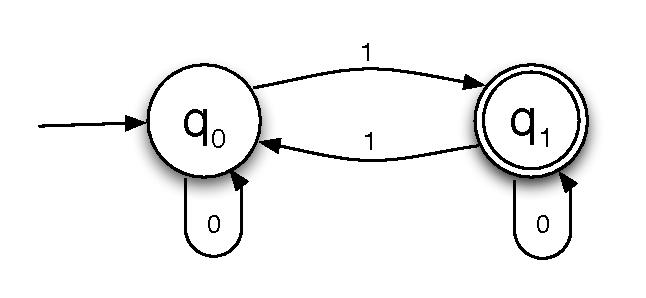
\epsfig{figure=Figures/fig-1-6.eps,width=\textwidth}}
\centerline{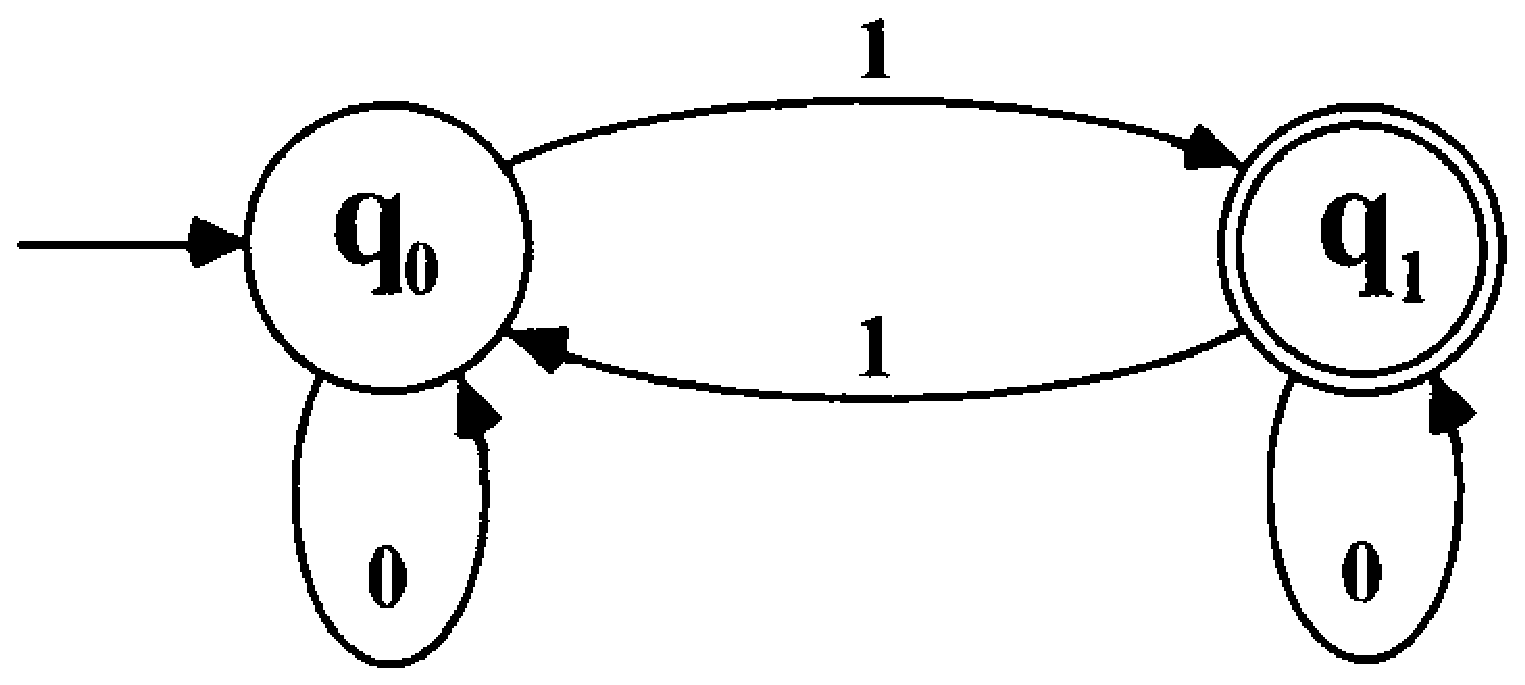
\epsfig{figure=ToFAfigures/fig1-6.eps,width=3in}}
\caption{The DFA discussed in Example 1.7}\label{fig-1.6}
\end{figure}

The functions \texttt{Delta}, \texttt{DeltaBar}, and \texttt{Accept} can be
combined to form a Pascal program that models a DFA. The sample fragments given
in Figures \ref{fig-1.4}, \ref{fig-1.5}, and \ref{fig-1.7} rightly pass the
candidate string as a parameter. A full program would be complicated by several
constraints, including the awkward way in which strings must be handled in
Pascal. To highlight the correspondence between the code modules and the
automata definitions, the program given in Figure \ref{fig-1.8} handles input at
the character level rather than at the word level. The definitions in the
procedure \texttt{Initialize} reflect the structure of the DFA shown in Figure
\ref{fig-1.9}. Invoking this program will produce a response to a single input
word. For example, a typical exchange would be
\begin{align*}
\pmb{cba} & \\
\text{Rejected} & \\
\intertext{Running this program again might produce}
\pmb{cccc} & \\
\text{Accepted} & \\
\end{align*}
This behavior is essentially the same as that of the C program shown
in Figure \ref{fig-1.10}. The succinct coding clearly shows the relationship
between the components of the quintuple for the DFA and the corresponding code.

% Definition 1.14
\begin{dfn}\label{dfn-1.14}
Given an alphabet $\Sigma$, $L$ is a \emph{\Index{language}} over the alphabet
$\Sigma$ iff $L \subseteq \Sigma^*$.
\end{dfn}

A language is a collection of words over some alphabet. If the alphabet is
denoted by $\Sigma$, then a language $L$ over $\Sigma$ is a subset of
$\Sigma^*$. Since $L \subseteq \Sigma^*$, $L$ may be finite or infinite.
Clearly, the words used in the English language are a subset of words over the
Roman alphabet and this collection is therefore a language according to our
definition. Note that a language $L$, in this context, is simply a list of
words; neither syntax nor semantics are involved in the specification of $L$.
Thus, a language as defined by Definition \ref{dfn-1.14} has little of the
structure or relationships one would normally expect of either a natural
language (like English) or a programming language (like Pascal).

% Figure 1.7
\begin{figure}
\begin{verbatim}
function Accept(W:Word):Boolean;
{returns TRUE iff W is accepted by the DFA}
begin
   Accept := DeltaBar(s0, W) in FinalState
end; {Accept}
\end{verbatim}
\caption{A Pascal implementation of a test for acceptance}\label{fig-1.7}
\end{figure}

% Figure 1.8
\begin{figure}
\begin{verbatim}
program DFA(input, output);
{This program tests whether input strings are accepted by the     }
{automaton displayed in Figure 1.9. The program expects input from}
{the keyboard, delimited by a carriage return. No error checking  }
{is done; letters outside ['a' .. 'c'] cause a range error.       }
type
    Sigma = 'a'..'c';
    State = (s0, s1, s2);
var
    TransitionTable : array [State, Sigma] of State;
    FinalState	     : set of State;
function Delta(s : State; c : Sigma) : State;
begin
    Delta := TransitionTable[s,c]
end; { Delta }
function DeltaBar(s : State) : State;
var
    t : State;
begin
    t := s;
    { Step through the keyboard input one letter at a time. }
    while not eoln(input) do
        begin
	    t := Delta(t, input^);
	    get(input)
	end;
    DeltaBar := t
end; { DeltaBar }
function Accept : boolean;
begin
    Accept := DeltaBar(s0) in FinalState
end; { Accept }
procedure Initialize;
begin
    FinalState := [s2];
    { Set up the state transition table. }
    TransitionTable [s0,'a'] := s1; TransitionTable [s0,'b'] := s0;
    TransitionTable [s0,'c'] := s2; TransitionTable [s1,'a'] := s2;
    TransitionTable [s1,'b'] := s0; TransitionTable [s1,'c'] := s0;
    TransitionTable [s2,'a'] := s0; TransitionTable [s2,'b'] := s0;
    TransitionTable [s2,'c'] := s1;
end; { Initialize }
begin { DFA }
    Initialize;
    if Accept then
        writeln(output, 'Accepted')
    else
        writeln(output, 'Rejected')
end. { DFA }
\end{verbatim}
\caption{A Pascal program that emulates the DFA shown in Figure \ref{fig-1.9}}\label{fig-1.8}
\end{figure}

% Figure 1.9
\begin{figure}\index{finite automaton!Pascal implementation}
%\centerline{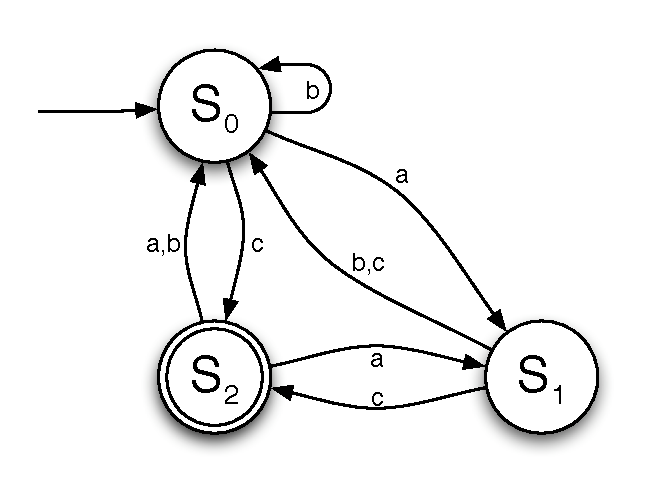
\epsfig{figure=Figures/fig-1-9.eps,width=\textwidth}}
\centerline{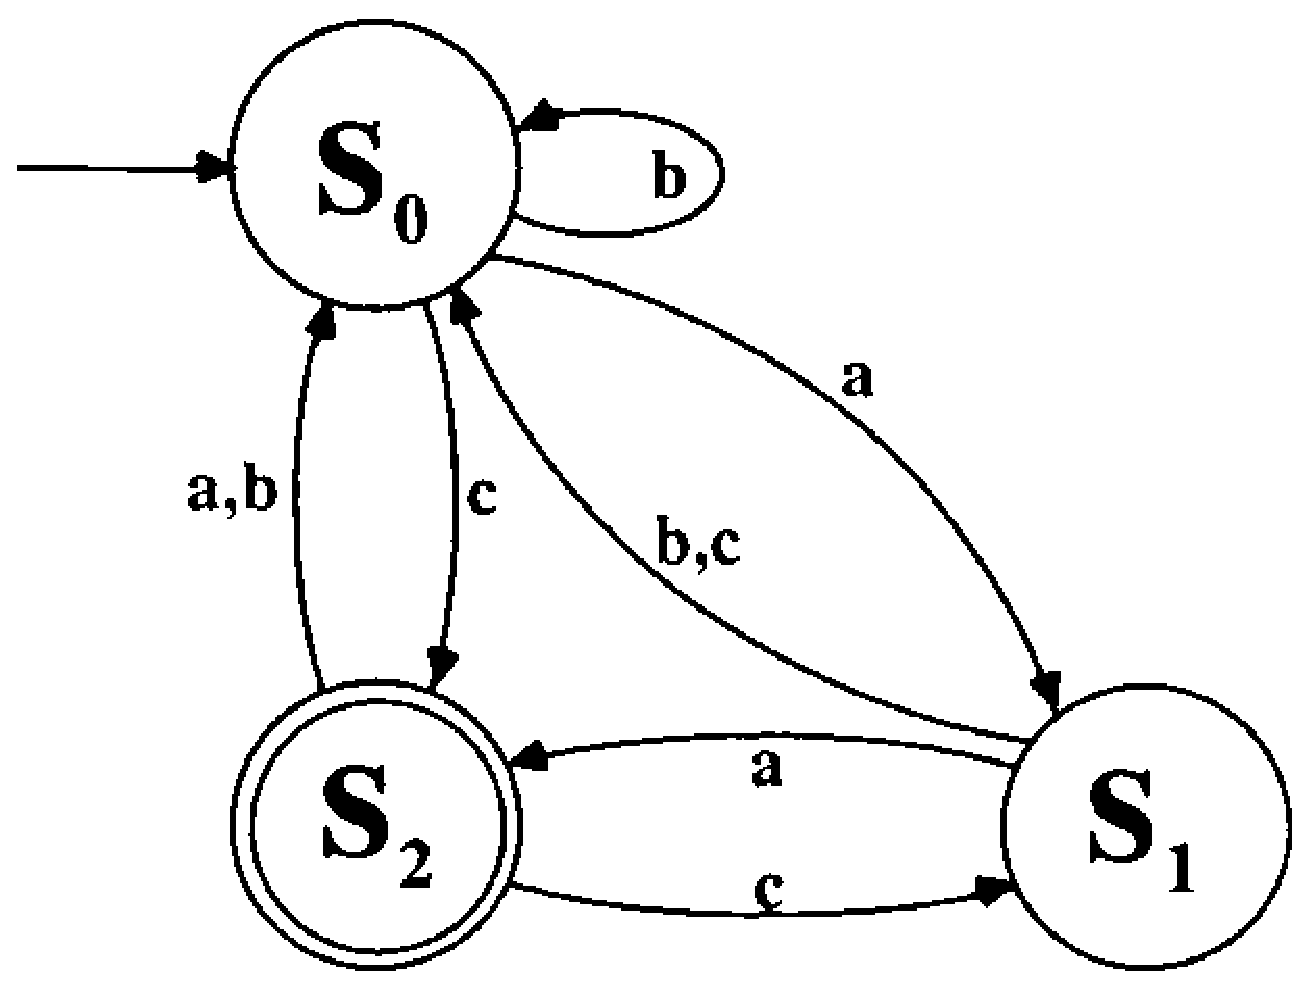
\epsfig{figure=ToFAfigures/fig1-9.eps,width=3in}}
\caption{The DFA emulated by the programs in Figures \ref{fig-1.8} and
\ref{fig-1.10}}\label{fig-1.9}
\end{figure}

\subsection*{Example 1.8}

Some other examples of valid languages are
\begin{enumerate}[i.]
\item $\emptyset$
\item $\{w \in\{\pmb{0},\pmb{1}\}^*\ | \ \ \ |w| > 5\}$
\item $\{\lambda\}$
\item \{$\lambda$, {\bf bilbo}, {\bf frodo}, {\bf samwise}\}
\item $\{x \in \{\pmb{a},\pmb{b}\}^*\ | \ \ \ |x|_{\pmb{a}} = |x|_{\pmb{b}}\}$
\end{enumerate}

% Figure 1.10
\begin{figure}
\begin{verbatim}
# include       <stdio.h>
# define        to_int(c)       ((int) c-(int) 'a')
# define        FINAL_STATE     s_2

enum state { s_0, s_1, s_2 };
/*
** This table implements the state transition function and is indexed by
** the current state and the current input letter.
*/
enum state transition_table[3][3]={ { s_1, s_0, s_2 },
                                    { s_2, s_0, s_0 },
                                    { s_0, s_0, s_1 }};
enum state delta(enum state s, char c) {
        return transition_table[(int) s][to_int(c)];
}
enum state delta_bar(enum state s) {
        enum state t;
        char       c;
	
        t=s;
/*
** Step through the input one letter at a time.
*/
        while ((char) (c = getchar()) != '\n')
              t=delta(t, c);
        return t;
}
main() {
        if (delta_bar(s_0) == FINAL_STATE)
                printf("Accepted\n");
        else
                printf("Rejected\n");
        exit(0);
}
\end{verbatim}
\caption{A C program that emulates the DFA shown in Figure \ref{fig-1.9}}\label{fig-1.10}\index{finite automaton!C implementation}
\end{figure}

The empty language, denoted by $\emptyset$ or $\{\ \ \}$, is different from
$\{\lambda\}$, the language consisting of only the empty word $\lambda$. Whereas
the empty language consists of zero words, the language consisting of $\lambda$
contains one word (which contains zero letters). The distinction is analogous to
an example involving sets of numbers: the set $\{0\}$, containing only the
integer $0$, is still a larger set than the empty set.

Every DFA differentiates between words that do not reach final states and 
words that do. In this sense, each automaton defines a language.

% Definition 1.15
\begin{dfn}\label{dfn-1.15}
Given a DFA $A = \langle\Sigma,S,s_0,\delta,F\rangle$, the \emph{language accepted by}
$A$, denoted $L(A)$, is defined to be 
$$L(A) = \{w \in \Sigma^*\ | \ \DBAR(s_0, w) \in F\}$$
\end{dfn}

$L(A)$, the language accepted by a finite automaton $A$, is the set of all words
$w$ from $\Sigma^*$ for which $\DBAR(s_0, w) \in F$. In order for a
word $w$ to be contained in $L(B)$, the path through the finite automaton B, as
determined by the letters in $w$, must lead from the start state to one of the
final states.

For deterministic finite automata, the path for a given word $w$ is unique:
there is only one path since, at any given state in the automaton, there is
exactly one transition for each $a \in \Sigma$. This is not necessarily the case
for another variety of finite automaton, the \emph{nondeterministic} finite
automaton, as will be seen in Chapter \ref{ch-4}.

% Definition 1.16
\begin{dfn}\label{dfn-1.16}\index{finite automaton definable}
Given an alphabet $\Sigma$, a language $L \subseteq \Sigma^*$ is 
\emph{finite automaton definable} (FAD) iff there exists some DFA
$B =\ \langle\Sigma,S,s_0,\delta,F\rangle$, such that $L = L(B)$.
\end{dfn}

The set of all words over $\{\pmb{0,1}\}$ that contain an odd number of
\pmb{1}s is finite
automaton definable, as evidenced by the automaton in Example 1.7,
which accepts exactly this set of words.

\section{Examples of Finite Automata}\label{sec-1.3}

This section illustrates the definitions of the quintuples and the state
transition diagrams for some nontrivial automata. The following example and
Example 1.11 deal with the recognition of tokens, an important issue in
the construction of compilers.

\subsection*{Example 1.9}\index{ASCII alphabet}

The set of FORTRAN identifiers is a finite automaton definable language. This
statement can be proved by verifying that the following machine accepts the set
of all valid FORTRAN 66 identifiers. These identifiers, which represent
variable, subroutine, and array names, can contain from 1 to 6 (nonblank)
characters, must begin with an alphabetic character, can be followed by up to 5
letters or digits, and may have embedded blanks. In this example, we have
ignored the difference between capital and lowercase letters,
and $\diamond$ represents a blank.\index{blank symbol}

\begin{align*}
\Sigma &=\text{ ASCII} \\
\Gamma &=\text{ ASCII} - \{\pmb{a},\pmb{b},\pmb{c,}\ldots\pmb{x},\pmb{y},\pmb{z},
	\pmb{0},\pmb{1},\pmb{2},\pmb{3},\pmb{4},\pmb{5},\pmb{6},\pmb{7},\pmb{8},
	\pmb{9},\diamond\} \\
S &= \{s_0,s_1,s_2,s_3,s_4,s_5,s_6,s_7\} \\
s_0 &= s_0
\end{align*}

\begin{center}
\begin{tabular}{c|ccccccccc}
$\delta$ & $\pmb{a}$ & $\pmb{b}$ & $\pmb{c}\ldots\pmb{y}$ & $\pmb{z}$ & $\pmb{0}$
	& $\pmb{1}\ldots\pmb{8}$ & $\pmb{9}$ & $\diamond$ & $\Gamma$ \\
\hline
$s_0$ & $s_1$ & $s_1$ & $s_1\ldots s_1$ & $s_1$ & $s_7$ & $s_7\ldots s_7$
	& $s_7$ & $s_0$ & $s_7$ \\
$s_1$ & $s_2$ & $s_2$ & $s_2\ldots s_2$ & $s_2$ & $s_2$ & $s_2\ldots s_2$
	& $s_2$ & $s_1$ & $s_7$ \\ 
$s_2$ & $s_3$ & $s_3$ & $s_3\ldots s_3$ & $s_3$ & $s_3$ & $s_3\ldots s_3$
	& $s_3$ & $s_2$ & $s_7$ \\
$s_3$ & $s_4$ & $s_4$ & $s_4\ldots s_4$ & $s_4$ & $s_4$ & $s_4\ldots s_4$
	& $s_4$ & $s_3$ & $s_7$ \\
$s_4$ & $s_5$ & $s_5$ & $s_5\ldots s_5$ & $s_5$ & $s_5$ & $s_5\ldots s_5$
	& $s_5$ & $s_4$ & $s_7$ \\
$s_5$ & $s_6$ & $s_6$ & $s_6\ldots s_6$ & $s_6$ & $s_6$ & $s_6\ldots s_6$
	& $s_6$ & $s_5$ & $s_7$ \\
$s_6$ & $s_7$ & $s_7$ & $s_7\ldots s_7$ & $s_7$ & $s_7$ & $s_7\ldots s_7$
	& $s_7$ & $s_6$ & $s_7$ \\
$s_7$ & $s_7$ & $s_7$ & $s_7\ldots s_7$ & $s_7$ & $s_7$ & $s_7\ldots s_7$
	& $s_7$ & $s_7$ & $s_7$
\end{tabular}
$$F = \{s_1,s_2,s_3,s_4,s_5,s_6\}$$
\end{center}

The entries under the column labeled $\Gamma$ show the transitions taken for
each member of the set $\Gamma$. The state transition diagram of the machine
corresponding to this quintuple is displayed in Figure \ref{fig-1.11}. Note
that, while each of the 26 letters transition from $s_0$ to $s_1$, a single
arrow labeled \pmb{a}-\pmb{z} is sufficient to denote all these transitions. Similarly, the
transition labeled $\Sigma$ from $s_7$ indicates that every element of the
alphabet follows the same path.

% Figure 1.11
\begin{figure}
\centerline{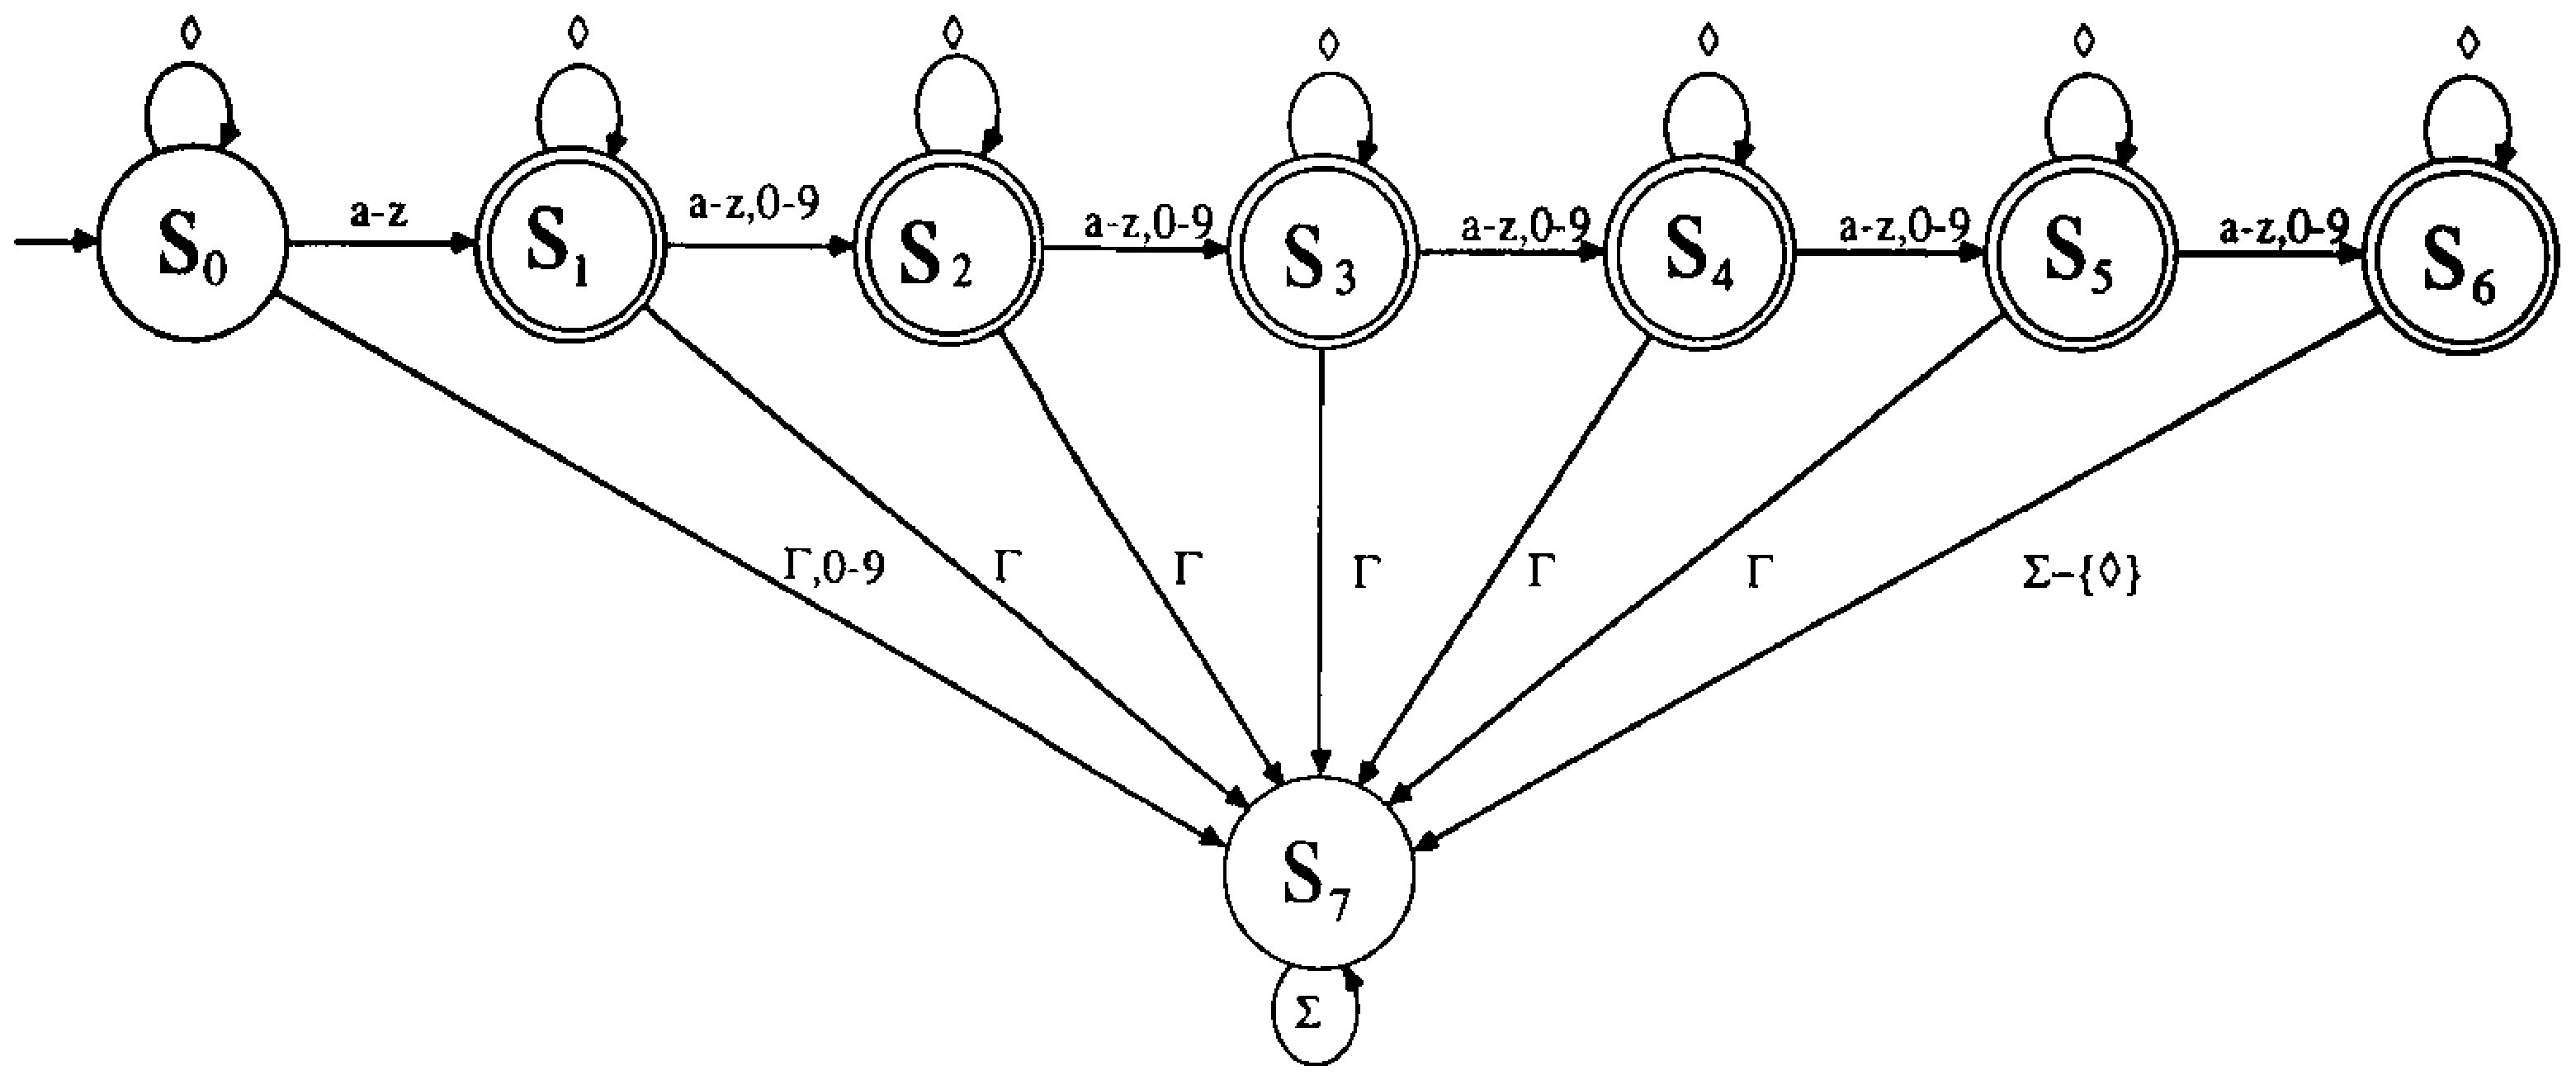
\epsfig{figure=ToFAfigures/fig1-11.eps,width=6.5in}}
\caption{A DFA that recognizes valid FORTRAN identifiers}\label{fig-1.11}
\end{figure}

% Figure 1.12
\begin{figure}
\centerline{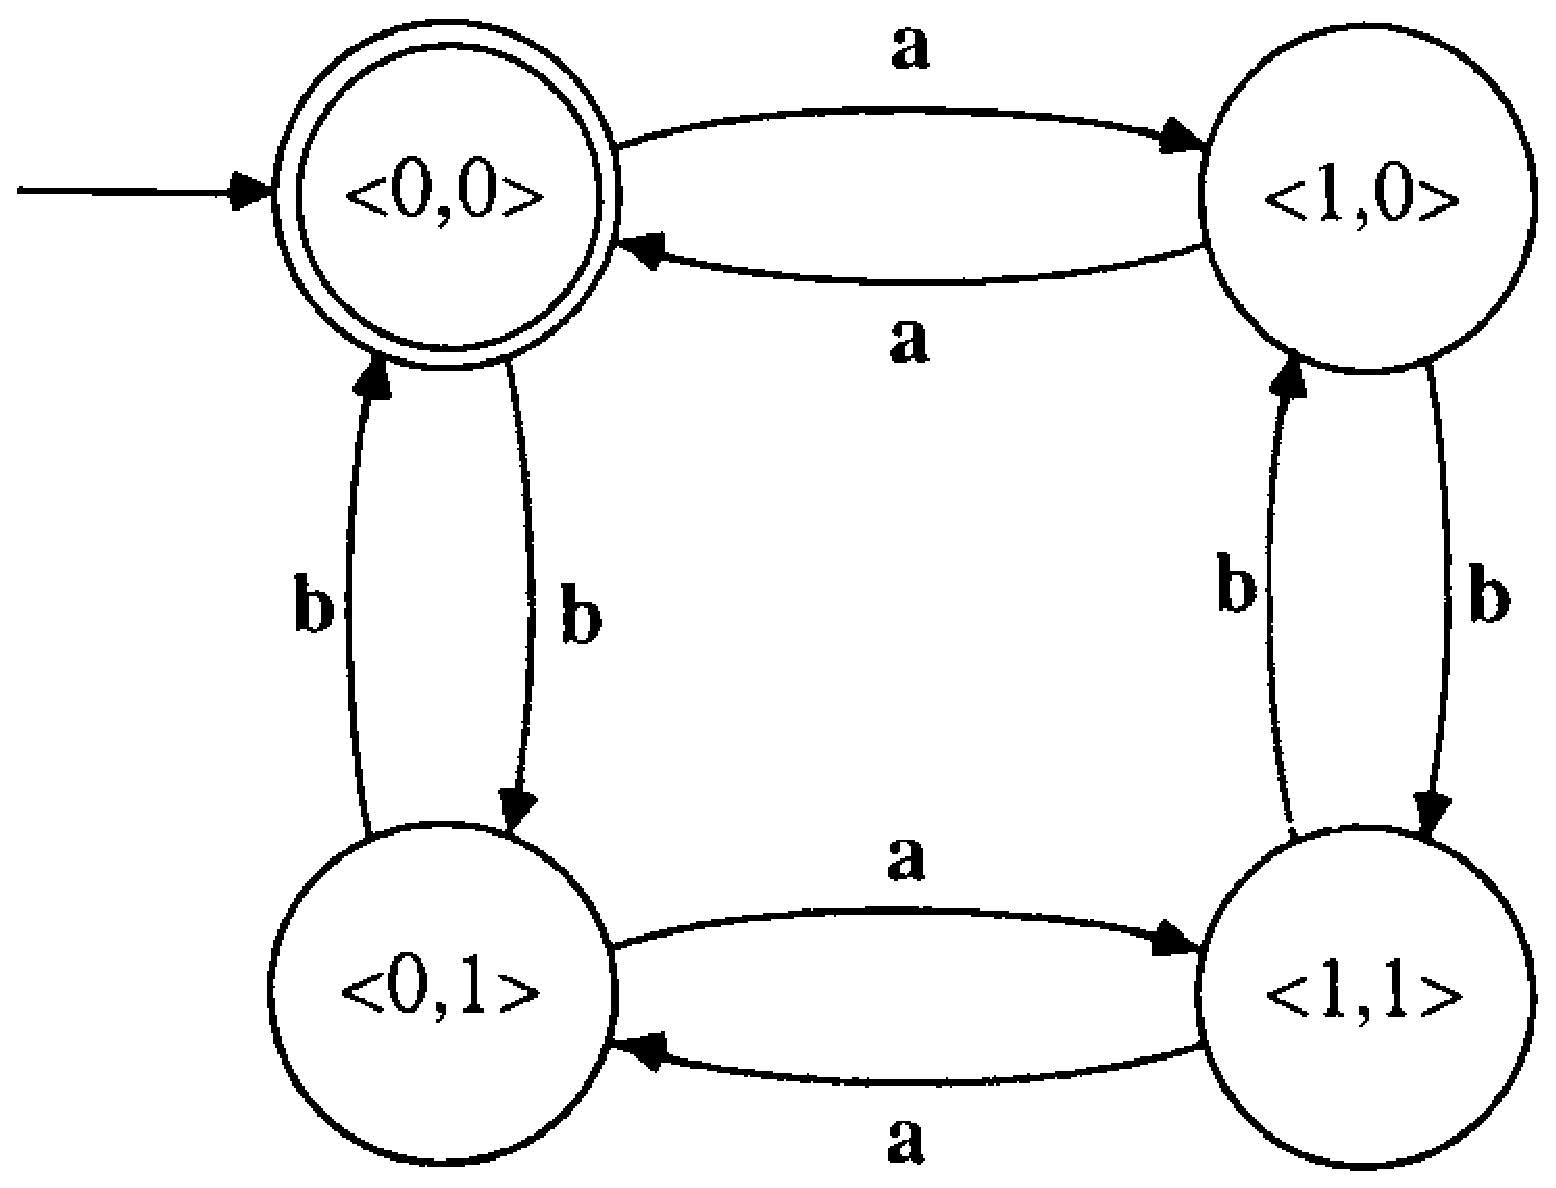
\epsfig{figure=ToFAfigures/fig1-12.eps,width=2.7in}}
\caption{The DFA $M$ discussed in Example 1.10}\label{fig-1.12}
\end{figure}

\subsection*{Example 1.10}

The DFA $M$ shown in Figure \ref{fig-1.12} accepts only those strings that have an even
number of $\pmb{b}$s and an even number of $\pmb{a}$s. Thus
$$L(M) = \{x \in \{\pmb{a},\pmb{b}\}^* \ | \ \ \ |x|_{\pmb{a}} \equiv 0 \bmod 2 \wedge
	|x|_{\pmb{b}} \equiv 0\bmod 2\}$$
The corresponding quintuple for $M = \langle\Sigma,S,s_0,\delta,F\rangle$ has the
following components:
\begin{align*}
\Sigma &= \{\pmb{a},\pmb{b}\} \\
S &= \{\langle 0,0\rangle,\langle 0,1\rangle,\langle 1,0\rangle,\langle 1,1\rangle\} \\
s_0 &= \langle 0,0\rangle
\end{align*}

\begin{center}
\begin{tabular}{c|cc}
$\delta$ & $\pmb{a}$ & $\pmb{b}$ \\
\hline
$\langle 0,0\rangle$ & $\langle 1,0\rangle$ & $\langle 0,1\rangle$ \\
$\langle 0,1\rangle$ & $\langle 1,1\rangle$ & $\langle 0,0\rangle$ \\
$\langle 1,0\rangle$ & $\langle 0,0\rangle$ & $\langle 1,1\rangle$ \\
$\langle 1,1\rangle$ & $\langle 0,1\rangle$ & $\langle 1,0\rangle$
\end{tabular}
$$F=\{\langle 0,0\rangle\}$$
\end{center}
Note that the transition function can be succinctly specified by
$$\delta(\langle i,j\rangle,\pmb{a}) = \langle 1-i,j\rangle\text{ and }\delta(
	\langle i,j\rangle,\pmb{b}) = \langle i,1-j\rangle\text{ for all } i,j
	\in \{0,1\}$$
See the exercises for some other problems involving congruence modulo 2.

\subsection*{Example 1.11}

Consider a typical set of all real number constants in modified scientific
notation format described by the BNF in Table \ref{tbl-1.1}.\index{BNF}

This set of productions defines real number constants like $\pmb{+192.}$, since
\begin{align*}
\<\text{real constant}\> &\Rightarrow \<\text{integer}\>\pmb{.} \\
\<\text{integer}>. &\Rightarrow \<\text{sign}\>\<\text{natural}\>\pmb{.} \\
\<\text{sign}\>\<\text{natural}\>. &\Rightarrow \pmb{+} \<\text{natural}\>\pmb{.} \\
\pmb{+}\<\text{natural}\>. &\Rightarrow \pmb{+}\<\text{digit}\>\<\text{natural}\>\pmb{.} \\
\pmb{+}<\text{digit}\>\<\text{natural}>. &\Rightarrow \pmb{+1}\<\text{natural}\>\pmb{.} \\
\pmb{+1}\<\text{natural}\>. &\Rightarrow \pmb{+1}\<\text{digit}\>\<\text{natural}\>\pmb{.} \\
\pmb{+1}\<\text{digit}\>\<\text{natural}\>. &\Rightarrow\pmb{+1}\<\text{digit}\>\<\text{digit}\>\pmb{.} \\
\pmb{+1}\<\text{digit}\>\<\text{digit}\>. &\Rightarrow\pmb{+1}\<\text{digit}\>\pmb{2.} \\
\pmb{+1}\<\text{digit}\>\pmb{2.}&\Rightarrow \pmb{+192.}
\end{align*}
Other possibilities are
\begin{center}
\begin{tabular}{l}
$\pmb{1}$ \\
$\pmb{3.1415}$ \\
$\pmb{2.718281828}$ \\
$\pmb{27.}$ \\
$\pmb{42.42}$ \\
$\pmb{1.0E-32}$
\end{tabular}
\end{center}
while the following strings do not qualify:
\begin{center}
\begin{tabular}{l}
$\pmb{.01}$ \\
$\pmb{1.+1}$ \\
$\pmb{8.E-10}$
\end{tabular}
\end{center}

% table was edited to fix several errors on 12/29/17, and then moved
% here to prevent it being placed ABOVE Example 1.10...
% Placement is still not great, but it's better than it was.
% Table 1.1
\begin{table}\caption{For Example 1.11}\label{tbl-1.1}
\begin{center}\begin{tabular}{rcl}
\hline
\<sign\> & ::= & $ \pmb + | \pmb -$ \\
\<digit\> & ::= & $ \pmb 0|\pmb 1|\pmb 2|\pmb 3|\pmb 4|\pmb 5|\pmb 6|\pmb 7|\pmb 8|\pmb 9$ \\
\<natural\> & ::= & \<\text{digit}\>$|$\<digit\>\<natural\> \\
\<integer\> & ::= & \<natural\>$|$\<sign\>\<natural\> \\
\<real constant\> & ::= & \<integer\> \ \ \ \ \ \ \ \ \ \ \ \ \ \ \ \ \ \ \ \ \ \ \ \ $|$ \\
 & &\ \ \<integer\>\pmb{.}  \ \ \ \ \ \ \ \ \ \ \ \ \ \ \ \ \ \ \ \ \ $|$ \\
 & &\ \ \<integer\>\pmb{.}\<natural\> \ \,$|$ \\
 & &\ \ \<integer\>\pmb{.}\<natural\>\pmb{E}\<integer\> \\
\hline
\end{tabular}\end{center}
\end{table}

The set of all real number constants that can be derived from the productions
given in Table \ref{tbl-1.1} is a FAD language. Let $R$ be the deterministic
finite automaton defined below. The corresponding state transition diagram is
given in Figure \ref{fig-1.13}.
\begin{align*}
\Sigma &= \{\pmb{0},\pmb{1},\pmb{2},\pmb{3},\pmb{4},\pmb{5},\pmb{6},\pmb{7},
	\pmb{8},\pmb{9},\pmb{+},\pmb{-},\pmb{E},\pmb{.}\} \\
S &= \{s_0,s_1,s_2,s_3,s_4,s_5,s_6,s_7,s_8\} \\
s_0 &= s_0
\end{align*}

\begin{center}
\begin{tabular}{c|cccccccccccccc}
$\delta$ & $\pmb{0}$ & $\pmb{1}$ & $\pmb{2}$ & $\pmb{3}$ & $\pmb{4}$ & $\pmb{5}$
	& $\pmb{6}$ & $\pmb{7}$ & $\pmb{8}$ & $\pmb{9}$ & $\pmb{+}$ & $\pmb{-}$
	& $\pmb{E}$ & $\pmb{.}$ \\
\hline
$s_0$ & $s_2$ & $s_2$ & $s_2$ & $s_2$ & $s_2$ & $s_2$ & $s_2$ & $s_2$ & $s_2$
	& $s_2$ & $s_1$ & $s_1$ & $s_7$ & $s_7$ \\
$s_1$ & $s_2$ & $s_2$ & $s_2$ & $s_2$ & $s_2$ & $s_2$ & $s_2$ & $s_2$ & $s_2$
	& $s_2$ & $s_7$ & $s_7$ & $s_7$ & $s_7$ \\
$s_2$ & $s_2$ & $s_2$ & $s_2$ & $s_2$ & $s_2$ & $s_2$ & $s_2$ & $s_2$ & $s_2$
	& $s_2$ & $s_7$ & $s_7$ & $s_7$ & $s_3$ \\
$s_3$ & $s_8$ & $s_8$ & $s_8$ & $s_8$ & $s_8$ & $s_8$ & $s_8$ & $s_8$ & $s_8$
	& $s_8$ & $s_7$ & $s_7$ & $s_7$ & $s_7$ \\
$s_4$ & $s_5$ & $s_5$ & $s_5$ & $s_5$ & $s_5$ & $s_5$ & $s_5$ & $s_5$ & $s_5$
	& $s_5$ & $s_6$ & $s_6$ & $s_7$ & $s_7$ \\
$s_5$ & $s_5$ & $s_5$ & $s_5$ & $s_5$ & $s_5$ & $s_5$ & $s_5$ & $s_5$ & $s_5$
	& $s_5$ & $s_7$ & $s_7$ & $s_7$ & $s_7$ \\
$s_6$ & $s_5$ & $s_5$ & $s_5$ & $s_5$ & $s_5$ & $s_5$ & $s_5$ & $s_5$ & $s_5$
	& $s_5$ & $s_7$ & $s_7$ & $s_7$ & $s_7$ \\
$s_7$ & $s_7$ & $s_7$ & $s_7$ & $s_7$ & $s_7$ & $s_7$ & $s_7$ & $s_7$ & $s_7$
	& $s_7$ & $s_7$ & $s_7$ & $s_7$ & $s_7$ \\
$s_8$ & $s_8$ & $s_8$ & $s_8$ & $s_8$ & $s_8$ & $s_8$ & $s_8$ & $s_8$ & $s_8$
	& $s_8$ & $s_7$ & $s_7$ & $s_4$ & $s_7$
\end{tabular}
$$F = \{s_2,s_3,s_5,s_8\}$$
\end{center}

The language accepted by $R$, that is $L(R)$, is exactly the set of all real
number constants in modified scientific notation format described by the BNF in
Table \ref{tbl-1.1}.

% Figure 1.13
\begin{figure}%]tbh]
\centerline{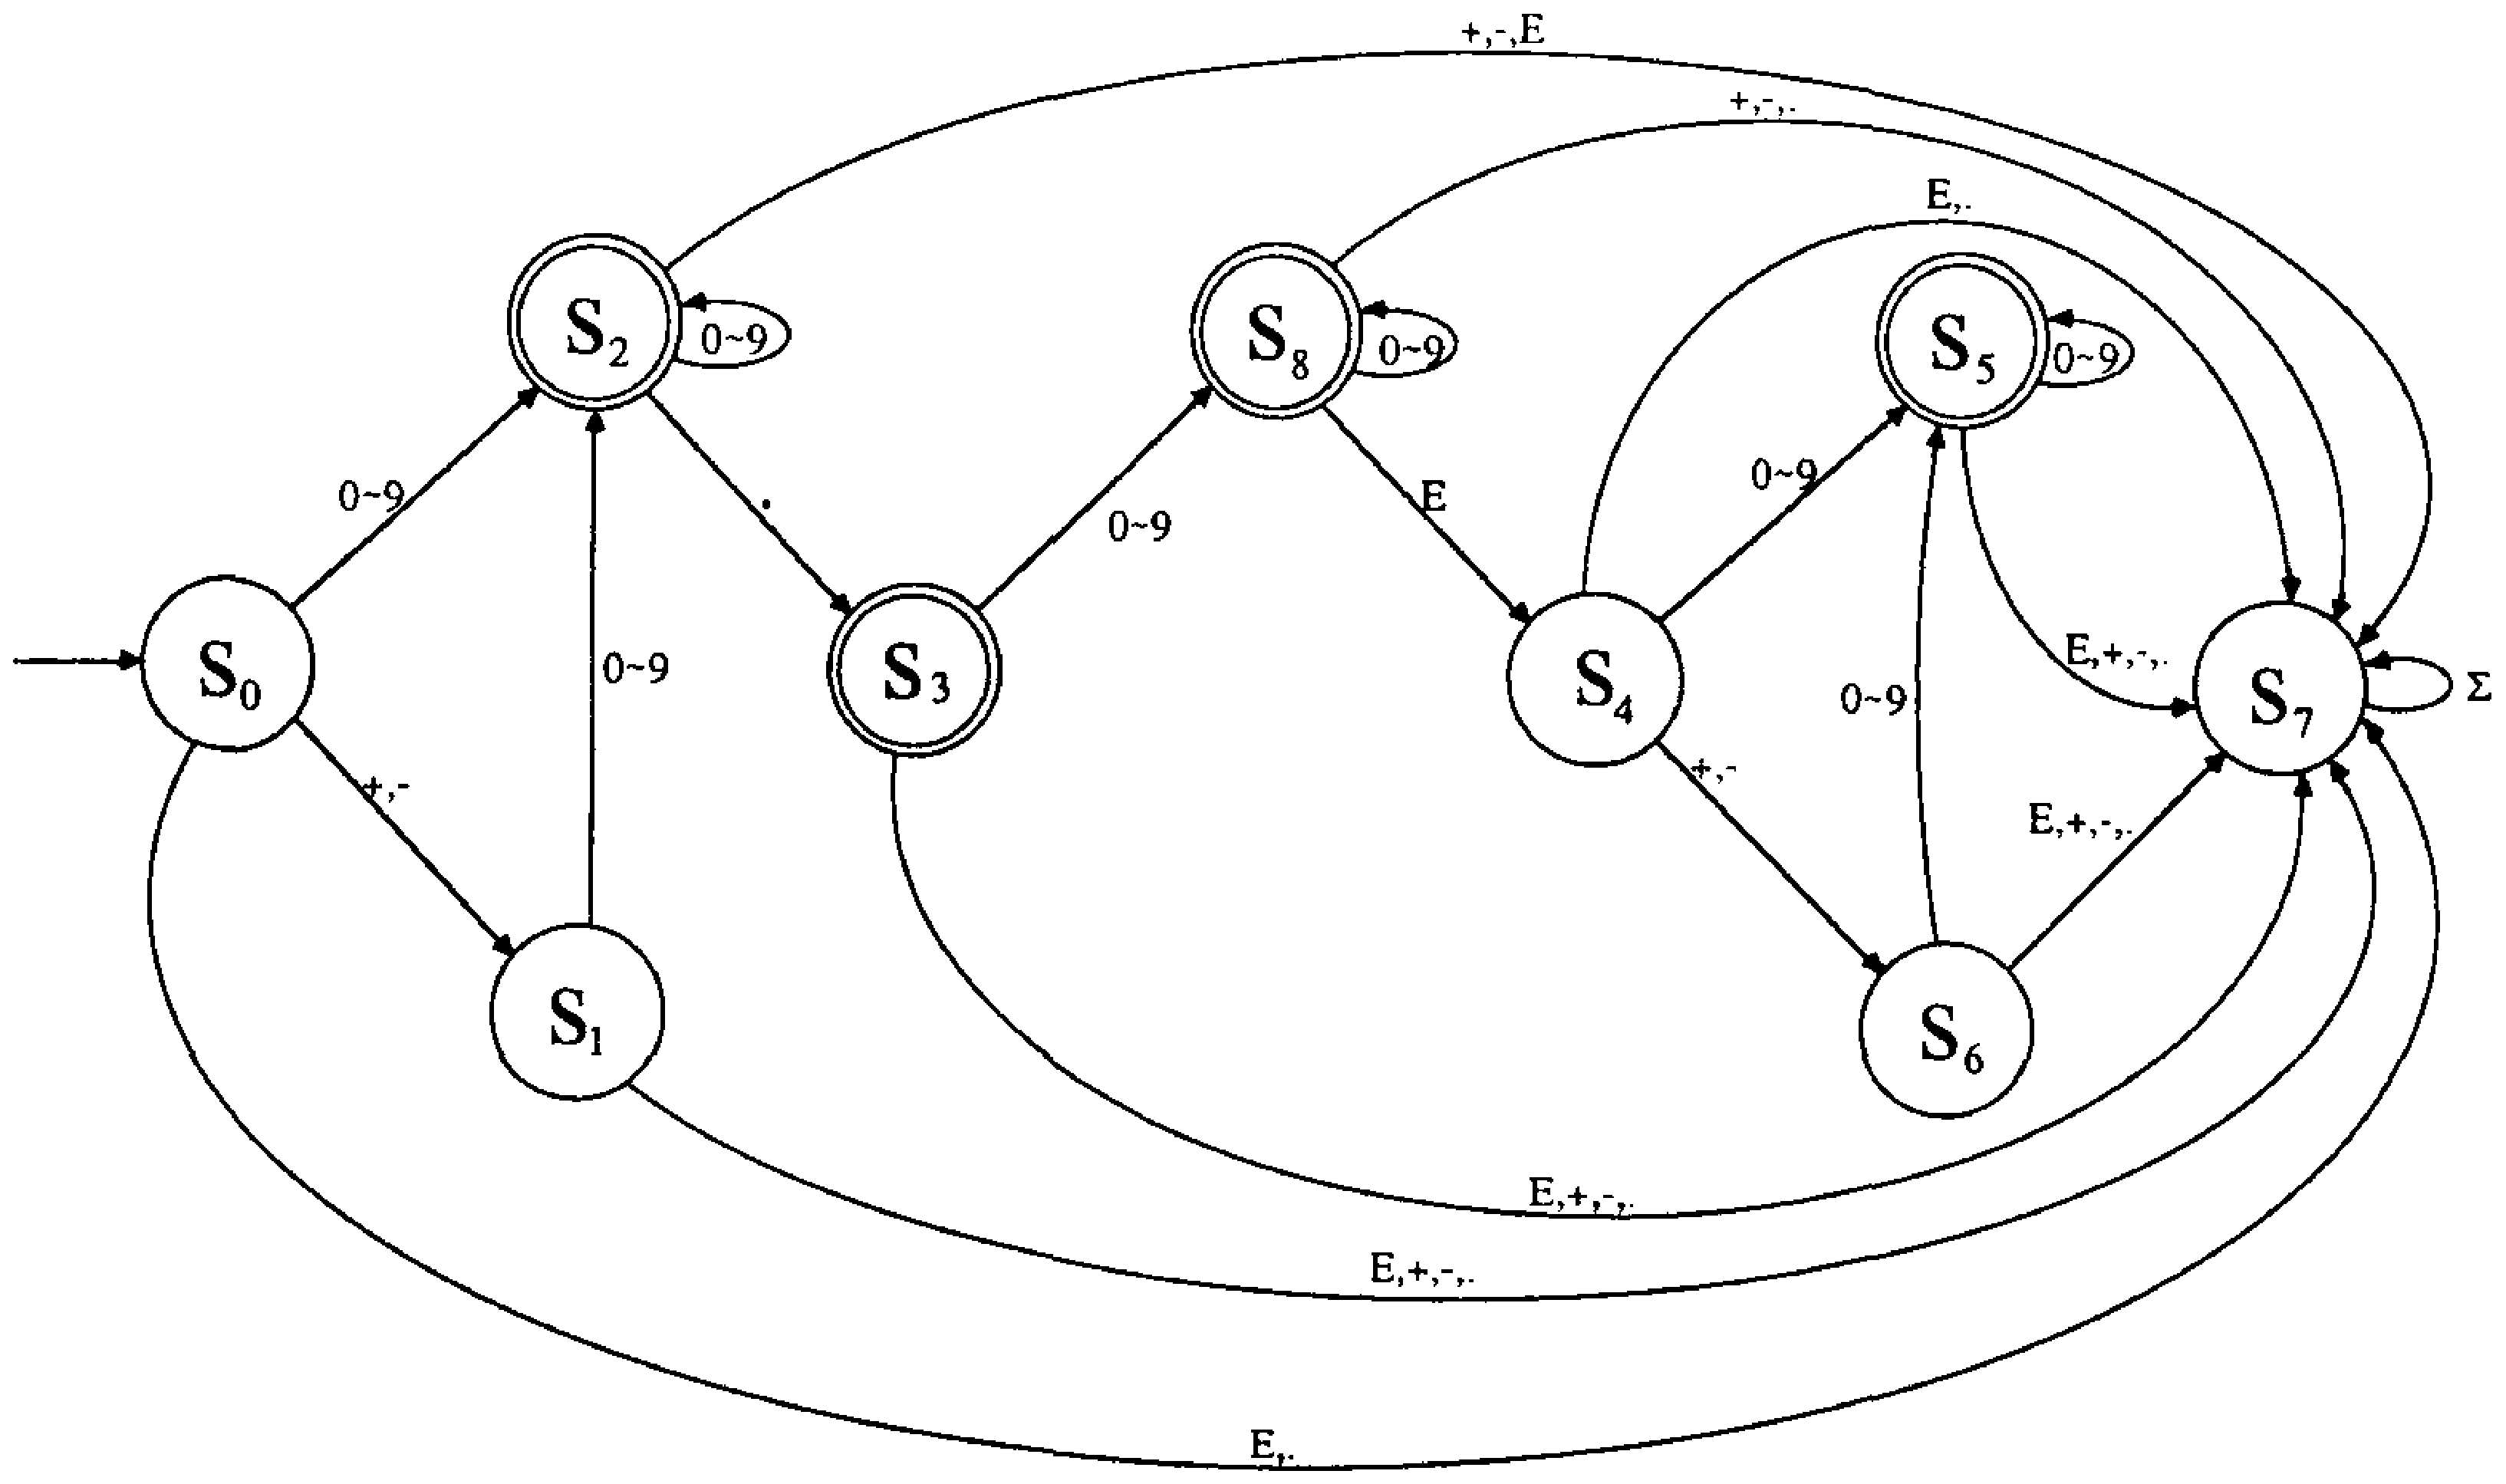
\epsfig{figure=ToFAfigures/fig1-13.eps,width=6.5in}}
\caption{A DFA that recognizes real number constants}\label{fig-1.13}
\end{figure}

For example, let $x = \pmb{3.1415}$:
\begin{align*}
\DBAR(s_0,x) &= \DBAR(s_0,\pmb{3.1415}) \\
&= \DBAR(\delta(s_0,\pmb{3}),\pmb{.1415}) \\
&= \DBAR(s_2,\pmb{.1415}) \\
&= \DBAR(\delta(s_2,\pmb{.}),\pmb{1415}) \\
&= \DBAR(s_3,\pmb{1415}) \\
&= \DBAR(\delta(s_3,\pmb{1}),\pmb{415}) \\
&= \DBAR(s_8,\pmb{415}) \\
&= \DBAR(\delta(s_8,\pmb{4}),\pmb{15}) \\
&= \DBAR(s_8,\pmb{15}) \\
&= \DBAR(\delta(s_8,\pmb{1}),\pmb{5}) \\
&= \DBAR(s_8,\pmb{5}) \\
&= \delta(s_8,\pmb{5}) \\
&= s_8
\end{align*}
$s_8 \in F$, and therefore $\pmb{3.1415}\in L(R)$.

While many important classes of strings such as numerical constants (Example
1.11) and identifiers (Example 1.9) are FAD, not all languages
that can be described by BNF can be recognized by DFAs. These limitations will
be investigated in Chapters \ref{ch-8} and \ref{ch-9}, and a more capable type
of automaton will be defined in Chapter \ref{ch-10}.

\section{Circuit Implementation of Finite Automata}\label{sec-1.4}\index{finite automaton!circuit implementation}

Now that we have described the mathematical nature of deterministic finite
automata, let us turn to the physical implementation of such devices. We will
investigate the sort of physical components that actually go into the ``brain''
of, say, a vending machine. Recall that the basic building blocks of digital
logic circuits are {\emph{\Index{logic gates}}; using $\pmb{0}$ or {\bf False}
to represent a low voltage (ground) and $\pmb{1}$ or {\bf True} to represent a
higher voltage (often +5 volts), the basic gates have the truth tables shown in
Figure \ref{fig-1.14}.

Since our DFA will examine one letter at a time, we will generally need some
type of timing mechanism, which will be regulated by a
\emph{\Index{clock pulse}}; we will read one letter per pulse and allow enough
interim time for transient signals to propagate through our network as we change
states and move to the next letter on the input tape. The clock pulse will
alternate between high and low voltages, as shown in Figure \ref{fig-1.15}.
For applications such as vending machines, the periodic clock pulse would be
replaced by a device that pulsed whenever a new input (such as the insertion of
a coin) was detected.

% Figure 1.14
\begin{figure}
\centerline{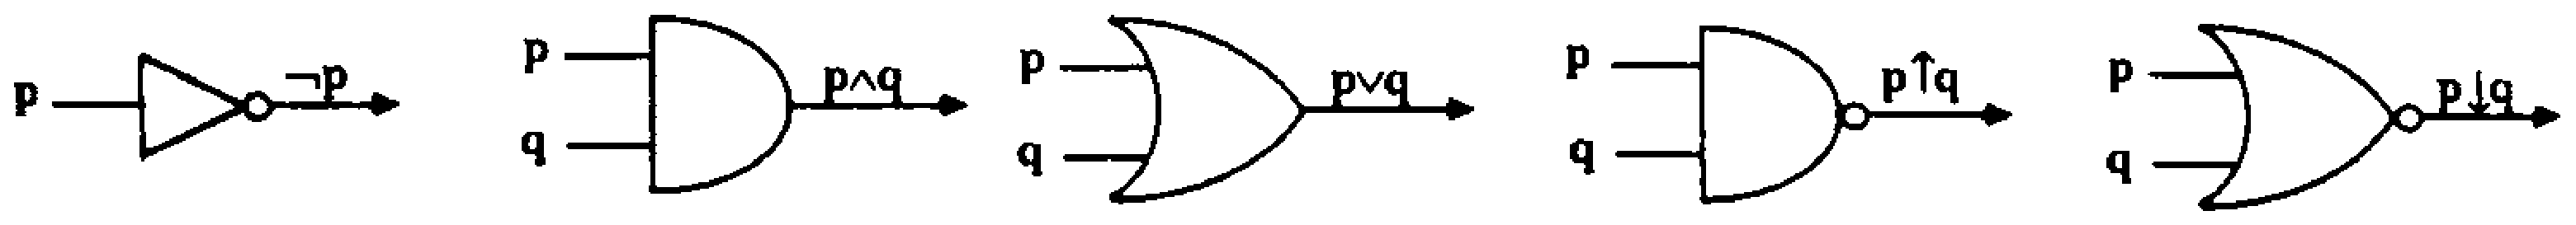
\epsfig{figure=ToFAfigures/fig1-14.eps,width=5.7in}}
\begin{center}
\begin{tabular}{ccccc}
%\fbox{IMAGE} & \fbox{IMAGE} & \fbox{IMAGE} & \fbox{IMAGE} & \fbox{IMAGE} \\
NOT gate & AND gate & OR gate & NAND gate & NOR gate \\
{
\begin{tabular}[b]{c|c}
$p$ & $\neg p$ \\
\hline
$\pmb{1}$ & $\pmb{0}$ \\
$\pmb{0}$ & $\pmb{1}$
\end{tabular}
} & {
\begin{tabular}{cc|c}
$p$ & $q$ & $p\wedge q$ \\
\hline
$\pmb{1}$ & $\pmb{1}$ & $\pmb{1}$ \\
$\pmb{1}$ & $\pmb{0}$ & $\pmb{0}$ \\
$\pmb{0}$ & $\pmb{1}$ & $\pmb{0}$ \\
$\pmb{0}$ & $\pmb{0}$ & $\pmb{0}$
\end{tabular}
} & {
\begin{tabular}{cc|c}
$p$ & $q$ & $p\vee q$ \\
\hline
$\pmb{1}$ & $\pmb{1}$ & $\pmb{1}$ \\
$\pmb{1}$ & $\pmb{0}$ & $\pmb{1}$ \\
$\pmb{0}$ & $\pmb{1}$ & $\pmb{1}$ \\
$\pmb{0}$ & $\pmb{0}$ & $\pmb{0}$
\end{tabular}
} & {
\begin{tabular}{cc|c}
$p$ & $q$ & $p \uparrow q$ \\
\hline
$\pmb{1}$ & $\pmb{1}$ & $\pmb{0}$ \\
$\pmb{1}$ & $\pmb{0}$ & $\pmb{1}$ \\
$\pmb{0}$ & $\pmb{1}$ & $\pmb{1}$ \\
$\pmb{0}$ & $\pmb{0}$ & $\pmb{1}$
\end{tabular}
} & {
\begin{tabular}{cc|c}
$p$ & $q$ & $p \downarrow q$ \\
\hline
$\pmb{1}$ & $\pmb{1}$ & $\pmb{0}$ \\
$\pmb{1}$ & $\pmb{0}$ & $\pmb{0}$ \\
$\pmb{0}$ & $\pmb{1}$ & $\pmb{0}$ \\
$\pmb{0}$ & $\pmb{0}$ & $\pmb{1}$
\end{tabular}
}
\end{tabular}
\end{center}
\caption{Common logic gates and their truth tables}\label{fig-1.14}
\end{figure}

% Figure 1.15
\begin{figure}
\centerline{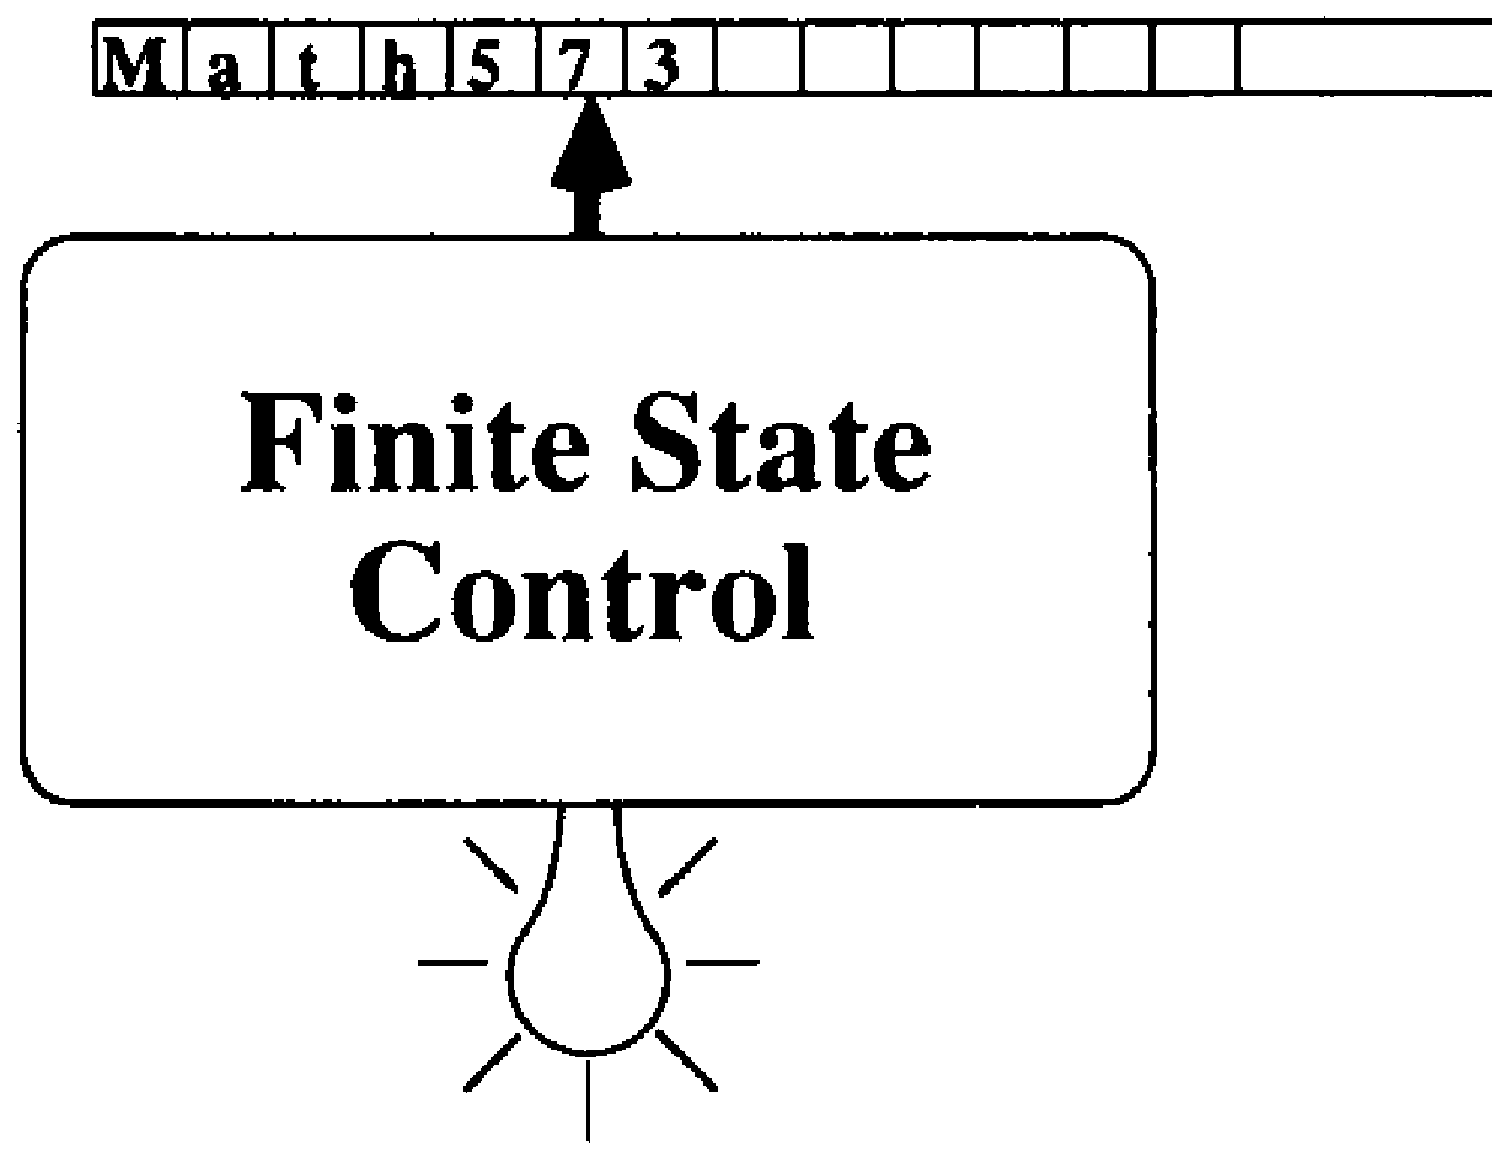
\epsfig{figure=ToFAfigures/fig1-1.eps,width=4in}}
\caption{A typical clock pulse pattern for latched circuits}\label{fig-1.15}
\end{figure}

We need to retain the present status of the network (current state, letter, and
so forth) as we move on to the next input symbol. This is achieved through the
use of a \emph{\Index{D flip-flop}} (D stands for data or delay), which uses
NAND gates and the clock signal to store the current value of, say, \emph{$p'$},
between clock pulses. The symbol for a D flip-flop (sometimes called a
\emph{\Index{latch}}) is shown in Figure \ref{fig-1.16}, along with the actual
gates that comprise the circuit.

The output, $p$ and $\neg p$, will reflect the value of the input signal $p'$
\emph{only} after the high clock pulse is received and will retain that value after the
clock drops to low (even if $p'$ subsequently changes) until the next clock
pulse comes along, at which time the output will reflect the new current value
of $p'$. This is best illustrated by referring to the NAND truth table and
tracing the changes in the circuit. Begin with clock $= p = p' = \pmb{0}$ and 
$\neg p = \pmb{1}$, and verify that the circuit is stable. Now assume that $p'$
changes to $\pmb{1}$, and note that, although some internal values may change,
$p$ and $\neg p$ remain at $\pmb{0}$ and $\pmb{1}$, respectively; the old value
of $p'$ has been ``remembered'' by the D flip-flop. Contrast this with the
behavior when we strobe the clock: assume that the clock now also changes to
$\pmb{1}$ so that we now have clock $=p=p'=\pmb{1}$, and $p=\pmb{0}$. When the
signal propagates through the network, we find that $p$ and $\neg p$ have
changed to reflect the new value of $p'$; clock $=p=p'=\pmb{1}$, and $\neg p=
\pmb{0}$.

We will also have to represent the letters of our input alphabet by high and low
voltages (that is, combinations of $\pmb{0}$s and $\pmb{1}$s). The \index{ASCII alphabet}ASCII alphabet,
for example, is quite naturally represented by 8 bits, 
$\pmb{a}_1\pmb{a}_2\pmb{a}_3\pmb{a}_4\pmb{a}_5\pmb{a}_6\pmb{a}_7\pmb{a}_8$,
where $\pmb{B}$, for example, has the bit pattern $\pmb{01000010}$ (binary 66).
One of these bit patterns should be reserved for indicating the end of our input
string \<EOS\>. Our convention will be to reserve binary zero for this role,
which means our ASCII end of string symbol would be $\pmb{00000000}$ (or NULL).
In actual applications using the ASCII alphabet, however, a more appropriate
choice for \<EOS\> might be $\pmb{00001101}$ (a carriage return) or
$\pmb{00001010}$ (a line feed) or $\pmb{00100000}$ (a space).

% Figure 1.16
\begin{figure}
\centerline{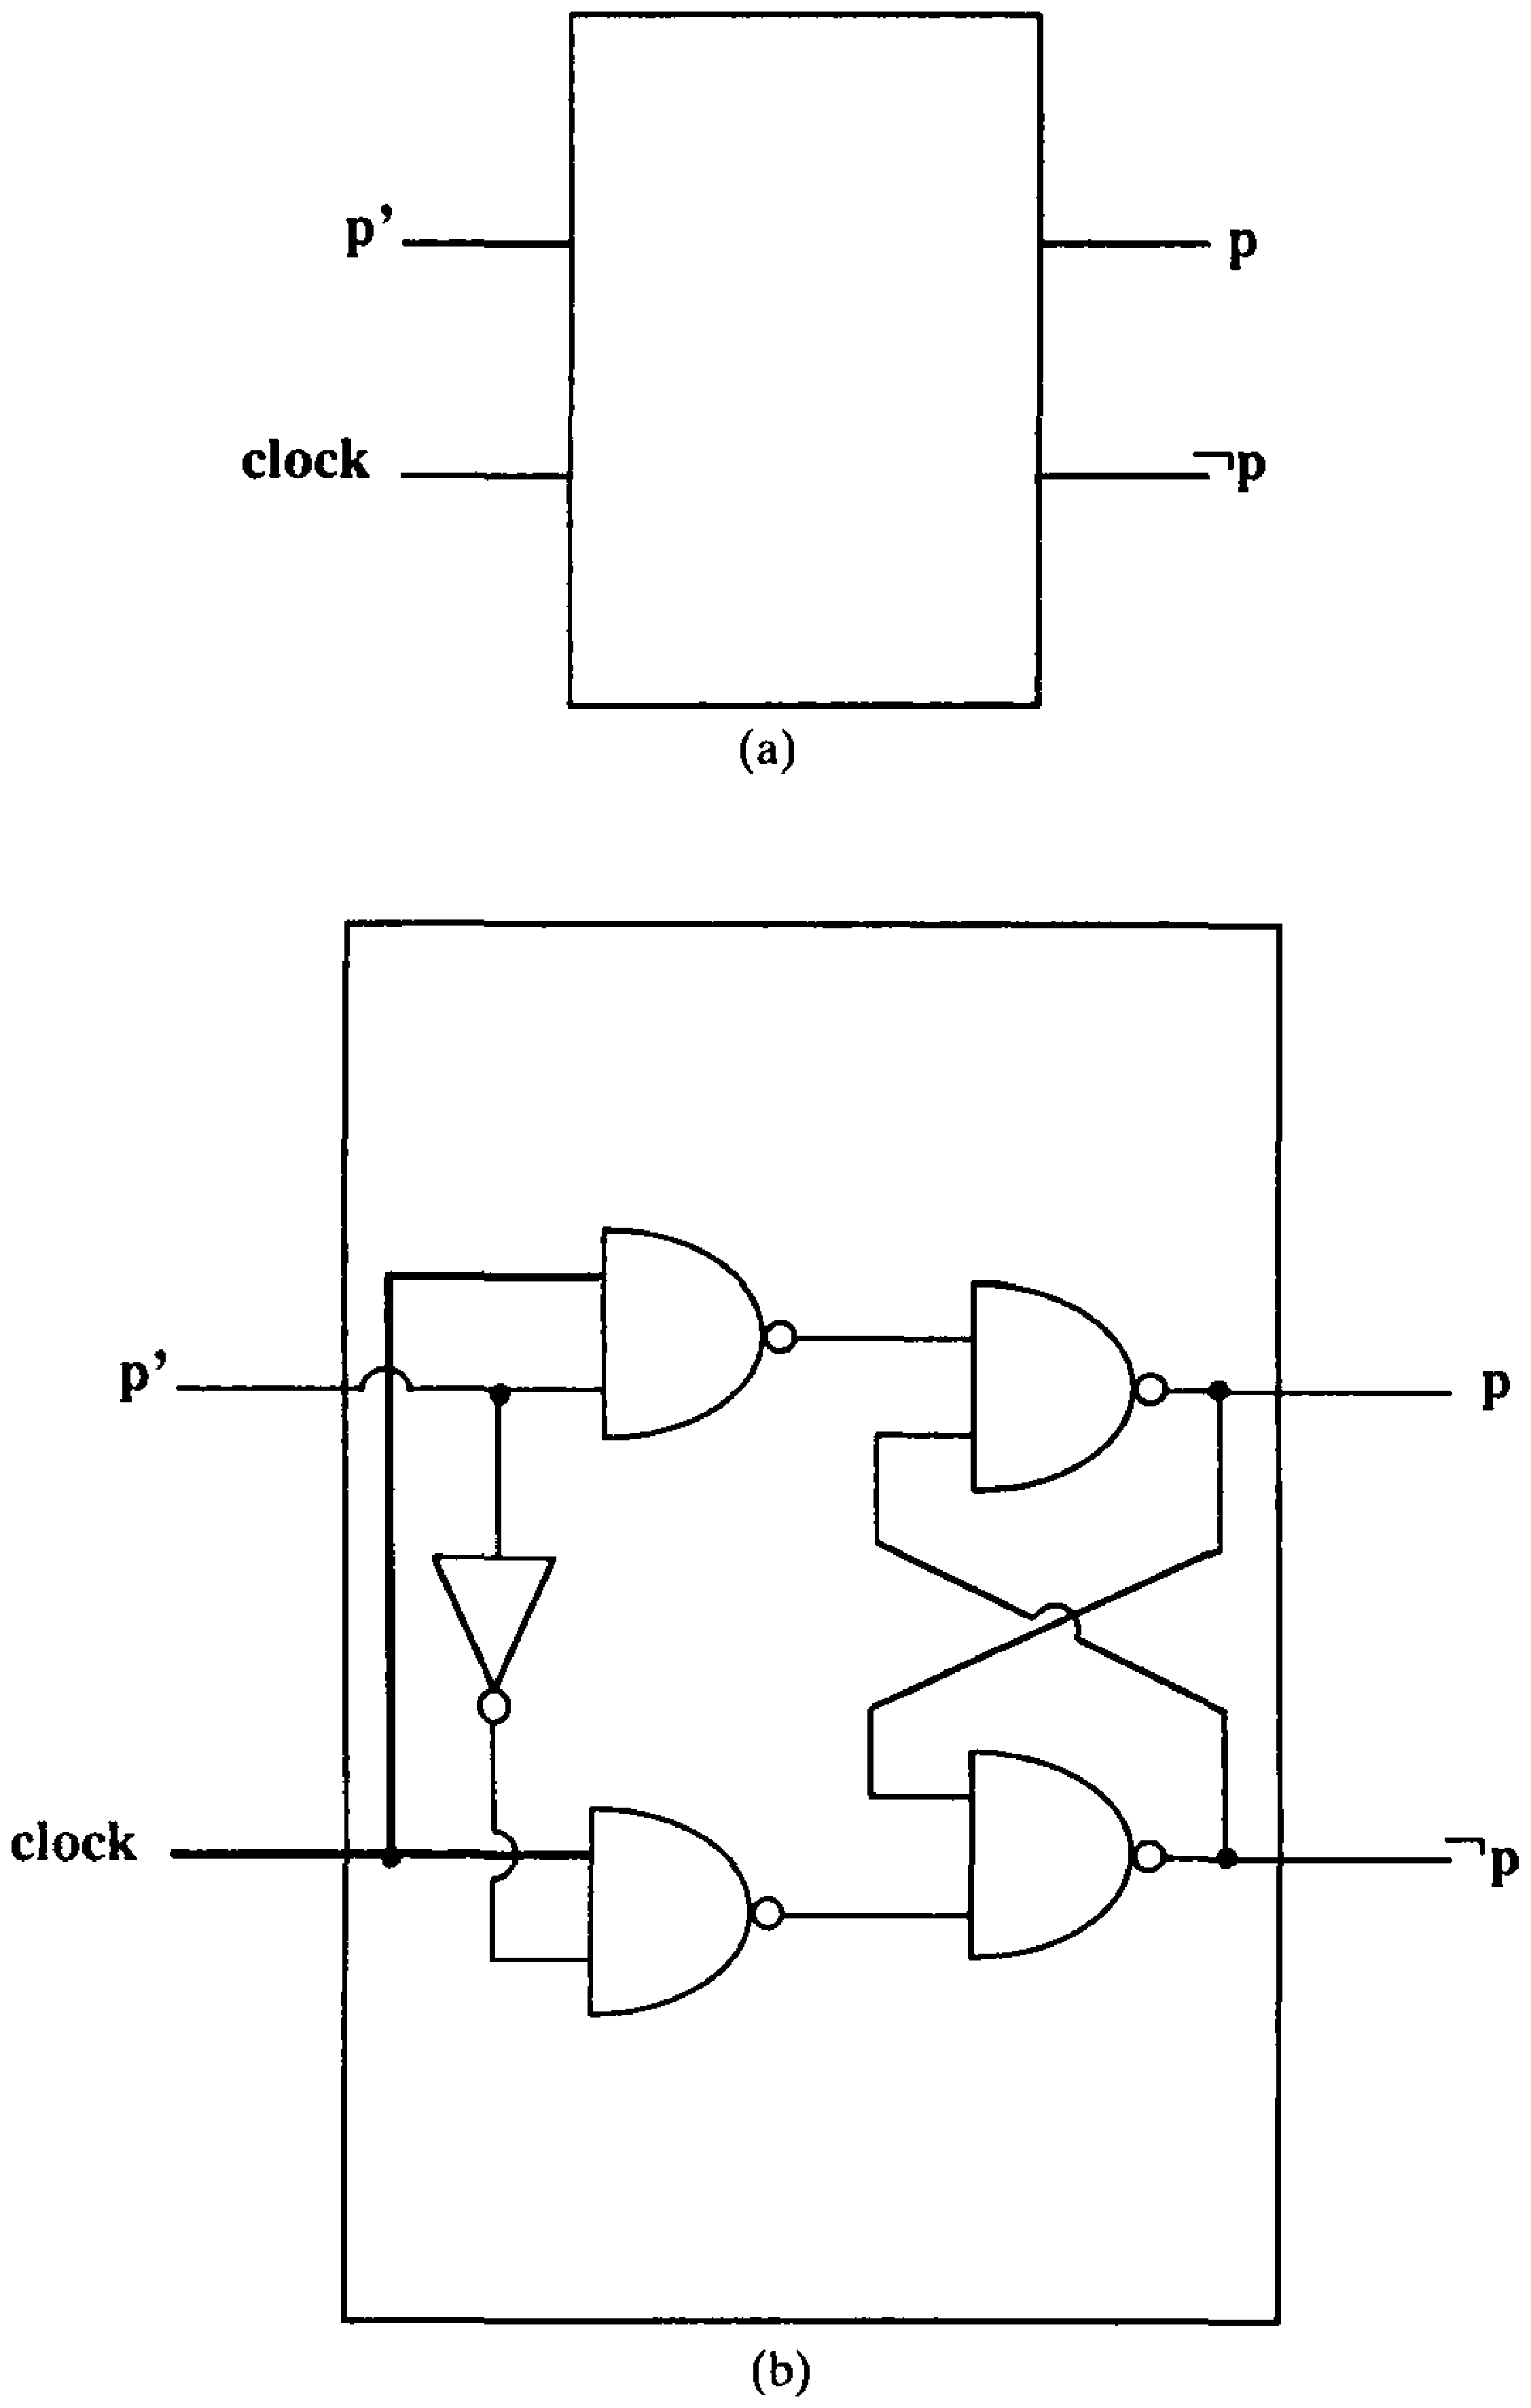
\epsfig{figure=ToFAfigures/fig1-16.eps,width=2.5in}}
\caption{(a) A data flip-flop or latch (b) The circuitry for a D flip-flop}\label{fig-1.16}
\end{figure}

Our alphabets are likely to be far smaller than the ASCII character set, and we
will hence need fewer than 8 bits of information to encode our letters. For
example, if $\Sigma = \{\pmb{b},\pmb{c}\}$, 2 bits, $\pmb{a}_1$ and $\pmb{a}_2$,
will suffice. Our choice of encoding could be $\pmb{00}$ = \<EOS\>, $\pmb{01}=
\pmb{b}$, $\pmb{10}=\pmb{c}$, and $\pmb{11}$ is unused.

In a similar fashion, we must encode state names. A machine with
$S = \{r_0,r_1,r_2,r_3,r_4,r_5\}$ would need 3 bits (denoted by $t_1$, $t_2$,
and $t_3$) to represent the six states. The most natural encoding would be
$r_0 = \pmb{000}$, $r_1 = \pmb{001}$, $r_2 = \pmb{010}$, $r_3 = \pmb{011}$,
$r_4 = \pmb{100}$, and $r_5 = \pmb{101}$, with the combinations $\pmb{110}$ and
$\pmb{111}$ left unused.

Finally, a mechanism for differentiating between final and nonfinal states
must be implemented (although this need not be engaged until the \<EOS\> symbol
is encountered). Recall that we must illuminate the ``acceptance light'' if the
machine terminates in a final state and leave it unlit if the string on the
input tape is instead rejected by the DFA. A second ``rejection light'' can be
added to the physical model, and exactly one of the two will light when \<EOS\>
is scanned by the input head.

% Example 1.12
\subsection*{Example 1.12}

When building a logical circuit from the definition of a DFA, we will find it
convenient to treat \<EOS\> as an input symbol, and define the state transition
function for it by $(\forall s \in S)(\delta(s_1,\<EOS\>) = s)$. Thus, the DFA
in Figure \ref{fig-1.17}a should be thought of as shown in Figure
\ref{fig-1.17}b. As we have only two states, a single state bit will suffice,
representing $s_0$ by $t_1=\pmb{0}$ and $s_1$ by $t_1=\pmb{1}$. Since $\Sigma=
\{\pmb{b},\pmb{c}\}$, we will again use 2 bits, $\pmb{a}_1$ and $\pmb{a}_2$, to
represent the input symbols. As before, $\pmb{00}$ = \<EOS\>, $\pmb{01} = b$,
$\pmb{10} = c$, and $\pmb{11}$ is unused.

% Figure 1.17
\begin{figure}
\centerline{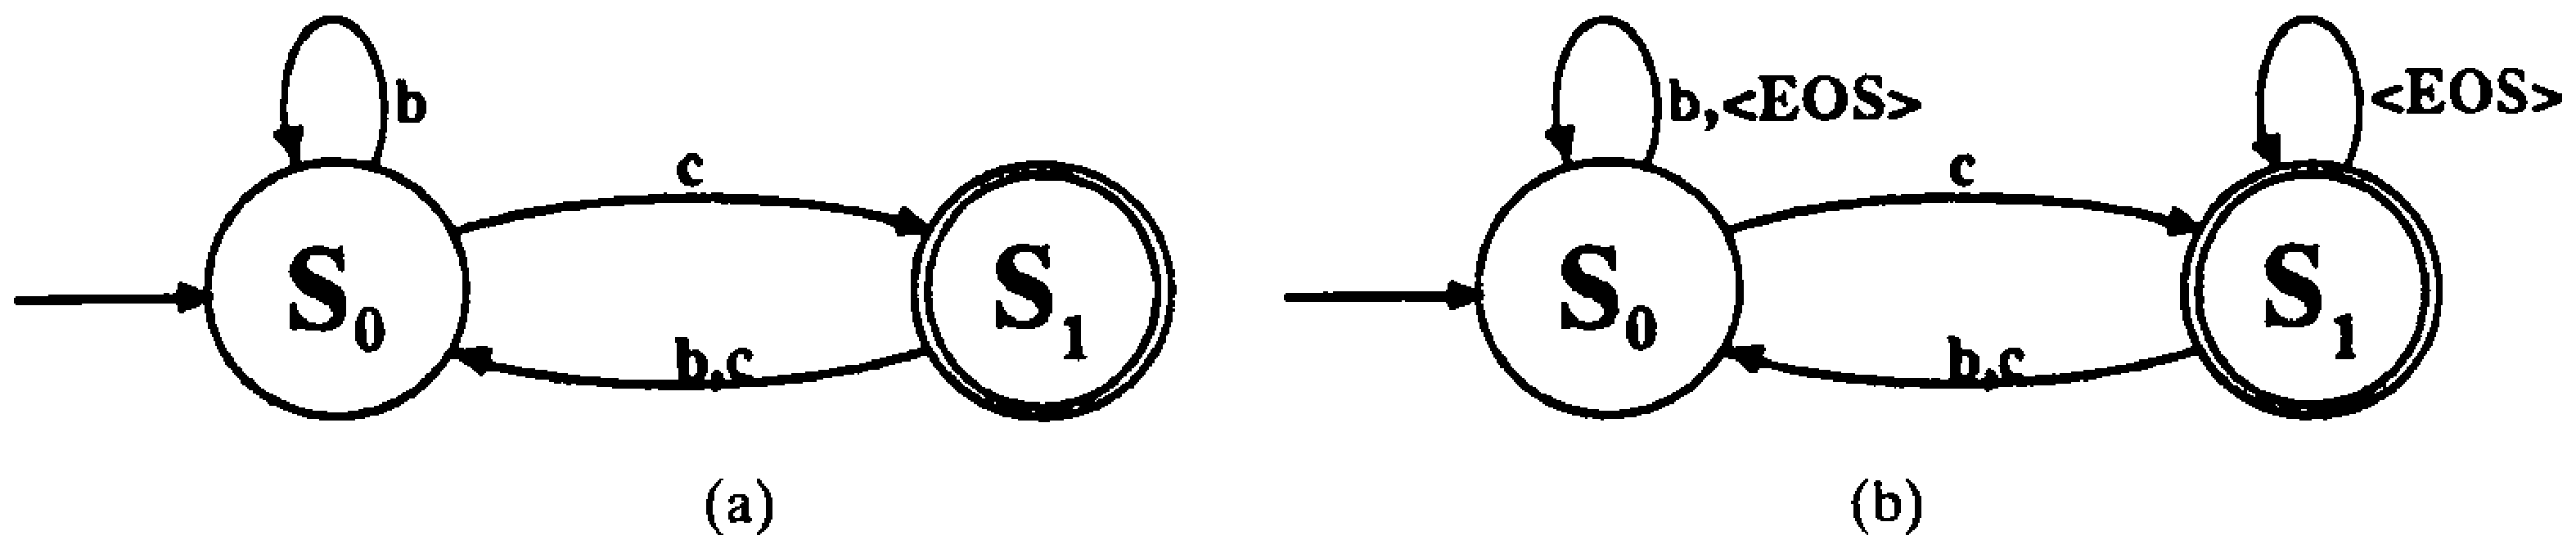
\epsfig{figure=ToFAfigures/fig1-17.eps,width=5in}}
\caption{(a) The DFA discussed in Example 1.12 (b) The expanded state transition
diagram for the DFA implemented in Figure \ref{fig-1.18}}\label{fig-1.17}
\end{figure}

Determining the state transition function will require knowledge of the current
state (represented by the status of $t_1$) and the current input symbol
(represented by the pair of bits $a_1$ and $a_2$). These three input values will
allow the next state $t_1'$ to be calculated. From the $\delta$ function, we
know that
\begin{align*}
\delta(s_0,\pmb{b}) = s_0 \\
\delta(s_0,\pmb{c}) = s_1 \\
\delta(s_1,\pmb{b}) = s_0 \\
\delta(s_1,\pmb{c}) = s_0
\end{align*}
These specifications correspond to the following four rows of the truth table
for $t_1'$:

\begin{center}\begin{tabular}{ccc}
{
\begin{tabular}{ccc|c}
$t_1$ & $\pmb{a}_1$ & $\pmb{a}_2$ & $t_1'$ \\
\hline
$\pmb{0}$ & $\pmb{0}$ & $\pmb{1}$ & $\pmb{0}$ \\
$\pmb{0}$ & $\pmb{1}$ & $\pmb{0}$ & $\pmb{1}$ \\
$\pmb{1}$ & $\pmb{0}$ & $\pmb{1}$ & $\pmb{0}$ \\
$\pmb{1}$ & $\pmb{1}$ & $\pmb{0}$ & $\pmb{0}$
\end{tabular}
} & {
which represents
} & {
\begin{tabular}{cl|c}
$t_1$ & $\pmb{a}_1\ \ \pmb{a}_2$ & $t_1'$ \\
\hline
$s_{\pmb{0}}$ & $\underline{\pmb{0}\ \ \ \ \pmb{1}} = \pmb{b}$ & $s_{\pmb{0}}$ \\
$s_{\pmb{0}}$ & $\underline{\pmb{1}\ \ \ \ \pmb{0}} = \pmb{c}$ & $s_{\pmb{1}}$ \\
$s_{\pmb{1}}$ & $\underline{\pmb{0}\ \ \ \ \pmb{1}} = \pmb{b}$ & $s_{\pmb{0}}$ \\
$s_{\pmb{1}}$ & $\underline{\pmb{1}\ \ \ \ \pmb{0}} = \pmb{c}$ & $s_{\pmb{0}}$
\end{tabular}
}
\end{tabular}\end{center}

Adding the state transitions for \<EOS\> and using * to represent the
outcome for the two rows corresponding to the unused combination $\pmb{a}_1
\pmb{a}_2=\pmb{11}$ fills out the eight rows of the complete truth table, as
shown in Table \ref{tbl-1.2}.

% Table 1.2
\begin{table}[h]\caption{}\label{tbl-1.2}
\begin{center}
\begin{tabular}{ccc|c}
$t_1$ & $\pmb{a}_1$ & $\pmb{a}_2$ & $t_1'$ \\
\hline
$\pmb{0}$ & $\pmb{0}$ & $\pmb{0}$ & $\pmb{0}$ \\
$\pmb{0}$ & $\pmb{0}$ & $\pmb{1}$ & $\pmb{0}$ \\
$\pmb{0}$ & $\pmb{1}$ & $\pmb{0}$ & $\pmb{1}$ \\
$\pmb{0}$ & $\pmb{1}$ & $\pmb{1}$ & * \\
$\pmb{1}$ & $\pmb{0}$ & $\pmb{0}$ & $\pmb{1}$ \\
$\pmb{1}$ & $\pmb{0}$ & $\pmb{1}$ & $\pmb{0}$ \\
$\pmb{1}$ & $\pmb{1}$ & $\pmb{0}$ & $\pmb{0}$ \\
$\pmb{1}$ & $\pmb{1}$ & $\pmb{1}$ & *
\end{tabular}
\end{center}
\end{table}

If we arbitrarily assume that the two don't-care combinations (*) are zero, the
principle disjunctive normal form of $t_1'$ contains just two terms:
$(\neg t_1\wedge\pmb{a}_1\wedge\neg\pmb{a}_2)\vee(t_1\wedge\neg\pmb{a}_1\wedge
\neg\pmb{a}_2)$. It is profitable to reassign the don't-care value in the fourth
row to $\pmb{1}$, since the expression can then be shortened to $(\neg t_1\wedge
\pmb{a}_1)\vee(t_1\wedge\neg\pmb{a}_1\wedge\neg\pmb{a}_2)$ by applying standard
techniques for minimizing Boolean functions. Incorporating this into a feedback
loop with a D flip-flop provides the heart of the digital logic circuit
representing the DFA, as shown in Figure \ref{fig-1.18}.

% Figure 1.18
\begin{figure}
\centerline{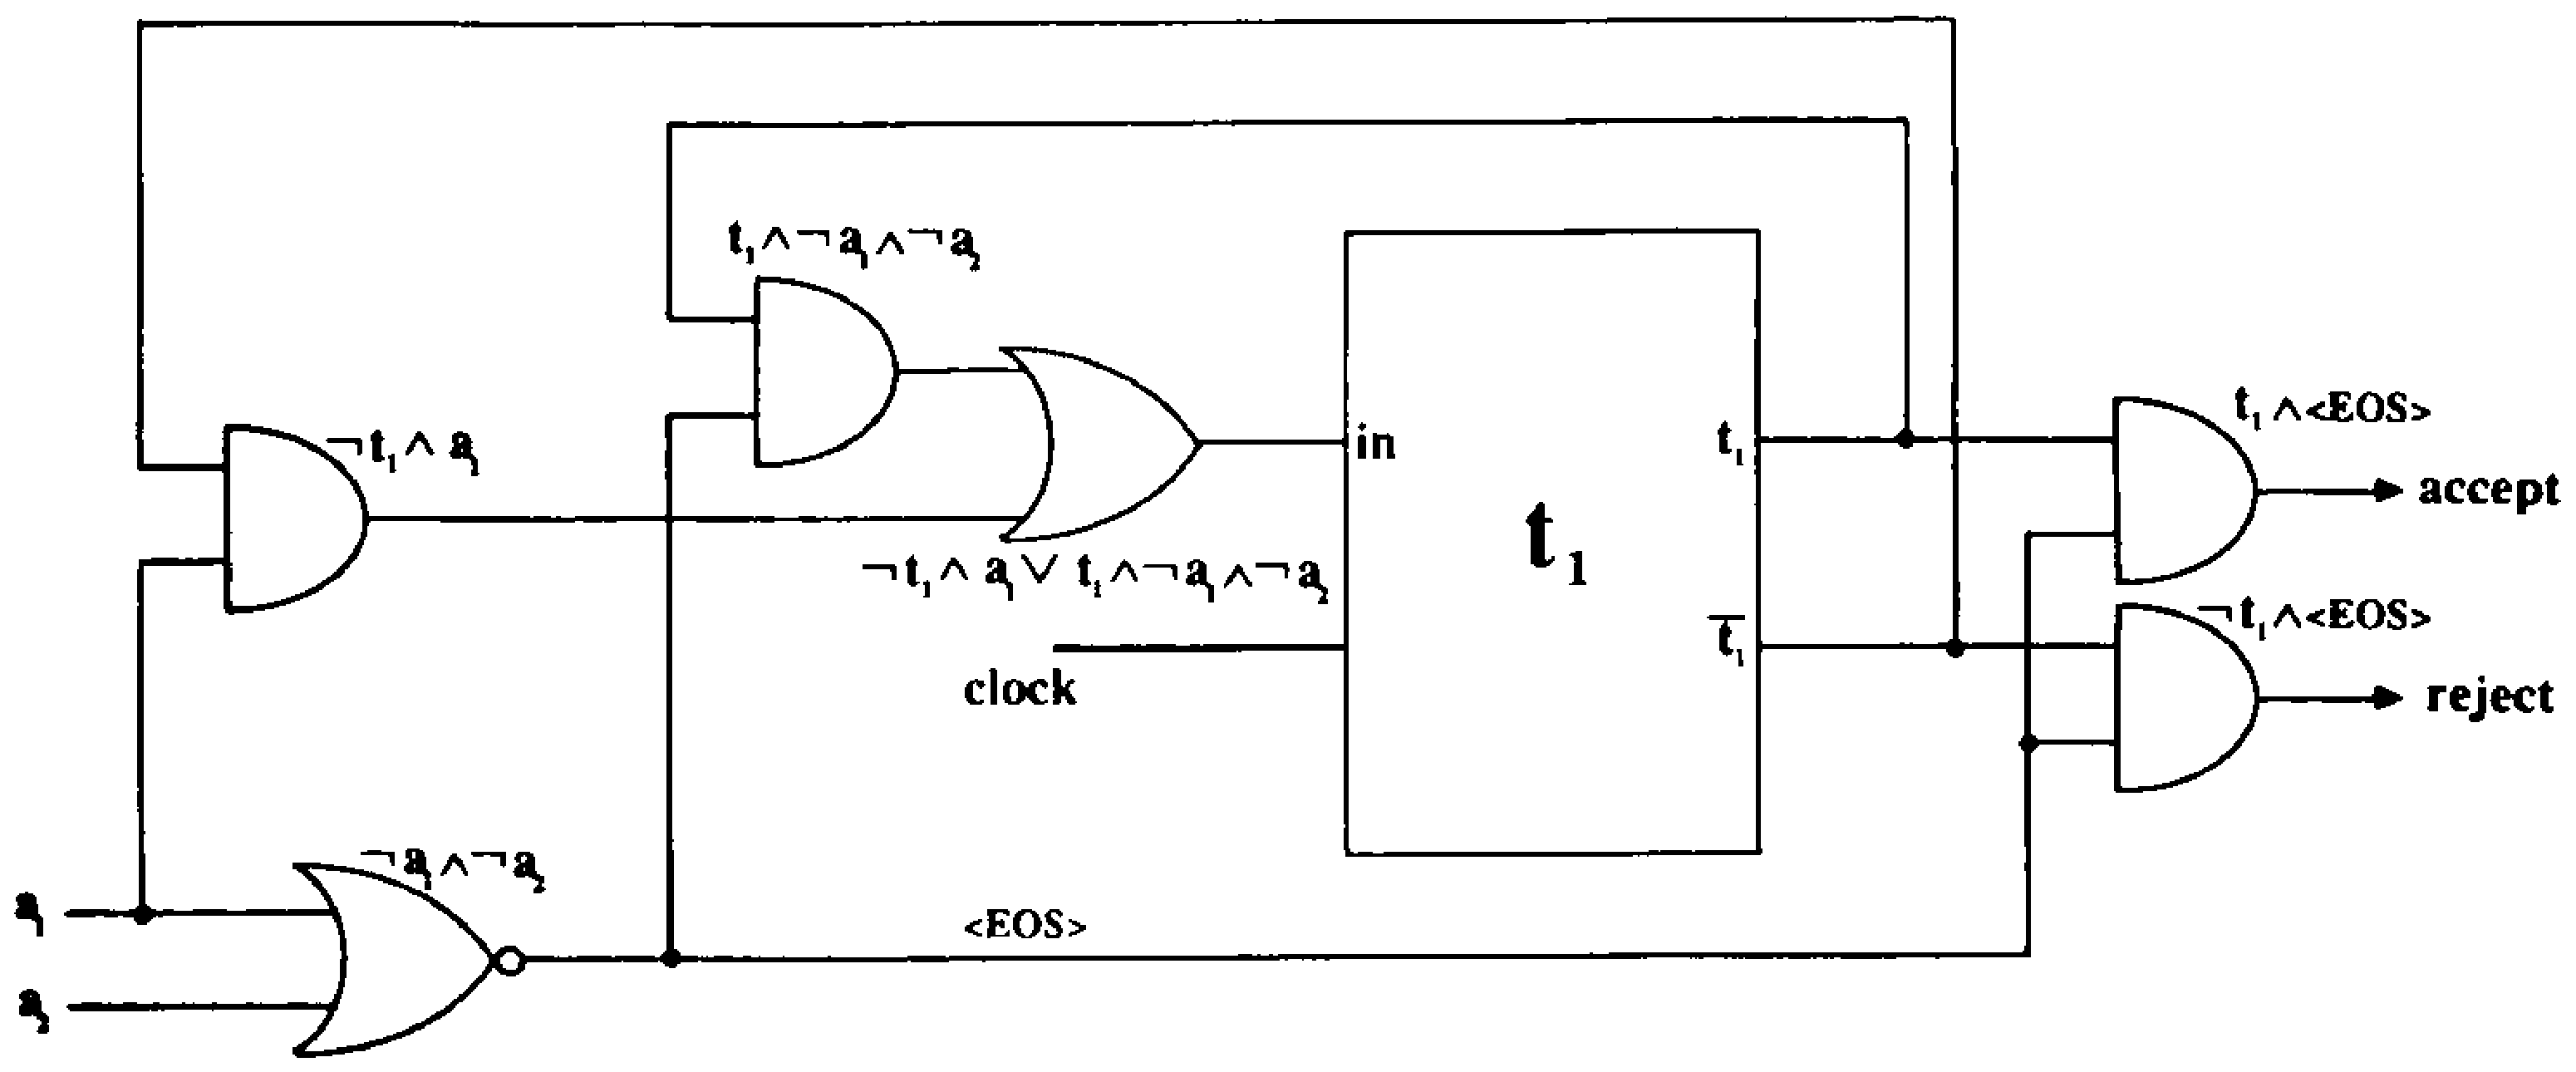
\epsfig{figure=ToFAfigures/fig1-18.eps,width=6in}}
\caption{The circuitry implementing the DFA discussed in Example 1.12}\label{fig-1.18}
\end{figure}

The accept portion of the circuitry\index{accept circuitry} ensures that we do not indicate acceptance
when passing through the final state; it is only activated when we are in a
final state while scanning the \<EOS\> symbol. Similarly, the reject circuitry
can only be activated when the \<EOS\> symbol is encountered. When there are
several final states, this part of the circuitry becomes correspondingly more
complex. It is instructive to follow the effect a string such as $\pmb{bcc}$ has
on the above circuit. Define $\pmb{a}_i(j)$ as the $j$th value the bit $\pmb{a}_i$
takes on as the string $\pmb{bcc}$ is processed; that is, $\pmb{a}_i(j)$ is the
value of $\pmb{a}_i$ during the $j$th clock pulse. We then have
\begin{center}\begin{tabular}{r@{ $=$ }l@{$\qquad$}r@{ $=$ }l@{$\qquad\Rightarrow$ }l}
$\pmb{a}_1(1)$ & $\pmb{0}$ & $\pmb{a}_2(1)$ & $\pmb{1}$ & $\pmb{b}$ \\
$\pmb{a}_1(2)$ & $\pmb{1}$ & $\pmb{a}_2(2)$ & $\pmb{0}$ & $\pmb{c}$ \\
$\pmb{a}_1(3)$ & $\pmb{1}$ & $\pmb{a}_2(3)$ & $\pmb{0}$ & $\pmb{c}$ \\
$\pmb{a}_1(4)$ & $\pmb{0}$ & $\pmb{a}_2(4)$ & $\pmb{0}$ & \<EOS\>
\end{tabular}\end{center}
Trace the circuit through four clock pulses (starting with $t_1=\pmb{0}$), and
observe the current values that $t_1$ assumes, noting that it corresponds to the
appropriate state of the machine as each input symbol is scanned.

Note that a six-state machine would require more and substantially larger
truth tables. Since a state encoding would now need to specify $t_1$, $t_2$, and
$t_3$, three different truth tables (for $t_1'$, $t_2'$, and $t_3'$) must be
constructed to predict the next state transition. More significantly, the input
variables would include $t_1$, $t_2$, $t_3$, $\pmb{a}_1$, and $\pmb{a}_2$,
making each table 32 rows long. Three D flip-flop feedback loops would be
necessary to store the three values $t_1$, $t_2$, and $t_3$.

Also, physical logic circuits of this type have the disconcerting habit of
initializing to some random configuration the first time power is applied to the
network. A true working model would thus need a \emph{reset}\index{reset circuitry} circuit to
initialize each $t_i$ to $\pmb{0}$ in order to ensure that the machine started
in state $s_0$. Slightly more complex set-reset flip-flops can be used to
provide a hardware solution to this problem. However, a simple algorithmic
solution would require the input tape to have a \emph{leading} start-of-string
symbol \<SOS\>. The definition of the state transition function should be
expanded so that scanning the \<SOS\> symbol from any state will automatically
transfer control to $s_0$. We will adopt the convention that \<SOS\> will be
represented by the highest binary code; in ASCII, for example, this would be
$\pmb{11111111}$, while in the preceding example it would be $\pmb{11}$. To
promote uniformity in the exercises, it is suggested that \<SOS\> should always
be given the highest binary code and \<EOS\> be represented by binary zero; as
in the examples given here, the symbols in $\Sigma$ should be numbered
sequentially according to their natural alphabetical order. In a similar
fashion, numbered states should be given their corresponding binary codes. The
reader should note, however, that other encodings might result in less complex
circuitry.

\subsection*{Example 1.13}

As a more complex example of automaton circuitry, consider the DFA displayed in
Figure \ref{fig-1.19}. Two flip-flops $t_1$ and $t_2$ will be necessary to
represent the three states, most naturally encoded as $s_0 = \pmb{00}$, $s_1 =
\pmb{01}$, $s_2 = \pmb{10}$, with $s_3 = \pmb{11}$ unused. Employing both
\<SOS\> and \<EOS\> encodings yields the DFA in Figure \ref{fig-1.20}.

% Figure 1.19
\begin{figure}
\centerline{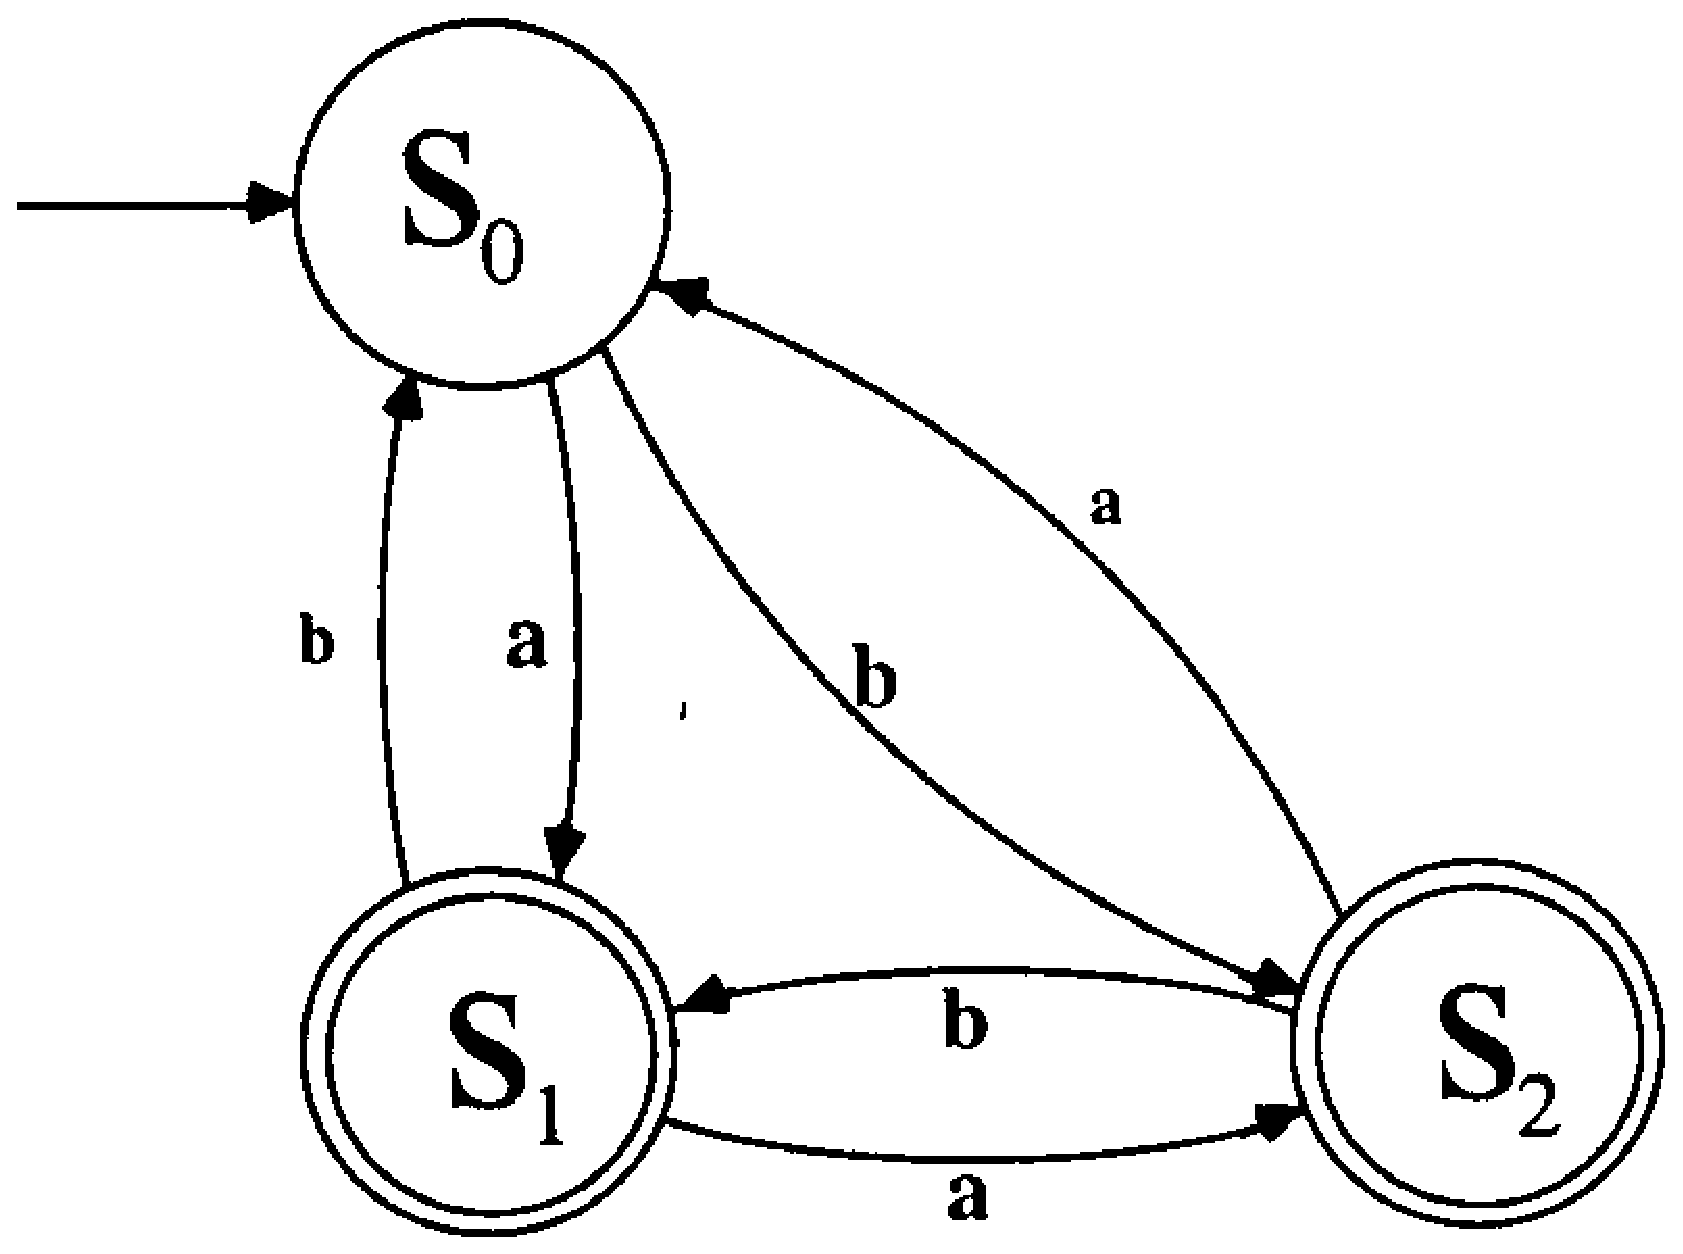
\epsfig{figure=ToFAfigures/fig1-19.eps,width=3in}}
\caption{The DFA discussed in Example 1.13}\label{fig-1.19}
\end{figure}

Note that we must account for the possibility that the circuitry might be
randomly initialized to $t_1=\pmb{1}$ and $t_2=\pmb{1}$; we must ensure that
scanning the \<SOS\> symbol moves us back into the ``real'' part of the machine.
Two bits of information ($\pmb{a}_1$ and $\pmb{a}_2$) are also needed to
describe the input symbols. Following our conventions, we assign \<EOS\> $=
\pmb{00}$, $\pmb{a} = \pmb{01}$, $\pmb{b} = \pmb{10}$, and \<SOS\> $= \pmb{11}$.
The truth table for both the transition function and the conditions for
acceptance is given in Table \ref{tbl-1.3}.

In the first row, $t_1=\pmb{0}$ and $t_2=\pmb{0}$ indicate state $s_0$, while
$\pmb{a}_1=\pmb{0}$ and $\pmb{a}_2=\pmb{0}$ denote the \<EOS\> symbol. Since $\delta(
s_0,\<EOS\>) = s_0$, $t_1'=\pmb{0}$ and $t_2'=\pmb{0}$. We do not want to accept
a string that ends in $s_0$, so {\bf accept}$ = 0$ also. The remaining rows are
determined similarly. The (nonminimized) circuitry for this DFA is shown in
Figure \ref{fig-1.21}.

% Table 1.3
\begin{table}\caption{}\label{tbl-1.3}
\begin{center}
\begin{tabular}{cccc|ccc}
$t_1$ & $t_2$ & $\pmb{a}_1$ & $\pmb{a}_2$ & $t_1'$ & $t_2'$ & {\bf accept} \\
\hline
$\pmb{0}$ & $\pmb{0}$ & $\pmb{0}$ & $\pmb{0}$ & $\pmb{0}$ & $\pmb{0}$ & $\pmb{0}$ \\
$\pmb{0}$ & $\pmb{0}$ & $\pmb{0}$ & $\pmb{1}$ & $\pmb{0}$ & $\pmb{1}$ & $\pmb{0}$ \\
$\pmb{0}$ & $\pmb{0}$ & $\pmb{1}$ & $\pmb{0}$ & $\pmb{1}$ & $\pmb{0}$ & $\pmb{0}$ \\
$\pmb{0}$ & $\pmb{0}$ & $\pmb{1}$ & $\pmb{1}$ & $\pmb{0}$ & $\pmb{0}$ & $\pmb{0}$ \\
$\pmb{0}$ & $\pmb{1}$ & $\pmb{0}$ & $\pmb{0}$ & $\pmb{0}$ & $\pmb{1}$ & $\pmb{1}$ \\
$\pmb{0}$ & $\pmb{1}$ & $\pmb{0}$ & $\pmb{1}$ & $\pmb{1}$ & $\pmb{0}$ & $\pmb{0}$ \\
$\pmb{0}$ & $\pmb{1}$ & $\pmb{1}$ & $\pmb{0}$ & $\pmb{0}$ & $\pmb{0}$ & $\pmb{0}$ \\
$\pmb{0}$ & $\pmb{1}$ & $\pmb{1}$ & $\pmb{1}$ & $\pmb{0}$ & $\pmb{0}$ & $\pmb{0}$ \\
$\pmb{1}$ & $\pmb{0}$ & $\pmb{0}$ & $\pmb{0}$ & $\pmb{1}$ & $\pmb{0}$ & $\pmb{1}$ \\
$\pmb{1}$ & $\pmb{0}$ & $\pmb{0}$ & $\pmb{1}$ & $\pmb{0}$ & $\pmb{0}$ & $\pmb{0}$ \\
$\pmb{1}$ & $\pmb{0}$ & $\pmb{1}$ & $\pmb{0}$ & $\pmb{0}$ & $\pmb{1}$ & $\pmb{0}$ \\
$\pmb{1}$ & $\pmb{0}$ & $\pmb{1}$ & $\pmb{1}$ & $\pmb{0}$ & $\pmb{0}$ & $\pmb{0}$ \\
$\pmb{1}$ & $\pmb{1}$ & $\pmb{0}$ & $\pmb{0}$ & * & * & * \\
$\pmb{1}$ & $\pmb{1}$ & $\pmb{0}$ & $\pmb{1}$ & * & * & * \\
$\pmb{1}$ & $\pmb{1}$ & $\pmb{1}$ & $\pmb{0}$ & * & * & * \\
$\pmb{1}$ & $\pmb{1}$ & $\pmb{1}$ & $\pmb{1}$ & $\pmb{0}$ & $\pmb{0}$ & $\pmb{0}$
\end{tabular}
\end{center}
\end{table}
\

% Figure 1.20
\begin{figure}
\centerline{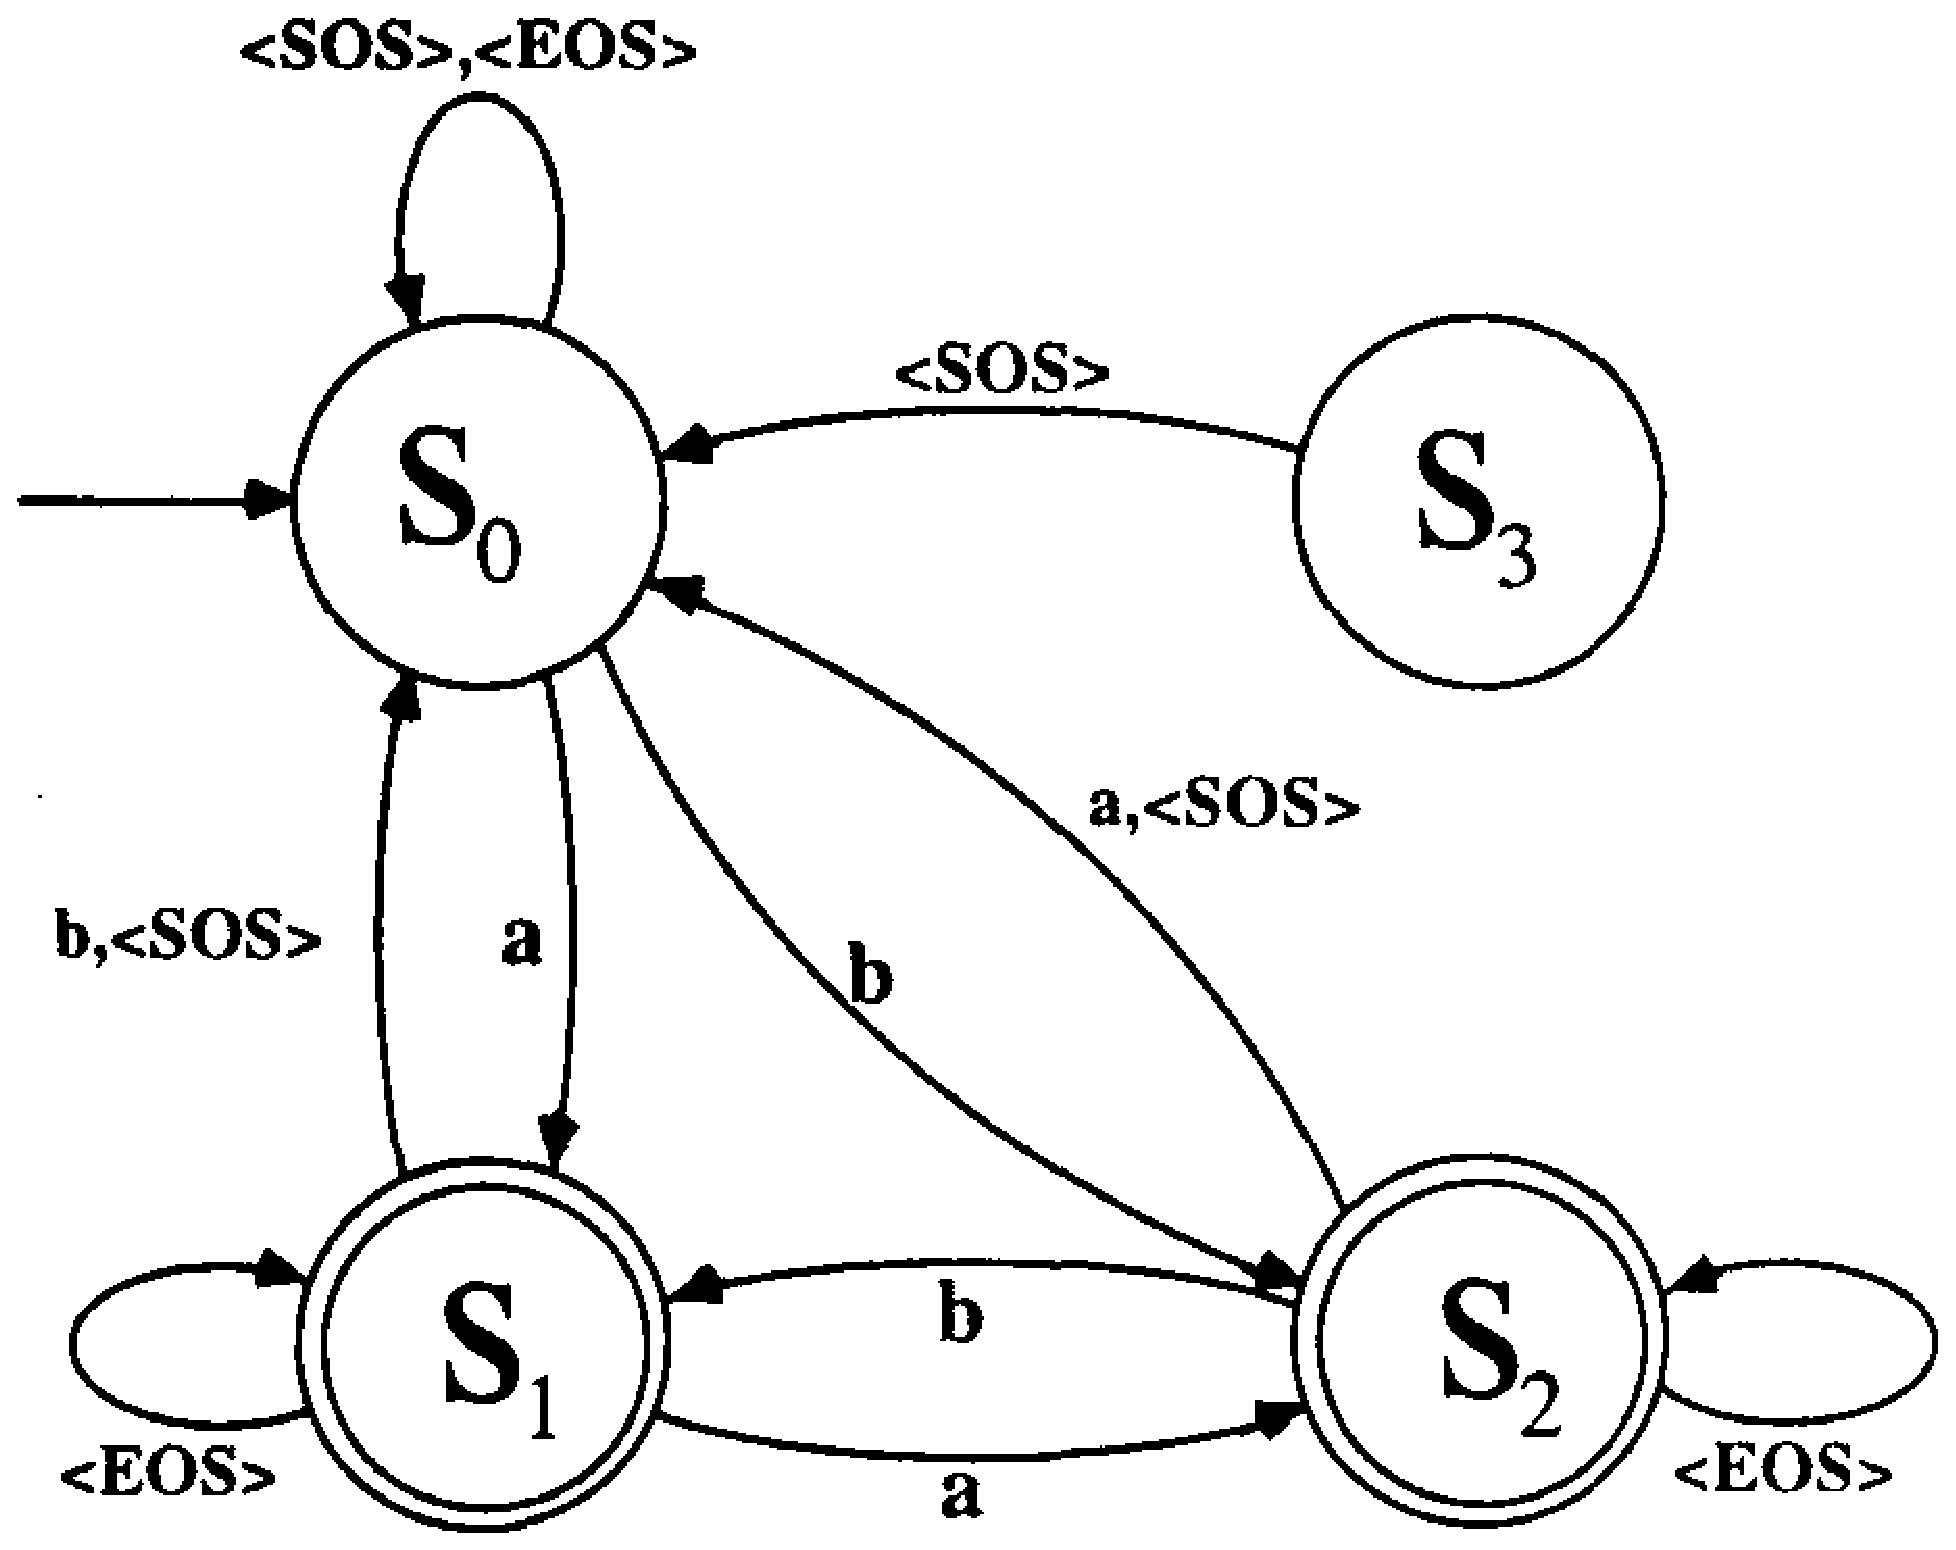
\epsfig{figure=ToFAfigures/fig1-20.eps,width=3.5in}}
\caption{The expanded state transition diagram for the DFA implemented in Figure
\ref{fig-1.21}}\label{fig-1.20}
\end{figure}

% Figure 1.21
\begin{figure}
\centerline{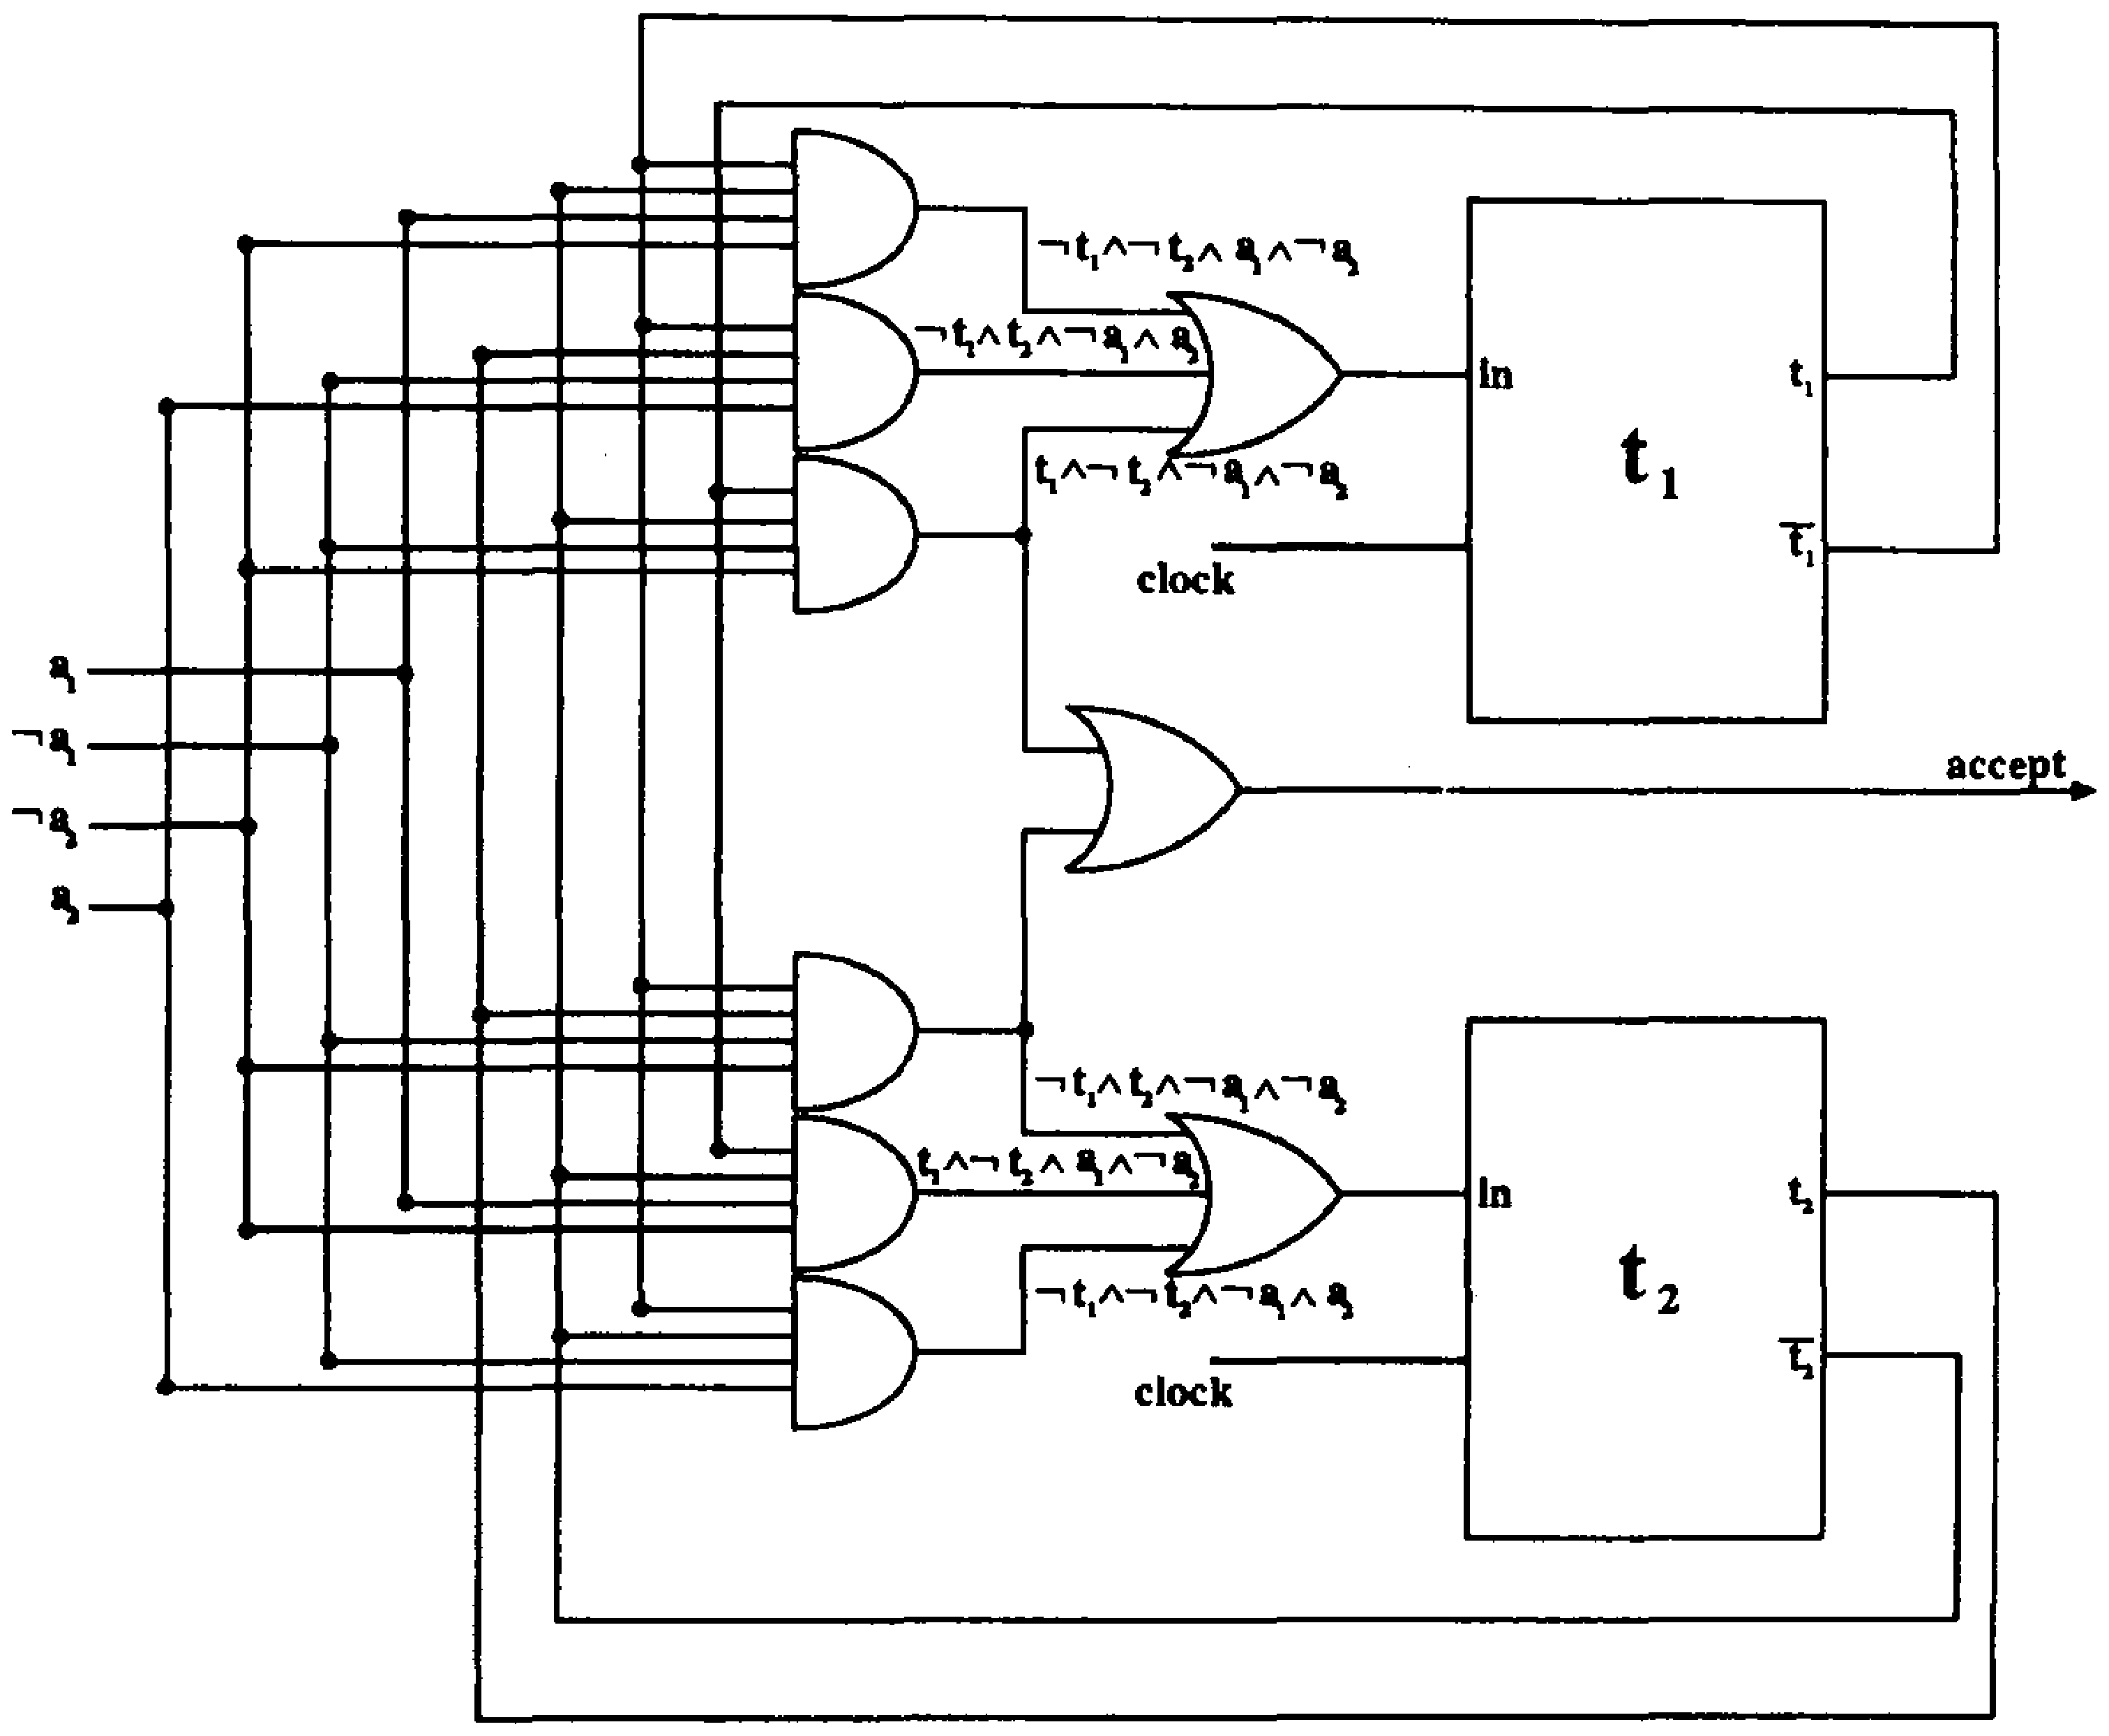
\epsfig{figure=ToFAfigures/fig1-21.eps,height=3.8in}}
\caption{The circuitry implementing the DFA discussed in Example 1.13}\label{fig-1.21}
\end{figure}

\section{Applications of Finite Automata}\label{sec-1.5}

In this chapter we have described the simplest form of finite automaton, the
DFA. Other forms of automata, such as nondeterministic finite automata, pushdown
automata, and Turing machines, are introduced later in the text. We close this 
chapter with three examples to motivate the material in the succeeding chapters.

When presenting automata in this chapter, we made no effort to construct the
\Index{minimal machine}.  A \emph{minimal} machine for a given language is one
that has the least number of states required to accept that language.

\subsection*{Example 1.14}

In Example 1.5, the vending machine kept track of the amount of change
that had been deposited up to $50$\cent. Since the candy bars cost only
30\cent, there is no need to count up to $50$\cent. In this sense, the machine
is not optimal, since a less complex machine can perform the same task, as shown
in Figure \ref{fig-1.22}. The corresponding quintuple is $\langle\{\pmb{n},
\pmb{d},\pmb{q}\},\{s_0,s_5,s_{10},s_{15},s_{20},s_{25},s_{30}\},s_0,\delta,
\{s_{30}\}\rangle$, where for each state $s_i$, $\delta$ is defined by
\begin{align*}
\delta(s_i,\pmb{n}) = s_{min\{30,i+5)\}} \\
\delta(s_i,\pmb{d}) = s_{min\{30,i+10\}} \\
\delta(s_i,\pmb{q}) = s_{min\{30,i+25\}}
\end{align*}

Note that the higher-numbered states in Example 1.5 were all
effectively ``remembering'' the same thing, that enough coins had been deposited.
These final states have been coalesced into a single final state to produce the
more efficient machine in Figure \ref{fig-1.22}. In the next two chapters, we
develop the theoretical background and algorithms necessary to construct from
an arbitrary DFA the minimal machine that accepts the same language.

As another illustration of the utility of concepts relating to finite-state
machines, we will consider the formalism used by many text editors to search for
a particular target string pattern in a text file. To find $\pmb{ababb}$ in a
file, for example, a naive approach might consist of checking whether the first
five characters of the file fit this pattern, and next checking characters 2
through 6 to find a match, and so on. This results in examining file characters
more than once; it ought to be possible to remember past values, and avoid such
duplication. Consider the text string $\pmb{aabababbb}$. By the time the fifth
character is scanned, we have matched the first four characters of $\pmb{ababb}$.
Unfortunately, $\pmb{a}$, the sixth character of $\pmb{aabababbb}$, does not produce
the final match; however, since characters 4,5, and 6 ($\pmb{aba}$) now match the
first three characters of the target string, it does allow for the possibility
of characters 4 through 8 matching (as is indeed the case in this example). This
leads to a general rule: If we have matched the first four letters of the target
string, and the next character happens to be $\pmb{a}$ (rather than the desired
$\pmb{b}$), we must remember that we have now matched the first three letters of
the target string.

% Figure 1.22
\begin{figure}
\centerline{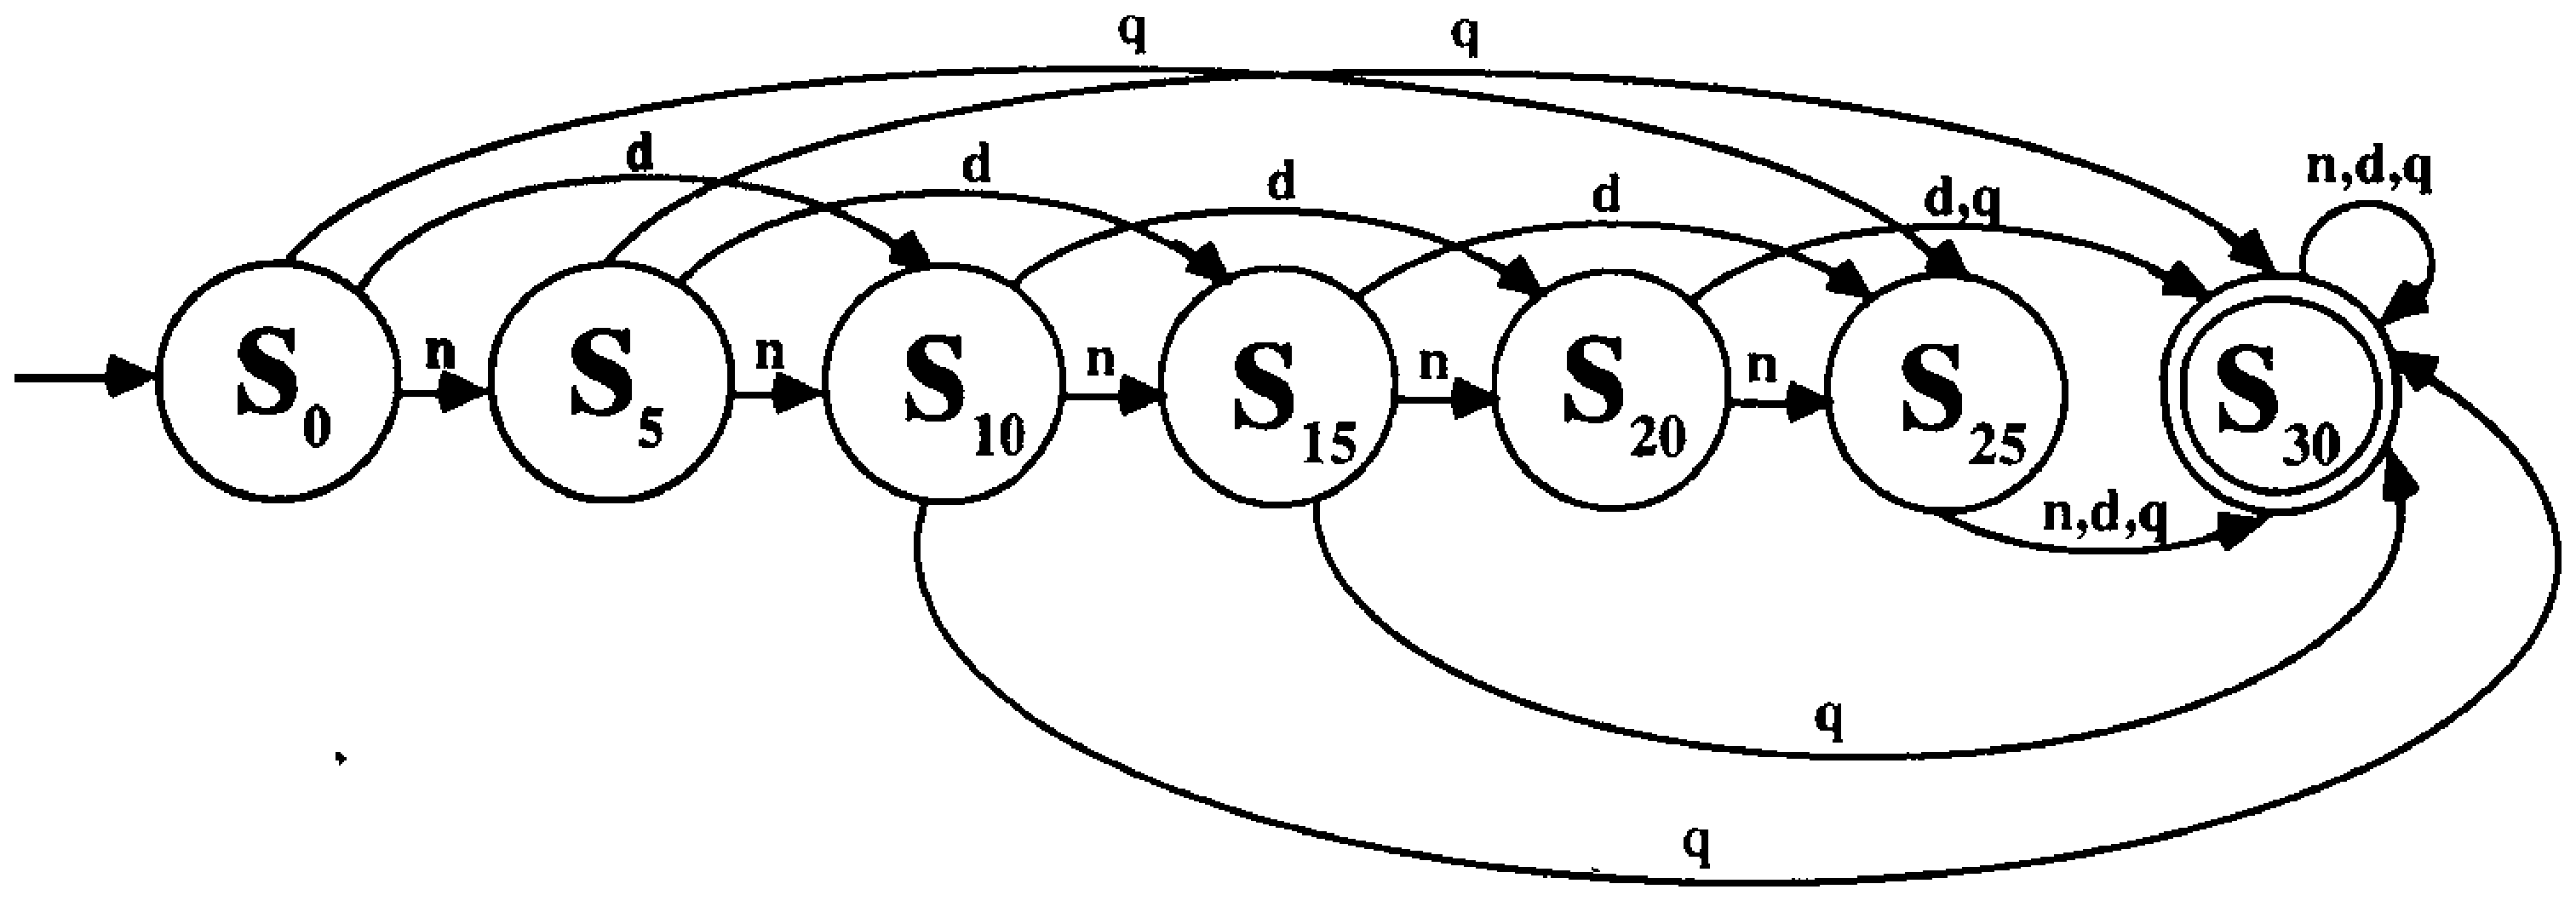
\epsfig{figure=ToFAfigures/fig1-22.eps,width=5.5in}}
\caption{The automaton discussed in Example 1.14}\label{fig-1.22}
\end{figure}

``Rules'' such as these are actually the state transitions in the DFA given in
the next example. State $s_i$ represents having matched the first $i$ characters
of the target string, and the rule developed above is succinctly stated as
$\delta(s_4,\pmb{a})=s_3$.

\subsection*{Example 1.15}

A DFA that accepts all strings that contain $\pmb{ababb}$ as a substring is
displayed in Figure \ref{fig-1.23}. The corresponding quintuple is
\[ \langle\{\pmb{a},\pmb{b}\},\{s_0,s_1,s_2,s_3,s_4,s_5\},s_0,\delta,\{s_5\}
	\rangle, \]
where $\delta$ is defined by
\begin{center}\begin{tabular}{c|cc}
$\delta$ & $\pmb{a}$ & $\pmb{b}$ \\
\hline
$s_0$ & $s_1$ & $s_0$ \\
$s_1$ & $s_1$ & $s_2$ \\
$s_2$ & $s_3$ & $s_0$ \\
$s_3$ & $s_1$ & $s_4$ \\
$s_4$ & $s_3$ & $s_5$ \\
$s_5$ & $s_5$ & $s_5$
\end{tabular}\end{center}

% Figure 1.23
\begin{figure}
\centerline{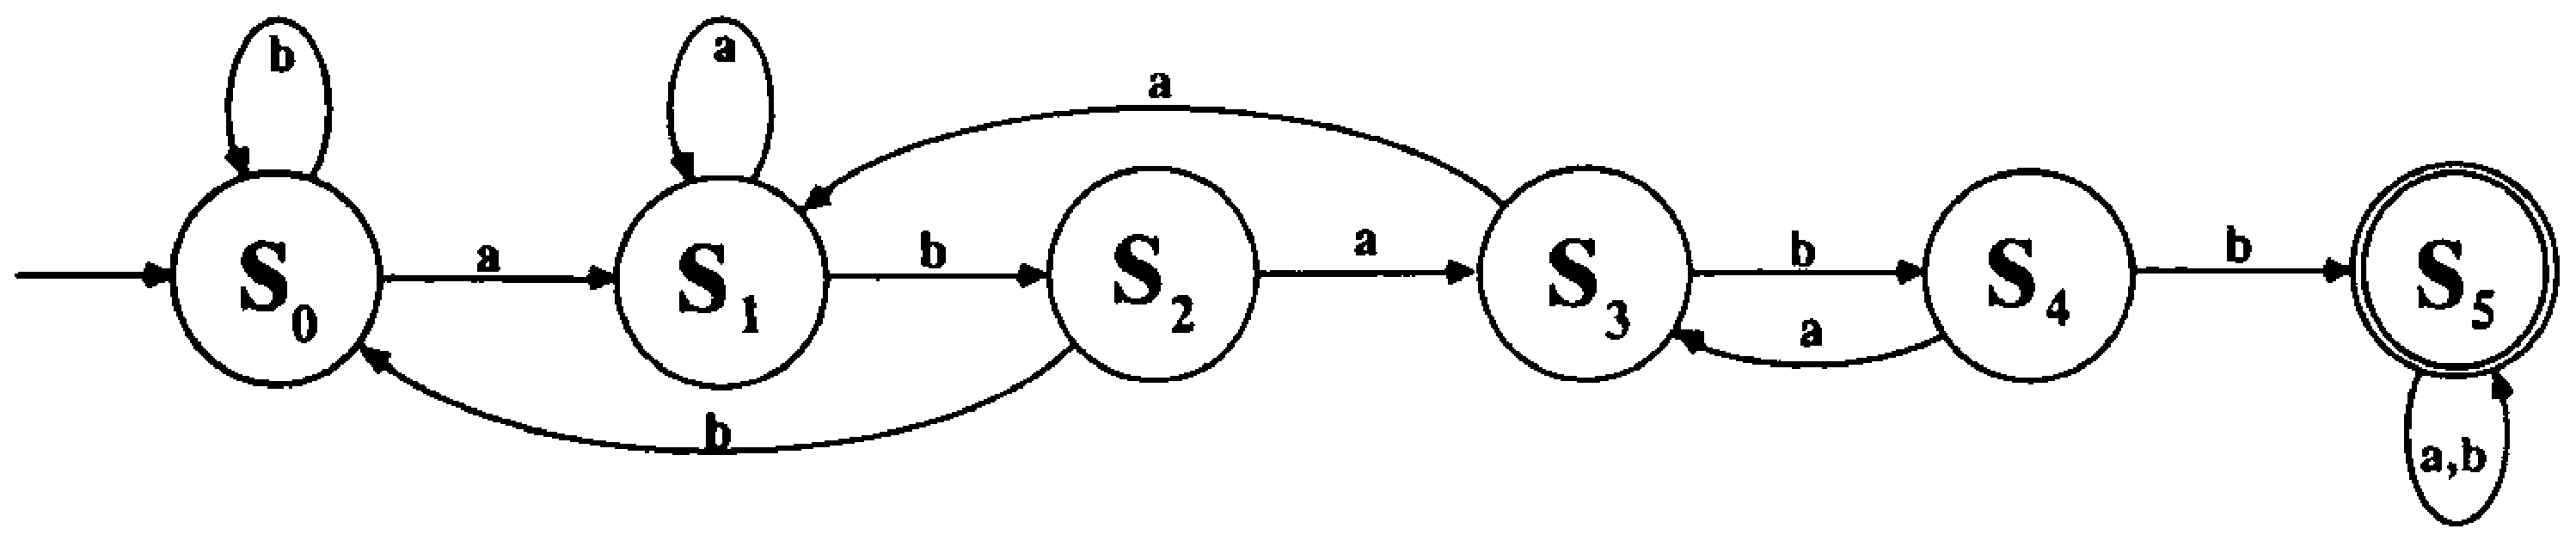
\epsfig{figure=ToFAfigures/fig1-23.eps,width=6.5in}}
\caption{A DFA that accepts strings containing $\pmb{ababb}$}\label{fig-1.23}
\end{figure}

It is a worthwhile exercise to test the operation of this DFA on several text
strings and verify that the automaton is indeed in state $s_i$ exactly when it
has matched the first $i$ characters of the target string. Note that if we did
not care what the third character of the substring was (that is, if we were
searching for occurrences of $\pmb{ababb}$ or $\pmb{abbbb}$), a trivial modification
of the above machine would allow us to search for both substrings at once, as
shown in Figure \ref{fig-1.24}. The corresponding quintuple is
$\langle\{\pmb{a},\pmb{b}\},\{s_0,s_1,s_2,s_3,s_4,s_5\},s_0,\delta,\{s_5\}\rangle$, where
$\delta$ is defined by
\begin{center}\begin{tabular}{c|cc}
$\delta$ & $\pmb{a}$ & $\pmb{b}$ \\
\hline
$s_0$ & $s_1$ & $s_0$ \\
$s_1$ & $s_1$ & $s_2$ \\
$s_2$ & $s_3$ & $s_3$ \\
$s_3$ & $s_1$ & $s_4$ \\
$s_4$ & $s_3$ & $s_5$ \\
$s_5$ & $s_5$ & $s_5$
\end{tabular}\end{center}

% Figure 1.24
\begin{figure}[h]
\centerline{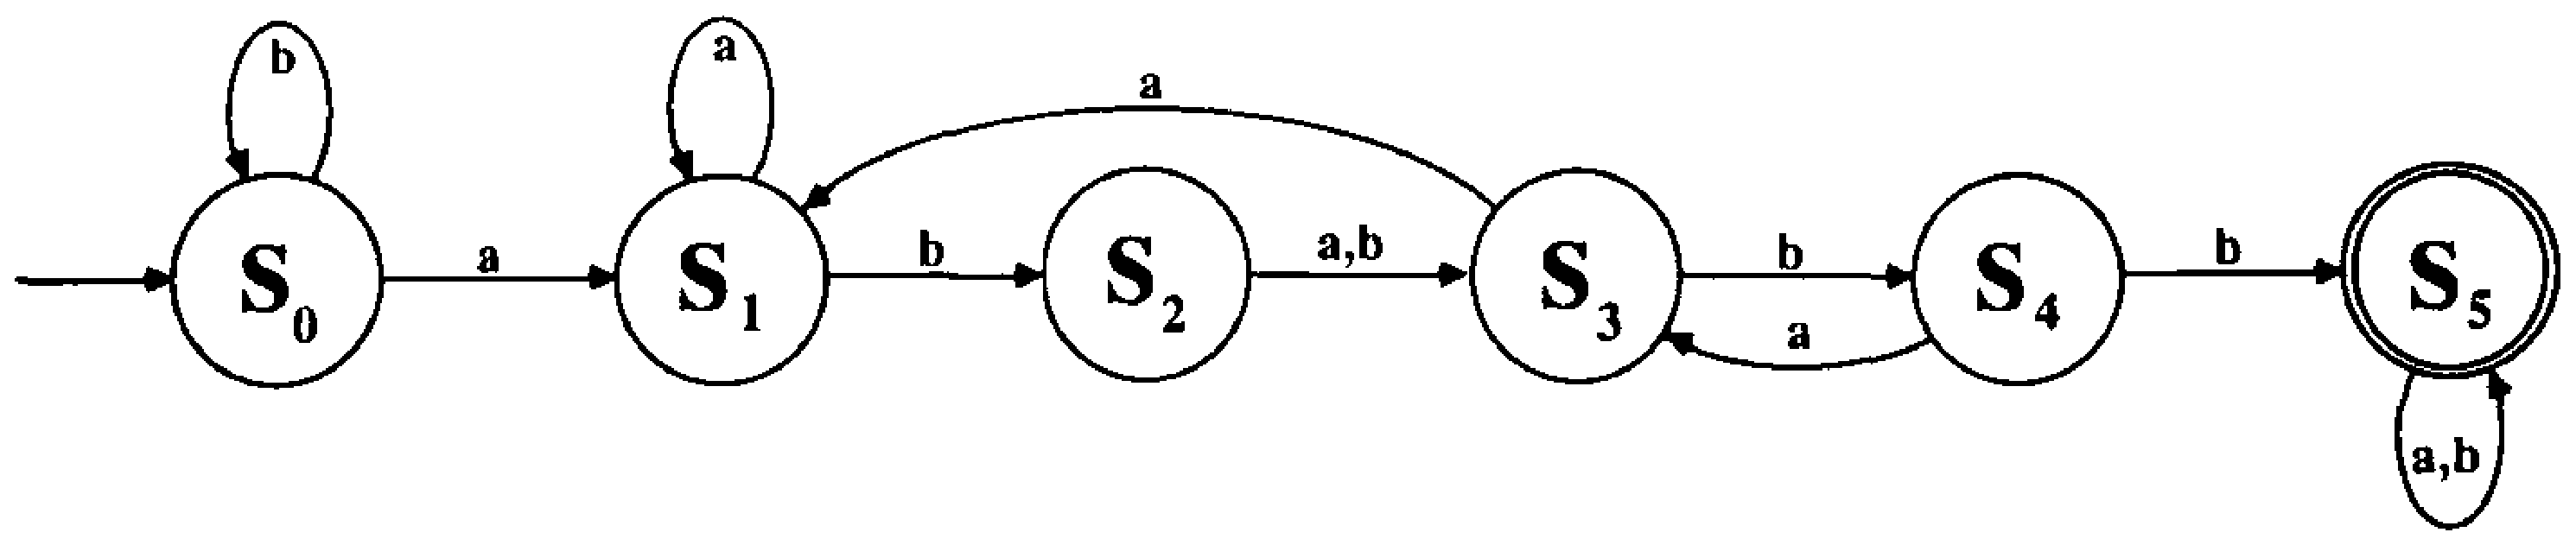
\epsfig{figure=ToFAfigures/fig1-24.eps,width=6.5in}}
\caption{A DFA that accepts strings that contain either $\pmb{ababb}$ or
$\pmb{abbbb}$}\label{fig-1.24}
\end{figure}
In this case, we required one letter between the initial part of the search
string ($\pmb{ab}$) and the terminal part ($\pmb{bb}$). It is possible to modify
the machine to accept strings that contain $\pmb{ab}$, followed by any number of
letters, followed by $\pmb{bb}$. This type of machine would be useful for
identifying \emph{comments} in many programming languages. For example, a Pascal
comment is essentially of the form $\pmb{(^*}$, followed by most combinations
of letters, followed by the first occurrence of $\pmb{^*)}$.

It should be noted that the machine in Example 1.15 is highly
specialized and tailored for the specific string $\pmb{ababb}$; other target
strings would require completely different recognizers. While it appears to
require much thought to generate the appropriate DFA for a given string, we will
see how the tools presented in Chapter \ref{ch-4} can be used to automate the
entire process.

Example 1.15 indicates how automata can be used to guide the construction of
software for matching designated patterns. Finite-state machines are also useful
in designing hardware that detects designated sequences. Example 4.7 will
explore a communications application, and the following discussion illustrates
how these concepts can be applied to help evaluate the performance of computers.

A computer program is essentially a linear list of machine instructions, stored
in consecutive memory locations. Each memory location holds a sequence of bits
that can be thought of as words comprised of $\pmb{0}$s and $\pmb{1}$s.
Different types of instructions are represented by different patterns of bits.
The CPU sequentially \emph{fetches} these instructions and chooses its next
action by examining the incoming bit pattern to determine the type of
instruction that should be executed. The sequences of bits that encode the
instruction type are called \emph{\Index{opcodes}}.

Various performance advantages can be attained when one part of the CPU
\emph{prefetches} the next instruction while another part executes the current
instruction. However, computers must have the capability of altering the order
in which instructions are executed; \emph{branch} instructions \index{branch instructions} allow the
CPU to avoid the anticipated next instruction and instead begin executing the
instructions stored in some other area of memory. When a branch occurs, the
prefetched instruction will generally need to be replaced by the proper
instruction from the new area of memory. The consequent delay can degrade the
speed with which instructions are executed.

Irrespective of prefetching problems, it should be clear that a branch
instruction followed immediately by another branch instruction is inefficient.
If a CPU is found to be regularly executing two or more consecutive branch
instructions, it may be worthwhile to consider replacing such series of branches
with a single branch to the ultimate destination [FERR]. Such information would
be determined by monitoring the instruction stream and searching for patterns
that represented consecutive branch opcodes. This activity is essentially the
pattern recognition problem discussed in Example 1.15.

It is unwise to try to collect the data representing the contents of the
instruction stream on secondary storage so that it can be analyzed later. The
volume of information and the speed with which it is generated preclude the
collection of a sufficiently large set of data points. Instead, the preferred
solution uses a specially tailored piece of hardware to monitor the contents of
the CPU opcode register and increment a hardware counter each time the
appropriate patterns are detected. The heart of this monitor can be built by
transforming the appropriate automaton into the corresponding logic circuitry,
as outlined in Section \ref{sec-1.4}. Unlike the automaton in Example 1.15,
the automaton model for this application would allow transitions out of the final
state, so that it may continue to search for successive patterns. The resulting
logic circuitry would accept as input the bit patterns currently present in the
opcode register, and send a pulse to the counter mechanism each time the accept
circuitry was energized.

Note that in this case we would not want to inhibit the accept circuitry by
requiring an \<EOS\> symbol to be scanned. Indeed, we want the light on our
conceptual black box to flicker as we process the data, since we are intent on
counting the number of times it flickers during the course of our monitoring.

\subsection*{Example 1.16}

We close this chapter with an illustration of the manner in which computational
algorithms can profitably use the automaton abstraction. Network communications
between independent processors are governed by a \emph{\Index{protocol}} that
implements a finite state control [TANE]. The \emph{Kermit} protocol,\index{Kermit protocol!DFA implementation}
developed at Columbia University, was widely employed to communicate between
processors and is still most often used for its original purpose: to transfer
files between micros and mainframes [DACR]. During a file transfer, the send
portion of Kermit on the source host is responsible for delivering data to the
receive portion of the Kermit process on the destination host. The receive
portion of Kermit reacts to incoming data in much the same way as the machines
presented in this chapter. The receive program \emph{starts} in a state of waiting for
a transfer request (in the form of an initialization packet) to signal the
commencement of a file transfer (state R in Figure \ref{fig-1.25}). When such
a packet is received, Kermit \emph{transitions} to the RF state, where it awaits a
file-header packet (which specifies the name of the file about to be transferred).
Upon receipt of the file-header packet, it enters the RD state, where it processes
a succession of data packets (which comprise the body of the file being
transferred). An \Index{EOF packet} should arrive after all the data are sent, which can
then be followed by another file-header packet (if there is a sequence of files
to be transferred) or by a break packet (if the transfer is complete). In the
latter case, Kermit reverts to the start state R and awaits the next transfer
request. The send portion of the Kermit process on the source host follows the
behavior of a slightly more complex automaton. The state transition diagram
given in Figure \ref{fig-1.25} succinctly describes the logic of the receive
portion of the Kermit protocol; for simplicity, timeouts and error conditions
are not reflected in the diagram. The input alphabet is \{B,D,Z,H,S\}, where B
represents a break, D is a data packet, Z is EOF, H is a file-header packet, and
S is a send-intention packet. The state set is \{A,R,RF,RD\}, where A denotes
the \underline{\emph{a}}bort state, R signifies \underline{\emph{r}}eceive,
RF is \underline{\emph{r}}eceive \underline{\emph{f}}ileheader, and RD is
\underline{\emph{r}}eceive \underline{\emph{d}}ata. Note that unexpected packets (such as a data packet received in
the start state R or a break packet received when data packets are expected in
state RD) cause a transition to the abort state A.

% Figure 1.25
\begin{figure}
\centerline{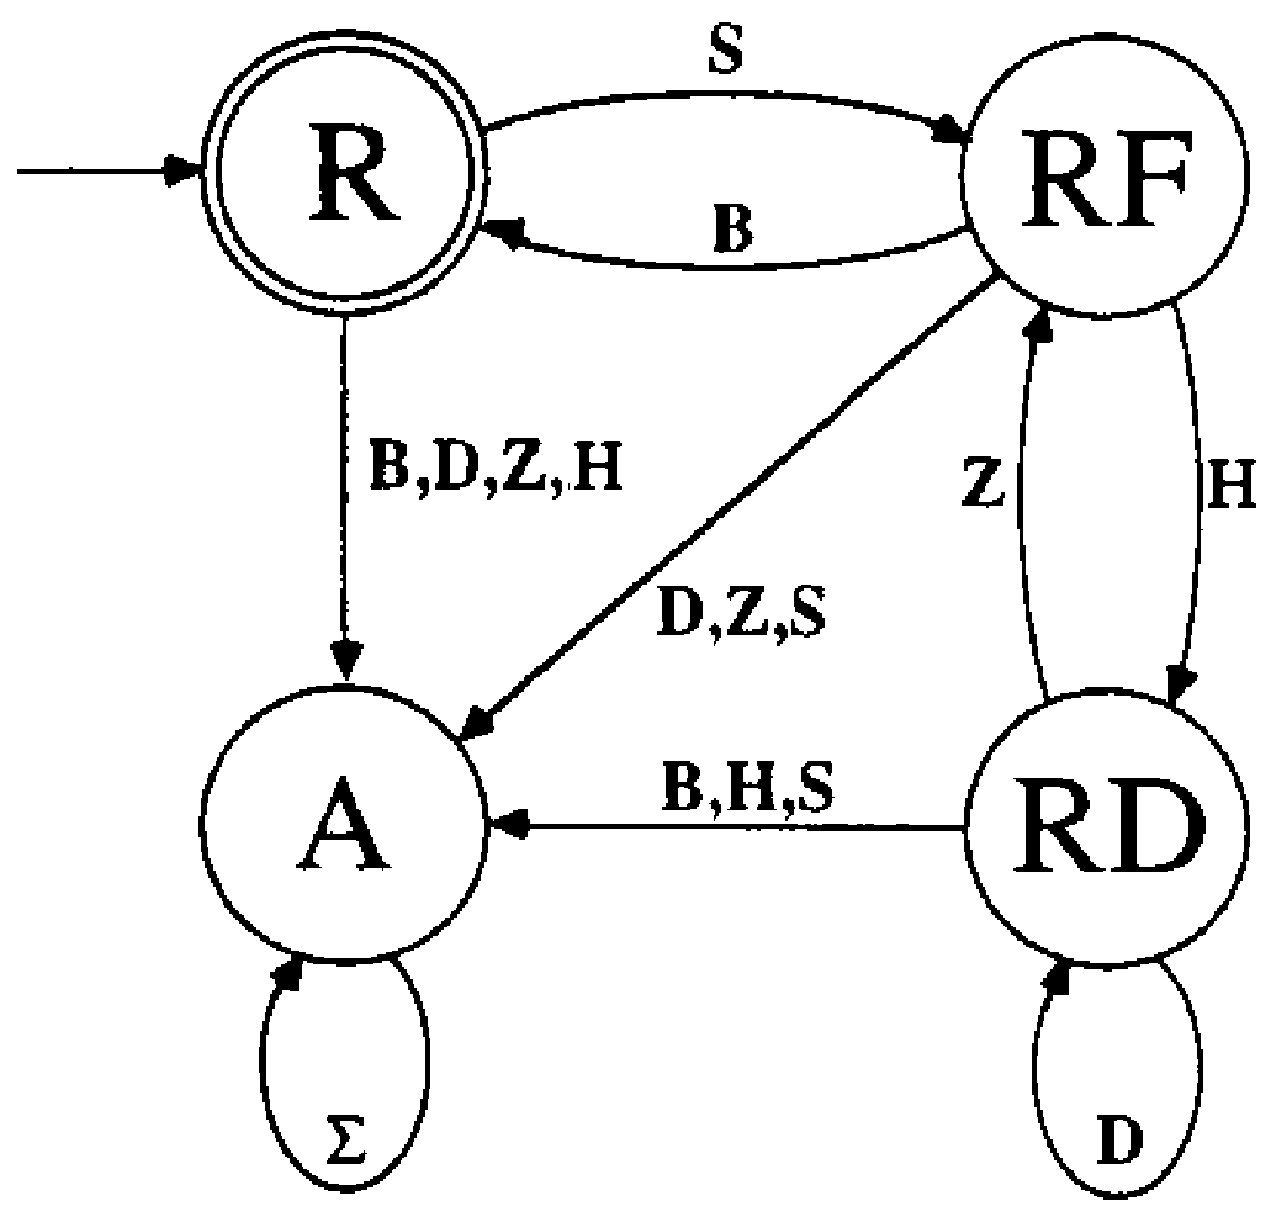
\epsfig{figure=ToFAfigures/fig1-25.eps,width=3.5in}}
\caption{The state transition diagram for the receive portion of Kermit, as
discussed in Example 1.16}\label{fig-1.25}
\end{figure}

In actuality, the receive protocol does more than just observe the incoming
packets; Kermit sends an acknowledgment (ACK or NAK)\index{ACK|see{Kermit protocol}}\index{NAK|see{Kermit protocol}} of each packet back to
the source host. Receipt of the file header should also cause an appropriate
file to be created and opened, and each succeeding data packet should be
verified and its contents placed sequentially in the new file. A machine model
that incorporates actions in response to input is the subject of Chapter \ref{ch-7},
where automata with output are explored.

\section*{EXERCISES}\label{sec-1.ex}

\begin{enumerate}[{1.}1.]
\item Recall how we defined $\DBAR$ in this chapter:
\begin{center}\begin{tabular}{l@{$\qquad$}l}
$(\forall s\in S)(\forall\pmb{a}\in \Sigma)$ & $\DBAR_t(s,\pmb{a})=\delta(s,
	\pmb{a})$ \\
$(\forall s\in S)$ & $\DBAR_t(s,\lambda)=s$ \\
$(\forall s\in S)(\forall x\in\Sigma^*)(\forall\pmb{a}\in\Sigma)$ & $\DBAR_t
	(s,\pmb{a}x)=\DBAR_t(\delta(s,\pmb{a}),x)$
\end{tabular}\end{center}
$\DBAR$, here denoted $\DBAR_t$, was tail recursive. Tail recursion means that
all recursion takes place at the end of the string. Let us now define an
alternative extended transition function, $\DBAR_h$, thusly:
\begin{center}\begin{tabular}{l@{$\qquad$}l}
$(\forall s\in S)(\forall\pmb{a}\in\Sigma)$ & $\DBAR_h(s,\pmb{a})=\delta(s,
	\pmb{a})$ \\
$(\forall s\in S)$ & $\DBAR_h(s,\lambda)=s$ \\
$(\forall s\in S)(\forall\pmb{a}\in\Sigma)(\forall x\in\Sigma^*)$ & $\DBAR_h
	(s,x\pmb{a})=\delta(\DBAR_h(s,x),\pmb{a})$
\end{tabular}\end{center}
It is clear from the definition of $\DBAR_h$ that all the recursion
takes place at the head of the string. For this reason, $\DBAR_h$ is
called \emph{\Index{head recursive}}. Show that the two definitions result in
the same extension of $\delta$, that is, prove by mathematical induction that
\[ (\forall s\in S)(\forall x\in\Sigma^*)(\DBAR_t(s,x)=\DBAR_h(s,x)) \]

\item Consider Example 1.14. The vending machine accepts coins as input, but if
you change your mind (or find you do not have enough change), it will not
refund your money. Modify this example to have another input, \<coin-return\>,
which is represented by $\pmb{r}$ and which will conceptually return all your
coins.

\item\label{exer1.3}
\begin{enumerate}
  \item Specify the quintuple corresponding to the DFA displayed in Figure \ref{fig-1.26}.
  \item Describe the language defined by the DFA displayed in Figure \ref{fig-1.26}.
\end{enumerate}

% Figure 1.26
\begin{figure}[h]
\centerline{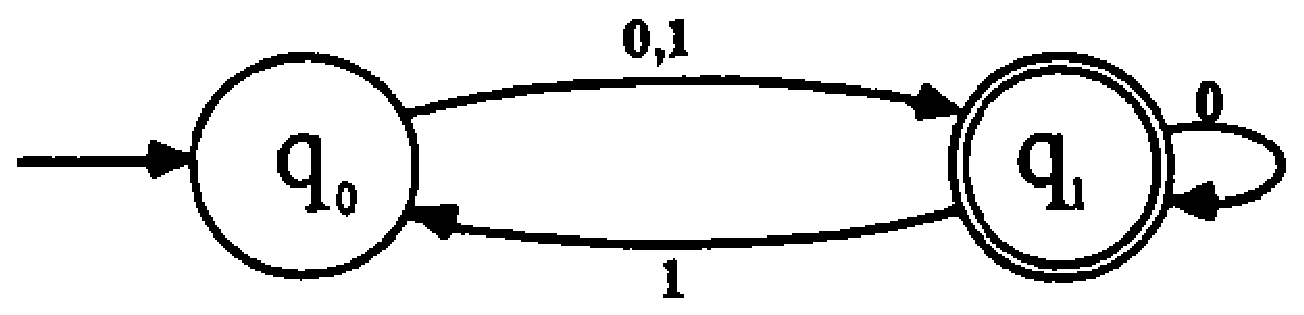
\epsfig{figure=ToFAfigures/fig1-26.eps,width=3.5in}}
\caption{The automaton discussed in Exercise 1.\ref{exer1.3}}\label{fig-1.26}
\end{figure}

\item Construct a state transition diagram and enumerate all five parts of a
deterministic finite automaton $A=\langle\{\pmb{a},\pmb{b},\pmb{c}\},S,s_0,
\delta,F\rangle$ such that
\[ L(A) = \{x \ | \ \ \ |x|\text{ is a multiple of }2\text{ or }3\}. \]

\item Let $\Sigma = \{\pmb{0},\pmb{1}\}$. Construct deterministic finite
automata that will accept each of the following languages, if possible.
\begin{enumerate}
\item $L_1=\{x \ |\ \ \ |x| \bmod 7 = 4\}$
\item $L_2=\Sigma^*-\{w\ | \ \exists n\geq 1\ni w=\pmb{a}_1\ldots \pmb{a}_n\wedge \pmb{a}_n = 1\}$
\item $L_3=\{y \ | \ \ \ |y|_0=|y|_1\}$
\end{enumerate}

\item Let $\Sigma = \{\pmb{a},\pmb{b}\}$.
\begin{enumerate}
\item Construct deterministic finite automata $A_1$, $A_2$, $A_3$, and $A_4$
such that:
\begin{enumerate}
\item $L(A_1)=\{x\ |\ (|x|_a\text{ is odd})\wedge(|x|_b\text{ is even})\}$
\item $L(A_2)=\{y\ |\ (|y|_a\text{ is even})\vee(|y|_b\text{ is odd})\}$
\item $L(A_3)=\{z\ |\ (|z|_a\text{ is even})\overline{\vee}(|z|_b\text{ is even})\}
	\ \ (\overline{\vee}\text{ represents exclusive-or})$
\item $L(A_4)=\{z\ | \ \ \ |z|_a\text{ is even}\}$
\end{enumerate}
\item How does the structure of each of these machines relate to the one defined
in Example 1.10?
\end{enumerate}

\item Modify the machine $M$ defined in Example 1.10 so that the language
accepted by the machine consists of strings $x\in\{\pmb{a},\pmb{b}\}^*$, where
both $|x|_{\pmb{a}}$ and $|x|_{\pmb{b}}$ are even and $|x|>0$, that is, the new
machine should accept $L(M) - \{\lambda\}$.

\item Let $M=\langle\Sigma,S,s_0,\delta,F\rangle$ be an (arbitrary) DFA that accepts the
language $L(M)$. Write down a general procedure for modifying this machine so
that it will accept $L(M) - \{\lambda\}$. (Specify the five parts of the new
machine and justify your statements.) It may be helpful to do this for a
specific machine (as in Exercise 1.7) before attempting the general case.

\item Let $M=\langle\Sigma,S,s_0,\delta,F\rangle$ be an (arbitrary) DFA that accepts the
language $L(M)$. Write down a general procedure for modifying this machine so
that it will accept $L(M)\cup\{\lambda\}$. (Specify the five parts of the new
machine and justify your statements.)

\item Let $\Sigma=\{\pmb{a},\pmb{b},\pmb{d}\}$ and $\Psi=\{x\in\Sigma^*
 \ | \ (x\text{ begins with }\pmb{d})\vee(x\text{ contains two consecutive $\pmb{b}$s})\}$.
\begin{enumerate}
\item Draw a machine that will accept $\Psi$.
\item Formally specify the five parts of the DFA from part (a).
\end{enumerate}

\item Let $\Sigma=\{\pmb{a},\pmb{b},\pmb{c}\}$ and $\Phi=\{x \in \Sigma^*
	|\text{ every $\pmb{b}$ in $x$ is immediately followed by }\pmb{c}\}$.
\begin{enumerate}
\item Draw a machine that will accept $\Phi$.
\item Formally specify the five parts of the DFA from part (a).
\end{enumerate}

\item Let $\Sigma=\{\pmb{0},\pmb{1},\pmb{2},\pmb{3},\pmb{4},\pmb{5},\pmb{6},
\pmb{7},\pmb{8},\pmb{9}\}$. Consider the base 10 numbers formed by strings from
$\Sigma^*$: $\pmb{14}$ represents fourteen, the three-digit string $\pmb{205}$
represents two hundred and five, and so on. Let $\Omega=\{x \in \Sigma^*
|$ the number represented by $x$ is evenly divisible by $7$\} = 
$\{\lambda,\pmb{0},\pmb{00},\pmb{000},\ldots,\pmb{7},\pmb{07},\pmb{007},\ldots,
\pmb{14},\pmb{21},\pmb{28},\pmb{35},\ldots\}$.
\begin{enumerate}
\item Draw a machine that will accept $\Omega$.
\item Formally specify the five parts of the DFA from part (a).
\end{enumerate}

\item Let $\Sigma=\{\pmb{0},\pmb{1},\pmb{2},\pmb{3},\pmb{4},\pmb{5},\pmb{6},
\pmb{7},\pmb{8},\pmb{9}\}$. Let $\Gamma=\{x\in \Sigma^*|$ the number represented
by $x$ is evenly divisible by $3$\}.
\begin{enumerate}
\item Draw a three-state machine that will accept $\Gamma$.
\item Formally specify the five parts of the DFA from part (a).
\end{enumerate}

\item Let $\Sigma=\{\pmb{0},\pmb{1},\pmb{2},\pmb{3},\pmb{4},\pmb{5},\pmb{6},
\pmb{7},\pmb{8},\pmb{9}\}$. Let $K=\{x\in \Sigma^*|$ the number represented by
$x$ is evenly divisible by $5$\}.
\begin{enumerate}
\item Draw a five-state DFA that accepts $K$.
\item Formally specify the five parts of the DFA from part (a).
\item Draw a two-state DFA that accepts $K$.
\item Formally specify the five parts of the DFA from part (c).
\end{enumerate}

\item Let $\Sigma=\{\pmb{0},\pmb{1},\pmb{2},\pmb{3},\pmb{4},\pmb{5},\pmb{6},
\pmb{7},\pmb{8},\pmb{9}\}$. Draw a DFA that accepts the first eight primes.

\item \begin{enumerate}
\item Find all ten combinations of $u$, $v$, and $w$ such
that $uvw=\pmb{cab}$ (one such combination is $u=\pmb{c}$, $v=\lambda$,
$w=\pmb{ab}$).
\item In general, if $x$ is of length $n$, and $uvw = x$, how many distinct
combinations of $u$, $v$, and $w$ will satisfy this constraint?
\end{enumerate}

\item Let $\Sigma = \{\pmb{a},\pmb{b}\}$ and $\Xi =\{x \in \Sigma^*|x$ contains
(at least) two consecutive $\pmb{b}$s $\wedge\ x$ does \emph{not} contain two
consecutive $\pmb{a}$s\}. Draw a machine that will accept $\Xi$.

\item The FORTRAN identifier in Example 1.9 recognized \emph{all} alphabetic
words, including those like DO, DATA, END, and STOP, which have different uses
in FORTRAN. Modify Figure \ref{fig-1.11} to produce a DFA that will also reject
the words DO and DATA while still accepting all other valid FORTRAN identifiers.

\item Consider the machine defined in Example 1.11. This machine
accepts most real number constants in scientific notation. However, this machine
does have some (possibly desirable) limitations. These limitations include
requiring that a $\pmb{0}$ precede the decimal point when specifying a number
with a mantissa less than 1.
\begin{enumerate}
\item Modify Figure \ref{fig-1.13} so that it will accept the set of real-number
constants described by the following BNF.
\begin{center}
%\begin{tabular}{r@{ ::}l}
\begin{tabular}{rllll}
\<sign\> & $::=$ & $ \pmb{+}|\pmb{-}$ & \\
\<digit\> &  $::=$ & $ \pmb{0}|\pmb{1}|\pmb{2}|\pmb{3}|\pmb{4}|\pmb{5}|\pmb{6}|\pmb{7}|
	\pmb{8}|\pmb{9}$ & \\
\<natural\> & $::=$ & \<digit\>$|$\<digit\>\<natural\> & \\
\<integer\> & $::=$ & \<natural\>$|$\<sign\>\<natural\> & \\
\<real constant\> & $::=$& \<integer\> & $|$ \\
&& \<integer\>{\bf .} & $|$ \\
&& {\bf .}\<natural\> & $|$ \\
&& \<sign\>{\bf .}\<natural\> & $|$ \\
&& {\bf .}\<natural\>{\bf E}\<integer\> & $|$ \\
&& \<sign\>{\bf .}\<natural\>{\bf E}\<integer\> & $|$ \\
&& \<integer\>{\bf .}\<natural\> & $|$ \\
&& \<integer\>{\bf .}\<natural\>{\bf E}\<integer> & \\
\end{tabular}
\end{center}
\item Write a program in your favorite programming language to implement the
automaton derived in part (a). The program should read a line of text and state
whether or not the word on that line was accepted.
\end{enumerate}

\item Show that part (i) of Definition \ref{dfn-1.11} is implied by parts (ii)
and (iii) of that definition.

\item Develop a more succinct description of the transition function given in
Example 1.9 (compare with the description in Example 1.10).

\item Let the universal set be $\{\pmb{a,b}\}^*$. Give an example of
\begin{enumerate}
\item A finite set.
\item A cofinite\index{cofinite!set} set.
\item A set that is neither finite nor cofinite.
\end{enumerate}

\item\label{q-states} Consider the DFA given in Figure \ref{fig-1.27}.
\begin{enumerate}
\item Specify the quintuple for this machine.
\item Describe the language defined by this machine.
\end{enumerate}

% Figure 1.27
\begin{figure}
\centerline{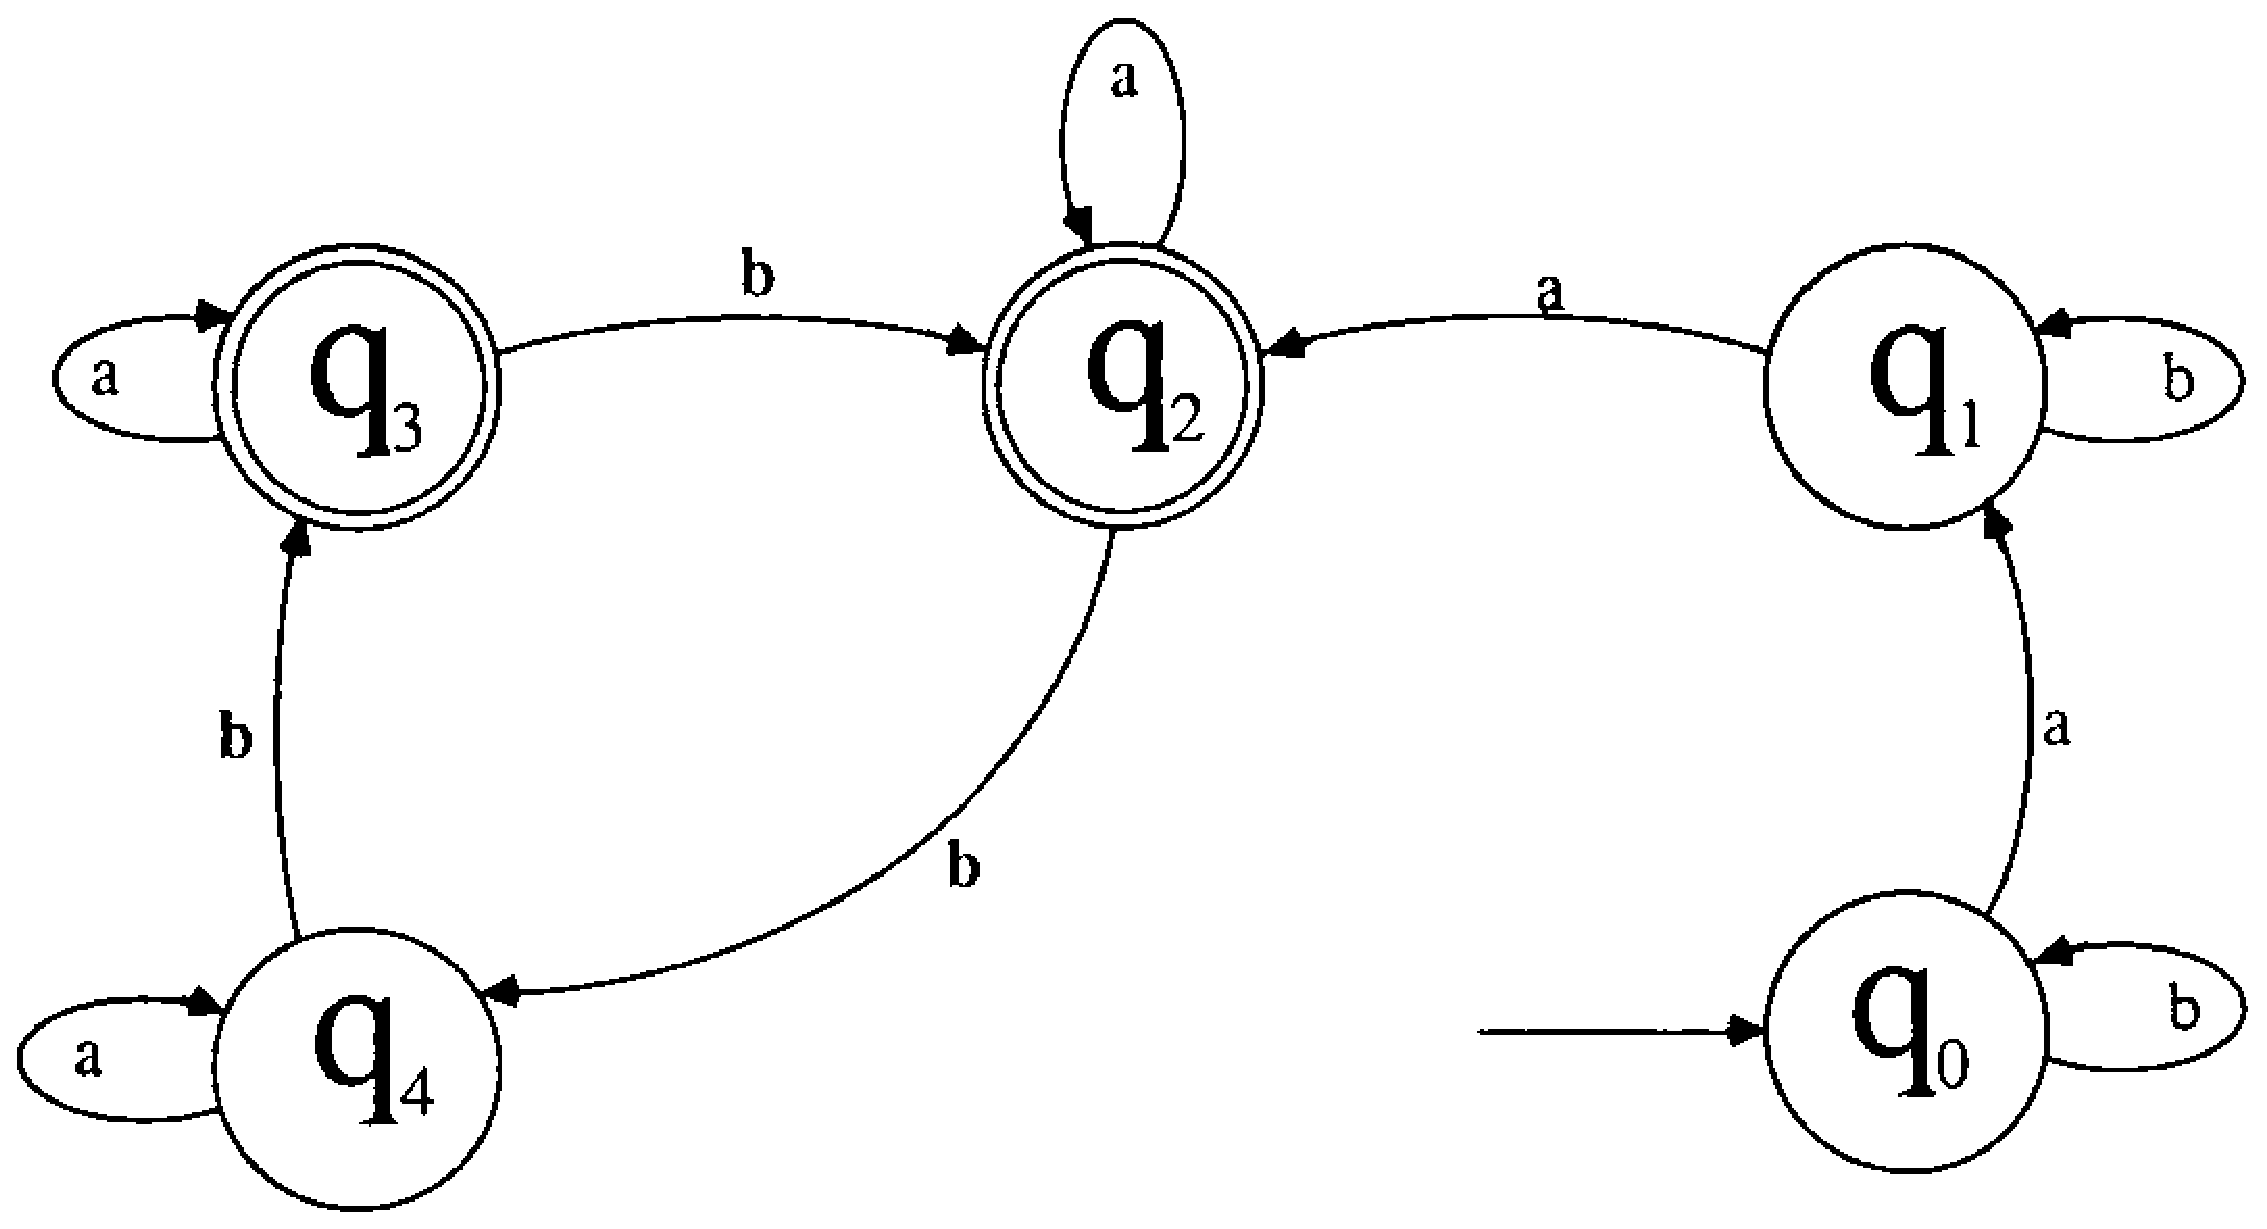
\epsfig{figure=ToFAfigures/fig1-27.eps,width=5in}}
\caption{The DFA discussed in Exercise 1.\ref{q-states}}\label{fig-1.27}
\end{figure}

\item Consider the set consisting of the names of everyone in China. Is this set
a FAD language?

\item Consider the set of all legal infix arithmetic expressions over the
alphabet $\{\pmb{A},\pmb{B},\pmb{+},\pmb{-},\pmb{\times},\pmb{/}\}$ without
parentheses (assume normal precedence rules apply). Is this set a FAD language?
If so, draw the machine.
(Assume that $\pmb{-}$ represents both negation and subtraction.)

\item Consider an arbitrary deterministic finite automaton $M$.
\begin{enumerate}
\item What aspect of the machine determines whether $\lambda \in L(M)$?
\item Specify a condition that would guarantee that $L(M) = \Sigma^*$.
\item Specify a condition that would guarantee that $L(M) = \emptyset$.
\end{enumerate}

\item Construct deterministic finite automata to accept each of the following
languages.
\begin{enumerate}
\item $\{x\in\{\pmb{a},\pmb{b},\pmb{c}\}^* |\  \ \pmb{abc}\text{ is a substring of }x\}$
\item $\{x\in\{\pmb{a},\pmb{b},\pmb{c}\}^* |\  \ \pmb{acaba}\text{ is a substring of }x\}$
\end{enumerate}

\item Consider Example 1.14. The vending machine had as input nickels,
dimes, and quarters. When 30\cent\  had been deposited, a candy bar could be
selected. Modify this machine to also accept pennies, denoted by $p$, as an
additional input. How does this affect the number of states in the machine?

\item\label{t-states} \begin{enumerate}
\item Describe the language defined by the following quintuple (compare with
Figure \ref{fig-1.28}).
\begin{center}\begin{tabular}{l@{$\qquad$}l}
$\Sigma=\{\pmb{a},\pmb{b}\}$ & $\delta(t_0,\pmb{a})=t_0$ \\
$S=\{t_0,t_1\}$ & $\delta(t_0,\pmb{b})=t_1$ \\
$s_0=t_0$ & $\delta(t_1,\pmb{a})=t_1$ \\
$F=\{t_1\}$ & $\delta(t_1,\pmb{b})=t_0$
\end{tabular}\end{center}
\item Rigorously \emph{prove} the statement you made in part (a). \emph{Hint:} First
prove the inductive statement
\[ P(n):(\forall x \in \Sigma^n)((\DBAR(t_0,x)=t_0\Leftrightarrow|x|_{\pmb{b}}
\text{ is even}) \wedge (\DBAR(t_0,x)=t_1\Leftrightarrow|x|_{\pmb{b}}
\text{ is odd})). \]
\end{enumerate}

% Figure 1.28
\begin{figure}
\centerline{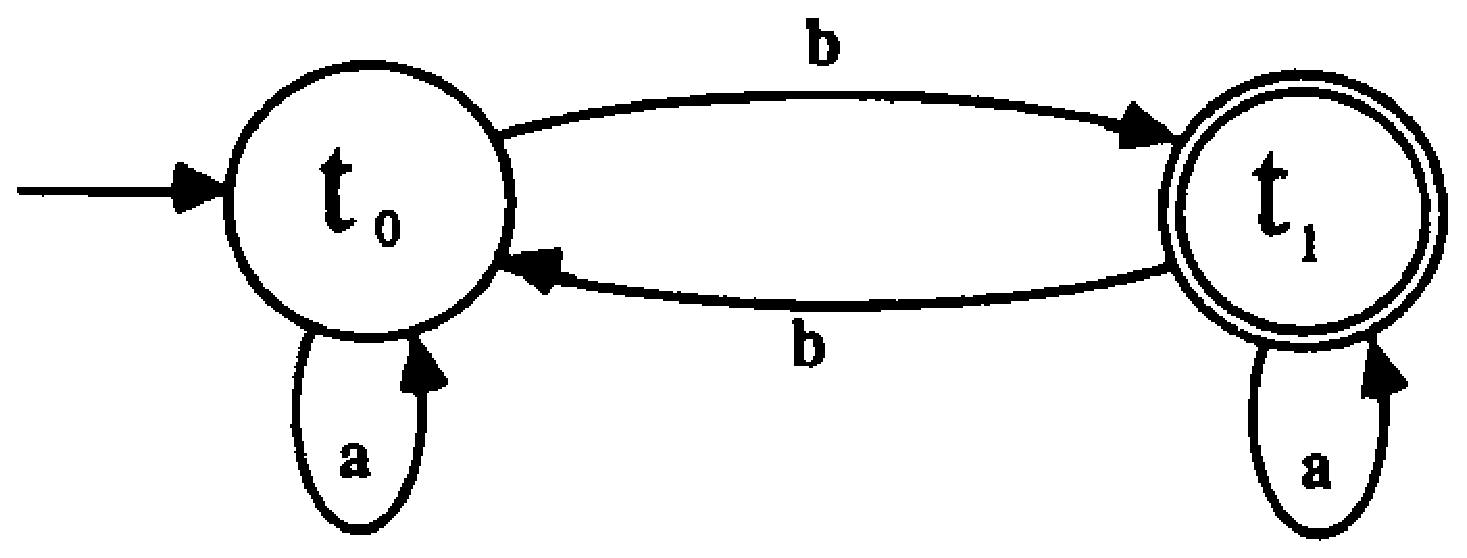
\epsfig{figure=ToFAfigures/fig1-28.eps,width=3in}}
\caption{The DFA discussed in Exercise 1.\ref{t-states}}\label{fig-1.28}
\end{figure}

\item Consider a vending machine that accepts as input pennies, nickels, dimes,
and quarters and dispenses 10\cent\  candy bars.
\begin{enumerate}
\item Draw a DFA that models this machine.
\item Define the quintuple for this machine.
\item How many states are absolutely necessary to build this machine?
\end{enumerate}

\item Consider a vending machine that accepts as input nickels, dimes, and
quarters and dispenses 10\cent\  candy bars.
\begin{enumerate}
\item Draw a DFA that models this machine.
\item How many states are absolutely necessary to build this machine?
\item Using the standard encoding conventions, draw a circuit diagram for this
machine (include \<EOS\> but not \<SOS\> in the input alphabet).
\end{enumerate}

\item Using the standard encoding conventions, draw a circuit diagram that will
implement the machine given in Exercise 1.29, as follows:
\begin{enumerate}
\item Implements both \<EOS\> and \<SOS\>.
\item Uses neither \<EOS\> nor \<SOS\>.
\end{enumerate}

\item Using the standard encoding conventions, draw a circuit diagram that will
implement the machine given in Exercise 1.7, as follows:
\begin{enumerate}
\item Implements both \<EOS\> and \<SOS\>.
\item Uses neither \<EOS\> nor \<SOS\>.
\end{enumerate}

\item Modify Example 1.12 so that it correctly handles the \<SOS\> symbol; draw
the new circuit diagram.

\item Using the standard encoding conventions, draw a circuit diagram that will
implement the machine given in Example 1.6, as follows:
\begin{enumerate}
\item Implements both \<EOS\> and \<SOS\>.
\item Uses neither \<EOS\> nor \<SOS\>.
\end{enumerate}

\item Using the standard encoding conventions, draw a circuit diagram that will
implement the machine given in Example 1.10, as follows:
\begin{enumerate}
\item Implements both \<EOS\> and \<SOS\>.
\item Uses neither \<EOS\> nor \<SOS\>.
\end{enumerate}

\item Using the standard encoding conventions, draw a circuit diagram that will
implement the machine given in Example 1.14 (include \<EOS\> but not \<SOS\> in
the input alphabet).

\item Using the standard encoding conventions, draw a circuit diagram that will
implement the machine given in Example 1.16; include the \<SOS\> and \<EOS\>
symbols.

\item Let $\Sigma=\{\pmb{a},\pmb{b},\pmb{c}\}$. Let $L=\{x\in\{\pmb{a},\pmb{b},
\pmb{c}\}^* \ | \ \ |x|_{\pmb{b}} = 2\}$.
\begin{enumerate}
\item Draw a DFA that accepts $L$.
\item Formally specify the five parts of a DFA that accepts $L$.
\end{enumerate}

\item Draw a DFA accepting $\{x\in\{\pmb{a},\pmb{b},\pmb{c}\}^*|$ every $\pmb{b}$
in $x$ is eventually followed by $\pmb{c}\}$; that is, $x$ might look like
$\pmb{baabacaa}$, or $\pmb{bcacc}$, and so on.

\item Let $\Sigma =\{\pmb{a},\pmb{b}\}$. Consider the language consisting of all
words that have neither consecutive $\pmb{a}$s nor consecutive $\pmb{b}$s.
\begin{enumerate}
\item Draw a DFA that accepts this language.
\item Formally specify the five parts of a DFA that accepts $L$.
\end{enumerate}

\item Let $\Sigma=\{\pmb{a},\pmb{b},\pmb{c}\}$. Let
$L=\{x\in\{\pmb{a},\pmb{b},\pmb{c}\}^* \,| \ \ |x|_{\pmb{a}} \equiv 0 \bmod 3\}$.
\begin{enumerate}
\item Draw a DFA that accepts $L$.
\item Formally specify the five parts of a DFA that accepts $L$.
\end{enumerate}

\item Let $\Sigma=\{\pmb{a},\pmb{b},\pmb{(},\pmb{*},\pmb{)}\}$. Recall that a
Pascal comment is essentially of the form: $\pmb{(*}$ followed by most
combinations of letters followed by the first occurrence of $\pmb{*)}$. While
the appropriate alphabet for Pascal is the ASCII\index{ASCII alphabet} character set, for simplicity
we will let $\Sigma=\{\pmb{a},\pmb{b},\pmb{(},\pmb{*},\pmb{)}\}$. Note that
$\pmb{(*b(*b(a)b*)}$ is a single valid comment, since all characters prior to
the first $\pmb{*)}$ (including the second $\pmb{(*}$ ) are considered part of
the comment. Consequently, comments cannot be nested.
\begin{enumerate}
\item Draw a DFA that recognizes all strings that contain exactly one valid
Pascal comment (and no illegal portions of comments, as in $\pmb{aa(*b*)b(*a)}$, which should be rejected).
\item Draw a DFA that recognizes all strings that contain zero or more valid
(that is, unnested) Pascal comments. For example,
$\pmb{a(*b(*bb*)ba*)aa}$ and $\pmb{a(*b}$ are not valid, while
$\pmb{a()a(**)b(*ab*)}$ is valid.
\end{enumerate}

\item
\begin{enumerate}
\item Is the set of all postfix expressions over $\{\pmb{A},\pmb{B},\pmb{+},
\pmb{-},\pmb{\times},\pmb{/}\}$ with two or fewer operators a FAD language? If it
is, draw a machine.
\item Is the set of all postfix expressions over $\{\pmb{A},\pmb{B},\pmb{+},
\pmb{-},\pmb{\times},\pmb{/}\}$ with four or fewer operators a FAD language? If it
is, draw a machine.
\item Is the set of all postfix expressions over $\{\pmb{A},\pmb{B},\pmb{+},
\pmb{-},\pmb{\times},\pmb{/}\}$ with eight or fewer operators a FAD language? If it
is, draw a machine.
\item Do you think the set of \emph{all} postfix expressions over $\{\pmb{A},\pmb{B},
\pmb{+},\pmb{-},\pmb{\times},\pmb{/}\}$ is a FAD language? Why or why not?
\end{enumerate}

\item Let $\Sigma =\{\pmb{a},\pmb{b},\pmb{c}\}$. Consider the language
consisting of all words that begin and end with different letters.
\begin{enumerate}
\item Draw a DFA that accepts this language.
\item Formally specify the five parts of a DFA that accepts this language.
\end{enumerate}

\item Let $\Sigma =\{\pmb{a},\pmb{b},\pmb{c}\}$.
\begin{enumerate}
\item Draw a DFA that rejects all words for which the last two letters match.
\item Formally specify the five parts of the DFA.
\end{enumerate}

\item Let $\Sigma =\{\pmb{a},\pmb{b},\pmb{c}\}$.
\begin{enumerate}
\item Draw a DFA that rejects all words for which the first two letters match.
\item Formally specify the five parts of the DFA.
\end{enumerate}

\item Prove that the empty word is unique; that is, using the definition of
equality of strings, show that if $x$ and $y$ are empty words then $x = y$.

\item For any two strings $x$ and $y$, show that $|xy| = |x| + |y|$

\item \begin{enumerate}
\item Draw the DFA corresponding to
$C=\langle\{\pmb{a},\pmb{b},\pmb{c}\},\{t_0,t_1\},t_0,\delta,\{t_1\}\rangle$,
where
\begin{center}\begin{tabular}{l@{$\qquad$}l}
$\delta(t_0,\pmb{a})=t_0$ & $\delta(t_1,\pmb{a})=t_0$ \\
$\delta(t_0,\pmb{b})=t_1$ & $\delta(t_1,\pmb{b})=t_1$ \\
$\delta(t_0,\pmb{c})=t_1$ & $\delta(t_1,\pmb{c})=t_0$
\end{tabular}\end{center}
\item Describe $L(C)$.
\item Using the standard encoding conventions, draw a circuit diagram for this
machine (include \<EOS\> but not \<SOS\> in the input alphabet).
\end{enumerate}

\item Let $\Sigma=\{\pmb{I},\pmb{V},\pmb{X},\pmb{L},\pmb{C},\pmb{D},\pmb{M}\}$.
Recall that $\pmb{VVI}$ is not considered to be a Roman numeral.
\begin{enumerate}
\item Draw a DFA that recognizes strict-order Roman numerals; that is, 9 must be
represented by $\pmb{VIIII}$ rather than $\pmb{IX}$, and so on.
\item Draw a DFA that recognizes the set of all Roman numerals; that is, 9 can
be represented by $\pmb{IX}$, 40 by $\pmb{XL}$, and so on.
\item Write a Pascal program based on your answer to part (b) that recognizes
the set of all Roman numerals.
\end{enumerate}

\item Describe the set of words accepted by the DFA in Figure \ref{fig-1.9}.

\item Let $\Sigma=\{\pmb{0},\pmb{1},\pmb{2},\pmb{3},\pmb{4},\pmb{5},\pmb{6},
\pmb{7},\pmb{8},\pmb{9}\}$. Let \\
$L_n=\{x \in \Sigma^* \ | \ $ the sum of the digits of $x$ is evenly divisible by
$n$\}. Thus, \\
$L_7=\{\lambda,\pmb{0},\pmb{7},\pmb{00},\pmb{07},\pmb{16},\pmb{25},\pmb{34},
\pmb{43},\pmb{52},\pmb{59},\pmb{61},\pmb{68},\pmb{70},\pmb{77},\pmb{86},\pmb{95},
\pmb{000},\pmb{007},\ldots\}$.
\begin{enumerate}
\item Draw a machine that will accept $L_7$.
\item Formally specify the five parts of the DFA given in part (a).
\item Draw a machine that will accept $L_3$.
\item Formally specify the five parts of the DFA given in part (c).
\item Formally specify the five parts of a DFA that will recognize $L_n$.
\end{enumerate}

\item Consider the last row of Table \ref{tbl-1.3}. Unlike the preceding three
rows, the outputs in this row are not marked with the don't-care symbol. Explain.

\end{enumerate}

\chapter{Characterization of Finite Automaton Definable Languages}\label{ch-2}

Programming languages can be thought of, in a limited sense, as
conforming to the definition of a language given in Chapter \ref{ch-1}.
We can consider a text file as being one long ``word,'' that is, a
string of characters (including spaces, carriage returns, and so
on). In this sense, each Pascal program can be thought of as a
single word over the ASCII alphabet. We might define the \emph{language}
Pascal as the \emph{set} of all valid Pascal programs (that is, the valid
``words'' are those text files that would compile with no compiler
errors). This and many other languages are too complicated to be
represented by the machines described in Chapter \ref{ch-1}. Indeed,
even reliably matching an unlimited number of begin and end statements
in a file is beyond the capabilities of a DFA.

The goals for this chapter are to develop some tools for identifying
these non-FAD languages and to investigate the underlying structure
of finite automaton definable languages. We begin with the exploration
of the relations that describe that structure.

% 2.1 RIGHT CONGRUENCES
\section{Right Congruences}\label{sec-2.1}

To characterize the structure of FAD languages, we will be dealing
with relations over $\Sigma^*$, that is, we will relate strings to
other strings.  Recall that an \emph{equivalence relation} must be
\emph{reflexive, symmetric}, and \emph{transitive}. The \emph{identity}
relation over $\Sigma^*$, in which each string is related to itself
but to no other string, is an example of an equivalence relation.

The main tool we will need to understand which kinds of languages
can be represented by finite automata is the concept of a \emph{right
congruence}. If we allow the set of all strings that terminate in
some given state to define an \emph{equivalence class}, the states
of a DFA naturally partition $\Sigma^*$ into equivalence classes
(as formally presented later in Definition \ref{dfn-2.4}). Due to
the structure imposed on the machine, these classes have special
relationships that are not found in ordinary equivalence relations.
For example, if $\delta(s, a) = t$, then, given \emph{any} word $x$
in the class corresponding to the state $s$, appending an $\mathbf{a}$
to this word to form $x \mathbf{a}$ is guaranteed to produce a word
listed in the class corresponding to the state $t$. Right congruences,
defined below, allow us to break up $\Sigma^*$ in the same fashion
that a DFA breaks up $\Sigma^*$.

% Definition 2.1
\begin{dfn}\label{dfn-2.1}
Given an alphabet $\Sigma$, a relation $R$ between pairs of strings
$(R \subseteq \Sigma^* \times \Sigma^*)$ is a \emph{\Index{right congruence}} in
$\Sigma^*$ iff the following four conditions hold:
\begin{center}\begin{tabular}{lll}
$(\forall x \in \Sigma^*)$ & $(x\ R\ x)$ & $(R)$ \\
$(\forall x,y \in \Sigma^*)$ & $(x\ R\ y \Rightarrow y\ R\ x)$ & $(S)$ \\
$(\forall x,y,z \in \Sigma^*)$ & $(x\ R\ y \wedge y\ R\ z \Rightarrow x\ R\ z)$
	& $(T)$ \\
$(\forall x,y \in \Sigma^*)$ & $(x \ R\ y \Rightarrow (\forall u \in \Sigma^*)
	(xu \ R\ yu))$ & $(RC)$
\end{tabular}\end{center}
\end{dfn}

Note that if $P$ is a right congruence then the first three conditions imply
that $P$ must be an equivalence relation; for example, if $\Sigma=\{\pmb{a},
\pmb{b}\},\ \pmb{aa}\ P\ \pmb{aa}$ by reflexivity, and if $\langle\pmb{abb},
\pmb{aba}\rangle \in P$, then by symmetry $\langle\pmb{aba},\pmb{abb}\rangle
\in P$, and so forth. Furthermore, if $\pmb{abb}\ P\ \pmb{aba}$, then the right
congruence property guarantees that
\begin{center}\begin{tabular}{ll}
$\pmb{abba}\ P\ \pmb{abaa}$ & if $u = \pmb{a}$ \\ 
$\pmb{abbb}\ P\ \pmb{abab}$ & if $u = \pmb{b}$ \\
$\pmb{abbaa}\ P\ \pmb{abaaa}$ & if $u = \pmb{aa}$ \\
$\pmb{abbbbaabb}\ P\ \pmb{ababbaabb}$ & if $u = \pmb{bbaabb}$ \\
\end{tabular}\end{center}
and so on. Thus, the presence of just one ordered pair in $P$ requires the
existence of many, many more ordered pairs. This might seem to make right
congruences rather rare objects; there are, however, an infinite number of them,
many of them rather simple, as shown by the following examples.

\subsection*{Example 2.1}

Let $\Sigma=\{\pmb{a},\pmb{b}\}$, and let $R$ be defined by $x \ R\ y
\Leftrightarrow |x| - |y|$ is even. It is easy to show that this $R$ is an
equivalence relation (see the exercises) and partitions $\Sigma^*$ into two
equivalence classes: the even-length words and the odd-length words.
Furthermore, $R$ is a right congruence: for example, if $x=\pmb{abb}$ and
$y=\pmb{baabb}$, then $\pmb{abb}\ R\ \pmb{baabb}$, since $|x|-|y|=3-5= -2$, which
is even. Note that for \emph{any} choice of $u$, $\pmb{abb}u\ R\ \pmb{baabb}u$,
since $|xu|-|yu|$ will also be $-2$. Thus $\pmb{abb}u\ R\ \pmb{baabb}u$ for every
choice of $u$. The same is true for any other pair of words $x$ and $y$ that are
related by $R$, and so $R$ is indeed a right congruence.

\subsection*{Example 2.2}

Let $\Sigma=\{\pmb{a},\pmb{b},\pmb{c}\}$, and let $R_2$ be defined by
$x\ R_2 y \Leftrightarrow x$ and $y$ end with the same letter. It is
straightforward to show that $R_2$ is a right congruence (see the exercises)
and partitions $\Sigma^*$ into four equivalence classes: those words ending in
$\pmb{a}$, those words ending in $\pmb{b}$, those words ending in $\pmb{c}$, and
$\{\lambda\}$.

The relation $R_2$ was based on the placement of letters within words, while
Example 2.1 was based solely on the length of the words. The following
definition illustrates a way to produce a relation in $\Sigma^*$ based on a
given set of words $L$.

% Definition 2.2
\begin{dfn}\label{dfn-2.2}
Given an alphabet $\Sigma$, and a language $L \subseteq \Sigma^*$, the
\emph{\Index{relation induced by $L$}} in $\Sigma^*$, denoted by $R_L$, is
defined by
\[ (\forall x,y \in \Sigma^*)(x\ R_L\ y \Leftrightarrow (\forall u \in \Sigma^*)
	(xu \in L \Leftrightarrow yu \in L)) \]
\end{dfn}

\subsection*{Example 2.3}

Let $K$ be the set of all words over $\{\pmb{a},\pmb{b}\}$ that are of odd
length. Those strings that are in $K$ are used to define exactly which pairs of
strings are in $R_K$. For example, we can determine that $\pmb{ab}\ R_K\ 
\pmb{bbaa}$, since it is true that, for any $u \in \Sigma^*$, either
$\pmb{ab}u \notin K$ and $\pmb{bbaa}u \notin K$ (when $|u|$ is even) or
$\pmb{ab}u \in K$ and $\pmb{bbaa}u \in K$ (when $|u|$ is odd). Note that
$\pmb{ab}$ and $\pmb{a}$ are not related by $R_K$, since there are choices for $u$
that would violate the definition of $R_K:\ \pmb{ab}\lambda \notin K$ and yet
$\pmb{a}\lambda \in K$. In this case, $R_K$ turns out to be the same as the
relation $R$ defined in Example 2.1.

Recall that relations are sets of ordered pairs, and thus the claim that these
two relations are equal means that they are equal as sets; an ordered pair
belongs to $R$ exactly when it belongs to $R_K$:
\[ R = R_K\text{ \emph{iff} }(\forall x,y \in \Sigma^*)(x\ R\ y \Leftrightarrow
	x\ R_K\ y) \]
The strings $\pmb{ab}$ and $\pmb{bbaa}$ are related by $R$ in Example 2.1, and they
are likewise related by $R_K$. A similar statement is true for any other pair
that was in the relation $R$; it will be in $R_K$ also. Additionally, it can be
shown that elements that were not in $R$ will not be in $R_K$ either.

Notice that $R_K$ relates more than just the words in $K$; neither $\pmb{ab}$ nor
$\pmb{bbaa}$ belongs to $K$, and yet they were related to each other. This simple
language $K$ happens to partition $\Sigma^*$ into two equivalence classes,
corresponding to the language itself and its complement. Less trivial languages
will often form many equivalence classes. The relation $R_L$ defined by a
language $L$ has all the properties given in Definition \ref{dfn-2.1}.

% Theorem 2.1
\begin{thm}\label{thm-2.1}
Let $\Sigma$ be an alphabet. If $L$ is any language over $\Sigma$ (that is,
$L \subseteq \Sigma^*$), the relation $R_L$ given in Definition \ref{dfn-2.2} must be a
right congruence.

\emph{Proof.} See the exercises.
\end{thm}

Note that the above theorem is very broad in scope: \emph{any} language, no matter
how complex, \emph{always} induces a relation that satisfies all four properties
of a right congruence. Thus, $R_L$ always partitions $\Sigma^*$ into equivalence
classes. One useful measure of the complexity of a language $L$ is the degree to
which it fragments $\Sigma^*$, that is, the number of equivalence classes in
$R_L$.

% Definition 2.3
\begin{dfn}\label{dfn-2.3}
Given an equivalence relation $P$, the \emph{\Index{rank} of} $P$, denoted
$rk(P)$, is defined to be the number of \emph{distinct} (and nonempty)
equivalence classes of $P$.
\end{dfn}

The ranks of the relation in Example 2.3 was 2, since there were two equivalence
classes, the set of even-length words and the set of odd-length words. In
Example 2.2, $rk(R_2)=4$. The rank of $R_L$ can be thought of as a measure of
the complexity of the underlying language $L$. Thus, for $K$ in Example 2.3,
$rk(R_K)=2$, and $K$ might consequently be considered to be a relatively simple
language. Some languages are too complex to be recognized by finite automata;
this relationship will be explored in the subsequent sections.

While the way in which a language gives rise to a partition of $\Sigma^*$ may
seem mysterious and highly nonintuitive, a deterministic finite automaton
naturally distributes the words of $\Sigma^*$ into equivalence classes. The
following definition describes the manner in which a DFA partitions $\Sigma^*$.

% Definition 2.4
\begin{dfn}\label{dfn-2.4}
Given a DFA $M=\langle\Sigma,S,s_0,\delta,F\rangle$, define a relation $R^M$ on
$\Sigma^*$ as follows:
\[ (\forall x,y \in \Sigma^*)(x\ R^M\ y \Leftrightarrow \DBAR(s_0,x) =
	\DBAR(s_0,y)) \]
\end{dfn}

$R^M$ relates all strings that, when starting at $s_0$, wind up at the same
state. It is easy to show that $R^M$ will be an equivalence relation with
(usually) one equivalence class for each state of $M$ (remember that equivalence
classes are by definition nonempty; what type of state might not have an
equivalence class associated with it?). It is also straightforward to show that
the properties of the state transition function guarantee that $R^M$ is in fact
a right congruence (see the exercises).

The equivalence classes of $R^M$ are called \emph{\Index{initial sets}} and will
be of further interest in later chapters. For a DFA $M=\langle\Sigma,S,s_0,
\delta,F\rangle$ and a given state $t$ from $M,\ I(M,t)=\{x\ |\ \DBAR(s_0,x)=t\}$.
This initial set can be thought of as the language accepted by a machine similar
to $M$, but which has $t$ as its only final state. That is, if we define
$M_t=\langle\Sigma,S,s_0,\delta,\{t\}\rangle$, then $I(M,t)=L(M_t)$.

The notation presented here allows a concise method of denoting both relations
defined by languages and relations defined by automata. It is helpful to observe
that even in the absence of context, $R_X$ indicates that a relation based on
the \emph{language} $X$ is being described (since $X$ occurs as a subscript),
while the relation $R^Y$ identifies $Y$ as a \emph{machine} (since Y occurs as a
superscript).

Just as each DFA $M$ gives rise to a right congruence $R^M$, many right
congruences $Q$ can be associated with a DFA, which will be called $A_Q$. It can
be shown that, if some of the equivalence classes of $Q$ are singled out to form
a language $L$, $A_Q$ will recognize $L$.

% Definition 2.5
\begin{dfn}\label{dfn-2.5}
Given a right congruence Q of finite rank and a language $L$ that is the union
of some of the equivalence classes of $Q$, $A_Q$ is defined by
\[ A_Q =\langle\Sigma,S_Q,s_{0_Q},\delta_Q,F_Q\rangle \]
where
\begin{center}\begin{tabular}{l}
$S_Q =\{[x]_Q\ |\ x \in \Sigma^*\}$ \\
$s_{0_Q} = [\lambda]_Q$ \\
$F_Q =\{[x]_Q\ |\ x \in L\}$
\end{tabular}\end{center}
and $\delta_Q$ is defined by
\[ (\forall x \in \Sigma^*)(\forall a \in \Sigma)(\delta_Q([x]_Q,\pmb{a}) =
	[x\pmb{a}]_Q) \]
\end{dfn}

Note that this is a \emph{finite}-state machine since $rk(Q) < \infty$, and that
if $L_1$ were a different collection of equivalence classes of $Q$, $A_Q$ would
remain the same except for the placement of the final states. In other words,
$F_Q$ is the only aspect of this machine that depends on the language $L$ (or
$L_1$). As small as this change might be, it should be noted that $A_Q$ is
defined both by $Q$ and the language $L$. It is left for the reader to show that
$A_Q$ is well-defined and that $L(A_Q)=L$ (see the exercises). The corresponding
statements will be proved in detail in the next section for the important
special case where $Q = R_L$.

\subsection*{Example 2.4}

Let $Q \subseteq \{\pmb{a}\}^* \times \{\pmb{a}\}^*$ be the equivalence relation
with the following equivalence classes:
\begin{center}\begin{tabular}{rcl}
$[\lambda]_Q$\!\!\!\!\! & $=$ &\!\!\!\!\! $\{\lambda\}=\{\lambda\}^0$ \\
$[\pmb{a}]_Q$\!\!\!\!\! & $=$ &\!\!\!\!\! $\{\pmb{a}\}=\{\pmb{a}\}^1$ \\
$[\pmb{aa}]_Q$\!\!\!\!\! & $=$ &\!\!\!\!\! $\{\pmb{a}\}^2 \cup \{\pmb{a}\}^3 \cup \{\pmb{a}\}^4 \cup
	\{\pmb{a}\}^5 \cup \ldots$
\end{tabular}\end{center}
It is easy to show that $Q$ is a right congruence (see the exercises). If $L_1$
were defined to be $[\lambda]_Q \cup [\pmb{a}]_Q$, then $A_Q$ would have the
structure shown in Figure \ref{fig-2.1}a. For the language defined by the different
combination of equivalence classes given by $L_2=[\lambda]_Q \cup [\pmb{aa}]_Q$,
$A_Q$ would look like the DFA given in Figure \ref{fig-2.1}b. This example illustrates
that it is the right congruence $Q$ that establishes the start state and the
transitions, while the language $L$ determines the final state set. It should
also be clear why $L$ must be a union of equivalence classes from $Q$. The
figure shows that a machine with the structure imposed by $Q$ cannot possibly
both reject $\pmb{aaa}$ and accept $\pmb{aaaa}$. Either the entire equivalence class
for $[\pmb{aa}]_Q$ must belong to $L$, or none of the strings from
$[\pmb{aa}]_Q$ can belong to $L$.

% Figure 2.1
\begin{figure}
\centerline{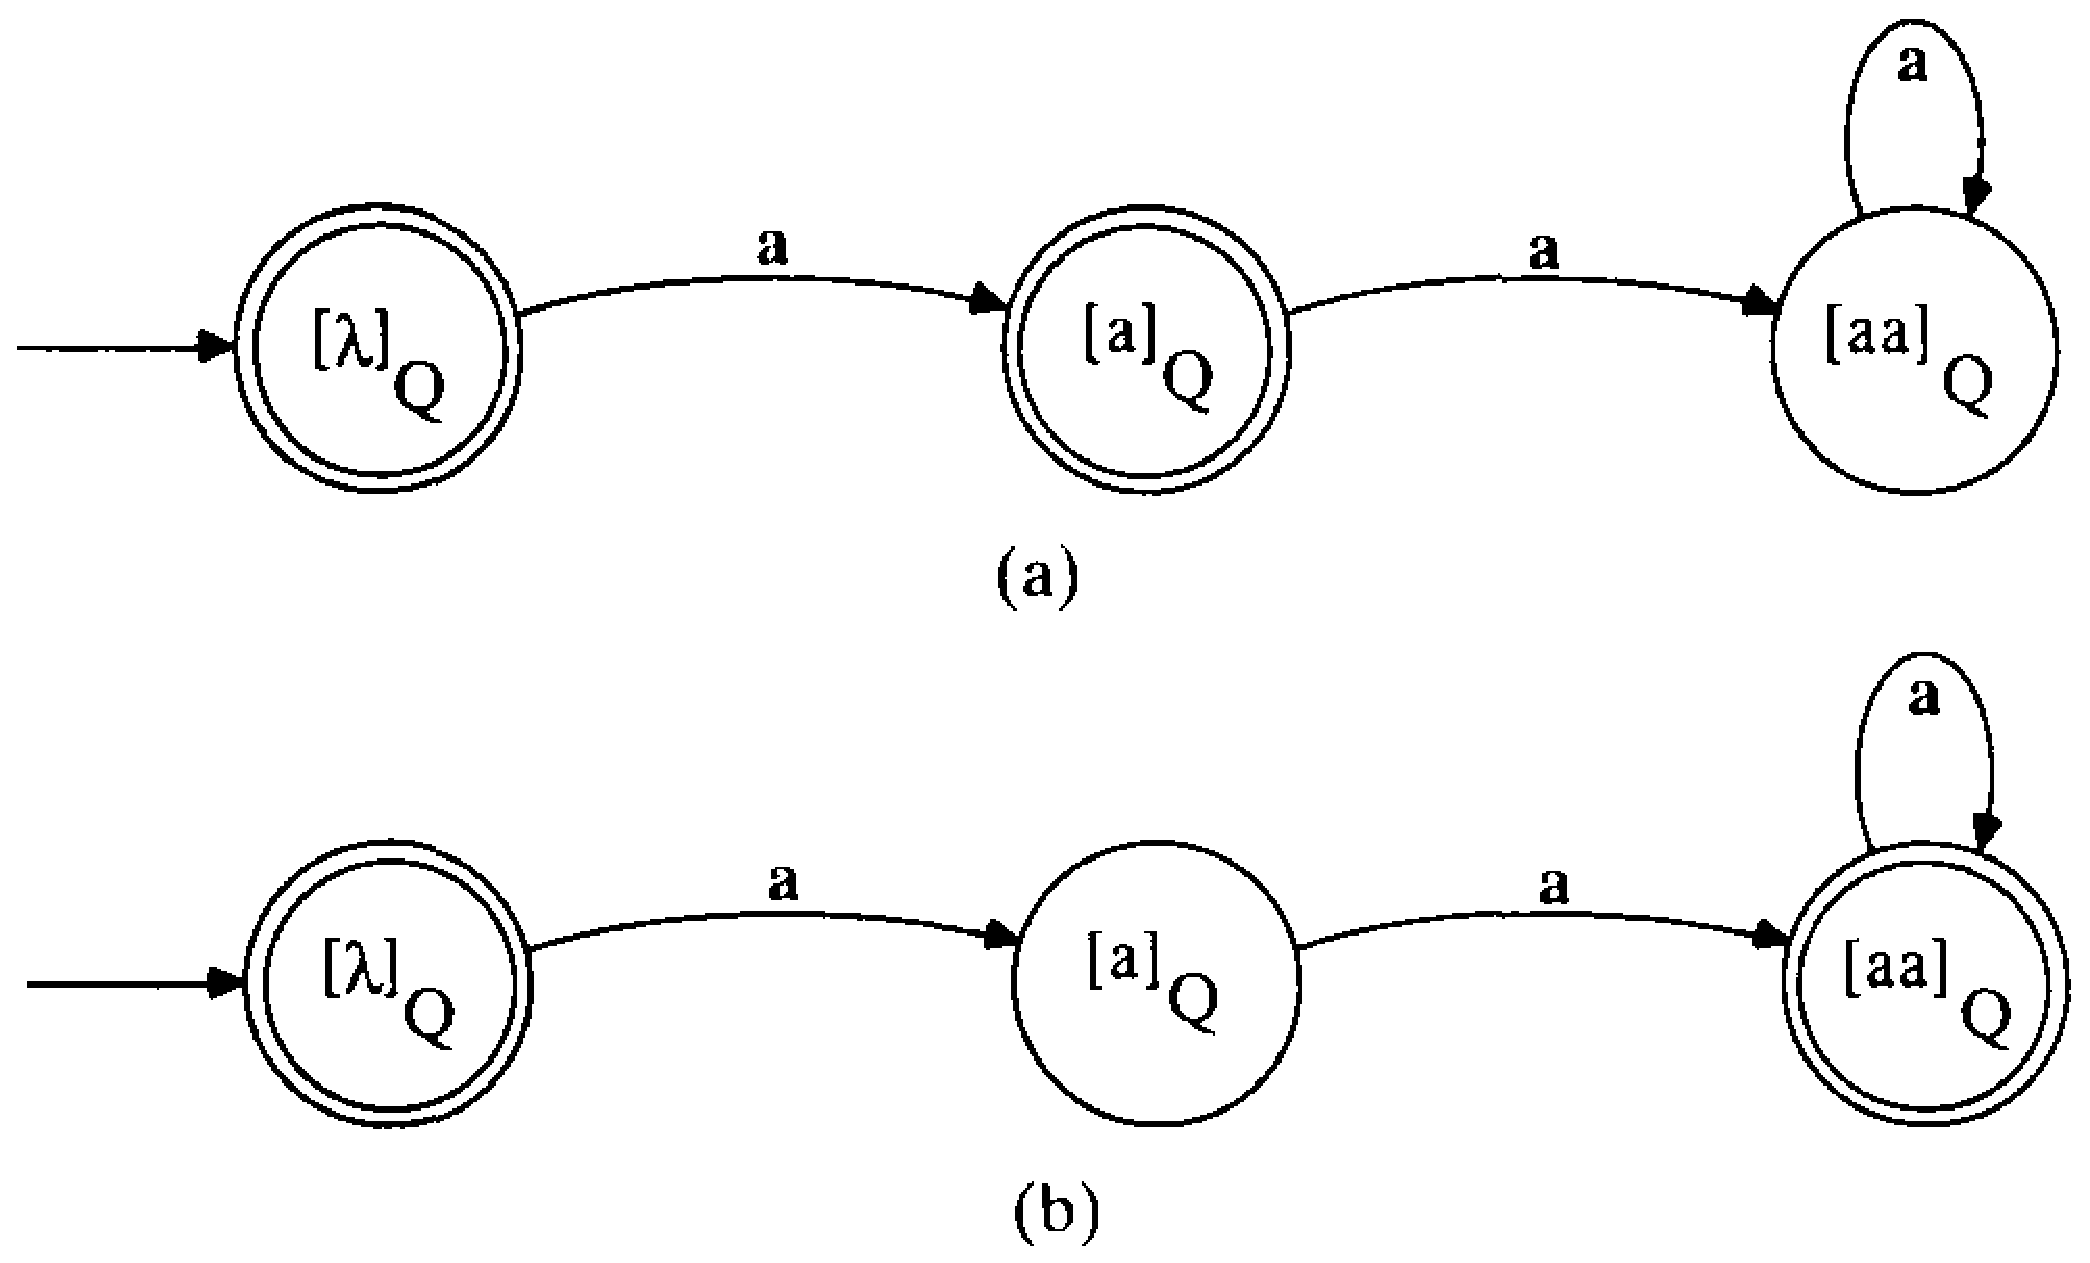
\epsfig{figure=ToFAfigures/fig2-1.eps,width=4in}}
\caption{(a) The automaton for $L_1$ in Example 2.4 (b) The automaton for $L_2$
in Example 2.4}\label{fig-2.1}
\end{figure}

\section{Nerode's Theorem}\label{sec-2.2}

In this section, we will show that languages that partition $\Sigma^*$ into a
finite number of equivalence classes can be represented by finite automata,
while those that yield an infinite number of classes would require a machine
with an infinite number of states.

\subsection*{Example 2.5}

The language $K$ given in Example 2.3 can be represented by a finite automaton
with two states; all words that have an even number of letters eventually wind
up at state $s_0$, while all the odd words are taken by \DBAR\ to $s_1$. This
machine is shown in Figure \ref{fig-2.2}.

It is no coincidence that these states split up the words of $\Sigma^*$ into the
same equivalence classes that $R_K$ does. There is an intimate relationship
between languages that can be represented by a machine with a finite number of
states and languages that induce right congruences with a finite number of
equivalence classes, as outlined in the proof of the following theorem.

% Figure 2.2
\begin{figure}
\centerline{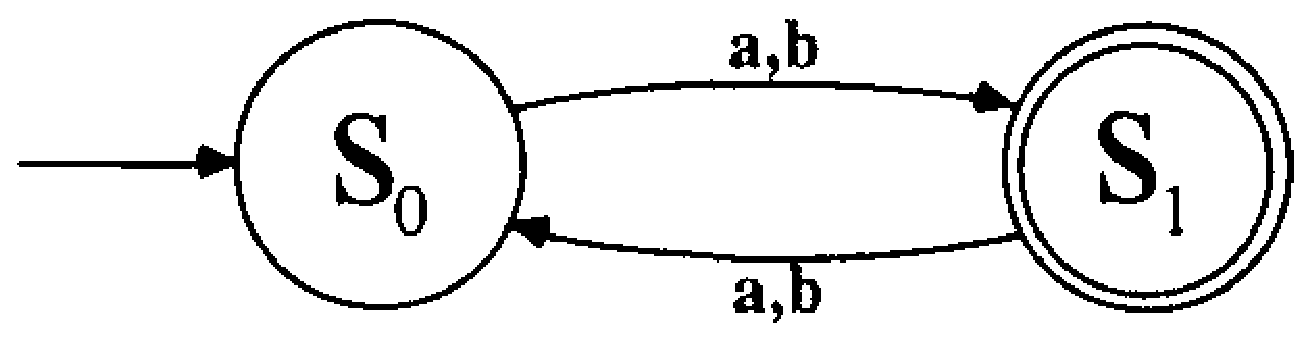
\epsfig{figure=ToFAfigures/fig2-2.eps,width=2.5in}}
\caption{The DFA discussed in Example 2.5}\label{fig-2.2}
\end{figure}

% Theorem 2.2
\begin{thm}\label{thm-2.2}
{\bf Nerode's Theorem}. Let $L$ be a language over an alphabet $\Sigma$; the
following statements are all equivalent:
\begin{enumerate}
\item $L$ is FAD.
\item There exists a right congruence $R$ on $\Sigma^*$ for which $L$ is the
(possibly empty) union of some of the equivalence classes of $R$ and $rk(R) <
	\infty$.
\item $rk(R_L) < \infty$.
\end{enumerate}

\emph{Proof.} Because of the transitivity of $\Rightarrow$, it will be
sufficient to show only the three implications (1) $\Rightarrow$ (2), (2) 
$\Rightarrow$ (3), and (3) $\Rightarrow$ (1), rather than all six of them.

\emph{Proof of} (1) $\Rightarrow$ (2): Assume (1); that is, let $L$ be FAD. Then
there is a machine that accepts $L$; that is, there exists a finite automaton
$M=\langle\Sigma,S,s_0,\delta,F\rangle$ such that $L(M) = L$. Consider the
relation $R^M$ on $\Sigma^*$ based on this machine $M$ as given in Definition
\ref{dfn-2.4}: $(\forall x,y \in \Sigma^*)(x\ R^M\ y \Leftrightarrow \DBAR(s_0,x) =
\DBAR(s_0,y))$.

This $R^M$ will be the relation $R$ we need to prove (2). For each $s \in S$,
consider $I(M,s)=\{x \in \Sigma^*\ |\ \DBAR(s_0,x) = s\}$, which represents all
strings that wind up at state $s$ (from $s_0$). Note that it is easy to define
automata for which it is impossible to reach certain states from the start
state; for such states, $I(M,s)$ would be empty. Then $\forall s \in S,\ I(M,s)$
is either an equivalence class of $R^M$ or $I(M,s)=\emptyset$. Since there is at
most one equivalence class per state, and there are a finite number of states,
it follows that $rk(R^M)$ is also finite: $rk(R^M) \leq \|S\| < \infty$.

However, we have
\[ L=L(M) = \{x \in \Sigma^*\ |\ \DBAR(s_0,x) \in F\}= \bigcup\limits_{f \in F}
	\{x \in \Sigma^*\ |\ \DBAR(s_0,x)=f\} = \bigcup\limits_{f \in F} I(M,f) \]
That is, $L$ is the union of some of the equivalence classes of the right
congruence $R^M$, and $R^M$ is indeed of finite rank, and hence (2) is
satisfied. Thus (1) $\Rightarrow$ (2).

\emph{Proof of} (2) $\Rightarrow$ (3): Assume that (2) holds; that is, there is
a right congruence $R$ for which $L$ is the union of some of the equivalence
classes of the right congruence $R$, and $rk(R) < \infty$. Note that we no
longer have (1) as an assumption; there is no machine (as yet) associated with
$L$.

{\bf Case 1}: It could be that $L$ is the empty union; that is, that
$L=\emptyset$. In this case, it is easy to show that $R_L$ has only one
equivalence class ($\Sigma^*$), and thus $rk(R_L) = 1 < \infty$ and (3) will be
satisfied.

{\bf Case 2}: In the nontrivial case, $L$ is the union of one or more of the
equivalence classes of the given right congruence $R$, and it is possible to
show that this $R$ must then be closely related to the $R_L$ induced by the
original language $L$. In particular, for any strings $x$ and $y$,
\begin{center}\begin{tabular}{rcl}
$x R\ y$ & $\Rightarrow$ & (since $R$ is a right congruence) \\
$(\forall u \in \Sigma^*)(xu\ R\ yu)$ & $\Rightarrow$ & (by definition of
	$[\ ]$) \\
$(\forall u \in \Sigma^*)([xu]_R = [yu]_R)$ & $\Rightarrow$ & (by definition of
	$L$ as a union of $[\ ]$'s) \\\
$(\forall u \in \Sigma^*)(xu \in L \Leftrightarrow yu \in L)$ & $\Rightarrow$ &
	(by definition of $R_L$) \\
$x\ R_L\ y$ &&
\end{tabular}\end{center}
$(\forall x \in \Sigma^*)(\forall y \in \Sigma^*)(x\ R\ y \Rightarrow x\ R_L\ y)$
means that $R$ refines $R_L$, and thus each equivalence class of $R$ is entirely
contained in an equivalence class of $R_L$; that is, each equivalence class of
$R_L$ must be a union of one or more equivalence classes of $R$. Thus, there are
more equivalence classes in $R$ than in $R_L$, and so $rk(R_L) \leq rk(R)$. But by
hypothesis, $rk(R)$ is finite, and so $R_L$ must be of finite rank also, and
(3) is satisfied. Thus, in either case, (2) $\Rightarrow$ (3).

\emph{Proof of} (3) $\Rightarrow$ (1): Assume now that condition (3) holds; that
is, $L$ is a language for which $R_L$ is of finite rank. Once again, note that
all we know is that $R_L$ has a finite number of equivalence classes; we do not
have either (1) or (2) as a hypothesis. Indeed, we wish to show (1) by proving
that $L$ is accepted by some finite automaton. We will base the structure of
this automaton on the right congruence $R_L$, using Definition \ref{dfn-2.5} with
$Q = R_L$. $A_{R_L}$ is then defined by
\begin{align*}
& A_{R_L} =\langle\Sigma,S_{R_L},s_{0_{R_L}},\delta_{R_L},F_{R_L}\rangle \\
\intertext{where}
& S_{R_L}=\{[x]_{R_L}|\ x \in \Sigma^*\} \\
& s_{0_{R_L}} = [\lambda]_{R_L} \\
& F_{R_L} =\{[x]_{R_L}|\ x \in L\}
\end{align*}
and $\delta_{R_L}$ is defined by
\[ (\forall x \in \Sigma^*)(\forall\pmb{a}\in\Sigma)(\delta_{R_L}([x]_{R_L},
	\pmb{a}) = [x\pmb{a}]_{R_L}) \]
The basic idea in this construction is to define one state for each equivalence
class in $R_L$, use the equivalence class containing $\lambda$ as the start
state, use those classes that were made up of words in $L$ as final states, and
define $\delta$ in a natural manner. We claim that this machine is really a
well-defined finite automaton and that it does behave as we wish it to; that is,
the language accepted by $A_{R_L}$ really is $L$. In other words, $L(A_{R_L})=L$.

First, note that $S_{R_L}$ is a finite set, since [by the only assumption we
have in (3)] $R_L$ consists of only a finite number of equivalence classes. It
can be shown that $F_{R_L}$ is well defined; if $[z]_{R_L}=[y]_{R_L}$, then
either (both $z \in L$ and $y \in L$) or (neither $z$ nor $y$ belong to $L$)
(why?). The reader should show that $\delta_{R_L}$ is similarly well defined;
that is, if $[z]_{R_L}=[y]_{R_L}$, it follows that $\delta_{R_L}$ is forced to
also take both transitions to the same state $([z\pmb{a}]_{R_L}=[y\pmb{a}]_{R_L})$.
Also, a straightforward induction on $|y|$ shows that the rule for
$\delta_{R_L}$ extends to a similar rule for $\DBAR_{R_L}$:
\[ (\forall x \in \Sigma^*)(\forall y \in \Sigma^*)(\DBAR_{R_L}([x]_{R_L},y) =
	[xy]_{R_L}) \]
With this preliminary work out of the way, it is possible to easily show that
$L(A_{R_L}) = L$. Let $x$ be any element of $\Sigma^*$. Then
\begin{center}\begin{tabular}{rcl}
$x \in L(A_{R_L})$ & $\Leftrightarrow$ & (by definition of $L$) \\
$\DBAR_{R_L}(s_{0_{R_L}},x) \in F_{R_L}$ & $\Leftrightarrow$ & (by definition of
	$s_{0_{R_L}}$) \\
$\DBAR_{R_L}([\lambda]_{R_L},x) \in F_{R_L}$ & $\Leftrightarrow$ & (by
	definition of $\DBAR_{R_L}$ and induction) \\
$[\lambda x]_{R_L} \in F_{R_L}$ & $\Leftrightarrow$ & (by definition of $\lambda$) \\
$[x]_{R_L} \in F_{R_L}$ & $\Leftrightarrow$ & (by definition of $F_{R_L}$) \\
$x \in L$ &&
\end{tabular}\end{center}
Consequently, $L$ is exactly the language accepted by this finite automaton; so
$L$ must be FAD, and (1) is satisfied. Thus (3) $\Leftrightarrow$ (1). We have
therefore come full circle, and all three conditions are equivalent.
\end{thm}

The correspondence described by Nerode's theorem can best be illustrated by
an example.

\subsection*{Example 2.6}

% Figure 2.3
\begin{figure}
\centerline{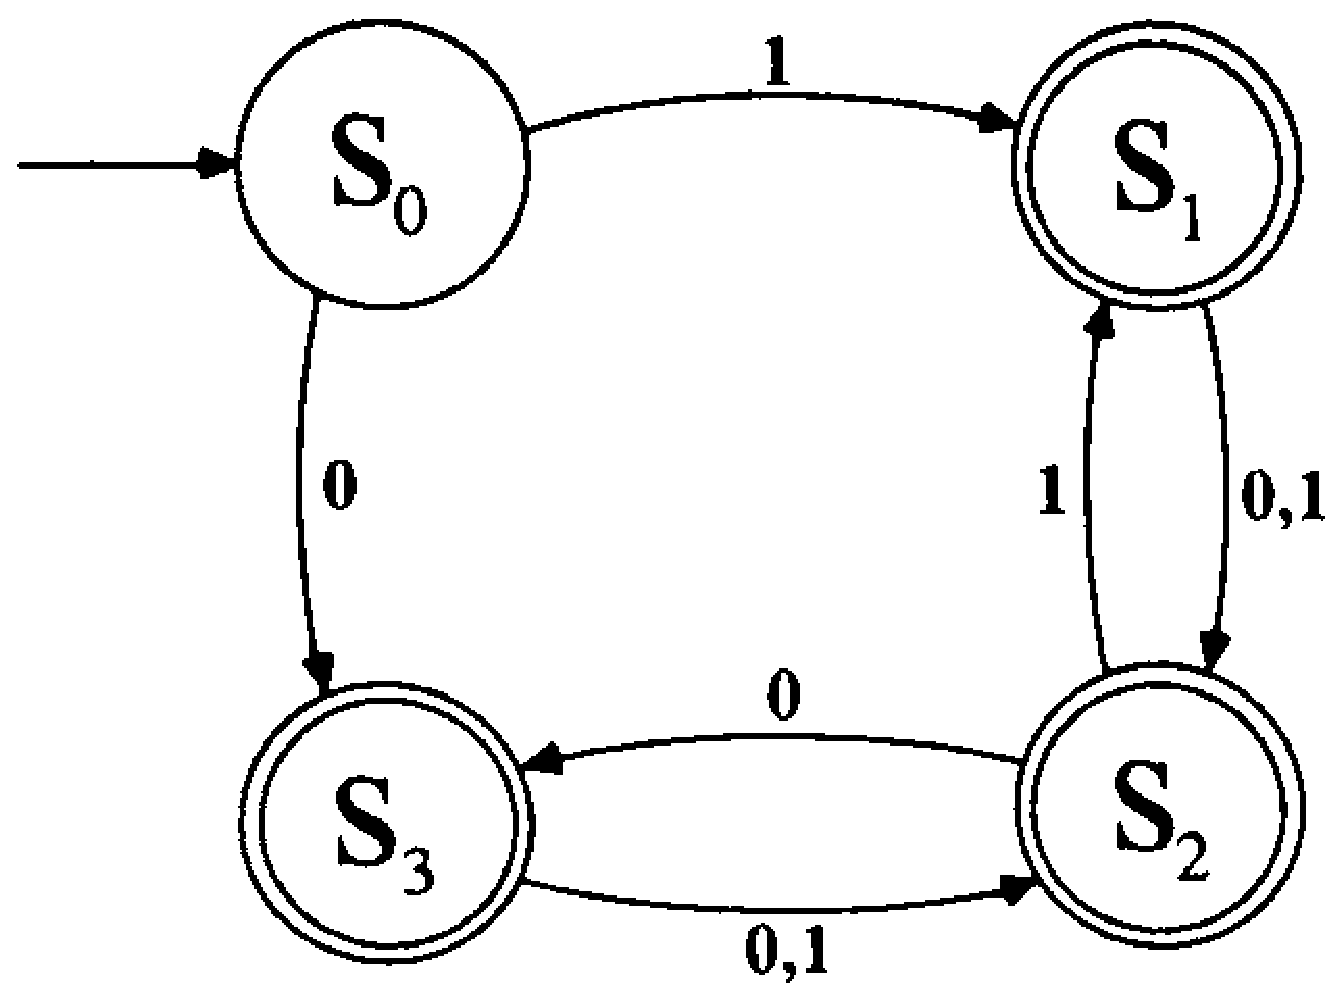
\epsfig{figure=ToFAfigures/fig2-3.eps,width=2.5in}}
\caption{The DFA $N$ discussed in Example 2.6}\label{fig-2.3}
\end{figure}

Let $L$ be the following FAD language: $L=\Sigma^* - \{\lambda\} = \Sigma^+$.
There are many finite automata that accept $L$, one of which is the DFA given in
Figure \ref{fig-2.3}. This four-state machine gives rise to a four-equivalence class right
congruence as described in (1) $\Rightarrow$ (2), where
\begin{center}\begin{tabular}{rclcl}
$[\lambda]_{R^N}$ & $=$ & $I(N,s_0)$ & $=$ & $\{\lambda\}$, since $\lambda$ is
	the only string that ends up at $s_0$ \\
$[\pmb{1}]_{R^N}$ & $=$ & $I(N,s_1)$ & $=$ & $\{y|\ |y|$ is odd, and $y$ ends
	with a $\pmb{1}\} = \{z\ |\DBAR(s_0,z) = s_1\}$ \\
$[\pmb{11}]_{R^N}$ & $=$ & $I(N,s_2)$ & $=$ & $\{y|\ |y|$ is even$\}-\{\lambda\}
	= \{z\ |\DBAR(s_0,z) = s_2\}$ \\
$[\pmb{000}]_{R^N}$ & $=$ & $I(N,s_3)$ & $=$ & $\{y|\ |y|$ is odd, and $y$ ends
	with a $\pmb{0}\} = \{z\ |\DBAR(s_0,z) = s_3\}$
\end{tabular}\end{center}
Note that $L$ is indeed $I(N,s_1) \cup I(N,s_2)  \cup I(N,s_3)$ which is the
union of all the equivalence classes that correspond to final states in $N$, as
required by (2). To illustrate (2) $\Rightarrow$ (3), let $R$ be the equivalence
relation $R^N$ defined above, let $L$ again be $\Sigma^+$, and note that (2) is
satisfied: $L=[\pmb{1}]_R \cup [\pmb{11}]_R \cup [\pmb{000}]_R$, the union of
3 of the equivalence classes of a right congruence of rank 4 (which is finite).

As in the proof of (2) $\Rightarrow$ (3), $R_L$ is refined by $R$, but in this
case $R$ and $R_L$ are not equal. All the relations from $R$ still hold, such as
$\pmb{11}\ R\ \pmb{1111}$, so $\pmb{11}\ R_L\ \pmb{1111}$; $\pmb{0}\ R\ 
\pmb{000}$, and thus $\pmb{0}\ R_L\ \pmb{000}$, and so forth. It can also be
shown that $\pmb{11}\ R_L\ \pmb{000}$, even though $\pmb{11}$ and $\pmb{000}$
were not related by $R$ (apply the definition of $R_L$ to convince yourself of
this). Thus, everything in $[\pmb{11}]_R$ is related by $R_L$ to everything in
$[\pmb{000}]_R$; that is, all the strings belong to the same equivalence class
\emph{of} $R_L$, even though they formed separate equivalence classes \emph{in}
$R$. It may at first appear strange, but the fact that there are \emph{more} relations
in $R_L$ means that there are \emph{fewer} equivalence classes in $R_L$ than in
$R$. Indeed, $R_L$ has only two equivalence classes, $\{\lambda\}$ and $L$. In
this case, three equivalence classes of $R$ collapse to form one large
equivalence class of $R_L$. Thus $\{\lambda\}=[\lambda]_{R_L}=[\lambda]_R$ and
$L=[\pmb{11}]_{R_L}=[\pmb{1}]_R \cup [\pmb{11}]_R \cup [\pmb{000}]_R$ and, as we
were assured by (2) $\Rightarrow$ (3), $R$ refines $R_L$.

To illustrate (3) $\Rightarrow$ (1), let's continue to use the $L$ and $R_L$
given above. Since $R_L$ is of rank 2, we are assured of finding a two-state
machine that will accept $L$. $A_{R_L}$ in this case would take the form of the
automaton $P$ displayed in Figure \ref{fig-2.4}. In this DFA, for example,
$\delta([\pmb{11}]_{R_L},\pmb{0})=[\pmb{110}]_{R_L}=[\pmb{11}]_{R_L}$, and
$[\lambda]_{R_L}$ is the start state. $[\pmb{11}]_{R_L}$ is a final state since
$\pmb{11} \in L$. Verify that this machine accepts all words except $\lambda$;
that is, $L(A_{R_L}) = L$.

\subsection*{Example 2.7}

% Figure 2.4
\begin{figure}
\centerline{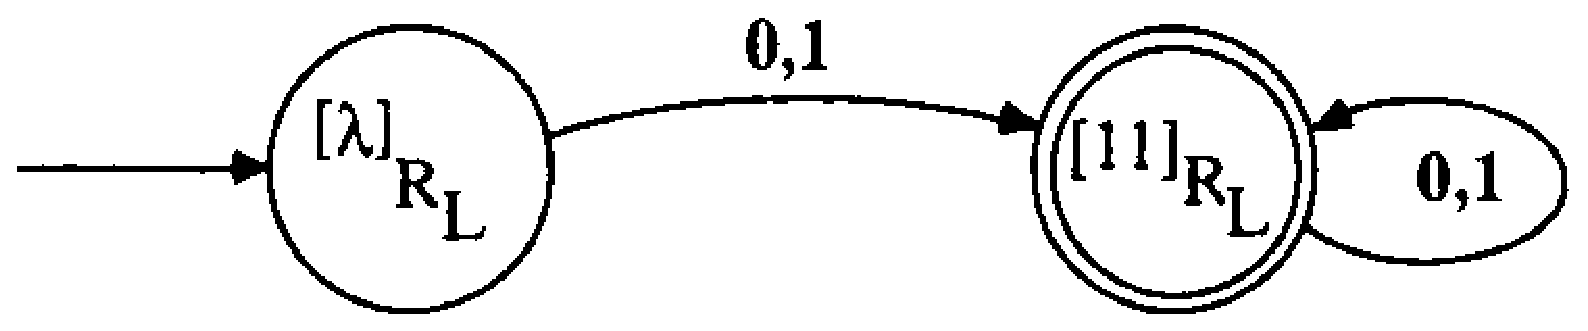
\epsfig{figure=ToFAfigures/fig2-4.eps,width=3.0in}}
\caption{The DFA $P$ discussed in Example 2.6}\label{fig-2.4}
\end{figure}

Assume $Q$ is defined to be the right congruence $R$ given in Example 2.6, and
$L$ is again $\Sigma^+$, which is the union of three of the equivalence classes
of $Q:\ [\pmb{1}]_Q,\ [\pmb{11}]_Q$, and $[\pmb{000}]_Q$. The automaton $A_Q$ is
given in Figure \ref{fig-2.5}.

% Figure 2.5
\begin{figure}
\centerline{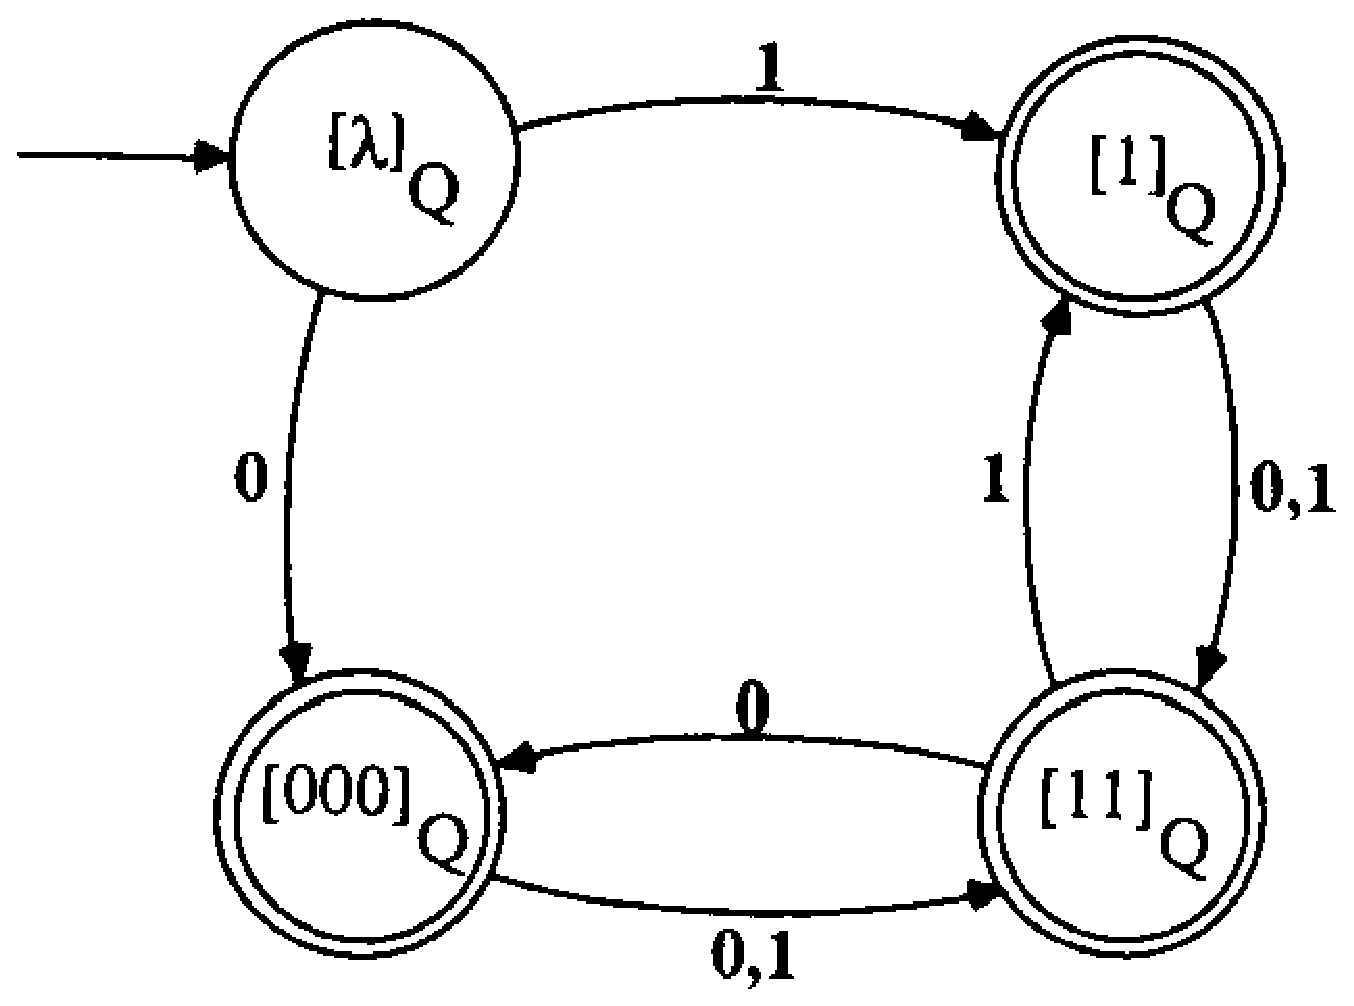
\epsfig{figure=ToFAfigures/fig2-5.eps,width=2.5in}}
\caption{The automaton discussed in Example 2.7}\label{fig-2.5}
\end{figure}

If we were instead to begin with the same language $L$, but use the two-state
machine $P$ at the end of Example 2.6 to represent $L$, we would find that $L$
would consist of only one equivalence class, $R^P$ would have only two
equivalence classes, and $R^P$ would in this case be the same as $R_L$ (see the
exercises). $R^P$ turns out to be as simple as $R_L$ because the machine we
started with was as ``simple'' as we could get and still represent $L$. In
Chapter \ref{ch-3} we will characterize the idea of a machine being ``as simple as
possible,'' that is, \emph{\Index{minimal}}.

The two machines given in Example 2.6 accept the same language. It will be
convenient to formalize this notion of distinct machines ``performing the same
task,'' and we therefore make the following definition.

% Definition 2.6
\begin{dfn}\label{dfn-2.6}\index{equivalent!DFAs}
Two DFAs $A$ and $B$ are \emph{equivalent} iff $L(A) = L(B)$.
\end{dfn}

\subsection*{Example 2.8}

The DFAs $N$ from Example 2.6 and $A_Q$ from Example 2.7 are equivalent since
$L(N) = \Sigma^+ = L(A_Q)$ .

% Definition 2.7
\begin{dfn}\label{dfn-2.7}
A DFA $A=\langle\Sigma,S_A,s_{0_A},\delta_A,F_A\rangle$ is \emph{\Index{minimal}}
iff for every DFA $B=\langle\Sigma,S_B,s_{0_B},\delta_B,F_B\rangle$ for which
$L(A) = L(B),\ |S_A| \leq |S_B|$.
\end{dfn}

An automaton is therefore minimal if no equivalent machine has fewer states.

\subsection*{Example 2.9}

The DFA $N$ from Example 2.6 is clearly not minimal since the automaton $P$
from Example 2.6 is equivalent and has fewer states than $N$. The techniques
from Chapter \ref{ch-3} can be used to verify that the automaton $P$ from Example 2.6
is minimal. More importantly, minimization techniques will be explored in
Chapter \ref{ch-3} that will allow an optimal machine (like this $P$) to be produced
from an inefficient automaton (like $N$).

\section{Pumping Lemmas}\label{sec-2.3}

As you have probably noticed by now, finding $R_L$ and counting the equivalence
classes is not a very practical way of verifying that a suspected language
cannot be defined by a finite automaton. It would be nice to have a better way
to determine if a given language is unwieldy. The \emph{\Index{pumping lemma}}
will supply us with such a technique. It is based on the observation that if
your automaton processes a ``long enough'' word it must eventually visit (at
least) one state more than once.

Let $A=\langle\Sigma,S,s_0,\delta,F\rangle$, and consider starting at some state
$s$ and processing a word $x$ of length 5. We will pass through state $s$ and
perhaps five other states, although these states may not all be distinct if we
visit some of them repeatedly while processing the five letters in $x$; thus the
total will be six states (or less). Note that if $A$ has 10 states $(\|S\|=10)$
and $|x| = 12$ we cannot go to 13 \emph{different} states while processing $x$;
(at least) one state must be visited more than once.

% Figure 2.6
\begin{figure}
\centerline{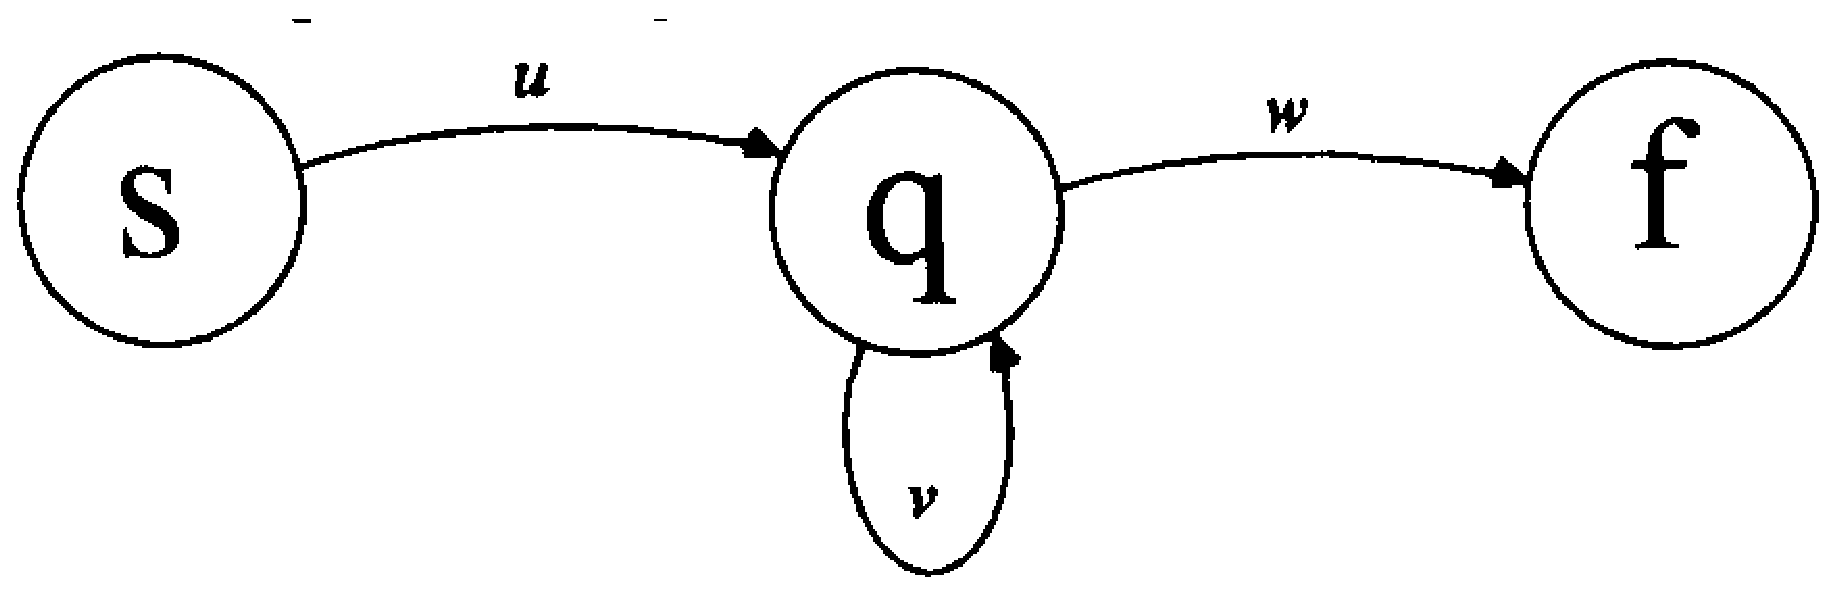
\epsfig{figure=ToFAfigures/fig2-6.eps,width=4.0in}}
\caption{A path with a loop}\label{fig-2.6}
\end{figure}

In general, if $n=\|S\|$, then any string $x$ whose length is equal to or
greater than $n$ must pass through some state $q$ twice while being processed by
$A$, as shown in Figure \ref{fig-2.6}. Here the arrows are meant to represent the path
taken while processing \emph{several} letters, and the intermediate states are not
shown. The strings $u$, $v$, and $w$ are defined as
\begin{center}\begin{tabular}{l}
$u$ = first few letters of $x$ that take us to the state $q$ \\
$v$ = next few letters of $x$ that will again take us back to $q$ \\
$w$ = rest of the string $x$
\end{tabular}\end{center}
Then, with $x = uvw$, we have $\DBAR(s,u) = q,\ \DBAR(s,uv) = q$, and in fact
$\DBAR(q,v) = q$. Also, $\DBAR(s,x) = \DBAR(s,uvw) =$ $f$ and $\DBAR(q,w)= f$, as
is clear from the diagram. Now consider the string $uw$, that is, the string $x$
with the $v$ part ``removed'':
\begin{center}\begin{tabular}{rcl}
$\DBAR(s,uw)$ & $=$ & $\DBAR(\DBAR(s,u),w)\qquad\text{(why?)}$ \\
& $=$ & $\DBAR(q,w)$ \\
& $=$ & $f$
\end{tabular}\end{center}
That is, the string $uw$ winds up in the same place $uvw$ does; this is
illustrated in Figure \ref{fig-2.7}a. Note that a similar thing happens if $uv^2 w$ is
processed:
\begin{center}\begin{tabular}{rcl}
$\DBAR(s,uvvw)$ & $=$ & $\DBAR(\DBAR(s,u),vvw)$ \\
& $=$ & $\DBAR(q,vvw)$ \\
& $=$ & $\DBAR(\DBAR(q,v),vw)$ \\
& $=$ & $\DBAR(q,vw)$ \\
& $=$ & $\DBAR(\DBAR(q,v),w)$ \\
& $=$ & $\DBAR(q,w)$ \\
& $=$ & $f$
\end{tabular}\end{center}
This behavior is illustrated in Figure \ref{fig-2.7}b.

% Figure 2.7
\begin{figure}
\centerline{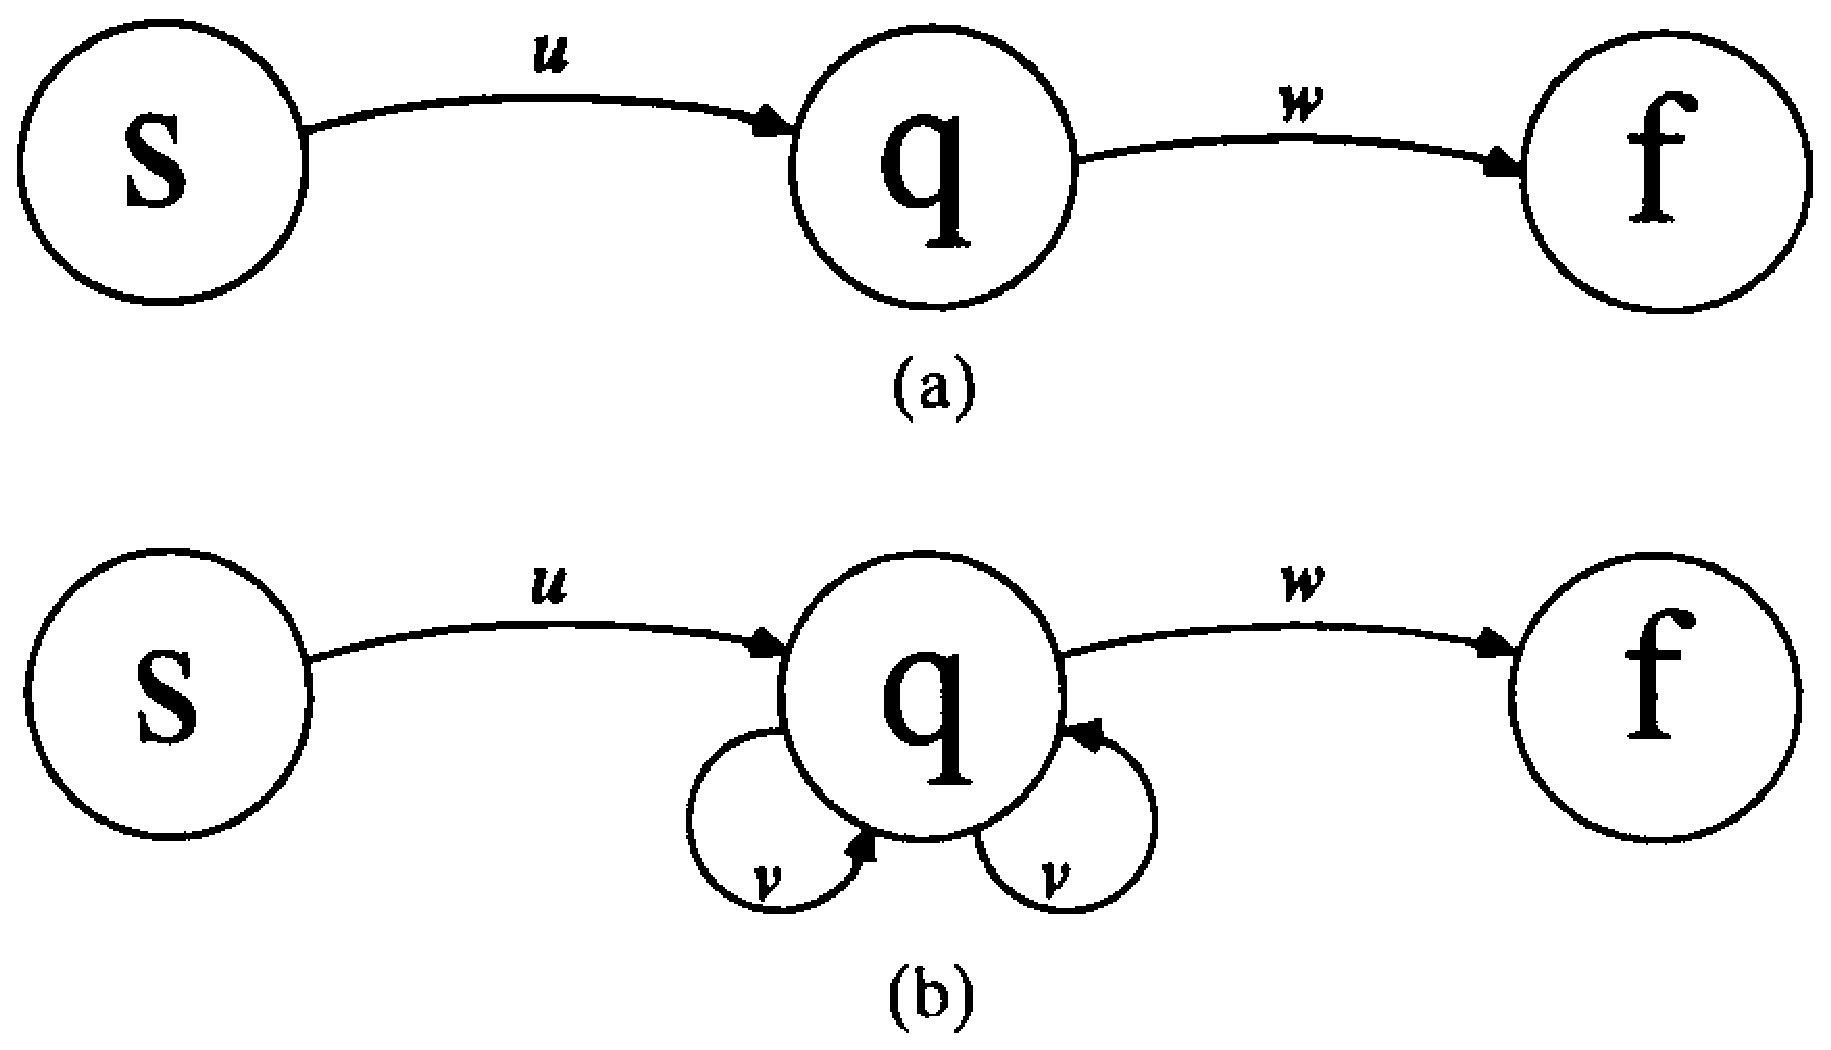
\epsfig{figure=ToFAfigures/fig2-7.eps,width=4.0in}}
\caption{(a) The path that bypasses the loop (b) The path that traverses the
loop twice}\label{fig-2.7}
\end{figure}

In general, it can be proved by induction that $(\forall i \in \NN)(\DBAR(s,
uv^i\!w)=\text{f}=\DBAR(s,uvw))$. Notice that we do reach $q$ two \emph{distinct} times,
which implies that the string $v$ contains at least one letter; that is,
$|v| \geq 1$. Also, after the first $n$ letters of $x$, we must have already
repeated a state, and thus some state $q$ can be found such that $|uv| \leq n$.
If $s$ happens to be the start state $s_0$ and $f$ is a final state, we have
now shown that: If $A=\langle\Sigma,S,s_0,\delta,F\rangle$, where $\|S\| = n$,
then, given any string $x=\pmb{a}_1\pmb{a}_2\pmb{a}_3 \ldots \pmb{a}_m$, where
$m \geq n$ and $\DBAR(s_0,x)= f \in F$ [which implies $x \in L(A)$], the states
$\DBAR(s_0,\lambda),\DBAR(s_0,\pmb{a}_1),\DBAR(s_0,\pmb{a}_1\pmb{a}_2),
\DBAR(s_0,\pmb{a}_1\pmb{a}_2\pmb{a}_3), \ldots ,\DBAR(s_0,\pmb{a}_1\pmb{a}_2
\ldots \pmb{a}_n)$ cannot all be distinct, and so $x$ can be broken up into
strings $u$, $v$, and $w$ such that
\begin{center}\begin{tabular}{rcl}
$x$ & $=$ & $uvw$ \\
$|uv|$ & $\leq$ & $n$ \\
$|v|$ & $\geq$ & $1$
\end{tabular}\end{center}
and $(\forall i \in \NN)(\DBAR(s_0,uv^i\!w)=$f$)$, that is, $(\forall i \in \NN)
(uv^i\!w \in L(A))$. In other words, given any ``long'' string in $L(A)$, there is
a part of the string that can be ``pumped'' to produce even longer strings in
$L(A)$.

Thus, if $L$ is FAD, there exists an automaton (with a finite number $n$ of
states), and thus for some $n\in\NN$, the above statement should hold. We have
just proved what is generally known as the \emph{pumping lemma}, which we now
state formally.

% Theorem 2.3: The Pumping Lemma
\begin{thm}\label{thm-2.3}
{\bf The Pumping Lemma.} Let $L$ be an FAD language over $\Sigma^*$. Then
$(\exists n \in \NN)(\forall x \in L \ni |x| \geq n)(\exists u,v,w \in
\Sigma^*) \ni$
\begin{center}\begin{tabular}{rcl}
$x$ & $=$ & $uvw$ \\
$|uv|$ & $\leq$ & $n$ \\
$|v|$ & $\geq$ & $1$
\end{tabular}\end{center}
and
\[ (\forall i \in \NN)(uv^i\!w \in L). \]

\emph{Proof.} Given above.
\end{thm}

\subsection*{Example 2.10}

Let $E$ be the set of all even-length words over $\{\pmb{a},\pmb{b}\}^*$. There is
a two-state machine that accepts $E$, so $E$ is FAD, and the pumping lemma
applies if $n$ is, say, 5. Then $\forall x \ni |x| > 5$, if $x = 
\pmb{a}_1\pmb{a}_2\pmb{a}_3\ldots\pmb{a}_j \in E$ (that is, $j$ is even), we can
choose $u=\lambda,\ v=\pmb{a}_1\pmb{a}_2$, and $w=\pmb{a}_3\pmb{a}_4\ldots
\pmb{a}_j$. Note that $|uv|= 2 \leq 5$, $|v| = 2 \geq 1$, and $|uv^iw|=j+2(i-1)$,
which is even, and so $(\forall i \in \NN)(uv^iw \in E)$.

If Example 2.10 does not appear truly exciting, there is good reason: The
pumping lemma is generally not applied to FAD languages! (\emph{Note:} We \emph{will}
see an application later.) The pumping lemma is often applied to show languages
are \emph{not} FAD (by proving that the language does not satisfy the pumping lemma).
Note that the contrapositive of Theorem \ref{thm-2.3} is:

% Theorem 2.4
\begin{thm}\label{thm-2.4}
Let $L$ be a language over $\Sigma^*$. {\bf If} \\
$(\forall n \in \NN)(\exists x \in L \ni |x| \geq n)(\forall u,v,w \in
\Sigma^* \ni x = uvw,|uv| \leq n, |v| \geq 1)(\exists i \in \NN \ni uv^i\!w
\notin L)$, \\
{\bf then} $L$ is not FAD.

\emph{Proof.} See the exercises.
\end{thm}

\subsection*{Example 2.11}

Consider $L_4=\{y \in \{\pmb{0},\pmb{1}\}^*|\ |y|_{\pmb{0}} = |y|_{\pmb{1}}\}$. We will
use Theorem \ref{thm-2.4} to show $L_4$ is not FAD: Let $n$ be given, and choose $x =
\pmb{0}^n \pmb{1}^n$. Then $x \in L_4$, since $|x|_{\pmb{0}} = n = |x|_{\pmb{1}}$. It should be
observed that $x$ must be dependent on $n$, and we have \emph{no} control over
$n$ (in particular, $n$ cannot be replaced by some constant; similarly, while
$i$ may be chosen to be a convenient fixed constant, a proof that covers all possible
combinations of $u$, $v$, and $w$ must be given).

Note that this choice of $x$ is ``long enough'' in that $|x| = 2n \geq n$, as
required by Theorem \ref{thm-2.4}. For \emph{any} combination of $u,\ v,\ w \in \Sigma^*$ such
that $x = uvw,\ |uv| \leq n,\ |v| \geq 1$, we hope to find a value for $i$ such
that $uv^iw \notin L_4$. Since $|uv| \leq n$ and the first $n$ letters of $x$ are
all zeros, this narrows down the choices for $u,\ v$, and $w$. They must be of
the form $u = \pmb{0}^j$ and $v = \pmb{0}^k$ (since $|uv| \leq n$ and $x$ starts
with $n$ zeros), and $w$ must be the ``rest of the string'' and look something
like $w=\pmb{0}^m \pmb{1}^n$. The constraints on $u,\ v$, and $w$ imply that
$j + k \leq n,\ k \geq 1$, and $j + k + m = n$. If $i = 2$, we have that
$uv^2w = \pmb{0}^{n+k} \pmb{1}^n \notin L_4$ (why?). Thus, by Theorem \ref{thm-2.4}, $L_4$ is not FAD
[or, alternately, because the conclusion of the pumping lemma (Theorem \ref{thm-2.3}) does
\emph{not} hold, $L_4$ cannot be FAD].

It is instructive to endeavor to build a DFA that attempts to recognize the
language $L_4$. As you begin to see what such a machine must look like, it
will become clear that no matter how many states you add (that is, no matter how
large $n$ becomes) there will always be some strings (``long'' strings) that
would require even more states. Your construction may also suggest what the
equivalence classes of $R_{L_4}$ must look like (see the exercises). How many
equivalence classes are there? (You should be able to answer this last question
without referring to any constructions.)

A similar argument can be made to show that no DFA can recognize the set of all
fully parenthesized infix expressions (see the exercises). Matching parentheses,
like matching $\pmb{0}$s and $\pmb{1}$s in the last example, requires unlimited
storage. We have seen that DFAs are adequate vehicles for pattern matching and
token identification, but a more complex model is clearly needed to implement
functions like the parsing of arithmetic expressions. \emph{Pushdown automata},\index{pushdown automaton} discussed in Chapter \ref{ch-10}, augment the finite memory with an unbounded
stack, allowing more complex languages to be recognized.

Intuitively, we would not expect \emph{finite}-state machines to be able to
differentiate between arbitrarily long integers. While \emph{modular}
arithmetic, which only differentiates between a finite number of remainders,
should be representable by finite automata, unrestricted arithmetic is likely to
be impossible. For example, $\{\pmb{a}^i\pmb{b}^j\pmb{c}^k\ |\ i,j,k \in \NN$ and
$i + j = k\}$ cannot be recognized by any DFA, while the language
$\{\pmb{a}^i\pmb{b}^j\pmb{c}^k\ |\ i,j,k \in \NN$ and $i + j \equiv k \bmod{3}\}$ is
FAD. Checking whether two numbers are relatively prime is likewise too difficult
for a DFA, as shown by the proof in the following example.

\subsection*{Example 2.12}

Consider $L=\{\pmb{a}^i\pmb{b}^j\ |\ i,j \in \NN$ and $i$ and $j$ are relatively
prime$\}$. We will use Theorem \ref{thm-2.4} to show $L$ is not FAD: Let $n$ be given, and
choose a prime $p$ larger than $n + 1$ (we can be assured such a $p$ exists
since there are an infinite number of primes). Let $x=\pmb{a}^p\pmb{b}^{(p-1)!}$.
Since $p$ has no factors other than $1$ and $p$, it has no nontrivial factor in
common with $(p-1) \cdot (p-2) \cdot \ldots \cdot 3 \cdot 2 \cdot 1$, and so $p$
and $(p-1)!$ are relatively prime, which guarantees that $x \in L$. The length
of $x$ is clearly greater than $n$, so Theorem \ref{thm-2.3} should apply, which implies
that there must exist a combination $u,v,w \in \Sigma^*$ such that $x = uvw,
|uv| \leq n, |v| \geq 1$; we hope to find a value for $i$ such that $uv^iw \in L$.
Since $|uv| \leq n$ and the first $n$ letters of $x$ are all $\pmb{a}$s, there
must exist integers $j,\ k$, and $m$ for which $u=\pmb{a}^j$ and $v=\pmb{a}^k$,
and $w$ must be the ``rest of the string''; that is, $w=\pmb{a}^m
\pmb{b}^{(p-1)!}$. The constraints on $u,\ v$, and $w$ imply that $j + k \leq n$,
$k \geq 1$, and $j + k + m = p$. If $i = 0$, we have that $uv^{0} w =
\pmb{a}^{p-k}\pmb{b}^{(p-1)!}$. But $p-k$ is a number between $p-1$ and $p-n$
and hence must match one of the nontrivial factors in $(p-1)!$, which means that
$uv^{0} w \notin L$ (why?). Therefore, Theorem \ref{thm-2.3} has been violated, so $L$
could not have been FAD.

The details of the basic argument used to prove the pumping lemma can be varied
to produce other theorems of a similar nature: for example, when processing $x$,
there must be a state $q'$ repeated within the last $n$ letters. This gives rise
to the following variation of the pumping lemma.

% Theorem 2.5
\begin{thm}\label{thm-2.5}
Let $L$ be a FAD language over $\Sigma^*$. Then
\[ (\exists n \in \NN)(\forall x \in L \ni |x| \geq n)(\exists u,v,w \in
	\Sigma^*) \ni \]
\begin{center}\begin{tabular}{rcl}
$x$ & $=$ & $uvw$ \\
$|vw|$ & $\leq$ & $n$, \\
$|v|$ & $\geq$ & $1$ \\
\end{tabular}\end{center}
and
\[ (\forall i \in \NN)(uv^iw \in L) \]

\emph{Proof.} See the exercises.
\end{thm}

The new condition $|vw| \leq n$ reflects the constraint that some state must be
repeated within the last $n$ letters. The contrapositive of Theorem \ref{thm-2.5} can be
useful in demonstrating that certain languages are not FAD. By repeating our
original reasoning while assuming the string $x$ takes us to a \emph{non}final state,
we obtain yet another variation.

% Theorem 2.6
\begin{thm}\label{thm-2.6}
Let $L$ be a FAD language over $\Sigma^*$. Then
\[ (\exists n \in \NN)(\forall x \notin L \ni |x| \geq n)(\exists u,v,w \in
	\Sigma^*) \ni \]
\begin{center}\begin{tabular}{rcl}
$x$ & $=$ & $uvw$ \\
$|uv|$ & $\leq$ & $n$ \\
$|v|$ & $\geq$ & $1$ \\
\end{tabular}\end{center}
and
\[ (\forall i \in \NN)(uv^iw \notin L) \]

\emph{Proof.} See the exercises.
\end{thm}

Notice that Theorem \ref{thm-2.6} guarantees that if one ``long'' string is
{\em not} in the
language then there is an entire sequence of strings that cannot be in the
language. There are some examples of languages in the exercises where Theorem
\ref{thm-2.4} is hard to apply, but where Theorem \ref{thm-2.5} (or Theorem \ref{thm-2.6}) is appropriate.

When $i = 0$, the pumping lemma states that given a ``long'' string ($uvw$) in
$L$ there is a shorter string ($uw$) that is also in $L$. If this new string is
still of length greater than $n$, the pumping lemma can be reapplied to find a
still shorter string, and so on. This technique is the basis for proving the
following theorem.

% Theorem 2.7
\begin{thm}\label{thm-2.7}
Let $M$ be an $n$-state DFA accepting $L$. Then
\[ (\forall x \in L \ni x = \pmb{a}_1\pmb{a}_2 \ldots \pmb{a}_m,\text{ and }m
	\geq n)(\exists\text{ an increasing sequence }i_1,i_2, \ldots ,i_j) \]
for which $\pmb{a}_{i_1}\pmb{a}_{i_2} \ldots \pmb{a}_{i_j} \in L$, and $j < n$.

\emph{Proof.} See the exercises.
\end{thm}

Note that $\pmb{a}_{i_1}\pmb{a}_{i_2} \ldots \pmb{a}_{i_j}$ represents a string
formed by ``removing'' letters from perhaps several places in $x$, and that this
new string has length less than $n$. Theorem \ref{thm-2.7} can be applied in areas that do
not initially seem to relate to DFAs. Consider an arbitrary right congruence $R$
of (finite) rank $n$. It can be shown that each equivalence class of $R$ is
guaranteed to contain a representative of length less than $n$. For example,
consider the relation $R$ given by
\begin{center}\begin{tabular}{rcl}
$[\lambda]_R$ & $=$ & $\{\lambda\}$ \\
$[\pmb{11111}]_R$ & $=$ & $\{y\ |\ \ |y|\text{ is odd, and $y$ ends with a }
	\pmb{1}\}$ \\
$[\pmb{0101}]_R$ & $=$ & $\{y\ |\ \  |y|\text{ is even and }|y| > 0\}$ \\
$[\pmb{00000}]_R$ & $=$ & $\{y\ |\ \  |y|\text{ is odd, and $y$ ends with a }
	\pmb{0}\}$
\end{tabular}\end{center}
In this relation, $rk(R) = 4$, and appropriate representatives of length less
than 4 are $\lambda,\ \pmb{1},\ \pmb{11}$, and $\pmb{100}$, respectively. That
is, $[\lambda]_R = [\lambda]_R,\ [\pmb{1}]_R = [\pmb{11111}]_R,\ [\pmb{11}]_R
= [\pmb{0101}]_R$, and $[\pmb{100}]_R = [\pmb{00000}]_R$. By constructing a DFA
based on the right congruence $R$, Theorem \ref{thm-2.7} can be used to prove that every
equivalence class of $R$ has a ``short'' representative (see the exercises).

We have seen that deterministic finite automata are limited in their cognitive
powers, that is, there are languages that are too complex to be recognized by
DFAs. When only a finite set of previous histories can be distinguished, the
resulting languages must have a certain repetitious nature. Allowing automata to
instead have an infinite number of states is uninteresting for several reasons.
On the practical side, it would be inconvenient (to say the least) to physically
construct such a machine. Infinite automata are also of little theoretical
interest as they do not distinguish between simple and complex languages: {\em any}
language can be accepted by the infinite analog of a DFA. With an infinite
number of states available, the state transition diagrams can look like trees,
with a unique state corresponding to each word in $\Sigma^*$. The states
corresponding to desired words can simply be made final states.

More reasonable enhancements to automata will be explored later. Non-determinism
will be presented in Chapter \ref{ch-4}, and machines with extended capabilities will be
defined and investigated in Chapters \ref{ch-10} and \ref{ch-11}.

\section*{Exercises}

\begin{enumerate}[{2.}1.]
\item Let $\Sigma=\{\pmb{a},\pmb{b},\pmb{c}\}$. Show that the relation $\Psi
\subseteq \Sigma^* \times \Sigma^*$ defined by
\[ x\ \Psi\ y \Leftrightarrow |x|-|y|\text{ is odd} \]
is \emph{not} a right congruence. (Is it an equivalence relation?)

\item Let $\Sigma=\{\pmb{a},\pmb{b},\pmb{c}\}$. Consider the relation $Q
\subseteq \Sigma^* \times \Sigma^*$ defined by
\[ x\ Q\ y \Leftrightarrow |x|_{\pmb{a}} - |y|_{\pmb{a}} \equiv 0 \bmod{3} \]
\begin{enumerate}
\item Show that $Q$ is an equivalence relation.
\item Assume that part (a) is true, and show that $Q$ is a right congruence.
\end{enumerate}

\item Let $\Sigma=\{\pmb{a},\pmb{b},\pmb{c}\}$. Find all languages $L$ such that
$rk(R_L) = 1$. Justify your conclusions.

\item Let $P \subseteq \{\pmb{0},\pmb{1}\}^* \times \{\pmb{0},\pmb{1}\}^*$ be
the equivalence relation with the following equivalence classes:
\begin{center}\begin{tabular}{rcl}
$[\lambda]_P$ & $=$ & $\{\lambda\} = \{\pmb{0},\pmb{1}\}^0$ \\
$[\pmb{1}]_P$ & $=$ & $\{\pmb{0},\pmb{1}\} = \{\pmb{0},\pmb{1}\}^1$ \\
$[\pmb{00}]_P$ & $=$ & $\{\pmb{0},\pmb{1}\}^2 \cup \{\pmb{0},\pmb{1}\}^3 \cup
	\{\pmb{0},\pmb{1}\}^4 \cup \{\pmb{0},\pmb{1}\}^5 \cup \ldots$
\end{tabular}\end{center}
Show that $P$ is a right congruence.

\item For the relation $P$ defined in Exercise 2.4, find all languages $L \ni
R_L = P$.

\item For the relation $Q$ defined in Exercise 2.2, find all languages $L \ni
R_L = Q$.

% NOTE: Having trouble getting the spacing on the \not portion of the !Q
% operator
\item Let $\Sigma=\{\pmb{a},\pmb{b}\}$. Define the relation $Q$ by $\lambda Q
\lambda$, and $(\forall x \not= \lambda)(\lambda \not\!\! Q x)$, and
\[ (\forall x \not= \lambda)(\forall y \not= \lambda )[x\ Q\ y \Leftrightarrow
	(|x|\text{ is even }\wedge |y|\text{ is even})\vee(|x|\text{ is odd }
	\wedge |y|\text{ is odd})], \]
which implies that
\[ (\forall x \not= \lambda)(\forall y \not= \lambda)[x \not\!\! Q\ y
	\Leftrightarrow (|x|\text{ is even }\wedge |y|\text{ is odd})\vee(|x|
	\text{ is odd} \wedge |y|\text{ is even})]. \]
\begin{enumerate}
\item Show that $Q$ is a right congruence. and list the equivalence classes.
\item Define $L=[\lambda]_Q \cup [\pmb{aa}]_Q$. Find a simple description for
$L$, and list the equivalence classes of $R_L$. (Note that $Q$ does refine
$R_L$.)
\item Draw a machine with states corresponding to the equivalence classes of
$Q$. Arrange the final states so that the machine accepts $L$ (that is, find
$A_Q$).
\item Draw $A_{R_L}$.
\item Consider the machine in part (c) above ($A_Q$). Does it look like
$A_{R_L}$? Can you rearrange the final states in $A_Q$ (producing a new language
$K$) so that $A_{R_K}$ looks like your new $A_Q$? Illustrate.
\item Consider all eight languages found by taking unions of equivalence classes
from $Q$, and see which ones would satisfy the criteria of part (e).
\end{enumerate}

\item Let $\Sigma=\{\pmb{a}\}$. Let $I$ be the identity relation on $\Sigma^*$.
\begin{enumerate}
\item Show that $I$ is a right congruence.
\item What do the equivalence classes of $I$ look like?
\end{enumerate}

\item Let $\Sigma=\{\pmb{a}\}$, and let $I$ be the identity relation on
$\Sigma^*$. Let $L=\{\lambda\} \cup \{\pmb{a}\} \cup \{\pmb{aa}\}$, which is
the union of three of the equivalence classes of $I$. $I$ has infinite rank.
Does Nerode's theorem imply that $L$ is not FAD? Explain.

\item Define a machine $M=\langle\Sigma,S_M,s_0,\delta,F_M\rangle$ for which
$rk(R_{L(M)}) \not= \|S_M\|$.

\item Carefully show that $F_{R_L}$ is a well-defined set; that is, show that
the rule that assigns equivalence classes to $F_{R_L}$ is unambiguous.

\item Carefully show that $\delta_{R_L}$ is well-defined, that is, that
$\delta_{R_L}$ is a \emph{function}.

\item Use induction to show that $(\forall x \in \Sigma^*)(\forall y \in
\Sigma^*)(\DBAR_{R_L}([x]_{R_L},y) = [xy]_{R_L})$.

\item Consider the automaton $P$ derived in Example 2.6, find $R^P$ and notice
that $R^P = R_L$.

\item Find $R^A$ for each machine $A$ you built in the exercises of Chapter \ref{ch-1};
compare $R^A$ to $R_{L(A)}$.

\item Prove by induction that, for the strings defined in the discussion of
the pumping lemma,\\$(\forall i\in\NN)(\DBAR(s,uv^iw) 	= f =\DBAR(s,uvw))$.

\item Prove Theorem \ref{thm-2.1}.

\item \begin{enumerate}
\item Find a language that gives rise to the relation $I$ defined in Exercise
2.8.
\item Could such a language be FAD? Explain.
\end{enumerate}

\item Starting with Theorem \ref{thm-2.3} as a given hypothesis, prove Theorem \ref{thm-2.4}.

\item Prove Theorem \ref{thm-2.5} by constructing an argument similar to that given for
Theorem \ref{thm-2.3}.

\item Prove Theorem \ref{thm-2.6} by constructing an argument similar to that given for
Theorem \ref{thm-2.3}.

\item Prove Theorem \ref{thm-2.7}.

\item Let $L=\{x \in\{\pmb{a},\pmb{b}\}^*\ |\ \ |x|_{\pmb{a}} < |x|_{\pmb{b}}\}$.
Show $L$ is not FAD.

\item Let $G=\{x \in\{\pmb{a},\pmb{b}\}^*\ |\ \ |x|_{\pmb{a}} \geq |x|_{\pmb{b}}\}$.
Show $G$ is not FAD.

\item Let $P=\{y \in \{\pmb{d}\}^*\ |\ \exists\text{ prime }p \ni y = \pmb{d}^p\} =
\{\pmb{dd},\pmb{ddd},\pmb{ddddd},\pmb{d}^7,\pmb{d}^{11},\pmb{d}^{13}\ldots\}$.
Prove that $P$ is not FAD.

\item Let $\Gamma=\{x \in \{\pmb{0},\pmb{1},\pmb{2}\}^*\ |\ \exists w\in\{\pmb{0},
\pmb{1}\}^* \ni x = w \cdot \pmb{2} \cdot w\} = \{\pmb{2},\pmb{121},\pmb{020},
\pmb{11211},\pmb{10210},\ldots\}$. Prove that $\Gamma$ is not FAD.

\item Let $\Psi=\{x \in \{\pmb{0},\pmb{1}\}^*\ |\ \exists w \in \{\pmb{0},
\pmb{1}\}^* \ni x = w \cdot w\} = \{\lambda,\pmb{00},\pmb{11},\pmb{0000},
\pmb{1010},\pmb{1111}, \ldots \}$. Prove that $\Psi$ is not FAD.

\item Define the reverse of a string $w$ as follows: If $w=\pmb{a}_1\pmb{a}_2
\pmb{a}_3\pmb{a}_4 \ldots \pmb{a}_{n-1}\pmb{a}_n$, then $w^r=\pmb{a}_n
\pmb{a}_{n-1} \ldots \pmb{a}_4\pmb{a}_3\pmb{a}_2\pmb{a}_1$. Let
$K=\{w \in \{\pmb{0},\pmb{1}\}^*\ |\ w = w^r\} = \{\lambda,\pmb{0},\pmb{1},\pmb{00},
\pmb{11},\pmb{000},\pmb{010},\pmb{101},\pmb{111},\pmb{0000},\pmb{0110},\ldots\}$.
Prove $K$ is not FAD.

\item Let $\Phi=\{x \in \{\pmb{a},\pmb{b},\pmb{c}\}^*\ |\ \exists j,k,m \in \NN \ni
x = \pmb{a}^j\pmb{b}^k\pmb{c}^m$, where $j \geq 3$ and $k = m\}$. Prove $\Phi$ is
not FAD. \emph{Hint:} The first version of the pumping lemma is hard to apply
here (why?).

\item Let $C=\{y \in \{\pmb{d}\}^*\ |\ \exists\text{ \emph{non}prime }q \ni y =
\pmb{d}^q\} = \{\lambda,\pmb{d},\pmb{d}^4,\pmb{d}^6,\pmb{d}^8,\pmb{d}^9,
\pmb{d}^{10} \ldots \}$. Show $C$ is not FAD. \emph{Hint:} The first version of
the pumping 	lemma is hard to apply here (why?).

\item Assume $\Sigma=\{\pmb{a},\pmb{b}\}$ and $L$ is a language for which $R_L$
has the following three equivalence classes: $\{\lambda\}$, $\{$all odd-length
words$\}$, $\{$all even-length words except $\lambda\}$.
\begin{enumerate}
\item Why couldn't $L=\{x\ |\ \ |x|\text{ is odd}\}$? (\emph{Hint:} Recompute
$R_{\{x|\ |x|\text{ is odd}\}})$.
\item List the languages $L$ that \emph{could} give rise to this $R_L$.
\end{enumerate}

\item Let $\Sigma=\{\pmb{a},\pmb{b}\}$ and let $\Psi=\{x \in \Sigma^*\ |\ x$ has an
even number of $\pmb{a}$s and ends with (at least) one $\pmb{b}\}$.
Describe $R_{\Psi}$, and draw a machine accepting $\Psi$.

\item Let $\Xi=\{x \in \{\pmb{a}\}^*\ |\ \exists j \in \NN \ni |x| = j^2\} =
\{\lambda,\pmb{a},\pmb{aaaa},\pmb{a}^9,\pmb{a}^{16},\pmb{a}^{25}, \ldots \}$.
Prove that $\Xi$ is not FAD.

\item Let $\Phi=\{x \in \{\pmb{b}\}^*\ |\ \exists j \in \NN \ni |x| = 2^j\} = 
\{\pmb{b},\pmb{bb},\pmb{bbbb},\pmb{b}^8,\pmb{b}^{16},\pmb{b}^{32}, \ldots \}$.
Prove that $\Phi$ is not FAD.

\item Let $\Sigma=\{\pmb{a},\pmb{b}\}$. Assume $R_L$ has the following five
equivalence classes: $\{\lambda\},\ \{\pmb{a}\}, \{\pmb{aa}\},\ \{\pmb{a}^3,
\pmb{a}^4,\pmb{a}^5,\pmb{a}^6, \ldots \},\linebreak\{x\ |\ x$ contains (at least) one
$\pmb{b}\}$. Also assume that $L$ consists of exactly \emph{one} of these equivalence
classes.
\begin{enumerate}
\item Which equivalence class is $L$?
\item List the other languages $L$ that \emph{could} give rise to this $R_L$
(and note that they might consist of several equivalence classes).
\end{enumerate}

\item Let $\Omega=\{y \in \{\pmb{0},\pmb{1}\}^*\ |\ (y$ contains exactly one 
$\pmb{0}) \vee (y$ contains an even number of $\pmb{1}$s$)\}$. Find $R_\Omega$.

\item Let $\Sigma=\{\pmb{a},\pmb{b}\}$ and $L_1=\{x \in \Sigma^*\ |\ \ |x|_{\pmb{a}} 
> |x|_{\pmb{b}}\}$ and $L_2=\{x \in \Sigma^*|\ |x|_{\pmb{a}} < 3\}$. Which of
the following are FAD? Support your answers. \\
$\text{(a) }L_1\hfill\text{(b) }L_2\hfill\text{(c) }L_1 \cap L_2\hfill
\text{(d) }\sim\!\! L_2\hfill\text{(e) }L_1 \cup L_2$

\item Let $m \in \NN$ and let $R_m$ be defined by $x\ R_m\ y \Leftrightarrow
|x|-|y|$ is a multiple of $m$.
\begin{enumerate}
\item Prove that $R_m$ is a right congruence.
\item Show that $R_2 \cap R_3$ is $R_6$, and hence also a right congruence.
(Note, for example, that $\langle\lambda,\pmb{aaaaaa}\rangle \in R_6$ since
$\langle\lambda,\pmb{aaaaaa}\rangle \in R_3$ and $\langle\lambda,\pmb{aaaaaa}
\rangle \in R_2$; how do the equivalence classes of $R_2$ and $R_6$ compare?).
\item Show that, in general, if $R$ and $S$ are right congruences, then so is
$R \cap S$.
\item Now consider $R_2 \cup R_3$, and show that this is not a right congruence
because it is not even an equivalence relation.
\item Prove that if $R$ and $S$ are right congruences and $R \cup S$ happens to
be an equivalence relation then $R \cup S$ will be a right congruence, also.
\end{enumerate}

\item Give an example of two right congruences $R_1$ and $R_2$ over $\Sigma^*$
for which $R_1 \cup R_2$ is not a right congruence.

\item Let $\Sigma=\{\pmb{a},\pmb{b}\}$ and let $\Gamma=\{\lambda,\pmb{a},\pmb{ab},
\pmb{ba},\pmb{bb},\pmb{bbb}\} \cup \{x \in \Sigma^*\ |\ \ |x| \geq 4\}$.
\begin{enumerate}
\item Use the definition of $R_{\Gamma}$ to show $\pmb{ab}\ R_{\Gamma}\
\pmb{ba}$.
\item Use the definition of $R_{\Gamma}$ to show $\pmb{ab}$ is not related by
$R_{\Gamma}$ to $\pmb{bb}$.
\item Show that the equivalence classes of $R_{\Gamma}$ are $\{\lambda\},
\{\pmb{a}\},\{\pmb{b}\},\{\pmb{aa}\},\{\pmb{bb}\},\{\pmb{ab},\pmb{ba}\},
\{x\ |\ x \not= \pmb{bbb} \wedge |x| = 3\},\{x\ |x = \pmb{bbb} \vee |x| \geq 4\}$.
\item Draw the minimal state DFA which accepts $\Gamma$.
\end{enumerate}

\item Prove that the relation $R^M$ given in Definition \ref{dfn-2.4} is a right
congruence.

\item We can view a text file as being one long ``word,'' that is, a string of
characters (including spaces, carriage returns, and so on). In this sense, each
Pascal program can be considered to be a single word over the ASCII alphabet. We
can define the \emph{language} Pascal as the \emph{set} of all valid Pascal
programs (that is, the valid words are those text files that would compile with
no compiler errors). Is this language FAD?

\item Define \emph{``Short Pascal''} as the collection of valid Pascal programs
that are composed of less than 1 million characters. Is Short Pascal FAD? Any
volunteers for building the appropriate DFA?

\item Let $\Sigma=\{\pmb{a},\pmb{b},\pmb{c}\}$, and define $L=\{\pmb{a}^n
\pmb{b}^k\pmb{c}^j\ |\  n < 3$ \emph{ or } $(n \geq 3$ and $k = j)\}$.
\begin{enumerate}
\item Show that for this language the conclusion of Theorem \ref{thm-2.3} holds, but the
hypothesis of Theorem \ref{thm-2.3} does \emph{not} hold.
\item Is the contrapositive of Theorem \ref{thm-2.3} true? Explain.
\end{enumerate}

\item Carefully show that $F_Q$ in Definition \ref{dfn-2.5} is a well-defined set.

\item Carefully show that $\delta_Q$ in Definition \ref{dfn-2.5} is well defined.

\item For $\delta_Q$ in Definition \ref{dfn-2.5}, use induction to show that
\[ (\forall x \in \Sigma^*)(\forall y \in \Sigma^*)(\DBAR_Q([x]_Q,y) =
	[xy]_Q). \]

\item For the $L$ and $Q$ in Definition \ref{dfn-2.5}, prove that $L(A_Q) = L$.

\item Given $L$ and $Q$ as in Definition \ref{dfn-2.5}, $A_Q$ is a machine to which we can
apply Definition \ref{dfn-2.4}. Prove or give a counterexample: $Q = R^{(A_Q)}$.

\item Given $L$ and $Q = R_L$ as in Definition \ref{dfn-2.5}, $A_{R_L}$ is a machine to
which we can apply Definition \ref{dfn-2.4}. Prove or give a counterexample: $R_L =
R^{(A_{R_L})}$.

\item Show that the converse of Theorem \ref{thm-2.3} is false (\emph{Hint:} See Exercise
2.29 and let $L = \Phi$).

\item Let $L=\{x \in \{\pmb{a},\pmb{b}\}^*\,|\ \ |x|_{\pmb{a}} = 2|x|_{\pmb{b}}\}$.
Prove that $L$ is not FAD.

\item Consider the language $K$ defined in Exercise 2.28.
\begin{enumerate}
\item Find $[\pmb{110}]_{R_K}$; that is, find all strings $y$ for which
$y\ R_K\ \pmb{110}$.
\item Describe $R_K$.
\end{enumerate}

\item Prove or give a counterexample: $R_{L_1} \cap R_{L_2} = R_{(L_1 \cap
L_2)}$.

\item Given a right congruence $R$ over $\Sigma^*$ for which $rk(R) = n$. Prove
that each equivalence class of $R$ contains a representative whose length is
less than $n$.

\item For the $R$ given in Example 2.6, find all languages $L$ for which $R_L =
R^N$.

\item Consider the languages defined in Exercise 1.6. Find the right congruences
induced by each of these four languages.

\item Assume $L \subseteq \{\pmb{a}\}^*$ and $\lambda\ R_L\ \pmb{a}$. List all
possible choices for the language $L$.

\item Assume $L \subseteq \{\pmb{a}\}^*$ and $\pmb{a}\ R_L\ \pmb{aa}$. List all
possible choices for the language $L$.

\item Assume $L \subseteq \{\pmb{a}\}^*$ and $\lambda\ R_L\ \pmb{aa}$. List all
possible choices for the language $L$.

\item \begin{enumerate}
\item Give an example of a DFA $M$ for which $R^M = R_{L(M)}$.
\item Give an example of a DFA $M$ for which $R^M \not= R_{L(M)}$.
\item For every DFA $M$, show that $R^M$ refines $R_{L(M)}$.
\end{enumerate}

\item Find $R^M$ and $R_{L(M)}$ for the machine $M$ described in Example 1.5.

\item Is $A_{R_{L(A)}}$ always equivalent to $A$? Explain.

\item Consider $L_4=\{y \in \{\pmb{0},\pmb{1}\}^*\,|\ \ |y|_{\pmb{0}} =
|y|_{\pmb{1}}\}$ as given in Example 2.11. Let $n$ be given and consider
$x$$=$$(\pmb{01})^n = \pmb{010101} \ldots \pmb{0101}$. Then $|x| = 2n > n$; but if
$u = \pmb{0101}$, $v = \pmb{01}$, and $w = (\pmb{01})^{n-3},\ (\forall i \in
\NN)uv^iw \in L_4$. Does this mean $L_4$ is FAD? Explain.

%%jc we should probably have unique subscripts for the different languages...
\item Consider $L_4=\{y \in \{\pmb{0},\pmb{1}\}^*\,|\ \ |y|_{\pmb{0}} =
|y|_{\pmb{1}}\}$ as given in Example 2.11. Find $R_{L_4}$.

\item Show that the set of all postfix expressions over the alphabet
$\{\pmb{A},\pmb{B},\pmb{+},\pmb{-}\}$ is not FAD.

\item Show that the set of all parenthesized infix expressions over the alphabet
$\{\pmb{A},\pmb{B},\pmb{+},\pmb{-},$\,\pmb{(},\,\pmb{)}$\}$ is not FAD.

\item For a given language $L$, how does $R_L$ compare to $R_{-L}$; that is, how
does the right congruence generated by a language compare to the right
congruence generated by its complement? Justify your statement.

\item Let $\Sigma=\{\pmb{a},\pmb{b}\}$. Assume the right congruence $Q$ has the
following equivalence classes: $\{\lambda\},\{\pmb{a}\},\{\pmb{b}\},\{x\ |\ \ |x|
\geq 2\}$. Show that there is no language $L$ such that $R_L = Q$.

\item Let $Q$ be the equivalence relation with the two equivalence classes
$\{\lambda,\pmb{a},\pmb{aa}\}$ and $\{\pmb{a}^3,\pmb{a}^4,\pmb{a}^5,\ldots\}$.
\begin{enumerate}
\item Show that $Q$ is \emph{not} a right congruence.
\item Attempt to build $A_Q$ (ignoring $F_Q$ for the moment), and describe any
difficulties that you encounter.
\item Explain how the failure in part (a) is related to the difficulties found
in part (b).
\end{enumerate}

\item Let $\Sigma=\{\pmb{a},\pmb{b},\pmb{c}\}$. Show that $\{\pmb{a}^i\pmb{b}^j
\pmb{c}^k\,|\ i,j,k \in \NN$ and $i + j = k\}$ is not FAD.

\item Let $Q \subseteq \{\pmb{a}\}^* \times \{\pmb{a}\}^*$ be the equivalence
relation with the following equivalence classes:
\begin{center}\begin{tabular}{rcl}
$[\lambda]_Q$ & $=$ & $\{\lambda\} = \{\pmb{a}\}^0$ \\
$[\pmb{a}]_Q$ & $=$ & $\{\pmb{a}\} = \{\pmb{a}\}^1$ \\
$[\pmb{aa}]_Q$ & $=$ & $\{\pmb{a}\}^2 \cup \{\pmb{a}\}^3 \cup \{\pmb{a}\}^4 \cup
\{\pmb{a}\}^5 \cup \ldots$ \\
\end{tabular}\end{center}
Show that $Q$ is a right congruence.

\item Let $\Sigma=\{\pmb{a},\pmb{b},\pmb{c}\}$, and let $R_2$ be defined by
$x\ R_2\ y \Leftrightarrow x$ and $y$ end with the same letter.
\begin{enumerate}
\item Show that $R_2$ is an equivalence relation.
\item Assume that part (a) is true, and show that $R_2$ is a right congruence.
\end{enumerate}

\item Let $\Sigma=\{\pmb{a},\pmb{b},\pmb{c}\}$, and let $R_3$ be defined by
$x\ R_3\ y \Leftrightarrow x$ and $y$ begin with the same letter.
\begin{enumerate}
\item Show that $R_3$ is an equivalence relation.
\item Assume that part (a) is true, and show that $R_3$ is a right congruence.
\end{enumerate}

\item Let $\Sigma=\{\pmb{a},\pmb{b}\}$. Which of the following languages are
FAD? (Support your answers.)
\begin{enumerate}
\item $L_1 =$ all words over $\Sigma^*$ for which the last letter matches the
first letter.
\item $L_2 =$ all odd-length words over $\Sigma^*$ for which the first letter
matches the center letter.
\item $L_3 =$ all words over $\Sigma^*$ for which the last letter matches none
of the other letters.
\item $L_4 =$ all even-length words over $\Sigma^*$ for which the two center
letters match.
\item $L_5 =$ all odd-length words over $\Sigma^*$ for which the center letter
matches none of the other letters.
\end{enumerate}

\item In the proof of (2) $\Rightarrow$ (3) in Nerode's theorem:
\begin{enumerate}
\item Complete the proof of case 1.
\item Could case 1 actually be included under case 2?
\end{enumerate}

\item Consider the right congruence property (RC) in Definition \ref{dfn-2.1}. Show that
the implication could be replaced by an equivalence; that is, property (RC)
could be rephrased as
\[ (\forall x,y \in \Sigma^*)(x\ R\ y \Leftrightarrow (\forall u \in \Sigma^*)
	(xu\ R\ yu)) \]

\item Given a DFA $M=\langle\Sigma,S,s_0,\delta,F\rangle$, assume that
$\DBAR(s,u) = q$, and $\DBAR(q,v) = q$. Use induction to show that
$(\forall i \in \NN)(\DBAR(s,uv^i) = q)$.

\item Let $L$ be the set of all strings that agree with some initial part of the
pattern $\pmb{0}^1\pmb{10}^2\pmb{10}^3\pmb{10}^4\pmb{1} \ldots =
\pmb{0100100010000100000100}$\ldots Thus,
$L=\{\pmb{0},\pmb{01},\pmb{010},\pmb{0100},\pmb{01001},\pmb{010010},
\pmb{0100100},\ldots\}$. Prove that $L$ is not FAD.

\item Consider the following BNF\index{BNF} over the three-symbol alphabet $\{\pmb{a},
\pmb{)},\pmb{(}\}$, and show that the resulting language is not FAD.
\[ \text{\<simple\>}\ ::=\ \pmb{a}\ |\ \pmb{(}\text{\<simple\>}\pmb{)} \]

\item \begin{enumerate}
\item Let $\Sigma=\{\pmb{0},\pmb{1}\}$. Let $L_2=\{x \in \Sigma^*|$ the base $2$
number represented by $x$ is a power of $2\}$. Show that $L_2$ is FAD.
\item Let $\Sigma=\{\pmb{0},\pmb{1},\pmb{2},\pmb{3},\pmb{4},\pmb{5},\pmb{6},
\pmb{7},\pmb{8},\pmb{9}\}$. \\
Let $L_{10}=\{x \in \Sigma^*|$ the base 10 number represented by $x$ is a power
of $2\}$. Prove that $L_{10}$ is not FAD.
\end{enumerate}
\end{enumerate}

\chapter{Minimization of Finite Automata}\label{ch-3}

We have seen that there are many different automata that can be
used to represent a given language. We would like to be able to
find an automaton for a language $L$ that is \emph{minimal}, that is, a
machine which can represent that language which has the fewest
number of states possible.

Finding such an optimal DFA will involve transforming a given
automaton into the most efficient equivalent machine. To effectively
accomplish this transformation, we must have a set of clear,
unequivocal directions specifying how to proceed. A \emph{\Index{procedure}}
is a finite set of instructions that unambiguously defines deterministic,
discrete steps for performing some task. As anyone who has programmed
a computer knows, it is possible to generate procedures that will
never halt for some inputs (or perhaps for \emph{all} inputs if the program
is seriously flawed). An \emph{\Index{algorithm}} is a procedure that is
guaranteed to halt on all (legal) inputs. In this chapter we will specify a
procedure for finding a minimal machine and then justify that this
procedure is actually an algorithm. Thus, the theorems and definitions
will show how to transform an inefficient DFA into an optimal
automaton in a straightforward manner that can be easily programmed.

%3.1 HOMOMORPHISMS AND ISOMORPHISMS
\section{Homomorphisms and Isomorphisms}\label{sec-3.1}

One of our goals for this chapter can be stated as follows: Given
a language $L$, we wish to survey \emph{all} the machines that recognize
$L$ and choose the machine (or machines) that is ``smallest.'' It
will be seen that there is indeed a \emph{unique} smallest machine: $A_{R_L}$.
The automaton $A_{R_L}$ will be unique in the sense that any other
optimal DFA looks exactly like $A_{R_L}$ except for a trivial relabeling
of the state names.  The concept of two automata ``looking alike''
will have to be formalized to provide a basis for our rigorous
statements. Machines that ``look alike'' will be called \emph{isomorphic},
and the relabeling specification will be called an \emph{isomorphism}.\index{isomorphism!between DFAs}

We have already learned some facts about $A_{R_L}$, which stem from
the proof of Nerode's theorem. These are summarized below and show
that $A_{R_L}$ is indeed one of the optimal machines for the language $L$.

% Corollary 3.1
\begin{cor}\label{cor-3.1}
For any FAD language $L$, $L(A_{R_L}) = L$.

\emph{Proof.} This was shown when $(3) \Rightarrow (1)$ in Theorem \ref{thm-2.2} was
proved.
\end{cor}

Also, in the proof of $(1) \Rightarrow (2)$ in Nerode's theorem, the relation
$R^M$ (defined by a given DFA $M= \langle\Sigma,S,s_0,\delta,F\rangle$ for which $L(M)=L$)
was used to show $\|S\| \geq rk(R^M)$. Furthermore, in $(2) \Rightarrow (3)$,
right congruences such as $R^M$ that satisfied property $(2)$ must be
refinements of $R_L$, and so $rk(R^M) \geq rk(R_L)$. Thus
$\|S\| \geq rk(R^M) \geq rk(R_L) = \|S_{R_L}\|$, which leads immediately to the
following corollary.

% Corollary 3.2
\begin{cor}\label{cor-3.2}\index{finite automaton!minimal deterministic}
For any FAD language $L$, $A_{R_L}$ is a minimal deterministic finite automaton
that accepts $L$.

\emph{Proof.} The proof follows from the definition of a minimal DFA (Definition
\ref{dfn-2.7}); that is, if $M =\langle\Sigma,S,s_0,\delta,F\rangle$ is any machine that also
accepts $L$, then $\|S\| \geq \|S_{R_L}\|$.
\end{cor}

Besides being in some sense ``the simplest,'' the minimal machine has some
other nice properties. For example, if $A$ is minimal, then the right congruence
generated by $A$ is identical to the right congruence generated by the language
recognized by $A$; that is, $R^A = R_{L(A)}$ (see the exercises). Examples 3.1
and 3.2 illustrate the two basic ways a DFA can have superfluous states.

% Definition 3.1
\begin{dfn}\label{dfn-3.1}\index{accessible state}\index{connected DFA}
A state $s$ in a finite automaton $A =\langle\Sigma,S,s_0,\delta,F\rangle$ is called
\emph{accessible} iff
\[ \exists x_s \in \Sigma^* \ni \DBAR(s_0,x_s) = s \]
The automaton $A$ is called \emph{connected} iff
$$ (\forall s \in S)(\exists x_s \in \Sigma^*)(\DBAR(s_0,x_s)=s) $$
\end{dfn}

That is, a connected machine requires all states to be accessible; every state
$s$ of $S$ must be ``reachable'' from $s_0$ by some string $(x_s)$ in $\Sigma^*$
(different states will require different strings, and hence it is convenient to
associate an appropriate string $x_s$, with the state $s$). States that are not
accessible are sometimes called \emph{disconnected},\index{inaccessible state}\index{unreachable state}\index{disconnected DFA}
\emph{\Index{inaccessible}}, or \emph{unreachable}.

\subsection*{Example 3.1}

The machine defined in Figure \ref{fig-3.1} satisfies the definition of a deterministic
finite automaton, but is disconnected since $r$ cannot be reached by any string
from the start state $q$. Note that $x_q$ could be $\lambda$ or $\pmb{10}$, while
$x_t$ might be $\pmb{0}$ or $\pmb{111}$. There is no candidate for $x_r$.
Furthermore, $r$ could be ``thrown away'' without affecting the language that
this machine accepts. This will be one of the techniques we will use to minimize
finite automata: removing the inaccessible states.

There is a second way for an automaton to have superfluous states, as shown
by the automata in the following examples. An overabundance of states may be
present, recording nonessential information and consequently distinguishing
between strings in ways that are unnecessary.

% Figure 3.1
\begin{figure}
\centerline{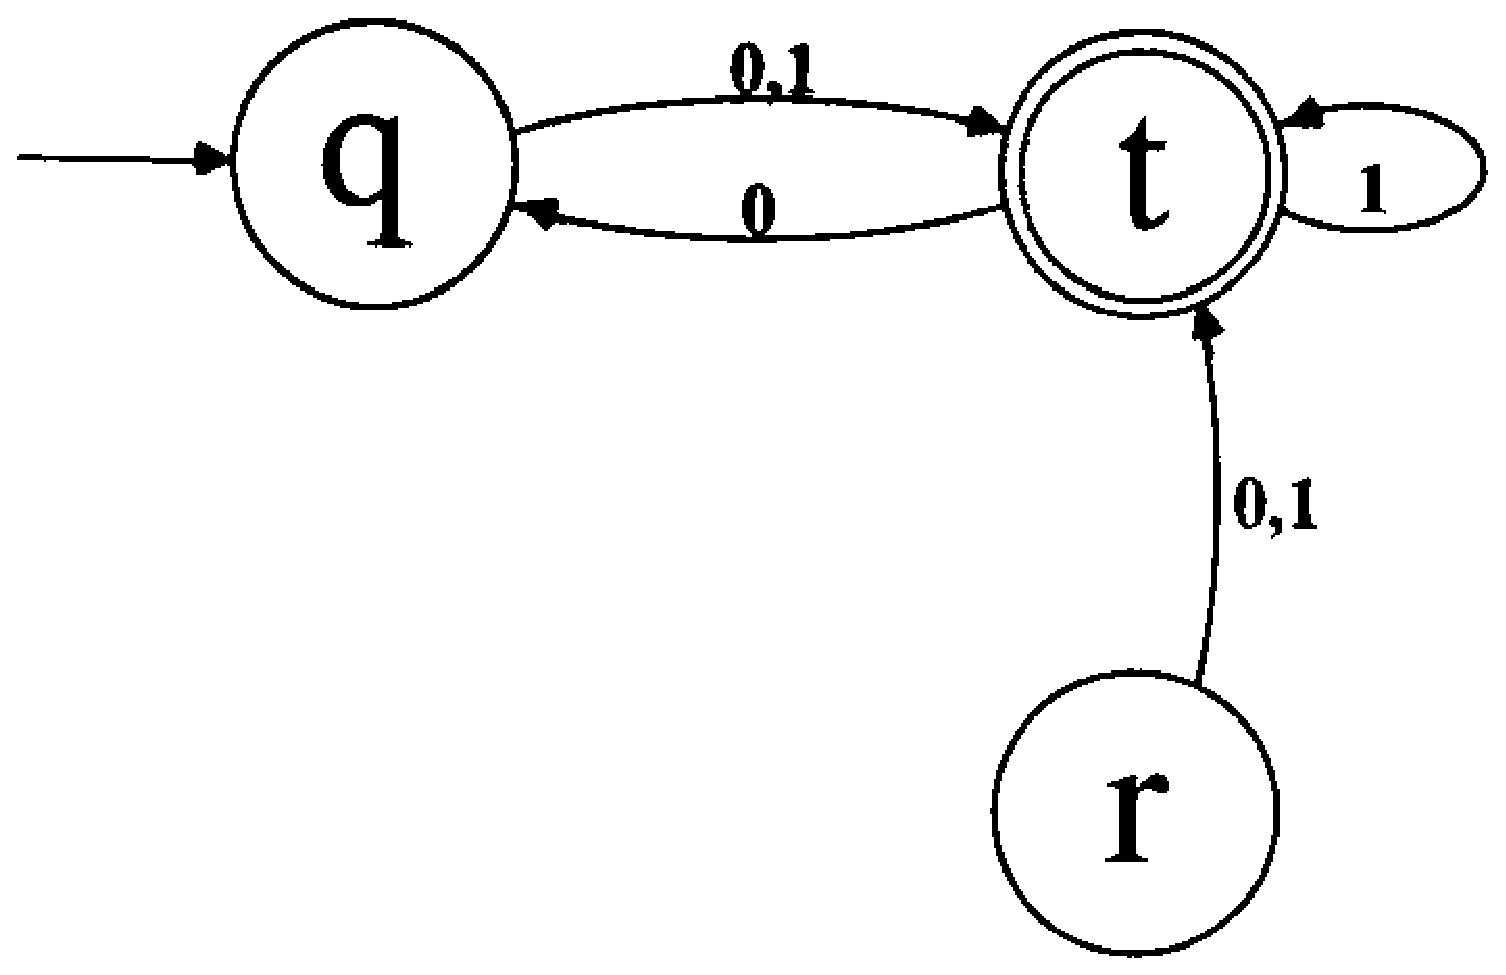
\epsfig{figure=ToFAfigures/fig3-1.eps,width=3in}}
\caption{The automaton discussed in Example 3.1}\label{fig-3.1}
\end{figure}

\subsection*{Example 3.2}

Consider the four-state DFA over $\{\pmb{a},\pmb{b}\}$ in which $s_0$ is the start and
only final state, defined in Figure \ref{fig-3.2}. This automaton is clearly connected,
but it is still not optimal. This machine accepts all strings whose length is a
multiple of 3, and $s_1$ and $s_2$ are really ``remembering'' the same
information, that is, that we currently have read a string that is one more than
a multiple of 3. The fact that some strings that end in $\pmb a$ are sent to $s_1$,
while those that end in $\pmb b$ may be sent to $s_2$, is of no real importance; we
do not have to ``remember'' what the last letter in the string actually was in
order to correctly accept the given language. The states $s_1$ and $s_2$ are in
some sense \emph{equivalent}\index{equivalent!DFA states}, since they are performing the same
function. The careful reader may have noticed that this language could have been
recognized with a three-state machine, in which a single state combines the
functions of $s_1$ and $s_2$.

Now consider the automaton shown in Figure \ref{fig-3.3}, in which there are three
superfluous states. This automaton accepts the same language as the DFA in
Figure \ref{fig-3.2}, but this time not only are $s_1$ and $s_2$ performing the same
function, but $s_3$ and $s_4$ are ``equivalent,'' and $s_0$ and $s_5$ are both
``remembering'' that there has been a multiple of three letters seen so far.
Note that it is not enough to check that $s_1$ and $s_2$ take you to exactly the
same places (as was the case in the first example); in this example, the arrows
coming out of $s_1$ and $s_2$ do \emph{not} point to the same places. The
important thing is that, when leaving $s_1$ or $s_2$, when $\pmb a$ is seen, we go to
\emph{equivalent} states, and when processing $\pmb b$ from $s_1$ or $s_2$,
we also go to \emph{equivalent} states. However, deciding whether two states are
equivalent or not is perhaps a little less straightforward than it may at first
seem. This sets the stage for the appropriate definition of equivalence.

% Figure 3.2
\begin{figure}
\centerline{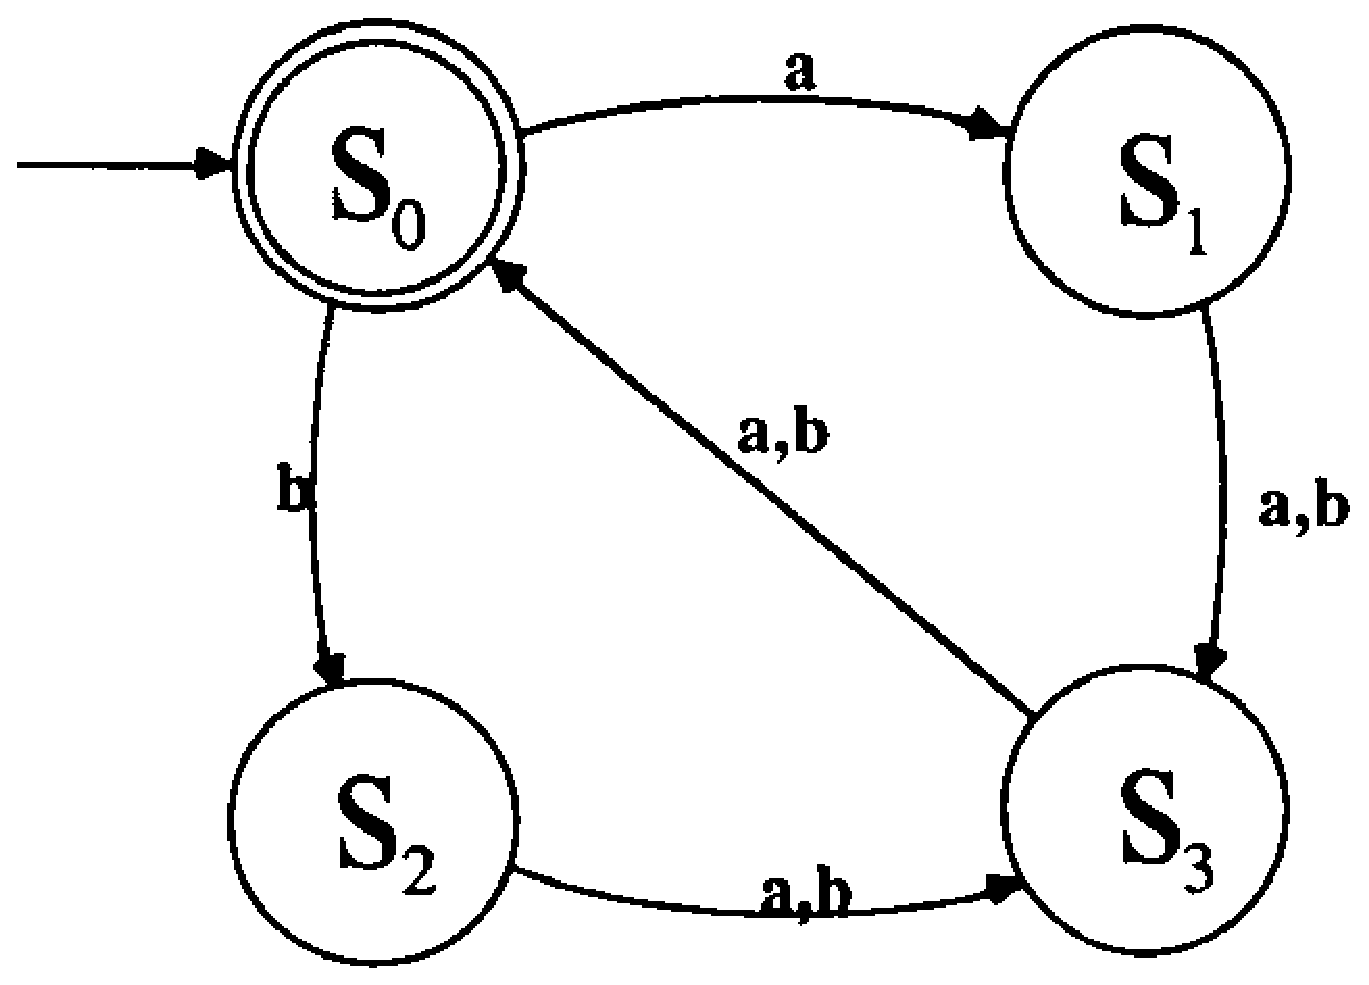
\epsfig{figure=ToFAfigures/fig3-2.eps,width=2.8in}}
\caption{The first automaton discussed in Example 3.2}\label{fig-3.2}
\end{figure}

% Figure 3.3
\begin{figure}
\centerline{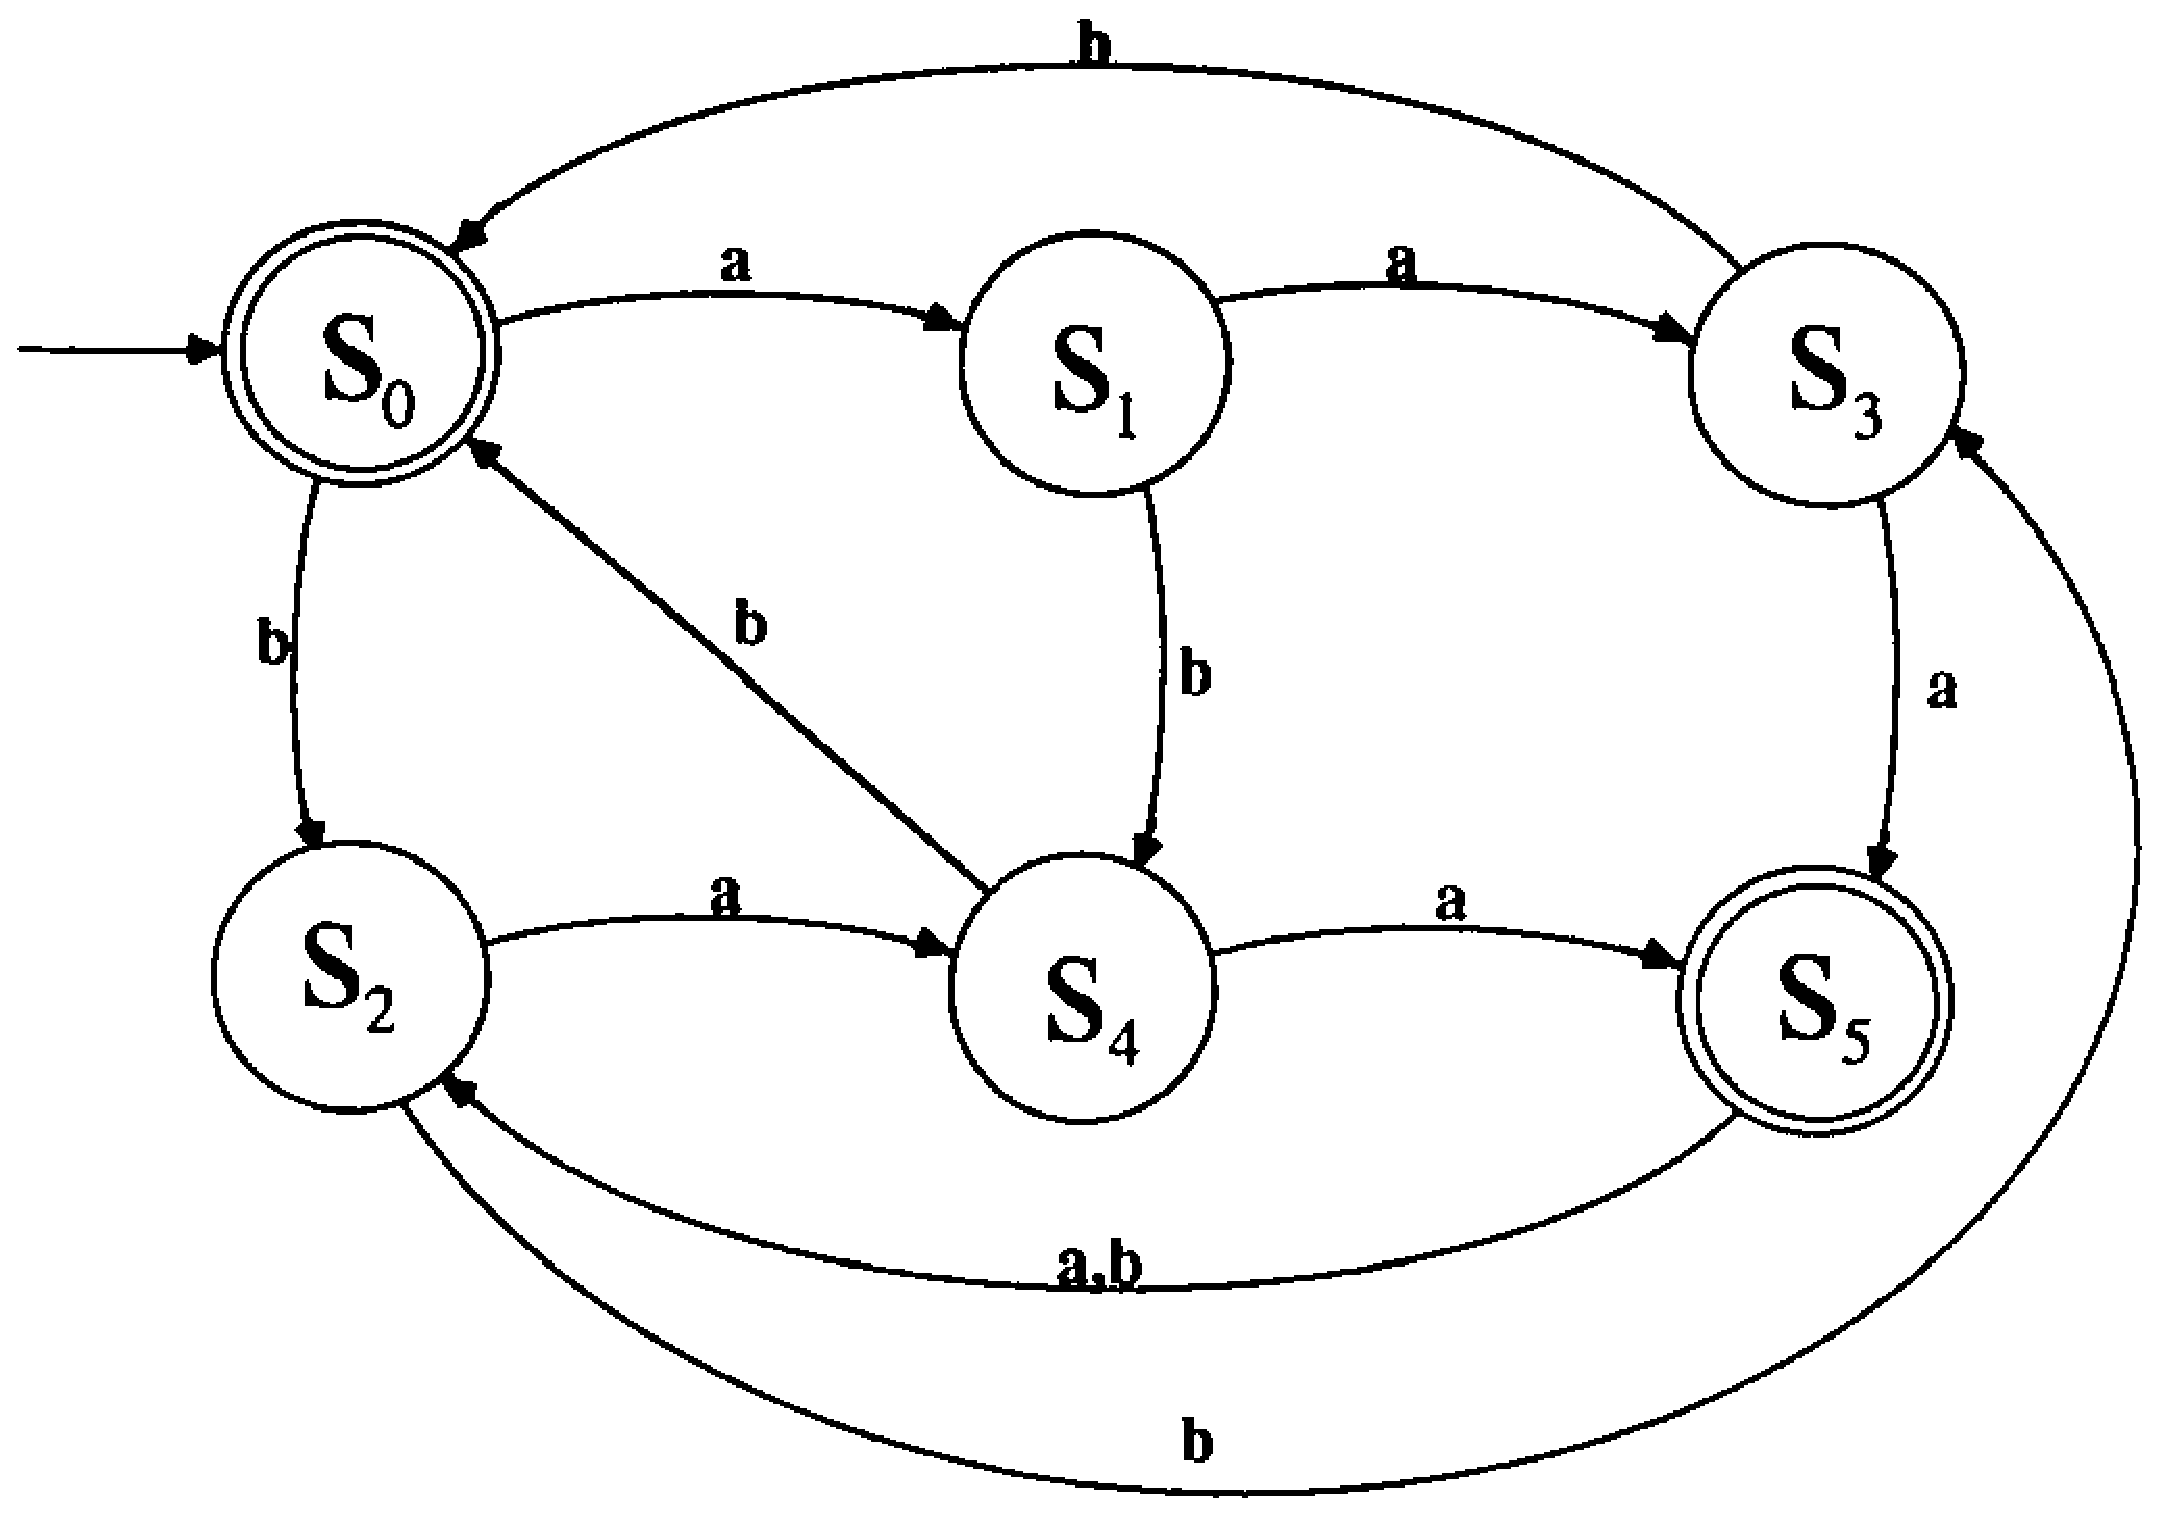
\epsfig{figure=ToFAfigures/fig3-3.eps,width=5in}}
\caption{The second automaton discussed in Example 3.2}\label{fig-3.3}
\end{figure}

% Definition 3.2
\begin{dfn}\label{dfn-3.2}\index{equivalent!DFA states}\index{state equivalence relation!for DFA}
Given a finite automaton $A=\langle\Sigma,S,s_0,\delta,F\rangle$, there is a relation
between the states of $A$ denoted by $E_A$, the \emph{\Index{state equivalence}}
relation on $A$, defined by \\
\centerline{$ (\forall s \in S)(\forall t \in S)(s E_A t \Leftrightarrow
(\forall x \in \Sigma^*)(\DBAR(s,x)\in F \Leftrightarrow \DBAR(t,x)\in F)) $}
\end{dfn}
In other words, we will relate $s$ and $t$ \emph{iff} it is not possible to
distinguish whether we are starting from state $s$ or state $t$; each string
$x \in \Sigma^*$ will \emph{either} take $x$ to a final state when starting from
$s$ and also take $x$ to a final state from $t$, \emph{or} neither $s$ nor $t$ will
take $x$ to a final state.

Another way of looking at this concept is to define new machines that ``look
like'' $A$, but have different start states. Given a finite automaton
$A =\langle\Sigma,S,s_0,\delta,F\rangle$ and two states $s,t \in S$, define a new
automaton $A^t =\langle\Sigma,S,t,\delta,F\rangle$ that has $t$ as a start state, and
another automaton $A^s =\langle\Sigma,S,s,\delta,F\rangle$ having $s$ as a start state.
Then $s E_A t \Leftrightarrow L(A^s) = L(A^t)$. (Why is this an equivalent
definition?) These sets of words will be used in later chapters and are referred
to as \emph{\Index{terminal sets}}. $T(A,t)$ will denote the set of all words
that reach final states from $t$, and thus
$T(A,t) = L(A^t) = \{x\ |\DBAR(t,x) \in F\}$.

In terms of the black box model presented in Chapter \ref{ch-1}, we see that we cannot
distinguish between $A^s$ and $A^t$ by placing matching strings on the input
tapes and observing the acceptance lights of the two machines. For any string,
both $A^s$ and $A^t$ will accept, or both will reject; without looking inside
the black boxes, there is no way to tell whether we are starting in state $s$ or
state $t$. This highlights the sense in which $s$ and $t$ are deemed equivalent:
we cannot distinguish between $s$ and $t$ by the subsequent behavior of the
automaton.

The modified automaton $A^t$, which gives rise to the terminal set $T(A,t)$, can
be contrasted with the modified automaton $A_t=\langle\Sigma,S,s_0,\delta,\{t\}\rangle$
from Chapter \ref{ch-2}, which recognized the initial set
$I(A,t) = \{x\ | \DBAR(s_0,x) = t\}$. Notice that initial sets are comprised of
strings that move from the start state to the distinguished state $t$, while
terminal sets are made up of strings that go from $t$ to a final state.

\subsection*{Example 3.3}

The automaton $N$ discussed in Example 2.6 (Figure \ref{fig-3.4}) has the following
relations comprising $E_N$:
\begin{center}
\begin{tabular}{l}
$s_0 E_N s_0$ \\
$s_1 E_N s_1,$ $s_1 E_N s_2,$ $s_1 E_N s_3$\\
$s_2 E_N s_1,$ $s_2 E_N s_2,$ $s_2 E_N s_3$\\
$s_3 E_N s_1,$ $s_3 E_N s_2,$ $s_3 E_N s_3$
\end{tabular}
\end{center}
This can be succinctly described by listing the equivalence classes:
\begin{center}
\begin{tabular}{l}
$[s_0]_{E_N} = \{s_0\}$ \\
$[s_1]_{E_N} = [s_2]_{E_N} = [s_3]_{E_N} = \{s_1, s_2, s_3\}$,
\end{tabular}
\end{center}
and we will abuse our notation slightly and blur the distinction
between the relation $E_N$ with the partition it generates by writing
$E_N = \{\{s_0\},\{s_1,s_2,s_3\}\}$.

% Figure 3.4
\begin{figure}
\centerline{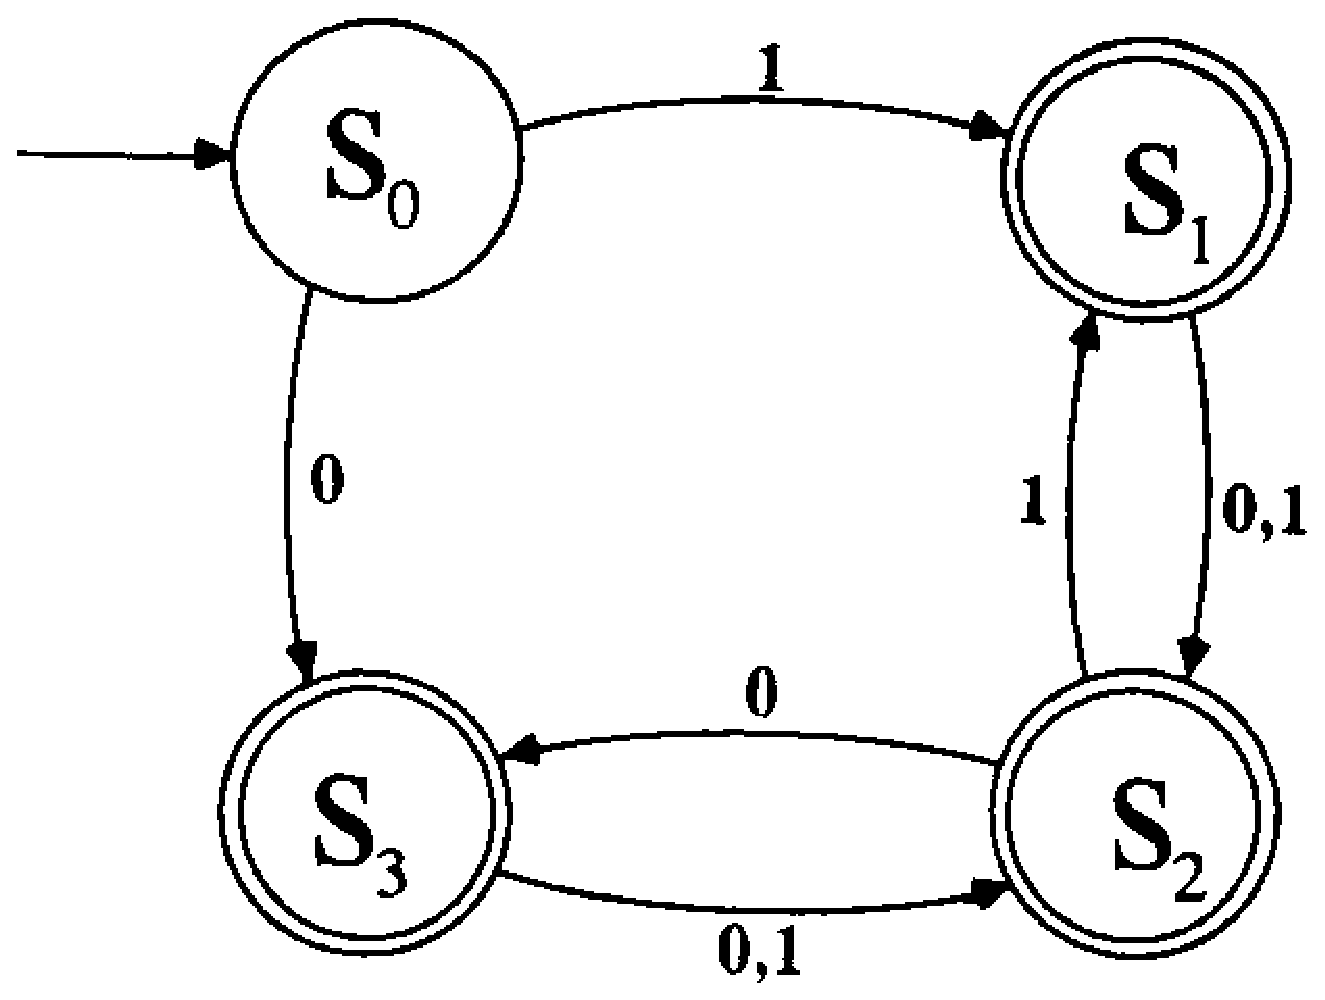
\epsfig{figure=ToFAfigures/fig3-4.eps,width=2.8in}}
\caption{The automaton N discussed in Example 3.3}\label{fig-3.4}
\end{figure}

Recall that Example 2.6 showed that the minimal machine that accepted $L(N)$
had two states; it will be seen that it is no coincidence that $E_N$ has exactly
the same number of equivalence classes.

% Definition 3.3
\begin{dfn}\label{dfn-3.3}\index{reduced!DFA}
A finite automaton $A = \langle\Sigma,S,s_0,\delta,F\rangle$ is called
\emph{reduced} iff $(\forall s,t \in S)(s E_A t \Leftrightarrow s = t)$.
\end{dfn}


In a reduced machine, $E_A$ must be the identity relation on $S$, and in this
case each equivalence class will contain only a single element.

\subsection*{Example 3.4}

The automaton $N$ in Figure \ref{fig-3.4} is not reduced, since Example 3.3 shows that
$[s_2]_{E_N}$ contains three states. On the other hand, the automaton $A$
displayed in Figure \ref{fig-3.5}a is reduced since $[s_0]_{E_A}=\{s_0\}$ and
$[s_1]_{E_A}=\{s_1\}$. The concepts of homomorphism and isomorphism will play an
integral part in justifying the correctness of the algorithms that produce the
optimal DFA for a given language. We need to formalize what we mean when we say
that two automata are ``the same.'' The following examples illustrate the
criteria that must exist between similar machines.

\subsection*{Example 3.5}

We now consider the automaton $B$ shown in Figure \ref{fig-3.5}b, which looks suspiciously
like the DFA $A$ given in Figure \ref{fig-3.5}a. In fact, it is basically the ``same''
machine. While it has been oriented differently (which has no effect on the $\delta$
function), and the start state has been labeled $q_0$ rather than $s_0$, and the
final state is called $q_1$ rather than $s_1$, $A$ and $B$ are otherwise
``identical.'' For such a \emph{\Index{relabeling}} to truly reflect the
same automaton structure, certain conditions must be met, as illustrated in the
following examples.

\subsection*{Example 3.6}

Consider machine $C$, defined by the state transition diagram given in Figure
\ref{fig-3.5}c. This machine is identical to $B$, except for the position of the start
state. However, it is not the same machine as B, since it behaves differently
(and in fact accepts a different language). Thus we see that it is important for
the start state of one machine to correspond to the start state of the other
machine. Note that we cannot circumvent this by letting $q_0$ correspond to
$s_1$, and $q_1$ correspond to $s_0$, since other problems will develop, as
shown next in Example 3.7.

% Figure 3.5
\begin{figure}
\centerline{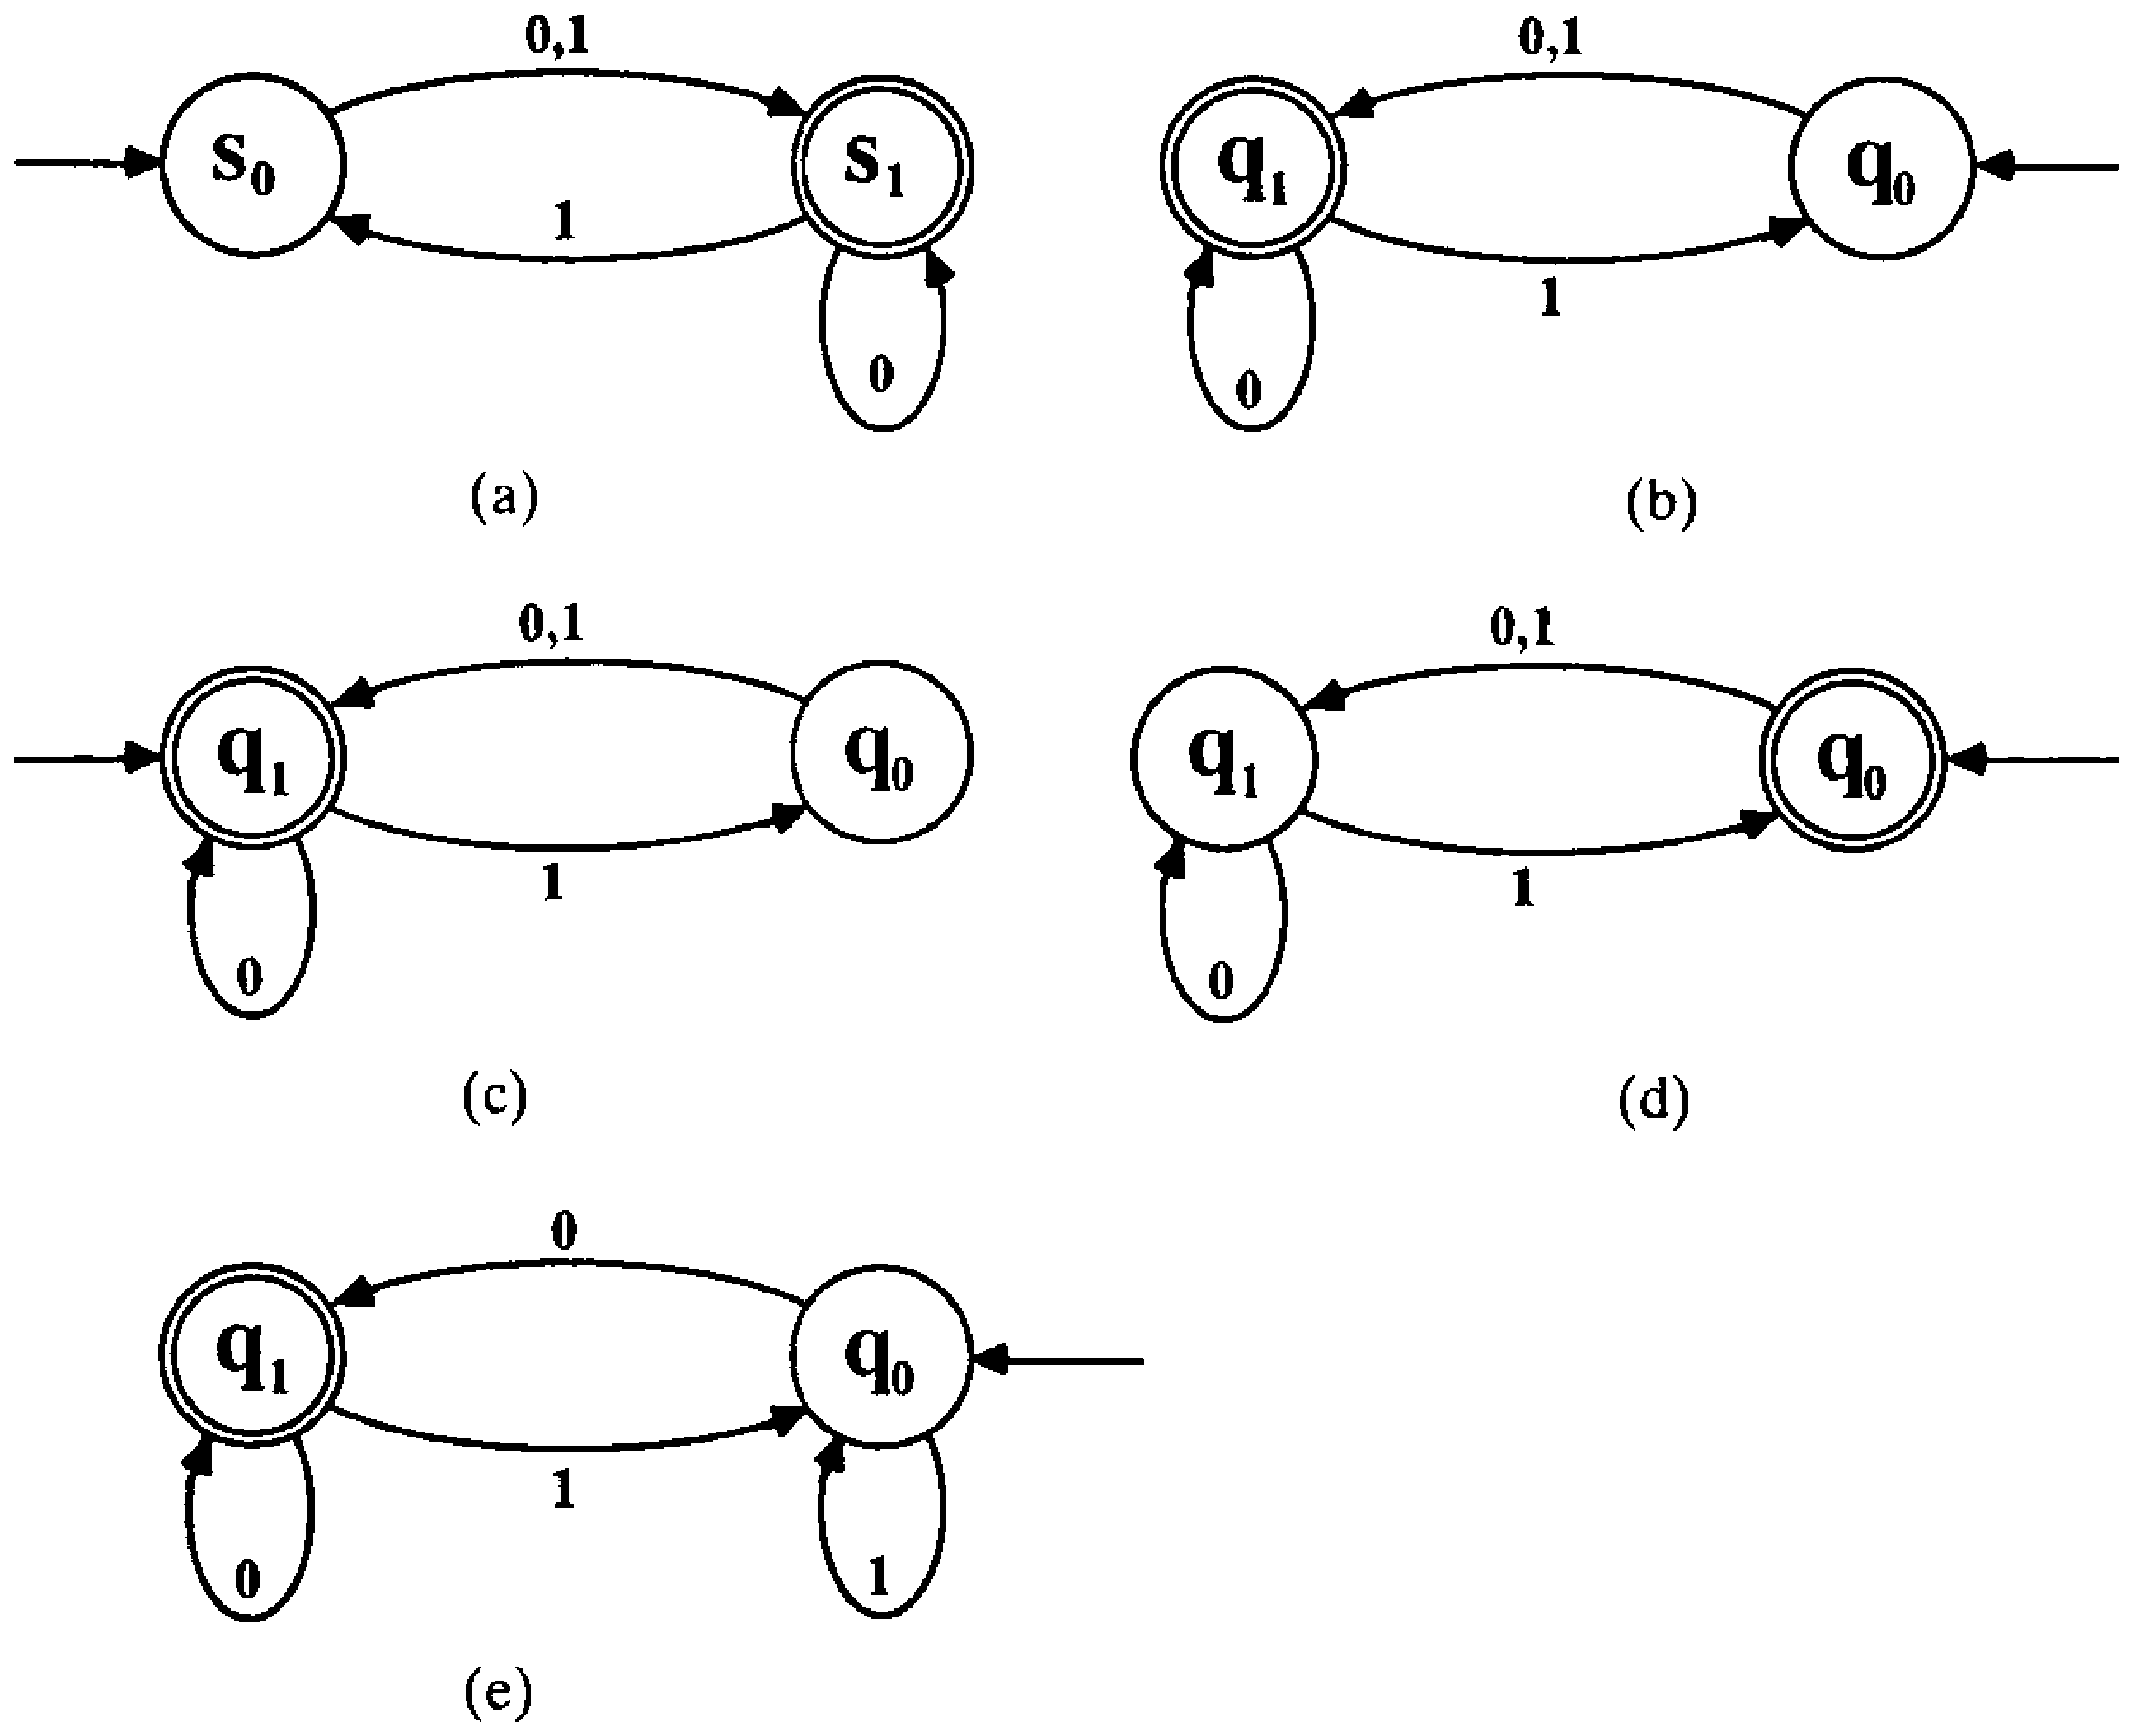
\epsfig{figure=ToFAfigures/fig3-5.eps,width=6in}}
\caption{(a) The automaton A; (b) The automaton B; (c) The automaton C; (d) The
automaton D; (e) The automaton E}\label{fig-3.5}
\end{figure}

\subsection*{Example 3.7}

Let machine $D$ be defined by the state transition diagram given in Figure \ref{fig-3.5}d.
The automata $B$ and $D$ (Figures \ref{fig-3.5}b and \ref{fig-3.5}d) look much the same, with start
states corresponding, but they are not the same (and will in fact accept
different languages), because we cannot get the final states to correspond
correctly. Even if we do get the start and final states to agree, we still have
to make sure that the transitions correspond. This is illustrated in the next
example.

\subsection*{Example 3.8}

Consider the machine $E$ given in Figure \ref{fig-3.5}e. In this automaton, when leaving
the start state, we travel to a final state if we see $\pmb{0}$, and remain at the
start state (which is nonfinal) if we see $\pmb{1}$; this is different from what
happened in machine $A$, where we traveled to a final state regardless of
whether we saw $\pmb{0}$ or $\pmb{1}$. Thus it is seen that we not only have to find
a correspondence (which can be thought of as a function $\mu$) between the
states of our two machines, but we must do this in a way that satisfies the
above three conditions (or else we cannot claim the machines are ``the same'').
This is summed up in the following definition of a \emph{homomorphism}.

% Definition 3.4
\begin{dfn}\label{dfn-3.4}\index{homomorphism!between DFAs}\index{finite automaton!homomorphism}
Given two finite automata, $A=\langle\Sigma,S_A,s_{0_A},\delta_A,F_A\rangle$ and
$B=\langle\Sigma,S_B,s_{0_B},\delta_B,F_B\rangle$, and a function
$\mu:\ S_A \rightarrow S_B$. $\mu$ is called a \emph{finite automata
homomorphism} from $A$ to $B$ iff the following three conditions hold:
\begin{enumerate}[i.]
\item $\mu(s_{0_A}) = s_{0_B}.$
\item $(\forall s \in S_A)(s \in F_A \Leftrightarrow \mu(s) \in F_B).$
\item $(\forall s \in S_A)(\forall \pmb{a} \in \Sigma)(\mu(\delta_A(s,\pmb{a}))
	= \delta_B(\mu(s),\pmb{a})).$
\end{enumerate}
\end{dfn}

Note that $\mu$ is called a homomorphism from $A$ to $B$, but it is actually a
function between state sets, that is, from $S_A$ to $S_B$.

\subsection*{Example 3.9}

Machines $A$ and $B$ in Example 3.5 are homomorphic, since the homomorphism
$\mu$$: \{s_0,s_1\}\rightarrow\{q_0,q_1\}$ defined by $\mu(s_0)=q_0$ and
$\mu(s_1)=q_1$ satisfies the three conditions.

The following example shows that even if we can find a homomorphism that
satisfies the 3 conditions the machines might not be the same.

\subsection*{Example 3.10}

% Figure 3.6
\begin{figure}
\centerline{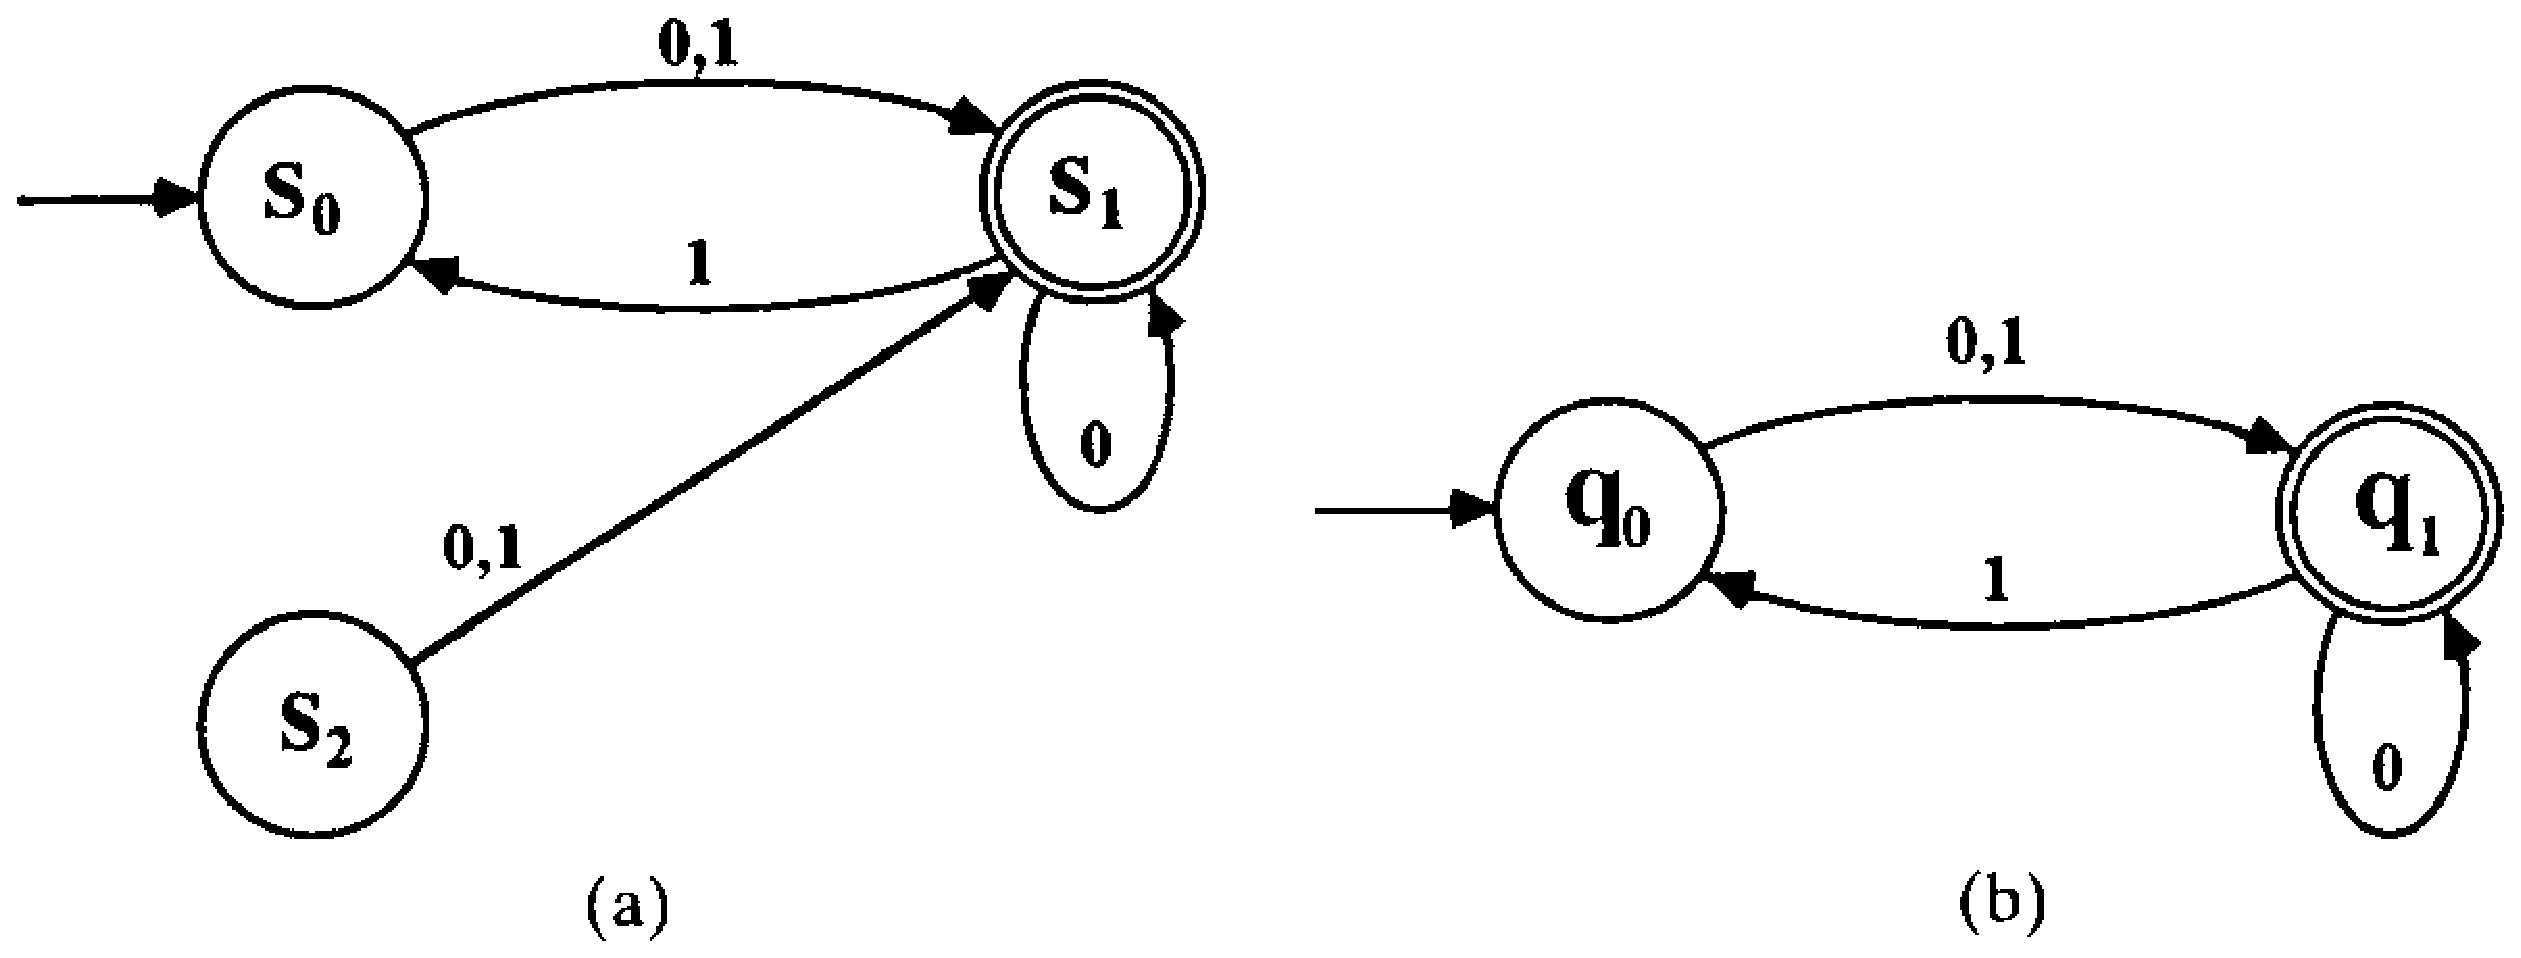
\epsfig{figure=ToFAfigures/fig3-6.eps,width=6in}}
\caption{(a) The DFA $M$ discussed in Example 3.10 (b) The DFA $N$
discussed in Example 3.10}\label{fig-3.6}
\end{figure}

Let $M =\langle\Sigma,\{s_0,s_1,s_2\},s_0,\delta_M,\{s_1\}\rangle$ and
$N =\langle\Sigma,\{q_0,q_1\},q_0,\delta_N,\{q_1\}\rangle$ be given by the state
transition diagrams in Figures \ref{fig-3.6}a and \ref{fig-3.6}b. Define a homomorphism
$\psi$$:\ \{s_0,s_1,s_2\}\rightarrow\{q_0,q_1\}$ by $\psi(s_0)=q_0$,
$\psi(s_1)=q_1$, and $\psi(s_2)=q_0$. Note that the start state maps to the
start state, final states map to final states (and nonfinal states map to
nonfinal states), and, furthermore, the transitions agree. Here is the statement
that the $\pmb{0}$ transition out of state $s_0$ is consistent:
$$ \psi(\delta_M(s_0,\pmb{0}))=\psi(s_1)=q_1=\delta_N(q_0,\pmb{0})=\delta_N(\psi(s_0),\pmb{0}) $$
Note that this really \emph{does} say that the transition labeled $\pmb{0}$
leaving the start state conforms; $s_0$ has a $\pmb{0}$-transition pointing to
$s_1$, and so the $\pmb{0}$-transition from $\psi(s_0)$ should point to $\psi(s_1)$
(that is, $q_0$ should point to $q_1$). But the transition taken from $s_0$
upon seeing a $\pmb{0}$, in our notation, is $\delta_M(s_0,0)$, and the place
$q_0$ goes to is $\delta_N(q_0,0)$. We wish to make sure that the state in $N$
corresponding to where the $\pmb{0}$-transition from $s_0$ points, denoted by
$\psi(\delta_M(s_0,0))$, agrees with the state to which $q_0$ points. Hence we
require $\psi(\delta_M(s_0,0)) = \delta_N(q_0,0)$. In the last formula, $q_0$ was
chosen because that was the state corresponding to $s_0$; that is,
$\psi(s_0)=q_0$. Hence, in our formal notation, we were really checking
$\psi(\delta_M(s_0,0)) = \delta_N(\psi(s_0),0)$. Hence, we see that rule (iii)
requires us to check all transitions leading out of all states for all letters;
that is, $(\forall s \in S_M)(\forall a \in \Sigma)(\psi(\delta_M(s,a)) =
\delta_N(\psi(s),a))$. Applying this rule to each choice of letters $\pmb{a}$ and
states $s$, we have
\begin{center}
\begin{tabular}{l}
$\psi(\delta_M(s_0,\pmb{0}))=\psi(s_1)=q_1=\delta_N(q_0,\pmb{0})=\delta_N(\psi(s_0),\pmb{0})$ \\
$\psi(\delta_M(s_0,\pmb{1}))=\psi(s_1)=q_1=\delta_N(q_0,\pmb{1})=\delta_N(\psi(s_0),\pmb{1})$ \\
$\psi(\delta_M(s_1,\pmb{0}))=\psi(s_1)=q_1=\delta_N(q_1,\pmb{0})=\delta_N(\psi(s_1),\pmb{0})$ \\
$\psi(\delta_M(s_1,\pmb{1}))=\psi(s_0)=q_0=\delta_N(q_1,\pmb{1})=\delta_N(\psi(s_1),\pmb{1})$ \\
$\psi(\delta_M(s_2,\pmb{0}))=\psi(s_1)=q_1=\delta_N(q_0,\pmb{0})=\delta_N(\psi(s_2),\pmb{0})$ \\
$\psi(\delta_M(s_2,\pmb{1}))=\psi(s_1)=q_1=\delta_N(q_0,\pmb{1})=\delta_N(\psi(s_2),\pmb{1})$
\end{tabular}
\end{center}
Hence $\psi$ is a homomorphism between $M$ and $N$ even though $M$ has three
states and $N$ has two states. While the existence of a homomorphism is not
enough to ensure that the machines are ``the same,'' the exercises for this
chapter indicate that the existence of a homomorphism \emph{is} enough to ensure that
the machines are equivalent. The extra condition we need to guarantee that the
machines are identical\index{identical DFAs} (except for a trivial renaming of the states) is that
$\psi$ be a \emph{\Index{bijection}}.

% Definition 3.5
\begin{dfn}\label{dfn-3.5}\index{isomorphism!between DFAs}\index{finite automaton!isomorphism}
Given two finite automata $A=\langle\Sigma,S_A,s_{0_A},\delta_A,F_A\rangle$ and
$B=\langle\Sigma,S_B,s_{0_B},\delta_B,F_B\rangle$, and a function
$\mu:\ S_A \rightarrow S_B$, $\mu$ is called a \emph{finite automata
isomorphism} from $A$ to $B$ iff the following five conditions hold:
\begin{enumerate}[i.]
\item $\mu(s_{0_A}) = s_{0_B}$.
\item $(\forall s \in S_A)(s \in F_A \Leftrightarrow \mu(s) \in F_B)$.
\item $(\forall s \in S_A)(\forall \pmb{a} \in \Sigma)(\mu(\delta_A(s,\pmb{a}))
	= \delta_B(\mu(s),\pmb{a}))$.
\item $\mu$ is a one-to-one function from $S_A$ to $S_B$.
\item $\mu$ is onto $S_B$.
\end{enumerate}
\end{dfn}

\subsection*{Example 3.11}

$\mu$ from Example 3.9 is an isomorphism. Example 3.5 illustrated that the
automaton $A$ was essentially ``the same'' as $B$ except for the way the states
were named. Note that $\mu$ can be thought of as the recipe for relabeling the
states of $A$ to form a machine that would then be in the very strictest sense
absolutely \emph{identical} to $B$. $\psi$ from Example 3.10 is not an
isomorphism because it is not one to one.

% Definition 3.6
\begin{dfn}\label{dfn-3.6}
Given two finite automata $A=\langle\Sigma,S_A,s_{0_A},\delta_A,F_A\rangle$ and
$B=\langle\Sigma,S_B,s_{0_B},\delta_B,F_B\rangle$, $A$ is said to be
\emph{\Index{isomorphic}} to $B$ iff there exists a finite automata isomorphism
between $A$ and $B$, and we will write $A \cong B$.
\end{dfn}

\subsection*{Example 3.12}

Machines $A$ and $B$ from Examples 3.4 and 3.5 are isomorphic. Machines $M$ and
$N$ from Example 3.10 are not isomorphic (and not just because the particular
function $\psi$ fails to satisfy the conditions; we must actually prove that \emph{no}
function exists that qualifies as an isomorphism between $M$ and $N$).

Now that we have rigorously defined the concept of two machines being
``essentially identical,'' we can prove that, given a language $L$, any reduced
and connected machine $A$ accepting $L$ must be \emph{minimal}, that is, have as few
states as possible for that particular language. We will prove this assertion by
showing that any such $A$ is isomorphic to $A_{R_L}$, which was shown in
Corollary \ref{cor-3.2} to be the ``smallest'' possible machine for $L$.


% Theorem 3.1
\begin{thm}\label{thm-3.1}
Let $L$ be any FAD language over an alphabet $\Sigma$, and let
$A=\langle\Sigma,S,s_0,\delta,F\rangle$ be any reduced and connected automaton
that accepts $L$. Then $A \cong A_{R_L}$.

\emph{Proof.} We must try to define a reasonable function $\mu$ from the states
of $A$ to the states of $A_{R_L}$ (which you should recall corresponded to
equivalence classes of $R_L$). A natural way to define $\mu$ (which happens to
work!) is: For each $s \in S$, find a string $x_s \in \Sigma^* \ni
\DBAR(s_0,x_s) = s$. (Since A is connected, we are guaranteed to find such an
$x_s$. In fact, there may be many strings that take us from $s_0$ to $s$; choose
any one of them, and call it $x_s$.) We need to map $s$ to some equivalence
class of $R_L$; the logical choice is the class containing $x_s$. Thus we define
$$ \mu(s)=[x_s]_{R_L} $$
An immediate question comes to mind: There may be several strings that we could
use for $x_s$; does it matter which one we choose to find the equivalence class?
It would not do if, say, $R_L$ consisted of two equivalence classes, the
even-length strings = $[\pmb{11}]_RL$ and the odd-length strings =
$[\pmb{0}]_{R_L}$, and both $\DBAR(s_0,\pmb{0})$ and $\DBAR(s_0,\pmb{11})$ equaled $s$. Then, on
the one hand, $\mu(s)$ should be $[\pmb{0}]_{R_L}$ and, on the other hand, it should
be $[\pmb{11}]_{R_L}$. $\mu$ must be a function; it cannot send $s$ to two different
equivalence classes. Note that there would be no problem if $\DBAR(s_0,\pmb{11})=s$ 
and $\DBAR(s_0,\pmb{1111}) = s$, since $[\pmb{11}]_{R_L}=[\pmb{1111}]_{R_L}$, both of which
represent the set of all even-length strings. Here $x_s$ could be $\pmb{11}$, or
it could be $\pmb{1111}$, and there is no inconsistency in the way in which
$\mu(s)$ is defined; in either case, $s$ is mapped by $\mu$ to the class of
even-length strings. Thus we must first show:
\begin{enumerate}
\item $\mu$ is well-defined (which means it is defined everywhere, and the
definitions are consistent; that is, if there are two choices for $x_s$, say,
$y$ and $z$, then $[y]_{R_L}=[z]_{R_L}$). Since $A$ is connected, each state $s$
can be reached by some string $x_s$; that is,
$(\forall s \in S)(\exists x_s \in \Sigma^*)(\DBAR(s_0,x_s) = s)$, and so there
is indeed (at least) one equivalence class (namely $[x_s]_{R_L}$) to which $s$ maps
under $\mu$. We therefore have $\mu(s)=[x_s]_{R_L}$. Thus $\mu$ is defined
everywhere. We must still make sure that $\mu$ is not multiply defined: Let
$x,y \in \Sigma^*$ and assume $\DBAR(s_0,x)=\DBAR(s_0,y)$. Then
\begin{center}
\begin{tabular}{rcl}
$\DBAR(s_0,x)=\DBAR(s_0,y)$ & $\Rightarrow$ & (by definition of =) \\
$(\forall u \in \Sigma^*)(\DBAR(\DBAR(s_0,x),u) \in F \Leftrightarrow 
\DBAR(\DBAR(s_0,y),u) \in F)$ & $\Rightarrow$ & (by Theorem \ref{thm-1.1}) \\
$(\forall u \in \Sigma^*)(\DBAR(s_0,xu) \in F \Leftrightarrow
\DBAR(s_0,yu) \in F)$ & $\Rightarrow$ & (by definition of $L$) \\
$(\forall u \in \Sigma^*)(xu \in L \Leftrightarrow yu \in L)$ & $\Rightarrow$ &
(by definition of RL) \\
$x\ R_L y$ & $\Rightarrow$ & (by definition of [ ]) \\
$[x]_{R_L} = [y]_{R_L}$ &&
\end{tabular}
\end{center}

Thus, if both $x$ and $y$ take us from $s_0$ to $s$, then it does not matter
whether we let $\mu(s)$ equal $[x]_{R_L}$ or $[y]_{R_L}$, since they are
identical. $\mu$ is therefore a bona fide function.

\item $\mu$ is onto $S_{R_L}$. Every equivalence class must be the image of some
state in $S$, since $(\forall [x]_{R_L}\in S_{R_L})([x]_{R_L}=\mu(\DBAR(s_0,x)))$,
and so $\DBAR(s_0,x)$ maps to $[x]_{R_L}$.

\item $\mu(s_0) = s_{0_{R_L}}$
$$ s_{0_{R_L}} = [\lambda]_{R_L} = \mu(\DBAR(s_0,\lambda)) = \mu(s_0) $$

\item Final states map to final states; that is,
$(\forall s \in S)(\mu(s) \in F_{R_L} \Leftrightarrow s \in F)$. Choose an
$s \in S$ and pick a corresponding $x_s \in \Sigma^*$ such that
$\DBAR(s_0,x_s) = s$. Then
\begin{center}
\begin{tabular}{rcl}
$s \in F$ & $\Leftrightarrow$ & (by definition of $x_s$, and Definition \ref{dfn-1.14}) \\
$x_s \in L(A)$ & $\Leftrightarrow$ & (by definition of L) \\
$x_s \in L$ & $\Leftrightarrow$ & (by definition of $F_{R_L}$) \\
$[x_s]_{R_L} \in F_{R_L}$ & $\Leftrightarrow$ & (by definition of $\mu$) \\
$\mu(s) \in F_{R_L}$ &&
\end{tabular}
\end{center}

\item The transitions match up; that is,
$(\forall s \in S)(\forall a \in \Sigma)(\mu(\delta(s,a)) =
\delta_{R_L}(\mu(s),a))$. Choose an $s \in S$ and pick a corresponding
$x_s \in \Sigma^*$ such that $\DBAR(s_0,x_s) = s$. Note that this implies that
$[x_s]=\mu(s)=\mu(\DBAR(s_0,x_s))$. Then
\begin{center}
\begin{tabular}{rcl}
$\mu(\delta(s,a))$ & $=$ & (by definition of $x_s$) \\
$\mu(\delta(\DBAR(s_0,x_s),a))$ & $=$ & (by Theorem \ref{thm-1.1}) \\
$\mu(\DBAR(s_0,x_s a))$ & $=$ & (by definition of $\mu$) \\
$[x_s a]_{R_L}$ & $=$ & (by definition of $\delta_{R_L}$) \\
$\delta_{R_L}([x_s]_{R_L},a)$ & $=$ & (by definition of $\mu$ and $x_s$) \\
$\delta_{R_L}(\mu(s),a)$ &&
\end{tabular}
\end{center}
So far we have not needed the fact that $A$ was reduced. In fact, we have now
proved that $\mu$ is a homomorphism from $A$ to $A_{R_L}$ as long as $A$ is
merely connected. However, if $A$ is reduced, we can show:

\item $\mu$ is one to one; that is, if $\mu(s)=\mu(t)$, then $s=t$. Let
$s,t \in S$ and assume $\mu(s)=\mu(t)$.
\begin{center}
\begin{tabular}{rcl}
$\mu(s) = \mu(t)$ & $\Rightarrow$ & (by definition of $=$) \\
$(\forall u \in \Sigma^*)(\DBAR_{R_L}(\mu(s),u)=\DBAR_{R_L}(\mu(t),u))$ &
$\Leftrightarrow$ & [by property (5), induction] \\
$(\forall u \in \Sigma^*)(\mu(\DBAR(s,u))=\mu(\DBAR(t,u)))$ & $\Rightarrow$ &
(by definition of $=$) \\
$(\forall u \in \Sigma^*)(\mu(\DBAR(s,u))\in F_{R_L} \Leftrightarrow
\mu(\DBAR(t,u))\in F_{R_L})$ & $\Leftrightarrow$ & [by property (4) above] \\
$(\forall u \in \Sigma^*)(\DBAR(s,u) \in F \Leftrightarrow \DBAR(t,u) \in F)$ &
$\Leftrightarrow$ & (by definition of $E_A$) \\
$s E_A t$ & $\Leftrightarrow$ & (since $A$ is reduced) \\
$s = t$ &&
\end{tabular}
\end{center}
Thus, by results (1) through (6), $\mu$ is a well-defined homomorphism that is
also a bijection; so $\mu$ is an isomorphism and therefore $A \cong A_{R_L}$.
\end{enumerate}
\end{thm}

% Corollary 3.3
\begin{cor}\label{cor-3.3}
Let $A$ and $B$ be reduced and connected finite automata. Under these conditions,
$A$ is equivalent to $B$ iff $A \cong B$.

\emph{Proof}. If $A \cong B$, it is easy to show that $A$ is equivalent to $B$
(as indicated in the exercises, this implication is true even if $A$ and $B$ are
not reduced and connected). Now assume the hypothesis that $A$ and $B$ are
reduced and connected does hold, and that $A$ is equivalent to $B$. Since A is
minimal, $A \cong A_{R_{L(A)}}$. Similarly, $B \cong A_{R_{L(B)}}$. Since
$L(A) = L(B)$, $A_{R_{L(A)}} = A_{R_{L(B)}}$. Therefore,
$A \cong A_{R_{L(A)}} = A_{R_{L(B)}} \cong B$.
\end{cor}

\section{Minimization Algorithms}\label{sec-3.2}

From the results in the previous section, it follows that a reduced and
connected finite automaton must be minimal. This section demonstrates how to
transform an existing DFA into an equivalent machine that is both reduced and
connected and hence is the most efficient machine possible for the given
language. The designer of an automaton can therefore focus solely on producing a
machine that recognizes the correct set of strings (without regard for
efficiency), knowing that the techniques presented in this section can later be
employed to shrink the DFA to its optimal size. The concepts explored in
Chapters \ref{ch-4}, \ref{ch-5}, and \ref{ch-6} will provide further tools to
aid in the design process and corresponding techniques to achieve optimality.

% Corollary 3.4
\begin{cor}\label{cor-3.4}\index{finite automaton!minimal deterministic}
A reduced and connected deterministic finite automaton
$A =\langle\Sigma,S,s_0,\delta,F\rangle$ is minimal.

\emph{Proof.} By Theorem \ref{thm-3.1}, there is an isomorphism between $A$ and $A_{R_L}$.
Since an isomorphism is a bijection between the state sets,
$\|S\| = \|S_{R_L}\|$. By Corollary \ref{cor-3.2}, $A_{R_L}$ has the smallest number of
states, and therefore so does $A$.
\end{cor}

Thus, if we had a machine for $L$ that we could verify was reduced and
connected, we would be able to state that we had found the minimal machine
accepting $L$. We therefore would like some algorithms for determining if a
machine $M$ has these properties. We would also like to find a method for
transforming a nonoptimal machine into one with the desired properties. The
simplest transformation is from a disconnected machine to a connected machine:
given any machine $A$, we will define a connected machine $A^c$ that accepts the
same language that $A$ did; that is, $L(A) =L(A^c)$

% Definition 3.7
\begin{dfn}\label{dfn-3.7}\index{A@$A^c$ (A connected)!for DFA}
Given a finite automaton $A =\langle\Sigma,S,s_0,\delta,F\rangle$, define a new
automaton $A^c =\langle\Sigma,S^c,s^c_0,\delta^c,F^c\rangle$, called A
\emph{connected}, by
\begin{center}
\begin{tabular}{l}
$S^c =\{s\in S$ $|$ $\exists x \in \Sigma^* \ni \DBAR(s_0,x)=s\}$ \\
$s^c_0 = s_0$ \\
$F^c = F \cap S^c =\{f \in F$ $|$ $\exists x \in \Sigma^* \ni \DBAR(s_0,x) = f\}$
\end{tabular}
\end{center}
and $\delta^c$ is derived from the restriction of $\delta$ to $S^c\times\Sigma$:
$$(\forall \pmb{a} \in \Sigma)(\forall s \in S^c)(\delta^c(s, \pmb{a}) = \delta(s,\pmb{a})) $$
\end{dfn}

$A^c$ is thus simply the machine $A$ with the unreachable states ``thrown
away''; $s_0$ can be reached by $x = \lambda$, so it is a valid choice for the
start state in $A^c$. $F^c$ is simply the final states that can be reached from
$s_0$, and $\delta^c$ is the collection of transitions that still come from (and
consequently point to) states in the connected portion. Actually, $\delta^c$ was
defined to be the transitions that merely come from states in $S^c$, with no
mention of any restrictions on the range of $\delta^c$. We must have, however,
$\delta^c: S^c \times \Sigma \rightarrow S^c$; in order for $A^c$ to be well
defined, $\delta^c$ must be shown to map into the proper range. It would not do to
have a transition leading from a state in $A^c$ to a state that is not in the
new state set of $A^c$. The fact that $\delta^c$ does indeed have the desired
properties is relegated to the exercises.

\subsection*{Example 3.13}

Let $M =\langle\{\pmb{a},\pmb{b}\},\{q_0,q_1,q_2,q_3\},q_0,\delta,\{q_1,q_3\}\rangle$, as
illustrated in Figure \ref{fig-3.7}a. By inspection, the only states that can be reached
from the start state are $q_0$ and $q_3$. Hence
$M^c =\langle\{\pmb{a},\pmb{b}\},\{q_0,q_3\},q_0,\delta^c,\{q_3\}\rangle$. The resulting
automaton is shown in Figure \ref{fig-3.7}b. An algorithm for effectively computing $S^c$
will be presented later.

% Figure 3.7
\begin{figure}
\centerline{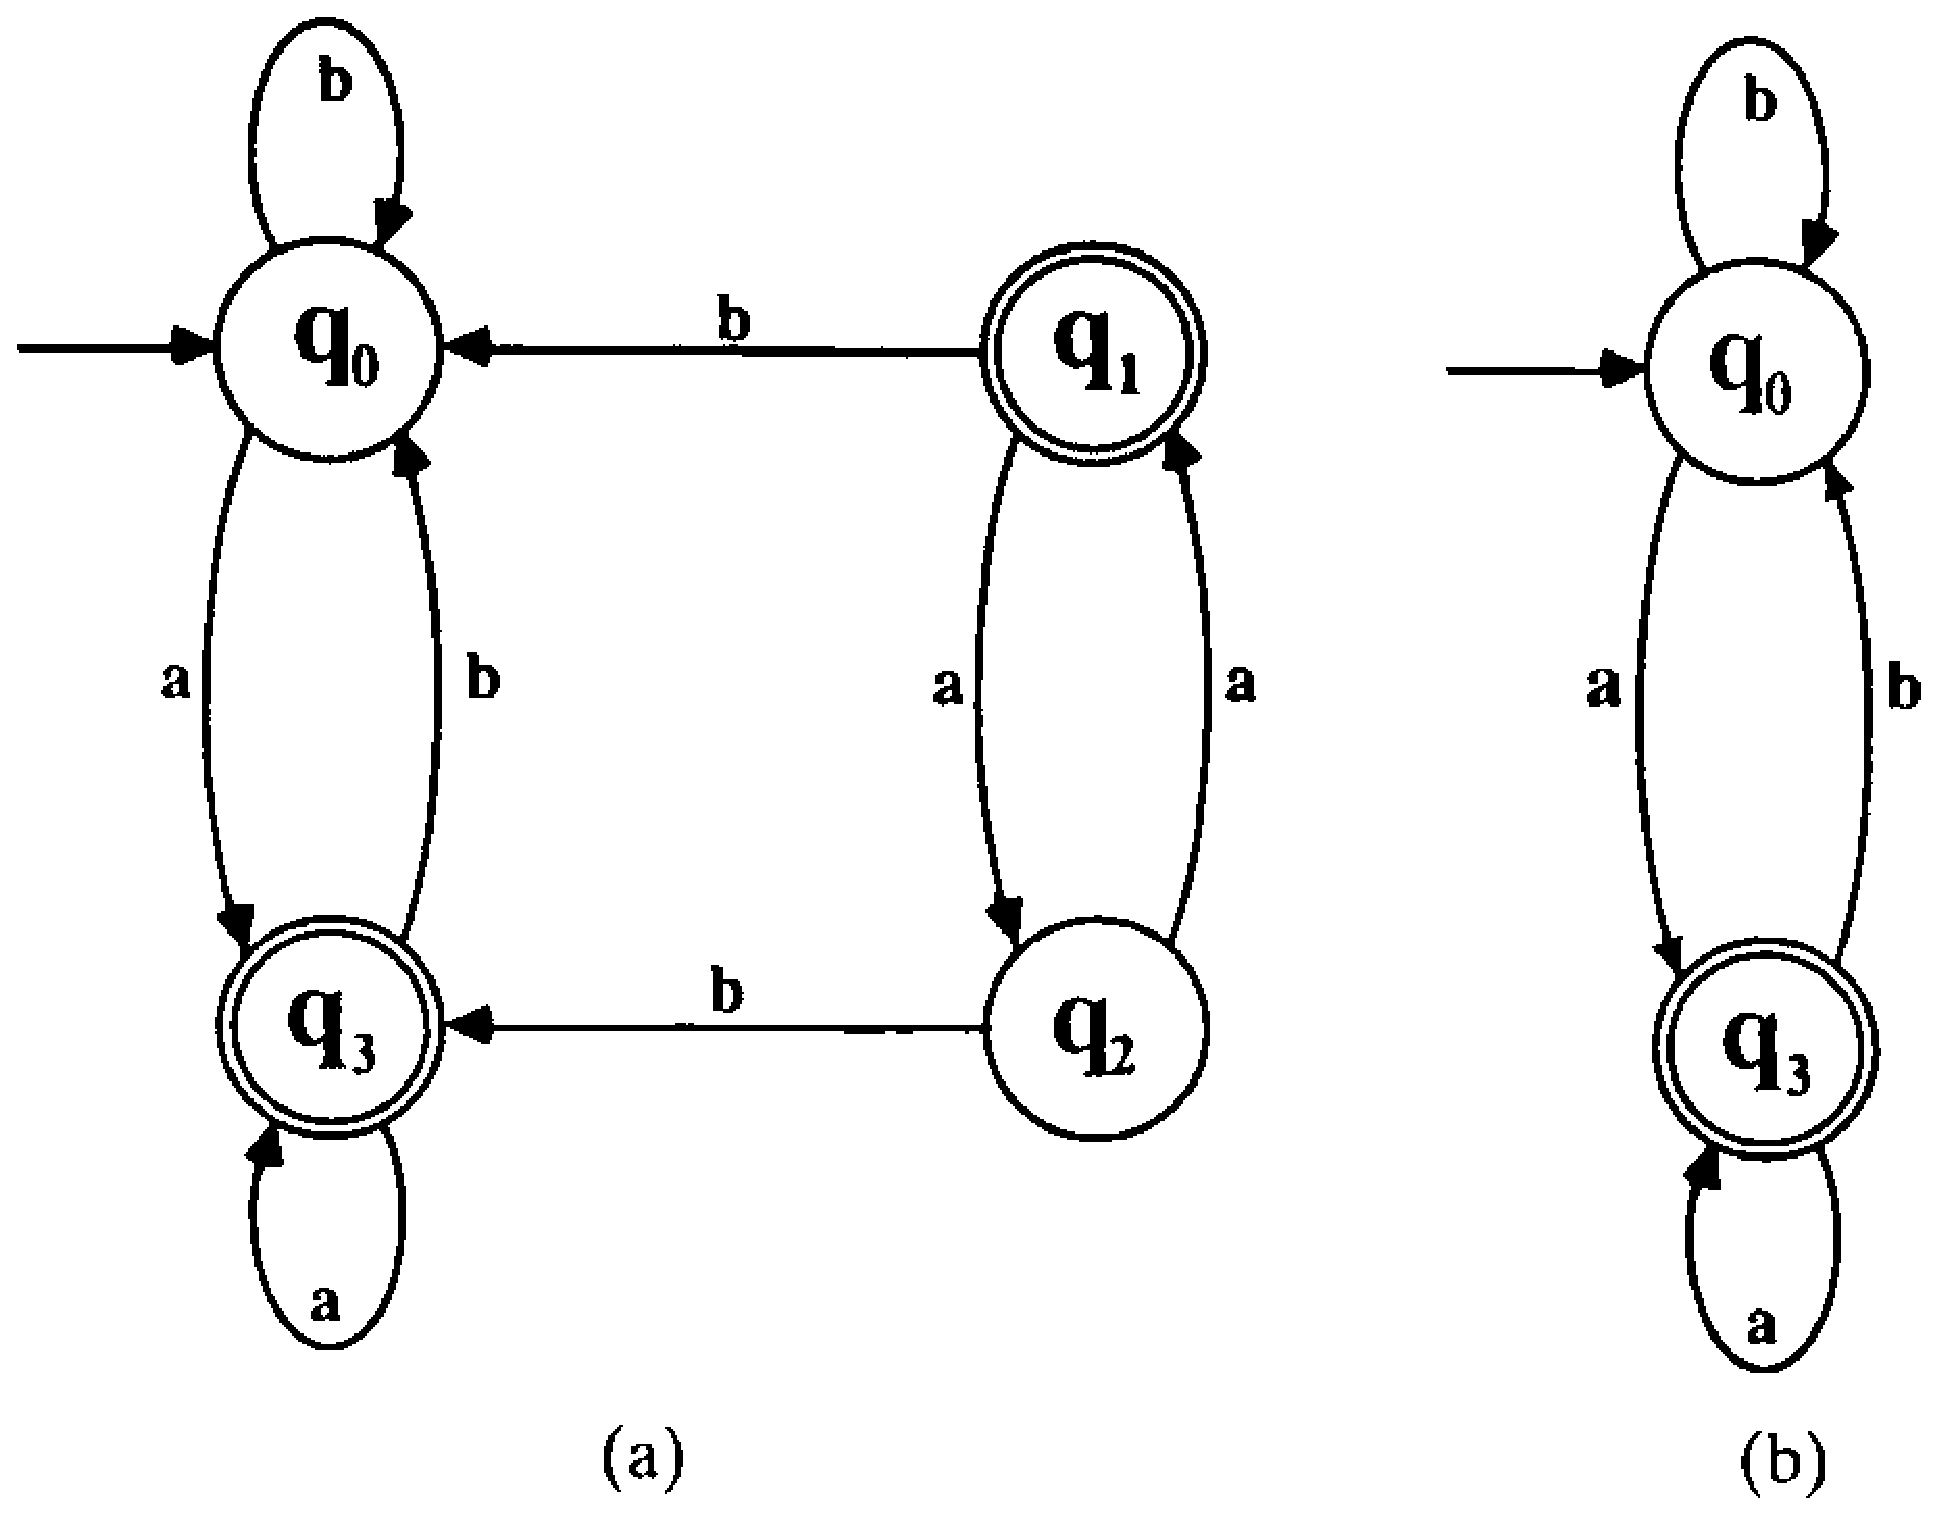
\epsfig{figure=ToFAfigures/fig3-7.eps,width=4in}}
\caption{(a) The DFA $M$ discussed in Example 3.13; (b) The DFA $M^c$ discussed
in Example 3.13}\label{fig-3.7}
\end{figure}

% Theorem 3.2
\begin{thm}\label{thm-3.2}
Given any finite automaton $A$, the new machine $A^c$ is indeed connected.

\emph{Proof.} This is an immediate consequence of the way $S^c$ was defined.
\end{thm}

Definition \ref{dfn-3.7} and Theorem \ref{thm-3.2} would be of little consequence if it were not
for the fact that $A$ and $A^c$ accept the same language. $A^c$ is in fact
equivalent to $A$, as proved in Theorem \ref{thm-3.3}.

% Theorem 3.3
\begin{thm}\label{thm-3.3}\index{equivalent!DFAs}
Given any finite automaton $A =\langle\Sigma,S,s_0,\delta,F\rangle$, $A$ and
$A^c$ are equivalent, that is, $L(A^c) = L(A)$.

\emph{Proof.} Let $x \in \Sigma^*$. Then:
\begin{center}
\begin{tabular}{rcl}
$x \in L(A)$ & $\Leftrightarrow$ & (by definition of $L$) \\
$\exists s \in S \ni (\DBAR(s_0,x) = s \wedge s \in F)$ & $\Leftrightarrow$ &
	(by definition of $S^c$) \\
$s \in S^c \wedge s \in F$ & $\Leftrightarrow$ & (by definition of $\cap$) \\
$s \in (S^c \cap F)$ & $\Leftrightarrow$ & (by definition of $F^c$) \\
$s \in F^c$ & $\Leftrightarrow$ & (by definition of $s$ [above, on line 2]) \\
$\DBAR(s_0,x) \in F^c$ & $\Leftrightarrow$ & (by definition of $\delta^c$ and
	induction) \\
$\DBAR^c(s_0,x) \in F^c$ & $\Leftrightarrow$ & (by definition of $s_0^c$) \\
$\DBAR^c(s_0^c,x) \in F^c$ & $\Leftrightarrow$ & (by definition of $L$) \\
$x \in L(A^c)$ &&
\end{tabular}
\end{center}
\end{thm}

Thus, given any machine $A$, we can find an \emph{equivalent} machine
(that is, a machine that accepts the same language as $A$) that is connected.
Furthermore, there is an algorithm that can be applied to find $A^c$ (that is,
we don't just know that such a machine exists, we actually have a method for
calculating what it is). The definition of $S^c$ implies that there is a
\emph{procedure} for finding $S^c$: one can begin enumerating the strings $x$ in
$\Sigma^*$, and by applying the transition function to each $x$, the new states
that are reached can be included in $S^c$. This is not a very satisfactory
process because there are an infinite number of strings in $\Sigma^*$ to check.
However, the indicated proof for Theorem \ref{thm-2.7} shows that, if a state can be
reached by a ``long'' string, then it can be reached by a ``short'' string.
Thus, we will only need to check the ``short'' strings. In particular,
$$ S^c \equiv \bigcup\limits_{x \in \Sigma^*} \DBAR(s_0,x) =
	\bigcup\limits_{x \in Q} \DBAR(s_0,x) $$
where $Q$ consists of the ``short'' strings:
$Q =\{x \in \Sigma^*|\ |x| < \|S\|\}$. Thus, $Q$ is the set of all strings of
length less than the number of states in the DFA. $Q$ is a finite set, and
therefore we can check all strings $x$ in $Q$ in a finite amount of time; we
therefore have an \emph{algorithm} (that is, a procedure that is guaranteed to halt)
for finding $S^c$, and consequently an algorithm for constructing $A^c$. Thus,
given any machine, we can find an equivalent machine that is connected. The
above method is not very efficient because many calculations are constantly
repeated. A better algorithm based on Definition \ref{dfn-3.10} will be presented later.

We now turn our attention to building a reduced machine from an arbitrary
machine. The following definition gives a consistent way to combine the
redundant states identified by the state equivalence relation $E_A$.

% Definition 3.8
\begin{dfn}\label{dfn-3.8}\index{A @$ A/_{E_A}$ (A modulo $E_A$)!for DFA}
Given a finite automaton $A =\langle\Sigma,S,s_0,\delta,F\rangle$, define a new
finite automaton $A/\!\!_{E_A}$, called \emph{$A$ modulo its state equivalence
relation}, by
$$ A/_{E_A} =\langle\Sigma,S_{E_A},s_{0_{E_A}},\delta_{E_A},F_{E_A}\rangle $$
where
\begin{center}
\begin{tabular}{rcl}
$S_{E_A}$ & $=$ & $\{[s]_{E_A}$ $|$ $s \in S\}$ \\
$s_{0_{E_A}}$ & $=$ & $[s_0]_{E_A}$ \\
$F_{E_A}$ & $=$ & $\{[s]_{E_A}$ $|$ $s \in F\}$
\end{tabular}
\end{center}
and $\delta_{E_A}$ is defined by
$$ (\forall \pmb{a} \in \Sigma)(\forall[s]_{E_A} \in S_{E_A})(\delta_{E_A}([s]_{E_A},\pmb{a}) =
	[\delta(s,\pmb{a})]_{E_A}) $$
\end{dfn}

Thus, there is one state in $A/\!\!_{E_A}$ for each equivalence class in $E_A$, the
new start state is the equivalence class containing $s_0$, and the final states
are those equivalence classes that are made up of states from $F$. The
transition function is also defined in a natural manner: Given an equivalence
class $[t]_{E_A}$ and a letter $\pmb{a}$, choose one state, say $t$, from the class
and see what state the old transition specified $(\delta(t,\pmb{a}))$. The new
transition function will choose the equivalence class containing this new state
$([\delta(t,\pmb{a})]_{E_A})$. Once again, there may be several states in an
equivalence class and thus several states from which to choose. We must make
sure that the definition of $\delta_{E_A}$ does not depend on which state of
$[t]_{E_A}$ we choose (that is, we must ascertain that $\delta_{E_A}$ is well
defined.) Similarly, $F_{E_A}$ should be shown to be well defined (see the
exercises).

It stands to reason that if we coalesce all the states that performed the same
function (that is, were related by $E_A$) into a single state the resulting
machine should no longer have distinct states that perform the same function. We
can indeed prove that this is the case, that is, that $A/_{E_A}$ is reduced.

% Theorem 3.4
\begin{thm}\label{thm-3.4}
Given a finite automaton $A =\langle\Sigma,S,s_0,\delta,F\rangle$, $A/_{E_A}$ is
reduced.

\emph{Proof.} Note that the state equivalence relation for $A/_{E_A}$ is
$E_{(A/\!\!_{E_A}})$, \emph{not} $E_A$. We need to show that if two states of $A/_{E_A}$
are related by the state equivalence relation for $A/\!\!_{E_A}$ then those two
states are identical; that is,
$$ (\forall s,t \in S_{E_A})(s E_{(A/\!_{E_A})} t \Leftrightarrow s = t) $$
Assume $s,t \in S_{E_A}$. Then $\exists s',t' \in S \ni s = [s']_{E_A}$ and
$t = [t']_{E_A}$; furthermore,
\begin{center}
\begin{tabular}{rcl}
$s E_{(A/_{E_A})} t$ & $\Leftrightarrow$ & (by definition of $s',t'$) \\
$[s']_{E_A} E_{(A/_{E_A})} [t']_{E_A}$ & $\Leftrightarrow$ &
	(by definition of $E_{(A/_{E_A})}$) \\
$(\forall x \in \Sigma^*)(\DBAR_{E_A}([s']_{E_A},x) \in F_{E_A} \Leftrightarrow
	\DBAR_{E_A}([t']_{E_A},x) \in F_{E_A})$ & $\Leftrightarrow$ &
	(by $\delta_{E_A}$ and induction) \\
$(\forall x \in \Sigma^*)([\DBAR(s',x)]_{E_A} \in F_{E_A} \Leftrightarrow
	[\DBAR(t',x)]_{E_A} \in F_{E_A})$ & $\Leftrightarrow$ &
	(by definition of $F_{E_A}$) \\
$(\forall x \in \Sigma^*)(\DBAR(s',x) \in F \Leftrightarrow \DBAR(t',x) \in F)$
	& $\Leftrightarrow$ & (by definition of $E_A$) \\
$s' E_A t'$ & $\Leftrightarrow$ & (by definition of $[\ ]$) \\
$[s']_{E_A} = [t']_{E_A}$ & $\Leftrightarrow$ & (by definition of $s,t$) \\
$s = t$ &&
\end{tabular}
\end{center}
\end{thm}

Since we ultimately want to first apply Definition \ref{dfn-3.7} to find a connected DFA
and then apply Definition \ref{dfn-3.8} to reduce that DFA, we wish to show that this
process of obtaining a reduced machine does not destroy connectedness. We can be
assured that if Definition \ref{dfn-3.8} is applied to a connected machine the result will
then be both connected (Theorem \ref{thm-3.5}) and reduced (Theorem \ref{thm-3.4}).

% Theorem 3.5
\begin{thm}\label{thm-3.5}
If $A =\langle\Sigma,S,s_0,\delta,F\rangle$ is connected, then $A/_{E_A}$ is
connected.

\emph{Proof.} We need to show that every state in $A/_{E_A}$ can be reached from
the start state of $A/_{E_A}$. Assume $s \in S_{E_A}$. Then
$\exists s' \in S \ni s = [s']_{E_A}$; but $A$ was connected, and so there
exists an $x \in \Sigma^*$ such that $\DBAR(s_0,x) = s'$; that is, there is a
string that will take us from $s_0$ to $s'$ in the original machine $A$. This
same string will take us from $s_{0_{E_A}}$ to $s$ in $A/_{E_A}$ since
\begin{center}
\begin{tabular}{rcl}
$\DBAR(s_0,x) = s'$ & $\Rightarrow$ & (by definition of $=$) \\
$[\DBAR(s_0,x)]_{E_A} = [s']_{E_A}$ & $\Leftrightarrow$ &
	(by definition of $\delta_{E_A}$ and induction) \\
$\DBAR_{E_A}([s_0]_{E_A},x) = [s']_{E_A}$ & $\Leftrightarrow$ &
	(by definition of $s_{0_{E_A}}$) \\
$\DBAR_{E_A}(s_{0_{E_A}},x) = [s']_{E_A}$ &&
\end{tabular}
\end{center}
Therefore, every state $s \in S_{E_A}$ can be reached from the start state and
$A/_{E_A}$ is thus connected.
\end{thm}

Finally, we want to show that we do not change the language by reducing the
machine. The following theorem proves that $A/_{E_A}$ and $A$ are indeed
equivalent.

% Theorem 3.6
\begin{thm}\label{thm-3.6}\index{equivalent!DFAs}
Given a finite automaton $A =\langle\Sigma,S,s_0,\delta,F\rangle$, then
$L(A/_{E_A}) = L(A)$.

\emph{Proof.}
\begin{center}
\begin{tabular}{rcl}
$x \in L(A/_{E_A})$ & $\Leftrightarrow$ & (by definition of $L$) \\
$\DBAR_{E_A}(s_{0_{E_A}},x) \in F_{E_A}$ & $\Leftrightarrow$ &
	(by definition of $s_{0_{E_A}}$) \\
$\DBAR_{E_A}([s_0]_{E_A},x) \in F_{E_A}$ & $\Leftrightarrow$ &
	(by definition of $\delta_{E_A}$ and induction) \\
$[\DBAR(s_0,x)]_{E_A} \in F_{E_A}$ & $\Leftrightarrow$ &
	(by definition of $F_{E_A}$) \\
$\DBAR(s_0,x) \in F$ & $\Leftrightarrow$ & (by definition of $L$) \\
$x \in L(A)$ &&
\end{tabular}
\end{center}
\end{thm}

% Theorem 3.7
\begin{thm}\label{thm-3.7}\index{finite automaton!minimal deterministic}
Given a finite automaton definable language $L$ and any finite automaton $A$
that accepts $L$, then there exists an algorithm for constructing the \emph{unique}
(up to isomorphism) minimum-state finite automaton accepting $L$.

\emph{Proof.} For the finite automaton $A$ that accepts $L$, there is an
algorithm for finding the set of connected states in $A$, and therefore there
exists an algorithm for constructing $A^c$, which is a \emph{connected} automaton with
the property that $L(A^c) = L(A) = L$.

Furthermore, there exists an algorithm for computing $E_{A^c}$ the state equivalence
relation on $A^c$; consequently, there is an algorithm for constructing
$A^c\!/\!_{E_{A^c}}$, which is a reduced, connected automaton with the property that
$L(A^c\!/\!_{E_{A^c}}) \cong L(A^c) = L(A) = L$

From the main theorem on minimization (Theorem \ref{thm-3.1}), we know that
$A^c\!/\!_{E_{A^c}} \cong A_{R_L}$, and $A_{R_L}$ is the unique (up to isomorphism)
minimum-state finite automaton accepting $L$. Consequently, the derived
automaton $A^c/\!_{E_{A^c}}$ is likewise a minimum-state automaton.
\end{thm}

The remainder of the chapter is devoted to developing the methods for computing
$S^c$ and $E_A$ and justifying that the resulting algorithms are indeed correct.

Our formal definition of $E_A$ requires that an infinite number of strings be
checked before we can find the equivalence classes upon which $A^c\!/\!_{E_{A^c}}$
is based. If we could find an algorithm to generate $E_A$, we would then have an
algorithm for building the minimal machine. This is the motivation for
Definition \ref{dfn-3.9}.

% Definition 3.9
%\begin{dfn}\label{dfn-3.9}\index{i\raisebox{0.6ex}{\em\scriptsize th} partial state equivalence relation (DFA)}
\begin{dfn}\label{dfn-3.9}\index{i\textsuperscript{th} partial state equivalence relation (DFA)}
Given a finite automaton $A =\langle\Sigma,S,s_0,\delta,F\rangle$ and an integer
$i$, define the \emph{i\textsuperscript{th} partial state equivalence relation on A}, a
relation between the states of $A$ denoted by $E_{iA}$, by
$$ (\forall s,t \in S)(sE_{iA}t \ \ \ \emph{iff}\ \ \  (\forall x \in \Sigma^* \ni |x|
	\leq  i)(\DBAR(s,x) \in F \Leftrightarrow \DBAR(t,x) \in F)) $$
\end{dfn}

Thus $E_{iA}$ relates states that cannot be distinguished by strings of length
$i$ or less. Contrast this to the definition of $E_A$, which related states that
could not be distinguished by any string of any length. $E_{0A}$ denotes a
relatively weak criterion that is progressively strengthened with successive
$E_{iA}$ relations. As illustrated by Example 3.14, these relations culminate in
the relation we seek, $E_A$.

\subsection*{Example 3.14}

Let $B$ be the DFA illustrated in Figure \ref{fig-3.8}. Consider the relation $E_{0B}$.
The empty string $\lambda$ can differentiate between $q_0$ and the final states,
but cannot differentiate between $q_1,\ q_2,\ q_3$, and $q_4$. Thus $E_{0B}$ has
two equivalence classes, $\{q_0\}$ and $\{q_1, q_2, q_3, q_4\}$.

In $E_{1B}$, $\lambda$ still differentiates $q_0$ from the other states, but the
string \pmb{1} can distinguish $q_3$ from $q_1,\ q_2$, and $q_4$ since
$\DBAR(q_3,\pmb{1}) \notin F$, but $\DBAR(q_i,\pmb{1}) \in F$ for $i$ = 1, 2, and 4. We
still cannot distinguish between $q_1,\ q_2$, and $q_4$ with strings of length
0 or 1, so these remain together and
$E_{1B}=\{\{q_0\},\{q_3\},\{q_1,q_2,q_4\}\}$. Similarly, since
$\DBAR(q_1,\pmb{11})\in F$ but $\DBAR(q_2,\pmb{11})\notin F$ and $\DBAR(q_4,\pmb{11})\notin F$,
$E_{2B}=\{\{q_0\},\{q_3\},\{q_1\},\{q_2,q_4\}\}$. Further investigation shows
$E_{2B} = E_{3B} = E_{4B} = E_{5B} = \cdots$, and indeed $E_B = E_{2B}$.

% Figure 3.8
\begin{figure}
\centerline{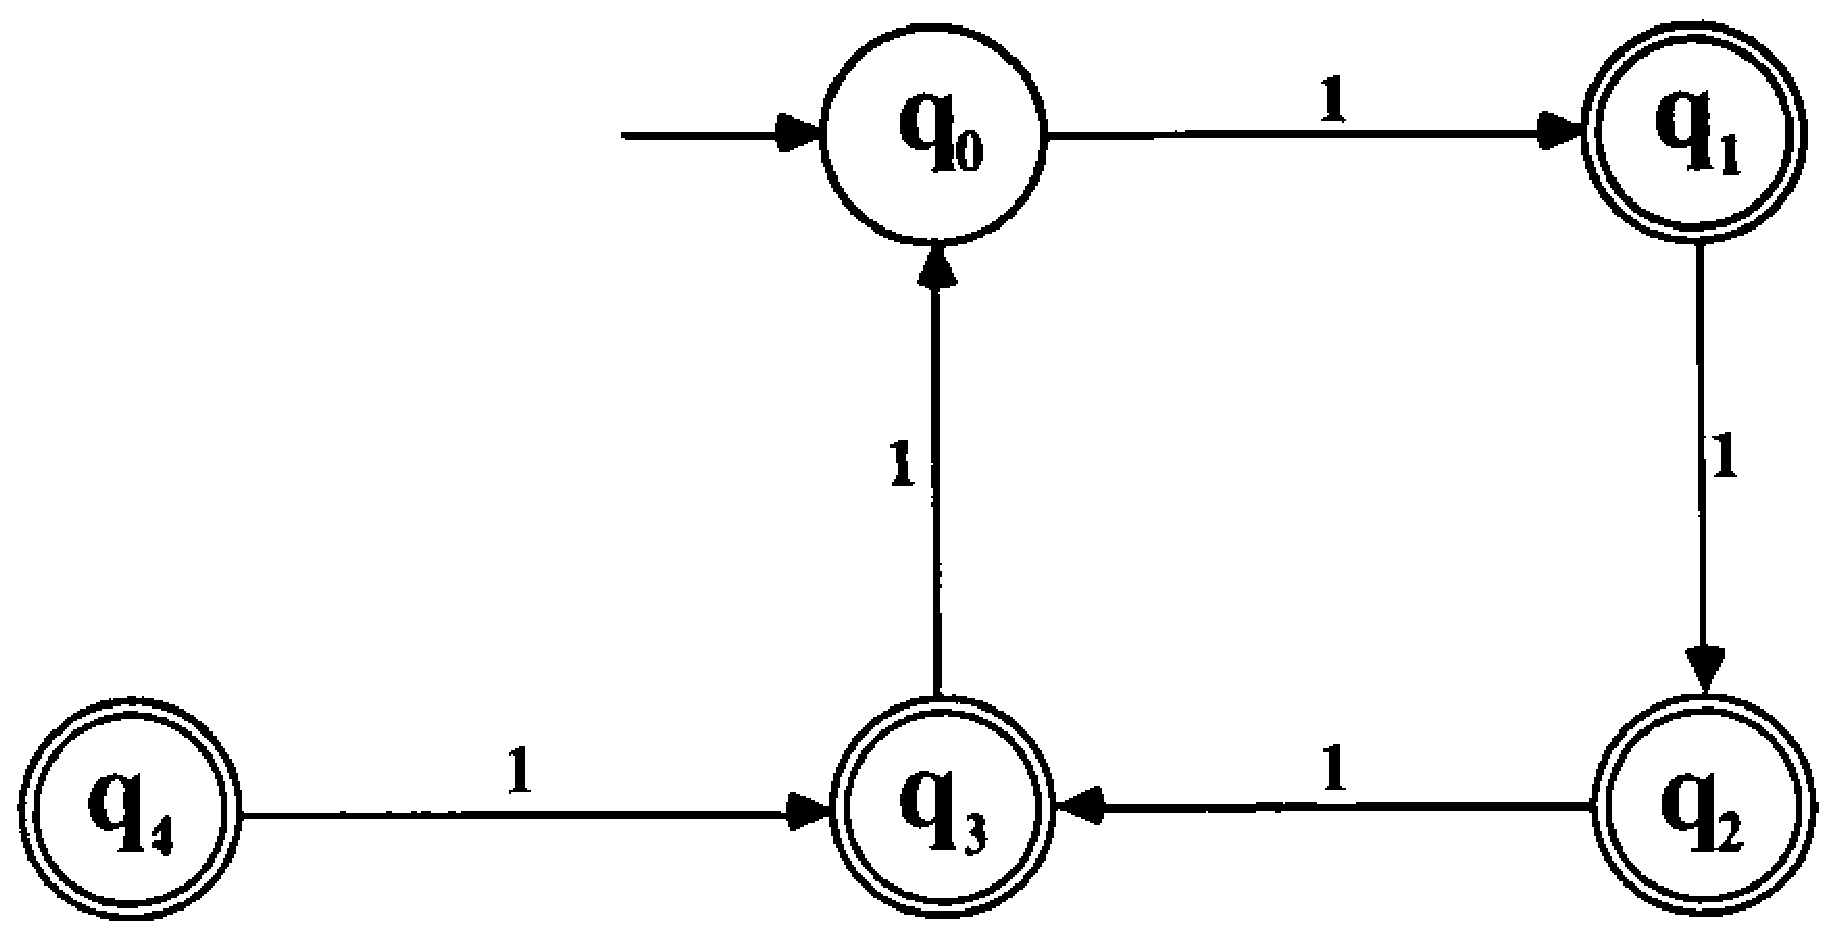
\epsfig{figure=ToFAfigures/fig3-8.eps,width=4in}}
\caption{The DFA B discussed in Example 3.14}\label{fig-3.8}
\end{figure}

The $i$th state equivalence relation provides a convenient vehicle for computing
$E_A$. The behavior exhibited by the relations in Example 3.14 follow a pattern
that is similar for all deterministic finite automata. The following
observations will culminate in a proof that the calculation of successive
partial state equivalence relations is guaranteed to lead to the relation $E_A$.

Given an integer $i$ and a finite alphabet $\Sigma$, there is clearly an
\emph{algorithm} for finding $E_{iA}$ since there are only a finite number of
strings in $\Sigma^0 \cup \Sigma^1 \cup \Sigma^2 \cup \cdots \cup \Sigma^i$.
Furthermore, given every $E_{iA}$, there is an expression for $E_A$:
$$ E_A = E_{0A} \cap E_{1A} \cap E_{2A} \cap E_{3A} \cap \cdots \cap E_{nA} \cap
	\cdots = \bigcap\limits^\infty_{j=0} E_{jA} $$
The proof is relegated to the exercises and is related to the fact that
$$ \Sigma^*=\Sigma^0\cup\Sigma^1\cup\Sigma^2\cup\cdots\cup\Sigma^n\cup\cdots $$
Finally, it should be clear that if two states cannot be distinguished by
strings of length 7 or less, they cannot be distinguished by strings of length 6
or less, which means $E_{7A}$ is a refinement of $E_{6A}$. This principle
generalizes, as formalized below.

% Lemma 3.1
\begin{lmm}\label{lmm-3.1}
Given a finite automaton $A =\langle\Sigma,S,s_0,\delta,F\rangle$ and an integer
$m$, $E_{m+1A}$ is a refinement of $E_{mA}$, which means
$$ (\forall s,t \in S)(s E_{m+1A}t \Rightarrow s E_{mA}t) $$
or
$$ E_{m+1A} \subseteq E_{mA} $$
\emph{Proof.} See the exercises.
\end{lmm}

Lemma \ref{lmm-3.2} shows that each $E_{mA}$ is related to the desired $E_A$. Lemma \ref{lmm-3.1}
thus shows that successive $E_{mA}$ relations come closer to ``looking like''
$E_A$.

% Lemma 3.2
\begin{lmm}\label{lmm-3.2}
Given a finite automaton $A =\langle\Sigma,S,s_0,\delta,F\rangle$ and an integer
$m$, $E_A$ is a refinement of $E_{mA}$, and so
$$ (\forall s,t \in S)(s E_A t \Rightarrow s E_{mA} t) $$
That is,
$$ E_A \subseteq E_{mA} $$

\emph{Proof.} Let $s,t \in S$. Then
\begin{center}
\begin{tabular}{rcl}
$s E_A t$ & $\Rightarrow$ & (by definition of $E_A$) \\
$(\forall x \in \Sigma^*)(\DBAR(s,x) \in F \Leftrightarrow \DBAR(t,x) \in F)$ &
  $\Rightarrow$ & (true for all $x$, so it is true for all ``short'' $x$)\\
$(\forall x \in \Sigma^* \ni |x| \leq m)(\DBAR(s,x) \in F \Leftrightarrow
\DBAR(t,x) \in F)$ & $\Rightarrow$ & (by definition of $E_{mA}$) \\
$s E_{mA} t$
\end{tabular}
\end{center}
\end{lmm}

While it is clearly possible to find a given $E_{mA}$ by applying the definition
to each of the strings in $\Sigma^0 \cup \Sigma^1 \cup \Sigma^2 \cup \cdots
\Sigma^m$, there is a much more efficient way if $E_{m-1A}$ is already known, as
outlined in Theorem \ref{thm-3.8}. A starting point is provided by $E_{0A}$, which can be
found very easily, as shown by Lemma \ref{lmm-3.3}. From $E_{0A}$, $E_{1A}$ can then be
found using Theorem \ref{thm-3.8}, and then $E_{2A}$, and so on.

% Lemma 3.3
\begin{lmm}\label{lmm-3.3}
Given a finite automaton $A=\langle\Sigma,S,s_0,\delta,F\rangle$, $E_{0A}$ has
two equivalence classes, $F$ and $S-F$ (unless either $F$ or $S-F$ is empty, in
which case there is only one equivalence class, $S$).

\emph{Proof.} The proof follows immediately from the definition of $E_{0A}$; the
empty string $\lambda$ differentiates between final and nonfinal states,
producing the equivalence classes outlined above.
\end{lmm}

Given $E_{0A}$ as a starting point, Theorem \ref{thm-3.8} shows how successive relations
can be efficiently calculated.

% Theorem 3.8
\begin{thm}\label{thm-3.8}
Given a finite automaton $A =\langle\Sigma,S,s_0,\delta,F\rangle$,
$$(\forall s\in S)(\forall t\in S)(\forall i \in\NN)(s E_{i+1A} t\Leftrightarrow
s E_{iA} t \wedge (\forall \pmb{a} \in \Sigma)(\delta(s,\pmb{a})E_{iA}\delta(t,\pmb{a}))) $$

\emph{Proof.} Let $s \in S,\ t \in S$. Then
\begin{center}
\begin{tabular}{rcl}
$s E_{i+1A} t$ & $\Leftrightarrow$ & $(\forall x \in \Sigma^* \ni |x| \leq i+1)
(\DBAR(s,x) \in F \Leftrightarrow \DBAR(t,x) \in F)$ \\
& $\Leftrightarrow$ & $(\forall x \in \Sigma^* \ni |x| \leq i)[\DBAR(s,x) \in F
\Leftrightarrow \DBAR(t,x) \in F] \wedge$ \\
&& $(\forall y \in \Sigma^* \ni |y| = i+1)[\DBAR(s,y) \in F \Leftrightarrow
\DBAR(t,y) \in F]$ \\
& $\Leftrightarrow$ & $(\forall x \in \Sigma^* \ni |x| \leq i)[\DBAR(s,x) \in F
\Leftrightarrow \DBAR(t,x) \in F] \wedge$ \\
&& $(\forall y \in \Sigma^* \ni 1 \leq |y| \leq i+1)[\DBAR(s,y)\in F
\Leftrightarrow \DBAR(t,y)\in F]$ \\
& $\Leftrightarrow$ & $(\forall x \in \Sigma^* \ni |x| \leq i)[\DBAR(s,x) \in F
\Leftrightarrow \DBAR(t,x) \in F] \wedge$ \\
&& $(\forall \pmb{a} \in \Sigma)(\forall x \in \Sigma^* \ni |x| \leq i)[\DBAR(s,\pmb{a}x)
\in F \Leftrightarrow \DBAR(t,\pmb{a}x) \in F]$ \\
& $\Leftrightarrow$ & $s E_{iA} t \wedge$ \\
&& $(\forall \pmb{a} \in \Sigma)(\forall x \in \Sigma^* \ni |x| \leq i)(\DBAR(s,\pmb{a}x)
\in F \Leftrightarrow \DBAR(t,\pmb{a}x) \in F)$ \\
& $\Leftrightarrow$ & $s E_{iA} t \wedge$ \\
&& $(\forall \pmb{a} \in \Sigma)(\forall x \in \Sigma^* \ni |x| \leq i)
(\DBAR(\delta(s,\pmb{a}),x) \in F \Leftrightarrow \DBAR(\delta(t,\pmb{a})x) \in F)$ \\
& $\Leftrightarrow$ & $s E_{iA} t \wedge (\forall \pmb{a} \in \Sigma)(\delta(s,\pmb{a})
E_{iA} \delta(t,\pmb{a}))$
\end{tabular}
\end{center}
\end{thm}

Note that Theorem \ref{thm-3.8} gives a far superior method for determining successive
$E_{iA}$ relations. The definition required the examination of many (long)
\emph{strings} using the $\DBAR$ function; Theorem \ref{thm-3.8} allows us to simply check
a few \emph{letters} using the $\delta$ function, without needing $\DBAR$ at all. Theorems \ref{thm-3.9},
\ref{thm-3.10}, and \ref{thm-3.11} will assure us that $E_A$ will eventually be
found. The following theorem guarantees that the relations, should they ever
begin to look alike, will continue to look alike as successive relations are
computed.

% Theorem 3.9
\begin{thm}\label{thm-3.9}
Given a finite automaton $A =\langle\Sigma,S,s_0,\delta,F\rangle$,
$$ (\exists m \in \NN \ni E_{mA} = E_{m+1A}) \Rightarrow
	(\forall k \in \NN)(E_{m+kA} = E_{mA}) $$

\emph{Proof.} By induction on $k$; see the exercises.
\end{thm}

The result in Theorem \ref{thm-3.9} is essential to the proof of the next
theorem, which guarantees that when successive relations look alike they are
identical to $E_A$.

% Theorem 3.10
\begin{thm}\label{thm-3.10}
Given a finite automaton $A =\langle\Sigma,S,s_0,\delta,F\rangle$,
$$ (\exists m \in \NN \ni E_{mA}=E_{m+1A}) \Rightarrow E_{mA}=E_A $$

\emph{Proof.} Assume $\exists m \in \NN \ni E_{mA}=E_{m+1A}$ and let
$q,r \in S$:
\begin{enumerate}
\item By Lemma \ref{lmm-3.2}, $q E_A r \Rightarrow q E_{mA} r$.
\item Conversely, assume $q E_{mA} r$. Then
\begin{center}
\begin{tabular}{rl}
$q E_{mA}r$ & $\Rightarrow$ (by assumption) \\
$q E_{m+lA} r$ & $\Rightarrow$ (by Theorem \ref{thm-3.9}) \\
$(\forall j \geq m)(q E_{jA} r)$ &
\end{tabular}
\end{center}
Furthermore, by Lemma \ref{lmm-3.1}, $(\forall j \leq m)(q E_{jA} r)$, and so
$(\forall j \in \NN)(q E_{jA} r)$; but by definition or $E_A$, this implies
$q E_A r$. We have just shown that $q E_{mA} r \Rightarrow q E_A r$.
\item Combining (1) and (2), we have
$(\forall q,r \in S)(q E_{mA} r \Leftrightarrow q E_A r)$, and so $E_{mA}=E_A$.
\end{enumerate}
\end{thm}

The next theorem guarantees that these relations \emph{will} eventually look alike
(and so by Theorem \ref{thm-3.10}, we are assured that successive computations of $E_{iA}$
will yield an expression representing the relation $E_A$).

% Theorem 3.11
\begin{thm}\label{thm-3.11}
Given a finite automaton $A =\langle\Sigma,S,s_0,\delta,F\rangle$,
$$(\exists m \in \NN \ni m \leq \|S\| \wedge E_{mA}=E_{m+1A}).$$

\emph{Proof.} Assume the conclusion is false; that is, that
$E_{0A},E_{1A}, \ldots ,E_{\|S\|A}$ are all distinct. Since
$E_{\|S\|A} \subseteq \cdots \subseteq E_{1A} \subseteq E_{0A}$, the only way
for two successive relations to be different is for the number of equivalence
classes to increase. Thus,
$$ 0 < rk(E_{0A}) < rk(E_{1A}) < rk(E_{2A}) < \cdots < rk(E_{\|S\|A}), $$
which means that $rk(E_{\|S\|A}) > \|S\|$, which is a contradiction (why?).
Therefore, not all these relations can be distinct, and so there is some index
$m$ for which $E_{mA} = E_{m+1A}$.
\end{thm}

% Corollary 3.5
\begin{cor}\label{cor-3.5}
Given a DFA $A=\langle\Sigma,S,s_0,\delta,F\rangle$, there is an \emph{algorithm} for
computing $E_A$.

\emph{Proof.} $E_A$ can be found by using Lemma \ref{lmm-3.2} to find $E_{0A}$, and
computing successive $E_{iA}$ relations using Theorem \ref{thm-3.8} until
$E_{iA}=E_{i+1A}$; this $E_{iA}$ will equal $E_A$, and this will all happen
before $i$ reaches $\|S\|$, the number of states in $S$. The procedure is
therefore guaranteed to halt.
\end{cor}

Since $E_A$ was the key to producing a reduced machine, we now have an algorithm
for taking a DFA and finding an equivalent DFA that is reduced. The other
necessary step needed to find the minimal machine was to produce a connected DFA
from a given automaton. This construction hinged on the calculation of $S^c$,
the set of connected states.

The algorithm suggested by the definition of $S^c$ is by no means the most
efficient; it involves checking long strings with the $\DBAR$ function and hence
massive duplication of effort. Furthermore, the definition seems to imply that
all the strings in $\Sigma^*$ must be checked, which certainly cannot be
completed if it is done one string at a time. Theorem \ref{thm-2.7} can be used to justify
that it is unnecessary to check any strings longer than $\|S\|$ (see the
exercises). Thus $S^c = \{\DBAR(s_0,x)| |x| < \|S\|\}$. While this set, being
based on a finite number of words, justifies that there is an algorithm for
finding $S^c$ (and hence there exists an algorithm for constructing $A^c$), it
is still a very inefficient way to calculate the set of accessible states.

As with the calculation of $E_A$, there is a way to avoid using $\DBAR$ to
process long strings when computing $S^c$. In this case, a better strategy is to
begin with $s_0$ and find all the new states that can be reached from $s_0$ with
just one transition. Note that this can be done by simply examining the row of
the state transition table corresponding to $s_0$, and hence the computation can
be accomplished quite fast. Each of these new states should then be examined in
the same fashion to see if they lead to still more states, and this process can
continue until all connected states are found. A sequence of state sets is
thereby constructed, in a similar manner to the way successive partial state
equivalence relations $E_{iA}$ were built. This approach is reflected in
Definition \ref{dfn-3.10}.

% Definition 3.10
\begin{dfn}\label{dfn-3.10}\index{i\textsuperscript{th} partial state set (DFA)}
Given a finite automaton $A=\langle\Sigma,S,s_0,\delta,F\rangle$, the 
\emph{i\textsuperscript{th} partial state set $C_i$} is defined by the following rules:
Let $C_0=\{s_0\}$ and recursively define
$$C_{i+1} = C_i \ \ \cup \bigcup\limits_{q\in C_i, \pmb{a}\in\Sigma} \delta(q,\pmb{a}).$$
\end{dfn}

$C_{\|S\|}$ must equal $S^c$ (why?), and we will often arrive at the final answer
long before $\|S\|$ iterations have been calculated (see the exercises and refer
to the treatment of $E_{iA}$). It can also be proved (by induction) that $C_i$
represents the set of all states that can be reached from $s_0$ by strings of
length $i$ or less (see the exercises).

Recall that the definition of $S^c$ involved the extended state transition
function $\DBAR$. Definition \ref{dfn-3.10} instead uses the information found in the
previous iteration to avoid calculating paths for long strings. As suggested
earlier, there is an even more efficient method of calculating $C_{i+1}$ from
$C_i$, since only paths from the newly added states need be explored anew.

\subsection*{Example 3.15}

Consider the DFA $D$ given in Figure \ref{fig-3.9}.
$$ C_0= \{s_0\} $$
and since $\delta(s_0,\pmb{a}) = s_1$, and $\delta(s_0,\pmb{b}) = s_3$,
$$ C_1 =\{s_0,s_1,s_3\} $$
Note that there is no need to check $s_0$ again, but $s_1$ and $s_3$ generate
$$ C_2 = \{s_0,s_1,s_3,s_2,s_4\} $$
Checking these two new states generates one more state, so
$$ C_3=\{s_0,s_1,s_3,s_2,s_4,s_5\} $$
and since $s_5$ leads to no new states, we have $C_4=C_3$; as with $E_{iA}$, we
will now find $C_3=C_4=C_5=C_6=\cdots=S^c$. The exercises will develop the
parallels between the generation of the partial state sets $C_i$ and the
generation of the partial state equivalence relations $E_{iA}$.

% Figure 3.9
\begin{figure}
\centerline{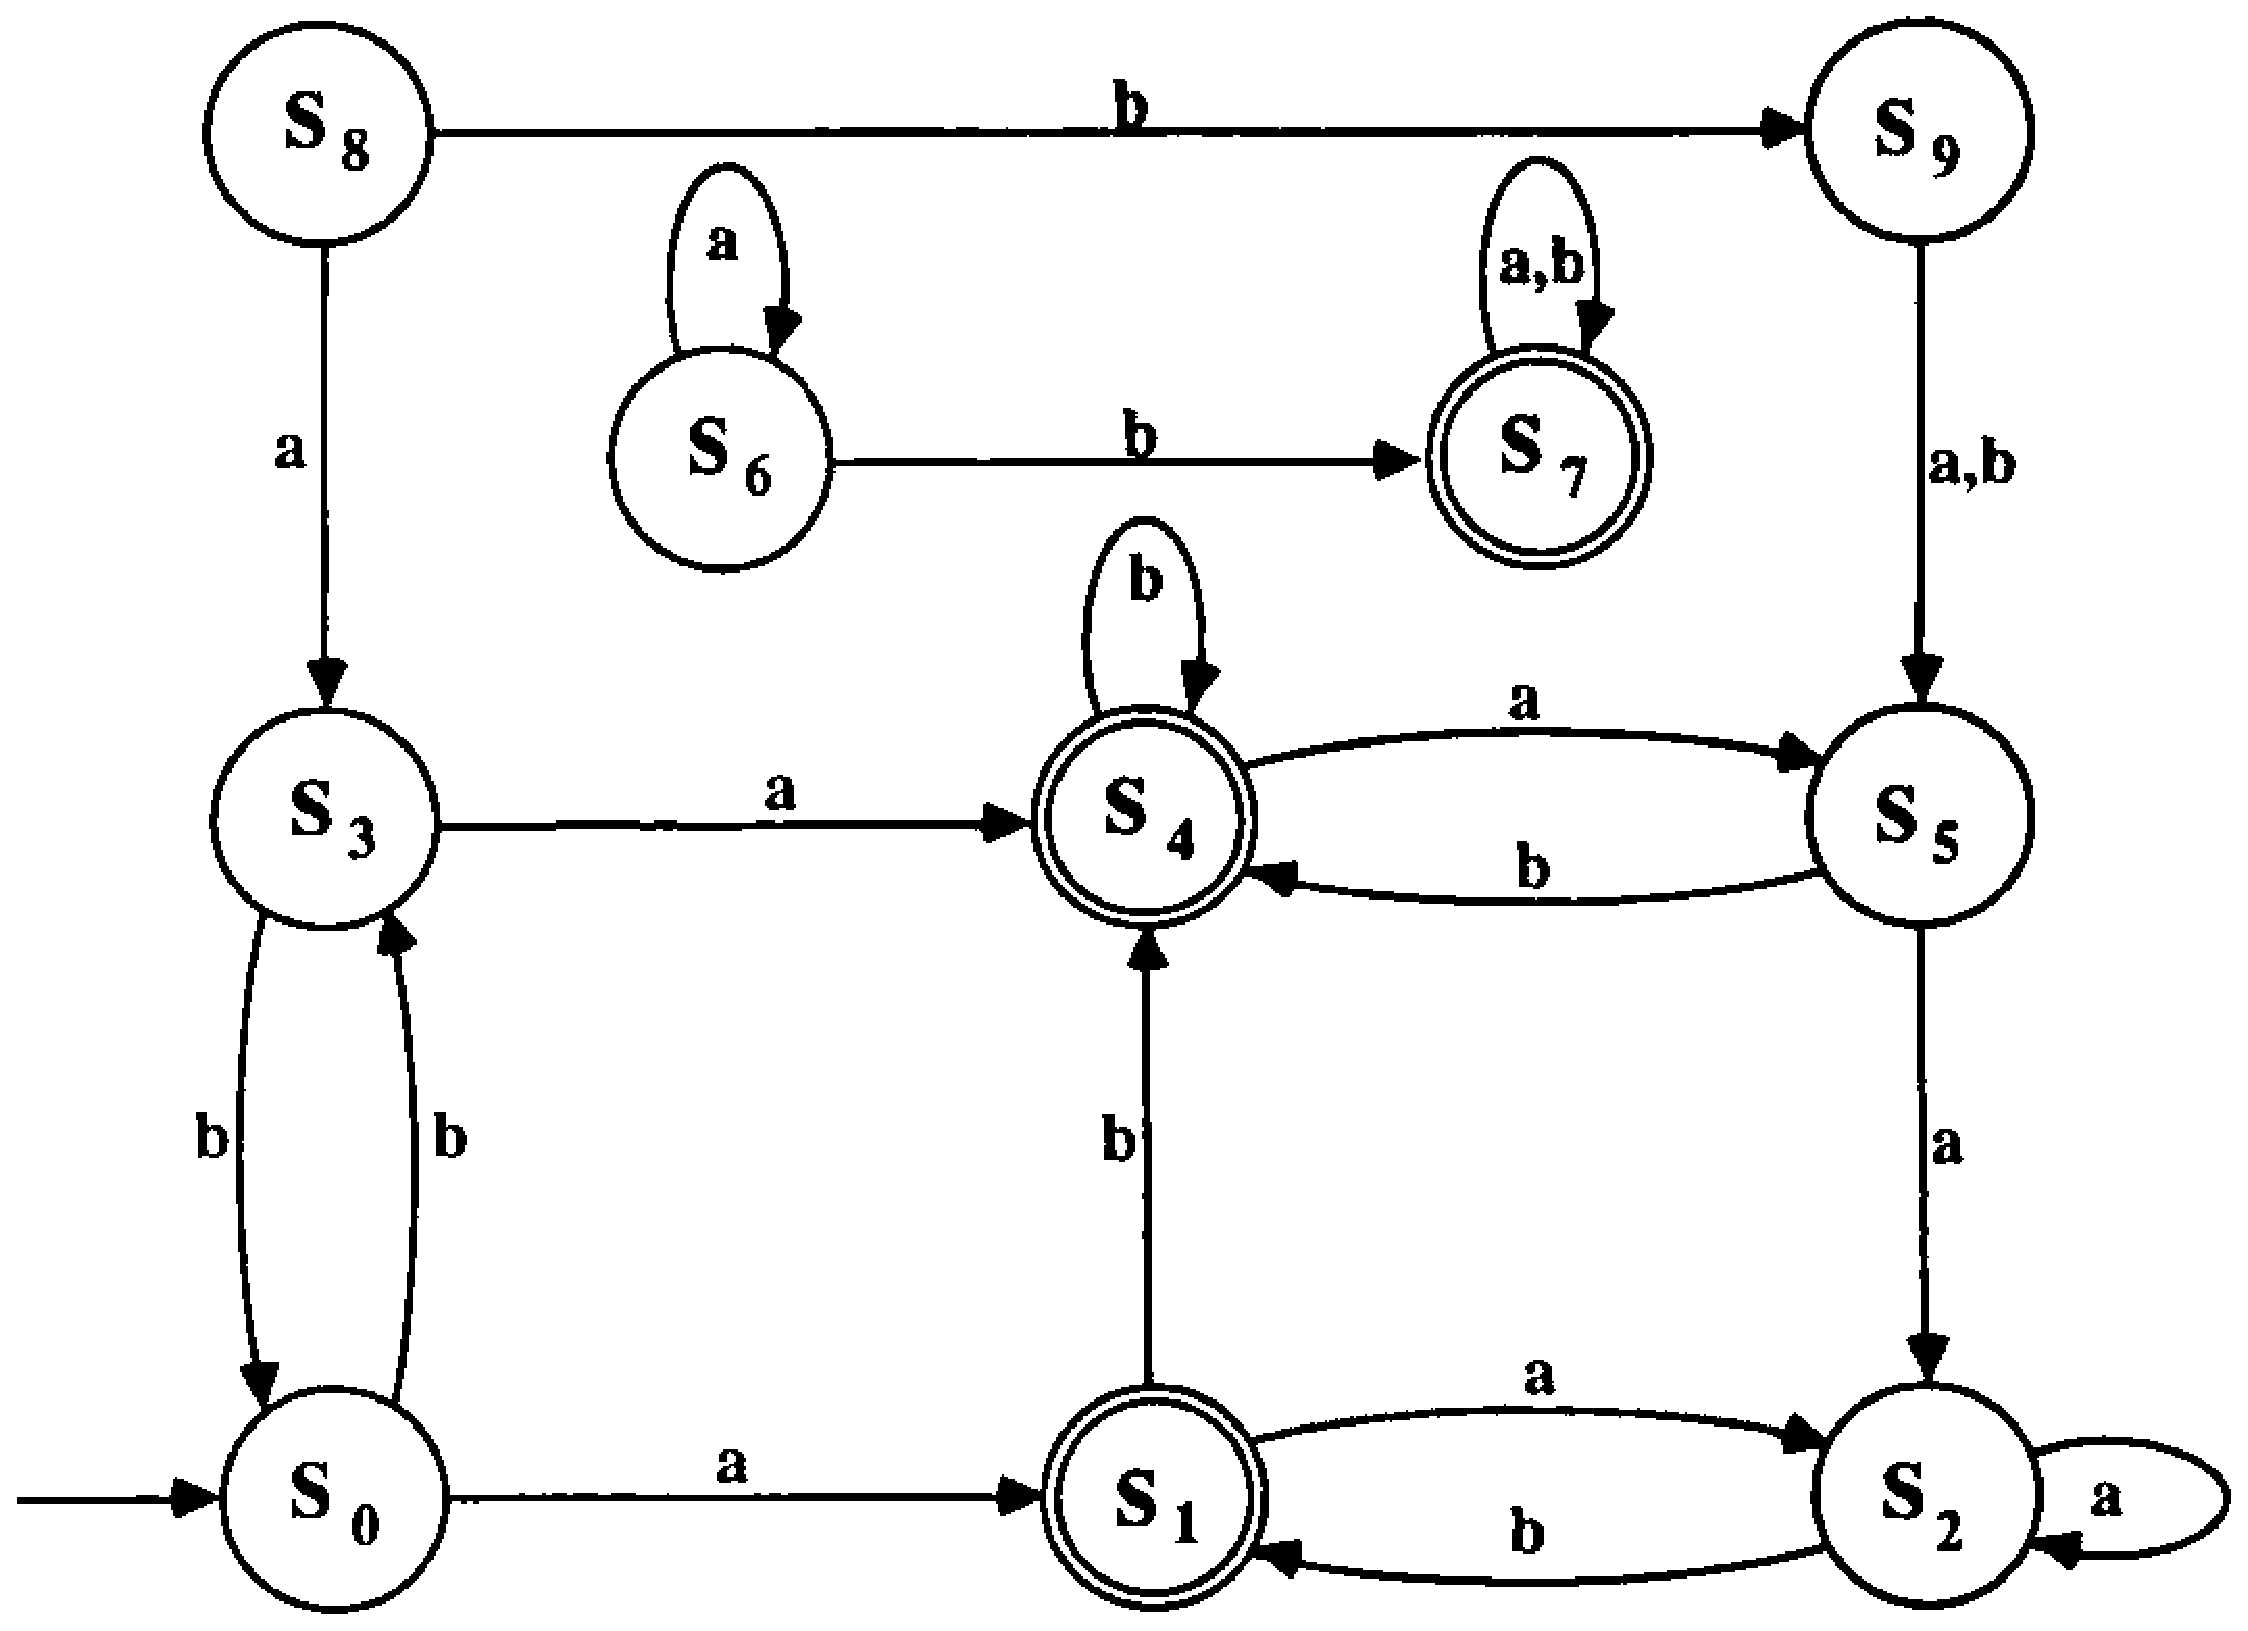
\epsfig{figure=ToFAfigures/fig3-9.eps,width=4.5in}}
\caption{The DFA D discussed in Example 3.15}\label{fig-3.9}
\end{figure}

The procedure for recursively calculating successive $C_i$s to determine $S^c$ provides
the final algorithm needed to efficiently find the minimal machine corresponding
to a given automaton $A$. From $A$, we use the $C_i$s to calculate $S^c$ and
thereby define $A^c$. Theorems \ref{thm-3.8} and related results suggest an
efficient algorithm for computing $E_A$ from which we can construct $A^c/_{E_{
A^c}}$. $A^c/_{E_{A^c}}$, is indeed the minimal machine equivalent to $A$, as
shown by the results in this chapter. Theorems \ref{thm-3.3} and \ref{thm-3.6}
show that $A^c/_{E_{A^c}}$ is equivalent to $A$. By Theorems \ref{thm-3.2},
\ref{thm-3.4}, and \ref{thm-3.5}, this automaton is reduced and connected, and
Corollary \ref{cor-3.4} guarantees that $A^c/_{E_{A^c}}$ must therefore be
minimal.

The proof of Theorem \ref{thm-3.7} suggests building a minimal equivalent deterministic
finite automaton for $A$ by first shrinking to a connected machine and then
reducing modulo the state equivalence relation, that is, by finding
$A^c/_{E_{A^c}}$. Theorem \ref{thm-3.5} assures us that when we reduce a connected machine
it will still be connected. An alternate strategy would be to first reduce
modulo $E_A$ and then shrink to a connected machine, that is, to find
$(A/_{E_A})^c$. In this case, we would want to make sure that connecting a
reduced machine will still leave us with a reduced machine. It can be shown that
if $A$ is reduced then $A^c$ is reduced (see the exercises), and hence this
method could also be used to find the minimal equivalent DFA.

Finding the minimal equivalent DFA by reducing $A$ first and then eliminating
the disconnected states is, however, less efficient than applying the algorithms
in the opposite order. Finding the connected set of states is simpler than
finding the state equivalence relation, so it is best to eliminate as many
states as possible by finding $S^c$ before embarking on the more complex search
for the state equivalence relation.

It should be clear that the algorithms in this chapter are presented in
sufficient detail to easily allow them to be programmed. As suggested in Chapter
\ref{ch-1}, the final states can be represented as a set and the transition function as a
matrix. The minimization procedures would then return the minimized matrix and
new final state set.

As a practical matter then, when generating an automaton to perform a given
task, our concern can be limited to defining a machine that \emph{works}. No further
creative insight is then necessary to find the minimal machine. Once a machine
that recognizes the desired language is found (however inefficient it may be),
the minimization algorithms can then be applied to produce a machine that is
both correct and efficient.

The proof that a reduced and connected machine is the most efficient was based
on the properties of the automaton $A_{R_L}$ obtained from the right congruence
$R_L$. This can be proved without relying on the existence of $A_{R_L}$. We
close this chapter with an outline of such a proof. The details are similar to
the proofs given in Chapter \ref{ch-7} for finite-state transducers.

Theorem \ref{thm-3.3}, which was not based in any way on $R_L$, implies that a minimal
DFA must be connected. Similarly, an immediate corollary of Theorem \ref{thm-3.6} is
that a minimal DFA must be reduced. Thus, a minimal machine is forced to be both
reduced and connected. We now must justify that a reduced and connected machine
is minimal. This result will follow from Corollary \ref{cor-3.3}, which can also be proved
without relying on $A_{R_L}$. The implication ($A \cong B \Rightarrow A$ is
equivalent to $B$) is due solely to the properties of isomorphisms and is
actually true irrespective of any other hypotheses (see the exercises).
Conversely, if $A$ is equivalent to $B$, then the fact that $A$ and $B$ are both
reduced and connected allows an isomorphism to be defined from $A$ to $B$ (see
the exercises).

Corollary \ref{cor-3.3} allows us to argue that any reduced and connected automaton $A$
is isomorphic to a minimal automaton $M$, and hence $A$ has as few states as $M$
and is minimal. The argument would proceed as follows: Since $M$ is minimal, we
already know that Theorems \ref{thm-3.3} and \ref{thm-3.6} imply that $M$ is reduced and connected.
Thus, $M$ and $A$ are two reduced and connected equivalent automata, and
Corollary \ref{cor-3.3} ensures that $A \cong M$. Thus, minimal machines are exactly those
that are reduced and connected.

\section*{Exercises}
\begin{enumerate}[{3.}1. ]
\item Use induction to show $(\forall s \in S)(\forall x \in \Sigma^*)
(\mu(\DBAR(s,x))=\DBAR_{R_L}(\mu(s), x))$ for the mapping $\mu$ defined in
Theorem \ref{thm-3.1}. %Do not appeal to the results of (5) in the proof of Theorem \ref{thm-3.1}.

\item Consider the state transition function given in Definition \ref{dfn-3.8} and use
induction to show
$$ (\forall x \in \Sigma^*)(\forall[s]_{E_A} \in S_{E_A})
	(\DBAR_{E_A}([s]_{E_A},x) = [\DBAR(s,x)]_{E_A}) $$

\item Prove that
$$ E_A = E_{0A} \cap E_{1A} \cap E_{2A} \cap E_{3A} \cap \cdots \cap E_{nA} \cap
	\cdots = \bigcap\limits^\infty_{j=0} E_{jA} $$

\item Given a finite automaton $A =\langle\Sigma,S,s_0,\delta,F\rangle$, show
that the function $\delta_{E_A}$ given in Definition \ref{dfn-3.8} is well defined.

\item Given a finite automaton $A =\langle\Sigma,S,s_0,\delta,F\rangle$, show
that the set $F_{E_A}$ given in Definition \ref{dfn-3.8} is a well-defined set.

\item Show that the range of the function $\delta^c$ given in Definition \ref{dfn-3.7} is
contained in $S^c$.

\item Prove Lemma \ref{lmm-3.1}.

\item Prove Lemma \ref{lmm-3.3}.

\item Prove Theorem \ref{thm-3.9}.

\item Given a homomorphism $\mu$ from the finite automaton 
$A=\langle\Sigma,S_A,s_{0A},\delta_A,F_A\rangle$ to the DFA 
$B=\langle\Sigma,S_B,s_{0B},\delta_B,F_B\rangle$, prove by induction that
$$ (\forall s \in S_A)(\forall x \in \Sigma^*)(\mu(\DBAR_A(s,x)) =
	\DBAR_B(\mu(s),x)) $$
	
\item Given a homomorphism $\mu$ from the finite automaton
$A=\langle\Sigma,S_A,s_{0A},\delta_A,F_A\rangle$ to the DFA 
$B=\langle\Sigma,S_B,s_{0B},\delta_B,F_B\rangle$, prove that $L(A)=L(B)$. As
long as it is explicitly cited, the result of Exercise 3.10 may be used without
proof.

\item \begin{enumerate}
\item Give an example of a DFA for which $A$ is \emph{not} connected and
$A/_{E_A}$ is not connected.
\item Give an example of a DFA for which $A$ is \emph{not} connected but
$A/_{E_A}$ \emph{is} connected.
\end{enumerate}

\item Given a finite automaton $A=\langle\Sigma,S,s_0,\delta,F\rangle$ and the
state equivalence relation $E_A$, show there exists a homomorphism from $A$ to
$A/_{E_A}$.

\item Given a \emph{connected} finite automaton
$A=\langle\Sigma,S,s_0,\delta,F\rangle$, show there exists a homomorphism from
$A$ to $A_{R_L}(A)$ by:
\begin{enumerate}
\item Define a mapping $\psi$ from $A$ to $A_{R_{L(A)}}$. (No justification need
be given.)
\item Prove that your $\psi$ is well defined.
\item Prove that $\psi$ is a homomorphism.
\end{enumerate}

\item Give an example to show that there may not exist a homomorphism from $A$
to $A_{R_{L(A)}}$ if $A$ is not connected (see Exercise 3.14).

\item Give an example to show that there may still exist a homomorphism from $A$
to $A_{R_{L(A)}}$ even if $A$ is not connected (see Exercise 3.14).

\item Give an example to show that, for the relations $R$ and $R_L$ given in
Theorem \ref{thm-2.2}, there need not exist a homomorphism from $A_{R_L}$ to $A_R$.

\item $\cong$ is an equivalence relation; in Chapter \ref{ch-2} we saw some equivalence relations
were also right congruences. Comment on the appropriateness of asking whether
$\cong$ is a right congruence.

\item Is $E_A$ a right congruence? Explain your answer.

\item Prove that if $A$ is reduced then $A^c$ is reduced.

\item For a homomorphism $\mu$ from $S_A$ to $S_B$ for the two finite automata
$A=\langle\Sigma,S_A,s_{0A},\delta_A,F_A\rangle$ and
$B=\langle\Sigma,S_B,s_{0B},\delta_B,F_B\rangle$,prove
$(\forall s,t \in S_A)(\mu(s) E_B \mu(t) \Leftrightarrow s E_A t)$.

\item Let $M$ be a DFA, and let $L=L(M)$.
\begin{enumerate}
\item Define an appropriate mapping $\psi$ from $M^c$ to $A_{(R^M)}$. (No justification need
be given.)
\item Prove that your $\psi$ is well defined.
\item Prove that $\psi$ is a homomorphism.
\item Prove that $\psi$ is a bijection.
\item Argue that $M^c \cong A_{(R^M)}$.
\end{enumerate}

\item For the machine $A$ given in Figure \ref{fig-3.10}a, find:
\begin{enumerate}
\item $E_A$ (list each $E_{iA}$)
\item $L(A)$
\item $A_{R_{L(A)}}$
\item $R_{L(A)}$
\item $A/_{E_A}$
\end{enumerate}

\item For the machine $B$ given in Figure \ref{fig-3.10}b, find:
\begin{enumerate}
\item $E_B$ (list each $E_{iB}$)
\item $L(B)$
\item $A_{R_{L(B)}}$
\item $R_{L(B)}$
\item $B/_{E_B}$
\end{enumerate}
Note that your answer to part (e) might contain some disconnected states.

\item For the machine $C$ given in Figure \ref{fig-3.10}c, find:
\begin{enumerate}
\item $E_C$ (list each $E_{iC}$)
\item $L(C)$
\item $A_{R_{L(C)}}$
\item $R_{L(C)}$
\item $C/_{E_C}$
\end{enumerate}
Note that your answer to part (e) might contain some disconnected states.

\item For the machine $D$ given in Figure \ref{fig-3.10}d, find:
\begin{enumerate}
\item $E_D$ (list each $E_{iD}$)
\item $L(D)$
\item $A_{R_{L(D)}}$
\item $R_{L(D)}$
\item $D/_{E_D}$
\end{enumerate}
Note that your answer to part (e) might contain some disconnected states.

% Figure 3.10
\begin{figure}
\centerline{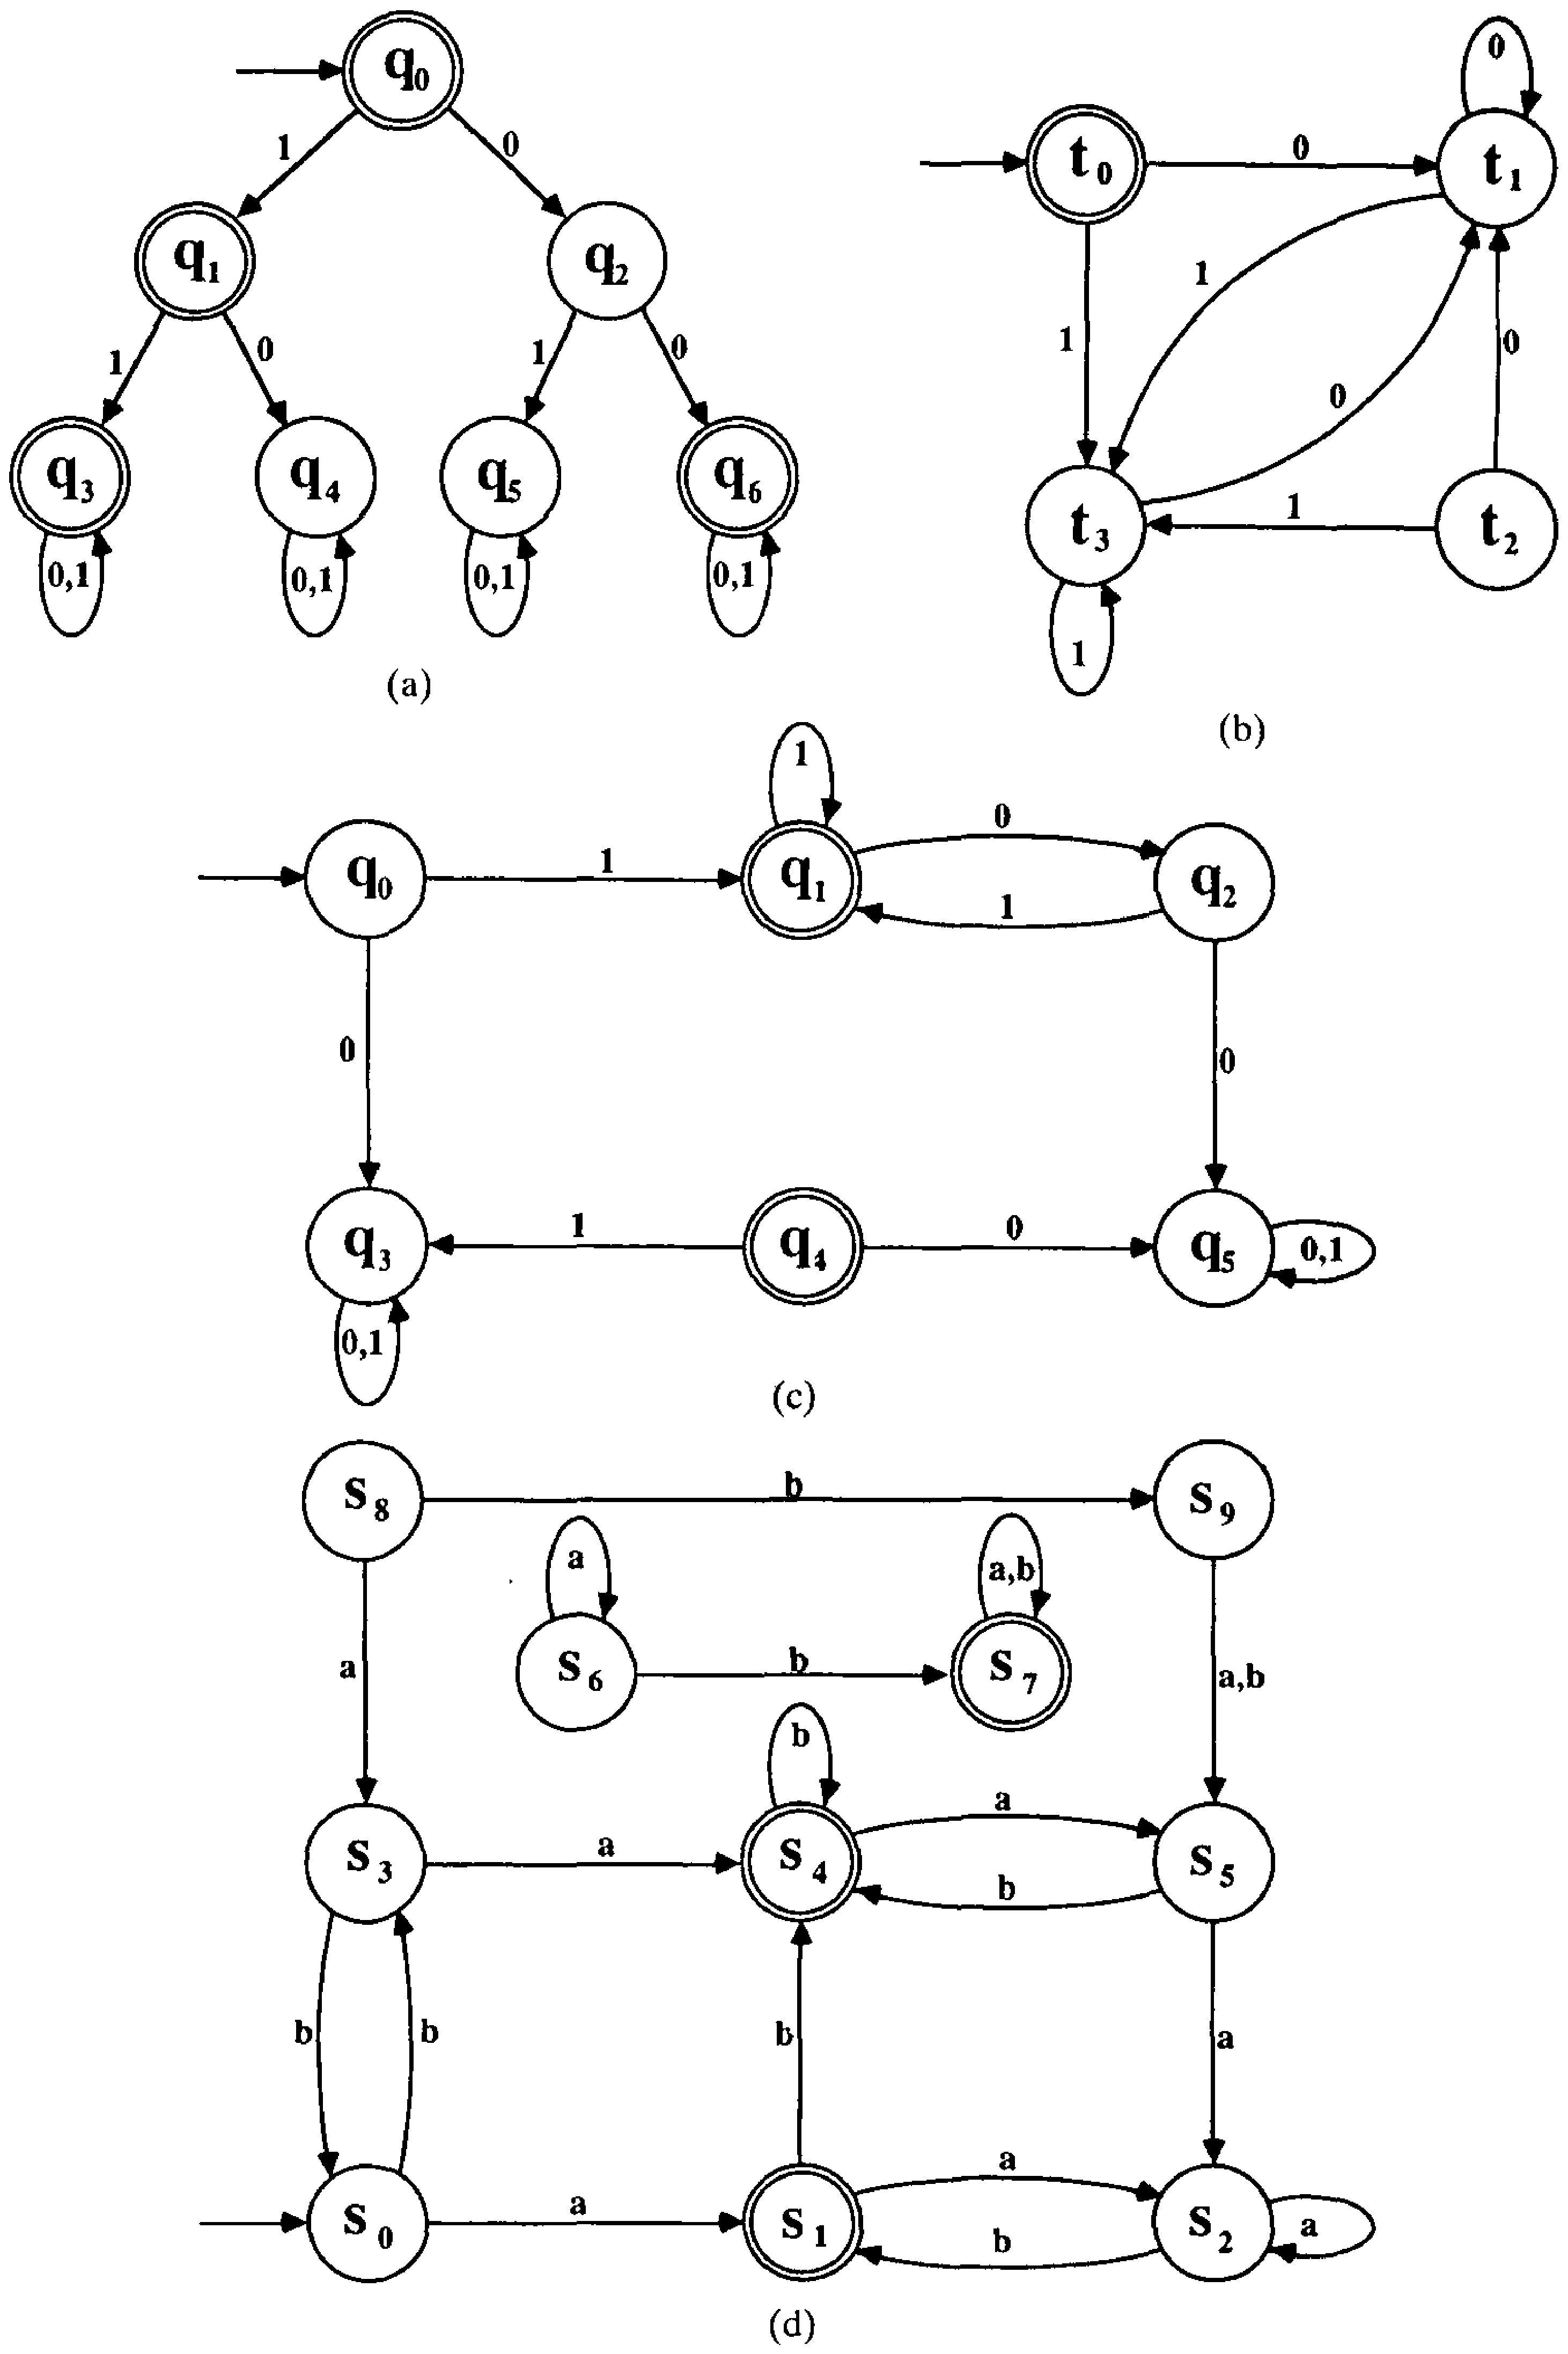
\epsfig{figure=ToFAfigures/fig3-10.eps,height=7.8in}}
\caption{(a) The DFA $A$ discussed in Exercise 3.23 (b) The DFA $B$ iscussed in
Exercise 3.24 (c) The DFA $C$ discussed in Exercise 3.25 (d) The DFA $D$
discussed in Exercise 3.26}\label{fig-3.10}
\end{figure}

\item Without relying on $A_{R_L}$, prove that if $A$ and $B$ are both reduced
and connected equivalent DFAs then $A \cong B$. Give the details for the
following steps: 
\begin{enumerate}
\item Define an appropriate function $\psi$ between the states of $A$ and the
states of $B$.
\item Show that $\psi$ is well defined.
\item Show that $\psi$ is a homomorphism.
\item Show that $\psi$ is a bijection.
\end{enumerate}

\item In the proof of (6) in Theorem \ref{thm-3.1}, the transition from line 3 to line 4 only involved
$\Rightarrow$ rather than $\Leftrightarrow$. Show by means of an example that
the two expressions involved in this transition are not equivalent.

\item Supply reasons for each of the equivalences in the proof of Theorem \ref{thm-3.8}.

\item Minimize the machine defined in Figure \ref{fig-3.3}.

\item \begin{enumerate}
\item Give an example of a DFA for which $A$ is \emph{not} reduced and $A^c$ is
not reduced.
\item Give an example of a DFA for which $A$ is \emph{not} reduced and $A^c$
\emph{is} reduced.
\end{enumerate}

\item Note that $\cong$ relates some automata to other automata, and therefore
$\cong$ is a relation over the set of all deterministic finite automata.
\begin{enumerate}
\item For automata $A,\ B$, and $C$, show that if $g$ is an isomorphism from $A$
to $B$ and $f$ is an isomorphism from $B$ to $C$, then $f \circ g$ is an
isomorphism from $A$ to $C$.
\item Prove that $\cong$ is a symmetric relation; that is, formally justify that
if there is an isomorphism from $A$ to $B$ then there is an isomorphism from $B$
to $A$.
\item Prove that $\cong$ is a reflexive relation.
\item From the results in parts (a), (b), and (c), prove that $\cong$ is an
equivalence relation over the set of all deterministic finite automata.
\end{enumerate}

\item Show that homomorphism is \emph{not} an equivalence relation over the set of
all deterministic finite automata.

\item For the relations $R$ and $R_L$ given in Theorem \ref{thm-2.2}, show that there
exists a homomorphism from $A_R$ to $A_{R_L}$.

\item Prove that if there is a homomorphism from $A$ to $B$ then $R^A$ refines
$R^B$.

\item Prove that if $A$ is isomorphic to $B$ then $R^A=R^B$
\begin{enumerate}
\item By appealing to Exercise 3.35.
\item Without appealing to Exercise 3.35.
\end{enumerate}

\item Consider two deterministic finite automata for which $A$ is not
homomorphic to $B$, but $R^A=R^B$.
\begin{enumerate}
\item Give an example of such automata for which $L(A) = L(B)$.
\item Give an example of such automata for which $L(A) \not= L(B)$.
\item Can such examples be found if both $A$ and $B$ are connected and
$L(A)=L(B)$?
\item Can such examples be found if both $A$ and $B$ are reduced and
$L(A)=L(B)$?
\end{enumerate}

\item Disprove that if $A$ is homomorphic to $B$ then $R^A=R^B$.

\item Prove or give a counterexample [assume $L = L(M)$].
\begin{enumerate}
\item For any DFA $M$, there exists a homomorphism $\psi$ from $A_{(R^M)}$ to
$M$.
\item For any DFA $M$, there exists an isomorphism $\psi$ from $A_{(R^M)}$ to
$M$.
\item For any DFA $M$, there exists a homomorphism $\psi$ from $M$ to
$A_{(R^M)}$.
\end{enumerate}

\item Prove that if $A$ is a minimal DFA then $R^A = R_{L(A)}$.

\item Give an example to show that Exercise 3.40 can be false if $A$ is not
minimal.

\item Give an example to show that Exercise 3.40 may still hold if $A$ is not
minimal.

\item Definition \ref{dfn-3.8} takes an equivalence relation of the set of states $S$ and
defines a machine based on that relation. In general, we could choose a relation
$R$ in $S$ and define a machine $A/_R$ (as we did when we defined $A/_{E_A}$
when the relation $R$ was $E_A$).
\begin{enumerate}
\item Consider $R=E_{0A}$. Is $A/_{E_{0A}}$ always well defined? Give an example
to illustrate your answer.
\item Assume $R$ is a refinement of $E_A$. Is $A/_R$ always well defined? For
the cases where it is well defined, consider the theorems that would correspond
to Theorems \ref{thm-3.4}, \ref{thm-3.5}, and \ref{thm-3.6} if $E_A$ were replaced by such a refinement $R$.
Which of these theorems would still be true?
\end{enumerate}

\item Given a DFA $M$, prove or give a counterexample.
\begin{enumerate}
\item There exists a homomorphism from $M/_{E_M}$ to $A_{R_{L(M)}}$.
\item There exists a homomorphism from $A_{R_{L(M)}}$ to $M/_{E_M}$.
\end{enumerate}

\item Prove that the bound given for Theorem \ref{thm-3.11} can be sharpened: given a
finite automaton $A=\langle\Sigma,S,s_0,\delta,F\rangle$,
$(\exists m \in \NN \ni m < \|S\| \wedge E_{mA} = E_{m+1A})$.

\item Prove or give a counterexample:
\begin{enumerate}
\item If $A$ and $B$ are equivalent, then $A$ and $B$ are isomorphic.
\item If $A$ and $B$ are isomorphic, then $A$ and $B$ are equivalent.
\end{enumerate}

\item Given a finite automaton $A =\langle\Sigma,S,s_0,\delta,F\rangle$, prove
that the $C_i$s given in Definition \ref{dfn-3.10} are nested:
$(\forall i \in \NN)(C_i \subseteq C_{i+1})$.

\item Prove (by induction) that $C_i$ does indeed represent the set of all
states that can be reached from $s_0$ by strings of length $i$ or less.

\item Prove that, given a finite automaton
$A =\langle\Sigma,S,s_0,\delta,F\rangle$,
$$ (\exists i \in \NN \ni C_i=C_{i+1}) \Rightarrow
	(\forall k \in \NN)(C_i = C_{i+k}). $$

\item Prove that, given a DFA $A =\langle\Sigma,S,s_0,\delta,F\rangle$,
$(\exists i \in \NN \ni C_i = C_{i+1}) \Rightarrow (C_i = S^c)$.

\item Prove that, given a finite automaton
$A =\langle\Sigma,S,s_0,\delta,F\rangle,\ \exists i \in \NN \ni C_i = C_{i+1}$.

\item Prove that, given a DFA $A =\langle\Sigma,S,s_0,\delta,F\rangle$,
$(\exists i \in \NN \ni i \leq \|S\| \wedge C_i = S^c)$.

\item Use the results of Exercises 3.47 through 3.52 to argue that the procedure
for generating $S^c$ from successive calculations of $C_i$ is correct and is
actually an algorithm.

\item Give an example of two DFAs $A$ and $B$ that simultaneously satisfy the
following three criteria:
\begin{enumerate}[1.]
\item There is a homomorphism from $A$ to $B$.
\item There is a homomorphism from $B$ to $A$.
\item There does not exist any isomorphism between $A$ and $B$.
\end{enumerate}

\item Assume $R$ and $Q$ are both right congruences of finite rank, $R$ refines
$Q$, and $L$ is a union of equivalence classes of $Q$.
\begin{enumerate}
\item Show that $L$ is also a union of equivalence classes of $R$.
\item Show that there exists a homomorphism from $A_R$ to $A_Q$. (\emph{Hint:}
Do \emph{not} use the $\mu$ given in Theorem \ref{thm-3.1}; there is a far more
straightforward way to define a mapping.)
\item Give an example to show that there need not be a homomorphism from $A_Q$
to $A_R$.
\end{enumerate}

\item Prove that $A_Q$ must be connected.

\item Prove that if there is an isomorphism from $A$ to $B$ and $A$ is connected
then $B$ must also be connected.

\item Prove that if there is an isomorphism from $A$ to $B$ and $B$ is connected
then $A$ must also be connected.

\item Disprove that if there is a homomorphism from $A$ to $B$ and $A$ is
connected then $B$ must also be connected.

\item Disprove that if there is a homomorphism from $A$ to $B$ and $B$ is
connected then $A$ must also be connected.

\item Given a DFA $A$, recall the relation $R^A$ on $\Sigma^*$ induced by $A$.
This relation gives rise to another DFA $A_{(R^A)}$ [with $Q=R^A$ and $L=L(A)$].
Consider also the connected version of $A$, $A^c$.
\begin{enumerate}
\item Define an isomorphism $\psi$ from $A_{(R^A)}$ to $A^c$. (No justification
need be given.)
\item Prove that your $\psi$ is well defined.
\item Prove that $\psi$ is a homomorphism.
\item Prove that $\psi$ is an isomorphism.
\end{enumerate}

\item Assume that $A$ and $B$ are connected DFAs. Assume that there exists an
isomorphism $\psi$ from $A$ to $B$ and an isomorphism $\mu$ from $B$ to $A$.
Prove that $\psi = \mu^{-1}$.

\item Assume that $A$ and $B$ are DFAs. Assume that there exists an isomorphism
$\psi$ from $A$ to $B$ and an isomorphism $\mu$ from $B$ to $A$. Give an example
for which $\psi \not= \mu^{-1}$.

\item Give an example of a three-state DFA for which $E_{0A}$ has only one
equivalence class. Is it possible for $E_{0A}$ to be different from $E_{1A}$ in
such a machine? Explain.

\item Assume A and B are both reduced and connected. If $\psi$ is a homomorphism
from $A$ to $B$, does $\psi$ have to be an isomorphism? Justify your
conclusions.

\item Prove Corollary \ref{cor-3.2}.

\item Prove that $S^c =\{\DBAR(s_0,x)|\ |x| \leq \|S\|\}$.

\item Given a finite automaton $A=\langle\Sigma,S,s_0,\delta,F\rangle$, two
states $s,t \in S$, and the automata $A^t=\langle\Sigma,S,t,\delta,F\rangle$ and
$A^s=\langle\Sigma,S,s,\delta,F\rangle$, prove that $s E_A t \Leftrightarrow
L(A^s) = L(A^t)$.

\item Given a finite automaton $A=\langle\Sigma,S,s_0,\delta,F\rangle$, consider
the terminal sets $T(A,t)=\{x$ $|$ $\DBAR(t,x) \in F\}$ and initial sets
$I(A,t)=\{x$ $|$ $\DBAR(s_0,x) = t\}$ for each $t \in S$.
\begin{enumerate}
\item Prove that the initial sets of $A$ must form a partition of $\Sigma^*$.
\item Give an example to show that the terminal sets of $A$ might not partition
$\Sigma^*$.
\item Give an example to show that the terminal sets of $A$ might partition
$\Sigma^*$.
\end{enumerate}
\end{enumerate}

\chapter{Nondeterministic Finite Automata}\label{ch-4}

A nondeterministic finite automaton, abbreviated NDFA, is a
generalization of the deterministic machines that we have studied
in previous chapters. Although nondeterministic machines lack some
of the restrictions imposed on their deterministic cousins, the
class of languages recognized by nondeterministic finite automata
is exactly the same as the class of languages recognized by
deterministic finite automata.  In this sense, the recognition power
of nondeterministic finite automata is equivalent to that of
deterministic finite automata.

In this chapter we will show the correspondence of nondeterministic
finite automata to deterministic finite automata, and we will prove
that both types of machines accept the same class of languages. In
a later section, we will again generalize our computational model
to allow nondeterministic finite automata that make transitions
spontaneously, without an input symbol being processed. It will be
shown that the class of languages recognized by these new machines
is exactly the same as the class of languages recognized by our
first type of nondeterministic finite automata and is thus the same
as the class of languages recognized by deterministic finite automata.

% 4.1 DEFINITIONS AND BASIC THEOREMS
\section{Definitions and Basic Theorems}\label{sec-4.1}

Whereas deterministic finite automata are restricted to having
exactly one transition from a state for each $\mathbf{a} \in \Sigma$, a
nondeterministic finite automaton may have any number of transitions
for a given input symbol, including zero transitions.

When processing an input string, if an NDFA comes to a state from
which there is no transition arc labeled with the next input symbol,
the path through the machine which is being followed is terminated.
Termination can take the place of the ``garbage state'' (a permanent
rejection state) found in many deterministic finite automata, which
is used to reject some strings that are not in the language recognized
by the automaton (the state $s_7$ played this role in Examples 1.11 and
1.9).

\subsection*{Example 4.1}

Let $L=\{w \in \{\pmb{a},\pmb{b},\pmb{c}\}^*|\ \exists y \in \{\pmb{b}\}^* \ni
w = \pmb{a}y\pmb{c}\}$.  We can easily build a nondeterministic finite automaton
that accepts this set of words. One such automaton is displayed in Figure \ref{fig-4.1}.
In this example there are no transitions out of $s_0$ labeled with either
$\pmb{b}$ or $\pmb{c}$, nor are there any transitions from $s_1$ labeled with
$\pmb{a}$. From state $s_2$ there are no transitions at all. This means that if
either $\pmb{b}$ or $\pmb{c}$ is encountered in state $s_0$ or $\pmb{a}$ is
encountered in state $s_1$, or any input letter is encountered once we reach
state $s_2$, the word on the input tape will not be able to follow this
particular path through the machine. Thus, if a word is not fully processed by
the NDFA, it will not be considered accepted (even if the state in which it was
prematurely ``stuck'' was a final state).

% Figure 4.1
\begin{figure}
\centerline{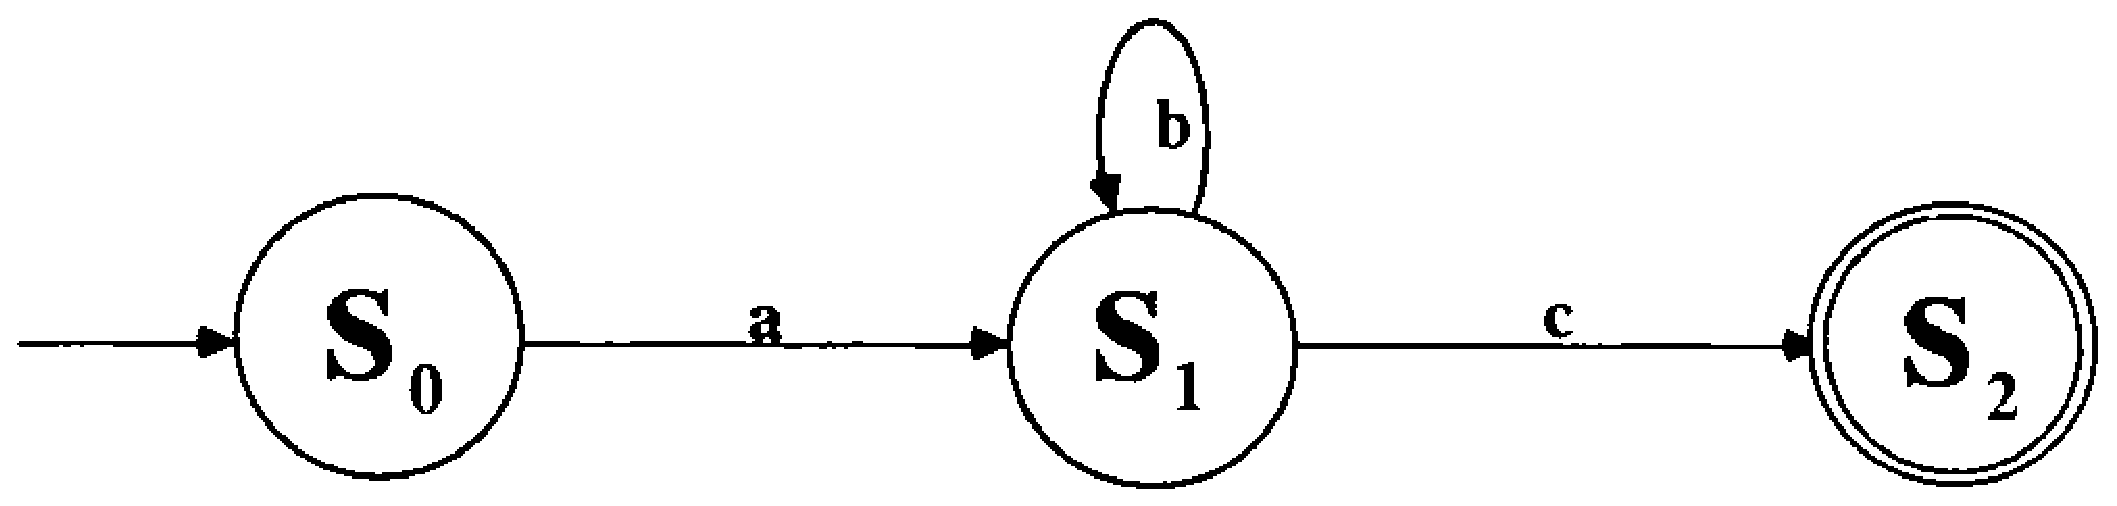
\epsfig{figure=ToFAfigures/fig4-1.eps,width=3in}}
\caption{The NDFA described in Example 4.1}\label{fig-4.1}
\end{figure}

An equivalent, although more complicated, deterministic finite automaton is
given in Figure \ref{fig-4.2}. Note that this deterministic finite automaton requires
the introduction of an extra state, a \emph{\Index{dead state}} or
\emph{\Index{garbage state}}, to continue the processing of strings that are not
in the language.

% Figure 4.2
\begin{figure}
\centerline{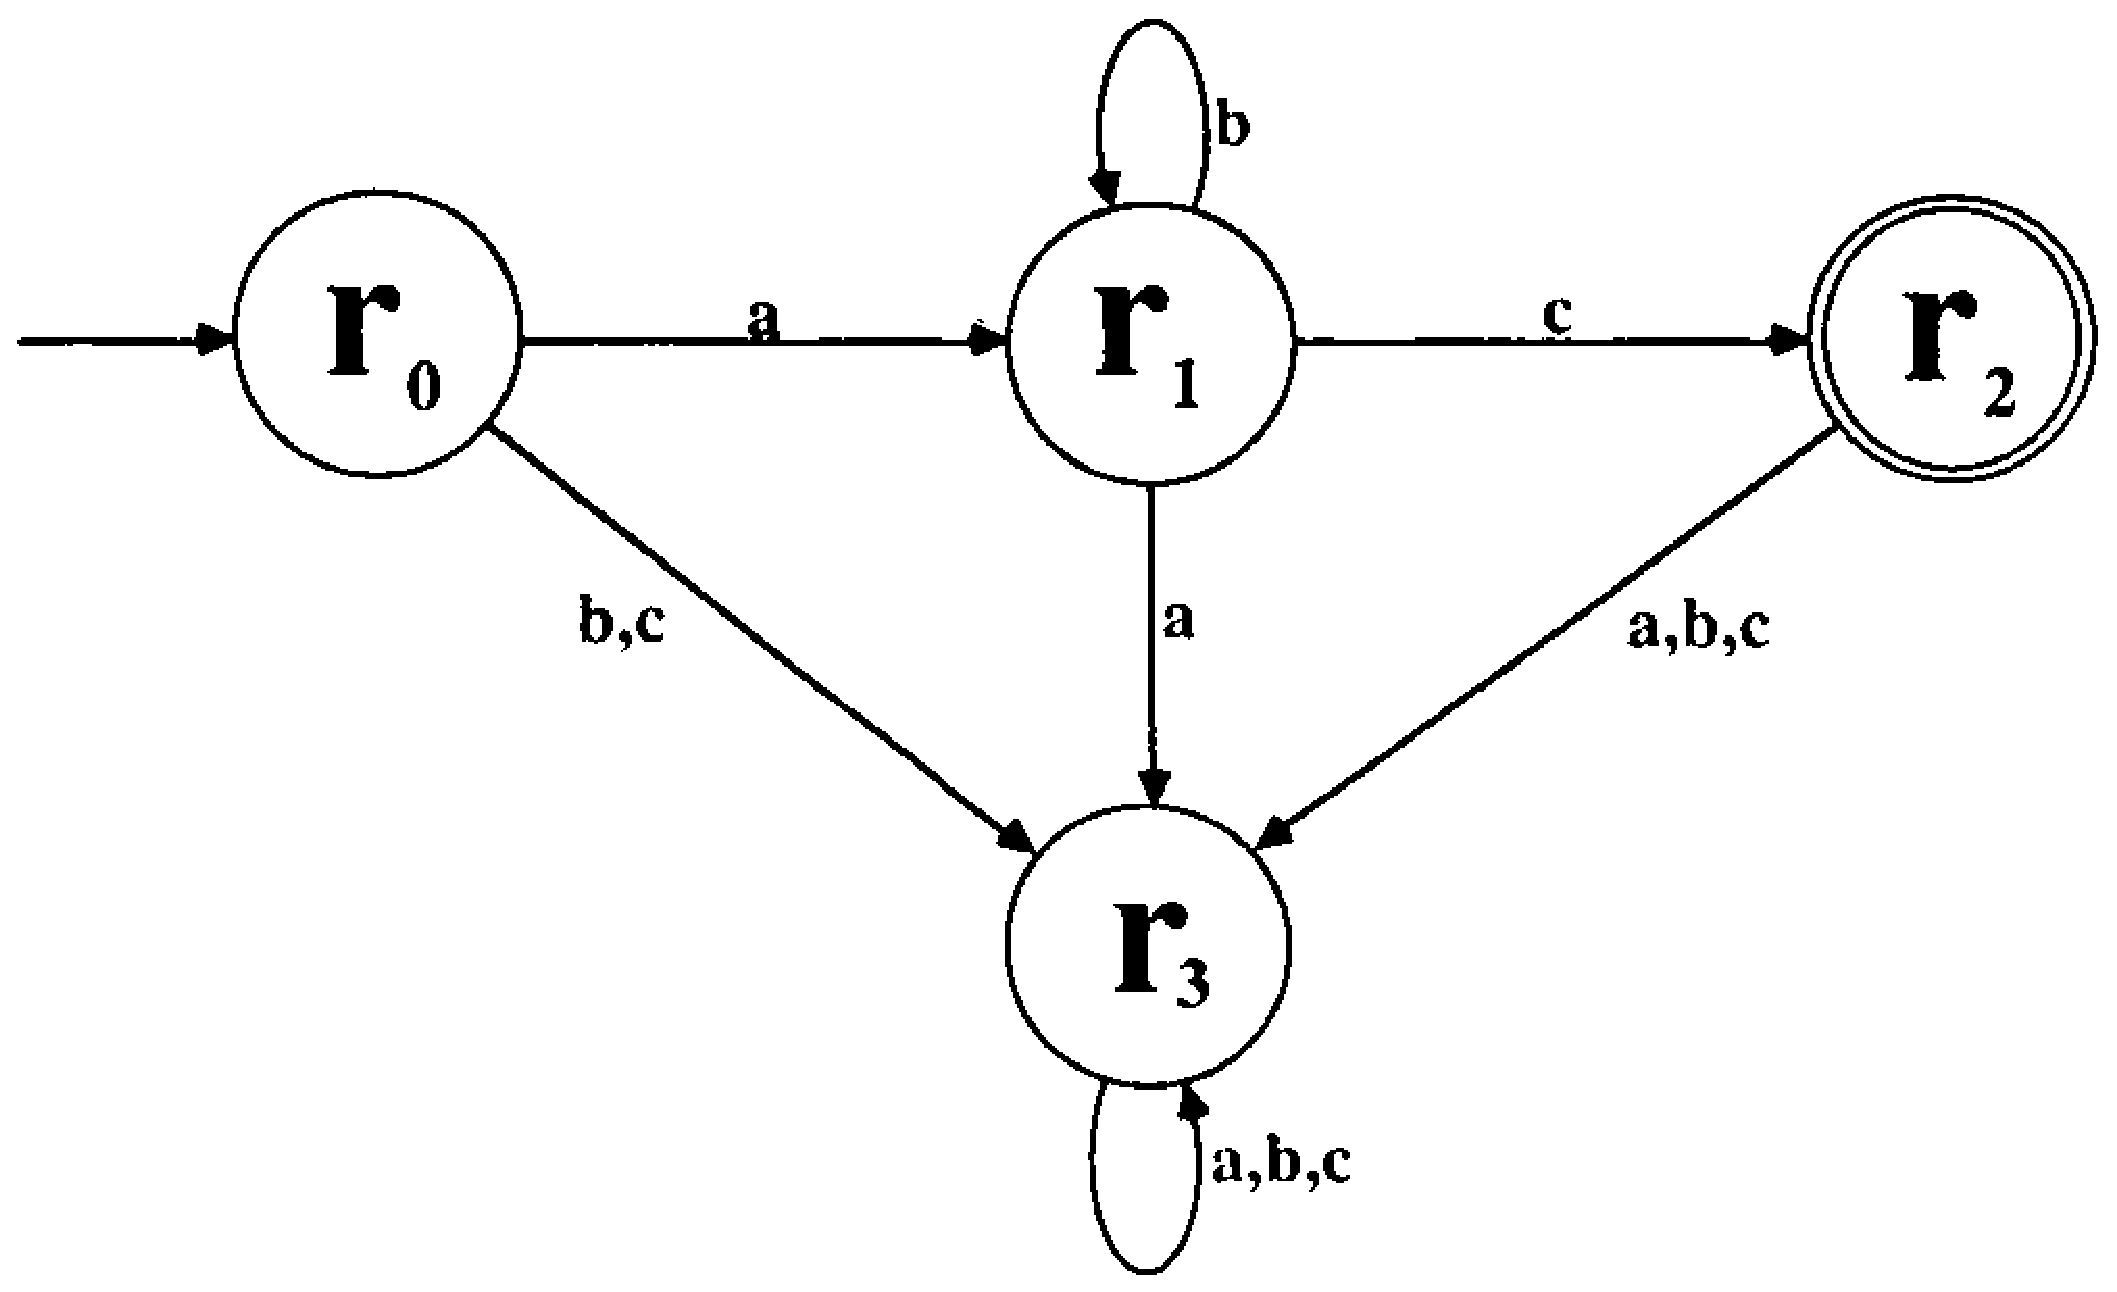
\epsfig{figure=ToFAfigures/fig4-2.eps,width=3in}}
\caption{A deterministic version of the NDFA in Example 4.1}\label{fig-4.2}
\end{figure}

A nondeterministic finite automaton may also have \emph{multiple} transitions
from any state for a given input symbol. For example, consider the following
construction of a nondeterministic acceptor for the language $L$, which consists
of all even-length strings along with all strings whose number of $\pmb{1}$s is
a multiple of 3. That is, $L=\{x \in \{\pmb{0},\pmb{1}\}^*|\ |x| \equiv 0 \bmod{2}
\vee |x|_{\pmb{1}} \equiv 0 \bmod{3}\}$.

\subsection*{Example 4.2}

In the NDFA given in Figure \ref{fig-4.3}, there are multiple transitions from state $s_0$:
processing the symbol $\pmb{0}$ causes the machine to enter states $s_1$ and
$s_2$, whereas processing a $\pmb{1}$ causes the machine to enter both state
$s_3$ and state $s_2$.

% Figure 4.3
\begin{figure}
\centerline{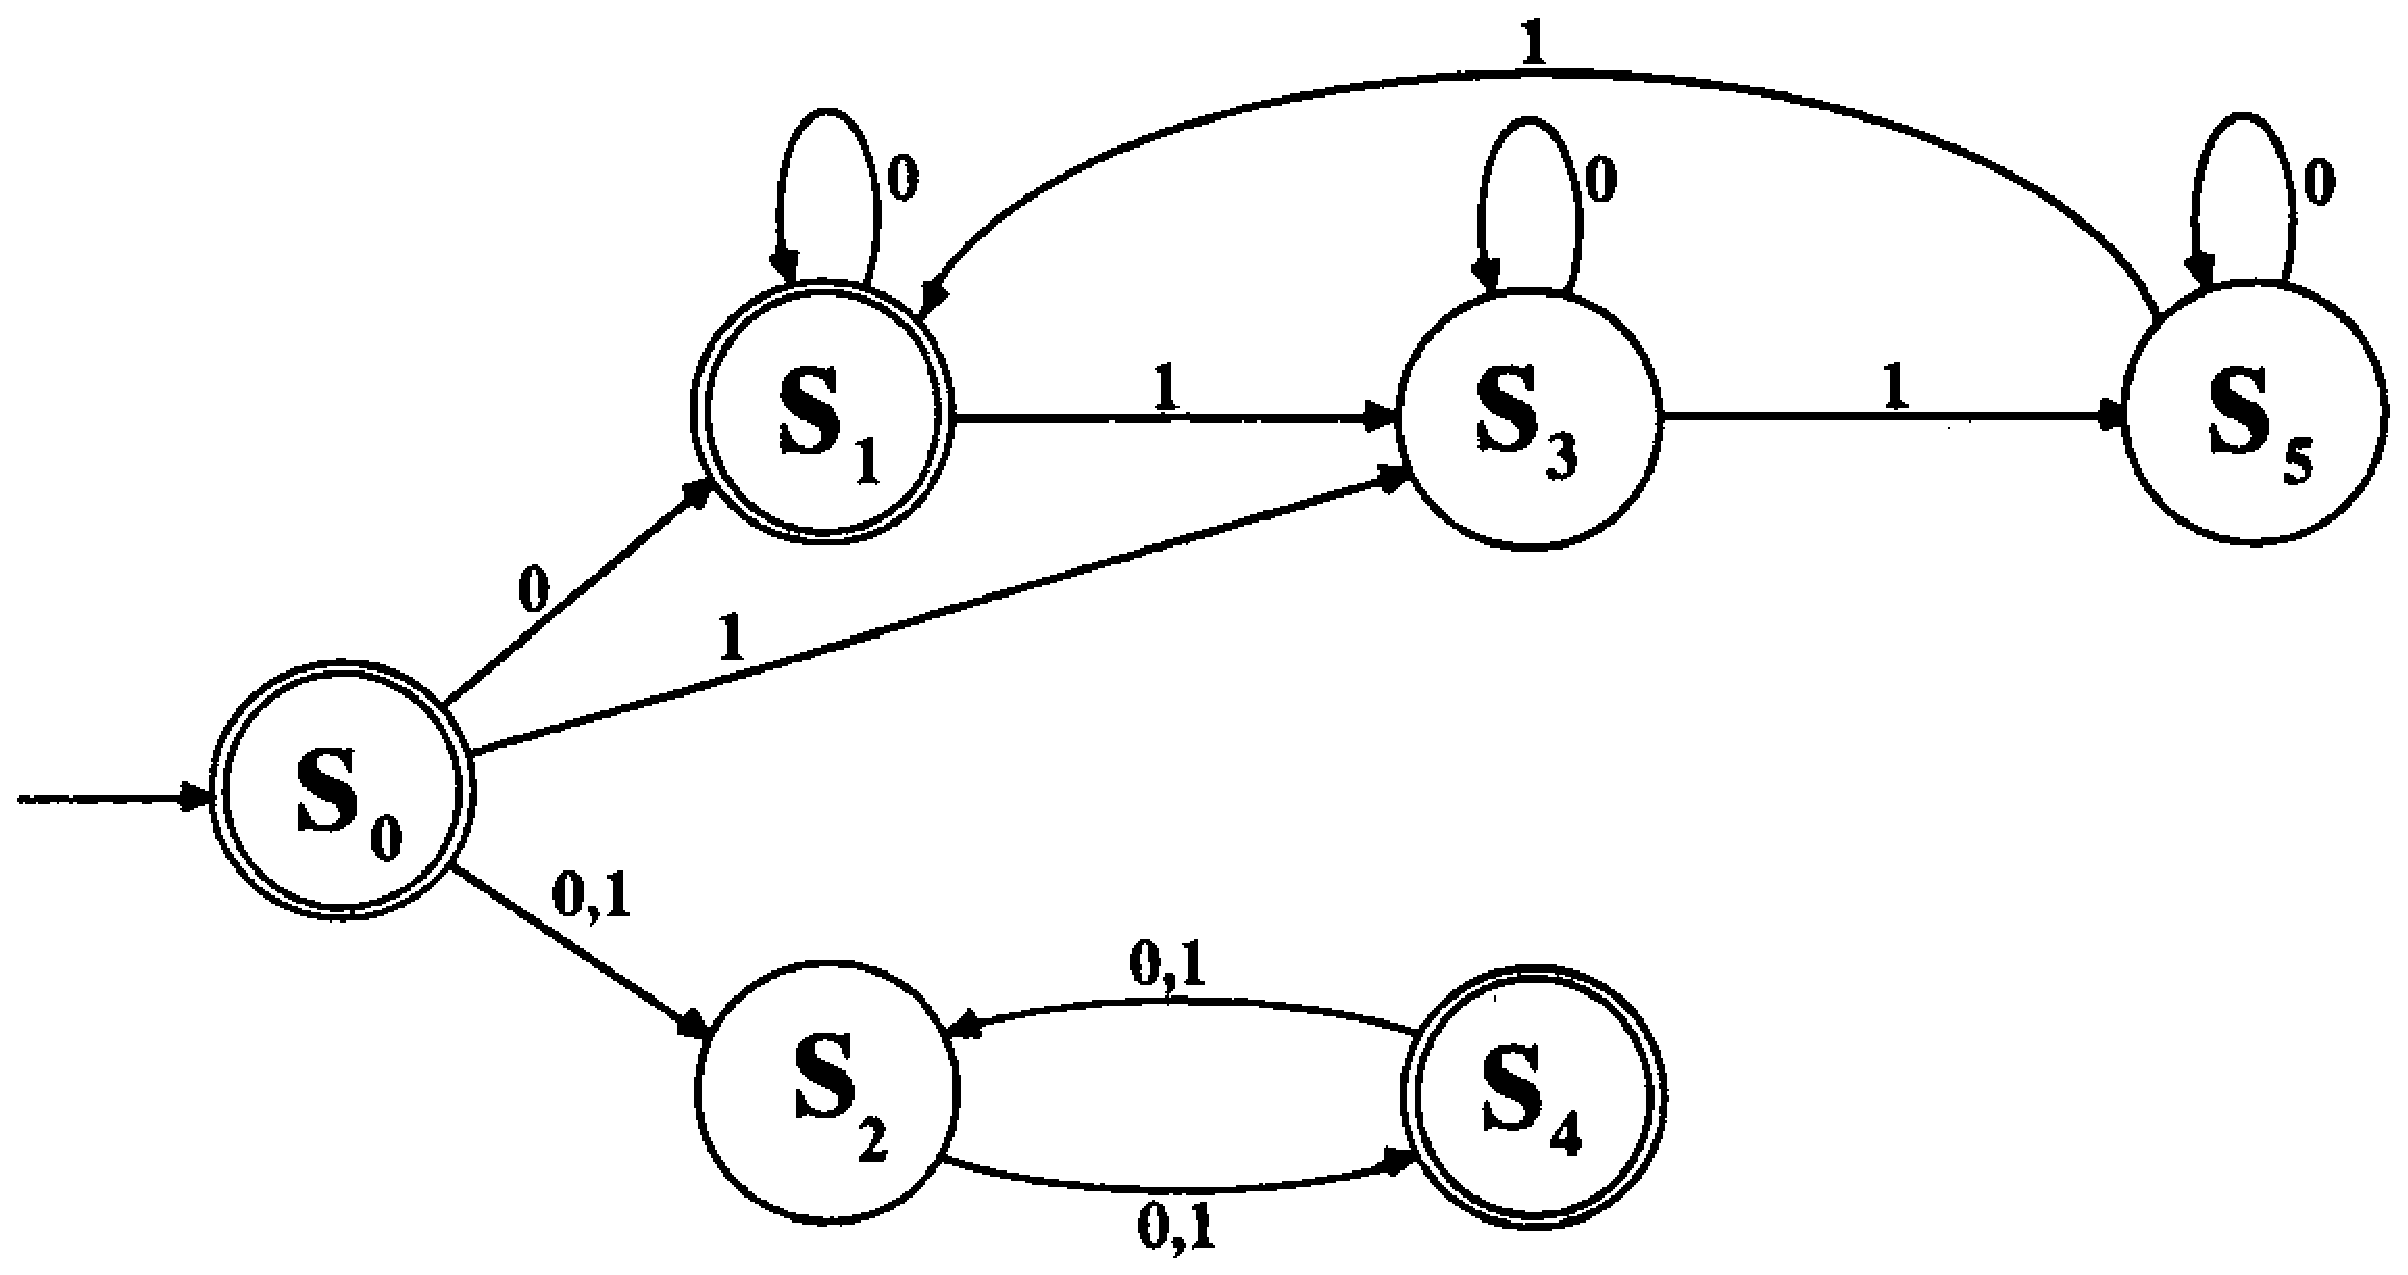
\epsfig{figure=ToFAfigures/fig4-3.eps,width=4in}}
\caption{The NDFA discussed in Example 4.2}\label{fig-4.3}
\end{figure}

Within a nondeterministic finite automaton there can be multiple paths that
are labeled with the components of a string. For example, if we let $w=\pmb{01}$,
then there are two paths labeled by the components of $w:\ (s_0 \rightarrow s_1
\rightarrow s_3)$ and $(s_0 \rightarrow s_2 \rightarrow s_4)$. The second path
leads to a final state, $s_4$, while the first path does not. We will adopt
the convention that this word $w$ \emph{is} accepted by the automaton since at
least one of the paths \emph{does} terminate in a final state. These concepts
will be formalized later in Definition \ref{dfn-4.3}.

This ability to make multiple transitions from a given state can simplify the
construction of the machine, but adds no more power to our computational model.
The deterministic machine equivalent to Example 4.2 is substantially more
complex, and its construction is left as an exercise for the reader.

Another restriction that is relaxed when we talk about nondeterministic finite
automata is the number of initial states. While a deterministic machine is
constrained to having exactly one start state, a nondeterministic finite
automaton may have any number, other than zero, up to $\|S\|$. Indeed, some
applications will be seen in which \emph{all} the states are start states.

\subsection*{Example 4.3}

We can build a machine that will accept the same language as in Example 4.2,
but in a slightly different way. Note that in Figure \ref{fig-4.4} the multiplicity of
start states simplifies the construction considerably.

% Figure 4.4
\begin{figure}
\centerline{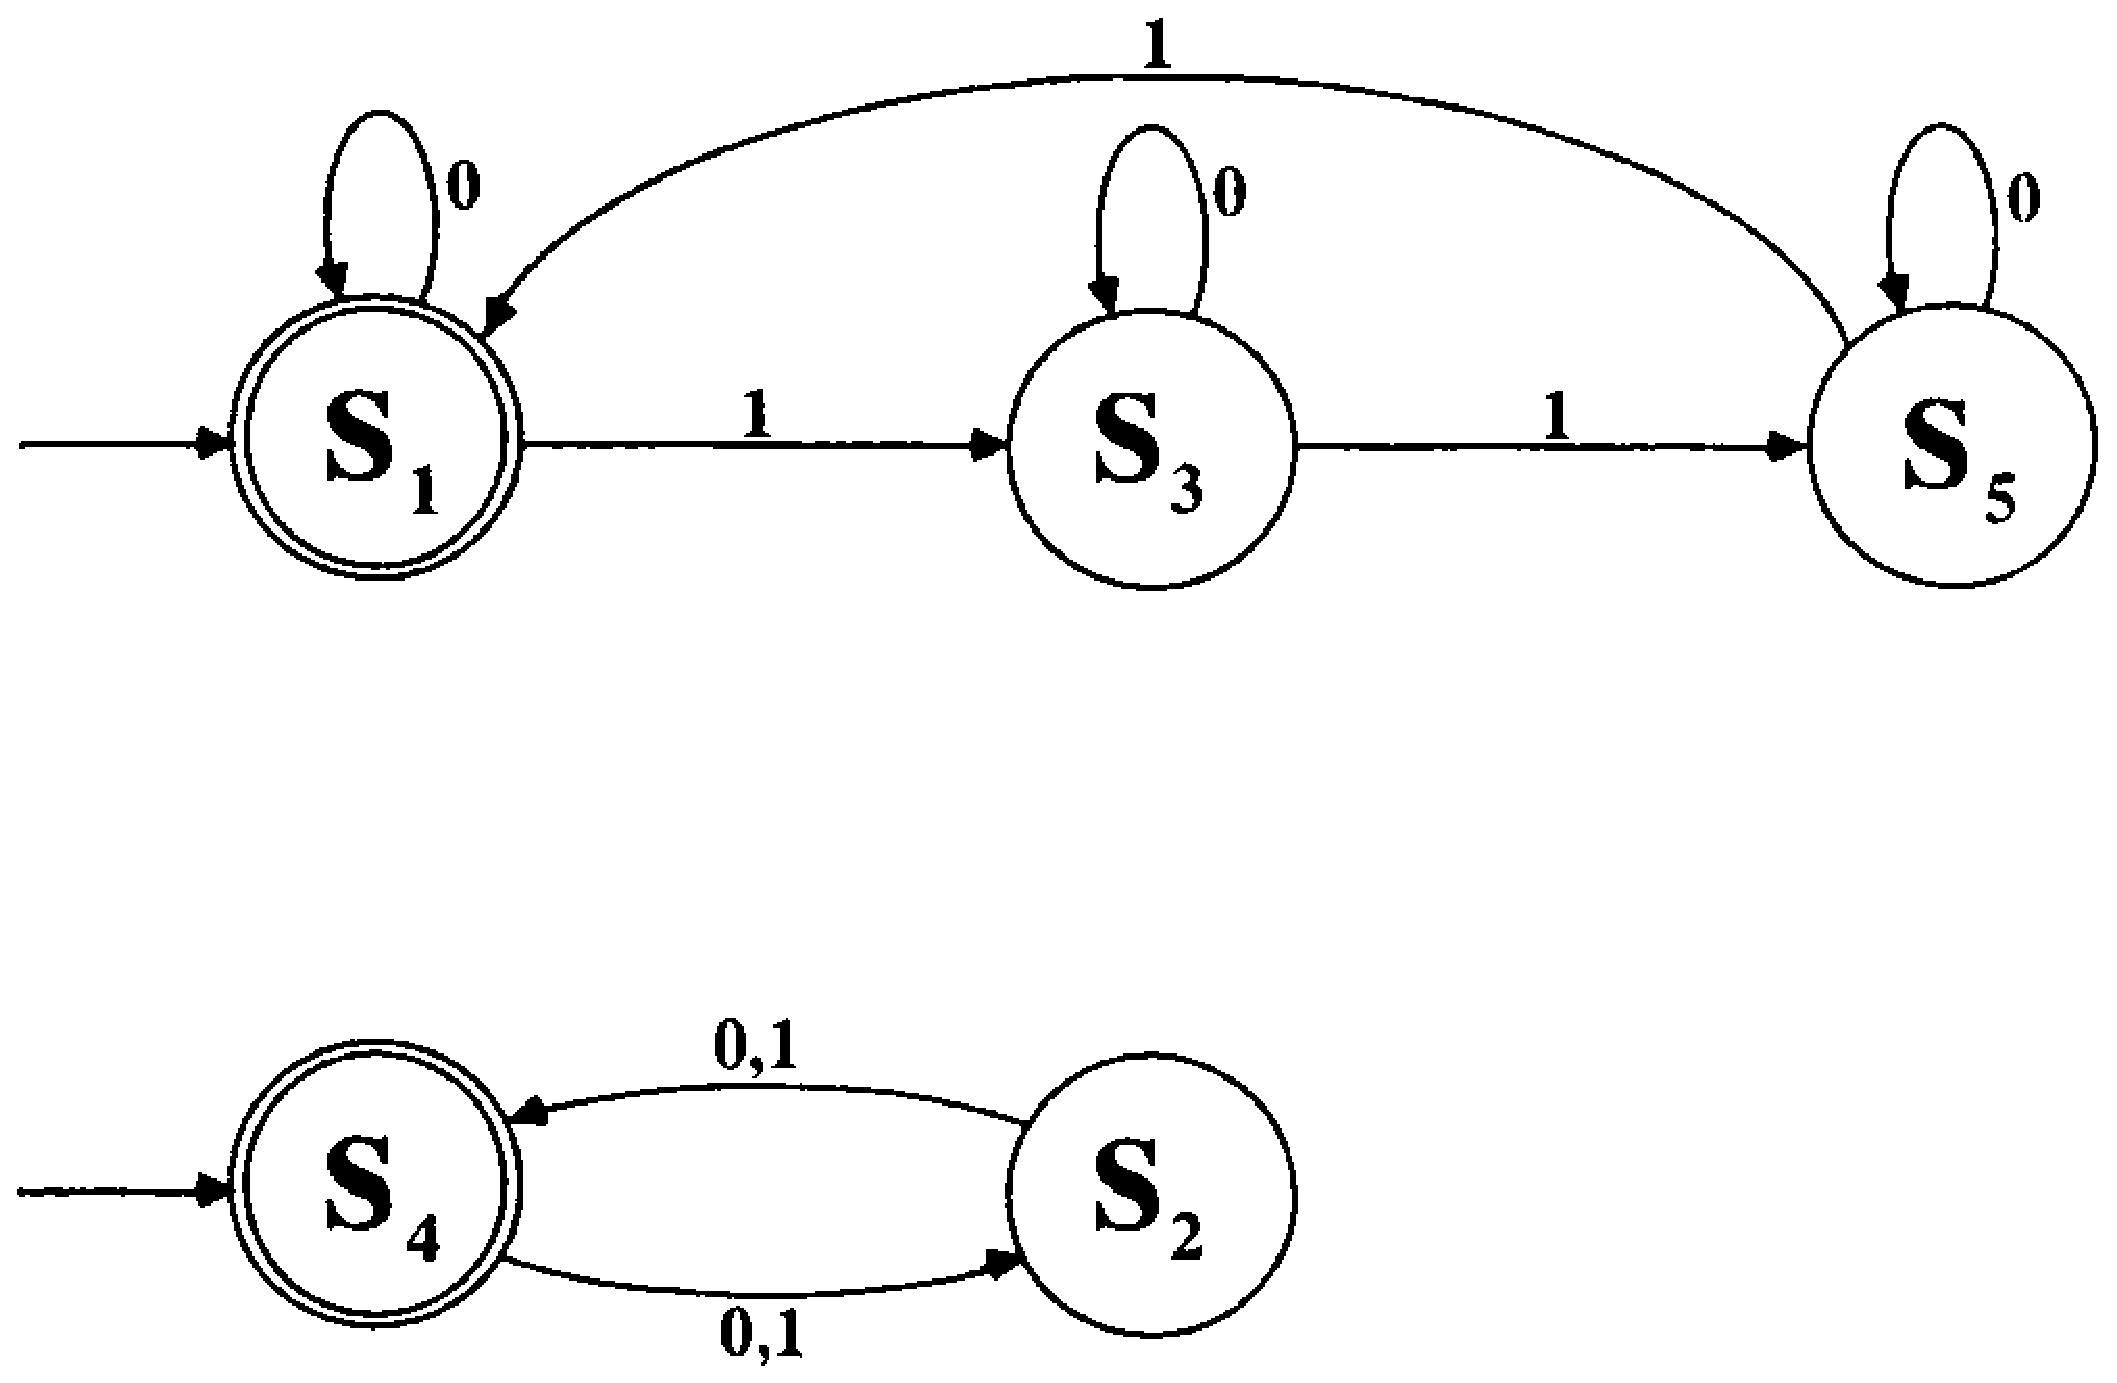
\epsfig{figure=ToFAfigures/fig4-4.eps,width=3in}}
\caption{The NDFA discussed in Example 4.3}\label{fig-4.4}
\end{figure}

As before, the addition of multiple start states to our computational model
facilitates machine construction but adds no more recognition power. We turn
now to the formal definition of nondeterministic finite automata.

% Definition 4.1
\begin{dfn}\label{dfn-4.1}\index{final state!for NDFA}\index{state transition function!for NDFA}\index{finite automaton!nondeterministic}
A \emph{nondeterministic finite automaton}\index{nondeterministic finite automaton|see{NDFA}}(\Index{NDFA}) is a
quintuple $A=\langle\Sigma,S,S_0,\delta,F\rangle$ where:
\begin{enumerate}[i.]
\item $\Sigma$ is an alphabet.\index{alphabet!input}
\item $S$ is a finite nonempty set of states.
\item $S_0$ is a \emph{set} of initial states,\index{start state} a nonempty subset of $S$.
\item $\delta:\ S \times \Sigma \rightarrow \wp(S)$ is the state transition
function.
\item $F$ is the set of accepting states, a (possibly empty) subset of $S$.
\end{enumerate}
\end{dfn}

The input alphabet, the state space, and even the set of final states are the
same as for deterministic finite automata. The important differences are
contained in the definitions of the initial states and of the $\delta$ function.

The set of initial states can be any nonempty subset of the state space. These
can be viewed as multiple entry points into the machine, with each start state
beginning distinct, although not necessarily disjoint, paths through the machine.

The $\delta$ function for nondeterministic finite automata differs from the
$\delta$ function of deterministic machines in that it maps a single state and a
letter to a set of states. In some texts, one will find $\delta$ defined as
simply a relation with range $S$ and not as a function; without any loss of
generality we define $\delta$ as a function with range $\wp(S)$, which makes
the formal proofs of relevant theorems considerably easier.

\subsection*{Example 4.4}

Consider the machine $A=\langle\Sigma,S,S_0,\delta,F\rangle$, where
\begin{center}\begin{tabular}{rcl}
$\Sigma$ & $=$ & $\{\pmb{a},\pmb{b}\}$ \\
$S$ & $=$ & $\{r,s,t\}$ \\
$S_0$ & $=$ & $\{r,s\}$ \\
$F$ & $=$ & $\{t\}$
\end{tabular}\end{center}
and $\delta:\ \{r,s,t\} \times \{\pmb{a},\pmb{b}\} \rightarrow \{\emptyset,
\{r\},\{s\},\{t\},\{s,t\},\{r,s\},\{r,t\},\{r,s,t\}\}$ is given
in Figure \ref{fig-4.5}.
% Figure 4.5
\begin{figure}[h]
\begin{center}\begin{tabular}{c|cc}
$\delta$ & $\pmb{a}$ & $\pmb{b}$ \\
\hline
r & $\{s\}$ & $\emptyset$ \\
s & $\emptyset$ & $\{r,t\}$ \\
t & $\emptyset$ & $\{t\}$
\end{tabular}\end{center}
\centerline{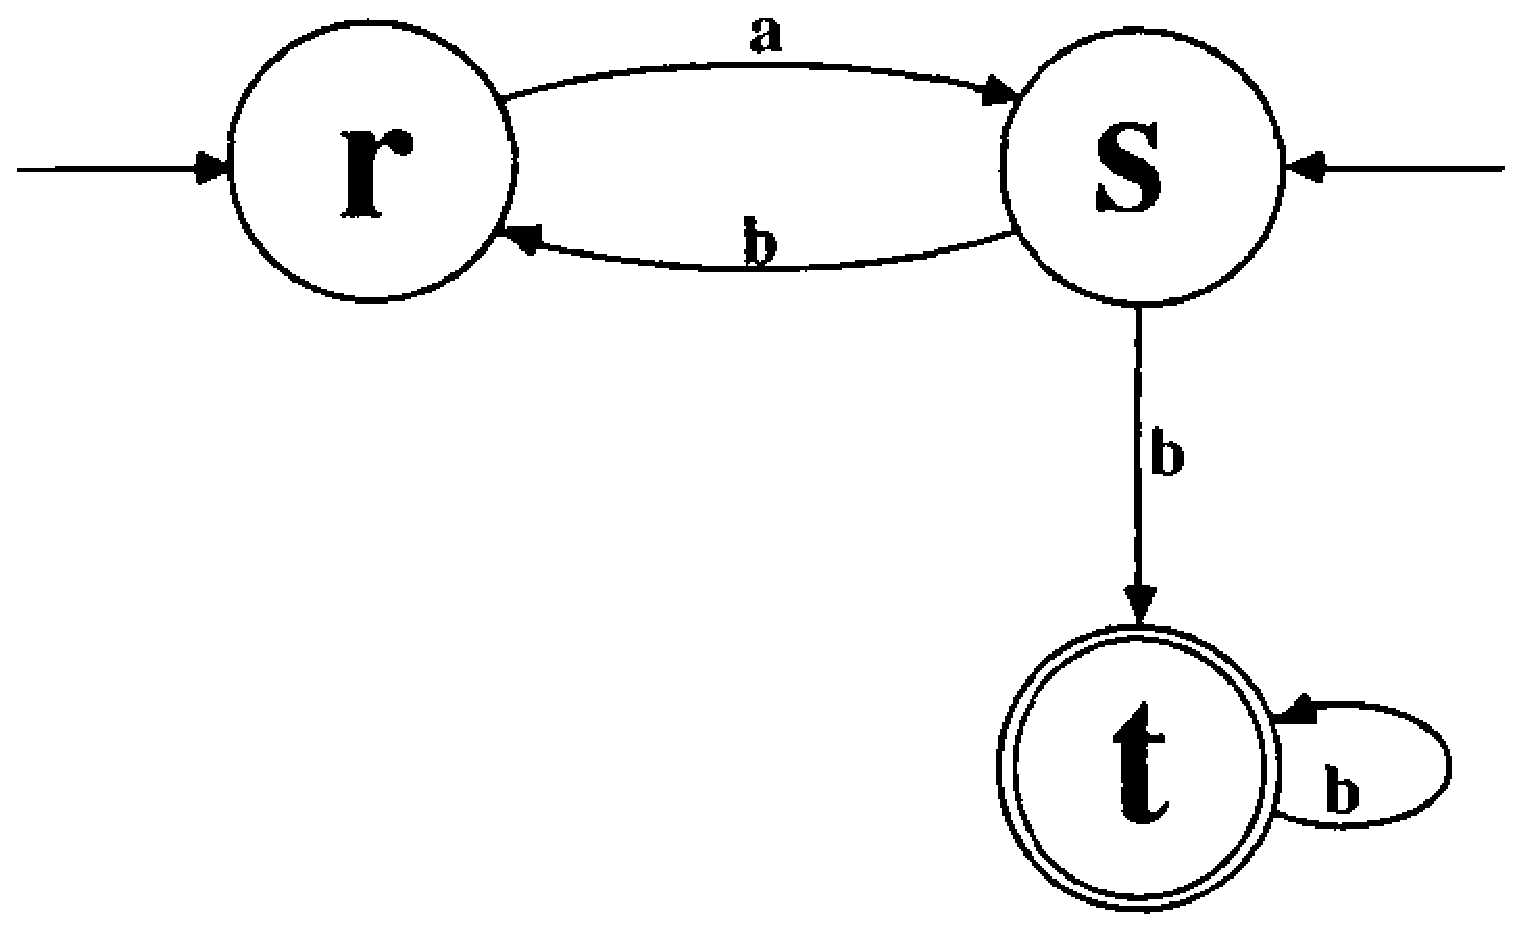
\epsfig{figure=ToFAfigures/fig4-5.eps,width=2.5in}}
\caption{An NDFA state transition diagram corresponding to the formal definition
given in Example 4.4}\label{fig-4.5}
\end{figure}

We will see later that this machine accepts strings that begin with alternating
$\pmb{a}$s and $\pmb{b}$s and end with one or more consecutive $\pmb{b}$s

% Definition 4.2
\begin{dfn}\label{dfn-4.2}\index{extended state transition function \DBAR\! for NDFA}
Given an NDFA $A=\langle\Sigma,S,S_0,\delta,F\rangle$, the
\emph{extended state transition function} for $A$ is the function $\DBAR:\ S
\times \Sigma^* \rightarrow \wp(S)$ defined recursively as follows: \\
\begin{center}\begin{tabular}{c}
$(\forall s \in S)\ \ \DBAR(s,\lambda) = \{s\}$ \\
$(\forall s \in S)(\forall\pmb{a}\in\Sigma)(\forall x \in \Sigma^*)\ \ 
	\DBAR(s,x\pmb{a}) = \bigcup\limits_{q\,\in\,\DBAR(s,x)}\delta(q,
	\pmb{a})$
\end{tabular}\end{center}
\end{dfn}

Once again, $\DBAR(s,x)$ is meant to represent where we arrive after starting at
a state $s$ and processing all the letters of the string $x$. In the case of
nondeterministic finite automata, $\DBAR$ does not map to a single state but to
a set of states because of the possible multiplicity of paths.

\subsection*{Example 4.5}

Consider again the NDFA displayed in Example 4.4. To find all the places a
string such as $\pmb{bb}$ can reach from $s$, we would first determine what can be
reached by the first $\pmb{b}$. The reachable states are $r$ and $t$, since
$\DBAR(s,\pmb{b}) = \{r, t\}$. From these states, we would then determine what
could be reached by the second $\pmb{b}$ (from $r$, no progress is possible, but
from $t$, we can again reach $t$). These calculations are reflected in the
recursive definition of $\DBAR$:
\[ \DBAR(s,\pmb{bb}) = \bigcup\limits_{q\,\in\,\DBAR(s,\pmb{b})}\delta
	(q,\pmb{b}) = \bigcup\limits_{q\,\in\,\{r,t\}}\delta(q,\pmb{b}) =
	\delta(r,\pmb{b}) \cup \delta(t,\pmb{b}) = \{\ \} \cup \{t\} = \{t\} \]

Because of the multiplicity of initial states and because the $\delta$ function
is now set-valued, it is possible for a nondeterministic finite automaton to be
active in more than a single state at one time. Whereas in all deterministic
finite automata there is a unique path through the machine labeled with
components of $w$ for each $w \in \Sigma^*$, this is not necessarily the case
for nondeterministic finite automata. At any point in the processing of a
string, the $\delta$ function maps the input symbol and the current state to a
set of states. This implies that multiple paths through the machine are possible
or that the machine can get ``stuck'' and be unable to process the remainder of
the string if there is no transition from a state labeled with the appropriate
letter. There is no more than one path for each word if there is exactly one
start state and the $\delta$ function always maps to a singleton set (or
$\emptyset$). If we were to further require that the $\delta$ function have a
defined transition to another state for every input symbol, then the machine
that we have would essentially be a deterministic finite automaton. Thus, all
deterministic finite automata are simply a special class of nondeterministic
finite automata; with some trivial changes in notation, any DFA can be thought
of as an NDFA. Indeed, the state transition diagram of a DFA could be a picture
of a well-behaved NDFA. Therefore, any language accepted by a DFA can be
accepted by an NDFA.

\subsection*{Example 4.6}

Consider the machine given in Example 4.4 and let $x = \pmb{b}$; the possible
paths through the machine include (1) starting at $s$ and proceeding to $r$, and
(2) starting at $s$ and proceeding to $t$. Note that it is not possible to start
from $t$ (since $t \notin S_0$), and there is no way to proceed with $x =
\pmb{b}$ by starting at $r$, the other start state.

Now let $x = \pmb{ba}$ and consider the possibilities. The only path through the
machine requires that we start at $s$, proceed to $r$, and return to $s$;
starting at $s$ and proceeding to $t$ leaves no way to process the second letter
of $x$. Starting from $r$ is again hopeless (what types of strings are good
candidates for starting at $r$?).

Now let $x = \pmb{bab}$; the possible paths through the machine include (1)
starting at $s$, proceeding to $r$, returning to $s$, and then moving again to
$r$, and (2) starting at $s$, proceeding to $r$, returning to $s$, and then
proceeding to $t$. Note that starting at $s$ and moving immediately to $t$ again
leaves us with no way to process the remainder of the string. Both $\pmb{b}$ and
$\pmb{bab}$ included paths that terminated at the final state $t$ (among other
places). These strings will be said to be \emph{recognized} by this NDFA
(compare with Definition \ref{dfn-4.3}). $\pmb{ba}$ had no path that led to a final state,
and as a consequence we will consider $\pmb{ba}$ to be rejected by this machine.

There are a number of ways in which to conceptualize a nondeterministic
finite automaton. Among the most useful are the following two schemes:

\begin{enumerate}
\item At each state where a multiple transition occurs, the machine replicates
into identical copies of itself, with each copy following one of the possible
paths.
\item Multiple states of the machine are allowed to be active, and each of the
active states reacts to each input letter.
\end{enumerate}

It happens that the second viewpoint is the most useful for our purposes. From
a theoretical point of view, we use this as the basis for proving the
equivalence of deterministic and nondeterministic finite automata. It is also a
useful model upon which to base the circuits that implement NDFAs.

The concept of a language for nondeterministic finite automata is different
from that for deterministic machines. Recall that the requirement for a word
to be contained in the language accepted by a deterministic finite automaton was
that the processing of a string would terminate in a final state. This is also
the condition for belonging to the \emph{language} accepted by a
nondeterministic finite automaton; however, since the path through a
nondeterministic finite automaton is not necessarily unique, only one of the
many possible paths need terminate in a final state for the string to be
accepted.

% Definition 4.3
\begin{dfn}\label{dfn-4.3}
Let $A=\langle\Sigma,S,S_0,\delta,F\rangle$ be a nondeterministic finite
automaton and $w$ be a word in $\Sigma^*$. A accepts $w$ iff 
$(\bigcup\limits_{q\,\in S_0}\DBAR(q,w)) \cap F \not= \emptyset$.
\end{dfn}

Again conforming with our previous usage, a word that is not accepted is
\emph{rejected}. The use of the operator $L$ will be consistent with its usage in
previous chapters, although it does have a different formal definition. As
before, $L(A)$ is used to designate all those strings that are accepted by a
finite automaton $A$. Since the concept of \emph{acceptance} must be modified
for nondeterministic finite automata, the formal definition of $L$ is
necessarily different (contrast Definitions \ref{dfn-4.3} and \ref{dfn-1.12}).

% Definition 4.4
\begin{dfn}\label{dfn-4.4}
Given an NDFA $A=\langle\Sigma,S,S_0,\delta,F\rangle$, the language accepted
by $A$, denoted $L(A)$, is given by
\[L(A) = \{x \in \Sigma^*\,\,|\,\,(\bigcup\limits_{q\,\in S_0}
\DBAR(q,x)) \cap F \not= \emptyset\}\]
\end{dfn}

Occasionally, it will be more convenient to express $L(A)$ in the following
fashion: $L(A) = \{x \in \Sigma^*|\exists t \in S_0 \ni \DBAR(t,x) \cap F \not=
\emptyset\}$. The concept of \emph{equivalent} automata is unchanged: two
machines are equivalent \emph{iff} they accept the same language. Thus, if one
or both of the machines happen to be nondeterministic, the definition still
applies. For example, the NDFAs given in Figures \ref{fig-4.3} and \ref{fig-4.4} are equivalent.

The language recognized by a nondeterministic finite automaton is the set of
all words where at least one of the paths through the machine labeled with
components of that word ends in a final state. In other words, the set of
terminal states at the ends of the paths labeled by components of a word $w$
must have a state in common with the set of final states in order for $w$ to
belong to $L(A)$.

As a first example, refer to the NDFA defined in Example 4.4. As illustrated
in Example 4.6, this machine accepts strings that begin with alternating
$\pmb{a}$s and $\pmb{b}$s and end with one or more consecutive $\pmb{b}$s.

\subsection*{Example 4.7}

For a more concrete example, consider the problem of a ship attempting to
transmit data to shore at random intervals. The receiver must continually
listen, usually to noise, and recognize when an actual transmission starts so
that it can record the data that follow. Let us assume that the start of a
transmission is signaled by the string $\pmb{010010}$ (in practice, such a
signal string should be much longer to minimize the possibility of random noise
triggering the recording mechanism). In essence, we wish to build an NDFA that
will monitor a bit stream and move to a final state when the substring
$\pmb{010010}$ is detected (note that nonfinal states correspond to having the
recording mechanism off, and final states signify that the current data should
be recorded). The reader is encouraged to discover firsthand how hard it is to
build a DFA that correctly implements this machine and contrast that solution to
the NDFA $T$ given in Figure \ref{fig-4.6}.

% Figure 4.6
\begin{figure}
\centerline{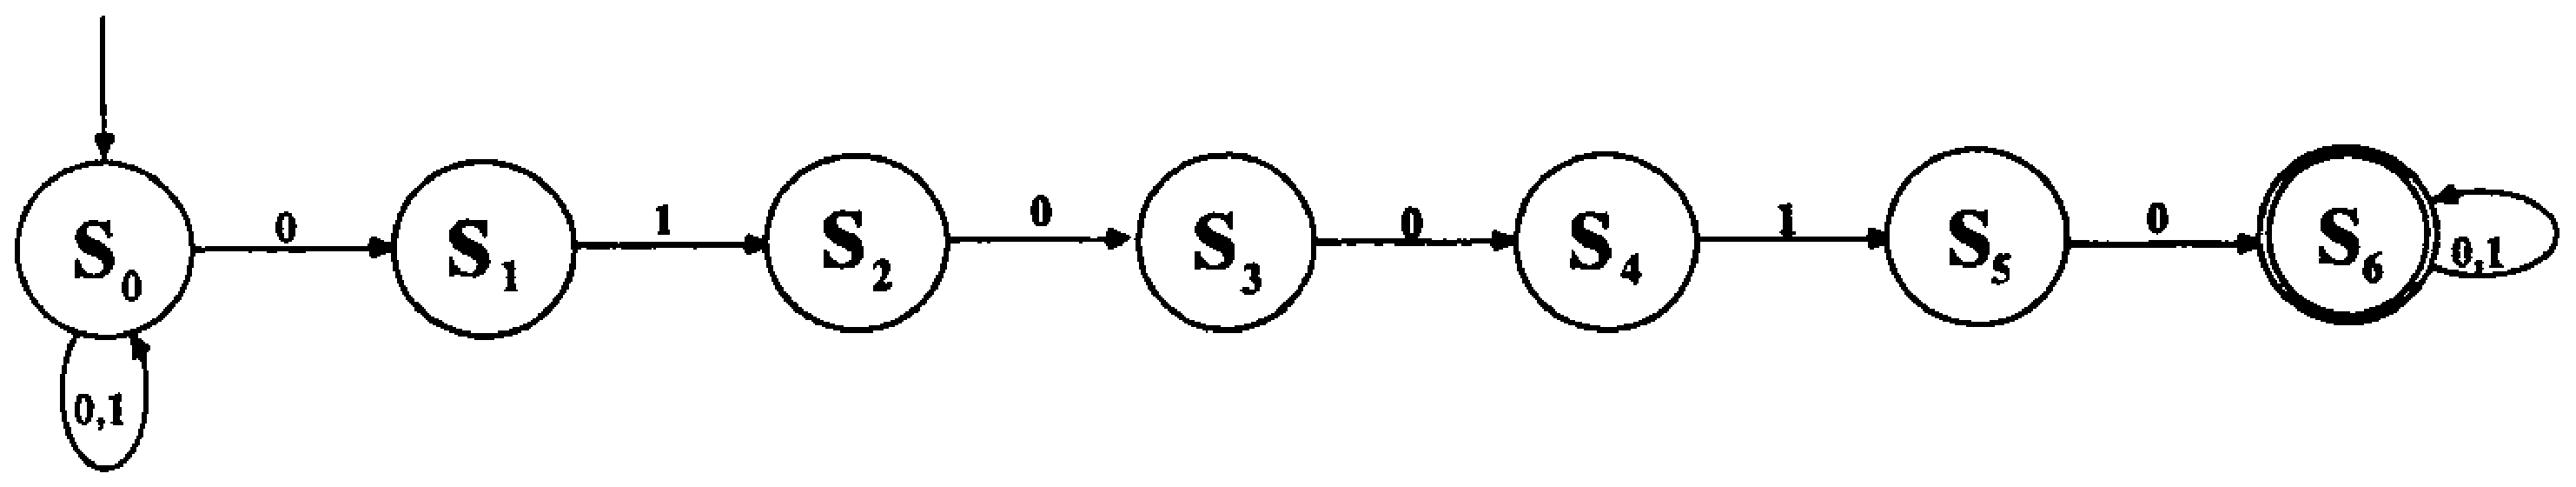
\epsfig{figure=ToFAfigures/fig4-6.eps,width=6.5in}}
\caption{An NDFA for pattern recognition}\label{fig-4.6}
\end{figure}

Since the transitions leading to higher states are labeled by the symbols in
$\pmb{010010}$, it is clear that the last state cannot be reached unless the
sequence $\pmb{010010}$ is actually scanned at some point during the processing
of the input string. Thus, the NDFA clearly accepts no word that should be
rejected. Conversely, since \emph{all} possible legal paths are explored by an
NDFA, valid strings \emph{will} find a way to the final state. lt is sometimes
helpful to think of the NDFA as remaining in $s_0$ while the initial part of the
input string is being processed and then ``guessing'' when it is the right time
to move to $s_1$.

It is also possible to model an end-of-transmission signal that turns the
recording device off (see the exercises). The device would remain in various
final states until a valid end-of-transmission string was scanned, at which
point it would return to the (nonfinal) start state.

While the NDFA given in Example 4.6 is very straightforward, it appears to be
hard to simulate this nondeterminism in real time with a deterministic computer.
It has not been difficult to keep track of the multiple paths in the simple
machines seen so far. However, if each state has multiple transitions for a
given symbol, the number of distinct paths a single word can take through an
NDFA grows exponentially as the length of the word increases. For example, if
each transition allowed a choice of three destination states, a word of length
$m$ would have $3^m$ possible paths from one single start state. An improvement
can be made by calculating, as each letter is processed, the set of possible
\emph{destinations} (rather than recording all the \emph{paths}). Still, in an
$n$-state NDFA, there are potentially $2^n$ such combinations of states. This
represents an improvement over the path set, since now the number of state
combinations is independent of the length of the particular word being
processed; it depends only on the number of states in the NDFA, which is
fixed. We will see that keeping track of the set of possible destination states
is indeed the best way to handle an NDFA in a deterministic manner.

Since we have seen in Chapter \ref{ch-1} that it is easy to implement a DFA, we now
explore methods to convert an NDFA to an equivalent DFA. Suppose that we are
given a nondeterministic finite automaton $A$ and that we want to construct a
corresponding deterministic finite automaton $A^d$. Using the concepts in
Definitions \ref{dfn-4.1} through \ref{dfn-4.4}, we can proceed in the following fashion. Our
general strategy will be to keep track of all the states that can be reached by
some string in the nondeterministic finite automaton. Since we can arbitrarily
label the states of an automaton, we let the state space of $A^d$ be the
\emph{power set} of $S$. Thus, $S^d = \wp(S)$, and each state in the new
machine will be labeled by some subset of $S$. Furthermore, let the start state
of $A^d$, denoted $s^d_0$, be labeled by the member of $\wp(S)$ containing
those states that are initial states in $A$; that is, $s^d_0 = S_0$.

Since our general strategy is to ``remember'' all the states that can be reached
for some string, we can define the $\delta$ function in the following natural
manner: For every letter in $\Sigma$, let the new state transition function,
$\delta^d$, map to the subset of $\wp(S)$ labeled by the union of all those
states that are reached from some state contained in the current state name
(according to the old nondeterministic state transition function $\delta$).

According to Definition \ref{dfn-4.4}, for a word to be contained in the language accepted
by some nondeterministic finite automaton, at least one of the terminal states
was required to be contained in the set of final states. Thus, let the set of
final states in the corresponding deterministic finite automaton be labeled by
the subsets of $S$ that contain at least one of the accepting states in the
nondeterministic counterpart. The formal definition of our corresponding
deterministic finite automaton is given in Definition \ref{dfn-4.5}.

% Definition 4.5
\begin{dfn}\label{dfn-4.5}
Given an NDFA $A=\langle\Sigma,S,S_0,\delta,F\rangle$, the
\emph{\Index{corresponding deterministic finite automaton}}, $A^d=\langle\Sigma,
S^d,s^d_0,\delta^d,F^d\rangle$, is defined as follows:
\begin{center}\begin{tabular}{c}
$S^d = \wp(S)$ \\
$s^d_0 = S_0$ \\
$F^d = \{Q \in S^d|Q \cap F \not= \emptyset\}$
\end{tabular}\end{center}
and $\delta^d$ is the state transition function, $\delta^d$$:\ S^d \times \Sigma
\rightarrow S^d$, defined by
\[ (\forall Q \in S^d)(\forall\pmb{a}\in\Sigma)\delta^d(Q,\pmb{a}) =
	\bigcup\limits_{q\,\in\, Q} \delta(q,\pmb{a}) \]
$\delta^d$ extends to the function $\deltabar{d}\!\!:\ S^d \times \Sigma^* \rightarrow
S^d$ as suggested by Theorem \ref{thm-1.1}:
\begin{center}\begin{tabular}{l}
$(\forall Q \in S^d)\qquad\qquad\qquad\qquad\ \deltabar{d}(Q,\lambda) = Q$ \\
$(\forall Q \in S^d)(\forall\pmb{a}\in\Sigma)(\forall x \in
	\Sigma^*)\deltabar{d}(Q,x\pmb{a}) = \delta^d(\deltabar{d}(Q,x),\pmb{a})$
\end{tabular}\end{center}
\end{dfn}

Definition \ref{dfn-4.5} describes a deterministic finite automaton that observes the
same restrictions as all other deterministic finite automata (a single start
state, a finite state set, a well-defined transition function, and so on). The
only peculiarity is the labeling of the states. Note that the definition implies
that the state labeled by the empty set is \emph{never} a final state and that
all transitions from this state lead back to itself. This is the dead state,
which is reached by strings that are always prematurely terminated in the
corresponding nondeterministic machine.

\subsection*{Example 4.8}

Consider the NDFA $B$ given in Figure \ref{fig-4.7}. As specified by Definition \ref{dfn-4.5}, the
corresponding DFA $B^d$ would look like the machine shown in Figure \ref{fig-4.8}. Note
that all the states happen to be accessible in this particular example.

% Figure 4.7
\begin{figure}
\centerline{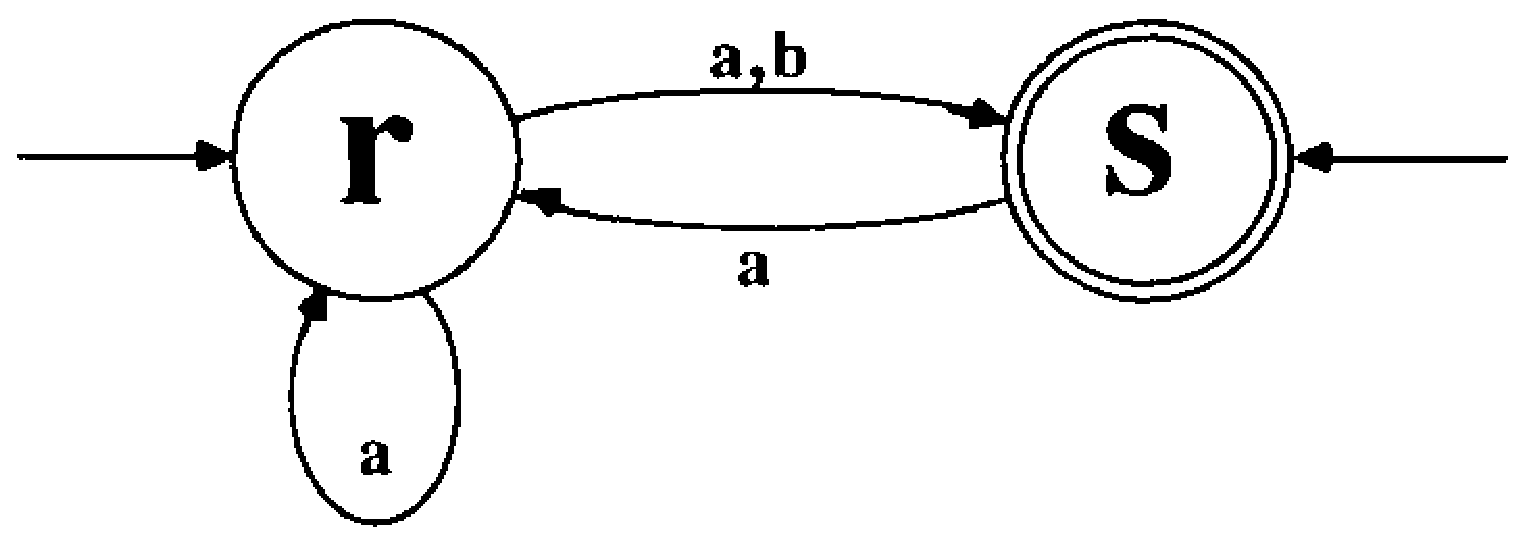
\epsfig{figure=ToFAfigures/fig4-7.eps,width=2.8in}}
\caption{The NDFA B discussed in Example 4.8}\label{fig-4.7}
\end{figure}

Since the construction of the corresponding deterministic machine involves
$\wp(S)$, it should be obvious to the reader that the size of this
deterministic finite automaton \emph{can} grow exponentially larger as the number of
states in the associated nondeterministic finite automaton increases. In
general, however, there are often many inaccessible states. Thus, only the
states that are found to be reachable during the construction process need to be
included. The reader is encouraged to exploit this fact when constructing
corresponding deterministic finite automata. The language accepted by the DFA
$A^d$ follows the definition given in Chapter \ref{ch-1}.

% Figure 4.8
\begin{figure}
\centerline{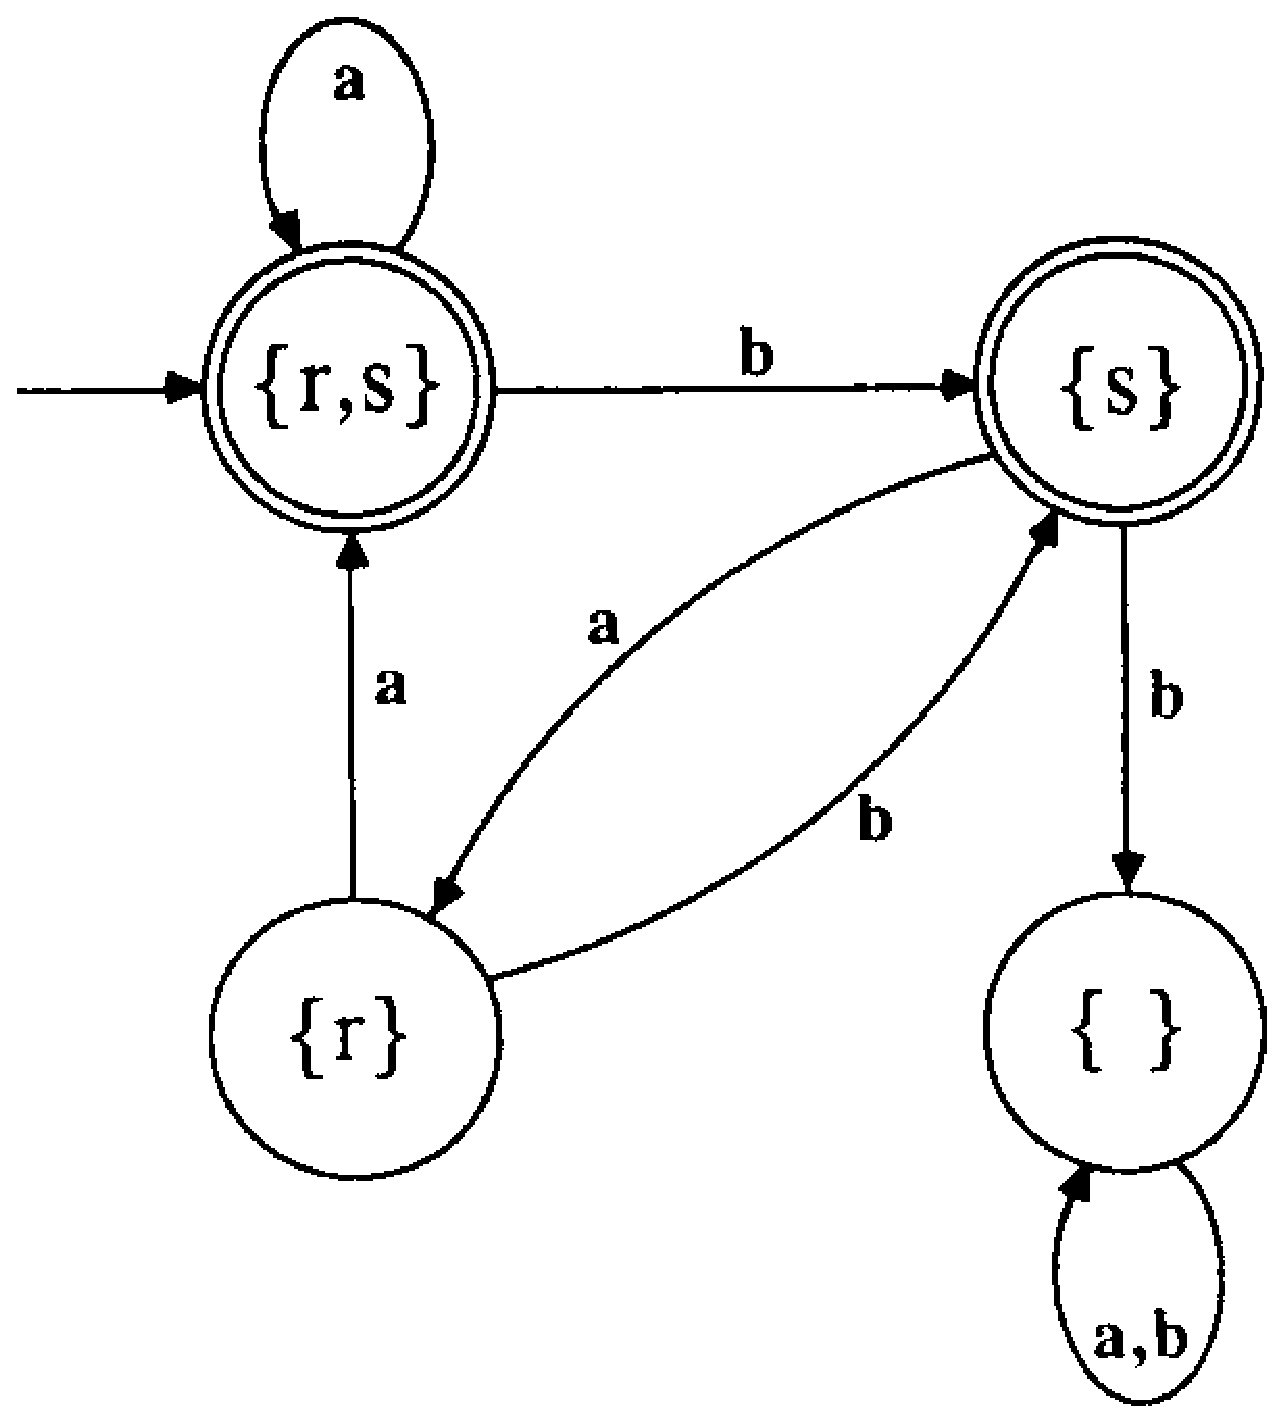
\epsfig{figure=ToFAfigures/fig4-8.eps,width=2.5in}}
\caption{The deterministic equivalent of the NDFA given in Example 4.8}\label{fig-4.8}
\end{figure}

To show that the deterministic finite automaton that we have just defined
accepts the same language as the corresponding nondeterministic finite
automaton, we must first show that the $\deltabar{d}$ function behaves in the same
manner for strings as the $\delta^d$ function does for single letters. For any
state $Q \in S^d$, the $\delta^d$ function maps this state and an input letter
$\pmb{a} \in \Sigma$ according to the mapping of the $\delta$ function for each
$q \in Q$ and the letter $\pmb{a}$. The following lemma establishes that $\deltabar{d}$
performs the corresponding mapping for strings.

% Lemma 4.1
\begin{lmm}\label{lmm-4.1}
Let $A=\langle\Sigma,S,S_0,\delta,F\rangle$ be a nondeterministic finite
automaton, and let $A^d=\langle\Sigma,S^d,s^d_0,\delta^d,F^d\rangle$ represent
the corresponding deterministic finite automaton. Then
\[ (\forall Q \in S^d)(\forall x \in \Sigma^*)(\deltabar{d}(Q,x) =
	\bigcup\limits_{q\,\in\, Q} \DBAR(q,x)) \]

\emph{Proof.} By induction on $|x|$: Let $P(k)$ be defined by
\[ P(k):\ (\forall Q \in S^d)(\forall x \in \Sigma^k)(\deltabar{d}(Q,x) =
	\bigcup\limits_{q\,\in\, Q} \DBAR(q,x)) \]
\emph{Basis step:} $|x| = 0 \Rightarrow x = \lambda$ and therefore
\[ \deltabar{d}(Q,\lambda) = Q = \bigcup\limits_{q\,\in\, Q}\{q\} = 
	\bigcup\limits_{q\,\in\, Q}\DBAR(q,\lambda) \]
\emph{Inductive step:} Suppose that the result holds for all $x \ni |x| = k$;
that is, $P(k)$ is true. Let $y \in \Sigma^{k+1}$. Then $\exists x \in \Sigma^k$
and $\exists \pmb{a} \in \Sigma \ni y = x\pmb{a}$. Then
\begin{center}\begin{tabular}{rcl}
$\deltabar{d}(Q,y)$ & $=$ & (by definition of $y$) \\
$\deltabar{d}(Q,x\pmb{a})$ & $=$ & (by Theorem \ref{thm-1.1}) \\
$\delta^d(\deltabar{d}(Q,x),\pmb{a})$ & $=$ & (by the induction hypothesis) \\
$\delta^d(\bigcup\limits_{q\,\in\, Q}\DBAR(q,x),\pmb{a})$ & $=$ & $(\forall A,B
	\in \wp(S))(\forall\pmb{a}\in\Sigma)(\delta^d(A \cup B,\pmb{a}) =
	\delta^d(A,\pmb{a}) \cup \delta^d(B,\pmb{a}))$ \\
$\bigcup\limits_{q\,\in\, Q}\delta^d(\DBAR(q,x),\pmb{a})$ & $=$ &
	(by Definition \ref{dfn-4.5}) \\
$\bigcup\limits_{q\,\in\, Q}(\bigcup\limits_{p\,\in\,\DBAR(q,x)}\delta
	(p,\pmb{a}))$ & $=$ & (by Definition \ref{dfn-4.2}) \\
$\bigcup\limits_{q\,\in\, Q}\DBAR(q,x\pmb{a})$ & $=$ & (by definition of $y$) \\
$\bigcup\limits_{q\,\in\, Q} \DBAR(q,y)$ &&
\end{tabular}\end{center}
Therefore, $P(k) \Rightarrow P(k+1)$ for all $k \geq 0$, and thus by the
principle of mathematical induction we can say that the result holds for all
$x \in \Sigma^*$.
\end{lmm}

Having established Lemma \ref{lmm-4.1}, proving that the language accepted by a
nondeterministic finite automaton and the corresponding deterministic machine
are the same language becomes a straightforward task. The equivalence of $A$ and
$A^d$ is given in the following theorem.

% Theorem 4.1
\begin{thm}\label{thm-4.1}
Let $A=\langle\Sigma,S,S_0,\delta,F\rangle$ be a nondeterministic finite
automaton, and let $A^d=\langle\Sigma,S^d,s^d_0,\delta^d,F^d\rangle$ represent
its corresponding deterministic finite automaton. Then $A$ and $A^d$ are
equivalent; that is, $L(A) = L(A^d)$.

\emph{Proof.} Let $x \in \Sigma^*$. Then
\begin{center}\begin{tabular}{rcl}
$x \in L(A)$ & $\Leftrightarrow$ & (by Definition \ref{dfn-4.4}) \\
$(\bigcup\limits_{s \in S_0}\DBAR(s,x)) \cap F \not= \emptyset$ &
	$\Leftrightarrow$ & (by Definition \ref{dfn-4.5}) \\
$(\bigcup\limits_{s\,\in\, S_0}\DBAR(s,x)) \in F^d$ & $\Leftrightarrow$ &
	(by Lemma \ref{lmm-4.1}) \\
$\DBAR^d(S_0,x) \in F^d$ & $\Leftrightarrow$ & (by Definition \ref{dfn-4.5}) \\
$\DBAR^d(s^d_0,x) \in F^d$ & $\Leftrightarrow$ & (by Definition \ref{dfn-1.15}) \\
$x \in L(A^d)$ &&
\end{tabular}\end{center}
\end{thm}

Now that we have established that nondeterministic finite automata and
deterministic finite automata are equal in computing power, the reader might
wonder why we bother with nondeterministic finite automata. Even though
nondeterministic finite automata cannot recognize any language that cannot be
defined by a DFA, they are very useful both in theory and in machine
construction (as illustrated by Example 4.7). The following examples further
illustrate that NDFAs often yield more natural (and less complex) solutions to a
given problem.

\subsection*{Example 4.9}

Recall the machine from Chapter \ref{ch-1} that accepted a subset of real constants in
scientific notation according to the following BNF:\index{BNF}\index{natural numbers}
\begin{center}
\begin{center}\begin{tabular}{rcl}
\hline
\<sign\> & ::= & $ \pmb + | \pmb -$ \\
\<digit\> & ::= & $ \pmb 0|\pmb 1|\pmb 2|\pmb 3|\pmb 4|\pmb 5|\pmb 6|\pmb 7|\pmb 8|\pmb 9$ \\
\<natural\> & ::= & \<\text{digit}\>$|$\<digit\>\<natural\> \\
\<integer\> & ::= & \<natural\>$|$\<sign\>\<natural\> \\
\<real constant\> & ::= & \<integer\> \ \ \ \ \ \ \ \ \ \ \ \ \ \ \ \ \ \ \ \ \ \ \ \ $|$ \\
 & &\ \ \<integer\>\pmb{.}  \ \ \ \ \ \ \ \ \ \ \ \ \ \ \ \ \ \ \ \ \ $|$ \\
 & &\ \ \<integer\>\pmb{.}\<natural\> \ \,$|$ \\
 & &\ \ \<integer\>\pmb{.}\<natural\>\pmb{E}\<integer\> \\
\hline
\end{tabular}\end{center}
\end{center}
By using nondeterministic finite automata, it is easy to construct a machine
that will recognize this language (compare with the deterministic version given
in Example 1.11). One such NDFA is shown in Figure \ref{fig-4.9}.


% Figure 4.9
\begin{figure}
\centerline{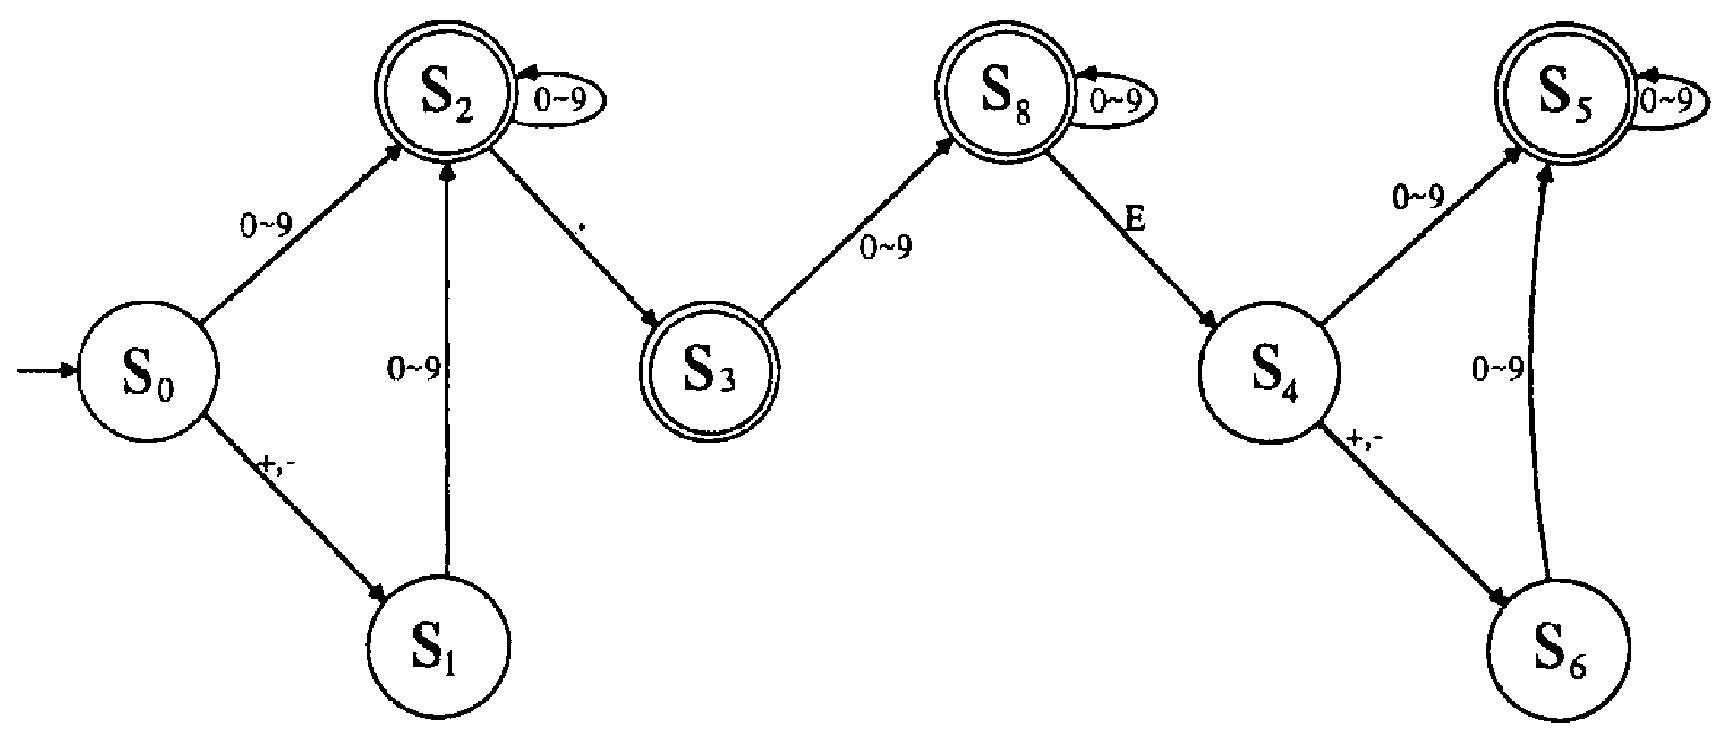
\epsfig{figure=ToFAfigures/fig4-9.eps,width=6in}}
\caption{The NDFA discussed in Example 4.9}\label{fig-4.9}
\end{figure}

\subsection*{Example 4.10}

Let $L=\{x \in \{\pmb{a},\pmb{b}\}^*|\ x$ begins with $\pmb{a}\vee x$ contains
$\pmb{ba}$ as a substring$\}$. We can easily build a machine that will accept
this language, as illustrated in Figure \ref{fig-4.10}. Now suppose we wanted to construct
a machine that would accept the \emph{reverse} of this language, that is, to accept
$L^r=\{x \in \{\pmb{a},\pmb{b}\}^*|\ x$ ends with $\pmb{a}\vee x$ contains
$\pmb{ab}\}$. The machine that will accept this language can be built using
nondeterministic finite automata by simply exchanging the initial states and the
final states and by reversing the arrows of the $\delta$ function. The automaton
(definitely an NDFA in this case!) arising in this fashion is shown in Figure
\ref{fig-4.11}.

% Figure 4.10
\begin{figure}
\centerline{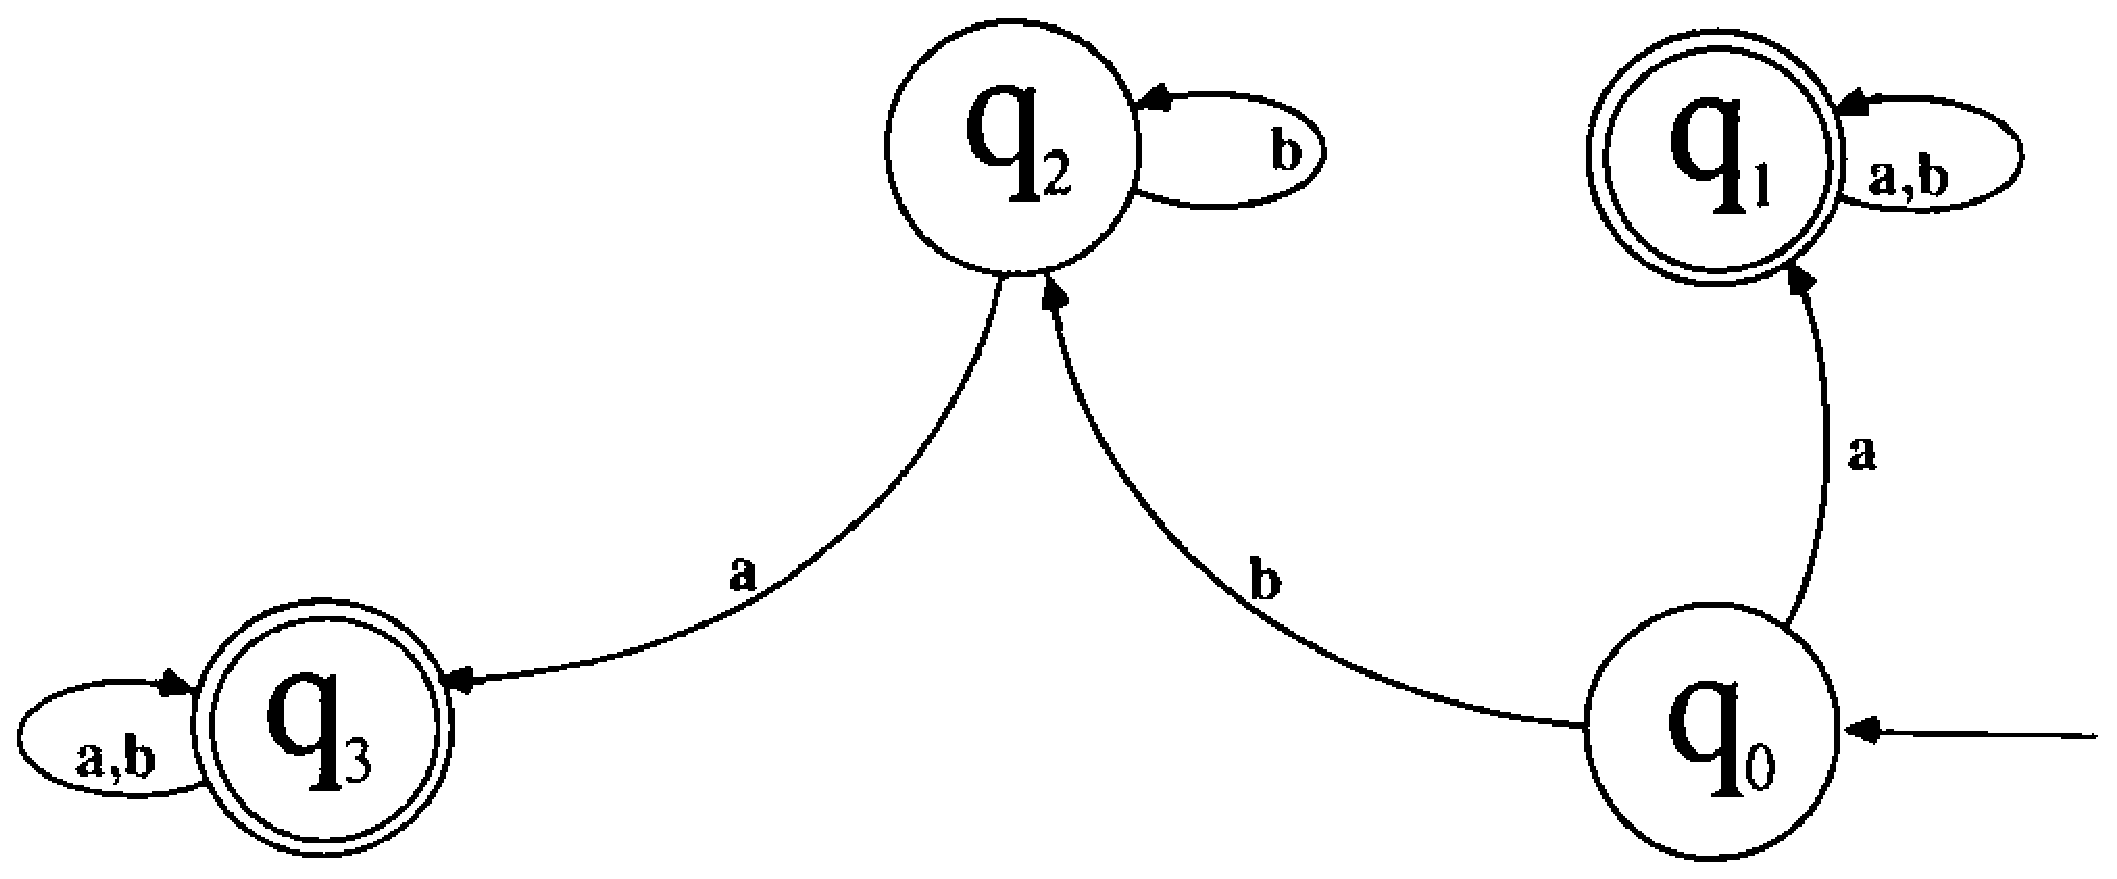
\epsfig{figure=ToFAfigures/fig4-10.eps,width=3.5in}}
\caption{An NDFA accepting the language given in Example 4.10}\label{fig-4.10}
\end{figure}

It can be shown that the technique employed in Example 4.10, when applied to \emph{any}
automaton, will yield a new NDFA that is guaranteed to accept the \emph{reverse}
of the original language. The material in Chapter \ref{ch-5} will reveal many instances
where the ability to define multiple start states and multiple transitions will
be of great value.

% Figure 4.11
\begin{figure}
\centerline{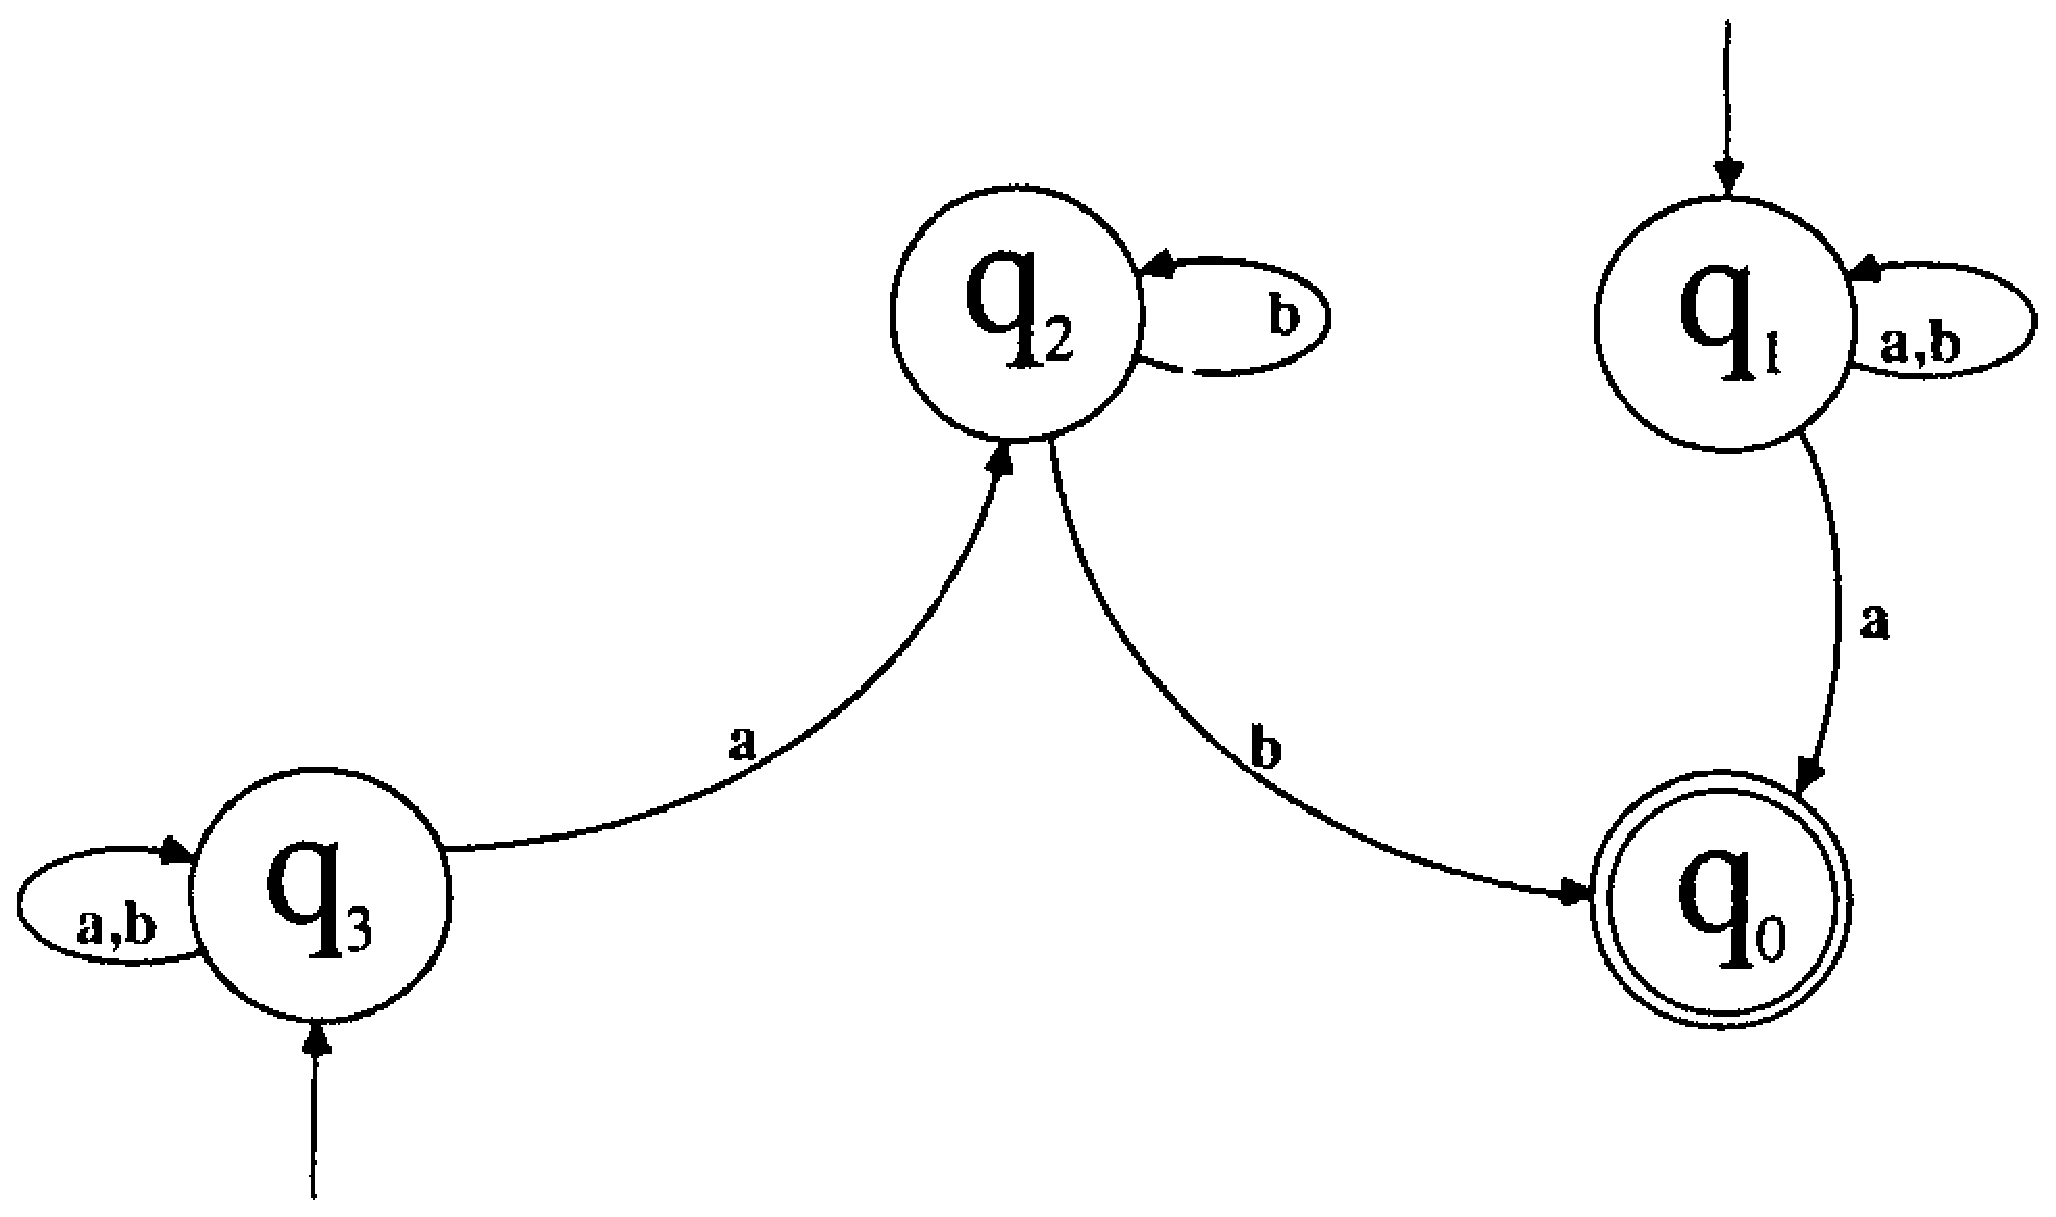
\epsfig{figure=ToFAfigures/fig4-11.eps,width=3.5in}}
\caption{An NDFA representing the reverse of the language represented in
Figure \ref{fig-4.10}}\label{fig-4.11}
\end{figure}

\subsection*{Example 4.11}

Assume we wish to identify all words that contain at least one of the three
strings $\pmb{10110},\ \pmb{1010}$, or $\pmb{01101}$ as substrings. Consequently, we let L be the set of all
words that are made up of some characters, followed by one of our three target
strings, followed by some other characters. That is,
\[ L=\{w \in \{\pmb{0},\pmb{1}\}^*|\ w=xyz,x \in \{\pmb{0},\pmb{1}\}^*,y \in
	\{\pmb{10110},\pmb{1010},\pmb{01101}\},z \in \{\pmb{0},\pmb{1}\}^*\} \]
We can construct a nondeterministic finite automaton that will accept this
language as follows. First construct three machines each of which will accept
one of the candidates for $y$. Next, prepend a single state ($s_0$ in Figure
\ref{fig-4.12}) that loops on $\Sigma^*$; make this state an initial state and draw arrows
from it which mimic the transitions from each of the other three initial states
(as shown in Figure \ref{fig-4.12}). Finally, append a single state machine ($S_{18}$)
that accepts $\Sigma^*$; draw arrows from each of the final states to this state. The machine that accepts this language is given in Figure \ref{fig-4.12}.
The reader is encouraged to try to construct a deterministic version of this
machine in order to appreciate the simplicity of the above solution.
(States $s_1$, $s_7$, and $s_{12}$ are shown for clarity,
but they are no longer needed.)

% Figure 4.12
\begin{figure}
\centerline{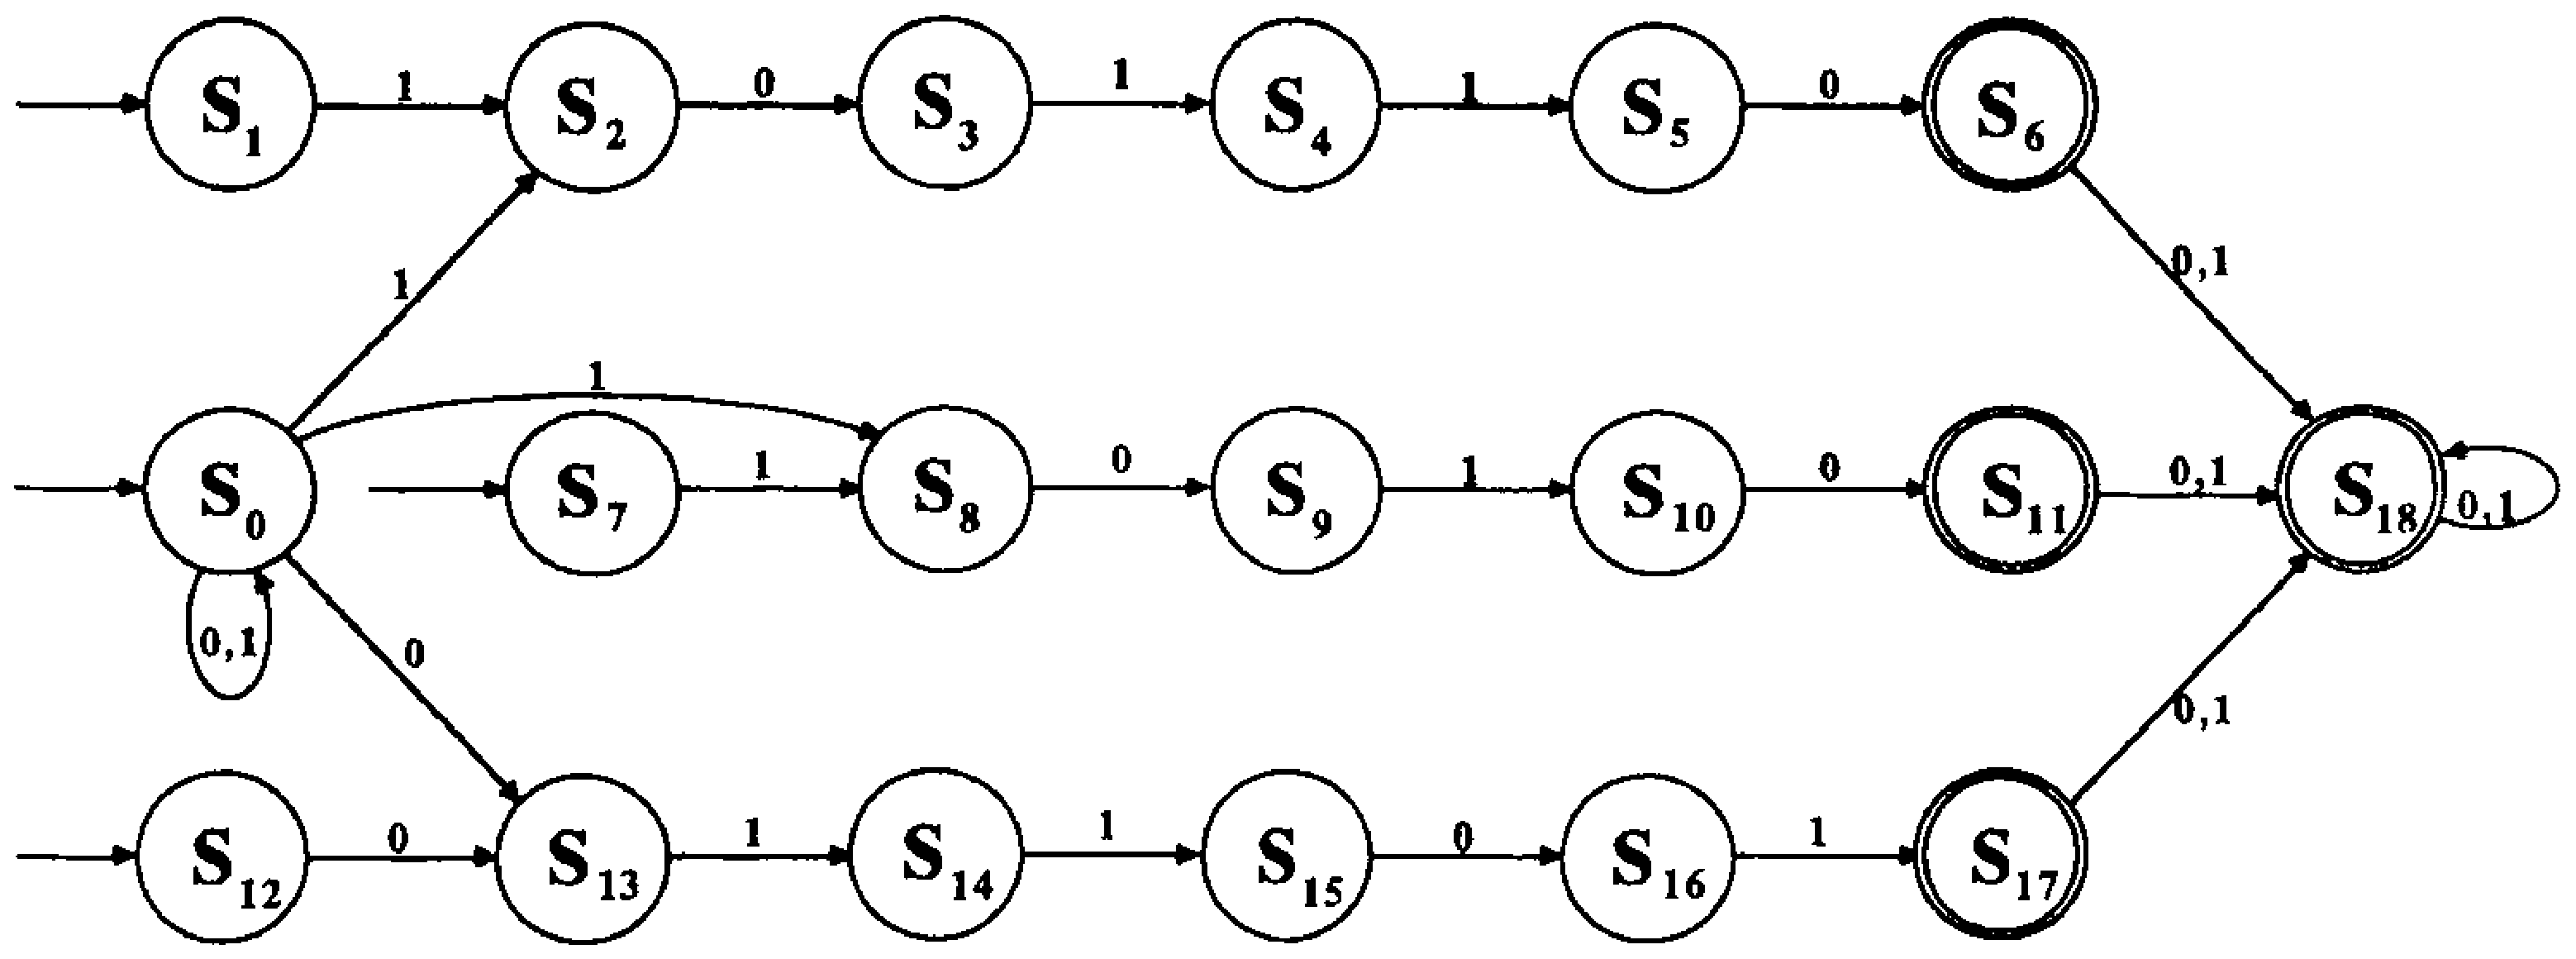
\epsfig{figure=ToFAfigures/fig4-12.eps,width=6.5in}}
\caption{An NDFA for recognizing any of several substrings}\label{fig-4.12}
\end{figure}

\subsection*{Example 4.12}

Recall the application in Chapter \ref{ch-1} involving string searching (Example
1.15). The construction of DFAs involved much thought, but there is an
NDFA that solves the problem in an obvious and straightforward manner. For
example, an automaton that recognizes all strings over the alphabet $\{\pmb{a},
\pmb{b}\}$ containing the substring $\pmb{aab}$ might look like the NDFA in
Figure \ref{fig-4.13}.

% Figure 4.13
\begin{figure}
\centerline{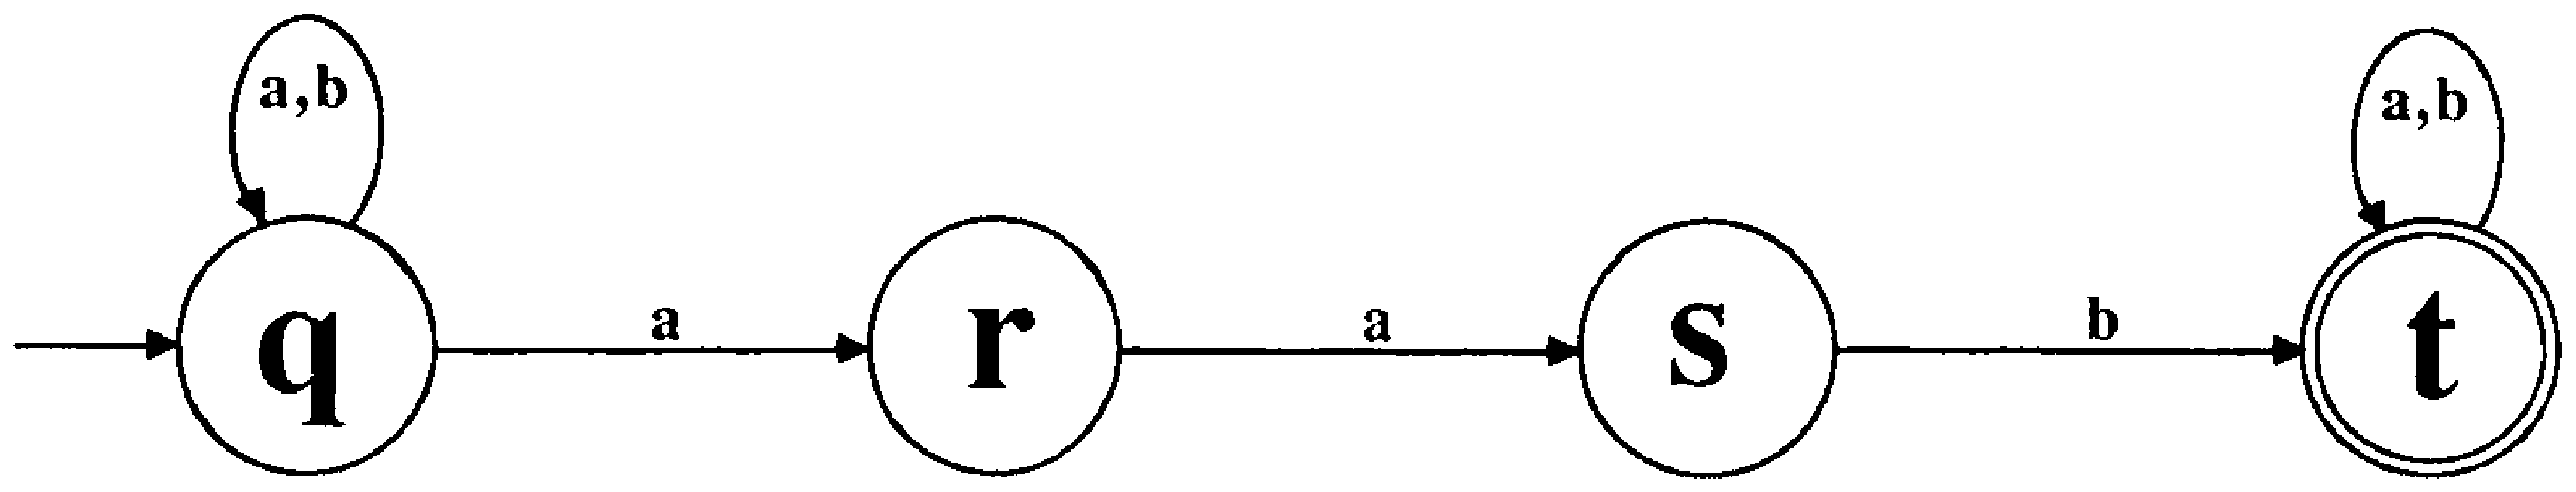
\epsfig{figure=ToFAfigures/fig4-13.eps,width=6.5in}}
\caption{An automaton recognizing the substring $\pmb{aab}$}\label{fig-4.13}
\end{figure}

As is the case for this NDFA, it may be impossible for certain sets of states
to all be active at once. These combinations can never be achieved during the
normal operation of the NDFA. The DFA states corresponding to these combinations
will not be in the connected part of $A^d$. Applying Definition \ref{dfn-4.5} to find the
entire deterministic version and then pruning it down to just the relevant
portion is very inefficient. A better solution is to begin at the start state
and ``follow transitions'' to new states until no further new states are
uncovered. At this point, the relevant states and their transitions will have
all been defined; the remainder of the machine can be safely ignored. For the
NDFA in Figure \ref{fig-4.13}, the connected portion of the equivalent DFA is shown in
Figure \ref{fig-4.14}. This automaton is still not reduced; the last three states are all
equivalent and can be coalesced to form the minimal machine given in Figure \ref{fig-4.15}.

% Figure 4.14
\begin{figure}
\centerline{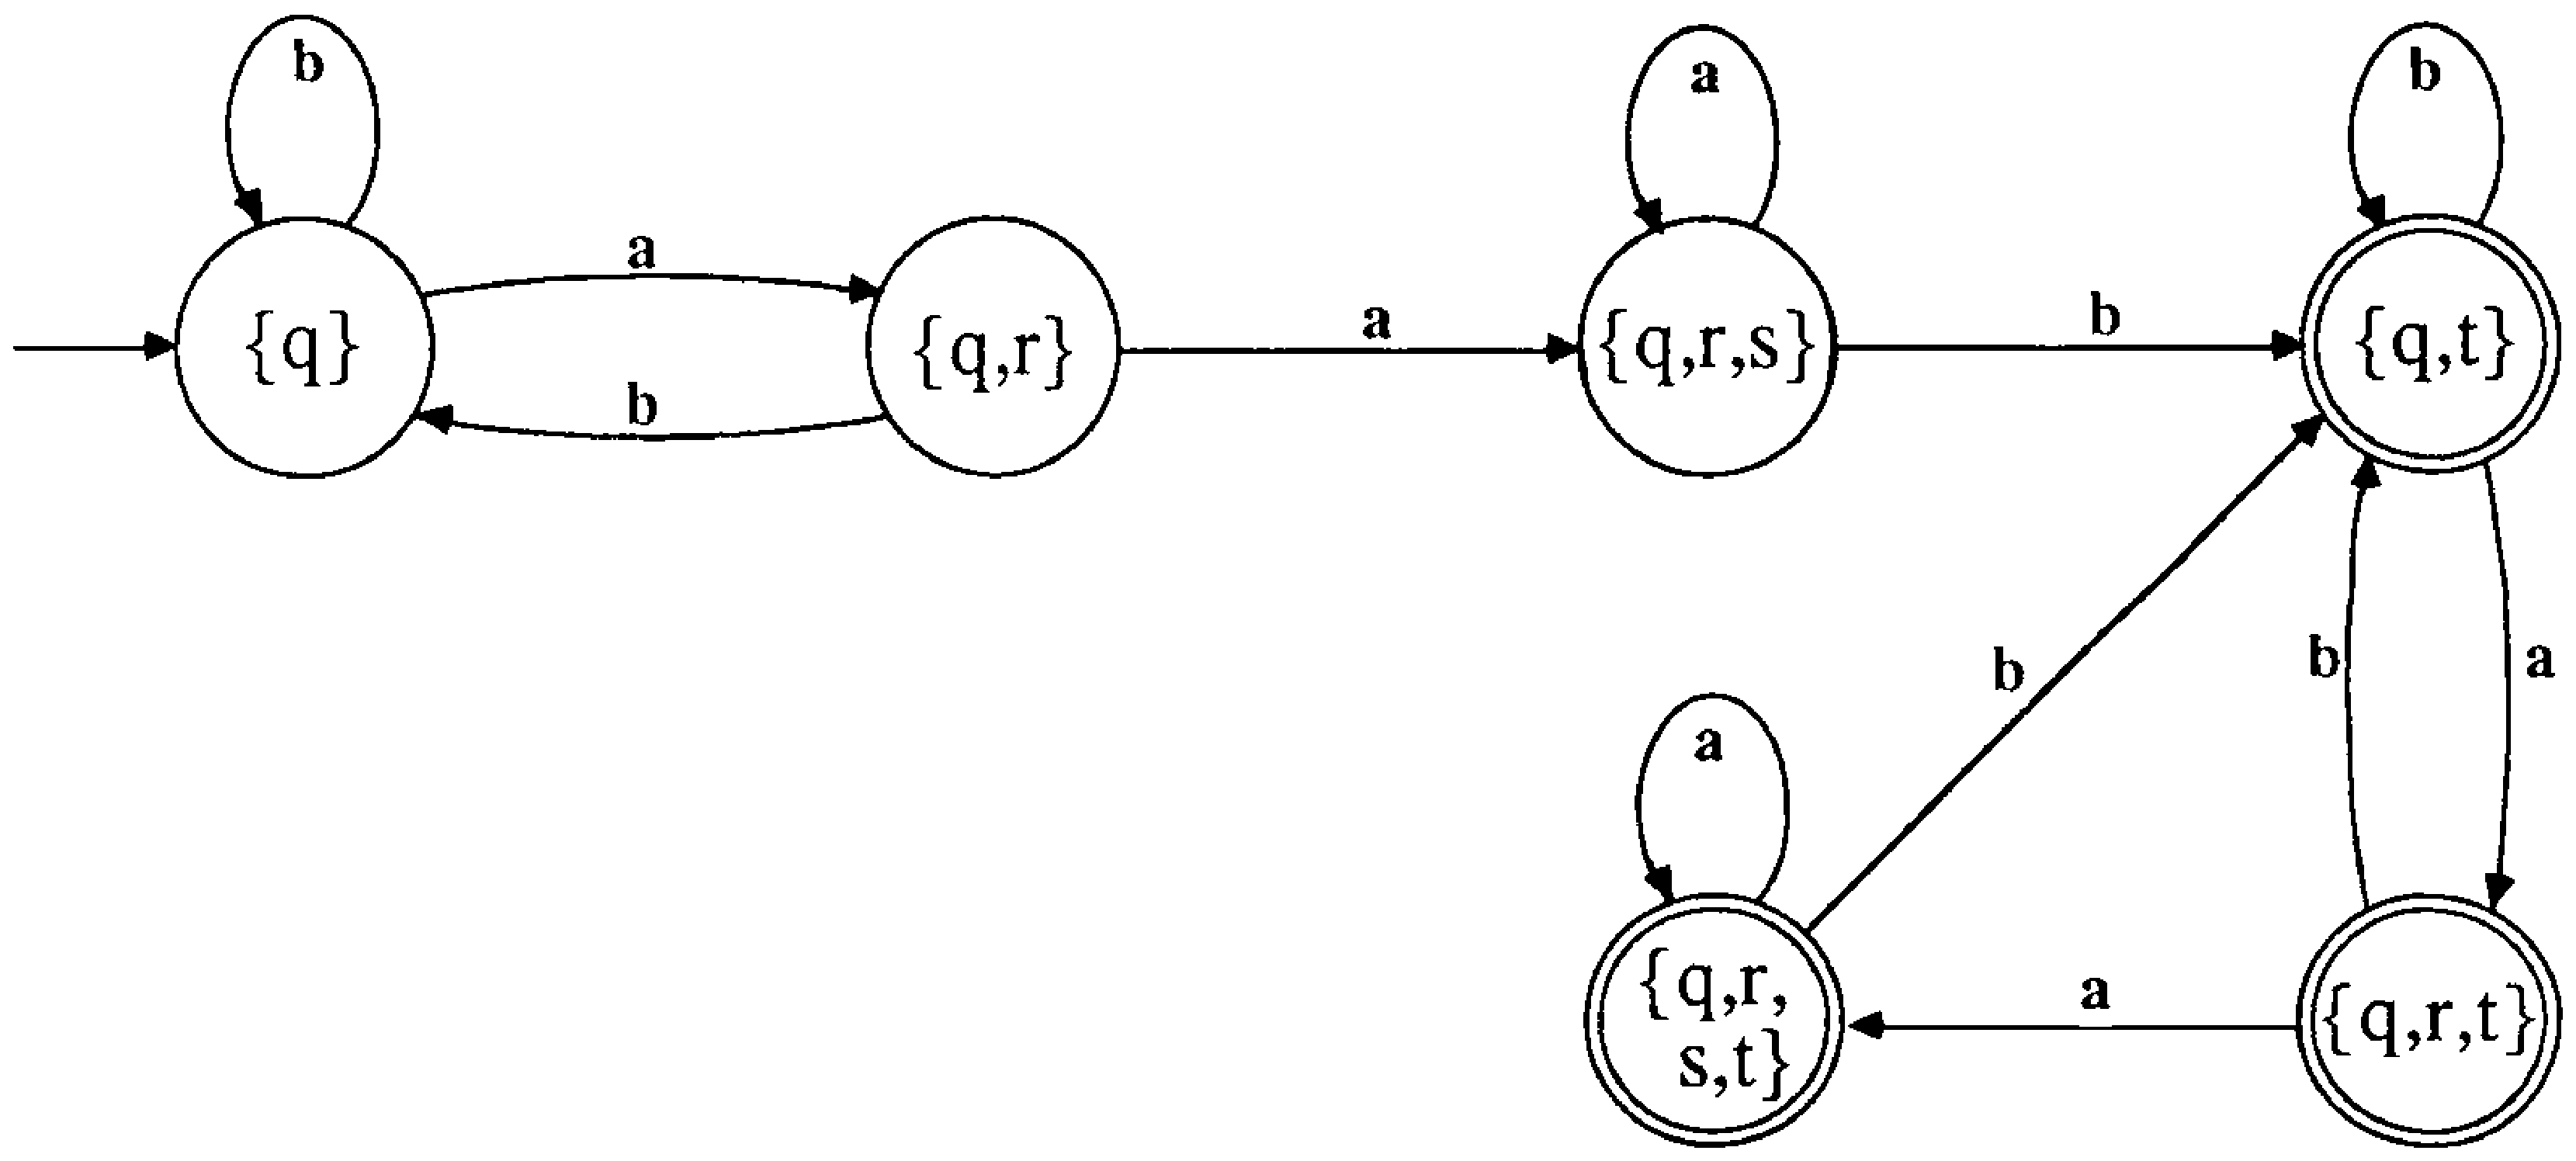
\epsfig{figure=ToFAfigures/fig4-14.eps,width=6.5in}}
\caption{The connected portion of the DFA equivalent to the NDFA given in
Example 4.12}\label{fig-4.14}
\end{figure}

% Figure 4.15
\begin{figure}
\centerline{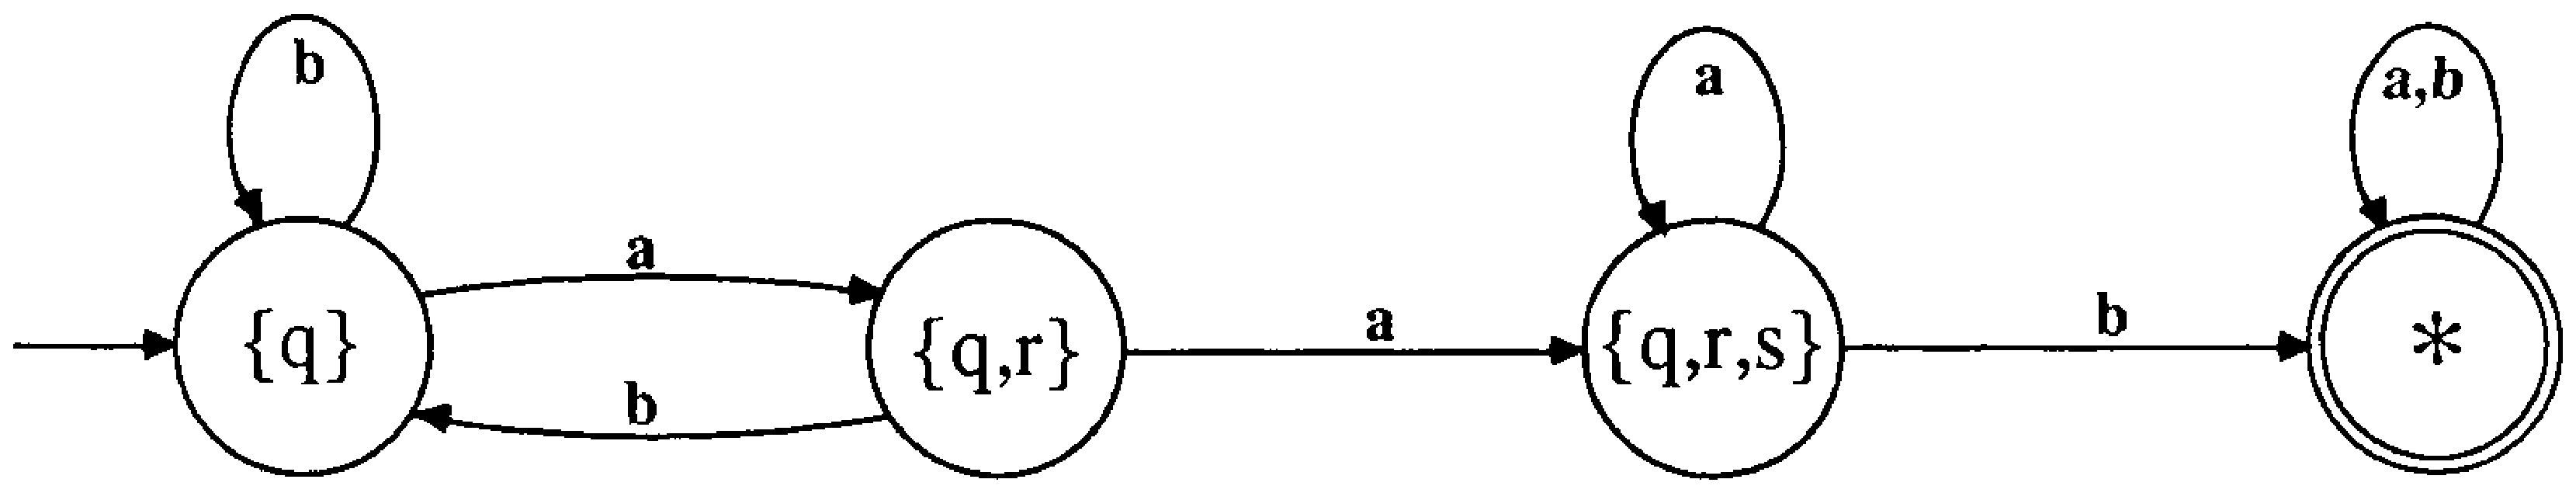
\epsfig{figure=ToFAfigures/fig4-15.eps,width=6.5in}}
\caption{A reduced equivalent of the DFA given in Figure \ref{fig-4.14}}\label{fig-4.15}
\end{figure}

The above process can be easily automated; an interesting but frustrating
exercise might involve producing an appropriate set of rules for generating,
given a specific string $y$, a DFA that will recognize all strings containing
the substring $y$. Definition \ref{dfn-4.5} can be used to generate the appropriate DFA
from the obvious NDFA without subjecting the designer to such frustrations!

\section{Circuit Implementation of NDFAs}\label{sec-4.2}

As mentioned earlier, the presence of multiple paths within an NDFA for a single
word characterizes the nondeterministic nature of these automata. The most
profitable way to view the operation of an NDFA is to consider the automaton as
having (potentially) several active states, with each of the active states
reacting to the next letter to determine a new set of active states. In fact, by
using one D flip-flop per state, this viewpoint can be directly translated into
hardware. When a given state is active, the corresponding flip-flop will be on,
and when it is inactive (that is, it cannot be reached by the substring that has
been processed at this point), it will be off. As a new letter is processed, a
state will be activated (that is, be placed in the new set of active states) if
it can be reached from one of the previously active states. Thus, the state
transition function will again determine the circuitry that feeds into each
flip-flop.

Following the same conventions given for DFAs, the input tape will be assumed
to be bounded by special start-of-string \<SOS\> and end-of-string \<EOS\>
symbols. The \<EOS\> character is again used to activate the accept circuitry
so that acceptance is not indicated until all letters on the tape have been
processed. As before, the \<SOS\> symbol can be employed at the beginning of the
string to ensure that the circuitry begins processing the string from the
appropriate start state(s). Alternately, SR (set-reset) flip-flops can be used
to initialize the configuration without relying on the <SOS> conventions.

\subsection*{Example 4.13}

Consider the NDFA $D$ given in Figure \ref{fig-4.16}. With the \<SOS\> and \<EOS\>
transitions illustrated, the complete model would appear as in Figure \ref{fig-4.17}.

Two bits of input data ($\pmb{a}_1$ and $\pmb{a}_2$) are required to represent
the symbols \<EOS\>, $\pmb{a}$, $\pmb{b}$, and \<SOS\>. The standard encodings
described in Chapter \ref{ch-1} would produce \<EOS\> $=\pmb{00},\pmb{a}=\pmb{01},\pmb{b}
=\pmb{10}$, and \<SOS\> $=\pmb{11}$. If the flip-flop $t_1$ is used to represent
the activity of $s_1$, and $t_2$ is used to record the status of $s_2$, then
the subsequent activity of the two flip-flops can be determined from the current
state activity and the current letter being scanned, as shown in Table \ref{tbl-4.1}.

% Figure 4.16
\begin{figure}
\centerline{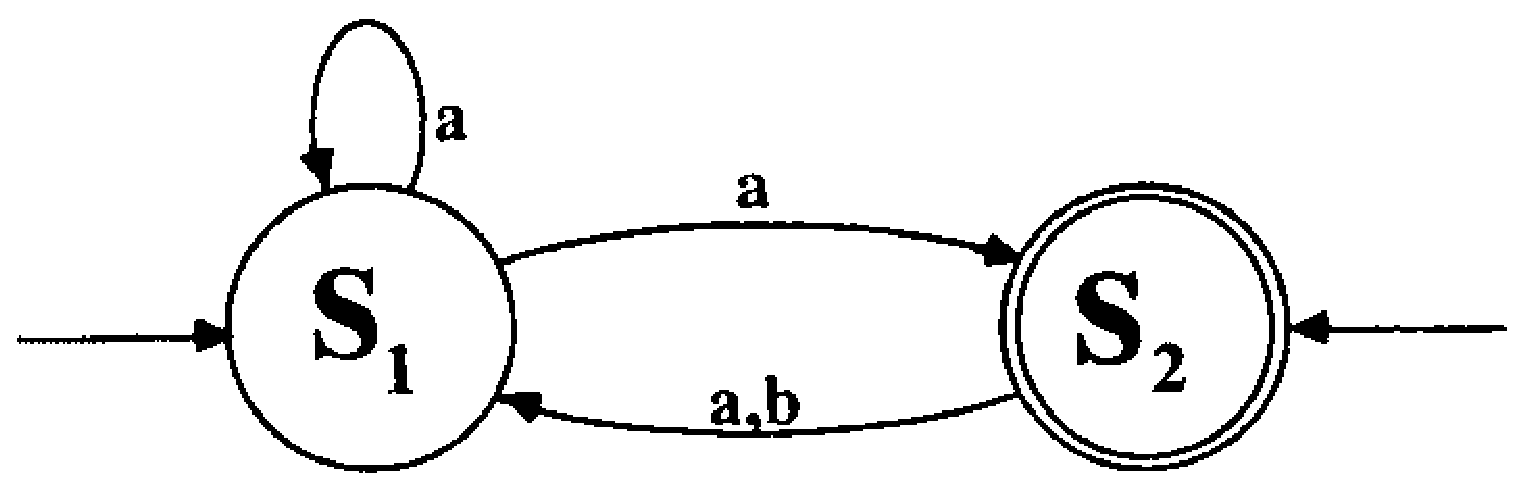
\epsfig{figure=ToFAfigures/fig4-16.eps,width=2.5in}}
\caption{The NDFA discussed in Example 4.13}\label{fig-4.16}
\end{figure}
% Figure 4.17
\begin{figure}
\centerline{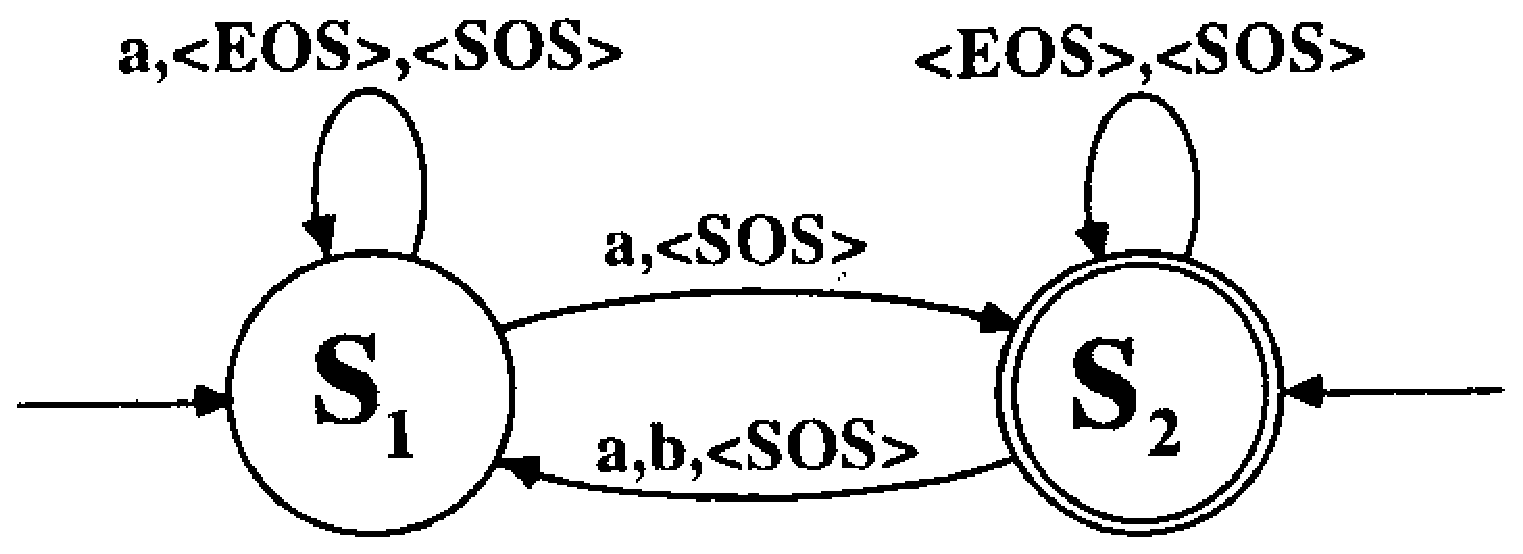
\epsfig{figure=ToFAfigures/fig4-17.eps,width=2.5in}}
\caption{The expanded state transition diagram for the NDFA in Figure \ref{fig-4.16}}\label{fig-4.17}
\end{figure}

% Table 4.1
\begin{table}[h]
\caption{}\label{tbl-4.1}
\begin{center}\begin{tabular}{cccc|ccc}
$t_1$ & $t_2$ & $a_1$ & $a_2$ & $t'_1$ & $t'_2$ & {\bf accept} \\
\hline
$\pmb{0}$ & $\pmb{0}$ & $\pmb{0}$ & $\pmb{0}$ & $\pmb{0}$ & $\pmb{0}$ &
	$\pmb{0}$ \\
$\pmb{0}$ & $\pmb{0}$ & $\pmb{0}$ & $\pmb{1}$ & $\pmb{0}$ & $\pmb{0}$ &
	$\pmb{0}$ \\
$\pmb{0}$ & $\pmb{0}$ & $\pmb{1}$ & $\pmb{0}$ & $\pmb{0}$ & $\pmb{0}$ &
	$\pmb{0}$ \\
$\pmb{0}$ & $\pmb{0}$ & $\pmb{1}$ & $\pmb{1}$ & $\pmb{1}$ & $\pmb{1}$ &
	$\pmb{0}$ \\
$\pmb{0}$ & $\pmb{1}$ & $\pmb{0}$ & $\pmb{0}$ & $\pmb{0}$ & $\pmb{1}$ &
	$\pmb{1}$ \\
$\pmb{0}$ & $\pmb{1}$ & $\pmb{0}$ & $\pmb{1}$ & $\pmb{1}$ & $\pmb{0}$ &
	$\pmb{0}$ \\
$\pmb{0}$ & $\pmb{1}$ & $\pmb{1}$ & $\pmb{0}$ & $\pmb{1}$ & $\pmb{0}$ &
	$\pmb{0}$ \\
$\pmb{0}$ & $\pmb{1}$ & $\pmb{1}$ & $\pmb{1}$ & $\pmb{1}$ & $\pmb{1}$ &
	$\pmb{0}$ \\
$\pmb{1}$ & $\pmb{0}$ & $\pmb{0}$ & $\pmb{0}$ & $\pmb{1}$ & $\pmb{0}$ &
	$\pmb{0}$ \\
$\pmb{1}$ & $\pmb{0}$ & $\pmb{0}$ & $\pmb{1}$ & $\pmb{1}$ & $\pmb{1}$ &
	$\pmb{0}$ \\
$\pmb{1}$ & $\pmb{0}$ & $\pmb{1}$ & $\pmb{0}$ & $\pmb{0}$ & $\pmb{0}$ &
	$\pmb{0}$ \\
$\pmb{1}$ & $\pmb{0}$ & $\pmb{1}$ & $\pmb{1}$ & $\pmb{1}$ & $\pmb{1}$ &
	$\pmb{0}$ \\
$\pmb{1}$ & $\pmb{1}$ & $\pmb{0}$ & $\pmb{0}$ & $\pmb{1}$ & $\pmb{1}$ &
	$\pmb{1}$ \\
$\pmb{1}$ & $\pmb{1}$ & $\pmb{0}$ & $\pmb{1}$ & $\pmb{1}$ & $\pmb{1}$ &
	$\pmb{0}$ \\
$\pmb{1}$ & $\pmb{1}$ & $\pmb{1}$ & $\pmb{0}$ & $\pmb{1}$ & $\pmb{0}$ &
	$\pmb{0}$ \\
$\pmb{1}$ & $\pmb{1}$ & $\pmb{1}$ & $\pmb{1}$ & $\pmb{1}$ & $\pmb{1}$ &
	$\pmb{0}$
\end{tabular}\end{center}
\end{table}

The first four rows of Table \ref{tbl-4.1} reflect the situation in which a string is
hopelessly stuck, and no states are active. Processing subsequent symbols from
$\Sigma$, will not change this; both $t'_1$ and $t'_2$ remain $\pmb{0}$. The one
exception is when the \<SOS\> symbol is scanned; in this case, each of the start
states is activated ($t'_1 = \pmb{1}$ and $t'_2 = \pmb{1}$). This corrects the
situation in which both flip-flops happen to initialize to $\pmb{0}$ when power
is first applied to the circuitry. Scanning the \<SOS\> symbol changes the state
of the flip-flops to reflect the appropriate starting conditions (in this
machine, both states are start states, and therefore both should be active as
processing is begun). Note that each of the rows of Table \ref{tbl-4.1} that correspond to
scanning \<SOS\> show that $t_1$ and $t_2$ are reset in the same fashion.

Determining the circuit behavior for the symbols in $\Sigma$, closely parallels
the definition of $\delta^d$ in Definition \ref{dfn-4.5}. For example, when state $s_1$ is
active but $s_2$ is inactive $(t_1=\pmb{1}$ and $t_2=\pmb{0})$ and $\pmb{a}$ is
scanned $(\pmb{a}_1=\pmb{0}$ and $\pmb{a}_2=\pmb{1})$, transitions from $s_1$
cause both states to next be active ($t'_1=\pmb{1}$ and $t'_2=\pmb{1}$). The
other combinations are calculated similarly. Minimized expressions for the new
values of each of the flip-flops and the accept circuitry are:
\begin{center}\begin{tabular}{rcl}
$t'_1$ & $=$ & $(t_1\wedge\neg\pmb{a}_1) \vee (t_2\wedge\pmb{a}_2) \vee
	(t_2\wedge\pmb{a}_1) \vee (\pmb{a}_1\wedge\pmb{a}_2)$ \\
$t'_2$ & $=$ & $(t_2\wedge\neg\pmb{a}_1\wedge\neg\pmb{a}_2) \vee
	(t_1\wedge\pmb{a}_2) \vee (\pmb{a}_1\wedge\pmb{a}_2)$ \\
accept & $=$ & $(t_2\wedge\neg\pmb{a}_1\wedge\neg\pmb{a}_2)$
\end{tabular}\end{center}
Since similar terms appear in these expressions, these three subcircuits can
``share'' the common components, as shown in Figure \ref{fig-4.18}.

% Figure 4.18
\begin{figure}
\centerline{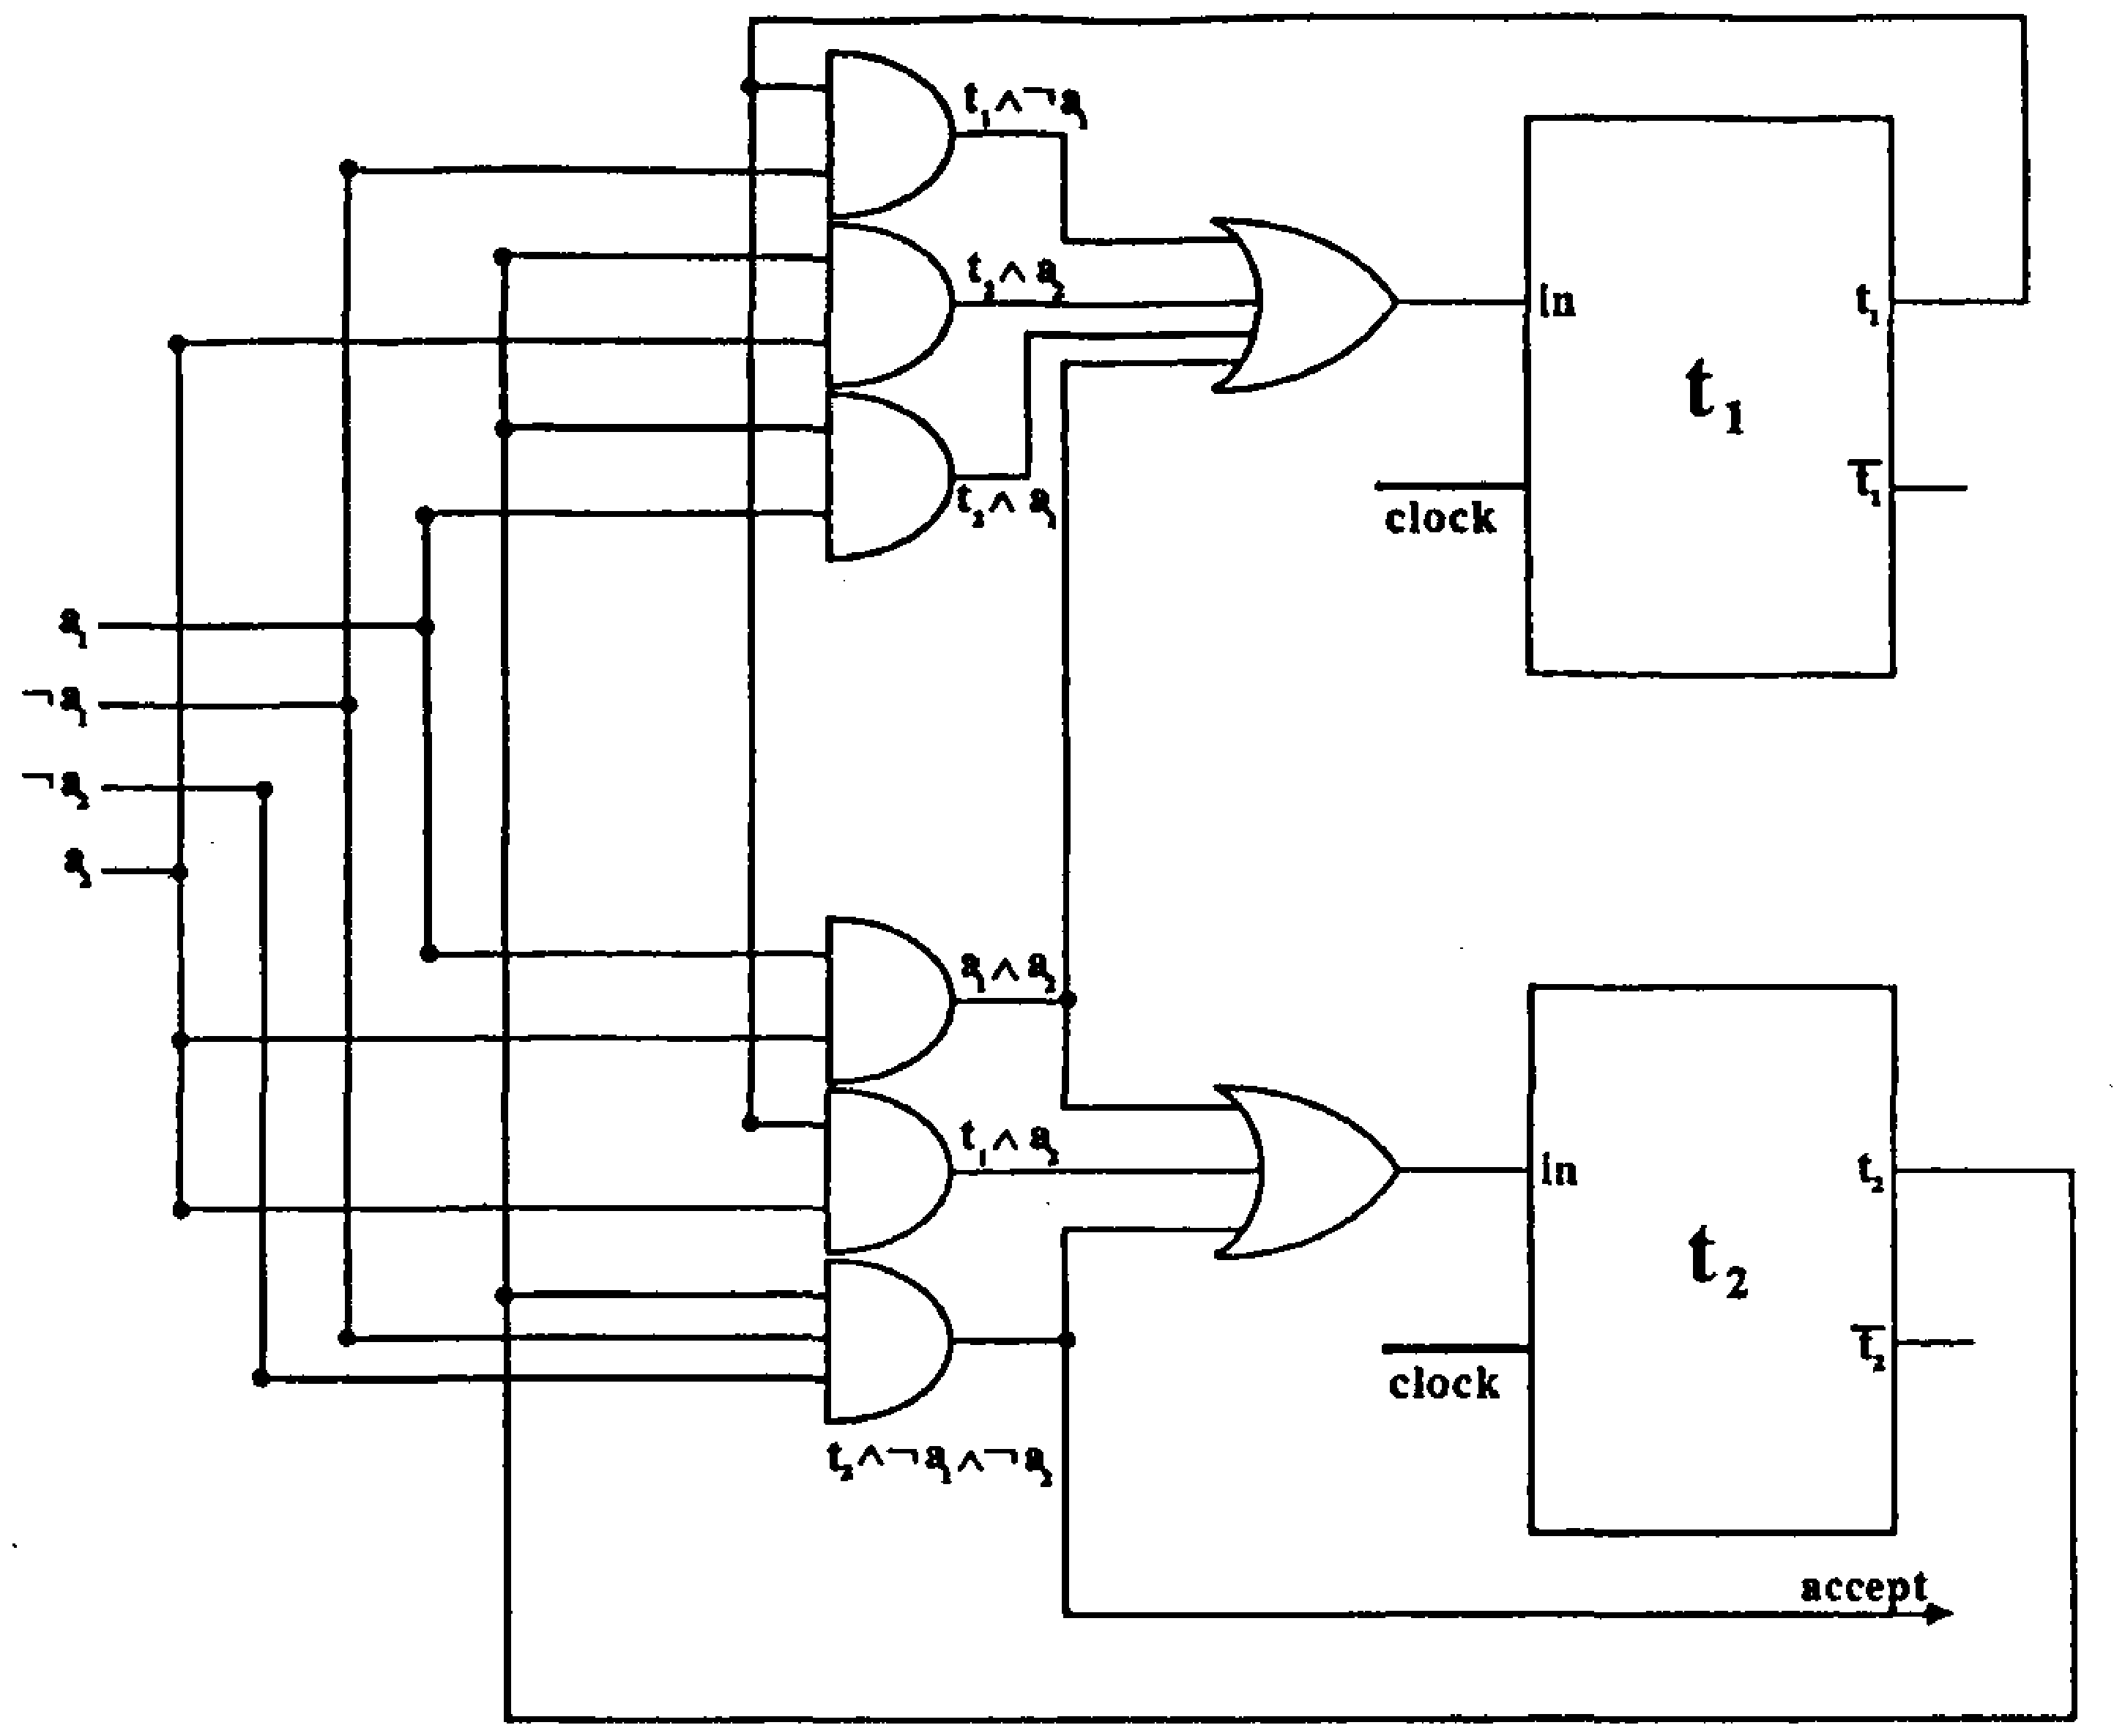
\epsfig{figure=ToFAfigures/fig4-18.eps,width=6in}}
\caption{Circuitry for the automaton discussed in Example 4.13}\label{fig-4.18}
\end{figure}

Note that the accept circuitry reflects that a string should be recognized when
some final state is active ($s_2$ in this example) and \<EOS\> is scanned. In
more complex machines with several final states, lines leading from each of the
flip-flops corresponding to final states would be joined by an OR gate
before being ANDed with the \<EOS\> condition.

An interesting exercise involves converting the NDFA $D$ given in Example 4.1
to the equivalent DFA $D^d$, which will have four states: $\emptyset,\ \{s_1\},\
\{s_2\}$, and $\{s_1,s_2\}$. The deterministic automaton $D^d$ can be realized
by a circuit diagram as specified in Chapter \ref{ch-1}. This four-stare DFA will require
2 bits of state data. If the state encoding conventions $\emptyset=\pmb{00}$,
$\{s_1\}=\pmb{10}$, $\{s_2\}=\pmb{01}$, and $\{s_1,s_2\}=\pmb{11}$ are used, the
circuitry for the DFA $D^d$ will be identical to that for the NDFA $D$.

For DFAs, $m$ bits of state data ($t_1,t_2, \ldots ,t_m)$ can encode up to $2^m$
distinct states. With NDFAs, an $n$-state machine required a full $n$ bits of
state data (1 bit per state). This apparently ``extravagant'' use of state data
is offset by the fact that an $n$-state NDFA may require $2^n$ states to form an
equivalent DFA. This was the case in the preceding example, in which $n$ and $m$
were equal to 2; the two-state NDFA $D$ required two flip-flops, and the
equivalent four-state DFA also required two flip-flops; the savings induced by
the DFA state encoding was exactly offset by the multiplicity of states needed
by the NDFA.

A DFA may turn out to need less hardware than an equivalent NDFA, as illustrated
by Example 4.12. The four-state NDFA $C$ needs four flip-flops, and the
(nonminimal, 16-state) DFA $C^d$ would also need four. However, the minimal
equivalent DFA derived in Example 4.12 has only four states and therefore can be
encoded with just 2 bits of state data. Hence only two flip-flops are necessary
to implement a recognizer for $L(C)$.

\section{NDFAs With Lambda-Transitions}\label{sec-4.3}

We now extend our computational model to include the nondeterministic finite
automata that allow transitions between states to occur ``spontaneously,''
without any input being processed. A transition that occurs without an input
symbol being processed is called a \emph{$\lambda$-transition} or
\emph{lambda-move}\index{lambda-move|see|{$\lambda$-transition}}. In texts that denote the empty string by the symbol
$\epsilon$, such a transition is usually referred to as an
\emph{$\epsilon$-move}\index{$\epsilon$-move|see{$\lambda$-transition}}.

% Definition 4.6
\begin{dfn}\label{dfn-4.6}\index{L@$\lambda$-transition}
A \emph{nondeterministic finite automaton with $\lambda$-transitions} is a
quintuple $A_{\lambda}=\langle\Sigma,S,S_0,\delta_{\lambda},F\rangle$, where
\begin{enumerate}[i.]
\item $\Sigma$ is an alphabet.
\item $S$ is a finite nonempty set of states.
\item $S_0$ is a set of initial states,\index{start state} a nonempty subset of $S$.
\item $\delta_{\!\lambda}:\ (S \times (\Sigma\cup\{\lambda\})) \rightarrow \wp(S)$
	is the state transition function.
\item $F$ is the set of accepting states, a (possibly empty) subset of $S$.
\end{enumerate}
\end{dfn}

A nondeterministic finite automaton \emph{with} $\lambda$-transitions is very
similar in structure to an NDFA that does not have $\lambda$-transitions. The
only different aspect is the definition of the $\delta$ function. Instead of
mapping state/letter pairs [from $S \times \Sigma$] to $\wp(S)$, it maps pairs
consisting of a state and either a letter or the empty string [from $S \times
(\Sigma\cup\{\lambda\})$ to $\wp(S)$]. From any state that has a
$\lambda$-transition, we adopt the convention that the machine is capable of
making a spontaneous transition to the new state specified by that
$\lambda$-transition \emph{without} processing an input symbol. However, the
machine may also ``choose'' not to follow this path and instead remain in the
original state. Before we can extend the $\delta_{\lambda}$ function to operate
on strings from $\Sigma^*$, we need the very useful concept of
\emph{lambda-closure}\index{lambda-closure|see{$\lambda$-closure}}.

% Definition 4.7
\begin{dfn}\label{dfn-4.7}\index{L@$\lambda$-closure}
Given a nondeterministic finite automaton
\[ A_{\lambda} = \langle\Sigma,S,S_0,\delta_{\lambda},F\rangle \]
with $\lambda$-transitions, the \emph{$\lambda$-closure of a state} $t \in S$,
denoted $\Lambda(t)$, is the set of all states that are reachable from $t$
without processing any input symbols. The \emph{$\lambda$-closure of a
set of states $T$} is then $\Lambda(T) = \bigcup\limits_{t\,\in\, T} \Lambda(t)$.
\end{dfn}

The $\lambda$-closure of a state is the set of all the states that can be
reached from that state, including itself, by following $\lambda$-transitions only.
Obviously, one can always reach the state currently occupied without having to
move. Consequently, even if there are no explicit arcs labeled by $\lambda$
going back to state $t$, $t$ is always in the $\lambda$-closure of itself.

\subsection*{Example 4.14}

Consider the machine given in Figure \ref{fig-4.19}, which contains $\lambda$-transitions
from $s_0$ to $s_1$ and from $s_1$ to $s_2$. By Definition \ref{dfn-4.7},
\begin{center}\begin{tabular}{l}
$\Lambda(s_0) = \{s_0,s_1,s_2\}$ \\
$\Lambda(s_1) = \{s_1,s_2\}$ \\
$\Lambda(s_2) = \{s_2\}$ \\
$\Lambda(s_3) = \{s_3\}$
\end{tabular}\end{center}

% Figure 4.19
\begin{figure}
\centerline{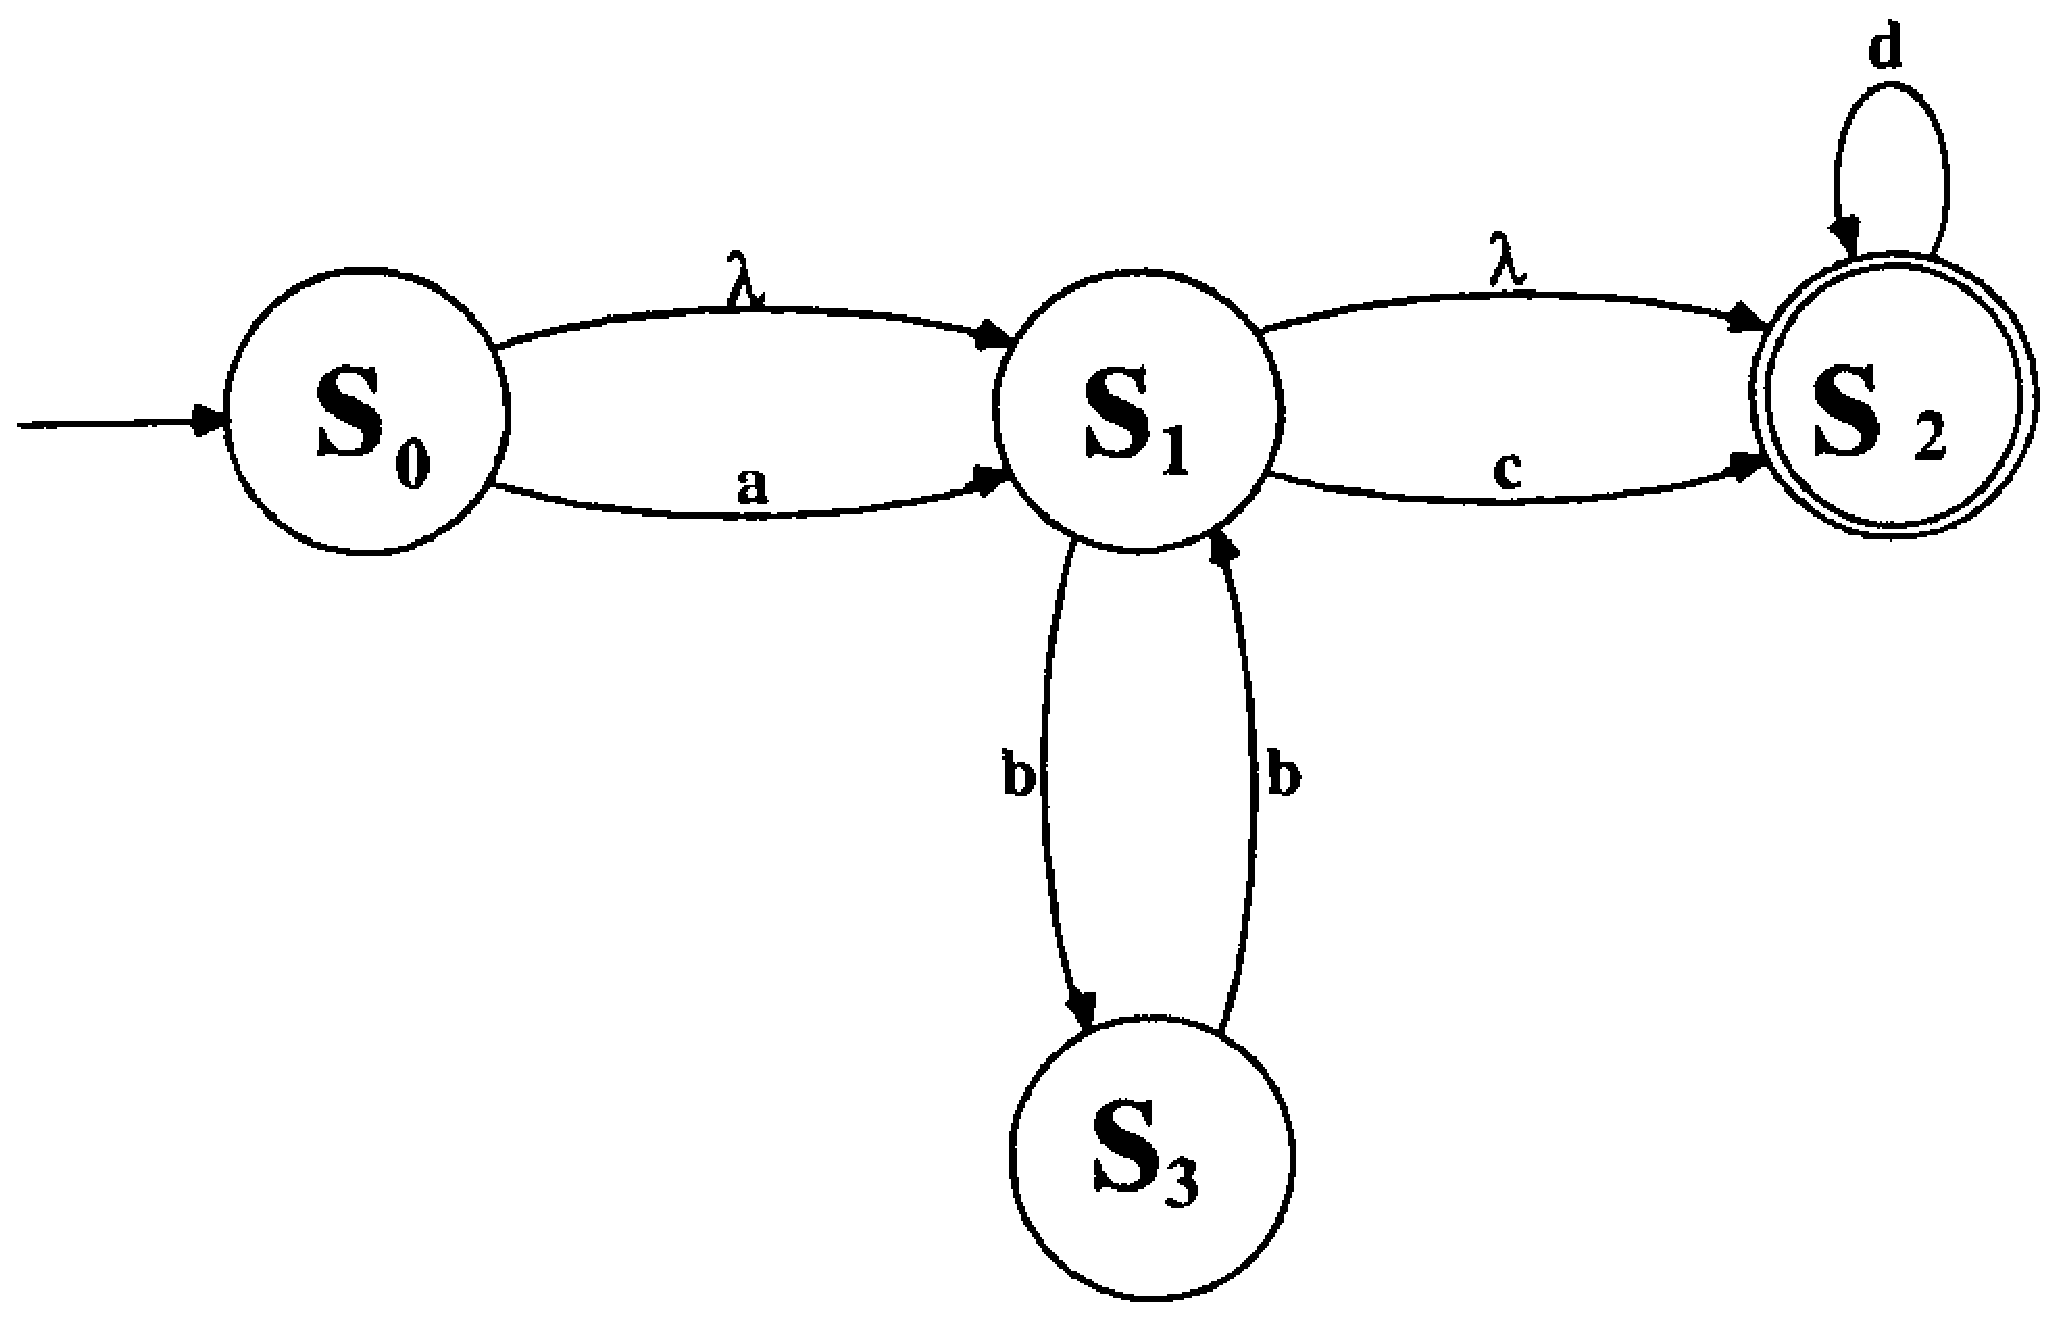
\epsfig{figure=ToFAfigures/fig4-19.eps,width=3.5in}}
\caption{An NDFA with lambda-moves}\label{fig-4.19}
\end{figure}

% Definition 4.8
\begin{dfn}\label{dfn-4.8}\index{extended state transition function \DBAR\! for NDFA $A_{\lambda}$}\index{state transition function!for NDFA $A_{\lambda}$}
Given a nondeterministic finite automaton
\[ A_{\lambda} = \langle\Sigma,S,S_0,\delta_{\lambda},F\rangle \]
with $\lambda$-transitions, the \emph{extended state transition function
for $A_{\lambda}$} is a function $\DBAR_{\!\lambda}$$: S \times \Sigma^*
\rightarrow \wp(S)$ defined as follows:
\begin{enumerate}[i.]
\item $(\forall s \in S)\DBAR_{\!\lambda}(s,\lambda) = \Lambda(s)$
\item $(\forall s \in S)(\forall\pmb{a}\in\Sigma)\DBAR_{\!\lambda}(s,\pmb{a}) =
	\Lambda( \bigcup\limits_{q\,\in\,\Lambda(s)}\delta_{\!\lambda}(q,\pmb{a}))$
\item $(\forall s \in S)(\forall x \in \Sigma^*)(\forall\pmb{a}\in\Sigma)
	\DBAR_{\!\lambda}(s,x\pmb{a}) = \Lambda(\bigcup\limits_{q\,\in\,\DBAR_{
	\!\lambda}(s,x)} \delta_{\!\lambda}(q,\pmb{a}))$
\end{enumerate}
\end{dfn}

The $\DBAR_{\!\lambda}$ function is \emph{not} extended in the same way as for the
nondeterministic finite automata given in Definition \ref{dfn-4.2}. Most importantly, due
to the effects of the $\lambda$-closure, $\DBAR_{\!\lambda}(s,\pmb{a}) \not=
\delta_{\!\lambda}(s,\pmb{a})$. Thus, not only does the $\DBAR_{\!\lambda}$ function
map to a set of states based on a single letter, but it also includes the
$\lambda$-closure of those states. This may seem strange for single letters
(strings of length 1), but it is required for consistency when the
$\DBAR_{\!\lambda}$ function is presented with strings of length greater than 1,
since at each state along the path there can be $\lambda$-transitions. Each
$\lambda$-transition maps to a new state (which may have $\lambda$-transitions
of its own) that must be included in this path and processed by the
$\delta_{\!\lambda}$ function.

The nondeterministic finite automaton \emph{without} $\lambda$-transitions that
corresponds to a nondeterministic finite automaton \emph{with} $\lambda$-transitions is
given in Definition \ref{dfn-4.9}.

% Figure 4.20
\begin{figure}
\centerline{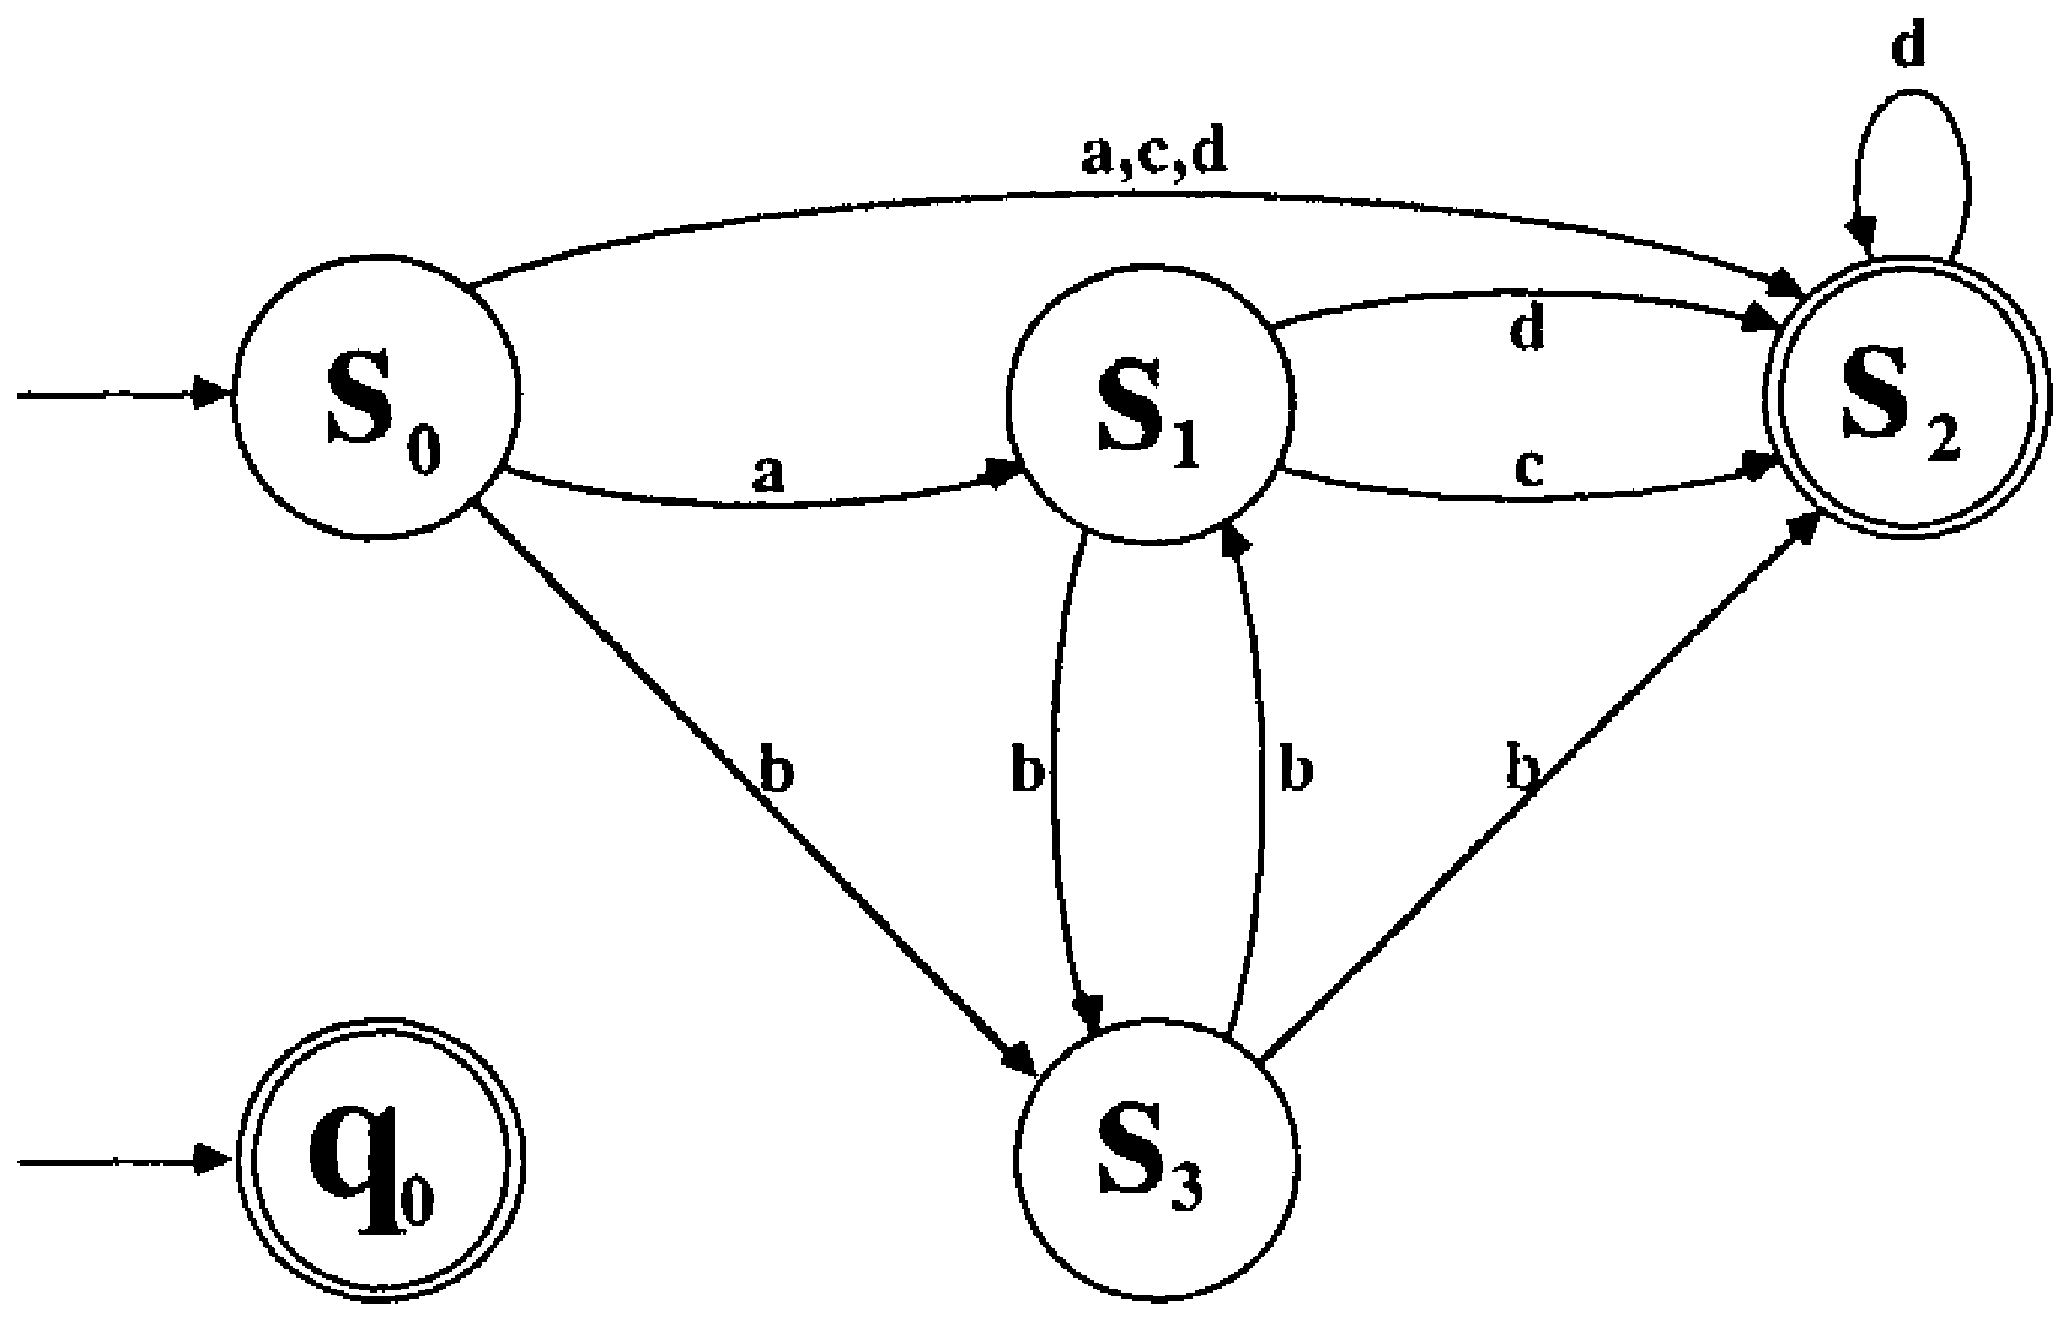
\epsfig{figure=ToFAfigures/fig4-20.eps,width=3.5in}}
\caption{An NDFA without lambda-moves that is equivalent to the automaton in
Figure \ref{fig-4.19}}\label{fig-4.20}
\end{figure}

% Definition 4.9
\begin{dfn}\label{dfn-4.9}
Given a nondeterministic finite automaton \emph{with} $\lambda$-transitions,
$A_{\lambda}=\langle\Sigma,S,S_0,\delta_{\lambda},F\rangle$, the
\emph{corresponding nondeterministic finite automaton without
$\lambda$-transitions}, $A^{\sigma}_{\lambda}=\langle\Sigma,S\cup\{q_0\},S_0\cup
\{q_0\},\delta^{\sigma}_{\lambda},F^{\sigma}\rangle$, is defined as follows:

\begin{center}\begin{tabular}{l}
$F^{\sigma} = \left\{ \begin{tabular}{ll}
		$F$ & $\quad\text{iff}\quad\lambda\notin L(A_{\lambda})$ \\
 		$F \cup \{q_0\}$ & $\quad\text{iff}\quad \lambda\in
			L(A_{\lambda})$
		\end{tabular}\right. $ \\
$(\forall\pmb{a}\in\Sigma)\delta^{\sigma}_{\lambda}(q_0,\pmb{a}) = \emptyset$ \\
$(\forall s \in S)(\forall\pmb{a}\in\Sigma)\quad \delta^{\sigma}_{\lambda}(s,
	\pmb{a}) = \DBAR_{\!\lambda}(s,\pmb{a}) =
        \Lambda(\bigcup\limits_{q\,\in\,\Lambda(s)}\delta_{\lambda}
	(q,\pmb{a}))$
\end{tabular}\end{center}
and which is extended in the ``usual'' way for nondeterministic finite automata
to the function \linebreak$\overline{\delta^{\sigma}_{\lambda}}$$: (S \cup \{q_0\}) \times \Sigma^*
\rightarrow \wp(S \cup \{q_0\})$.
\end{dfn}

Note that from a state in $A_{\lambda}$ several $\lambda$-transitions may be
taken, then a single letter $\pmb{a}$ may be processed, and then several more
$\lambda$-moves may occur; all this activity can result from just a single
symbol on the input tape being processed. The definition of
$\delta^{\sigma}_{\lambda}$ reflects these types of transitions. The
$\delta^{\sigma}_{\lambda}$ function is defined to be the same as the
$\DBAR_{\lambda}$ function for all single letters (strings of length 1), which
adjusts for the $\lambda$-closure of $A_{\lambda}$. The
$\delta^{\sigma}_{\lambda}$ function can then be extended in the usual
nondeterministic manner.

To account for the case that $\lambda$ might be in the language accepted by the
automaton $A_{\lambda}$, we add an extra start state $q_0$ to the corresponding
machine $A^{\sigma}_{\lambda}$, which is disconnected from the rest of the
machine. If $\lambda\in L(A_{\lambda})$, we also make $q_0$ a final state.

\subsection*{Example 4.15}

Let $A_{\lambda}$ represent the NDFA given in Example 4.14. $A^{\sigma}_{\lambda}$ would
then be given by the NDFA shown in Figure \ref{fig-4.20}. This new NDFA does indeed accept
the same language as $A_{\lambda}$. To show in general that $L(A_{\lambda}) =
L(A^{\sigma}_{\lambda})$, we must first show that the respective extended state
transition functions behave in similar fashions. However, these two functions
can be equivalent only for strings of nonzero length (because of the effects of
the $\lambda$-closure in the definition of $\delta^{\sigma}_{\lambda}$). This
result is established in Lemma \ref{lmm-4.2}.

% Lemma 4.2
\begin{lmm}\label{lmm-4.2}
Given a nondeterministic finite automaton $A_{\lambda}$ \emph{with}
$\lambda$-transitions and the corresponding nondeterministic finite automaton
$A^{\sigma}_{\lambda}$ \emph{without} $\lambda$-transitions, then
\[ (\forall s \in S)(\forall x \in \Sigma^+)(\overline{\delta^{\sigma}_{\lambda}}(s,x) =
	\DBAR_{\lambda}(s,x)) \]
\emph{Proof.} The proof is by induction on $|x|$; see the exercises.
\end{lmm}

Once we have shown that the extended state transition functions behave
(almost) identically, we can proceed to show that the languages accepted by
these two machines are the same.

% Theorem 4.2
\begin{thm}\label{thm-4.2}\index{equivalent!NDFAs}
Given a nondeterministic finite automaton that contains $\lambda$-transitions,
there exists an \emph{equivalent} nondeterministic finite automaton that does
not have $\lambda$-transitions.

\emph{Proof.} Assume $A_{\lambda}=\langle\Sigma,S,S_0,\delta_{\lambda},F\rangle$
is an NDFA with $\lambda$-transitions. Construct the corresponding NDFA
$A^{\sigma}_{\lambda} = \langle\Sigma,S\cup\{q_0\},S_0\cup\{q_0\},
\delta^{\sigma}_{\lambda},F^{\sigma}\rangle$, which has no $\lambda$-transitions.
We will show $L(A_{\lambda})=L(A^{\sigma}_{\lambda})$, and thereby prove that the
two machines are equivalent. Because the way $A^{\sigma}_{\lambda}$ was constructed
limits the scope of Lemma \ref{lmm-4.2}, the proof is divided into two cases.

{\bf Case 1}: If $x = \lambda$, then by Definition \ref{dfn-4.9}
\[ (q_0 \in F^{\sigma}\text{ iff }\lambda \in L (A_{\lambda})) \]
and so
\[ (\lambda \in L(A^{\sigma}_{\lambda}) \Leftrightarrow \lambda \in
	L(A_{\lambda})) \]

{\bf Case 2}: Assume $x \neq \lambda$. Since there are no transitions leaving
$q_0$, it may be disregarded as one of the start states of $A^{\sigma}_{\lambda}$. Then
\begin{center}\begin{tabular}{rcl}
$x \in L(A^{\sigma}_{\lambda})$ & $\Rightarrow$ & (by definition of $L$) \\
$(\bigcup\limits_{s_0\,\in\, S_0}\overline{\delta^{\sigma}_{\lambda}}(s_0,x)) \cap F^{\sigma}
	\not=\emptyset$ & $\Rightarrow$ & (by Lemma \ref{lmm-4.2}) \\
$(\bigcup\limits_{s_0\,\in\, S_0}\DBAR_{\lambda}(s_0,x)) \cap F^{\sigma} \not=
	\emptyset$ & $\Rightarrow$ & \begin{tabular}{l}(since if $q_0$ were the
	common element, then $x$ \\ would have to be $\lambda$, which violates
	the assumption) \end{tabular} \\
$(\bigcup\limits_{s_0\,\in\, S_0}\DBAR_{\lambda}(s_0,x)) \cap F \not= \emptyset$
	& $\Rightarrow$ & (by definition of $L$)
\\$x \in L(A_{\lambda})$
\end{tabular}\end{center}
Conversely, and for many of the same reasons, we have
\begin{center}\begin{tabular}{rcl}
$x \in L(A_{\lambda})$ & $\Rightarrow$ & (by definition of $L$) \\
$(\bigcup\limits_{s_0\,\in\, S_0}\DBAR_{\lambda}(s_0,x)) \cap F \not= \emptyset$
	& $\Rightarrow$ & (by Lemma \ref{lmm-4.2}) \\
$(\bigcup\limits_{s_0\,\in\, S_0}\overline{\delta^{\sigma}_{\lambda}}(s_0,x)) \cap F
	\not=\emptyset$ & $\Rightarrow$ & (since $F \subseteq F^{\sigma}$) \\
$(\bigcup\limits_{s_0\,\in\, S_0}\overline{\delta^{\sigma}_{\lambda}}(s_0,x)) \cap F^{\sigma}
	\not=\emptyset$ & $\Rightarrow$ & (by definition of $L$) \\
$x \in L(A^{\sigma}_{\lambda})$ &&
\end{tabular}\end{center}
Consequently, $(\forall x \in \Sigma^*)(x \in L(A^{\sigma}_{\lambda})
\Leftrightarrow x \in L(A_{\lambda}))$.
\end{thm}

Although nondeterministic finite automata \emph{with} $\lambda$-transitions are
no more powerful than nondeterministic finite automata \emph{without}
$\lambda$-transitions and consequently recognize the same class of languages as
deterministic finite automata, they have their place in theory and machine
construction. Because such machines can be constructed very easily from
\emph{regular expressions} (see Chapter \ref{ch-6}), NDFAs are used by the
UNIX$^{\text{TM}}$ text editor and by lexical analyzer generators such as LEX for
pattern-matching applications. Example 4.16 involves the regular expression
$(\pmb{a}\cup\pmb{c})^*\pmb{bc}(\pmb{a}\cup\pmb{c})^*$, which describes the set
of words composed of any number of $\pmb{a}$s and $\pmb{c}$s, followed by a single
$\pmb{b}$, followed by a single $\pmb{c}$, followed by any number of $\pmb{a}$s and
$\pmb{c}$s.

\subsection*{Example 4.16}

Suppose that we wanted to construct a machine that will accept the language
$L=\{x \in \{\pmb{a},\pmb{b},\pmb{c}\}^*|x$ contains exactly one $\pmb{b}$, which
is immediately followed by $\pmb{c}\}$. A machine that accepts this language is
given in Figure \ref{fig-4.21}.

% Figure 4.21
\begin{figure}
\centerline{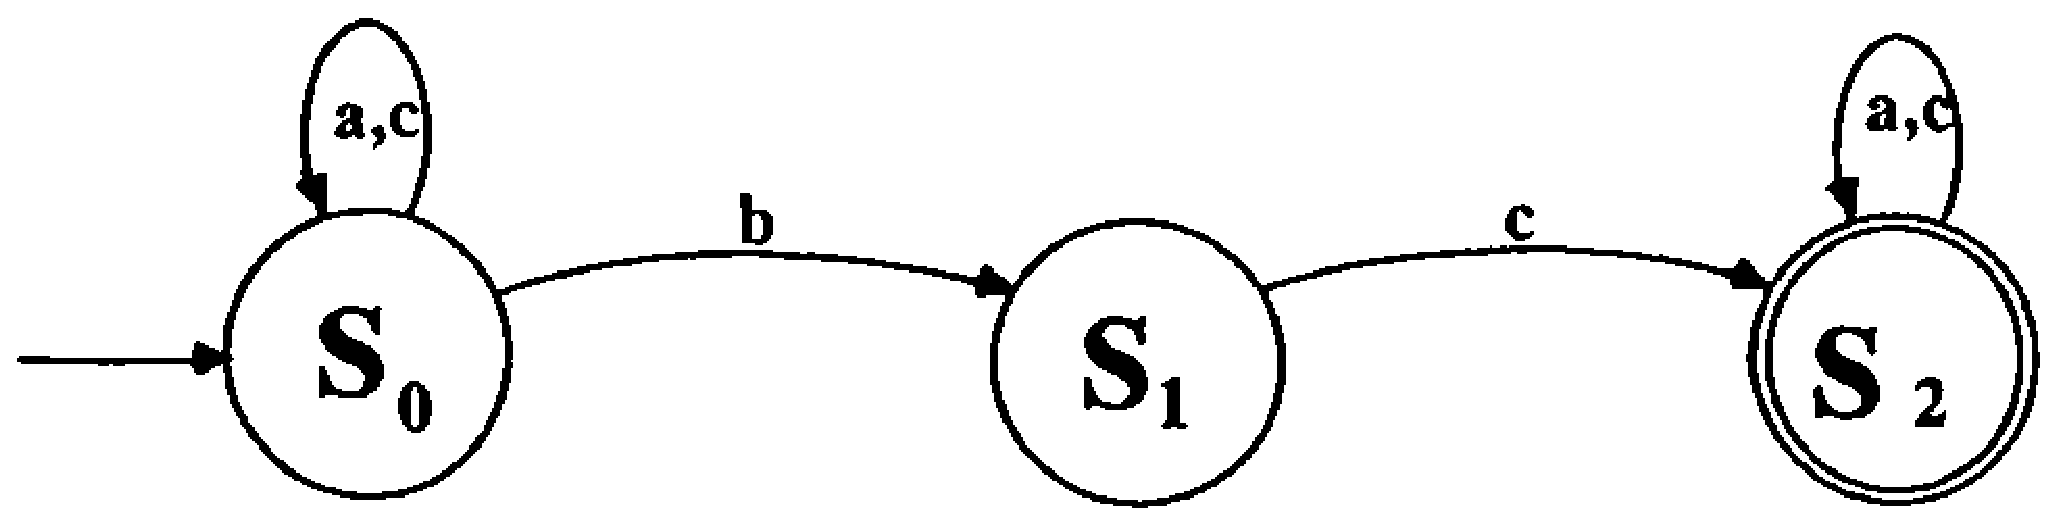
\epsfig{figure=ToFAfigures/fig4-21.eps,width=3.0in}}
\caption{The NDFA described in Example 4.16}\label{fig-4.21}
\end{figure}

Suppose we now wish to build a machine that will accept any positive number of
occurrences of various strings from this language concatenated together. In this
case, the resulting language would include all strings (with at least one $\pmb{
b}$) with the property that each and every $\pmb{b}$ is immediately followed by
$\pmb{c}$. By simply adding a $\lambda$-transition from every final state to the
start state, we achieve our objective. The machine that accepts this new
language is shown in Figure \ref{fig-4.22}.

% Figure 4.22
\begin{figure}
\centerline{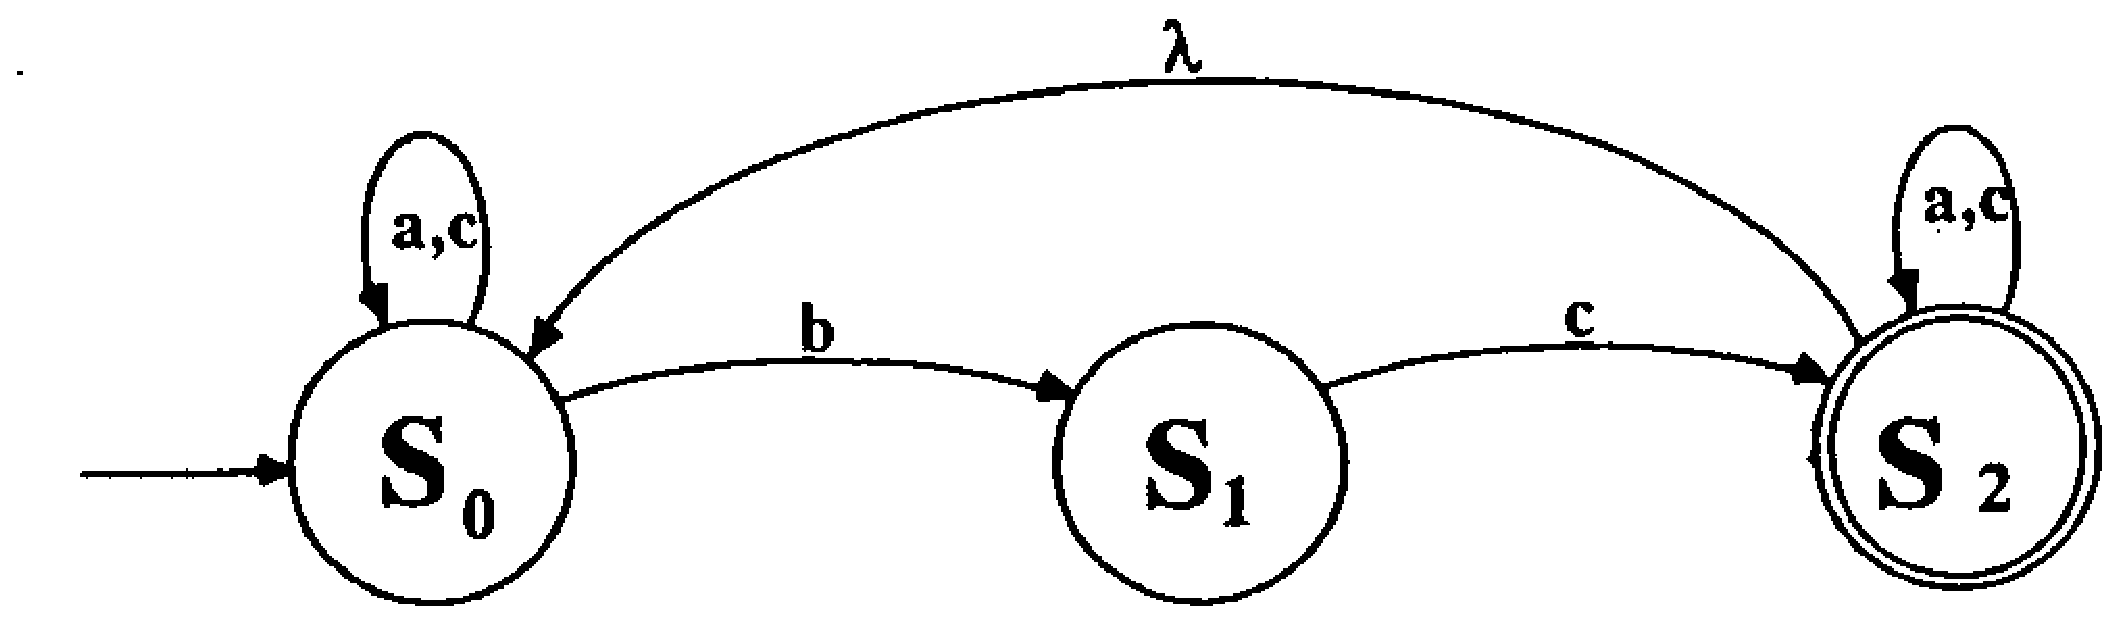
\epsfig{figure=ToFAfigures/fig4-22.eps,width=3.0in}}
\caption{The modification of the NDFA in Figure \ref{fig-4.21}}\label{fig-4.22}
\end{figure}

The previous section outlined how to implement nondeterministic finite automata
\emph{without} $\lambda$-transitions; accommodating $\lambda$-moves is in fact
quite straightforward. A $\lambda$-transition from state $s$ to state $t$
indicates that state $t$ should be considered active whenever state $s$ is
active. This can be assured by an obvious modification, as shown by the
following example.

% Figure 4.23
\begin{figure}
\centerline{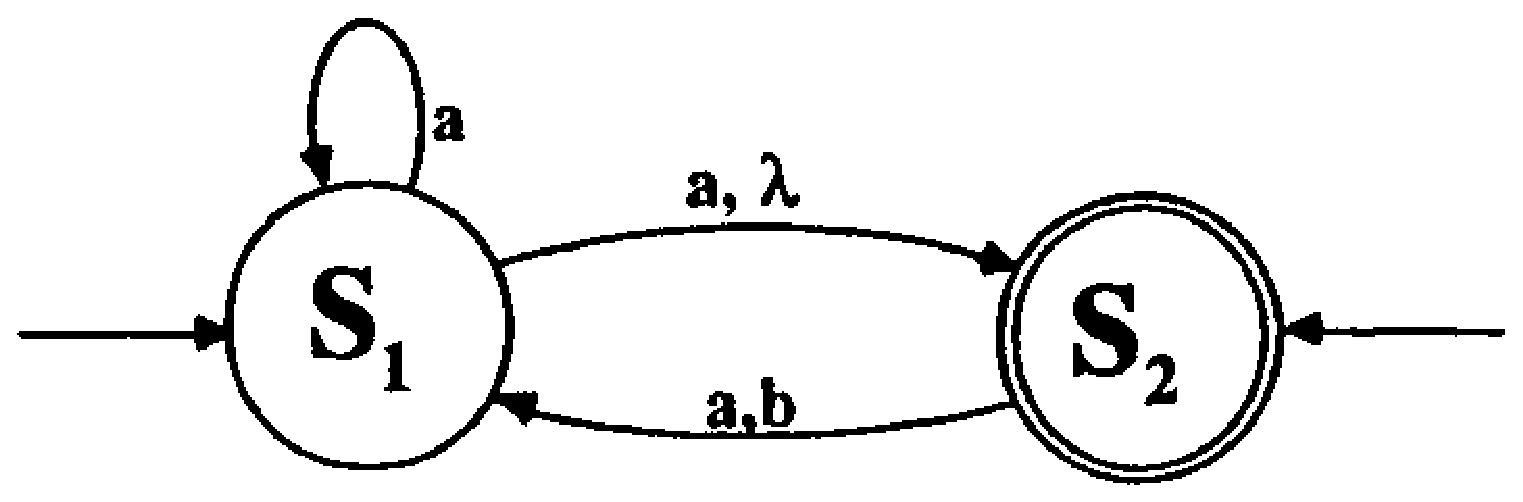
\epsfig{figure=ToFAfigures/fig4-23.eps,width=3.0in}}
\caption{A simple NDFA with lambda moves}\label{fig-4.23}
\end{figure}

\subsection*{Example 4.17}

As an illustration of how circuitry can be defined for machines with
$\lambda$-transitions, consider the DFA $E$ given in Figure \ref{fig-4.23}. This machine
is similar to the NDFA $D$ in Example 4.13, but a $\lambda$-transition has been
added from $s_1$ to $s_2$; that is, $\delta(s_1,\lambda)=\{s_2\}$. This
transition implies that $s_2$ should be considered active whenever $s_1$ is
active. Consequently, the circuit diagram produced in Example 4.13 need only be
slightly modified by establishing the extra connection indicated by the dotted
line shown in Figure \ref{fig-4.24}.

In general, the need for such ``extra'' connections leaving a given flip-flop
input $t_i$ is determined by examining $\delta(s_i,\lambda)$, the set of
$\lambda$-transitions for $s_i$. Note that the propagation delay in this circuit
has been increased; there are signals that must now propagate through an extra
gate during a single clock cycle. The delay will be exacerbated in automata that
contain sequences of $\lambda$-transitions. In such cases, the length of the
clock cycle may need to be increased to ensure proper operation. This problem
can be minimized by adding all the connections indicated by $\Lambda(s_i)$,
rather than just adding those implied by $\delta(s_i,\lambda)$.

% Figure 4.24
\begin{figure}
\centerline{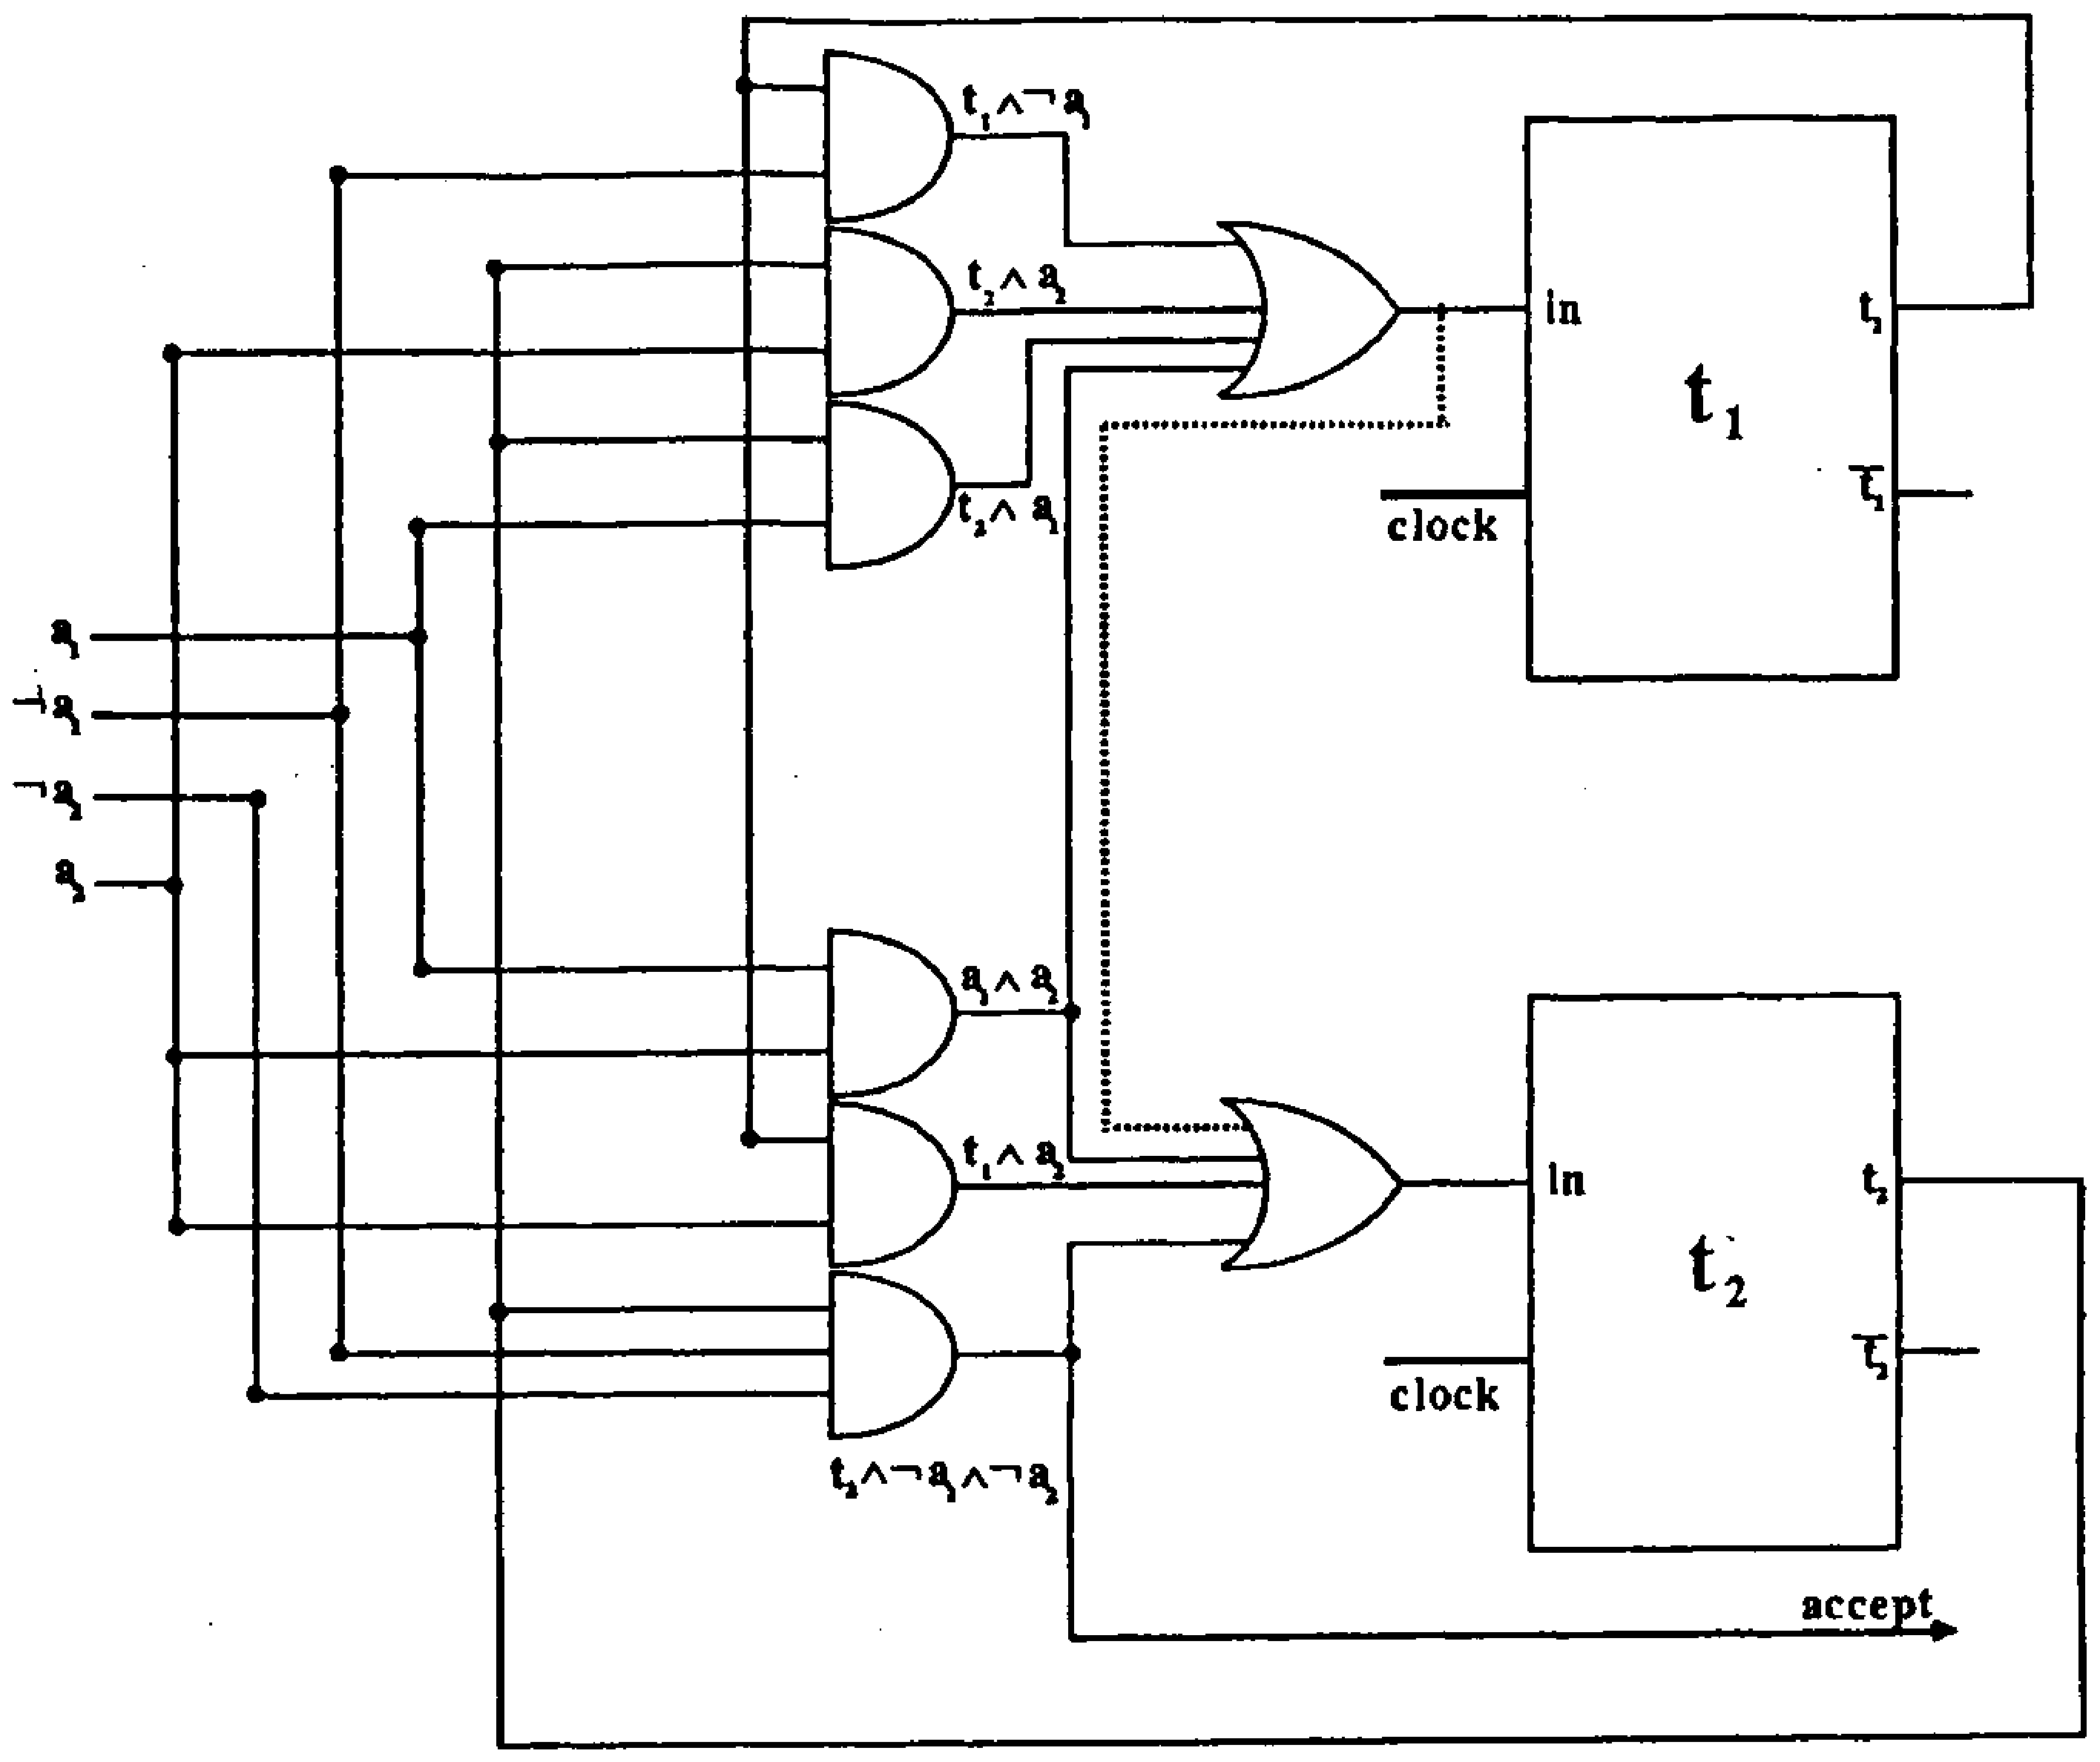
\epsfig{figure=ToFAfigures/fig4-24.eps,width=6.0in}}
\caption{Circuitry for the automaton discussed in Example 4.17}\label{fig-4.24}
\end{figure}

\section*{Exercises}
\begin{enumerate}[{4.}1.]
\item Draw the deterministic versions of each of the nondeterministic finite
automata shown in Figure \ref{fig-4.25}. In each part, assume $\Sigma=\{\pmb{a},\pmb{b},
\pmb{c}\}$.

\item Consider the automaton given in Example 4.17.
\begin{enumerate}
\item Convert this automaton into an NDFA without $\lambda$-transitions using
Definition \ref{dfn-4.9}.
\item Convert this NDFA into a DFA using Definition \ref{dfn-4.5}.
\end{enumerate}

% Figure 4.25
\begin{figure}
\centerline{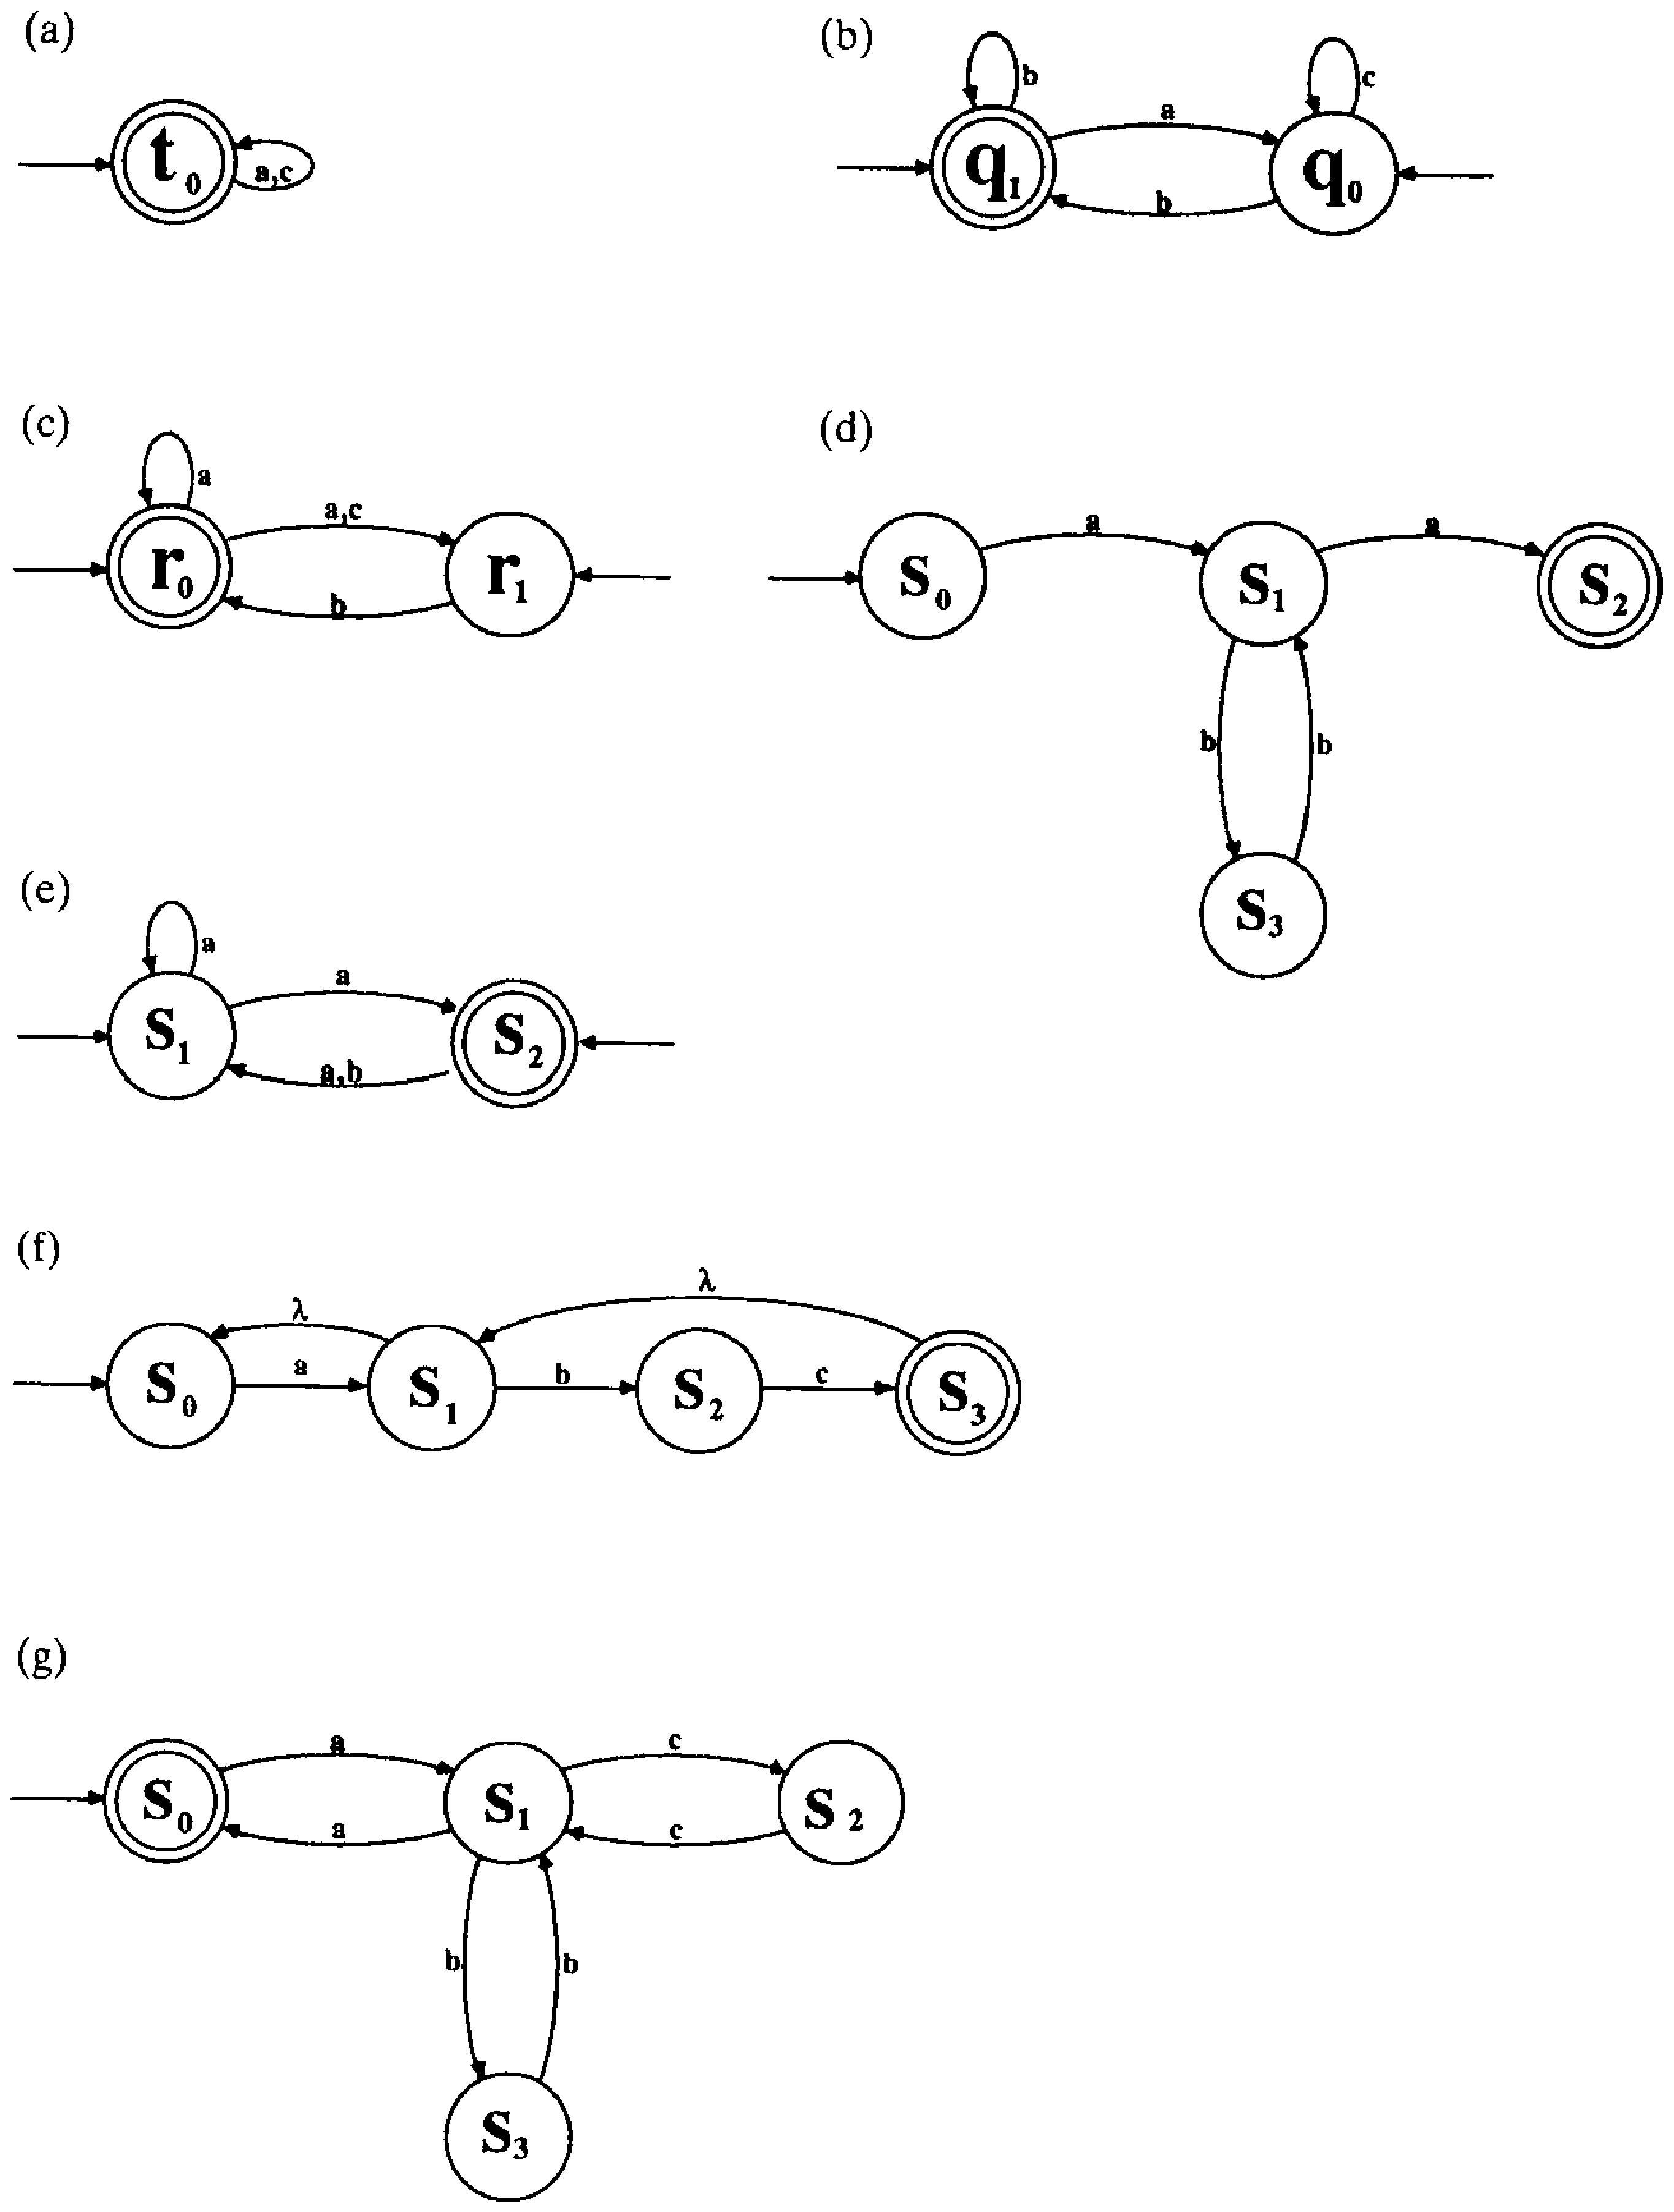
\epsfig{figure=ToFAfigures/fig4-25.eps,width=6.0in}}
\caption{Automata for Exercise 4.1}\label{fig-4.25}
\end{figure}

\item Consider the automaton given in Example 4.4.
\begin{enumerate}
\item Using the standard encodings, draw a circuit diagram for this NDFA
(include neither \<SOS\> nor \<EOS\>)
\item Using the standard encodings, draw a circuit diagram for this NDFA
(include both \<SOS\> and \<EOS\>)
\item Convert the NDFA into a DFA using Definition \ref{dfn-4.5} (draw only the connected
portion of the machine).
\item Convert the NDFA into a DFA using Definition \ref{dfn-4.5} (draw the entire machine,
including the disconnected portion).
\end{enumerate}

\item Consider the automaton given in Example 4.2.
\begin{enumerate}
\item Using the standard encodings, draw a circuit diagram for this NDFA
(include both \<SOS\> and \<EOS\>)
\item Convert the NDFA into a DFA using Definition \ref{dfn-4.5}.
\end{enumerate}

\item Consider the automaton given in Example 4.3.
\begin{enumerate}
\item Using the standard encodings, draw a circuit diagram for this NDFA
(include neither \<SOS\> nor \<EOS\>).
\item Using the standard encodings, draw a circuit diagram for this NDFA
(include both \<SOS\> and \<EOS\>)
\item Convert the NDFA into a DFA using Definition \ref{dfn-4.5} (draw only the connected
portion of the machine).
\item Is this DFA isomorphic to any of the automata constructed in Exercise 4.4?
\end{enumerate}

\item Consider the automaton given in Example 4.14.
\begin{enumerate}
\item Using the standard encodings, draw a circuit diagram for this NDFA
(include neither \<SOS\> nor \<EOS\>)
\item Using the standard encodings, draw a circuit diagram for the NDFA in part
(b) (include neither \<SOS\> nor \<EOS\>)
\end{enumerate}

\item Consider the automaton given in the second part of Example 4.16.
\begin{enumerate}
\item Using the standard encodings, draw a circuit diagram for this NDFA
(include \<EOS\> but not \<SOS\>)
\item Build the equivalent automaton \emph{without} $\lambda$-transitions using
Definition \ref{dfn-4.9}.
\item Using the standard encodings, draw a circuit diagram for the NDFA in part
(b) (include \<EOS\> but not \<SOS\>)
\item Convert the NDFA into a DFA using Definition \ref{dfn-4.5} (draw only the connected
portion of the machine).
\end{enumerate}

\item It is possible to build a \emph{deterministic finite automaton}
$\overline{A}$ such that the language accepted by this machine is the
\emph{absolute complement} of the language accepted by a machine $A$ [that is,
$L(\overline{A})=\Sigma^* - L(A)$] by simply complementing the set of final
states (see Theorem \ref{thm-5.1}). Can a similar thing be done for nondeterministic
finite automata? If not, why not? Give an example to support your statements.

\item Given a nondeterministic finite automaton $A$ \emph{without}
$\lambda$-transitions, show that it is possible to construct a nondeterministic
finite automaton \emph{with} $\lambda$-transitions $A'$ with the properties
\begin{enumerate}[(1)]
\item $A'$ has exactly \emph{one} start state and exactly \emph{one} final state
and
\item $L(A') = L(A)$.
\end{enumerate}

\item Consider (ii) in Definition \ref{dfn-4.8}. Can this fact be deduced from parts (i)
and (iii)? Justify your answer.

\item If we wanted another way to construct a nondeterministic finite automaton
\emph{without} $\lambda$-transitions corresponding to one that does have them,
we could try the following: Let $S'=S,\ S'_0=\Lambda(S_0),\ F'=F$, and
$\delta'(s,\pmb{a})=\DBAR_{\lambda}(s,\pmb{a})$ for all $\pmb{a}\in\Sigma,s \in
S$. Show that this works (or if it does not work, explain why not and give an
example).

\item Using nondeterministic machines \emph{with} $\lambda$-transitions, give an
algorithm for constructing a $\lambda$-NDFA having \emph{one} start state and
\emph{one} final state that will accept the \emph{union} of two FAD languages.

\item Give an example of an NDFA $A$ for which:
\begin{enumerate}
\item $A^d$ is not connected.
\item $A^d$ is not reduced.
\item $A^d$ is minimal.
\end{enumerate}

\item Why was it necessary to include an ``extra'' state $q_0$ in the
construction of $A^{\sigma}_{\lambda}$ in Definition \ref{dfn-4.9}? Support your answer
with an example.

\item \begin{enumerate}
\item Using nondeterministic machines \emph{without} $\lambda$-transitions, give
an algorithm for constructing a machine that will accept the \emph{union} of two
languages.
\item Is this easier or more difficult than using machines \emph{with}
$\lambda$-transitions?
\item Is it possible to ensure that this machine \emph{both} (i) has exactly
\emph{one} start state \emph{and} (ii) has exactly \emph{one} final state?
\end{enumerate}

\item Consider the automaton $A^{\sigma}_{\lambda}$ given in Example 4.15.
\begin{enumerate}
\item Using the standard encodings, draw a circuit diagram for
$A^{\sigma}_{\lambda}$ (include neither \<SOS\> nor \<EOS\>)
\item Convert $A^{\sigma}_{\lambda}$ into $A^{\sigma d}_{\lambda}$ using
Definition \ref{dfn-4.5} (draw only the connected portion of the machine).
\end{enumerate}

\item \begin{enumerate}
\item Prove that for any NDFA \emph{without} $\lambda$-transitions the
definitions of \DBAR\ and $\delta$ agree for single letters; that is,
$(\forall s \in S)(\forall\pmb{a}\in\Sigma)(\DBAR(s,\pmb{a})=\delta(s,\pmb{a}))$.
\item Give an example to show that this need not be true for an NDFA \emph{with}
$\lambda$-transitions.
\end{enumerate}

\item Consider the NDFA that accepts the original language $L$ in Example 4.10.
\begin{enumerate}
\item Using the standard encodings, draw a circuit diagram for this NDFA
(include neither \<SOS\> nor \<EOS\>)
\item Convert the NDFA into a DFA using Definition \ref{dfn-4.5} (draw only the connected
portion of the machine).
\end{enumerate}

\item Consider the NDFA which accepts the modified language $L^r$ in Example
4.10.
\begin{enumerate}
\item Using the standard encodings, draw a circuit diagram for this NDFA
(include neither \<SOS\> nor \<EOS\>)
\item Convert the NDFA into a DFA using Definition \ref{dfn-4.5} (draw only the connected
portion of the machine).
\end{enumerate}

\item Consider the arguments leading up to the pumping lemma in Chapter \ref{ch-2}. Are
they still valid when applied to NDFAs?

\item Consider Theorem \ref{thm-2.7}. Does the conclusion still hold if applied to an
NDFA?

\item Given a nondeterministic finite automaton $A$ (without
$\lambda$-transitions) for which $\lambda \notin L(A)$, show that it is possible
to construct a nondeterministic finite automaton (also without
$\lambda$-transitions) $A''$ with the properties:
\begin{enumerate}[1.]
\item $A''$ has exactly \emph{one} start state.
\item $A''$ has exactly \emph{one} final state.
\item $L(A'') = L(A)$.
\end{enumerate}

\item Give an example to show that if $\lambda \in L(A)$ it may not be possible
to construct an NDFA without $\lambda$-transitions satisfying all three
properties listed in Exercise 4.22.

\item Prove Lemma \ref{lmm-4.2}.

\item Given a DFA $A$, show that it can be thought of as an NDFA $A^n$ and that,
furthermore, $L(A^n) = L(A)$. \emph{Hint:} Carefully define your ``new'' machine
$A^n$, justify that it is indeed an NDFA, make the appropriate inductive
statement, and argue that $L(A^n) = L(A)$.

\item Give an example to show that the domain of Lemma \ref{lmm-4.2} cannot be expanded
to include $\lambda$; that is, show that $\overline{\delta^{\sigma}_{\lambda}}(s,\lambda)
\not= \DBAR_{\lambda}(s,\lambda)$.

\item Refer to Definition \ref{dfn-4.5} and prove the fact used in Lemma \ref{lmm-4.1}:
\[ (\forall A \in \wp(S))(\forall B \in \wp(S))(\forall\pmb{a}\in\Sigma)(\delta^d
	(A \cup B,\pmb{a}) = \delta^d(A,\pmb{a}) \cup \delta^d(B,\pmb{a})) \]
	
\item Recall that if a word can reach several states in an NDFA, some of which
are final and some nonfinal, Definition \ref{dfn-4.4} requires us to accept that word.
\begin{enumerate}
\item Change the definition of $L(A)$ so that a word is accepted only if
\emph{every} state the word can reach is final.
\item Change the definition of $A^d$ to produce a deterministic machine that
accepts only those words specified in part (a).
\end{enumerate}

\item Draw the connected part of $T^d$,the deterministic equivalent of the NDFA
$T$ in Example 4.7.

\item Refer to Example 4.7 and modify the NDFA $T$ so that the machine reverts
to a nonfinal state (that is, turns the recorder off) when the substring
$\pmb{000111}$ is detected. Note that $\pmb{000111}$ functions as the EOT (end
of transmission) signal.

\item Consider the automaton $A$ given in Example 4.14.
\begin{enumerate}
\item Draw a diagram of $A^{\sigma}_{\lambda}$.
\item Draw $A^{\sigma d}_{\lambda}$ (draw only the connected portion of the
machine).
\end{enumerate}

\item What is wrong with the following ``proof'' of Lemma \ref{lmm-4.2}? Let $P(k)$ be
defined by $P(k): (\forall s \in S)(\forall x \in \Sigma^k)
(\overline{\delta^{\sigma}_{\lambda}}(s,x)=\DBAR_{\lambda}(s,x))$. \\
\emph{Basis step} $(k = 1): (\forall s \in S)(\forall\pmb{a}\in\Sigma)
(\overline{\delta^{\sigma}_{\lambda}}(s,\pmb{a})=\delta^{\sigma}_{\lambda}(s,\pmb{a}) =
\DBAR_{\lambda}(s,\pmb{a}))$. \\
\emph{Inductive step}: Suppose that the result holds for all $x \in \Sigma^k$
and let $y \in \Sigma^{k+1}$. Then $(\exists x \in \Sigma^k)(\exists \pmb{a} \in
\Sigma \ni y = x\pmb{a})$. Then
\begin{center}\begin{tabular}{rcl}
$\overline{\delta^{\sigma}_{\lambda}}(s,y)$ & $=$ & $\overline{\delta^{\sigma}_{\lambda}}(s,x\pmb{a})$\\
& $=$ & $\delta^{\sigma}_{\lambda}(\overline{\delta^{\sigma}_{\lambda}}(s,x),\pmb{a})$ \\
& $=$ & $\overline{\delta^{\sigma}_{\lambda}}(\DBAR_{\lambda}(s,x),\pmb{a})$ \\
& $=$ & $\DBAR_{\lambda}(\DBAR_{\lambda}(s,x),\pmb{a})$ \\
& $=$ & $\DBAR_{\lambda}(s,x\pmb{a})$ \\
& $=$ & $\DBAR_{\lambda}(s,y)$
\end{tabular}\end{center}
Therefore, $P(k) \Rightarrow P(k + 1)$ for all $k \geq 1$, and by the principle
of mathematical induction, we are assured that the equation holds for all
$x \in \Sigma^+$.

\item Consider the automaton given in Example 4.7.
\begin{enumerate}
\item Using the standard encodings, draw a circuit diagram for this NDFA
(include neither \<SOS\> nor \<EOS\>)
\item Convert the NDFA into a DFA using Definition \ref{dfn-4.5} (draw only the connected
portion of the machine).
\end{enumerate}

\item Consider the automaton given in Example 4.11.
\begin{enumerate}
\item Using the standard encodings, draw a circuit diagram for this NDFA
(include neither \<SOS\> nor \<EOS\>)
\item Convert the NDFA into a DFA using Definition \ref{dfn-4.5} (draw only the connected
portion of the machine).
\end{enumerate}

\item Consider the automaton B given in Example 4.8.
\begin{enumerate}
\item Using the standard encodings, draw a circuit diagram for $B$ (include
neither \<SOS\> nor \<EOS\>).
\item Using the standard encodings, draw a circuit diagram for $B^d$ (include
neither \<SOS\> nor \<EOS\>). Encode the states in such a way that your circuit is similar
to the one found in part (a).
\end{enumerate}

\item Draw a circuit diagram for each NDFA given in Figure \ref{fig-4.25} (include
neither \<SOS\> nor \<EOS\>). Use the standard encodings.

\item Draw a circuit diagram for each NDFA given in Figure \ref{fig-4.25} (include both
\<SOS\> and \<EOS\>). Use the standard encodings.
(See Example 4.13 for the solution corresponding to Figure \ref{fig-4.25}e.)


\item Definition \ref{dfn-3.10} and the associated algorithms were used in Chapter \ref{ch-3} for
finding the connected portion of a DFA.
\begin{enumerate}
\item Adapt Definition \ref{dfn-3.10} so that it applies to NDFAs.
\item Prove that there is an algorithm for finding the connected portion of an
NDFA.
\end{enumerate}
\end{enumerate}

% Chapter, Section, Figure, Table, Theorem, Corollary, Lemma, Definition, {\bf  
\chapter{Closure Properties}\label{ch-5}

In this chapter we will look at ways to combine languages that are recognized
by finite automata (that is, FAD languages) and consider whether the
combinations result in other FAD languages. These results will provide insights
into the construction of finite automata and will establish useful information
that will have bearing on the topics covered in later chapters. After the
properties of the collection of FAD languages have been fully explored, other
classes of languages will be investigated. \\
We begin with a review of the concept of \emph{\Index{closure}}.

\section{FAD Languages and Basic Closure Theorems}\label{sec-5.1}

Notice that when many everyday operators combine objects of a given type they
produce an object of the same type. In arithmetic, for example, the
multiplication of any two whole numbers produces another whole number. Recall
that this property is described by saying that the set of whole numbers is
\emph{closed}\index{closed|see{closure}} under the operation of multiplication. In contrast, the
quotient of two whole numbers is likely to produce a fraction: the whole numbers
are not closed under division. The formal definition of closure, both for
operators that combine two other objects (binary operators) and those that
modify only one object (unary operators) is given below.

% Definition 5.1
\begin{dfn}\label{dfn-5.1}
The \emph{set $K$ is closed under the (binary) operator $\THETA$} iff
$(\forall x,y \in K)(x\THETA y \in K)$.
\end{dfn}

% Definition 5.2
\begin{dfn}\label{dfn-5.2}
The \emph{set $K$ is closed under the (unary) operator $\ETA$} iff
$(\forall x \in K)(\ETA(x) \in K)$.
\end{dfn}

\subsection*{Example 5.1}

$\NN$ is closed under $+$ since, if $x$ and $y$ are nonnegative integers, then
$x + y$ is another nonnegative integer; that is, if $x,y \in \NN$, then
$x + y \in \NN$.

\subsection*{Example 5.2}

$\ZN$ is closed under $|\ |$ (absolute value), since if $x$ is an integer, $|x|$
is also an integer.

\subsection*{Example 5.3}

%jc perhaps we don't want emph below...
Let $\rho =\{X$ $|$ X is a \emph{finite} subset of $\NN\}$; then $\rho$ is closed under
$\cup$, since the union of two finite sets is still finite. (If $Y$ and $Z$ are
subsets for which $\|Y\| = n < \infty$ and $\|Z\| = m < \infty$, then
$\|Y \cup Z\| \leq n + m < \infty$. Under what conditions would
$\|Y \cup Z\| < n + m$?)

To show a set $K$ is not closed under a binary operator $\THETA$, we must show
$\neg[(\forall x,y \in K)(x\THETA y \in K)]$, which means
$\exists x,y \in K \ni x\THETA y \notin K$.

\subsection*{Example 5.4}

$\NN$ is not closed under $-$ (subtraction) since $3 - 5 = -2 \notin \NN$, even
though both $3 \in \NN$ and $5 \in \NN$.

Notice that the set as well as the operator is important when discussing closure
properties; unlike $\NN$, the set of all integers $\ZN$ is closed under
subtraction. As with the binary operator in Example 5.4, a single counterexample
is sufficient to show that a given set is not closed under a unary operator.

\subsection*{Example 5.5}

%jc Shenanigans to get an overbar without the symbol sinking far below the line.
$\NN$ is not closed under $\sqrt{\huge \ ^{\ ^{\ }}}$ (square root) since $7 \in \NN$ but
$\sqrt{7} \notin \NN$.

We will not be concerned so much with sets of numbers as with sets of languages.
As in Example 5.3, the collection will be a set of sets. Of prime concern are
those languages that are related to automata.

% Definition 5.3
\begin{dfn}\label{dfn-5.3}\index{D@\DSIG \ (D-sigma )}
Let $\Sigma$ be an alphabet. The symbol \DSIG\, is used to denote the
set of all FAD languages over $\Sigma$; that is,
$$ \DSIG =\{L \subseteq \Sigma^*\ |\ \exists
\text{ deterministic finite automaton } M \ni L(M) = L\} $$
\end{dfn}

\DSIG\ is the set of all languages that can be recognized by
finite automata. In this chapter, it is this set whose closure properties with
respect to various operations in $\Sigma^*$ we are most interested in
investigating. For example, if there exists a machine that accepts a language
$K$, then there is also a machine that accepts the complement of $K$. That is,
if $K$ is FAD, then $\sim\!\! K$ is FAD: $\DSIG$ is closed under
$\sim$.

% Theorem 5.1
\begin{thm}\label{thm-5.1}\index{closure!under complementation}
For any alphabet $\Sigma$, $\DSIG$ is closed under $\sim$
(complementation).

\emph{Proof.} Let $K \in \DSIG$. We must show $\sim\!\! K \in
\DSIG$ also; that is, there is a machine that recognizes
$\sim\!\! K$. But $K \in \DSIG$, and thus there is a deterministic
finite automaton that recognizes $K$: Let
$A =\langle\Sigma,S,s_0,\delta,F\rangle$ and $L(A) = K$. Define a new machine
$A^\sim$ as follows:
$A^\sim =\langle\Sigma,S^\sim,s_0^\sim,\delta^\sim,F^\sim\rangle =
\langle\Sigma,S,s_0,\delta,S$-$F\rangle$, which looks just like $A$ except that
the final and nonfinal states have been interchanged. We claim that
$L(A^\sim) =\ \sim\!\! K$. To show this, let $x$ be an arbitrary element of
$\Sigma^*$. Then
\begin{center}
\begin{tabular}{rcl}
$x \in L(A^\sim)$ & $\Leftrightarrow$ & (by definition of $L$) \\
$\overline{\delta^\sim}(s_0^\sim,x) \in F^\sim$ & $\Leftrightarrow$ &
	(by induction and the fact that $\delta = \delta^\sim$) \\
$\DBAR(s_0^\sim,x) \in F^\sim$ & $\Leftrightarrow$ &
	(by definition of $s_0^\sim$) \\
$\DBAR(s_0,x) \in F^\sim$ & $\Leftrightarrow$ &
	(by definition of $F^\sim$) \\
$\DBAR(s_0,x)\in S$-$F$ & $\Leftrightarrow$ &
	(by definition of complement) \\
$\DBAR(s_0,x) \notin F$ & $\Leftrightarrow$ &
	(by definition of $L$) \\
$x \notin L(A)$ & $\Leftrightarrow$ &
	(by definition of $K$) \\
$x \notin K$ & $\Leftrightarrow$ &
	(by definition of complement) \\
$x \in\ \sim\!\! K$ &&
\end{tabular}
\end{center}
Thus $L(A^\sim) =\ \sim\!\! K$ as claimed, and therefore the complement of any FAD
language can also be recognized by a machine and is consequently also FAD. Thus
$\DSIG$ is closed under complementation.
\end{thm}

It turns out that $\DSIG$ is closed under all the common set
operators. Notice that the definition of $\DSIG$ implies that we
are working with only one alphabet; if we combine two machines in some way, it
is understood that both automata use exactly the same input alphabet. This turns
out to be not much of a restriction, however, for if we wish to consider two
machines that use different alphabets $\Sigma_1$ and $\Sigma_2$, we can simply
modify each machine so that it is able to process the new common alphabet
$\Sigma = \Sigma_1 \cup \Sigma_2$. It should be clear that this can be done in
such a way as not to affect the language accepted by either machine (see the
exercises).

We will now prove that the union of two FAD languages is also FAD. This can be
shown by demonstrating that, given two automata $M_1$ and $M_2$, it is possible
to construct another automaton that recognizes the union of the languages
accepted by $M_1$ and $M_2$.

\subsection*{Example 5.6}

Consider the two machines $M_1$ and $M_2$ displayed in Figure \ref{fig-5.1}. These two
machines can easily be employed to construct a \emph{non}deterministic finite automaton
that clearly accepts the appropriate union. We simply need to combine them into
a single machine, which in this case will have two start states, as shown in
Figure \ref{fig-5.2}.

The structure inside the dotted box should be viewed as a single \underline NDFA with two
start states. Any string that would be accepted by $M_1$ will reach a final
state if it starts in the ``upper half'' of the new machine, while strings that
are recognized by $M_2$ will be accepted by the ``lower half'' of the machine.
Recall that the definition of acceptance by a nondeterministic finite automaton
implies that the NDFA in Figure \ref{fig-5.2} will accept a string if \emph{any} path leads to a
final state. This new NDFA will therefore accept all the strings that $M_1$
accepted and all the strings that $M_2$ accepted. Furthermore, these are the
\emph{only} strings that will be accepted. This trick is the basis of the following
proof, which demonstrates the convenience of using the NDFA concept; a proof
involving only DFAs would be both longer and less obvious (see the exercises).

% Figure 5.1
\begin{figure}
\centerline{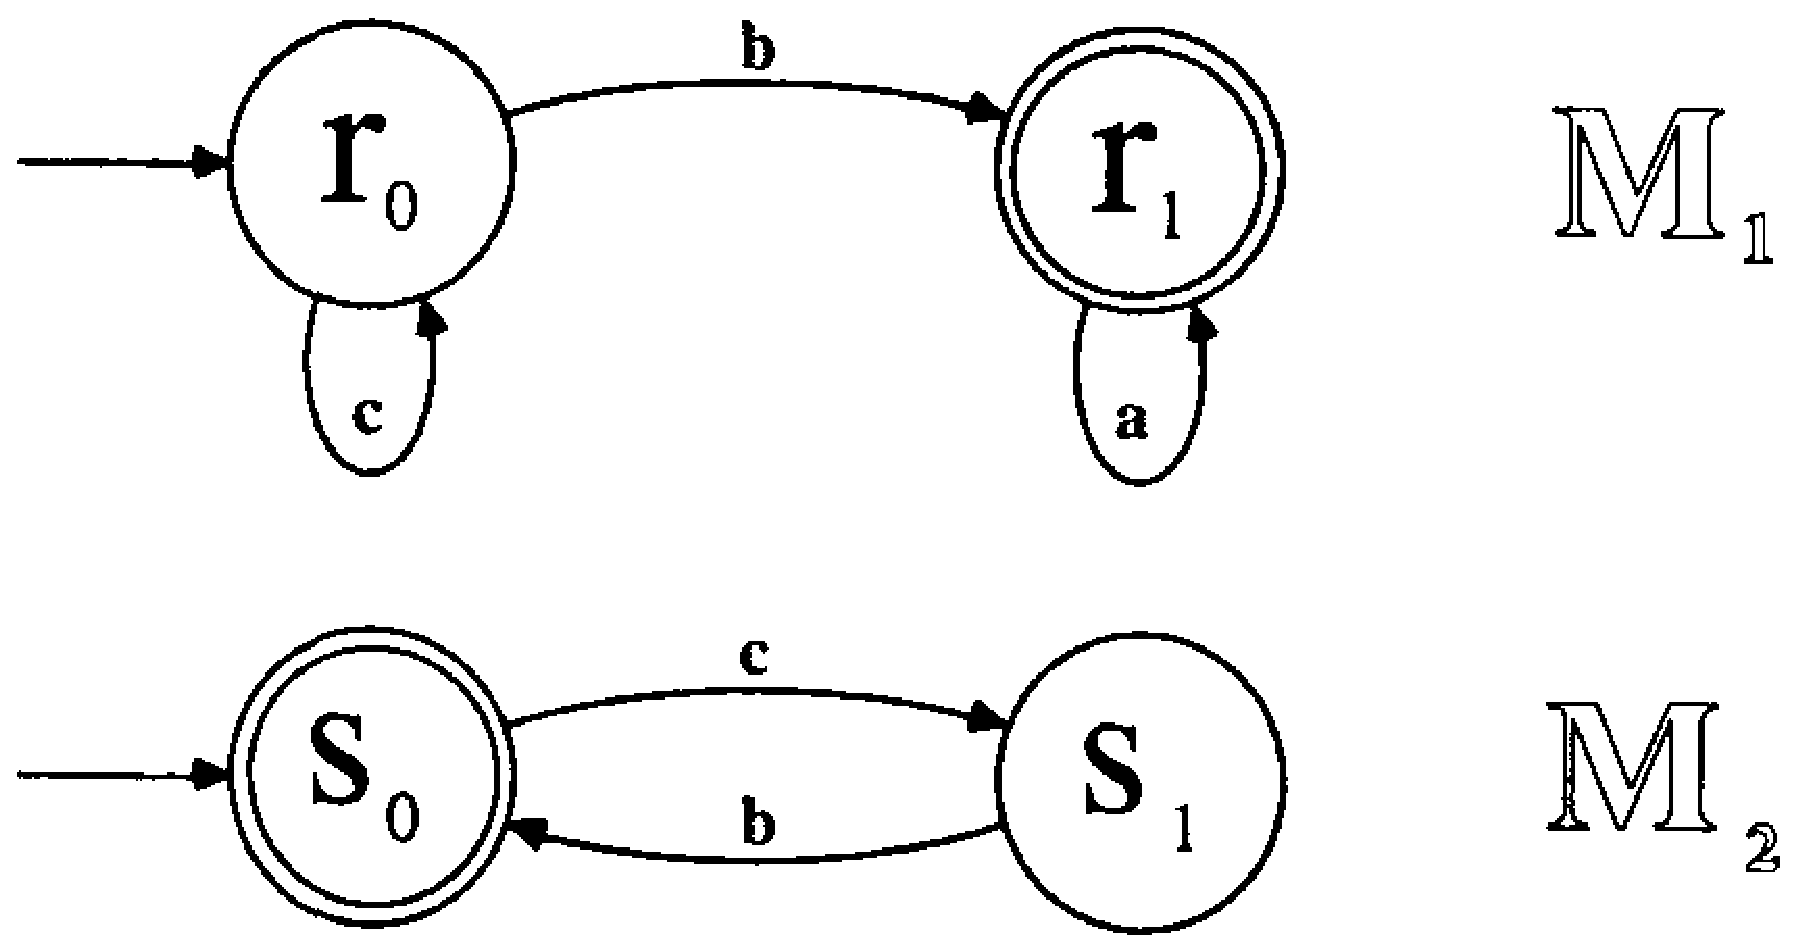
\epsfig{figure=ToFAfigures/fig5-1.eps,width=3in}}
\caption{The two automata discussed in Example 5.6}\label{fig-5.1}
\end{figure}

% Figure 5.2
\begin{figure}
\centerline{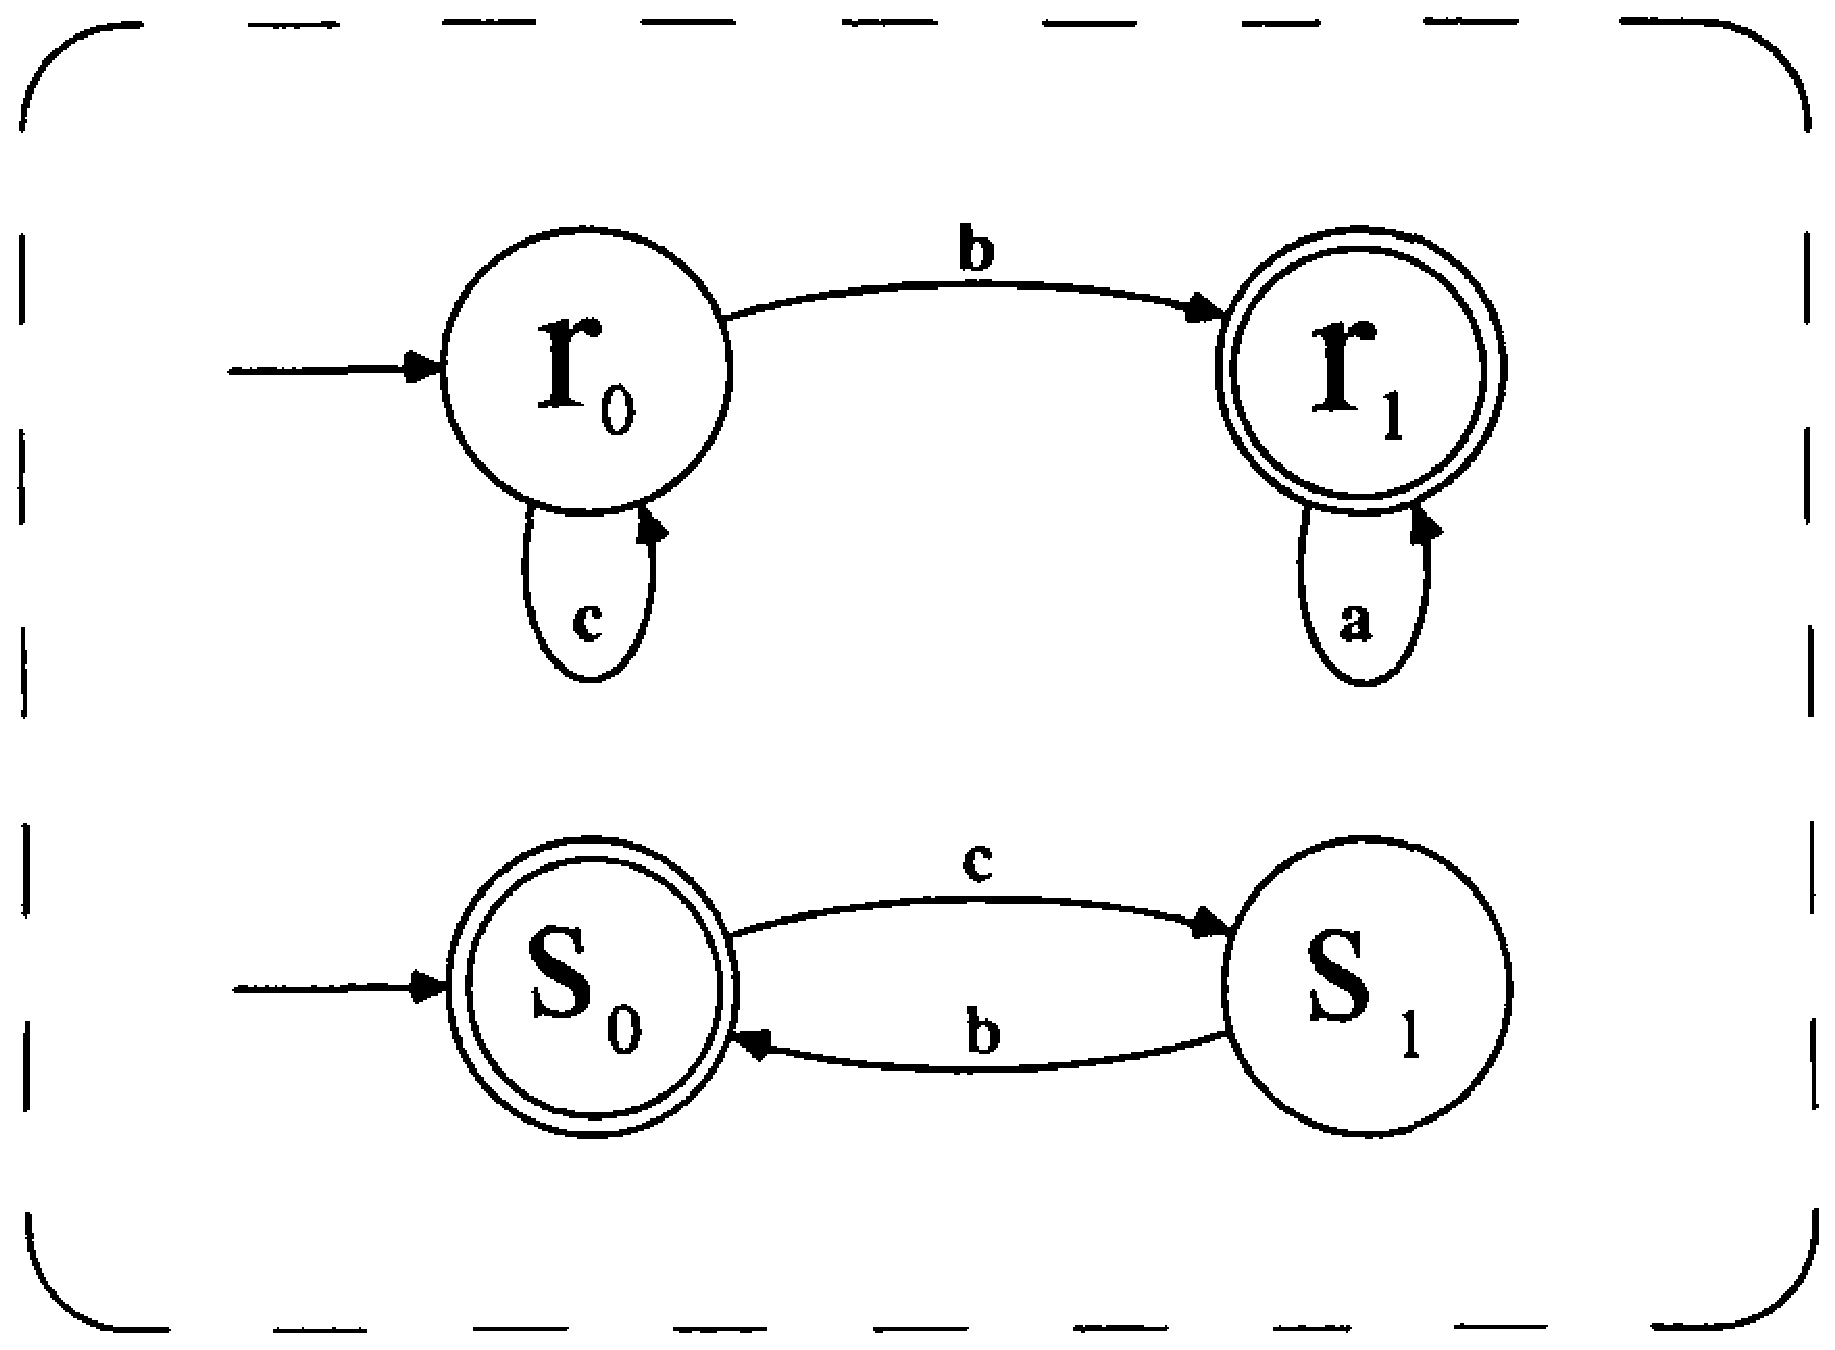
\epsfig{figure=ToFAfigures/fig5-2.eps,width=3in}}
\caption{The resulting automaton in Example 5.6}\label{fig-5.2}
\end{figure}

% Theorem 5.2
\begin{thm}\label{thm-5.2}\index{closure!under union}
For any alphabet $\Sigma$, $\DSIG$ is closed under $\cup$.

\emph{Proof.} Let $L_1$ and $L_2$ belong to $\DSIG$. Then there
are \underline{non}deterministic finite automata
$A_1 =\langle\Sigma,S_1,S_{0_1},\delta_1,F_1\rangle$ and
$A_2 =\langle\Sigma,S_2,S_{0_2},\delta_2,F_2\rangle$ such that $L(A_1)=L_1$ and
$L(A_2)=L_2$ (why?). Define
$A^\cup =\langle\Sigma,S^\cup,S_0^\cup,\delta^\cup,F^\cup\rangle$, where
\begin{center}
\begin{tabular}{ll}
$S^\cup = S_1 \cup S_2$ & (without loss of generality, we can assume
	$S_1 \cap S_2 = \emptyset$) \\
$S_0^\cup = S_{0_1} \cup S_{0_2}$ & \\
$F^\cup = F_1 \cup F_2$ &
\end{tabular}
\end{center}
and $\delta^\cup$$:\ (S_1 \cup S_2) \times \Sigma \rightarrow \wp(S_1 \cup S_2)$ is
defined by
\[ \delta^\cup(s,\pmb{a}) = \left\{\begin{array}{lr}
				\delta_1(s,\pmb{a}) & \text{if }s \in S_1 \\
				& , \\
				\delta_2(s,\pmb{a}) & \text{if }s \in S_2
			     \end{array}\right.
\quad \forall s \in S_1 \cup S_2,\quad \forall \pmb{a} \in \Sigma \]
We claim that $L(A^\cup)=L(A_1) \cup L(A_2)=L_1 \cup L_2$. This must be proved
using the definition of $L$ from Chapter \ref{ch-4}, since $A_1,\ A_2$, and $A^\cup$ are
all NDFAs.
\begin{center}
\begin{tabular}{rcl}
$x \in L(A^\cup)$ & $\Leftrightarrow$ & (from Definition \ref{dfn-4.4}) \\
$(\exists s \in S_0^\cup)[\overline{\delta^\cup}(s,x) \cap F^\cup \not= \emptyset]$ &
	$\Leftrightarrow$ & (by definition of $S_0^\cup$) \\
$(\exists s \in S_{0_1} \cup S_{0_2})[\overline{\delta^\cup}(s,x) \cap F^\cup\not=\emptyset]$
	& $\Leftrightarrow$ & (by definition of $\cup$) \\
$(\exists s \in S_{0_1})[\overline{\delta^\cup}(s,x) \cap F^\cup \not= \emptyset] \vee
	(\exists s \in S_{0_2})[\overline{\delta^\cup}(s,x) \cap F^\cup \not= \emptyset]$ & 
	$\Leftrightarrow$ & (by definition of $\delta^\cup$ and induction) \\
$(\exists s \in S_{0_1})[\DBAR_1(s,x) \cap F^\cup \not= \emptyset] \vee
	(\exists s \in S_{0_2})[\DBAR_2(s,x) \cap F^\cup \not= \emptyset]$ &
	$\Leftrightarrow$ & (by definition of $F^\cup$) \\
$(\exists s \in S_{0_1})[\DBAR_1(s,x) \cap F_1 \not= \emptyset] \vee
	(\exists s \in S_{0_2})[\DBAR_2(s,x) \cap F_2 \not= \emptyset]$ &
	$\Leftrightarrow$ & (from Definition \ref{dfn-4.4}) \\
$x \in L(A_1) \vee x \in L(A_2)$ & $\Leftrightarrow$ &
	(by definition of $\cup$) \\
$x \in (L(A_1) \cup L(A_2))$ & $\Leftrightarrow$ & (by definition of $L_1,L_2$)\\
$x \in L_1 \cup L_2$ &&
\end{tabular}
\end{center}
\end{thm}

The above ``proof'' is actually incomplete; the transition from line 4 to line 5
actually depends on the assumed properties of $\overline{\delta^\cup}$, and not the known
properties of $\delta^\cup$. A rigorous justification should include an
inductive proof of (or at least a reference to) the fact that $\overline{\delta^\cup}$
reflects the same sort of behavior that $\delta^\cup$ does; that is,
\[ \overline{\delta^\cup}(s,x) = \left\{\begin{array}{lr}
				\DBAR_1(s,x) & \text{if }s \in S_1 \\
				& , \\
				\DBAR_2(s,x) & \text{if }s \in S_2
			     \end{array}\right.
\quad \forall s \in S_1 \cup S_2,\quad \forall x \in \Sigma^* \]
The above rule essentially states that the definition that applies to the single
letter $\pmb{a}$ also applies to the string $x$, and it is easy to prove by
induction on the length of $x$ (see the exercises).

The following theorem, which states that $\DSIG$ is closed under
$\cap$, will be justified in two separate ways. The first proof will argue that
the closure property must hold due to previous results; no new DFA need be
constructed. The drawback to this type of proof is that we have no suitable
guide for actually combining two existing DFAs into a new machine that will
recognize the appropriate intersection (although, as outlined in the exercises,
in this case a construction based on the first proof is fairly easy to generate).

Some operators are so bizarre that a nonconstructive proof of closure is the
best we can hope for; intersection is definitely \emph{not} that strange,
however. In a second proof of the closure of $\DSIG$ under $\cap$,
Lemma \ref{lmm-5.1} will explicitly outline how an intersection machine could be built.
When such constructions can be demonstrated, we will say that
$\DSIG$ is \emph{effectively} closed under the operator in
question (see Theorem \ref{thm-5.12} for a discussion of an operator that is not
effectively closed).

% Theorem 5.3
\begin{thm}\label{thm-5.3}\index{closure!under intersection}
For any alphabet $\Sigma$, $\DSIG$ is closed under $\cap$.

\emph{Proof.} Let $L_1$ and $L_2$ belong to $\DSIG$. Then by
Theorem \ref{thm-5.1}, $\sim\!\! L_1$ and $\sim\!\! L_2$ are also FAD. By Theorem \ref{thm-5.2},
$\sim\!\! L_1 \cup \sim\!\! L_2$ is also FAD. By Theorem \ref{thm-5.1} again,
$\sim\!\!(\sim\!\! L_1 \cup \sim\!\! L_2)$ is also FAD. By De Morgan's law, this
last expression is equivalent to $L_1 \cap L_2$, so $L_1 \cap L_2$ is FAD, and
thus $L_1 \cap L_2 \in \DSIG$.
\end{thm}

Note that the above argument could be made to apply to \emph{any} collection C
of sets that were known to be closed under union and complementation. A second
proof of Theorem \ref{thm-5.3} might rely on the following lemma, using the ``direct''
method of constructing a deterministic machine that accepts $L_1 \cap L_2$. This
would show that $\DSIG$ is \emph{effectively} closed under the
intersection operator.

% Lemma 5.1
\begin{lmm}\label{lmm-5.1}\index{closure!under intersection}\index{cross product}
Given \emph{deterministic} finite automata
$A_1 =\langle\Sigma,S_1,s_{0_1},\delta_1,F_1\rangle$ and
$A_2 =\langle\Sigma,S_2,s_{0_2},\delta_2,F_2\rangle$ such that $L(A_1)=L_1$, and
$L(A_2) = L_2$, define a new DFA
$A^\cap =\langle\Sigma,S^\cap,s_0^\cap,\delta^\cap,F^\cap\rangle$, where
\begin{center}
\begin{tabular}{l}
$S^\cap = S_1 \times S_2$ \\
$s_0^\cap = \langle s_{0_1},s_{0_2}\rangle$ \\
$F^\cap = F_1 \times F_2$
\end{tabular}
\end{center}
and $\delta^\cap$$:\ (S_1 \times S_2) \times \Sigma \rightarrow S_1 \times S_2$ is
defined by
\[ \delta^\cap(\langle s,t\rangle,\pmb{a}) = \langle\delta_1(s,\pmb{a}),\delta_2(t,\pmb{a})\rangle\quad
	\forall s \in S_1, \forall t \in S_2, \forall \pmb{a} \in \Sigma \]
Then $L(A^\cap) = L_1 \cap L_2.$

\emph{Proof.} As usual, the key is to show that
$x \in L(A^\cap) \Leftrightarrow x \in L_1 \cap L_2$. The proof hinges on the
inductive statement that $\overline{\delta^\cap}$ obeys the same rule that defines
$\delta^\cap$; that is,
$(\forall s \in S_1)(\forall t \in S_2)(\forall x \in \Sigma^*)
[\overline{\delta^\cap}(\langle s,t\rangle,x)=\langle\DBAR_1(s,x),\DBAR_2(t,x)\rangle]$. The details are left for the
reader (see the exercises).
\end{lmm}

% Figure 5.3
\begin{figure}
\centerline{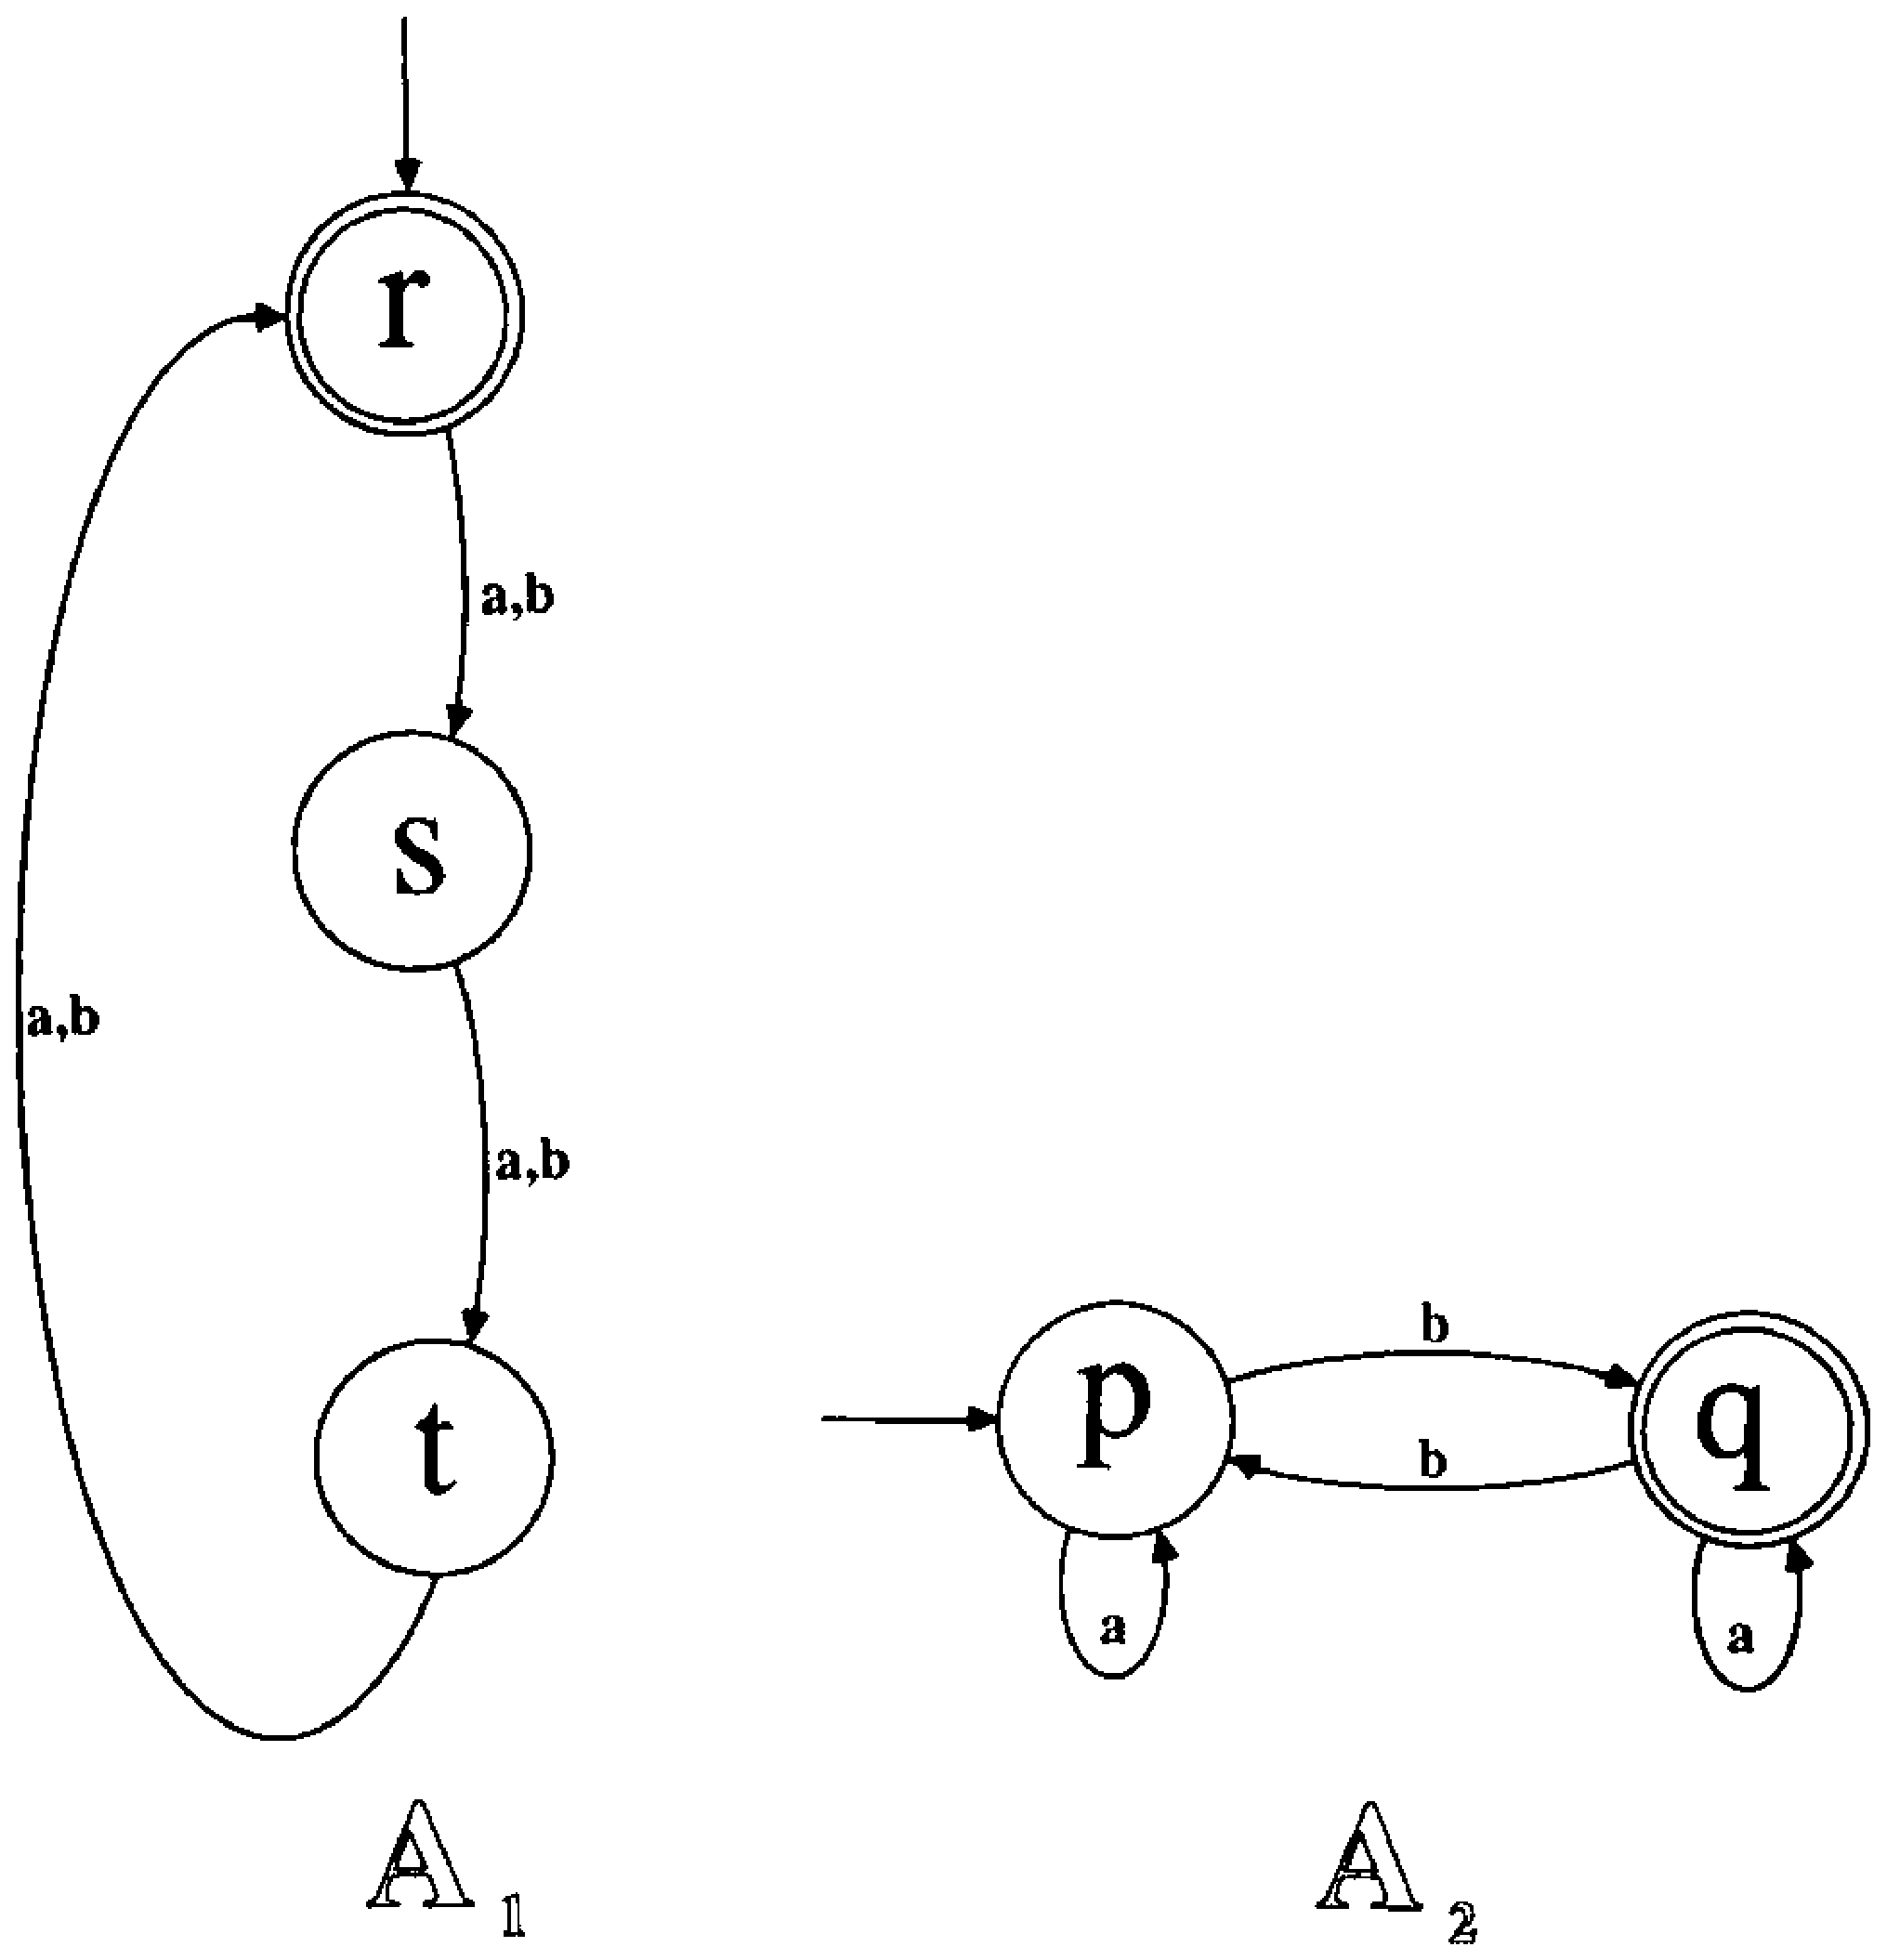
\epsfig{figure=ToFAfigures/fig5-3.eps,height=3.6in}}
\caption{The automata discussed in Example 5.7}\label{fig-5.3}
\end{figure}

The idea behind the above construction is to build a machine that ``remembers''
the state changes that both $A_1$ and $A_2$ make as they each process the same
string, and hence the state set consists of all possible pairs of states from
$A_1$ and $A_2$. The goal was to design the transition function $\delta^\cap$ so
that being in state $\langle s,t\rangle$ in $A^\cap$ indicates that $A_1$ would
currently be in state $s$ and $A_2$ would be in state $t$. This goal also
motivates the definition of the new start state; we want to begin in the start
states of $A_1$ and $A_2$, and hence $s_0^\cap =\langle s_{0_1},s_{0_2}\rangle$.
We only wish to accept strings that are common to both languages, which means
that the terminating state in $A_1$ belongs to $F_1$ and the last state reached
in $A_2$ is likewise a final state. This requirement naturally leads to the
definition of $F^\cap$, where $\langle s,t\rangle$ is a final state if and only
if both $s$ and $t$ were final states in their respective machines.

\subsection*{Example 5.7}

Consider the two machines $A_1$ and $A_2$ displayed in Figure \ref{fig-5.3}. Note that
$A_2$ ``remembers'' whether there have been an even or an odd number of
$\pmb{b}$s, while $A_1$ ``counts'' the number of letters ($\bmod{ 3}$). We now
demonstrate how the definition in Lemma \ref{lmm-5.1} can be applied to form a
deterministic machine that accepts the intersection of $L(A_1)$ and $L(A_2)$.
The structure of $A^\cap$ would in this case look like the automaton shown in
Figure \ref{fig-5.4}. Note that $A^\cap$ does indeed keep track of the criteria that both
$A_1$ and $A_2$ use to accept or reject strings. We will be in a state on the
right side of $A^\cap$ if an odd number of $\pmb{b}$s have been seen and on the
left side when an even number of $\pmb{b}$s have been processed. At the same time,
we will be in the upper, middle, or lower row of states depending on the total
number of letters$\pmod{3}$ that have been processed. There is but one final
state, corresponding to the situation where we have both an odd number of
$\pmb{b}$s and the letter count is $0 \pmod{ 3}$.

% Figure 5.4
\begin{figure}
\centerline{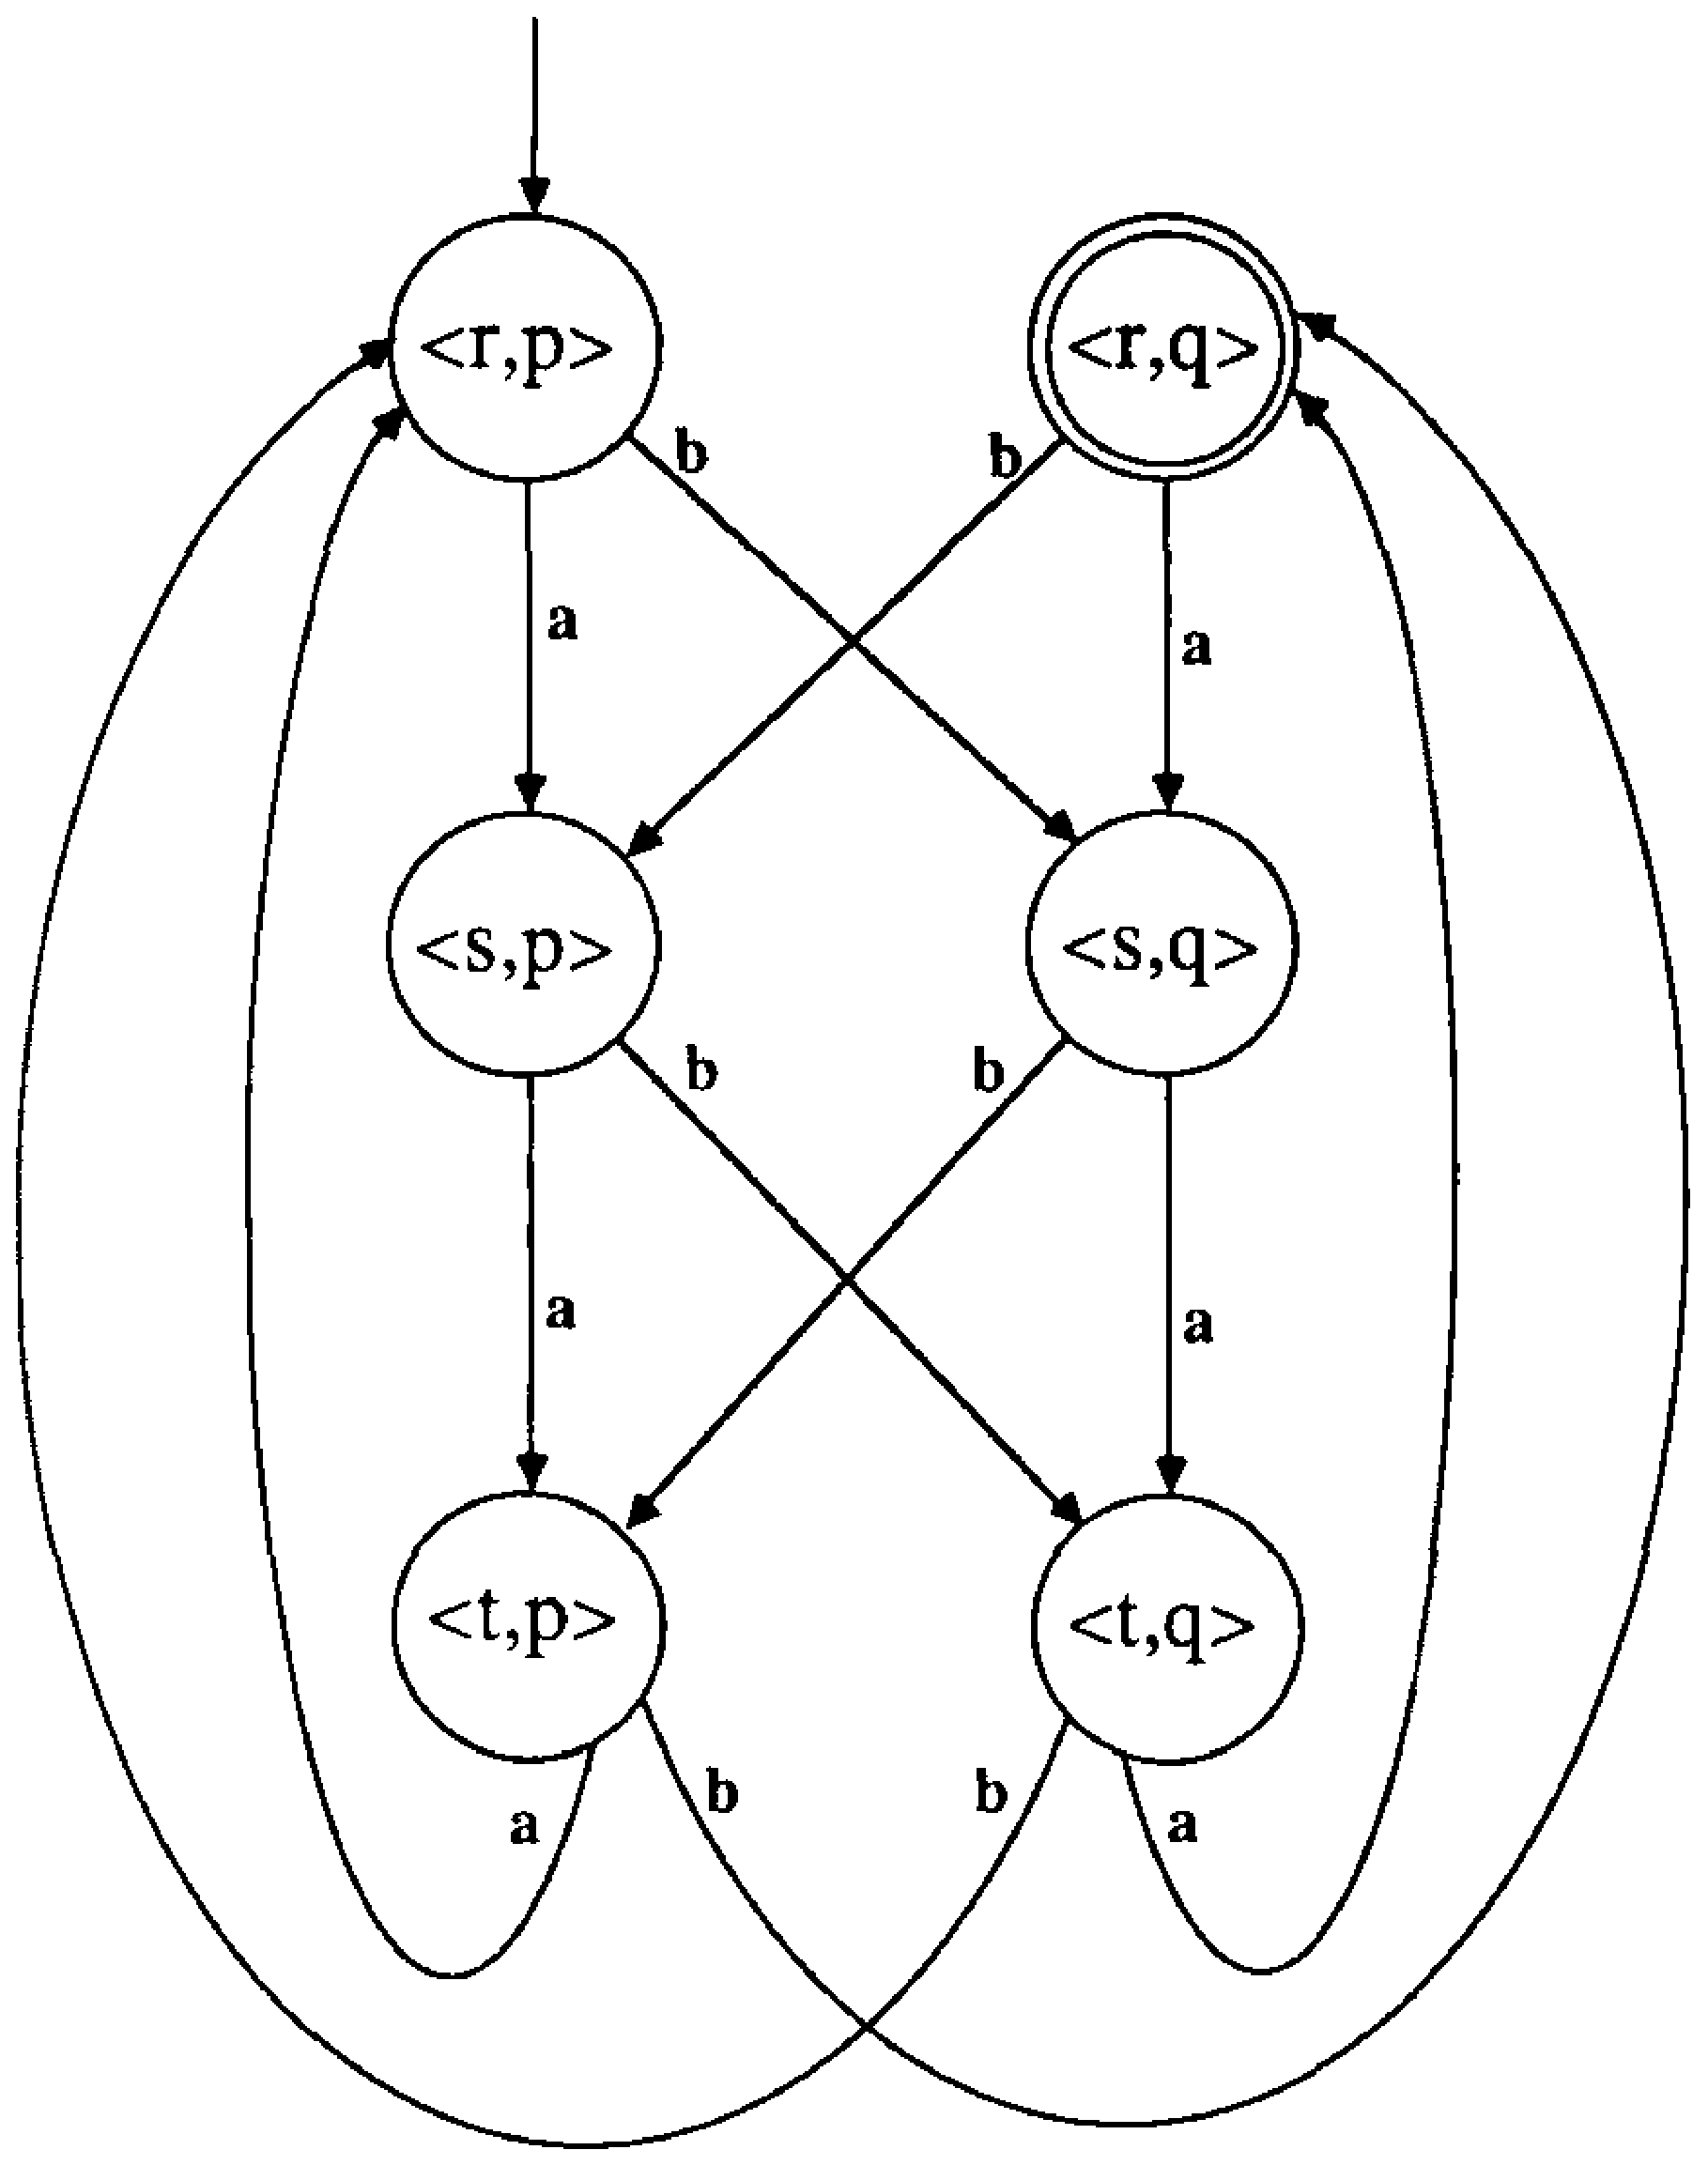
\epsfig{figure=ToFAfigures/fig5-4.eps,height=3.6in}}
\caption{The resulting DFA for Example 5.7}\label{fig-5.4}
\end{figure}

The operations used in the previous three theorems are common to set theory. We
now present some new operators that are special to string algebra. We have
defined concatenation $(\cdot)$ for individual strings, but there is a natural
extension of the definition to languages, as indicated by the next definition.

% Definition 5.4
\begin{dfn}\label{dfn-5.4}\index{concatenation!of languages}
Let $L_1$ and $L_2$ be languages. The \emph{concatenation} of $L_1$ with
$L_2$, written $L_1 \cdot L_2$, is defined by
\[ L_1 \cdot L_2 =\{x\cdot y\ |\ x \in L_1 \wedge y \in L_2\} \]
\end{dfn}

\subsection*{Example 5.8}

If $L_1 =\{\lambda,\pmb{b},\pmb{cc}\}$ and $L_2=\{\lambda,\pmb{aa},\pmb{baa}\}$,
then
\[ L_1 \cdot L_2 =\{\lambda, \pmb{b},\pmb{cc},\pmb{aa},\pmb{baa},\pmb{ccaa},
	\pmb{bbaa},\pmb{ccbaa}\}. \]

Note that $\pmb{baa}$ qualifies to be in $L_1\cdot L_2$ for two reasons:
$\pmb{baa} = \lambda \cdot \pmb{baa}$ and $\pmb{baa} = \pmb{b} \cdot \pmb{aa}$.
Thus we see that the concatenation contains only eight words rather than the
expected $9( = 3\cdot 3)$. In general, $L_1 \cdot L_2$ consists of all words
that can be formed by the concatenation of a word from $L_1$ with a word from
$L_2$; for finite sets, concatenating an $n$ word set with an $m$ word set
results in no more than $n \cdot m$ words. As shown in this example, the number
of words can actually be less than $n \cdot m$. Larger languages can be
concatenated, also. For example, $\Sigma^* \cdot \Sigma = \Sigma^+$.

The concatenation of two FAD languages is also FAD, as can easily be seen by
employing NDFAs with $\lambda$-transitions.

\subsection*{Example 5.9}

Figure \ref{fig-5.5} illustrates two nondeterministic finite automata $B_1$ and $B_2$ that
accept the languages $L_1$ and $L_2$ given in Example 5.8. Combining these two
machines and linking the final states of $B_1$ to the start states of $B_2$ with
$\lambda$-transitions yields a new NDFA that accepts $L_1 \cdot L_2$, as shown
in Figure \ref{fig-5.6}.

% Figure 5.5
\begin{figure}
\centerline{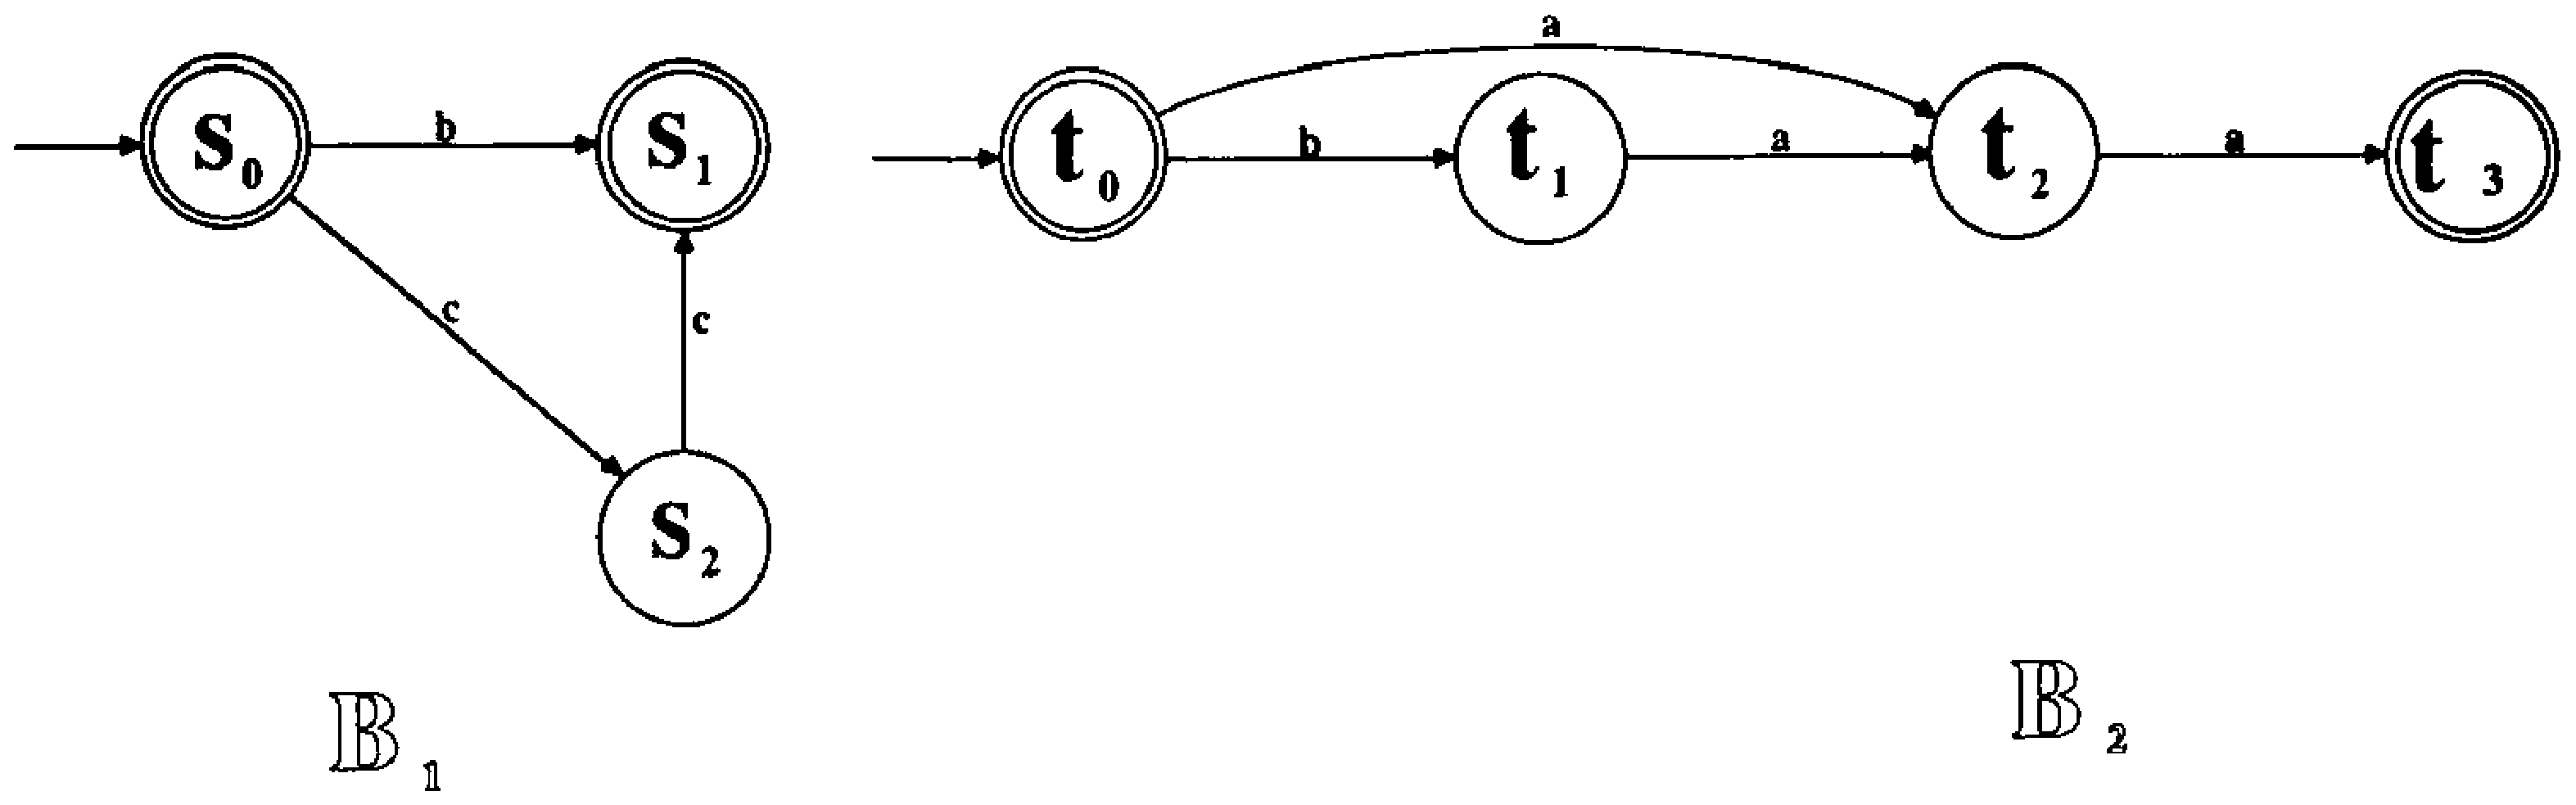
\epsfig{figure=ToFAfigures/fig5-5.eps,width=6in}}
\caption{Two candidates for concatenation}\label{fig-5.5}
\end{figure}

% Figure 5.6
\begin{figure}
\centerline{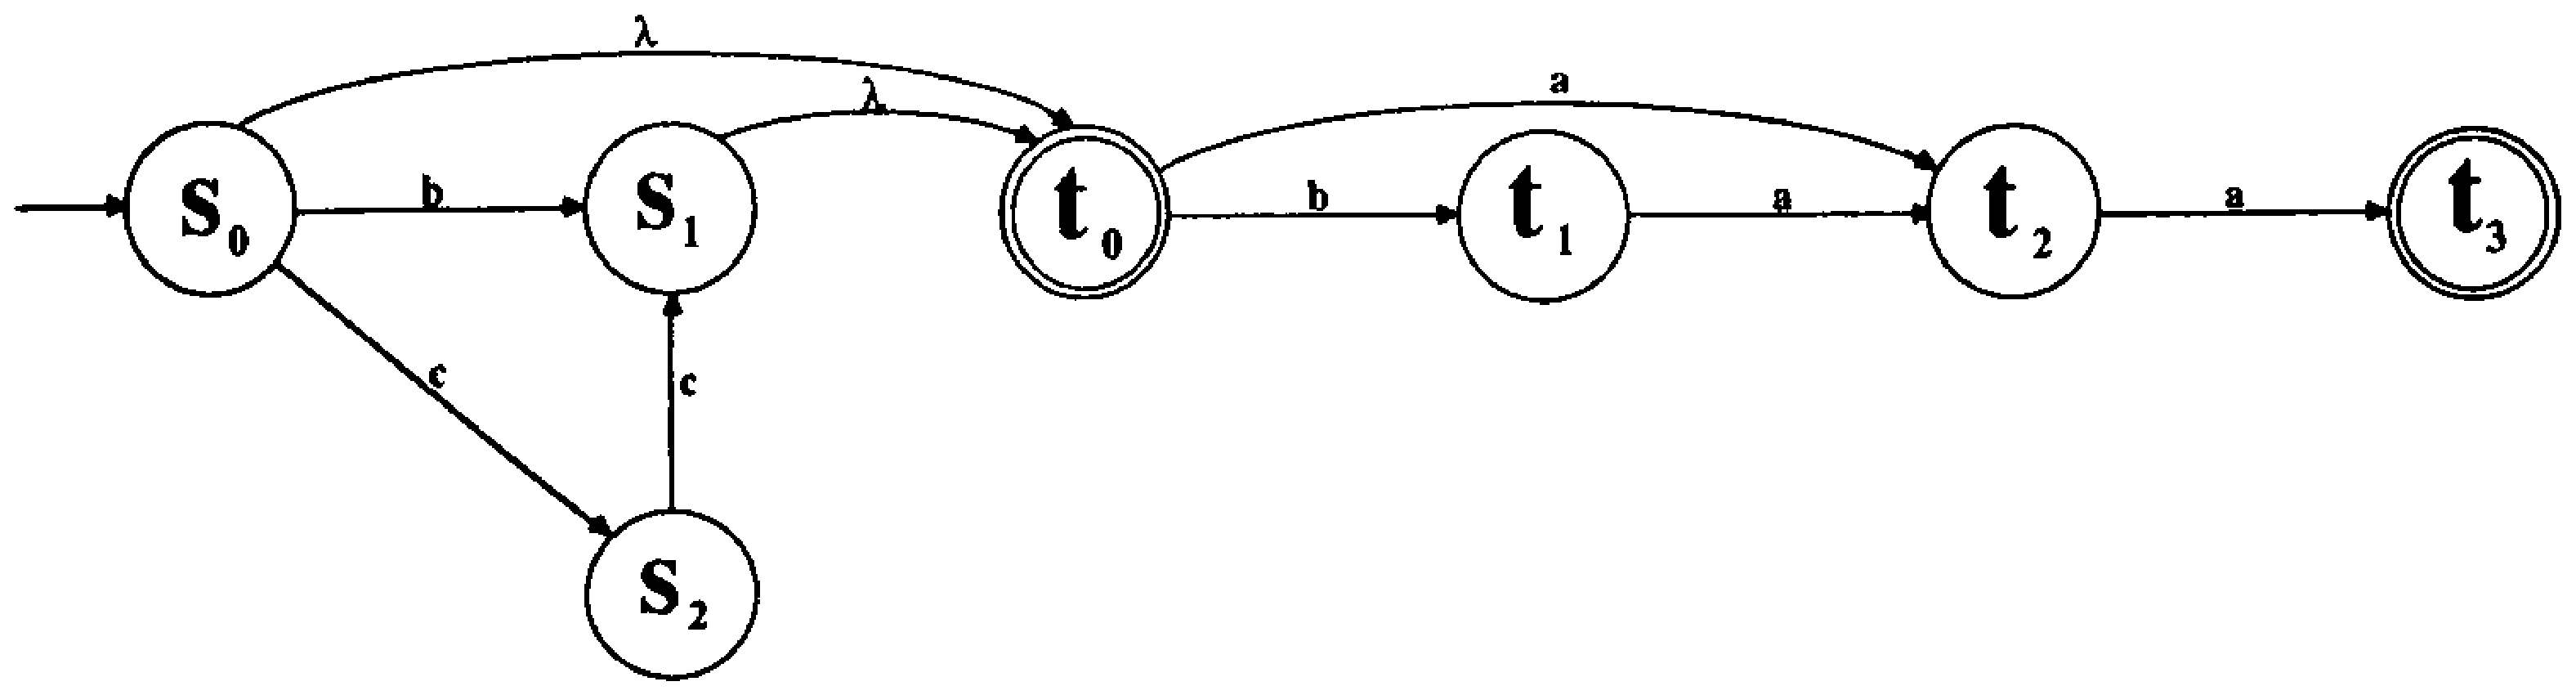
\epsfig{figure=ToFAfigures/fig5-6.eps,width=6in}}
\caption{An NDFA which accepts the concatenation of the machines discussed in
Example 5.9}\label{fig-5.6}
\end{figure}

\subsection*{Example 5.10}

Consider the \emph{deterministic} finite automata $A_1$ and $A_2$ displayed in
Figure \ref{fig-5.7}. These can similarly be linked together to form an NDFA that accepts
the concatenation of the languages accepted by $A_1$ and $A_2$, as shown in
Figure \ref{fig-5.8}.

% Figure 5.7
\begin{figure}
\centerline{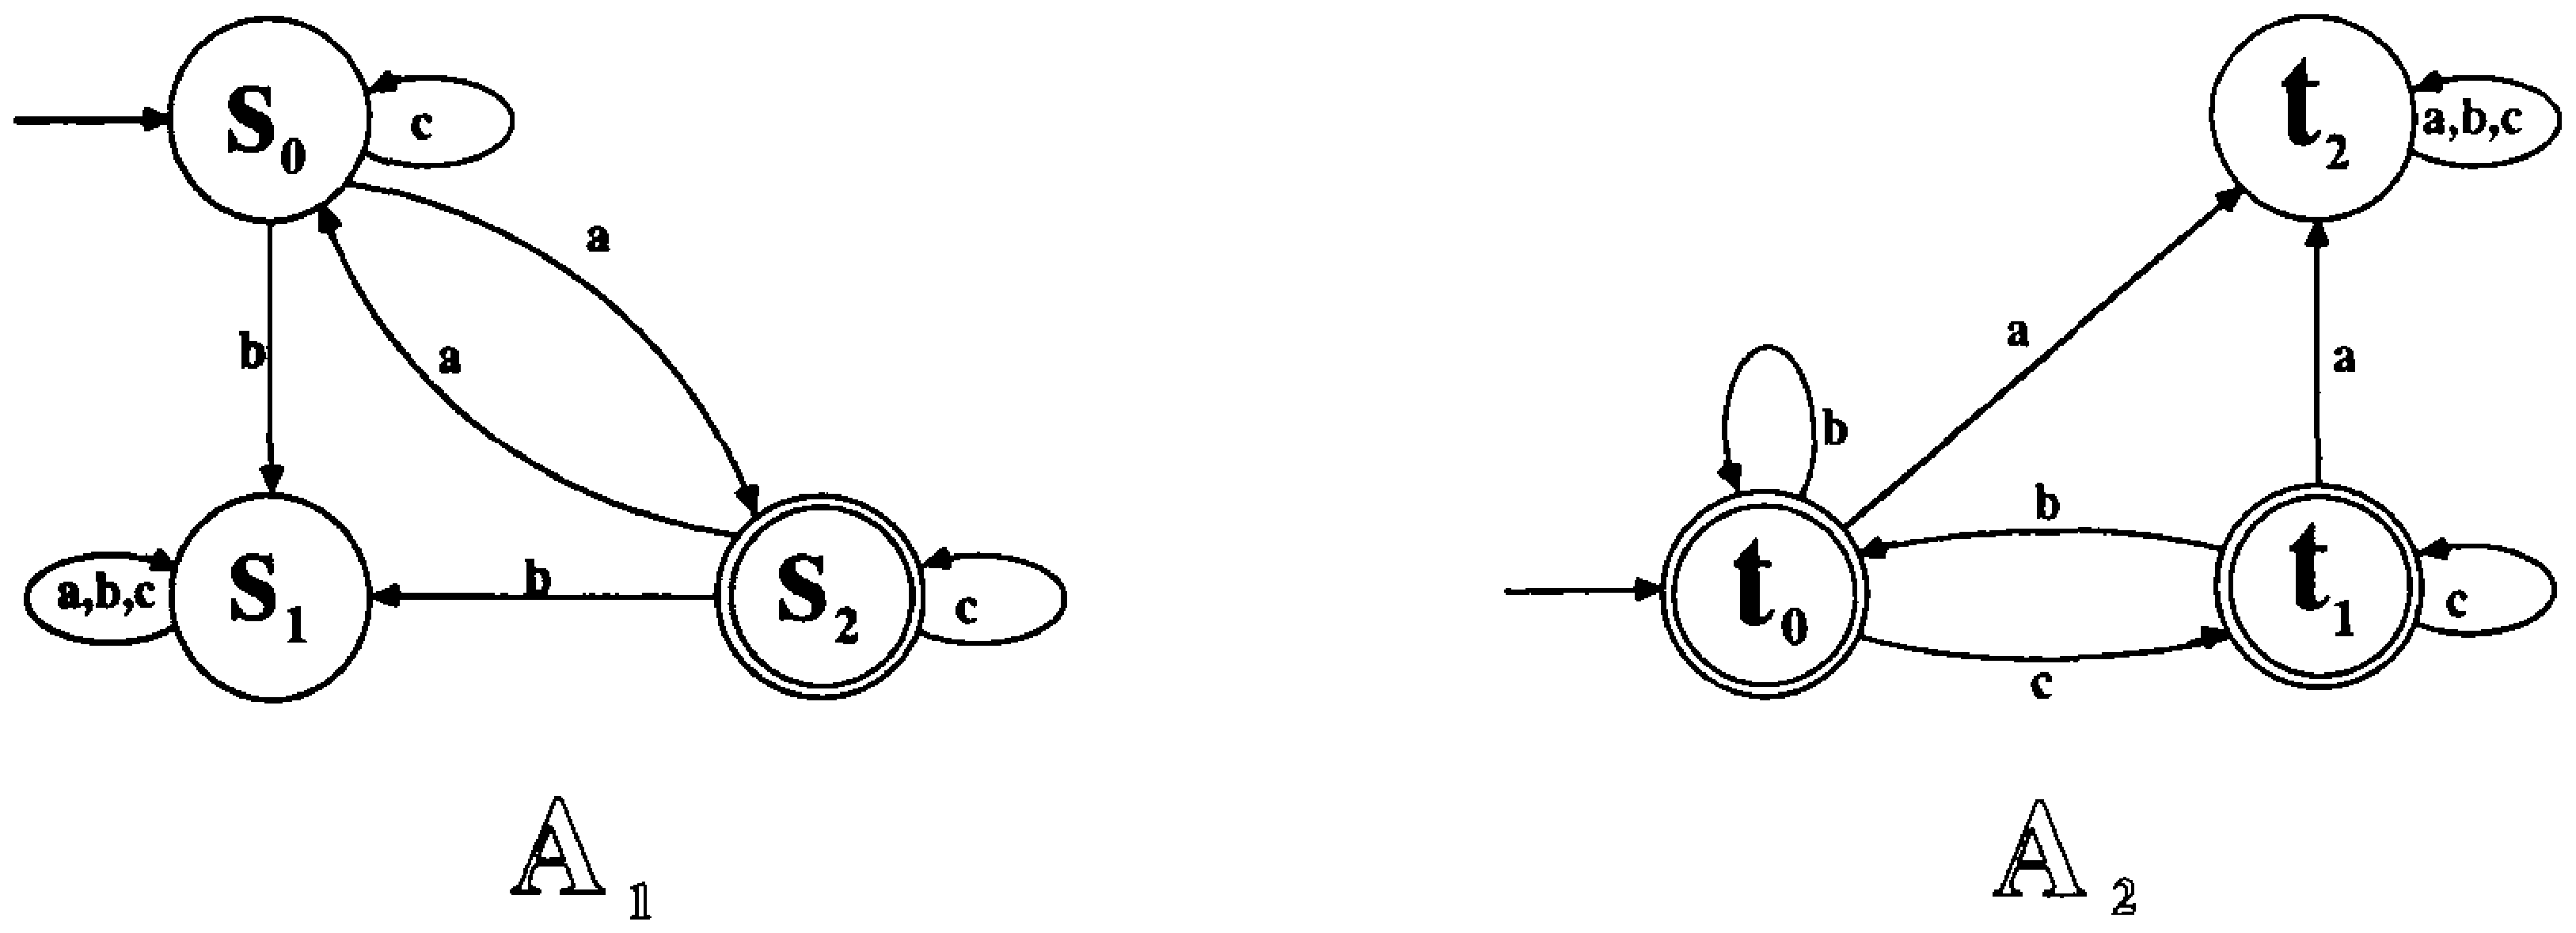
\epsfig{figure=ToFAfigures/fig5-7.eps,width=6in}}
\caption{A pair of candidates for concatenation}\label{fig-5.7}
\end{figure}

% Figure 5.8
\begin{figure}
\centerline{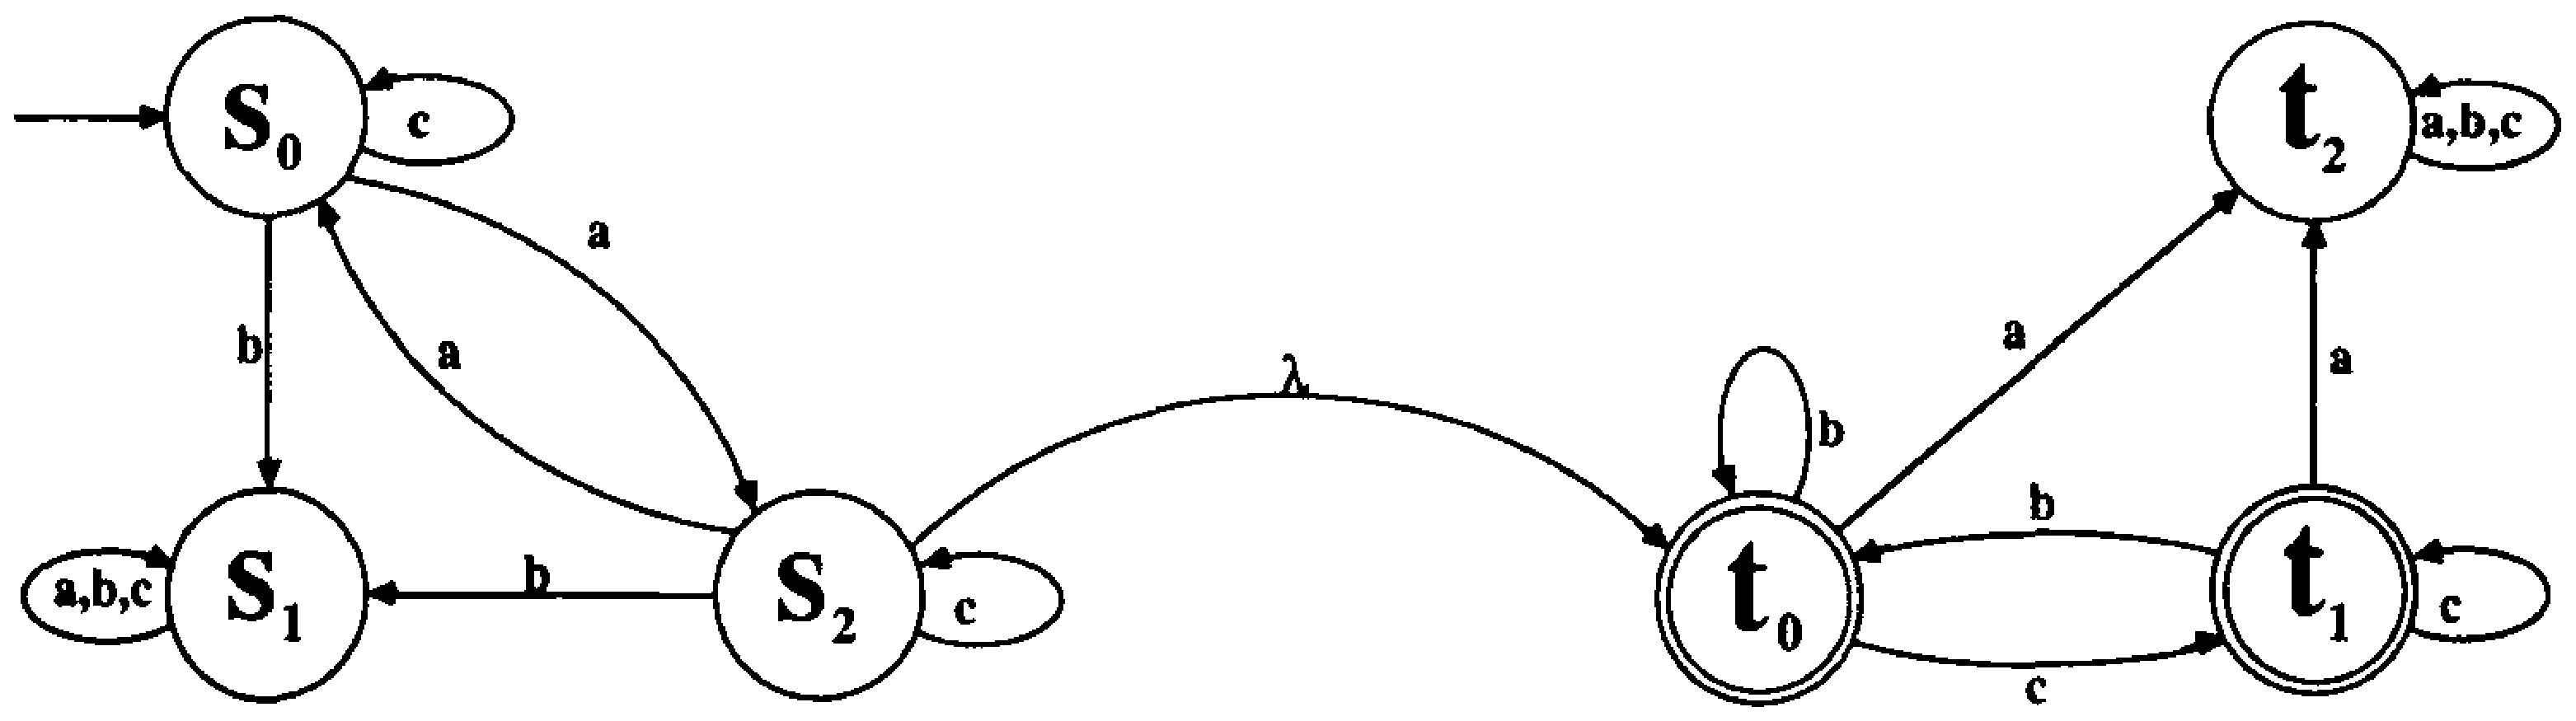
\epsfig{figure=ToFAfigures/fig5-8.eps,width=6in}}
\caption{Concatenation of the machines in Example 5.10 via lambda-moves}\label{fig-5.8}
\end{figure}

It is also possible to directly build a machine for concatenation without using
any $\lambda$-transitions, although the penalty for limiting our attention to
less exotic machines is a loss of clarity in the construction. While the proof
of the following theorem does not depend on $\lambda$-transitions, the resulting
machine is still nondeterministic.

% Theorem 5.4
\begin{thm}\label{thm-5.4}\index{closure!under concatenation}
For any alphabet $\Sigma$, $\DSIG$ is closed under $\cdot$
(concatenation).

\emph{Proof.} Let $L_1$ and $L_2$ belong to $\DSIG$. Then there
are \underline{deterministic} finite automata
$A_1=\langle\Sigma,S_1,s_{0_1},\delta_1,F_1\rangle$ and
$A_2=\langle\Sigma,S_2,s_{0_2},\delta_2,F_2\rangle$ such that $L(A_1)=L_1$ and
$L(A_2)=L_2$. Without loss of generality, assume $S_1 \cap S_2 = \emptyset$.
Define a \underline{non}deterministic machine
$A^\bullet =\langle\Sigma,S^\bullet,S_0^\bullet,\delta^\bullet,F^\bullet\rangle$, where
\begin{center}
\begin{tabular}{ll}
$S^\bullet = S_1 \cup S_2$ & \\ %(without loss of generality, assume
%	$S_1 \cap S_2 = \emptyset$) \\
$S_0^\bullet =\{s_{0_1}\}$ & \\
$F^\bullet = \left\{\begin{array}{l}
			F_2 \\
			F_1 \cup F_2
		  \end{array}\right.$
	& $\begin{array}{l}
		\text{if }\lambda \notin L_2 \\
		\text{if }\lambda \in L_2
	  \end{array}$
\end{tabular}
\end{center}
and $\delta^\bullet$$: (S_1 \cup S_2) \times \Sigma \rightarrow \wp(S_1 \cup S_2)$
is defined by
\begin{center}
\begin{tabular}{l}
$\delta^\bullet(s,\pmb{a})=\left\{\begin{array}{ll}
		\{\delta_1(s,\pmb{a})\} & \text{if }s \in S_1 - F_1 \\
		\{\delta_1(s,\pmb{a}),\delta_2(s_{0_2},\pmb{a})\} & \text{if }s\in F_1 \\
		\{\delta_2(s,\pmb{a})\} & \text{if }s \in S_2
		\end{array}\right.$
\end{tabular}
\end{center}
It can be shown that $L(A^\bullet)=L(A_1)\cdot L(A_2)=L_1 \cdot L_2$ (see the
exercises).
\end{thm}

\subsection*{Example 5.11}

Consider the deterministic finite automata $A_1$ and $A_2$ in Example 5.10. These
can be linked together to form the NDFA $A^\cdot$, and the reader can indeed
verify that the machine illustrated in Figure \ref{fig-5.9} accepts the concatenation of
the languages accepted by $A_1$ and $A_2$. Notice that the new transitions from
the final states of $A_1$ mimic the transitions out of the start state of $A_2$.

Thus we see that avoiding $\lambda$-transitions while defining a concatenation
machine is relatively simple. Unfortunately, avoiding the nondeterministic
aspects of the construction is relatively impractical and would basically entail
re-creating the construction in Definition \ref{dfn-4.5} (which outlined the method for
converting an NDFA into a DFA). Whereas it was merely convenient (rather than
necessary) to employ NDFAs to demonstrate that $\DSIG$ is closed
under union, the use of nondeterminism is essential to the proof of closure
under concatenation.

% Figure 5.9
\begin{figure}
\centerline{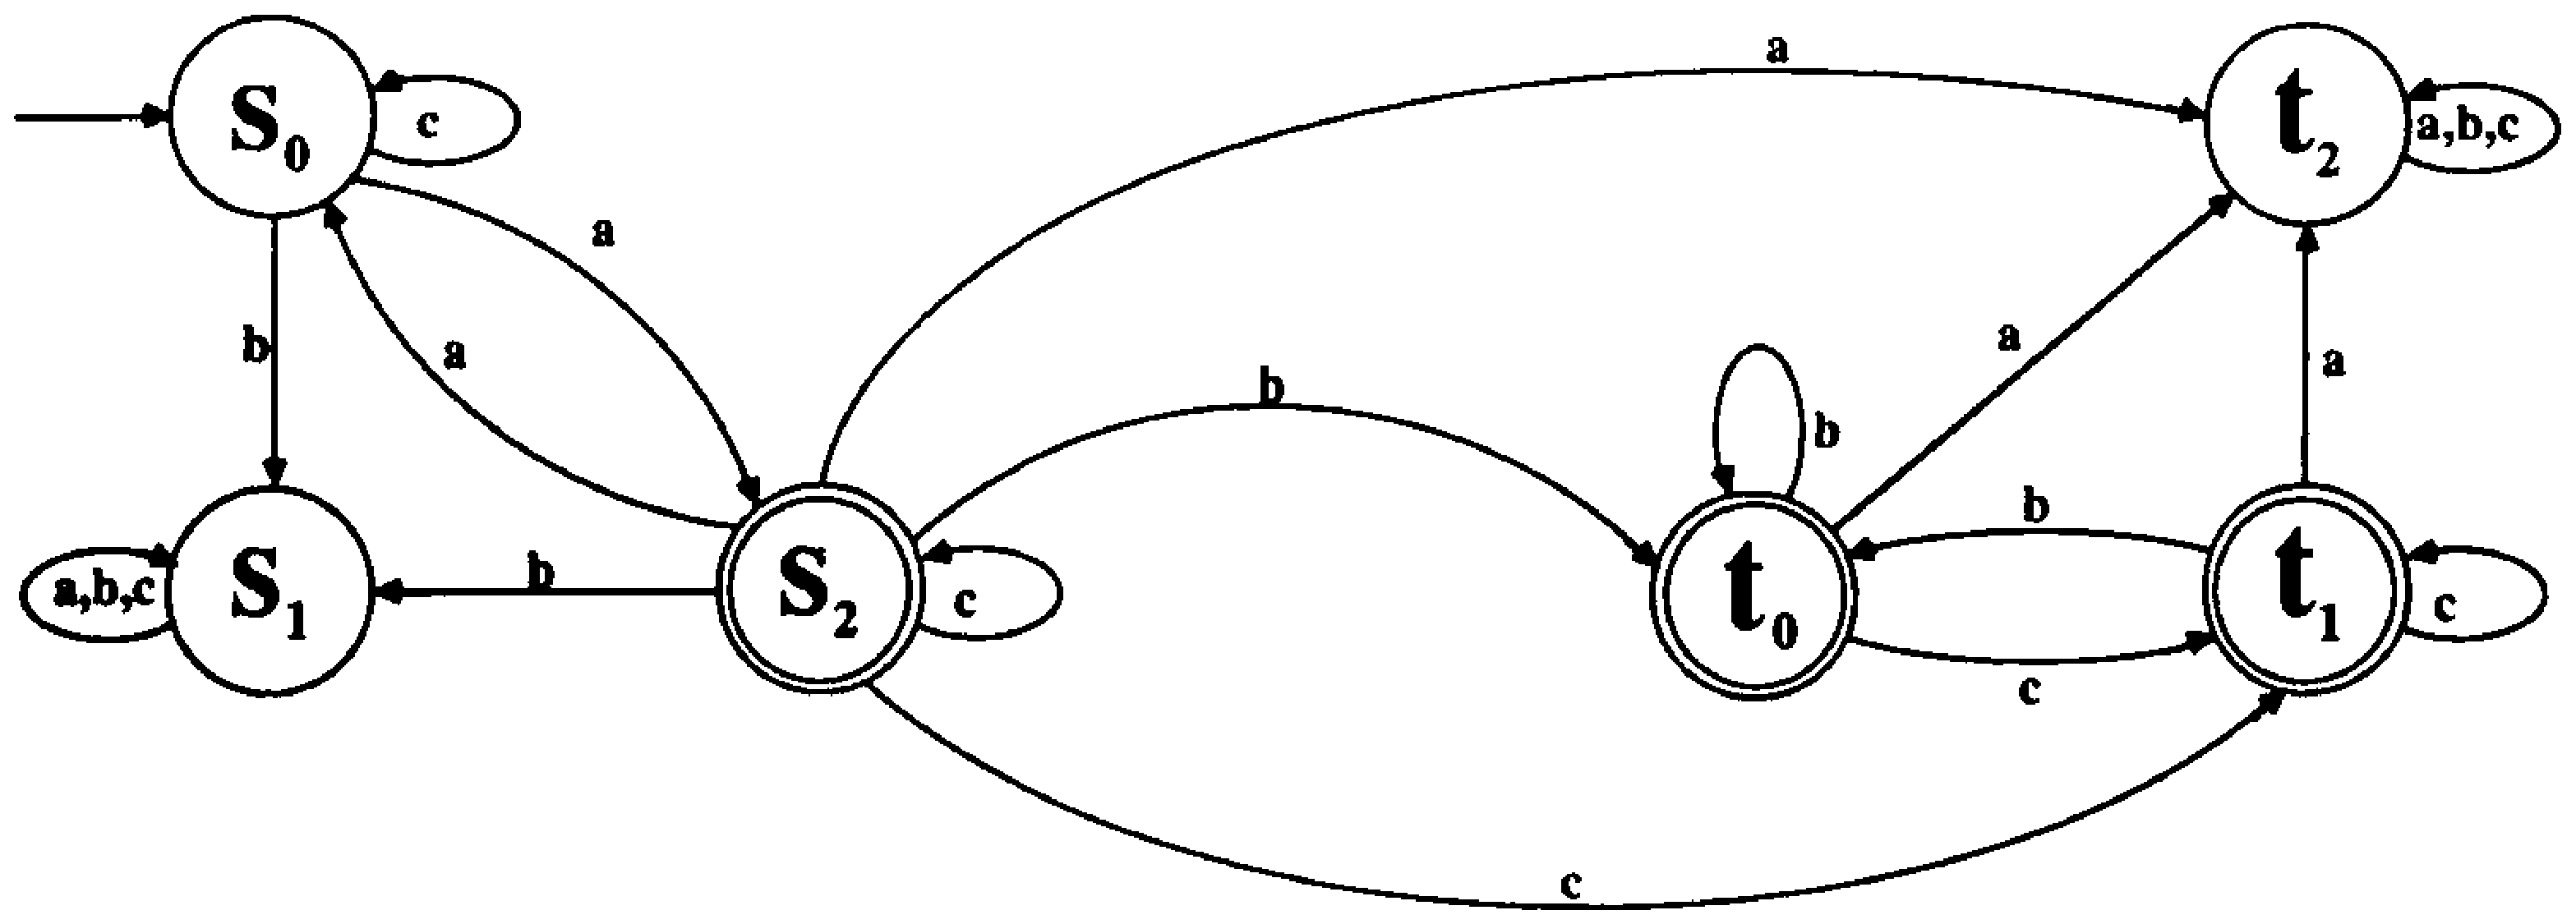
\epsfig{figure=ToFAfigures/fig5-9.eps,width=6in}}
\caption{Concatenation of the machines in Example 5.10 without lambda-moves
(Example 5.11)}\label{fig-5.9}
\end{figure}

\subsection*{Example 5.12}

Consider the nondeterministic finite automata $B_1$ and $B_2$ from Example 5.9.
Applying the analog of Theorem \ref{thm-5.4} (see Exercise 5.43) yields the automaton
shown in Figure \ref{fig-5.10}. Notice that each final state of $B_1$ now also mimics the start
state of $B_2$, and $t_0$ has become a disconnected state. Both $s_0$ and $s_1$
are still final states since $\lambda \in L(B_2)$.

\subsection*{Example 5.13}

Consider the nondeterministic finite automata $B_1$ and $B_3$ shown in Figure
\ref{fig-5.11}, where $B_1$ is the same as that given in Example 5.9, while $B_3$ differs
just slightly from $B_2$ ($t_0$ is no longer a final state). Note that
$L(B_3)=\{\pmb{aa},\pmb{baa}\}$, and $\lambda \notin L(B_3)$. Applying Theorem
\ref{thm-5.4} in this case yields the automaton shown in Figure \ref{fig-5.12}. In this
construction, $s_0$ and $s_1$ are no longer final states since the definition of
$F$ must follow a different rule when $\lambda \notin L(B_3)$. By examining the
resulting machine, the reader can verify that having $t_3$ as the only final
state is indeed the correct strategy for this case.

% Figure 5.10
\begin{figure}
\centerline{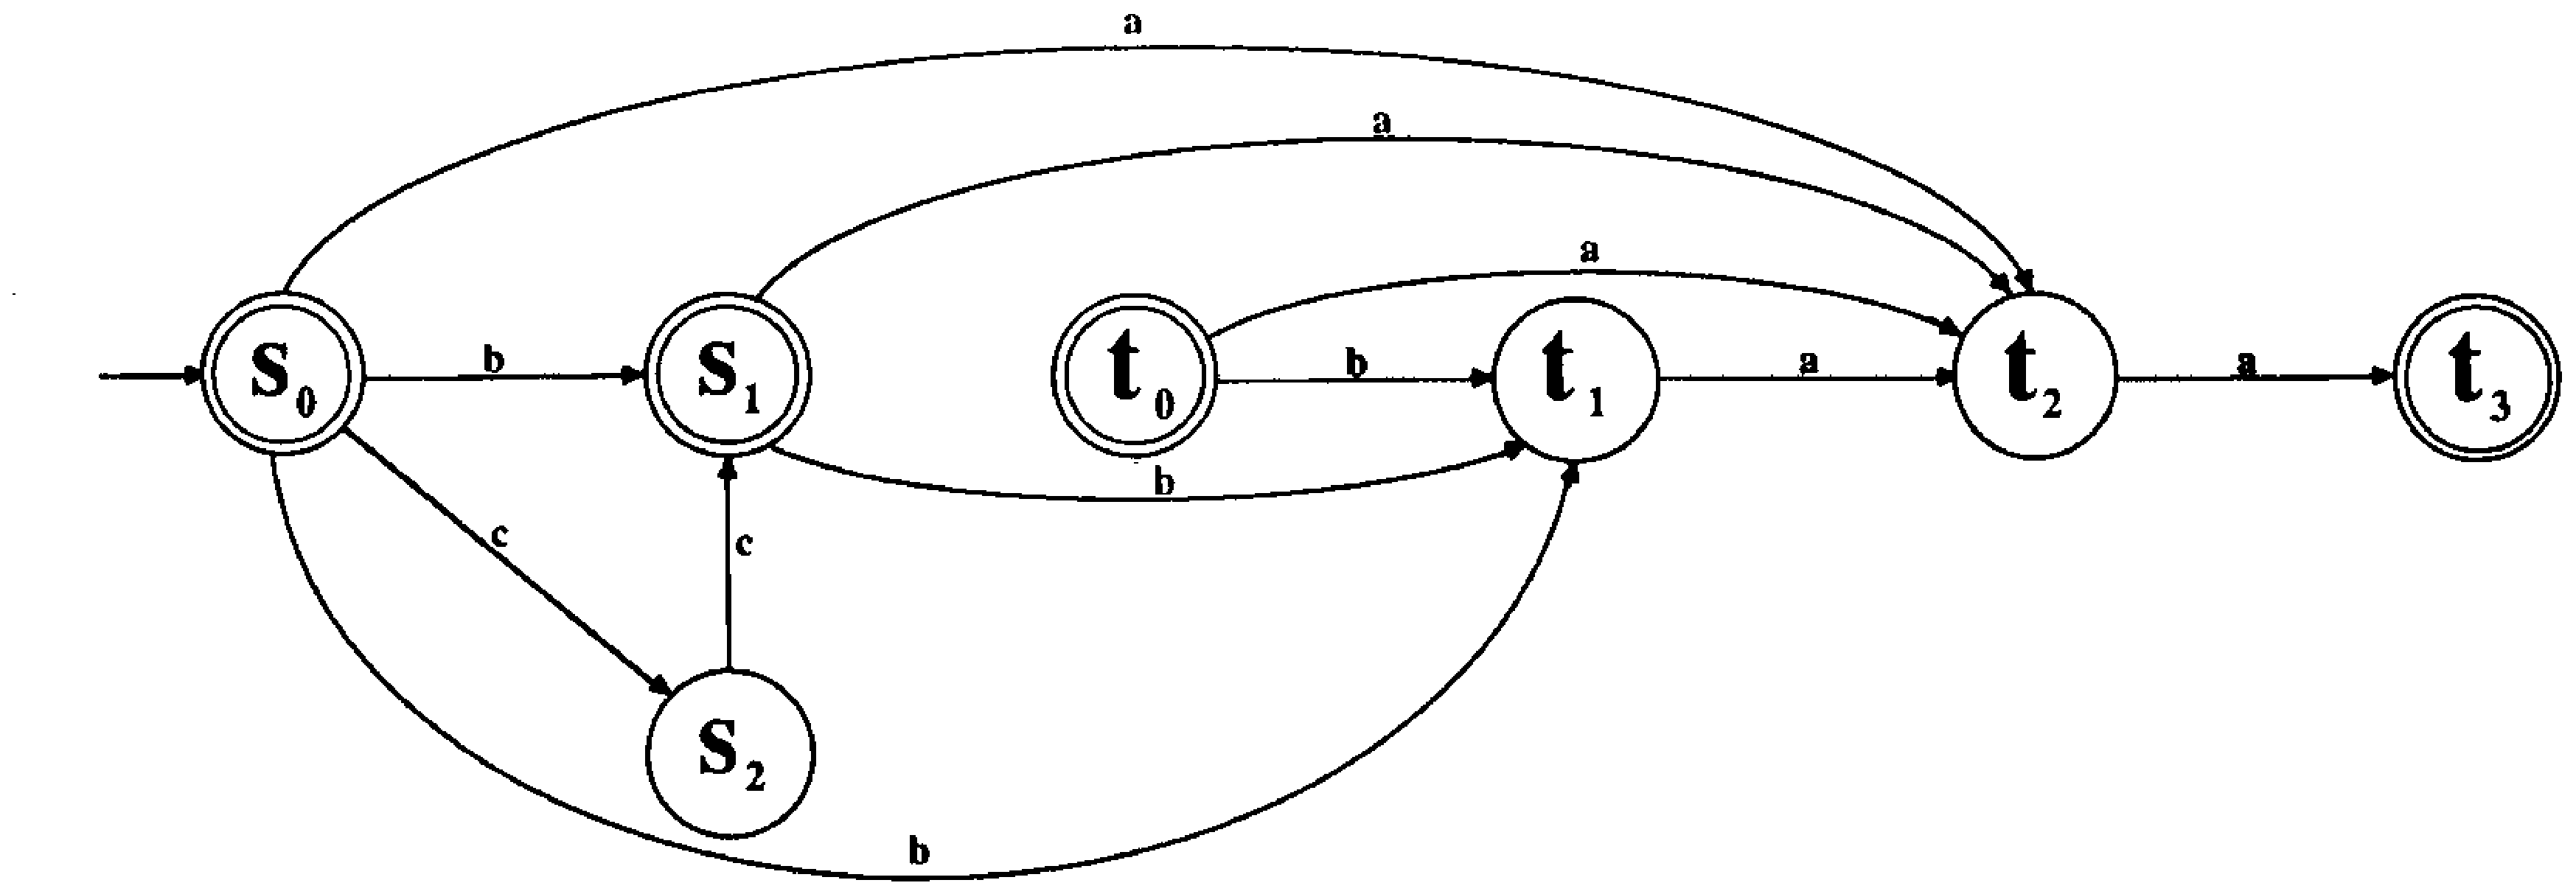
\epsfig{figure=ToFAfigures/fig5-10.eps,width=6in}}
\caption{An NDFA without lambda-moves which accepts the concatenation of the
languages discussed in Example 5.8}\label{fig-5.10}
\end{figure}

% Figure 5.11
\begin{figure}
\centerline{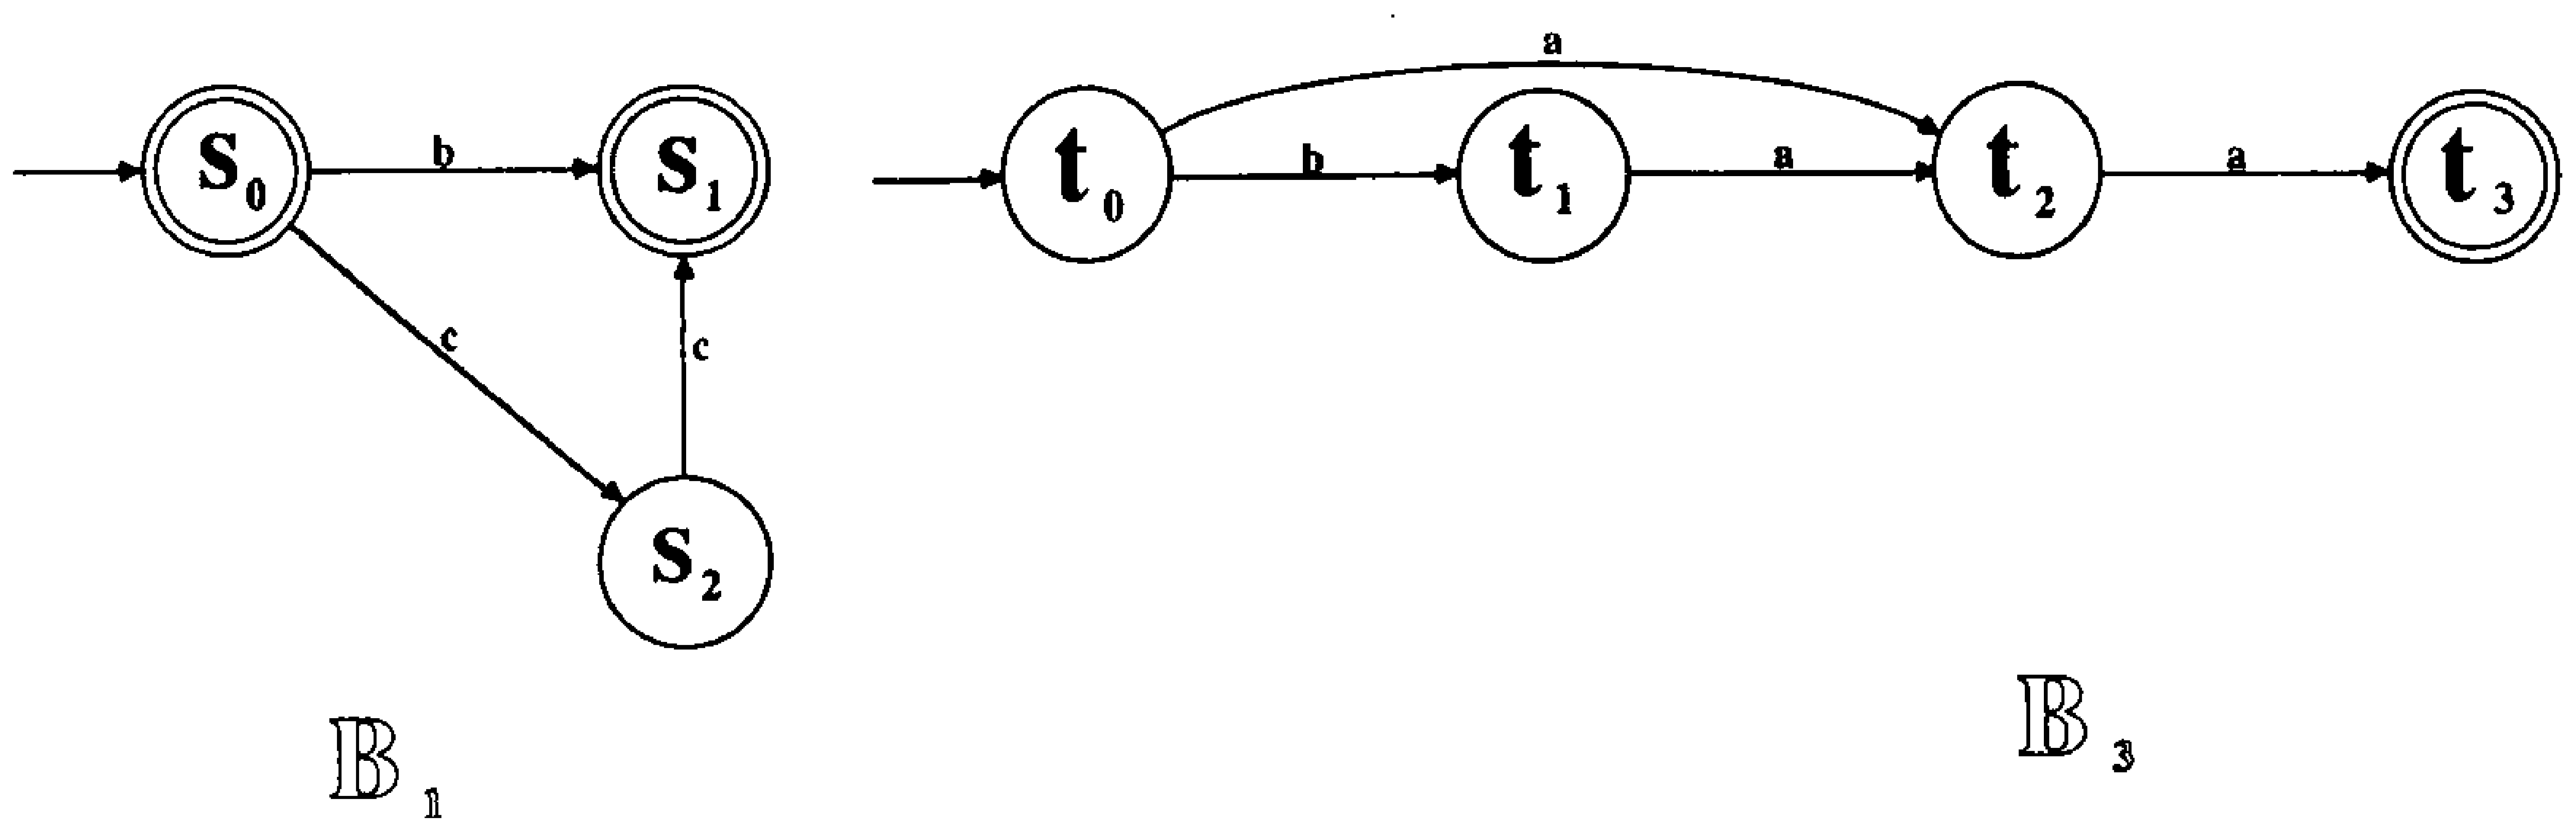
\epsfig{figure=ToFAfigures/fig5-11.eps,width=6in}}
\caption{Candidates for concatenation in which the second machine does not
accept $\lambda$ (Example 5.13)}\label{fig-5.11}
\end{figure}

Besides concatenation, string algebra allows other new operators on languages.
The operators $^*$ and $^+$, which have at this point only been defined for
alphabets, likewise have natural extensions to languages. Loosely, we would
expect $L^*$ to consist of all words that can be formed by the concatenation of
several words from L.
\vspace{1in} % with current spacing, one line of Def5.5 is on page 152,
% followed by two figures at the top of 153, then the rest of Def5.5.  Ugh...

% Figure 5.12
\begin{figure}
\centerline{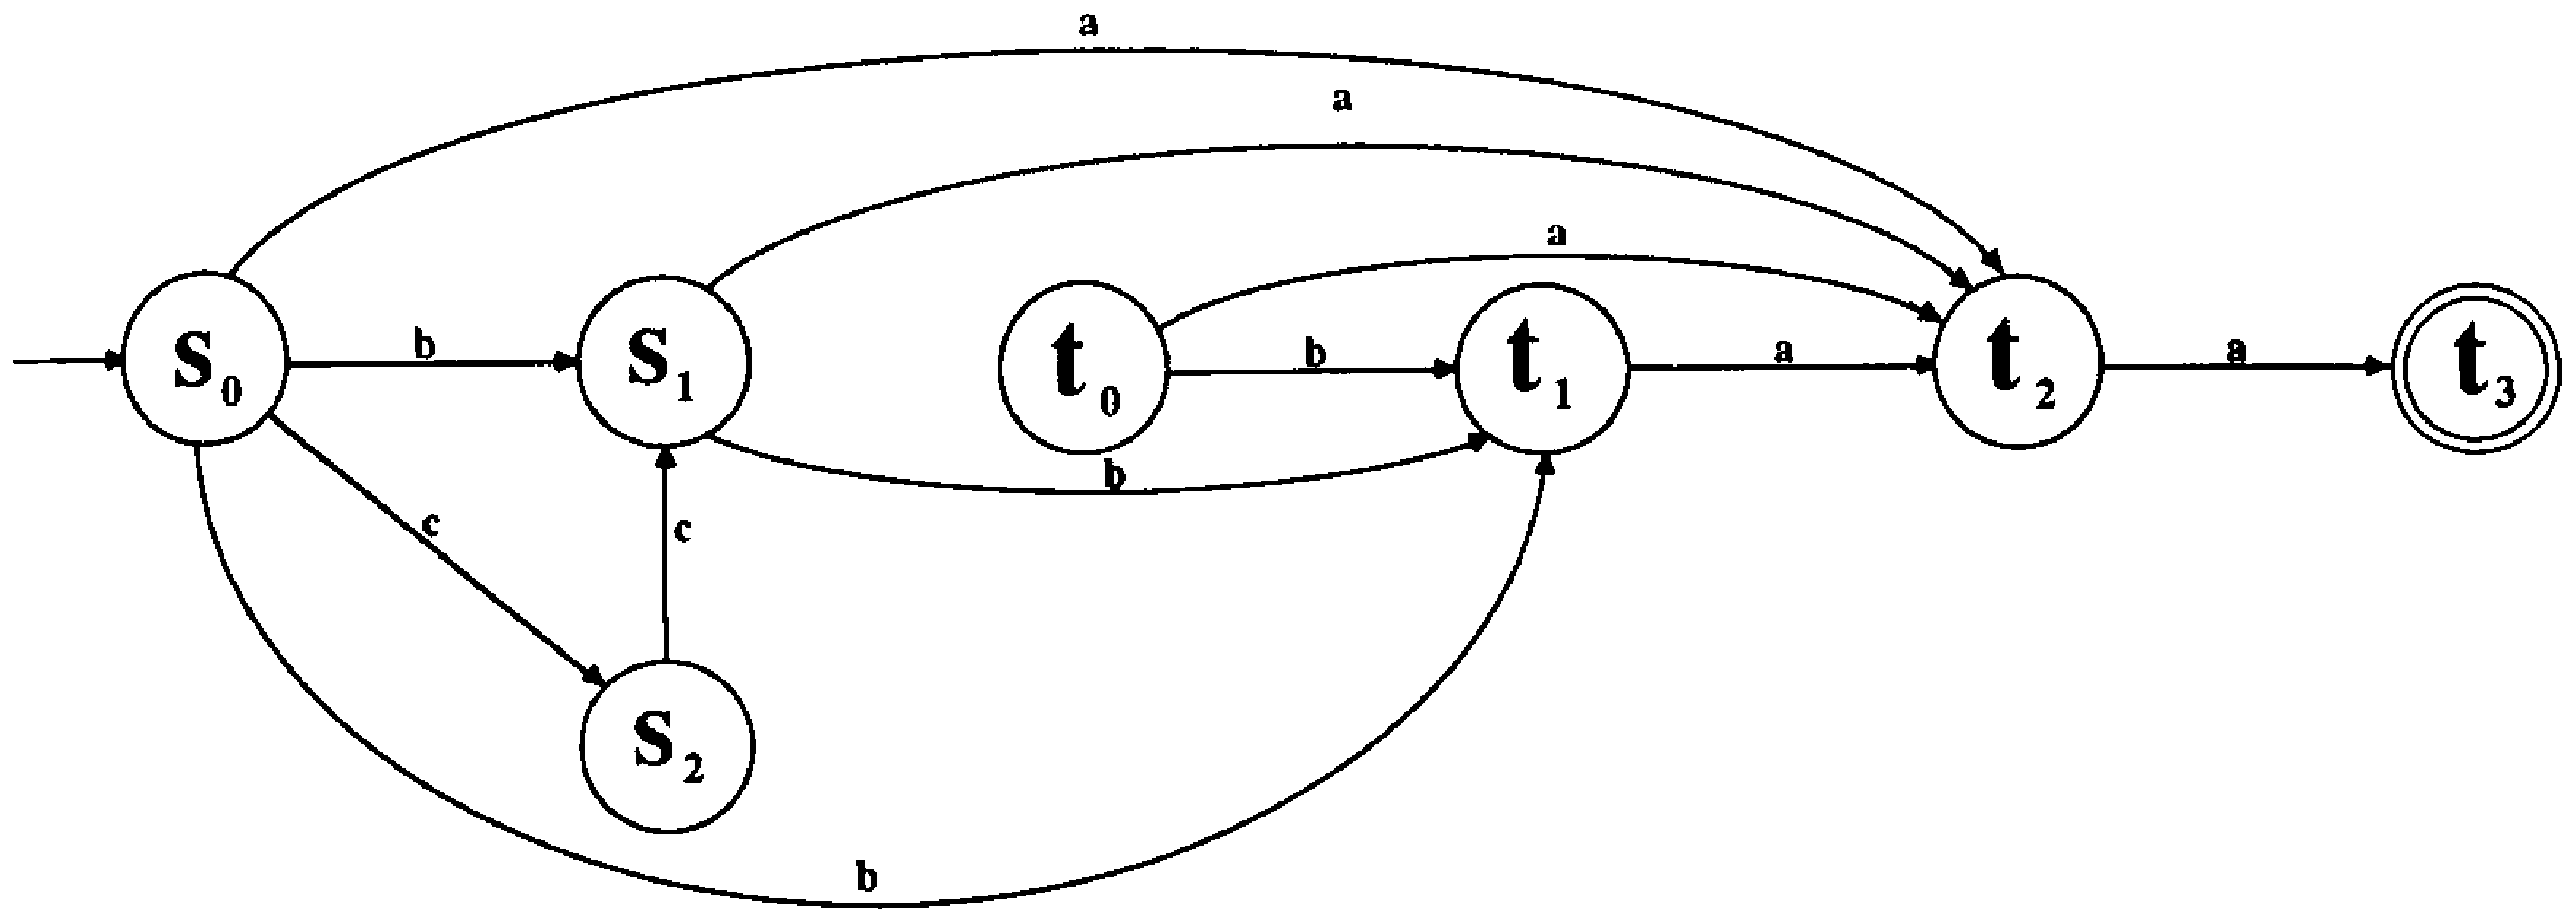
\epsfig{figure=ToFAfigures/fig5-12.eps,width=6in}}
\caption{The concatenation of the NDFAs in Example 5.13}\label{fig-5.12}
\end{figure}

% Definition 5.5
\begin{dfn}\label{dfn-5.5}
Let $L$ be a language over some alphabet $\Sigma$. Define
\begin{center}
\begin{tabular}{l}
$L^0 =\{\lambda\}$ \\
$L^1 = L$ \\
$L^2 = L \cdot L$ \\
$L^3 = L \cdot L^2 = L \cdot L \cdot L$
\end{tabular}
\end{center}
and in general
\begin{center}
\begin{tabular}{l}
$L^n = L\cdot L^{n-1},\qquad \text{for }n = 1,2,3, \ldots$ \\
$L^*= \bigcup\limits^\infty_{i=0} L^i = L^0 \cup L^1 \cup L^2 \cup \cdots =
	\{\lambda\}\cup L\cup L\cdot L\cup L\cdot L\cdot L\cup \ldots$ \\
$L^+= \bigcup\limits^\infty_{i=1} L^i=L^1 \cup L^2 \cup L^3 \cup \cdots =
	L \cup L \cdot L \cup L \cdot L \cdot L \cup \ldots$ \\
\end{tabular}
\end{center}
$L^*$ is called the \emph{\Index{Kleene closure}} of the language $L$.
\end{dfn}

\subsection*{Example 5.14}

If $L =\{\pmb{aa},\pmb{c}\}$, then $L^*=\{\lambda,\pmb{aa},\pmb{c},\pmb{aac},
\pmb{caa},\pmb{aaaa},\pmb{cc},\pmb{aaaaaa},\pmb{aaaac},\pmb{aacaa}, \ldots\}$.

\subsection*{Example 5.15}

If $K =\{\pmb{db},\pmb{b},\pmb{c}\}$, then $K^*$ consists of all words (over
$\{\pmb{b},\pmb{c},\pmb{d}\}$ for which each occurrence of $\pmb{d}$ is immediately followed by (at
least) one $\pmb{b}$.

$\DSIG$ is closed under both $^*$ and $^+$. The technique for
Kleene closure is outlined in Theorem \ref{thm-5.5}. The construction for $L^+$ is similar
(see the exercises).

% Theorem 5.5
\begin{thm}\label{thm-5.5}\index{closure!under Kleene closure}
For any alphabet $\Sigma$, $\DSIG$ is closed under $^*$ (Kleene
closure).

\emph{Proof.} Let L belong to $\DSIG$. Then there is a \underline{non}deterministic
finite automaton $A =\langle\Sigma,S,S_0,\delta,F\rangle$ such that $L(A)=L$.
Define a \underline{non}deterministic machine
$A_*=\langle\Sigma,S_{*},S_{0*},\delta_{*},F_{*}\rangle$,
where
\begin{center}
\begin{tabular}{rll}
$S_{*}=$ & \!\!\!\!$S \cup \{q_0\}\quad \text{(where $q_0$ is some new
	state; $q_0 \notin S$)}$ \\
$S_{0*}=$ &\!\!\!\!$S_0 \cup \{q_0\}$ \\
$F_{*}=$ &\!\!\!\!$F \cup \{q_0\}$
\end{tabular}
\end{center}
and $\delta_{*}$$: (S \cup \{q_0\}) \times \Sigma \rightarrow
	\wp(S \cup \{q_0\})$ is defined by
\[ \delta_{*}(s,\pmb{a}) = \left\{\begin{array}{ll}
		\delta(s,\pmb{a}) & \text{if }s \notin F \cup \{q_0\} \\
		\delta(s,\pmb{a})\cup\left(\bigcup\limits_{t\in S_0}\delta(t,\pmb{a})\right)
			& \text{if }s \in F \\
		\emptyset & \text{if }s = q_0
		\end{array}\right. \]
We claim that $L(A_{*}) = L(A)^* = L^*$ (see the exercises).
\end{thm}

\subsection*{Example 5.16}

Consider the \emph{non}deterministic finite automaton $B$ displayed in Figure 
\ref{fig-5.13}, which accepts all words that contain exactly two (consecutive) $\pmb{b}$s.
Using the modifications described above, the new NDFA $B_{*}$ would look
like the automaton shown in Figure \ref{fig-5.14}. Notice that the new automaton does
indeed accept $L(B)^*$, the set of all words in which the $\pmb{b}$s always occur
in side-by-side pairs. This example also demonstrates the need for the special
extra start (and final) state $q_0$ (see the exercises).

% Figure 5.13
\begin{figure}
\centerline{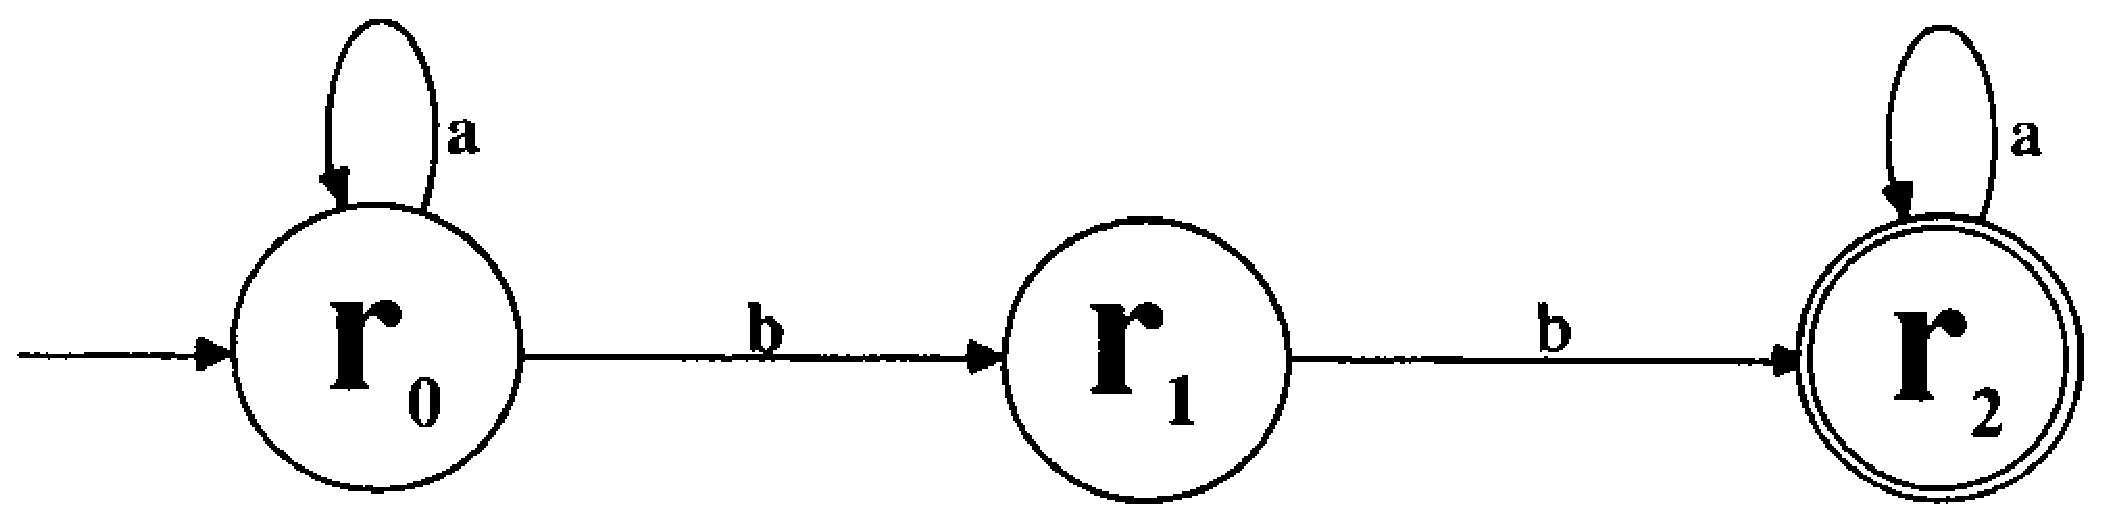
\epsfig{figure=ToFAfigures/fig5-13.eps,width=4in}}
\caption{The NDFA $B$ in Example 5.16.}\label{fig-5.13}
\end{figure}

% Figure 5.14
\begin{figure}
\centerline{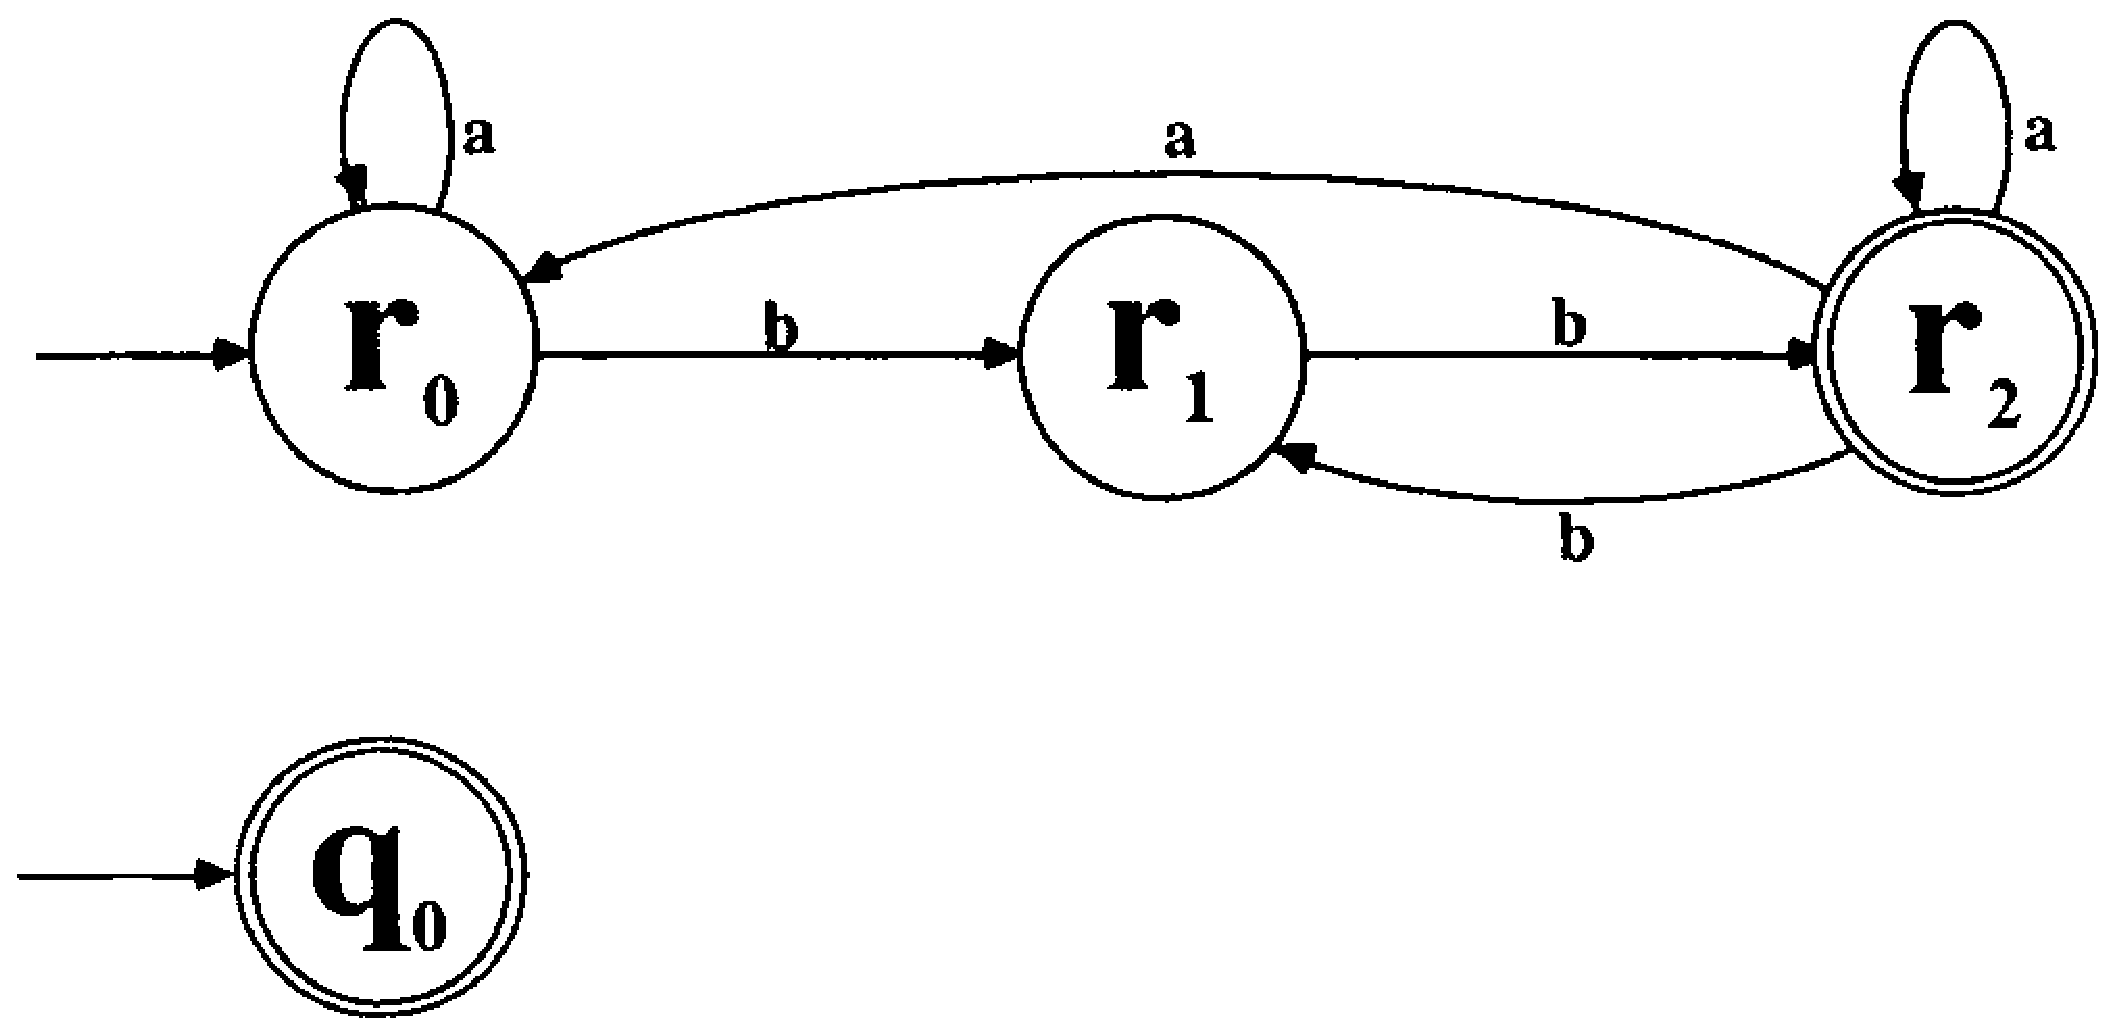
\epsfig{figure=ToFAfigures/fig5-14.eps,width=4in}}
\caption{The resulting NDFA for Example 5.16}\label{fig-5.14}
\end{figure}

It is instructive to compare the different approaches taken in the proofs of
Theorems \ref{thm-5.4} and \ref{thm-5.5}. In both cases, nondeterministic automata were built, but
Theorem \ref{thm-5.4} began with deterministic machines, while Theorem \ref{thm-5.5} assumed that
an NDFA was provided. Note that, in the construction of $\delta^\bullet$ in
Theorem \ref{thm-5.4}, $\delta_1$ was a deterministic transition function and as such
produced a single state, whereas $\delta^\bullet$, on the other hand, must
adhere to the nondeterministic definition and produce a \emph{set} of states. As a
consequence, the definition of $\delta^\bullet$ involved expressions like
$\{\delta_1(s,\pmb{a})\}$, which indicated that the single state given by
$\delta_1(s,\pmb{a})$ should be viewed as a singleton set.

By contrast, Theorem \ref{thm-5.5} specified the nondeterministic transition function
$\delta_{*}$ in terms of $\delta$, which was also assumed to be
nondeterministic. This gave rise to definitions of the form
$\delta_*(s,\pmb{a}) = \delta(s,\pmb{a})$. In this case, no set brackets $\{\ \}$
were necessary since $\delta(s,\pmb{a})$ by assumption already represented a set
(rather than just a single element as in the deterministic case).

The definition of the new set of start states $S_0$ is also affected by the type
of machine from which the new NDFA is formed. In reviewing Theorems \ref{thm-5.4} and \ref{thm-5.5},
the reader should be able to see the parallel between the differences in the
specifications of the $\delta$ function and the differences in the definitions
of $S^\bullet_0$ and $S_{0*}$. It is also instructive to compare and contrast
the proof of Theorem \ref{thm-5.2} to those discussed above.

\section{Further Closure Properties}\label{sec-5.2}

The operators discussed in this section, while not as fundamental as those
presented earlier, illustrate some useful techniques for constructing modified
automata. Also explored are techniques that provide existence proofs rather than
constructive proofs.

% Theorem 5.6
\begin{thm}\label{thm-5.6}
For any alphabet $\Sigma$, $\DSIG$ is closed under the operator Z,
where Z is defined by
\[ Z(L) = \{x \ |\  x \text{ is formed by deleting zero or more letters from a
	word in L}\}. \]

\emph{Proof.} See the exercises and the following example.
\end{thm}

\subsection*{Example 5.17}

Consider the deterministic finite automaton $C$ displayed in Figure \ref{fig-5.15}, which
accepts the language $\{\pmb{a}^n\pmb{b}^m\ |\ n \geq 1,m \geq 1\}.\ Z(L(C))$ would then be
\[ \{\pmb{a}^n\pmb{b}^m\ |\ n \geq 0, m \geq 0\} \]
and can be accepted by modifying $C$ so that every transition in the diagram has
a corresponding $\lambda$-move (allowing that particular letter to be skipped),
as shown in Figure \ref{fig-5.16}.

% Figure 5.15
\begin{figure}
\centerline{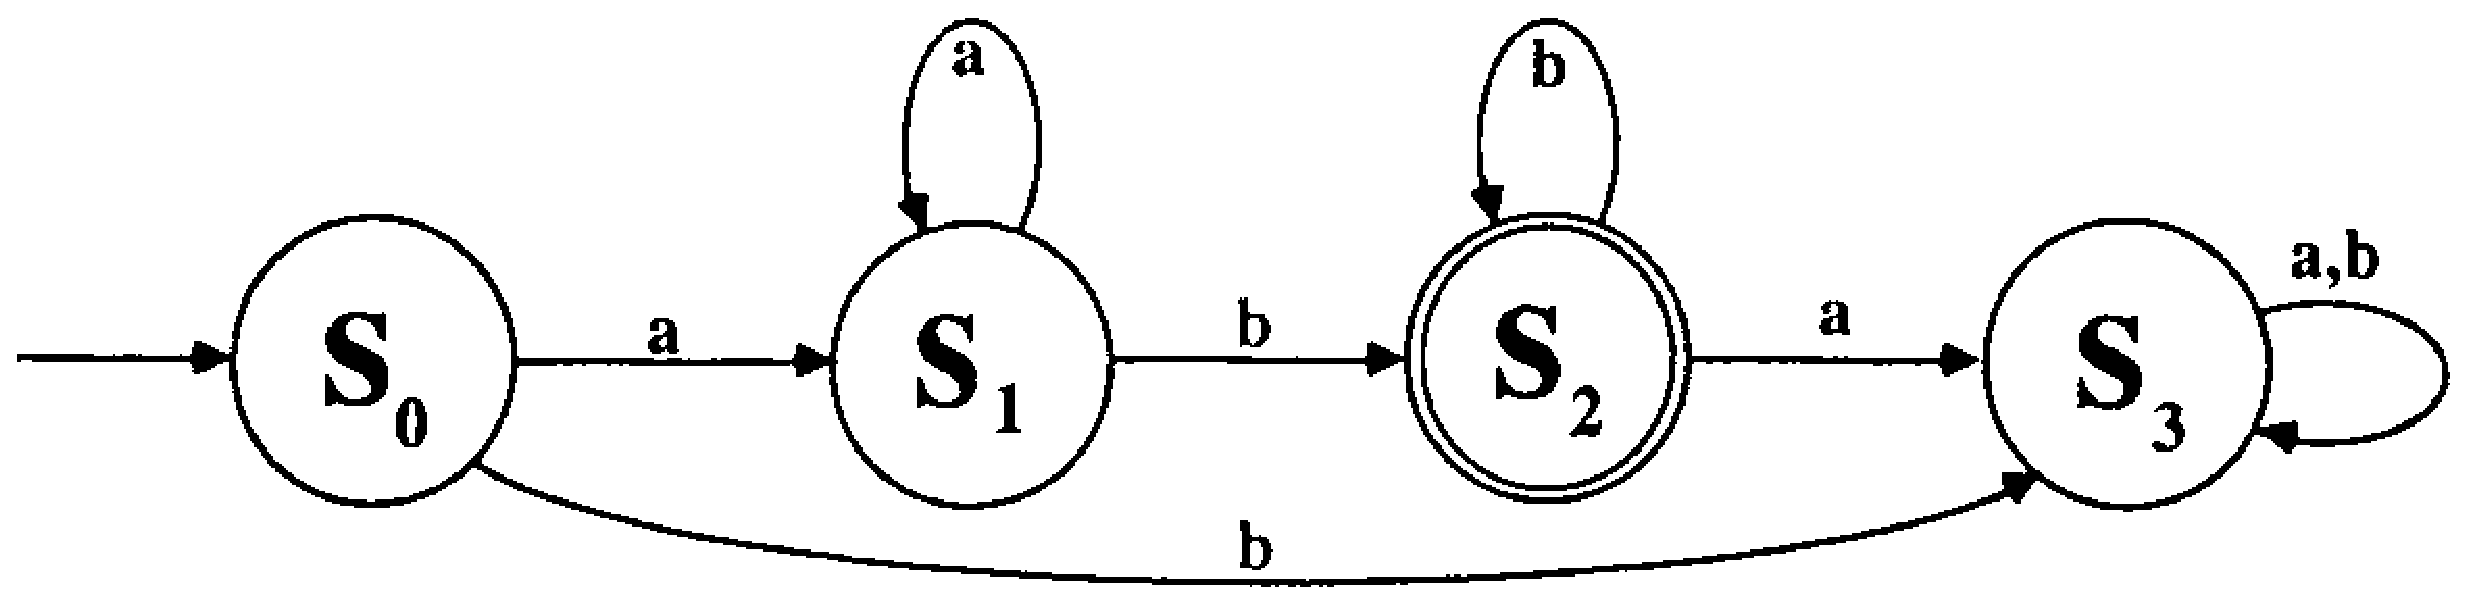
\epsfig{figure=ToFAfigures/fig5-15.eps,width=5in}}
\caption{The automaton $C$ discussed in Example 5.17}\label{fig-5.15}
\end{figure}

% Figure 5.16
\begin{figure}
\centerline{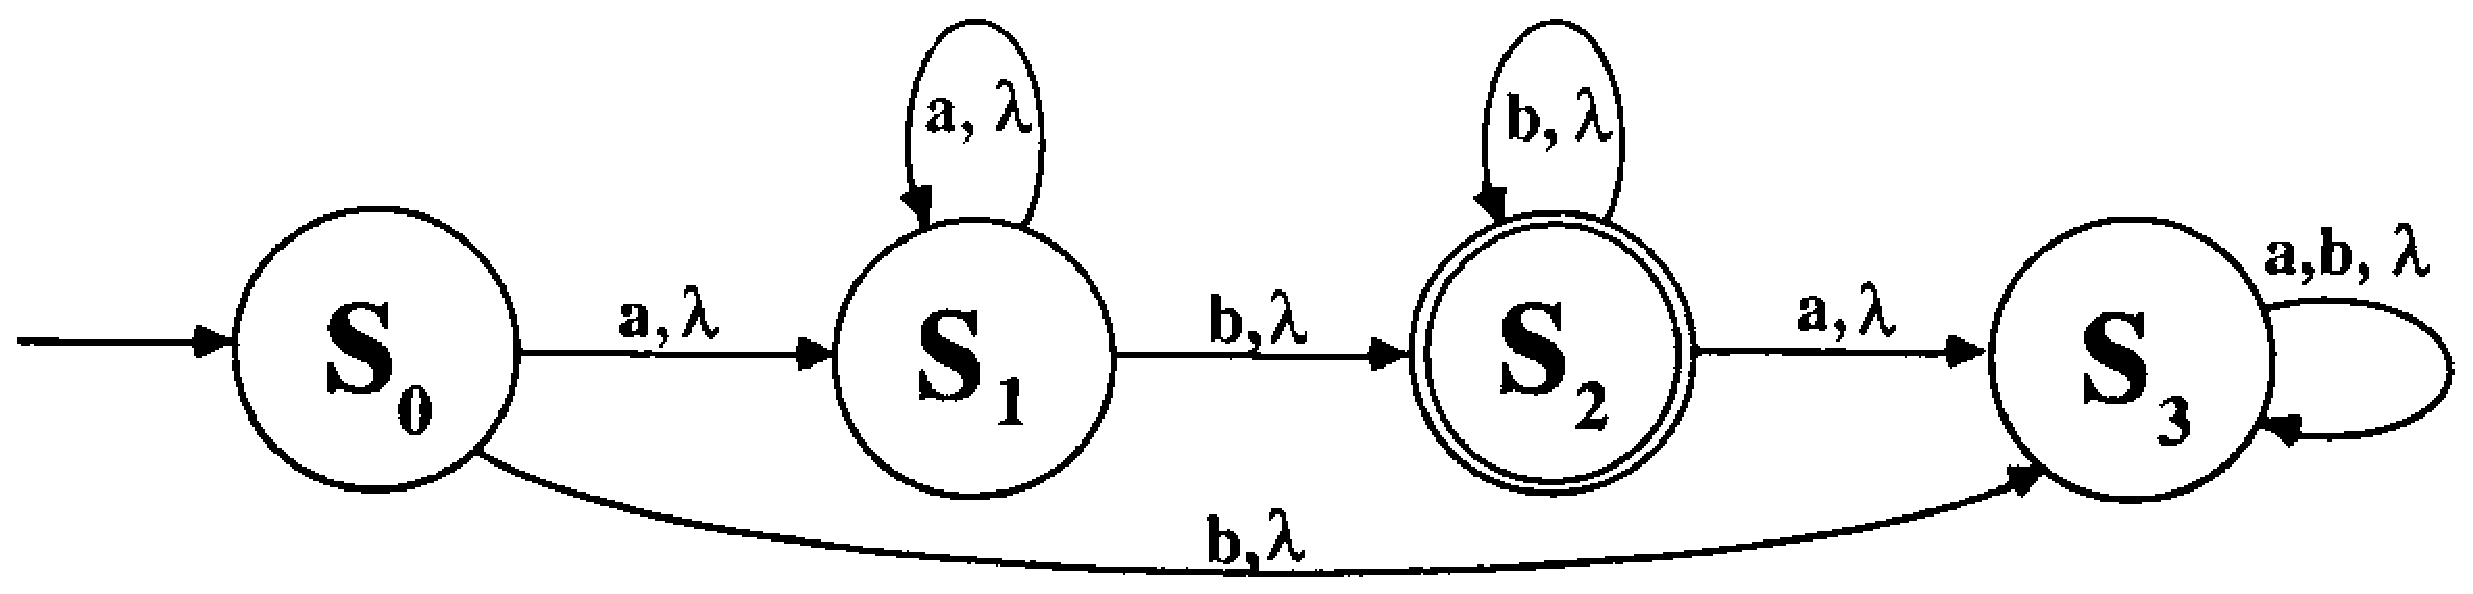
\epsfig{figure=ToFAfigures/fig5-16.eps,width=5in}}
\caption{An automaton accepting $Z(C)$ in Example 5.17}\label{fig-5.16}
\end{figure}

% Figure 5.17
\begin{figure}
\centerline{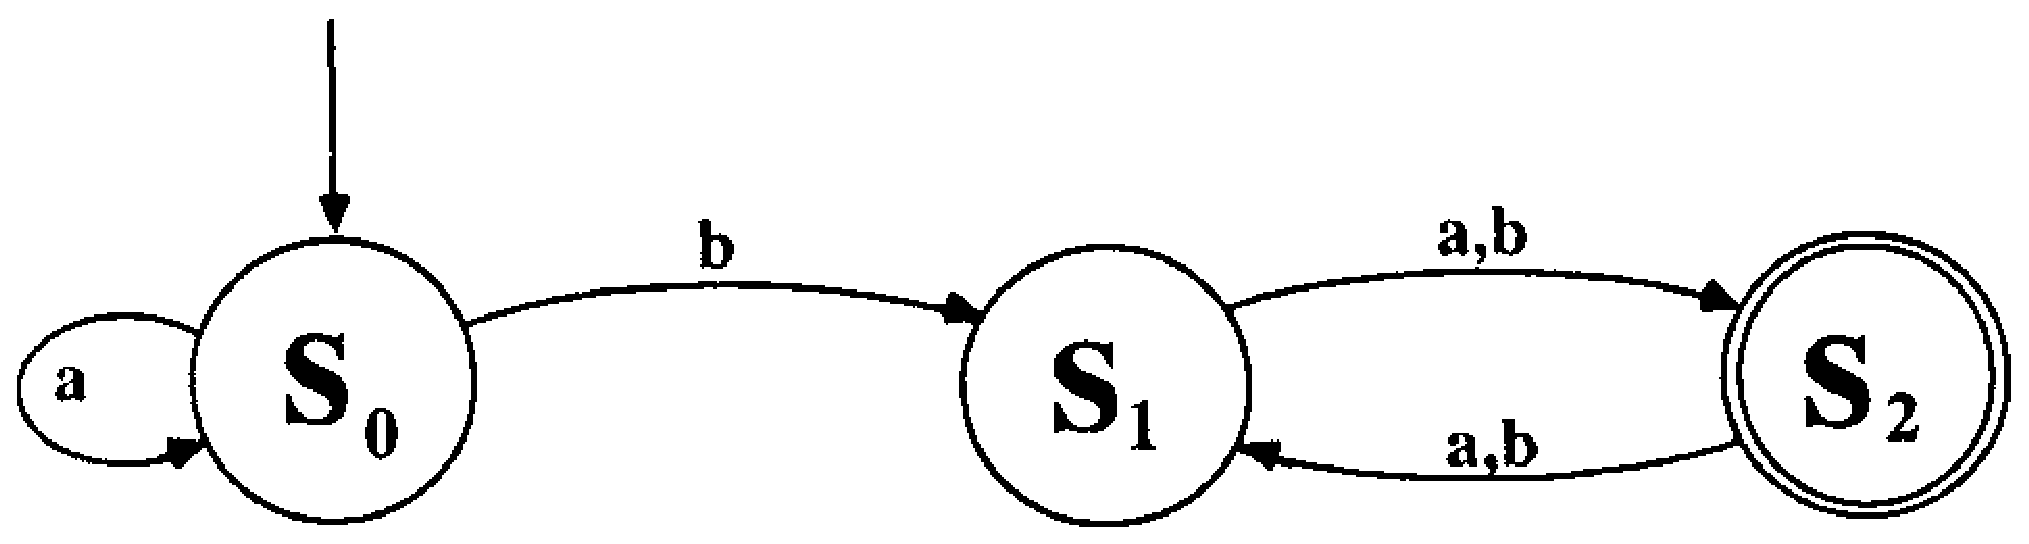
\epsfig{figure=ToFAfigures/fig5-17.eps,width=4in}}
\caption{The automaton $D$ discussed in Example 5.18}\label{fig-5.17}
\end{figure}

% Theorem 5.7
\begin{thm}\label{thm-5.7}
For any alphabet $\Sigma$, $\DSIG$ is closed under the operator
$Y$, where $Y$ is defined by
\[ Y(L) =\{x\ |\ x \text{ is formed by deleting exactly one letter from a
	word in L}\}. \]
\emph{Proof.} See the exercises and the following example.
\end{thm}

\subsection*{Example 5.18}

We need a way to skip a letter as was done in Example 5.17, but we must now
skip one and only one letter. The technique for accomplishing this involves
using \emph{copies} of the original machine. Consider the deterministic finite
automaton $D$ displayed in Figure \ref{fig-5.17}. We will use $\lambda$-moves to mimic
normal transitions, but in this case we will move from one copy of the machine
to an appropriate state in a second copy. Being in the first copy of the machine
will indicate that we have yet to skip a letter, and being in the second copy
will signify that we have followed exactly one $\lambda$-move and have thus
skipped exactly one letter. Hence the second copy will be the only one in which
states are deemed final, and the first copy will contain the only start state.
The modified machine for this example might look like the NDFA shown in Figure
\ref{fig-5.18}. The string $\pmb{aba}$, which is accepted by the original machine, should
cause $\pmb{ab}$, $\pmb{aa}$, and $\pmb{ba}$ to be accepted by the new machine. Each
of these three are indeed accepted, by following the correct $\lambda$-move at
the appropriate time. A similar technique, with the state transition function
slightly redefined, could be used to accept words in which every other letter
was deleted. If one wished only to acknowledge every third letter, three copies
of the machine could be suitably connected together to achieve the desired
result (see the exercises).

% Figure 5.18
\begin{figure}
\centerline{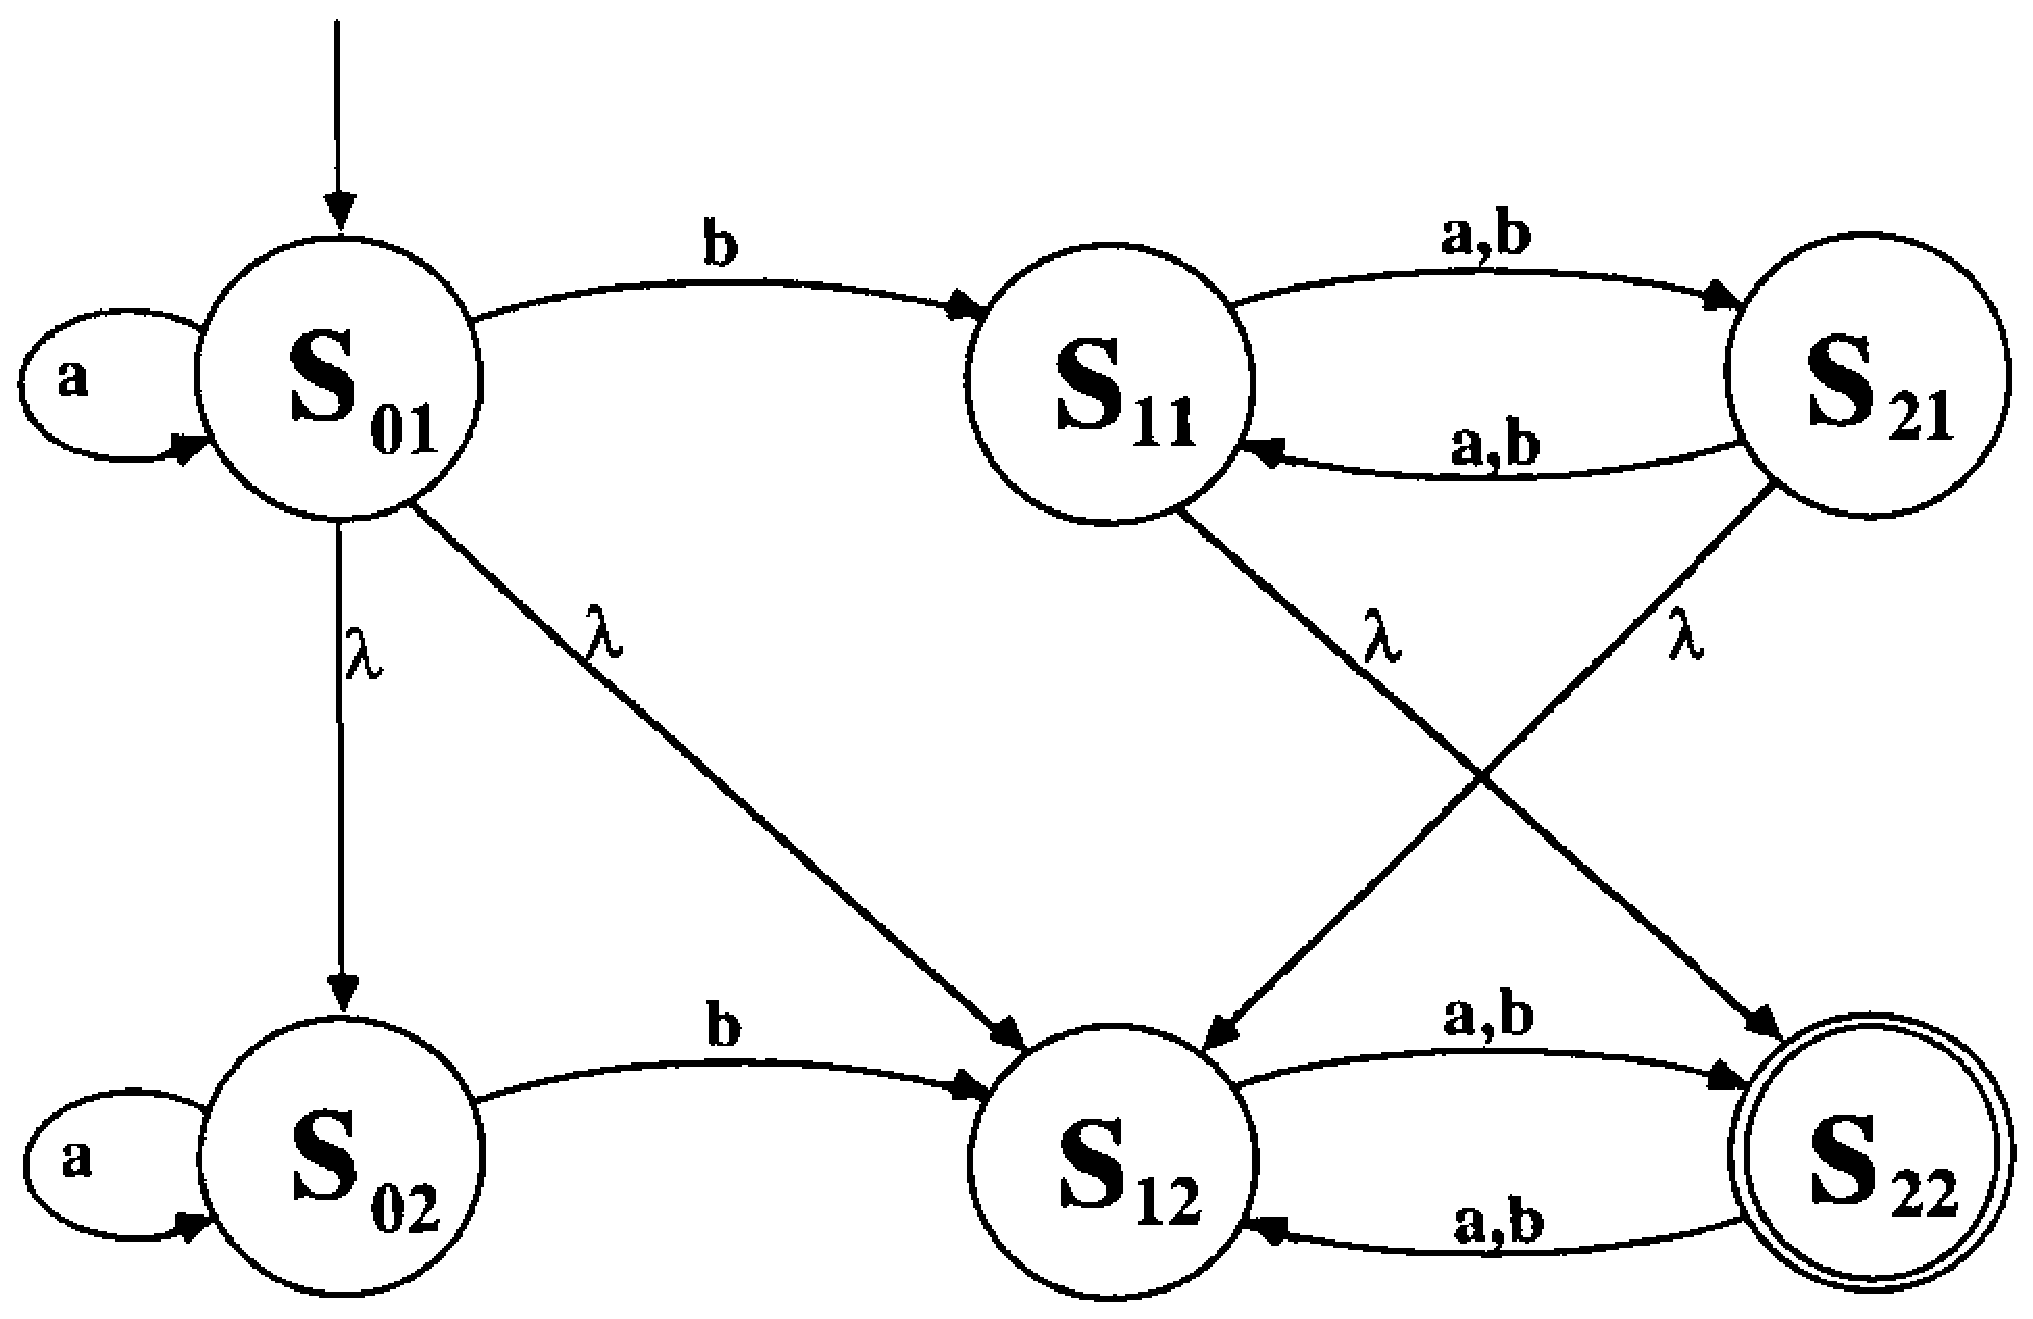
\epsfig{figure=ToFAfigures/fig5-18.eps,width=4in}}
\caption{The modified machine in Example 5.18}\label{fig-5.18}
\end{figure}

While $\DSIG$ is certainly the most important class of languages we have seen so
far, we will now consider some other classes whose properties can be
investigated. The closure properties of other collections of languages will be
considered in the exercises and in later chapters.

% Definition 5.6
\begin{dfn}\label{dfn-5.6}\index{W@\WSIG \ (W-sigma )}
Let $\Sigma$ be an alphabet. Then $\WSIG$ is defined to be the set of all
languages over $\Sigma$ recognized by NDFAs; that is,
\[ \WSIG =\{L \subseteq \Sigma^* \ |\ \exists \text{ NDFA } N \ni L(N)
	= L\}.\]
\end{dfn}

% Lemme 5.2
\begin{lmm}\label{lmm-5.2}
Let $\Sigma$ be an alphabet. Then $\WSIG = \DSIG$.

\emph{Proof.} The proof follows immediately from Theorem \ref{thm-4.1} and Exercise 4.25.
\end{lmm}

The reader should note that Lemma \ref{lmm-5.2} simply restates in new terms the
conclusion reached in Chapter \ref{ch-4}, where it was proved that NDFAs were exactly
as powerful as DFAs. More specifically, it was shown that any language that
could be recognized by an NDFA could also be recognized by a DFA, and conversely.
While every subset of $\Sigma^*$ represents a language, those in \DSIG\ have
exhibited many nice properties owing to the convenient representation afforded
by finite automata. We now focus our attention on ``the other languages,'' that
is, those that are \emph{not} in $\DSIG$.

% Definition 5.7
\begin{dfn}\label{dfn-5.7}\index{N@\NSIG \ (N-sigma )}
Let $\Sigma$ be an alphabet. Then $\NSIG$ is defined to be the set of all
\emph{non}-FAD languages over $\Sigma$; that is,
\[ \NSIG =\{L \subseteq \Sigma^*| \text{ there does \emph{not} exist \emph{any} finite
automaton } M \ni L(M) = L\} \]
\end{dfn}

$\NSIG$ is all the ``complicated'' languages (subsets) that can be formed from
$\Sigma^*$; that is, $\NSIG = \wp(\Sigma^*) - \DSIG$. Be careful not to confuse
\NSIG\ with the set of languages that can be recognized by NDFAs (\WSIG\ in
Definition \ref{dfn-5.6}).

% Theorem 5.8
\begin{thm}\label{thm-5.8}\index{closure!under complementation}
Let $\Sigma$ be an alphabet. Then \NSIG\ is closed under $\sim$ (complementation).

\emph{Proof.} (by contradiction): Assume the lemma is not true, which means that
there exists a language $K$ for which
\begin{center}
\begin{tabular}{rl}
$K \in \NSIG\ \wedge \sim\!\! K \notin \NSIG$ & $\Rightarrow$ (by definition of
	\,\NSIG) \\
$\sim\!\! K \in \DSIG$ & $\Rightarrow$ (by Theorem \ref{thm-5.1}) \\
$\sim\!\!(\sim\!\! K) \in \DSIG$ & $\Rightarrow$ (since
	$\sim\!\!(\sim\!\! K)=K$) \\
$K \in \DSIG$ & $\Rightarrow$ (by definition of \,\NSIG) \\
$K \notin \NSIG$ &
\end{tabular}
\end{center}
which contradicts the assumption. Thus the lemma must be true.
\end{thm}

% Lemma 5.3
\begin{lmm}\label{lmm-5.3}\index{closure!under intersection}
$\mathfrak{N}_{\{\pmb{a},\pmb{b}\}}$ is \emph{not} closed under $\cap$.

\emph{Proof.} Let $L_1=\{\pmb{a}^p\ |\ p$ is prime$\}$ and let $L_2=\{\pmb{b}^p\ |\ p$ is prime$\}$.
Then $L_1 \in \mathfrak{N}_{\{\pmb{a},\pmb{b}\}}$, $L_2 \in \mathfrak{N}_{\{\pmb{a},\pmb{b}\}}$ but
$L_1 \cap L_2 = \emptyset \notin \mathfrak{N}_{\{\pmb{a},\pmb{b}\}}$ (why?).
\end{lmm}

As another useful example of closure, we consider the transformation of one
language to another via a \emph{\Index{language homomorphism}}, which represents
the process of consistently replacing each single letter $\pmb{a}_i$, by a word
$w_i$. Such transformations are commonplace in computer science; some
applications expect lines in a text file to be delimited with a carriage
return/line feed pair, while other applications expect only a carriage return.
Stripping away the unwanted line feeds is tantamount to applying a homomorphism
that replaces most ASCII characters by the same symbol, but replaces line feeds
by $\lambda$. Converting all lowercase letters in a file to uppercase is another
common transformation that can be defined by a language homomorphism.

% Definition 5.8
\begin{dfn}\label{dfn-5.8}
Let $\Sigma=\{\pmb{a_1},\pmb{a_2}, \ldots , \pmb{a_m}\}$ be an alphabet and let
$\Gamma$ be a second alphabet. Given words $w_1,$ $w_2,\ldots ,w_m$ over $\Gamma^*$\!\!,
define a \emph{language homomorphism} $\psi$$: \Sigma \rightarrow \Gamma^*$ by
$\psi(\pmb{a}_i) = w_i$ for each $i$, which can be extended to
$\PBAR$$: \Sigma^* \rightarrow \Gamma^*$ by:
\begin{center}
\begin{tabular}{rcl}
$\PBAR(\lambda)$ & $=$ & $\lambda$ \\
$(\forall \pmb{a} \in \Sigma)(\forall x \in \Sigma^*)(\PBAR(\pmb{a}\cdot x)$ & $=$ &
	$\psi(\pmb{a}) \cdot (\PBAR(x)))$
\end{tabular}
\end{center}
\PBAR can be further extended to operate on a language $L$ by defining
\[ \PBAR(L) =\{\PBAR(z) \in \Gamma^* |\  z \in L\} \]
In this context, $\PBAR$$: \wp(\Sigma^*) \rightarrow \wp(\Gamma^*)$.
\end{dfn}

\subsection*{Example 5.19}

Let $\Sigma =\{\pmb{a},\pmb{b}\}$ and $\Gamma =\{\pmb{c},\pmb{d}\}$, and define
$\psi$ by $\psi(\pmb{a})=\pmb{cd}$ and $\psi(\pmb{b})=\pmb{d}$. For
$K=\{\lambda,\pmb{ab},\pmb{bb}\}$, $\psi(K)=\{\lambda,\pmb{cdd},\pmb{dd}\}$,
while for $L=\{\pmb{a},\pmb{b}\}^*$, $\PBAR(L)$ represents all words over
$\{\pmb{c},\pmb{d}\}$ in which every $\pmb{c}$ is immediately followed by $\pmb{d}$.

\subsection*{Example 5.20}

As a second example, let $\Sigma=\{),(\}$ and let $\Gamma$ be the ASCII
alphabet. If $\mu$ is defined by $\mu(() =$ {\bf begin} and $\mu())=$ {\bf end},
then the set $M$ of all strings of matched parentheses maps to $K$, the set of
all matched {\bf begin}-{\bf end} pairs.

A general homomorphism $\psi$ maps a language over $\Sigma$ to a language over
$\Gamma$. However, to consider the closure of \DSIG, we will restrict our
attention for the moment to homomorphisms for which $\Gamma=\Sigma$. It is more
generally true, though, that even for language homomorphisms between two
different alphabets, if $L$ is FAD, the homomorphic image of L is also FAD (see
the exercises).

% Theorem 5.9
\begin{thm}\label{thm-5.9}\index{closure!under language homomorphism}
Let $\Sigma$ be an alphabet, and let $\psi$$: \Sigma \rightarrow \Sigma^*$ be a
language homomorphism. Then \DSIG\ is closed under $\PBAR$.

\emph{Proof.} See the exercises and the following examples. A much more concise
way to handle this transformation will be seen in Chapter \ref{ch-6} when substitutions
are explored.
\end{thm}

If the homomorphism is \emph{\Index{length preserving}}, that is, if it always
maps letters to single letters, it is relatively easy to define a new automaton
from the old one. Indeed, the state transition diagram hardly changes at all;
all transitions marked $\pmb{b}$ are simply relabeled with the new letter $\psi(\pmb{b})$. For
more complex homomorphisms, extra states must be added to accommodate the
processing of the surplus letters. The following two examples illustrate the
appropriate transformation of the state transition function and suggest a
convenient labeling for the new states.

\subsection*{Example 5.21}

Consider the DFA B displayed in Figure \ref{fig-5.19}a. For the homomorphism $\xi$ defined
by $\xi(\pmb{a})=\pmb{a}$ and $\xi(\pmb{b})=\pmb{a}$, the automaton that will
accept $\overline\xi(L(B))$ is shown in Figure \ref{fig-5.19}b. Note that even in simple examples
like this one the resulting automaton can be nondeterministic.

% Figure 5.19
\begin{figure}
\centerline{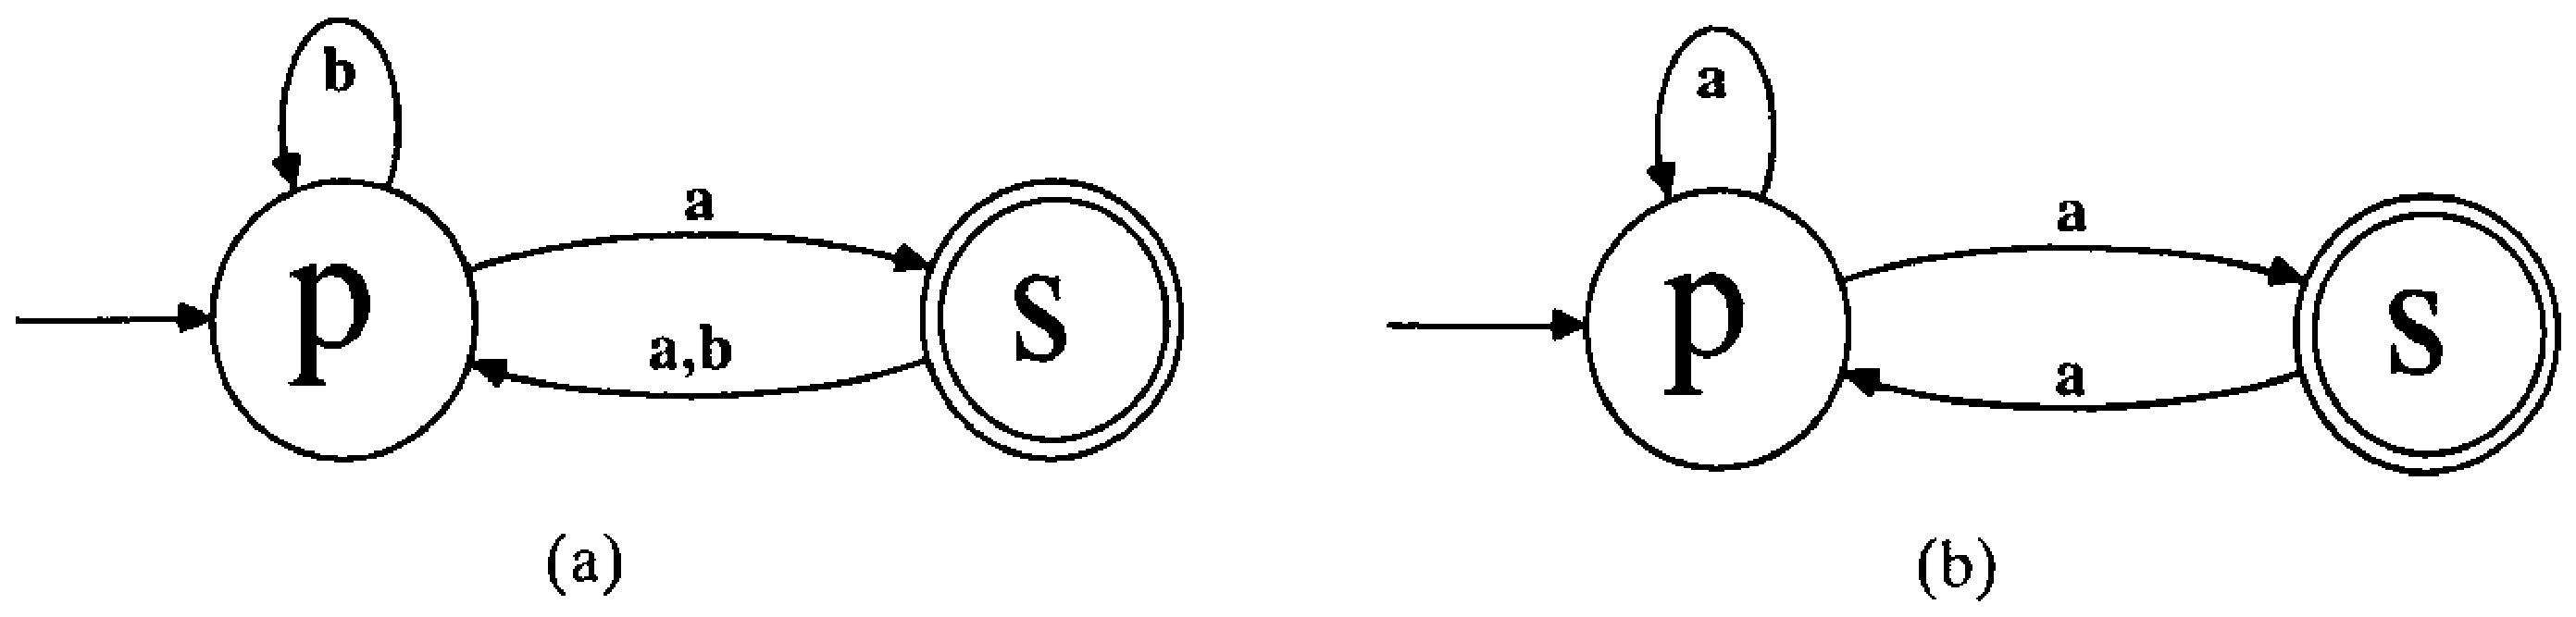
\epsfig{figure=ToFAfigures/fig5-19.eps,width=5.5in}}
\caption{(a) The automaton discussed in Example 5.21; (b) The resulting automaton
for Example 5.21}\label{fig-5.19}
\end{figure}

\subsection*{Example 5.22}

For the NDFA C displayed in Figure \ref{fig-5.20}a and the homomorphism $\mu$ defined by
$\mu(\pmb{a})=\pmb{cc}$ and $\mu(\pmb{b})=\pmb{a}$, the automaton that will
accept $\overline\mu(L(C))$ is shown in Figure \ref{fig-5.20}b. Note that each state of $C$
requires an extra state to accommodate the $\pmb{cc}$ transition.

% Figure 5.20
\begin{figure}
\centerline{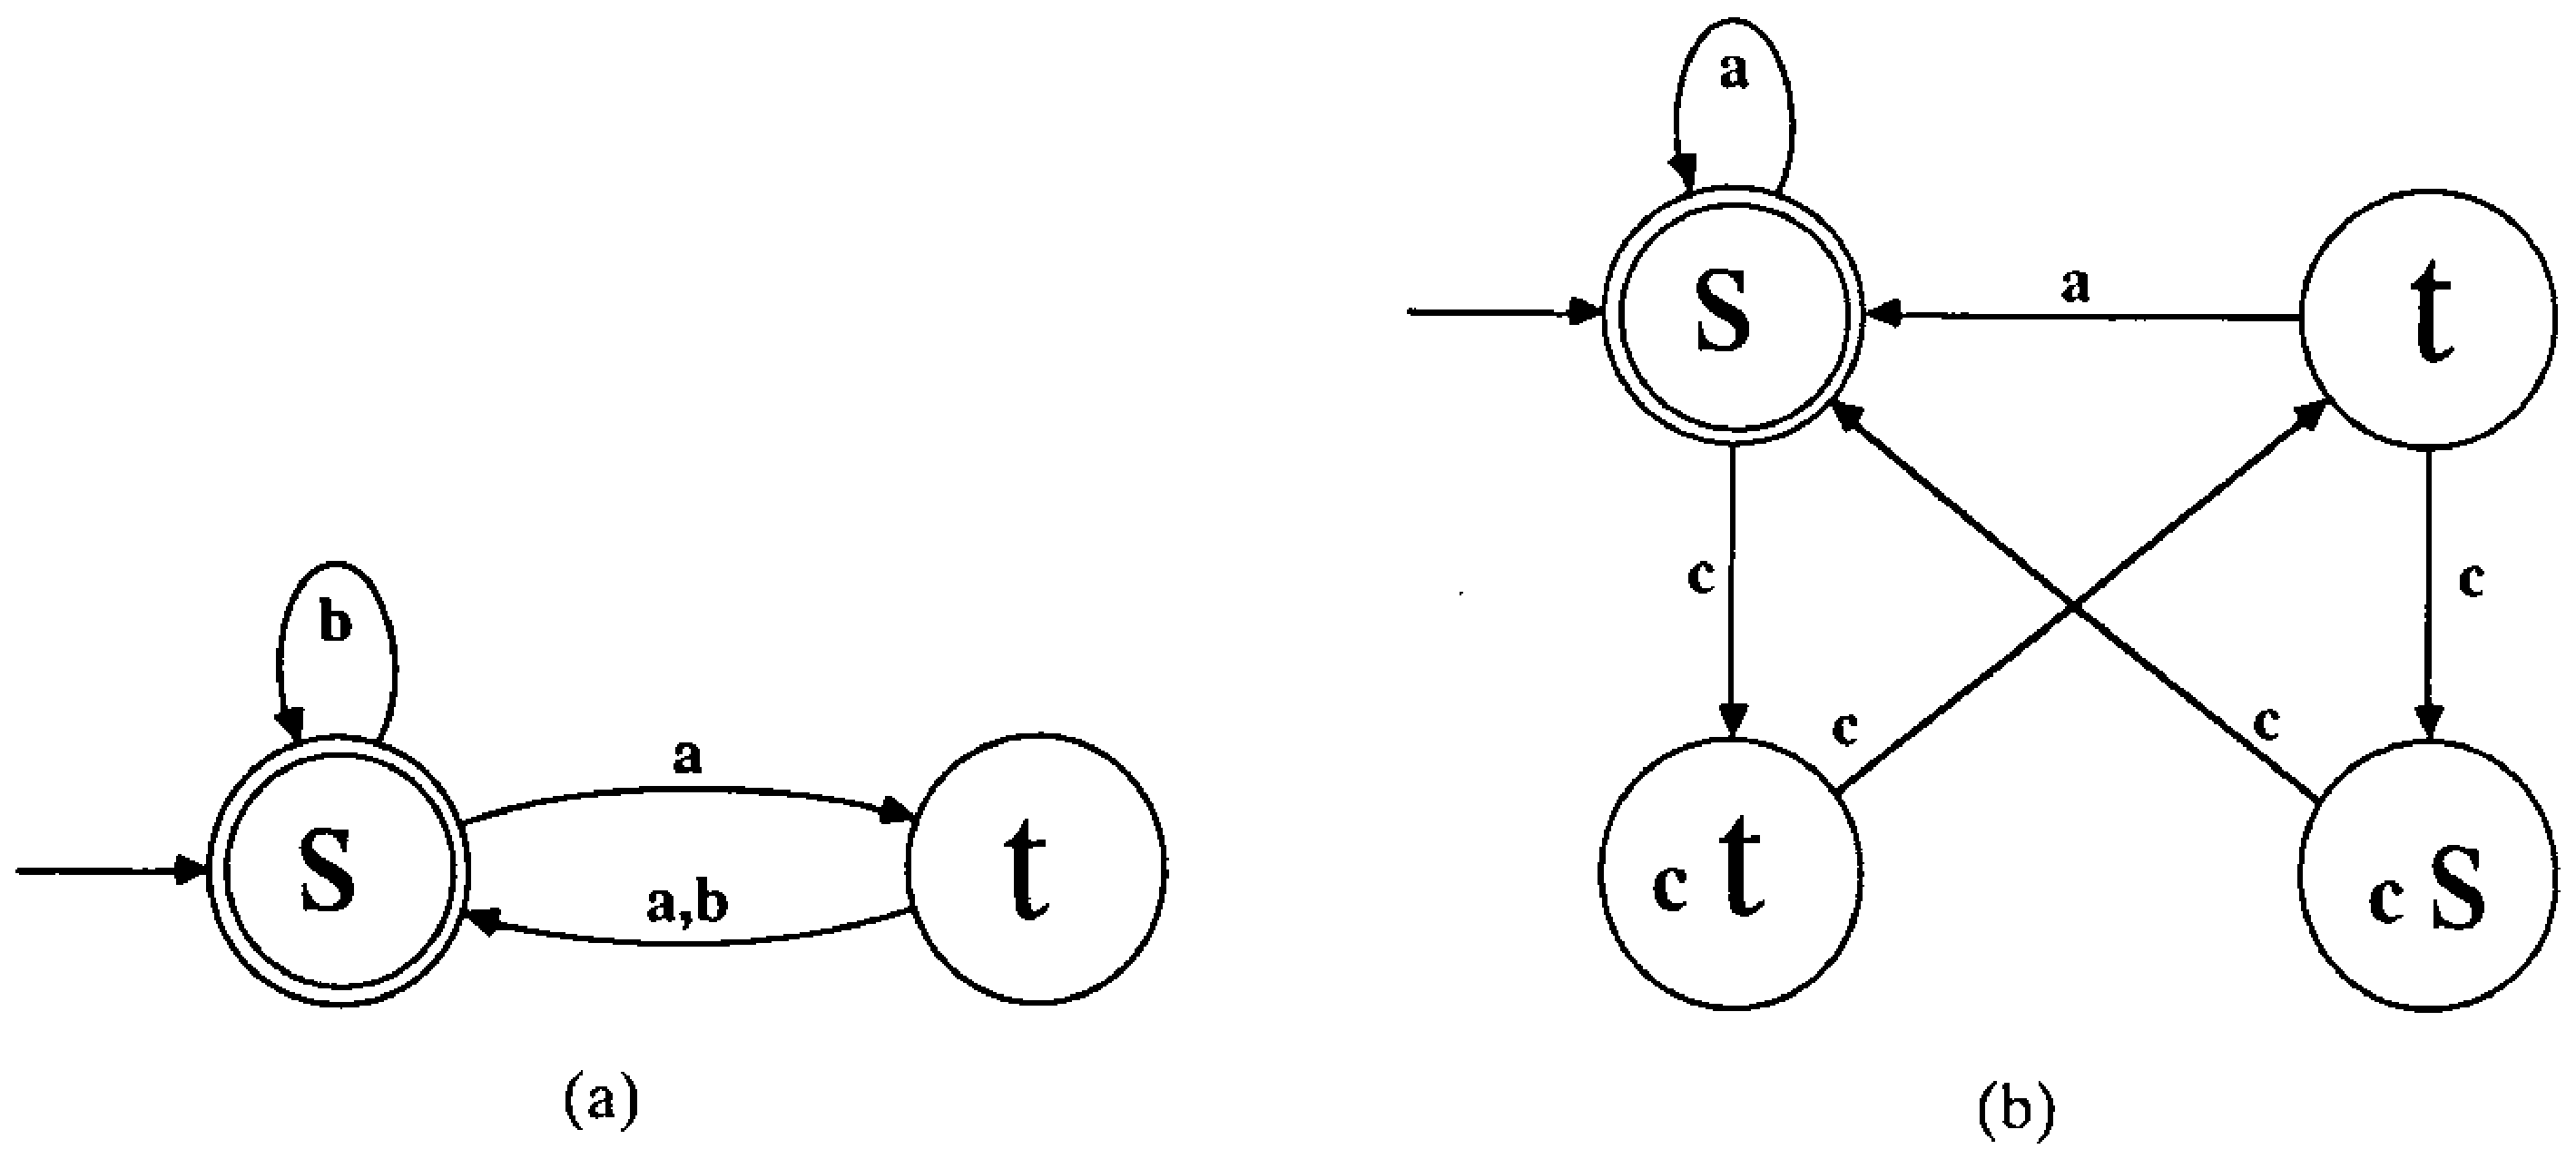
\epsfig{figure=ToFAfigures/fig5-20.eps,width=5.5in}}
\caption{(a) The automaton discussed in Example 5.22; (b) The resulting automaton
for Example 5.22}\label{fig-5.20}
\end{figure}

\subsection*{Example 5.23}

Consider the \emph{identity} homomorphism $\mu$$: \Sigma\rightarrow\Sigma^*$
defined by $(\forall \pmb{a} \in \Sigma)(\mu(\pmb{a})=\pmb{a})$. Since
$\overline{\mu}(L)=L$, \emph{any} collection of languages, including \NSIG, is
clearly closed under this homomorphism. Unlike \DSIG, though, there are many
homomorphisms under which \NSIG\ is not closed.

% Lemma 5.4
\begin{lmm}\label{lmm-5.4}\index{closure!under language homomorphism}
Let $\Sigma=\{\pmb{a},\pmb{b}\}$, and let $\xi$$: \Sigma\rightarrow\Sigma^*$ be
defined by $\xi(\pmb{a})=\pmb{a}$ and $\xi(\pmb{b})=\pmb{a}$. Then \NSIG\ is \emph{not}
closed under $\overline{\xi}$.

\emph{Proof.} Consider the set $L$ of all strings that have the same number of
$\pmb{a}$s as $\pmb{b}$s. This language is in \NSIG, but $\overline{\xi}(L)$ is the
set of all even-length strings of $\pmb{a}$s, which is clearly not in \NSIG.
\end{lmm}

A rather trivial example involves the homomorphism defined by $\psi(a)=\lambda$
for every letter $\pmb{a} \in \Sigma$. Then for all languages $L$, whether or
not $L \in \NSIG,\ \PBAR(L)=\{\lambda\}$, which is definitely not in \NSIG.

% Definition 5.9
\begin{dfn}\label{dfn-5.9}
Let $\psi$$: \Sigma\rightarrow\Gamma^*$ be a language homomorphism and consider
$z \in\Gamma^*$, The \emph{\Index{inverse homomorphic image} of z under $\PBAR$}
is then
\[ \overline{\psi^{-1}}(z)=\{x \in \Sigma^*\ |\ \PBAR(x) = z\} \]
For a language $L \subseteq \Gamma^*$, the \emph{\Index{inverse homomorphic
image} of L under} $\PBAR$ is defined by
\[ \overline{\psi^{-1}}(L)=\{x \in \Sigma^*\ |\ \PBAR(x) \in L\} \]
\end{dfn}

Thus, $x \in \overline{\psi^{-1}}(L) \Leftrightarrow \PBAR(x) \in L$. While the image of a
string under a homomorphism is a single word, note that the inverse image of a
single string may be an entire set of words.

\subsection*{Example 5.24}

Consider $\overline{\xi}$ from Lemma \ref{lmm-5.4} in which $\xi$$: \Sigma \rightarrow
\Sigma^*$ was defined by $\xi(\pmb{a})=\pmb{a}$ and $\xi(\pmb{b})=\pmb{a}$. Let
$z=\pmb{aa}$. Since $\overline{\xi}(\pmb{bb})=\overline{\xi}(\pmb{ba}) =
\overline{\xi}(\pmb{ab})=\overline{\xi}(\pmb{aa})=\pmb{aa}$,
\[ \overline{\xi^{-1}}\!(\pmb{aa})=\{\pmb{bb},\pmb{ba},\pmb{ab},\pmb{aa}\}
\text{. Note that } \overline{\xi^{-1}}\!(\pmb{ba})=\emptyset. \]

For $L=\{x \in\{\pmb{a}\}^*|\ |x|\equiv 0\bmod{3}\},\ 
\overline{\xi^{-1}}\!(L)=\{x\in\{\pmb{a},\pmb{b}\}^*|\ |x|\equiv 0\bmod{3}\}$.
Note that this second set is definitely larger, since it also contains words
with $\pmb{b}$s in them.

It can be shown that \DSIG\ is closed under inverse homomorphism. The trick is to
make the state transition function of the new automaton \emph{simulate}, for a
given letter $\pmb{a}$, the action the old automaton would have taken for the
entire string $\psi(\pmb{a})$. As the following proof will illustrate, the only
change that need take place is in the $\delta$ function; the newly constructed
machine is even deterministic!

% Theorem 5.10
\begin{thm}\label{thm-5.10}\index{closure!under inverse homomorphism}
Let $\Sigma$ be an alphabet, and let $\psi$$: \Sigma \rightarrow \Sigma^*$ be a
language homomorphism. Then \DSIG\ is closed under $\overline{\psi^{-1}}$.

\emph{Proof.} Let $L \in \DSIG$. Then there exists a DFA
$A=\langle\Sigma,S,s_0,\delta,F\rangle$ such that $L(A)=L$. Define a new DFA
$A^\psi=\langle\Sigma,S^\psi,s_0^\psi,\delta^\psi,F^\psi\rangle$ by
\begin{center}
\begin{tabular}{c}
$S^\psi = S$ \\
$s_0^\psi = s_0$ \\
$F^\psi = F$
\end{tabular}
\end{center}
and $\delta^\psi$ is defined by
\[ \delta^\psi(s,\pmb{a})=\DBAR\!(s,\psi(\pmb{a}))\ 
		\forall s \in S, \forall \pmb{a} \in \Sigma \]
Induction can be used to show $\overline{\delta^\psi}\!\!(s,x)=\DBAR(s,\PBAR(x))\forall s \in S,
\forall x \in \Sigma^*$\!\!, and in particular $\overline{\delta^{\psi}}(s_0,x)=\DBAR(s_0,\PBAR(x))$
$\forall x \in \Sigma^*$\!\!. Hence $L(A^\psi)=\overline{\psi^{-1}}(L(A))$.
\end{thm}

This theorem makes it possible to extend the range of the pumping lemma (Theorem
\ref{thm-2.3}) to many otherwise unpleasant problems. The set $M$ given in Example 5.20
can easily be shown to violate Theorem \ref{thm-2.3} and is therefore not FAD. The set $K$
given in Example 5.20 is just as clearly not FAD, but this is quite tedious to
formally prove by the pumping lemma (the number of choices for $u$, $v$, and $w$
is prohibitively large to thoroughly cover). An argument might proceed as
follows: Assume $K$ were FAD. Then $M$, being the inverse homomorphic image of a
FAD language, must also be FAD. Since $M$ is known (by an easy pumping lemma
proof) to be definitely not FAD, the assumption that $K$ is FAD must be
incorrect. Thus, $K \in \NSIG$.

% Lemma 5.5
\begin{lmm}\label{lmm-5.5}\index{closure!under inverse homomorphism}
Let $\Sigma=\{\pmb{a},\pmb{b}\}$, and let $\xi$$: \Sigma\rightarrow\Sigma^*$ be
defined by $\xi(\pmb{a})=\pmb{a}$ and $\xi(\pmb{b})=\pmb{a}$. Then \NSIG\ is
\emph{not} closed under $\overline{\xi^{-1}}$.

\emph{Proof.} Consider the set $L$ of all strings that have the same number of
$\pmb{a}$s as $\pmb{b}$s. This language is in \NSIG\ but $\overline{\xi^{-1}}(L)$ is
$\{\lambda\}$, which is clearly not in \NSIG.
\end{lmm}

We close this chapter by considering two operators for which it is definitely
not convenient to modify the structure of an existing automaton to construct a
new automaton with which to demonstrate closure.

% Theorem 5.11
\begin{thm}\label{thm-5.11}
Let $\Sigma$ be an alphabet. Define the operator $b$ by
\[ L^b=\{x\ |\ \exists y \in \Sigma^* \ni (xy \in L \wedge |x| = |y|)\} \]
Then \DSIG\ is closed under the operator $b$.

\emph{Proof.} $L^b$ represents the first halves of all the words in $L$. For
example, if $K=\{\pmb{ad},\pmb{abaa},\pmb{ccccc}\}$, then
$K^b=\{\pmb{a},\pmb{ab}\}$. Assume that $L$ is FAD. Then there exists a DFA 
$A=\langle\Sigma,S,s_0,\delta,F\rangle$ that accepts $L$. The proof consists of
identifying those states $q$ that are ``midway'' between the start state and a
final state; specifically, we need to identify the set of \emph{strings} for
which $q$ is the midpoint. The previous closure results for union, intersection,
homomorphism, and inverse homomorphism will be used to construct the language
representing $L^b$. Define the \emph{\Index{length}} homomorphism
$\psi$$: \Sigma\rightarrow\{\pmb{1}\}^*$ by $\psi(\pmb{a})=\pmb{1}$ for all
$\pmb{a} \in \Sigma$. Note that $\PBAR$ effectively counts the number of letters in a
word:
\[ \PBAR(x) = \pmb{1}^{|x|} \]
The following argument can be applied to each state $q$ to determine the set of
strings that use it as a ``midway'' state.

Consider the initial set for $q$, $I(A,q)=\{x\ |\ \DBAR(s_0,x)=q\}$ and the
terminal set for $q$, $T(A,q)=\{x\ |\ \DBAR(q,x) \in F\}$. We are interested in
finding those words in $I(A,q)$ that are the same length as words in $T(A,q)$.
$\PBAR(I(A,q))$ represents strings of $\pmb{1}$s whose lengths are the same as
words in $I(A,q)$. A similar interpretation can be given for $\PBAR(T(A,q))$.
Therefore, $\PBAR(I(A,q)) \cap \PBAR(T(A,q))$ will reflect those lengths that
are common to both the initial set and the terminal set. The inverse image under
\PBAR\ for this set will then reflect only those strings in $\Sigma^*$ that are
of the correct length to reach $q$ from $s_0$. This set is
$\overline{\psi^{-1}}(\PBAR(I(A,q)) \cap \PBAR(T(A,q)))$. Not all strings of a given
length are likely to reach $q$, though, so this set must be intersected with
$I(A,q)$ to correctly describe those strings that are both of the proper length
and that reach $q$ from the start state. This set,
$I(A,q) \cap \overline{\psi^{-1}}(\PBAR(I(A,q)) \cap \PBAR(T(A,q)))$, is thus the first
halves of all words that have $q$ as their midpoint. This process can be
repeated for each of the (finite) number of states in the automaton $A$, and the
union of the resulting sets will form all the first halves of words that are
accepted by $A$; that is, the union will equal $L^b$.

Note that by moving the start state of $A$ and forming the automaton
$A^q=\langle\Sigma,S,q,\delta,F\rangle$, each of the initial sets $I(A,q)$ can
be shown to be FAD. Similarly, the automaton
$A_q=\langle\Sigma,S,s_0,\delta,\{q\}\rangle$ illustrates that each terminal set
$T(A,q)$ must be FAD, also. Since $L^b$ has now been shown to be formed from
these basic FAD sets by applying homomorphisms, intersections, inverse
homomorphisms, and unions, $L^b$ must be FAD since \DSIG\ is closed under each
of these types of operations.
\end{thm}

\subsection*{Example 5.25}

Consider the automaton $A$ displayed in Figure \ref{fig-5.21}. For the state highlighted
as $q$, the quantities discussed in Theorem \ref{thm-5.11} would be as follows:
\begin{center}
\begin{tabular}{rcl}
$I(A,q)$ & $=$ & $\{\pmb{abc},\pmb{abcabc},\pmb{abcabcabc},\pmb{abcabcabcabc},
	\ldots\}$ \\
$T(A,q)$ & $=$ & $\{\pmb{aa},\pmb{aaaa},\pmb{aaaaaa},\pmb{aaaaaaaa},\ldots\}$ \\
& $=$ & $\{\pmb{a}^2,\pmb{a}^4,\pmb{a}^6,\pmb{a}^8,\pmb{a}^{10},\pmb{a}^{12},
	\ldots\}$ \\
$\PBAR(I(A,q))$ & $=$ & $\{\pmb{1}^3,\pmb{1}^6,\pmb{1}^9,\pmb{1}^{12},
	\pmb{1}^{15}, \ldots \}$ \\
$\PBAR(T(A,q))$ & $=$ & $\{\pmb{1}^2, \pmb{1}^4,\pmb{1}^6,\pmb{1}^8,\pmb{1}^{10},
	\pmb{1}^{12}, \ldots \}$ \\
$\PBAR(I(A,q))\cap\PBAR(T(A,q))$ & $=$ & $\{\pmb{1}^6,\pmb{1}^{12},\pmb{1}^{18},
	\ldots\}=\{x\in\{\pmb{1}\}^+|\ \ |x|\equiv 0\bmod{6}\}$ \\
$\overline{\psi^{-1}}(\PBAR(I(A,q))\cap\PBAR(T(A,q)))$ & $=$ & $\{x\in\{\pmb{a},\pmb{b},
	\pmb{c}\}^+|\ \ |x| \equiv 0\bmod{6}\}$ \\
& $=$ & $\{\pmb{aaaaaa},\pmb{aaaaab},\pmb{aaaaac},\pmb{aaaaba},\pmb{aaaabb},
	\ldots \}$ \\
$I(A,q)\cap\overline{\psi^{-1}}(\PBAR(I(A,q))\cap\PBAR(T(A,q)))$ & $=$ & $\{\pmb{abcabc},
	\pmb{abcabcabcabc}, \ldots \}$
\end{tabular}
\end{center}

% Figure 5.21
\begin{figure}
\centerline{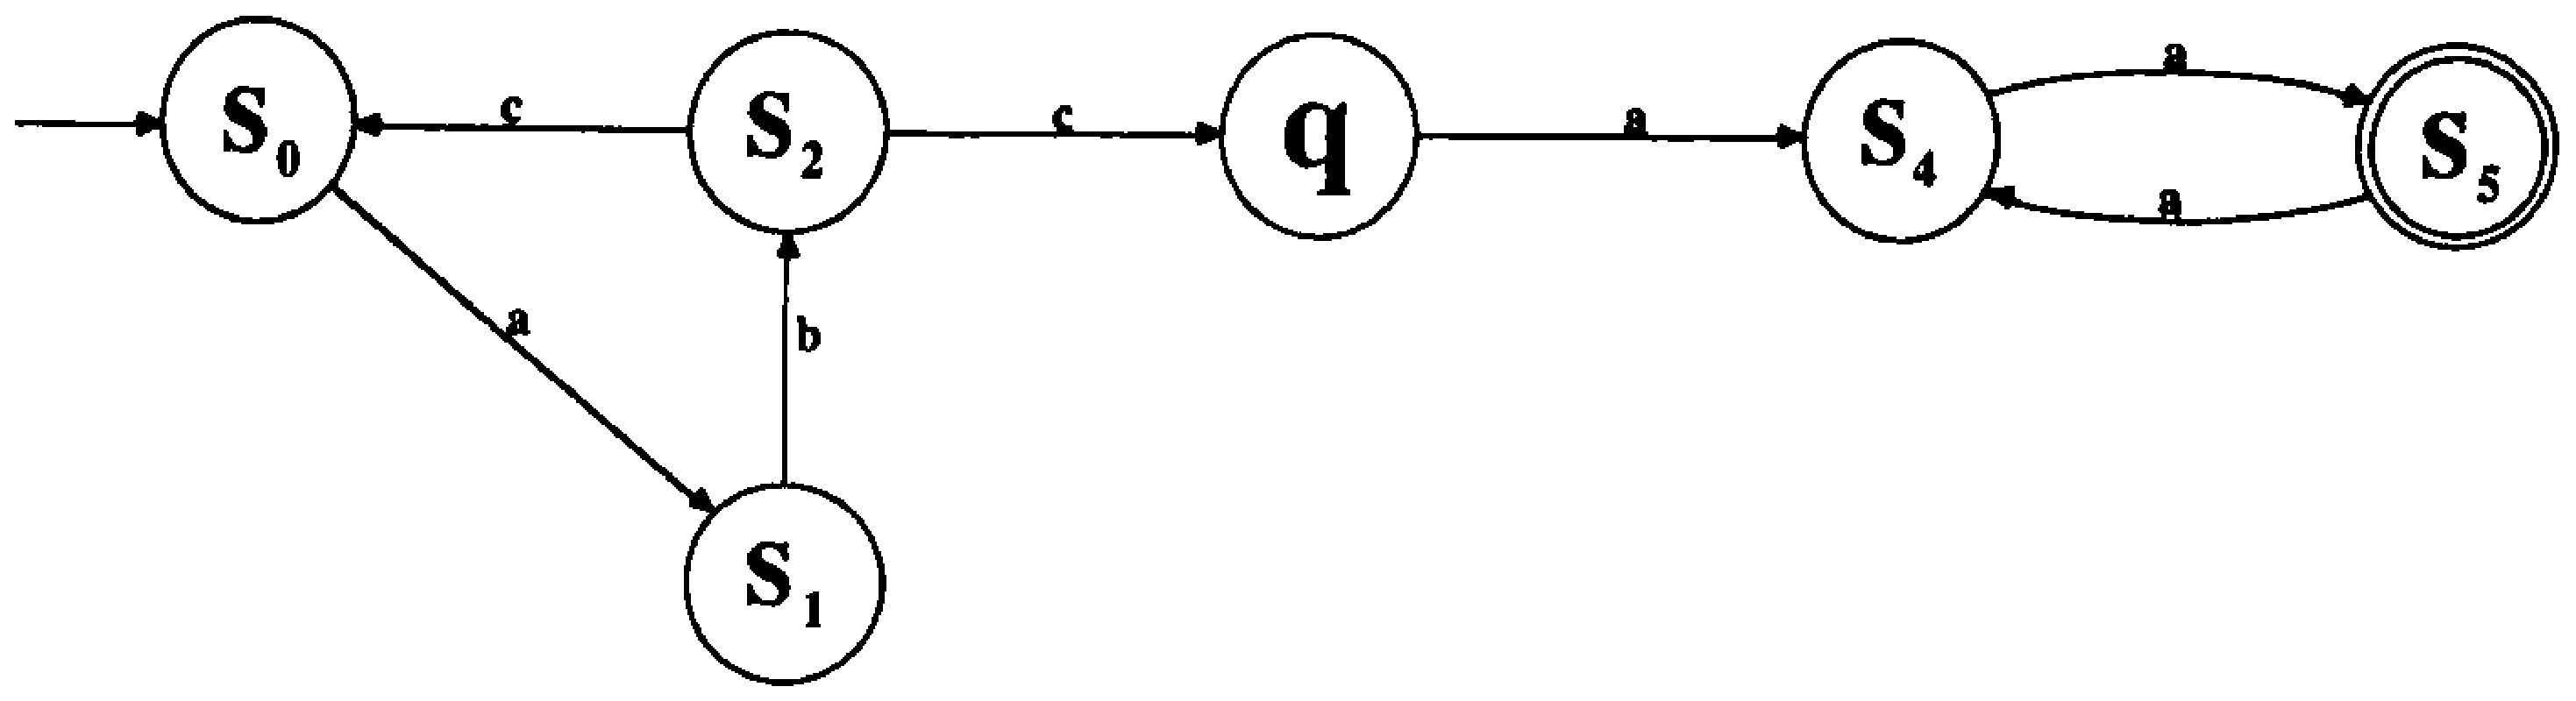
\epsfig{figure=ToFAfigures/fig5-21.eps,width=6in}}
\caption{The automaton discussed in Example 5.25}\label{fig-5.21}
\end{figure}

Similar calculations would have to be done for each of the other states of $A$.
Once again, \NSIG\ does not enjoy the same closure properties that \DSIG\ does.

% Lemma 5.6
\begin{lmm}\label{lmm-5.6}
Let $\Sigma = \{\pmb{a},\pmb{b}\}$.
Then \NSIG\ is not closed under the operator $b$.

\emph{Proof.} Let $L=\{\pmb{a}^n\pmb{b}^n$ $|$ $n \geq 0\}\in \NSIG$. Then $L^b=\{\pmb{a}^n$ $|$ $n\geq 0\}
\notin \NSIG$.
\end{lmm}

Other examples that show \NSIG\ is not closed under the operator $b$ abound. If
$K=\{x\in\{\pmb{a},\pmb{b}\}^*$ $|$ $\ |x|_{\pmb{a}} = |x|_{\pmb{b}}\}$, then
$K^b=\{\pmb{a},\pmb{b}\}^*$. The last operator we will cover in this chapter is
useful for illustrating closures that may not be \emph{effective}, that is, for which
there may not exist an algorithm for constructing the desired entity.
}

% Definition 5.10
\begin{dfn}\label{dfn-5.10}
Let $L_1$ and $L_2$ be languages. The \emph{\Index{quotient}} of $L_1$ with
$L_2$, written $L_1/L_2$, is defined by $L_1/L_2 =\{x$ $|$ $\exists y \in \Sigma^* \ni
y \in L_2 \wedge xy \in L_1\}$
\end{dfn}

Roughly speaking, the quotient consists of the beginnings of those words in
$L_1$ that terminate in a word from $L_2$.

\subsection*{Example 5.26}

Let $\Sigma=\{\pmb{a},\pmb{b}\}$. Then $\{\pmb{b}^2,\pmb{b}^4,\pmb{b}^6,\pmb{b}^8,
\pmb{b}^{10},\pmb{b}^{12},\ldots\}/\{\pmb{b}\}=\{\pmb{b}^1,\pmb{b}^3,\pmb{b}^5,
\pmb{b}^7,\pmb{b}^9,\pmb{b}^{11},\ldots\}$.\\Note that %\linebreak[4]
$\{\pmb{b}^2, \pmb{b}^4, \pmb{b}^6, \pmb{b}^8, \pmb{b}^{10}, \pmb{b}^{12},
\ldots\}/\{\pmb{a}\} = \{\ \}$.

% Theorem 5.12
\begin{thm}\label{thm-5.12}\index{closure!under quotient}
For any alphabet $\Sigma$, \DSIG\ is closed under quotient.

\emph{Proof.} Let $L_1$ and $L_2$ belong to \DSIG. Then there is a
deterministic finite automaton
$A_1=\langle\Sigma,S_1,s_{0_1},\delta_1,F\rangle$ such that $L(A_1)=L_1$. An
automaton that accepts $L_1/L_2$ can be defined by
$A^/=\langle\Sigma,S_1,s_{0_1},\delta_1,F^/\rangle$, where $F^/$ is defined to
be the set of all states $t$ for which there is a word in $L_2$ that reaches a
final state from $t$. That is, $F^/=\{t$ $|$ $\exists y \in \Sigma^*\ni (y \in L_2
\wedge \delta_1(t,y) \in F)\}$. It can be shown that $A^/$ does indeed accept
$L_1/L_2$, and hence \DSIG\ is closed under quotient (see the exercises).
\end{thm}

Note that the above proof did not mention the automaton associated with the
second language $L_2$. Indeed, the definition given for $F^/$ is sufficient to
argue that the new automaton does recognize the quotient of the two languages.
It was not actually necessary to deal with an automaton for $L_2$ in order to
argue that there must exist a DFA that recognizes $L_1/L_2$. The proof of
Theorem \ref{thm-5.12} is thus an \emph{existence} proof, but does not indicate whether
\DSIG\ is \emph{effectively} closed under quotient. Indeed, Theorem \ref{thm-5.12}
actually proves that the quotient of a FAD language with \emph{any} other language
(including those in \NSIG) will always be FAD. However, if it is hard to
determine just which strings in the other language may have the properties we
need to define $F^/$; we may not really know which subset of states $F^/$ should
actually be [after all, we could hardly check the property $\DBAR_1(q,y)\in F$,
one string at a time, for each of an infinite number of strings $y$ in $L_2$ in
a finite amount of time]. Fortunately, it is not necessary to know $F^/$
exactly, since there are only a finite number of ways to choose a set of final
states in the automaton $A^/$, and the proof of Theorem \ref{thm-5.12} assures us that one
of those ways must be the correct one that admits the conclusion
$L(A^/)=L_1/L_2$.

It would, however, be quite convenient to know what $F^/$ actually is so that we
could construct the automaton that actually accepts the quotient; this seems
much more satisfying that just knowing that such a machine must exist! If $L_2$
is FAD, the existence of an automaton
$A_2=\langle\Sigma,S_2,s_{0_2},\delta_2,F_2\rangle$ for which $L(A_2)=L_2$ does
make it possible to calculate $F^/$ exactly (see the exercises). Thus, \DSIG\ is
effectively closed under quotient. In later chapters, languages that may make it
impossible to determine $F^/$ will be studied. We defer the details of such
problems until then.

% Lemma 5.7
\begin{lmm}\label{lmm-5.7}\index{closure!under quotient}
Let $\Sigma=\{\pmb{a},\pmb{b}\}$. \NSIG\ is \emph{not} closed under quotient.

\emph{Proof.} Consider the set $L$ of all strings that have a different number
of $\pmb{a}$s than $\pmb{b}$s. This language is in \NSIG, but $L/L=\Sigma^*$ (why?).
\end{lmm}

From the exercises it will become clear that \NSIG\ is not closed over most of
the usual (or unusual!) operators. Note that \DSIG\ is by contrast a very
special set, in that it appears to be closed over every reasonable unary and
binary operation that we might consider. The question of closure will again
arise as more complex classes of machines and languages are presented in later
chapters.

\section*{Exercises}

\begin{enumerate}[{5.}1. ]
\item Let $\Sigma$ be an alphabet. Define $F_\Sigma$ to be the collection of all
finite languages over $\Sigma$. Prove or give counterexamples to the following:
\begin{enumerate}
\item $\pmb{F_\Sigma}$ is closed under complementation.
\item $\pmb{F_\Sigma}$ is closed under union.
\item $\pmb{F_\Sigma}$ is closed under intersection.
\item $\pmb{F_\Sigma}$ is closed under concatenation.
\item $\pmb{F_\Sigma}$ is closed under Kleene closure.
\item $\pmb{F_\Sigma}$ is closed under relative complement.
\end{enumerate}

\item Let $\Sigma$ be an alphabet. Define $C_\Sigma$ to be the collection of all
 \emph{cofinite}\index{cofinite!collection $C_\Sigma$} languages over $\Sigma$ (a language is cofinite if it is the complement
of a finite language). Prove or give counterexamples to the following:
\begin{enumerate}
\item $\pmb{C_\Sigma}$ is closed under complementation.
\item $\pmb{C_\Sigma}$ is closed under union.
\item $\pmb{C_\Sigma}$ is closed under intersection.
\item $\pmb{C_\Sigma}$ is closed under concatenation.
\item $\pmb{C_\Sigma}$ is closed under Kleene closure.
\item $\pmb{C_\Sigma}$ is closed under relative complement.
\end{enumerate}

\item Let $\Sigma$ be an alphabet. Define $B_\Sigma = F_\Sigma \cup C_\Sigma$
(see Exercises 5.1 and 5.2). Prove or give counterexamples to the following:
\begin{enumerate}
\item $\pmb{B_\Sigma}$ is closed under complementation.
\item $\pmb{B_\Sigma}$ is closed under union.
\item $\pmb{B_\Sigma}$ is closed under intersection.
\item $\pmb{B_\Sigma}$ is closed under concatenation.
\item $\pmb{B_\Sigma}$ is closed under Kleene closure.
\item $\pmb{B_\Sigma}$ is closed under relative complement.
\end{enumerate}

\item Let $\Sigma$ be an alphabet. Define $I_\Sigma$ to be the collection of all
infinite languages over $\Sigma$. Note that $I_\Sigma=\wp(\Sigma^*)-F_\Sigma$
(see Exercise 5.1). Prove or give counterexamples to the following:
\begin{enumerate}
\item $\pmb{I_\Sigma}$ is closed under complementation.
\item $\pmb{I_\Sigma}$ is closed under union.
\item $\pmb{I_\Sigma}$ is closed under intersection.
\item $\pmb{I_\Sigma}$ is closed under concatenation.
\item $\pmb{I_\Sigma}$ is closed under Kleene closure.
\item $\pmb{I_\Sigma}$ is closed under relative complement.
\end{enumerate}

\item Let $\Sigma$ be an alphabet. Define $J_\Sigma$ to be the collection of all
languages over $\Sigma$ that have infinite complements. Note that
$J_\Sigma=\wp(\Sigma^*)-C_\Sigma$ (see Exercise 5.2). Prove or give
counterexamples to the following:
\begin{enumerate}
\item $\pmb{J_\Sigma}$ is closed under complementation.
\item $\pmb{J_\Sigma}$ is closed under union.
\item $\pmb{J_\Sigma}$ is closed under intersection.
\item $\pmb{J_\Sigma}$ is closed under concatenation.
\item $\pmb{J_\Sigma}$ is closed under Kleene closure.
\item $\pmb{J_\Sigma}$ is closed under relative complement.
\end{enumerate}

\item Define $\pmb{E}$ to be the collection of all
languages over $\{\pmb{a},\pmb{b}\}$ that contain the word $\pmb{abba}$. Prove or
give counterexamples to the following:
\begin{enumerate}
\item $\pmb{E}$ is closed under complementation.
\item $\pmb{E}$ is closed under union.
\item $\pmb{E}$ is closed under intersection.
\item $\pmb{E}$ is closed under concatenation.
\item $\pmb{E}$ is closed under Kleene closure.
\item $\pmb{E}$ is closed under relative complement.
\end{enumerate}

\item If a collection of languages is closed under intersection, does it have
to be closed under union? Prove or give a counter example.

\item If a collection of languages is closed under intersection and complement,
does it have to be closed under union? Prove or give a counterexample.

\item Show that if a collection of languages is closed under concatenation it
is not necessarily closed under Kleene closure.

\item Show that if a collection of languages is closed under Kleene closure it
is not necessarily closed under concatenation.

\item Show that if a collection of languages is closed under complementation it
is not necessarily closed under relative complement.

\item Give a finite set of numbers that is closed under $\sqrt{\ \ }$.

\item Give an infinite set of numbers that is closed under $\sqrt{\ \ }$.

\item Given deterministic machines $A_1$ and $A_2$, use the definition of
$A^\cup$ and Definition \ref{dfn-4.5} to describe an algorithm for building a
\emph{deterministic} automaton $A^U$ that will accept $L(A_1) \cup L(A_2)$.

% Can't find how to change symbol size for the "A^\cup"s in (c)
\item Given deterministic machines $A_1$ and $A_2$, and without relying on the
construction used in Theorem \ref{thm-5.2}:
\begin{enumerate}
\item Build a \emph{deterministic} automaton $A^u$ that will accept
$L(A_1) \cup L(A_2)$.
\item Prove that your construction behaves as advertised.
\item If \emph{no} minimization is performed in Exercise 5.14, how do the number of
states in $A^\cup$, $A^U$, and $A^u$ compare? (Assume $A_1$ has $n$ states
and $A_2$ has $m$ states, and give expressions based on these variables.)
\end{enumerate}

\item Let $\Sigma$ be an alphabet. Define the (unary) operator $P$ by
\[ P(L)=\{x\ |\  \exists y \in \Sigma^* \ni xy \in L\}\text{ (for any collection of
words $L$)} \]
$P(L)$ then represents all the \emph{prefixes} of words in $L$. For example, if
$K =\{\pmb{a},\pmb{bbc},\pmb{dd}\}$, then
$P(K)=\{\pmb{\lambda},\pmb{a},\pmb{b},\pmb{bb},\pmb{bbc},\pmb{d},\pmb{dd}\}$. Prove
that \DSIG\ is closed under the operator $P$.

\item Let $\Sigma$ be an alphabet. Define the (unary) operator $S$ by
\[ S(L)=\{x\ | \ \exists y \in \Sigma^* \ni yx \in L\}\text{ (for any collection of
words $L$)} \]
$S(L)$ then represents all the \emph{suffixes} of words in $L$. For example, if
$K=\{\pmb{a},\pmb{bbc},\pmb{dd}\}$, then
$S(K)=\{\pmb{\lambda},\pmb{a},\pmb{c},\pmb{bc},\pmb{bbc},\pmb{d},\pmb{dd}\}$.
\begin{enumerate}
\item Given an automaton accepting $L$, describe how to modify it to produce an
automaton accepting $S(L)$.
\item Prove that your construction behaves as advertised.
\item Argue that \DSIG\ is closed under the operator $S$.
\end{enumerate}

\item Let $\Sigma$ be an alphabet. Define the (unary) operator $C$ by
\[ C(L)=\{x\ | \ \exists y,z \in \Sigma^* \ni yxz \in L\}
	\text{ (for any collection of words $L$)} \]
$C(L)$ then represents all the \emph{centers} of words in $L$. For example, if
$K=\{\pmb{a},\pmb{bbc},\pmb{dd}\}$, then $C(K)=\{\pmb{\lambda},\pmb{a},\pmb{c},
\pmb{bc},\pmb{bbc},\pmb{b},\pmb{bb},\pmb{d},\pmb{dd}\}$.
\begin{enumerate}
\item Given an automaton accepting $L$, describe how to modify it to produce an
automaton accepting $C(L)$.
\item Prove that your construction behaves as advertised.
\item Argue that \DSIG\ is closed under the operator $C$.
\end{enumerate}

\item Let $\Sigma$ be an alphabet. Define the (unary) operator $F$ by
\[ F(L)=\{x\ \ | \ x \in L \wedge (\text{if }\exists y \in \Sigma^* \ni xy \in L,
	\text{then }y = \lambda)\} \]
$F(L)$ then represents all the words in $L$ that are \emph{not} the beginnings of
other words in $L$. For example, if $K=\{\pmb{ad},\pmb{ab},\pmb{abbad}\}$, then
$F(K)=\{\pmb{ad},\pmb{abbad}\}$. Prove that \DSIG\ is closed under the operator
$F$.

\item Let $\Sigma$ be an alphabet, and $x=a_1a_2 \ldots a_{n-1}a_n \in \Sigma^*$;
define $x^r =a_na_{n-1} \ldots a_2a_1$. For a language $L$ over $\Sigma$, define
$L^r=\{x^r$ $|$ $x \in L\}$. Note that the (unary) reversal operator $r$ is thus defined
by $L^r=\{a_na_{n-1} \ldots a_3a_2a_1\ |\ a_1a_2a_3 \ldots a_{n-1}a_n \in L\}$, and
$L^r$ therefore represents all the words in $L$ written backward. For example, if
$K=\{\pmb{\lambda},\pmb{ad},\pmb{bbc},\pmb{bbad}\}$, then
$K^r=\{\pmb{\lambda},\pmb{da},\pmb{cbb},\pmb{dabb}\}$.
\begin{enumerate}
\item Given an automaton accepting L, describe how to modify it to produce an
automaton accepting $L^r$.\index{closure!under reversal}
\item Prove that your construction behaves as advertised.
\item Argue that \DSIG\ is closed under the operator $r$.
\end{enumerate}

\item Let $\Sigma=\{\pmb{a},\pmb{b},\pmb{c},\pmb{d}\}$. Define the (unary)
operator $G$ by
\[ G(L)=\{\pmb{a}_n\pmb{a}_{n-1}\ldots \pmb{a}_3\pmb{a}_2\pmb{a}_1\pmb{a}_1\pmb{a}_2\pmb{a}_3\ldots \pmb{a}_{n-1}\pmb{a}_n\ |\ \pmb{a}_1\pmb{a}_2\pmb{a}_3\ldots
	\pmb{a}_{n-1}\pmb{a}_n \in L\} \]
\[ =\{w^r \cdot w\ |\ w \in L\} \]
(see the definition of $w^r$ in Exercise 5.20). As an example, if
$K=\{\pmb{\lambda},\pmb{ad},\pmb{bbc},\pmb{bbad}\}$, then
$G(K)=\{\pmb{\lambda},\pmb{daad},\pmb{cbbbbc},\pmb{dabbbbad}\}$.
\begin{enumerate}
\item Prove that \DSIG\ is \emph{not} closed under the operator $G$.
\item Prove that \NSIG\ is closed under the operator $G$ (perhaps make use of Theorem \ref{thm-5.11}).
\item Prove that \NSIG\ is not closed under the operator $b$ ($b$ is defined in Theorem \ref{thm-5.11}).
\end{enumerate}

\item Prove that \NSIG\ is closed under the operator $r$ (see Exercise 5.20).\index{closure!under reversal}

\item Prove that \NSIG\ is \emph{not} closed under the operator $P$ (see
Exercise 5.16).

\item Prove that \NSIG\ is \emph{not} closed under the operator $S$ (see
Exercise 5.17).

\item Prove that \NSIG\ is \emph{not} closed under the operator $C$ (see
Exercise 5.18).

\item Prove that \NSIG\ is \emph{not} closed under the operator $F$ (see
Exercise 5.19).

\item Consider the following alternate ``proof'' of Theorem \ref{thm-5.1}: Let $A$ be an
\underline NDFA and define $A^\sim$ as suggested in Theorem \ref{thm-5.1}. Give an example to show
that $L(A^\sim)$ might not be equal to $\sim\!\!L(A)$.

\item Complete the proof of Lemma \ref{lmm-5.7}.

\item Give an example of a collection of languages that is closed under union,
concatenation, and Kleene closure, but is not closed under intersection.

\item If a collection of languages is closed under union, does it have to be
closed under intersection? Prove or give a counterexample.

\item Refer to the construction in Theorem \ref{thm-5.4} and prove that
$L(A^\bullet) = L_1 \cdot L_2$. Warning! This involves a \emph{lot} of tedious details.

\item Refer to the construction in Theorem \ref{thm-5.5} and prove that
$L(A_*) = L^*$. Warning! This involves a \emph{lot} of tedious details.

\item Amplify the explanations for each of the equivalences in the proof of
Theorem \ref{thm-5.2}.

\item Given a DFA $A=\langle\Sigma,S,s_0,\delta,F\rangle$, define an NDFA that
will accept $L(A)^+$.

\item Given an NDFA $A=\langle\Sigma,S,S_0,\delta,F\rangle$, define an NDFA that
will accept $L(A)^+$.

\item If $L$ is FAD, is it necessarily true that all subsets of $L$ are FAD?
Prove or give a counterexample.

\item If $L \in \DSIG$, is it necessarily true that all supersets of $L$ are in
\DSIG? Prove or give a counterexample.

\item If $L \in \NSIG$, is it necessarily true that all subsets of $L$ are in
\NSIG? Prove or give a counterexample.

\item If $L \in \NSIG$, is it necessarily true that all supersets of $L$ are in
\NSIG? Prove or give a counterexample.

\item Explain the purpose of the new start state $q_0$ in the proof of Theorem
\ref{thm-5.5}.

\item Redesign the construction in the proof of Theorem \ref{thm-5.4}, making use of
$\lambda$-transitions where appropriate.

\item Redesign the construction in the proof of Theorem \ref{thm-5.5}, making use of
$\lambda$-transitions where appropriate. Do this in such a way as to make the
``extra'' start state $q_0$ unnecessary.

\item Redesign the construction in the proof of Theorem \ref{thm-5.4}, assuming that $A_1$
and $A_2$ are NDFAs.

\item Redesign the construction in the proof of Theorem \ref{thm-5.5}, assuming that $A$
is a DFA.

\item How does the right congruence generated by a language $L$ compare to the
right congruence generated by the complement of $L$? \emph{Hint:} It may be
helpful to consider the construction of $A^\sim$ given in Theorem \ref{thm-5.1} when $A$
is a minimal machine accepting $L$.

\item \begin{enumerate}
\item Give examples of languages $L_1$ and $L_2$ for which
$R_{(L_1 \cap L_2)} = R_{L_1} \cap R_{L_2}$ (see Definition \ref {dfn-2.2}).
\item Give examples of languages $L_1$ and $L_2$ for which
$R_{(L_1 \cap L_2)} \not= R_{L_1} \cap R_{L_2}$. \emph{Hint:} It may be helpful
to consider the construction of $A^\cap$ given in Lemma \ref{lmm-5.1} to direct your
thinking.
\end{enumerate}

\item Consider the following assertion: \DSIG\ is closed under \emph{relative
complement;} that is, if $L_1$ and $L_2$ are FAD, then $L_1 - L_2$ is also FAD.
\begin{enumerate}
\item Prove this by appealing to existing theorems.
\item Define an appropriate ``new'' machine.
\item Prove that the machine constructed in part (b) behaves as advertised.
\end{enumerate}

\item Define $\mathfrak{L}_\Sigma$ to be the set of all languages recognized by
NDFAs with $\lambda$-transitions. What sort of closure properties does
$\mathfrak{L}_\Sigma$ have? How does $\mathfrak{L}_\Sigma$ compare to \DSIG?

\item \begin{enumerate}
\item Give an example of a language $L$ for which $\lambda \in L^+$.
\item Give three examples of languages $L$ for which $L^+ = L$.
\end{enumerate}

\item Recall that $\delta^\cup$$: (S_1 \cup S_2) \times \Sigma \rightarrow
\wp(S_1 \cup S_2)$ was defined by
\[ \delta^\cup(s,\pmb{a}) = \left\{\begin{tabular}{lrl}
	$\delta_1(s,\pmb{a})$ & if $s \in S_1$ & \\
	& , & $\forall s \in S_1 \cup S_2,\quad \forall\pmb{a} \in \Sigma$ \\
	$\delta_2(s,\pmb{a})$ & if $s \in S_2$ &
	\end{tabular}\right. \]
\begin{enumerate}
\item Prove (by induction) that $\overline{\delta^\cup}$ conforms to a similar formula:
\[ \overline{\delta^\cup}(s,x) = \left\{\begin{tabular}{lrl}
	$\DBAR_1(s,x)$ & if $s \in S_1$ & \\
	& , & $\forall s \in S_1 \cup S_2,\quad \forall x \in \Sigma^*$ \\
	$\DBAR_2(s,x)$ & if $s \in S_2$ &
	\end{tabular}\right. \]
\item Was this fact used in the proof of Theorem \ref{thm-5.2}?
\end{enumerate}

\item Let $\Sigma$ be an alphabet. Prove or give counterexamples to the
following:
\begin{enumerate}
\item \NSIG\ is closed under relative complement.
\item \NSIG\ is closed under union.
\item \NSIG\ is closed under concatenation.
\item \NSIG\ is closed under Kleene closure.
\item If $L \in \NSIG$, then $L^+ \in \NSIG$.
\end{enumerate}

\item Why was it necessary to require that $S_1 \cap S_2 = \emptyset$ in the
proof of Theorem \ref{thm-5.4}? Would any step of the proof be invalid without this
assumption? Explain.

\item Let $\Sigma$ be an alphabet. Define $E(L)=\{z\ |\ (\exists y \in \Sigma^+)
	(\exists x \in L)(z = yx)\}$.
\begin{enumerate}
\item Given an automaton accepting $L$, describe how to modify it to produce an
automaton accepting $E(L)$.
\item Prove that your construction behaves as advertised.
\item Argue that \DSIG\ is closed under the operator $E$.
\end{enumerate}

\item Let $\Sigma$ be an alphabet. Define
$B(L)=\{z\ $ $|$ $(\exists x\in L)(\exists y \in \Sigma^*)(z = xy)\}$.
\begin{enumerate}
\item Given an automaton accepting $L$, describe how to modify it to produce an
automaton accepting $B(L)$.
\item Prove that your construction behaves as advertised.
\item Argue that \DSIG\ is closed under the operator $B$.
\end{enumerate}

\item Let $\Sigma$ be an alphabet. Define
$M(L)=\{z\ $ $|$ $(\exists x \in L)(\exists y \in \Sigma^+)(z = xy)\}$.
\begin{enumerate}
\item Given an automaton accepting $L$. describe how to modify it to produce an
automaton accepting $M(L)$.
\item Prove that your construction behaves as advertised.
\item Argue that \DSIG\ is closed under the operator $M$.
\end{enumerate}

\item Refer to the definitions given in Lemma \ref{lmm-5.1} and use induction to show
that
\[ (\forall s \in S_1)(\forall t \in S_2)(\forall x \in \Sigma^*)(\overline{\delta^\cap}
	(\langle s,t\rangle,x) = \langle\DBAR_1(s,x),\DBAR_2(t,x)\rangle ) \]

\item Refer to Lemma \ref{lmm-5.1} and prove that $L(A^\cap)=L_1 \cap L_2$. As long as the
reference is explicitly stated, the result in Exercise 5.56 can be used without
proof.

\item Prove Theorem \ref{thm-5.6}.

\item Prove Theorem \ref{thm-5.7}.

\item \begin{enumerate}
\item Cleverly define a machine modification that does not use any
$\lambda$-moves that could be used to prove Theorem \ref{thm-5.7} (your new machine is
still likely to be nondeterministic, however).
\item Prove that your modified machine behaves as advertised.
\end{enumerate}

\item Let $W(L)=\{x\ $ $|$ $x$ is formed by deleting one or more letters from a word
in L$\}$.
\begin{enumerate}
\item Given an automaton accepting $L$, describe how to modify it to produce an
automaton accepting $W(L)$.
\item Prove that your construction behaves as advertised.
\item Argue that \DSIG\ is closed under the operator $W$.
\end{enumerate}

\item Let $V(L)=\{x $ $|$ $x$ is formed by deleting the odd-positioned letters from a
word in $L\}$. [\emph{Note:} This refers to the first, third, fifth, and so on,
letters in a word. For example, if $\pmb{abcdefg}\in L$, then $\pmb{bdf}\in
V(L)$.]
\begin{enumerate}
\item Given an automaton accepting $L$, describe how to modify it to produce an
automaton accepting $V(L)$.
\item Prove that your construction behaves as advertised.
\item Argue that \DSIG\ is closed under the operator $V$.
\end{enumerate}

\item Let $U(L)=\{x\ $ $|$ $x$ is formed by deleting the even-positioned letters from
a word in $L\}$. [\emph{Note:} This refers to the second, fourth, sixth, and so
on, letters in a word. For example, if $\pmb{abcdefg} \in L$, then
$\pmb{aceg} \in U(L)$.]
\begin{enumerate}
\item Given an automaton accepting $L$, describe how to modify it to produce an
automaton accepting $U(L)$.
\item Prove that your construction behaves as advertised.
\item Argue that \DSIG\ is closed under the operator U.
\end{enumerate}

\item Let $T(L)=\{x\ $ $|$ $x$ is formed by deleting every third, sixth, ninth, and so
on, letters from a word in $L\}$. [\emph{Note:} This refers to those letters in
a word whose index position is congruent to $0 \bmod{3}$. For example, if
$\pmb{abcdefg} \in L$, then $\pmb{abdeg} \in T(L)$.]
\begin{enumerate}
\item Given an automaton accepting $L$, describe how to modify it to produce an
automaton accepting $T(L)$.
\item Prove that your construction behaves as advertised.
\item Argue that \DSIG\ is closed under the operator $T$.
\end{enumerate}

\item For any alphabet $\Sigma$,
let $P=\{x\in\Sigma^*$ $|$ $|x|$ is prime$\}$ and let $I(L)$ be defined by
$I(L) = L \cap P$.
\begin{enumerate}
\item Show that \DSIG\ is not closed under $I$.
\item Show that $F_\Sigma$ is closed under $I$ (see Exercise 5.1).
\item Prove or disprove: $C_\Sigma$ is closed under $I$ (see Exercise 5.2).
\item Prove or disprove: $B_\Sigma$ is closed under $I$ (see Exercise 5.3).
\item Prove or disprove: $I_\Sigma$ is closed under $I$ (see Exercise 5.4).
\item Prove or disprove: $J_\Sigma$ is closed under $I$ (see Exercise 5.5).
\item Prove or disprove: $E$ is closed under $I$ (see Exercise 5.6).
\item Prove or disprove: \NSIG\ is closed under $I$.
\end{enumerate}

\item Define $C$ to be the collection of all languages over
$\{\pmb{a},\pmb{b}\}$ that do not contain $\lambda$. Prove or give
counterexamples to the following:
\begin{enumerate}
\item $C$ is closed under complementation.
\item $C$ is closed under union.
\item $C$ is closed under intersection.
\item $C$ is closed under concatenation.
\item $C$ is closed under Kleene closure.
\item $C$ is closed under relative complement.
\item If $L \in C$, then $L^+ \in C$
\end{enumerate}

\item \begin{enumerate}
\item Consider the statement that \DSIG\ is closed under finite union:
\begin{enumerate}
\item Prove by existing theorems and induction.
\item Prove by construction.
\end{enumerate}
\item Prove or disprove that \DSIG\ is closed under infinite union. Justify your
assertions.
\end{enumerate}

\item Let $\Sigma =\{\pmb{a},\pmb{b}\}$.
\begin{enumerate}
\item Give examples of three homomorphisms under which \NSIG\ is not closed.
\item Give examples of three homomorphisms under which \NSIG\ is closed.
\end{enumerate}

\item Let $\Sigma =\{\pmb{a}\}$. Can you find two different homomorphisms under
which \NSIG\ is not closed? Justify your conclusions.

\item Refer to the construction given in Theorem \ref{thm-5.10}.
\begin{enumerate}
\item Prove $\overline{\delta^{\psi}}\!(s,x)=\DBAR(s,\PBAR(x)) \forall s \in S,\forall x \in
	\Sigma^*$
\item Complete the proof of Theorem \ref{thm-5.10}.
\end{enumerate}

\item Consider the homomorphism $\xi$ given in Lemma \ref{lmm-5.4} and the set $L$ of all
strings that have the same number of $\pmb{a}$s as $\pmb{b}$s.
\begin{enumerate}
\item \DSIG\ is closed under inverse homomorphism, but $\xi(L)$ is the set of
all even-length strings of $\pmb{a}$s, and it appears that under
$\overline{\xi^{-1}}$ the DFA language $\xi(L)$ maps to the non-FAD language $L$.
Explain the apparent contradiction. \emph{Hint:} First compute
$\overline{\xi^{-1}}(\xi(L))$
\item Give an example of a homomorphism for which $\PBAR(\overline{\psi^{-1}}(L)) \not= L$.
\item Give an example of a homomorphism for which $\overline{\psi^{-1}}(\PBAR(L)) \not= L$.
\item Prove $\PBAR(\overline{\psi^{-1}}(L)) \subseteq L$.
\item Prove $L \subseteq \overline{\psi^{-1}}(\PBAR(L))$.
\end{enumerate}

\item Let $\Sigma$ be an alphabet. Define the (unary) operator $e$ by
\[ L^e=\{x\ | \ \exists y \in \Sigma^* \ni (yx \in L \wedge |x|=|y|)\} \]
$L^e$ then represents the last halves of all the words in $L$. For example, if
$K=\{\pmb{ad},\pmb{abaa},\pmb{ccccc}\}$, then $K^e=\{\pmb{d},\pmb{aa}\}$. Prove
that \DSIG\ is closed under the operator $e$.

\item Refer to the proof of Theorem \ref{thm-5.11} and show that there exists an automaton
$A$ for which it would be incorrect to try to accept $L^b$ by redefining the set
of final states to be merely the set of ``midway'' states.

\item Consider the sets $M$ and $K$ in Example 5.20. Assume that we have used
the pumping lemma to show that $M$ is not FAD. What would be wrong with arguing
that, since $M$ was not FAD, its homomorphic image cannot be FAD either, and
hence $K$ is therefore not FAD.

\item Prove Theorem \ref{thm-5.9}.

\item Let $\Sigma$ be the ASCII alphabet. Define a homomorphism that will
capitalize all lowercase letters (and does not change punctuation, spelling, and
the like).

\item Consider the proof of Theorem \ref{thm-5.12}.
\begin{enumerate}
\item Show that
$L(A^{^/}) = L_1/L_2$
for the $A$ and $A^{^/}$ defined by
$A=\langle\Sigma,S_1,s_{0_1},\delta_1,F\rangle$ and
$A^{^/}=\langle\Sigma,S_1,s_{0_1},\delta_1,F{^/}\rangle$, where
$ F^{^/} =\{t\ | \ \exists y \in \Sigma^* \ni (y \in L_2 \wedge \DBAR_1(t,y) \in F)\}$.
\item Given deterministic finite automata
$A_1=\langle\Sigma,S_1,s_{0_1},\delta_1,F\rangle$ such that $L(A_1) = L_1$,
and $A_2=\langle\Sigma,S_2,s_{0_2},\delta_2,F_2\rangle$ for which $L(A_2) = L_2$,
give an algorithm for computing $F^{^/}=\{t$ $|$ $\exists y \in \Sigma^* \ni (y \in L_2
\wedge \DBAR_1(t,y) \in F)\}$.
\end{enumerate}

\item Given two alphabets $\Sigma_1$ and $\Sigma_2$ and a DFA
$A=\langle\Sigma_1,S,s_0,\delta,F\rangle$:
\begin{enumerate}
\item Define a new automaton $A'=\langle\Sigma_1 \cup \Sigma_2,S',s_0',\delta',
F'\rangle$ for which $L(A')=L(A)$.
\item Prove that $A'$ behaves as advertised.
\end{enumerate}

\item Let $S$ be a collection of languages that is closed under union,
concatenation, and Kleene closure. Prove or disprove: If $S$ contains an
infinite number of languages, every language in $S$ must be FAD.

\item Let $S$ be a collection of languages that is closed under union,
concatenation, and Kleene closure. Prove or disprove: If $S$ is a finite
collection, every language in $S$ must be FAD.

\item Let $u$ be a unary language operator that, when composed with itself,
yields the identity function. Prove that if \DSIG\ is closed under $u$,
then \NSIG\ must also be closed under $u$.
\end{enumerate}

% Chapter, Section, Figure, Table, Theorem, Corollary, Lemma, Definition, {\bf  
\chapter{Regular Expressions}\label{ch-6}

In this chapter we will develop a standard notation for denoting FAD languages
and thus explore yet another characterization of these languages. The
specification of a language by an automaton unfortunately does not provide a
convenient summary of those strings that are accepted; it is straightforward to
check whether any particular word belongs to the language, but it is often
difficult to get an overall sense of the set of accepted words. Were the
language finite, the individual words could simply be explicitly listed. The
delineation of an infinite set in this manner is clearly impossible.

Up to this point, we have relied on English descriptions of the languages under
consideration. Natural languages are unfortunately imprecise, and even small
machines can have impossibly complex descriptions. The concept of regular
expressions provides a clear and concise vehicle for denoting many of the
languages we have studied in the previous chapters.

\section{Algebra of Regular Expressions}\label{sec-6.1}

The definition of set union and the concepts of language concatenation
(Definition \ref{dfn-5.4}) and \Index{Kleene closure} (Definition \ref{dfn-5.5}) afford a convenient and
powerful method for building new languages from existing ones. The expression
$(\{\pmb{a},\pmb{b}\}\cdot\{\pmb{c}\})^*\cdot\{\pmb{d}\}$ is an infinite set
built from simple alphabets and the operators presented in Chapter \ref{ch-5}. We will
see that this type of representation is quite suitable for our purposes and is
intimately related to the finite automaton definable languages.

% Definition 6.1
\begin{dfn}\label{dfn-6.1}
Let $\Sigma =\{\pmb{a}_1,\pmb{a}_2, \ldots ,\pmb{a}_m\}$ be an alphabet. A
\emph{\Index{regular set over $\Sigma$}} is any set that can be formed by a
sequence of applications of the following rules:
\begin{enumerate}[i.]
\item $\{\pmb{a}_1\},\{\pmb{a}_2\}, \ldots ,\{\pmb{a}_m\}$ are regular sets.
\item $\{\ \}$ (the empty set of words) is a regular set.
\item $\{\lambda\}$ (the set containing only the empty \emph{word}) is a regular set.
\item If $L_1$ and $L_2$ are regular sets, then so is $L_1 \cdot L_2$.
\item If $L_1$ and $L_2$ are regular sets, then so is $L_1 \cup L_2$.
\item If $L_1$ is a regular set, then so is $L_1^*$.
\end{enumerate}
\end{dfn}
\subsection*{Example 6.1}

Let $\Sigma = \{\pmb{a},\pmb{b},\pmb{c}\}$. Each of the following languages are
regular sets:
\begin{center}\begin{tabular}{llll}
$\{\lambda\}$ & $\{\pmb{b}\}\cup\{\pmb{c}\}$ & $\{\pmb{a}\}\cdot(\{\pmb{b}\}\cup
	\{\pmb{c}\})$ & $\{\pmb{b}\cdot\lambda\}$ \\
$\{\pmb{a}\}^*$ & $(\{\pmb{a}\}\cup\{\lambda\})\cdot(\{\pmb{b}\}^*)$ & $\{\ \}^*$
	& $\{\pmb{c}\}\cdot\{\ \}$
\end{tabular}\end{center}

The multitude of set brackets in these expressions is somewhat undesirable;
we now present a common shorthand notation to represent such sets. Expressions
like $\{\pmb{a}\}^*$ will simply be written as $\pmb{a}^*$, and $\{\pmb{a}\}
\cdot \{\pmb{b}\}$ will be shortened to $\pmb{ab}$. The notation we wish to use
can be formally defined in the following recursive manner.

% Definition 6.2
\begin{dfn}\label{dfn-6.2}
Let $\Sigma=\{\pmb{a}_1,\pmb{a}_2, \ldots ,\pmb{a}_m\}$ be an alphabet. A
\emph{\Index{regular expression} over} $\Sigma$ is a sequence of symbols formed
by repeated application of the following rules:
\begin{enumerate}[i.]
\item $\pmb{a}_1,\pmb{a}_2, \ldots ,\pmb{a}_m$ are all regular expressions,
	representing the regular sets $\{\pmb{a}_1\},\{\pmb{a}_2\}, \ldots ,
	\{\pmb{a}_m\}$, respectively.
\item $\emptyset$ is a regular expression representing $\{\ \}$.
\item $\epsilon$\index{e@$\epsilon$ (regular expression)} is a regular expression representing $\{\lambda\}$.
\item If $R_1$ and $R_2$ are regular expressions corresponding to the sets $L_1$
	and $L_2$, then $(R_1 \cdot R_2)$ is a regular expression representing
	the set $L_1 \cdot L_2$.
\item If $R_1$ and $R_2$ are regular expressions corresponding to the sets $L_1$
	and $L_2$, then $(R_1 \cup R_2)$ is a regular expression representing
	the set $L_1 \cup L_2$.
\item If $R_1$ is a regular expression corresponding to the set $L_1$, then
	$(R_1)^*$ is a regular expression representing the set $L_1^*$.
\end{enumerate}
\end{dfn}

\subsection*{Example 6.2}

Let $\Sigma=\{\pmb{a},\pmb{b},\pmb{c}\}$. The regular sets in Example 6.1 can be
represented by the following regular expressions:
\begin{center}\begin{tabular}{llll}
$\epsilon$ & $(\pmb{b}\cup\pmb{c})$ & $(\pmb{a}\cdot(\pmb{b}\cup\pmb{c}))$ &
	$(\pmb{b} \cdot \epsilon)$ \\
$(\pmb{a})^*$ & $((\pmb{a}\cup\epsilon)\cdot(\pmb{b})^*)$ & $(\emptyset)^*$ &
	$(\pmb{c}\cdot\emptyset)$
\end{tabular}\end{center}
Note that each expression consists of the ``basic building blocks'' given by
6.2i through 6.2iii and are connected by the operators $\cup$, $\cdot$ and $^*$
according to rules 6.2iv through 6.2vi. Each expression is intended to denote a
particular language over $\Sigma$. Such representations of languages are by no
means unique. For example, $(\pmb{a}\cdot(\pmb{b}\cup\pmb{c}))$ and $((\pmb{a}
\cdot\pmb{b})\cup(\pmb{a}\cdot\pmb{c}))$ both represent the same set,
$\{\pmb{ab},\pmb{ac}\}$. Similarly, $(\pmb{b}\cdot\epsilon)$ and $\pmb{b}$ both
represent $\{\pmb{b}\}$.

The intention of the parentheses is to prevent ambiguity; $\pmb{a}\cdot\pmb{b}
\cup\pmb{c}$ could mean $(\pmb{a}\cdot(\pmb{b}\cup\pmb{c}))$ or $((\pmb{a}\cdot
\pmb{b})\cup\pmb{c})$, and the difference is important: the first expression
represents $\{\pmb{ab},\pmb{ac}\}$, while the second represents $\{\pmb{ab},
\pmb{c}\}$, which are obviously different languages. To ease the burden of all
these parentheses, we will adopt the following simplifying conventions.

{\bf Notational Convention}: The precedence of the operators, from highest to
lowest, shall be $^*$, $\cdot$, $\cup$. When writing a regular expression,
parentheses that conform to this hierarchy may be omitted. In particular, the
outermost set of parentheses can always be omitted. Juxtaposition may be used in
place of the concatenation symbol $(\cdot)$.

\subsection*{Example 6.3}

Thus, $\pmb{a}\cdot\pmb{b}\cup\pmb{c}$ will be taken to mean $((\pmb{a}\cdot
\pmb{b})\cup\pmb{c})$, not $(\pmb{a}\cdot(\pmb{b}\cup\pmb{c}))$, since $\cdot$
has precedence over $\cup$. Redundant parentheses that are implied by the
precedence rules can be eliminated, and thus $(((\pmb{a}\cdot\pmb{b})\cup\pmb{c})
\cdot\pmb{d})$ can be written as $(\pmb{ab}\cup\pmb{c})\pmb{d}$. Notice that
$\pmb{b}\cup\pmb{c}^*$ represents $(\pmb{b}\cup(\pmb{c}^*))$, not $(\pmb{b}\cup
\pmb{c})^*$. Kleene closure therefore behaves much like exponentiation does in
ordinary algebraic expressions in that it is given precedence over the other
operators. Concatenation and union behave much like the algebraic operators
multiplication and addition, respectively. Indeed, some texts use $+$ instead of
$\cup$ for union; the symbol for concatenation already agrees with that for
multiplication $(\cdot)$, and we will likewise allow the symbol to be omitted
in favor of juxtaposition. The constants $\emptyset$ and $\epsilon$ behave much
like the numbers $\pmb{0}$ and $\pmb{1}$ do in algebra. The common identities
$x+0=x,\ x\cdot 1=x$ and $x\cdot 0=0$ have parallels in language theory (see
Lemma \ref{lmm-6.1}). In particular,
$\emptyset$ is the \emph{identity} for union and $\epsilon$
is the identity for concatenation.

Thus far we have been very careful to distinguish between the name of an object
and the object itself. In algebra, we are used to saying that the symbol
$\pmb{4}$ \emph{equals} the string of symbols (that is, the word) $20 \div 5$; we
really mean that both names refer to the same object, the concept we generally
call the number \emph{four}. (You should be able to think of many more strings
that are commonly used as a name for this number, for example, $||||$, IV, and
$100_2$). We will be equally inexact here, writing $\pmb{a}\cdot(\pmb{b}\cup
\pmb{c})=(\pmb{a}\cdot\pmb{b})\cup(\pmb{a}\cdot\pmb{c})$. This will be taken to
mean that the \emph{sets represented} by the two expressions are equal (as is
the case here; both equal $\{\pmb{ab},\pmb{ac}\}$) and will not be construed to
mean that the two \emph{expressions themselves} are identical (which is clearly
not the case here; the right-hand side has more $\pmb{a}$s, more parentheses, and
more concatenation symbols).

% Definition 6.3
\begin{dfn}\label{dfn-6.3}\index{equivalent!regular expressions}
Let $R$ be a regular expression. The language represented by R is formally
denoted by $L(R)$. Two regular expressions $R_1$ and $R_2$ will be said to be
\emph{equivalent} if the sets represented by the two expressions are
equal, and we will write $R_1 = R_2$.
\end{dfn}

Thus, $R_1$ and $R_2$ are equivalent if $L(R_1) = L(R_2)$, but this is commonly
abbreviated $R_1 = R_2$. The word ``equivalent'' has been seen in three
different contexts so far: there are equivalent DFAs, equivalent NDFAs, and now
equivalent regular expressions. In each case, the intent has been to equate
constructs that are associated with the same language. Now that the idea of
equality (equivalence) has been established, some general identities can be
outlined. The properties given in Lemma \ref{lmm-6.1} follow directly from the definitions
of the operators.

% Lemma 6.1
\begin{lmm}\label{lmm-6.1}\index{associative law}\index{commutative law}
Let $\Sigma$ be an alphabet, and let $R_1,\ R_2$, and $R_3$ be regular
expressions. Then:
\begin{enumerate}[(a)]
\item $R_1 \cup \emptyset = R_1$
\item $R_1 \cdot \epsilon = R_1 = \epsilon \cdot R_1$
\item $R_1 \cdot \emptyset = \emptyset = \emptyset \cdot R_1$
\item $R_1 \cup R_2 = R_2 \cup R_1$
\item $R_1 \cup R_1 = R_1$
\item $R_1 \cup (R_2 \cup R_3) = (R_1 \cup R_2) \cup R_3$
\item $R_1 \cdot (R_2 \cdot R_3) = (R_1 \cdot R_2) \cdot R_3$
\item $R_1 \cdot (R_2 \cup R_3) = (R_1 \cdot R_2) \cup (R_1 \cdot R_3)$
\item $\epsilon^* = \epsilon$
\item $\emptyset^* = \epsilon$
\item $(R_1 \cup R_2)^* = (R^*_1 \cup R^*_2)^*$
\item $(R_1 \cup R_2)^* = (R^*_1 \cdot R^*_2)^*$
\item $(R^*_1)^* = R^*_1$
\item $(R_1)^* \cdot (R^*_1) = R^*_1$
\end{enumerate}
Furthermore, there are examples of sets for which: \\
\begin{tabular}{rl}
(b$'$) & $R_1 \cup \epsilon \not= R_1$ \\
(d$'$) & $R_1 \cdot R_2 \not= R_2 \cdot R_1$ \\
(e$'$) & $R_1 \cdot R_1 \not= R_1$ \\
(h$'$) & $R_1 \cup (R_2 \cdot R_3) \not= (R_1 \cup R_2) \cdot (R_1 \cup R_3)$ \\
(k$'$) & $(R_1 \cdot R_2)^* \not= (R^*_1 \cdot R^*_2)^*$ \\
(l$'$) & $(R_1 \cdot R_2)^* \not= (R^*_1 \cup R^*_2)^*$
\end{tabular}

\emph{Proof.} Property (h) will be proved here. The remainder are left as
exercises.

\begin{center}\begin{tabular}{rcl}
$w \in R_1 \cdot (R_2 \cup R_3)$ & $\Leftrightarrow$ & (by definition of
	$\cdot$) \\
$(\exists x,y)(y \in (R_2 \cup R_3) \wedge x \in R_1 \wedge w = x \cdot y)$ &
	$\Leftrightarrow$ & (by definition of $\cup$) \\
$(\exists x,y)((y \in R_2 \vee y \in R_3) \wedge (x \in R_1 \wedge w = x \cdot
	y))$ & $\Leftrightarrow$ & (by the distributive law) \\
$(\exists x,y)(((y \in R_2) \wedge (x \in R_1 \wedge w = x \cdot y))$ && \\
$\vee ((y \in R_3) \wedge (x \in R_1 \wedge w = x \cdot y)))$ & $\Leftrightarrow$ 
	& (by definition of $\cdot$) \\
$(\exists x,y)((w = x \cdot y \in R_1 \cdot R_2) \vee (w = x \cdot y \in R_1
	\cdot R_3))$ & $\Leftrightarrow$ & (by definition of $\cup$) \\
$w \in (R_1 \cdot R_2) \cup (R_1 \cdot R_3)$ &&
\end{tabular}\end{center}
\end{lmm}

Note that identity (c) in Lemma \ref{lmm-6.1} implies that $\{\pmb{a},\pmb{b}\}\cdot
\emptyset = \emptyset$, which follows immediately from the definition of
concatenation. If $w \in \{\pmb{a},\pmb{b}\} \cdot \emptyset$, then $w$ would
have to be of the form $x \cdot y$, where $x \in \{\pmb{a},\pmb{b}\}$ and
$y \in \emptyset$; there are clearly no valid choices for $y$, so $\{\pmb{a},
\pmb{b}\} \cdot \emptyset$ is empty.

\section{Regular Sets As FAD Languages}\label{sec-6.2}

Armed with the constructs and properties discussed in the first section, we will
now consider what types of languages can actually be defined by regular
expressions. How general is this method of expressing sets of words? Can the FAD
languages be represented by regular expressions? (Yes). Can all programming
languages be represented by regular expressions? (No). Are regular sets always
finite automaton definable languages? (Yes). We begin by addressing this last
question.

% Definition 6.4
\begin{dfn}\label{dfn-6.4}\index{R@\RSIG \ (R-sigma )}
Let $\Sigma$ be an alphabet. \RSIG\ is defined to be the set of all regular
sets over $\Sigma$.
\end{dfn}

The first question to be considered is, Can every regular set be recognized by
a DFA? That is, is $\RSIG$~$\subseteq$~$\DSIG$? It is clear that the ``basic
building blocks'' are recognizable. Figure \ref{fig-6.1} shows three
\underline{NDFA}s that accept
$\{\ \}$, $\{\lambda\}$, and $\{\pmb{c}\}$, respectively.\index{basic NDFAs} Recalling the
constructions outlined in Chapter \ref{ch-5}, it is easy to see how to combine these
``basic machines'' into machines that will accept expressions involving the
operators $\cup$, $\cdot$, and $^*$.

\subsection*{Example 6.4}

An NDFA that accepts $\pmb{a}\cup\pmb{b}$ (as suggested by the proof of Theorem
\ref{thm-5.2}) is shown in Figure \ref{fig-6.2}. Note that it is composed of the basic building
blocks for the letters $\pmb{a}$ and $\pmb{b}$, as suggested by the
constructions in Figure \ref{fig-6.1}. 

% Figure 6.1
\begin{figure}
\centerline{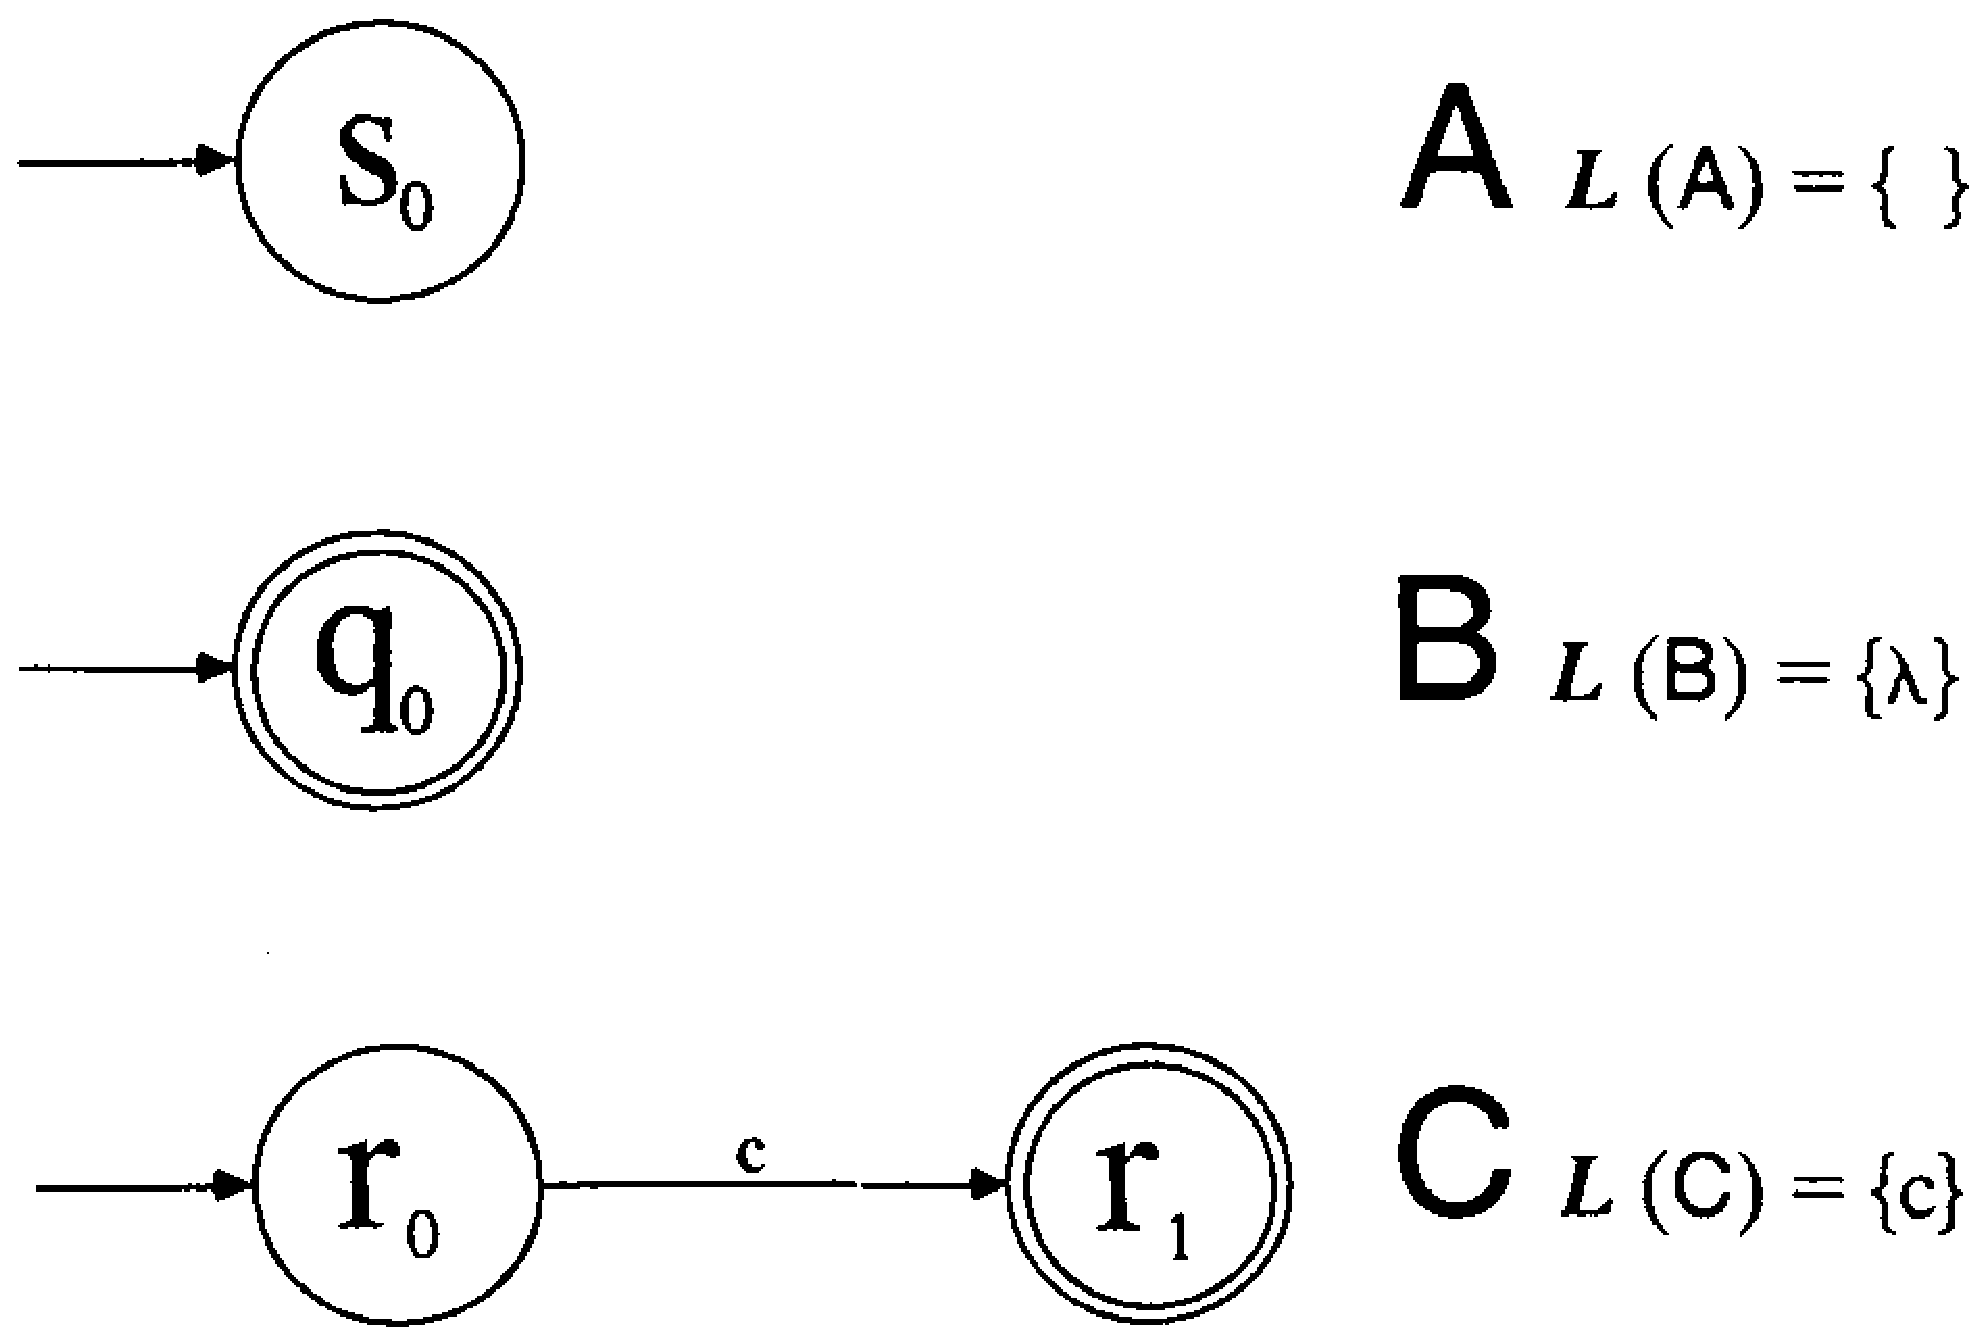
\epsfig{figure=ToFAfigures/fig6-1.eps,width=4in}}
\caption{NDFAs which recognize regular expressions with zero operators}\label{fig-6.1}
\end{figure}

% Figure 6.2
\begin{figure}
\centerline{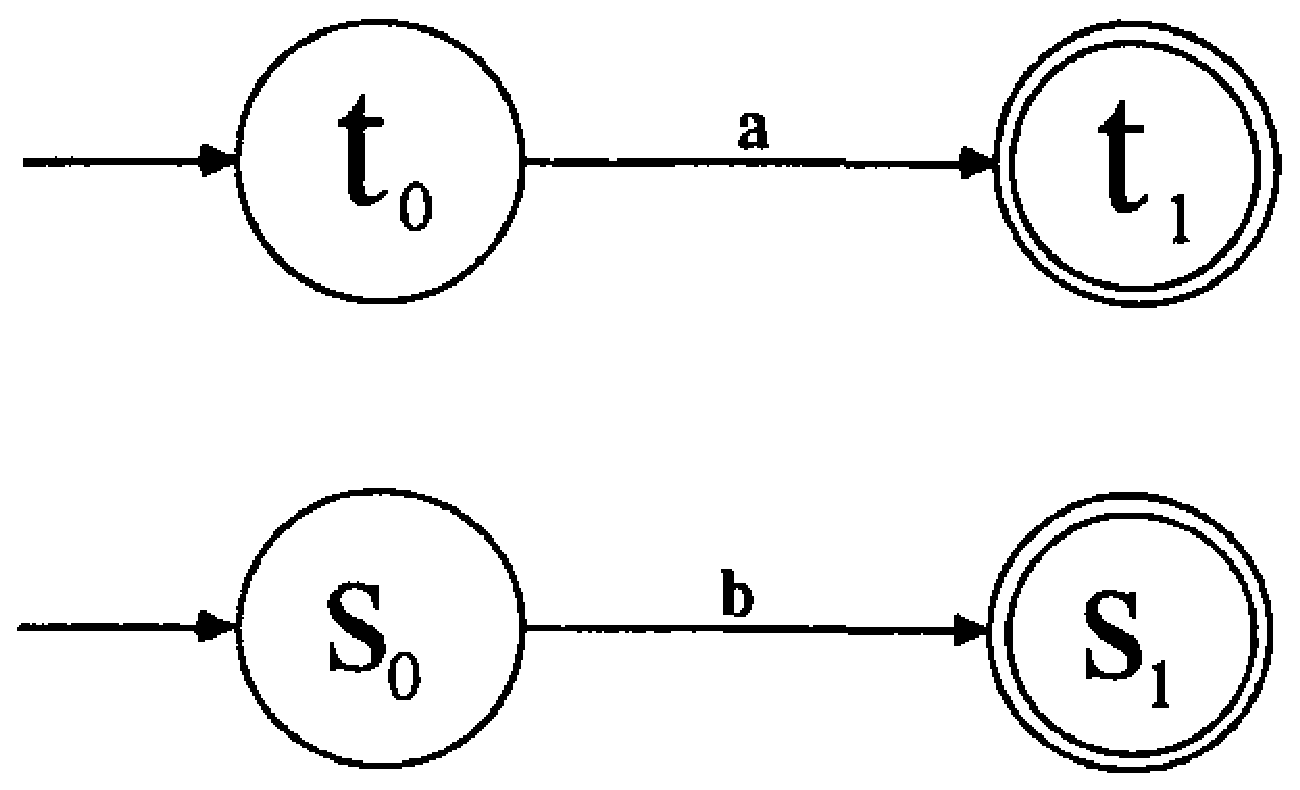
\epsfig{figure=ToFAfigures/fig6-2.eps,width=2.5in}}
\caption{The NDFA discussed in Example 6.4}\label{fig-6.2}
\end{figure}

\subsection*{Example 6.5}

An NDFA that accepts $(\pmb{a}\cup\pmb{b})^*$ is shown in Figure \ref{fig-6.3}. The
automaton given in Figure \ref{fig-6.2} for $(\pmb{a}\cup\pmb{b})$ is modified as
suggested by the proof of Theorem \ref{thm-5.5} to produce the \Index{Kleene closure} of
$(\pmb{a}\cup\pmb{b})$. Recall that the ``extra'' state $q_0$ was added to
ensure that $\lambda$ is accepted by the new machine.

% Figure 6.3
\begin{figure}
\centerline{\epsfig{figure=ToFAfigures/fig6-3.eps,width=2.5in}}
\caption{The NDFA discussed in Example 6.5}\label{fig-6.3}
\end{figure}

\subsection*{Example 6.6}

An NDFA that accepts $\pmb{c}\cdot(\pmb{a}\cup\pmb{b})^*$ (as suggested by the
proof of Theorem \ref{thm-5.4}) is shown in Figure \ref{fig-6.4}.

% Figure 6.4
\begin{figure}
\centerline{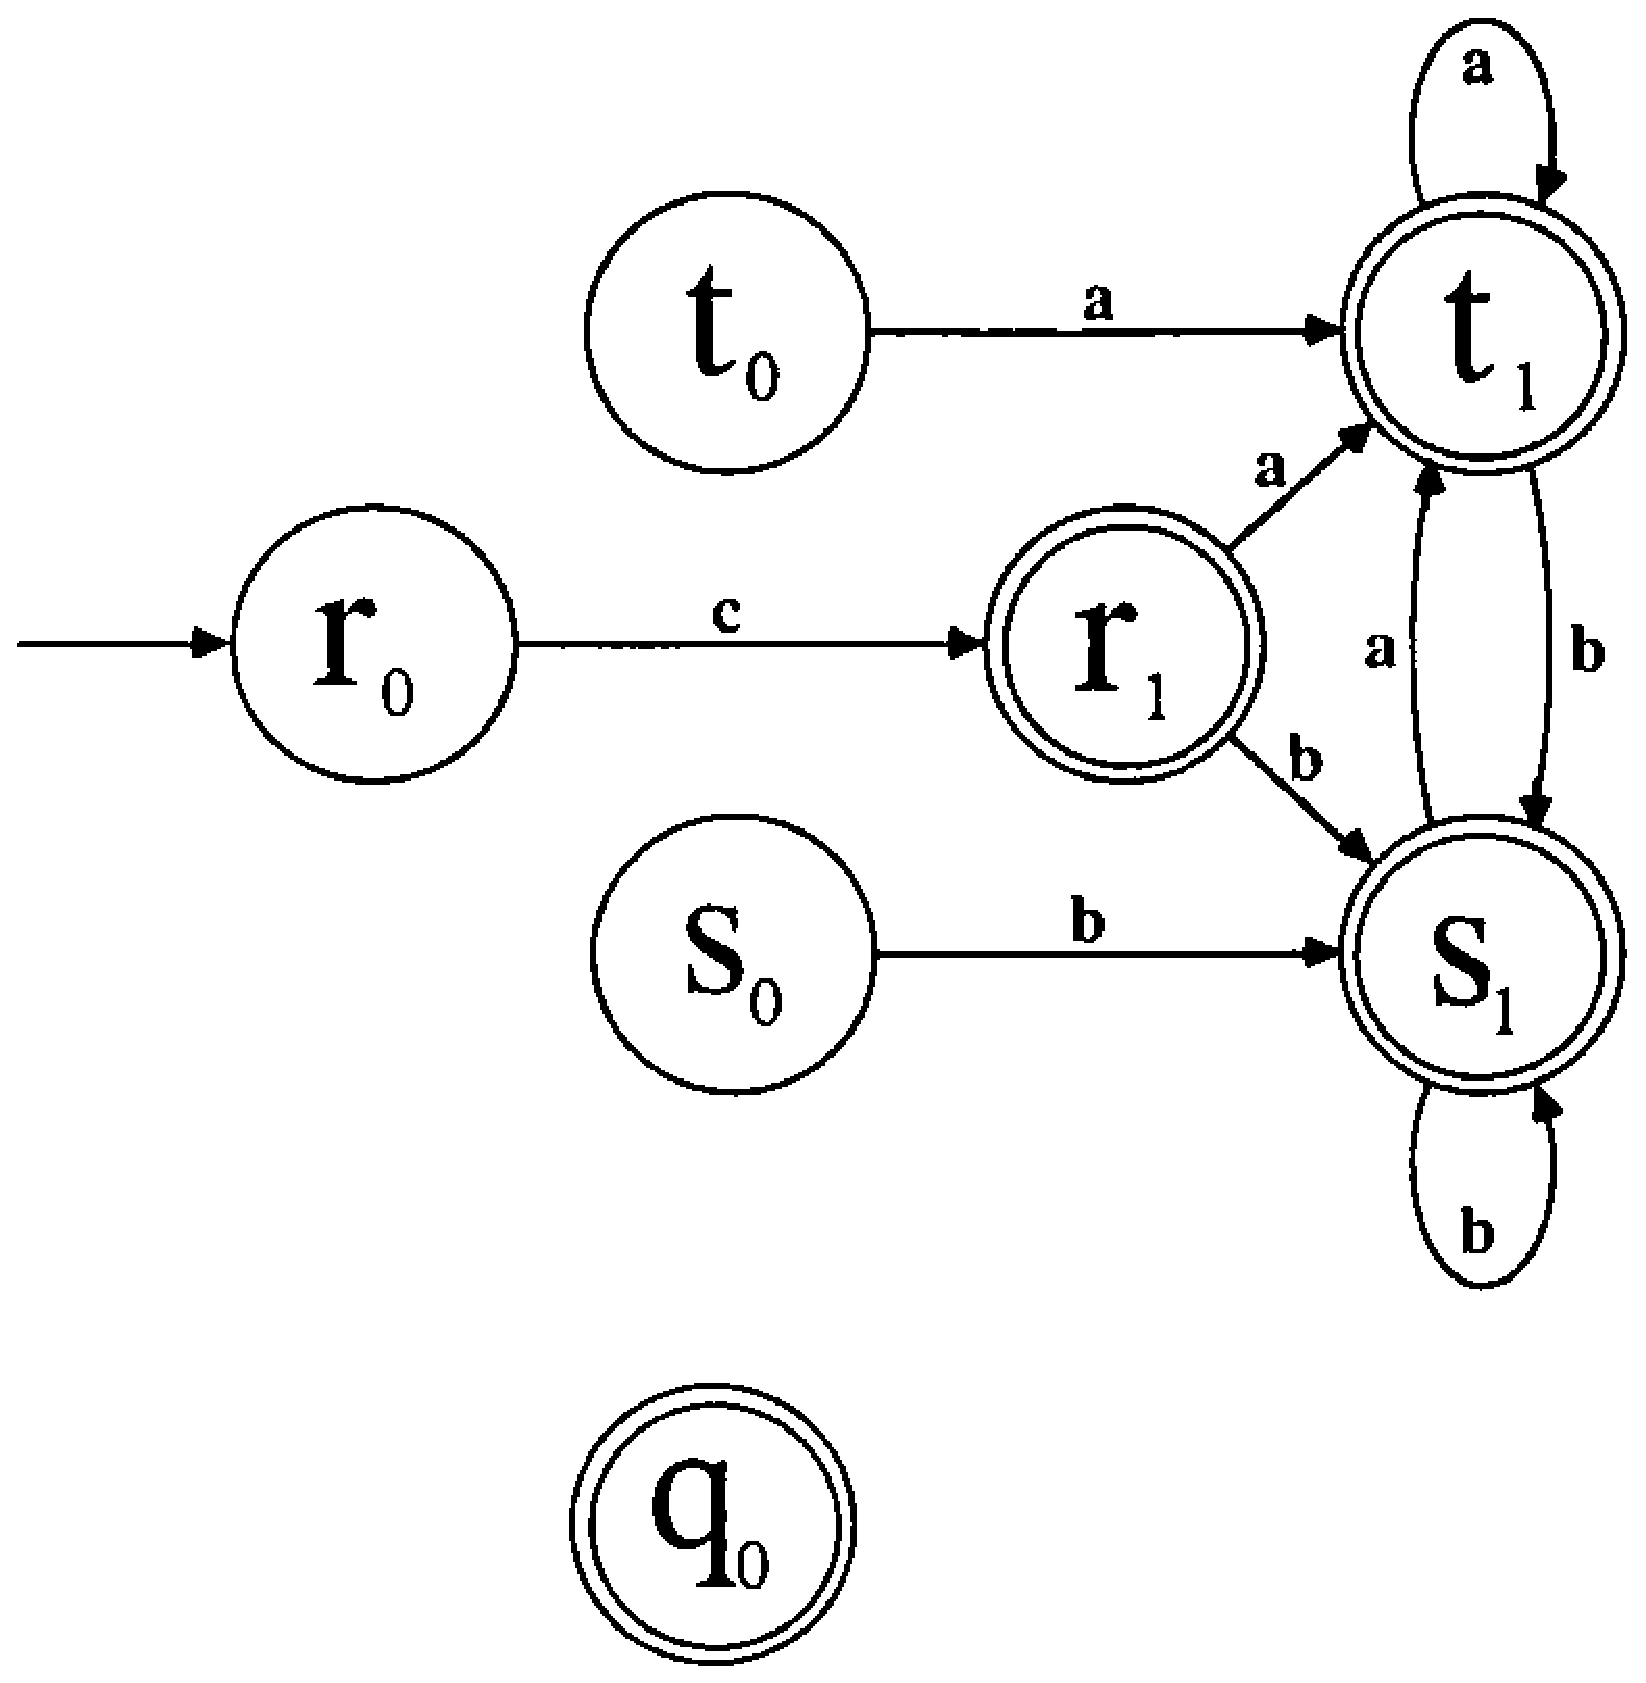
\epsfig{figure=ToFAfigures/fig6-4.eps,width=3.5in}}
\caption{The NDFA discussed in Example 6.6}\label{fig-6.4}
\end{figure}

Note that in this last example $q_0$, $t_0$, and $s_0$ are disconnected states,
and $r_1$, $s_1$, and $t_1$ could be coalesced into a single state. The
resulting machines are not advertised to be \emph{efficient}; the main point is that
they can be built. The techniques illustrated above are used to prove the
following lemma.

% Lemma 6.2
\begin{lmm}\label{lmm-6.2}
Let $\Sigma$ be an alphabet and let $R$ be a regular set over $\Sigma$. Then
there is a DFA that accepts $R$.

\emph{Proof.} The proof is by induction on the number of operators in the
regular expression describing $R$ (see the exercises). Note that Figure \ref{fig-6.1}
effectively illustrates the basis step: Those regular expressions with
\emph{zero} operators ($\emptyset,\epsilon,\pmb{a}_1,\pmb{a}_2,\ldots,\pmb{a}_m$)
do indeed correspond to FAD languages. This covers sets generated by rules i,
ii, and iii of Definition \ref{dfn-6.2}. For sets corresponding to regular expressions
with a positive number of operators, the outermost operator can be identified,
and it will be either $\cdot$, $\cup$, or $^*$, corresponding to an application
of rule iv, v, or vi. The induction assumption will guarantee that the
subexpressions used by the outermost operator have corresponding DFAs. Theorems
\ref{thm-5.2}, \ref{thm-5.4}, and \ref{thm-5.5} can then be invoked to argue that the entire expression has a
corresponding DFA.
\end{lmm}

% Corollary 6.1
\begin{cor}\label{cor-6.1}
Let $\Sigma$ be an alphabet. Then $\RSIG \subseteq \DSIG$.

\emph{Proof.} The proof follows immediately from Lemma \ref{lmm-6.2}.
\end{cor}

Since we are assured that every regular set can be accepted by a finite
automaton, the collection of regular sets is clearly contained in the set of FAD
languages. This also means that those languages that cannot be represented by a
DFA (that is, those contained in \NSIG) have no chance of being represented by a
regular expression.

\section{Language Equations}\label{sec-6.3}

The next question we will address is whether $\DSIG \subseteq \RSIG$, that is,
whether every FAD language can be represented by a regular expression. The
reader is invited to take a sample DFA and try to express the language it
accepts by a regular expression. You will probably be able to do it, but only by
guesswork and trial and error. Our first question appears to have a much more
methodical solution: Given a regular expression, it was a relatively
straightforward task to draw a NDFA (and then a DFA); in fact, we have a set of
\emph{algorithms} for doing just that, and we could program a computer to do the
task for us. This second question does not seem to have an obvious algorithm
connected with it, and we will have to attack the problem using a new concept:
\emph{\Index{language equations}}.

In algebra, we are used to algebraic equations such as $3x + 7 = 19$. Recall
that a \emph{solution} to this equation is a numerical value for $x$ that will make the
equation \emph{true}, that is, make both sides equal. In the above example, there is
only one choice for $x$, the unique solution 4. Equations can have two different
solutions, like $x^2=9$, no [real] solutions, like $x^2=-9$, or an \emph{infinite}
number of solutions, like $2(x+3) = x + 6 + x$. In a similar way, set equations
can be solved, such as $\{\pmb{a},\pmb{b},\pmb{c}\}=\{\pmb{a},\pmb{b}\}\cup X$.
Here $X$ represents a \emph{set}, and we are again looking for a value for $X$ that
will make the equation true; an obvious choice is $X=\{\pmb{c}\}$, but there are
other choices, like $X=\{\pmb{b},\pmb{c}\}$ (since $\{\pmb{a},\pmb{b},\pmb{c}\}=
\{\pmb{a},\pmb{b}\}\cup\{\pmb{b},\pmb{c}\})$. Such equations may likewise have
no solutions, like $X\cup\{\pmb{b}\}=\{\pmb{a},\pmb{c}\}$, or an infinite number
of solutions, such as $X\cup\{\pmb{b}\}=X$ (what sorts of sets satisfy this last
equation?). We wish to look at set equations where the sets are actually sets of
strings, that is, \emph{language} equations. The type of equation in which we
are most interested has one and only one solution, as outlined in the next
theorem. It is very similar in form and spirit to the theorem in algebra that
says ``For any numbers $a$ and $b$, where $a \not= 0$, the equation $ax=b$ has a
unique solution given by $x=b \div a$.''

% Theorem 6.1
\begin{thm}\label{thm-6.1}
Let $\Sigma$ be an alphabet. Let $E$ and $A$ be any subsets of $\Sigma^*$. Then
the language equation $X = E \cup A \cdot X$ admits the solution $X=A^*\!\!\cdot E$.
Any other solution $Y$ must contain $A^*\!\!\cdot E$.
Furthermore, if  $\lambda \notin A$, $X = A^*\!\!\cdot E$ is the unique solution.

\emph{Proof.} First note that the set $A^*E$ is indeed a solution to this
equation, since $A^*E = E \cup A \cdot (A^*E)$ (see the exercises). Now assume
that some set $Y$ is a solution to this equation, and let us investigate some of
the properties that $Y$ must have: If $Y$ is a solution, then
\begin{center}\begin{tabular}{rcl}
$Y = E \cup A \cdot Y$ & $\Rightarrow$ & (by definition of $\cup$) \\
$E \subseteq Y \wedge A \cdot Y \subseteq Y$ & $\Rightarrow$ &
	(if $E \subseteq Y$, then $A \cdot E \subseteq A \cdot Y$) \\
$A \cdot E \subseteq A \cdot Y \subseteq Y$ & $\Rightarrow$ & (by substitution) \\
$A \cdot A \cdot E \subseteq A \cdot A \cdot Y \subseteq A \cdot Y \subseteq Y$
	& $\Rightarrow$ & (by induction) \\
$(\forall n \in \NN)(A^n \cdot E \subseteq Y)$ & $\Rightarrow$ & (by definition
	of $A^*$) \\
$A^*\!\!\cdot E \subseteq Y$ &&
\end{tabular}\end{center}

Thus, every solution must contain all of $A^*E$, and $A^*E$ is in this sense the
smallest solution. This is true regardless of whether or not $\lambda$ belongs
to $A$.

Now let us assume that $\lambda \notin A$ and that we have a solution $W$ that
is actually ``bigger'' than $A^*E$; we will show that this is a contradiction,
and thus all solutions must look \emph{exactly} like $A^*E$. If $W$ is a
solution, $W \not= A^*E$, then there must be some elements in the set $W-A^*E$;
choose a string of \emph{minimal length} from among these elements and call it
$z$. Thus $z \in W$ and $z \notin A^*E$, and since $E \subseteq A^*E$ (why?),
$z \notin E$. Since $W$ is a solution, we have
\begin{center}\begin{tabular}{rcl}
$W=E \cup A \cdot W$ & $\Rightarrow$ & (since $z \in W$ and it cannot be in the
	$E$ part) \\
$z \in A \cdot W$ & $\Rightarrow$ & (by definition of $\cdot$) \\
$(\exists x \in A,\exists y \in W) \ni z = x \cdot y$ & $\Rightarrow$ & (by
	definition of $|\ |$) \\
$|z| = |x| + |y|$ & $\Rightarrow$ & (since $\lambda \notin A$ and $x \in A$, so
	$x \neq \lambda$ and $|x| > 0$) \\
|y| < |z|
\end{tabular}\end{center}

Note that $y$ cannot belong to $A^*E$ (if $y \in A^*E$, then, since $x \in A$,
$z(=x\cdot y)\in A \cdot (A^*E) \subseteq A^*E$, which means that $z \in A^*E$,
and we started by assuming that $z \notin A^*E$); since $y \in W$, we have 
$y \in W - A^*E$, and we have produced a string shorter than $z$, which belongs
to $W - A^*E$. This is the contradiction we were looking for, and we can
conclude that it is impossible for a solution $W$ to be larger than $A^*E$.
Since we have already shown that no solution can be smaller than $A^*E$, we now
know that the only solution is \emph{exactly} $A^*E$.
\end{thm}

\subsection*{Example 6.7}

$X=\{\pmb{b},\pmb{c}\} \cup \{\pmb{a}\} \cdot X$ does indeed have a solution;
$X$ can equal $\{\pmb{a}\}^*\!\!\cdot \{\pmb{b},\pmb{c}\}$. Note also that this is
the only solution (verify, for example, that $X=\{\pmb{a}\}^*\!\!\cdot\{\pmb{c}\}$
is \emph{not} a solution). The equation $Z=\{\pmb{b},\pmb{c}\}\cup\{\pmb{a},\lambda\}
\cdot Z$ has several solutions; among them are $Z=\{\pmb{a}\}^*\!\!\cdot\{\pmb{b},
\pmb{c}\}$ and $Z=\{\pmb{a},\pmb{b},\pmb{c}\}^*$.

It is instructive to explicitly list the first few elements of $\{\pmb{a}\}^*
\!\!\cdot\{\pmb{b},\pmb{c}\}$ and begin to check the validity of the solution to the
first equation. If $Y$ is a solution, then the two sides of the equation
$Y=\{\pmb{b},\pmb{c}\}\cup\{\pmb{a}\}\cdot Y$ must be equal. Since both $\pmb{b}$
and $\pmb{c}$ appear on the right-hand side they must also be on the left-hand
side, which clearly means that they have to be in $Y$. Once $\pmb{b}$ is known to
be in $Y$, it will give rise to a term on the right-hand side due to the
presence of $\{\pmb{a}\}\cdot Y$. Thus, $\pmb{a}\cdot\pmb{b}$ must also be found
on the left-hand side and therefore is in $Y$, and so on. The resulting sequence
of implications parallels the first part of the proof of Theorem \ref{thm-6.1}.

To see intuitively why no string other than those found in $\{\pmb{a}\}^*\cdot
\{\pmb{b},\pmb{c}\}$ may belong to a solution for $X=\{\pmb{b},\pmb{c}\}\cup\{
\pmb{a}\}\cdot X$, consider a string such as $\pmb{aa}$. If this were to belong to
$X$, then it would appear on the left-hand side and therefore would have to
appear on the right-hand side as well if the two sides were to indeed be equal.
On the right-hand side are just the two components, $\{\pmb{b},\pmb{c}\}$ and
$\{\pmb{a}\}\cdot X$. $\pmb{aa}$ is clearly not in $\{\pmb{b},\pmb{c}\}$, so it
must be in $\{\pmb{a}\}\cdot X$, which does seem plausible; all that is
necessary is for $\pmb{a}$ to be in $X$, and then \pmb{aa} will belong to $\{\pmb{a}\}
\cdot X$. If $\pmb{a}$ is in $X$, though, it must also appear on the left-hand
side, and so $\pmb{a}$ must be on the right-hand side as well. Again, $\pmb{a}$ is
not in $\{\pmb{b},\pmb{c}\}$, so it must be in $\{\pmb{a}\}\cdot X$. This can
happen only if $\lambda$ belongs to $X$ so that $\pmb{a}\cdot\lambda$ will
belong to $\{\pmb{a}\}\cdot X$. This implies that $\lambda$ must now show up on
both sides, and this leads to a contradiction: $\lambda$ cannot be on the
right-hand side since $\lambda$ clearly is not in $\{\pmb{b},\pmb{c}\}$, and it
cannot belong to $\{\pmb{a}\}\cdot X$ either, since all these words begin with
an $\pmb{a}$. This contradiction shows why $\pmb{aa}$ cannot be part of any solution
$X$.

This example illustrates the basic nature of these types of equations: for words
that are not in $\{\pmb{a}\}^*\!\!\cdot\{\pmb{b},\pmb{c}\}$, the inclusion of that
word in the solution leads to the inclusion of shorter and shorter strings,
which eventually leads to a contradiction. This property was exploited in the
second half of the proof of Theorem \ref{thm-6.1}. Rather than finding shorter and shorter
strings, though, it was assumed we already had the shortest, and we showed that
there had to be a still shorter one; this led to the desired contradiction more
directly.

Our main goal will be to solve \emph{systems} of language equations, since the
relationships between the \emph{terminal sets} of an automaton can be described
by such a system. Systems of language equations are similar in form and spirit
to systems of algebraic equations, such as
\begin{center}\begin{tabular}{c}
$3x_1 + x_2 = 10$ \\
$x_1 - x_2 = 2$
\end{tabular}\end{center}
which has the unique solution $x_1 = 3$, $x_2 = 1$. We will look at systems of
language equations such as
\begin{center}\begin{tabular}{l}
$X_1 = \epsilon \cup \pmb{a} \cdot X_1 \cup \pmb{b} \cdot X_2$ \\
$X_2 = \emptyset \cup \pmb{b} \cdot X_1 \cup \emptyset \cdot X_2$
\end{tabular}\end{center}
which has the (unique) solution $X_1=(\pmb{a}\cup\pmb{bb})^*,X_2=\pmb{b}\cdot(
\pmb{a}\cup\pmb{bb})^*$. Checking that this is a solution entails verifying that
both equations are satisfied if these expressions are substituted for the
variables $X_1$ and $X_2$.

The solution of such systems parallels the solution of algebraic equations.
For example, the system
\begin{center}\begin{tabular}{c}
$3x_1 + x_2 = 10$ \\
$x_1 - x_2 = 2$
\end{tabular}\end{center}
can be solved by treating the second statement as an equation in just the
variable $x_2$ and solving as indicated by the algebraic theorem ``For any
numbers $a$ and $b$, where $a \not= 0$, the equation $ax = b$ has a unique
solution given by $x = b \div a$.'' The second statement can be written as
$(-1)x_2 = 2 - x_1$, which then admits the solution $x_2=(2-x_1)\div(-1)$ or
$x_2=x_1-2$. This solution can be inserted into the first equation to eliminate
$x_2$ and form an equation solely in $x_1$. Terms can be regrouped and the
algebraic theorem can be applied to find $x_1$. We would have
\[ 3x_1 + x_2 = 10 \]
which becomes
\[ 3x_1 + x_1 - 2 = 10 \]
or
\[ 4x_1 - 2 = 10 \]
or
\[ 4x_1 = 12 \]
or
\[ x_1 = 12 \div 4 \]
yielding
\[ x_1 = 3 \]
This value of $x_1$ can be back-substituted to find the unique solution for
$x_2$: $x_2=x_1-2=3-2=1$.

Essentially, the same technique can be applied to any two equations in two
unknowns, and formulas can be developed that predict the coefficients for the
reduced set of equations. Consider the generalized system of algebraic equations
with unknowns $x_1$ and $x_2$, constant terms $E_1$ and $E_2$, and coefficients
$A_{11},\ A_{12},\ A_{21},$ and $A_{22}$:
\begin{center}\begin{tabular}{c}
$A_{11}x_1 + A_{12}x_2 = E_1$ \\
$A_{21}x_1 + A_{22}x_2 = E_2$
\end{tabular}\end{center}
Recall that the appropriate formulas for reducing this to a single equation of
the form $\hat{A}_{11}x_1 = \hat{E}_1$, where the new coefficients
$\hat{A}_{11}$ and $\hat{E}_1$ can be calculated as
\begin{center}\begin{tabular}{c}
$\hat{E}_1 = E_1A_{22} - E_2A_{12}$ \\
$\hat{A}_{11} = A_{11}A_{22} - A_{12}A_{21}$
\end{tabular}\end{center}
A similar technique can be used to eliminate variables when there is a larger
number of equations in the system. The following theorem makes similar
predictions of the new coefficients for language equations.

% Theorem 6.2
\begin{thm}\label{thm-6.2}
Let $n \geq 2$ and consider the system of equations in the unknowns $X_1,X_2,
\ldots,X_n$ given by
\begin{center}\begin{tabular}{rcl}
$X_1$ & $=$ & $E_1 \cup A_{11}X_1 \cup A_{12}X_2 \cup \cdots \cup A_{1(n-1)}
	X_{n-1} \cup A_{1n}X_n$ \\
$X_2$ & $=$ & $E_2 \cup A_{21}X_1 \cup A_{22}X_2 \cup \cdots \cup A_{2(n-1)}
	X_{n-1} \cup A_{2n}X_n$ \\
$\cdot$ && \\
$\cdot$ && \\
$\cdot$ && \\
$X_{n-1}$ & $=$ & $E_{n-1} \cup A_{(n-1)1}X_1 \cup A_{(n-1)2}X_2 \cup \cdots
	\cup A_{(n-1)(n-1)}X_{n-1} \cup A_{(n-1)n}X_n$ \\
$X_n$ & $=$ & $E_n \cup A_{n1}X_1 \cup A_{n2}X_2 \cup \cdots \cup
	A_{n(n-1)}X_{n-1} \cup A_{nn}X_n$
\end{tabular}\end{center}
in which $(\forall i,j \in \{1,2, \cdots ,n\})(\lambda \notin A_{ij})$.
\begin{enumerate}[a.]
\item This system has a unique solution.
\item Define $\hat{E}_i = E_i \cup (A_{in} \cdot A^*_{nn} \cdot E_n)$ for all
	$i=1,2, \cdots ,n - 1$ \\
and
\[ \hat{A}_{ij} = A_{ij} \cup (A_{in} \cdot A^*_{nn} \cdot A_{nj})\text{ for
	all }i,j = 1,2, \cdots ,n - 1. \]
The solution to the original set of equations will agree with the solution to
the following set of $n-1$ equations in the unknowns $X_1,X_2,\cdots,X_{n-1}$:
\begin{center}\begin{tabular}{rcl}
$X_1$ & $=$ & $\hat{E}_1 \cup \hat{A}_{11}X_1 \cup \hat{A}_{12}X_2 \cup \cdots
	\cup \hat{A}_{1(n-1)}X_{n-1}$ \\
$X_2$ & $=$ & $\hat{E}_2 \cup \hat{A}_{21}X_1 \cup \hat{A}_{22}X_2 \cup \cdots
	\cup \hat{A}_{2(n-2)}X_{n-1}$ \\
$\cdot$ && \\
$\cdot$ && \\
$\cdot$ && \\
$X_{n-1}$ & $=$ & $\hat{E}_{n-1} \cup \hat{A}_{(n-1)1}X_1 \cup \hat{A}_{(n-1)2}
	X_2 \cup \cdots \cup \hat{A}_{(n-1)(n-1)}X_{n-1}$
\end{tabular}\end{center}
\item Once the solution to the above $n - 1$ equations in (b) is known, that
solution can be used to find the remaining unknown:
\[ X_n = A^*_{nn} \cdot (E_n \cup A_{n1}X_1 \cup A_{n2}X_2 \cup \cdots \cup
	A_{n(n-1)}X_{n-1}) \]
\end{enumerate}

\emph{Proof.} The proof hinges on the repeated application of Theorem \ref{thm-6.1}. The
last of the $n$ equations, $X_n = E_n \cup A_{n1}X_1 \cup A_{n2}X_2 \cup \cdots
\cup A_{n(n-1)}X_{n-1} \cup A_{nn}X_{n}$ can be thought of as an equation in the
one unknown $X_n$ with a coefficient of $A_{nn}$ for $X_n$, and the remainder of
the expression a ``constant'' term not involving $X_n$. The following
parenthetical grouping illustrates this viewpoint:
\[ X_n = (E_n \cup A_{n1}X_1 \cup A_{n2}X_2 \cup \cdots \cup A_{n(n-1)}X_{n-1})
	\cup A_{nn}X_n \]
Note that for any subscript $k$, if $A_{nk}$ does not contain $\lambda$, neither
will $A_{nk}X_k$. Theorem \ref{thm-6.1} can therefore be applied, to the one equation in
the one unknown $X_n$, with coefficients
\[ E = (E_n \cup A_{n1}X_1 \cup A_{n2}X_2 \cup \cdots \cup A_{n(n-1)}X_{n-1}) \]
and $A = A_{nn}$. The solution, $A^*E$, is exactly as given by part (c) above:
\[ X_n = A^*_{nn} \cdot (E_n \cup A_{n1}X_1 \cup A_{n2}X_2 \cup \cdots \cup
	A_{n(n-1)}X_{n-1}) \]
or
\[ X_n = A^*_{nn} \cdot E_n \cup A^*_{nn} \cdot A_{n1}X_1 \cup A^*_{nn} \cdot
	A_{n2}X_2 \cup \cdots \cup A^*_{nn} \cdot A_{n(n-1)}X_{n-1} \]
If there was a unique solution for the terms $X_1$ through $X_{n-1}$, then
Theorem \ref{thm-6.1} would guarantee a unique solution for $X_n$, too.

The solution for $X_n$ can be substituted for $X_n$ in each of the other $n-1$
equations. If the $k$th equation is represented by
\[ X_k = E_k \cup A_{k1}X_1 \cup A_{k2}X_2 \cup \cdots \cup A_{kn}X_n \]
then the substitution will yield \\
\begin{tabular}{lll}
$X_k$ & $=$ & $E_k \cup A_{k1}X_1 \cup A_{k2}X_2 \cup \cdots$ \\
&& $\cup (A_{kn} \cdot (A^*_{nn} \cdot E_n \cup A^*_{nn} \cdot A_{n1}X_1 \cup
	A^*_{nn} \cdot A_{n2}X_2 \cup \cdots \cup A^*_{nn} \cdot
	A_{n(n-1)}X_{n-1}))$
\end{tabular} \\
By using the distributive law, this becomes \\
\begin{tabular}{lll}
$X_k$ & $=$ & $E_k \cup A_{k1}X_1 \cup A_{k2}X_2 \cup \cdots$ \\
&& $\cup (A_{kn} \cdot A^*_{nn} \cdot E_n \cup A_{kn} \cdot A^*_{nn} \cdot
	A_{n1}X_1 \cup A_{kn} \cdot A^*_{nn} \cdot A_{n2}X_2 \cup \cdots \cup
	A_{kn} \cdot A^*_{nn} \cdot A_{n(n-1)}X_{n-1})$
\end{tabular} \\
Collecting like terms yields \\
\begin{tabular}{lll}
$X_k$ & $=$ & $(E_k \cup A_{kn} \cdot A^*_{nn} \cdot E_n) \cup (A_{k1}X_1 \cup
	A_{kn} \cdot A^*_{nn} \cdot A_{n1}X_1)$ \\
&& $\cup (A_{k2}X_2 \cup A_{kn} \cdot A^*_{nn} \cdot A_{n2}X_2) \cup \cdots \cup
	(A_{k(n-1)}X_{n-1} \cup A_{kn} \cdot A^*_{nn} \cdot A_{n(n-1)}X_{n-1})$
\end{tabular} \\
or
\begin{center}\begin{tabular}{l}
$X_k = (E_k \cup A_{kn} \cdot A^*_{nn} \cdot E_n) \cup (A_{k1} \cup A_{kn}
	\cdot A^*_{nn} \cdot A_{n1})X_1$ \\
$\qquad \cup (A_{k2} \cup A_{kn} \cdot A^*_{nn} \cdot A_{n2})X_2 \cup \cdots
	\cup (A_{k(n-1)} \cup A_{kn} \cdot A^*_{nn} \cdot A_{n(n-1)})X_{n-1}$
\end{tabular}\end{center}
The constant term in this equation is $(E_k \cup A_{kn} \cdot A^*_{nn} \cdot
E_n)$, which is exactly the formula given for $\hat{E}_k$ in part (b). The
coefficient for $X_1$ is seen to be
\[ (A_{k1} \cup A_{kn} \cdot A^*_{nn} \cdot A_{n1}), \]
while the coefficient for $X_2$ is $(A_{k2} \cup A_{kn} \cdot A^*_{nn} \cdot
A_{n2})$, and so on. The coefficient for $X_j$ would then be $\hat{A}_{kj} =
A_{kj} \cup (A_{kn} \cdot A^*_{nn} \cdot A_{nj})$, which also agrees with the
formula given in part (b). This is why the solution of the original set of
equations agrees with the solution of the set of $n-1$ equations given in part
(b).

Part (a) is proved by induction on $n$: the method outlined above can be
repeated on the new set of $n-1$ equations to eliminate $X_{n-1}$ and so on,
until one equation in the one unknown $X_1$ is obtained. Theorem \ref{thm-6.1} will
guarantee a unique solution for $X_1$, and part (c) can then be used to find the
unique solution for $X_2$, and so on.
\end{thm}

\subsection*{Example 6.8}

Consider the system defined before, where
\begin{center}\begin{tabular}{r@{ = }l}
$X_1$ & $\epsilon \cup \pmb{a} \cdot X_1 \cup \pmb{b} \cdot X_2$ \\
$X_2$ & $\emptyset \cup \pmb{b} \cdot X_1 \cup \emptyset \cdot X_2$
\end{tabular}\end{center}
The proof of Theorem \ref{thm-6.2} implies the solution for $X_1$ will agree with the
solution to the one-variable equation $X_1 = \hat{E}_1 \cup \hat{A}_{11}X_1$,
where
\[ \hat{E}_1 = E_1 \cup (A_{12}\cdot A^*_{22}\cdot E_2) = \epsilon \cup (\pmb{b} \cdot \emptyset^*\!\!
	\cdot \emptyset) = \epsilon \cup (\pmb{b}\cdot\epsilon\cdot\emptyset) =
	\epsilon \cup \emptyset = \epsilon \]
and
\[ \hat{A}_{11} = A_{11} \cup (A_{12} \cdot A^*_{22} \cdot A_{21}) = \pmb{a}
	\cup (\pmb{b}\cdot\emptyset^*\!\!\cdot\pmb{b}) = \pmb{a} \cup (\pmb{b} \cdot
	\epsilon \cdot \pmb{b}) = \pmb{a} \cup \pmb{bb}. \]
Thus we have $X_1 = \epsilon \cup (\pmb{a} \cup \pmb{bb})\cdot X_1$, which by
Theorem \ref{thm-6.1} has the (unique) solution $X_1 = \hat{A}^*_{11}\hat{E}_1 = (\pmb{a}
\cup \pmb{bb})^*\!\! \cdot \epsilon$. Substituting this into the second equation
yields $X_2 = \emptyset \cup \pmb{b}\cdot(\pmb{a}\cup\pmb{bb})^*\cup\emptyset
\cdot X_2$, which by Theorem \ref{thm-6.1} has the (unique) solution $X_2=\emptyset^*\!\!\cdot
(\pmb{b}\cdot(\pmb{a}\cup\pmb{bb})^*) = \pmb{b} \cdot (\pmb{a}\cup\pmb{bb})^*$\!.
Note that this expression for $X_2$ could also be found by applying the
back-substitution formula given in the proof of Theorem \ref{thm-6.2}.

We will now see that the language accepted by a DFA can be equated with the
solution of a set of language equations, which will allow us to prove the
following important theorem.

% Theorem 6.3
\begin{thm}\label{thm-6.3}
Let $\Sigma$ be an alphabet and let $L$ be an FAD language over $\Sigma$. Then
$L$ is a regular set over $\Sigma$.

\emph{Proof.} If $L$ is FAD, then there exists an $n > 0$ and a deterministic
finite automaton $A=\langle\Sigma,\{s_1,s_2, \ldots,\\s_n\},s_1,\delta,F\rangle$
such that $L(A) = L$. For each $i = 1,2,\ldots ,n,$ define $X_i=\{z \in \Sigma^*
|\ \DBAR(s_i,z) \in F\}$; that is, $X_i$ is the set of all strings that, \emph{when
starting at state} $s_i$, reach a final state in $A$. Each $X_i$ then represents
the terminal set $T(A,s_i)$ described in Chapter \ref{ch-3}. Since $s_1$ is the start state
of this machine, it should be clear that $X_1 = L(A) = L$. Define
\begin{align*}
E_i = & \left\{ \begin{tabular}{ll}
			$\emptyset$ & if $s_i \notin F$ \\
			& \\
			$\epsilon$ & if $s_i \in F$
		 \end{tabular}\right. &
		 \text{for }i = 1,2,\ldots,n \\
\intertext{and}
A_{ij} = & \bigcup\limits_{\pmb{a}\,\in\,\Sigma\,\wedge\,\delta(s_i,\pmb{a})\,=\,
	s_j} \pmb{a} & \text{for }i,j=1,2, \ldots ,n
\end{align*}
That is, $A_{ij}$ represents the set of all letters that cause a transition from
state $s_i$ to state $s_j$. Notice that since $\lambda\notin\Sigma$ none of the
sets $A_{ij}$ contain the empty string, and therefore by Theorem \ref{thm-6.2}, there is a
unique solution to the system:
\begin{center}\begin{tabular}{rcl}
$X_1$ & $=$ & $E_1 \cup A_{11}X_1 \cup A_{12}X_2 \cup \cdots \cup A_{1n}X_n$ \\
$X_2$ & $=$ & $E_2 \cup A_{21}X_1 \cup A_{22}X_2 \cup \cdots \cup A_{2n}X_n$ \\
& $\cdot$ & \\ & $\cdot$ & \\ & $\cdot$ & \\
$X_n$ & $=$ & $E_n \cup A_{n1}X_1 \cup A_{n2}X_2 \cup \cdots \cup A_{nn}X_n$
\end{tabular}\end{center}
However, these equations exactly describe the relationships between the terminal
sets denoted by $X_1,X_2, \cdots ,\\X_n$, at the beginning of this proof (compare
with Example 6.11), and hence the solution will represent exactly those
quantities. In particular, the solution for $X_1$ will be a regular expression
for $L(A)$, that is, for $L$.
\end{thm}

\subsection*{Example 6.9}

Consider the DFA $B$ given by the diagram in Figure \ref{fig-6.5}, which accepts all
strings with an odd number of $\pmb{b}$s over $\{\pmb{a},\pmb{b}\}$. This machine
generates the following system of language equations:
\begin{align*}
& X_1 = \emptyset \cup \pmb{a}X_1 \cup \pmb{b}X_2 \\
& X_2 = \epsilon \cup \pmb{b}X_1 \cup \pmb{a}X_2
\end{align*}
which will have the same solution for $X_1$ as the equation
\[ X_1 = \hat{E}_1 \cup \hat{A}_{11}X_1 \]
where
\[ \hat{E}_1 = E_1 \cup (A_{12}\cdot A^*_{22}\cdot E_2) = \emptyset \cup
	(\pmb{b}\cdot\pmb{a}^*\cdot\epsilon) = \pmb{b}\cdot\pmb{a}^* \]
and
\[ \hat{A}_{11} = A_{11} \cup (A_{12}\cdot A^*_{22}\cdot A_{21}) = \pmb{a} \cup
	(\pmb{b}\cdot\pmb{a}^*\cdot\pmb{b}) \]
% Figure 6.5
\begin{figure}
\centerline{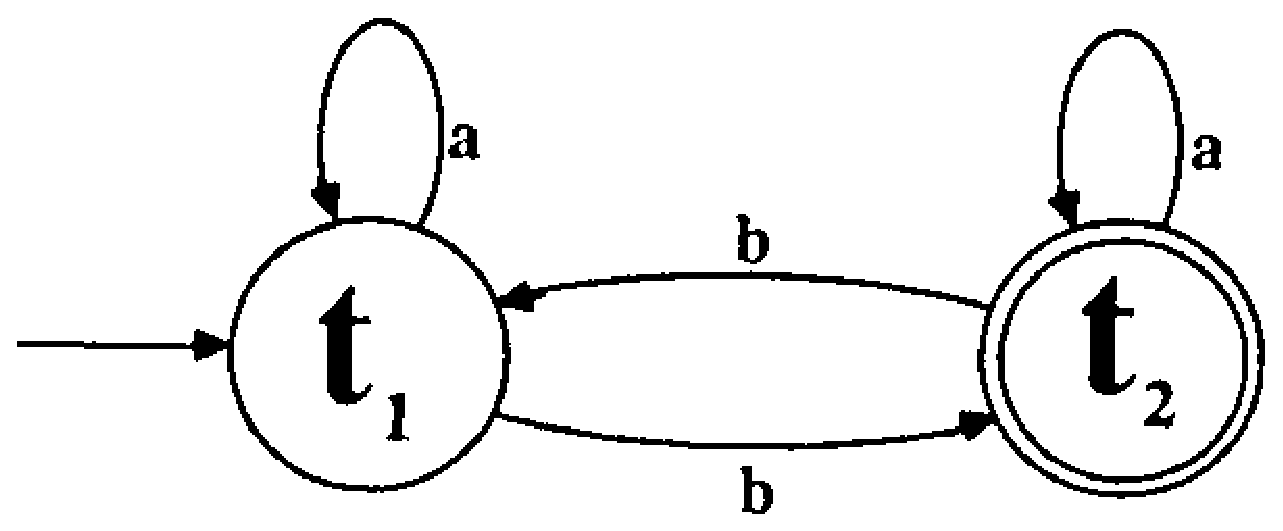
\epsfig{figure=ToFAfigures/fig6-5.eps,width=2.5in}}
\caption{The DFA discussed in Example 6.9}\label{fig-6.5}
\end{figure}
Theorem \ref{thm-6.1} predicts the solution for $X_1$ to be $(\pmb{a}\cup(\pmb{b}\cdot
\pmb{a}^*\cdot\pmb{b}))^*\cdot\pmb{b}\cdot\pmb{a}^*$. It can be verified that
this solution describes all those strings with an odd number of $\pmb{b}$s. $X_1$
is indeed the terminal set for $t_1$, that is, $T(B,t_1)$. Likewise, finding
$X_2$ yields all strings with an even number of $\pmb{b}$s, which is the terminal
set for $t_2$, $T(B,t_2)$.

Nondeterministic finite automata can likewise be represented by language
equations, and without the intermediate step of applying Definition \ref{dfn-4.5} to
acquire a deterministic equivalent. The sets $E_i$ and $A_{ij}$ retain
essentially the same definitions as before: $E_i$ is $\epsilon$ or $\emptyset$,
depending on whether or not $s_i$ is a final state, and $A_{ij}$ again
represents exactly the set of all letters that cause a transition from state
$s_i$ to state $s_j$. This definition requires a minor cosmetic change for
NDFAs, since the state transition function is slightly different:
\[ A_{ij} = \bigcup\limits_{\pmb{a}\,\in\,\Sigma\,\wedge\,s_j\,\in\,\delta(s_i,
	\pmb{a})}\pmb{a}\qquad\text{for }i,j=1,2, \ldots ,n \]

An $n$-state NDFA therefore gives rise to $n$ equations in $n$ unknowns, which
can be solved as outlined by Theorems \ref{thm-6.2} and \ref{thm-6.1}. While Definition \ref{dfn-4.5} need not
be used as a conversion step, an NDFA with $\lambda$-moves will have to be
transformed into an equivalent NDFA without $\lambda$-moves. An appropriate
definition for $A_{ij}$ \emph{could} be given for the original NDFA, and while
the resulting equations would describe the relation between the terminal sets,
some $A_{ij}$ set might then contain $\lambda$ as a member. There are systems of
equations arising in this manner that do not have unique solutions (see the
exercises). For an NDFA with $\lambda$-moves, Definition \ref{dfn-4.9} could be applied to
find an equivalent NDFA without $\lambda$-moves, since Theorems \ref{thm-6.2} and \ref{thm-6.1}
specifically prohibit the empty string as a part of a coefficient. However, if
the ambiguous equations generated from a machine with $\lambda$-moves were
solved as suggested in Theorems \ref{thm-6.1} and \ref{thm-6.2}, a ``minimal'' solution would be
obtained that would correspond to the desired answer.

\subsection*{Example 6.10}

Consider again the system described in Example 6.8. This can be thought of as
the set of language equations corresponding to the NDFA called $B$, illustrated
in Figure \ref{fig-6.6}a. Note that $L(B)$ is indeed the given solution: $L(B) = X_1 =
(\pmb{a}\cup\pmb{bb})^*$. Notice the similarity between $B$ and the machine $C$
shown in Figure \ref{fig-6.6}b, which has $s_2$ as the start state. Note that $L(C)$ is
given by $X_2=\pmb{b}\cdot(\pmb{a}\cup\pmb{bb})^*$, where $X_2$ was the other
part of the solution given in Example 6.8 (verify this). Finally, consider a
similar machine $D$ in Figure \ref{fig-6.6}c with both $s_1$ and $s_2$ as start states.
Can you quickly write a regular expression that describes the language accepted
by $D$?

% Figure 6.6
\begin{figure}
\centerline{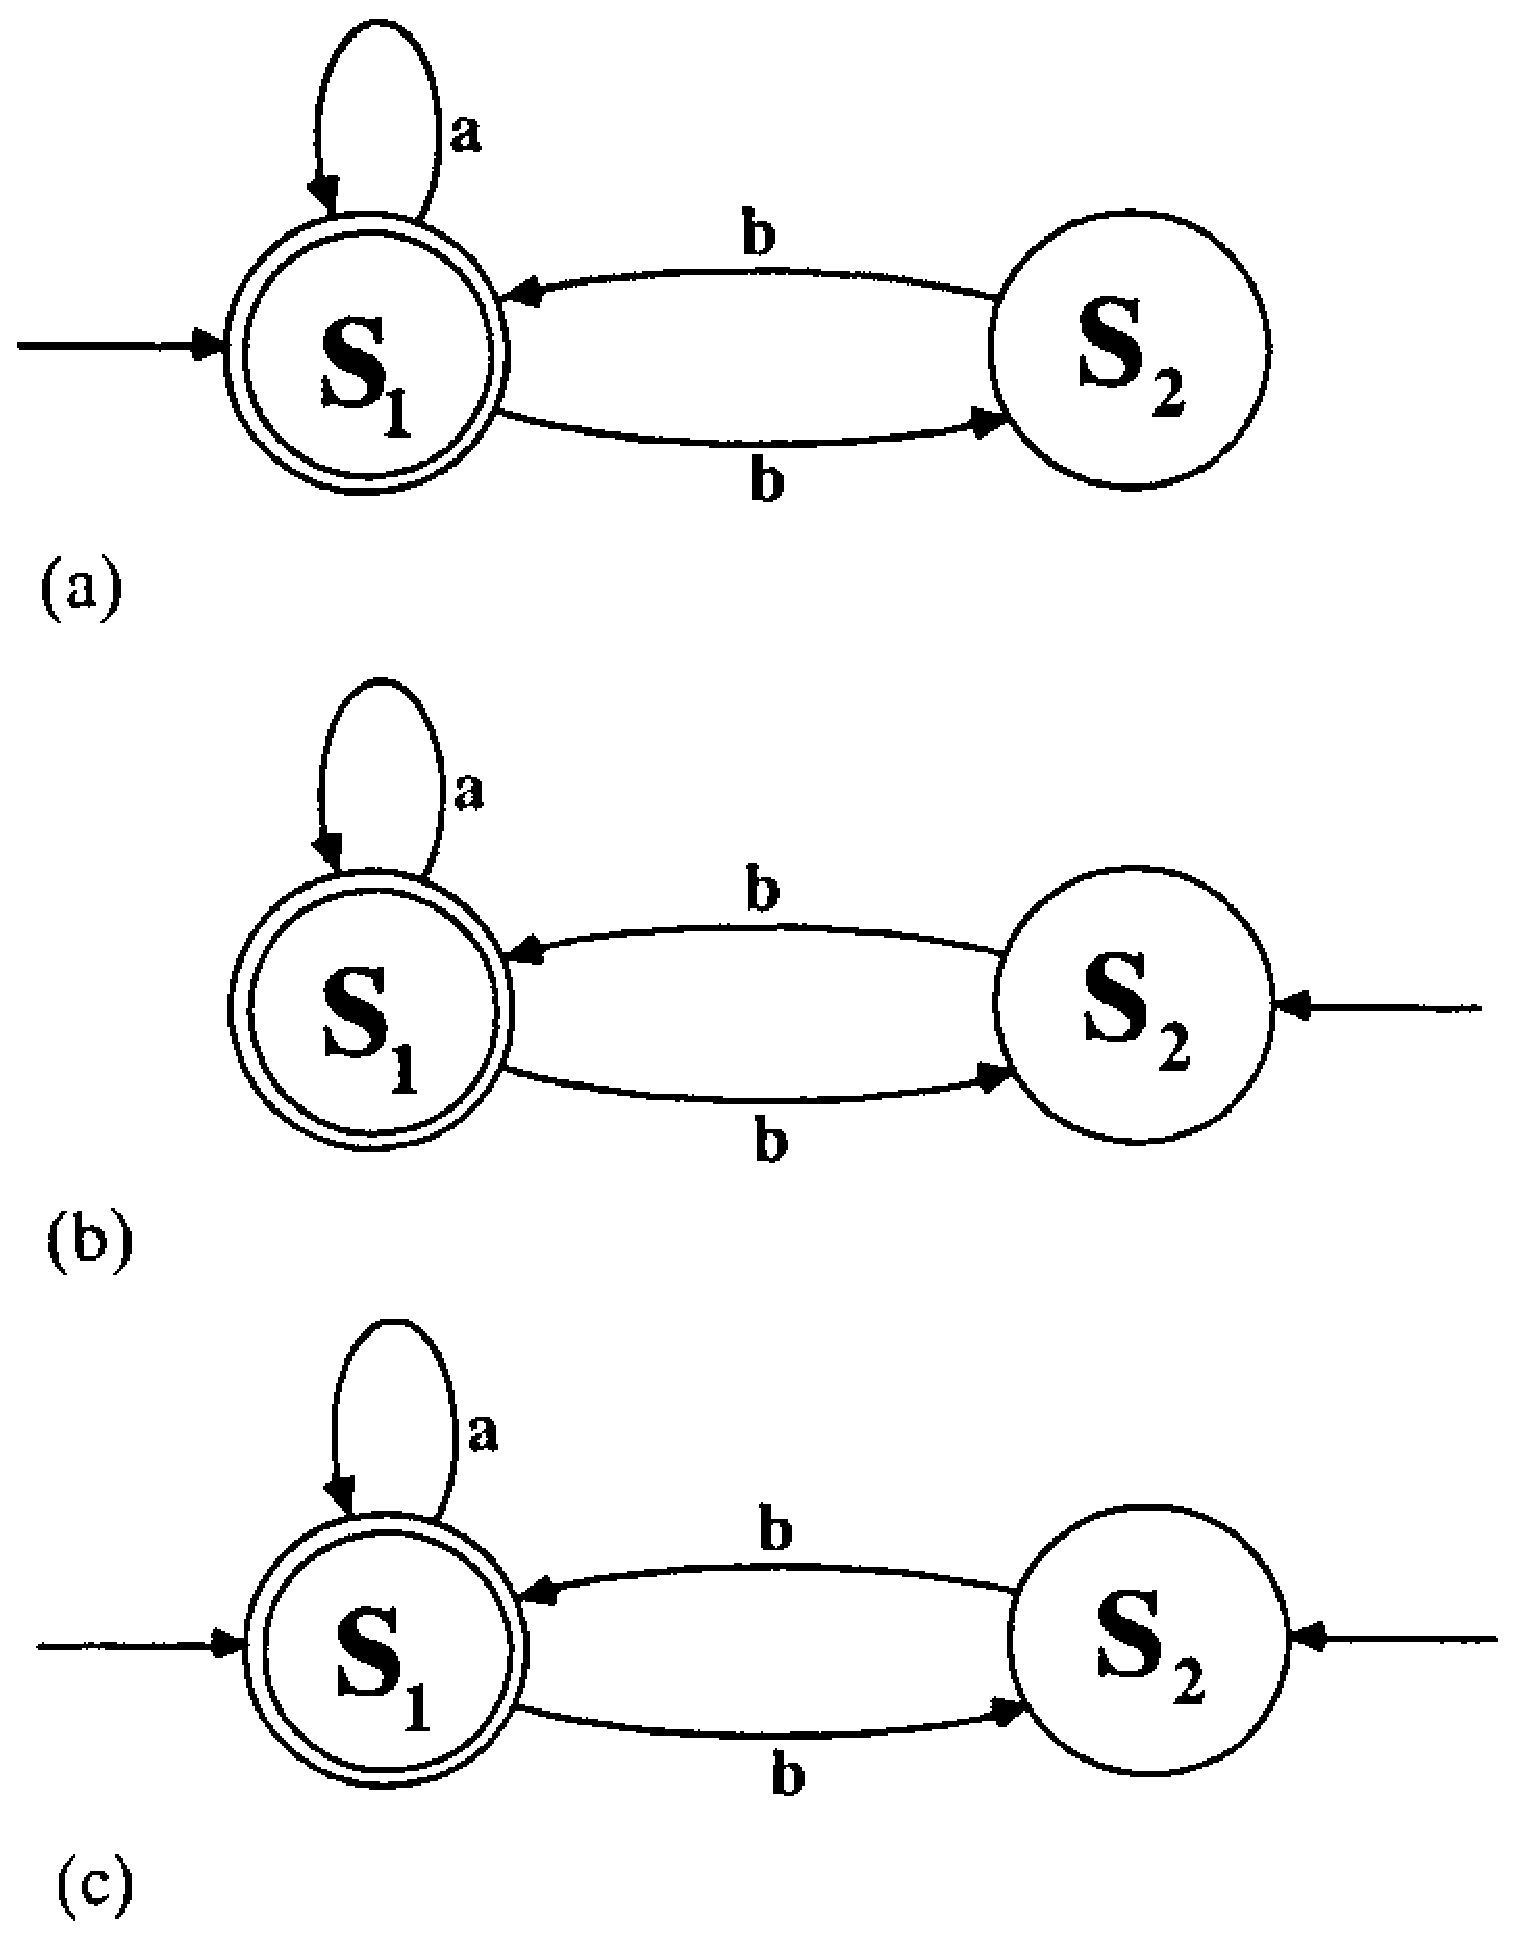
\epsfig{figure=ToFAfigures/fig6-6.eps,width=2.5in}}
\caption{(a) The NDFA $B$ discussed in Example 6.10 (b) The NDFA $C$
discussed in Example 6.10 (c) The NDFA $D$ discussed in Example 6.10}\label{fig-6.6}
\end{figure}

\subsection*{Example 6.11}

% Figure 6.7
\begin{figure}
\centerline{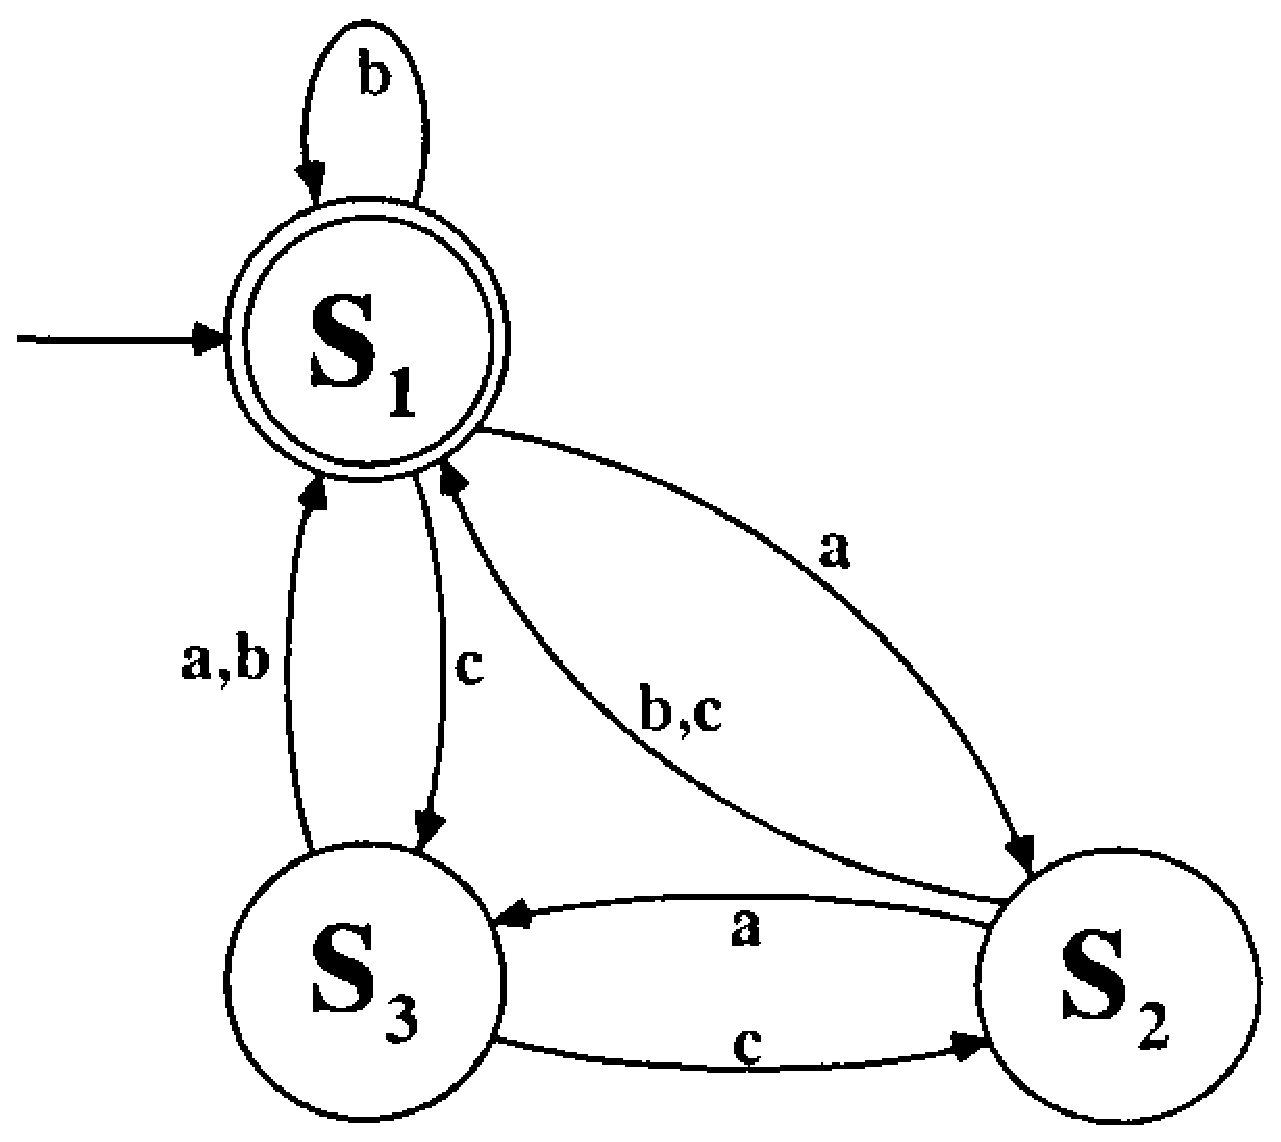
\epsfig{figure=ToFAfigures/fig6-7.eps,width=2.5in}}
\caption{The DFA discussed in Example 6.11}\label{fig-6.7}
\end{figure}

Regular expressions for machines with more than two states can be found by
repeated application of the technique described in Theorem \ref{thm-6.2}. For example,
consider the three-state DFA given in Figure \ref{fig-6.7}. The solution for this
three-state machine will be explored shortly. We begin by illustrating the
natural relationships between the terminal sets described in Theorem \ref{thm-6.3}. First
let us note that the language accepted by this machine includes:
\begin{enumerate}
\item All strings that end with $\pmb{b}$.
\item Strings that contain no $\pmb{b}$s, but for which $|x|_{\pmb{a}} -
	|x|_{\pmb{c}}$ is a multiple of 3.
\item Strings that are concatenations of type (1) and type (2) strings.
\end{enumerate}

According to Theorem \ref{thm-6.3}, the equations for this machine are
\begin{align*}
& X_1 = \epsilon \cup \pmb{b}X_1 \cup \pmb{a}X_2 \cup \pmb{c}X_3 \\
& X_2 = \emptyset \cup (\pmb{b}\cup\pmb{c})X_1 \cup \emptyset X_2 \cup \pmb{a}
	X_3 \\
& X_3 = \emptyset \cup (\pmb{a}\cup\pmb{b})X_1 \cup \pmb{c}X_2 \cup \emptyset
	X_3
\intertext{which can be simplified to}
& X_1 = \epsilon \cup \pmb{b}X_1 \cup \pmb{a}X_2 \cup \pmb{c}X_3 \\
& X_2 = (\pmb{b}\cup\pmb{c})X_1 \cup \pmb{a}X_3 \\
& X_3 = (\pmb{a}\cup\pmb{b})X_1 \cup \pmb{c}X_2
\intertext{and rewritten as}
& X_1 = \epsilon \cup \pmb{b}X_1 \cup \pmb{a}X_2 \cup \pmb{c}X_3 \\
& X_2 = \pmb{b}X_1 \cup \pmb{c}X_1 \cup \pmb{a}X_3 \\
& X_3 = \pmb{a}X_1 \cup \pmb{b}X_1 \cup \pmb{c}X_2
\end{align*}

The equation for $X_1$ admits the following interpretation; recalling that $X_1$
represents all the strings that reach a final state when starting from $s_1$, we
see that these can be broken up into four distinct classes:
\begin{enumerate}
\item Strings of length 0: $(\epsilon)$.
\item Strings that start with $\pmb{a}$ (and note that $\pmb{a}$ moves the current
	state from $s_1$ to $s_2$) and then proceed (from $s_2$) to a final
	state: $(\pmb{a}X_2)$.
\item Strings that start with $\pmb{b}$ and then proceed to a final state:
	$(\pmb{b}X_1)$.
\item Strings that start with $\pmb{c}$ and then proceed to a final state:
	$(\pmb{c}X_3)$.
\end{enumerate}
The union of these four classes should equal $X_1$, which is exactly what the
first equation states.

$X_2 = \pmb{b}X_1 \cup \pmb{c}X_1 \cup \pmb{a}X_3$ can be interpreted similarly;
$\epsilon$ does not appear in this equation because there is \emph{no} way to
reach a final state from $s_2$ if no letters are processed. If at least one
letter is processed, then that first letter is an $\pmb{a}$, $\pmb{b}$, or $\pmb{c}$.
If it is $\pmb{a}$, then we move from state $s_2$ to $s_3$, and the remainder of
the string must take us to a final state from $s_3$ (that is, the remainder must
belong to $X_3$). Strings that begin with an $\pmb{a}$ and are followed by a
string from $X_3$ can easily be described by $\pmb{a}\cdot X_3$. Similarly,
strings that start with $\pmb{b}$ or $\pmb{c}$ must move from $s_2$ to $s_1$, and
then be followed by a string from $X_1$. These strings are described by
$\pmb{b}\cdot X_1$ and $\pmb{c}\cdot X_1$. The three cases for reaching a final
state from $s_2$ that have just been described are exhaustive (and mutually
exclusive), and so their union should equal all of $X_2$. This is exactly the
relation expressed by the second equation, $X_2=\pmb{b}X_1 \cup \pmb{c}X_1 \cup
\pmb{a}X_3$. The last equation admits a similar interpretation.

None of the above observations are necessary to actually solve the system! The
preceding discussion is intended to illustrate that the natural relationships
between the terminal sets described by Theorem \ref{thm-6.3} and the correspondences we
have so laboriously developed here are succinctly predicted by the language
equations. Once the equations are written down, we can simply apply Theorem \ref{thm-6.2}
and reduce to a system with only two unknowns. We have
\begin{center}\begin{tabular}{r@{ = }l@{$\qquad$}r@{ = }l@{$\qquad$}r@{ = }l}
$E_1$ & $\epsilon$, & $E_2$ & $\emptyset$, & $E_3$ & $\emptyset$ \\
$A_{11}$ & $\pmb{b}$, & $A_{12}$ & $\pmb{a}$, & $A_{13}$ & $\pmb{c}$ \\
$A_{21}$ & $\pmb{b}\cup\pmb{c}$, & $A_{22}$ & $\emptyset$, & $A_{23}$ &
	$\pmb{a}$ \\
$A_{31}$ & $\pmb{a}\cup\pmb{b}$, & $A_{32}$ & $\pmb{c}$, & $A_{33}$ &
	$\emptyset$
\end{tabular}\end{center}
from which we can compute
\begin{center}\begin{tabular}{r@{ = }l@{$\qquad$}r@{ = }l}
$\hat{E}_1$ & $E_1 \cup A_{13}A^*_{33}E_3 = \epsilon\cup \pmb{c}\emptyset^*
	\emptyset = \epsilon,$ & $\hat{E}_2$ & $\emptyset$ \\
$\hat{A}_{11}$ & $A_{11} \cup A_{13}A^*_{33}A_{31} = \pmb{b} \cup \pmb{c}
	\emptyset^*(\pmb{a}\cup\pmb{b}) = \pmb{b}\cup\pmb{c}(\pmb{a}\cup\pmb{b}),$
	& $\hat{A}_{12}$ & $\pmb{a}\cup\pmb{c}\emptyset^*\pmb{c} = \pmb{a}\cup
	\pmb{cc}$ \\
$\hat{A}_{21}$ & $\pmb{b}\cup\pmb{c}\cup\pmb{a}\emptyset^*(\pmb{a}\cup\pmb{b}) =
	\pmb{b}\cup\pmb{c}\cup\pmb{a}(\pmb{a}\cup\pmb{b}),$ & $\hat{A}_{22}$ &
	$\emptyset\cup\pmb{a}\emptyset^*\pmb{c} = \pmb{ac}$
\end{tabular}\end{center}
which gives the following system of equations:
\begin{center}\begin{tabular}{r@{ = }l}
$X_1$ & $\epsilon\cup(\pmb{b}\cup\pmb{c}(\pmb{a}\cup\pmb{b}))X_1\cup(\pmb{a}\cup
	\pmb{cc})X_2$ \\
$X_2$ & $\emptyset\cup((\pmb{b}\cup\pmb{c})\cup\pmb{a}(\pmb{a}\cup\pmb{b}))X_1
	\cup\pmb{ac}X_2$
\end{tabular}\end{center}
These two equations can be reduced to a single equation by applying Theorem
\ref{thm-6.2} again:
\begin{center}\begin{tabular}{r@{ = }l}
$\hat{\hat{E}}_1$ & $\hat{E}_1 \cup \hat{A}_{12}(\hat{A}_{22})^*\hat{E}_2 = \epsilon
	\cup (\pmb{a}\cup\pmb{cc})\cdot(\pmb{ac})^*\cdot\emptyset = \epsilon$ \\
$\hat{\hat{A}}_{11}$ & $\hat{A}_{11}\cup\hat{A}_{12}(\hat{A}_{22})^*\hat{A}_{21} =
	\pmb{b}\cup\pmb{c}(\pmb{a}\cup\pmb{b})\cup(\pmb{a}\cup\pmb{cc})
	(\pmb{ac})^*((\pmb{b}\cup\pmb{c})\cup\pmb{a}(\pmb{a}\cup\pmb{b}))$
\end{tabular}\end{center}
which yields one equation in one unknown whose solution is
\[ X_1 = (\hat{\hat{A}}_{11})^*\hat{\hat{E}}_1 = (\pmb{b}\cup\pmb{c}(\pmb{a}\cup
	\pmb{b})\cup(\pmb{a}\cup\pmb{cc})(\pmb{ac})^*((\pmb{b}\cup\pmb{c})\cup
	\pmb{a}(\pmb{a}\cup\pmb{b})))^*\cdot\epsilon \]
Since $s_1$ was the only start state, the regular expression given by $X_1$
should describe the language accepted by the original three-state automaton.

Returning to our observations above, this expression can be reconciled with
our intuitive notion of what the solution ``should'' look like.
$\hat{\hat{A}}_{11}$ can be expanded to yield the following form:
\begin{center}\begin{tabular}{r@{ }l}
$\hat{\hat{A}}_{11} =$ & $\pmb{b}\cup\pmb{ca}\cup\pmb{cb}\cup\pmb{a}(\pmb{ac})^*
	\pmb{b}\cup\pmb{a}(\pmb{ac})^*\pmb{c}\cup\pmb{a}(\pmb{ac})^*\pmb{ab}\cup
	\pmb{a}(\pmb{ac})^*\pmb{aa}$ \\
& $\cup\,\pmb{cc}(\pmb{ac})^*\pmb{b}\cup\pmb{cc}(\pmb{ac})^*\pmb{c}\cup\pmb{cc}
	(\pmb{ac})^*\pmb{ab}\cup\pmb{cc}(\pmb{ac})^*\pmb{aa}$
\end{tabular}\end{center}
Observe that each of the 11 subexpressions consists of strings that (1) end
with $\pmb{b}$, or (2) contain no $\pmb{b}$s, but for which $|x|_{\pmb{a}} -
|x|_{\pmb{c}}$ is a multiple of 3. Hence the Kleene closure of this expression,
which represents the language accepted by this machine, does indeed agree with
our notion of what $X_1$ should describe.

Since $s_1$ is also the only final state in this example, it is interesting to
note that each of the subexpressions of $\hat{\hat{A}}_{11}$ describe strings
that, when starting at $s_1$ in the automaton, return you to $s_1$ again
\emph{for the first time} (examine the diagram and verify this).

\subsection*{Example 6.12}

Consider the automaton shown in Figure \ref{fig-6.8}. It is similar to the one in Example
6.11, but it now gives rise to four equations in four unknowns. As these
equations are solved, the final $\hat{\hat{\hat{A}}}_{11}$ coefficient for $X_1$
will again describe strings that, when starting at $s_1$ in the automaton,
return you to $s_1$ again for the first time; it will agree with
${\hat{\hat{A}}}_{11}$ in Example 6.11. The final constant term associated
with $X_1$ (that is, $\hat{\hat{\hat{E}}}_1$), will represent all those strings
that deposit you in a final state from $s_1$ without ever returning to $s_1$. In
this automaton, this will be given by $\hat{\hat{\hat{E}}}_1 = \pmb{de}^*$\!\!. \ 
$\hat{\hat{\hat{A}}}^*_{11}\hat{\hat{\hat{E}}}_1$ therefore represents strings
that go from $s_1$ back to $s_1$ any number of times, followed by a string that
leaves $s_1$ (for the last time) for a final state.

% Figure 6.8
\begin{figure}
\centerline{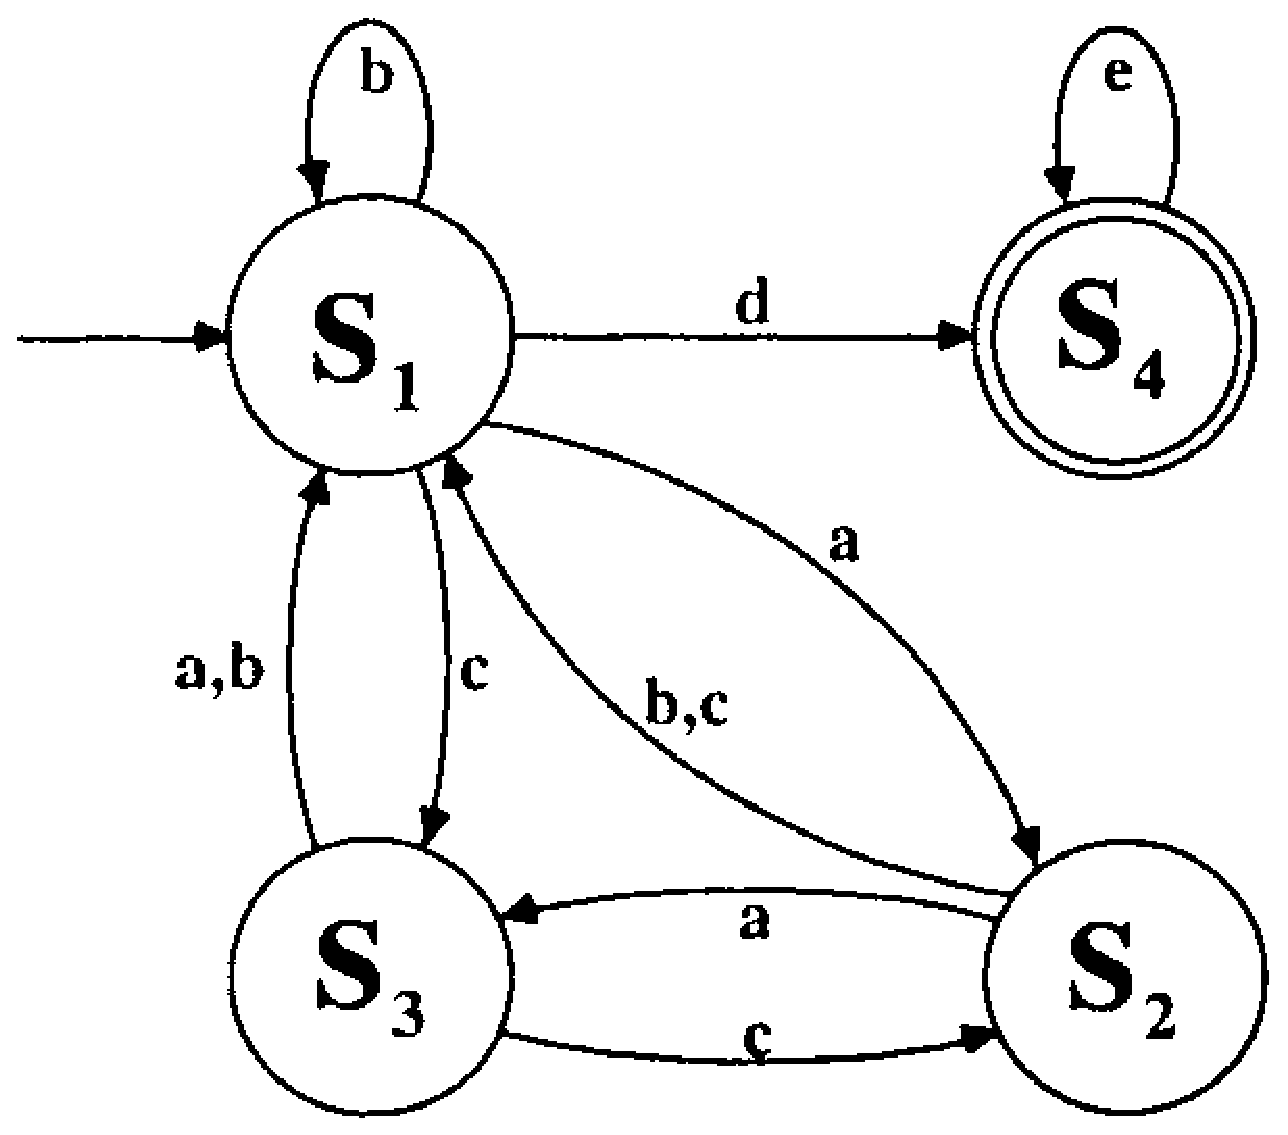
\epsfig{figure=ToFAfigures/fig6-8.eps,width=2.5in}}
\caption{The DFA discussed in Example 6.12}\label{fig-6.8}
\end{figure}

In general, the final coefficient and constant terms can always be interpreted
in this manner. In Example 6.11, the only way to reach a final state from $s_1$
and avoid having to return again to $s_1$ was to not leave in the first place;
this was reflected by the fact that $\hat{\hat{E}}_1 = \epsilon$.

\subsection*{Example 6.13}

% Figure 6.9
\begin{figure}
\centerline{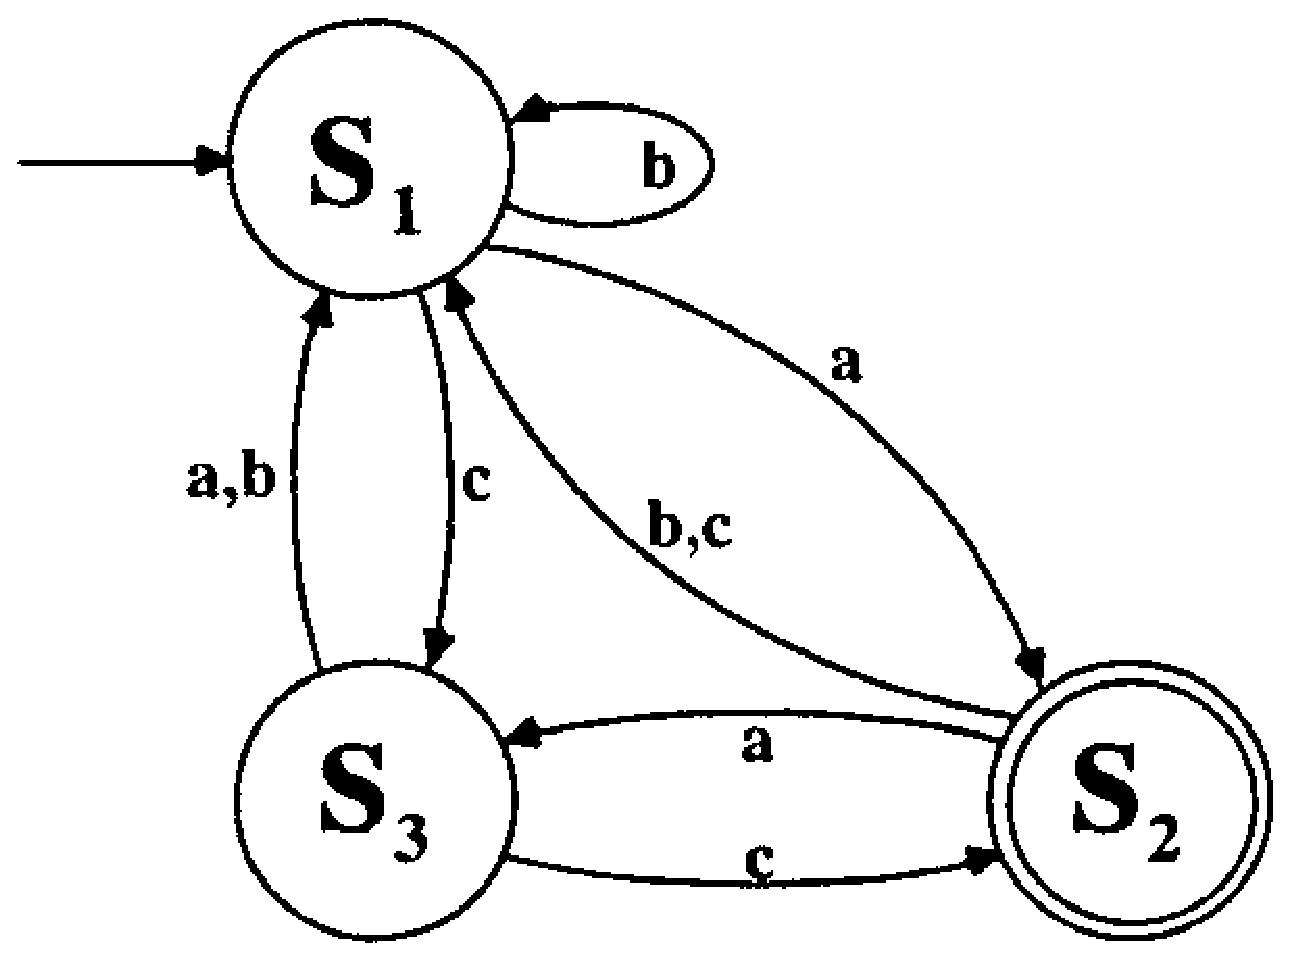
\epsfig{figure=ToFAfigures/fig6-9.eps,width=2.5in}}
\caption{The DFA discussed in Example 6.13}\label{fig-6.9}
\end{figure}

Consider the automaton illustrated in Figure \ref{fig-6.9}, which is identical to the
DFA in Example 6.11 except for the placement of the final state. Even though the
initial system of three equations is now different, we can expect
$\hat{\hat{A}}_{11}$ to compute to the same expression as before. Since
$\hat{\hat{E}}_1$ is supposed to represent all those strings that deposit you in
a final state from $s_1$ without ever returning to $s_1$, one should be able to
predict that the new final constant term will look like $\hat{\hat{E}}_1 =
\pmb{a}(\pmb{ac})^*\cup\pmb{c}(\pmb{ca})^*\pmb{c}$. An expression for the
language recognized by this automaton would then be given by

\begin{center}\begin{tabular}{r@{ = }l}
$X_1$ & $(\hat{\hat{A}}_{11})^*\hat{\hat{E}}_1$ \\
& $(\pmb{b}\cup\pmb{c}(\pmb{a}\cup\pmb{b})\cup(\pmb{a}\cup\pmb{cc})(\pmb{ac})^*
	((\pmb{b}\cup\pmb{c})\cup\pmb{a}(\pmb{a}\cup\pmb{b})))^*\cdot(\pmb{a}
	(\pmb{ac})^*\cup\pmb{c}(\pmb{ca})^*\pmb{c})$
\end{tabular}\end{center}

It may often be convenient to eliminate a variable other than the one that is
numerically last. This can be accomplished by appropriately renumbering the
unknowns and applying Theorem \ref{thm-6.2} to the new set of equations. For convenience,
we state an analog of Theorem \ref{thm-6.2} that allows the elimination of the $m^\text{th}$
unknown from a set of $n$ equations in $n$ unknowns. The following lemma agrees
with Theorem \ref{thm-6.2} if $m = n$.

% Lemma 6.3
\begin{lmm}\label{lmm-6.3}
Let $n$ and $m$ be positive integers and let $m \leq n$. Consider the system of
$n \geq 2$ equations in the unknowns $X_1,X_2,\ldots,X_n$, given by
\[ X_k = E_k \cup A_{k1}X_1 \cup A_{k2}X_2 \cup\cdots\cup A_{kn}X_n,\qquad
	\text{for }k = 1,2, \ldots , n \]
in which $(\forall i,j)(\lambda \notin A_{ij})$

The unknown $X_m$ can be eliminated from this system to form the following $n-1$
equations in the unknowns $X_1,X_2,\ldots,X_{m-1},X_{m+1},\ldots,X_n$.
\begin{center}\begin{tabular}{r@{ }l}
$X_k =$ & $\hat{E}_k \cup \hat{A}_{k1}X_1 \cup \hat{A}_{k2}X_2 \cup\ldots\cup
	\hat{A}_{k(m-1)}X_{m-1}\cup\hat{A}_{k(m+1)}X_{m+1}\cup\ldots\cup
	\hat{A}_{kn}X_n$, \\
& for $k = 1, 2,\ldots,m-1,m+1, \ldots ,n$
\end{tabular}\end{center}
where
\[ \hat{E}_i = E_i \cup (A_{im}\cdot A^*_{mm}\cdot E_m),\qquad\text{for all }
	i = 1,2, \ldots ,m-1,m+1, \ldots ,n \]
and
\[ \hat{A}_{ij} = A_{ij} \cup (A_{im}\cdot A^*_{mm}\cdot A_{mj}),\qquad
	\text{for all }i,j = 1,2, \ldots ,m-1,m+1, \ldots ,n \]
Furthermore, once the solution to the above $n-1$ equations is known, that
solution can be used to find the remaining unknown:
\begin{center}\begin{tabular}{r@{ }l}
$X_m =$ & $A^*_{mm} \cdot (E_m \cup A_{m1}X_1 \cup A_{m2}X_2 \cup\ldots\cup
	A_{m(m-1)}X_{m-1}$ \\
& $\cup\, A_{m(m+1)}X_{m+1}\cup\ldots\cup A_{mn}X_n)$
\end{tabular}\end{center}

\emph{Proof.} The proof follows from a renumbering of the equations given in
Theorem \ref{thm-6.2}.
\end{lmm}

% Figure 6.10
\begin{figure}
\centerline{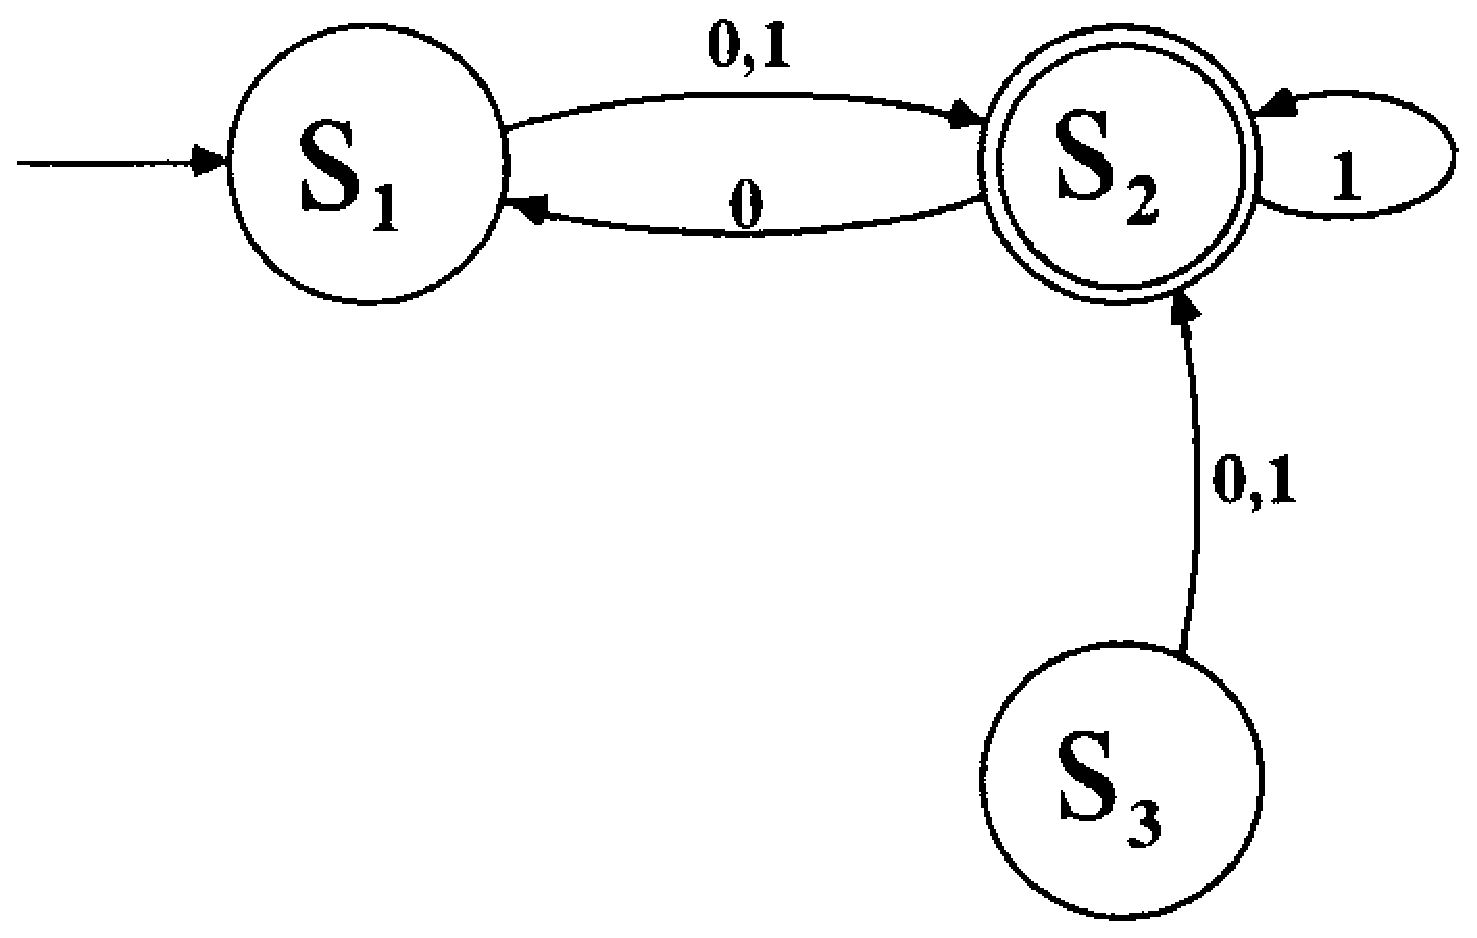
\epsfig{figure=ToFAfigures/fig6-10.eps,width=2.5in}}
\caption{The DFA discussed in Exercise 6.19}\label{fig-6.10}
\end{figure}

A significant reduction in the size of the expressions representing the
solutions can often be achieved by carefully choosing the order in which to
eliminate the unknowns. This situation can easily arise when solving language
equations that correspond to finite automata. For example, consider the DFA
illustrated in Figure \ref{fig-6.10}. The equations for this machine are given by
\begin{center}\begin{tabular}{r@{ = }l}
$X_1$ & $\emptyset\cup\emptyset X_1 \cup (\pmb{0}\cup\pmb{1})X_2\cup\emptyset
	X_3$ \\
$X_2$ & $\epsilon \cup \pmb{0} X_1 \cup \pmb{1}X_2 \cup \emptyset X_3$ \\
$X_3$ & $\emptyset\cup\emptyset X_1 \cup (\pmb{0}\cup\pmb{1})X_2\cup\emptyset
	X_3$
\end{tabular}\end{center}
Using Theorem \ref{thm-6.2} to methodically solve for $X_1$, $X_2$, and $X_3$ involves
eliminating $X_3$ and then eliminating $X_2$. Theorem \ref{thm-6.1} can then be used to
solve for $X_1$, and then the back-substitution rules can be employed to find
$X_2$ and $X_3$. The regular expressions found in this manner are quite complex.
A striking simplification can be made by eliminating $X_3$ and then eliminating
$X_1$ (instead of $X_2$) . The solution for $X_2$ is quite concise, which leads
to simple expressions for $X_1$ and $X_3$ during the back-substitution phase (see
Exercise 6.19).

Let $A=\langle\Sigma,\{s_1,s_2,\ldots,s_n\},s_1,\delta,F\rangle$ be a
deterministic finite automaton. We have seen that the relationships between the
terminal sets $T(A,s_i)$ described in Chapter \ref{ch-3} give rise to a system of
equations. Similarly, the initial sets $I(A,s_i)$ defined in Chapter \ref{ch-2} are also
interrelated. Recall that, for a state $s_i$, $I(A,s_i)$ is comprised of strings
that, when starting in the start state, lead to the state $s_i$. That is,
$I(A,s_i)=\{x\ \ |\ \DBAR(s_1,x) = s_i\}$. The equations we have discussed to this
point have been \emph{\Index{right linear}}; that is, the unknowns $X_i$ appear
to the right of their coefficients. The initial sets for an automaton are also
related by a system of equations, but these equations are \emph{\Index{left
linear}}; the unknowns $Y_i$ appear to the left of their coefficients. The
solution for sets of left-linear equations parallels that of right-linear
systems.

% Theorem 6.4
\begin{thm}\label{thm-6.4}
Let $n$ and $m$ be positive integers and let $m \leq n$. Consider the system of
$n \geq 2$ equations in the unknowns $Y_1,Y_2,\ldots,Y_n$ given by
\[ Y_k = I_k\cup Y_1B_{k1} \cup Y_2B_{k2} \cup\cdots\cup Y_nB_{kn},\qquad
	\text{for }k = 1,2,\ldots,n \]
in which $(\forall i,j)(\lambda \notin B_{ij})$.
\begin{enumerate}[a.]
\item The unknown $Y_m$ can be eliminated from this system to form the following
$n-1$ equations in the unknowns $Y_1,Y_2, \ldots , Y_{m-1},Y_{m+1},\ldots,Y_n$.
\[ Y_k = \hat{I}_k \cup Y_1\hat{B}_{k1} \cup Y_2\hat{B}_{k2} \cup\cdots\cup
	Y_{m-1}\hat{B}_{k(m-1)}\cup Y_{m+1}\hat{B}_{k(m+1)} \cup\cdots\cup
	Y_n\hat{B}_{kn}, \]
for $k = 1,2, \ldots ,m-1,m+1,\ldots, n$ \\
where
\[ \hat{I}_i=  I_i \cup(I_m \cdot B^*_{mm} \cdot B_{im}),\qquad\text{for all }
	i = 1,2,\ldots,m-1,m+1,\ldots,n \]
and
\[ \hat{B}_{ij} = B_{ij} \cup (B_{mj}\cdot B^*_{mm} \cdot B_{im}),\qquad
	\text{for all }i,j = 1,2,\ldots,m-1,m+1,\ldots,n \]

\item Once the solution to the above $n - 1$ equations is known, that solution
can be used to find the remaining unknown:
\begin{center}\begin{tabular}{r@{ }l}
$Y_m =$ & $(I_m \cup Y_1B_{m1} \cup Y_2B_{m2} \cup\cdots\cup Y_{m-1}B_{m(m-1)}$ \\
& $\cup\, Y_{m+1}B_{m(m+1)} \cup\cdots\cup Y_nB_{mn})\cdot B^*_{mm}$
\end{tabular}\end{center}

\item A single equation $Y_1=I_1 \cup Y_1B_{11}$ has the unique solution
$Y_1 = I_1B^*_{11}$.
\end{enumerate}

\emph{Proof.} The proof is essentially a mirror image of the proofs given in
Theorems \ref{thm-6.1} and \ref{thm-6.2}.
\end{thm}

% Lemma 6.4
\begin{lmm}\label{lmm-6.4}
Let $A=\langle\Sigma,\{s_1,s_2,\ldots,s_n\},S_0,\delta,F\rangle$ be an NDFA. For
each $i=1,2,\ldots,n$, let the initial set $I(A,s_i)=\{x\ |\ \DBAR(s_1,x) = s_i\}$
be denoted by $Y_i$. The unknowns $Y_1,Y_2,\ldots,Y_n$ satisfy a system of $n$
left-linear equations of the form
\[ Y_k = I_k \cup Y_1B_{k1} \cup Y_2B_{k2} \cup\cdots\cup Y_nB_{kn},\qquad
	\text{for }k = 1,2,\ldots,n \]
where the coefficients are given by
\begin{align*}
I_i = & \left\{ \begin{tabular}{ll}
			$\emptyset$ & if $s_i \notin S_0$ \\
			& \\
			$\epsilon$ & if $s_i \in S_0$
		 \end{tabular}\right. &
		 \text{for }i = 1,2,\ldots,n \\
\intertext{and}
B_{ij} = & \bigcup\limits_{\pmb{a}\,\in\,\Sigma\,\wedge\,s_i\,\in\,\delta(s_j,
	\pmb{a})} \pmb{a} & \text{for }i,j=1,2, \ldots ,n
\end{align*}

\emph{Proof.} See the exercises.
\end{lmm}

In contrast to Theorem \ref{thm-6.3}, where $A_{ij}$ represented the set of all letters
that causes a transition from state $s_i$ to state $s_j$, $B_{ij}$ represents
the set of all letters that causes a transition from state $s_j$ to state $s_i$.
That is, $B_{ij} = A_{ji}$. In the definition in Theorem \ref{thm-6.3}, $E_i$ represented
the set of all strings of length zero that can reach final states from $s_i$.
Compare this with the definition of $I_i$ above, which represents the set of all
strings of length zero that can reach $s_i$ from a start state.

\section{FAD Languages As Regular Sets; Closure Properties}\label{sec-6.4}

The technique outlined by Theorems \ref{thm-6.1}, \ref{thm-6.2}, and \ref{thm-6.3}
provide the second half of the correspondence between regular sets and FAD
languages. As a consequence, regular expressions and automata characterize
exactly the same class of languages.

% Corollary 6.2
\begin{cor}\label{cor-6.2}
Let $\Sigma$ be an alphabet. Then $\DSIG \subseteq \RSIG$.

\emph{Proof.} The proof follows immediately from Theorem \ref{thm-6.3}.
\end{cor}

% Theorem 6.5
\begin{thm}\label{thm-6.5}\index{equivalent!regular expressions}
{\bf \Index{Kleene's Theorem}}. Let $\Sigma$ be an alphabet. Then $\RSIG = \DSIG$.

\emph{Proof.} The proof follows immediately from Corollaries 6.1 and 6.2.
\end{thm}

Thus the terms \emph{FAD language} and \emph{regular set} can be used
interchangeably, since languages accepted by finite automata can be described by
regular expressions, and vice versa. Such languages are often referred to as
\emph{\Index{regular language}s}. The correspondence will allow, for example,
the pumping lemma to be invoked to justify that certain languages cannot be
represented by any regular expression.

\RSIG\ is therefore closed under every operator for which \DSIG\ is closed. We
have now seen two representations for FAD languages, and a third will be
presented in Chapter \ref{ch-8}. Since there are effective algorithms for switching from
one representation to another, we may use whichever vehicle is most convenient
to describe a language or prove properties about regular languages. For example,
we may use whichever concept best lends itself to the proof of closure
properties. The justification that \RSIG\ is closed under union follows
immediately from Definition \ref{dfn-6.1}; much more effort was required in Chapter \ref{ch-5} to
prove that the union of two languages represented by DFAs could be represented
by another DFA. On the other hand, attempting to justify closure under
complementation by using regular expressions is an exercise in frustration. We
will now see that closure under \emph{substitution} is conveniently
proved via regular expressions.

A substitution is similar to a language homomorphism (Definition \ref{dfn-5.8}), in
which letters were replaced by single words. Substitutions will denote the
methodical replacement of the individual letters within a regular expression
with \emph{sets} of words. The only restriction on these sets is that they must
also be regular expressions, though not necessarily over the same alphabet.

% Definition 6.5
\begin{dfn}\label{dfn-6.5}\index{substitution!regular set}
Let $\Sigma=\{\pmb{a}_1,\pmb{a}_2,\ldots,\pmb{a}_m\}$ be an alphabet and let
$\Gamma$ be a second alphabet. Given regular expressions $R_1,R_2,\ldots,R_m$
over $\Gamma$, define a \emph{\Index{regular set substitution}} $s$$:\Sigma
\rightarrow \wp(\Gamma^*)$ by $s(\pmb{a}_i) = R_i$ for each $i=1,2,\ldots,m$,
which can be extended to $\overline{s}:\ \Sigma^* \rightarrow \wp(\Gamma^*)$ by
\[ \overline{s}(\lambda) = \epsilon \]
and
\[ (\forall\pmb{a}\in\Sigma)(\forall x \in\Sigma^*)(\overline{s}(\pmb{a}\cdot x)
	= s(\pmb{a})\cdot \overline{s}(x)) \]
$\overline{s}$ can be further extended to operate on a language $L \subseteq
\Sigma^*$ by defining
\[ \overline{s}(L) = \bigcup\limits_{z\,\in\, L} \overline{s}(z) \]
In this last context, $\overline{s}:\ \wp(\Sigma^*) \rightarrow \wp(\Gamma^*)$.
\end{dfn}

\subsection*{Example 6.14}

Let $\Sigma=\{\pmb{0}\}$ and $\Gamma=\{\pmb{a},\pmb{b}\}$. Define $s(\pmb{0}) =
(\pmb{a}\cup\pmb{b})\cdot(\pmb{a}\cup\pmb{b})$. From the recursive definition,
$\overline{s}(\pmb{00}) = (\pmb{a}\cup\pmb{b})\cdot(\pmb{a}\cup\pmb{b})\cdot
(\pmb{a}\cup\pmb{b})\cdot(\pmb{a}\cup\pmb{b})$. Furthermore, the language
$\overline{s}(\pmb{0}^*)$ represents all even-length strings over $\{\pmb{a},
\pmb{b}\}$.

The definition of $\overline{s}(L)$ for a language $L$ allows the domain of the
substitution to be extended all the way to $\overline{s}$$: \wp(\Sigma^*) \rightarrow \wp
(\Gamma^*)$. It can be proven that the image of \RSIG\ under $\overline{s}$ is
contained in $\mathfrak{R}_{\Gamma}$ (see the exercises); however, the image of
\NSIG\ under $\overline{s}$ is not completely contained in $\mathfrak{N}_{\Gamma}$

In Example 6.14, the language $\pmb{0}^*$ was regular and so was its image under
$\overline{s}$. %Neither of the sets described in the second example were regular.
It is possible to start with a nonregular set and define a substitution that
produces a regular set (see Lemma \ref{lmm-6.5}), but it is impossible for the image of a
regular set to avoid being regular, as shown by the next theorem.

% Theorem 6.6
\begin{thm}\label{thm-6.6}\index{closure!under substitution}
Let $\Sigma$ be an alphabet, and let $s:\ \Sigma \rightarrow \wp(\Sigma^*)$ be a
substitution. Then \RSIG\ is closed under $\overline{s}$.

\emph{Proof.} Choose an arbitrary regular expression $R$ over $\Sigma$. We must
show that $\overline{s}(R)$ represents a regular set. $R$ is an expression made
up of the letters in $\Sigma$ and the characters $(,),\cup$, and $^*$. Form the
new expression $R'$ by replacing each letter $\pmb{a}$ by $s(\pmb{a})$. $R'$ is
then clearly another regular expression over $\Sigma$. In fact, it can be shown
that $R'$ represents exactly the words in $\overline{s}(R)$; this is formally
accomplished by inducting on the number of operators in the expression $R$. To
prove this, one must argue that this substitution correspondence is preserved by
each of the six rules defining regular expressions. The basis step of the
induction involves all regular expressions with zero operators, that is, those
defined by the first three rules for generating a regular expression.
\begin{enumerate}[i.]
\item The substitution corresponding to any single letter $\pmb{a}_i$ is a
regular expression corresponding to $\overline{s}(\pmb{a}_i)$, since, by
definition of $\overline{s}$, $\overline{s}(\pmb{a}_i) = s(\pmb{a}_i)$.
\item The substitution corresponding to $\emptyset$ is a regular expression
corresponding to $\overline{s}(\emptyset)$, since, by definition of
$\overline{s}$, $\overline{s}(\emptyset) = \emptyset$.
\item The substitution corresponding to $\epsilon$ is a regular expression
corresponding to $\overline{s}(\lambda)$, since, by definition of $\overline{s}$,
$\overline{s}(\lambda) = \epsilon$.
\end{enumerate}
The inductive step requires an argument that the correspondence is preserved
whenever another of the three operators is introduced to form a more complex
expression. These assertions involve the final three rules for generating
regular expressions.
\begin{enumerate}[i.]
\setcounter{enumi}{3}
\item If $R_1$ and $R_2$ are regular expressions, then the substitution
corresponding to $(R_1\cdot R_2)$ is a regular expression representing the
concatenation of the two corresponding substitutions. That is, $\overline{s}(R_1
\cdot R_2) = \overline{s}(R_1)\cdot\overline{s}(R_2)$.
\item If $R_1$ and $R_2$ are regular expressions, then the substitution
corresponding to $(R_1 \cup R_2)$ is a regular expression representing
$\overline{s}(R_1)\cup\overline{s}(R_2)$.
\item If $R_1$ is a regular expression, then the substitution corresponding to
$(R_1)^*$ is a regular expression representing $(\overline{s}(R_1))^*$.
\end{enumerate}
Each of these three assertions follows immediately from the definition of
substitution and is left as an exercise. The inductive step guarantees that
the substitution correspondence is preserved in any regular expression $R$,
regardless of the number of operators in $R$. Consequently, $R'$ is indeed a
regular expression denoting $\overline{s}(R)$, and \RSIG\ is therefore closed
under $\overline{s}$.
\end{thm}

The analogous result does \emph{not} always hold for the nonregular sets.
% Lemma 6.5
\begin{lmm}\label{lmm-6.5}
Let $\Sigma$ be an alphabet.
\begin{enumerate}[a.]
\item There are examples of regular set substitutions $s:\ \Sigma \rightarrow
	\wp(\Sigma^*)$ for which \NSIG\ is not closed under $\overline{s}$.
\item There are examples of regular set substitutions $t:\ \Sigma \rightarrow
	\wp(\Sigma^*)$ for which \NSIG\ is closed under $\overline{t}$.
\end{enumerate}

\emph{Proof.} (a) \NSIG\ is \emph{not} closed under some substitutions. Let
$\Sigma=\{\pmb{a},\pmb{b}\}$ and define $s(\pmb{a})=(\pmb{a}\cup\pmb{b})$ and
$s(\pmb{b})=(\pmb{a}\cup\pmb{b})$. The image of the nonregular set
\[ L = \{x\ | \  |x|_{\pmb{a}} = |x|_{\pmb{b}}\} \]
is the set of even-length words, which \emph{is} regular. Thus $L \in \NSIG$ but
$\overline{s}(L) \notin \NSIG$.

(b) \NSIG\ \emph{is} closed under some substitutions. Some substitutions do
preserve nonregularity (such as the identity substitution $i$, since for any
language $L$, $\overline{i}(L) = L$). In this case, $(\forall L)(L \in \NSIG
\Rightarrow \overline{i}(L)\in \NSIG)$ and therefore \NSIG\ is closed under
$\overline{i}$.
\end{lmm}
Note that a substitution in which each $R_i$ is a single string then conforms to
Definition \ref{dfn-5.8} and represents a language homomorphism.

% Corollary 6.3
\begin{cor}\label{cor-6.3}\index{closure!under language homomorphism}
Let $\Sigma$ be an alphabet, and let $\psi:\ \Sigma \rightarrow \Sigma^*$ be a
language homomorphism. Then \RSIG\ is closed under \PBAR.

\emph{Proof.} The proof follows immediately from Theorem \ref{thm-6.6}, since a language
homomorphism is a special type of substitution.
\end{cor}

As in Chapter \ref{ch-5}, this result can also be proved by successfully modifying an
appropriate DFA, showing that $\DSIG ( = \RSIG)$ is closed under language
homomorphism. It is likewise possible to use machine constructs to show that
\DSIG\ is closed under substitution, but this becomes much more complex than the
argument given for Theorem \ref{thm-6.6}. A third characterization of regular languages
will be presented in Chapter \ref{ch-8}, affording a choice of three distinct avenues for
proving closure properties of \RSIG.

\section*{Exercises}
\begin{enumerate}[{6.}1.]
\item Let $\Sigma=\{\pmb{a},\pmb{b}\}$. Give (if possible) a regular expression
that describes the set of all even-length words in $\Sigma^*$.

\item Let $\Sigma=\{\pmb{a},\pmb{b}\}$. Give (if possible) a regular expression
that describes the set of all words $x$ in $\Sigma^*$ for which $|x| \geq 2$.

\item Let $\Sigma=\{\pmb{a},\pmb{b}\}$. Give (if possible) a regular expression
that describes the set of all words $x$ in $\Sigma^*$ for which $|x|_{\pmb{a}} =
|x|_{\pmb{b}}$.

\item Let $\Sigma=\{\pmb{a},\pmb{b},\pmb{c}\}$. Give a regular expression that
describes the set of all odd-length words in $\Sigma^*$ that do not end in $\pmb{b}$.

\item Let $\Sigma=\{\pmb{a},\pmb{b},\pmb{c}\}$. Give a regular expression that
describes the set of all words in $\Sigma^*$ that do \emph{not} contain
two consecutive $\pmb{c}$s. 

\item Let $\Sigma=\{\pmb{a},\pmb{b},\pmb{c}\}$. Give a regular expression that
describes the set of all words in $\Sigma^*$ that \emph{do} contain
two consecutive $\pmb{c}$s.

\item Let $\Sigma=\{\pmb{a},\pmb{b},\pmb{c}\}$. Give a regular expression that
describes the set of all words in $\Sigma^*$ that do \emph{not} contain
\emph{any} $\pmb{c}$s.

\item Let $\Sigma=\{\pmb{0},\pmb{1}\}$. Give, if possible, regular expressions
that will describe each of the following languages. Try to write these directly
from the descriptions (that is, avoid relying on the nature of the corresponding
automata).
\begin{enumerate}
\item $L_1 = \{x\ |\ \ \ |x| \bmod{3} = 2\}$
\item $L_2 = \Sigma^* - \{w\ |\ \exists n \geq 1 \ni w = a_1\ldots a_n \wedge a_n
	= \pmb{1}\}$
\item $L_3 = \{y\ |\ \ \ |y|_{\pmb{0}} > |y|_{\pmb{1}}\}$
\end{enumerate}

\item Let $\Sigma=\{\pmb{a},\pmb{b},\pmb{c}\}$. Give, if possible, regular
expressions that will describe each of the following languages. Try to write
these directly from the descriptions (that is, avoid relying on the nature of
the corresponding automata).
\begin{enumerate}
\item $L_1 = \{x\ |\ \ \ (|x|_{\pmb{a}}$ is odd$)\wedge(|x|_{\pmb{b}}$ is even$)\}$
\item $L_2 = \{y\ |\ \ \ (|y|_{\pmb{c}}$ is even$)\vee(|y|_{\pmb{b}}$ is odd$)\}$
\item $L_3 = \{z\ |\ \ \ (|z|_{\pmb{a}}$ is even$)\}$
\item $L_4 = \{z\ |\ \ \ |z|_{\pmb{c}}$ is a prime number$\}$
\item $L_5 = \{x\ |\ \pmb{abc}$ is a substring of $x\}$
\item $L_6 = \{x\ |\ \pmb{acaba}$ is a substring of $x\}$
\item $L_7 = \{x \in \{\pmb{a},\pmb{b},\pmb{c}\}^*|\ \ \ |x|_{\pmb{a}} \equiv 0
	\bmod{3}\}$
\end{enumerate}

\item Let $\Sigma=\{\pmb{a},\pmb{b},\pmb{d}\}$. Give a regular expression that
will describe
\[ \Psi = \{x \in \Sigma^*\ |\ (x\text{ begins with }\pmb{d})\vee(x\text{ contains
	two consecutive $\pmb{b}$s})\}. \]

\item Let $\Sigma=\{\pmb{a},\pmb{b},\pmb{c}\}$. Give a regular expression that
will describe
\[ \Phi = \{x \in \Sigma^*\ |\ \text{every $\pmb{b}$ in $x$ is immediately followed
	by }\pmb{c}\}. \]

\item Let $\Sigma=\{\pmb{0},\pmb{1},\pmb{2},\pmb{3},\pmb{4},\pmb{5},\pmb{6},
\pmb{7},\pmb{8},\pmb{9}\}$. Give a regular expression that will describe
\begin{center}\begin{tabular}{r@{ = }l}
$\Gamma$ & $\{x \in \Sigma^*|\ $the number represented by $x$ is evenly
	divisible by $3\}$ \\
& $\{\lambda,\pmb{0},\pmb{00},\pmb{000},\ldots,\pmb{3},\pmb{03},\pmb{003},
	\ldots,\pmb{6},\pmb{9},\pmb{12},\pmb{15},\ldots\}$.
\end{tabular}\end{center}

\item Let $\Sigma = \{\pmb{0},\pmb{1},\pmb{2},\pmb{3},\pmb{4},\pmb{5},\pmb{6},
\pmb{7},\pmb{8},\pmb{9}\}$. Give a regular expression that will describe
\[ K = \{x \in \Sigma^*|\ \text{the number represented by $x$ is evenly divisible
	by }5\}. \]

\item Use the \emph{exact} constructs given in the theorems of Chapter \ref{ch-5} to build a
NDFA that accepts $\pmb{b}\cup\pmb{a}^*\pmb{c}$ (refer to Examples 6.4,
6.5, and 6.6). Do \emph{not} simplify your answer.

\item Give examples of sets that demonstrate the following inequalities listed
in Lemma \ref{lmm-6.1}:
\begin{enumerate}
\item $R_1 \cup \epsilon \neq R_1$
\item $R_1 \cdot R_2 \not= R_2 \cdot R_1$
\item $R_1 \cdot R_1 \not= R_1$
\item $R_1 \cup (R_2 \cdot R_3) \not= (R_1 \cup R_2)\cdot(R_1 \cup R_3)$
\item $(R_1 \cdot R_2)^* \not= (R^*_1 \cdot R^*_2)^*$
\item $(R_1 \cdot R_2)^* \not= (R^*_1 \cup R^*_2)^*$
\end{enumerate}
Find other examples of sets that show the following expressions may be equal
under some conditions:
\begin{enumerate}
\setcounter{enumii}{6}
\item $R_1 \cup \epsilon = R_1$
\item $R_1 \cdot R_2 = R_2 \cdot R_1\qquad$ (even if $\lambda \neq R_1 \neq R_2 \neq \lambda$)
\item $R_1 \cdot R_1 = R_1$
\item $R_1 \cup (R_2 \cdot R_3) = (R_1 \cup R_2)\cdot(R_1 \cup R_3)\qquad$
	(even if $R_1 \not= R_2 \not= R_3 \not= R_1$)
\item $(R_1 \cdot R_2)^* = (R^*_1 \cdot R^*_2)^*\qquad$
(even if $\lambda \neq R_1 \neq R_2 \neq \lambda$)
\item $(R_1 \cdot R_2)^* = (R^*_1 \cup R^*_2)^*\qquad$
(even if $\lambda \neq R_1 \neq R_2 \neq \lambda$)
\end{enumerate}

\item Prove the equalities listed in Lemma \ref{lmm-6.1}.

\item \begin{enumerate}
\item Consider Theorem \ref{thm-6.1}. Find examples of sets $A$ and $E$ that will show
that $A^*\!\!\cdot E$ is not a unique solution if $\lambda \in A$.
\item Find examples of sets $A$ and $E$ that will show that $A^*\!\!\cdot E$ can be
the unique solution even if $\lambda \in A$.
\end{enumerate}

\item Solve the following set of language equations for $X_0$ \emph{and} $X_1$
over $\{\pmb{0},\pmb{1}\}^*$:
\begin{center}\begin{tabular}{r@{ = }l}
$X_0$ & $(\pmb{0}\cup\pmb{1})X_1$ \\
$X_1$ & $\epsilon\cup\pmb{1}X_0\cup\pmb{0}X_1$
\end{tabular}\end{center}
Do you see any relation between these equations and the DFA $A$ in Example 3.4?

\item \begin{enumerate}
\item Solve the following set of language equations for $X_1$, $X_2$, \emph{and} $X_3$
by eliminating $X_3$ and then eliminating $X_2$. Solve for $X_1$ and then
back-substitute to find $X_2$ and $X_3$. Note that these equations arise from
the automaton in Figure \ref{fig-6.10}.
\begin{center}\begin{tabular}{r@{ = }l@{ $\cup$ }l}
$X_1$ & $\emptyset\cup\emptyset X_1 \cup (\pmb{0}\cup\pmb{1})X_2$ & $\emptyset
	X_3$ \\
$X_2$ & $\epsilon\cup\pmb{0}X_1\cup\pmb{1}X_2$ & $\emptyset X_3$ \\
$X_3$ & $\emptyset\cup\emptyset X_1\cup(\pmb{0}\cup\pmb{1})X_2$ & $\emptyset X_3$
\end{tabular}\end{center}
\item Rework part (a) by eliminating $X_3$ and then eliminating $X_1$ (instead
	of $X_2$).
\item How does the solution in part (b) compare to the solution in part (a)? Is
one more concise? Are they equivalent?
\end{enumerate}

\item Prove Lemma \ref{lmm-6.2}. [\emph{Hint:} Let $P(m)$ be the statement that ``Every
regular expression $R$ with $m$ or fewer operators represents a regular set that
is FAD,'' and induct on $m$]

\item Let $\Sigma=\{\pmb{a},\pmb{b},\pmb{c}\}$. Find all solutions to the
language equation $X=X\cup\{\pmb{b}\}$.

\item Prove that, for any languages $A$ and $E$, $A^*E=E\cup A\cdot(A^*E)$.

\item Give a regular expression that describes the \emph{intersection} of
the regular sets $(\pmb{ab}\cup\pmb{b})^*\pmb{a}$ and $(\pmb{ba}\cup\pmb{a})^*$.

\item Develop an algorithm that, when applied to two regular expressions, will
generate an expression describing their intersection.

\item Verify by direct substitution that $X_1=(\pmb{a}\cup\pmb{bb})^*$ and $X_2 =
\pmb{b}\cdot(\pmb{a}\cup\pmb{bb})^*$ is a solution to
\begin{center}\begin{tabular}{r@{ = }l}
$X_1$ & $\epsilon\cup\pmb{a}\cdot X_1\cup\pmb{b}\cdot X_2$ \\
$X_2$ & $\emptyset\cup\pmb{b}\cdot X_1 \cup\emptyset\cdot X_2$
\end{tabular}\end{center}

\item \begin{enumerate}
\item Find $L(D)$ for the machine $D$ described in Example 6.10.
\item Generalize your technique: For a machine $A$ with start states $s_{i_1},\ s_{i_2},
\ldots, s_{i_m},\ L(A)$ is given by \line(1,0){50}?
\end{enumerate}

\item Let $\Sigma=\{\pmb{a},\pmb{b}\}$. Give a regular expression that will
describe the \emph{complement }of the regular set\linebreak$(\pmb{ab}\cup\pmb{b})^*\pmb{a}$.

\item Develop an algorithm that, when applied to a regular expression, will
generate an expression describing the complement.

\item Let $\Sigma=\{\pmb{a},\pmb{b},\pmb{c}\}$. Define $E(L)=\{z\ |\ (\exists y
\in \Sigma^+)(\exists x \in L)z = yx\}$. Use the regular expression concepts
given in this chapter to argue that \RSIG\ is closed under the operator $E$
(that is, don't build a new automaton; build a new regular expression from the
old expression).

\item Let $\Sigma=\{\pmb{a},\pmb{b},\pmb{c}\}$. Define $B(L)=\{z\ |\ (\exists x
\in L)(\exists y \in \Sigma^*)z = xy\}$. Use the regular expression concepts
given in this chapter to argue that \RSIG\ is closed under the operator $B$
(that is, don't build a new automaton; build a new regular expression from the
old expression).

\item Let $\Sigma=\{\pmb{a},\pmb{b},\pmb{c}\}$. Define $M(L)=\{z\ |\ (\exists x
\in L)(\exists y \in\Sigma^+)z = xy\}$. Use the regular expression concepts
given in this chapter to argue that \RSIG\ is closed under the operator $M$
(that is, don't build a new automaton; build a new regular expression from the
old expression).

\item \begin{enumerate}
\item Let $\Sigma=\{\pmb{a},\pmb{b},\pmb{c}\}$. Show that there does \emph{not}
exist a \emph{unique} solution to the following set of language equations:
\begin{center}\begin{tabular}{r@{ = }l}
$X_1$ & $\pmb{b}\cup\epsilon\cdot X_1\cup\pmb{a}\cdot X_2$ \\
$X_2$ & $\pmb{c}\cup\emptyset\cdot X_1 \cup\epsilon\cdot X_2$
\end{tabular}\end{center}
\item Does this contradict Theorem \ref{thm-6.2}? Explain.
\end{enumerate}

\item Solve the following set of language equations for $X_0$ \emph{and} $X_1$ over
$\{\pmb{0},\pmb{1}\}^*$:
\begin{center}\begin{tabular}{r@{ = }l@{ $\cup$ }l@{ $\cup$ }l}
$X_0$ & $\pmb{0}^*\pmb{1}$ & $(\pmb{10})^*X_0$ & $\pmb{0}(\pmb{0}\cup\pmb{1})X_1$ \\
$X_1$ & $\epsilon$ & $\pmb{1}^*\pmb{01} X_0$ & $\qquad\ \ \ \pmb{0}X_1$
\end{tabular}\end{center}

\item Let $\Sigma=\{\pmb{a},\pmb{b},\pmb{c}\}$.
\begin{enumerate}
\item Give a regular expression that describes the set of all words in $\Sigma^*$
that end with $\pmb{c}$ and for which $\pmb{aa}$, $\pmb{bb}$, and $\pmb{cc}$ never
appear as substrings.
\item Give a regular expression that describes the set of all words in $\Sigma^*$
that begin with $\pmb{c}$ and for which $\pmb{aa}$, $\pmb{bb}$, and $\pmb{cc}$ never
appear as substrings.
\end{enumerate}

\item Let $\Sigma=\{\pmb{a},\pmb{b},\pmb{c}\}$.
\begin{enumerate}
\item Give a regular expression that describes the set of all words in $\Sigma^*$
that contain no more than two $\pmb{c}$s.
\item Give a regular expression that describes the set of all words in $\Sigma^*$
that do not have exactly one $\pmb{c}$.
\end{enumerate}

\item Recall that the reverse of a word $x$, written $x^r$, is the word written
backward. The reverse of a language is likewise given by $L^r=\{x^r\ |\ x \in L\}$.
Let $\Sigma=\{\pmb{a},\pmb{b},\pmb{c}\}$.
\begin{enumerate}
\item Note that $(R_1 \cup R_2)^r = (R^r_1 \cup R^r_2)$ for any regular sets $R_1$
and $R_2$. Give similar equivalences for each of the rules in Definition \ref{dfn-6.1}.
\item If $L$ were represented by a regular expression, explain how to generate a
regular expression representing $L^r$ (compare with the technique used in the
proof of Theorem \ref{thm-6.6}).
\item Prove part (b) by inducting on the number of operators in the expression.
\item Use parts (a), (b), and (c) to argue that \RSIG\ is closed under the
operator $r$.
\end{enumerate}

\item Complete the details of the proof of Theorem \ref{thm-6.4}.

\item Let $\Sigma=\{\pmb{a},\pmb{b},\pmb{c}\}$.
\begin{enumerate}
\item Give a regular expression that describes the set of all words in $\Sigma^*$
for which no $\pmb{b}$ is immediately preceded by $\pmb{a}$.
\item Give a regular expression that describes the set of all words in $\Sigma^*$
that contain exactly two $\pmb{c}$s and for which no $\pmb{b}$ is immediately
preceded by $\pmb{a}$.
\end{enumerate}

\item Let $\Sigma=\{\pmb{a},\pmb{b},\pmb{c}\}$.
\begin{enumerate}
\item Give a regular expression that describes the set of all words in $\Sigma^*$
for which no $\pmb{b}$ is immediately preceded by $\pmb{c}$.
\item Give a regular expression that describes the set of all words in $\Sigma^*$
that contain exactly one $\pmb{c}$ and for which no $\pmb{b}$ is immediately
preceded by $\pmb{c}$.
\end{enumerate}

\item \begin{enumerate}
\item Use Theorem \ref{thm-6.3} to write the two right-linear equations in two unknowns
corresponding to the NDFA given in Figure \ref{fig-6.11}.
% Figure 6.11
\begin{figure}
\centerline{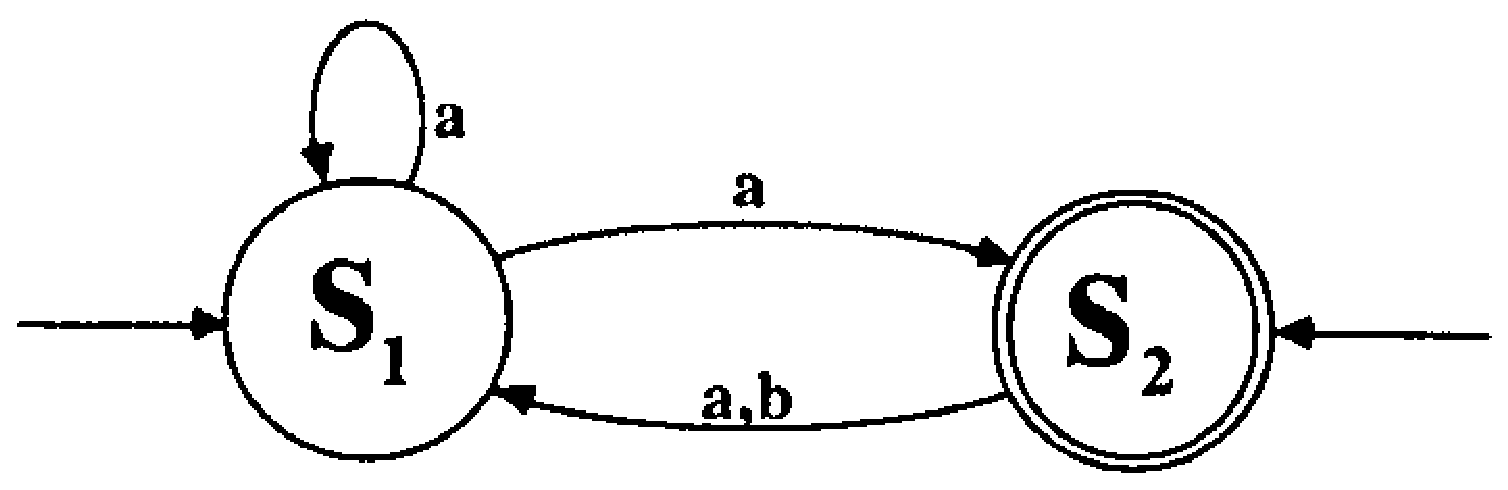
\epsfig{figure=ToFAfigures/fig6-11.eps,width=2.5in}}
\caption{The NDFA for Exercise 6.40}\label{fig-6.11}
\end{figure}
\item Solve these equations for both unknowns.
\item Give a regular expression that corresponds to the language accepted by
this NDFA.
\item Rework the problem with two left-linear equations.
\end{enumerate}

\item \begin{enumerate}
\item Use Theorem \ref{thm-6.3} to write the four right-linear equations in four unknowns
corresponding to the NDFA given in Figure \ref{fig-6.12}.
% Figure 6.12
\begin{figure}
\centerline{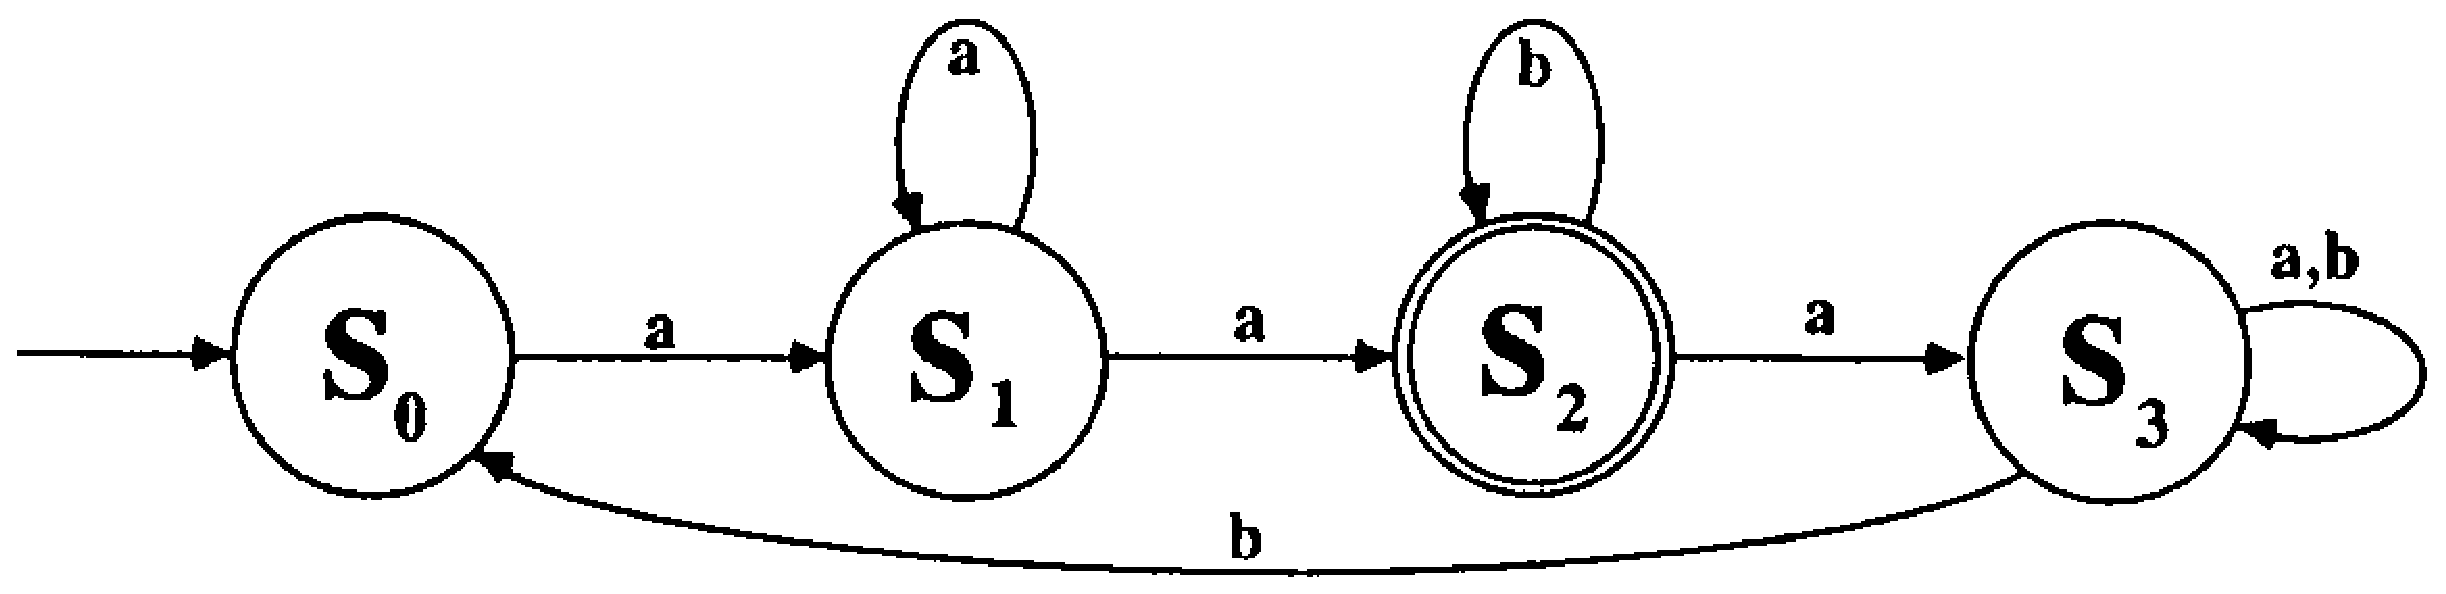
\epsfig{figure=ToFAfigures/fig6-12.eps,width=4.5in}}
\caption{The automaton for Exercise 6.41}\label{fig-6.12}
\end{figure}
\item Solve these equations for all four unknowns.
\item Give a regular expression that corresponds to the language accepted by
this NDFA.
\item Rework the problem with four left-linear equations.
\end{enumerate}

\item \begin{enumerate}
\item Use Theorem \ref{thm-6.3} to write the seven right-linear equations in seven
unknowns corresponding to the NDFA given in Figure \ref{fig-6.13}.
% Figure 6.13
\begin{figure}
\centerline{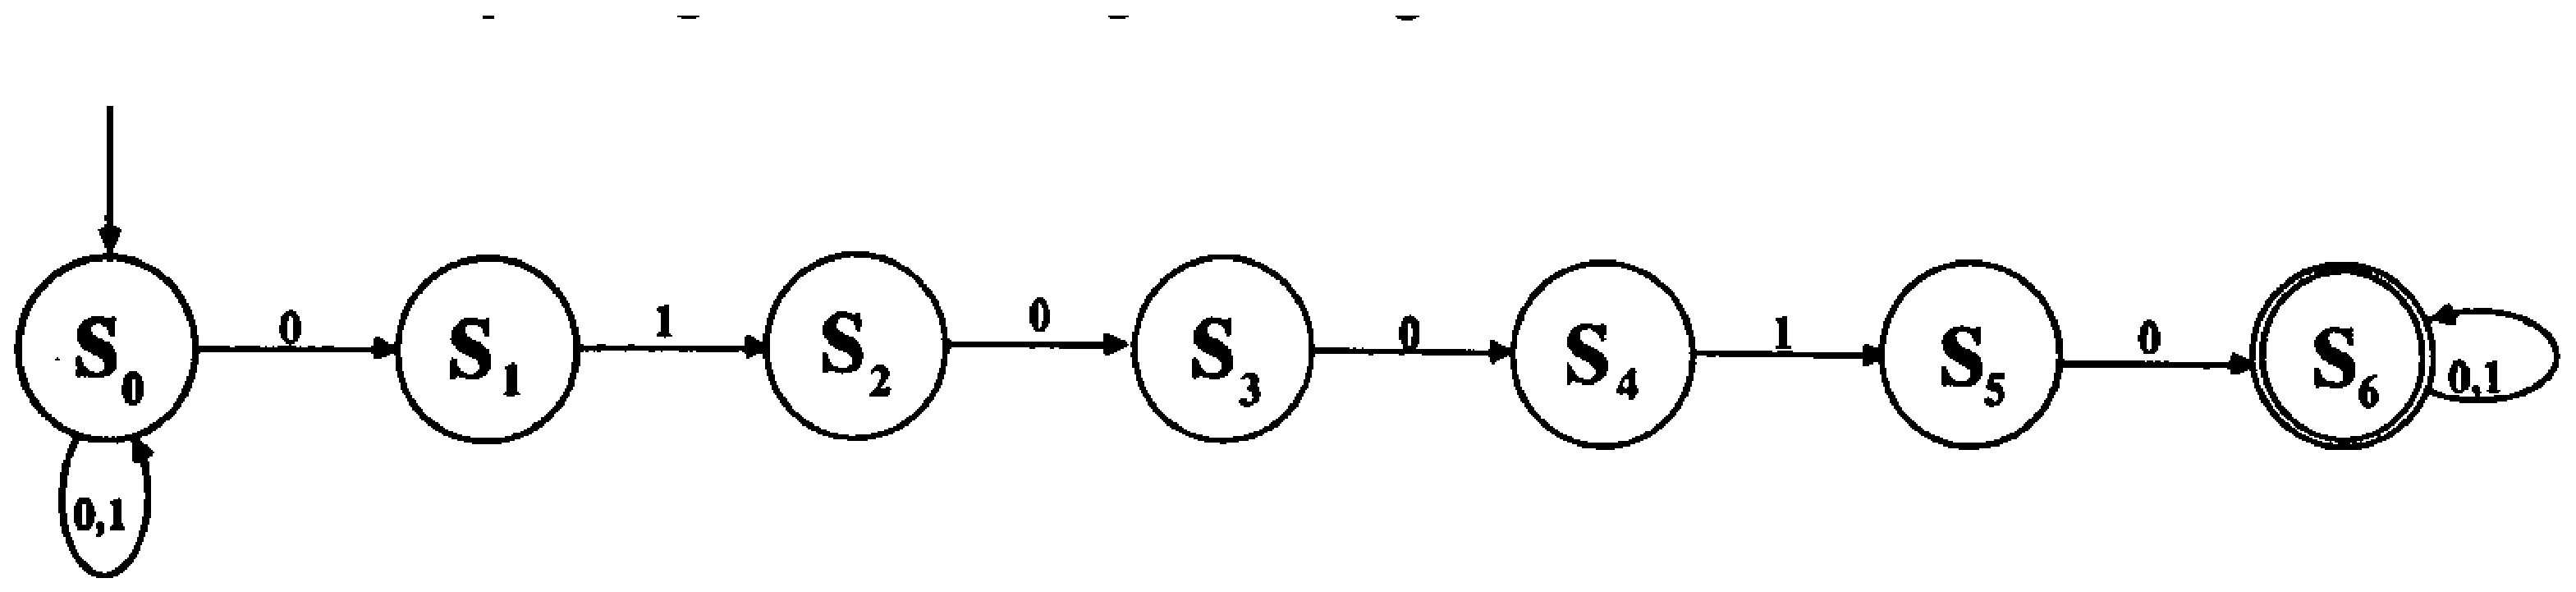
\epsfig{figure=ToFAfigures/fig6-13.eps,width=6.5in}}
\caption{The NDFA for Exercise 6.42}\label{fig-6.13}
\end{figure}
\item Solve these equations for all seven unknowns. \emph{Hint:} Make use of the
simple nature of these equations to eliminate variables without appealing to
Theorem \ref{thm-6.2}.
\item Give a regular expression that corresponds to the language accepted by
this NDFA.
\item Rework the problem with seven left-linear equations.
\end{enumerate}

\item Prove that for \emph{any} languages $A$, $E$, and $Y$, if $E \subseteq Y$,
then $A \cdot E \subseteq A \cdot Y$.

\item Let $\Sigma$ be an alphabet, and let $s:\ \Sigma \rightarrow \Gamma^*$ be
a substitution.
\begin{enumerate}
\item Prove that the image of \RSIG\ under $\overline{s}$ is contained in $\mathfrak{R}_{\Gamma}$.
\item Give an example to show that the image of \NSIG under $\overline{s}$ need
not be completely contained in $\mathfrak{N}_{\Gamma}$.
\end{enumerate}

\item Give a detailed proof of Lemma \ref{lmm-6.3}.

\item Let $\Sigma=\{\pmb{a},\pmb{b}\}$ and $\Xi=\{x \in \Sigma^*|\ x$ contains (at
least) two consecutive $\pmb{b}$s $\wedge x$ does \emph{not} contain two
consecutive $\pmb{a}$s$\}$. %Draw a machine that will accept $\Xi$.
Give a regular expression that describes this language.

\item Let $\Sigma = \{\pmb{a},\pmb{b},\pmb{c}\}$. Give regular expressions that will describe:
\begin{enumerate}
\item $\{x \in \{\pmb{a},\pmb{b},\pmb{c}\}^*\ |$ every $\pmb{b}$ in $x$ is eventually
followed by $\pmb{c}\}$; that is, $x$ might look like $\pmb{baabacaa}$, or
$\pmb{bcacc}$, and so on.
\item $\{x \in\{\pmb{a},\pmb{b},\pmb{c}\}^*\ |$ every $\pmb{b}$ in $x$ is immediately
followed by $\pmb{c}\}$.
\end{enumerate}

\item Let $\Sigma=\{\pmb{a},\pmb{b}\}$. Give, if possible, regular expressions
that will describe each of the following languages. Try to write these directly
from the descriptions (that is, avoid relying on the nature of the corresponding
automata).
\begin{enumerate}
\item The language consisting of all words that have neither consecutive
$\pmb{a}$s nor consecutive $\pmb{b}$s.
\item The language consisting of all words that begin and end with different
letters.
\item The language consisting of all words for which the last two letters match.
\item The language consisting of all words for which the first two letters
match.
\item The language consisting of all words for which the first and last letters
match.
\end{enumerate}

\item The set of all valid regular \emph{expressions} over $\{\pmb{a},\pmb{b}\}$
is a language over the alphabet $\{\pmb{a},\pmb{b},(,),\cup,\pmb{\cdot},^*,\emptyset,
\epsilon\}$. Show that this language is not FAD.

\item Give regular expressions corresponding to the languages accepted by each
of the NDFAs listed in Figure \ref{fig-6.14}.

\item Complete the details of the proof of Theorem \ref{thm-6.6}.

\item Prove Lemma \ref{lmm-6.4}.

\item Corollary \ref{cor-6.3} followed immediately from Theorem \ref{thm-6.6}. Show that Theorems
\ref{thm-5.2}, \ref{thm-5.4}, and \ref{thm-5.5} are also corollaries of Theorem
\ref{thm-6.6}.

% Figure 6.14
\begin{figure}
\centerline{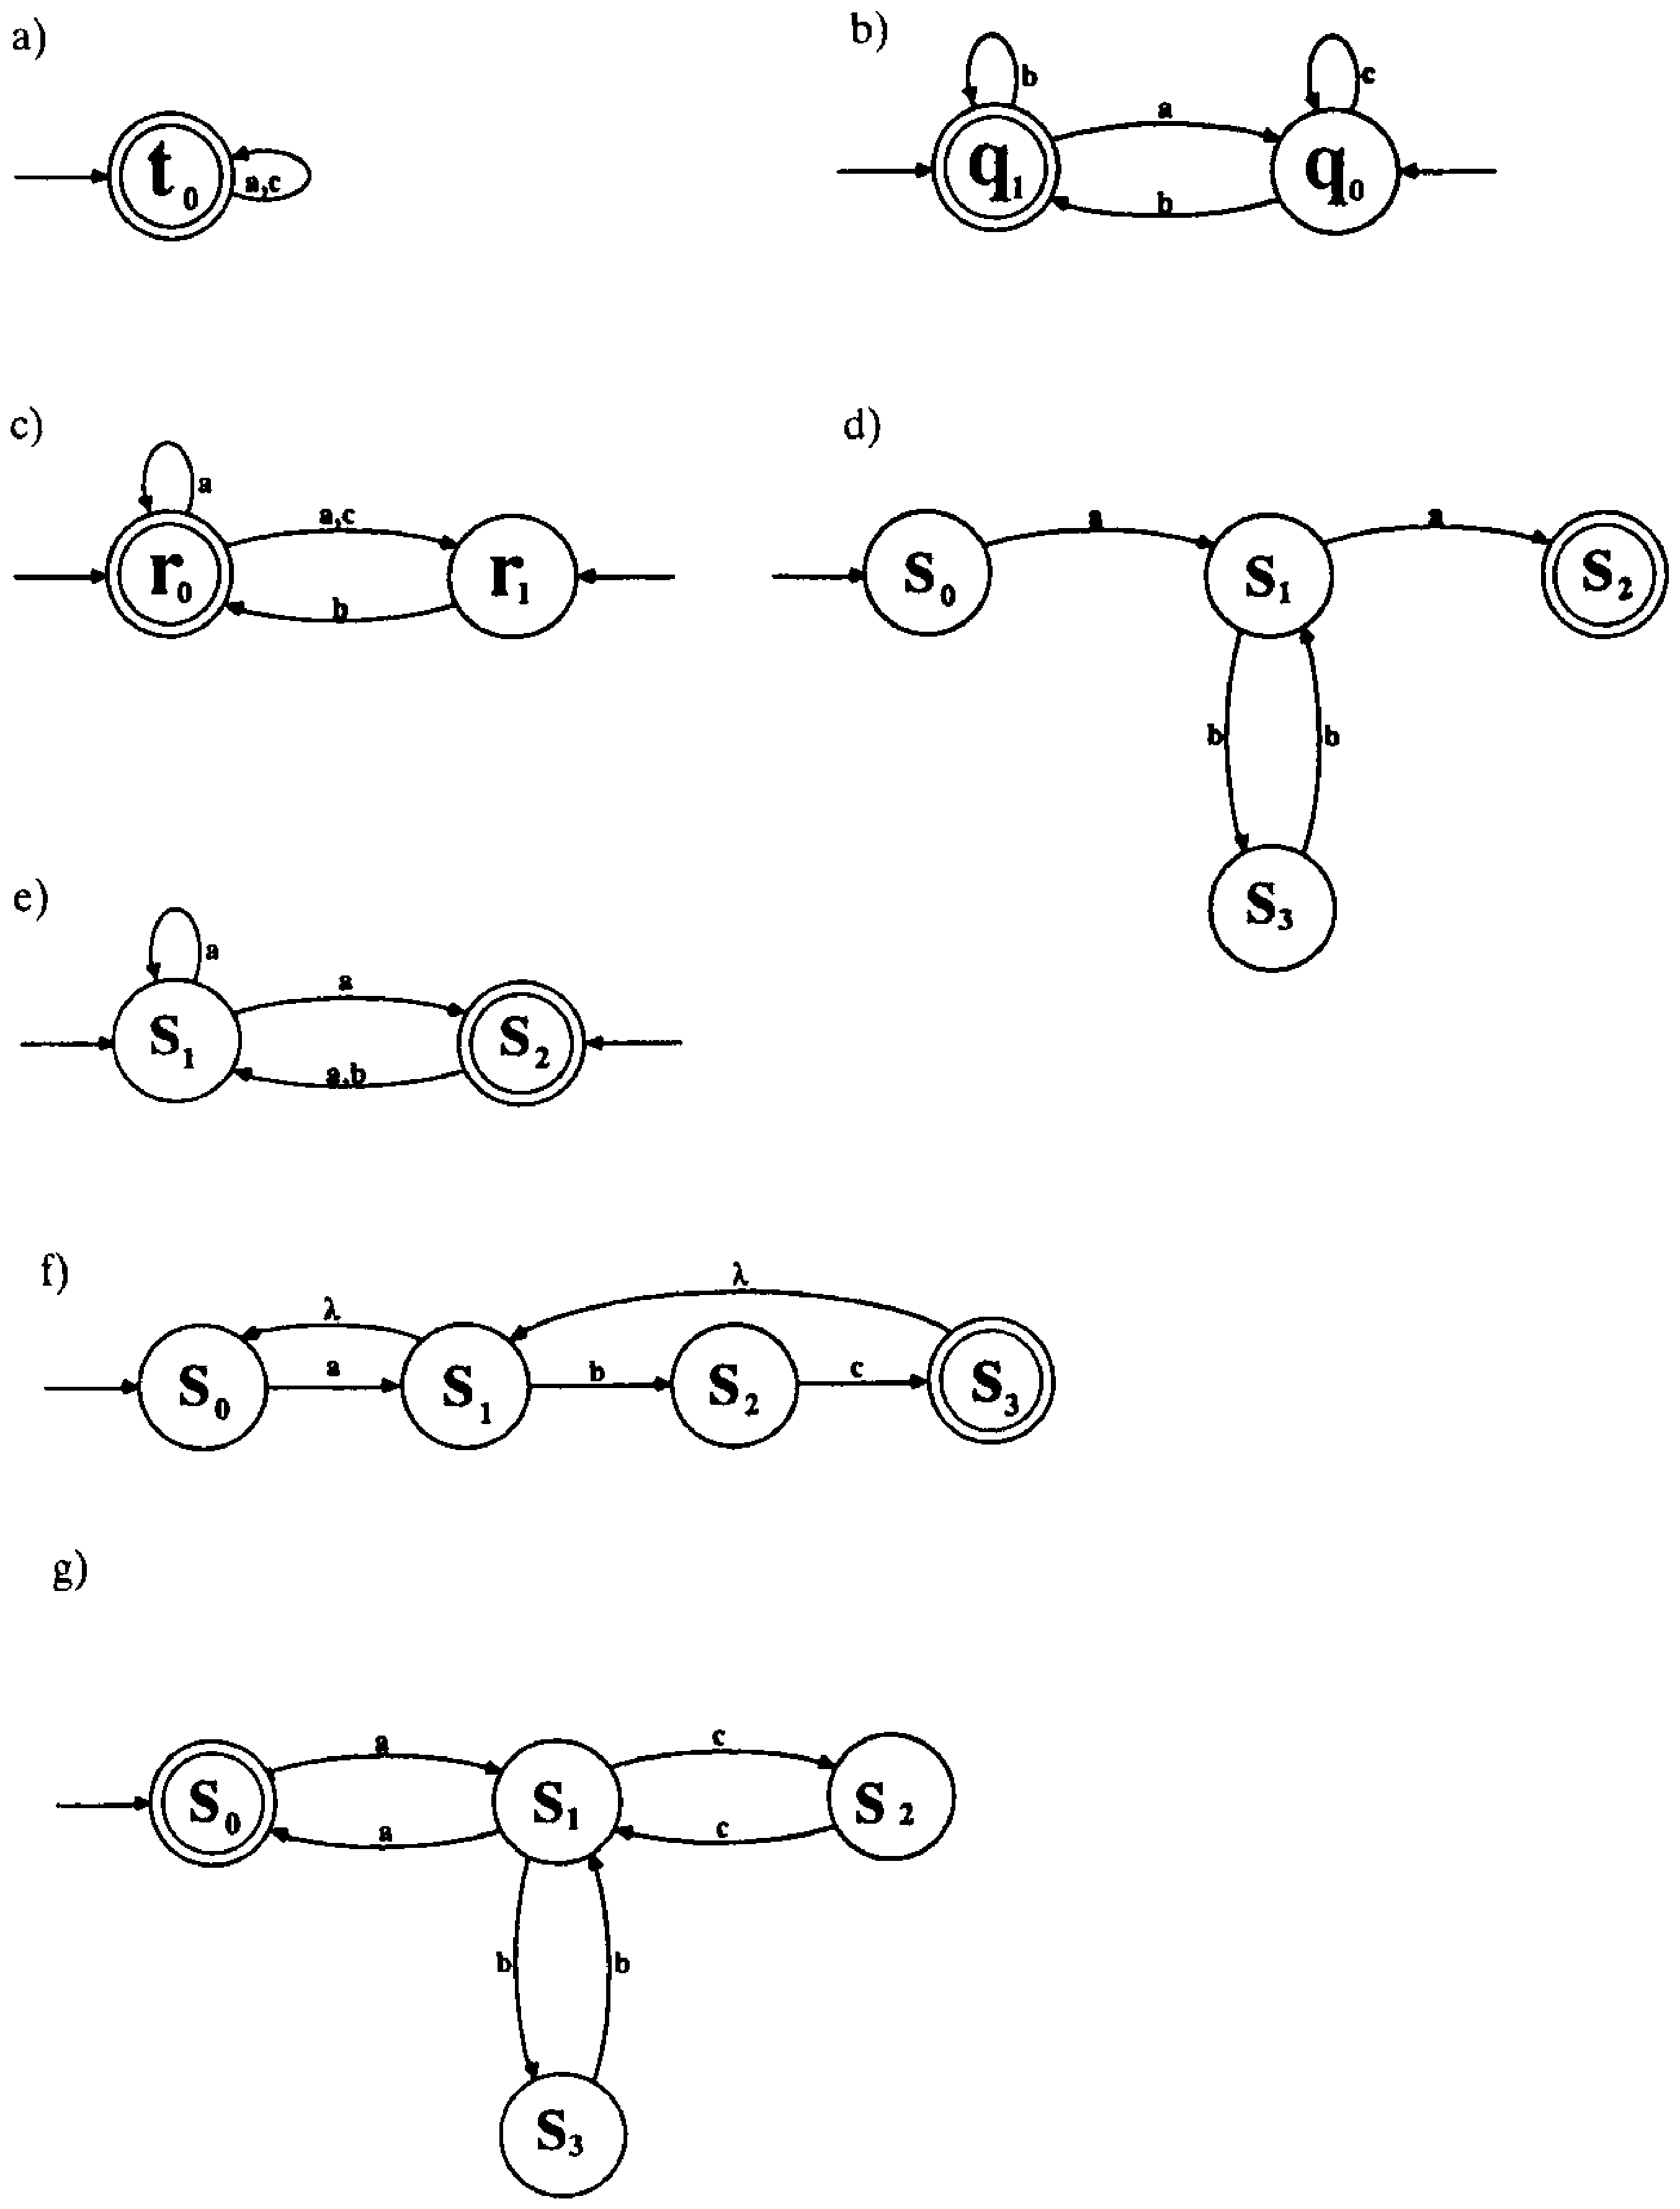
\epsfig{figure=ToFAfigures/fig6-14.eps,width=6.2in}}
\caption{The automata for Exercise 6.50}\label{fig-6.14}
\end{figure}

\item Let $\pmb{F}$ be the collection of languages that can be formed by repeated
application of the following five rules:
\begin{enumerate}[i.]
\item $\{\pmb{a}\}\in \pmb{F}$ and $\{\pmb{b}\}\in \pmb{F}$
\item $\{\ \}\in \pmb{F}$
\item $\{\lambda\}\in \pmb{F}$
\item If $F_1\in \pmb{F}$ and $F_2 \in \pmb{F}$, then $F_1 \cdot F_2 \in \pmb{F}$
\item If $F_1 \in \pmb{F}$ and $F_2 \in \pmb{F}$, then $F_1 \cup F_2 \in \pmb{F}$
\end{enumerate}
Describe the class of languages generated by these five rules.
\end{enumerate}

% Chapter, Section, Figure, Table, Theorem, Corollary, Lemma, Definition, {\bf       
\chapter{Finite-State Transducers}\label{ch-7}

We have seen that finite-state acceptors are by no means robust enough to accept
standard computer languages like Pascal. Furthermore, even if a DFA could
reliably recognize valid Pascal programs, a machine that only indicates ``Yes,
this is a valid program'' or ``No, this is not a valid program'' is certainly
not all we expect from a compiler. To emulate a compiler, it is necessary to
have a mechanism that will produce some \emph{output} other than a simple yes or
no: in this case, we would expect the corresponding machine language code (if
the program compiled successfully) or some hint as to the location and nature of
the syntax errors (if the program was invalid).

A machine that accepts input strings and \emph{translates} them into output
strings is called a \emph{sequential machine}\index{sequential machine|see{transducer}} or
\emph{\Index{transducer}}. Our conceptual picture of such a device is only
slightly different from the model of a DFA shown in Figure \ref{fig-7.1}a. We still have
a finite-state control and an input tape with a read head, but the accept/reject
indicator is replaced by an output tape and writing device, as shown in Figure
\ref{fig-7.1}b.

These machines do not have the power to model useful compilers, but they can
be employed in many other areas. Applications of sequential machine concepts
are by no means limited to the computer world or even to the normal connotations
associated with ``read'' and ``write.'' A vending machine is essentially a
transducer that interprets inserted coins and button presses as valid inputs and
returns candy bars and change as output. Elevators, traffic lights, and many
other common devices that monitor and react to limited stimuli can be modeled by
finite-state transducers.

The vending machine analogy illustrates that the types of input to a device
(coins) may be very different from the types of output (candy bars). In terms
of our conceptual model, the read head may be capable of recognizing symbols
that are different from those that the output head can print. Thus we will have
an \emph{output alphabet}\index{C@$\Gamma$|see {output alphabet}} $\Gamma$ that is not necessarily the same as
our \emph{input alphabet} $\Sigma$.

% Figure 7.1
\begin{figure}
\centerline{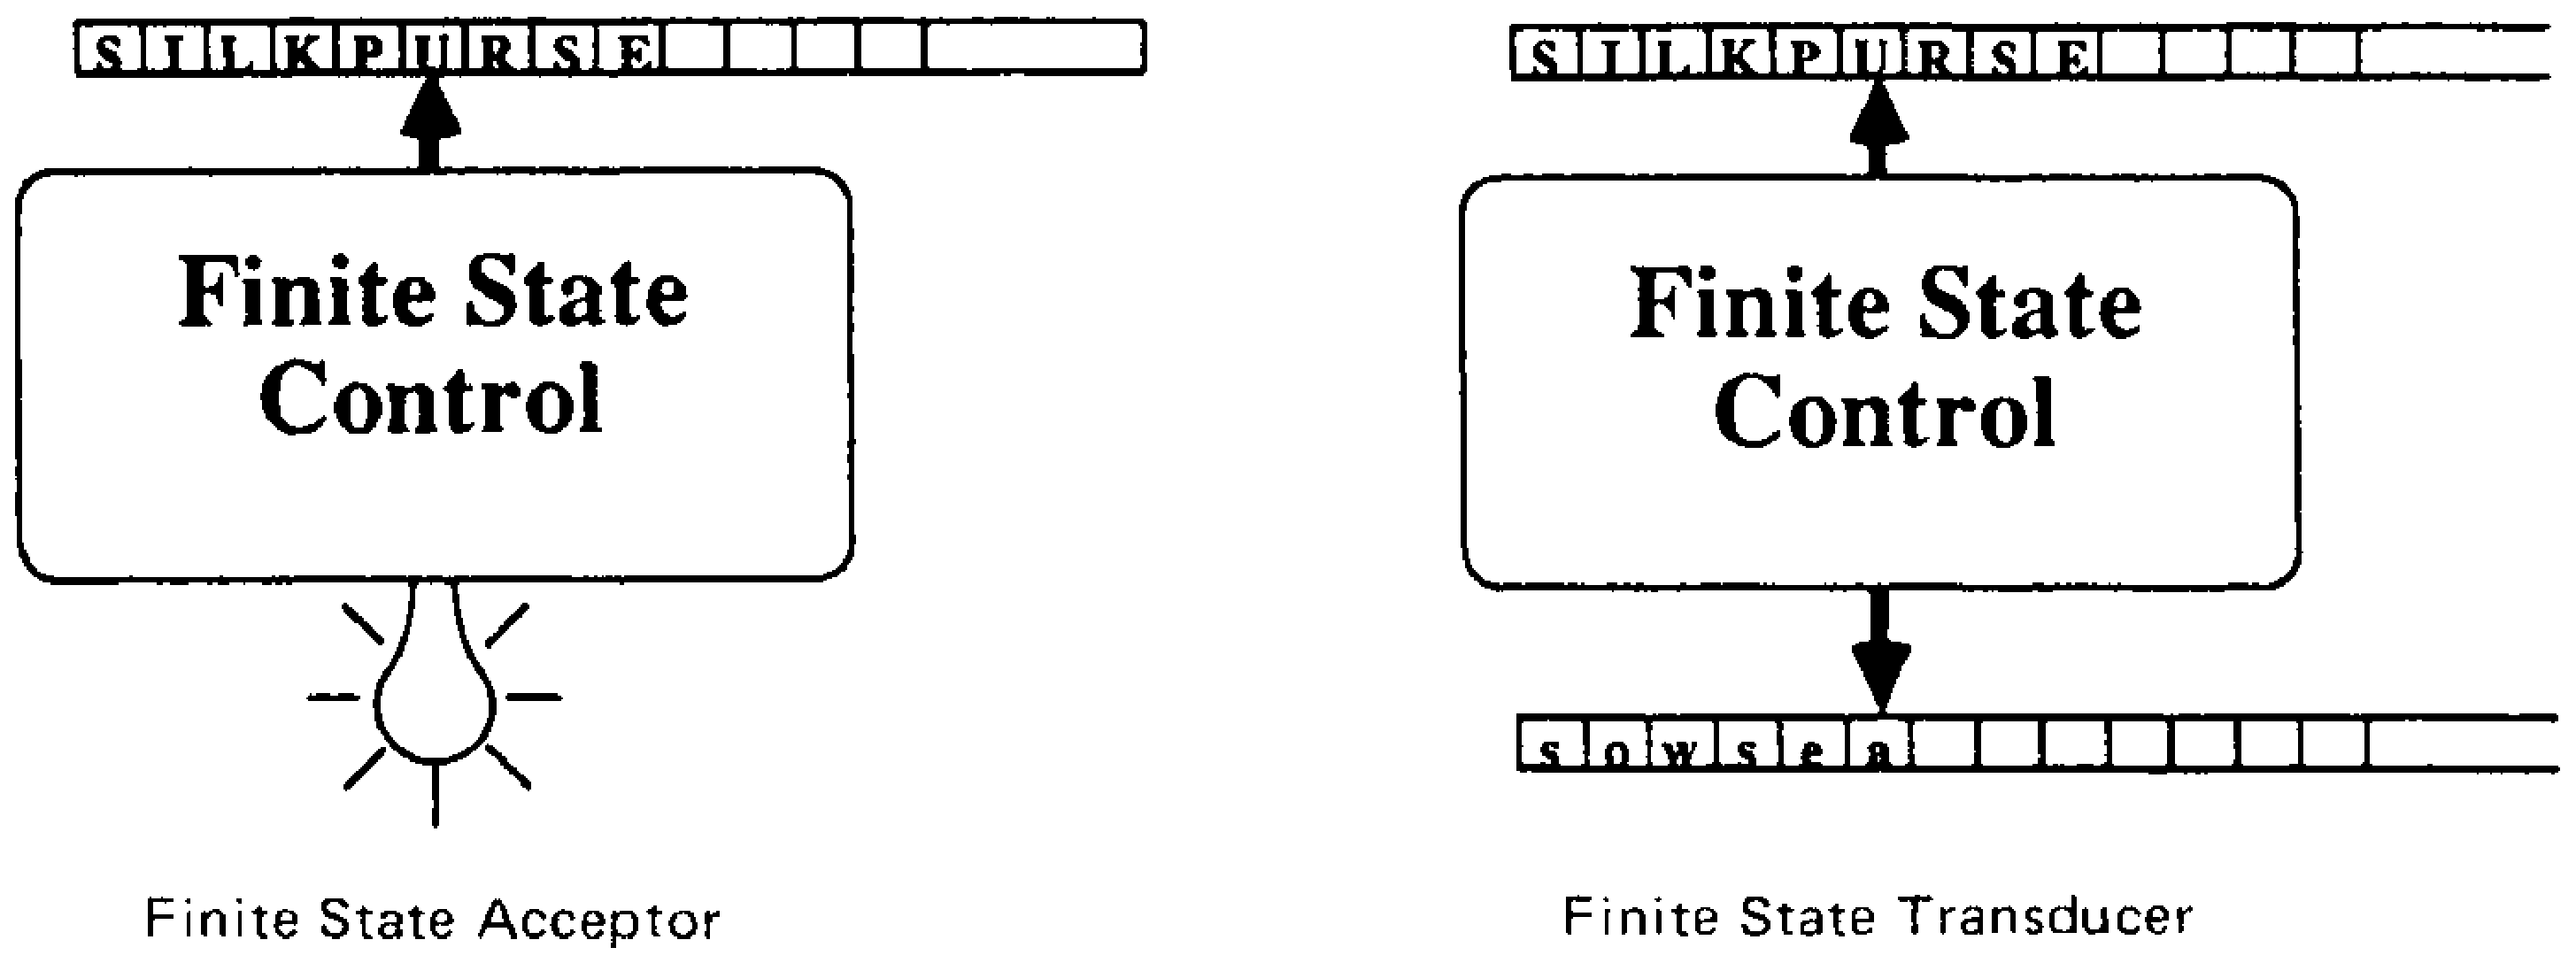
\epsfig{figure=ToFAfigures/fig7-1.eps,width=6in}}
\caption{The difference between an acceptor and a transducer}\label{fig-7.1}
\end{figure}

Also essential to our model is a rule that governs what characters are printed.
For our first type of transducer, this rule will depend on both the current
internal state of the machine and the current symbol being scanned by the read
head and will be represented by the function $\omega$. Finally, since we are
dealing with translation rather than acceptance/rejection, there is no need to
single out accepting states: the concept of final states can be dispensed with
entirely.

\section{Basic Definitions}\label{sec-7.1}

% Definition 7.1
\begin{dfn}\label{dfn-7.1}\index{alphabet!input}\index{alphabet!output}{\index{finite-state transducer|see{FST}}}\index{output alphabet}\index{state transition function!for FST}
A \emph{finite-state transducer} (\Index{FST}) or
\emph{Mealy sequential machine}\index{Mealy sequential machine|see{FST}}
with a distinguished start state is a sextuple
$\langle\Sigma,\Gamma,S,s_0,\delta,\omega\rangle$, where:
\begin{enumerate}[i.]
\item $\Sigma$ denotes the input alphabet.
\item $\Gamma$ denotes the output alphabet.
\item $S$ denotes the set of states, a finite nonempty set.
\item $s_0$ denotes the \emph{\Index{start state}}; $s_0 \in S$.
\item $\delta$ denotes the state transition function; $\delta$$: S \times \Sigma
	\rightarrow S$.
\item $\omega$ denotes the output function; $\omega$$: S \times \Sigma \rightarrow
	\Gamma$.
\end{enumerate}
\end{dfn}

The familiar state transition diagram needs to be slightly modified to represent
these new types of machines. Since there is one labeled arrow for each ordered
pair in the domain of the state transition function and there is also one output
symbol for each ordered pair, we will place the appropriate output symbol by its
corresponding arrow, and separate it from the associated input symbol by a
slash, /.

\subsection*{Example 7.1}

Let $V=\langle\{\pmb{n},\pmb{d},\pmb{q},\pmb{b}\},\{\pmb{\varphi},\pmb{n'},
\pmb{d'},\pmb{q'},\pmb{c}_0,\pmb{c}_1,\pmb{c}_2,\pmb{c}_3,\pmb{c}_4\},S,s_0,
\delta,\omega\rangle$ be the FST illustrated in Figure \ref{fig-7.2}. $V$ describes the
action of a candy machine that dispenses 30\cent\  Chocolate Explosions. $\pmb{n},
\ \pmb{d},\ \pmb{q}$ denote inputs of nickels, dimes, and quarters
(respectively), and $\pmb{b}$ denotes the act of pushing the button to select a
candy bar. $\pmb{\varphi},\pmb{n'},\pmb{d'},\pmb{q'},\pmb{c}_0,\pmb{c}_2,
\pmb{c}_2,\pmb{c}_3,\pmb{c}_4$ represent the vending machine's response to these
inputs: it may do nothing, return the nickel that was just inserted, return the
dime, return the quarter, or dispense a candy bar with 0, 1, 2, 3, or 4 nickels
as change, respectively. Note that the transitions agree with the vending
machine model presented in Chapter \ref{ch-1}; the new model now specifies the action
corresponding to the given input. It is relatively simple to modify the above
machine to include a new input $r$ that signifies that the coin return has been
activated and a new output a representing the release of all coins that have
been inserted (see the exercises).\index{vending machine!FST}

% Figure 7.2
\begin{figure}
\centerline{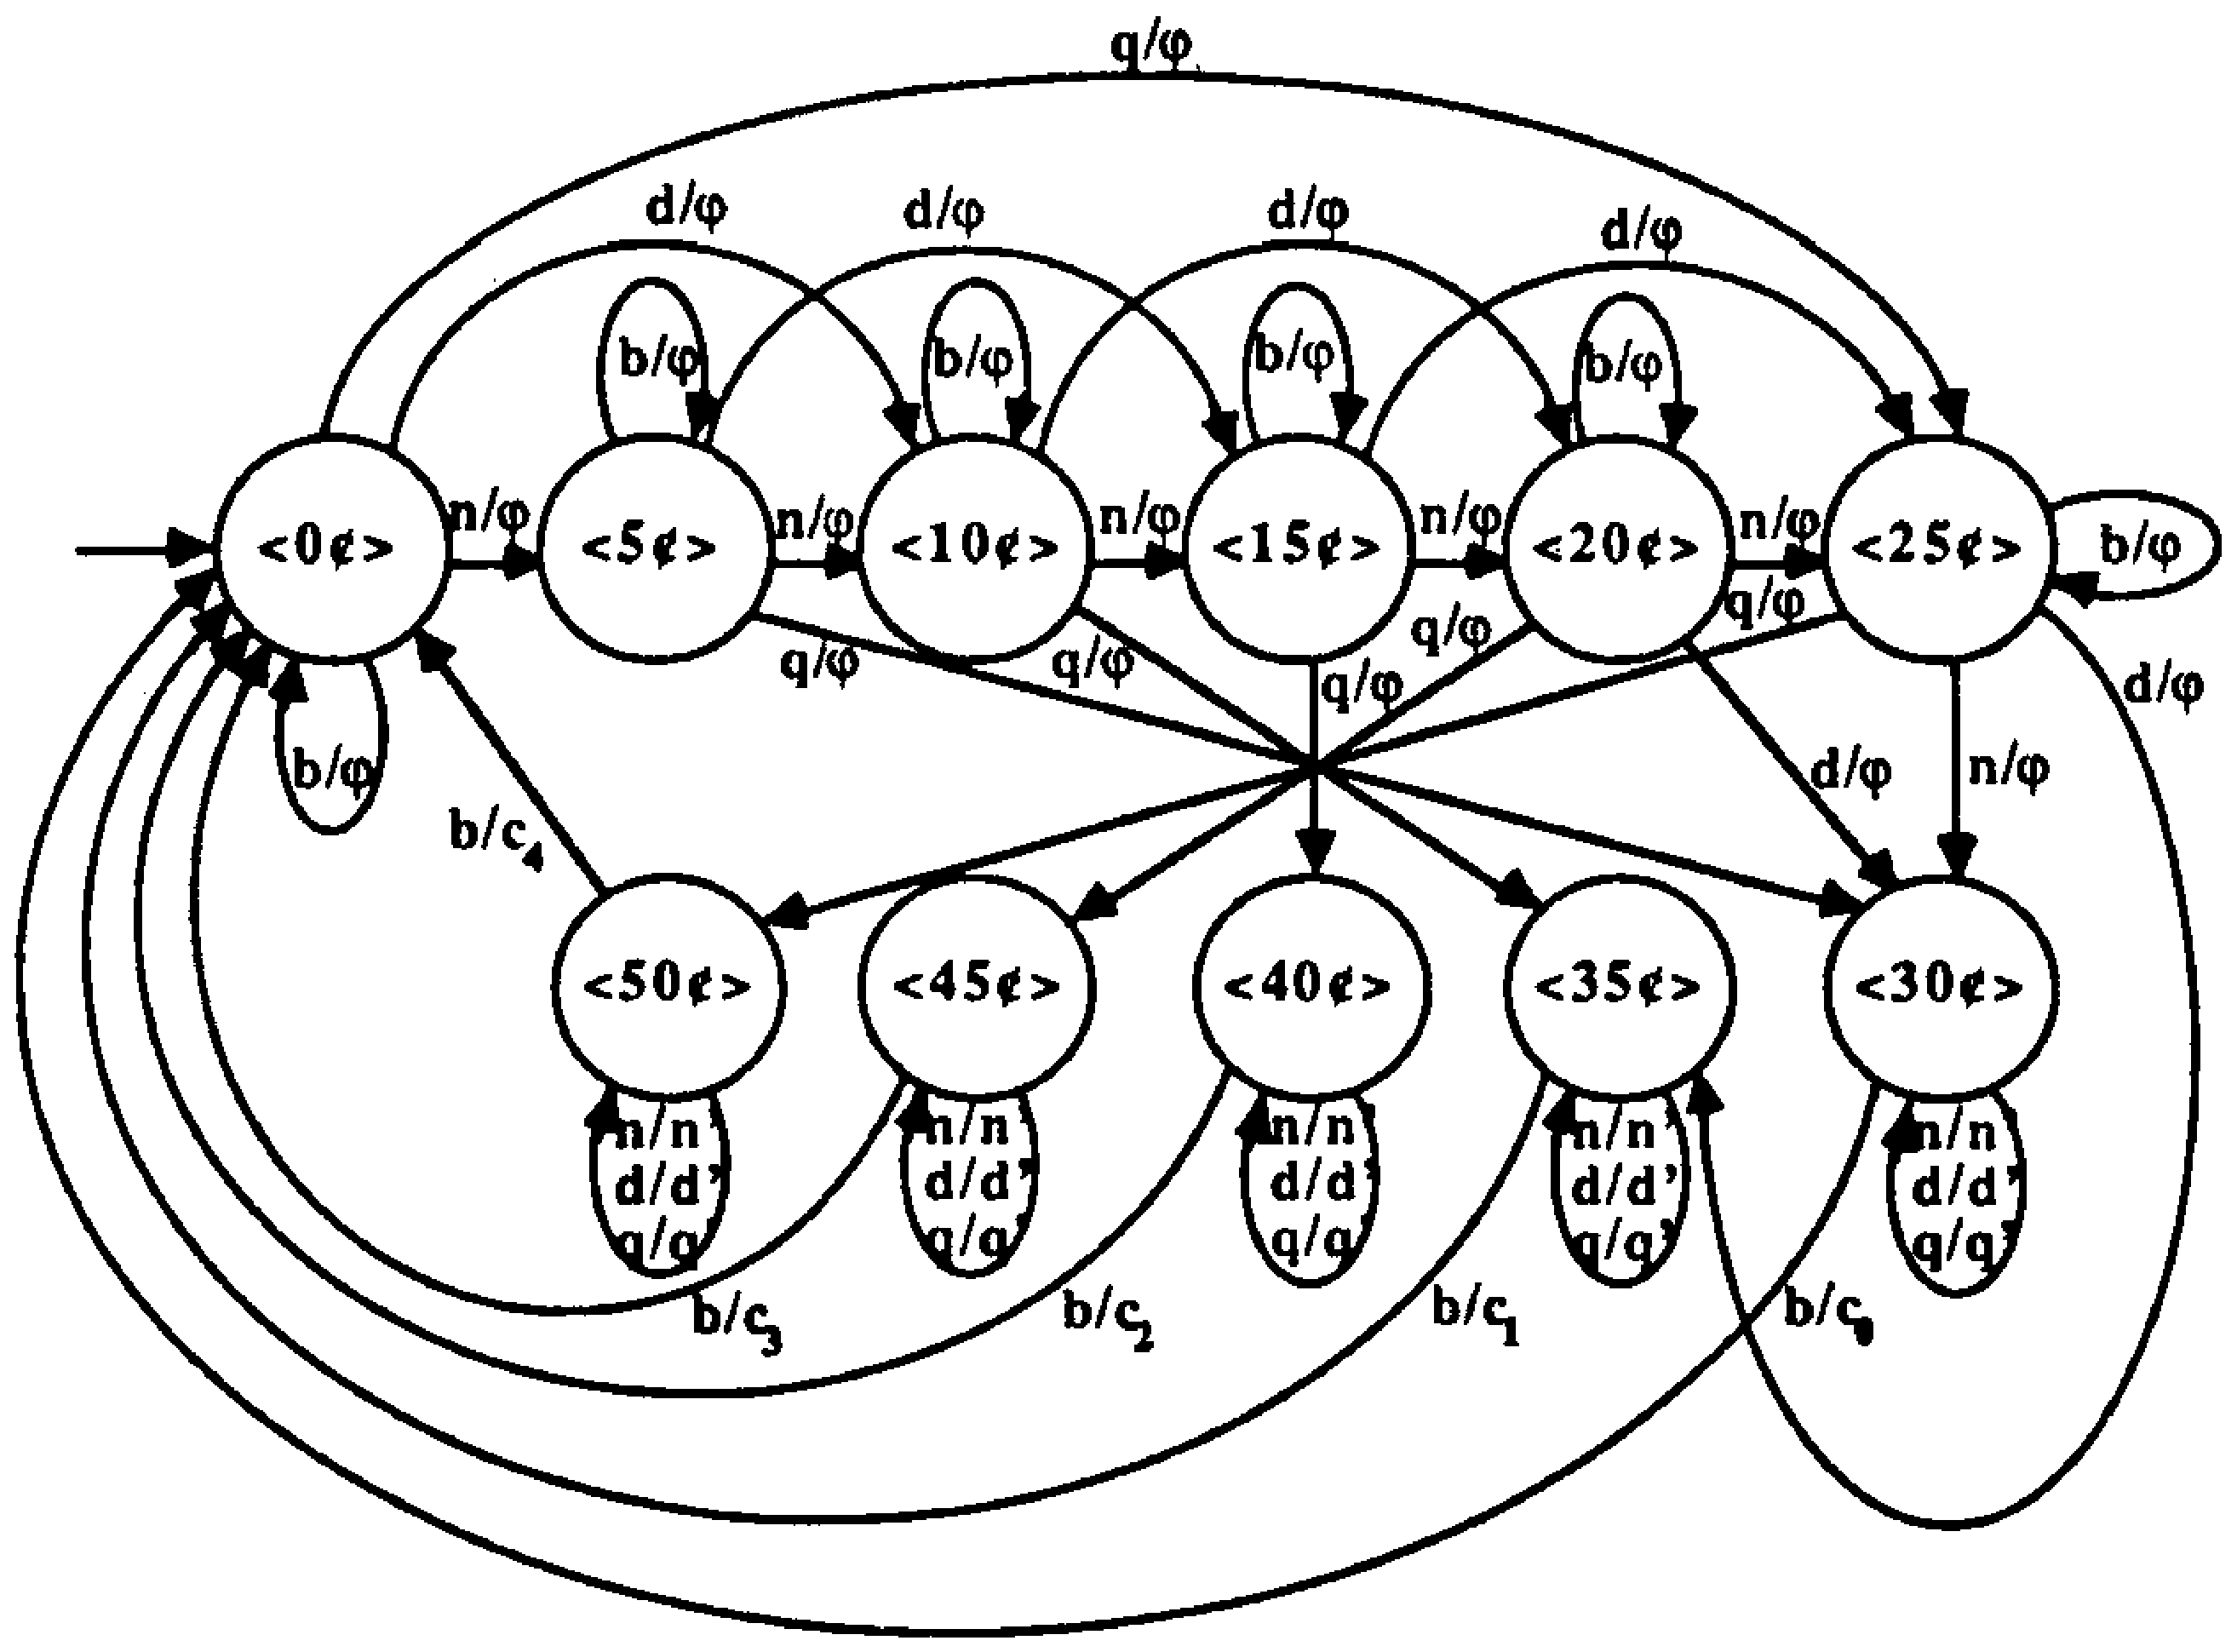
\epsfig{figure=ToFAfigures/fig7-2.eps,width=5.2in}}
\caption{A finite-state transducer model of the vending machine discussed in
Example 7.1}\label{fig-7.2}
\end{figure}

Various modern appliances can be modeled by FSTs. Many microwave ovens accept
input through the door latch mechanism and an array of keypad sensors, and
typical outputs include the control lines to the microwave generator, the
elements of a digital display, an interior light, and an audible buzzer. The
physical circuitry needed to implement these common machines will be discussed
in a later section. We now examine the ramifications of Definition \ref{dfn-7.1} by
concentrating on the details of a very simple finite-state transducer.

\subsection*{Example 7.2}

Let $B=\langle\Sigma,\Gamma,S,s_0,\delta,\omega\rangle$ be given by
\begin{center}
\begin{tabular}{l}
$\Sigma =\{\pmb{a},\pmb{b}\}$ \\
$\Gamma=\{\pmb{0},\pmb{1}\}$ \\
$S = \{s_0,s_1\}$ \\
$s_0 = s_0$
\end{tabular}
\end{center}
The state transition function is defined in Table 7.1a.

% Table 7.1a
% Tables are hand titled due to subnumbering.
\begin{table}[h]\label{tbl-7.1a}
\begin{center}
\begin{tabular}{c|cc}
\multicolumn{3}{c}{Table 7.1a} \\
$\delta$ & $\pmb{a}$ & $\pmb{b}$ \\
\hline
$s_0$ & $s_0$ & $s_1$ \\
$s_1$ & $s_0$ & $s_1$ \\
\end{tabular}
\end{center}
\end{table}
It can be more succinctly specified by ($\forall s \in S)[\delta(s,\pmb{a}) =
s_0$ and $\delta(s,\pmb{b}) = s_1]$. Finally, Table 7.1b displays the
output function, which can be summarized by
$ (\forall c \in \Sigma)[\omega(s_0,c)=0\quad\text{and}\quad\omega(s_1,c) =
	\pmb{1}] $
% Table 7.1b
\begin{table}[h]\label{tbl-7.1b}
\begin{center}\begin{tabular}{c|cc}
\multicolumn{3}{c}{Table 7.1b} \\
$\omega$ & $\pmb{a}$ & $\pmb{b}$ \\
\hline
$s_0$ & $\pmb{0}$ & $\pmb{0}$ \\
$s_1$ & $\pmb{1}$ & $\pmb{1}$
\end{tabular}\end{center}
\end{table}

All the information about $B$ is contained in the diagram displayed in Figure
\ref{fig-7.3}. Consider the input sequence $z=\pmb{abaabbaa}$. From $s_0$, the first
letter of $z$, that is, $\pmb{a}$, causes a $\pmb{0}$ to be printed, since
$\omega(s_0,\pmb{a}) = \pmb{0}$, and since $\delta(s_0,\pmb{a}) = s_0$, the
machine remains in state $s_0$. The second letter $\pmb{b}$ causes a second
$\pmb{0}$ to be printed since $\omega(s_0,\pmb{b}) =\pmb{0}$, but the machine
now switches to state $s_1\ [\delta(s_0,\pmb{b}) = s_1]$. The third input letter
causes a $\pmb{1}$ to be printed $[\omega(s_1,\pmb{a})=\pmb{1}]$, and so on. The
entire output string will be $\pmb{00100110}$, and the machine, after starting
in state $s_0$, will successively assume the state $s_0,s_1,s_0,s_0,s_1,s_1,s_0,
s_0$ as the input string is processed. We are not currently interested in the
terminating state for a given string ($s_0$ in this case), but rather in the
resulting output string, $\pmb{00100110}$.

% Figure 7.3
\begin{figure}
\centerline{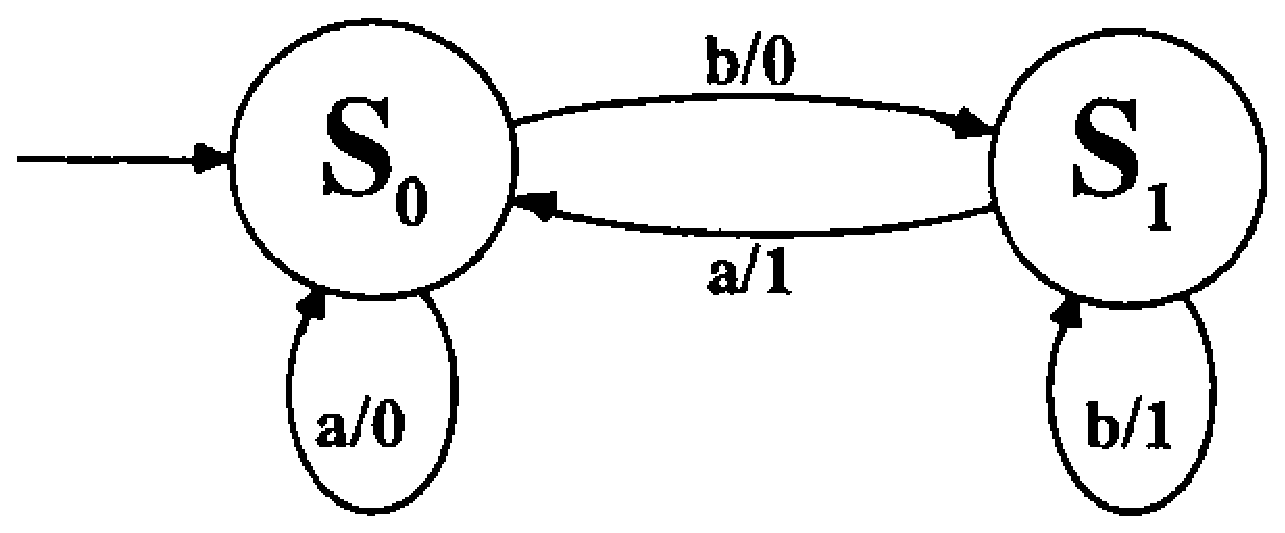
\epsfig{figure=ToFAfigures/fig7-3.eps,width=2in}}
\caption{The state transition diagram for the transducer discussed in Example
7.2}\label{fig-7.3}
\end{figure}

It should be clear that the above discussion illustrates a very awkward way of
describing translations. While $\omega$ describes the way in which single
\emph{letters} are translated, the study of finite-state transducers will
involve descriptions of how entire \emph{strings} are translated. This situation
is reminiscent of the modification of the state transition function $\delta$,
which likewise operated on single letters, to the extended state transition
function $\DBAR$ (which was defined for \emph{strings}). Indeed, what is called
for is an extension of $\omega$ to \OBAR, which will encompass the translation
of entire strings. The translation cited in the last example could then be
succinctly stated as $\OBAR(s_0,\pmb{abaabbaa})=\pmb{00100110}$. That is, the
notation $\OBAR(t,y)$ is intended to represent the output string produced by a
transducer (beginning from state $t$) in response to the input string $y$.

The formal recursive definition of \OBAR\ will depend not only on $\omega$ but
also on the state transition function $\delta$ (and its extension \DBAR).
$\delta$ retains the same conceptual meaning it had for finite-state acceptors:
$\DBAR(s,x)$ denotes the state reached when starting from $s$ and processing, in
sequence, the individual letters of the string $x$. Furthermore, the conclusion
stated in Theorem \ref{thm-1.1} still holds:
\[ (\forall x \in \Sigma^*)(\forall y \in \Sigma^*)(\forall s \in S)(\DBAR(s,yx)
	=\DBAR(\DBAR(s,y),x)) \]
A similar statement can be made about $\omega$ once it has been rigorously
defined.

% Definition 7.2
\begin{dfn}\label{dfn-7.2}\index{extended state transition function \DBAR\! for FST}\index{extended output function \OBAR\! for FST}
Given a FST $A=\langle\Sigma,\Gamma,S,s_0,\delta,\omega\rangle$, the extended
output function for $A$, denoted by \OBAR, is a function $\OBAR$$: S \times
\Sigma^* \rightarrow \Gamma^*$ defined recursively as follows:
\begin{enumerate}[i. ]
% handspaced vs. hardcoding i., ii.
\item $(\forall t \in S)\qquad\qquad\qquad\qquad\ \ \ \thinspace\thinspace\OBAR
	(t,\lambda)=\lambda$
\item $(\forall t \in S)(\forall x \in \Sigma^*)(\forall a \in \Sigma)
	(\OBAR(t,\pmb{a}x)=\omega(t,\pmb{a})\cdot\OBAR(\delta(t,\pmb{a}),x))$
\end{enumerate}
\end{dfn}

\subsection*{Example 7.3}

Let $B=\langle\Sigma,\Gamma,S,s_0,\delta,\omega\rangle$ be the FST given in
Example 7.2. Then
\begin{center}
\begin{tabular}{rl}
$\OBAR(s_1,\pmb{baa})$ & $=\omega(s_1,\pmb{b}) \cdot \OBAR(\delta(s_1,\pmb{b}),
	\pmb{aa}) = \pmb{1} \cdot \OBAR(s_1,\pmb{aa})$ \\
& $= \pmb{1} \cdot \omega(s_1,\pmb{a})\cdot\OBAR(\delta(s_1,\pmb{a}),\pmb{a}) =
	\pmb{11}\cdot \OBAR(s_0,\pmb{a}) = \pmb{110}$
\end{tabular}
\end{center}
Note that a three-letter input sequence gives rise to exactly three output
symbols: $\OBAR$ is \emph{\Index{length preserving}}, in the sense that
$(\forall t \in S)(\forall x \in \Sigma^*)(|\OBAR(t,x)| = |x|)$.

The \OBAR\ function extends the $\omega$ function from single letters to words.
Whereas the $\omega$ function maps a state and a \emph{letter} to a single
symbol from $\Gamma$, the \OBAR\ function maps a state and a \emph{word} to an
entire \emph{string} from $\Gamma^*$. It can be deduced from (i) and (ii) (see
the exercises) that (iii) ($\forall t \in S)(\forall a \in \Sigma)(\OBAR(t, a)
= \omega(t,a))$, which is the observation that $\omega$ and \OBAR\ treat single
letters the same. The extended output function \OBAR\ has properties similar to
those of \DBAR, in that the single letter $\pmb{a}$ found in the recursive
definition of \OBAR\ can be replaced by an entire word $y$. The analog of
Theorem \ref{thm-1.1} is given below.

% Theorem 7.1
\begin{thm}\label{thm-7.1}
Let $A=\langle\Sigma,\Gamma,S,s_0,\delta,\omega\rangle$ be a FST. Then:
\[ (\forall x \in \Sigma^*)(\forall y \in \Sigma^*)(\forall t \in S)(\OBAR(t,yx)
	= \OBAR(t,y) \cdot \OBAR(\DBAR(t,y),x)) \]
and
\[ (\forall x \in \Sigma^*)(\forall y \in \Sigma^*)(\forall s \in S)(\DBAR(s,yx)
	= \DBAR(\DBAR(s,y),x)) \]

\emph{Proof.} The proof is by induction on $|y|$ (see the exercises and compare
with Theorem \ref{thm-1.1}).
\end{thm}

\subsection*{Example 7.4}

Let $B=\langle\Sigma,\Gamma,S,s_0,\delta,\omega\rangle$ be the FST given in
Example 7.2. Consider the string $z=\pmb{abaabbaa}=yx$, where $y=\pmb{abaab}$
and $x=\pmb{baa}$. To apply Theorem \ref{thm-7.1} with $t=s_0$, we first calculate
$\OBAR(s_0,y) = \OBAR(s_0,\pmb{abaab}) = \pmb{00100}$, and $\DBAR(s_0,y) = s_1$.
From Example 7.3, $\OBAR(s_1,\pmb{baa}) = \pmb{110}$, and hence, as required by
Theorem \ref{thm-7.1},
\[ \pmb{00100110} = \OBAR(s_0,\pmb{abaabbaa}) = \OBAR(s_0,yx) = \OBAR(s_0,y)
	\cdot \OBAR(\DBAR(s_0,y),x) = \pmb{00100} \cdot \pmb{110} \]

For a given FST $A$ with a specified start state, the deterministic nature of
finite-state transducers requires that each input string be translated into a
\emph{unique} output string; that is, the relation $f_A$ that associates input
strings with their corresponding output strings is a \emph{function}.

% Definition 7.3
\begin{dfn}\label{dfn-7.3}{\index{translation function!FST}}
Given a FST $M=\langle\Sigma,\Gamma,S,s_0,\delta,\omega\rangle$, the
\emph{translation function} for $M$, denoted by $f_M$, is the function
$f_M$$: \Sigma^* \rightarrow \Gamma^*$ defined by $f_M(x) = \OBAR(s_0,x)$.
\end{dfn}

Note that $f_M$, like \OBAR, is \emph{length preserving}:
$(\forall x \in \Sigma^*)(|f_M(x)| = |x|)$. Consequently, for any $n \in \NN$,
if the domain of $f_M$ were restricted to $\Sigma^n$, then the range of $f_M$
would likewise be contained in $\Gamma^n$.

\subsection*{Example 7.5}

Let $B=\langle\Sigma,\Gamma,S,s_0,\delta,\omega\rangle$ be the finite-state
transducer given in Figure \ref{fig-7.3}. Since $\OBAR(s_0,\pmb{abaab})=(\pmb{00100})$,
$f_B(\pmb{abaab}) = \pmb{00100}$. Similarly, $f_B(\lambda) = \lambda$,
$f_B(\pmb{a})=\pmb{0}$, $f_B(\pmb{b})=\pmb{0}$, $f_B(\pmb{aa})=\pmb{00}$,
$f_B(\pmb{ab})=\pmb{00}$, $f_B(\pmb{ba})=\pmb{01}$, $f_B(\pmb{bb})=\pmb{01}$.
Coupled with these seven base definitions, this particular $f_B$ could be
recursively defined by
\begin{align*}
(\forall x \in \Sigma^*)f_B(x\pmb{aa}) = f_B(x\pmb{a}) \cdot \pmb{0} \\
f_B(x\pmb{ab}) = f_B(x\pmb{a}) \cdot \pmb{0} \\
f_B(x\pmb{ba}) = f_B(x\pmb{b}) \cdot \pmb{1}
\intertext{and}f_B(x\pmb{bb}) = f_B(x\pmb{b}) \cdot \pmb{1}
\end{align*}
$f_B$ in essence replaces $\pmb{a}$s with $\pmb{0}$s and $\pmb{b}$s with $\pmb{1}$s,
and ``delays'' the output by one letter. More specifically, the translation
function for $B$ takes an entire string and substitutes $\pmb{0}$s and
$\pmb{1}$s for $\pmb{a}$s and $\pmb{b}$s (respectively), deletes the last letter of
the string, and appends a $\pmb{0}$ to the front of the resulting string. The
purpose of the two states $s_0$ and $s_1$ in the FST $B$ is to remember whether
the previous symbol was an $\pmb{a}$ or a $\pmb{b}$ (respectively) and output the
appropriate replacement letter. Note that $\pmb{1}$s are always printed on
transitions from $s_1$, and $\pmb{0}$s are printed as we leave $s_0$.

\subsection*{Example 7.6}

Let $C=\langle\{\pmb{a},\pmb{b}\},\{\pmb{0},\pmb{1}\},\{t_0,t_1,t_2,t_3\},t_0,
\delta_C,\omega_C\rangle$ be the FST shown in Figure \ref{fig-7.4}. $C$ \emph{flags}
occurrences of the string $\pmb{aab}$ by printing a $\pmb{1}$ on the output tape
\index{tape!output} only when the substring $\pmb{aab}$ appears in the input stream.

% Figure 7.4
\begin{figure}
\centerline{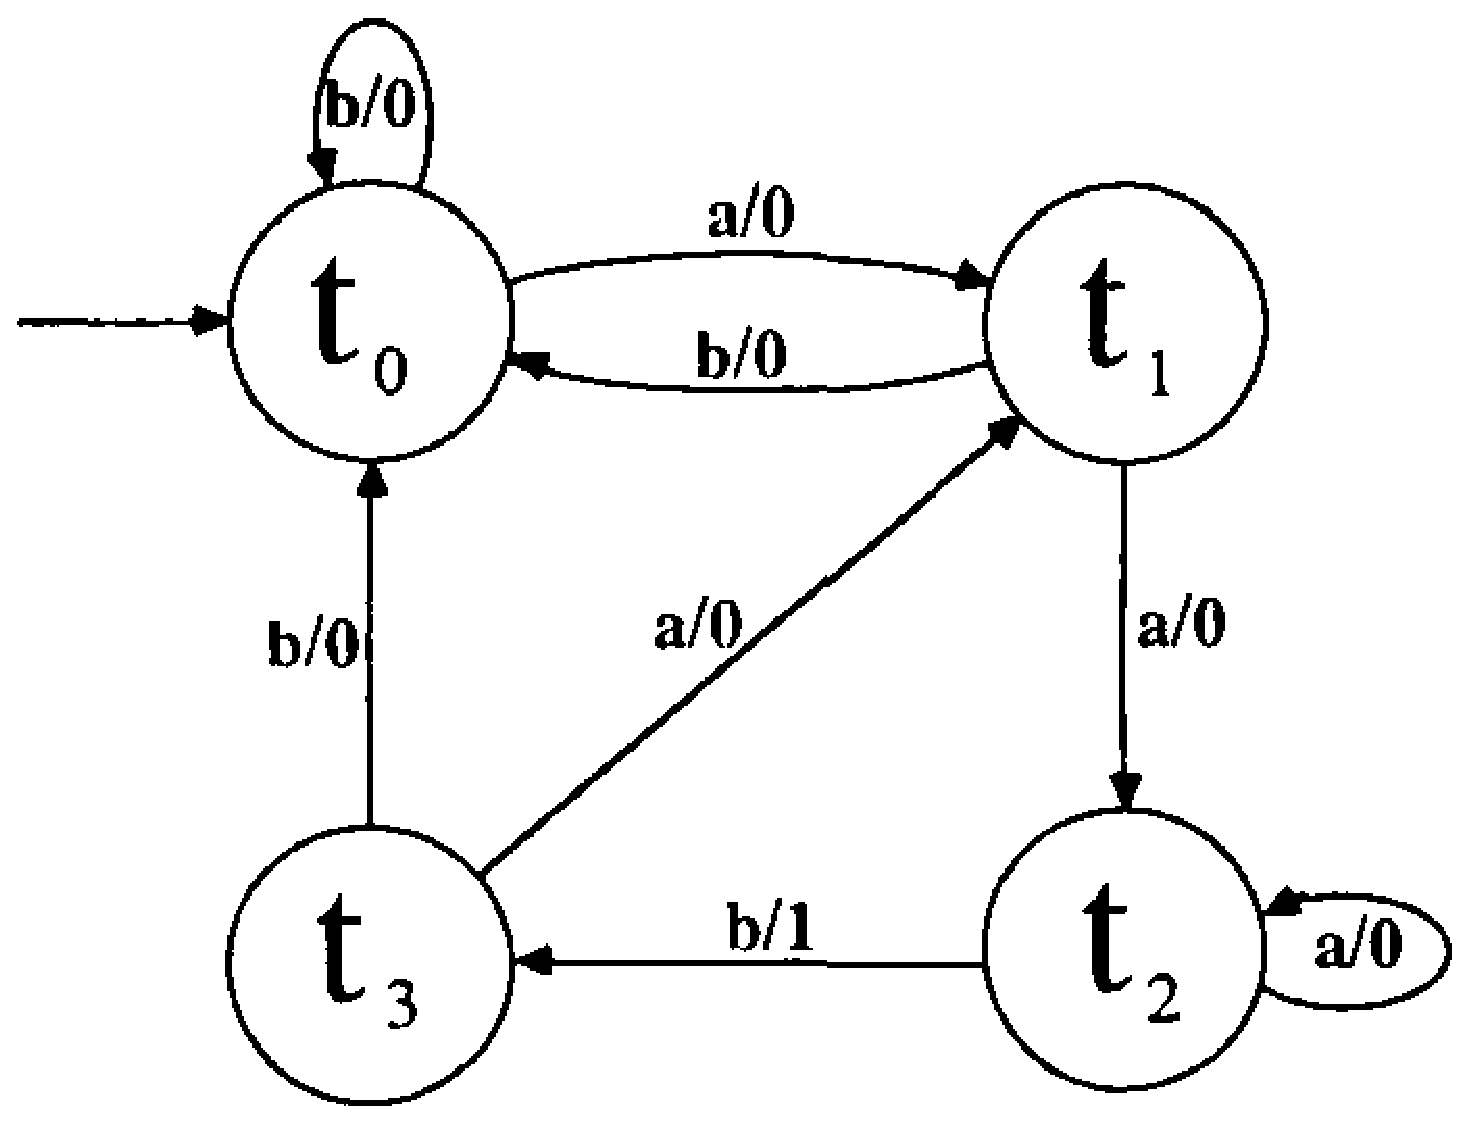
\epsfig{figure=ToFAfigures/fig7-4.eps,width=2.5in}}
\caption{The state transition diagram for the Mealy machine $C$ in
Example 7.6}\label{fig-7.4}
\end{figure}

Clearly, not all functions from $\Sigma^*$ to $\Gamma^*$ can be represented by
finite-state transducers; we have already observed that functions that are not
length preserving cannot possibly qualify. As the function discussed later in
Example 7.7 shows, not all length-preserving functions qualify, either.

% Definition 7.4
\begin{dfn}\label{dfn-7.4}
Given a function $f$$: \Sigma^* \rightarrow \Gamma^*,\ f$ is \emph{finite transducer definable}\index{finite
transducer definable|see{FTD}} (\Index{FTD}) iff there exists a transducer $A$ such
that $f=f_A$.
\end{dfn}

Due to the deterministic nature of transducers, any two strings that ``begin
the same'' must start being ``translated the same.'' This observation is the
basis for the following theorem.

% Theorem 7.2
\begin{thm}\label{thm-7.2}
Assume $f$ is FTD. Then

%\begin{tabular}{l}
$(\forall n \in \NN)(\forall x \in \Sigma^n)(\forall y \in \Sigma^*)
	(\forall z \in \Sigma^*)(\text{the first }n\text{ letters of }f(xy)$ 
	must agree with the first $n$ letters of $f(xz))$
%\end{tabular}

\emph{Proof.} See the exercises.
\end{thm}

\subsection*{Example 7.7}

Consider the function $g$$:\{\pmb{a},\pmb{b},\pmb{c}\}^* \rightarrow
\{\pmb{0},\pmb{1}\}^*$, which replaces input symbols by $\pmb{0}$ unless the
next letter is $\pmb{c}$, in which case $\pmb{1}$ is used instead. Thus,
\[ g(\pmb{abcaaccb}) = \pmb{01001100}\text{ and }g(\pmb{abb}) = \pmb{000}. \]
With $n = 2$, choosing $x = \pmb{ab}$, $y = \pmb{caaccb}$, and $z = \pmb{b}$
shows that $g$ violates Theorem \ref{thm-7.2}, so $g$ cannot be FTD.

The necessary condition outlined in the previous theorem is by no means
sufficient to guarantee that a function is FTD; other properties such as a
pumping lemma-style repetitiousness of the translation must also be present (see
the exercises).

\section{Minimization of Finite-State Transducers}\label{sec-7.2}

Two transducers that perform exactly the same translation over the entire range
of input strings from $\Sigma$ will be called \emph{equivalent} transducers.
This is in spirit similar to the way equivalence was defined for deterministic
finite automata.

% Definition 7.5
\begin{dfn}\label{dfn-7.5}\index{equivalent!transducers}
Given transducers
\[ A=\langle\Sigma,\Gamma,S_A,s_{0_A},\delta_A,\omega_A\rangle\quad\text{and}
	\quad B=\langle\Sigma,\Gamma,S_B,s_{0_B},\delta_B,\omega_B\rangle, \]
$A$ is said to be \emph{equivalent} to $B$ iff $f_A = f_B$.
\end{dfn}

Just as with finite automata, a reasonable goal when constructing a transducer
is to produce an efficient machine, and, as before, this will be equated with
the size of the finite-state control; given a translation function $f$, a
minimal machine for $f$ is a FST that has the minimum number of states necessary
to perform the required translation.

% Definition 7.6
\begin{dfn}\label{dfn-7.6}
Given a finite-state transducer
$A=\langle\Sigma,\Gamma,S_A,s_{0_A},\delta_A,\omega_A\rangle$, $A$ is the
\emph{\Index{minimal Mealy machine} for the translation} $f_A$ iff for all
finite-state transducers
$B=\langle\Sigma,\Gamma,S_B,s_{0_B},\delta_B,\omega_B\rangle$ for which
$f_A = f_B,\ \|S_A\| \leq \|S_B\|$.
\end{dfn}

Thus, $A$ is minimal if there is no equivalent machine with fewer states.

\subsection*{Example 7.8}

The FST $C=\langle\{\pmb{a},\pmb{b}\},\{\pmb{0},\pmb{1}\},\{t_0,t_1,t_2,t_3\},
t_0,\delta_C,\omega_C\rangle$ given in Figure \ref{fig-7.4} is \emph{not} minimal. The FST
$D=$\linebreak$\langle\{\pmb{a},\pmb{b}\},\{\pmb{0},\pmb{1}\},\{q_0,q_1,q_2\},q_0,\delta_D,
\omega_D\rangle$ given in Figure \ref{fig-7.5} performs the same translation, but has only
three states.\index{equivalent!transducers}

% Figure 7.5
\begin{figure}
\centerline{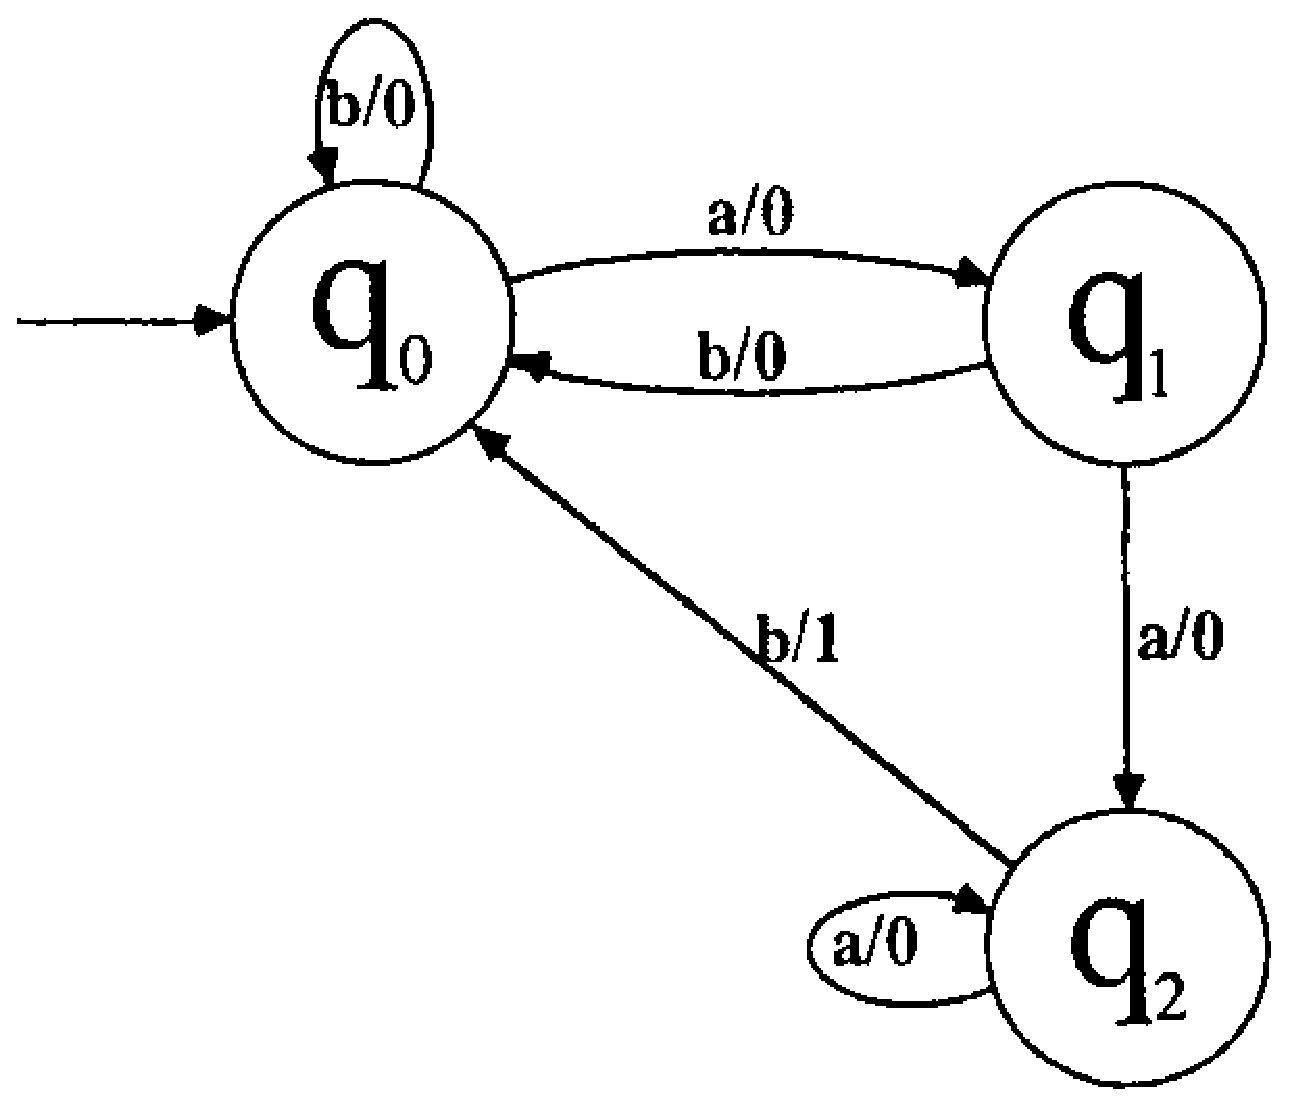
\epsfig{figure=ToFAfigures/fig7-5.eps,width=2.5in}}
\caption{The state transition diagram for the Mealy machine $D$ in Example 7.8}\label{fig-7.5}
\end{figure}

The concept of two transducers being essentially the same except for a trivial
renaming of the states will again be formalized through the definition of
\emph{isomorphism}\index{isomorphism!between FSTs} (and
\emph{homomorphism}).\index{homomorphism!between FSTs} As before, it will
be important to match the respective start states and state transitions; but
rather than matching up final states (which do not exist in the FST model), we
must instead ensure that the output function is preserved by the relabeling
process.

% Definition 7.7
\begin{dfn}\label{dfn-7.7}
Given two FSTs
\[ A=\langle\Sigma,\Gamma,S_A,s_{0_A},\delta_A,\omega_A\rangle\quad\text{and}
	\quad B=\langle\Sigma,\Gamma,S_B,s_{0_B},\delta_B,\omega_B\rangle, \]
and a function $\mu$$: S_A \rightarrow S_B,\ \mu$ is called a \emph{\Index{Mealy
machine homomorphism}} from $A$ to $B$ iff the following three conditions hold:
\begin{enumerate}[i.]
\item $\mu(s_{0_A}) = s_{0_B}$.
\item $(\forall s \in S_A)(\forall\pmb{a} \in \Sigma)(\mu(\delta_A(s,\pmb{a}))
	= \delta_B(\mu(s),\pmb{a}))$.
\item $(\forall s \in S_A)(\forall\pmb{a} \in \Sigma)(\omega_A(s,\pmb{a}) =
	\omega_B(\mu(s),\pmb{a}))$.
\end{enumerate}
\end{dfn}

As in Chapter \ref{ch-3}, a bijective homomorphism will be called an isomorphism and will
signify that the isomorphic machines are essentially the same (except perhaps
for the names of the states). The isomorphism is essentially a recipe for
renaming the states of one machine to produce identical transducers.

% Definition 7.8
\begin{dfn}\label{dfn-7.8}
Given two FSTs
\[ A=\langle\Sigma,\Gamma,S_A,s_{0_A},\delta_A,\omega_A\rangle\quad\text{and}
	\quad B=\langle\Sigma,\Gamma,S_B,s_{0_B},\delta_B,\omega_B\rangle, \]
and a function $\mu$$: S_A \rightarrow S_B,\ \mu$ is called a \emph{\Index{Mealy
machine isomorphism}} from $A$ to $B$ iff the following five conditions hold:
\begin{enumerate}[i.]
\item $\mu(s_{0_A}) = s_{0_B}$.
\item $(\forall s \in S_A)(\forall\pmb{a} \in \Sigma)(\mu(\delta_A(s,\pmb{a}))
	= \delta_B(\mu(s),\pmb{a}))$.
\item $(\forall s \in S_A)(\forall\pmb{a} \in \Sigma)(\omega_A(s,\pmb{a}) =
	\omega_B(\mu(s),\pmb{a}))$.
\item $\mu$ is a one-to-one function from $S_A$ to $S_B$.
\item $\mu$ is onto $S_B$.
\end{enumerate}
\end{dfn}

% Definition 7.9
\begin{dfn}\label{dfn-7.9}
If $\mu$$: S_A \rightarrow S_B$ is an isomorphism between two transducers
$A=\langle\Sigma,\Gamma,S_A,s_{0_A},\delta_A,\omega_A\rangle$ and
$B=\langle\Sigma,\Gamma,S_B,s_{0_B},\delta_B,\omega_B\rangle$, then $A$ is said
to be \emph{\Index{isomorphic}} to $B$, and we will write $A \cong B$.
\end{dfn}

\subsection*{Example 7.9}

Consider the two FSTs
$C=\langle\{\pmb{a},\pmb{b}\},\{\pmb{0},\pmb{1}\},\{t_0,t_1,t_2,t_3\},t_0,
\delta_C,\omega_C\rangle$, given in Figure \ref{fig-7.4}, and
$D=$\linebreak$\langle\{\pmb{a},\pmb{b}\},\{\pmb{0},\pmb{1}\},\{q_0,q_1,q_2\},q_0,\delta_D,
\omega_D\rangle$, displayed in Figure \ref{fig-7.5}. The function $u$$:\{t_0,t_1,t_2,t_3\} 
\rightarrow\{q_0,q_1,q_2\}$, defined by $\mu(t_0)=q_0,\ \mu(t_1)=q_1,\ 
\mu(t_2)=q_2$, and $\mu(t_3)=q_0$ is a homomorphism between C and D. Conditions
(i) and (ii) are exactly the same criteria used for finite automata
homomorphisms and have exactly the same interpretation: the start states must
correspond and the transitions must match. The third condition is present to
ensure that the properties of the $\omega$ function are respected; for example,
since $t_2$ causes $\pmb{1}$ to be printed when $\pmb{b}$ is processed, so should
the corresponding state in the $D$ machine, which is $q_2=\mu(t_2)$ in this
example. Indeed, $\omega_C(t_2,\pmb{b})=\pmb{1}=\omega_D(\mu(t_2),\pmb{b})$.
Such similarities extend to full strings also: note that $\OBAR_C(t_0,\pmb{aab})
=\pmb{001}=\OBAR_D(\mu(t_0),\pmb{aab})$ in this example. The results can be
generalized as presented in the next lemma.

% Lemma 7.1
\begin{lmm}\label{lmm-7.1}
If $\mu$$: S_A \rightarrow S_B$ is a homomorphism between two FSTs
\[ A=\langle\Sigma,\Gamma,S_A,s_{0_A},\delta_A,\omega_A\rangle\text{ and }
	B=\langle\Sigma,\Gamma,S_B,s_{0_B},\delta_B,\omega_B\rangle, \]
then
\[ (\forall s \in S_A)(\forall x \in \Sigma^*)(\mu(\DBAR_A(s,x)) = 
	\DBAR_B(\mu(s),x)) \]
and
\[ (\forall s \in S_A)(\forall x \in \Sigma^*)(\OBAR_A(s,x) =
	\OBAR_B(\mu(s),x)) \]
\emph{Proof.} The proof is by induction on $|x|$ (see the exercises).
\end{lmm}

% Corollary 7.1
\begin{cor}\label{cor-7.1}
If $\mu$$: S_A \rightarrow S_B$ is a homomorphism between two FSTs
$A=\langle\Sigma,\Gamma,S_A,s_{0_A},\delta_A,\omega_A\rangle$ and
$B=\langle\Sigma,\Gamma,S_B,s_{0_B},\delta_B,\omega_B\rangle$, then $A$ is
equivalent to $B$; that is, $f_A = f_B$.

\emph{Proof.} The proof follows immediately from Lemma \ref{lmm-7.1} and the definition of
$f_M$.
\end{cor}

In a manner very reminiscent of the approach taken to minimize deterministic
finite automata, notions of state equivalence relations, reduced machines, and
connectedness can be defined. As was the case in Chapter \ref{ch-3}, a reduced and
connected machine will be isomorphic to every other equivalent minimal machine.
The definition for connectedness is essentially unchanged.

% Definition 7.10
\begin{dfn}\label{dfn-7.10}\index{accessible state}\index{A@$A^c$ (A connected)!for FST}
A state $s$ in a transducer $M=\langle\Sigma,\Gamma,S,s_0,\delta,\omega\rangle$
is called \emph{accessible} iff
\[ (\exists x_s \in \Sigma^*) \ni \DBAR(s_0,x_s) = s \]
The transducer $M=\langle\Sigma,\Gamma,S,s_0,\delta,\omega\rangle$ is called
\emph{connected} iff
\[ (\forall s \in S)(\exists x_s \in \Sigma^*) \ni \DBAR(s_0,x_s) = s \]
\end{dfn}

That is, every state $s$ of $S$ can be reached by some string ($x_s$) in
$\Sigma^*$; once again, the choice of the state $s$ will have a bearing on which
particular string is used as a representative. States that are not accessible do
not affect the translation performed by the transducer; such states can be
safely deleted to form a connected version of the machine.

% Definition 7.11
\begin{dfn}\label{dfn-7.11}\index{M connected (FST $M^c$)}
Given a FST $M=\langle\Sigma,\Gamma,S,s_0,\delta,\omega\rangle$, define the
transducer $M^c=\langle\Sigma,\Gamma,S^c,s^c_0,\delta^c,\omega^c\rangle$, called
\emph{$M$ connected}, by
\begin{center}\begin{tabular}{l}
$S^c=\{s \in S$ $|$ $\exists x \in \Sigma^* \ni \DBAR(s_0,x) = s\}$ \\
$s^c_0 = s_0$
\end{tabular}\end{center}
$\delta^c$ is essentially the restriction of $B$ to $S^c\!\times \Sigma$$:
(\forall\pmb{a}\in\Sigma)(\forall s \in S^c)(\delta^c(s,\pmb{a})=\delta(s,a))$,
and $\omega^c$ is the restriction of $\omega to\ S^c\!\times \Sigma$$:
(\forall\pmb{a}\in\Sigma)(\forall s \in S^c)(\omega^c(s,\pmb{a}) =
\omega(s,\pmb{a}))$.
\end{dfn}

$M^c$ is, as in Chapter \ref{ch-3}, the machine $M$ with the unreachable states ``thrown
away.'' As with DFAs, trimming a machine in this fashion has no effect on the
operation of the transducer. To formally prove this, the following lemma is 
needed.

% Lemma 7.2
\begin{lmm}\label{lmm-7.2}
Given transducers
\[ M=\langle\Sigma,\Gamma,S,s_0,\delta,\omega\rangle\quad\text{and}\quad M^c =
\langle\Sigma,\Gamma,S^c,s^c_0,\delta^c,\omega^c\rangle, \]
the restriction of \  $\overline\omega$ to\ \ $S^c \times \Sigma^*$ is $\overline{\omega^c}$.

\emph{Proof.} We must show that $(\forall y \in \Sigma^*)(\forall t \in S^c)
(\overline{\omega^c}(t,y)=\OBAR(t,y))$. This can be done with a straightforward induction on
$|y|$. Let $P(n)$ be defined by
\[ (\forall y \in \Sigma)(\forall t \in S^c)(\overline{\omega^c}(t,y) = \OBAR(t,y)). \]
The basis step is trivial, since\ \ $\overline{\omega^c}(t,\lambda)=\lambda=\OBAR(t,\lambda)$.
For the inductive step, assume
$(\forall y \in \Sigma^m)(\forall t \in S^c)(\overline{\omega^c}(t,y)=\OBAR(t,y))$, and let
$t \in S^c$ and $z \in \Sigma^{m+1}$ be given. Then $\exists x \in \Sigma^m,\ 
\exists\pmb{a} \in \Sigma$ for which $z = \pmb{a}x$, and therefore
\begin{center}\begin{tabular}{rcl}
$\overline{\omega^c}(t,z)$ & $=$ & (by definition of $z$) \\
$\overline{\omega^c}(t,\pmb{a}x)$ & $=$ & (by Definition \ref{dfn-7.2}ii) \\
$\omega^c(t,\pmb{a})\cdot\overline{\omega^c}(\delta^c(t,\pmb{a}),x)$ & $=$ &
	(by definition of $\delta^c$) \\
$\omega^c(t,\pmb{a})\cdot\overline{\omega^c}(\delta(t,\pmb{a}),x)$ & $=$ &
	(by the induction assumption) \\
$\omega^c(t,\pmb{a})\cdot\OBAR(\delta(t,\pmb{a}),x)$ & $=$ &
	(by definition of $\omega^c$) \\
$\omega(t,\pmb{a})\cdot\OBAR(\delta(t,\pmb{a)},x)$ & $=$ &
	(by Definition \ref{dfn-7.2}ii) \\
$\OBAR(t,\pmb{a}x)$ & $=$ & (by definition of $z$) \\
$\OBAR(t,z)$ &&
\end{tabular}\end{center}
Since $z$ was an arbitrary element of $\Sigma^{m+1}$\!, and $t$ was an arbitrary
state in $S^c$,
\[ (\forall y \in \Sigma^{m+1})(\forall t \in S^c)(\overline{\omega^c}(t,z)=\OBAR(t,z)), \]
which proves $P(m+1)$. Hence, $P(m) \Rightarrow P(m+1)$, and, since $m$ was
arbitrary, $(\forall m \in \NN)(P(m) \Rightarrow P(m+1))$. By the principle of
mathematical induction, $P(n)$ is therefore true for all $n$, and the lemma is
proved.
\end{lmm}

Since $\overline{\omega^c} = \OBAR$, it immediately follows that $f_M = f_{M^c}$, and we are
therefore assured that the operation of any transducer is indistinguishable from
the operation of its connected counterpart.

% Theorem 7.3
\begin{thm}\label{thm-7.3}
Given transducers
\[ M=\langle\Sigma,\Gamma,S,s_0,\delta,\omega\rangle\quad\text{and}\quad
	M^c=\langle\Sigma,\Gamma,S^c,s^c_0,\delta^c,\omega^c\rangle, \]
$M$ is equivalent to $M^c$.

\emph{Proof.} $f_{M^c}(x)=\overline{\omega^c}(s^c_0,x)=\overline{\omega^c}(s_0,x)=\OBAR(s_0,x)=f_M(x)$,
and hence by the definition of equivalence of transducers, $M$ is equivalent to
$M^c$.
\end{thm}

% Corollary 7.2
\begin{cor}\label{cor-7.2}
Given a FTD function $f$, the minimal machine corresponding to $f$ must be
connected.

\emph{Proof.} (by contradiction): Assume the minimal machine $M$ is not
connected; then, by Theorem \ref{thm-7.3}, $f_{M^c} = f_M = f$, and clearly
$\|S^c\| < \|S\|$, and hence $M$ could not be minimal.
\end{cor}

While connectedness is a necessary condition for minimality, it is not
sufficient, as evidenced by the machine $C$ in Figure \ref{fig-7.4}: $C$ was connected,
but the FST $D$ in Figure \ref{fig-7.5} was an equivalent but smaller transducer.

As was the case with finite automata in Chapter \ref{ch-3}, connectedness is just one
of the two major requirements for minimality. The other requirement is that no
two states behave identically. For DFAs, this translated into statements about
acceptance and rejection. For FSTs, this will instead involve the behavior of
the output function. The analog to Definition \ref{dfn-3.2} is given next.

% Definition 7.12
\begin{dfn}\label{dfn-7.12}\index{equivalent!{FST states}}\index{state equivalence relation!for transducers}
Given a transducer $M=\langle\Sigma,\Gamma,S,s_0,\delta,\omega\rangle$, the
\emph{state equivalence relation} on $M$, $E_M$, is defined by
\[ (\forall s \in S)(\forall t \in S)(s E_M t \Leftrightarrow
	(\forall x \in \Sigma^*)(\OBAR(s,x) = \OBAR(t, x))) \]
\end{dfn}

In other words, we will relate states $s$ and $t$ if and only if it is not
possible to determine, by only observing the output, whether we are starting
from state $s$ or state $t$ (no matter what input string is used). The more
efficient machines will not have such duplication of states, and, as with DFAs,
will be said to be \emph{reduced}.

% Definition 7.13
\begin{dfn}\label{dfn-7.13}\index{reduced!FST,MSM}
A transducer $M=\langle\Sigma,\Gamma,S,s_0,\delta,\omega\rangle$ is called
\emph{reduced} iff $(\forall s,t \in S)(s E_M t \Leftrightarrow s = t)$.
\end{dfn}

As before, if $M$ is reduced, $E_M$ must be the identity relation on the set of
states $S$, and each equivalence class must contain only a single element. We
defer for  the moment the discussion of how $E_M$ can be efficiently calculated.
Once the state equivalence relation is known, in a manner that is also analogous
to the treatment of finite automata, states related by $E_M$ can be coalesced to
form a machine that is reduced.

% Definition 7.14
\begin{dfn}\label{dfn-7.14}\index{A @$ A/_{E_A}$ (A modulo $E_A$)!for FST}
Given a FST $M=\langle\Sigma,\Gamma,S,s_0,\delta,\omega\rangle$, define
\emph{$M$ modulo its state equivalence relation}, \Index{M$/\!\!_{E_M}$}, by
$M/\!\!_{E_M}=\langle\Sigma,\Gamma,S_{E_M},s_{0_{E_M}},\delta_{E_M},\omega_{E_M}
\rangle$, where
\begin{center}\begin{tabular}{rcl}
$S_{E_M}$ & $=$ & $\{[s]_{E_M}$ $|$ $s \in S\}$ \\
$s_{0_{E_M}}$ & $=$ & $[s_0]_{E_M}$
\end{tabular}\end{center}
$\delta_{E_M}$ is defined by
\[ (\forall a \in \Sigma)(\forall [s]_{E_M} \in S_{E_M})(\delta_{E_M}([s]_{E_M},
	\pmb{a}) = [\delta(s,\pmb{a})]_{E_M}), \]
and $\omega_{E_M}$ is defined by
\[ (\forall a \in \Sigma)(\forall [s]_{E_M} \in S_{E_M})(\omega_{E_M}([s]_{E_M},
	\pmb{a}) = \omega(s,\pmb{a})). \]
\end{dfn}

The proof that $\delta_{E_M}$ is well defined is similar to that found in
Chapter \ref{ch-3}. In an analogous fashion, $\omega_{E_M}$ must be shown to be well
defined (see the exercises).

All the properties that one would expect of $M/\!\!_{E_M}$ are present, as outlined
in the following theorem.

% Theorem 7.4
\begin{thm}\label{thm-7.4}
Given a FST $M=\langle\Sigma,\Gamma,S,s_0,\delta,\omega\rangle$,
\[ M/\!\!_{E_M}= \langle\Sigma,\Gamma,S_{E_M},s_{0_{E_M}},\delta_{E_M},\
	\omega_{E_M}\rangle \]
is equivalent to $M$ and is reduced. Furthermore, if $M$ is connected, so is
$M/\!\!_{E_M}$

\emph{Proof.} The proof that connectedness is preserved is identical to that
given for Theorem \ref{thm-3.5}; showing that $M/\!\!_{E_M}$ is reduced is very similar to the
proof of Theorem \ref{thm-3.4}. The proof of the fact that the two machines are equivalent
requires the inductive argument that $(\forall y \in \Sigma^*)(\forall t \in S)
(\OBAR(t,y) = \OBAR_{E_M}([t]_{E_M},y))$ and is indeed very similar to the proofs
of Lemma \ref{lmm-7.2} and Theorem \ref{thm-7.3}.
\end{thm}

An argument similar to that given for Corollary \ref{cor-7.2} shows that a reduced FST
is also a requirement for minimality.

% Corollary 7.3
\begin{cor}\label{cor-7.3}
Given a FTD function $f$, the minimal machine corresponding to $f$ must be
reduced.

\emph{Proof.} The proof is by contradiction; see the exercises.
\end{cor}

Being reduced, like connectedness, is a necessary condition for a machine to
be minimal, but it is also not sufficient (see the exercises). One would hope
that the combination of being reduced and connected \emph{would} be sufficient
to guarantee that the given machine is minimal. This is indeed the case, and one
more important result, proved next in Theorem \ref{thm-7.5}, is needed to complete the
argument: Two reduced and connected FSTs are equivalent \emph{iff} they are
isomorphic. Armed with this result, we can also show that a minimal transducer
can be obtained from any FST M by reducing and connecting it. As in Chapter \ref{ch-3},
connecting and reducing an arbitrary machine $M$ will therefore be guaranteed to
produce the most efficient possible machine for that particular function.

% Theorem 7.5
\begin{thm}\label{thm-7.5}
Two reduced and connected FSTs, $M_1=\langle\Sigma,\Gamma,S_1,s_{0_1},\delta_1,
\omega_1\rangle$ and $M_2=\langle\Sigma,\Gamma,S_2,s_{0_2},\delta_2,\omega_2
\rangle$, are equivalent iff $M_1 \cong M_2$.

\emph{Proof.} By Corollary \ref{cor-7.1}, if $M_1 \cong M_2$, then $M_1$ is equivalent to
$M_2$. The converse half of the proof is very reminiscent of that given for
Theorem \ref{thm-3.1}. We must assume $M_1$ and $M_2$ are equivalent and then prove that
an isomorphism can be exhibited between $M_1$ and $M_2$. A natural way to define
such an isomorphism is as follows: Given a state $s$ in $M_1$, choose a string
$x$, such that $\DBAR_1(s_{0_1},x_s) = s$. Let $\mu(s)=\DBAR_2(s_{0_2},x_s)$. At
least one such string $x_s$, must exist for each state of $M_1$, since $M_1$ was
assumed to be connected. There may be several choices for $x_s$ for a given
state $s$, but all will yield the same value for $\delta_2(s_{0_2},x_s)$, and
so $\mu$ is well defined (see the exercises). The function $\mu$ satisfies the
three properties of a homomorphism and turns out to be a bijection (see the
exercises). Thus $M_1 \cong M_2$. As will be clear from the exercises, the
hypothesis that $M_1$ and $M_2$ are reduced and connected is crucial to the
proof of this part of the theorem.
\end{thm}

Note that Theorem \ref{thm-7.5} implies that, as long as we are dealing with reduced and
connected machines, $f_{M_1}=f_{M_2}$ \emph{iff} $M1 \cong M2$. The conclusions
discussed earlier now follow immediately from Theorem \ref{thm-7.5}.

% Corollary 7.4
\begin{cor}\label{cor-7.4}
Given a FST $M$, a necessary and sufficient condition for $M$ to be minimal is
that $M$ is both reduced and connected.

\emph{Proof.} See the exercises.
\end{cor}

% Corollary 7.5
\begin{cor}\label{cor-7.5}
Given a FST $M$, $M^c\!/\!\!_{E_{M^c}}$ is minimal.

\emph{Proof.} Let $M$ be a FST and let $A$ be a minimal machine that is
equivalent to $M$. By Corollaries 7.2 and 7.3, A must be both reduced and
connected. By Theorems \ref{thm-7.3} and \ref{thm-7.4}, $M^c\!/\!\!_{E_{M^c}}$ is also reduced, connected,
and equivalent to $M$ (and hence to $A$). Theorem \ref{thm-7.5} would then guarantee that
$A$ and $M^c\!/\!\!_{E_{M^c}}$ are isomorphic, and therefore they have the same number
of states. Since $A$ was assumed to have the minimum possible number of states,
$M^c\!/\!\!_{E_{M^c}}$ also has that property and is thus minimal.
\end{cor}

The minimal machine can therefore be found as long as $M^c\!/\!\!_{E_{M^c}}$ can be
computed. Finding $S^c$ (and from that $M^c$) is accomplished in exactly the
same manner as described in Chapter \ref{ch-3}. The strategy for generating $E_M$ is
likewise quite similar, and again uses the \emph{$i$th state equivalence
relation}, as outlined below.

% Definition 7.15
\begin{dfn}\label{dfn-7.15}\index{i\textsuperscript{th} partial state equivalence relation (FST)}
Given a transducer $M=\langle\Sigma,\Gamma,S,s_0,\delta,\omega\rangle$ and a
nonnegative integer $i$, define a relation between the states of $M$ called
$E_{iM}$, the \emph{i\textsuperscript{th} partial state equivalence relation} on $M$, by
\[ (\forall s,t \in S)(s E_{iM} t \Leftrightarrow (\forall x \in \Sigma^* \ni
	|x| \leq i)(\OBAR(s,x) = \OBAR(t,x))) \]
\end{dfn}

Thus $E_{iM}$ relates states that cannot be distinguished by strings of length
$i$ or less, whereas $E_M$ relates states that cannot be distinguished by any
string of any length. All the properties attributable to the analogous relations
for finite automata ($E_{iA}$) carryover, with essentially the same proofs, to
the relations for finite-state transducers ($E_{iM}$)

% Lemma 7.3
\begin{lmm}\label{lmm-7.3}.
Given a transducer $M=\langle\Sigma,\Gamma,S,s_0,\delta,\omega\rangle$:
\begin{enumerate}[a.]
\item $E_{m+1M}$ is a refinement of $E_{mM}$; that is, $(\forall s,t \in S)
	(s E_{m+1M} t \Rightarrow s E_{mM} t)$.
\item $E_M$ is a refinement of $E_{mM}$; that is, $(\forall s,t \in S)(s E_M t
	\Rightarrow s E_{mM} t)$; hence, $E_M \subseteq E_{mM}$.
\item $(\exists m \in \NN \ni E_{mM} = E_{m+1M}) \Rightarrow (\forall k \in \NN)
	(E_{m+kM} = E_{mM})$.
\item $(\exists m \in \NN \ni m \leq \|S\| \wedge E_{mM} = E_{m+1M})$.
\item $(\exists m \in \NN \ni E_{mM} = E_{m+1M}) \Rightarrow E_{mM} = E_M$.
\end{enumerate}

\emph{Proof.} The proof is similar to the proofs given in Chapter \ref{ch-3} for $E_{iA}$
(see the exercises).
\end{lmm}

% Lemma 7.4
\begin{lmm}\label{lmm-7.4}
Given a FST $M=\langle\Sigma,\Gamma,S,s_0,\delta,\omega\rangle$:
\begin{enumerate}[a.]
\item  $E_{0M}$ has just one equivalence class, which consists of all of $S$.
\item $E_{1M}$ is defined by $s E_{1M} t \Leftrightarrow (\forall \pmb{a} \in
\Sigma)(\omega(s,\pmb{a})=\omega(t,\pmb{a}))$.
\item For $i \geq 1,\ E_{i+1M}$ can be computed from $E_{iM}$ as follows:
\[ (\forall s \in S)(\forall t \in S)(\forall i \geq 1)(s E_{i+1M} t
	\Leftrightarrow S E_{iM} t \wedge (\forall a \in \Sigma)(\delta(s,
	\pmb{a})E_{iM}\delta(t,\pmb{a}))). \]
\end{enumerate}
\emph{Proof.} The proof is similar to the proofs given in Chapter \ref{ch-3} for $E_{iA}$
(see the exercises).
\end{lmm}

% Corollary 7.6
\begin{cor}\label{cor-7.6}
Given a FST $M=\langle\Sigma,\Gamma,S,s_0,\delta,\omega\rangle$, there is an
\emph{algorithm} for computing $E_M$.

\emph{Proof.} Use Lemma \ref{lmm-7.4} to compute successive $E_{iM}$ relations from
$E_{lM}$ until $E_{iM}=E_{i+1M}$; by Lemma \ref{lmm-7.3}, this $E_{iM}$ will equal $E_M$,
and this will all happen before $i$ reaches $\|S\|$, the number of states in
$S$. Thus the procedure is guaranteed to halt.
\end{cor}

% Corollary 7.7
\begin{cor}\label{cor-7.7}
Given a FST $M=\langle\Sigma,\Gamma,S,s_0,\delta,\omega\rangle$, there is an
\emph{algorithm} for computing the minimal machine equivalent to $M$.

\emph{Proof.} Using the algorithm for computing the set of connected states,
$M^c$ can be found. The output function is used to find $E_{1M^c}$', and the
state transition function is then used to calculate successive relations until
$E_{M^c}$ is found. $M^c/_{E_{M^c}}$, can then be defined and will be the
minimal machine equivalent to $M$.
\end{cor}

\section{Moore Sequential Machines}\label{7.3}

Moore machines form another class of transducer that is equivalent in power to
Mealy machines. They use a less complex output function, but often require more
states than an equivalent Mealy machine to perform the same translation. An
illustration of the convenience and utility of Moore machines can be found in
Example 7.16, which demonstrates that traffic signal controllers can most
naturally be modeled by the transducers discussed in this section.

% Definition 7.16
\begin{dfn}\label{dfn-7.16}\index{transducer}\index{state transition function!for MSM}
A\ \ \emph{Moore sequential machine}\index{Moore sequential machine|see{MSM}} (\Index{MSM}) with a distinguished
start state is a sextuple\linebreak $\langle\Sigma,\Gamma,S,s_0,\delta,\omega\rangle$,
where:
\begin{enumerate}[i.]
\item $\Sigma$ denotes the input alphabet.
\item $\Gamma$ denotes the output alphabet.
\item $S$ denotes the set of states, a finite nonempty set.
\item $s_0$ denotes the \emph{\Index{start state}}; $s_0 \in S$.
\item $\delta$ denotes the state transition function; $\delta$$:\ S \times \Sigma
	\rightarrow S$.
\item $\omega$ denotes the output function; $\omega$$:\ S \rightarrow \Gamma$.
\end{enumerate}
\end{dfn}

Note that the only change from Definition \ref{dfn-7.1} is the specification of the
domain of $\omega$. Conceptually, we will envision the machine printing an
output symbol as a new state is reached (rather than during the transition, as
was the case for Mealy machines). Note that the output symbol can no longer
depend (directly) on the current symbol being scanned; it is solely a function
of the current state of the machine. Consequently, the state transition diagrams
will list the output function next to the state name, separated by a slash, $/$.
We will adopt the convention that no symbol will be printed until the first
character is read and a transition is made (an alternate view, not adopted here,
is to decree that the machine print the symbol associated with $s_0$ when the
machine is first turned on; under that interpretation, an output string would be one
character longer than its corresponding input string).

\subsection*{Example 7.10}

Let $C=\langle\Sigma,\Gamma,S,r_0,\delta,\omega\rangle$ be given by
\begin{center}\begin{tabular}{l}
$\Sigma=\{\pmb{a},\pmb{b}\}$ \\
$\Gamma=\{\pmb{0},\pmb{1}\}$ \\
$S=\{r_0,r_1,r_2,r_3\}$ \\
$s_0 = r_0$
\end{tabular}\end{center}
The state transition table is shown in Table 7.2.
% Table 7.2
\begin{table}[h]\label{tbl-7.2}
\begin{center}\begin{tabular}{c|cc}
\multicolumn{3}{c}{Table 7.2} \\
$\delta$ & $\pmb{a}$ & $\pmb{b}$ \\
\hline
$r_0$ & $r_0$ & $r_2$ \\
$r_1$ & $r_0$ & $r_2$ \\
$r_2$ & $r_1$ & $r_3$ \\
$r_3$ & $r_1$ & $r_3$
\end{tabular}\end{center}
\end{table}
Finally, the output function is given by $\omega(r_0)=\pmb{0},\ \omega(r_1)=
\pmb{1},\ \omega(r_2)=\pmb{0}$, and $\omega(r_3)=\pmb{1}$, or, more succinctly,
$[w(r_i) = i \bmod{2}]$ for $i=0,1,2,3$. All the above information about $C$ is
contained in Figure \ref{fig-7.6}. This Moore machine performs the same translation as the
Mealy machine $B$ in Example 7.2.

% Figure 7.6
\begin{figure}
\centerline{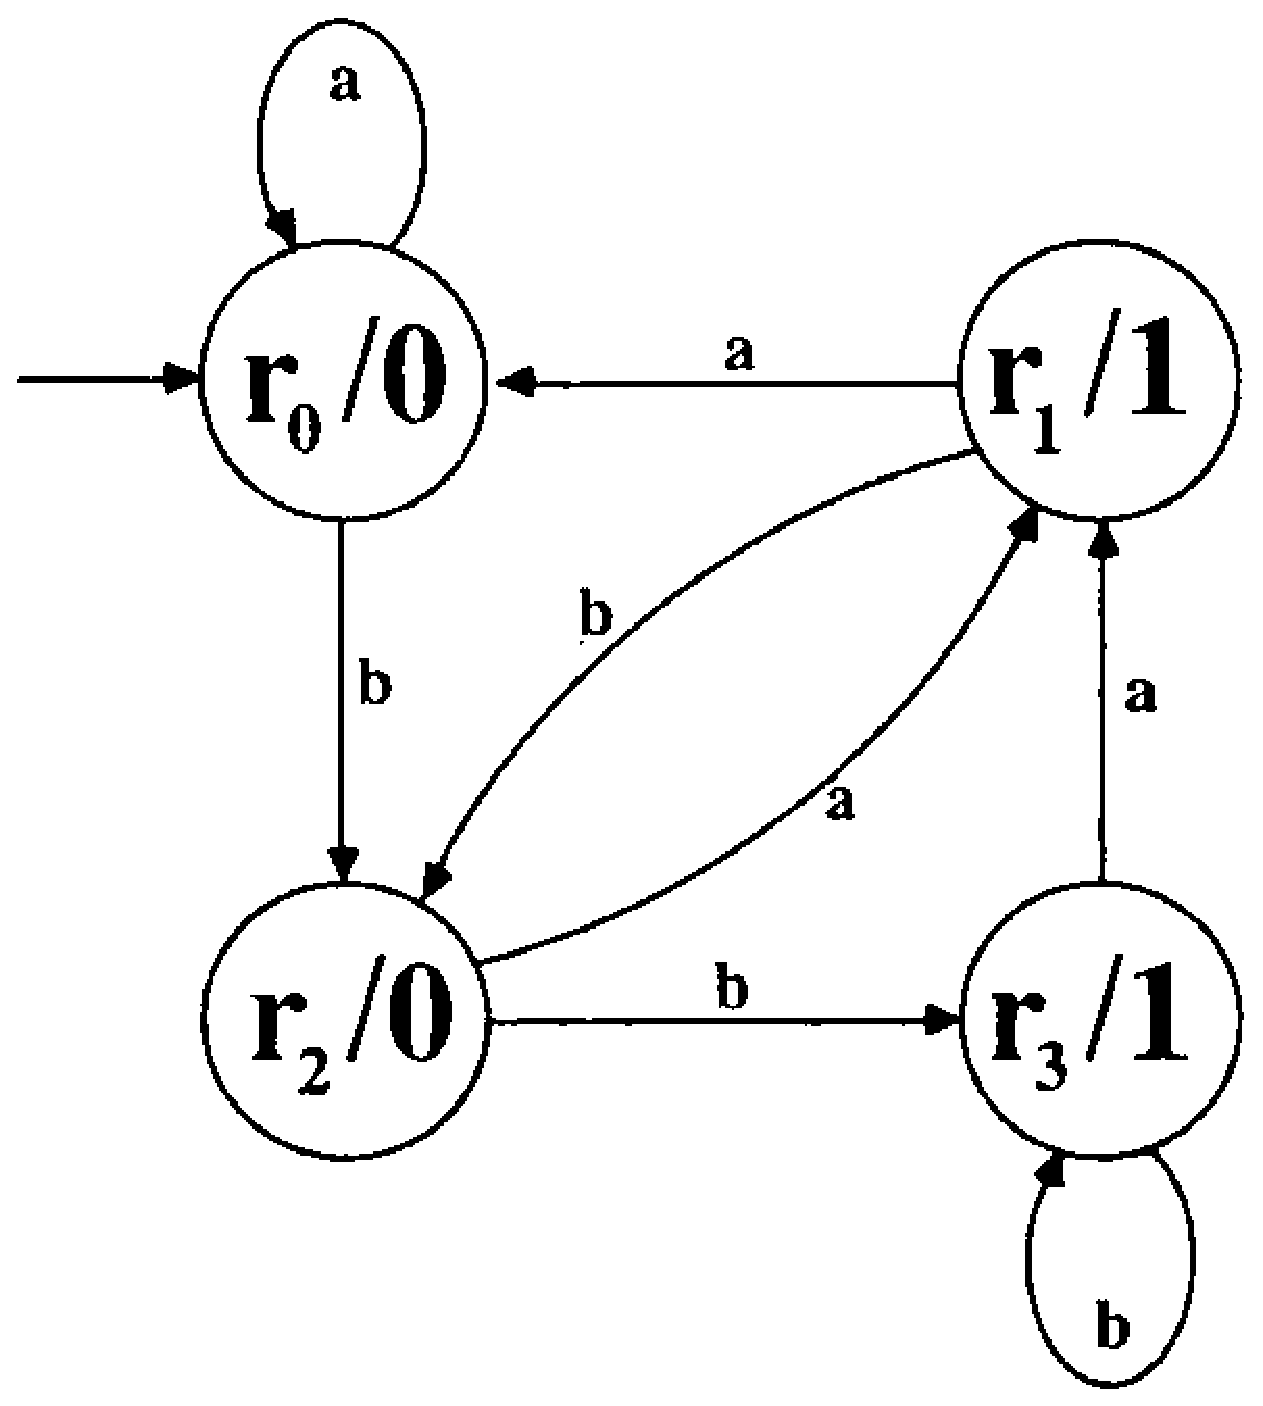
\epsfig{figure=ToFAfigures/fig7-6.eps,width=2.5in}}
\caption{The state transition diagram for the transducer discussed in Example
7.10}\label{fig-7.6}
\end{figure}

Results that were targeted toward a FST in the previous sections were specific
to Mealy machines. When the descriptor ``transducer'' appears in the theorems
and definitions presented earlier, the concept or result applies unchanged to
both FSTs and MSMs. Most of these results are alluded to but not restated in
this section. For example, \DBAR\ \index{extended state transition function \DBAR\! for MSM}
is defined like and behaves like the extended
state transition functions for DFAs and FSTs. On the other hand, because of the
drastic change in the domain of $\omega$, \OBAR\ must be modified as outlined
below in order for $\OBAR(s,x)$ to represent the output string produced when
starting at $s$ and processing $x$.

% Definition 7.17
\begin{dfn}\label{dfn-7.17}\index{extended output function \OBAR\! for MSM}
Given a MSM $A=\langle\Sigma,\Gamma,S,s_0,\delta,\omega\rangle$, the
\emph{\Index{extended output function}} for $A$, denoted again by \OBAR, is a
function $\omega$$: S \times \Sigma \rightarrow \Gamma^*$ defined recursively by:
\begin{enumerate}[i. ]
% handspaced vs. hardcoding i., ii.
\item $(\forall t \in S)\qquad\qquad\qquad\qquad\ \ \ \thinspace\thinspace\OBAR
	(t,\lambda)=\lambda$
\item $(\forall t \in S)(\forall x \in \Sigma^*)(\forall a \in \Sigma)
	(\OBAR(t,\pmb{a}x)=\omega(\delta(t,\pmb{a}))\cdot\OBAR
	(\delta(t,\pmb{a}),x)$
\end{enumerate}
\end{dfn}

Note that the domain of the function w has been extended further than usual:
in all previous cases, the domain was enlarged from $S \times \Sigma$ to
$S \times \Sigma^*$; in this instance, we are beginning with a domain of only
$S$ and still extending it to $S \times \Sigma^*$. The above definition allows
the following analog of Theorem \ref{thm-7.1} to remain essentially unchanged.

% Theorem 7.6
\begin{thm}\label{thm-7.6}
Let $\Sigma$ be an alphabet and $A=\langle\Sigma,\Gamma,S,s_0,\delta,\omega
\rangle$ be a Moore sequential machine. Then
\[ (\forall x \in \Sigma^*)(\forall y \in \Sigma^*)(\forall t \in S)(\OBAR(t,yx)
	=\OBAR(t,y) \cdot \OBAR(\DBAR(t,y),x)) \]
\emph{Proof.} The proof is by induction on $|y|$ (see the exercises and compare
with Theorem \ref{thm-1.1}).
\end{thm}

As before, the essence of a Moore machine is captured in the translation
function that the machine describes.

% Definition 7.18
\begin{dfn}\label{dfn-7.18}{\index{translation function!MSM}}
Given a MSM $M=\langle\Sigma,\Gamma,S,s_0,\delta,\omega\rangle$, the
\emph{translation function} for $M$, denoted by $f_M$, is the function
$f_M$$: \Sigma^* \rightarrow \Gamma^*$ defined by $f_M(x)=\OBAR(s_0,x)$.
\end{dfn}

Definition \ref{dfn-7.5} applies to Moore machines; two MSMs are equivalent if they
define the same translation. Indeed, it is possible for a Mealy machine to be
equivalent to a Moore machine, as shown by the transducers in Figures
\ref{fig-7.2} and \ref{fig-7.6}.

It is easy to turn a Moore machine $A=\langle\Sigma,\Gamma,S,s_0,\delta,\omega
\rangle$ into an equivalent Mealy machine $M=\langle\Sigma,\Gamma,S,s_0,\delta,
\omega'\rangle$. The first five parts of the transducer are unchanged. Only the
sixth component (the output function) must be redefined, as outlined below.

% Definition 7.19
\begin{dfn}\label{dfn-7.19}
Given a Moore machine $A=\langle\Sigma,\Gamma,S,s_0,\delta,\omega\rangle$, the
corresponding Mealy machine $M$ is given by $M=\langle\Sigma,\Gamma,S,s_0,
\delta,\omega'\rangle$, where $\omega'$ is defined by
\[ (\forall a \in \Sigma)(\forall s \in S)(\omega'(s,\pmb{a})=
	\omega(\delta(s,\pmb{a}))) \]
\end{dfn}

Pictorially, all arrows that lead \underline{into} a given state in the Moore machine should
be labeled in the corresponding Mealy machine with the output symbol for that
particular state. It follows easily from the definition that the corresponding
machines perform the same translation.

% Theorem 7.7
\begin{thm}\label{thm-7.7}\index{equivalent!transducers}
Given a Moore machine $A=\langle\Sigma,\Gamma,S,s_0,\delta,\omega\rangle$, the
corresponding Mealy machine\linebreak$M=\langle\Sigma,\gamma,S,s_0,\delta,\omega'\rangle$
is equivalent to $A$; that is, $(\forall x \in \Sigma^*)(f_M(x)=f_A(x))$.

\emph{Proof.} The proof is by induction on $|x|$ (see the exercises).
\end{thm}

\subsection*{Example 7.11}

Let $A=\langle\Sigma,\Gamma,S,r_0,\delta,\omega\rangle$ be the Moore machine
given in Figure \ref{fig-7.6}. The corresponding Mealy machine $M=\langle\Sigma,\Gamma,S,
s_0,\delta,\omega'\rangle$ is then given by
\[ \Sigma=\{\pmb{a},\pmb{b}\},\quad \Gamma=\{\pmb{0},\pmb{1}\},\quad
	S=\{r_0,r_1,r_2,r_3\},\quad s_0 = r_0 \]
and the state transition table and the output function table are specified as
in Tables 7.4a and 7.4b.
% Table 7.3a & 7.3b
\begin{table}[h]\label{table-7.3}
\begin{center}
\begin{tabular}{c|cc}
\multicolumn{3}{c}{Table 7.3a} \\
$\delta$ & $\pmb{a}$ & $\pmb{b}$ \\
\hline
$r_0$ & $r_0$ & $r_2$ \\
$r_1$ & $r_0$ & $r_2$ \\
$r_2$ & $r_1$ & $r_3$ \\
$r_3$ & $r_1$ & $r_3$
\end{tabular}
$\qquad$
\begin{tabular}{c|cc}
\multicolumn{3}{c}{Table 7.3b} \\
$\omega'$ & $\pmb{a}$ & $\pmb{b}$ \\
\hline
$r_0$ & $\pmb{0}$ & $\pmb{0}$ \\
$r_1$ & $\pmb{0}$ & $\pmb{0}$ \\
$r_2$ & $\pmb{1}$ & $\pmb{1}$ \\
$r_3$ & $\pmb{1}$ & $\pmb{1}$
\end{tabular}
\end{center}
\end{table}
The new Mealy machine is shown in Figure \ref{fig-7.7}. Note that the arrow labeled
$\pmb{a}$ leaving $r_1$ now has a $\pmb{0}$ associated with it, since the state at
which the arrow pointed $(r_0/\pmb{0})$ originally output a $\pmb{0}$.

% Figure 7.7
\begin{figure}
\centerline{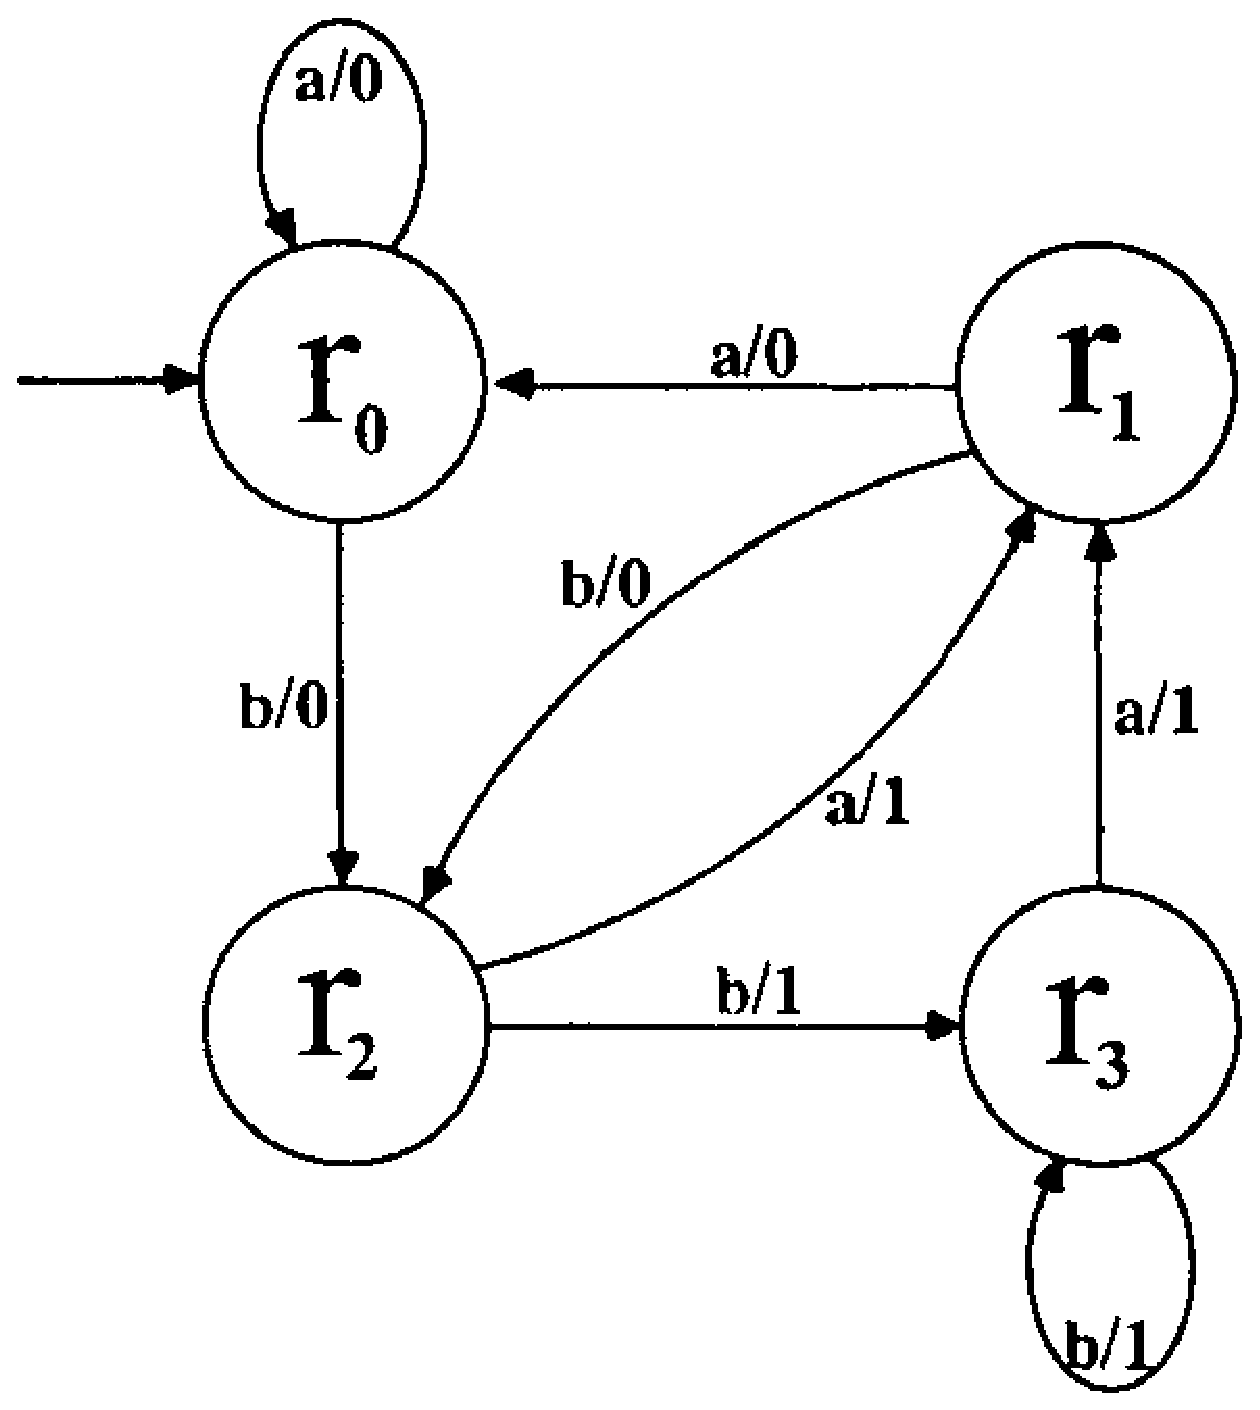
\epsfig{figure=ToFAfigures/fig7-7.eps,width=2.5in}}
\caption{The state transition diagram for the Mealy machine $M$ in Example 7.11}\label{fig-7.7}
\end{figure}

In a similar fashion, an equivalent Moore machine can be defined that
corresponds to a given Mealy machine. However, due to the more restricted nature
of the output function of the Moore constructs, the new machine will generally
need more states to perform the same translation.

The idea behind the construct is to break each state in the Mealy machine up
into a group of several similar states in the Moore machine, each of which
prints a different output symbol. The new transition function mimics the old
one; if state $r$ maps to state $t$ in the Moore machine, then any state in the
group corresponding to $r$ will map to one particular state in the group of
states corresponding to $t$. The particular state within the group is chosen in
a manner that will guarantee that the appropriate output symbol will be printed.
This construct is implemented in the following definition.

% Definition 7.20
\begin{dfn}\label{dfn-7.20}
Given a Mealy machine $M=\langle\Sigma,\Gamma,S,s_0,\delta,\omega\rangle$, the
corresponding Moore machine $A$ is given by $A=\langle\Sigma,\Gamma,S \times
\Gamma,\langle s_0,\alpha\rangle,\delta',\omega'\rangle$, where $\alpha$ is
an (arbitrary) member of\, $\Gamma$,
\[ \delta'\text{ is defined by }(\forall s \in S)(\forall\pmb{b}\in\Gamma)
	(\forall\pmb{a}\in\Sigma)(\delta'(\langle s,\pmb{b}\rangle, \pmb{a})
        =\langle\delta(s,\pmb{a}),\omega(s,\pmb{a})\rangle) \]
and
\[ \omega'\text{ is defined by }(\forall s \in S)(\forall\pmb{b}\in\Gamma)
	(\omega'(\langle s,\pmb{b}\rangle) = \pmb{b}). \]
\end{dfn}

% Theorem 7.8
\begin{thm}\label{thm-7.8}\index{equivalent!transducers}
Given a Mealy machine $M=\langle\Sigma,\Gamma,S,s_0,\delta,\omega\rangle$, the
corresponding Moore machine $A=\langle\Sigma,\Gamma,S,s_0,\delta',\omega'\rangle$
is equivalent to $M$; that is, $(\forall x \in \Sigma^*)(f_A(x)=f_M(x))$,

\emph{Proof.} The proof is by induction on $|x|$ (see the exercises).
\end{thm}

Since every Mealy machine has an equivalent Moore machine and every Moore
machine has an equivalent Mealy machine, either construct can be used as a
basis of what was meant by a translation $f$ being finite transducer definable.

% Corollary 7.8
\begin{cor}\label{cor-7.8}
A translation $J$ is FTD iff $f$ can be defined by a FST $M$ iff $f$ can be
defined by a MSM $A$.

\emph{Proof.} The proof is immediate from the definition of FTD and Theorems
\ref{thm-7.7} and \ref{thm-7.8}.
\end{cor}

\subsection*{Example 7.12}

Consider the Mealy machine $B$ from Figure \ref{fig-7.3}. The corresponding Moore machine
$A=\langle\Sigma,\Gamma,S,q_0,\delta,\omega\rangle$ is given by
\begin{center}\begin{tabular}{l}
$\Sigma=\{\pmb{a},\pmb{b}\}$ \\
$\Gamma=\{\pmb{0},\pmb{1}\}$ \\
$S=\{\langle s_0,\pmb{0}\rangle,\langle s_0,\pmb{1}\rangle,\langle s_1,\pmb{0}
	\rangle,\langle s_1,\pmb{1}\rangle\}$ \\
$q_0 = \langle s_0,\pmb{1}\rangle$ \\
$\omega(\langle s_0,\pmb{0}\rangle)=\pmb{0},\quad\omega(\langle s_0,\pmb{1}
	\rangle)=\pmb{1},\quad\omega(\langle s_1,\pmb{0}\rangle)=\pmb{0},\quad
	\omega(\langle s_1,\pmb{1}\rangle)=\pmb{1}$
\end{tabular}\end{center}
and the state transition table is specified as in Table 7.4.
% Table 7.4
\begin{table}[h]\label{tbl-7.4}
\begin{center}\begin{tabular}{c|cc}
\multicolumn{3}{c}{Table 7.4} \\
$\delta$ & $\pmb{a}$ & $\pmb{b}$ \\
\hline
$\langle s_0,\pmb{0}\rangle$ & $\langle s_0,\pmb{0}\rangle$ & $\langle s_1,
	\pmb{0}\rangle$ \\
$\langle s_0,\pmb{1}\rangle$ & $\langle s_0,\pmb{0}\rangle$ & $\langle s_1,
	\pmb{0}\rangle$ \\
$\langle s_1,\pmb{0}\rangle$ & $\langle s_0,\pmb{1}\rangle$ & $\langle s_1,
	\pmb{1}\rangle$ \\
$\langle s_1,\pmb{1}\rangle$ & $\langle s_0,\pmb{1}\rangle$ & $\langle s_1,
	\pmb{1}\rangle$
\end{tabular}\end{center}
\end{table}

% Figure 7.8
\begin{figure}
\centerline{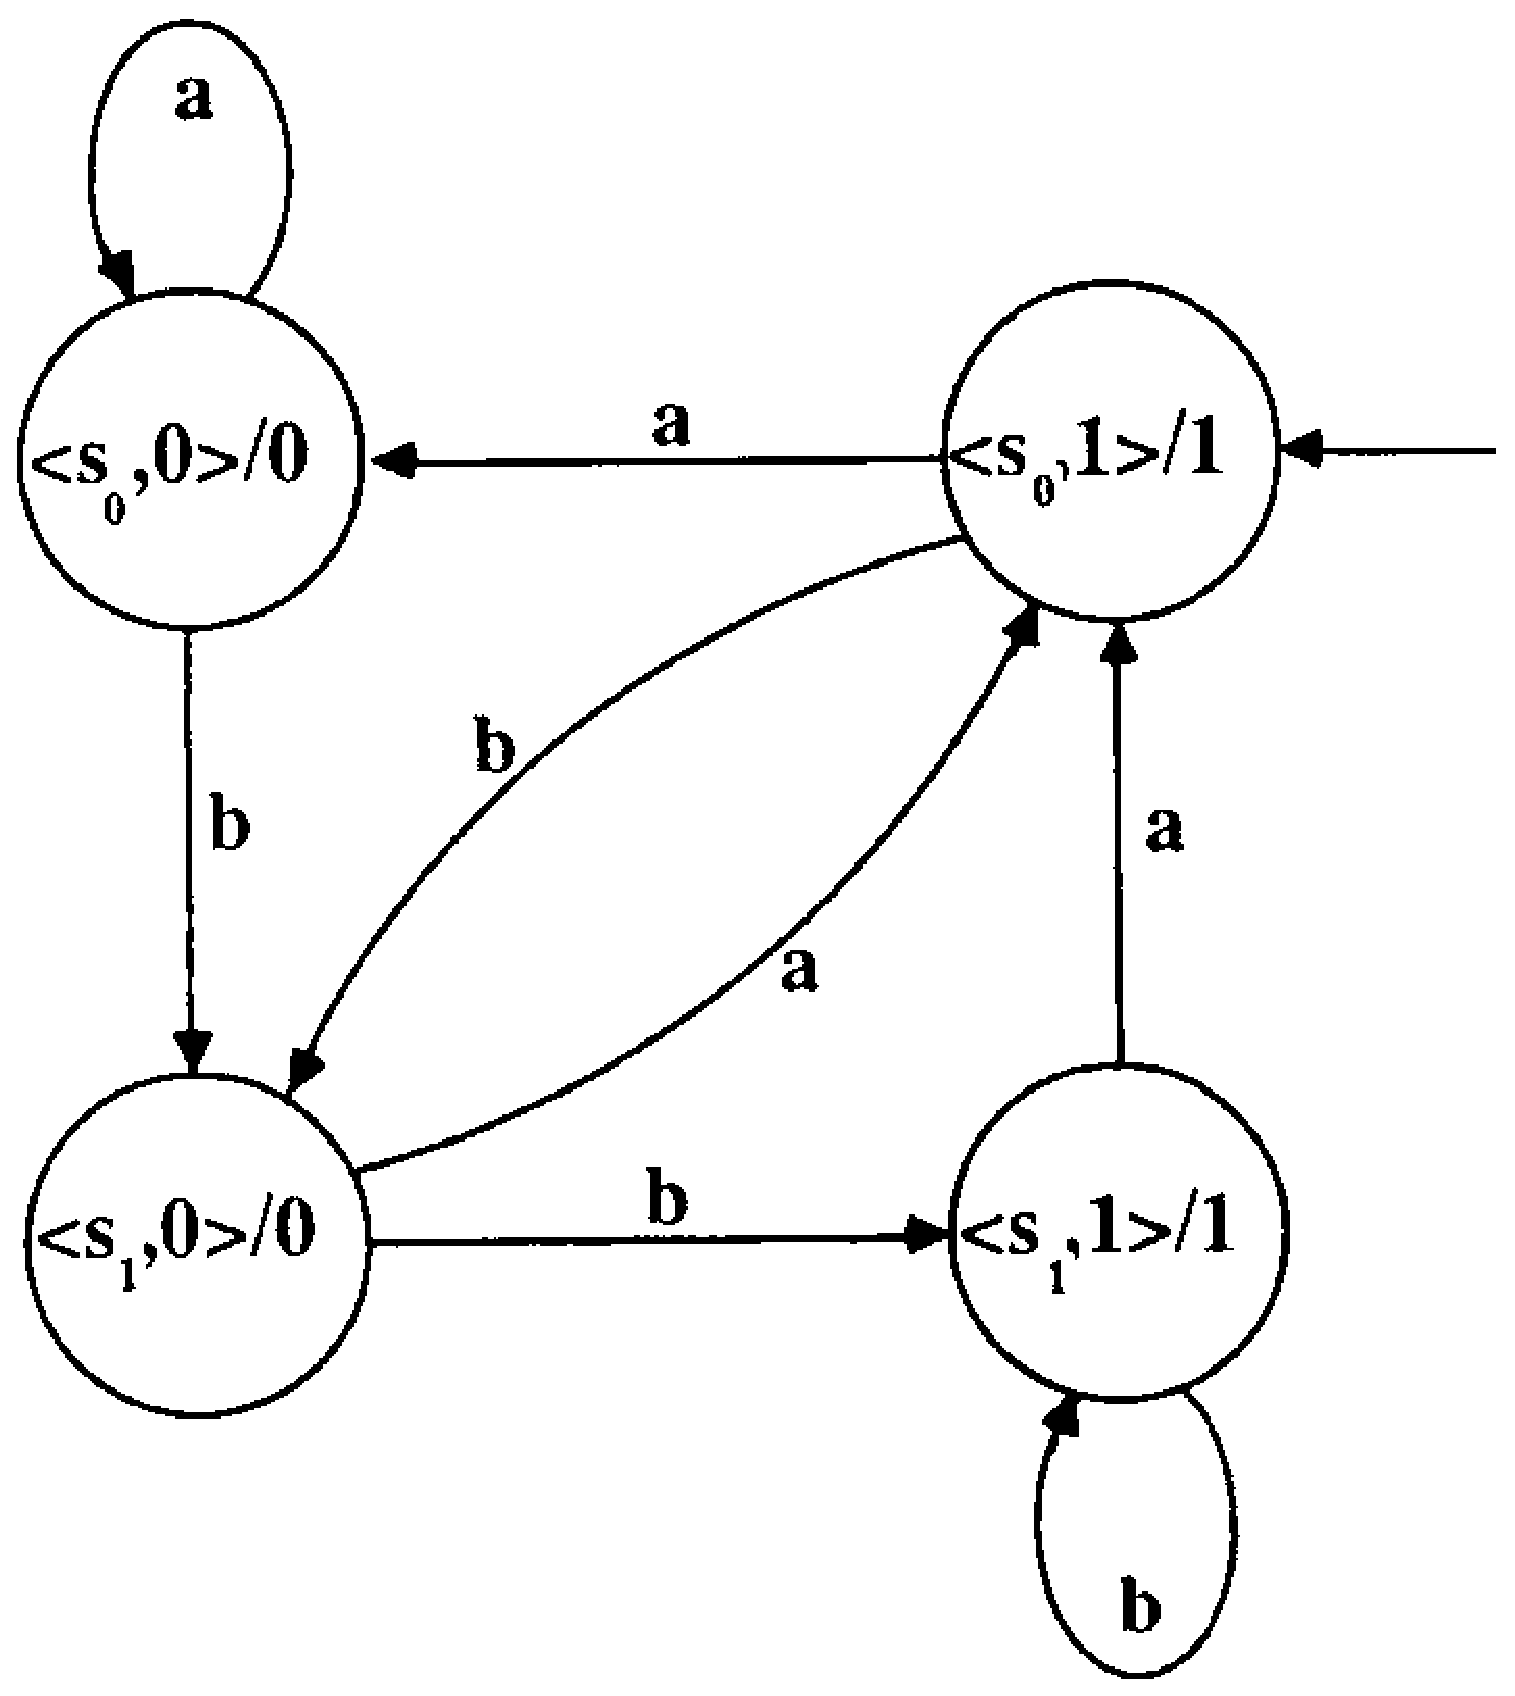
\epsfig{figure=ToFAfigures/fig7-8.eps,width=2.5in}}
\caption{The state transition diagram for the Moore machine A in Example
7.12}\label{fig-7.8}
\end{figure}

Figure \ref{fig-7.8} displays this new Moore machine. Note that this transducer $A$,
except for the placement of the start state, looks very much like the Moore
machine
$C$ given in Figure \ref{fig-7.6}. Indeed, any ordered pair that is labeled with the
original start state would be an acceptable choice for the new start state in
the corresponding Moore machine. For example, the automaton $A'$, which is
similar to $A$ but utilizes $\langle s_0,\pmb{0}\rangle$ as the new start state, is another
Moore machine that is equivalent to the original Mealy machine $B$. The
transition diagram for $A'$ is shown in Figure \ref{fig-7.9}. In fact, by appropriately
recasting the definition of isomorphism so that it applies to Moore sequential
machines, it can be shown that $A'$ and $C$ are isomorphic. The definition of
isomorphic again guarantees that a renaming of the states can be found that
preserves start states, transition functions, and output functions. Indeed, the
definition of isomorphism agrees with that of Mealy machines (and of DFAs, for
that matter) except in the specification of the correspondence between output
functions. The formal definition is given below.

% Figure 7.9
\begin{figure}
\centerline{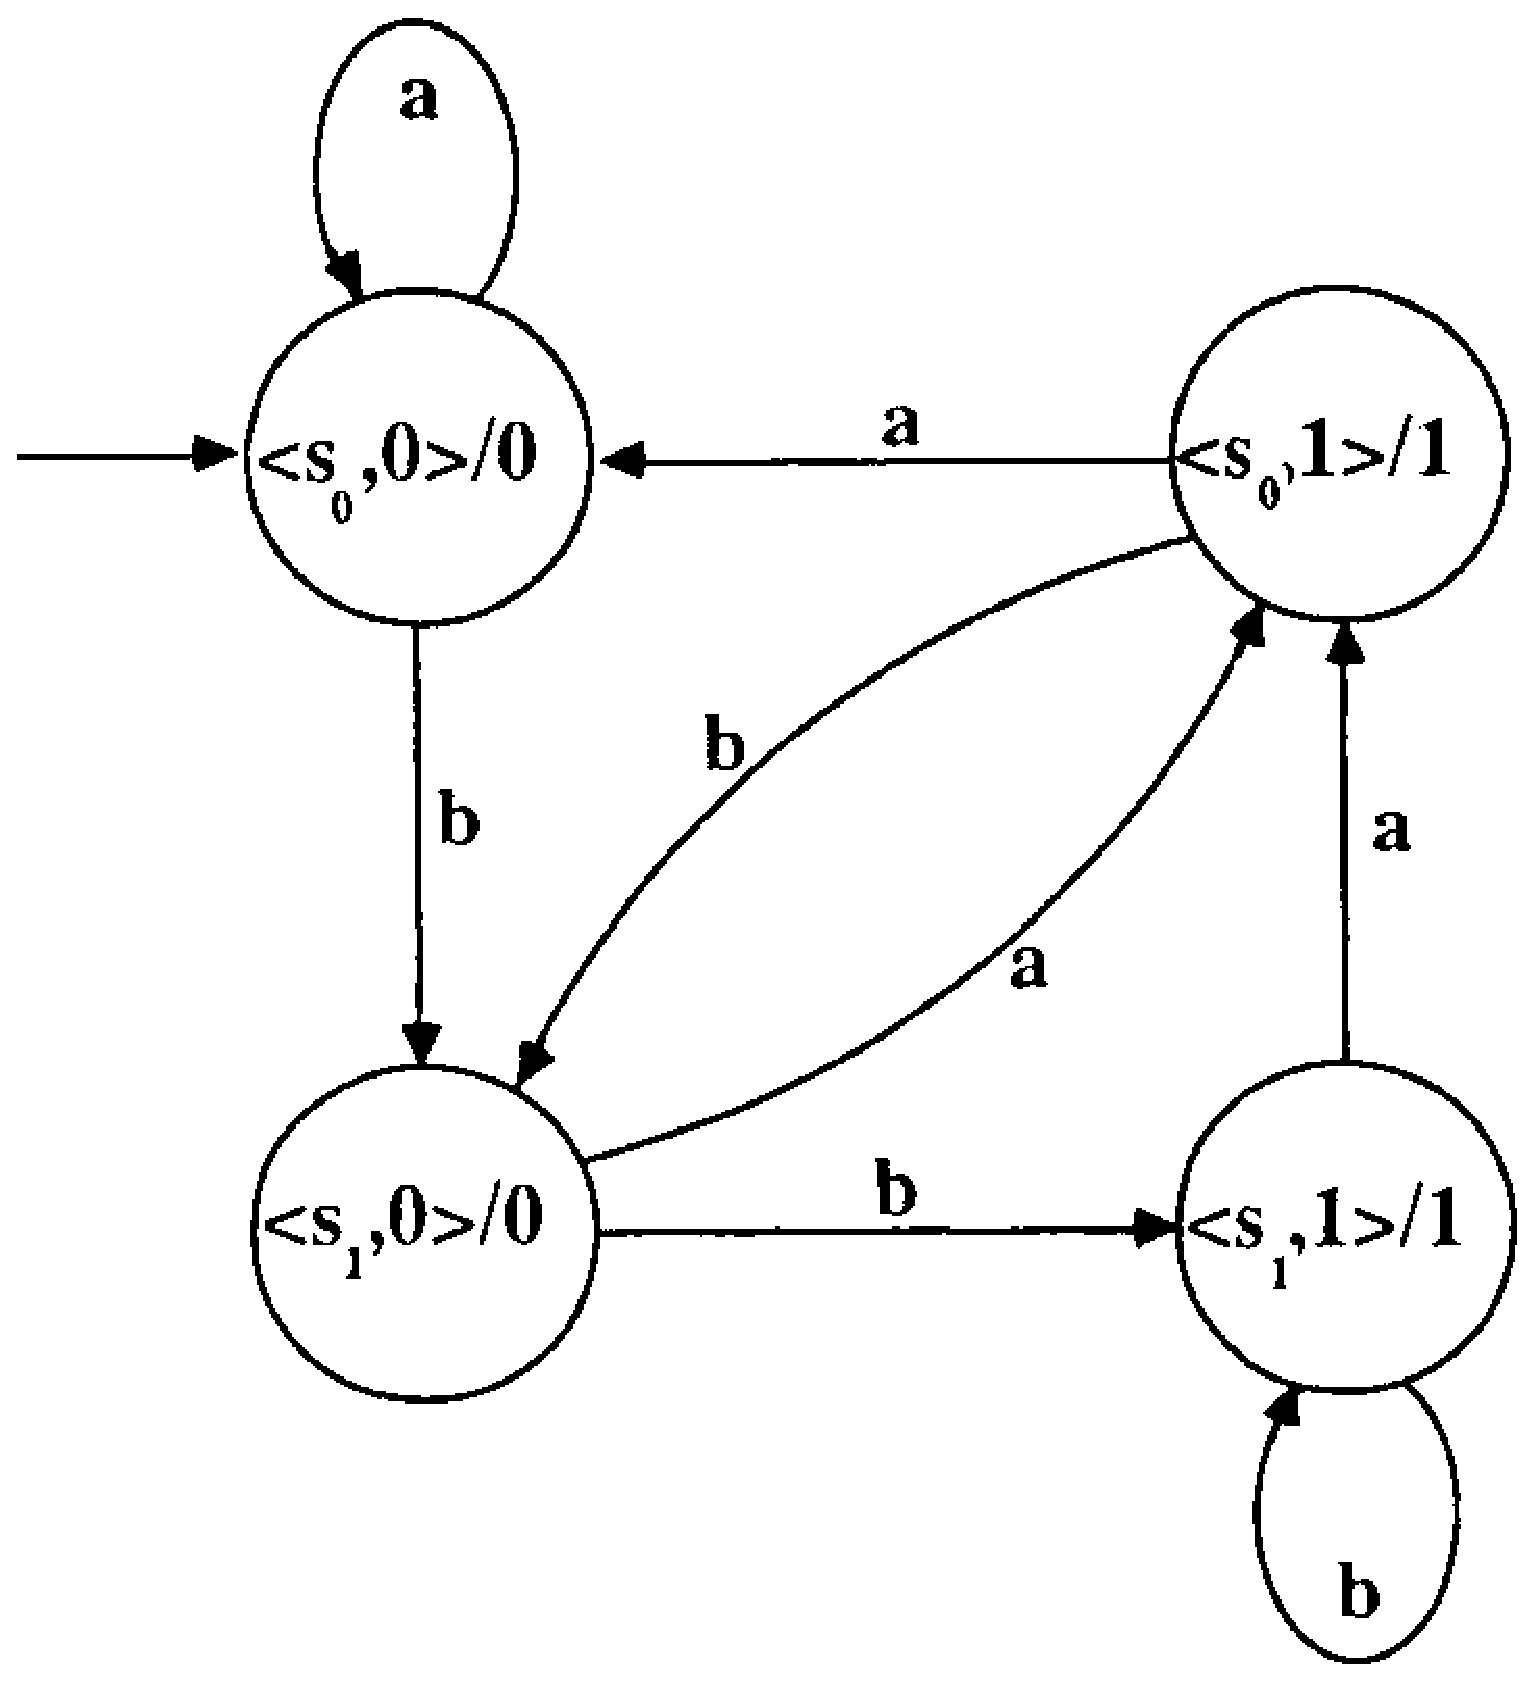
\epsfig{figure=ToFAfigures/fig7-9.eps,width=2.5in}}
\caption{The state transition diagram for the Moore machine $A'$ in Example
7.12}\label{fig-7.9}
\end{figure}

% Definition 7.21
\begin{dfn}\label{dfn-7.21}
Given two MSMs
\[ A=\langle\Sigma,\Gamma,S_A,s_{0_A},\delta_A,\omega_A\rangle\quad\text{ and }
	B=\langle\Sigma,\Gamma,S_B,s_{0_B},\delta_B,\omega_A\rangle, \]
and a function $\mu$$: S_A \rightarrow S_B,\ \mu$ is called a \emph{\Index{Moore
machine isomorphism}} from $A$ to $B$ iff the following five conditions hold:\emph{isomorphism}\index{isomorphism!between MSMs}
\begin{enumerate}[i.]
\item $\mu(s_{0_A}) = s_{0_B}$.
\item $(\forall s \in S_A)(\forall\pmb{a}\in\Sigma)(\mu(\delta_A(s,\pmb{a})) =
	\delta_B(\mu(s),\pmb{a}))$.
\item $(\forall s \in S_A)(\omega_A(s) = \omega_B(\mu(s)))$.
\item $\mu$ is a one-to-one function between $S_A$ and $S_B$.
\item $\mu$ is onto $S_B$.
\end{enumerate}
\end{dfn}

\subsection*{Example 7.13}

The two Moore machines $A'$ in Figure \ref{fig-7.9} and $C$ in Figure \ref{fig-7.6} are indeed
\Index{isomorphic}. There is a function $\mu$ from the states of $A'$ to the states of
$C$ that satisfies all five properties of an isomorphism. This correspondence is
given by $\mu(\langle s_0,\pmb{0}\rangle) = r_0,\ \mu(\langle s_0,\pmb{1}\rangle)
=r_1,\ \mu(\langle s_1,\pmb{0}\rangle)=r_2$, and $\mu(\langle s_1,\pmb{1}\rangle)=r_3$,
succinctly defined by $\mu(\langle s_i,j\rangle)=r_{2i+j}$, for $i,j \in
\{\pmb{0},\pmb{1}\}$. As before, a homomorphism is meant to represent a
correspondence between states that preserves the algebraic structure of the
transducer without necessarily being a bijection.

% Definition 7.22
\begin{dfn}\label{dfn-7.22}
Given two MSMs
\[ A=\langle\Sigma,\Gamma,S_A,s_{0_A},\delta_A,\omega_A\rangle\quad\text{ and }
	B=\langle\Sigma,\Gamma,S_B,s_{0_B},\delta_B,\omega_A\rangle, \]
and a function $\mu$$: S_A \rightarrow S_B,\ \mu$ is called a \emph{\Index{Moore
machine homomorphism}} from $A$ to $B$ iff the following three conditions hold:
\index{homomorphism!between MSMs}

\begin{enumerate}[i.]
\item $\mu(s_{0_A}) = s_{0_B}$.
\item $(\forall s \in S_A)(\forall\pmb{a}\in\Sigma)(\mu(\delta_A(s,\pmb{a})) =
	\delta_B(\mu(s),\pmb{a}))$.
\item $(\forall s \in S_A)(\omega_A(s) = \omega_B(\mu(s)))$.
\end{enumerate}
\end{dfn}

The isomorphism $\mu$ discussed in Example 7.13 is also a homomorphism.
Preserving the algebraic structure of the transducer guarantees that the
translation is also preserved: if $A$ and $B$ are homomorphic, then they are
equivalent. The homomorphism criterion that applies to single letters once again
extends to similar statements about strings, as outlined in Lemma \ref{lmm-7.5}.

% Lemma 7.5
\begin{lmm}\label{lmm-7.5}
If $\mu$$: S_A \rightarrow S_B$ is a homomorphism between two MSMs
\[ A=\langle\Sigma,\Gamma,S_A,s_{0_A},\delta_A,\omega_A\rangle\quad\text{ and }
	B=\langle\Sigma,\Gamma,S_B,s_{0_B},\delta_B,\omega_A\rangle, \]
then
\[ (\forall s \in S_A)(\forall x \in \Sigma^*)(\mu(\DBAR_A(s,x))=\DBAR_B
	(\mu(s),x)) \]
and
\[ (\forall s \in S_A)(\forall x \in \Sigma^*)(\OBAR_A(s,x)=\OBAR_B
	(\mu(s),x)). \]
\emph{Proof.} The proof is by induction on $|x|$ (see the exercises).
\end{lmm}

% Corollary 7.9
\begin{cor}\label{cor-7.9}
If $\mu$$:S_A \rightarrow S_B$ is a homomorphism between two MSMs
$A=\langle\Sigma,\Gamma,S_A,s_{0_A},\delta_A,\omega_A\rangle$ and
$B=\langle\Sigma,\Gamma,S_B,s_{0_B},\delta_B,\omega_B\rangle$, then $A$ is
equivalent to $B$; that is, $f_A = f_B$.

\emph{Proof.} The proof follows immediately from Lemma \ref{lmm-7.5} and the definition
of $f_M$.
\end{cor}

It is interesting to note that the MSMs $A$ in Figure \ref{fig-7.8} and $A'$ in Figure
\ref{fig-7.9} are not isomorphic. In fact, there does not even exist a homomorphism (in
either direction) between $A$ and $A'$ since the start states print different
symbols, and rules (i) and (iii) therefore conflict. The absence of an
isomorphism in this instance illustrates that an analog to Theorem \ref{thm-7.5} cannot be
asserted under the definition of Moore sequential machines presented here.
Observe that $A$ and $A'$ are equivalent and they are both minimal (four states
are necessary in a Moore machine to perform this translation), yet they are not
isomorphic. The reader should contrast this failure with the analogous statement
about Mealy machines in Theorem \ref{thm-7.5}.

Producing a result comparable to Theorem \ref{thm-7.5} is not possible without a
fundamental adjustment of at least one of the definitions. One possibility is to
drop the distinguished start state from the definition of the Moore machine.
This removes condition (i) from the isomorphism definition and thereby resolves
the conflict between (i) and (iii). We have already noted that many applications
do not require a distinguished start state (such as elevators and traffic signal
controls), which makes this adjustment not altogether unreasonable.

A more common alternative is to decree that a Moore sequential machine first
print the character specified by the start state upon being turned on (before
any of the input tape is read) and then proceed as before. This results in
output strings that are always one symbol longer than the corresponding input
strings, and the length-preserving property of transducers is thereby lost. A
more substantial drawback results from the less natural correspondence between
Mealy and Moore machines: no FST can be truly equivalent to any MSM since
translations would not even be of the same length.

The advantage of this decree is that machines like $A$ and $A'$ (from Figures
\ref{fig-7.8} and \ref{fig-7.9}) would no longer be equivalent, and hence they would not be expected
to be isomorphic. Note that equivalence is lost since, under the new decree for
translations, they would produce different output when presented with, say,
$\lambda$ as input: $A$ would print $\pmb{1}$ while $A'$ would produce
$\pmb{0}$. Our definition of a MSM (Definition \ref{dfn-7.16}) was chosen to remain
compatible with the translations obtained from Mealy machines and to preserve a
distinguished state as the start state; these advantages were obtained at the
expense of a convenient analog to Theorem \ref{thm-7.5}.

A third, and perhaps the best, alternative is to modify what we mean by a MSM
isomorphism. Definition \ref{dfn-7.21} can be rephrased to relax the condition that the
start states of the two machines must print the same character.

As with Mealy machines, Moore machines can also be minimized, and a reduced and
connected MSM is guaranteed to be the smallest MSM which performs that
translation. Note that Definitions \ref{dfn-7.4} (FTD), \ref{dfn-7.5} (equivalence), \ref{dfn-7.9}
(isomorphic), \ref{dfn-7.10} (connected), \ref{dfn-7.12} (state equivalence relation), \ref{dfn-7.13}
(reduced), and \ref{dfn-7.15}\index{equivalent!MSM states} ($i^{\text th}$ relation) have been phrased to encompass both forms
of transducers. Minor changes (generally involving the domain of the output
function) are all that is necessary to make the remaining definitions and
results conform to the Moore constructs. We begin with a formal definition of
minimality, which is in essence the same as the definitions presented for DFAs
and FSTs (Definitions \ref{dfn-2.7} and \ref{dfn-7.6}).

% Definition 7.23
\begin{dfn}\label{dfn-7.23}
Given a MSM $A=\langle\Sigma,\Gamma,S_A,s_{0_A},\delta_A,\omega_A\rangle,\ A$ is
the \emph{\Index{minimal Moore machine} for the translation} $f_A$ iff for all MSMs
$B=\langle\Sigma,\Gamma,S_B,s_{0_B},\delta_B,\omega_B\rangle$ for which
$f_A = f_B,\ \|S_A\| \leq \|S_B\|$.
\end{dfn}

A connected Moore machine is essential to minimality. The previous definition
of connectedness (Definition \ref{dfn-7.10}) suffices for both FSTs and MSMs and was
therefore phrased to apply to all transducers, rather than to one specific
type of transducer. For an arbitrary Moore machine, the algorithm for finding
the set of accessible states is unchanged; transitions are followed from the
start state until no further new states are found. The connected version of a
MSM is again obtained by paring down the state set to encompass only the
connected states and restricting the $\delta$ and $\omega$ functions to the
smaller domain.

% Definition 7.24
\begin{dfn}\label{dfn-7.24}\index{M connected (MSM $M^c$)}\index{A@$A^c$ (A connected)!for MSM}
Given a MSM $M=\langle\Sigma,\Gamma,S,s_0,\delta,\omega\rangle$, define the
transducer $M^c =\langle\Sigma,\Gamma,S^c,s^c_0,\delta^c,\omega^c\rangle$,
called \emph{M connected}, by
\begin{center}\begin{tabular}{l}
$S^c=\{s \in S^c$ $|$ $\exists x \in \Sigma^* \ni \DBAR(s_0,x) = s\}$ \\
$s^c_0 = s_0$
\end{tabular}\end{center}
$\delta^c$ is essentially the restriction of $\delta$ to $S^c \times \Sigma:\ 
(\forall\pmb{a}\in\Sigma)(\forall s \in S^c)(\delta^c(s,\pmb{a}) = 
\delta(s,\pmb{a}))$, and $\omega^c$ is the restriction of $\omega$ to
$S^c \times \Sigma:\ (\forall s \in S^c)(\omega^c(s) = \omega(s))$.
\end{dfn}

The concept of a reduced Moore machine and the definition of the state
equivalence relation are identical in spirit and in form to those presented
for Mealy machines (Definitions \ref{dfn-7.12} and \ref{dfn-7.13}). The definition that outlines
how to reduce a Moore machine by coalescing states differs from that given for
FSTs (Definition \ref{dfn-7.14}) only in the specification of the output function. In
both Definition \ref{dfn-7.14} and the following Moore machine analog, the value $\omega$
takes for an equivalence class is determined by the value given for a
representative of that equivalence class. As before, this natural definition for
the output function can be shown to be well defined (see the exercises).

% Definition 7.25
\begin{dfn}\label{dfn-7.25}\index{A @$ A/_{E_A}$ (A modulo $E_A$)!for MSM}
Given a MSM $M=\langle\Sigma,\Gamma,S,s_0,\delta,\omega\rangle$, define
\Index{M$/\!\!_{E_M}$}, \emph{$M$ modulo its state equivalence relation}, by
$M/\!\!_{E_M}=\langle\Sigma,\Gamma,S_{E_M},s_{0_{E_M}},\delta_{E_M},\omega_{E_M}
\rangle$, where
\begin{center}\begin{tabular}{l}
$S_{E_M}=\{[s]_{E_M}$ $|$ $ s \in S\}$ \\
$s_{0_{E_M}} = [s_0]_{E_M}$
\end{tabular}\end{center}
$\delta_{E_M}$ is defined by
\[ (\forall\pmb{a}\in\Sigma)(\forall [s] \in S_{E_M})(\delta_{E_M}
	([s]_{E_M},\pmb{a})=[\delta(s,\pmb{a})]_{E_M}), \]
and $\omega_{E_M}$ is defined by
\[ (\forall [s] \in S_{E_M})(\omega_{E_M}([s]_{E_M}) = \omega(s)) \]
\end{dfn}

The Moore machine $M/\!\!_{E_M}$ has all the properties attributed to the Mealy
version. Without changing the nature of the translation, it is guaranteed to
produce a MSM which is reduced.

% Theorem 7.9
\begin{thm}\label{thm-7.9}
Given a MSM $M=\langle\Sigma,\Gamma,S,s_0,\delta,\omega\rangle$:
\begin{enumerate}[a.]
\item $M/\!\!_{E_M}=\langle\Sigma,\Gamma,S_{E_M},s_{0_{E_M}},\delta_{E_M},
	\omega_{E_M}\rangle$ is equivalent to $M$.
\item $M/\!\!_{E_M}$ is reduced.
\item If $M$ is connected, so is $M/\!\!_{E_M}$.
\item Given a FTD function $f$, the minimal Moore machine corresponding to $f$
must be reduced.
\end{enumerate}

\emph{Proof.} The proof is similar to Theorem \ref{thm-7.4} (see the exercises).
\end{thm}

As mentioned earlier, the definition of a MSM chosen here denies a convenient
analog to Theorem \ref{thm-7.5}. However, a reduced and connected Moore machine must be
minimal.

% Theorem 7.10
\begin{thm}\label{thm-7.10}
\item Given a MSM $M$:
\begin{enumerate}[(a)]
\item
A necessary and sufficient condition for $M$ to be
	minimal is that $M$ is both reduced and connected.
\item $M^c\!/\!\!_{E_{M^c}}$, is minimal.
\end{enumerate}

\emph{Proof.} See the exercises.
\end{thm}

The minimal Moore machine corresponding to a MSM $M$ can thus be obtained
if the connected state set and the state equivalence relation can be computed.
The algorithm for calculating the accessible states is the same as before, and
computing the state equivalence relation will again be accomplished using the
concept of the $i$th state equivalence relation (Definition \ref{dfn-7.15}). All the
results proved previously in Lemma \ref{lmm-7.3} still hold, showing that successive
calculations are guaranteed to halt and produce $E_M$. All that remains is to
specify both a starting point and a way to find the next relation from the
current $E_{iM}$.

With Mealy machines, $E_{0M}$ consisted of one single equivalence class, since
$\lambda$ could not distinguish between states. All states were therefore
related to each other under $E_{0M}$. With Moore machines, different states
cause different letters to be printed. $E_{0M}$ can therefore be thought of as
grouping together states that print the same symbol.

% Lemma 7.6
\begin{lmm}\label{lmm-7.6}
Given a MSM $M=\langle\Sigma,\Gamma,S,s_0,\delta,\omega\rangle$:
\begin{enumerate}[(a)]
\item $E_{0M}$ is defined by $s E_{0M} t \Leftrightarrow (\omega(s)=\omega(t))$.
\item For $i \geq 0$, $E_{i+1M}$ can be computed from $E_{iM}$ as follows:
\[ (\forall s \in S)(\forall t \in S)(\forall i \geq 0)(s E_{i+1M} t
	\Leftrightarrow s E_{iM} t \wedge (\forall\pmb{a}\in\Sigma)
	(\delta(s,\pmb{a})E_{iM}\delta(t,\pmb{a}))). \]
\end{enumerate}

\emph{Proof.} The proof is essentially the same as in Chapter \ref{ch-3} (see Theorem
\ref{thm-3.8}).
\end{lmm}

% Corollary 7.10
\begin{cor}\label{cor-7.10}
Given a MSM $M=\langle\Sigma,\Gamma,S,s_0,\delta,\omega\rangle$, there is an
\emph{algorithm} for computing $E_M$.

\emph{Proof.} See the exercises.
\end{cor}

$E_{0M}$ will generally have one equivalence class for each symbol in $\Gamma$;
$rk(E_{0M})$ could be less than $\|\Gamma\|$ if some output symbols are not
printed by any state (remember that equivalence classes are by definition
nonempty). The rule for computing $E_{i+1M}$ from $E_{iM}$ is identical to that
given for Mealy machines (and DFAs); only the starting point, $E_{0M}$, had to
be redefined for Moore machines (compare with Lemma \ref{lmm-7.4}). Lemmas \ref{lmm-7.3} and \ref{lmm-7.6}
imply that there is an algorithm for finding $E_M$ for any Moore machine $M$;
this was the final computation needed to produce $M^c\!/\!\!_{E_{M^c}}$, which will be
the minimal Moore machine equivalent to the MSM $M$.

% Corollary 7.11
\begin{cor}\label{cor-7.11}
Given a MSM $M=\langle\Sigma,\Gamma,S,s_0,\delta,\omega\rangle$, there is an
\emph{algorithm} for computing the minimal machine equivalent to M.

\emph{Proof.} See the exercises.
\end{cor}

\section{Transducer Applications and Circuit Implementation}\label{7.4}

The vending machine example that began this chapter showed that the transducer
was capable of modeling many of the machines we deal with in everyday life. This
section gives examples of several types of applications and then shows how to
form the circuitry that will implement such transducers. Transducers can be used
not only to model physical machinery, but can also form the basis for
computational algorithms. The following example can be best thought of not as a
model of a machine that receives files, but as a model of the behavior of the
computer algorithm that specifies how such files are to be received.

\subsection*{Example 7.14}

The transducer metaphor is often used to succinctly describe the structure of
many algorithms commonly used in computer applications, most notably in network
communications. \emph{Kermit}\index{Kermit protocol!FST implementation} is a popular means of transferring files
between mainframes and microcomputers. A transfer is accomplished by the send
portion of Kermit on the source host exchanging information with the receive
portion of Kermit on the destination host. The two processes communicate by
exchanging \emph{packets} of information; these packets comprise the input
alphabet of our model. When the Kermit protocol was examined in Chapter \ref{ch-1}
(Example 1.16), it was noted that a full description of the algorithm must also
describe the action taken upon receipt of an incoming packet; these actions
comprise the output alphabet of our model. During a file transfer, the states of
the receiving portion of Kermit on the destination host are $R$ (awaiting a
transfer request), $RF$ (awaiting the name of the file to be transferred),
$RD$ (awaiting more data to be placed in the new file), and $A$ (abort due to an
unrecoverable error). The set of states will again be $A,R,RD,RF\}$.

Expected inputs are represented by  $\pmb{S}$ (an initialization packet, indicating
that a transfer is requested), $\pmb{H}$ (a header packet, containing the name of
one of the files to be created and opened), $\pmb{D}$ (a data packet), $\pmb{Z}$ (an
end of file marker [\Index{EOF packet}], signaling that no more data need be placed in the currently
opened file), and $\pmb{B}$ (break, signaling the end of transmission). Unexpected
input, representing a garbled transmission, is denoted by $\pmb{X}$. The input
alphabet is therefore $\Sigma=\{\pmb{B},\pmb{D},\pmb{H},\pmb{S},\pmb{X},
\pmb{Z}\}$.

When Kermit receives a recognizable packet [that is also appropriate at the
current stage of the conversation], it sends an acknowledgment (ACK)
back to the other host. This action will be represented in the output alphabet
by the symbol $\pmb{Y}$. When the receiver expects and gets a valid header packet,
it opens the appropriate file and also acknowledges the packet. This pair of
actions is represented by the output symbol $\pmb{O}$. $\pmb{W}$ will denote the
writing of the packet contents to the opened file and acknowledgment of the
packet, and $\pmb{\varphi}$ will denote that no action is taken. $\pmb{C}$ will
indicate that the currently opened file is closed. $\pmb{N}$ will represent the
transmission of a NAK (negative acknowledgment, essentially a request to resend
the contents of the previous packet), which is used to alert the
sender that a garbled packet was detected. The output alphabet is therefore
$\Gamma=\{\pmb{N},\pmb{O},\pmb{W},\pmb{Y},\pmb{\varphi}\}$. The complete
algorithm is summed up in the state transition diagram given in Figure \ref{fig-7.10}.

Hardware as well as software can be profitably modeled by finite-state
transducers. The column-by-column addition of two binary numbers is quite
naturally modeled by a simple two-state FST, since the carry bit is the only
piece of previous history needed by the transducer to correctly sum the current
column. This discussion will focus on binary numbers in order to keep the
alphabets small, but trivial extensions will make the two-state machine apply to
addition in any base system.

% Figure 7.10
\begin{figure}
\centerline{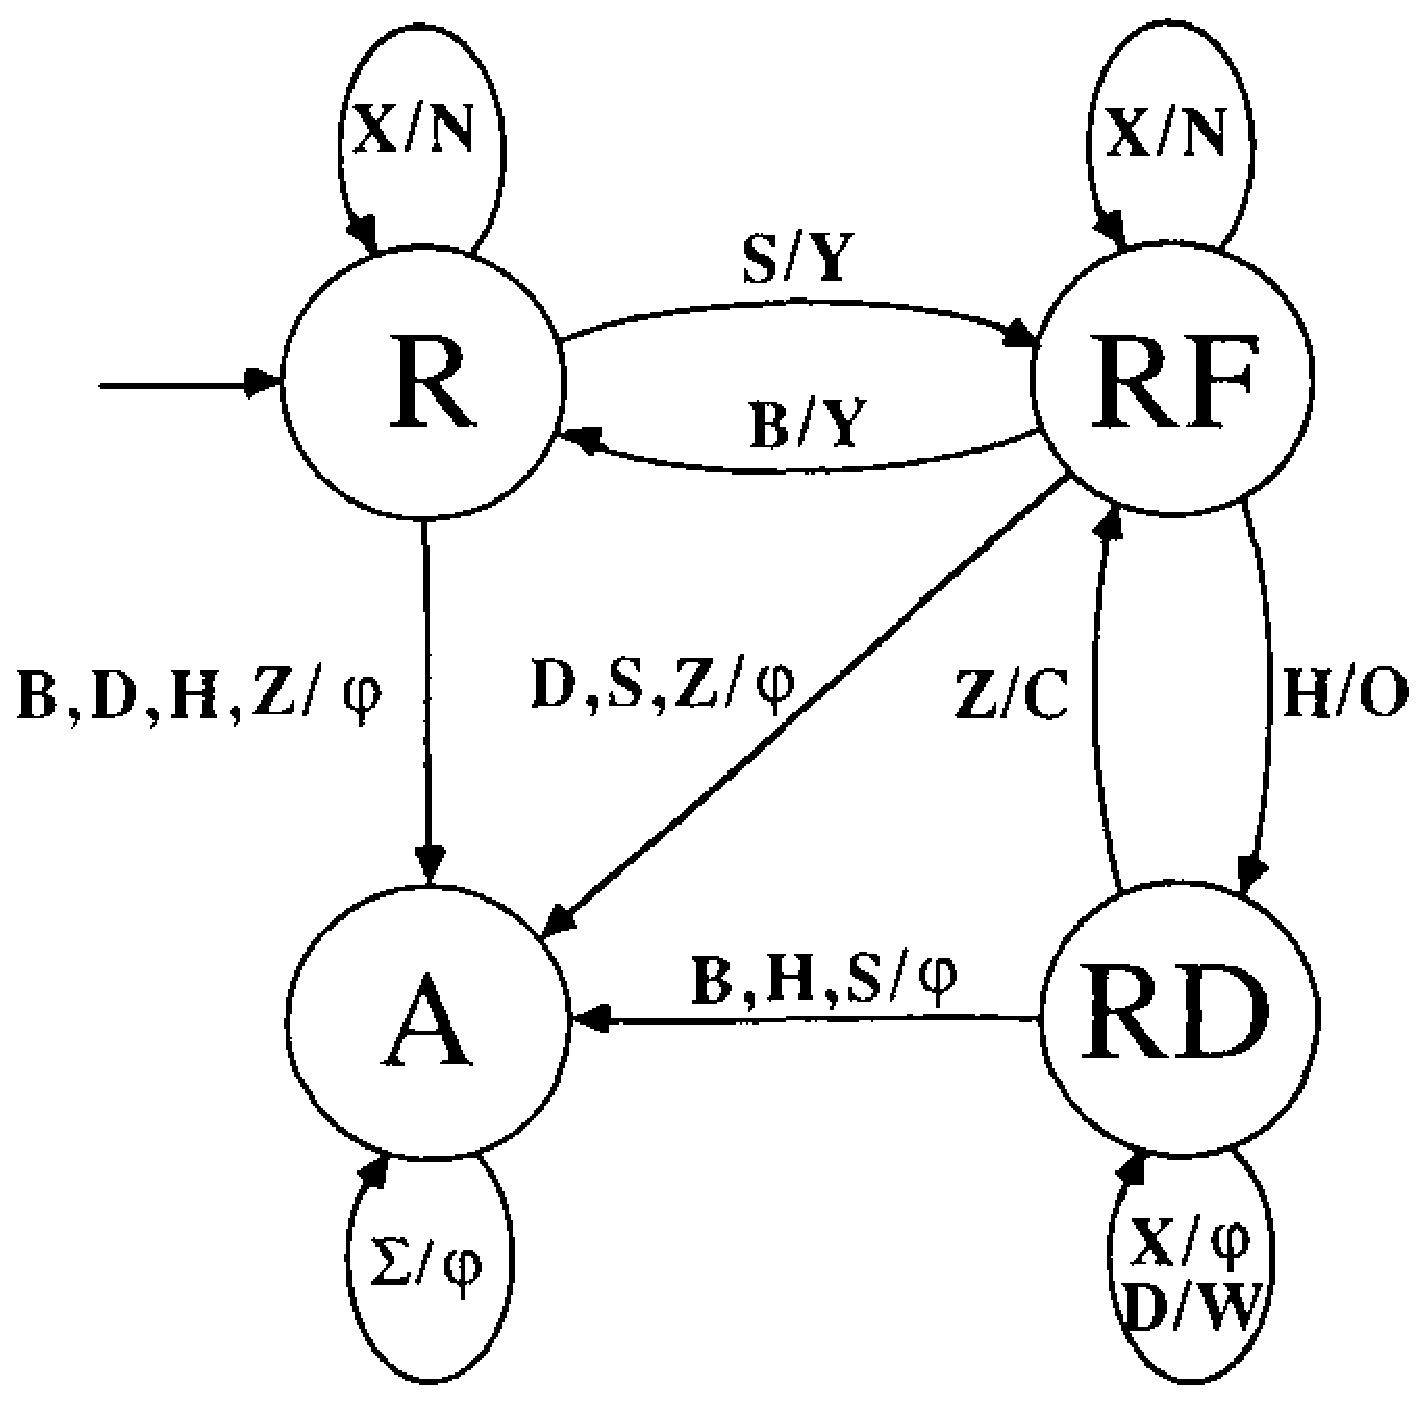
\epsfig{figure=ToFAfigures/fig7-10.eps,width=2.5in}}
\caption{The state transition diagram for the receive portion of Kermit, as
discussed in Example 7.14}\label{fig-7.10}
\end{figure}

\subsection*{Example 7.15}\index{addition automaton (FST)}

A computation such as the one shown in Figure \ref{fig-7.11}a would be divided up into
columns and presented to the FST as indicated in Figure \ref{fig-7.11}b (shown in
mid-computation). A digit from the first number and the corresponding digit from
the second number are presented to the transducer as a single input symbol. With
the column pairs represented by standard ordered pairs, the corresponding input
might appear as in Figure \ref{fig-7.12} (shown at the start of computation). As
illustrated by the orientation of the tape, this FST must be set up to process
strings \emph{in reverse}, that is, from right to left, since computations must
start with the low-order bits to ensure that the correct answer is always
(deterministically) computed. With states $C$ (representing carry) and $N$ (no
carry), input alphabet\index{binary alphabet} $\Sigma=\{\langle 0,0\rangle,\langle 0,1\rangle,\langle
1,0\rangle,\langle 1,1\rangle\}$ and output alphabet $\Gamma=\{\pmb{0},
\pmb{1}\}$, this binary adder behaves as shown in the state transition diagram
given for $B$ in Figure \ref{fig-7.13}. For the problem displayed in Figure \ref{fig-7.11}a, the
output produced by $B$ would be $\pmb{01001}$ (9 in binary), which is the
appropriate translation of the addition problem given ($6+3$).

% Figure 7.11
\begin{figure}
\centerline{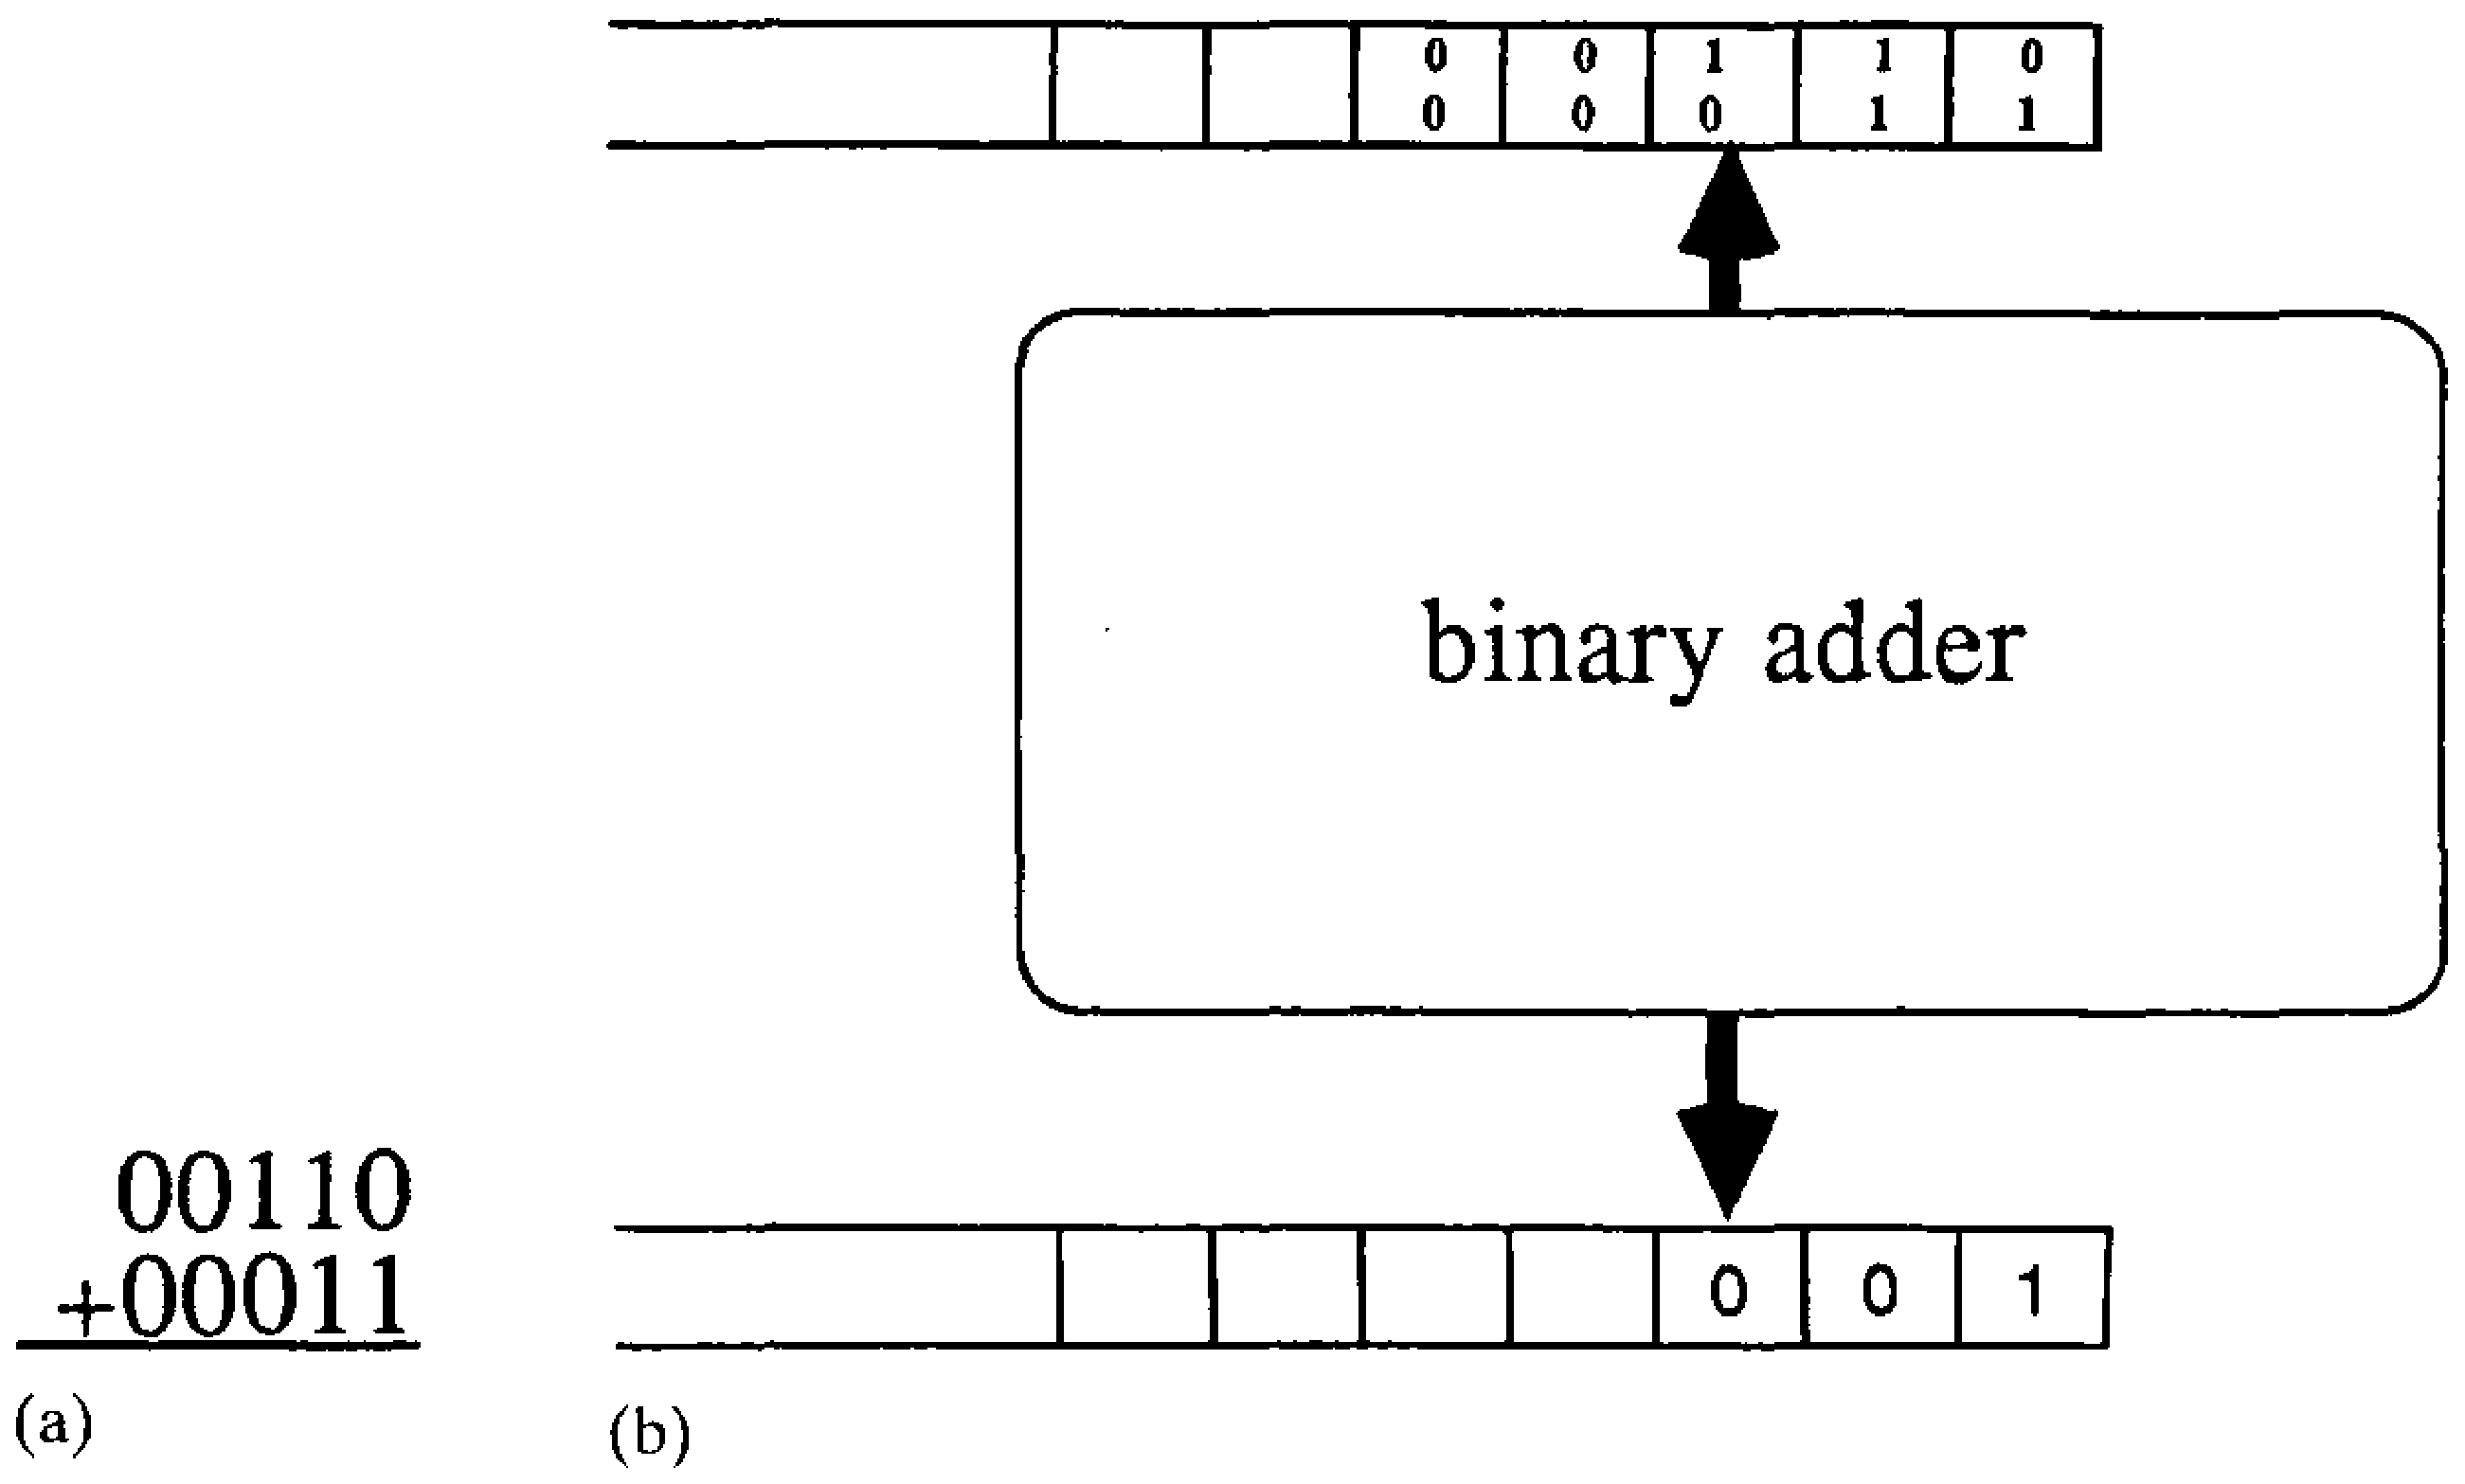
\epsfig{figure=ToFAfigures/fig7-11.eps,width=5.5in}}
\caption{(a) The addition problem discussed in Example 7.15 (b) Conceptual model
of the binary adder discussed in Example 7.15}\label{fig-7.11}
\end{figure}

% Figure 7.12
\begin{figure}
\centerline{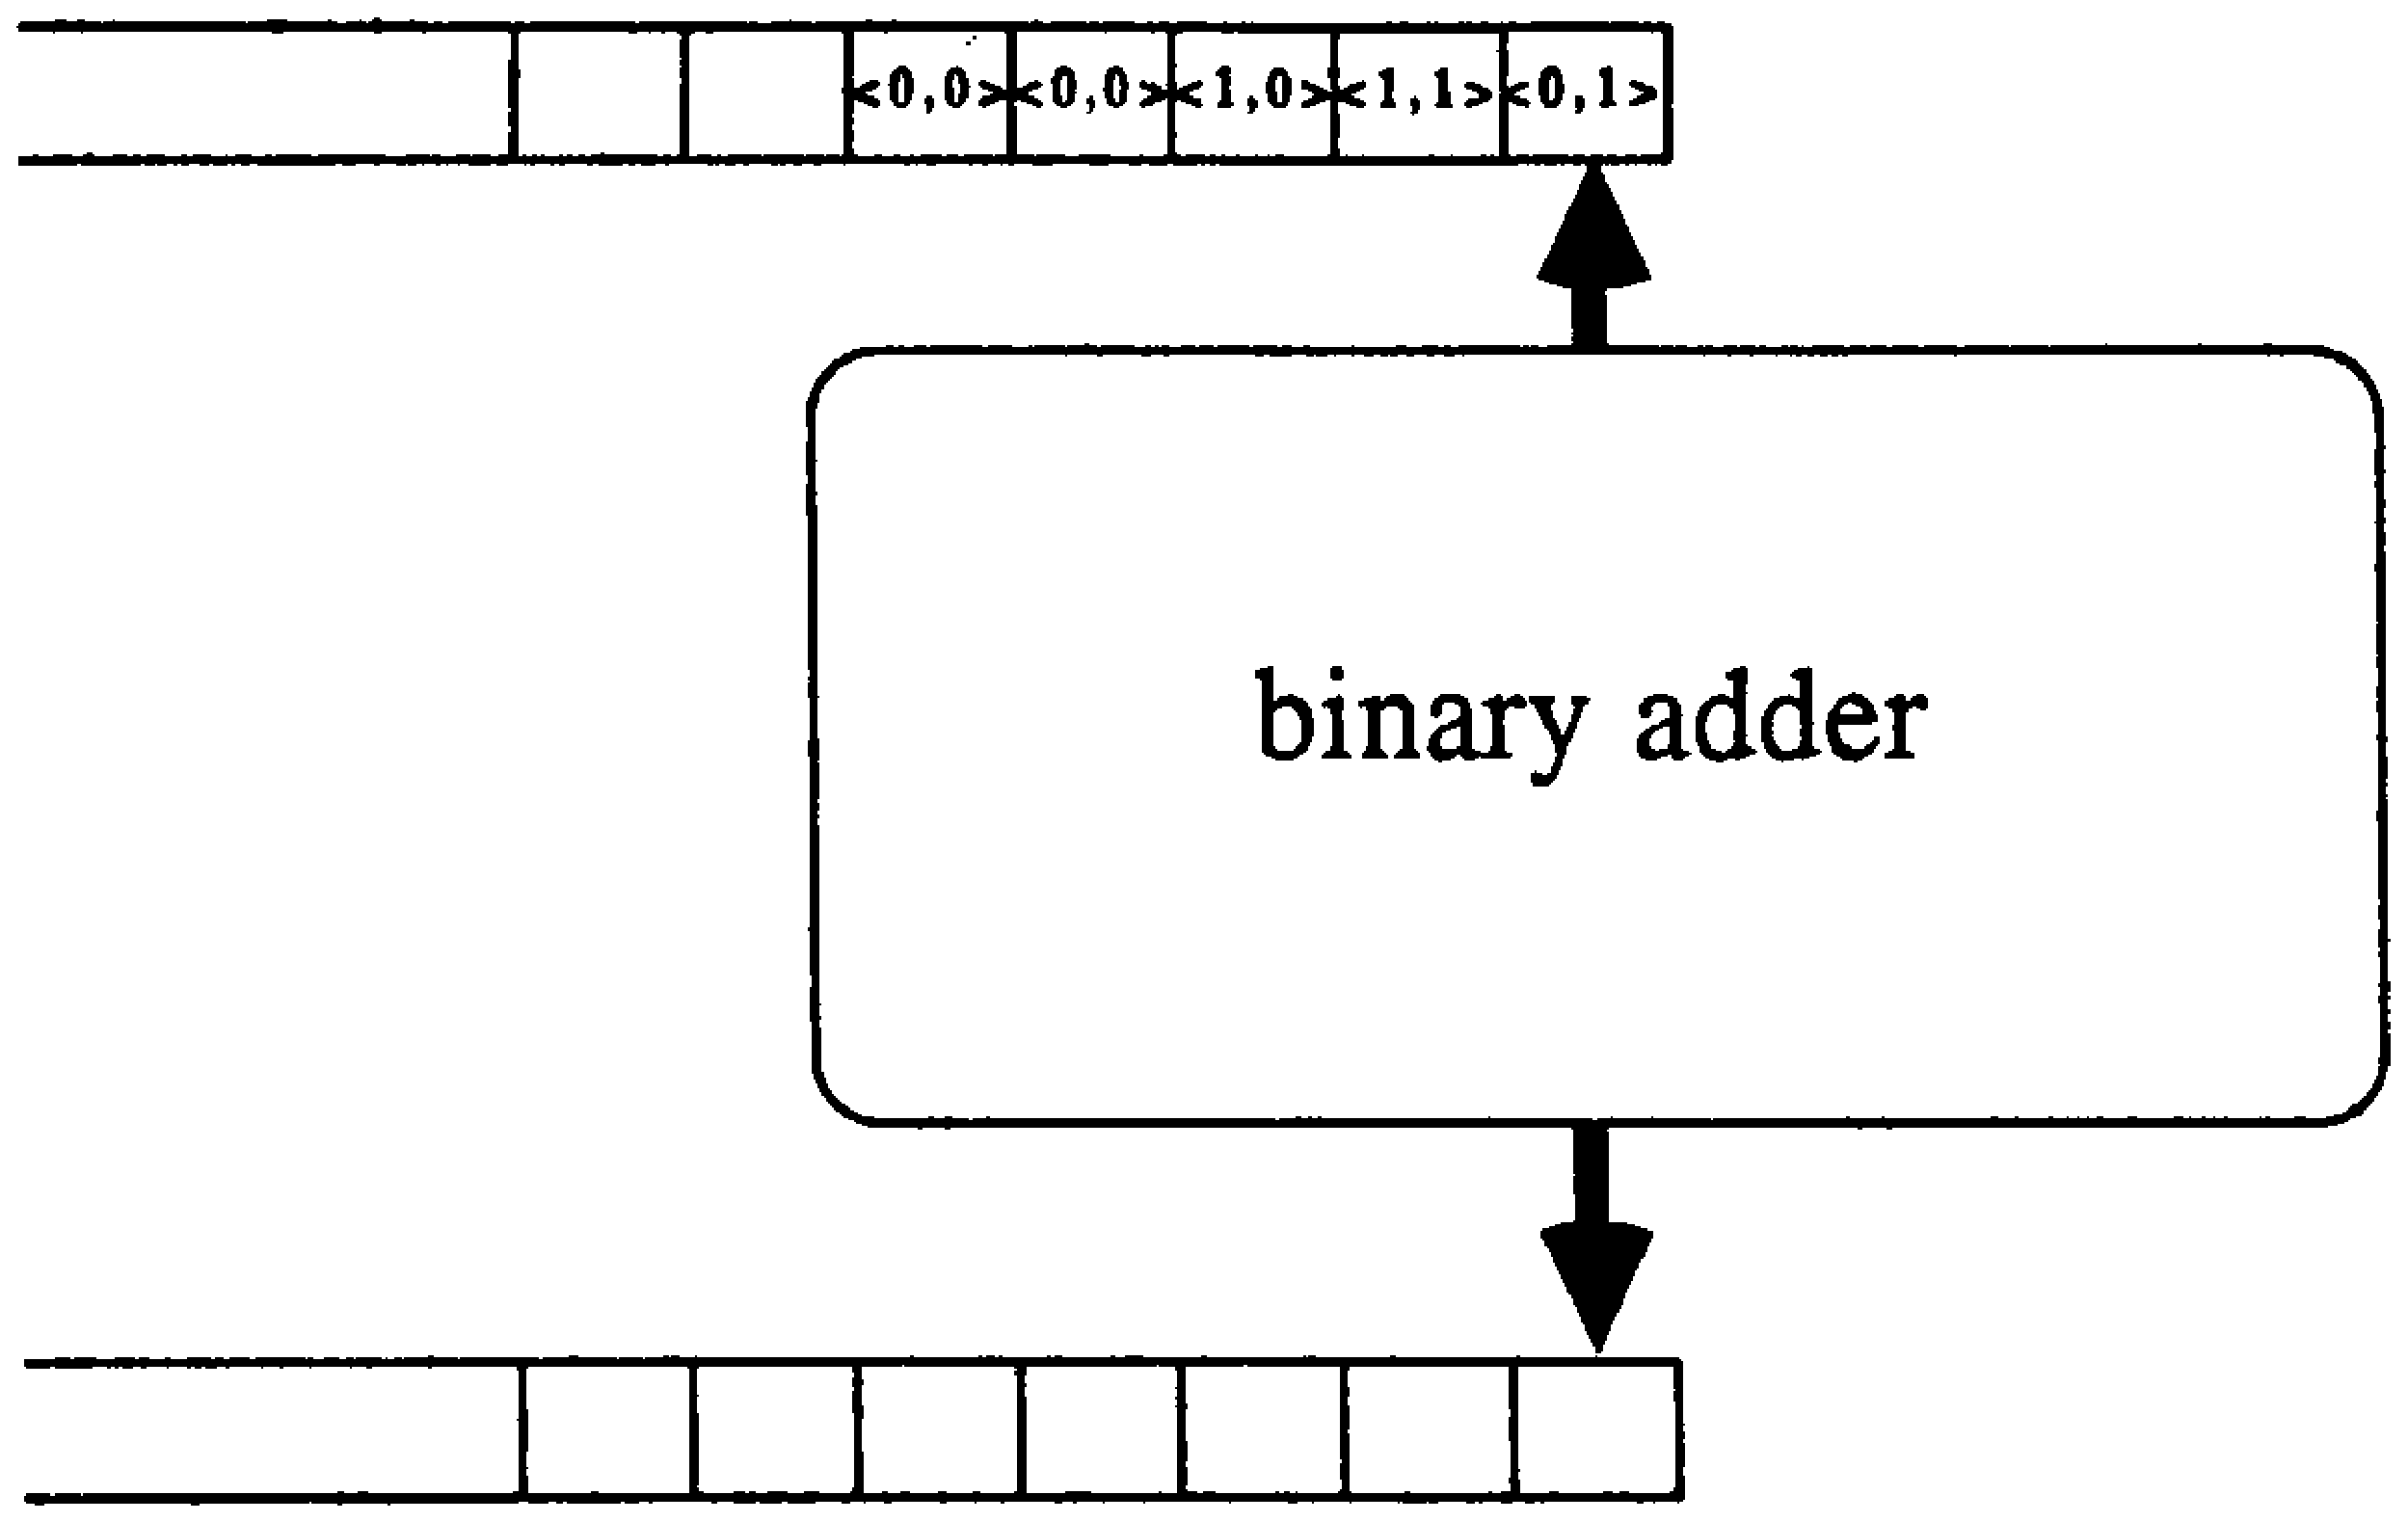
\epsfig{figure=ToFAfigures/fig7-12.eps,width=5.5in}}
\caption{The binary adder discussed in Example 7.15}\label{fig-7.12}
\end{figure}

Unfortunately, addition is not truly length preserving; adding the three-digit
numbers $\pmb{110}$ and $\pmb{011}$ produces a binary answer that is four digits
long. The adder $B$ defined in Example 7.15 cannot correctly reflect a carry out
of the most significant binary position. While the concept of final states is
not present in our formal definition of transducers, this FST $B$ provides an
example in which it is natural to both produce continuous output and track the
terminal state: if a computation ends in state $C$, then we know that an
overflow condition has occurred. $B$ clearly operates correctly on all strings
that have been padded with $\langle 0,0\rangle$ as the last (leftmost) symbol;
employing such padding is reminiscent of the use of the \<EOS\> symbol when
building circuits for DFAs. Indeed, it might be profitable to specifically
include an \<EOS\> symbol and have the transducer react to \<EOS\> by printing a
$\pmb{y}$ or $\pmb{n}$ to indicate whether or not there was overflow.

% Figure 7.13
\begin{figure}
\centerline{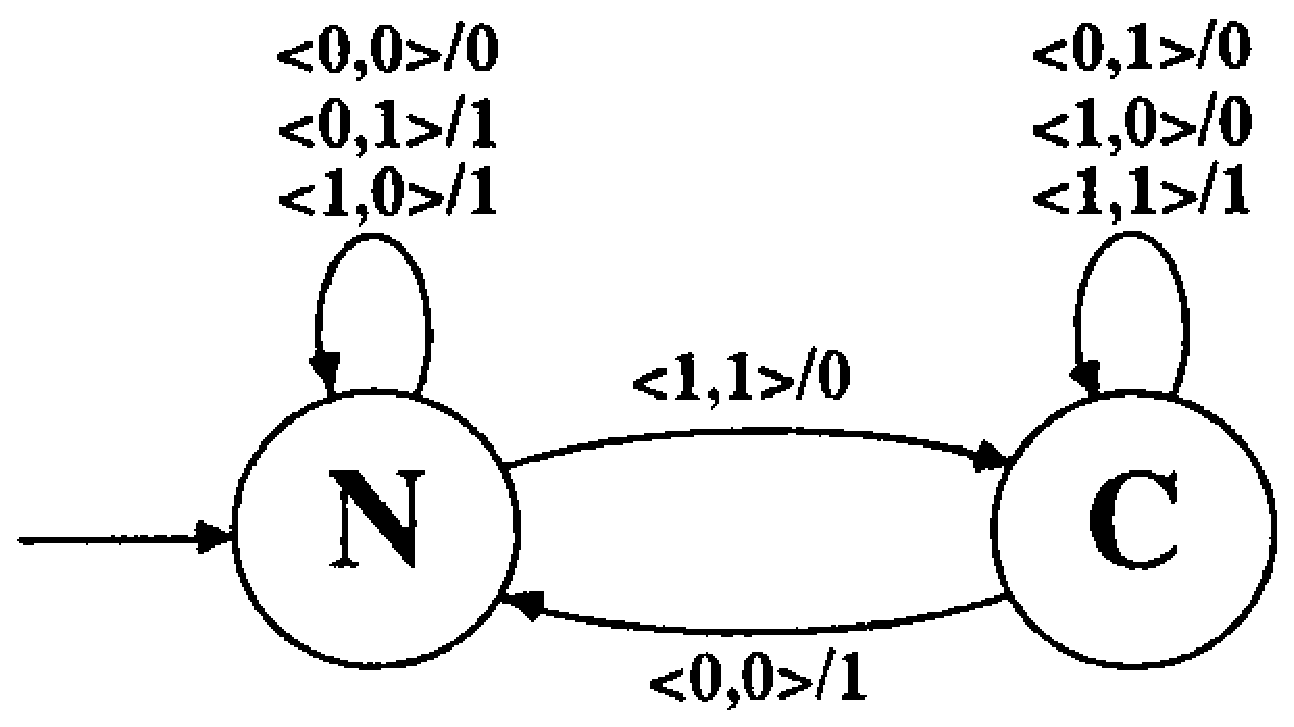
\epsfig{figure=ToFAfigures/fig7-13.eps,width=2.5in}}
\caption{The state transition diagram for a binary adder modeled as a Mealy
machine, as discussed in Example 7.15}\label{fig-7.13}
\end{figure}

While the binary adder is only one small component of a computer, finite-state
transducers can be profitably used to model complete systems; one such
application involves traffic lights. The controller for a large intersection
may handle eight banks of traffic signals for the various straight-ahead and
left-turn lanes, as well as four sets of walk lights (see the exercises). Input
about the intersection conditions is often fed to the controller from pedestrian
walk buttons and metal detectors embedded in the roadway. For simplicity, we
will choose a simplified intersection to illustrate how to model a traffic
controller by a transducer. The simplified example nevertheless incorporates all
the essential features of the more intricate intersections. A full-blown model
would only require larger alphabets and more states.

\subsection*{Example 7.16}

Consider a small north-south street that terminates as it meets a large
east-west avenue, as shown in Figure \ref{fig-7.14}. Due to the heavy traffic along the
avenue, the westbound traffic attempting to turn left is governed by a left-turn
signal (signal 2 in Figure \ref{fig-7.14}). Traffic continuing west is controlled by
signal 1, while signal 3 governs eastbound traffic. Vehicles entering the
intersection from the south rely on signal 4. The red, yellow, and green lights
of these four signals represent the output of the transducer. Protecting
westbound traffic while turning left is accomplished by an output configuration
of $\langle G,G,R,R\rangle$, which is meant to indicate that the first two
signals are green while the eastbound and northbound lanes have red lights. The
output alphabet can thus be represented by ordered foursomes of $R,\ Y$, and $G$
(red, yellow, and green). We can succinctly define
\[ \Gamma=\{R,Y,G\} \times \{R,Y,G\} \times \{R,Y,G\} \times \{R,Y,G\}, \]
though there will be some combinations (like $\langle G,G,G,G\rangle$) that are
not expected to appear in the model.

% Figure 7.14
\begin{figure}
\centerline{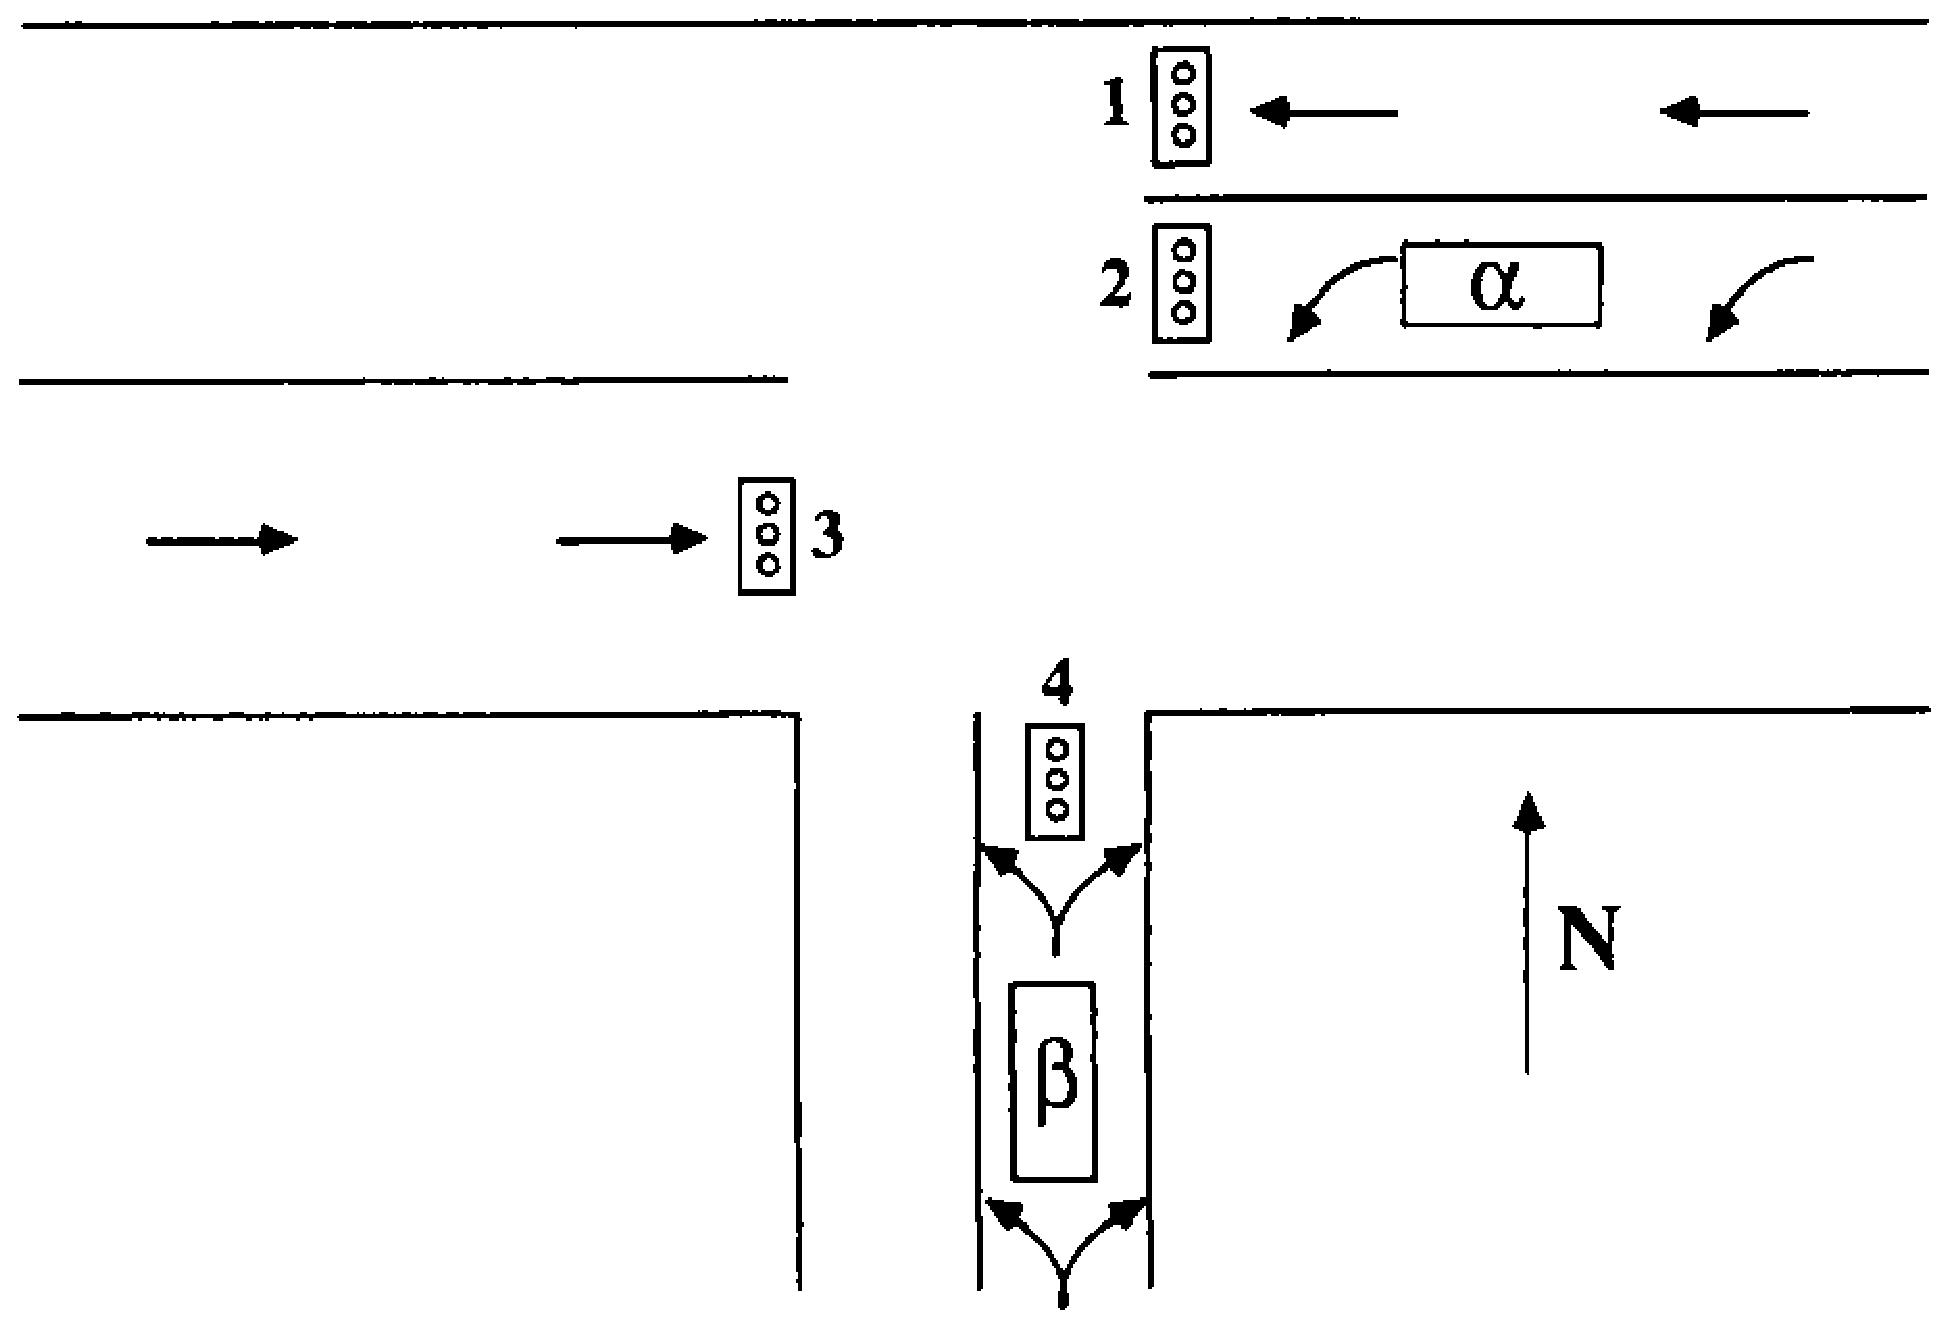
\epsfig{figure=ToFAfigures/fig7-14.eps,width=3.5in}}
\caption{The intersection discussed in Example 7.16}\label{fig-7.14}
\end{figure}

The most prevalent output configuration is expected to be $\langle
G,R,G,R\rangle$, which allows unrestricted flow of the east-west traffic on the
avenue. Due to the relatively small amount of traffic on the north-south street,
the designers of the intersection chose to embed the sensors $\alpha$ in the
left-turn lane and $\beta$ in the northbound lane and only depart from the
$\langle G,R,G,R\rangle$ configuration when a vehicle is sensed by these
detectors. There is therefore a pair of inputs to our transducer, indicating the
status of sensor $\alpha$ and sensor $\beta$. The four combinations will be
represented by $\langle 0,0\rangle$, (no traffic above either sensor), $\langle
1,0\rangle$ (sensor $\alpha$ active), $\langle 0,1\rangle$ (sensor $\beta$
active), and $\langle 1,1\rangle$ (both detectors have currently sensed
vehicles).

The controller is most naturally modeled by a Moore machine, since the state
of the system is so intimately tied to the status of the four lights. From the
configuration $\langle G,R,G,R\rangle$, activation of the $\beta$ sensor
signifies that all traffic should be stopped except that governed by signal 4.
The output should therefore move through the pattern $\langle Y,R,Y,R\rangle$ to
$\langle R,R,R,G\rangle$ and remain in that state until the $\beta$ sensor is
deactivated. This and the other transitions are illustrated in Figure \ref{fig-7.15}.

% Figure 7.15
\begin{figure}
\centerline{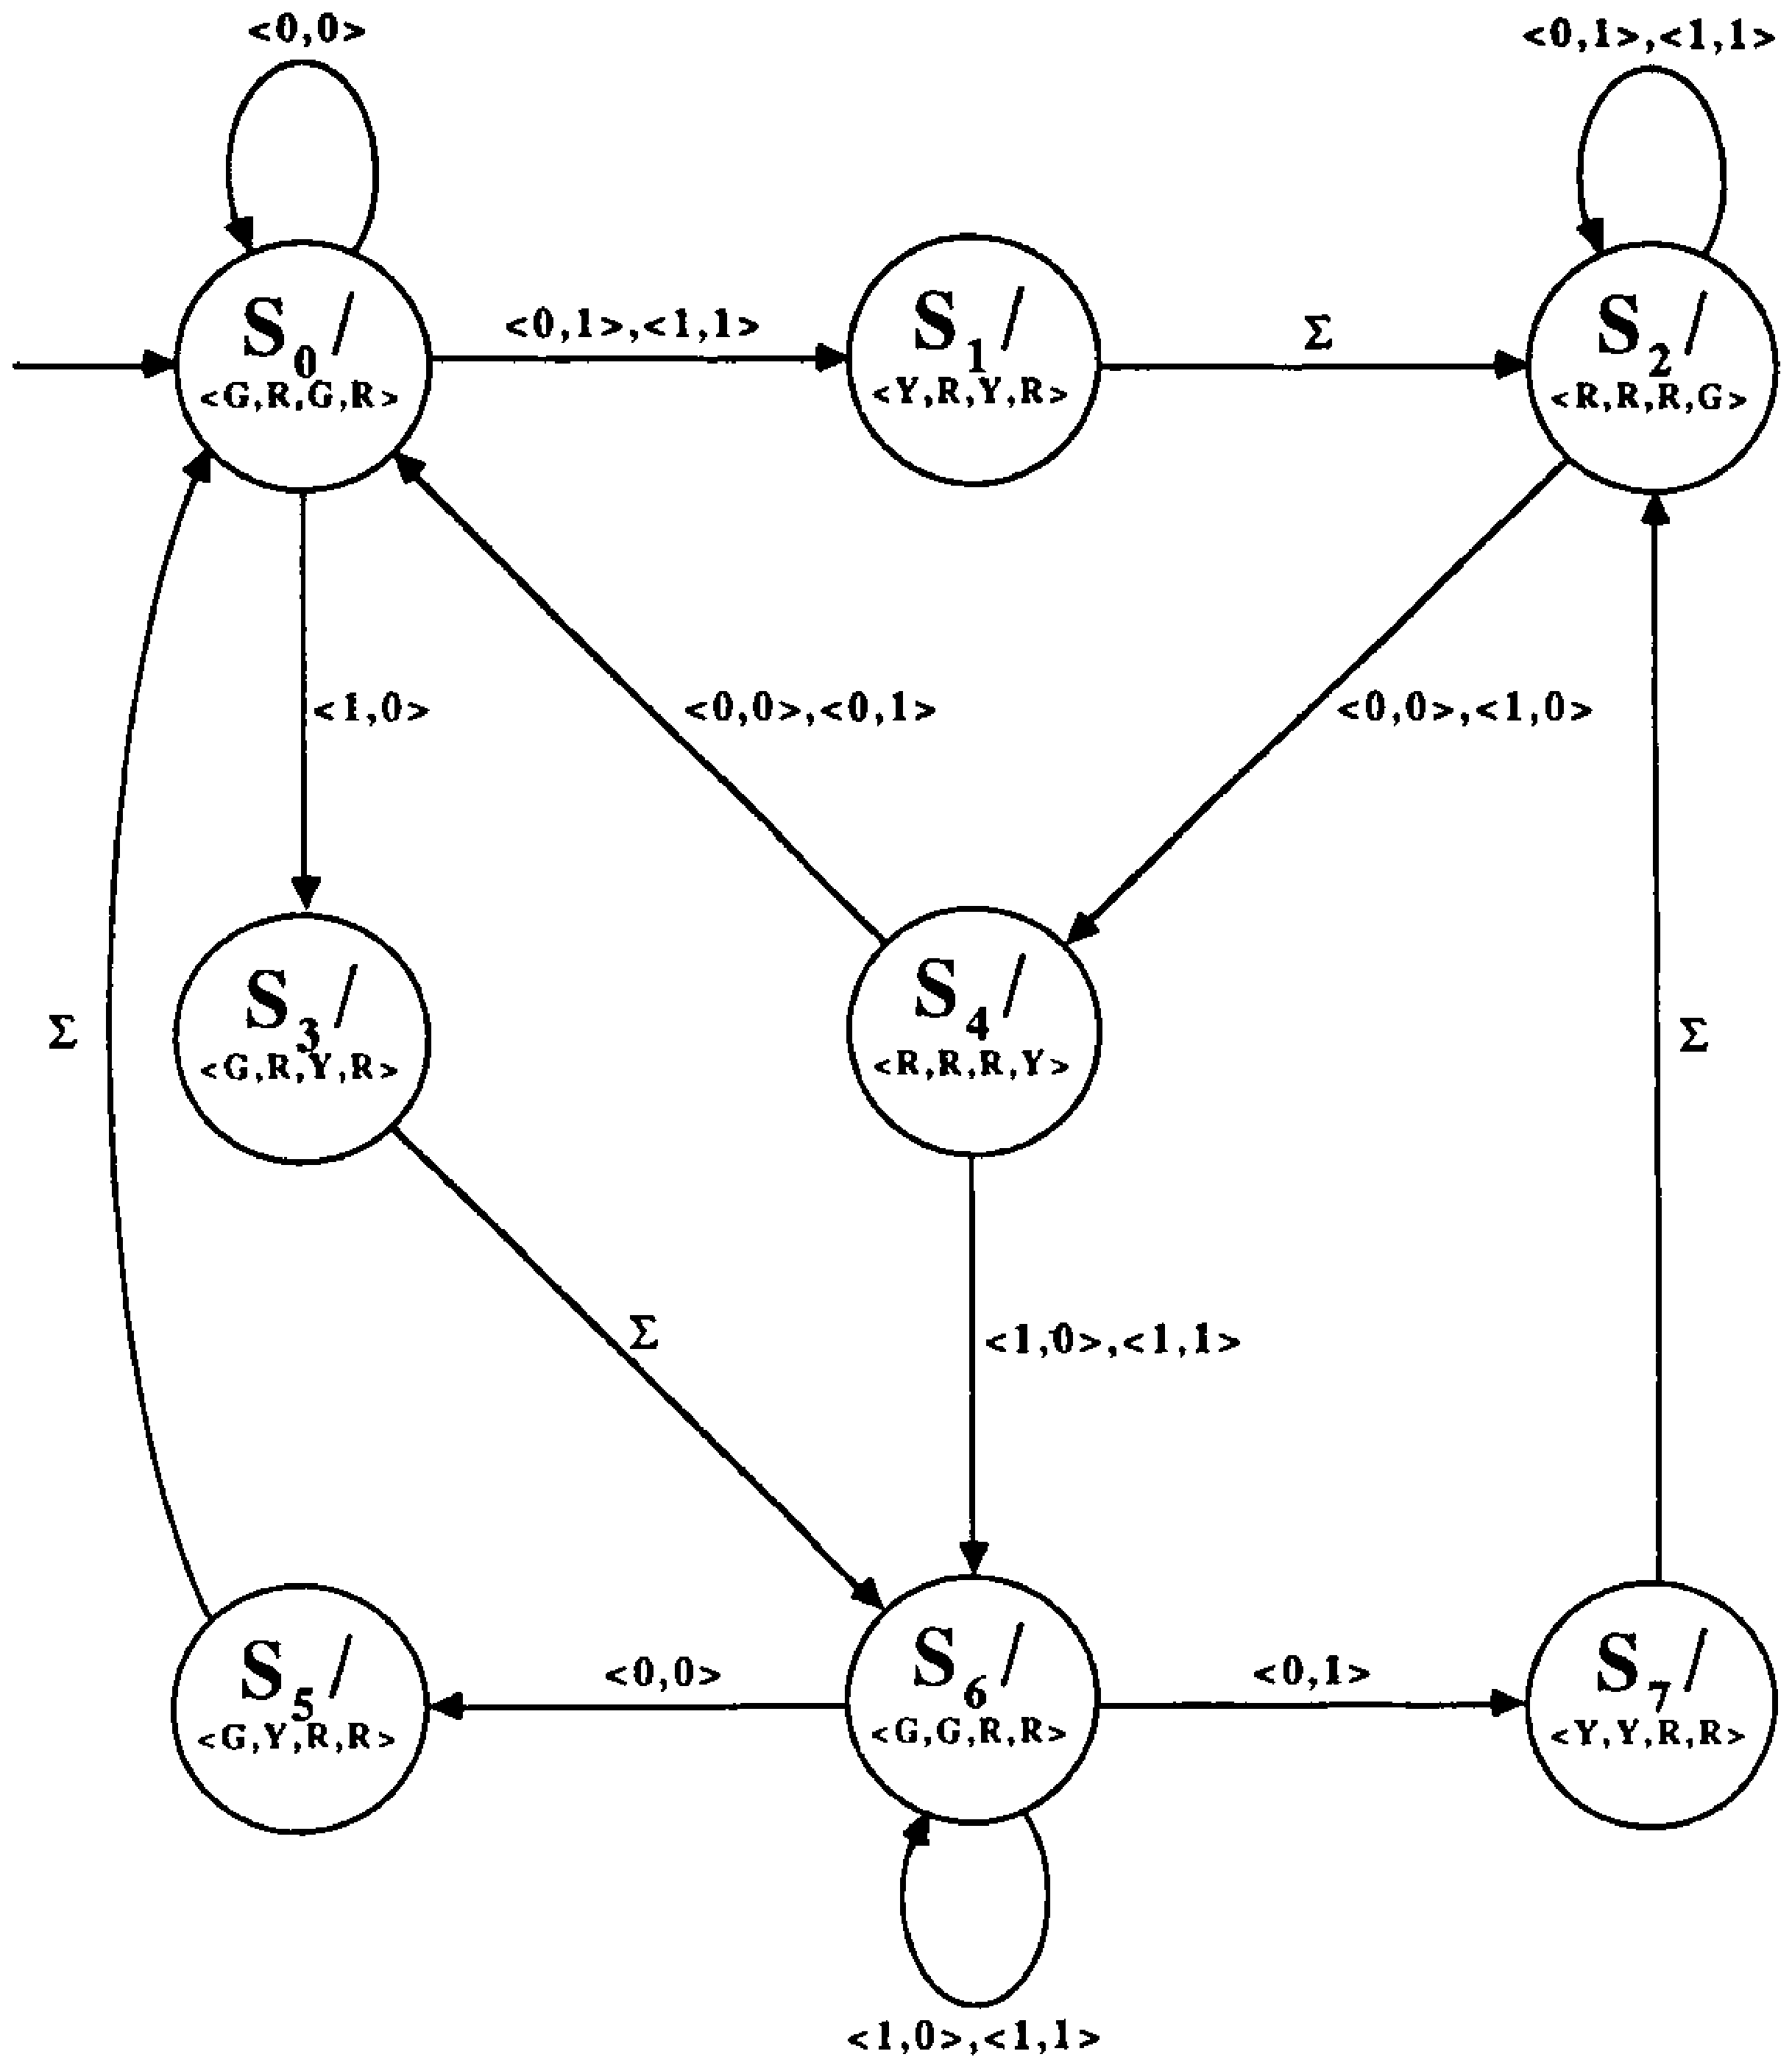
\epsfig{figure=ToFAfigures/fig7-15.eps,width=3.5in}}
\caption{The state transition diagram for a stoplight modeled as a
Moore machine, as discussed in Example 7.16}\label{fig-7.15}
\end{figure}

In actuality, the duration of patterns incorporating the yellow caution light
is shorter than others. With the addition of extra states, a clock cycle length
on the order of 5 seconds (commensurate with the typical length of a yellow
light) could be used to govern the length of the different output configurations.
For example, incorporating $s_g$ as shown in Figure \ref{fig-7.16} guarantees that the
output $\langle R,R,R,G\rangle$ will persist for at least two cycles (10
seconds). From an engineering standpoint, complicating the finite-state control
in this manner can be avoided by varying the clock cycle length.

% Figure 7.16
\begin{figure}
\centerline{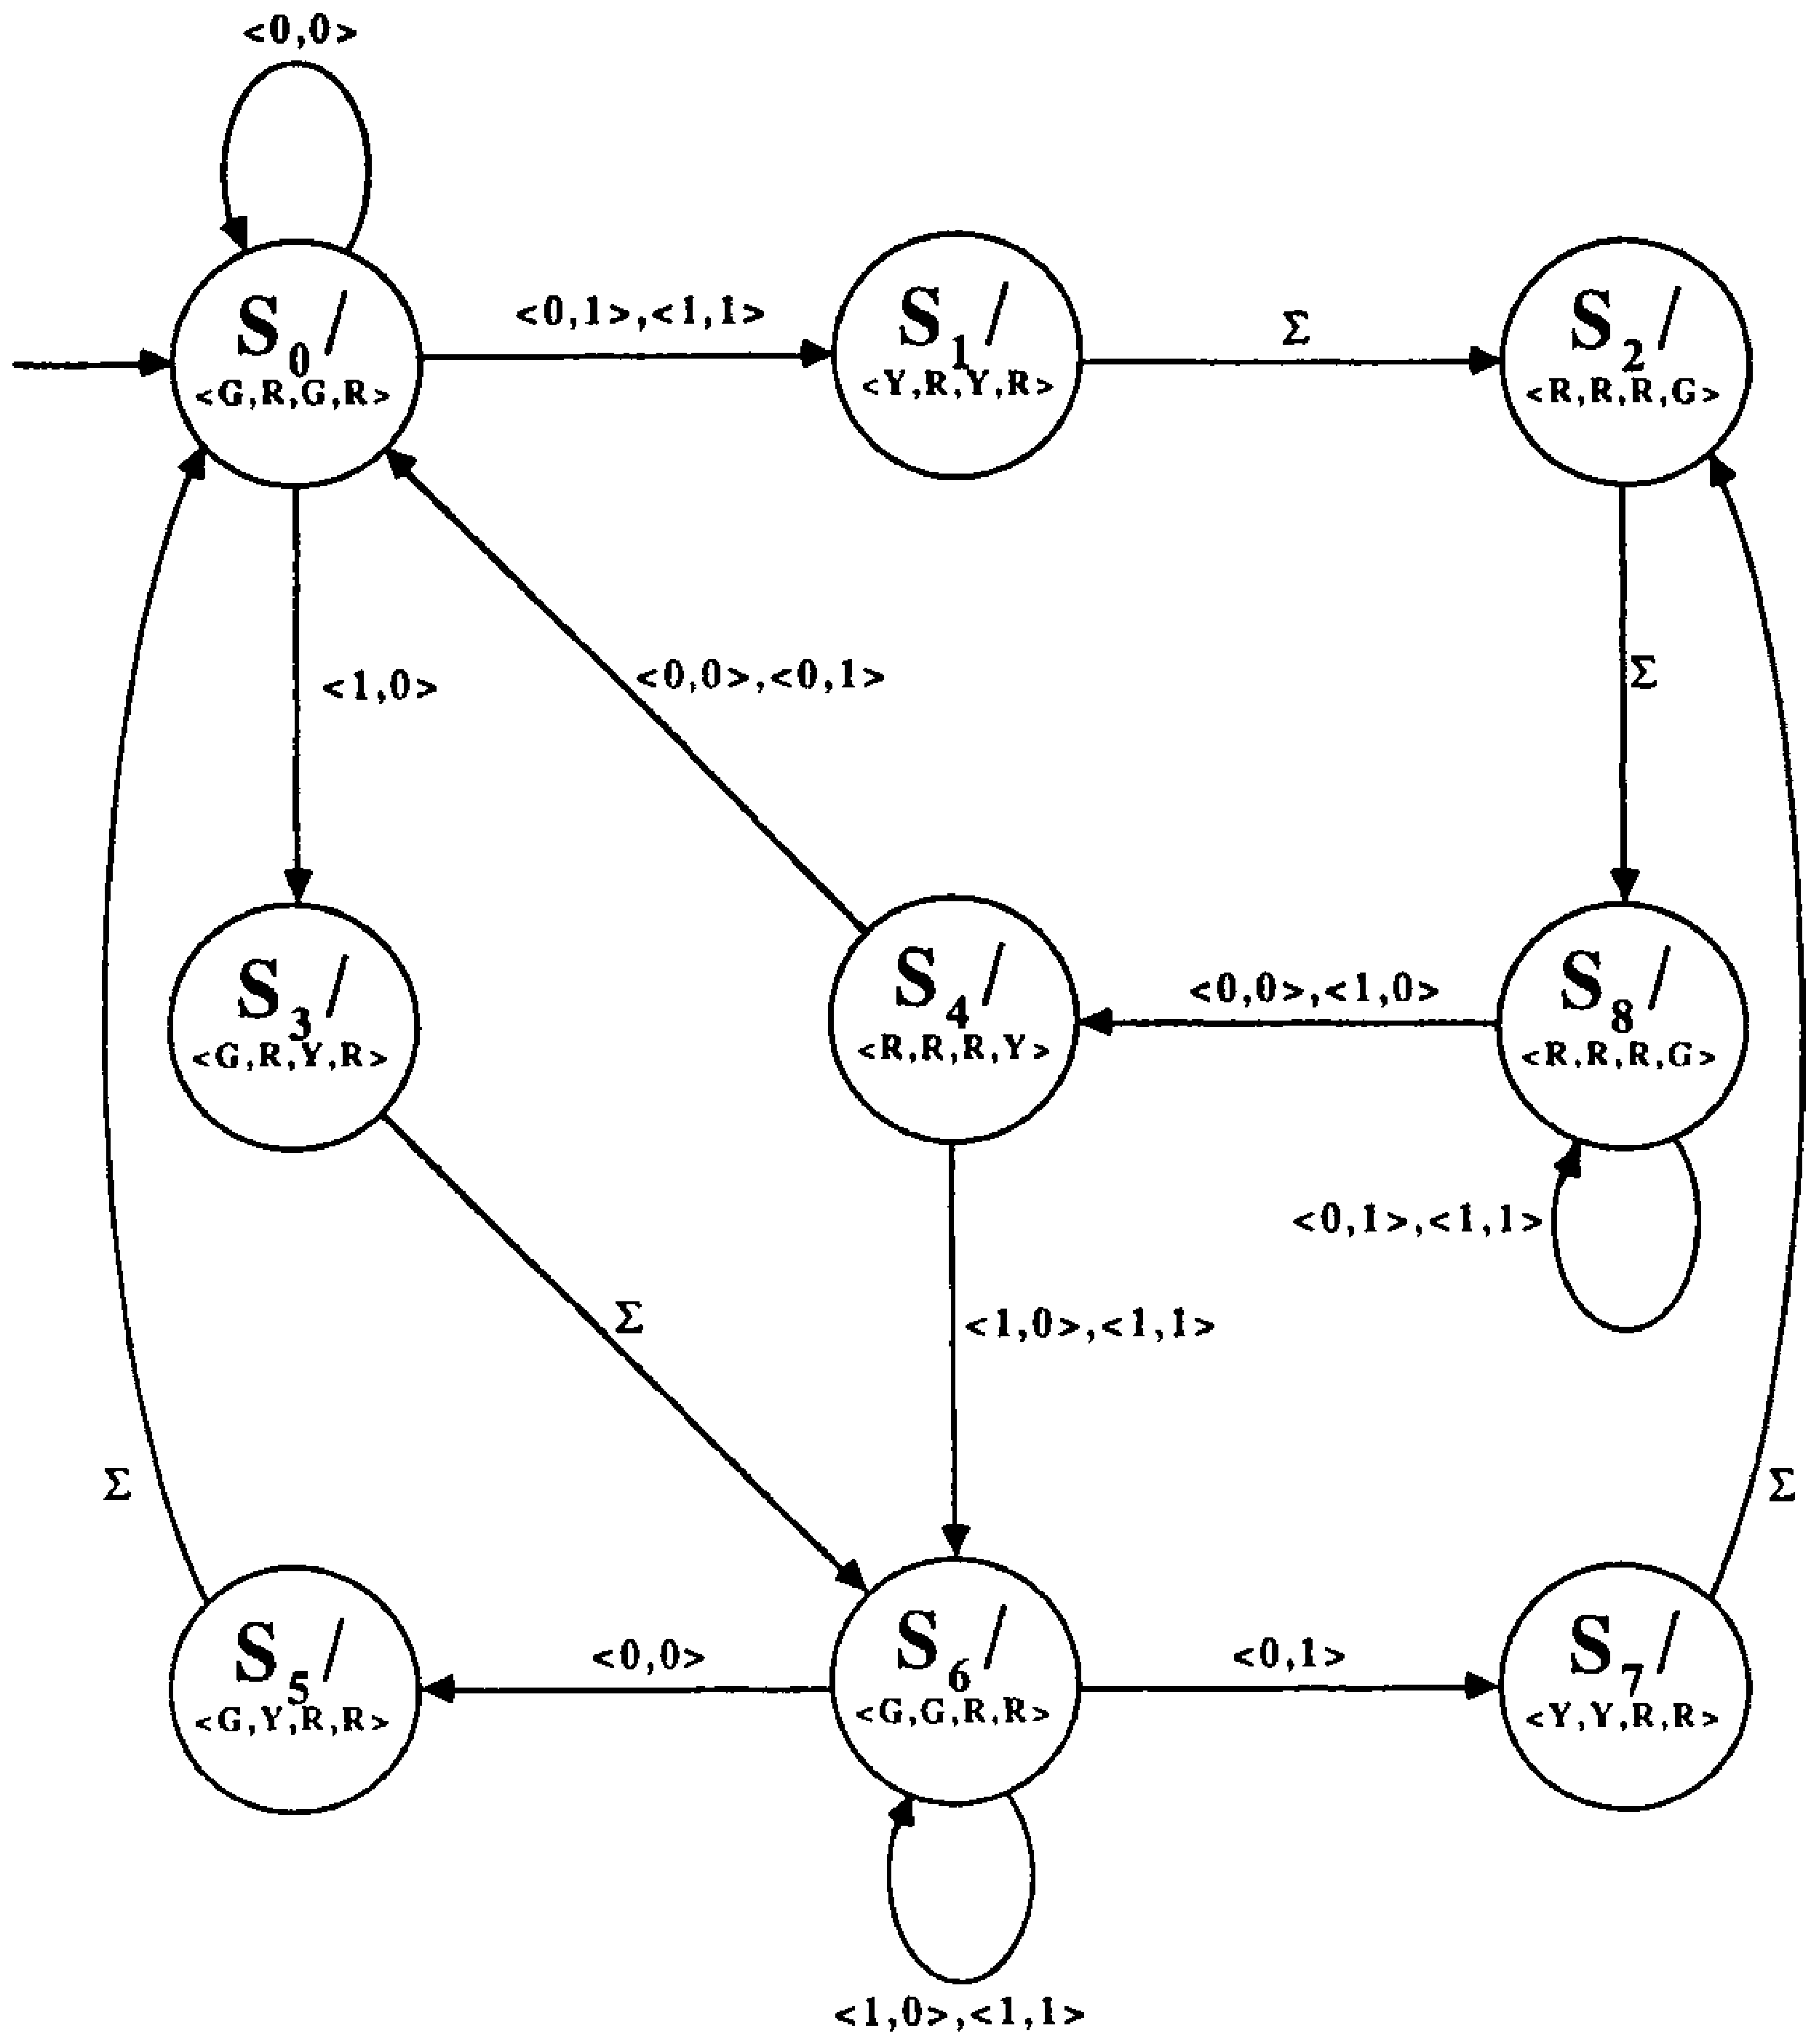
\epsfig{figure=ToFAfigures/fig7-16.eps,width=3.0in}}
\caption{The modified controller discussed in Example 7.16}\label{fig-7.16}
\end{figure}

We now discuss some of the hardware that comprise the heart of traffic
controllers and vending machines. As was done with deterministic finite
automata in Chapter \ref{ch-1} and nondeterministic finite automata in Chapter \ref{ch-4},
finite-state transducers can be implemented with digital logic circuits. We
again use a clock pulse, D flip-flops, and an encoding for the states. Besides
needing an encoding for the input alphabet, it is now necessary to have an
encoding for the output alphabet, which will be represented by the bits
$w_1,w_2,w_3,\ldots$. We again suggest (solely for simplicity and
standardization in the exercises) ordering the symbols in $\Gamma$
alphabetically and assigning binary codes in ascending order, as was recommended
earlier for $\Sigma$. We must construct a circuit for generating each $w_j$, in
the same manner as we built circuits implementing the accept function for finite
automata.

Many practical applications of FSTs (such as traffic signals) operate
continuously, rather than starting and stopping for one small string. In such
cases, an \<EOS\> symbol is not necessary; the circuit operates until power is
shut off. Similarly, an \<SOS\> symbol is not essential for a traffic signal
complex; upon resuming operation after a power failure, it is usually immaterial
whether east-west traffic first gets a green light or whether it gets a red
light in deference to the north-south traffic. In contrast, it is important for
vending machines to initialize to the proper state or some interesting discounts
could be obtained by playing with the power cord.

\subsection*{Example 7.17}

Consider the FST displayed in Figure \ref{fig-7.17}. If \<EOS\> and \<SOS\> is
unnecessary, then the input alphabet can be represented by a single bit $a_1$,
with $a_1=\pmb{0}$ representing $\pmb{c}$ and $a_1=\pmb{1}$ representing $\pmb{d}$.
Similarly, the output alphabet can be represented by a single bit $w_1$ with
$w_1=\pmb{0}$ representing $\pmb{a}$ and $w_1=\pmb{1}$ representing $\pmb{b}$. The
states can likewise be represented by a single bit $t_1$, with $t_1=\pmb{0}$
representing $s_0$ and $t_1=\pmb{1}$ representing $s_1$. As before, we can
construct a truth table to represent the state transition function, defining
$t'_1$ in terms of $t_1$ and $a_1$. The complete table is given in Table 7.5a.

% Figure 7.17
\begin{figure}
\centerline{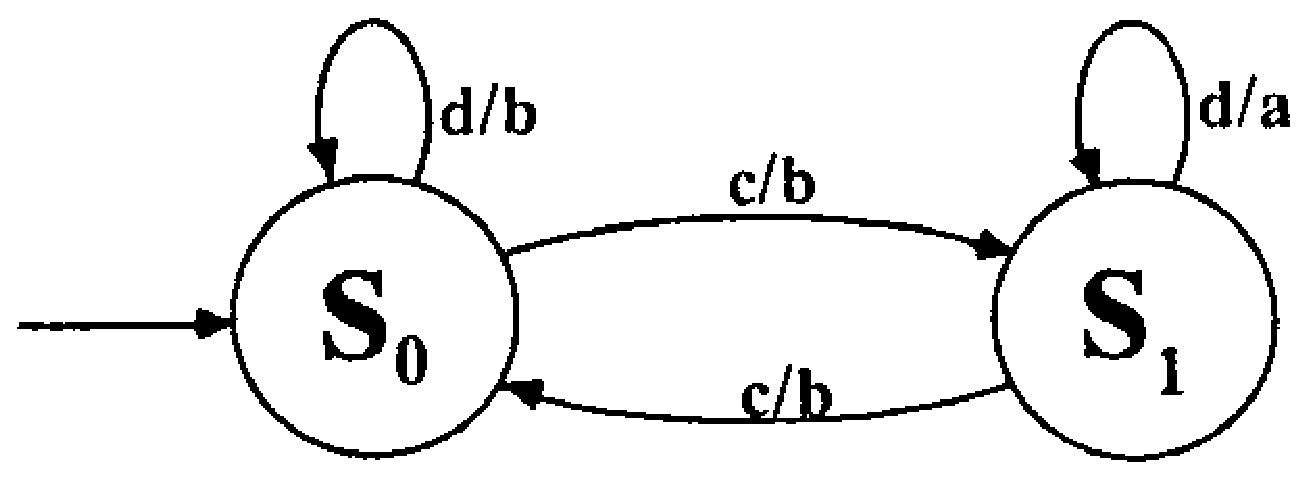
\epsfig{figure=ToFAfigures/fig7-17.eps,width=2.5in}}
\caption{The state transition diagram for the Mealy machine in Example 7.17}\label{fig-7.17}
\end{figure}

% Table 7.5a & 7.5b
\begin{table}\label{tbl-7.5}
\begin{center}
\begin{tabular}{cc|c}
\multicolumn{3}{c}{Table 7.5a} \\
$t_1$ & $a_1$ & $t'_1$ \\
\hline
$\pmb{1}$ & $\pmb{1}$ & $\pmb{1}$ \\
$\pmb{0}$ & $\pmb{1}$ & $\pmb{0}$ \\
$\pmb{1}$ & $\pmb{0}$ & $\pmb{0}$ \\
$\pmb{0}$ & $\pmb{0}$ & $\pmb{1}$
\end{tabular}
$\qquad$
\begin{tabular}{cc|c}
\multicolumn{3}{c}{Table 7.5b} \\
$t_1$ & $a_1$ & $w_1$ \\
\hline
$\pmb{1}$ & $\pmb{1}$ & $\pmb{0}$ \\
$\pmb{0}$ & $\pmb{1}$ & $\pmb{1}$ \\
$\pmb{1}$ & $\pmb{0}$ & $\pmb{1}$ \\
$\pmb{0}$ & $\pmb{0}$ & $\pmb{1}$
\end{tabular}
\end{center}
\end{table}

% Figure 7.18
\begin{figure}
\centerline{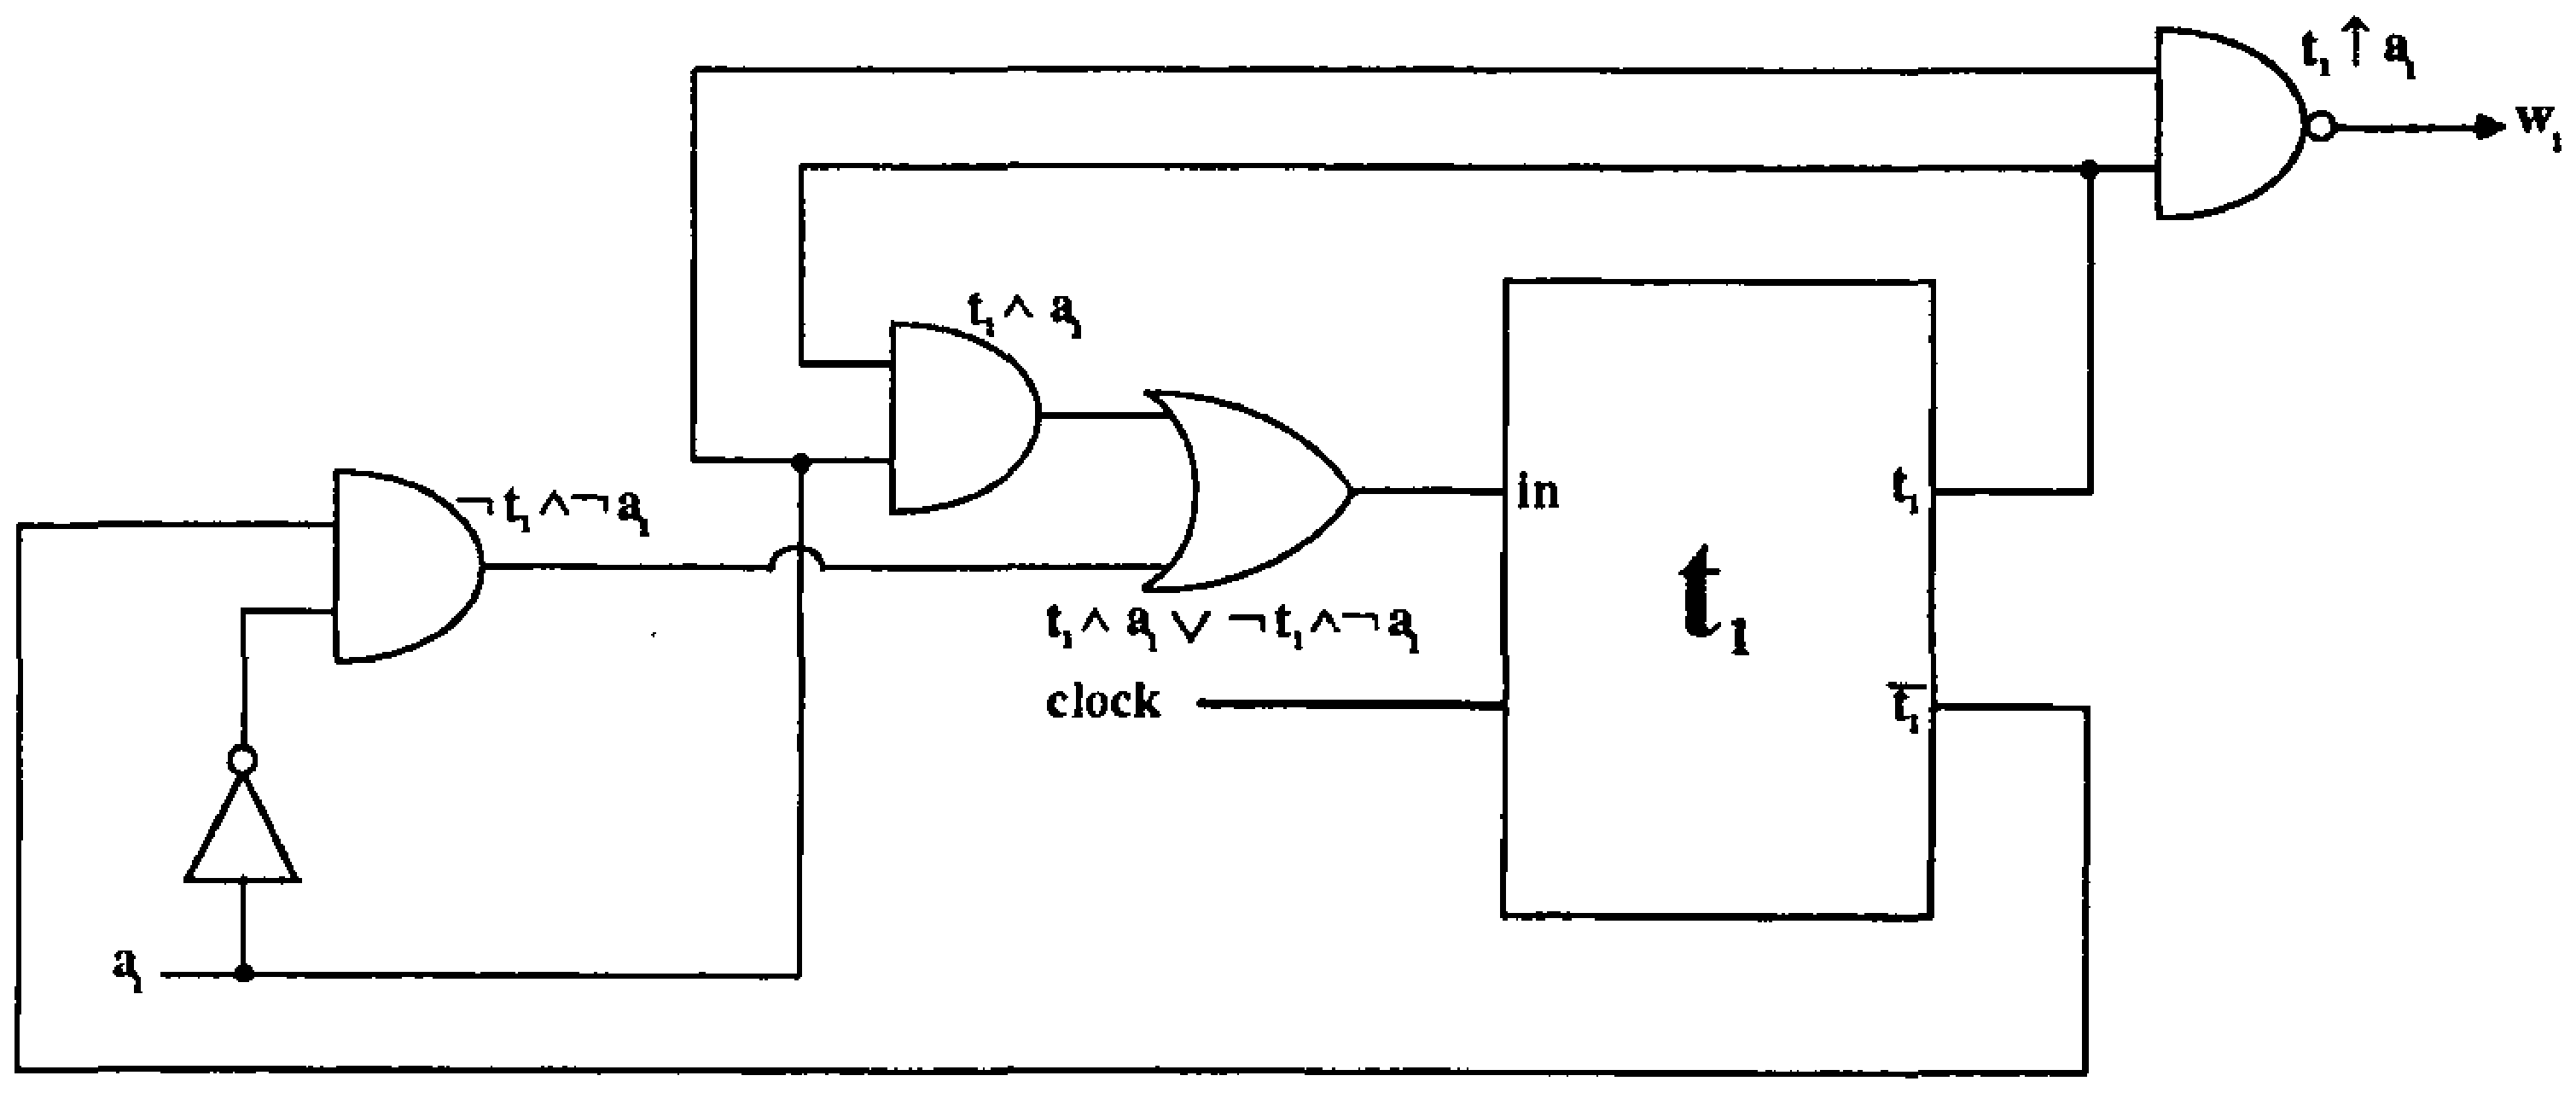
\epsfig{figure=ToFAfigures/fig7-18.eps,width=4.5in}}
\caption{Circuit diagram for Example 7.17}\label{fig-7.18}
\end{figure}

The principal disjunctive normal form for the transition function is therefore
seen to be $t'_1=(t_1 \wedge a_1)\vee(\neg t_1 \wedge \neg a_1)$. The output
function can be found in a similar manner, as shown in Table 7.5b.

Thus, $w_1=(t_1 \uparrow a_1)$. As in Example 1.12, the circuit for $t_1$, will
be fed back into the D flip-flop(s); the circuit for $w_1$ will form the output
for the machine (replacing the acceptance circuit used in DFAs). The complete
network is shown in Figure \ref{fig-7.18}. Note that we would want the output device to
print on the rising edge of the clock cycle, before the new value of $t_1$
propagates through the circuitry.

A larger output alphabet would require an encoding of several bits; each $w_1$
would have its own network of gates, and the complete circuit would then
simultaneously generate several bits of output information. As in Chapter \ref{ch-1},
additional states or input symbols will add bits to the other encoding schemes
and add to the number of rows in the truth tables for $\delta$ and $\omega$.
Each additional state bit will also require its own D flip-flop and a new truth
table for its feedback loop. Each additional state bit doubles the number of
states that can be represented, which means that, as was the case with
deterministic finite automata, the number of flip-flops grows as the logarithm
of the number of states.

\section*{Exercises}
\begin{enumerate}[{7.}1.]
\item Let $A=\langle\Sigma,\Gamma,S,s_0,\delta,\omega\rangle$ be a Mealy
machine. Prove the following statements from Theorem \ref{thm-7.1}:
\begin{enumerate}
\item $(\forall x \in \Sigma^*)(\forall y \in \Sigma^*)(\forall t \in S)
	(\OBAR(t,yx) = \OBAR(t,y) \cdot \OBAR(\DBAR(t,y),x))$
\item $(\forall x \in \Sigma^*)(\forall y \in \Sigma^*)(\forall s \in S)
	(\DBAR(s,yx) = \DBAR(\DBAR(s,y),x))$
\end{enumerate}

\item Refer to Lemma \ref{lmm-7.1} and prove:
\begin{enumerate}
\item $(\forall s \in S_A)(\forall x \in \Sigma^*)(\mu(\DBAR_A(s,x)) =
	\DBAR_B(\mu(s),x))$
\item $(\forall s \in S_A)(\forall x \in \Sigma^*)(\OBAR_A(s,x) =
	\OBAR_B(\mu(s),x))$
\end{enumerate}

\item Prove Corollary \ref{cor-7.3}.

\item Prove Corollary \ref{cor-7.4} by showing that a necessary and sufficient condition
for a Mealy machine $M$ to be minimal is that $M$ is both reduced and connected.

\item Show that any FTD function $f$ must satisfy a ``pumping lemma.''
\begin{enumerate}
\item Devise the statement of a theorem that shows that the way any sufficiently
long string is translated determines how an entire sequence of longer strings
are translated.
\item Prove the statement made in part (a).
\end{enumerate}

\item In each of the following parts, you may assume the results in the
preceding parts; for example, you may assume parts (a) and (b) when proving (c).
\begin{enumerate}
\item Prove Lemma \ref{lmm-7.3}a.
\item Prove Lemma \ref{lmm-7.3}b.
\item Prove Lemma \ref{lmm-7.3}c.
\item Prove Lemma \ref{lmm-7.3}d.
\item Prove Lemma \ref{lmm-7.3}e.
\end{enumerate}

\item Given a FST $M=\langle\Sigma,\Gamma,S,s_0,\delta,\omega\rangle$, prove the
following statements from Lemma \ref{lmm-7.4}:
\begin{enumerate}
\item $E_{0M}$ has just one equivalence classes, which consists of all of $S$.
\item $E_{1M}$ is defined by $s E_{1M} t \Leftrightarrow (\forall \pmb{a} \in \Sigma)
	(\omega(s,\pmb{a}) = \omega(t,\pmb{a}))$.
\item $(\forall s \in S)(\forall t \in S)(\forall i \geq 1)(s E_{i+1M} t
	\Leftrightarrow s E_{iM} t \wedge (\forall\pmb{a}\in\Sigma)
	(\delta(s,\pmb{a}) E_{iM} \delta(t,\pmb{a}))$.
\end{enumerate}

\item Prove Theorem \ref{thm-7.6} by showing that if $A=\langle\Sigma,\Gamma,S,s_0,\delta,
\omega\rangle$ is a Moore machine then \[(\forall x \in \Sigma^*)(\forall y \in
\Sigma^*)(\forall t \in S)(\OBAR(t,yx) = \OBAR(t,y) \cdot \OBAR(\DBAR(t,y),x))\]

\item Prove Theorem \ref{thm-7.7}.

\item Prove Theorem \ref{thm-7.8}.

\item Use Lemma \ref{lmm-7.6} to find $E_C$ in Example 7.10.

\item Show that there is a homomorphism from the machine $M$ in Example 7.11 to
the machine $B$ in Example 7.2.

\item Prove that, in a FST $M=\langle\Sigma,\Gamma,S,s_0,\delta,\omega\rangle,\ 
(\forall t \in S)(\forall\pmb{a}\in\Sigma)(\OBAR(t,\pmb{a})=\omega(t,\pmb{a}))$.

\item Modify the vending machine in Example 7.1 so that it can return all the
coins that have been inserted. Let $\pmb{r}$ denote a new input that represents
activating the coin return, and let $\pmb{a}$ represent a new output corresponding
to the vending machine releasing all the coins in its temporary holding area.

\item Given a FST $M=\langle\Sigma,\Gamma,S,s_0,\delta,\omega\rangle$ and
$M/\!\!_{E_M}=\langle\Sigma,\Gamma,S_{E_M},s_{0_{E_M}},\delta_{E_M},\omega_{E_M}
\rangle$, show that $\delta_{E_M}$ is well defined.

\item Given a FST $M=\langle\Sigma,\Gamma,S,s_0,\delta,\omega\rangle$ and
$M/\!\!_{E_M}=\langle\Sigma,\Gamma,S_{E_M},s_{0_{E_M}},\delta_{E_M},\omega_{E_M}
\rangle$, show that $\omega_{E_M}$ is well defined.

\item Give an example that shows that requiring a FST $M$ to be reduced is not a
sufficient condition to ensure that $M$ is minimal.

\item Show that the function $\mu$ defined in the proof of Theorem \ref{thm-7.5} is well
defined.

\item Given the function $\mu$ defined in the proof of Theorem \ref{thm-7.5}, prove that
$\mu$ is really an isomorphism; that is:
\begin{enumerate}
\item $\mu(s_{0_1}) = s_{0_2}$
\item $(\forall s \in S_1)(\forall a \in \Sigma)(\mu(\delta_1(s,\pmb{a})) =
	\delta_2(\mu(s),\pmb{a}))$
\item $(\forall s \in S_1)(\forall\pmb{a}\in\Sigma)(\omega_1(s,\pmb{a}) =
	\omega_2(\mu(s),\pmb{a}))$
\item $\mu$ is a one-to-one function between $S_1$ and $S_2$.
\item $\mu$ is onto $S_2$.
\end{enumerate}

\item Consider a transducer that implements a ``one-unit delay'' over the
alphabets $\Sigma=\{\pmb{a},\pmb{b}\}$ and $\Gamma=\{\pmb{a},\pmb{b},\pmb{x}\}$.
The first letter of the output string should be $\pmb{x}$, and the $n$th letter of
the output string should be the $n - 1$st letter of the input string (for
$n>1$). Thus, $\OBAR(\pmb{abbab})=\pmb{xabba}$, and so on.
\begin{enumerate}
\item Define a sextuple for a Mealy machine that will perform this translation.
\item Draw a Mealy machine that will perform this translation.
\item Define a sextuple for a Moore machine that will perform this translation.
\item Draw a Moore machine that will perform this translation.
\end{enumerate}

\item Consider the circuit diagram that would correspond to the vending machine
in Example 7.1.
\begin{enumerate}
\item Does there appear to be any reason to use an \<EOS\> symbol in the input
alphabet? Explain.
\item Does there appear to be any reason to use an \<SOS\> symbol in the input
alphabet? Explain.
\item How many encoding bits are needed for the input alphabet? Define an
appropriate encoding scheme.
\item How many encoding bits are needed for the output alphabet? Define an
appropriate encoding scheme.
\item How many encoding bits are needed for the state names? Define an
appropriate encoding scheme.
\item Write the truth table and corresponding (minimized) Boolean function for
$t_2$. Try to make the best possible use of the don't-care combinations.
\item Write the truth table and corresponding (minimized) Boolean function for
$w_2$. Try to make the best possible use of the don't-care combinations.
\item Define the other functions and draw the complete circuit for the vending
machine.
\end{enumerate}

\item Consider the vending machine described in Exercise 7.14.
\begin{enumerate}
\item Does there appear to be any reason to use an \<EOS\> symbol in the input
alphabet? Explain.
\item How many encoding bits are needed for the input alphabet? Define an
appropriate encoding scheme.
\item How many encoding bits are needed for the output alphabet? Define an
appropriate encoding scheme.
\item How many encoding bits are needed for the state names? Define an
appropriate encoding scheme.
\item Write the truth table and corresponding (minimized) Boolean function for
$t_3$ Try to make the best possible use of the don't-care combinations.
\item Write the truth table and corresponding (minimized) Boolean function for
$w_3$. Try to make the best possible use of the don't-care combinations.
\item Define the other functions and draw the complete circuit for the vending
machine.
\end{enumerate}

\item Use the standard encoding conventions to draw the circuit corresponding
to the FST defined in Example 7.2.

\item Use the standard encoding conventions to draw the circuit corresponding
to the FST defined in Example 7.6.

\item Use the standard encoding conventions to draw the circuit corresponding
to the FST $D$ defined in Example 7.8.

\item Give an example that shows that requiring a FST $M$ to be connected is not
a sufficient condition to ensure that $M$ is minimal.

\item Consider a transducer that implements a ``two-unit delay'' over the
alphabets $\Sigma=\{\pmb{a},\pmb{b}\}$ and $\Gamma=\{\pmb{a},\pmb{b},\pmb{x}\}$.
The first two letters of the output string should be $\pmb{xx}$, and the $n$th
letter of the output string should be the $n-2$nd letter of the input string
(for $n > 2$). Thus, $\OBAR(\pmb{abbaba})=\pmb{xxabba}$, and so on.
\begin{enumerate}
\item Define a sextuple for a Mealy machine that will perform this translation.
\item Draw a Mealy machine that will perform this translation.
\item Define a sextuple for a Moore machine that will perform this translation.
\item Draw a Moore machine that will perform this translation.
\end{enumerate}

\item \begin{enumerate}
\item Give an example that shows that the conclusion of Theorem \ref{thm-7.5} can be
false if $M_1$ is not reduced.
\item What essential property of the proposed isomorphism $\mu$ is now absent?
\end{enumerate}

\item \begin{enumerate}
\item Give an example that shows that the conclusion of Theorem \ref{thm-7.5} can be
false if $M_1$ is not connected.
\item What essential property of the proposed isomorphism $\mu$ is now absent?
\end{enumerate}

\item \begin{enumerate}
\item Give an example that shows that the conclusion of Theorem \ref{thm-7.5} can be
false if $M_2$ is not reduced.
\item What essential property of the proposed isomorphism $\mu$ is now absent?
\end{enumerate}

\item \begin{enumerate}
\item Give an example that shows that the conclusion of Theorem \ref{thm-7.5} can be
false if $M_2$ is not connected.
\item What essential property of the proposed isomorphism $\mu$ is now absent?
\end{enumerate}

\item \begin{enumerate}
\item Give an example of a FST $A$ for which $A$ is \emph{not} reduced and $A'$
is not reduced.
\item Give an example of a FST $A$ for which $A$ is \emph{not} reduced and $A'$
\emph{is} reduced.
\end{enumerate}

\item Complete the proof of Theorem \ref{thm-7.4} by showing:
\begin{enumerate}
\item $(\forall y \in \Sigma^*)(\forall t \in S)(\OBAR(t,y) =
	\OBAR_{E_M}([t]_{E_M},y))$.
\item $M/\!\!_{E_M}$ is equivalent to $M$.
\item $M/\!\!_{E_M}$ is reduced.
\item If $M$ is connected, then $M/\!\!_{E_M}$ is connected.
\end{enumerate}

\item Let $\Sigma=\{\pmb{0},\pmb{1}\}$ and $\Gamma=\{\pmb{y},\pmb{n}\}$.
\begin{enumerate}
\item Define $f_1(\pmb{a}_1\pmb{a}_2\ldots \pmb{a}_m)=y^m$ if $\pmb{a}_1=
\pmb{1}$, and let $f_1(\pmb{a}_1\pmb{a}_2\ldots a^m) = n^m$ otherwise. Thus,
$f_1(\pmb{10})=\pmb{yy}$ and $f_1(\pmb{0101})=\pmb{nnnn}$. Demonstrate that
$f_1$ is FTD.
\item Define $f_2(\pmb{a}_1\pmb{a}_2\ldots \pmb{a}_m)=y^m$ if $\pmb{a}_m=
\pmb{1}$, and let $f_2(\pmb{a}_2\pmb{a}_2\ldots \pmb{a}_m)=n^m$ otherwise. Thus,
$f_2(\pmb{10})=\pmb{nn}$ and $f_2(\pmb{0101})=\pmb{yyyy}$. Prove that $f_2$ is
\emph{not} FTD.
\end{enumerate}

\item Let $\Sigma=\{\pmb{a},\pmb{b}\}$ and $\Gamma=\{\pmb{0},\pmb{1}\}$. Define
$f_3(\pmb{a}_1\pmb{a}_2\ldots a_m)$ to be the first $m$ letters of the infinite
sequence $\pmb{010010001000010^510^610^710^81}\ldots$. Thus,
$f_3(\pmb{ababababab})=\pmb{0100100010}$ and $f_3(\pmb{abbaa})=\pmb{01001}$.
Argue that $f_3$ is \emph{not} FTD.

\item Assume $f$ is FTD. Prove that $(\forall x \in \Sigma^n)(\forall y \in
\Sigma^*)(\forall z \in \Sigma^*)$ (the first $n$ letters of $f(xy)$ must agree
with the first $n$ letters of $f(xz)$).

\item Consider an elevator in a building with two floors. Floor one has an up
button $\pmb{u}$ on the wall, floor two has a down button $\pmb{d}$, and there are
buttons labeled $\pmb{1}$ and $\pmb{2}$ inside the elevator itself. The four actions
taken by the elevator are close the doors, open the doors, go to floor 1, and go
to floor 2. Assume that an inactive elevator will attempt to close the doors.
For simplicity, assume that the model is not to incorporate sensors to test for
improperly closed doors, nor are there buttons to hold the doors open, and the
like. Also assume that when the elevator arrives on a given floor the call
button for that floor is automatically deactivated (rather than modeling the
shutoff as a component of the output).
\begin{enumerate}
\item Define the input alphabet for this transducer (compare with Example 7.16).
\item Define the output alphabet for this transducer.
\item Define the Mealy sextuple that will model this elevator.
\item Draw a Mealy machine that will model this elevator.
\item Define the Moore sextuple that will model this elevator.
\item Draw a Moore machine that will model this elevator.
\item Without using \<EOS\> or \<SOS\>, draw a circuit that will implement the
transducer defined in part (d).
\end{enumerate}

\item Build a Mealy machine that will serve as a traffic signal controller for
the intersection described in Example 7.16.

\item Consider the intersection described in Example 7.16 with walk signals
added to the north-south crosswalks (only). As shown in Figure \ref{fig-7.19}, there is an
additional input sensor $\gamma$ corresponding to the pedestrian walk button and
an additional component of the output that will always be in one of two states
($\pmb{W}$ for walk and $\pmb{D}$ for don't walk). There are walk buttons at each of
the corners, but they all trip the same single input sensor; similarly, the
output for the walk light is displayed on each corner, but they all change at
once and can be modeled as a single component. Assume that if the walk button is
activated all traffic but that on the side street is stopped, and the walk
lights change from $\pmb{D}$ to $\pmb{W}$. Further assume that the walk lights
revert to $\pmb{D}$ and $\pmb{W}$ before the side street light turns to yellow.
% Figure 7.19
\begin{figure}
\centerline{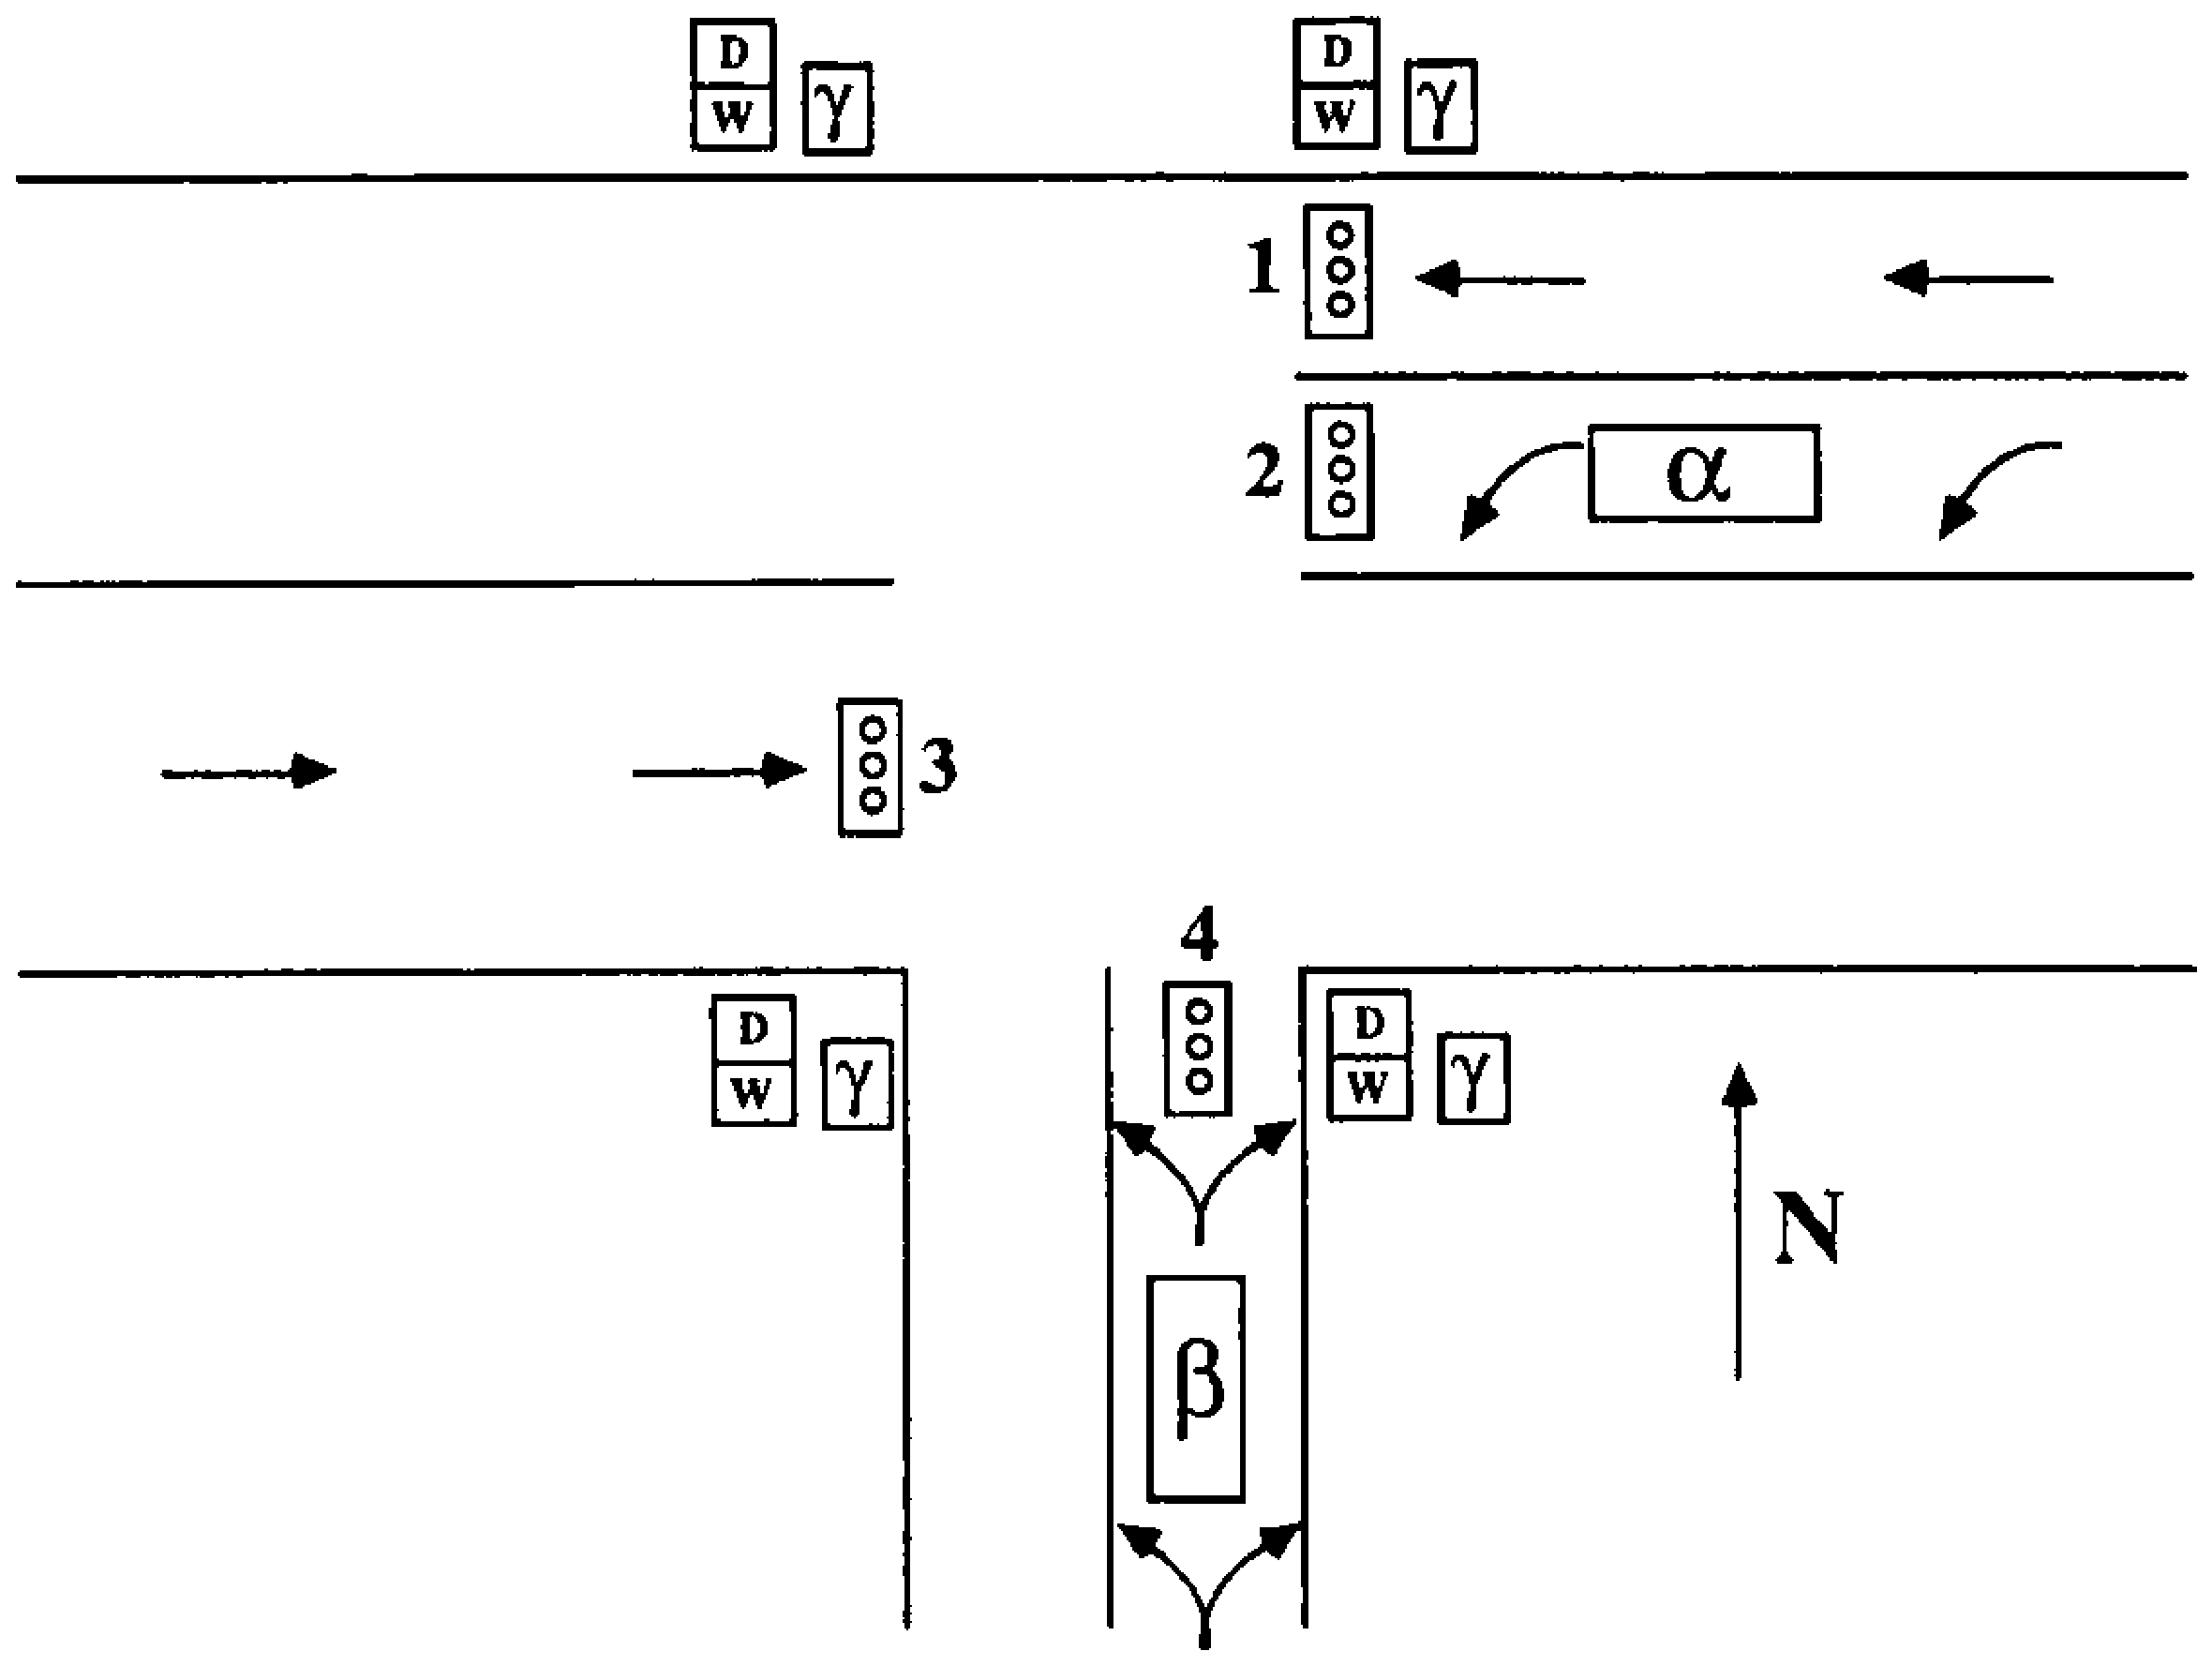
\epsfig{figure=ToFAfigures/fig7-19.eps,width=4.5in}}
\caption{The intersection discussed in Exercise 7.39}\label{fig-7.19}
\end{figure}
\begin{enumerate}
\item Define the new input and output alphabets.
\item Draw a Moore machine that implements this scenario.
\item Draw a Mealy machine that implements this scenario.
\end{enumerate}

\item Consider an intersection similar to that described in Example 7.16, as
shown in Figure \ref{fig-7.20}. There are now four left-turn signals in addition to the
four straight-ahead signals and additional input sensors $\gamma$ and $\delta$
for the other left-turn lanes. Assume that a normal alternation of
straight-ahead traffic is carried out, with no left turns indicated unless the
corresponding sensor is activated. Further assume that left-turn traffic will be
allowed to precede the opposing traffic.
\begin{enumerate}
\item Define the new input and output alphabets.
\item Draw a Moore machine that implements this scenario.
\item Draw a Mealy machine that implements this scenario.
\end{enumerate}
% Figure 7.20
\begin{figure}
\centerline{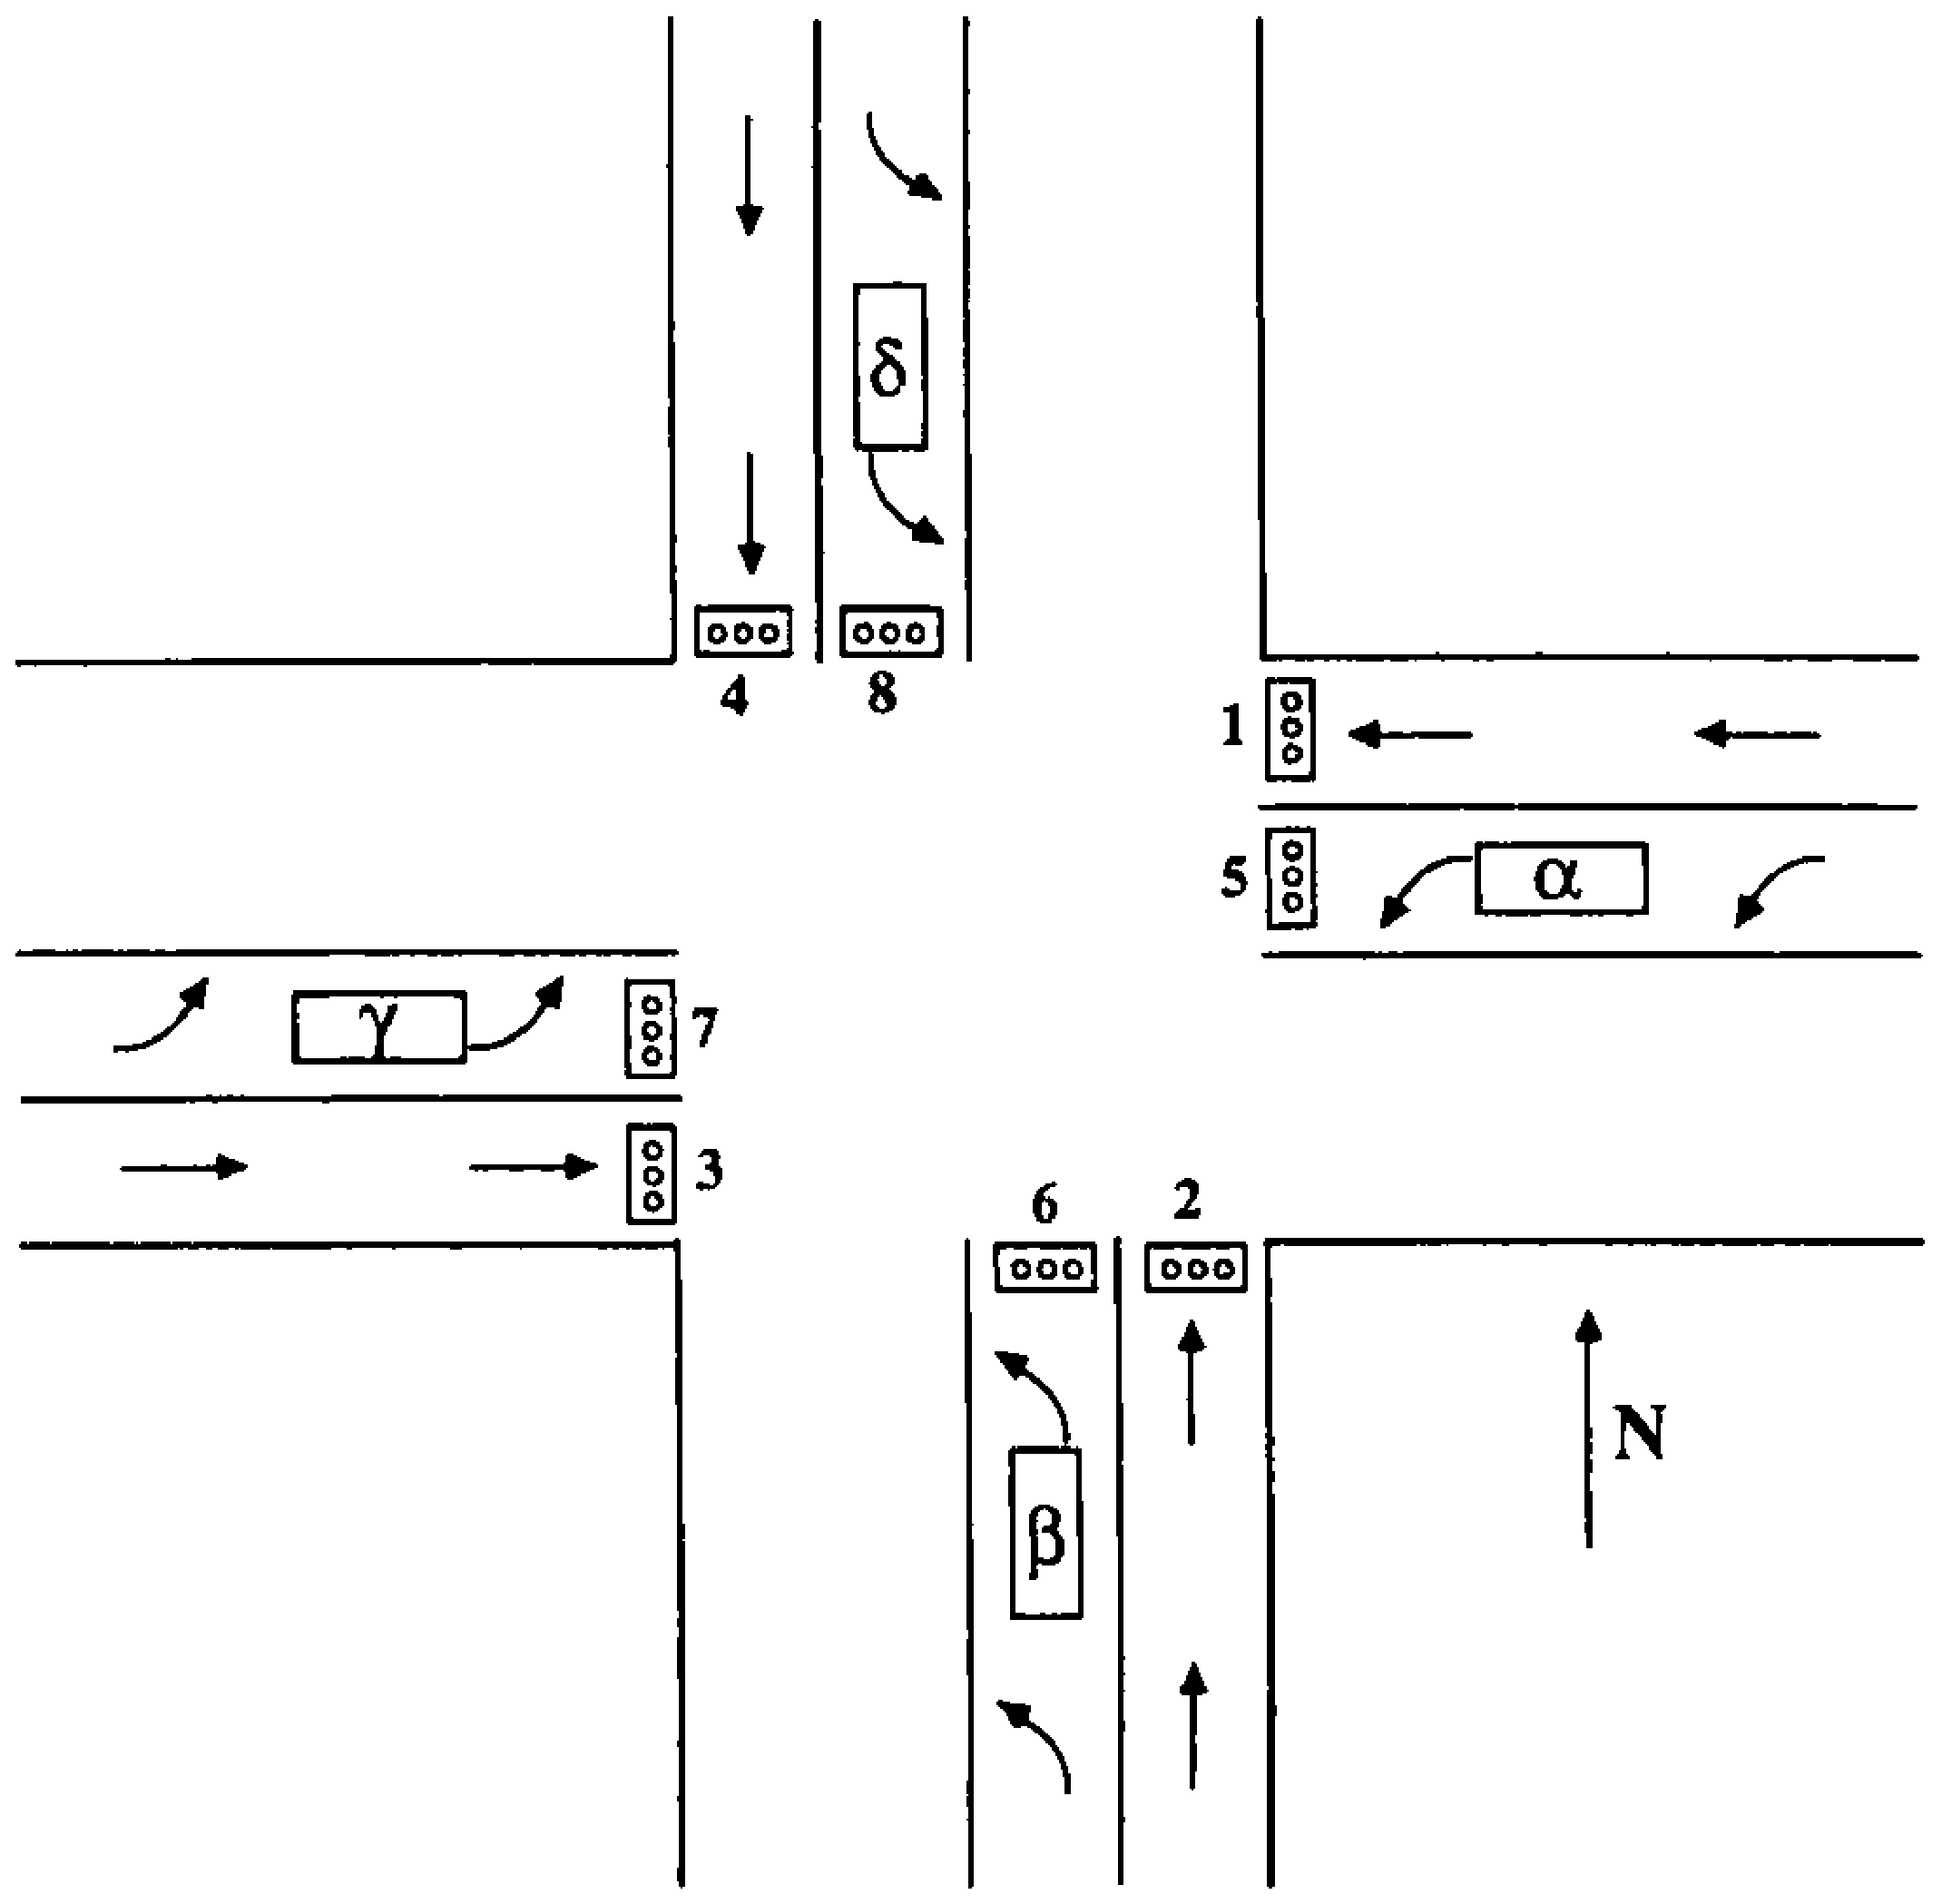
\epsfig{figure=ToFAfigures/fig7-20.eps,width=4.5in}}
\caption{The intersection discussed in Exercise 7.40}\label{fig-7.20}
\end{figure}

\item Consider an adder similar to the one in Example 7.15, but which instead
models addition in base 3.
\begin{enumerate}
\item Define the input and output alphabets.
\item Draw a Mealy machine that performs this addition.
\item Draw a Moore machine that performs this addition.
\item Draw a circuit that will implement the transducer built in part (b); use
both \<EOS\> and \<SOS\>.
\end{enumerate}

\item Consider an adder similar to the one in Example 7.15, but which models
addition in base 10.
\begin{enumerate}
\item Define the input and output alphabets.
\item Define the sextuple of a Mealy machine that performs this addition (by
indicating the output and transitions by concise formulas, rather than writing
out the 200 entries in the tables).
\item Define the sextuple of a Moore machine that performs this addition.
\item Draw a circuit that will implement the transducer built in part (b); use
both \<EOS\> and \<SOS\>.
\end{enumerate}

\item Consider a function $f_4$ implementing addition in a manner similar to
the function described by the transducer in Example 7.15, but that scans the
characters (that is, columns of digits) from left to right (rather than right to
left as in Example 7.15). Argue that $f_4$ is not FTD.

\item Given a MSM $M$, prove the following statements from Theorem \ref{thm-7.9}:
\begin{enumerate}
\item $M/\!\!_{E_M}$ is equivalent to $M$.
\item $M/\!\!_{E_M}$ is reduced.
\item If $M$ is connected, so is $M/\!\!_{E_M}$.
\end{enumerate}

\item Given a FTD function $f$, prove that the minimal Moore machine
corresponding to $f$ must be reduced.

\item Given a MSM $M$, prove the following statements from Theorem \ref{thm-7.10}:
\begin{enumerate}
\item A necessary and sufficient condition for $M$ to be minimal is that $M$ is
both reduced and connected.
\item $M^c/\!\!_{E_{M^c}}$ is minimal.
\end{enumerate}

\item Given MSMs $A=\langle\Sigma,\Gamma,S_A,s_{0_A},\delta_A,\omega_A\rangle$
and $B=\langle\Sigma,\Gamma,S_B,s_{0_B},\delta_B,\omega_B\rangle$, and a
homomorphism $\mu$$:\ S_A \rightarrow S_B$, prove the following statements from
Lemma \ref{lmm-7.5} and Corollary \ref{cor-7.9}:
\begin{enumerate}
\item $(\forall s \in S_A)(\forall x \in \Sigma^*)(\mu(\DBAR_A(s,x)) =
	\DBAR_B(\mu(s),x))$.
\item $(\forall s \in S_A)(\forall x \in \Sigma^*)(\OBAR_A(s,x) =
	\OBAR_B(\mu(s),x)))$.
\item $A$ is equivalent to $B$; that is, $f_A = f_B$.
\end{enumerate}

\item Prove Corollary \ref{cor-7.10}.

\item Prove Corollary \ref{cor-7.11}.

\item Given a FST $M=\langle\Sigma,\Gamma,S,s_0,\delta,\omega\rangle$ and
$M/\!\!_{E_M}=\langle\Sigma,\Gamma,S_{E_M},s_{0_{E_M}},\delta_{E_M},\omega_{E_M}
\rangle$ defined by
\begin{center}\begin{tabular}{ll}
$S_{E_M} =\{[s]_{E_M}$ $|$ $s \in S\}$ \\
$s_{0_{E_M}} = [s_0]_{E_M}$
\end{tabular}\end{center}
$\delta_{E_M}$ is defined by
\[ (\forall a \in \Sigma)(\forall [s]_{E_M} \in S_{E_M})(\delta_{E_M}([s]_{E_M},
	\pmb{a}) = [\delta(s,\pmb{a})]_{E_M}) \]
and $\omega_{E_M}$ is defined by
\[ (\forall\pmb{a}\in\Sigma)(\forall [s]_{E_M} \in S_{E_M})(\omega_{E_M}
	([s]_{E_M},\pmb{a}) = \omega(s,\pmb{a})) \]
\begin{enumerate}
\item Show that $\delta_{E_M}$ is well defined.
\item Show that $\omega_{E_M}$ is well defined.
\end{enumerate}

\item Given a MSM $M=\langle\Sigma,\Gamma,S,s_0,\delta,\omega\rangle$ and
$M/\!\!_{E_M}=\langle\Sigma,\Gamma,S_{E_M},s_{0_{E_M}},\delta_{E_M},\omega_{E_M}
\rangle$ defined by
\begin{center}\begin{tabular}{ll}
$S_{E_M} =\{[s]_{E_M}$ $|$ $s \in S\}$ \\
$s_{0_{E_M}} = [s_0]_{E_M}$
\end{tabular}\end{center}
$\delta_{E_M}$ is defined by
\[ (\forall a \in \Sigma)(\forall [s]_{E_M} \in S_{E_M})(\delta_{E_M}([s]_{E_M},
	\pmb{a}) = [\delta(s,\pmb{a})]_{E_M}) \]
and $\omega_{E_M}$ is defined by
\[ (\forall [s]_{E_M} \in S_{E_M})(\omega_{E_M}([s]_{E_M}) = \omega(s)) \]
\begin{enumerate}
\item Show that $\delta_{E_M}$ is well defined.
\item Show that $\omega_{E_M}$ is well defined.
\end{enumerate}

\item Consider the following assertion: If there is an isomorphism from $A$ to
$B$ and $A$ is connected, then $B$ must also be connected.
\begin{enumerate}
\item Prove that this is true for isomorphisms between Mealy machines.
\item Prove that this is true for isomorphisms between Moore machines.
\end{enumerate}

\item Consider the following assertion: If there is an isomorphism from $A$ to
$B$ and $B$ is connected, then $A$ must also be connected.
\begin{enumerate}
\item Prove that this is true for isomorphisms between Mealy machines.
\item Prove that this is true for isomorphisms between Moore machines.
\end{enumerate}

\item Consider the following assertion: If there is a homomorphism from $A$ to
$B$ and $A$ is connected, then $B$ must also be connected.
\begin{enumerate}
\item Give an example of two Mealy machines for which this assertion is false.
\item Give an example of two Moore machines for which this assertion is false.
\end{enumerate}

\item Consider the following assertion: If there is a homomorphism from $A$ to
$B$ and $B$ is connected, then $A$ must also be connected.
\begin{enumerate}
\item Give an example of two Mealy machines for which this assertion is false.
\item Give an example of two Moore machines for which this assertion is false.
\end{enumerate}

\item Assume $A$ and $B$ are connected FSTs and that there exists an isomorphism
$\psi$ from $A$ to $B$ and an isomorphism $\mu$ from B to A. Prove that $\psi =
\mu^{-1}$.

\item Assume $A$ and $B$ are FSTs and there exists an isomorphism $\psi$ from
$A$ to $B$ and an isomorphism $\mu$ from $B$ to $A$. Give an example for which
$\psi \not= \mu^{-1}$.

\item Give an example of a three-state MSM for which $E_{0A}$ has only one
equivalence class. Is it possible for $E_{0A}$ to be different from $E_{1A}$ in
such a machine? Explain.

\item \begin{enumerate}
\item Give an example of a Mealy machine for which $M$ is \emph{not} connected
and $M/\!\!_{E_M}$ is not connected.
\item Give an example of a Mealy machine for which $M$ is \emph{not} connected
but $M/\!\!_{E_M}$ is connected.
\end{enumerate}

\item \begin{enumerate}
\item Give an example of a Moore machine for which $M$ is \emph{not} connected
and $M/\!\!_{E_M}$ is not connected.
\item Give an example of a Moore machine for which $M$ is \emph{not} connected
but $M/\!\!_{E_M}$ is connected.
\end{enumerate}

\item For a homomorphism $\mu$$:\ S_A \rightarrow S_B$ between two Mealy machines
\[ A=\langle\Sigma,\Gamma,S_A,s_{0_A},\delta_A,\omega_A\rangle\qquad\text{and}
	\qquad B=\langle\Sigma,\Gamma,S_B,s_{0_B},\delta_B,\omega_B\rangle, \]
prove $(\forall s,t \in S_A)(\mu(s) E_B \mu(t) \Leftrightarrow s E_A t)$.

\item For a homomorphism $\mu$$:\ S_A \rightarrow S_B$ between two Moore machines
\[ A=\langle\Sigma,\Gamma,S_A,s_{0_A},\delta_A,\omega_A\rangle\qquad\text{and}
	\qquad B=\langle\Sigma,\Gamma,S_B,s_{0_B},\delta_B,\omega_B\rangle, \]
prove $(\forall s,t \in S_A)(\mu(s) E_B \mu(t) \Leftrightarrow s E_A t)$.

\item \begin{enumerate}
\item Give an example of a FST for which $A$ is \emph{not} reduced and $A^c$ is
not reduced.
\item Give an example of a FST for which $A$ is \emph{not} reduced and $A^c$
\emph{is} reduced.
\end{enumerate}

\item \begin{enumerate}
\item Give an example of a MSM for which $A$ is \emph{not} reduced and $A^c$ is
not reduced.
\item Give an example of a MSM for which $A$ is \emph{not} reduced and $A^c$
\emph{is} reduced.
\end{enumerate}

\item Isomorphism ($\cong$) is a relation in the set of all Mealy machines.
\begin{enumerate}
\item Prove that $\cong$ is a symmetric relation; that is, formally justify that
if there is an isomorphism from $A$ to $B$ then there is an isomorphism from $B$
to $A$.
\item Prove that $\cong$ is a reflexive relation.
\item Show that if $f$ and $g$ are isomorphisms, then $f \circ g$ is also an
isomorphism (whenever $f \circ g$ is defined).
\item From the results of parts (a), (b), and (c) given above, prove that
$\cong$ is an equivalence relation over the set of all Mealy machines.
\item Show that homomorphism is {\em not} an equivalence relation over the set of all
Mealy machines.
\end{enumerate}

\item \begin{enumerate}
\item Prove that $\cong$ is an equivalence relation in the set of all Moore
machines.
\item Show that homomorphism is {\em not} an equivalence relation over the set of all
Moore machines.
\end{enumerate}

\item Given a Mealy machine $M=\langle\Sigma,\Gamma,S,s_0,\delta,\omega\rangle$,
prove that there exists a homomorphism $\mu$ from $M$ to $M/\!\!_{E_M}$.

\item Given a Moore machine $M=\langle\Sigma,\Gamma,S,s_0,\delta,\omega\rangle$,
prove that there exists a homomorphism $\mu$ from $M$ to $M/\!\!_{E_M}$.

\item Consider the intersection presented in Example 7.16 and note that the
construction presented in Figure \ref{fig-7.15} prevents the transducer from leaving $s_2$
or $s_6$ while the appropriate sensor is active. The length of time spent in
each output configuration can be limited by replacing $s_2$ with a sequence of
states that ensures that the output configuration will change within, say, three
clock cycles (this is similar to the spirit in which $s_8$ was added). A similar
expansion can be made with regard to $s_6$. While this would not be a likely
problem if the side street were not heavily traveled, higher traffic situations
would require a different solution than that shown in Figure \ref{fig-7.15}.
\begin{enumerate}
\item Modify Figure \ref{fig-7.15} so that the output configuration can, when necessary,
remain at $\langle R,R,R,G\rangle$ for three clock cycles, but not for four
clock cycles.
\item Starting with the larger transducer found in part (a), make a similar
expansion to $s_6$.
\item Starting with the larger transducer found in part (a), make an expansion
to $s_6$ in such a way that the left-turn signal is guaranteed to be green for a
minimum of two clock cycles and a maximum of four clock cycles.
\end{enumerate}

\item Consider the intersection presented in Example 7.16 and note that the
construction presented in Figure \ref{fig-7.15} prevents the transducer from returning to
$s_0$ while either of the sensors is active. Thus, even if the length of time
spent in each output configuration was limited (see Exercise 7.69), left-turn
and northbound traffic could perpetually alternate without ever allowing the
east-west traffic to resume. This would not be a likely problem if the side
street were not heavily traveled, but higher traffic situations would require a
different solution than the one presented in Example 7.16.
\begin{enumerate}
\item Without adding any states to Figure \ref{fig-7.15}, modify the state transition
diagram so that east-west traffic will receive a green light occasionally.
\item By adding new states to Figure \ref{fig-7.15} (to remember the last lanes that had
the right of way), implement a controller that will ensure that no lane will get
a second green light if any other lane that has an active sensor has yet to
receive a green light. (It may be helpful to think of the east-west traffic as
having an implicit sensor that is always actively demanding service).
\end{enumerate}

\item Prove that if two Moore machines are homomorphic then they are equivalent.

\item Show that, for any FTD function $f$$:\ \Sigma^* \rightarrow \Sigma^*$,
\DSIG\ is closed under $f$.
\end{enumerate}

% Chapter, Section, Figure, Table, Theorem, Corollary, Lemma, Definition, {\bf 
\chapter{Regular Grammars}\label{ch-8}

In the preceding chapters, we have seen several ways to characterize the set
of FAD languages: via DFAs, NDFAs, right congruences, and regular expressions.
In this chapter we will look at still another way to represent this class, using
the concept of \emph{\Index{grammars}}. This construct is very powerful, and
many restrictions must be placed on the general definition of a grammar in order
to limit the scope to FAD languages. The very restrictive \emph{regular}
grammars will be explored in full detail in this chapter. The more robust
classes of grammars introduced here will be discussed at length in later
chapters.

\section{Overview Of The Grammar Hierarchy}\label{sec-8.1}

Much like the rules given in Backus-Naur Form (BNF) in Chapters \ref{ch-0} and \ref{ch-1}, the
language-defining power of a grammar stems from the generation of strings
through the successive replacement of symbols in a partially constructed string.
These replacement rules form the foundation for the definition of programming
languages and are used in compiler construction not only to determine correct
syntax, but also to help determine the \emph{meaning} of the statements and
thereby guide the translation of a program into machine language.

\subsection*{Example 8.1}

A BNF that describes the set of all valid FORTRAN identifiers is given below.
Recall that such identifiers must begin with a letter and be followed by no
more than five other letters and numerals. These criteria can be specified by
the following set of rules.
\begin{center}\begin{tabular}{r@{:: = }l}
$S$ & $\pmb{a}S_1|\pmb{b}S_1| \ldots |\pmb{z}S_1|\pmb{a}|\pmb{b}| \ldots
	|\pmb{z}$ \\
$S_1$ & $\pmb{a}S_2|\pmb{b}S_2| \ldots |\pmb{z}S_2|\pmb{a}|\pmb{b}| \ldots
	|\pmb{z}|\pmb{0}S_2|\pmb{1}S_2|\pmb{2}S_2| \ldots |\pmb{9}S_2|\pmb{0}|
	\pmb{1}|\pmb{2}| \ldots |\pmb{9}$ \\
$S_2$ & $\pmb{a}S_3|\pmb{b}S_3| \ldots |\pmb{z}S_3|\pmb{a}|\pmb{b}| \ldots
	|\pmb{z}|\pmb{0}S_3|\pmb{1}S_3|\pmb{2}S_3| \ldots |\pmb{9}S_3|\pmb{0}|
	\pmb{1}|\pmb{2}| \ldots |\pmb{9}$ \\
$S_3$ & $\pmb{a}S_4|\pmb{b}S_4| \ldots |\pmb{z}S_4|\pmb{a}|\pmb{b}| \ldots
	|\pmb{z}|\pmb{0}S_4|\pmb{1}S_4|\pmb{2}S_4| \ldots |\pmb{9}S_4|\pmb{0}|
	\pmb{1}|\pmb{2}| \ldots |\pmb{9}$ \\
$S_4$ & $\pmb{a}S_5|\pmb{b}S_5| \ldots |\pmb{z}S_5|\pmb{a}|\pmb{b}| \ldots
	|\pmb{z}|\pmb{0}S_5|\pmb{1}S_5|\pmb{2}S_5| \ldots |\pmb{9}S_5|\pmb{0}|
	\pmb{1}|\pmb{2}| \ldots |\pmb{9}$ \\
$S_5$ & $\pmb{a}|\pmb{b}| \ldots |\pmb{z}|\pmb{0}|\pmb{1}|\pmb{2}| \ldots 
	|\pmb{9}$
\end{tabular}\end{center}
The first rule specifies that $S$ can be replaced by any of the 26 letters of
the Roman alphabet or any such letter followed by the token $S_1$. These
\emph{\Index{productions}} (rules) do indeed define the variable names found in
FORTRAN programs. Starting with $S$, a derivation might proceed as $S \Rightarrow
\pmb{s}S_1 \Rightarrow \pmb{su}S_2 \Rightarrow \pmb{sum}$, indicating that \pmb{sum}
is a valid FORTRAN identifier. Invalid identifiers, such as $\pmb{2a}$, cannot
be derived from these productions by starting with $S$.

\subsection*{Example 8.2}

The strings used to represent regular sets (see Chapter \ref{ch-6}) could have been
succinctly specified using BNF. Recall that regular languages over, say,
$\{\pmb{a},\pmb{b},\pmb{c}\}$ are described by regular expressions. These
regular expressions were strings over the alphabet $\{\pmb{\emptyset},
\pmb{\epsilon},\pmb{a},\pmb{b},\pmb{c},\pmb{\cup},\pmb{\cdot},\pmb{^*},\pmb{)},
\pmb{(}\}$, and the formal definition was quite complex. A regular expression
over $\{\pmb{a},\pmb{b},\pmb{c}\}$ was defined to be a sequence of symbols
formed by repeated application of the following rules:
\begin{enumerate}[i.]
\item $\pmb{a}$, $\pmb{b}$, $\pmb{c}$ are each regular expressions.
\item $\emptyset$ is a regular expression.
\item $\epsilon$ is a regular expression.
\item If $R_1$ and $R_2$ are regular expressions, then so is $\pmb{(}R_1 \pmb\cdot R_2\pmb{)}$.
\item If $R_1$ and $R_2$ are regular expressions, then so is $\pmb{(}R_1 \pmb\cup R_2\pmb{)}$.
\item If $R_1$ is a regular expression, then so is $R^{\pmb *}_1$.
\end{enumerate}
The conditions set forth above could have instead been succinctly specified by
the BNF shown below.
\[ R:: =\pmb{a}|\pmb{b}]\pmb{c}|\pmb{\epsilon}|\pmb{\emptyset}|\pmb{(}R\pmb\cdot R\pmb{}|\pmb{(}R\cup R\pmb{)}|R^{\pmb *} \]
The following is a typical derivation, culminating in the regular expression
$\pmb{(a\pmb\cdot(c\pmb\cup\epsilon))^{\pmb *}}$
\begin{center}\begin{tabular}{r@{ $\Rightarrow$ }l}
$R$ & $R^{\pmb *}$ \\
& $\pmb{(}R \pmb\cdot R\pmb{)}^{\pmb *}$ \\
& $\pmb{(}\pmb{a} \pmb\cdot R\pmb{)}^{\pmb *}$ \\
& $\pmb{(}\pmb{a}\pmb\cdot\pmb{(}R \pmb\cup R\pmb{)}\pmb{)}^{\pmb *}$ \\
& $\pmb{(}\pmb{a}\pmb\cdot\pmb{(}\pmb{c}\pmb\cup R\pmb{)}\pmb{)}^{\pmb *}$ \\
& $\pmb{(}\pmb{a}\pmb\cdot\pmb{(}\pmb{c}\pmb\cup\pmb{\epsilon}\pmb{)}\pmb{)}^{\pmb *}$
\end{tabular}\end{center}
Note that in the intermediate steps of the derivation, we do not wish to consider
strings such as $(\pmb{a}\cdot R)^*$ to be valid regular expressions. $(\pmb{a}
\cdot R)^*$ is not a string over the alphabet $\{\pmb{\emptyset},\pmb{\epsilon},
\pmb{a},\pmb{b},\pmb{c},\pmb{\cup},\pmb{\cdot},\pmb{^*},\pmb{)},\pmb{(}\}$, and
it does not represent a regular language over $\{\pmb{a},\pmb{b},\pmb{c}\}$. To
generate a valid regular expression, the derivation \emph{must} proceed until
all occurrences of $R$ are removed. To differentiate between the symbols that
may remain and those that must be replaced, grammars divide the tokens into
\emph{\Index{terminal}} symbols and \emph{\Index{nonterminal}} symbols,
respectively.

The following notational conventions will be used throughout the remainder of
the text. Members of $\Sigma$, will be represented by lowercase roman letters
such as $\pmb{a}$, $\pmb{b}$, $\pmb{c}$, $\pmb{d}$ and will be referred to as
\emph{terminal} symbols. A new alphabet $\Omega$ will be introduced, and its
members will be represented by uppercase roman letters such as $A$, $B$, $C$,
and $S$, and these will be called \emph{nonterminal} symbols. $S$ will often
denote a special nonterminal, called the \emph{start} symbol. The specification
of the production rules will be somewhat different from the BNF
examples given above. The common grammatical notation for rules such as $S:: =
\pmb{a}S_1$ and $S:: = \pmb{b}S_1$ is $S \rightarrow \pmb{a}S_1$ and $S
\rightarrow \pmb{b}S_1$. As with BNF, a convenient shorthand notation for a
group of productions involves the use of the $|$ (\emph{or}) symbol. The
productions $Z \rightarrow \pmb{aa}B$, $Z \rightarrow \pmb{ac}$, $Z \rightarrow
\pmb{cb}T$, which all denote replacements for $Z$, could be succinctly
represented by $Z \rightarrow \pmb{aa}B|\pmb{ac}|\pmb{cb}T.$

A production can be thought of as a replacement rule; that is, $A \rightarrow
\pmb{cdba}$ indicates that occurrences of the (nonterminal) $A$ can be replaced
by the string $\pmb{cdba}$. For example, the string $\pmb{ab}B\underline{A}\pmb{d}B\pmb{c}$ can
be transformed into the string $\pmb{ab}B\pmb{\underline{cdba}d}B\pmb{c}$ by applying the
production $A \rightarrow \pmb{cdba}$; we will write
\[ \pmb{ab}BA\pmb{d}B\pmb{c} \Rightarrow \pmb{ab}B\pmb{cdbad}B\pmb{c}, \]
and say that $\pmb{ab}B\pmb{cdbad}B\pmb{c}$ was derived (in one step) from $\pmb{ab}BA\pmb{d}B\pmb{c}$.
Productions may be applied in succession; for example, if both $A \rightarrow
\pmb{cdba}$ and $B \rightarrow \pmb{ef}B$ were available, then the following
modifications of the string $\pmb{ab}BA\pmb{d}B\pmb{c}$ would be possible: $\pmb{ab}BA\pmb{d}B\pmb{c}
\Rightarrow \pmb{ab}B\pmb{cdbad}B\pmb{c} \Rightarrow \pmb{abef}B\pmb{cdbad}B\pmb{c} \Rightarrow
\pmb{abefef}B\pmb{cdbad}B\pmb{c}$, and we might write $\pmb{ab}BA\pmb{d}B\pmb{c} \  \overline{\Rightarrow} \ 
\pmb{abefef}B\pmb{cdbad}B\pmb{c}$ to indicate that $\pmb{ab}BA\pmb{d}B\pmb{c}$ can produce $\pmb{
abefef}B\pmb{cdbad}B\pmb{c}$ in zero or more steps (three steps in this case). Note that the
distinction between $\Rightarrow$ and $\overline{\Rightarrow}$ is reminiscent of
the difference between the state transition functions $\delta$ and \DBAR. As
with the distinction between the transducer output functions $\omega$ and \OBAR,
the overbar is meant to indicate the result of successive applications of the
underlying operation. The symbol \  $\DRightarrow$ is often used in place
of $\overline{\Rightarrow}$.

As illustrated by Example 8.1, several nonterminals may be used in the grammar.
The set of nonterminals in the grammar given for FORTRAN identifiers was
comprised of $\{S,S_1,S_2,S_3,S_4,S_5\}$. The start symbol designates which of
these nonterminals should always be used to begin derivations.

The previous examples discussed in this section have illustrated all the
essential components of a grammar. A grammar must specify the terminal alphabet,
the set of intermediary nonterminal symbols, and the designated start symbol,
and it must also enumerate the set of rules for replacing phrases within a
derivation with other phrases. In the above examples, the productions have all
involved the replacement of single nonterminals with other strings. In an
unrestricted grammar, a general replacement rule may allow an entire string
$\alpha$ to be replaced by another string $\beta$.
Thus, $\pmb{a}B\pmb{c}D \rightarrow \pmb{be}A$
would be a legal production, and thus whenever the sequence $\pmb{a}B\pmb{c}D$
is found within a derivation it can be replaced by the shorter
string $\pmb{be}A$.

% Definition 8.1
\begin{dfn}\label{dfn-8.1}
An \emph{\Index{unrestricted}} or \emph{\Index{type 0 grammar}} over an alphabet
$\Sigma$ is a quadruple $G=\langle\Omega,\Sigma,S,P\rangle$, where:
\begin{center}\begin{tabular}{l}
$\Omega$ is a (nonempty) set of \emph{nonterminals}. \\
$\Sigma$ is a (nonempty) set of \emph{terminal symbols} (and $\Omega\cap\Sigma =
	\emptyset$). \\
$S$ is the designated \emph{start symbol} (and $S \in \Omega$). \\
$P$ is a set of \emph{productions} of the form $\alpha\rightarrow\beta$, where
	$\alpha\in(\Omega\cup\Sigma)^+, \beta\in(\Omega\cup\Sigma)^*$.
\end{tabular}\end{center}
\end{dfn}

\subsection*{Example 8.3}

Consider the grammar
\[ G'' = \langle\{A,B,S,T\},\{\pmb{a},\pmb{b},\pmb{c}\},S,\{S\rightarrow\pmb{a}
	SB\pmb{c},S\rightarrow T,T\rightarrow\lambda,TB\rightarrow\pmb{b}T,
	\pmb{c}B\rightarrow B\pmb{c}\}\rangle \]
A typical derivation, starting from the start state S, would be:
\begin{center}\begin{tabular}{r@{ }c@{ }l}
$S$ & $\Rightarrow$ & (by applying $S \rightarrow \pmb{a}SB\pmb{c}$) \\
$\pmb{a}SB\pmb{c}$ & $\Rightarrow$ & (by applying $S \rightarrow \pmb{a}SB\pmb{c}$) \\
$\pmb{aa}SB\pmb{c}B\pmb{c}$ & $\Rightarrow$ & (by applying $S \rightarrow T$) \\
$\pmb{aa}TB\pmb{c}B\pmb{c}$ & $\Rightarrow$ & (by applying $TB \rightarrow \pmb{b}T$) \\
$\pmb{aab}T\pmb{c}B\pmb{c}$ & $\Rightarrow$ & (by applying $\pmb{c}B \rightarrow B\pmb{c}$) \\
$\pmb{aab}TB\pmb{cc}$ & $\Rightarrow$ & (by applying $TB \rightarrow \pmb{b}T$) \\
$\pmb{aabb}T\pmb{cc}$ & $\Rightarrow$ & (by applying $T \rightarrow \lambda$) \\\
$\pmb{aabbcc}$
\end{tabular}\end{center}
Depending on how many times the production $S \rightarrow \pmb{a}SB\pmb{c}$ is
used, this grammar will generate strings such as $\lambda$, $\pmb{abc}$,
$\pmb{aabbcc}$, and $\pmb{aaabbbccc}$. The set of strings that can be generated
by this particular grammar is $\{\pmb{a}^i\pmb{b}^i\pmb{c}^i| i \geq 0\}$. In
this sense, each grammar defines a \emph{language}. Specifically, we require
that derivations start with the designated start symbol and proceed until only
members of $\Sigma$ remain in the resulting string.

% Definition 8.2
\begin{dfn}\label{dfn-8.2}\index{language!type $k$}
Given a grammar $G = \langle\Omega,\Sigma,S,P\rangle$, the \emph{language
generated by} $G$, denoted by $L(G)$, is given by $L(G)=\{x\ |\ x \in \Sigma^*\!
\wedge S\ \DRightarrow x\}$.
\end{dfn}

A language that can be defined by a type 0 grammar is called a \emph{type 0
language}. Thus, as shown by the grammar $G''$ given in Example 8.3, $L(G'')
=\{\pmb{a}^i\pmb{b}^i\pmb{c}^i|i \geq 0\}$ is a type 0 language.

The way grammars define languages is fundamentally different from the way
automata define languages. An automaton is a \emph{\Index{cognitive device}}, in that it
is used to directly decide whether a given string should be accepted into the
language. In contrast, a grammar is a \emph{\Index{generative device}}: the
productions specify how to generate all the words in the language represented by
the grammar, but do not provide an obvious means of determining whether a given
string can be generated by those rules. There are many applications in which it
is important to be able to determine whether a given string can be generated by
a particular grammar, and the task of obtaining cognitive answers from a
generative construct will be addressed at several points later in the text. The
reverse transformation, that is, producing an automaton that recognizes exactly
those strings that are generated by a given grammar, is addressed in the next
section.

The distinction between generative and cognitive approaches to representing
languages has been explored previously, when regular expressions were considered
in Chapter \ref{ch-6}. Regular expressions are also a generative construct, in the sense
that a regular expression can be used to begin to enumerate the words in the
corresponding regular set. As is the case with grammars, it is inconvenient to
use regular expressions in a cognitive fashion: it may be difficult to tell
whether a given string is among those represented by a particular regular
expression. Chapter \ref{ch-6} therefore explored ways to transform a regular expression
into a corresponding automaton. It is likewise feasible to define corresponding
automata for certain grammars (see Lemma \ref{lmm-8.2}). However, Example 8.3 illustrated
that some grammars produce non-FAD languages and therefore cannot possibly be
represented by deterministic finite automata. The translation from a mechanical
representation of a language to a grammatical representation is always
successful, in that every automaton has a corresponding grammar (Lemma \ref{lmm-8.1}).
This result is similar to Theorem \ref{thm-6.3}, which showed that every automaton has a
corresponding regular expression.

Note that in Example 8.3 the only production that specified that a string be
replaced by a shorter string was $T \rightarrow \lambda$. Consequently, the
length of the derived string either increased or remained constant except where
this last production was applied. Rules such as $\pmb{a}B\pmb{c}D \rightarrow
\pmb{be}A$, in which four symbols are replaced by only three, will at least
momentarily decrease the length of the string. Such productions are called
\emph{contracting} productions. Grammars that satisfy the added requirement that
no production may decrease the length of the derivation are called
\index{context-sensitive grammar}\emph{context sensitive}. Such grammars cannot generate as many
languages as the unrestricted grammars, but they have the added advantage of
allowing derivations to proceed in a more predictable manner. Programming
languages are explicitly designed to ensure that they can be represented by
grammars that are context sensitive.

% Definition 8.3
\begin{dfn}\label{dfn-8.3}\index{context-sensitive grammar (pure)}
A \emph{\Index{pure context-sensitive grammar}} over an alphabet $\Sigma$ is a
quadruple $G=\langle\Omega,\Sigma,S,P\rangle$, where:

\begin{quote}
$\Omega$ is a (nonempty) set of \emph{nonterminals}. \\
$\Sigma$ is a (nonempty) set of \emph{terminal symbols} (and $\Omega \cap \Sigma
	= \emptyset$). \\
$S$ is the designated \emph{start symbol} (and $S \in \Omega$). \\
$P$ is a set of \emph{productions} of the form $\alpha \rightarrow \beta$, where
	$\alpha \in (\Omega \cup \Sigma)^+$, $\beta \in (\Omega \cup \Sigma)^+$,
	and $|\alpha| \leq |\beta|$.
\end{quote}
\end{dfn}

In a derivation in a context-sensitive grammar, if $S \Rightarrow x_1
\Rightarrow x_2 \Rightarrow \ldots \Rightarrow x_n$, then we are assured that
$1 = |S| \leq |x_1| \leq |x_2| \leq \cdots \leq |x_n|$. Unfortunately, this
means that in a pure context-sensitive grammar it is impossible to begin with
the start symbol (which has length 1) and derive the empty string (which is of
length 0).

\subsection*{Example 8.4}

Languages that contain $\lambda$, such as $\{\pmb{a}^i\pmb{b}^i\pmb{c}^i|i \geq
0\}$ generated in Example 8.3 by the unrestricted grammar $G''$, cannot possibly
be represented by a pure context-sensitive grammar. However, the empty string is
actually the only impediment to finding an alternative collection of productions
that all satisfy the condition $|\alpha| \leq |\beta|$. The language
$\{\pmb{a}^i\pmb{b}^i\pmb{c}^i|i \geq 1\}$ can be represented by a pure
context-sensitive grammar, as illustrated by the following grammar. Let $G$ be
given by
\[ G = \langle\{A,B,S,T\},\{\pmb{a},\pmb{b},\pmb{c}\},S,\{S \rightarrow
	\pmb{a}SB\pmb{c},S \rightarrow \pmb{a}T\pmb{c}, T \rightarrow \pmb{b},
	TB \rightarrow \pmb{b}T, \pmb{c}B \rightarrow B\pmb{c}\}\rangle \]
The derivation to produce $\pmb{aabbcc}$ would now be
\begin{center}\begin{tabular}{r@{ }c@{ }l@{ }}
$S$ & $\Rightarrow$ & (by applying $S \rightarrow \pmb{a}SB\pmb{c}$) \\
$\pmb{a}SB\pmb{c}$ & $\Rightarrow$ & (by applying $S \rightarrow \pmb{a}T\pmb{c}$) \\
$\pmb{aa}T\pmb{c}B\pmb{c}$ & $\Rightarrow$ & (by applying $\pmb{c}B \rightarrow
	B\pmb{c}$) \\
$\pmb{aa}TB\pmb{cc}$ & $\Rightarrow$ & (by applying $TB \rightarrow \pmb{b}T$) \\
$\pmb{aab}T\pmb{cc}$ & $\Rightarrow$ & (by applying $T \rightarrow \pmb{b}$) \\
$\pmb{aabbcc}$
\end{tabular}\end{center}
The shortest string derivable by $G$ is $S \Rightarrow \pmb{a}T\pmb{c}
\Rightarrow \pmb{abc}$. In Example 8.3, the shortest derivation was $S
\Rightarrow T \Rightarrow \lambda$.

Any pure context-sensitive grammar can be modified to include $\lambda$ by
adding a new start state $Z$ and two new productions $Z \rightarrow \lambda$ and
$Z \rightarrow S$, where $S$ was the original start state. Such grammars and
their resulting languages are generally referred to as \emph{type 1} or
\emph{context sensitive}.

% Definition 8.4\index{language!type $k$}
\begin{dfn}\label{dfn-8.4}\index{context-sensitive grammar}
A \emph{context-sensitive} or \emph{\Index{type 1 grammar}} over an
alphabet $\Sigma$ is either a pure context-sensitive grammar or a quadruple
\[ G'=\langle\Omega\cup\{Z\},\Sigma,Z,P\cup\{Z\rightarrow\lambda,Z\rightarrow
	S\}\rangle, \]
where $G=\langle\Omega,\Sigma,S,P\rangle$ is a pure context-sensitive grammar
and $Z \notin \Omega\cup\Sigma$.
\end{dfn}

The only production $\alpha\rightarrow\beta$ that violates the condition
$|\alpha| \leq |\beta|$ is $Z\rightarrow\lambda$, and this production cannot
play a part in any derivation other than $Z\Rightarrow\lambda$. From the start
symbol $Z$, the application $Z\rightarrow\lambda$ immediately ends the
derivation (producing $\lambda$), while the application of $Z \rightarrow S$
will provide no further opportunity to use $Z\rightarrow\lambda$, since the
requirement that $Z\notin\Omega\cup\Sigma$ means that the other productions will
never allow $Z$ to reappear in the derivation. Thus, $G'$ enhances the generating
power of $G$ only to the extent that $G'$ can produce $\lambda$. Every string in
$L(G)$ can be derived from the productions of $G'$, and $G'$ generates no new
strings besides $\lambda$. This argument essentially proves that $L(G') = L(G)
\cup\{\lambda\}$ (see the exercises).

\subsection*{Example 8.5}

The language generated by $G''$ in Example 8.3 was $L(G'')=\{\pmb{a}^i\pmb{b}^i
\pmb{c}^i|i \geq 0\}$. Since $L(G'')$ is $\{\pmb{a}^i\pmb{b}^i\pmb{c}^i|i\geq
1\}\cup\{\lambda\}$, it can therefore be represented by a context-sensitive
grammar by modifying the pure context-sensitive grammar in Example 8.4. Let $G'$
be given by
\begin{center}\begin{tabular}{r@{ }l}
$G' =$ & $\langle\{A,B,S,T,Z\},\{\pmb{a},\pmb{b},\pmb{c}\},Z,$ \\
& $\{S\rightarrow\pmb{a}SB\pmb{c},S\rightarrow\pmb{a}T\pmb{c},T\rightarrow\pmb{b},
	TB\rightarrow\pmb{b}T,\pmb{c}B\rightarrow B\pmb{c},Z\rightarrow\lambda,
	Z \rightarrow S\}\rangle$
\end{tabular}\end{center}
The derivation to produce $\pmb{aabbcc}$ would now be
\begin{center}\begin{tabular}{r@{ }c@{ }l@{ }}
$Z$ & $\Rightarrow$ & (by applying $Z \rightarrow S$) \\
$S$ & $\Rightarrow$ & (by applying $S \rightarrow \pmb{a}SB\pmb{c}$) \\
$\pmb{a}SB\pmb{c}$ & $\Rightarrow$ & (by applying $S \rightarrow \pmb{a}T\pmb{c}$) \\
$\pmb{aa}T\pmb{c}B\pmb{c}$ & $\Rightarrow$ & (by applying $\pmb{c}B \rightarrow
	B\pmb{c}$) \\
$\pmb{aa}TB\pmb{cc}$ & $\Rightarrow$ & (by applying $TB \rightarrow \pmb{b}T$) \\
$\pmb{aab}T\pmb{cc}$ & $\Rightarrow$ & (by applying $T \rightarrow \pmb{b}$) \\
$\pmb{aabbcc}$
\end{tabular}\end{center}
This grammar does produce $\lambda$, but all other derivations are strictly
length-increasing. Note that this was not the case in the grammar $G''$ in
Example 8.3. The last step of the derivation shown there transformed a string of
length 7 into a string of length 6. $G''$ does not satisfy the definition of a
context-sensitive grammar; even though only $T$ could produce $\lambda$, $T$
could occur later in the derivation. The presence of $T$ at later steps destroys
the desirable property of having all other derivations strictly length-increasing
at each step. Definition \ref{dfn-8.4} is constructed to ensure that the start symbol $Z$
can never appear in a later derivation step.

The restriction of productions to nondecreasing length reduces the number of
languages that can be generated; as discussed in later chapters, there exist
type 0 languages that cannot be generated by any type 1 grammar. The restriction
also allows arguments about the derivation process to proceed by induction on
the number of symbols in the resulting terminal string and is crucial to the
development of \emph{\Index{normal forms}} for context-sensitive grammars.

We have already seen examples of different grammars generating the same set
of words, as in the grammars $G''$and $G'$ from Examples 8.3 and 8.5. The term
context sensitive comes from the fact that context-sensitive languages (that
is, type 1 languages) can be represented by grammars in which the productions
are all of the form $\alpha B\gamma\rightarrow\alpha\beta\gamma$, where a single
nonterminal $B$ is replaced by the string $\beta$ in the \emph{context} of the strings
$\alpha$ on the left and $\gamma$ on the right. Specialized grammars such as
these, in which there are restrictions on the form of the productions, are
examples of \emph{normal forms} and are discussed later in the text.

If the productions in a grammar all imply that single nonterminals can be
replaced without regard to the context, then the grammar is called
\emph{\Index{context free}}. In essence, this means that all productions are of
the form $A\rightarrow\beta$, where the left side is just a single nonterminal
and the right side is an arbitrary string. The resulting languages are also
called \emph{type 2} or \emph{context free}.

% Definition 8.5
\begin{dfn}\label{dfn-8.5}\index{language!type $k$}
A \emph{\Index{pure context-free grammar}} over an alphabet $\Sigma$ is a
quadruple $G=\langle\Omega,\Sigma,S,P\rangle$, where:

\begin{quote}
$\Omega$ is a (nonempty) set of \emph{nonterminals}. \\
$\Sigma$ is a (nonempty) set of \emph{terminal symbols} (and $\Omega\cap\Sigma =
	\emptyset$). \\
$S$ is the designated \emph{start symbol} (and $S\in\Omega$). \\
$P$ is a set of \emph{productions} of the form $A\rightarrow\beta$, where $A\in\Omega,
	\beta\in(\Omega\cup\Sigma)^+$.
\end{quote}
\end{dfn}
Note that since the length of the left side of a context-free production is 1
and the right side cannot be empty, pure context-free grammars have no
contracting productions and are therefore pure context-sensitive grammars. As
with pure context-sensitive grammars, pure context-free grammars cannot generate
languages that contain the empty string.

% Definition 8.6
\begin{dfn}\label{dfn-8.6}
A \emph{context-free} or \emph{\Index{type 2 grammar}} over an alphabet $\Sigma$
is either a pure context-free grammar or a quadruple
\[ G' = \langle\Omega\cup\{Z\},\Sigma,Z,P\cup\{Z\rightarrow\lambda,Z\rightarrow
	S\}\rangle, \]
where $G=\langle\Omega,\Sigma,S,P\rangle$ is a pure context-free grammar and
$Z \notin \Omega\cup\Sigma$.
\end{dfn}

Productions of the form $C\rightarrow\beta$ are called \emph{\Index{C-rules}}.
As was done with context-sensitive grammars, this definition uses a new start
state $Z$ to avoid all such length-decreasing productions except for a single
one of the form $Z\rightarrow\lambda$, which is used only for generating the
empty string. Type 2 languages will therefore always be type 1 languages. Note
that the definition ensures that the only production that can decrease the
length of a derivation must be the Z-rule $Z\rightarrow\lambda$.

The grammar corresponding to the BNF given in Example 8.2 would be a
context-free grammar, and thus the collection of all regular expressions is a
type 2 language. The grammar given in Example 8.4 is not context free due to the
presence of the production $\pmb{c}B\rightarrow B\pmb{c}$, but this does not
yield sufficient evidence to claim that the resulting language $\{\pmb{a}^i
\pmb{b}^i\pmb{c}^i|i\geq 1\}$ is not a context-free language. To support this
claim, it must be shown that \emph{no} type 2 grammar can generate this language.
A pumping lemma for context-free languages will be presented in Chapter \ref{ch-10} to
provide a tool for measuring the complexity of such languages. Just as there
are type 1 languages that are not type 2, there are type 0 languages that are
not type 1.\index{hierarchy!of grammars}

Note that even these very restrictive type 2 grammars can produce languages
that are not FAD. As shown in Example 8.2, the language consisting of the
collection of all strings representing regular expressions is context free.
However, this collection is \emph{not} FAD, since it is clear that the pumping
lemma (Theorem \ref{thm-2.3}) would show that a DFA could not hope to correctly match up
unlimited pairs of parentheses.

Consequently, even more severe restrictions must be placed on grammars if they
are to have generative powers similar to the cognitive powers of a deterministic
finite automaton. The type 3 grammars explored in the next section are precisely
what is required. It will follow from the definitions that all type 3 languages
are type 2. It is likewise clear that all type 2 languages must be type 1, and
every type 1 language is type 0. Thus, a \emph{hierarchy}\index{hierarchy!of grammars} of languages is formed,
from the most restrictive type 3 languages to the most robust type 0 languages.
The four classes of languages are distinct; there are type 2 languages that are
not type 3 (for example, Example 8.2), type 1 languages that are not type 2 (see
Chapter \ref{ch-9}), and type 0 languages that are not type 1 (see Chapter \ref{ch-12}).

\section{Right-Linear Grammars and Automata}\label{sec-8.2}

The grammatical classes described in Section \ref{sec-8.1} are each capable of generating
all the FAD languages; indeed, they even generate languages that cannot be
recognized by finite automata. This section will explore a class of grammars
that generate the class of regular languages: every FAD language can be
generated by one of the right-linear grammars defined below, and yet no
right-linear grammar can generate a non-FAD language.

% Definition 8.7
\begin{dfn}\label{dfn-8.7}\index{language!type $k$}
A \emph{\Index{right-linear grammar}} over an alphabet $\Sigma$ is a quadruple
$G=\langle\Omega,\Sigma,S,P\rangle$, where

\begin{quote}
$\Omega$ is a (nonempty) set of \emph{nonterminals}. \\
$\Sigma$ is a (nonempty) set of \emph{terminal symbols} (and $\Omega\cap\Sigma =
	\emptyset$). \\
$S$ is the designated \emph{start symbol} (and $S\in\Omega$). \\
$P$ is a set of \emph{productions} of the form $A\rightarrow xB$, where $A\in\Omega, B
	\in(\Omega\cup\lambda)$, and $x\in\Sigma^*$
\end{quote}
\end{dfn}

Right-linear grammars belong to the class of type 3 grammars and generate all
the type 3 languages. Grammars that are right linear are very restrictive;
only one nonterminal can appear, and it must appear at the very end of the
expression. Consequently, in the course of a derivation, new terminals appear
only on the right end of the developing string, and the only time the string
might shrink in size is when a (final) production of the form $A \rightarrow
\lambda$ is applied. A right-linear grammar may have several contracting
productions that produce $\lambda$ and may not strictly conform with the
definition of a context-free grammar. However, Corollary \ref{cor-8.3} will show that
every type 3 language is a type 2 language.

Right-linear grammars generate words in the same fashion as the grammars
defined in Section \ref{sec-8.1}. The following definition of \emph{\Index{derivation}} is
tailored to right-linear grammars, but it can easily be generalized to less
restrictive grammars (see Chapter \ref{ch-9}).

% Definition 8.8
\begin{dfn}\label{dfn-8.8}
Let $G=\langle\Omega,\Sigma,S,P\rangle$ be a right-linear grammar, $y\in\Sigma^*$,
and $A \rightarrow xB$ be a production in $P$. We will say that $yxB$ can be
\emph{\Index{directly derive}d} from $yA$ by applying the production $A
\rightarrow xB$, and write $yA \Rightarrow yxB$. Furthermore, if
\[ (x_1A_1\Rightarrow x_2A_2) \wedge (x_2A_2\Rightarrow x_3A_3) \wedge \cdots
	\wedge (x_{n-1}A_{n-1}\Rightarrow x_nA_n), \]
where $x_i\in\Sigma^*$ for $i=1,2,\ldots,n,\ A_i\in\Omega$ for $i=1,2,\ldots,n-1$,
and $A_n\in(\Omega\cup\lambda)$, then we will say that $x_1A_1$ \emph{derives}
$x_nA_n$, and write $x_1A_1 \DRightarrow x_nA_n$.
\end{dfn}
While the symbol $\overline{\Rightarrow}$ might be more consistent with our
previous extension notations, $\DRightarrow$ is most commonly used in the
literature.

\subsection*{Example 8.6}

Let $G_1 = \langle\{T,S\},\{\pmb{a},\pmb{b}\},S,\{S\rightarrow\pmb{a}S,S
\rightarrow\pmb{b}T,T\rightarrow\pmb{aa}\}\rangle$.Then $S\ \DRightarrow\pmb{aabaa}$,
since by Definition \ref{dfn-8.2}, with $x_1=\lambda,\ x_2=\pmb{a},\ x_3=\pmb{aa},\ x_4 =
\pmb{aab},\ x_5=\pmb{aabaa},\ A_1=A_2=A_3=S,\ A_4=T$, and $A_5=\lambda$.
\begin{center}\begin{tabular}{r@{ $\Rightarrow$ }ll}
$S$ & $\pmb{a}S$& (by applying $S\rightarrow\pmb{a}S$) \\
& $\pmb{aa}S$& (by applying $S\rightarrow\pmb{a}S$) \\
& $\pmb{aab}T$& (by applying $S\rightarrow\pmb{b}T$) \\
& $\pmb{aabaa}$& (by applying $T\rightarrow\pmb{aa}$)
\end{tabular}\end{center}
Derivations similar to Example 8.1, which begin with only the start symbol $S$
and end with a string with symbols entirely from $\Sigma$ (that is, which do not
contain \emph{any} nonterminals) will be the main ones in which we are interested.
As formally stated in Definition \ref{dfn-8.2}, the set of all strings (in $\Sigma^*$)
that can be derived from the start symbol form the language generated by the
grammar $G$ and will be represented by $L(G)$. In symbols, $L(G)=\{x\ |\ x \in
\Sigma^* \wedge S \DRightarrow x\}$.

\subsection*{Example 8.7}

As in Example 8.6, consider $G_1=\langle\{T,S\},\{\pmb{a},\pmb{b}\},S,\{S
\rightarrow\pmb{a}S,S\rightarrow\pmb{b}T,T\rightarrow\pmb{aa}\}\rangle$. Then
$L(G_1)=\pmb{a}^*\pmb{baa}=\{\pmb{baa},\pmb{abaa},\pmb{aabaa},\ldots\}$. Note that
each of these words can certainly be produced by $G_1$; the number of $\pmb{a}$s
at the front of the string is entirely determined by how many times the
production $S\rightarrow\pmb{a}S$ is used in the derivation. Furthermore, no
other words \emph{in} $\Sigma^*$ can be derived from $G_1$; beginning from $S$,
the production $S\rightarrow\pmb{a}S$ may be used several times, but if no other
production is used, a string of the form $\pmb{a}^nS$ will be produced, and
since $S\notin\Sigma$, this is not a valid string of terminals. The only way to
remove the $S$ is to apply the production $S\rightarrow\pmb{b}T$, which will
leave a string of the form $\pmb{a}^n\pmb{b}T$, which is also not in $\Sigma^*$.
The only production that can be applied at this point is $T\rightarrow\pmb{aa}$,
deriving a string of the form $\pmb{a}^n\pmb{baa}$. A proof involving induction
on $n$ would be required to formally prove that $L(G_1)=\{\pmb{a}^n\pmb{baa}\ |\ n 
\in\NN\}=\pmb{a}^*\pmb{baa}$. If $G$ contains many productions, such inductive
proofs can be truly unpleasant.

\subsection*{Example 8.8}

Consider the grammar $Q=\langle\{I,F\},\{\pmb{0},\pmb{1},\pmb{.}\},I,\{I
\rightarrow\pmb{0}I|\pmb{1}I|\pmb{0.}F|\pmb{1.}F,F\rightarrow\lambda|\pmb{0}F|
\pmb{1}F\}\rangle$. $L(Q)$ generates the set of all (terminating) binary numbers
including $\pmb{101.11},\ \pmb{011.},\ \pmb{10.0},\ \pmb{0.010}$, and so on.

In a manner similar to that used for automata and regular expressions, we will
consider two grammars to be similar in some fundamental sense if they generate
the same language. The following definition formalizes this notion.

% Definition 8.9
\begin{dfn}\label{dfn-8.9}
Two grammars $G_1=\langle\Omega_1,\Sigma,S_1,P_1\rangle$ and $G_2=\langle\Omega_2,
\Sigma,S_2,P_2\rangle$ are called \emph{equivalent} iff $L(G_1)=L(G_2)$, and we will
write $G_2 \simeq G_1$.
\end{dfn}

\subsection*{Example 8.9}

Consider $G_1$ from Examples 8.6 and 8.7, and define the right-linear grammar
$G_8=\langle\{Z\},\{\pmb{a},\pmb{b}\},Z,\linebreak\{Z\rightarrow\pmb{a}Z,Z\rightarrow
\pmb{baa}\}\rangle$. Then $L(G_8)=\pmb{a}^*\pmb{baa}=L(G_1)$, and therefore
$G_8 \simeq G_1$. The concept of equivalence applies to all types of grammars,
whether or not they are right linear, and hence the grammars $G''$ and $G'$ from
Examples 8.3 and 8.5 are likewise equivalent.

Definition \ref{dfn-8.9} marks the fourth distinct use of the operator $L$ and the concept
of equivalence. It has previously been used to denote the language recognized
by a DFA, the language recognized by an NDFA, and the language represented by a
regular expression [although the more precise notation $L(R)$, which is the
regular set represented by the regular expression $R$, has generally been
eschewed in favor of the more common convention of denoting both the set and the
expression by the same symbol $R$]. In the larger sense, then, a representation
$X$ of a language, regardless of whether $X$ is a grammar, DFA, NDFA, or regular
expression, is \emph{equivalent} to another representation $Y$ \emph{iff} $L(X)=L(Y)$.

Our first goal in this section is to demonstrate that a cognitive representation
of a language (via a DFA) can be replaced by a generative representation (via
a right-linear grammar). In the broader sense of equivalence of representations
discussed above, Lemma \ref{lmm-8.1} shows that any language defined by a DFA has an
\emph{equivalent} representation as a right-linear grammar. We begin with a
definition of the class of all type 3 languages.

% Definition 8.10
\begin{dfn}\label{dfn-8.10}\index{G@\GSIG \ (G-sigma )}
Given an alphabet $\Sigma$, \GSIG\ is defined to be the collection of
all languages generated by right-linear grammars over $\Sigma$.
\end{dfn}

The language generated by $G_1$ in Example 8.7 turned out to be FAD. We will
now prove that every language in \GSIG\ is FAD, and, conversely, every FAD
language $L$ has (at least one) right-linear grammar that generates $L$. This
will show that $\GSIG = \DSIG$. We begin by showing that a mechanical
representation $A$ of a language is equivalent to a grammatical representation
(denoted by $G_A$ in Lemma \ref{lmm-8.1}).

% Lemma 8.1
\begin{lmm}\label{lmm-8.1}
Given any alphabet $\Sigma$ and a DFA $A=\langle\Sigma,Q,q_0,\delta,F\rangle$,
there exists a right-linear grammar $G_A$ for which $L(A)=L(G_A)$.

\emph{Proof.} Without loss of generality, assume $Q=\{q_0,q_1,q_2,\ldots,q_m\}$.
Define $G_A=\langle Q,\Sigma,q_0,P_A\rangle$, where $P_A=\{q\rightarrow\pmb{a}
\cdot\delta(q,\pmb{a})\ |\ q\in Q,\pmb{a}\in\Sigma\}\cup\{q\rightarrow\lambda\ |\ q \in
F\}$. There is one production of the form $s\rightarrow\pmb{b}t$ for each
transition in the DFA, and one production of the form $s\rightarrow\lambda$ for
each final state $s$ in $F$. (It may be helpful to look over Example 8.10 to get
a firmer grasp of the nature of $P_A$ before proceeding with this proof.) Note
that the set of nonterminals $\Omega$ is made up of the names of the states in
$A$, and the start symbol $S$ is the name of the start state of $A$.

The heart of this proof is an inductive argument, which will show that for any
string $x=\pmb{a}_1\pmb{a}_2\cdots\pmb{a}_n\in\Sigma^*$,
\begin{center}\begin{tabular}{r@{ }c@{ }l@{ }}
$q_0$ & $\Rightarrow$ & $\pmb{a}_1\cdot(\DBAR(q_0,\pmb{a}_1))$ \\
& $\Rightarrow$ & $\pmb{a}_1\cdot\pmb{a}_2\cdot(\DBAR(q_0,\pmb{a}_1\pmb{a}_2))$ \\
& $\DRightarrow$ & $\pmb{a}_1\cdot\pmb{a}_2\cdots\pmb{a}_{n-1}\cdot(\DBAR(q_0,
	\pmb{a}_1\pmb{a}_2\ldots\pmb{a}_{n-1}))$ \\
& $\Rightarrow$ & $\pmb{a}_1\cdot\pmb{a}_2\cdots\pmb{a}_{n}\cdot(\DBAR(q_0,
	\pmb{a}_1\pmb{a}_2\ldots\pmb{a}_n))$
\end{tabular}\end{center}
from which it follows that, if $\DBAR(q_0,\pmb{a}_1\pmb{a}_2\ldots\pmb{a}_n)\in
F$, then
\[ q_0 \DRightarrow\pmb{a}_1\pmb{a}_2\cdots\pmb{a}_n\cdot\DBAR(q_0,\pmb{a}_1
	\pmb{a}_2\cdots\pmb{a}_n)\Rightarrow\pmb{a}_1\pmb{a}_2\cdots\pmb{a}_n \]
The actual inductive statement and proof is left as an exercise; given this
fact, if $x\in L(A)$, then $\DBAR(q_0,x)\in F$ and there is a corresponding
derivation $q_0 \DRightarrow x$, and so $x\in L(G_A)$. Thus $L(A)\subseteq
L(G_A)$. A similarly tedious inductive argument will show that if, for some
sequence of integers $i_1,i_2,\ldots,i_n$,
\[ q_{i_0}\Rightarrow\pmb{a}_1q_{i_1}\Rightarrow\pmb{a}_1\pmb{a}_2q_{i_2}
	\Rightarrow\cdots\Rightarrow\pmb{a}_1\pmb{a}_2\ldots\pmb{a}_nq_{i_n}, \]
then the string $\pmb{a}_1\pmb{a}_2\cdots\pmb{a}_n$ will cause the DFA (when
starting in state $q_{i_0}$) to visit the states $q_{i_1},\ q_{i_2},\ldots,\ 
q_{i_n}$. Furthermore, if $q_{i_n} \in F$, then, by applying the production
$q_{i_n}\rightarrow\lambda,\ q_0\,\DRightarrow\pmb{a}_1\pmb{a}_2\cdots\pmb{a}_n
q_{i_n}\Rightarrow\pmb{a}_1\pmb{a}_2\cdots\pmb{a}_n$. This will show that valid
derivations correspond to strings reaching final states in $A$, and so $L(G_A)
\subseteq L(A)$ (see the exercises). Thus $L(G_A)=L(A)$.
\end{lmm}

\subsection*{Example 8.10}

Let
\[ B = \langle\{\pmb{a},\pmb{b}\},\{S,T\},S,\delta,\{T\}\rangle \]
where
\begin{center}\begin{tabular}{r@{ = }l@{,\ \ }r@{ = }l}
$\delta(S,\pmb{a})$ & $T$ & $\delta(S,\pmb{b})$ & $T$ \\
$\delta(T,\pmb{a})$ & $S$ & $\delta(T,\pmb{b})$ & $S$
\end{tabular}\end{center}
This automaton is shown in Figure \ref{fig-8.1}. Applying the construction in Lemma \ref{lmm-8.1},
we have $\Omega=\{S,T\},\Sigma=\{\pmb{a},\pmb{b}\},S=S$, and
\[ P_B=\{S\rightarrow\pmb{a}T,S\rightarrow\pmb{b}T,T\rightarrow\pmb{a}S,T\rightarrow\pmb{b}
	S,T\rightarrow\lambda\}. \]
Note that the derivation $S\Rightarrow\pmb{b}T\Rightarrow\pmb{ba}S\Rightarrow
\pmb{bab}T\Rightarrow\pmb{bab}$ mirrors the action of the DFA as it processes
the string $\pmb{bab}$, recording at each step of the derivation the string that
has been processed so far, followed by the current state of $B$. Conversely, in
trying to duplicate the action of $B$ as it processes the string $\pmb{ab}$, we
have $S\Rightarrow\pmb{a}T\Rightarrow\pmb{ab}S$, which cannot be transformed
into a string of only $\pmb{a}$s and $\pmb{b}$s without processing at least one more
letter, and hence $\pmb{ab}\notin L(G_B)$. Since $S$ is not a final state, it
cannot be removed from the derivation, corresponding to the rejection of any
string that brings us to a nonfinal state. Those strings that are accepted by
$B$ are exactly those that end in the state $T$, and for which we will have the
opportunity to use the production $T\rightarrow\lambda$ in the corresponding
derivation in $G_B$, which will leave us with a terminal string of only $\pmb{a}$s
and $\pmb{b}$s.

% Figure 8.1
\begin{figure}
\centerline{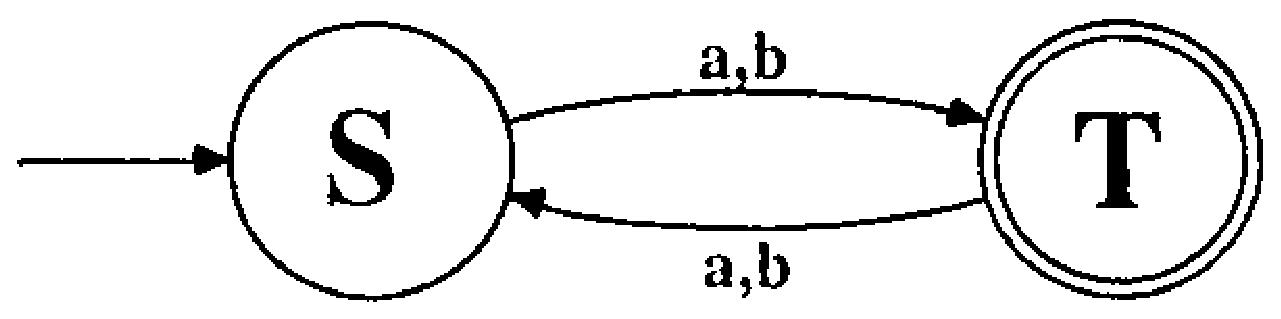
\epsfig{figure=ToFAfigures/fig8-1.eps,width=3in}}
\caption{The automaton discussed in Example 8.10}\label{fig-8.1}
\end{figure}

Lemma \ref{lmm-8.1} showed that a cognitive representation of a finite automaton definable
language can be expressed in an appropriate generative form (via a right-linear
grammar). There are many practical applications in which it is necessary to test
whether certain strings can be generated by a particular grammar. For
unrestricted grammars, the answers to such questions can be far from obvious. In
contrast, the specialized right-linear grammars discussed in this section can
always be transformed into a simple cognitive representation: every right-linear
grammar has a corresponding equivalent NDFA.

% Lemma 8.2
\begin{lmm}\label{lmm-8.2}
Let $\Sigma$ be any alphabet and $G=\langle\Omega,\Sigma,S,P\rangle$ be a
right-linear grammar, then there exists an NDFA $A_G$ (with $\lambda$-transitions)
for which $L(G)=L(A_G)$.

\emph{Proof.} Define $A_G=\langle\Sigma,Q_G,q_{0_G},\delta_G,F_G\rangle$, where
\begin{center}\begin{tabular}{r@{ }l}
$Q_G =$ & $\{\langle z\rangle\ |\ z=\lambda\vee z\in\Omega\vee\exists y\in
		\Sigma^*$ and $\exists B\in\Omega$ \\
& such that $B\rightarrow yz$ is a production in $P\}$ \\
$q_{0_G} =$ & $\{\langle S\rangle\}$ \\
$F_G =$ & $\{\langle\lambda\rangle\}$,
\end{tabular}\end{center}
and $\delta_G$ is comprised of (normal) transitions of the form
\begin{center}\begin{tabular}{r@{ }l}
$\delta_G(\langle w\rangle,\pmb{a}) =$ & $\{\langle x\rangle\ |\ \exists y\in(\Omega
	\cup\Sigma)^*,\exists B\in\Omega\ni w=\pmb{a}x \wedge B\rightarrow yw$ \\
& is a production in $P\}$
\end{tabular}\end{center}
$\delta_G$ also contains some $\lambda$-transitions of the form
\[ \delta_G(\langle B\rangle,\lambda)=\{\langle v\rangle\ |\ B\rightarrow v\text{ is
	a production in }P\} \]
As in the proof of Lemma \ref{lmm-8.1}, there is a one-to-one correspondence between paths
through the machine and derivations in the grammar. Inductive statements will be
the basis from which it will follow that $L(A_G)=L(G)$ (see the exercises).
\end{lmm}

The following example may be helpful in providing a firmer grasp of the
nature of $A_G$.

\subsection*{Example 8.11}

Let $G_1=\langle\{T,S\},\{\pmb{a},\pmb{b}\},S,\{S\rightarrow\pmb{a}S,S\rightarrow
\pmb{b}T,T\rightarrow\pmb{aa}\}\rangle$. Then
\[ A_{G_1}=\langle\{\pmb{a},\pmb{b}\},\{\langle\pmb{a}S\rangle,\langle S\rangle,
	\langle\pmb{b}T\rangle,\langle T\rangle,\langle\pmb{aa}\rangle,\langle
	\pmb{a}\rangle,\langle\lambda\rangle\},\{\langle S\rangle\},\delta_{G_1},
	\{\langle\lambda\rangle\}\rangle, \]
where $\delta_{G_1}$ is given by
\begin{center}\begin{tabular}{r@{ = }l@{$\qquad$}r@{ = }l}
$\delta_{G_1}(\langle S\rangle,\lambda)$ & $\{\langle\pmb{a}S\rangle,\langle
	\pmb{b}T\rangle\}$ & $\delta_{G_1}(\langle T\rangle,\lambda)$ &
	$\{\langle\pmb{aa}\rangle\}$ \\
$\delta_{G_1}(\langle\pmb{a}S\rangle,\pmb{a})$ & $\{\langle S\rangle\}$ &
	$\delta_{G_1}(\langle\pmb{b}T\rangle,\pmb{b})$ & $\{\langle T\rangle\}$ \\
$\delta_{G_1}(\langle\pmb{aa}\rangle,\pmb{a})$ & $\{\langle\pmb{a}\rangle\}$ &
	$\delta_{G_1}(\langle\pmb{a}\rangle,\pmb{a})$ & $\{\langle\lambda\rangle\}$
\end{tabular}\end{center}
and all other transitions are empty [for example, $\delta_{G_1}(\langle S\rangle,
\pmb{a}) = \emptyset$]. This automaton is shown in Figure \ref{fig-8.2}. Note that
$\pmb{abaa}$ is accepted by this machine by visiting the states $\langle S\rangle,\ 
\langle\pmb{a}S\rangle,\ \langle S\rangle,\ \langle\pmb{b}T\rangle,\ \langle T
\rangle,\ \langle\pmb{aa}\rangle,\ \langle\pmb{a}\rangle,\ \langle\lambda\rangle$,
and that the corresponding derivation in $G_1$ is $S\Rightarrow\pmb{a}S
\Rightarrow\pmb{ab}T\Rightarrow\pmb{abaa}$.

% Figure 8.2
\begin{figure}
\centerline{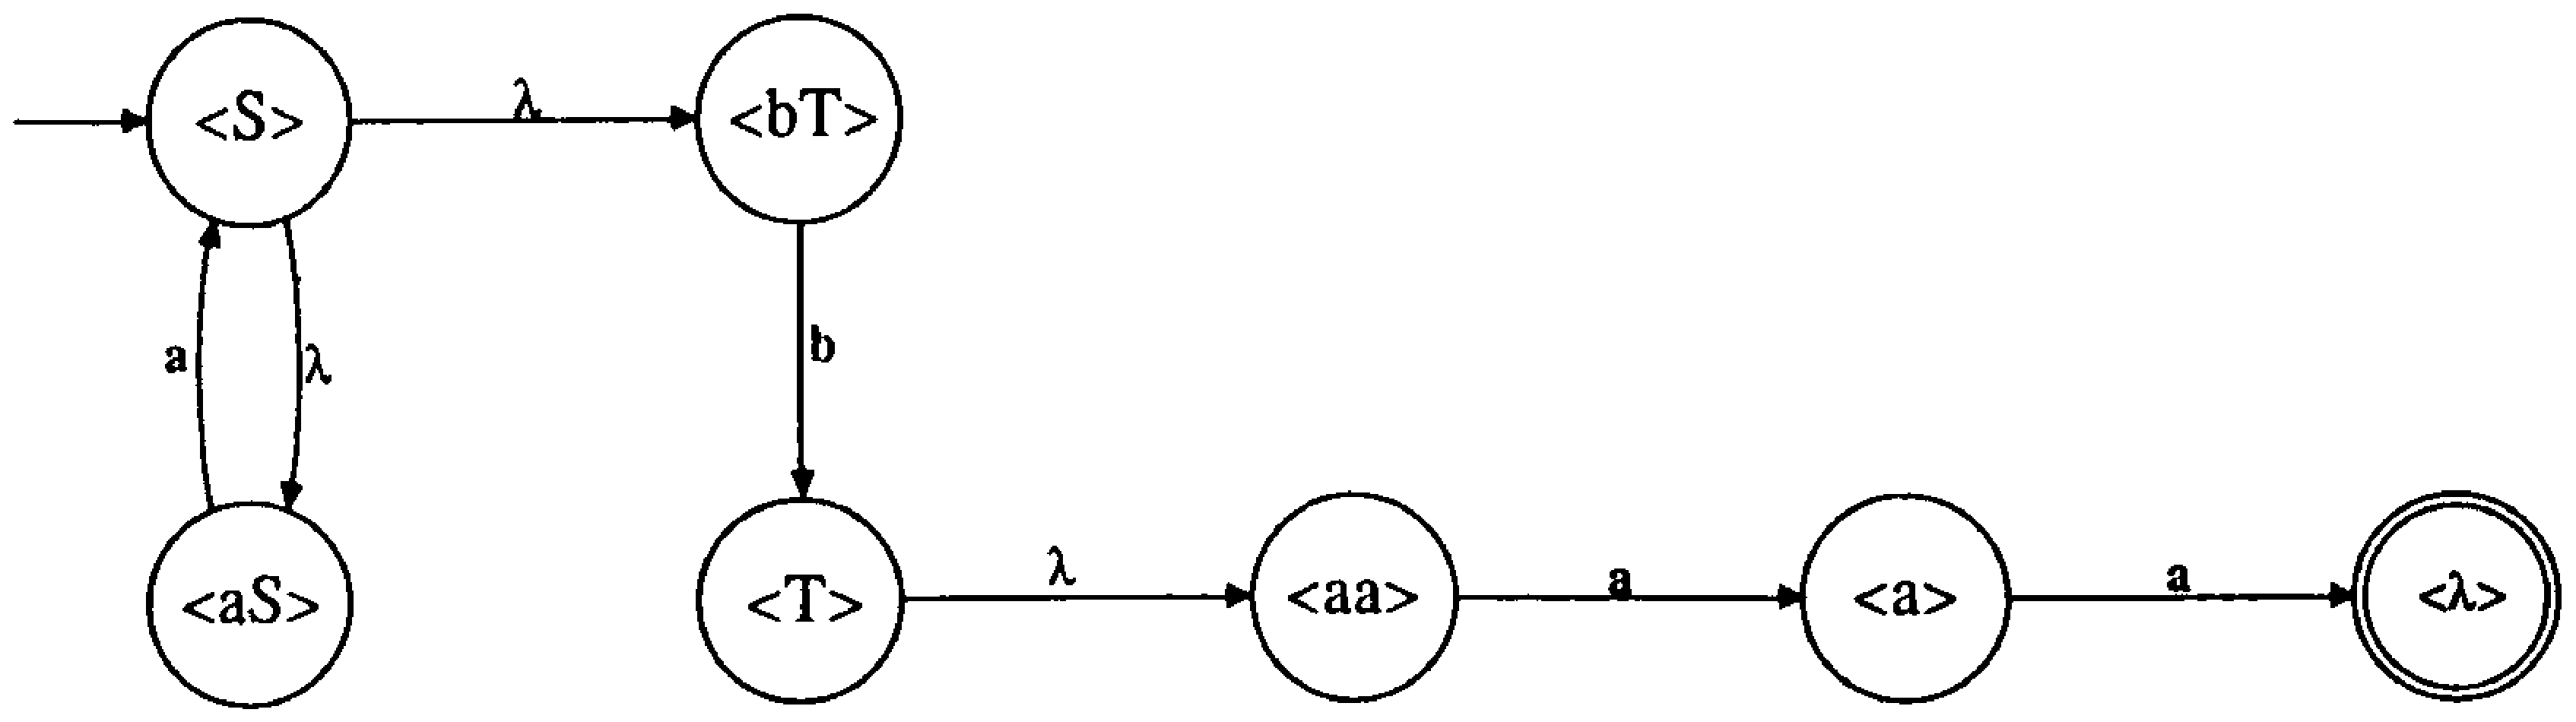
\epsfig{figure=ToFAfigures/fig8-2.eps,width=6.2in}}
\caption{The automaton corresponding to the grammar $G_1$}\label{fig-8.2}
\end{figure}

% Theorem 8.1
\begin{thm}\label{thm-8.1}
Given any alphabet $\Sigma$, $\GSIG = \DSIG$.

\emph{Proof.} Lemma \ref{lmm-8.1} guaranteed that every DFA has a corresponding grammar,
and so $\DSIG\subseteq\GSIG$. By Lemma \ref{lmm-8.2}, every grammar has a corresponding
NDFA, and so $\GSIG\subseteq\WSIG=\DSIG$. Thus $\GSIG=\DSIG$.
\end{thm}

\section{Regular Grammars and Regular Expressions}\label{sec-8.3}

The grammars we have considered so far are called \emph{right} linear because
productions are constrained to have the resulting nonterminal appear to the
right of the terminal symbols. We next consider the class of grammars that
arises by forcing the lone nonterminal to appear to the left of the terminal
symbols.

% Definition 8.11
\begin{dfn}\label{dfn-8.11}\index{language!type $k$}
A \emph{\Index{left-linear grammar}} over an alphabet $\Sigma$ is a quadruple
$G=\langle\Omega,\Sigma,S,P\rangle$, where:

\begin{quote}
$\Omega$ is a (nonempty) set of \emph{nonterminals}. \\
$\Sigma$ is a (nonempty) set of \emph{terminal symbols} (and $\Omega\cap\Sigma =
	\emptyset$). \\
$S$ is the designated \emph{start symbol} (and $S\in\Omega$). \\
$P$ is a set of \emph{productions} of the form $A\rightarrow Bx$, where $A\in\Omega,B
	\in(\Omega\cup\lambda)$, and $x\in\Sigma^*$.
\end{quote}
\end{dfn}
Note that a typical production might now look like $A\rightarrow B\pmb{cd}$,
where the nonterminal $B$ occurs to the left of the terminal string $\pmb{cd}$.

\subsection*{Example 8.12}

Let $G_2=\langle\{A,S\},\{\pmb{a},\pmb{b}\},S,\{S\rightarrow A\pmb{baa},A
\rightarrow A\pmb{a},A\rightarrow \lambda\}\rangle$. Then
\[ L(G_2)=\pmb{a}^*\pmb{baa}=\{\pmb{baa},\pmb{abaa},\pmb{aabaa},\ldots\} =
	L(G_1), \]
and so $G_2 \simeq G_1$ (compare with Example 8.7). Note that there does not
seem to be an obvious way to transform the right-linear grammar $G_1$ discussed
in Example 8.7 into an equivalent left-linear grammar such as $G_2$ (see the
exercises).

As was done for right-linear grammars in the last section, we \emph{could} show
that these left-linear grammars also generate the set of regular languages by
constructing corresponding machines and grammars (see the exercises). However,
we will instead prove that left-linear grammars are equivalent in power to
right-linear grammars by applying known results from previous chapters. The key
to this strategy is the reverse operator $r$ (compare with Example 4.10 and
Exercises 5.20 and 6.36).

% Definition 8.12
\begin{dfn}\label{dfn-8.12}
For an alphabet $\Sigma$, and $x=\pmb{a}_1\pmb{a}_2\cdots\pmb{a}_{n-1}\pmb{a}_n
\in\Sigma^*$; define $x^r=\pmb{a}_n\pmb{a}_{n-1}\cdots\pmb{a}_2\pmb{a}_1$. For a
language $L$ over $\Sigma$, define $L^r=\{x^r\ |\ x\in L\}$. For a grammar $G =
\langle\Omega,\Sigma,S,P\rangle$, define $G^r=\langle\Omega,\Sigma,S,P'\rangle$,
where $P'$ is given by $P'=\{A\rightarrow x^r\ |\ A\rightarrow x$ was a production
in $P\}$.
\end{dfn}

% Lemma 8.3
\begin{lmm}\label{lmm-8.3}
Let $G$ be a right-linear grammar. Then $G^r$ is a left-linear grammar, and
$L(G^r) = L(G)^r$. Similarly, if $G$ is a left-linear grammar, then $G^r$ is a
right-linear grammar, and again $L(G^r) = L(G)^r$.

\emph{Proof.} A straightforward induction on the number of productions used to
produce a given terminal string (see the exercises). It can be shown that $S 
\,\DRightarrow Bx$ by applying $n$ productions from $G$ iff $S\,\DRightarrow x^rB$
by applying $n$ corresponding productions from $G^r$.
\end{lmm}

\subsection*{Example 8.13}

Consider
\[ G_3=\langle\{T,S\},\{\pmb{a},\pmb{b},\pmb{c},\pmb{d}\},S,\{S\rightarrow
	\pmb{ab}S,S\rightarrow\pmb{cd}T,T\rightarrow\pmb{b}T,T\rightarrow
	\pmb{b}\}\rangle. \]
Then
\begin{center}\begin{tabular}{r@{ = }l}
$G_3^r$ & $\langle\{T, S\},\{\pmb{a},\pmb{b},\pmb{c},\pmb{d}\},S,\{S\rightarrow
	S\pmb{ba},S\rightarrow T\pmb{dc},T\rightarrow T\pmb{b},T\rightarrow
	\pmb{b}\}\rangle$, \\
$L(G_3)$ & $(\pmb{ab})^*\pmb{cdbb}^*$, $L(G^r_3)=\pmb{b}^*\pmb{bdc}(\pmb{ba})^*,$
\end{tabular}\end{center}
and
\[ L(G^r_3) = L(G_3)^r\ [\text{and }L(G_3) = L(G^r_3)^r]. \]

% Theorem 8.2
\begin{thm}\label{thm-8.2}
Let $\Sigma$ be an alphabet. Then the class of languages generated by the set of
all left-linear grammars over $\Sigma$ is the same as the class of languages
generated by the set of all right-linear grammars over $\Sigma$.

\emph{Proof.} Let $G$ be a left-linear grammar. $G^r$ is then a right-linear
grammar, and $L(G^r)$ is therefore FAD by Theorem \ref{thm-8.1}. Since \DSIG\ is closed
under the reverse operator $r$ (see Exercise 5.20), $L(G^r)^r$ is also FAD. But,
by Lemma \ref{lmm-8.3}, $L(G^r)^r = L(G)$, and so $L(G)$ is FAD. Hence every left-linear
grammar generates a member of \DSIG\ and therefore (by Lemma \ref{lmm-8.3}) has a corresponding
right-linear grammar.

Conversely, if $L$ is generated by a right-linear grammar, then $L$ is a
language in \DSIG, and so is $L^r$ (as shown by Exercise 5.20 or 6.36). Since
$\DSIG=\GSIG$, there is a right-linear grammar $G$ that generates $L^r$, and
hence $G^r$ is a left-linear grammar that generates $L$ (why?). Thus every
right-linear grammar has a corresponding left-linear grammar.
\end{thm}

% Definition 8.13
\begin{dfn}\label{dfn-8.13}\index{language!type $k$}
A \emph{regular} or \emph{\Index{type 3 grammar}} is a grammar that is either
right-linear or left-linear.
\end{dfn}
Thus, the languages generated by left-linear (and hence regular) grammars are
referred to as type 3 languages. The class of type 3 languages is exactly \GSIG.

% Corollary 8.1
\begin{cor}\label{cor-8.1}
The class of languages generated by regular grammars is equal to \GSIG.

\emph{Proof.} The proof follows immediately from Theorem \ref{thm-8.2}.
\end{cor}

With the correspondences developed between the grammatical descriptors and the
mechanical constructs, it is possible to transform a regular expression into
an equivalent grammar by first transforming the representation of the language
into an automaton (as described in Chapter \ref{ch-6}) and then applying Lemma \ref{lmm-8.1} to the
resulting machine. Conversely, the grammar $G_1$ in Example 8.11 gives rise to
the seven-state NDFA $A_{G_1}$ (using Lemma \ref{lmm-8.2}), which could in turn be used to
generate seven equations in seven unknowns. These could then be solved for a
regular expression representing $L(G_1)$ via Theorems \ref{thm-6.1} and \ref{thm-6.2}. A much more
efficient method, which generates equations directly from the productions
themselves, is outlined in the following theorem.

% Theorem 8.3
\begin{thm}\label{thm-8.3}
Let $G=\langle\{S_1,S_2,\ldots,S_n\},\Sigma,S_1,P\rangle$ be a right-linear
grammar, and for each nonterminal $S_i$ define $X_{s_i}$ to be the set of all
terminal strings that can be derived from $S_i$ by using the productions in $P$.
$X_{S_1}$ then represents $L(G)$, and these sets satisfy the language equations
\[ X_{S_k} = E_k\cup A_{k1}X_{S_1}\cup A_{k2}X_{S_2}\cup\cdots\cup A_{kn}X_{S_n},
	\qquad\text{ for }k = 1,2,\ldots,n \]
where $E_i$ is the union of all terminal strings $x$ that appear in productions
of the form $S_i\rightarrow x$, and $A_{ij}$ is the union of all terminal
strings $x$ that appear in productions of the form $S_i\rightarrow xS_j$.

\emph{Proof.} Since $S_1$ is the start symbol, $X_{S_1}$ is by definition the
set of all words that can be derived from the start symbol, and hence $X_{S_1} =
L(G)$. The relationships between the variables $X_{S_i}$ essentially embody the
relationships enforced by the productions in $P$.
\end{thm}

\subsection*{Example 8.14}

Consider $G_1$ from Example 8.11, in which
\[ G_1 = \langle\{T,S\},\{\pmb{a},\pmb{b}\},S,\{S\rightarrow\pmb{a}S,S\rightarrow
	\pmb{b}T,T\rightarrow\pmb{aa}\}\rangle. \]
The corresponding equations are
\begin{center}\begin{tabular}{r@{ = }l}
$X_S$ & $\emptyset\cup\pmb{a}X_S\cup\pmb{b}X_T$ \\
$X_T$ & $\pmb{aa}\cup\emptyset X_S\cup\emptyset X_T$
\end{tabular}\end{center}
Eliminating $X_T$ via Theorem \ref{thm-6.2} yields $X_S=\pmb{baa}\cup\pmb{a}X_S$. Theorem
\ref{thm-6.1} can be applied to this equation to yield $X_S=L(G_1)=\pmb{a}^*\pmb{baa}$.
Solving these two equations is indeed preferable to appealing the resulting NDFA
from Example 8.11 and solving the corresponding seven equations.

\subsection*{Example 8.15}

Let $\Sigma=\{\pmb{a},\pmb{b},\pmb{c}\}$, and consider the set of all words that
end in $\pmb{b}$ and for which every $\pmb{c}$ is immediately followed by $\pmb{a}$.
This can be succinctly described by the grammar $G=\langle\{S\},\{\pmb{a},
\pmb{b},\pmb{c}\},S,\{S\rightarrow\pmb{a}S,S\rightarrow\pmb{b}S,S\rightarrow
\pmb{ca}S,S\rightarrow\pmb{b}\}\rangle$. The resulting one equation in the
single unknown $X_S$ is $X_S=\pmb{b}\cup(\pmb{a}\cup\pmb{b}\cup\pmb{ca})X_S$,
and Theorem \ref{thm-6.1} can be applied to yield a regular expression for this language;
that is, $X_S=(\pmb{a}\cup\pmb{b}\cup\pmb{ca})^*\pmb{b}$.

Unfortunately, another grammar that generates this same language is
\[ G'=\langle\{S\},\{\pmb{a},\pmb{b},\pmb{c}\},S,\{S\rightarrow\lambda S,S
	\rightarrow\pmb{a}S,S\rightarrow\pmb{b}S,S\rightarrow\pmb{ca}S,S
	\rightarrow\pmb{b}\}\rangle. \]
In this case, however, the resulting one equation in the single unknown $X_S$ is
$X_S=\pmb{b}\cup(\lambda\cup\pmb{a}\cup\pmb{b}\cup\pmb{ca})X_S$, and Theorem \ref{thm-6.1}
explicitly prohibits $\lambda$ from appearing as a coefficient of an unknown.
The equation no longer has a unique solution; other solutions are now possible,
such as $X_S=\Sigma^*$. Nevertheless, the reduction described by Theorem \ref{thm-6.1}
still predicts the correct expression for this language; that is, $X_S=(\lambda
\cup\pmb{a}\cup\pmb{b}\cup\pmb{ca})^*\pmb{b}$. For equations arising from
grammatical constructs, the desired solution will \emph{always} be the minimal
solution predicted by the technique used in Theorem \ref{thm-6.1}. The condition
prohibiting $\lambda$ from appearing in the set $A$ in the equation $X=E\cup AX$
was required to guarantee a unique solution. Regardless of the nature of the set
$A$, $A^*E$ is guaranteed to be a solution, and it will be contained in any
other solution, as restated in Lemma \ref{lmm-8.4}.

% Lemma 8.4
\begin{lmm}\label{lmm-8.4}
Let $E$ and $A$ be any two sets, and consider the language equation $X=E\cup AX$.
$A^*E$ is always a solution for $X$, and any other solution $Y$ must satisfy the
property $A^*E \subseteq Y$.

\emph{Proof.} Follows immediately from Theorem \ref{thm-6.1}.
\end{lmm}

Consider again the grammar
\[ G' = \langle\{S\},\{\pmb{a},\pmb{b},\pmb{c}\},S,\{S\rightarrow\lambda S,S
	\rightarrow\pmb{a}S,S\rightarrow\pmb{b}S,S\rightarrow\pmb{ca}S,S
	\rightarrow\pmb{b}\}\rangle, \]
which generates the language $(\lambda\cup\pmb{a}\cup\pmb{b}\cup\pmb{ca})^*
\pmb{b}$. The corresponding equation was $X=E\cup AX$, where $E=\pmb{b}$, and
$A=(\lambda\cup\pmb{a}\cup\pmb{b}\cup\pmb{ca})$. Note that $E$ represents the
set of terminal strings that can be generated from $S$ using exactly one
production, while $A\cdot E=(\lambda\cup\pmb{a}\cup\pmb{b}\cup\pmb{ca})\pmb{b}$
is the set of all strings that can be generated from $S$ using exactly two
productions. Similarly, $A\cdot A\cdot E$ represents all terminal strings
that can be generated from $S$ using exactly three productions. By induction, it
can be shown that $A^{n-1}\cdot E$ is the set of all strings that can be
generated from S using exactly $n$ productions. From this it follows that the
minimal solution $A^*E$ is indeed the language generated by the grammar.

Clearly, a useless production of the form $S\rightarrow\lambda S$ in a grammar
can simply be removed from the production set without affecting the language
that is generated. In the above example, it was the production $S\rightarrow
\lambda S$ that was responsible for $\lambda$ appearing in the coefficient set
$A$. It is only the \emph{nongenerative} productions, which do not produce any
terminal symbols, that can give rise to a nonunique solution. However, the
removal of productions of the form $V\rightarrow\lambda T$ will require the
addition of other productions when $T$ is a different nonterminal than $V$.
Theorem \ref{thm-9.4}, developed later, will show that these grammars can be transformed
into equivalent grammars that do not contain productions of the form $V
\rightarrow\lambda T$. Theorem \ref{thm-8.4} shows that it is not necessary to perform
such transformations before producing equations that will provide equivalent
regular expressions: the techniques outlined in Theorem \ref{thm-6.2} can indeed be used
to solve systems of equations, even if the coefficients contain the empty word.
Indeed, the minimal solution found in this manner will be the regular expression
sought. This robustness is similar to that found in Theorem \ref{thm-6.3}, which was
stated for deterministic finite automata. Regular expressions for
nondeterministic finite automata can be generated by transforming the NDFA into
a DFA and then applying Theorem \ref{thm-6.3}, but it was seen that it is both possible
and more efficient to apply the method directly to the NDFA without performing
the transformation. The following theorem justifies that a transformation to a
well-behaved grammar is an unnecessary step in the algorithm for finding a
regular expression describing the language generated by a right-linear grammar.

% Lemma 8.5
\begin{lmm}\label{lmm-8.5}
Consider the system of equations in the unknowns $X_1,X_2,\ldots,X_n$ given by
\begin{center}\begin{tabular}{r@{ }c@{ }l}
$X_1$ & $=$ & $E_1\cup A_{11}X_1\cup A_{12}X_2\cup\cdots\cup A_{1(n-1)}X_{n-1}
	\cup A_{1n}X_n$ \\
$X_2$ & $=$ & $E_2\cup A_{21}X_{1}\cup A_{22}X_2\cup\cdots\cup A_{2(n-1)}X_{n-1}
	\cup A_{2n}X_n$ \\
& $\cdot$ \\
& $\cdot$ \\
& $\cdot$ \\
$X_{n-1}$ & $=$ & $E_{n-1}\cup A_{(n-1)1}X_1\cup A_{(n-1)2}X_2\cup\cdots\cup
	A_{(n-1)(n-1)}X_{n-1}\cup A_{(n-1)n}X_n$ \\
$X_n$ & $=$ & $E_n\cup A_{n1}X_1\cup A_{n2}X_2\cup\cdots\cup A_{n(n-1)}X_{n-1}
	\cup A_{nn}X_n$
\end{tabular}\end{center}
\begin{enumerate}[a.]
\item Define $\hat{E}_i = E_i\cup (A_{in}\cdot A^*_{nn}\cdot E_n)$ for all $i =
1,2,\ldots,n-1$ and
\[ \hat{A}_{ij}=A_{ij}\cup(A_{in}\cdot A^*_{nn}\cdot A_{nj})\text{ for all }i,j
	= 1,2,\ldots,n-1. \]
Any solution of the original set of equations will agree with a solution of
the following set of $n-1$ equations in the unknowns $X_1,X_2,\ldots,X_{n-1}$:
\begin{center}\begin{tabular}{r@{ }c@{ }l}
$X_1$ & $=$ & $\hat{E}_1\cup \hat{A}_{11}X_1\cup\hat{A}_{12}X_2\cup\cdots\cup
	\hat{A}_{1(n-1)}X_{n-1}$ \\
$X_2$ & $=$ & $\hat{E}_2\cup \hat{A}_{21}X_{1}\cup\hat{A}_{22}X_2\cup\cdots\cup
	\hat{A}_{2(n-1)}X_{n-1}$ \\
& $\cdot$ \\
& $\cdot$ \\
& $\cdot$ \\
$X_{n-1}$ & $=$ & $\hat{E}_{n-1}\cup \hat{A}_{(n-1)1}X_1\cup\hat{A}_{(n-1)2}X_2
	\cup\cdots\cup\hat{A}_{(n-1)(n-1)}X_{n-1}$
\end{tabular}\end{center}

\item Given a solution to the above $n-1$ equations in (a), that solution can be
used to find a compatible expression for the remaining unknown:
\[ X_n=A^*_{nn}\cdot(E_n\cup A_{n1}X_1\cup A_{n2}X_2\cup\cdots\cup A_{n(n-1)}
	X_{n-1}) \]

\item This system has a unique \emph{minimal} solution in the following sense:
Let $W_1,W_2,\ldots,W_n$ denote the solution found by eliminating variables and
back-substituting as specified in (a) and (b). If $Y_1,Y_2,\ldots,Y_n$ is any
other solution to the original $n$ equations in $n$ unknowns, then $W_1\subseteq
Y_1,W_2\subseteq Y_2,\ldots$, and $W_n\subseteq Y_n$.
\end{enumerate}

\emph{Proof.} This proof is by induction on the number of equations. Lemma \ref{lmm-8.4}
proved the basis step for $n=1$. As in Theorem \ref{thm-6.2}, the inductive step is proved
by considering the last of the $n$ equations,
\[ X_n = (E_n\cup A_{n1}X_1\cup A_{n2}X_2\cup\cdots\cup A_{n(n-1)}X_{n-1})\cup
	A_{nn}X_n \]
This can be thought of as an equation in the one unknown $X_n$ with a coefficient
of $A_{nn}$ for $X_n$, and the remainder of the expression a ``constant'' term
not involving $X_n$.

For a given solution for $X_1$ through $X_{n-1}$ Lemma \ref{lmm-8.4} can therefore be
applied to the above equation in the one unknown $X_n$, with coefficients
\[ E = (E_n\cup A_{n1}X_1\cup A_{n2}X_2\cup\cdots\cup A_{n(n-1)}X_{n-1}) \]
and $A=A_{nn}$ to find a minimal solution for $X_n$ for the corresponding values of
$X_1$ through $X_{n-1}$. This is exactly as given by part (b) above:
\[ X_n=A^*_{nn}\cdot(E_n\cup A_{n1}X_1\cup A_{n2}X_2\cup\cdots\cup A_{n(n-1)}
	X_{n-1}) \]
or
\[ X_n = A^*_{nn}\cdot E_n\cup A^*_{nn}\cdot A_{n1}X_1\cup A^*_{nn}\cdot A_{n2}
	X_2\cup\cdots\cup A^*_{nn}\cdot A_{n(n-1)}X_{n-1}) \]
Specifically, if $X_1$ through $X_{n-1}$ are represented by a minimal solution
$W_1$ through $W_{n-1}$, then Lemma \ref{lmm-8.4} implies that the inclusion of $W_n$,
given by
\[ W_n = A^*_{nn}\cdot E_n\cup A^*_{nn}\cdot A_{n1}W_1\cup A^*_{nn}\cdot A_{n2}
	W_2\cup\cdots\cup A^*_{nn}\cdot A_{n(n-1)}W_{n-1} \]
will yield a minimal solution $W_1$ through $W_n$ of the original $n$ equations
in $n$ unknowns.

The minimal solution for the $n-1$ equations in the unknowns $X_1,X_2,\ldots,
X_{n-1}$, denoted by $W_1$ through $W_{n-1}$ can be found by substituting this
particular solution $W_n$ for $X_n$ in each of the other $n-1$ equations. If the
$k^{th}$ equation is represented by
\[ X_k = E_k\cup A_{k1}X_1\cup A_{k2}X_2\cup\cdots\cup A_{kn}X_n \]
then the substitution will yield
\begin{center}\begin{tabular}{r@{ }l}
$X_k =$ & $E_k\cup A_{k1}X_1\cup A_{k2}X_2\cup\cdots$ \\
& $\cup\ (A_{kn}\cdot(A^*_{nn}\cdot E_n\cup A^*_{nn}\cdot A_{n1}X_1\cup A^*_{nn}
	\cdot A_{n2}X_2\cup\cdots\cup A^*_{nn}\cdot A_{n(n-1)}X_{n-1}))$
\end{tabular}\end{center}
Due to the nature of union and concatenation, no other solution for $X_n$ can
possibly allow a smaller solution for $X_1,X_2,\ldots,X_{n-1}$ to be found.
Specifically, if $Y_n$ is a solution satisfying the $n^{th}$ equation, then Lemma
\ref{lmm-8.4} guarantees that $W_n \subseteq Y_n$, and consequently
\[ X_k = E_k\cup A_{k1}X_1\cup A_{k2}X_2\cup\cdots\cup A_{kn}W_n \subseteq E_k
	\cup A_{k1}X_1\cup A_{k2}X_2\cup\cdots\cup A_{kn}Y_n \]
Thus, the minimal value for each $X_k$ is compatible with the substitution of
$W_n$ defined earlier. Hence, by using the distributive law, the revised
equation becomes
\begin{center}\begin{tabular}{r@{ }l}
$X_k =$ & $E_k\cup A_{k1}X_1\cup A_{k2}X_2\cup\cdots\cup(A_{kn}\cdot A^*_{nn}\cdot
	E_n\cup A_{kn}\cdot A^*_{nn}\cdot A_{n1}X_1$ \\
& $\cup\ A_{kn}\cdot A^*_{nn}\cdot A_{n2}X_2\cup\cdots\cup A_{kn}\cdot A^*_{nn}
	\cdot A_{n(n-1)}X_{n-1})$
\end{tabular}\end{center}
Collecting like terms yields
\begin{center}\begin{tabular}{r@{ }l}
$X_k =$ & $(E_k\cup A_{kn}\cdot A^*_{nn}\cdot E_n)\cup(A_{k1}X_1\cup A_{kn}\cdot
	A^*_{nn}\cdot A_{n1}X_1)$ \\
& $\cup\ (A_{k2}X_2\cup A_{kn}\cdot A^*_{nn}\cdot A_{n2}X_2)\cup\cdots\cup
	(A_{k(n-1)}X_{n-1}\cup A_{kn}\cdot A^*_{nn}\cdot A_{n(n-1)}X_{n-1})$,
\end{tabular}\end{center}
or
\begin{center}\begin{tabular}{r@{ }l}
$X_k =$ & $(E_k\cup A_{kn}\cdot A^*_{nn}\cdot E_n)\cup(A_{k1}\cup A_{kn}\cdot
	A^*_{nn}\cdot A_{n1})X_1$ \\
& $\cup\ (A_{k2}\cup A_{kn}\cdot A^*_{nn}\cdot A_{n2})X_2\cup\cdots\cup(A_{k(n-1
	)}\cup A_{kn}\cdot A^*_{nn}\cdot A_{n(n-1)})X_{n-1}$
\end{tabular}\end{center}
The constant term in this equation is $(E_k\cup A_{kn}\cdot A^*_{nn}\cdot E_n)$,
and the coefficient for $X_j$ is $\hat{A}_{kj} = A_{kj}\cup(A_{kn}\cdot A^*_{nn}
\cdot A_{nj})$, which agrees with the formula given in (a). The substitution of
$X_n$ was shown to yield a minimal set of $n-1$ equations in the unknowns $X_1$
through $X_{n-1}$, and the induction assumption guarantees that the elimination
and back-substitution method yields a minimal solution for $W_1$ through
$W_{n-1}$. Lemma \ref{lmm-8.4} then guarantees that the solution for
\[ W_n = A^*_{nn}\cdot E_n\cup A^*_{nn}\cdot A_{n1}W_1\cup A^*_{nn}\cdot A_{n2}
	W_2\cup\cdots\cup A^*_{nn}\cdot A_{n(n-1)}W_{n-1} \]
is minimal, which completes the minimal solution for the original system of $n$
equations.
\end{lmm}

As with Lemma \ref{lmm-8.4}, the minimal expressions thus generated describe exactly
those terminal strings that can be produced by a right-linear grammar. In an
analogous fashion, left-linear grammars give rise to a set of left-linear
equations, which can be solved as indicated in Theorem \ref{thm-6.4}.

The above discussion describes the transformation of regular grammars into
regular expressions. Generating grammars from regular expressions hinges on
the interpretation of the six building blocks of regular expressions, as
described in Definition \ref{dfn-6.2}. Since \GSIG\ is the same as \DSIG,\ all the closure
properties known about \DSIG\ must also apply to \GSIG, but it can be
instructive to reprove these theorems using grammatical constructions. Such
proofs will also provide guidelines for directly transforming a regular
expression into a grammar without first constructing a corresponding automaton.

% Theorem 8.4
\begin{thm}\label{thm-8.4}
Let $\Sigma$ be an alphabet. Then \GSIG\ is effectively closed under union.

\emph{Proof.} Let $G_1=\langle\Omega_1,\Sigma,S_1,P_1\rangle$ and $G_2=\langle
\Omega_2,\Sigma,S_2,P_2\rangle$ be two right-linear grammars, and without loss
of generality assume that $\Omega_1\cap\Omega_2=\emptyset$. Choose a new
nonterminal $Z$ such that $Z \notin \Omega_1\cup\Omega_2$, and consider the new
grammar $G^{\cup}$ defined by $G^{\cup}=\langle\Omega_1\cup\Omega_2\cup\{Z\},
\Sigma,Z,P_1\cup P_2\cup\{Z\rightarrow S_1,Z\rightarrow S_2\}\rangle$. It is
straightforward to show that $L(G^{\cup})=L(G_1)\cup L(G_2)$ (see the exercises).
From the start symbol $Z$ there are only two productions that can be applied; if
$Z\rightarrow S_1$ is chosen, then the derivation will have to continue with
productions from $P_1$ and produce a word from $L(G_1)$ (why can't productions
from $P_2$ be applied?). Similarly, if $Z\rightarrow S_2$ is chosen instead, the
only result can be a word from $L(G_2)$.
\end{thm}

In an analogous fashion, effective closure of \GSIG\ can be demonstrated for the
operators Kleene closure and concatenation. The proof for Kleene closure is
outlined below. The construction for concatenation is left for the exercises;
the technique is illustrated in Example 8.18.

% Theorem 8.5
\begin{thm}\label{thm-8.5}
Let $\Sigma$ be an alphabet. Then \GSIG\ is effectively closed under
\Index{Kleene closure}.

\emph{Proof.} Let $G=\langle\Omega,\Sigma,S,P\rangle$ be a right-linear grammar.
Choose a new nonterminal $Z$ such that $Z \notin \Omega$, and consider the new
grammar $G_*$ defined by
\[ G_* = \langle\Omega\cup\{Z\},\Sigma,Z,P_*\rangle, \]
where
\begin{center}\begin{tabular}{r@{ }l}
$P_* =$ & $\langle\{Z\rightarrow\lambda,Z\rightarrow S\}$ \\
& $\cup\{A\rightarrow xB\ |\ (x\in\Sigma^*)\wedge(A,B\in\Omega)\wedge(A\rightarrow
	xB\in P)\}$ \\
& $\cup\{A\rightarrow xZ\ |\ (x\in\Sigma^*)\wedge(A\in\Omega)\wedge(A\rightarrow x
	\in P)\}\rangle$.
\end{tabular}\end{center}
That is, all productions in $P$ that end in a nonterminal are retained, while
all other productions in $P$ are appended with the new symbol $Z$, and the two
new productions $Z\rightarrow\lambda$ and $Z\rightarrow S$ are added. A
straightforward induction argument will show that the derivations that use $n$
applications of productions of the form $A\rightarrow xZ$ generate exactly the
words in $L(G)^n$. Consequently, $L(G_*) = L(G)^*$.
\end{thm}

% Theorem 8.6
\begin{thm}\label{thm-8.6}
Let $\Sigma$ be an alphabet. Then \GSIG\ is effectively closed under
concatenation.

\emph{Proof.} See the exercises.
\end{thm}

% Corollary 8.2
\begin{cor}\label{cor-8.2}
Every regular expression has a corresponding right-linear grammar.

\emph{Proof.} While this follows immediately from the fact that $\GSIG=\DSIG$
and Theorem \ref{thm-6.1}, the previous theorems outline an effective procedure for
transforming a regular expression into a right-linear grammar. This can be
proved by induction on the number of operators in the regular expression. The
basis step consists of the observation that expressions with zero operators,
which must be of the form $\emptyset,\ \lambda$, or $\pmb{a}$, can be represented
by the right-linear grammars $\langle\{S\},\Sigma,S,\{S\rightarrow S\}\rangle$,
$\langle\{S\},\Sigma,S,\{S\rightarrow\lambda\}\rangle$, and $\langle\{S\},\Sigma,
S,\{S\rightarrow\pmb{a}\}\rangle$, respectively.

To prove the inductive step, choose an arbitrary regular expression $R$ with
$m+1$ operators, and identify the outermost operator. $R$ must be of the form
$R_1\cup R_2$ or $R_1\cdot R_2$ or $R^*_1$, where $R_1$ (and $R_2$) have $m$ or
fewer operators. By the induction hypothesis, $R_1$ (and $R_2$) can be
represented as right-linear grammars, and therefore by Theorem \ref{thm-8.4}, \ref{thm-8.5}, or \ref{thm-8.6},
$R$ can also be represented by a right-linear grammar. Any regular expression
can thus be methodically transformed into an equivalent right-linear grammar.
\end{cor}

\subsection*{Example 8.16}

Let $\Sigma=\{\pmb{a},\pmb{b},\pmb{c}\}$, and consider the regular expression
$(\pmb{a}\cup\pmb{b})$. The grammars $G_1=\langle\{R\},\{\pmb{a},\pmb{b},\pmb{c}
\},R,\{R\rightarrow\pmb{a}\}\rangle$ and $G_2=\langle\{T\},\{\pmb{a},\pmb{b},
\pmb{c}\},T,\{T\rightarrow\pmb{b}\}\rangle$ can be combined as suggested in
Theorem \ref{thm-8.4} (with $A$ playing the role of $Z$) to form $G=\langle\{T,R,A\},\{
\pmb{a},\pmb{b},\pmb{c}\},A,\{A\rightarrow R,A\rightarrow T,R\rightarrow\pmb{a},
T\rightarrow\pmb{b}\}\rangle$.

\subsection*{Example 8.17}

Consider the regular expression $(\pmb{a}\cup\pmb{b})^*$. The grammar
\[ G=\langle\{T,R,A\},\{\pmb{a},\pmb{b},\pmb{c}\},A,\{A\rightarrow R,A
	\rightarrow T,R\rightarrow\pmb{a},T\rightarrow\pmb{b}\}\rangle \]
from Example 8.16 can be modified as suggested in Theorem \ref{thm-8.5} to form
\[ G_* = \langle\{T,R,A,Z\},\{\pmb{a},\pmb{b},\pmb{c}\},Z,\{Z\rightarrow\lambda,
	Z\rightarrow A,A\rightarrow R,A\rightarrow T,R\rightarrow\pmb{a}Z,T
	\rightarrow\pmb{b}Z\}\rangle. \]
$G_*$ generates $(\pmb{a}\cup\pmb{b})^*$.

\subsection*{Example 8.18}

Consider the regular expression $(\pmb{a}\cup\pmb{b})^*\pmb{c}$. The grammars
\[ G_* = \langle\{T,R,A,Z\},\{\pmb{a},\pmb{b},\pmb{c}\},Z,\{Z\rightarrow\lambda,
	Z\rightarrow A,A\rightarrow R,A\rightarrow T,R\rightarrow\pmb{a}Z,T
	\rightarrow\pmb{b}Z\}\rangle. \]
and
\[ G_3 = \langle\{V\},\{\pmb{a},\pmb{b},\pmb{c}\},V,\{V\rightarrow\pmb{c}\}
	\rangle \]
can be combined with modified productions to form
\begin{center}\begin{tabular}{r@{ }l}
$G' =$ & $\langle\{T,R,A,Z,V,S\},\{\pmb{a},\pmb{b},\pmb{c}\},S,$ \\
& $\{S\rightarrow Z,Z\rightarrow \lambda V,Z\rightarrow A,A\rightarrow R,A
	\rightarrow T,R\rightarrow\pmb{a}Z,T\rightarrow\pmb{b}Z,V\rightarrow
	\pmb{c}\}\rangle$.
\end{tabular}\end{center}
$G'$ generates $(\pmb{a}\cup\pmb{b})^*\pmb{c}$.

The previous examples illustrate the manner in which regular expressions can
be systematically translated into right-linear grammars. Constructions
corresponding to those given in Theorems \ref{thm-8.4}, \ref{thm-8.5}, and \ref{thm-8.6} can similarly be
found for left-linear grammars (see the exercises).

\emph{Normal forms} for grammars are quite useful in many contexts. A standard
representation can be especially useful in proving theorems about grammars. For
example, the construction given in Lemma \ref{lmm-8.2} would have been more concise and
easier to investigate if complex productions such as $S\rightarrow\pmb{bcaa}T$
could be avoided. Indeed, if all productions in the grammar $G$ had been of the
form $A\rightarrow\pmb{a}B$ or $A\rightarrow\lambda$, both the state set and the
state transition function of $A_G$ could have been defined more easily. Other
constructions and proofs may also be able to make use of the simpler types of
productions in grammars that conform to such normal forms. The following theorem
guarantees that a given right-linear grammar has a corresponding equivalent
grammar containing only productions that conform to the above standard.

% Theorem 8.7
\begin{thm}\label{thm-8.7}
Every right-linear grammar $G$ has an equivalent right-linear grammar $G^1$ in
which all productions are of the form $A\rightarrow\pmb{a}B$ or $A\rightarrow
\lambda$.

\emph{Proof.} Let $G$ be a right-linear grammar. By Lemma \ref{lmm-8.2}, there exists an
NDFA $A_G$ that is equivalent to $G$. From Chapter \ref{ch-4}, $A^d_G$ is an equivalent
deterministic finite automaton, and Lemma \ref{lmm-8.1} can be applied to $A^d_G$ to form
an equivalent right-linear grammar. By the construction given in Lemma \ref{lmm-8.1}, all
the productions in this grammar are indeed of the form $A\rightarrow\pmb{a}B$ or
$A\rightarrow\lambda$.
\end{thm}

Note that the proof given is a constructive proof: rather than simply arguing
the existence of such a grammar, a method for obtaining $G^1$ is outlined. The
above theorem could have been proved without relying on automata constructs.
Basically, ``long'' productions like $T\rightarrow\pmb{abc}R$ would be replaced
by a series of productions involving newly introduced nonterminals, for example,
$T\rightarrow\pmb{a}X,X\rightarrow\pmb{b}Y,Y\rightarrow\pmb{c}R$. Similarly, a
production like $T\rightarrow\pmb{aa}$ might be replaced by the sequence $T
\rightarrow\pmb{a}B,B\rightarrow\pmb{a}C,C\rightarrow\lambda$. If the existence
of such a normal form had been available for the proof of Lemma \ref{lmm-8.2}, the
construction of $A_G$ could have been simplified and the complexity of the proof
drastically curtailed. Indeed, the resulting machine would have contained no
$\lambda$-moves. Only one state per nonterminal would have been necessary, with
final states corresponding to nonterminals that had productions of the form $A
\rightarrow \lambda$. Productions of the form $A\rightarrow\pmb{a}B$ would imply
that $B\in\delta(A,\pmb{a})$.

\subsection*{Example 8.19}

$G = \langle\{S,T,B,C\},\{\pmb{a},\pmb{b}\},S,\{S\rightarrow\pmb{a}S,S
\rightarrow\pmb{b}T,T\rightarrow\pmb{a}B,B\rightarrow\pmb{a}C,C\rightarrow
\lambda\}\rangle$ can be represented by the NDFA shown in Figure \ref{fig-8.3}.

% Figure 8.3
\begin{figure}
\centerline{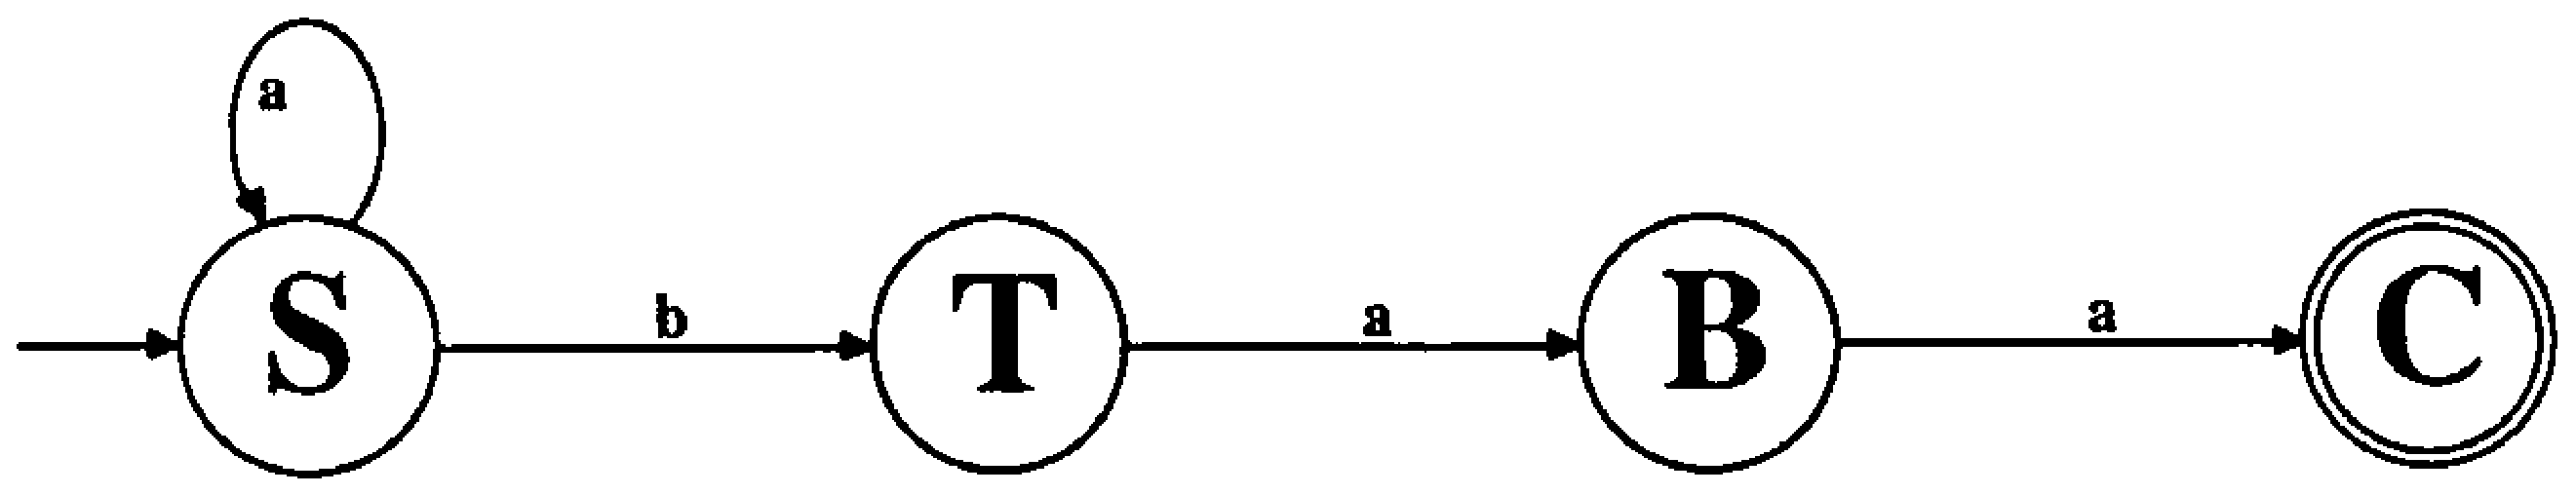
\epsfig{figure=ToFAfigures/fig8-3.eps,width=5.2in}}
\caption{An automaton corresponding to a grammar in normal form}\label{fig-8.3}
\end{figure}

In practice, given an arbitrary right-linear grammar $G$, the work associated
with finding the complex machine defined in Lemma \ref{lmm-8.2} has simply been replaced
by the effort needed to transform $G$ into the appropriate normal form.
Nevertheless, the guarantee that regular languages have grammars that conform to
the above normal form is useful in many proofs, as illustrated above and in
Theorem \ref{thm-8.8} below.

As with context-free and context-sensitive languages, the contracting
productions can be limited to $Z\rightarrow\lambda$, where $Z$ is the start
symbol. This is only necessary if $\lambda\in L$; if $\lambda\notin L$, there
need be no contracting productions at all. We wish to show how to produce a
right-linear grammar with no more than one contracting production. By relying on the
existence of the normal form described in Theorem \ref{thm-8.7}, this can be done without
dealing with right-linear grammars in their full generality.

% Theorem 8.8
\begin{thm}\label{thm-8.8}
Every right-linear grammar $G$ has an equivalent right-linear grammar $G^0$ in
which the start symbol $Z$ never appears on the right in any production, and the
only length-contracting production that may appear is $Z\rightarrow\lambda$.
Furthermore, all other productions are of the form $A\rightarrow\pmb{a}B$ or $A
\rightarrow\pmb{a}$.

\emph{Proof.} Let $G = \langle\Omega,\Sigma,S,P\rangle$ be a right-linear
grammar. Without loss of generality, assume that $G$ is of the form specified by
Theorem \ref{thm-8.7}. (If $G$ were not of the proper form, Theorem \ref{thm-8.7} guarantees that an
equivalent grammar that is in the proper form could be found and used in place
of $G$.) Choose a new nonterminal $Z$ such that $Z\notin\Omega$, and consider
the new grammar $G^0$ defined by $G^0 = \langle\Omega\cup\{Z\},\Sigma,Z,P^0
\rangle$, where $P^0$ contains $Z\rightarrow S$, and all productions from $P$
of the form $A\rightarrow xB$, where $x\in\Sigma^*$ and $A,B \in\Omega$. $P^0$
also contains the productions in the set $\{A\rightarrow\pmb{a}\ |\ (\exists B\in
\Omega)(A\rightarrow\pmb{a}B\in P \wedge B\rightarrow\lambda\in P)\}$. Finally,
if $S\rightarrow\lambda$ was a production in $P$, then $Z\rightarrow\lambda$ is
included in $P^0$. Note that no other productions of the form $B\rightarrow
\lambda$ are part of $P^0$. Other productions have been added to compensate for
this loss. Derivations using the productions in $P^0$ typically start with $Z
\rightarrow S$, then proceed with productions of the form $A\rightarrow xB$, and
terminate with one production of the form $A\rightarrow\pmb{a}$. The
corresponding derivation in the original grammar $G$ would be very similar, but
would start with the old start symbol $S$ and therefore avoid the $Z\rightarrow
S$ application used in $G^0$. The productions of the form $A\rightarrow xB$ are
common to both grammars, and the final step in $G^0$ that uses $A\rightarrow
\pmb{a}$ would be handled by two productions in $G$: $A\rightarrow\pmb{a}B$ and
$B\rightarrow\lambda$. An induction argument on the number of productions in a
derivation will show that every derivation from $G^0$ has a corresponding
derivation in $G$ that produces the same terminal string, and vice versa. Thus,
$L(G^0)=L(G)$, which justifies that $G^0$ is equivalent to $G$. $G^0$ was
constructed to conform to the conditions specified by the theorem, and thus the
proof is complete.
\end{thm}

% Corollary 8.3
\begin{cor}\label{cor-8.3}\index{hierarchy!of grammars}
Every type 3 language is also a type 2 language.

\emph{Proof.} Let $L$ be a type 3 language. Then there exists a right-linear
grammar $G$ that generates $L$. By Theorem \ref{thm-8.8}, there is an equivalent
right-linear grammar $G^0$ that satisfies the definition of a context-free
grammar. Thus, $L$ is context free.
\end{cor}

Section \ref{sec-8.1} explored several generalizations of the definition of a regular
grammar, and, unlike the generalization from DFAs to NDFAs, new and larger
classes of languages result from these generalizations. These new types of
grammars will be explored in the following chapters, and the corresponding
generalized machines will be developed.

\section*{Exercises}

\begin{enumerate}[{8.}1. ]
\item Can strings like $\pmb{ab}BA\pmb{d}B\pmb{c}$ (where $B$ and $A$ are nonterminals)
ever be derived from the start symbol $S$ in a right-linear grammar? Explain.

\item Given $A$ and $G_A$ as defined in Lemma \ref{lmm-8.1}, let $P(n)$ be the statement
that $(\forall x\in\Sigma^n)(\exists j\in\NN)$ [if $t_0\DRightarrow xt_j$, then
$\DBAR_A(t_0,x)=t_j$]. Prove that $P(n)$ is true for all $n\in\NN$.

\item Give regular expressions that describe the language generated by:
\begin{enumerate}
\item $G_4 = \langle\{S,A,B,C,V,W,X\},\{\pmb{a},\pmb{b},\pmb{c}\},S,\{S
	\rightarrow\pmb{ab}A|\pmb{bb}B|\pmb{cc}V,A\rightarrow\pmb{b}C|\pmb{c}X,
	B\rightarrow\pmb{ab},C\rightarrow\lambda|\pmb{c}S,V\rightarrow\pmb{a}V|
	\pmb{c}X,W\rightarrow\pmb{aa}|\pmb{a}W,X\rightarrow\pmb{b}V|\pmb{aa}X\}
	\rangle$
\item $G_5 = \langle\{S_0,S_1,S_2\},\{\pmb{0},\pmb{1}\},S_0,\{S_0\rightarrow
	\lambda|\pmb{0}S_2|\pmb{1}S_1,S_1\rightarrow\pmb{0}S_1|\pmb{1}S_2,S_2
	\rightarrow\pmb{0}S_2|\pmb{1}S_0\}\rangle$
\item $G_6 = \langle\{T,Z\},\{\pmb{a},\pmb{b}\},Z,\{Z\rightarrow\pmb{a}Z,Z
	\rightarrow\pmb{b}T,T\rightarrow\pmb{a}Z\}\rangle$
\item $G_7 = \langle\{S,B,C\},\{\pmb{a},\pmb{b},\pmb{c}\},S,\{S\rightarrow
	\pmb{a}S|\pmb{ab}B|\pmb{c}C,B\rightarrow\pmb{ab}B|\lambda,C\rightarrow
	\pmb{c}C|\pmb{ca}\}\rangle$
\end{enumerate}

\item Use the inductive fact proved in Exercise 8.2 to formally prove Lemma
\ref{lmm-8.1}.

\item Draw the automata corresponding to the grammars given in Exercise 8.3.

\item Give, if possible, right-linear grammars that will generate:
\begin{enumerate}
\item All words in $\{\pmb{a},\pmb{b},\pmb{c}\}^*$ that do \emph{not} contain
	two consecutive $\pmb{b}$s.
\item All words in $\{\pmb{a},\pmb{b},\pmb{c}\}^*$ that \emph{do} contain two
	consecutive $\pmb{b}$s.
\item All words in $\{\pmb{a},\pmb{b},\pmb{c}\}^*$ that have the same number of
	$\pmb{a}$s as $\pmb{b}$s.
\item All words in $\{\pmb{a},\pmb{b},\pmb{c}\}^*$ that have an even number of
	$\pmb{a}$s.
\item All words in $\{\pmb{a},\pmb{b},\pmb{c}\}^*$ that do \emph{not} end in the
	letter $\pmb{b}$.
\item All words in $\{\pmb{a},\pmb{b},\pmb{c}\}^*$ that do \emph{not} contain
	any $\pmb{c}$s.
\end{enumerate}

\item Give left-linear grammars that will generate the languages described in
Exercise 8.6.

\item Complete the inductive portion of the proof of Theorem \ref{thm-8.8}.

\item Complete the inductive portion of the proof of Theorem \ref{thm-8.5}.

\item Use the more efficient algorithm indicated in Theorem \ref{thm-8.3} to find
regular expressions to describe $L(G_5),\ L(G_6)$, and $L(G_7)$ in Exercise 8.3.

\item \begin{enumerate}
\item Restate Theorem \ref{thm-8.3} so that it generates valid language equations
	for left-linear grammars.
\item Restate Lemmas \ref{lmm-8.4} and \ref{lmm-8.5} for these new types of equations.
\item Use your new methods to find a regular expression for $L(G_2)$ in Example
	8.12.
\end{enumerate}

\item Consider the grammar $Q=\langle\{I,F\},\{\pmb{0},\pmb{1},\pmb{.}\},I,\{
I\rightarrow\pmb{0}I|\pmb{1}I|\pmb{0.}F|\pmb{1.}F,F\rightarrow\lambda|\pmb{0}F|
\pmb{1}F\}\rangle$. $L(Q)$ generates the set of all (terminating) binary numbers
including {\bf 101.11}, {\bf 011.}, {\bf 10.0}, {\bf 0.010}, and so on.
\begin{enumerate}
\item Find the corresponding NDFA for this grammar.
\item Write the right-linear equations corresponding to this grammar.
\item Solve the equations found in part (b) for both unknowns.
\end{enumerate}

\item Find right-linear grammars for:
\begin{enumerate}
\item $(\pmb{a}\cup\pmb{b})\pmb{c}^*(\pmb{d}\cup(\pmb{ab})^*)$
\item $(\pmb{a}\cup\pmb{b})^*\pmb{a}(\pmb{a}\cup\pmb{b})^*$
\end{enumerate}

\item Find left-linear grammars for:
\begin{enumerate}
\item $(\pmb{a}\cup\pmb{b})\pmb{c}^*(\pmb{d}\cup(\pmb{ab})^*)$
\item $(\pmb{a}\cup\pmb{b})^*\pmb{a}(\pmb{a}\cup\pmb{b})^*$
\end{enumerate}

\item \begin{enumerate}
\item Describe an \emph{efficient} algorithm that will convert a right-linear
grammar into a left-linear grammar.
\item Apply your algorithm to
\begin{center}\begin{tabular}{r@{ }l}
$G_4 =$ & $\langle\{S,A,B,C,V,W,X\},\{\pmb{a},\pmb{b},\pmb{c}\},S,\{S\rightarrow
	\pmb{ab}A|\pmb{bb}B|\pmb{cc}V,A\rightarrow\pmb{b}C|\pmb{c}X,B\rightarrow
	\pmb{ab}$, \\
& $C\rightarrow\lambda|\pmb{c}S,V\rightarrow\pmb{a}V|\pmb{c}X,W\rightarrow
	\pmb{aa}|\pmb{a}W,X\rightarrow\pmb{b}V|\pmb{aa}X\}\rangle$
\end{tabular}\end{center}
\end{enumerate}

\item Describe an algorithm that will convert a given regular grammar $G$ into
another regular grammar $G'$ that generates the complement of $L(G)$.

\item Without appealing to the tricks used in Chapter \ref{ch-12}, outline an algorithm that
will determine whether the language generated by a given regular grammar $G$ is
empty.

\item Without appealing to the tricks used in Chapter \ref{ch-12}, outline an algorithm that
will determine whether the language generated by a given regular grammar $G$ is
infinite.

\item Without appealing to the tricks used in Chapter \ref{ch-12}, outline an algorithm that
will determine whether two right-linear grammars $G_1$ and $G_2$ generate the
same language.

\item Consider the grammar
\[ H = \langle\{A,B,S\},\{\pmb{a},\pmb{b},\pmb{c}\},S,\{S\rightarrow\pmb{a}SB
	\pmb{c},S\rightarrow\lambda,SB\rightarrow\pmb{b}S,\pmb{c}B\rightarrow
	B\pmb{c}\}\rangle \]
Determine $L(H)$.

\item What is wrong with proving that \GSIG\ is closed under concatenation by
using the following construction? Let $G_1 = \langle\Omega_I,\Sigma,S_1,P_1
\rangle$ and $G_2 = \langle\Omega_2,\Sigma,S_2,P_2\rangle$ be two right-linear
grammars, and, without loss of generality, assume that $\Omega_1\cap\Omega_2 =
\emptyset$. Choose a new nonterminal $Z$ such that $Z\notin\Omega_1\cup\Omega_2$,
and define a new grammar $G^\bullet = \langle\Omega_1\cup\Omega_2\cup\{Z\},\Sigma,Z,
P_1\cup P_2\cup\{Z\rightarrow S_1\cdot S_2\}\rangle$. \emph{Note:} It \emph{is}
straightforward to show that $L(G^\bullet)=L(G_1)\cdot L(G_2)$ (see Chapter \ref{ch-9}).

\item Prove that \GSIG\ is closed under concatenation by:
\begin{enumerate}
\item Constructing a new grammar $G^\bullet$ with the property that $L(G^\bullet)=L(G_1)
\cdot L(G_2)$.
\item Proving that $L(G^\bullet)=L(G_1)\cdot L(G_2)$.
\end{enumerate}

\item Use the constructs presented in this chapter to solve the following
problem from Chapter \ref{ch-4}: Given a nondeterministic finite automaton $A$
\emph{without} $\lambda$-transitions, show that it is possible to construct a
nondeterministic finite automaton \emph{with} $\lambda$-transitions $A'$ with
the properties (1) $A'$ has exactly \emph{one} start state and exactly \emph{one}
final state, and (2) $L(A')=L(A)$.

\item Complete the proof of Lemma \ref{lmm-8.2} by:
\begin{enumerate}
\item Defining an appropriate inductive statement.
\item Proving the statement defined in part (a).
\end{enumerate}

\item Complete the proof of Lemma \ref{lmm-8.3} by:
\begin{enumerate}
\item Defining an appropriate inductive statement.
\item Proving the statement defined in part (a).
\end{enumerate}

\item Fill in the details in the second half of the proof of Theorem \ref{thm-8.2} by
providing reasons for each of the assertions that were made.

\item \begin{enumerate}
\item Refer to Example 8.7 and use induction to formally prove that $L(G_1) =
\{\pmb{a}^n\pmb{baa}|n\in\NN\}$.
\item Refer to Example 8.9 and use induction to formally prove that $L(G_8) =
\{\pmb{a}^n\pmb{baa}|n\in\NN\}$.
\end{enumerate}

\item Notice that regular grammars are defined to have production sets that
contain \emph{only} right-linear-type productions or \emph{only}
left-linear-type productions. Consider the following grammar $C$, which contains
both types of productions:
\[ C = \langle\{S,A,B\},\{\pmb{0},\pmb{1}\},S,\{S\rightarrow\pmb{0}A|\pmb{1}B|
	\pmb{0}|\pmb{1}|\lambda,A\rightarrow S\pmb{0},B\rightarrow S\pmb{1}\}\rangle. \]
Note that $S\Rightarrow\pmb{0}A\Rightarrow\pmb{0}S\pmb{0}\Rightarrow\pmb{01}B
\pmb{0}\Rightarrow\pmb{01}S\pmb{10}\Rightarrow\pmb{0110}$.
\begin{enumerate}
\item Find $L(C)$.
\item Is $L(C)$ FAD?
\item Should the definition of regular grammars be expanded to include grammars
like this one? Explain.
\end{enumerate}

\item \begin{enumerate}
\item Why was it important to assume that $\Omega_1\cap\Omega_2=\emptyset$ in
the proof of Theorem \ref{thm-8.4}? Give an example.
\item Why was it \emph{possible} to assume that $\Omega_1\cap\Omega_2=\emptyset$ in the
proof of Theorem \ref{thm-8.4}? Give a justification.
\end{enumerate}

\item Consider the NDFA $A_G$ defined in Lemma \ref{lmm-8.2}. If $A_G$ is disconnected,
what does this say about the grammar $G$?

\item Apply Lemma \ref{lmm-8.1} to the automata in Figure \ref{fig-8.4}.

\item \begin{enumerate}
\item Restate Lemma \ref{lmm-8.1} so that it directly applies to NDFAs.
\item Prove this new lemma.
\item Assume $\Sigma=\{\pmb{a},\pmb{b},\pmb{c}\}$ and apply this new lemma to
the automata in Figure \ref{fig-8.5}.
\end{enumerate}

% Figure 8.4
\begin{figure}
\centerline{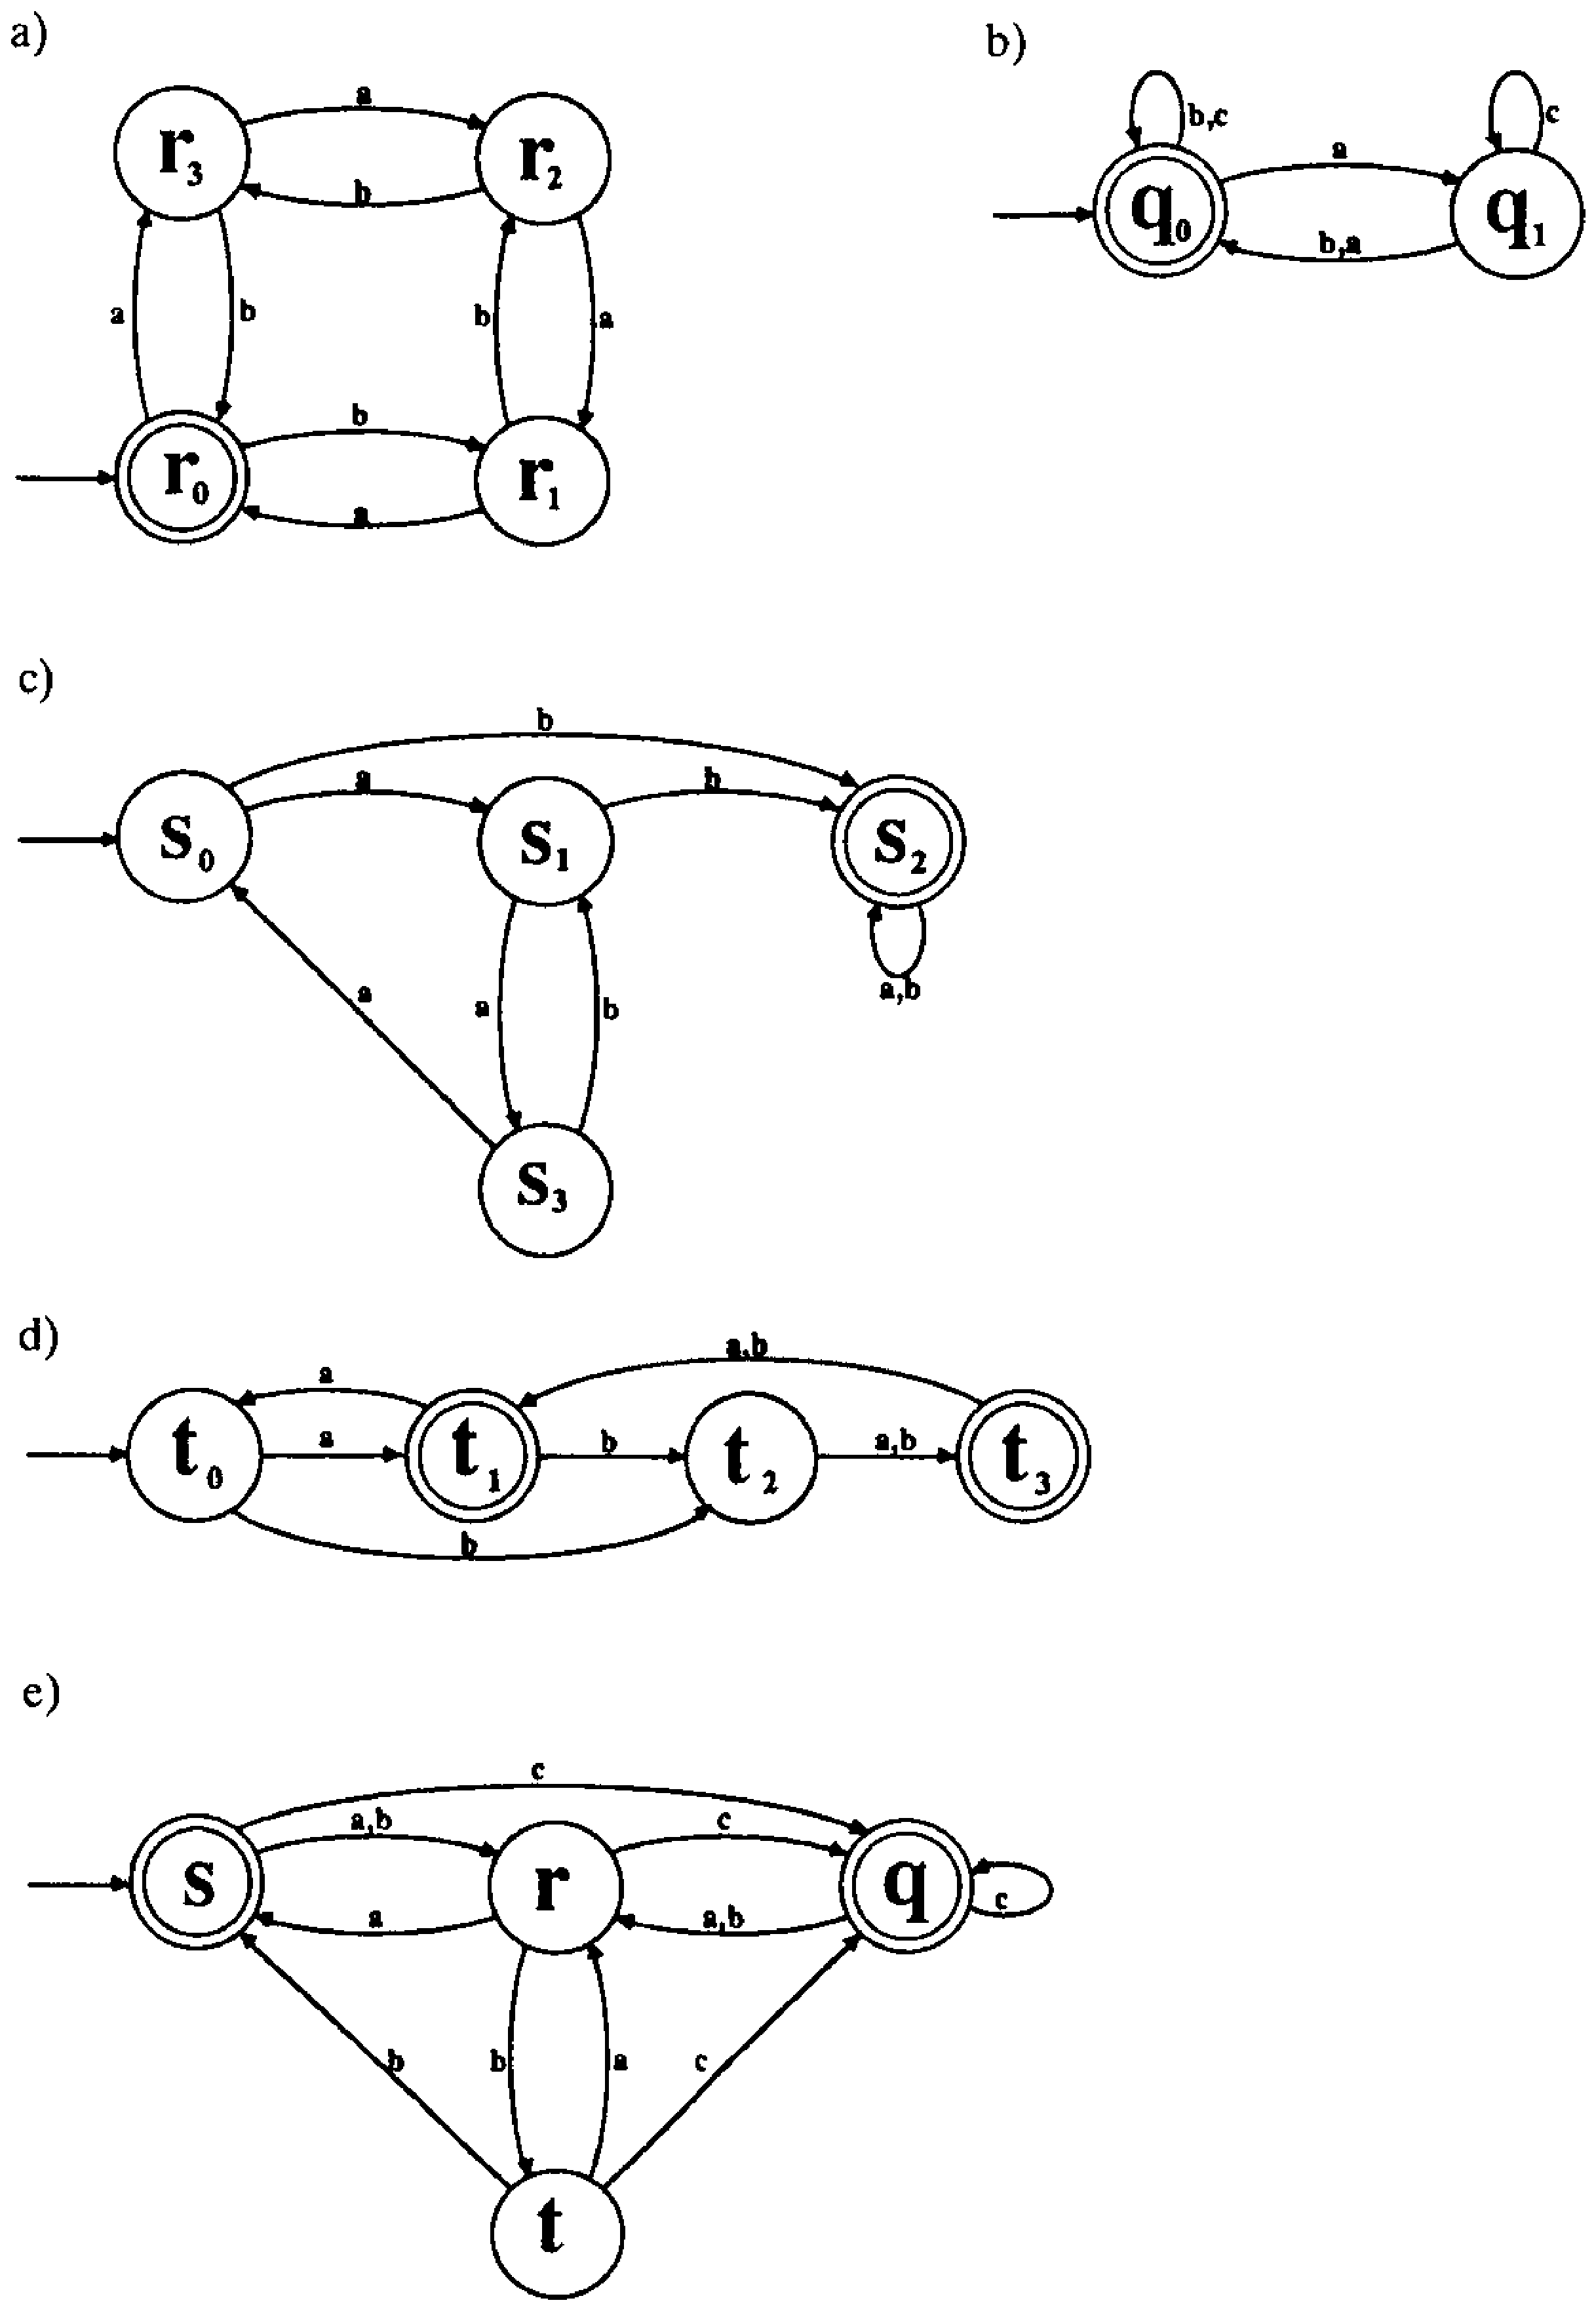
\epsfig{figure=ToFAfigures/fig8-4.eps,width=5.2in}}
\caption{Automata for Exercise 8.31}\label{fig-8.4}
\end{figure}

% Figure 8.5
\begin{figure}
\centerline{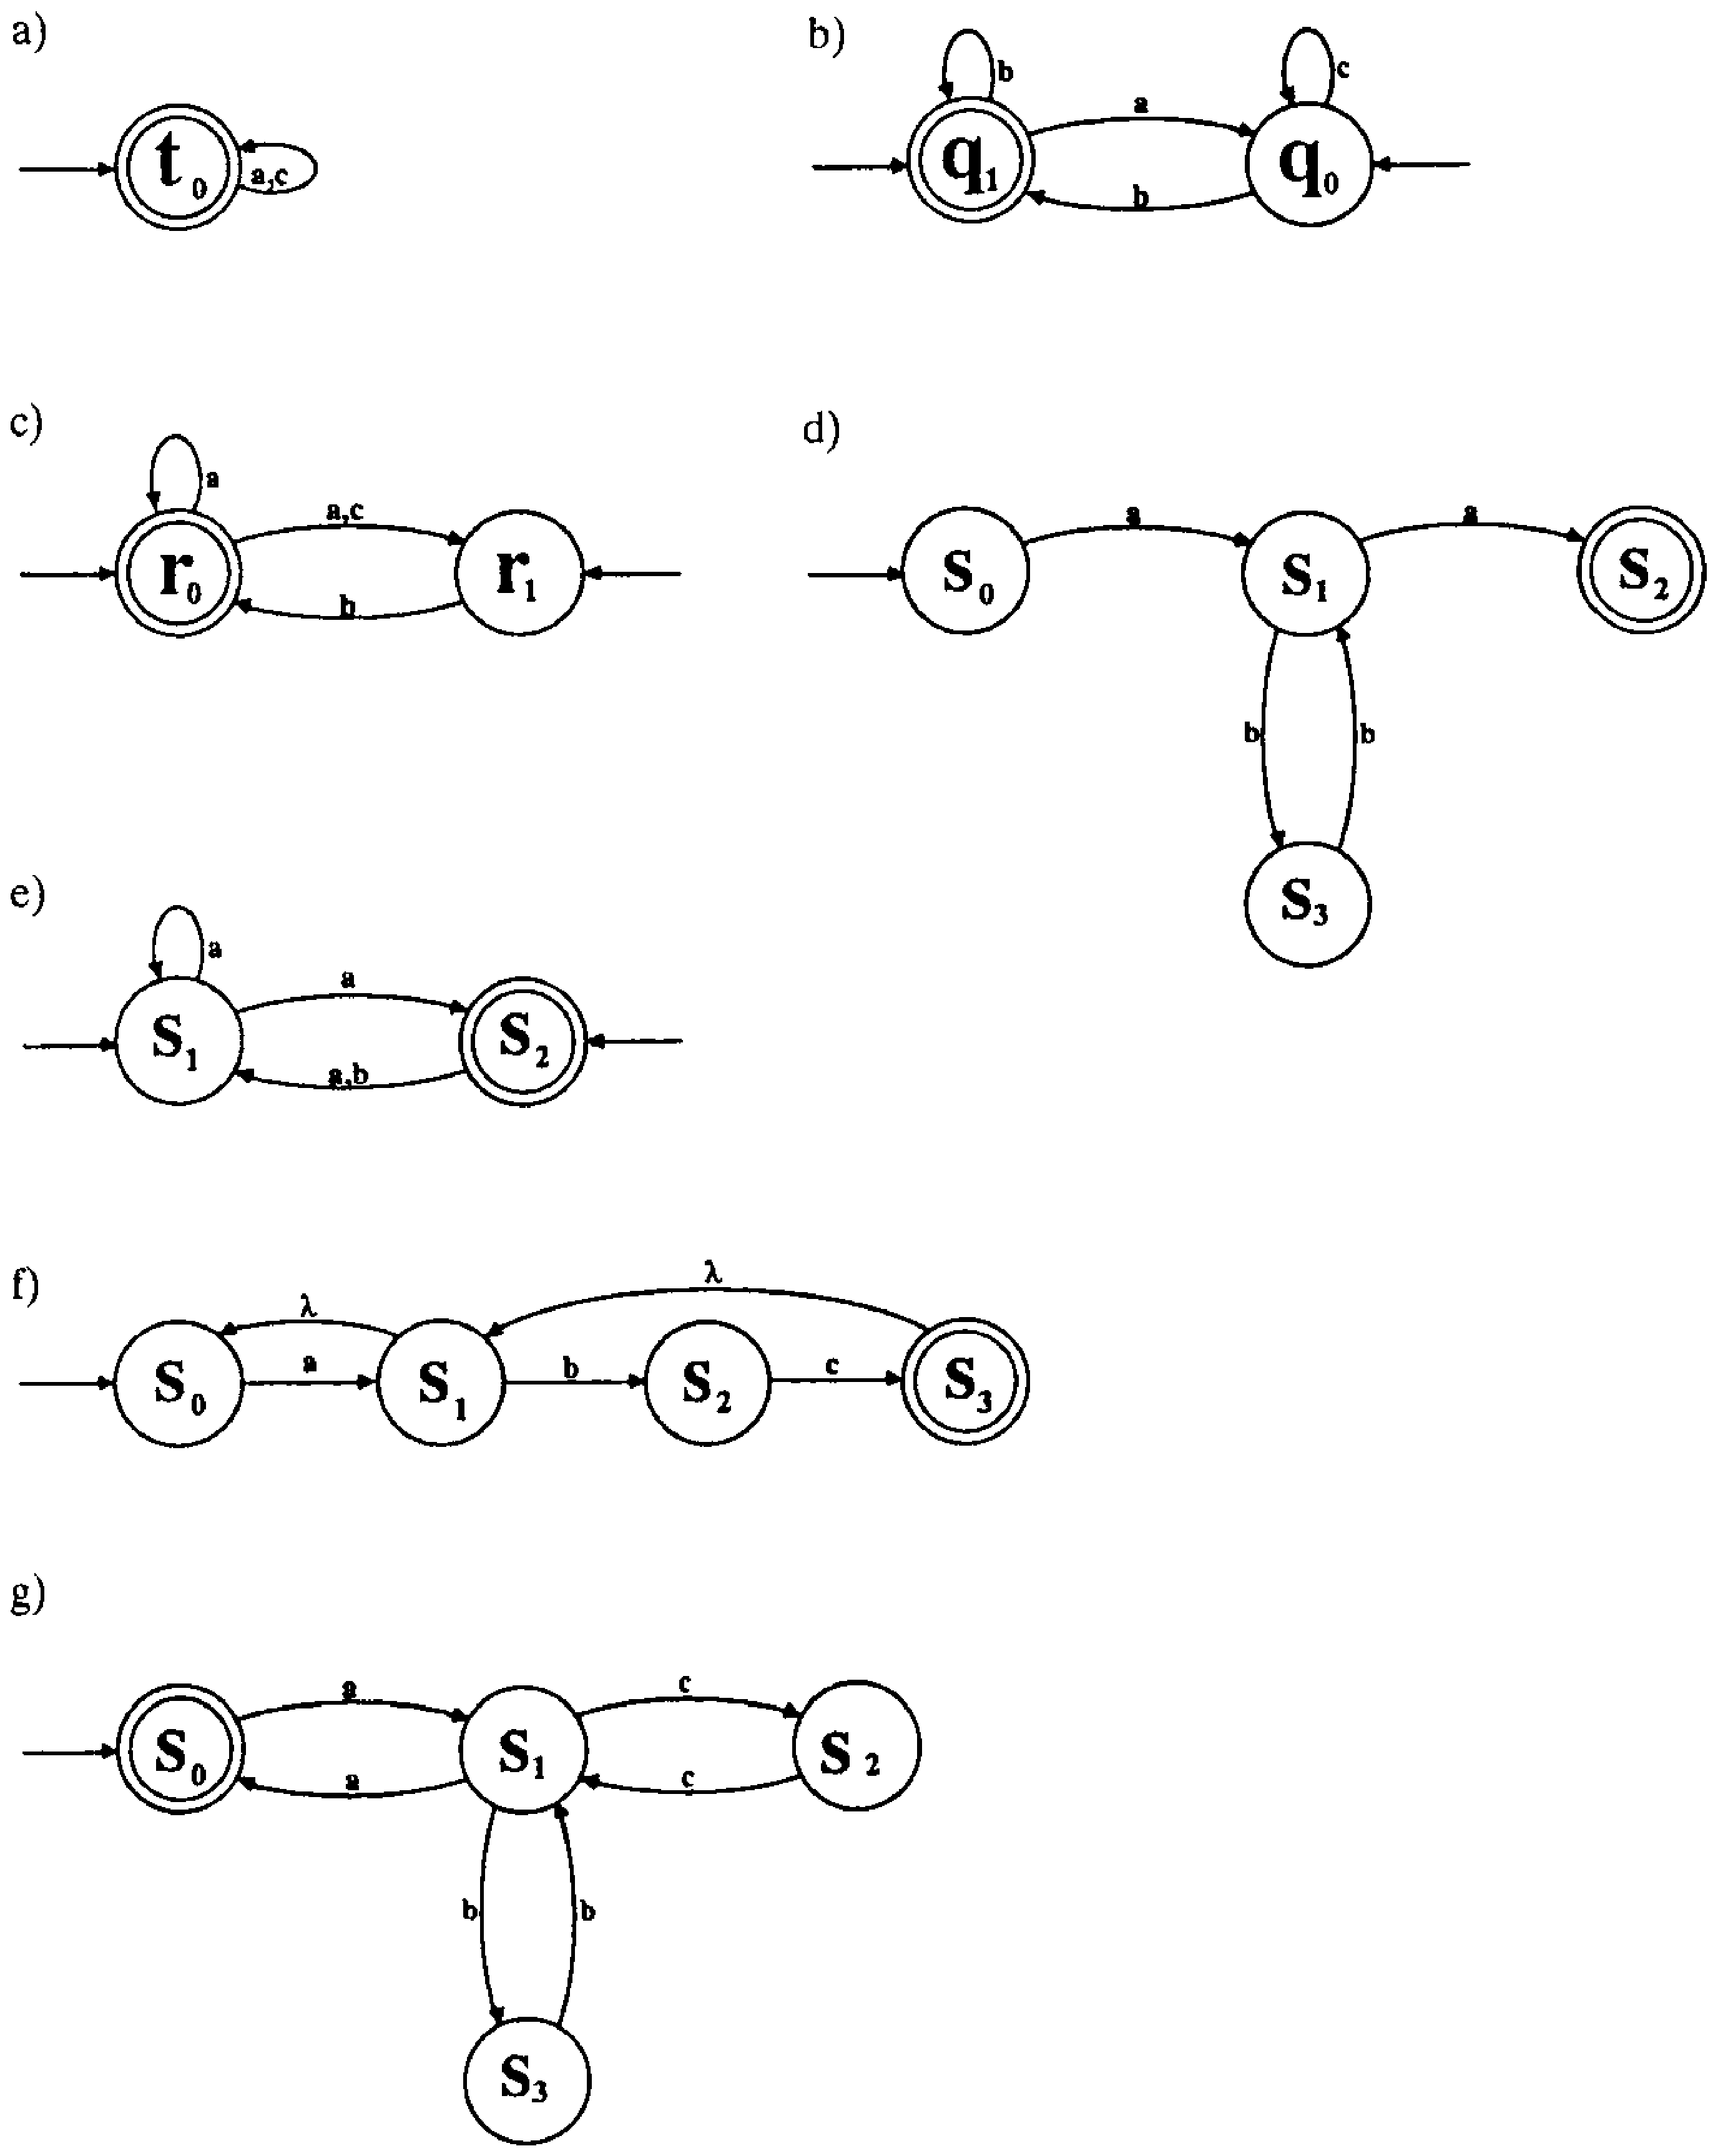
\epsfig{figure=ToFAfigures/fig8-5.eps,width=5.2in}}
\caption{Automata for Exercise 8.32}\label{fig-8.5}
\end{figure}

\item Let $\Sigma=\{\pmb{a},\pmb{b}\}$.  Define context-free grammars for the following languages:
\begin{enumerate}
\item $L_1 =$ all words over $\Sigma^*$ for which the last letter matches the
first letter.
\item $L_2 =$ all odd-length words over $\Sigma^*$ for which the first letter
matches the center letter.
\item $L_3 =$ all words over $\Sigma^*$ for which the last letter matches none
of the other letters.
\item $L_4 =$ all even-length words over $\Sigma^*$ for which the two center
letters match.
\item $L_5 =$ all odd-length words over $\Sigma^*$ for which the center letter
matches none of the other letters.
\item Which of the above languages are regular?
\end{enumerate}

\item Define context-free grammars for the following languages:
\begin{enumerate}
\item $L=\{x\in\{\pmb{a},\pmb{b}\}^*\ |\ \ |x|_a < |x|_b\}$
\item $G=\{x\in\{\pmb{a},\pmb{b}\}^*\ |\ \ |x|_a \geq |x|_b\}$
\item $K=\{w\in\{\pmb{0},\pmb{1}\}^*\ |\ w=w^r\}$
\item $\Phi=\{x\in\{\pmb{a},\pmb{b},\pmb{c}\}^*\ |\ \exists i,j,k\in\NN\ni x =
\pmb{a}^j\pmb{b}^k\pmb{c}^m$, where $j \geq 3$ and $k = m\}$
\end{enumerate}

\item Define context-free grammars for the following languages:
\begin{enumerate}
\item $L_1=\{x\in\{\pmb{a},\pmb{b}\}^*\ |\ \ |x|_a = 2|x|_b\}$
\item $L_2=\{x\in\{\pmb{a},\pmb{b}\}^*\ |\ \ |x|_a \not= |x|_b\}$
\item The set of all postfix expressions over the alphabet $\{\pmb{A},\pmb{B},
\pmb{+},\pmb{-}\}$
\item The set of all parenthesized infix expressions over the alphabet $\{\pmb{A},
\pmb{B},\pmb{+},\pmb{-},\pmb{(},\pmb{)}\}$
\end{enumerate}

\item Define context-sensitive grammars for the following languages:
\begin{enumerate}
\item $\Gamma = \{x\in\{\pmb{0},\pmb{1},\pmb{2}\}^*\ |\ \exists w\in\{\pmb{0},
\pmb{1}\}^*\ni x=w\cdot 2\cdot w\}=\{\pmb{2},\pmb{121},\pmb{020},\pmb{11211},
\pmb{10210},\ldots\}$
\item $\Phi = \{x\in\{\pmb{b}\}^*\ |\ \exists j\in\NN\ni |x|=2^j\}=\{\pmb{b},
\pmb{bb},\pmb{bbbb},\pmb{b}^8,\pmb{b}^{16},\pmb{b}^{32},\ldots\}$
\end{enumerate}

\item Consider the grammar
\[ G=\langle\{A,B,S\},\{\pmb{a},\pmb{b},\pmb{c}\},S,\{S\rightarrow\pmb{a}SB
	\pmb{c},S\rightarrow\lambda,SB\rightarrow\pmb{b}S,\pmb{c}B\rightarrow B
	\pmb{c}\}\rangle \]
Show that this context-sensitive grammar is \emph{not} equivalent to $G''$ given in
Example 8.3, where
\[ G'' = \langle\{A,B,S,T\},\{\pmb{a},\pmb{b},\pmb{c}\},S,\{S\rightarrow\pmb{a}SB
	\pmb{c},S\rightarrow T,T\rightarrow\lambda,TB\rightarrow\pmb{b}T,\pmb{c}
	B\rightarrow B\pmb{c}\}\rangle \]

\item Design context-free grammars that accept:
\begin{enumerate}
\item $L_1=\pmb{a}^*(\pmb{b}\cup\pmb{c})^*\cap\{x\in\{\pmb{a},\pmb{b},\pmb{c}\}^*
\ |\ \ |x|_a = |x|_b + |x|_c\}$
\item $L_2 = \{x\in\{\pmb{a},\pmb{b},\pmb{c}\}^*\ |\ \exists i,j,k\in\NN \ni x =
\pmb{a}^i\pmb{b}^j\pmb{c}^k$, where $i + j = k\}$
\item $L_3 = \{x\in\{\pmb{a},\pmb{b},\pmb{c}\}^*\ |\ \ |x|_a + |x|_b = |x|_c\}$
\end{enumerate}

\item Refer to Definition \ref{dfn-8.4} and prove that $L(G') = L(G) \cup \{\lambda\}$.

\item Refer to Definition \ref{dfn-8.6} and prove that $L(G') = L(G) \cup \{\lambda\}$.

\item \begin{enumerate}
\item Show that if $G$ is in the form specified in Theorem \ref{thm-8.8}, so is the $G_*$ described in
Theorem \ref{thm-8.5}.
\item Give an example that shows that, even if $G_1$ and $G_2$ are in the form
specified in Theorem \ref{thm-8.8}, the grammar $G^{\cup}$ described in Theorem \ref{thm-8.4} may
not be.
\item Is your construction for $G^\bullet$ in Example 8.18 normal form preserving?
\end{enumerate}

\item Given two left-linear grammars $G_1$ and $G_2$, give a set of rules to
find a new left-linear grammar that will generate:
\begin{enumerate}
\item $L(G_1) \cup L(G_2)$
\item $L(G_1)\cdot L(G_2)$
\item $L(G_1)^*$
\end{enumerate}
\end{enumerate}

% Chapter, Section, Theorem, Corollary, Lemma, Definition, Table, Figure, {\bf 
\chapter{Context-Free Grammars}\label{ch-9}

The preceding chapter explored the properties of the type 3 grammars. The next
class of grammars in the language hierarchy, the \emph{type 2} or
\emph{context-free} grammars, are central to the linguistic aspects of computer
science. Context-free grammars were originally used to help specify natural
languages and are thus well-suited for defining computer languages. These
context-free grammars represent a much wider class of languages than did the
regular grammars. Due to the need for balancing parentheses and matched
begin-end pairs (among other things), the language Pascal cannot be specified by
a regular grammar, but it can be defined with a context-free grammar.
Programming languages are specifically designed to be representable by
context-free grammars in order to take advantage of the desirable properties
inherent in type 2 grammars. These properties are explored in this chapter,
while Chapter \ref{ch-10} investigates the generalized automata corresponding to
context-free languages.

\section{Parse Trees}\label{sec-9.1}

Derivations in a context-free grammar are similar to those of regular grammars,
and the definition of derivation given below is compatible with that given in
Definition \ref{dfn-8.8}.

% Definition 9.1
\begin{dfn}\label{dfn-9.1}
Let $\Sigma$ be any alphabet, $G=\langle\Omega,\Sigma,S,P\rangle$ be a
right-linear grammar, $\alpha A\gamma\in(\Sigma\cup\Omega)^*$, and $A\rightarrow
\beta$ be a production in $P$. We will say that $\alpha\beta\gamma$ can be
\emph{directly derived} from $\alpha A\gamma$ by applying the production $A
\rightarrow\beta$, and write $\alpha A\gamma\Rightarrow\alpha\beta\gamma$.
Furthermore, if $(\alpha_1\Rightarrow\alpha_2)\wedge(\alpha=2\Rightarrow\alpha_3)
\wedge\cdots\wedge(\alpha_{n-1}\Rightarrow\alpha_n)$, then we will say that
$\alpha_1$ derives $\alpha_n$ and write $\alpha_1\DRightarrow\alpha_n$.
\end{dfn}

As with Definition \ref{dfn-8.8}, $\alpha_1\DRightarrow\alpha_1$ in zero steps. In
generating a particular string, regular grammars typically allowed only a single
sequence of applicable productions. Context-free grammars are generally more
robust, as shown by Example 9.4, which illustrates several derivations for a
single string.

The special nature of the productions in a context-free grammar, which
replace a single nonterminal with a string of symbols, allow derivations to be
diagrammed in a treelike structure, much as sentences are diagrammed in English.
For example, the rules of English specify that a sentence is composed of a
subject followed by a predicate, which is reflected in the production
\[ \text{\<sentence\>}\rightarrow \text{\<subject\>}\text{\<predicate\>} \]
Other rules include
\[ \text{\<noun phrase\>}\rightarrow\text{\<modifier\>}\text{\<noun\>} \]
and
\[ \text{\<predicate\>}\rightarrow\text{\<verb\>}\text{\<prepositional
	phrase\>} \]
A specific sequential application of these and other rules to form an English
sentence might be diagrammed as shown in Figure \ref{fig-9.1}. Such diagrams are called
\emph{parse trees} or \emph{derivation trees}.

% Definition 9.2
\begin{dfn}\label{dfn-9.2}
A \emph{\Index{parse tree}} or \emph{\Index{derivation tree}} for a regular or
context-free grammar $G=\langle\Omega,\Sigma,S,P\rangle$ is a labeled, ordered
tree in which the root node is labeled $S$, and the $n$ subtrees of a node
labeled $A$ are labeled $\alpha_1$ through $\alpha_n$ only if $A\rightarrow
\alpha_1\cdot\alpha_2\cdots\alpha_n$ is a production in $P$, and each $\alpha_i \in
(\Omega\cup\Sigma)$. However, if $B\rightarrow\lambda$ is a production in $P$,
then a node labeled $B$ may instead have a single subtree labeled $\lambda$. The
parse tree is called \emph{complete} if no leaf is labeled with a nonterminal.
\end{dfn}

Recall that for context-free grammars only the start symbol $Z$ can have a
production of the form $B\rightarrow\lambda$; regular grammars are allowed to
have several such rules.

\subsection*{Example 9.1}

As illustrated in Figure \ref{fig-9.1}, a parse tree shows a particular sequence of
substitutions allowed by a given grammar. A left-to-right rendering of the
leaves of this complete parse tree yields the terminal string ``the check is in
the mail.''

% Figure 9.1
\begin{figure}
\centerline{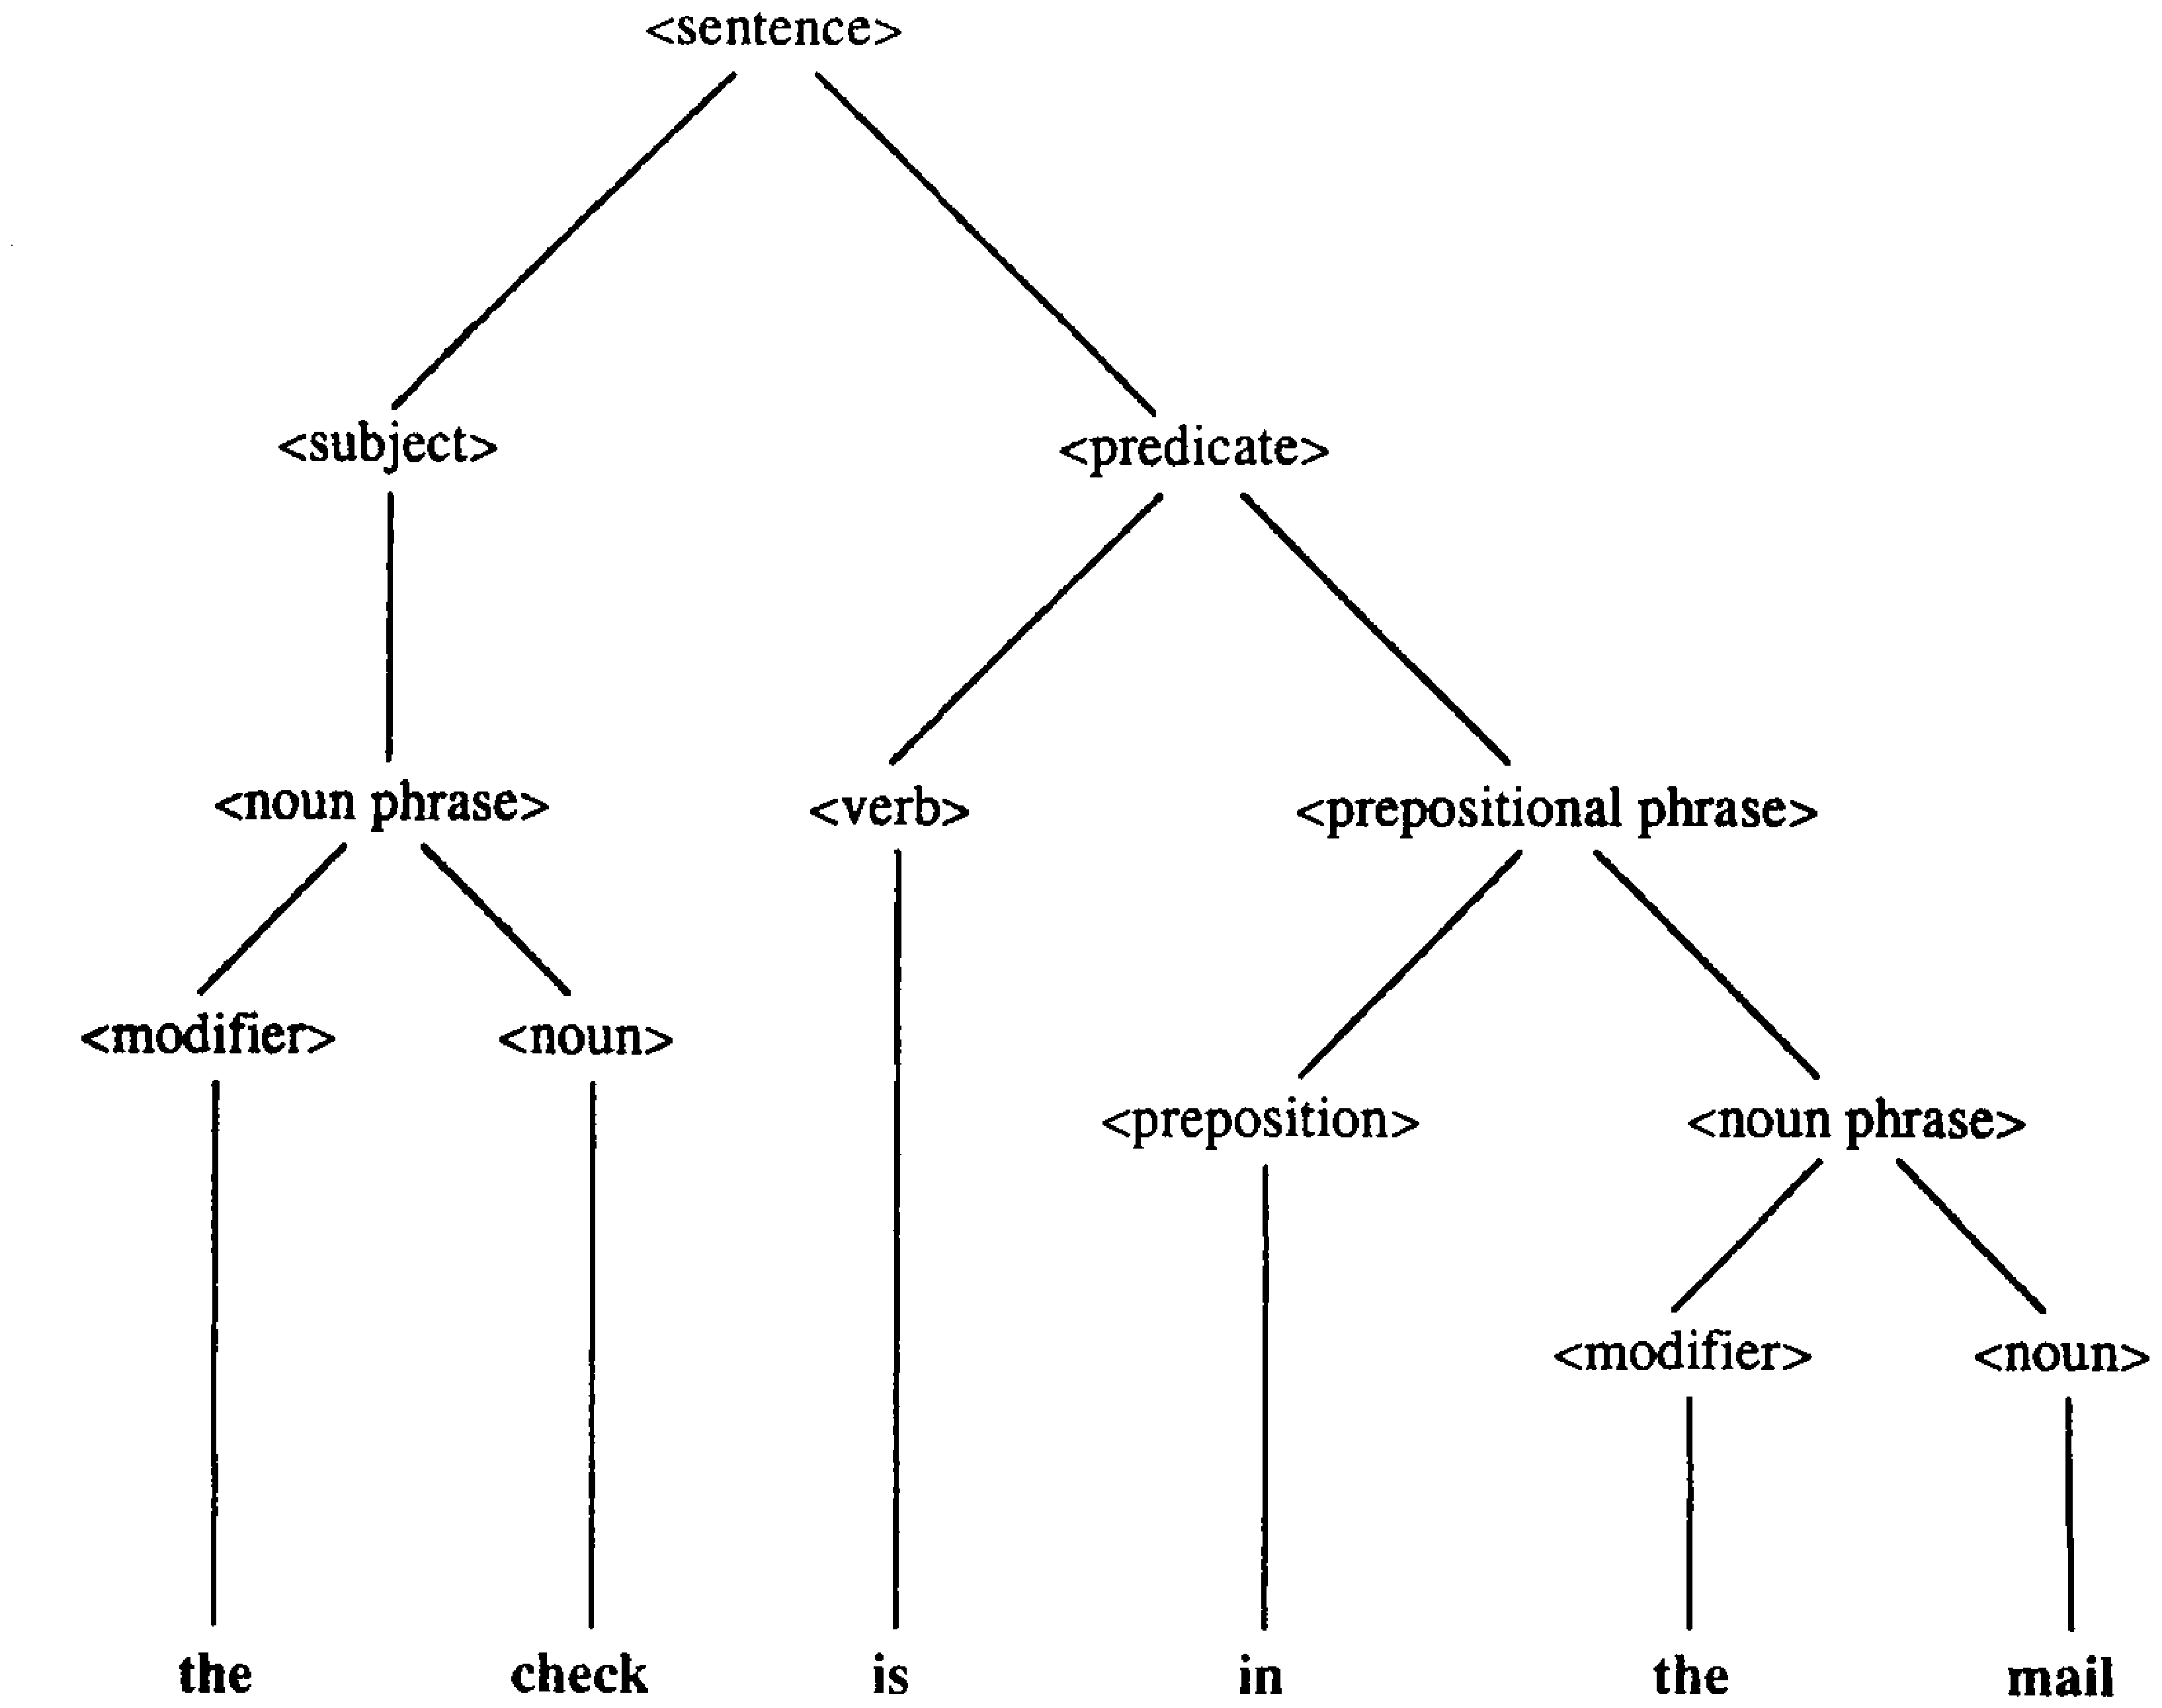
\epsfig{figure=ToFAfigures/fig9-1.eps,width=5.5in}}
\caption{A parse tree for the English grammar}\label{fig-9.1}
\end{figure}

\subsection*{Example 9.2}

Regular grammars form parse trees that are much more restrictive; at any given
level in the tree, only one node can be labeled with a nonterminal. Figure \ref{fig-9.2}
shows the parse tree for the word $\pmb{aaabaa}$ from the grammar
\[ G_1 = \langle\{T,S\},\{\pmb{a},\pmb{b}\},S,\{S\rightarrow\pmb{a}S,S
	\rightarrow\pmb{b}T,T\rightarrow\pmb{aa}\}\rangle. \]
In general, since productions in a right-linear grammar allow only the rightmost
symbol to be a nonterminal, parse trees for right-linear grammars will only
allow the rightmost child of a node to have a nontrivial subtree.

\subsection*{Example 9.3}\index{regular expression grammar}

Given a context-free grammar $G$, a common task required of compilers is to scan
a proposed terminal string $x$ belonging to $L(G)$ and build a parse tree
corresponding to $x$. If $G$ is the ``regular expression'' grammar defined in
Example 8.2, $G=\langle\{R\},\{\pmb{a},\pmb{b},\pmb{c},\pmb{(},\pmb{)},
\pmb{\epsilon},\pmb{\emptyset},\pmb{\cup},\pmb{\cdot},\pmb{^*}\},R,\{R
\rightarrow\pmb{a}|\pmb{b}|\pmb{c}|\pmb{\epsilon}|\pmb{\emptyset}|\pmb{(}R\pmb{\cdot} R\pmb{)}|\pmb{(}R
\pmb{\cup} R\pmb{)}|R\pmb{^*}\}\rangle$ and $x$ is $\pmb{((a\cup b)^*\!\!\cdot c)}$, the
desired result would be a representation of the tree shown in Figure \ref{fig-9.3}.

% Figure 9.2
\begin{figure}
\centerline{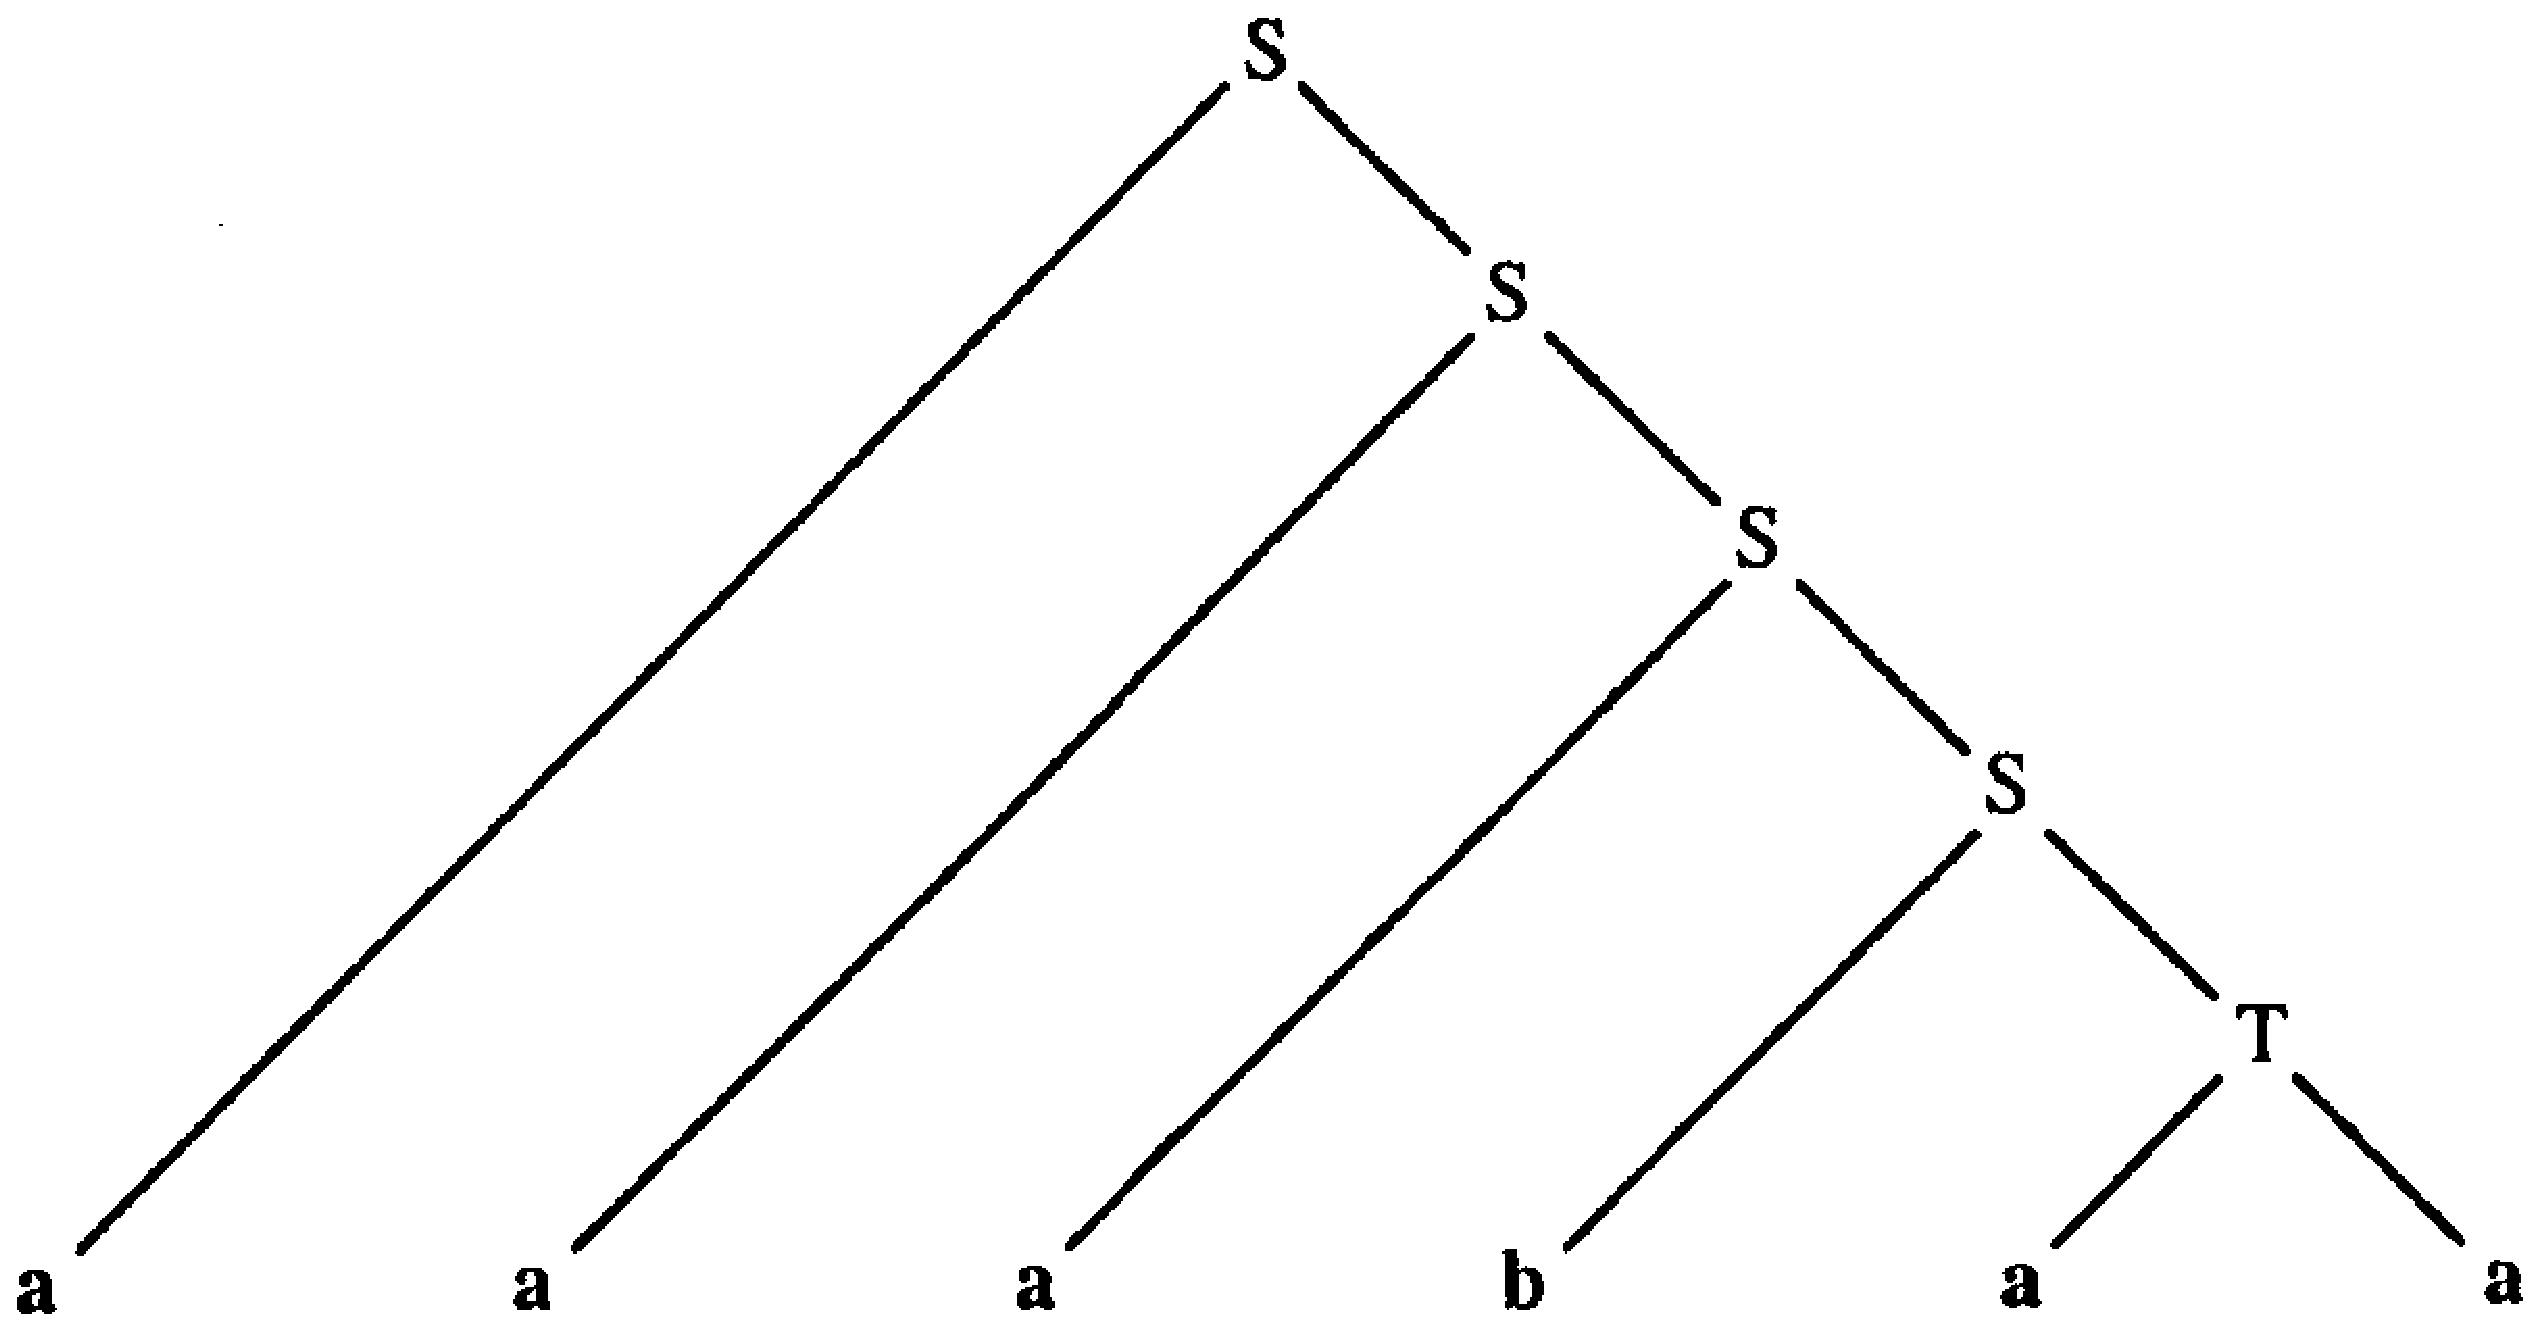
\epsfig{figure=ToFAfigures/fig9-2.eps,width=4.5in}}
\caption{The parse tree discussed in Example 9.2}\label{fig-9.2}
\end{figure}

In a perfect world of perfect programmers, it might be appropriate to assume
that $x$ can definitely be generated by the productions in $G$. In our world,
however, compilers must unfortunately perform the added task of determining
whether it is possible to generate the proposed terminal string $x$, that is,
whether the file presented represents a syntactically correct program. This is
typically done as the parse trees are being built, and discrepancies are
reported to the user. For the ``regular expression'' grammar used in Example
9.3, there is an algorithm for scanning the symbols of proposed strings such as
$\pmb{((a\cup b)^*\!\!\cdot c)}$ to determine whether a parse tree can be
constructed. In the case of a string like $\pmb{((a\cup b)}$, no such parse
tree exists, and the string therefore cannot be generated by the grammar. If the
productions of a grammar follow certain guidelines, the task of finding the
correct scanning algorithm is greatly simplified. The desired properties that
should be inherent in a programming language grammar are investigated later in
the text.

In a separate phase, after the parse trees are found, the compiler then uses
the trees and other constructs to infer meaning to the program, that is, to
generate appropriate machine code that reflects the advertised meaning (that is,
the \Index{semantics}) of the program statements. For example, the parse tree for
$((\pmb{a}\cup\pmb{b})^*\cdot\pmb{c})$ in Figure \ref{fig-9.3} clearly shows both the
order in which the operators $\cup$, $\cdot$, and $^*$ should be applied and the
expressions to which they should be applied.

Given a particular complete parse tree for a string $x$, there may be some
freedom in the order in which the associated productions are applied.

% Figure 9.3
\begin{figure}
\centerline{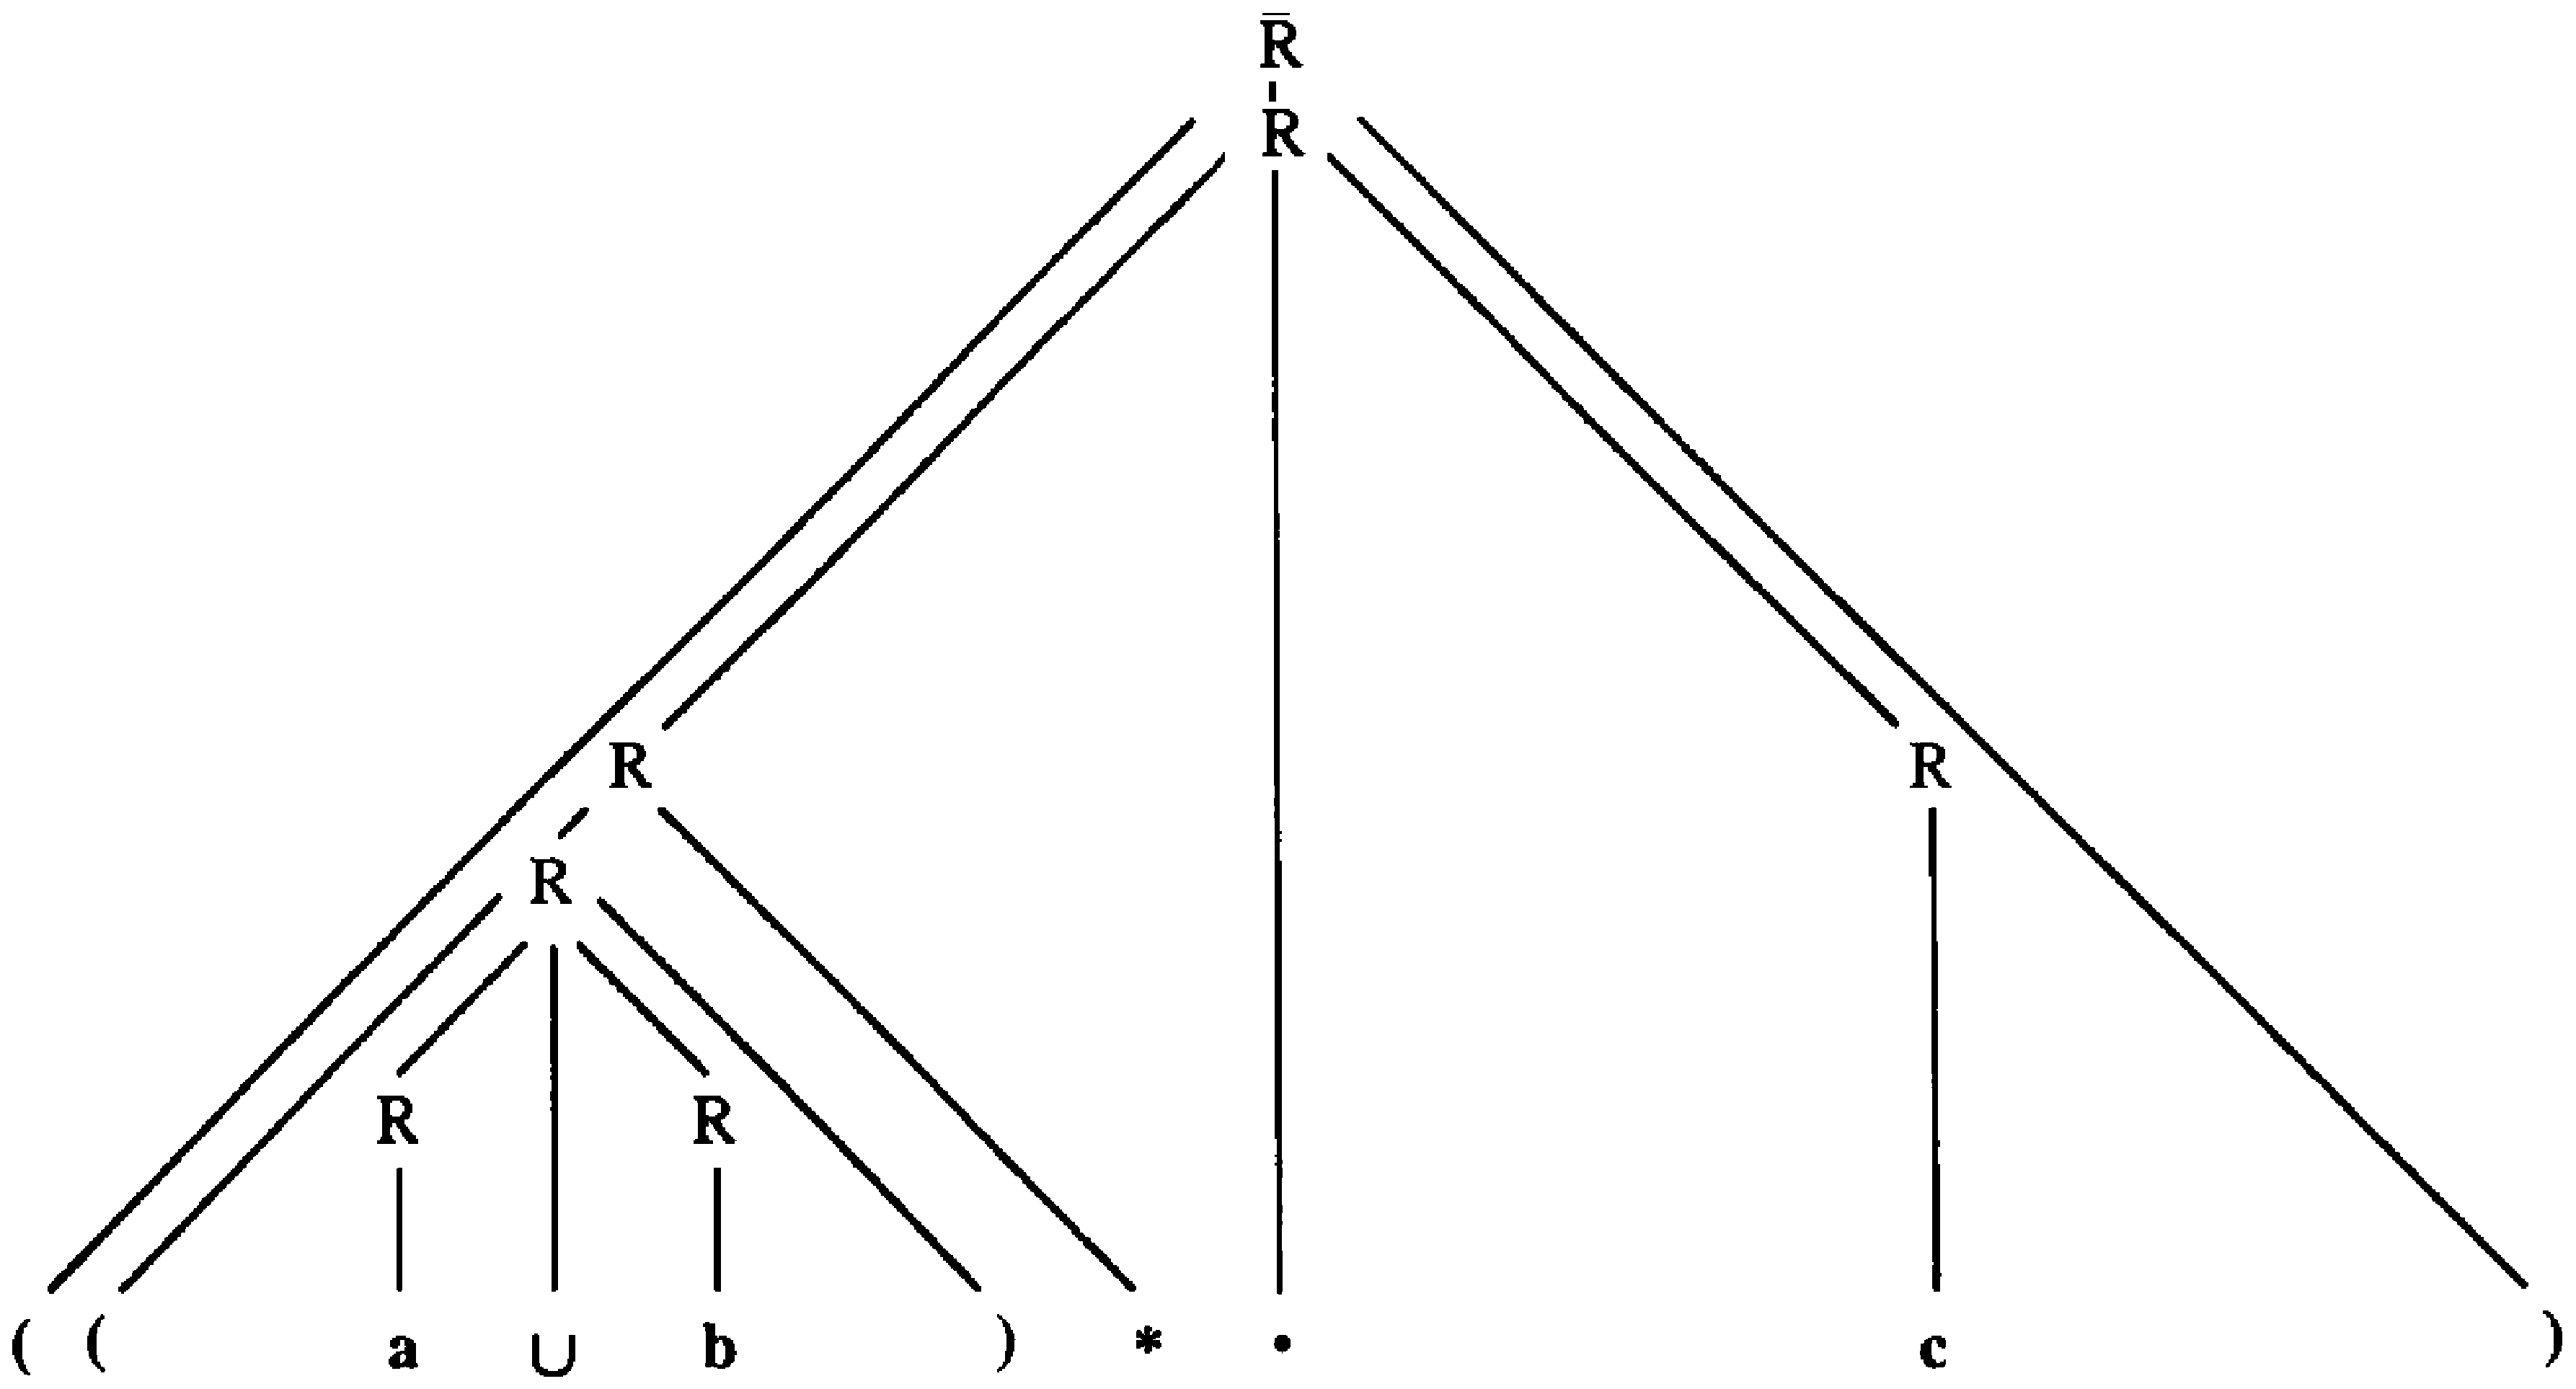
\epsfig{figure=ToFAfigures/fig9-3.eps,width=6.0in}}
\caption{The parse tree discussed in Example 9.3}\label{fig-9.3}
\end{figure}

\subsection*{Example 9.4}

For the grammar
\[ G=\langle\{R\},\{\pmb{a},\pmb{b},\pmb{c},\pmb{(},\pmb{)},
\pmb{\epsilon},\pmb{\emptyset},\pmb{\cup},\pmb{\cdot},\pmb{^*}\},R,\{R
\rightarrow\pmb{a}|\pmb{b}|\pmb{c}|\pmb{\epsilon}|\pmb{\emptyset}|
\pmb{(}R\pmb{\cdot} R\pmb{)}|\pmb{(}R\pmb{\cup} R\pmb{)}|R\pmb{^*}\}\rangle \]
%\[ G=\langle\{R\},\{\pmb{a},\pmb{b},\pmb{c},\pmb{(},\pmb{)},\pmb{\epsilon},
%	\pmb{\emptyset},\pmb{\cup},\pmb{\cdot},\pmb{^*}\},R,\{R\rightarrow
%	\pmb{a}|\pmb{b}|\pmb{c}|\pmb{\epsilon}|\pmb{\emptyset}|(R\cdot R)|(R\cup
%	R)|R^*\} \]
each of the following are valid derivations of the string $x=\pmb{((a\cup b)^*\!\!\cdot c)}$.

\noindent\emph{Derivation 1:}
\begin{center}\begin{tabular}{r@{ $\Rightarrow$ }l}
$R$ & $(R\cdot R)$ \\
& $(R^*\cdot R)$ \\
& $((R\cup R)^*\cdot R)$ \\
& $((\pmb{a}\cup R)^*\cdot R)$ \\
& $((\pmb{a}\cup\pmb{b})^*\cdot R)$ \\
& $((\pmb{a}\cup\pmb{b})^*\cdot\pmb{c})$
\end{tabular}\end{center}
\emph{Derivation 2:}
\begin{center}\begin{tabular}{r@{ $\Rightarrow$ }l}
$R$ & $(R\cdot R)$ \\
& $(R^*\cdot R)$ \\
& $((R\cup R)^*\cdot R)$ \\
& $((R\cup R)^*\cdot\pmb{c})$ \\
& $((R\cup\pmb{b})^*\cdot\pmb{c})$ \\
& $((\pmb{a}\cup\pmb{b})^*\cdot\pmb{c})$
\end{tabular}\end{center}
\emph{Derivation 3:}
\begin{center}\begin{tabular}{r@{ $\Rightarrow$ }l}
$R$ & $(R\cdot R)$ \\
& $(R\cdot\pmb{c})$ \\
& $(R^*\cdot\pmb{c})$ \\
& $((R\cup R)^*\cdot\pmb{c})$ \\
& $((\pmb{a}\cup R)^*\cdot\pmb{c})$ \\
& $((\pmb{a}\cup\pmb{b})^*\cdot\pmb{c})$
\end{tabular}\end{center}
\emph{Derivation 4:}
\begin{center}\begin{tabular}{r@{ $\Rightarrow$ }l}
$R$ & $(R\cdot R)$ \\
& $(R\cdot\pmb{c})$ \\
& $(R^*\cdot\pmb{c})$ \\
& $((R\cup R)^*\cdot\pmb{c})$ \\
& $((R\cup\pmb{b})^*\cdot\pmb{c})$ \\
& $((\pmb{a}\cup\pmb{b})^*\cdot\pmb{c})$
\end{tabular}\end{center}

% Definition 9.3
\begin{dfn}\label{dfn-9.3}\index{leftmost derivation}\index{rightmost derivation}
A derivation sequence is called a \emph{leftmost} derivation if at each
step in the sequence the leftmost nonterminal is next expanded to produce the
following step. A derivation sequence is called a \emph{rightmost}
derivation if at each step in the sequence the rightmost nonterminal is next
expanded to produce the following step.
\end{dfn}

The first of the derivations given in Example 9.4 is a \emph{leftmost}
derivation since at each step it is always the leftmost nonterminal that is
expanded to arrive at the next step. Similarly, the last of these, derivation
4, is a \emph{rightmost} derivation. There are many other possible derivations,
such as derivations 2 and 3, which are neither leftmost nor rightmost.

The restrictions on regular grammars ensure that there is never more than one
nonterminal present at any point during a derivation. This \emph{linear} nature
of regular grammars ensures that all derivations of a parse tree follow exactly
the same sequence, since there is never a choice of nonterrninals to expand.
Thus, the rightmost derivation of a parse tree in a regular grammar is always
the same as its leftmost derivation.

Parse trees in context-free grammars are generally more robust, allowing
several different derivation sequences to correspond to the same tree. For a
given parse tree, though, there is only one leftmost derivation. In Figure \ref{fig-9.4},
the nodes in the parse tree for $((\pmb{a}\cup\pmb{b})^*\!\cdot\pmb{c})$ are
numbered to show the order in which they would be visited by a \Index{preorder traversal}.
Note that the sequence in which the \emph{non}terminals would be
expanded in a leftmost derivation corresponds to the order in which they appear
in the preorder traversal.

% Figure 9.4
\begin{figure}
\centerline{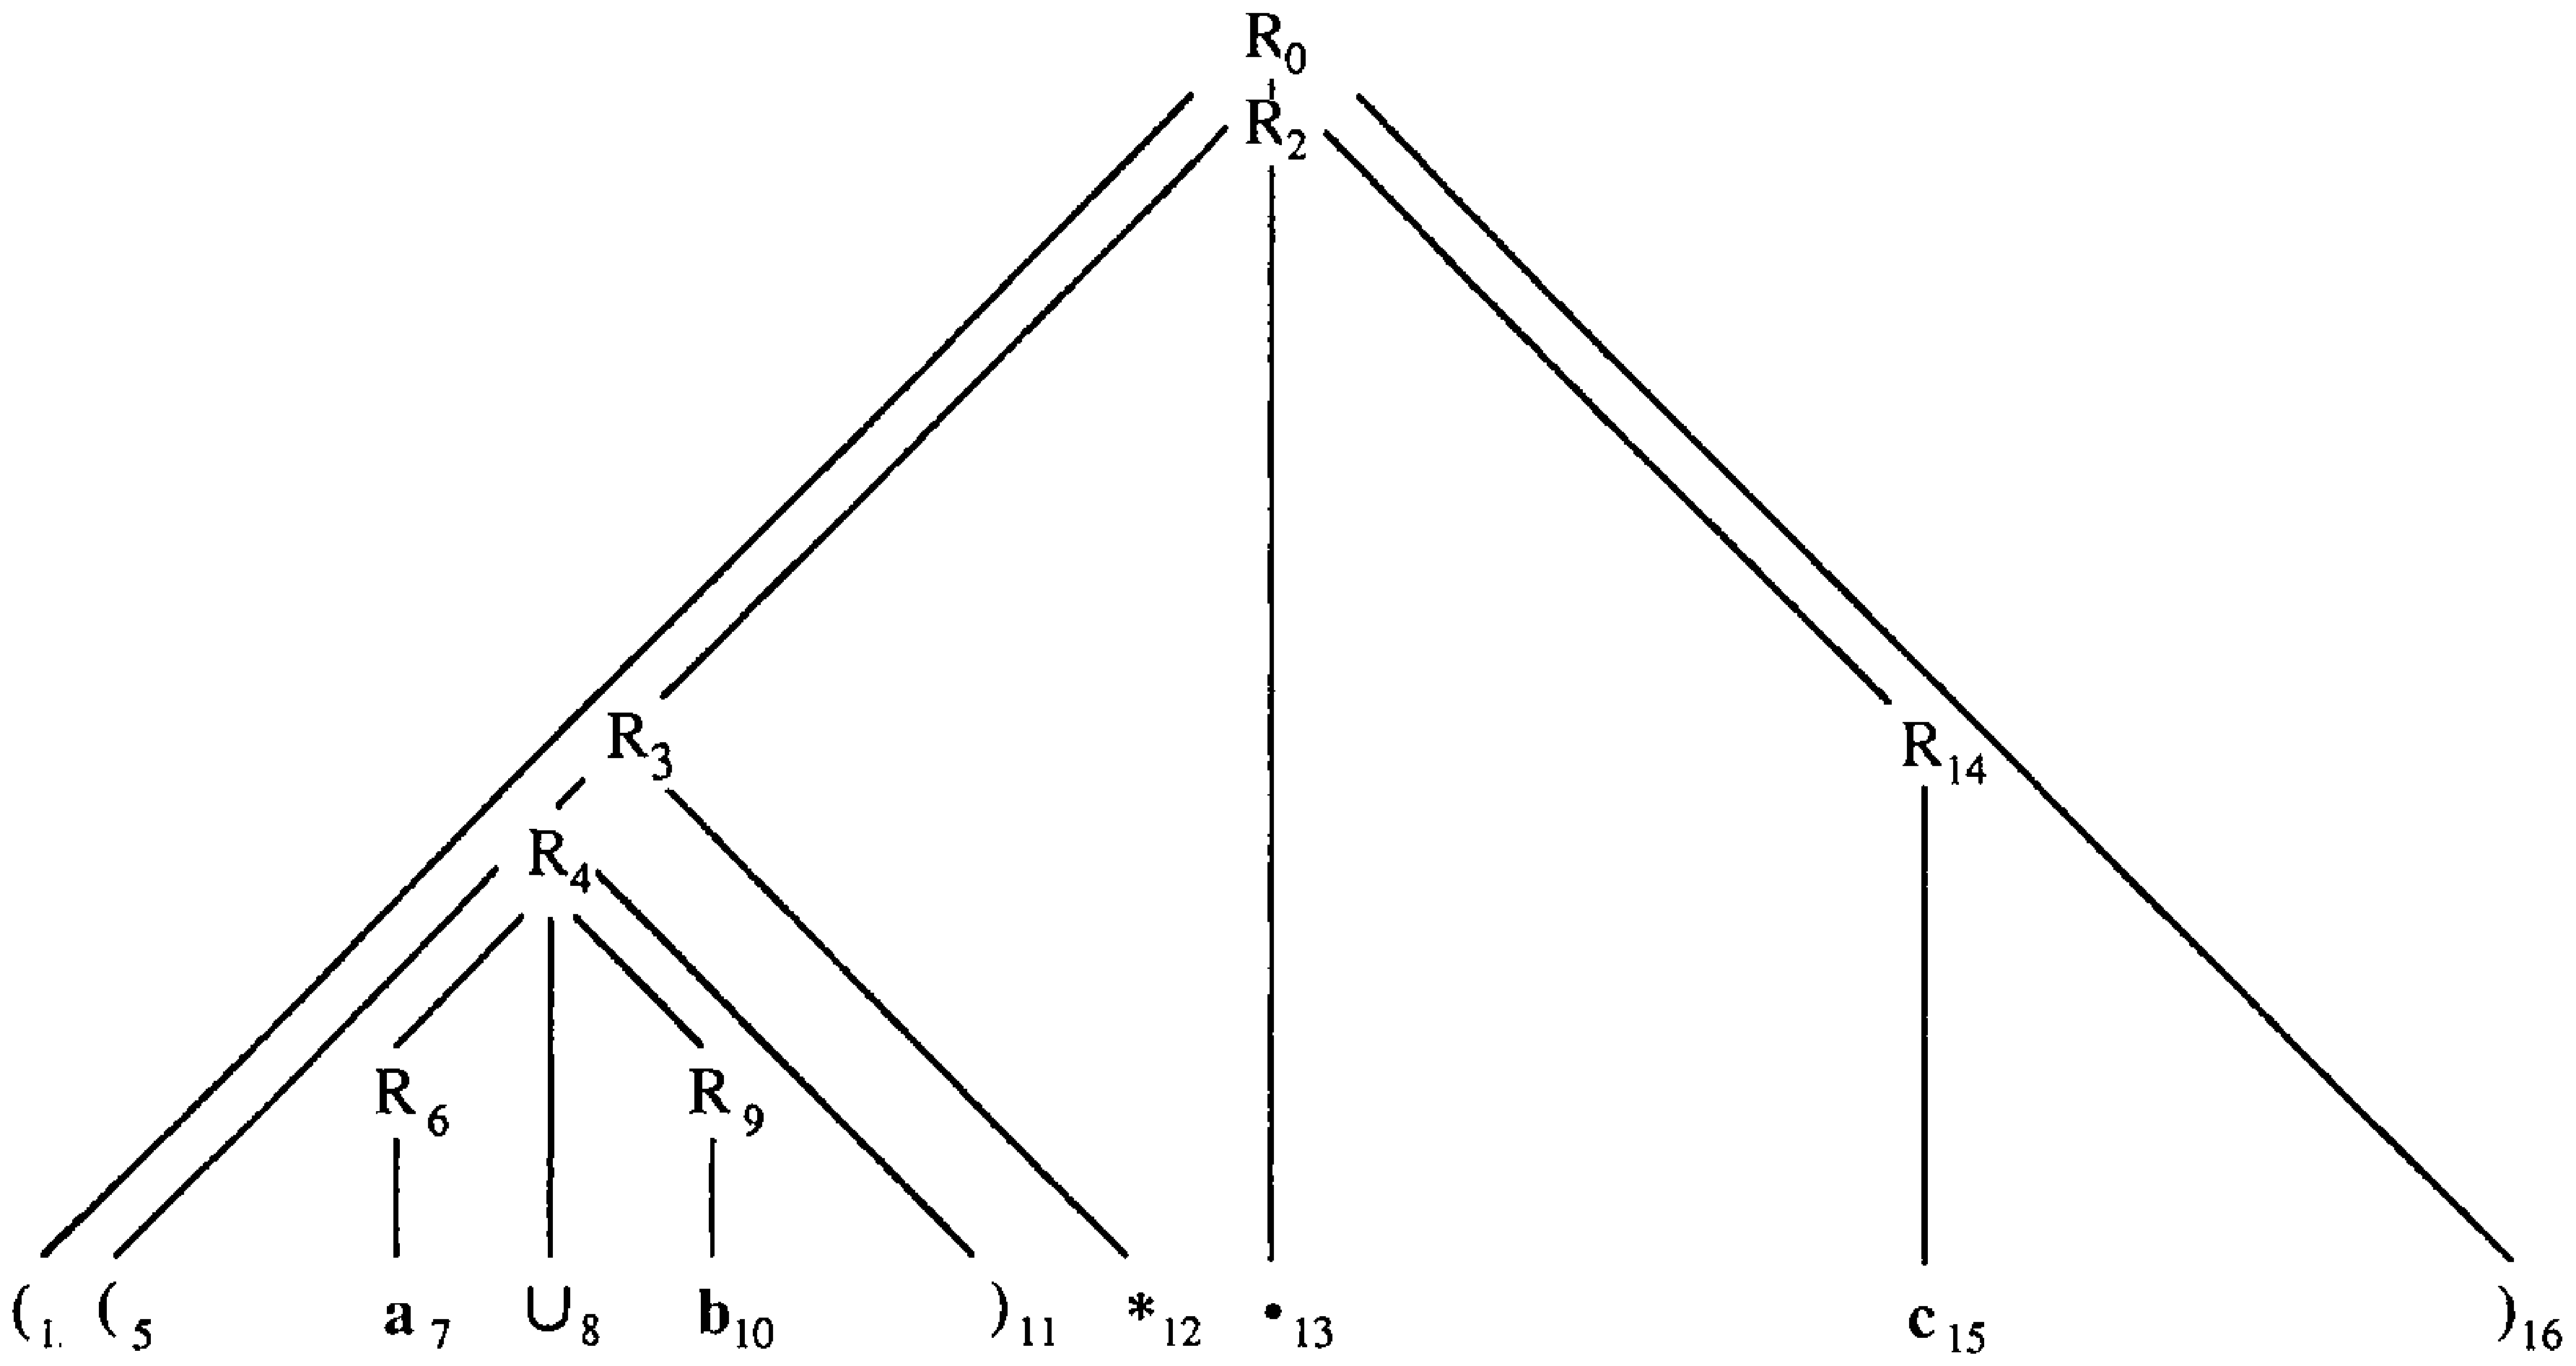
\epsfig{figure=ToFAfigures/fig9-4.eps,width=6.0in}}
\caption{The preorder traversal of the parse tree}\label{fig-9.4}
\end{figure}

\section{Ambiguity}\label{sec-9.2}

Whereas each tree corresponds to a unique leftmost derivation, it is possible
for a terminal string to have more than one leftmost derivation. This will
happen whenever a string $x$ corresponds to more than one parse tree, that is,
whenever there are truly distinct ways of applying the productions of the
grammar to form $x$. Grammars for which this can happen are called
\emph{ambiguous}.

% Definition 9.4
\begin{dfn}\label{dfn-9.4}\index{ambiguous context free grammar}\index{unambiguous grammar}
A grammar $G=\langle\Omega,\Sigma,S,P\rangle$ is called \emph{ambiguous}
if there exists a string $x\in\Sigma^*$ that corresponds to two distinct parse
trees. A grammar that is not ambiguous is called \emph{unambiguous}.
\end{dfn}

\subsection*{Example 9.5}

Consider the grammar $G_2=\langle\{S,A\},\{\pmb{a}\},S,\{S\rightarrow AA,A
\rightarrow\pmb{a}S\pmb{a},A\rightarrow\pmb{a}\}\rangle$. Figure \ref{fig-9.5} shows the
two distinct parse trees associated with the word $\pmb{aaaaa}$. Note that the
leftmost derivations corresponding to these trees are indeed different:
\begin{center}\begin{tabular}{r@{ $\Rightarrow$ }l}
$S$ & $AA$ \\
& $\pmb{a}S\pmb{a}A$ \\
& $\pmb{a}AA\pmb{a}A$ \\
& $\pmb{aa}A\pmb{a}A$ \\
& $\pmb{aaaa}A$ \\
& $\pmb{aaaaa}$
\end{tabular}\end{center}
is the sequence indicated by the parse tree in Figure \ref{fig-9.5}a, while
\begin{center}\begin{tabular}{r@{ $\Rightarrow$ }l}
$S$ & $AA$ \\
& $\pmb{a}A$ \\
& $\pmb{aa}S\pmb{a}$ \\
& $\pmb{aa}AA\pmb{a}$ \\
& $\pmb{aaa}A\pmb{a}$ \\
& $\pmb{aaaaa}$
\end{tabular}\end{center}
corresponds to Figure \ref{fig-9.5}b.

Recall that context-free grammars are used to inspect statements within a
computer program and determine corresponding parse trees. Such ambiguity is
undesirable in a grammar that describes a programming language, since it would
be unclear which of the trees should be used to infer the meaning of the string.
Indeed, this ambiguity would be intolerable if a statement could give rise to
two trees that implied different meanings, as illustrated in Example 9.6 below.
It is therefore of practical importance to avoid descriptions of languages that
entail this sort of ambiguity.

The language defined by the grammar $G_2$ in Example 9.5 is actually quite
simple. Even though $G_2$ is not a regular grammar, it can easily be shown that
$L(G_2)$ is the regular set $\{\pmb{a}^2,\pmb{a}^5,\pmb{a}^8,\pmb{a}^{11},
\pmb{a}^{14},\ldots\}$. The ambiguity is therefore not inherent in the language,
but is rather a consequence of the needlessly complex grammar used to describe
the language. A much simpler context-free grammar is given by $G_3=\langle\{T\},
\{\pmb{a}\},T,\{T\rightarrow\pmb{aaa}T,T\rightarrow\pmb{aa}\}\rangle$. This
grammar happens to be right linear and is definitely not ambiguous.

\subsection*{Example 9.6}\index{subtraction grammar}

% Figure 9.5
\begin{figure}
\centerline{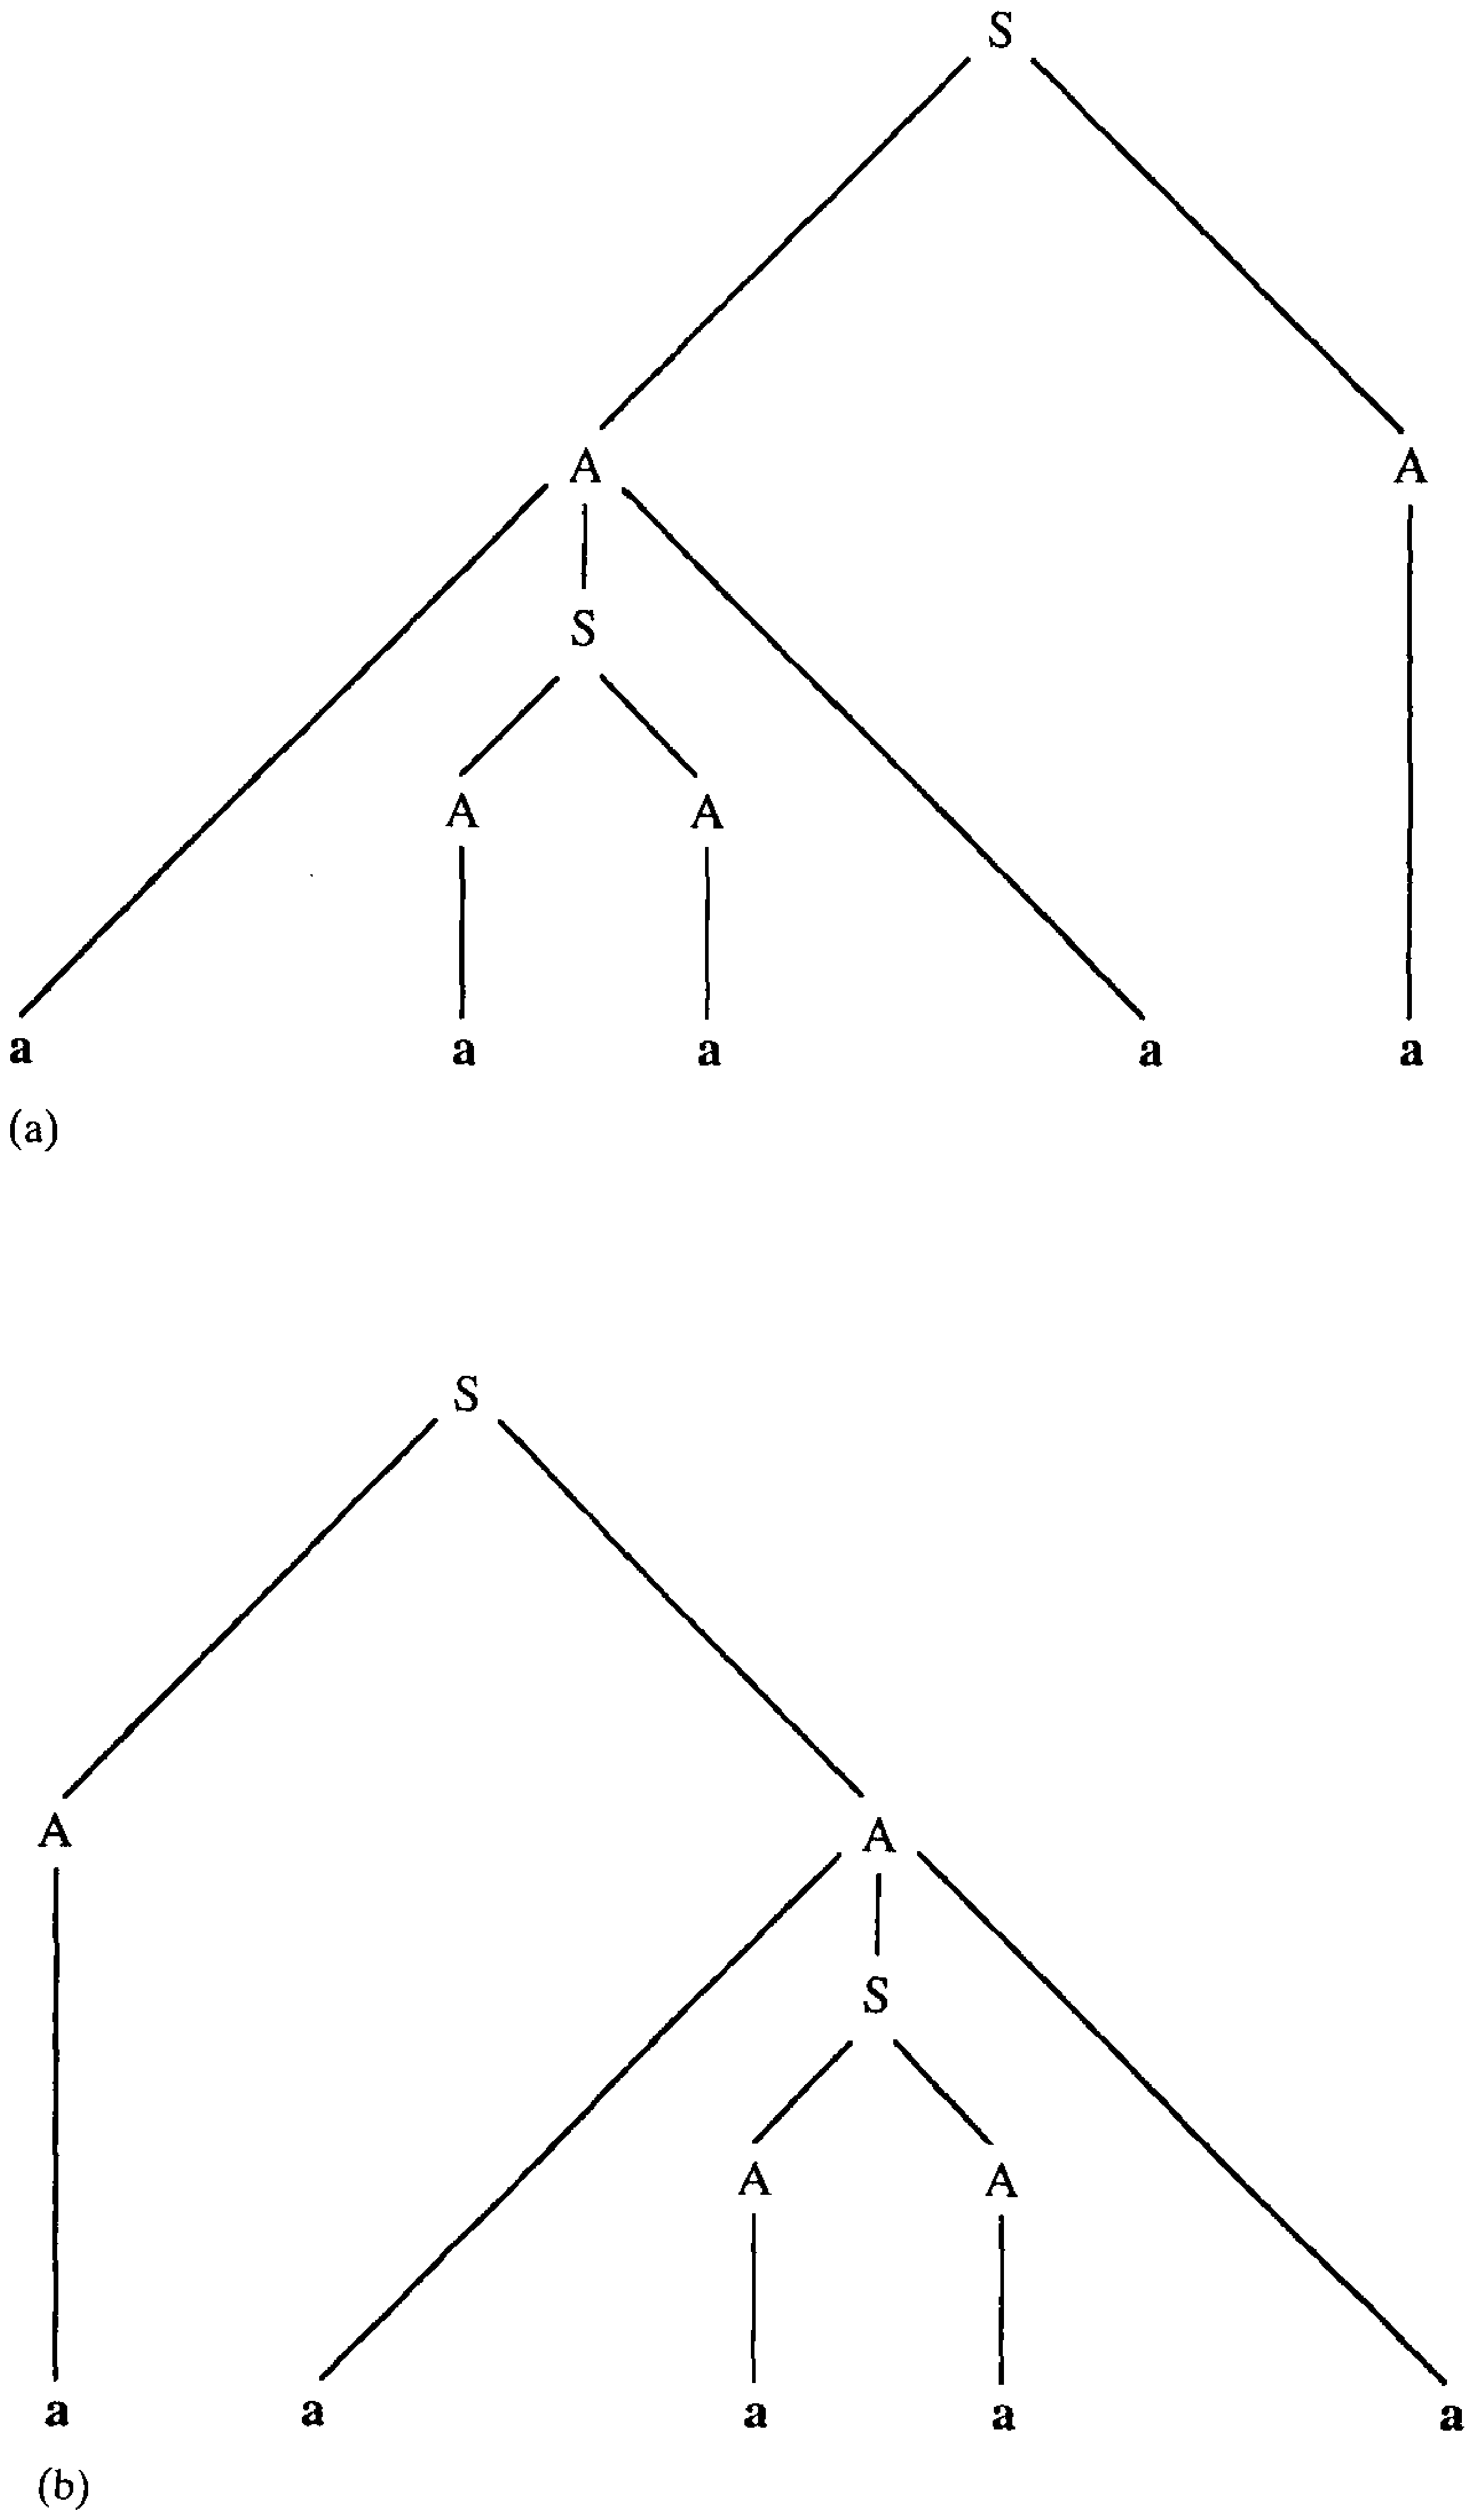
\epsfig{figure=ToFAfigures/fig9-5.eps,height=5.5in}}
\caption{(a) A parse tree for $\bf{aaaaa}$ in Example 9.5 (b) An alternate parse tree
for $\pmb{aaaaa}$}\label{fig-9.5}
\end{figure}

The following sampling from a potential programming language grammar illustrates
the semantic problems that can be caused by ambiguity. Consider the grammar
$G_s=\langle\{<$expression$>,<$identifier$>\},\{\pmb{a},\pmb{b},\\\pmb{c},\pmb{d},
\pmb{-}\},<$expression$>,P\rangle$, where $P$ consists of the productions
\begin{center}\begin{tabular}{r@{ $\rightarrow$ }l}
\<expression\> & \<identifier\> \\
\<expression\> & \<identifier\> -- \<expression\> \\
\<expression\> & \<expression\> -- \<identifier\> \\
\<identifier\> & $\pmb{a}$ \\
\<identifier\> & $\pmb{b}$ \\
\<identifier\> & $\pmb{c}$ \\
\<identifier\> & $\pmb{d}$
\end{tabular}\end{center}
$L(G_s)$ then contains the string $\pmb{a-b-d}$, which can be generated by
two distinct parse trees, as shown in Figure \ref{fig-9.6}. Figure \ref{fig-9.6}a corresponds to the
following leftmost derivation.
\begin{center}\begin{tabular}{r@{ $\Rightarrow$ }l}
\<expression\> & \<expression\> -- \<identifier\> \\
& \<identifier\> -- \<expression\> -- \<identifier> \\
& $\pmb{a-}$ \<expression\> -- \<identifier\> \\
& $\pmb{a-}$ \<identifier\> -- \<identifier\> \\
& $\pmb{a-b-}$ \<identifier\> \\
& $\pmb{a-b-d}$
\end{tabular}\end{center}
Figure \ref{fig-9.6}b corresponds to a different leftmost derivation, as shown below.
\begin{center}\begin{tabular}{r@{ $\Rightarrow$ }l}
\<expression\> & \<identifier\> -- \<expression\> \\
& $\pmb{a-}$ \<expression\> \\
& $\pmb{a-}$ \<identifier\> -- \<expression\> \\
& $\pmb{a-b-}$ \<expression\> \\
& $\pmb{a-b-}$ \<identifier\> \\
& $\pmb{a-b-d}$
\end{tabular}\end{center}
If the productions of $G_s$ were part of a grammatical description of a
programming language, there are obvious semantics associated with the
productions involving the $\pmb{-}$ operator. The productions
\[ \text{\<expression\>}\rightarrow\text{\<identifier\>}-\text{\<expression\>}\]
and
\[ \text{\<expression\>}\rightarrow\text{\<expression\>}-\text{\<identifier\>}\]
indicate that two values should be combined using the subtraction operator to
form a new value. The compiler would be responsible for generating code that
carried out the appropriate subtraction. Unfortunately, the two parse trees give
rise to functionally different code. For the parse tree in Figure \ref{fig-9.6}a, the
subtraction will be performed left to right, while in the parse tree in Figure
\ref{fig-9.6}b the ordering of the operators is right to left. Subtraction is \emph{not} a
commutative operation, and the expression $(a-b)-d$ will usually produce a
different value than $a-(b-d)$. Ambiguity can thus be a fatal flaw in a grammar
describing a programming language.

% Figure 9.6
\begin{figure}
\centerline{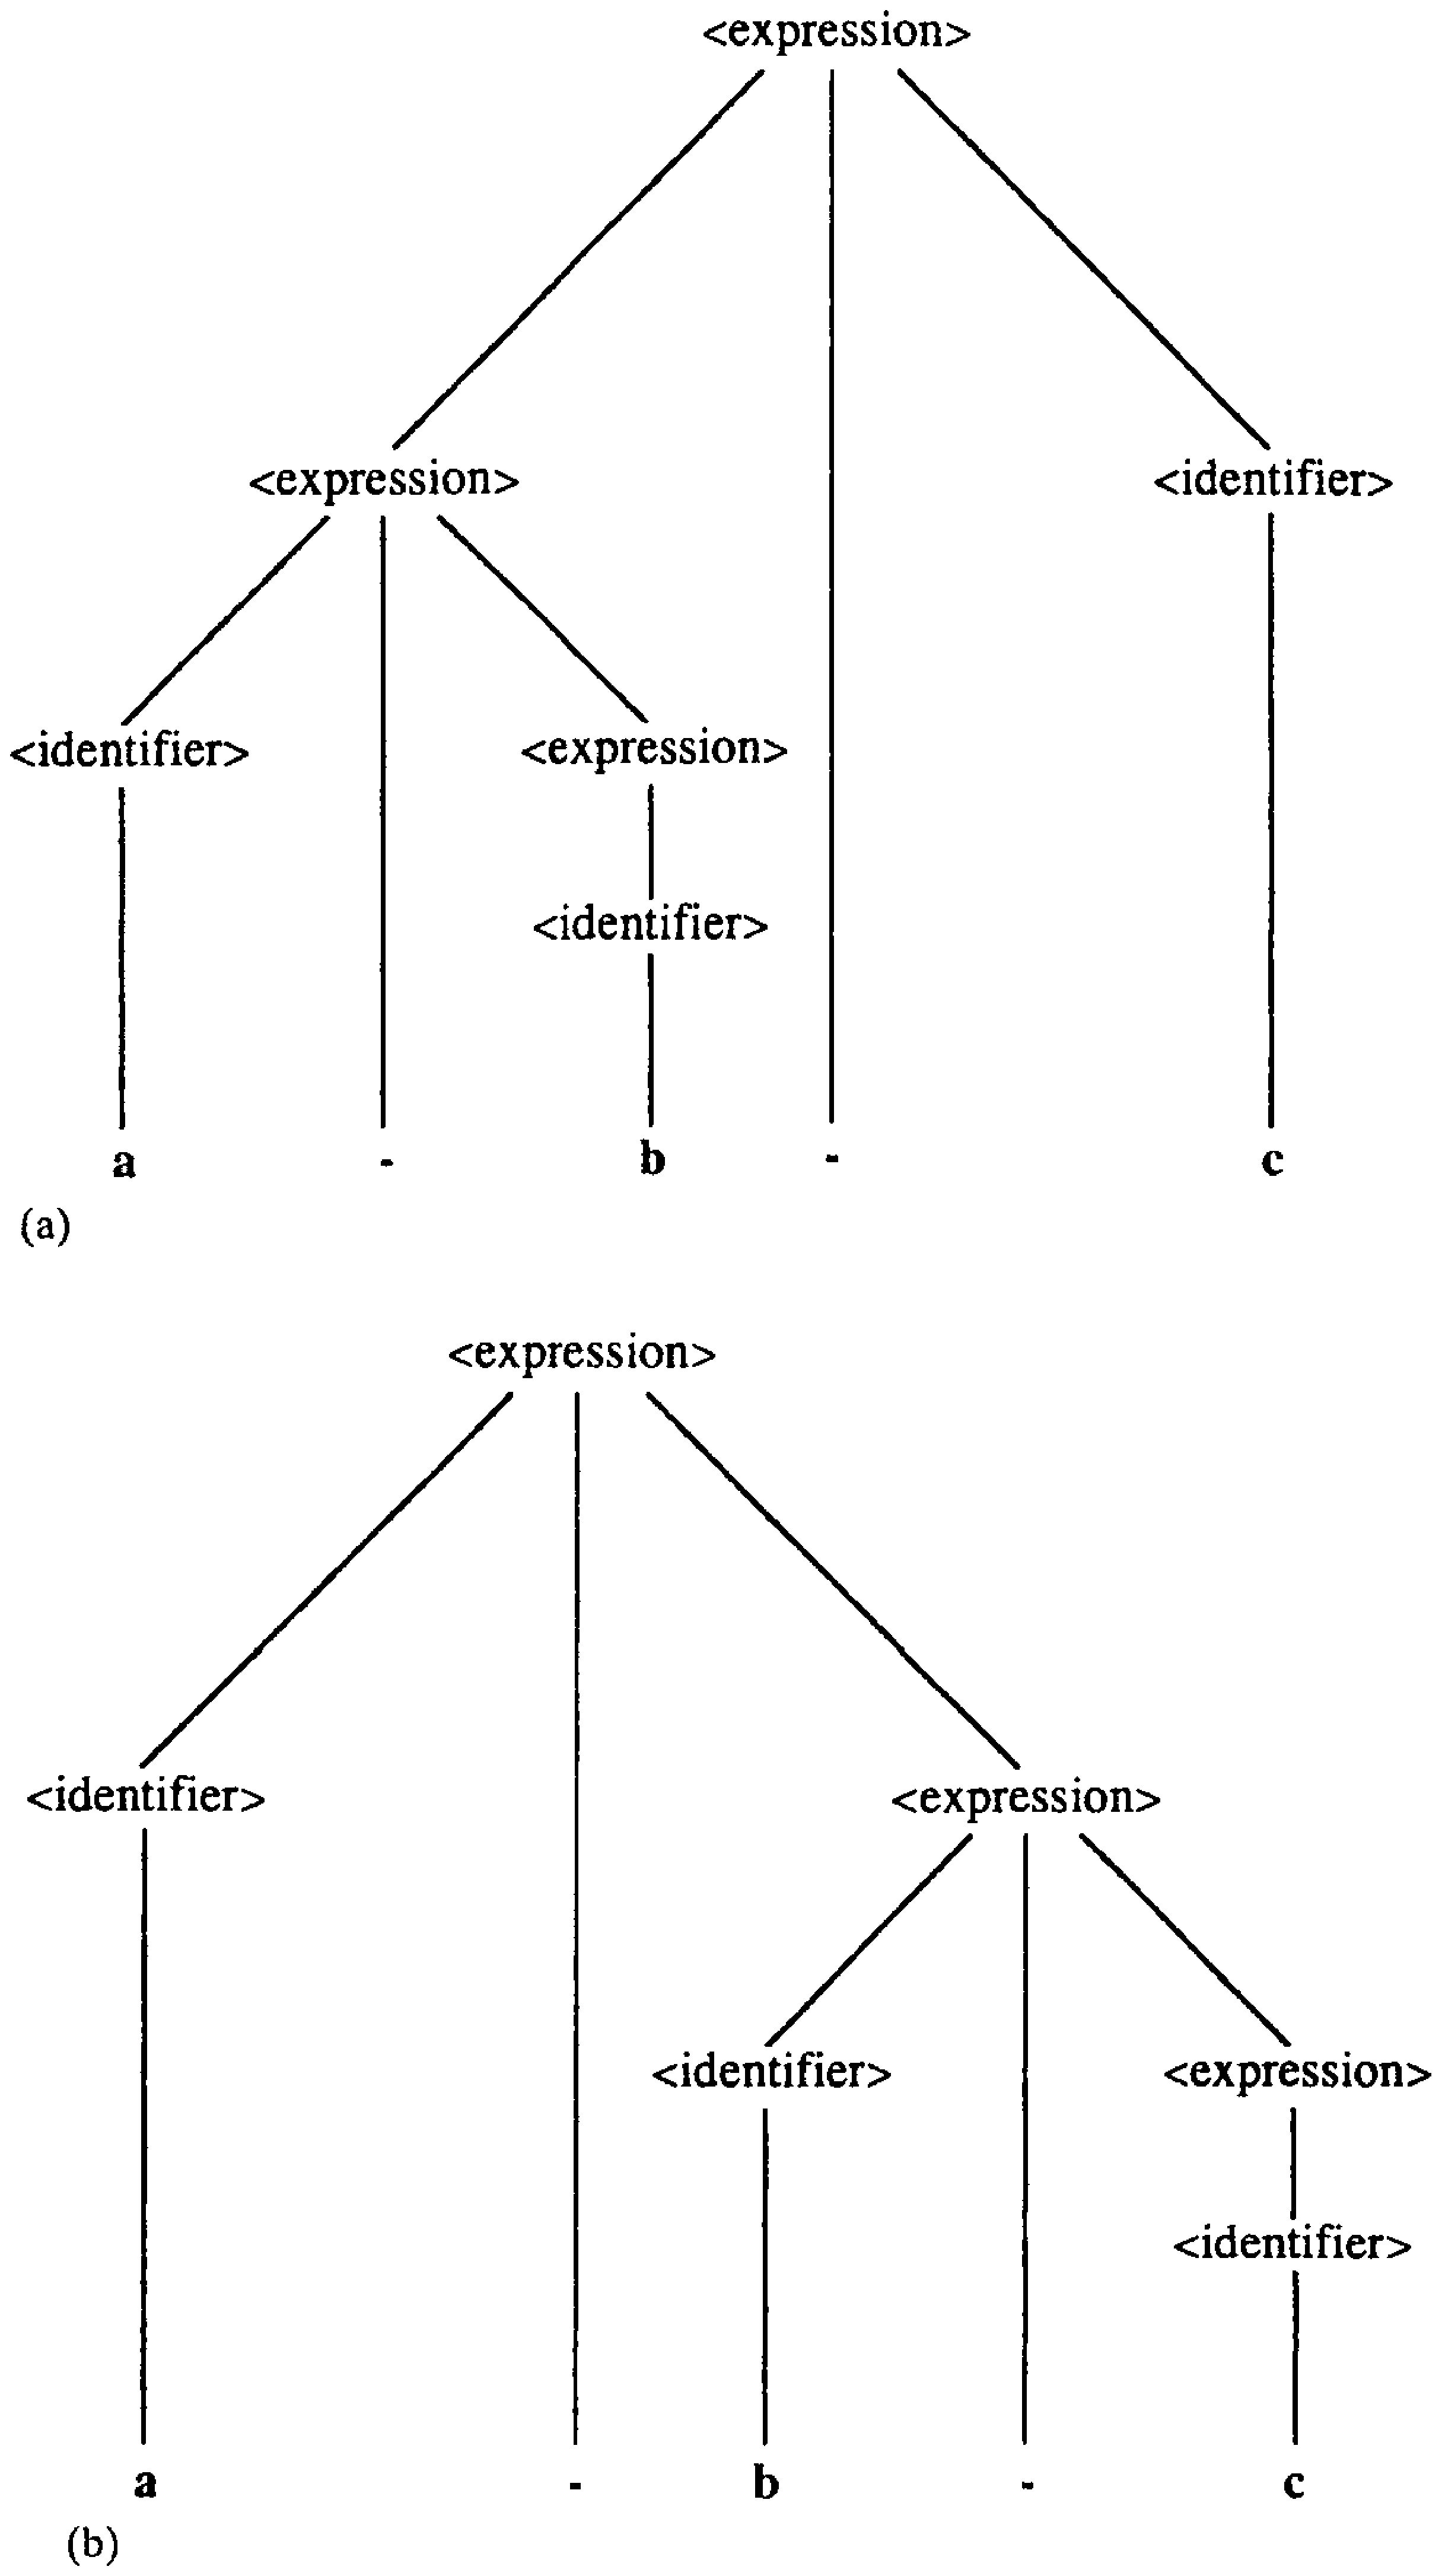
\epsfig{figure=ToFAfigures/fig9-6.eps,height=6.5in}}
\caption{(a) A parse tree for $\pmb{a-b-d}$ in Example 9.6 (b) An alternate
parse tree for $\pmb{a-b-d}$}\label{fig-9.6}
\end{figure}

In the language $L(G_s)$ discussed in Example 9.6, the ambiguity is again not
inherent in the language itself, but is rather a consequence of the specific
productions in the grammar $G_s$ describing the language. In most programming
languages, the expression $\pmb{a-b-d}$ is allowed and has a well-defined
meaning. Most languages decree that such expressions be evaluated from left to
right, and hence $\pmb{a-b-d}$ would be interpreted as ($\pmb{a-b}$)$\pmb{-d}$.
This interpretation can be enforced by simply removing the production
\[ \text{\<expression\>}\rightarrow\text{\<identifier\>}-\text{\<expression\>}\]
from $G_s$ to form the new grammar
\[ G_m = \langle\{\text{\<expression\>},\text{\<identifier\>}\},\{\pmb{a},\pmb{b},
	\pmb{c},\pmb{d},\pmb{-}\},\text{\<expression\>},P'\rangle \]
where $P'$ consists of the productions
\begin{center}\begin{tabular}{r@{ $\rightarrow$ }l}
\<expression\> & \<identifier\> \\
\<expression\> & \<expression\> -- \<identifier\> \\
\<identifier\> & $\pmb{a}$ \\
\<identifier\> & $\pmb{b}$ \\
\<identifier\> & $\pmb{c}$ \\
\<identifier\> & $\pmb{d}$
\end{tabular}\end{center}

It should be clear that $G_s$ and $G_m$ are equivalent, and both generate the
regular language $((\pmb{a}\cup\pmb{b}\cup\pmb{c}\cup\pmb{d})\cdot\pmb{-})^*
\cdot(\pmb{a}\cup\pmb{b}\cup\pmb{c}\cup\pmb{d})$. $G_m$ gives rise to unique
parse trees and is therefore unambiguous. It should be noted that the language
could have been defined with a single nonterminal; a simpler grammar equivalent
to $G_m$ is $G_t = \langle\{T\},\{\pmb{a},\pmb{b},\pmb{c},\pmb{d},\pmb{-}\},T,\{
T\rightarrow\pmb{a}|\pmb{b}|\pmb{c}|\pmb{d}|T - T\}\rangle$. However, since
$G_t$ is ambiguous, it is much more difficult to work with than $G_m$. The pair
of nonterminals \<expression\> and \<identifier\> are used to circumvent the
ambiguity problem in this language. For the grammar $G_m$, the production
\[ \text{\<expression\>}\rightarrow\text{\<expression\>}-\text{\<identifier\>}\]
contains the nonterminal \<expression\> to the left of the subtraction token and
\<identifier\> to the right of the $\pmb{-}$. Since \<identifier\> can only be
replaced by a terminal representing a single variable, the resulting parse tree
will ensure that the entire expression to the left of the $\pmb{-}$ will be
evaluated before the operation corresponding to this current subtraction token
is performed. In this fashion, the distinction between the two nonterminals
forces a left-to-right evaluation sequence. In fact, a more robust language with
other operators like $\times$ and $\div$ will require more nonterminals to
enforce the default precedence among these operators.

Most modern programming languages employ a solution to the ambiguity problem
that is different from the one just described. Programmers generally do not
want to be constrained by operators that can only be evaluated from left to
right, and hence matched parentheses are used to indicate an order of evaluation
that may differ from the default. Thus, unambiguous grammars that correctly
reflect the meaning of expressions like $d-(b-c)$ or even $(a)-((c-(d)))$ are
sought.

\subsection*{Example 9.7}

The following grammar $G_P$ allows expressions with parentheses, minus signs,
and single-letter identifiers to be uniquely parsed.
\[ G_P = \langle\{\text{\<expression\>},\text{\<identifier\>}\},\{\pmb{a},
	\pmb{b},\pmb{c},\pmb{d},\pmb{-},\pmb{(},\pmb{)}\},\text{\<expression\>},
	P''\rangle \]
where $P''$ consists of the productions
\begin{center}\begin{tabular}{r@{ $\rightarrow$ }l}
\<expression\> & (\<expression\>) \\
\<expression\> & \<expression\> -- (\<expression\>) \\
\<expression\> & \<identifier\> \\
\<expression\> & \<expression\> -- \<identifier\> \\
\<identifier\> & $\pmb{a}$ \\
\<identifier\> & $\pmb{b}$ \\
\<identifier\> & $\pmb{c}$ \\
\<identifier\> & $\pmb{d}$
\end{tabular}\end{center}

The first two productions in $P''$, which were not present in $P'$, are designed
to handle the balancing of parentheses. The first rule allows superfluous sets
of parentheses to be correctly recognized. The second rule ensures that an
expression that is surrounded by parentheses is evaluated before the operator
outside those parentheses is evaluated. In the absence of parentheses, the
left-to-right ordering of the operators is maintained. Figure \ref{fig-9.7} illustrates
the unique parse tree for the expression $(a)-((c-(d)))$.

$G_P$ is a context-free language that is too complex to be regular; the pumping
lemma for regular sets (Theorem \ref{thm-2.3}) can be used to show that is impossible for
a DFA to maintain an unlimited number of corresponding balanced parentheses.
This language, and the others discussed so far, can all be expressed by
unambiguous grammars. It should be clear that \emph{every} language generated by
grammars has ambiguous grammars that also generate it, since an unambiguous
grammar can always be modified to become ambiguous. What is not immediately
clear is whether there are languages that can \emph{only} be generated by
ambiguous grammars.

% Definition 9.5
\begin{dfn}\label{dfn-9.5}\index{unambiguous context free grammar}\index{inherently ambiguous}\index{language!inherently ambiguous}\index{language!unambiguous}
A context-free language $L$ is called \emph{inherently ambiguous} if
every grammar that generates $L$ is ambiguous. A context-free language that is
not inherently ambiguous is called \emph{unambiguous}.
\end{dfn}

% Definition 9.6
\begin{dfn}\label{dfn}\index{C@\CSIG \ (C-sigma)}\index{U@\USIG \ (U-sigma )}
Let the class of context-free language $L$ over the alphabet $\Sigma$ be denoted
by \CSIG. Let the class of unambiguous context-free languages be denoted by
\USIG
\end{dfn}

% Theorem 9.1
\begin{thm}\label{thm-9.1}\index{ambiguous context free language, inherently}\index{inherently ambiguous}
There are context-free languages that are inherently ambiguous; that is, \USIG\ 
is properly contained in \CSIG.

\emph{Proof.} The language $L=\{\pmb{a}^n\pmb{b}^n\pmb{c}^m\pmb{d}^m|n,m\in\NN\}
\cup\{\pmb{a}^i\pmb{b}^j\pmb{c}^j\pmb{d}^i|i,j\in\NN\}$ is a context-free
language (see the exercises). $L$ is also inherently ambiguous, since there must
exist two parse trees for some of the strings in the intersection of the two
sets $\{\pmb{a}^n\pmb{b}^n\pmb{c}^m\pmb{d}^m|n,m\in\NN\}$ and $\{\pmb{a}^i\pmb{b}
^j\pmb{c}^j\pmb{d}^i|i,j\in\NN\}$. The proof of this last statement is
tedious to formalize; the interested reader is referred to [HOPC].
\end{thm}

% Figure 9.7
\begin{figure}
\centerline{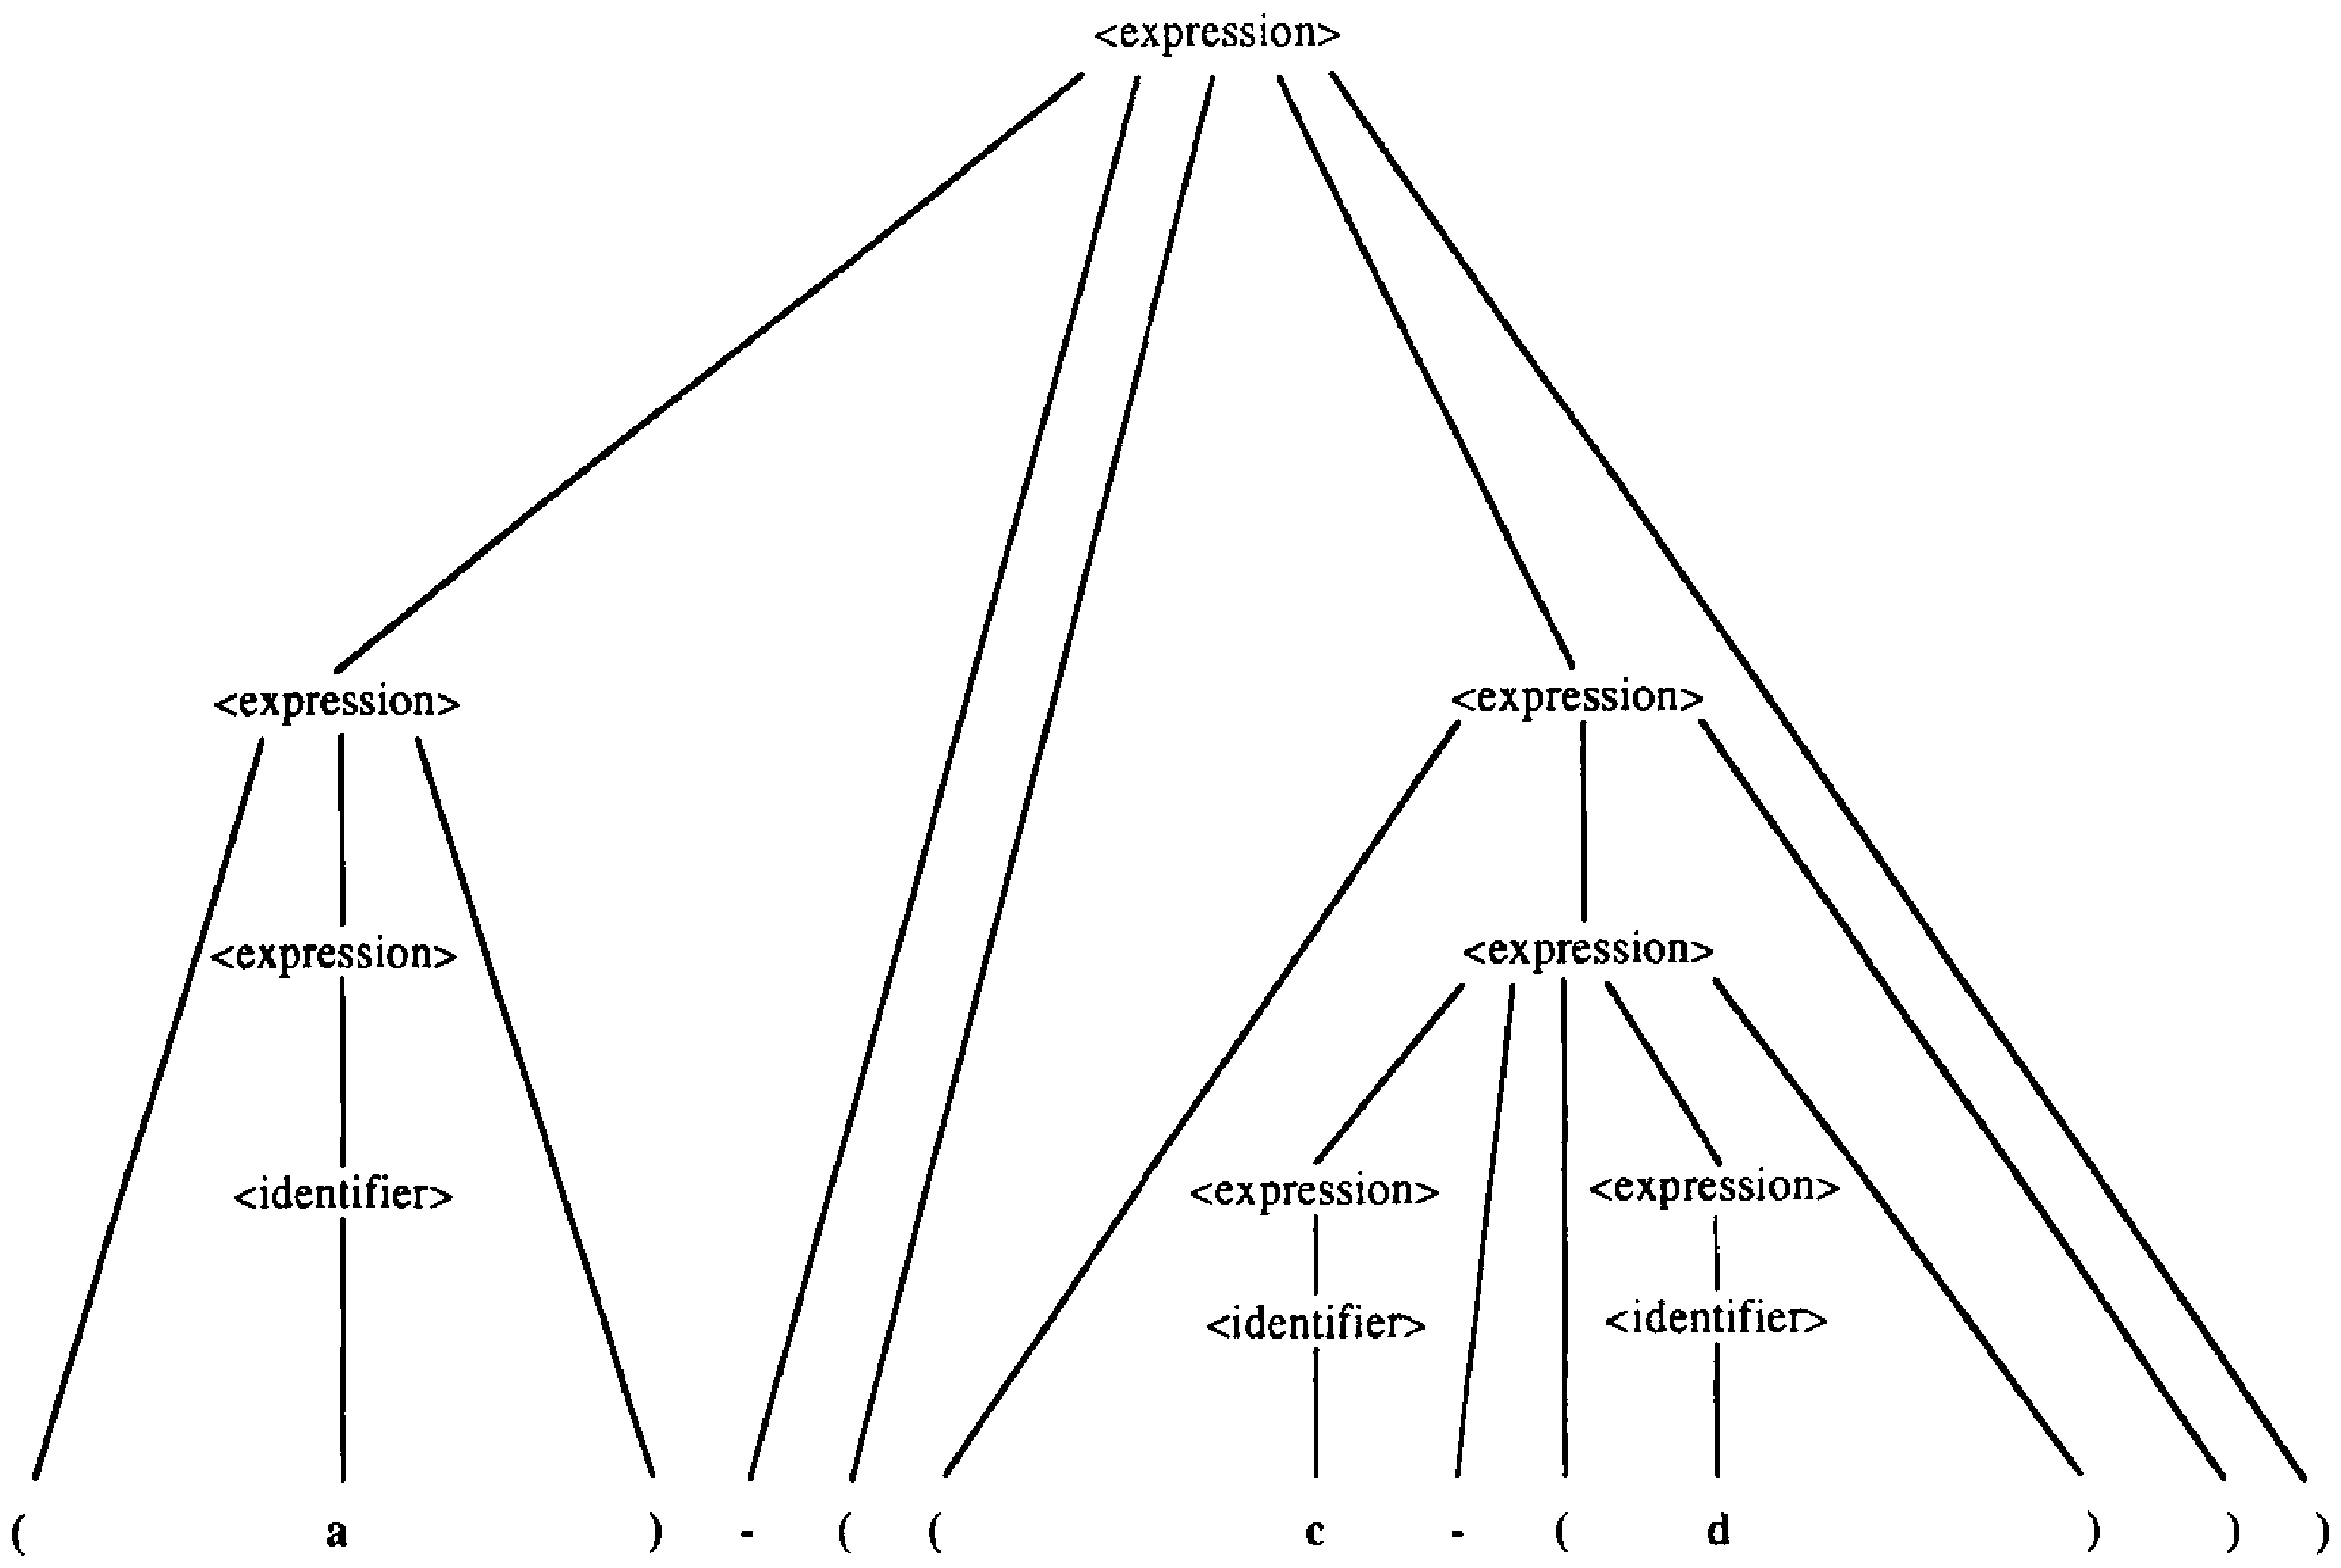
\epsfig{figure=ToFAfigures/fig9-7.eps,height=3.5in}}
\caption{The parse tree discussed in Example 9.7}\label{fig-9.7}
\end{figure}

Theorem \ref{thm-9.1} states that there exist inherently ambiguous type 2 languages. No
type 3 language is inherently ambiguous. Even though there are regular grammars
that are ambiguous, every regular grammar has an equivalent grammar that is
unambiguous. This assertion is supported by the following examples and
results.

\subsection*{Example 9.8}

Consider the following right-linear grammar $G_r$:
\[ G_r = \langle\{S,A,C\},\{\pmb{a},\pmb{b},\pmb{c}\},S,\{S\rightarrow A\pmb{bc},
	S\rightarrow\pmb{ab}C,A\rightarrow\pmb{a},C\rightarrow\pmb{c}\}\rangle \]
Only one terminal string can be derived from $G_r$, but this word has two
distinct derivation trees, as shown in Figure \ref{fig-9.8}. Thus, there are regular
grammars that are ambiguous.

% Theorem 9.2
\begin{thm}\label{thm-9.2}
Given any right-linear grammar\ \,$G=\langle\Omega,\Sigma,S,P\rangle$, there exists
an equivalent right-linear grammar that is unambiguous.

\emph{Proof.} Let $G'=G_{(A^{\sigma d}_G)}$. That is, beginning with the
right-linear grammar G, use the construction outlined in Lemma \ref{lmm-8.2} to find the
corresponding automaton $A_G$. Use Definition \ref{dfn-4.9} to remove the
lambda-transitions and Definition \ref{dfn-4.5} to produce a deterministic machine, and
then apply the construction outlined in Lemma \ref{lmm-8.1} to form the new right-linear
grammar $G'$. By Lemma \ref{lmm-8.2}, Theorem \ref{thm-4.2}, Theorem \ref{thm-4.1}, and Lemma \ref{lmm-8.1}, the
language defined by each of these constructs is unchanged, so $G'$ is equivalent
to $G$. Due to the deterministic nature of the machine from which this new
grammar was built, the resulting parse tree for a given string must be unique,
since only one production is applicable at any point in the derivation. A formal
inductive statement of this property is left as an exercise.
\end{thm}

% Figure 9.8
\begin{figure}
\centerline{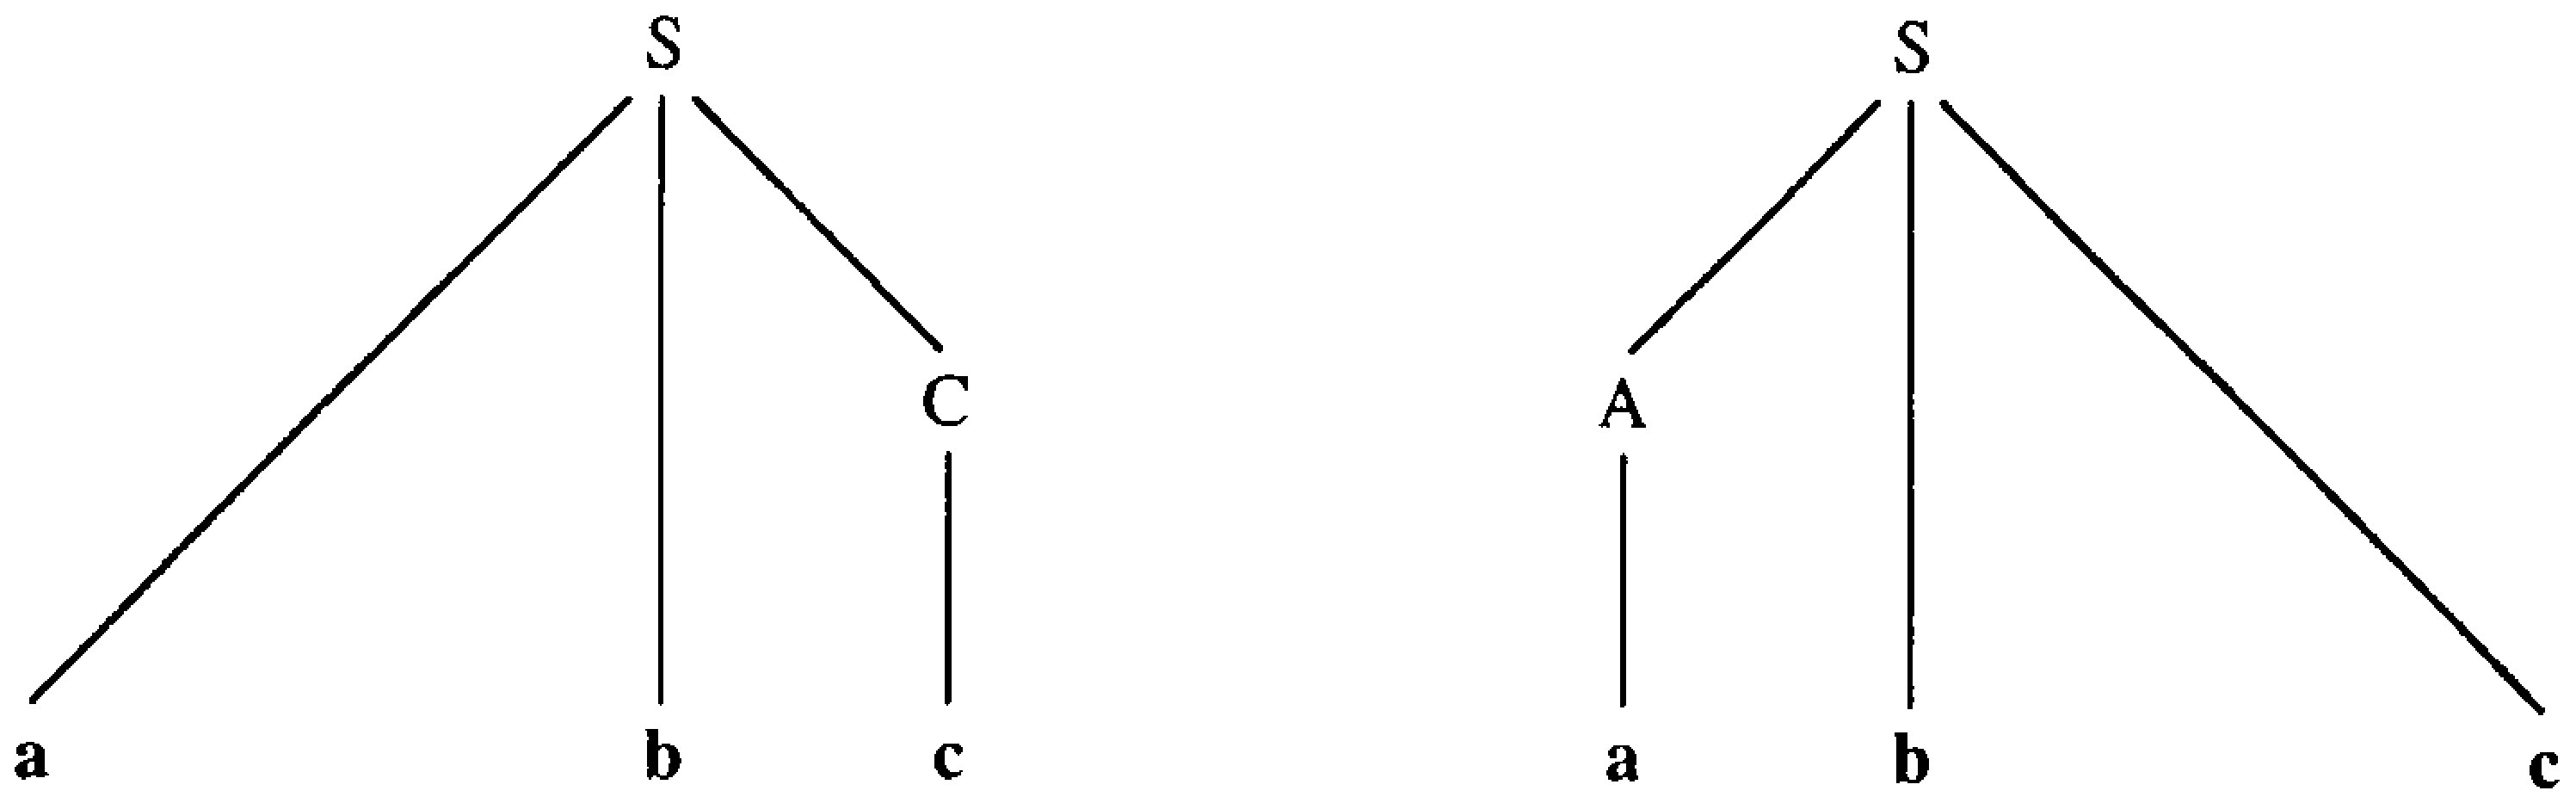
\epsfig{figure=ToFAfigures/fig9-8.eps,width=5.0in}}
\caption{The parse trees discussed in Example 9.8}\label{fig-9.8}
\end{figure}

% Corollary 9,1
\begin{cor}\label{cor-9.1}
The class \GSIG\ of languages generated by regular grammars is properly
contained in \USIG.

\emph{Proof.} Containment follows immediately from Theorem \ref{thm-9.2}. Proper
containment is demonstrated by the language and grammar discussed in Example 9.3.
\end{cor}

\subsection*{Example 9.9}

The right-linear grammar
\[ G_r = \langle\{S,B,C\},\{\pmb{a},\pmb{b},\pmb{c}\},S,\{S\rightarrow\pmb{a}B,
	S\rightarrow\pmb{ab}C,B\rightarrow\pmb{bc},C\rightarrow\pmb{c}\}\rangle \]
in Example 9.8 can be transformed, as outlined in Theorem \ref{thm-9.2}, into an
unambiguous grammar. The automaton corresponding to $G_r$ found by applying the
technique given in Lemma \ref{lmm-8.2} is shown in Figure \ref{fig-9.9}a. The version of this
automaton without lambda-moves (with the inaccessible states not shown) is
illustrated in Figure \ref{fig-9.9}b. The deterministic version, with the disconnected
states again removed, is given in Figure \ref{fig-9.9}c. For simplicity, the states are
relabeled in Figure \ref{fig-9.9}d. The corresponding grammar specified by Lemma \ref{lmm-8.1} is
\begin{center}\begin{tabular}{r@{ }l}
$G' =$ & $\langle\{S_0,S_1,S_2,S_3,S_4\},\{\pmb{a},\pmb{b},\pmb{c}\},S_0,\{S_0
	\rightarrow\pmb{a}S_1|\pmb{b}S_4|\pmb{c}S_4,S_1\rightarrow\pmb{a}S_4|
	\pmb{b}S_2|\pmb{c}S_4,$ \\
& $S_2\rightarrow\pmb{a}S_4|\pmb{b}S_4|\pmb{c}S_3,S_3\rightarrow\lambda|\pmb{a}
	S_4|\pmb{b}S_4|\pmb{c}S_4,S_4\rightarrow\pmb{a}S_4|\pmb{b}S_4|\pmb{c}S_4
	\}\rangle$
\end{tabular}\end{center}

% Figure 9.9
\begin{figure}
\centerline{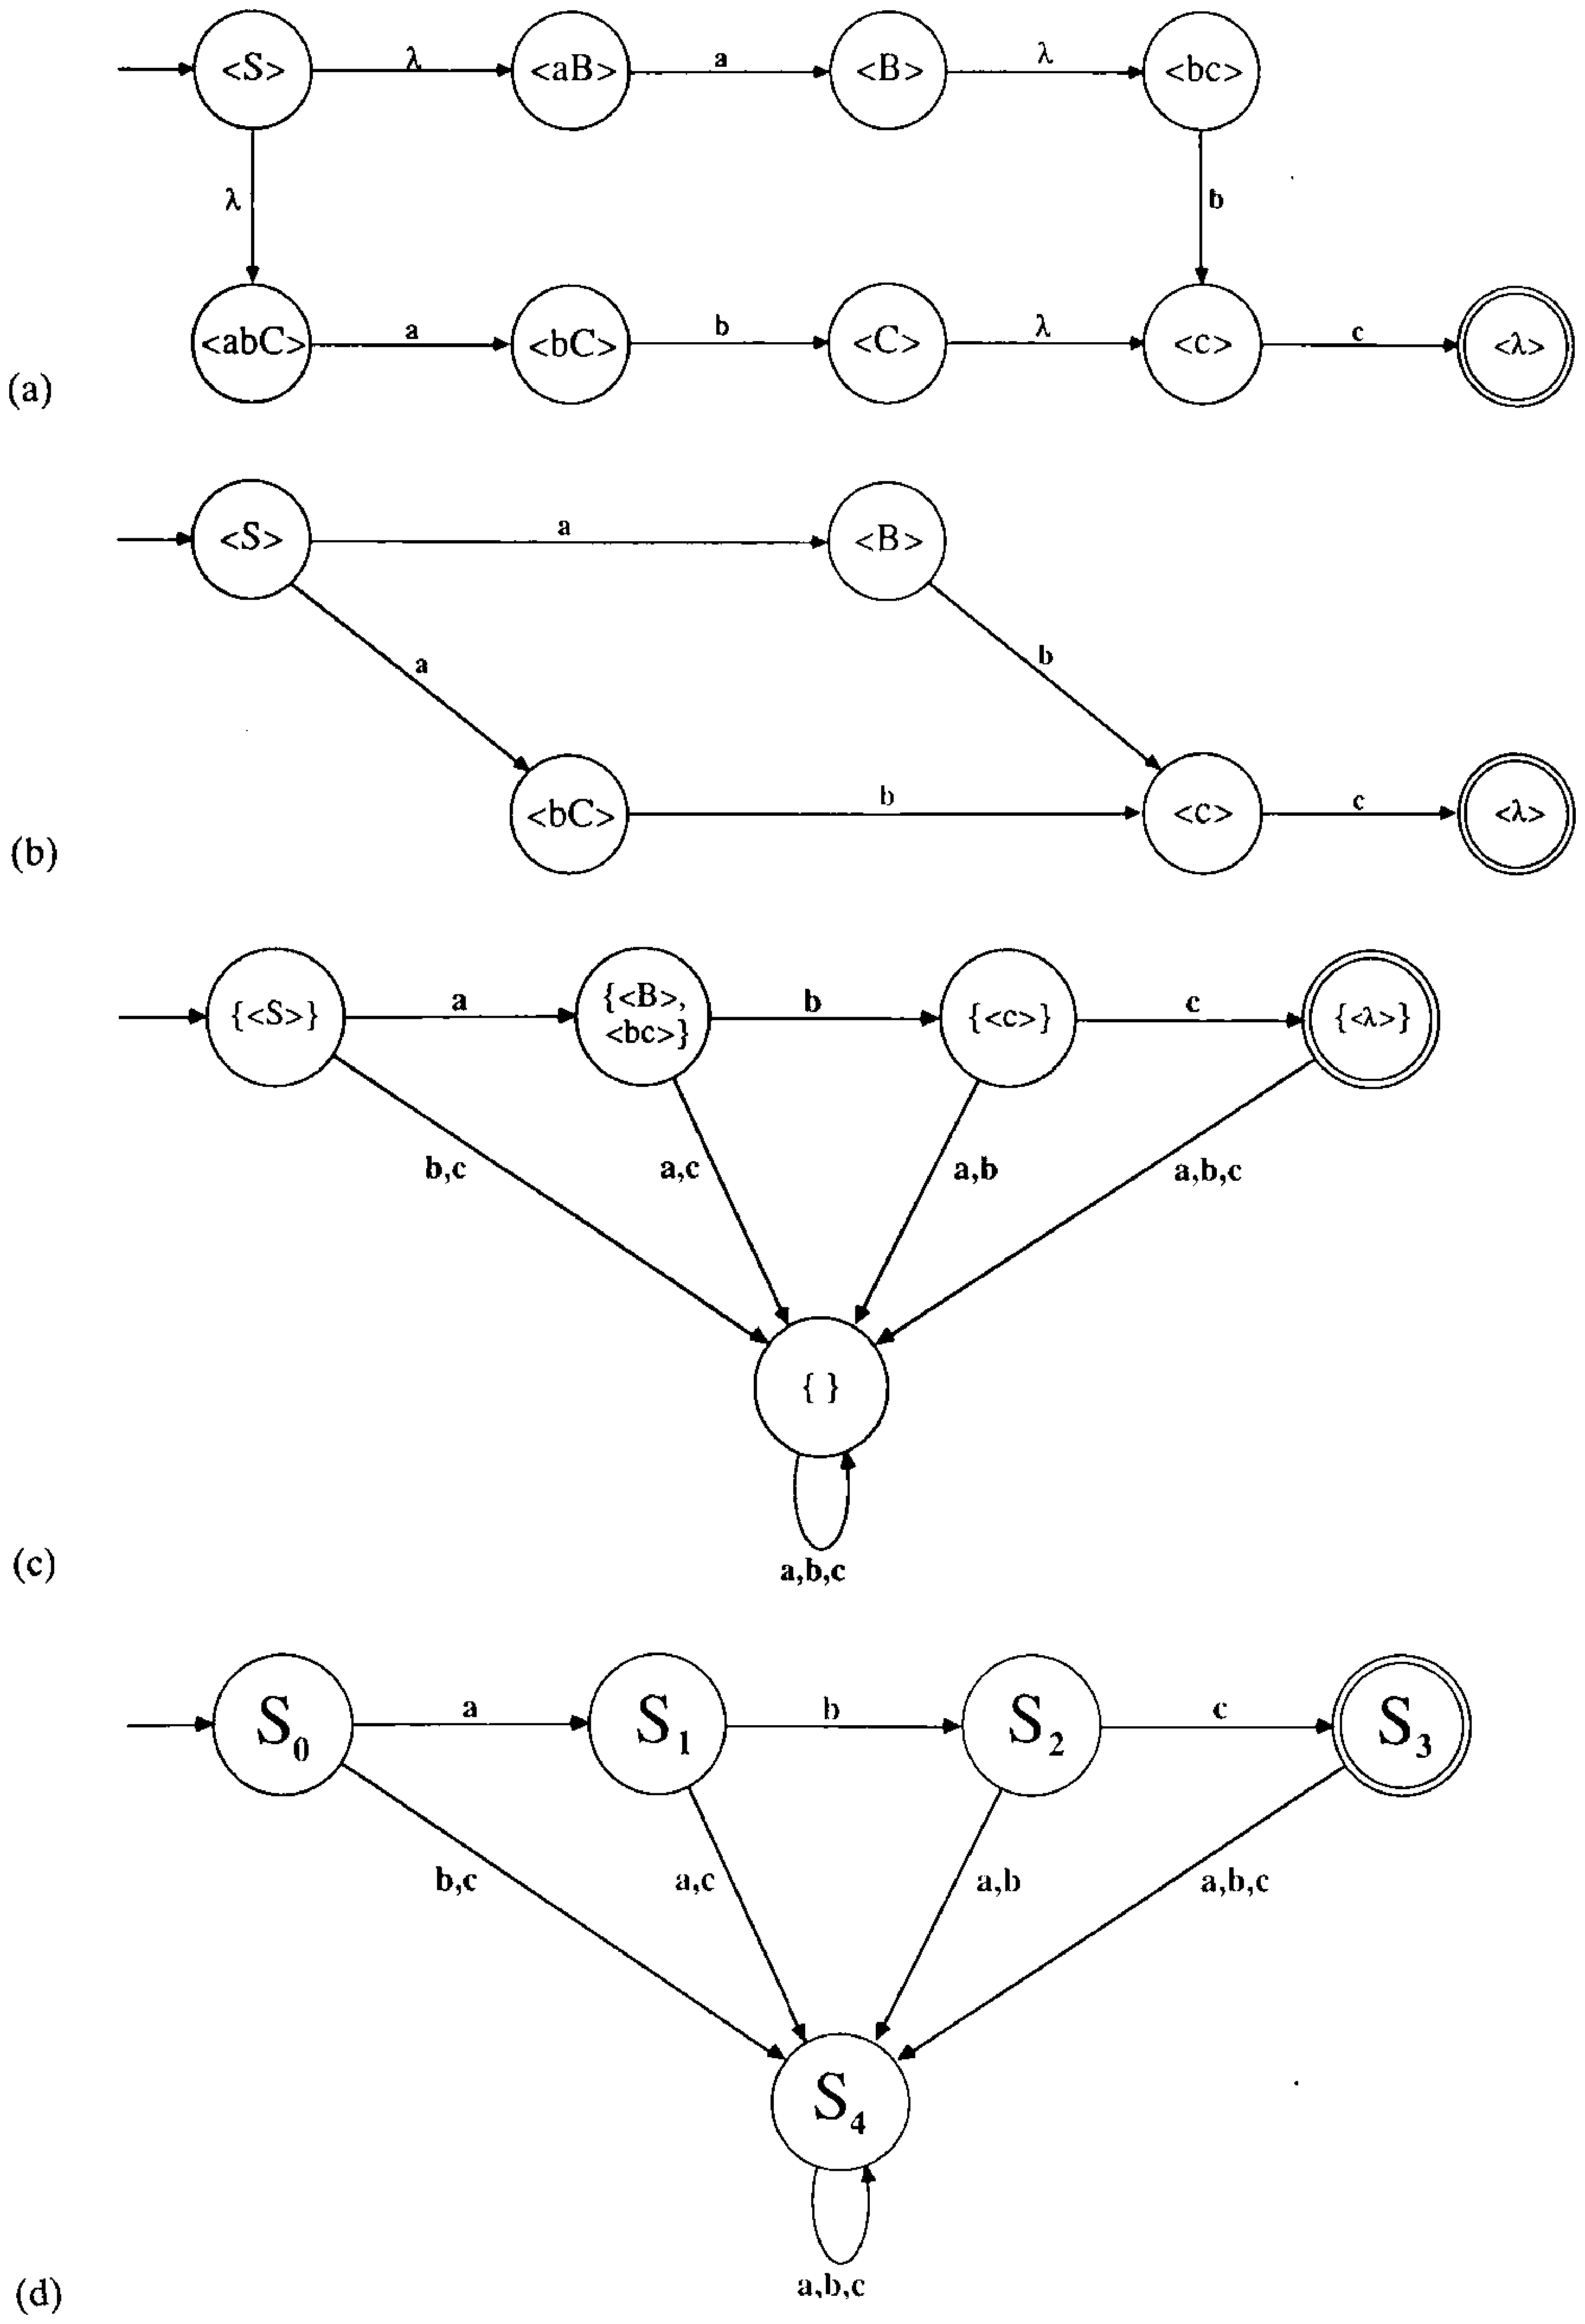
\epsfig{figure=ToFAfigures/fig9-9.eps,height=7.5in}}
\caption{(a) The automaton discussed in Example 9.9 (b) The simplified
automaton discussed in Example 9.9 (c) The deterministic automaton discussed
in Example 9.9 (d) The final automaton discussed in Example 9.9}\label{fig-9.9}
\end{figure}

The orderly nature of this resulting type of grammar easily admits the
specification of an algorithm that scans a proposed terminal string and builds
the corresponding parse tree. The partial parse tree for a string such as {\bf
abb} would be as pictured in Figure \ref{fig-9.10}a. This would clearly be an invalid
string since $S_4$ cannot be replaced by $\lambda$. By contrast, the tree for
the word $\pmb{abc}$ would produce a complete parse tree, and it is instructive to
step through the process by which it is built. The root of the tree must be
labeled $S_0$, and scanning the first letter of the word $\pmb{abc}$ is sufficient
to determine that the first production to be applied is $S_0\rightarrow\pmb{a}S_1$
(since no other $S_0$-rule immediately produces an $\pmb{a}$). Scanning the next
letter provides enough information to determine that the next $S_1$ rule that is
used must be $S_1\rightarrow\pmb{b}S_2$, and the third letter admits the
production $S_2\rightarrow\pmb{c}S_3$ and no other. Recognizing the end of the
string causes a check for whether the current non terminal can produce the empty
string. Since $S_3\rightarrow\lambda$ is in the grammar, the string $\pmb{abc}$ is
a valid terminal string, and corresponds to the parse tree shown in Figure \ref{fig-9.10}b.

% Figure 9.10
\begin{figure}
\centerline{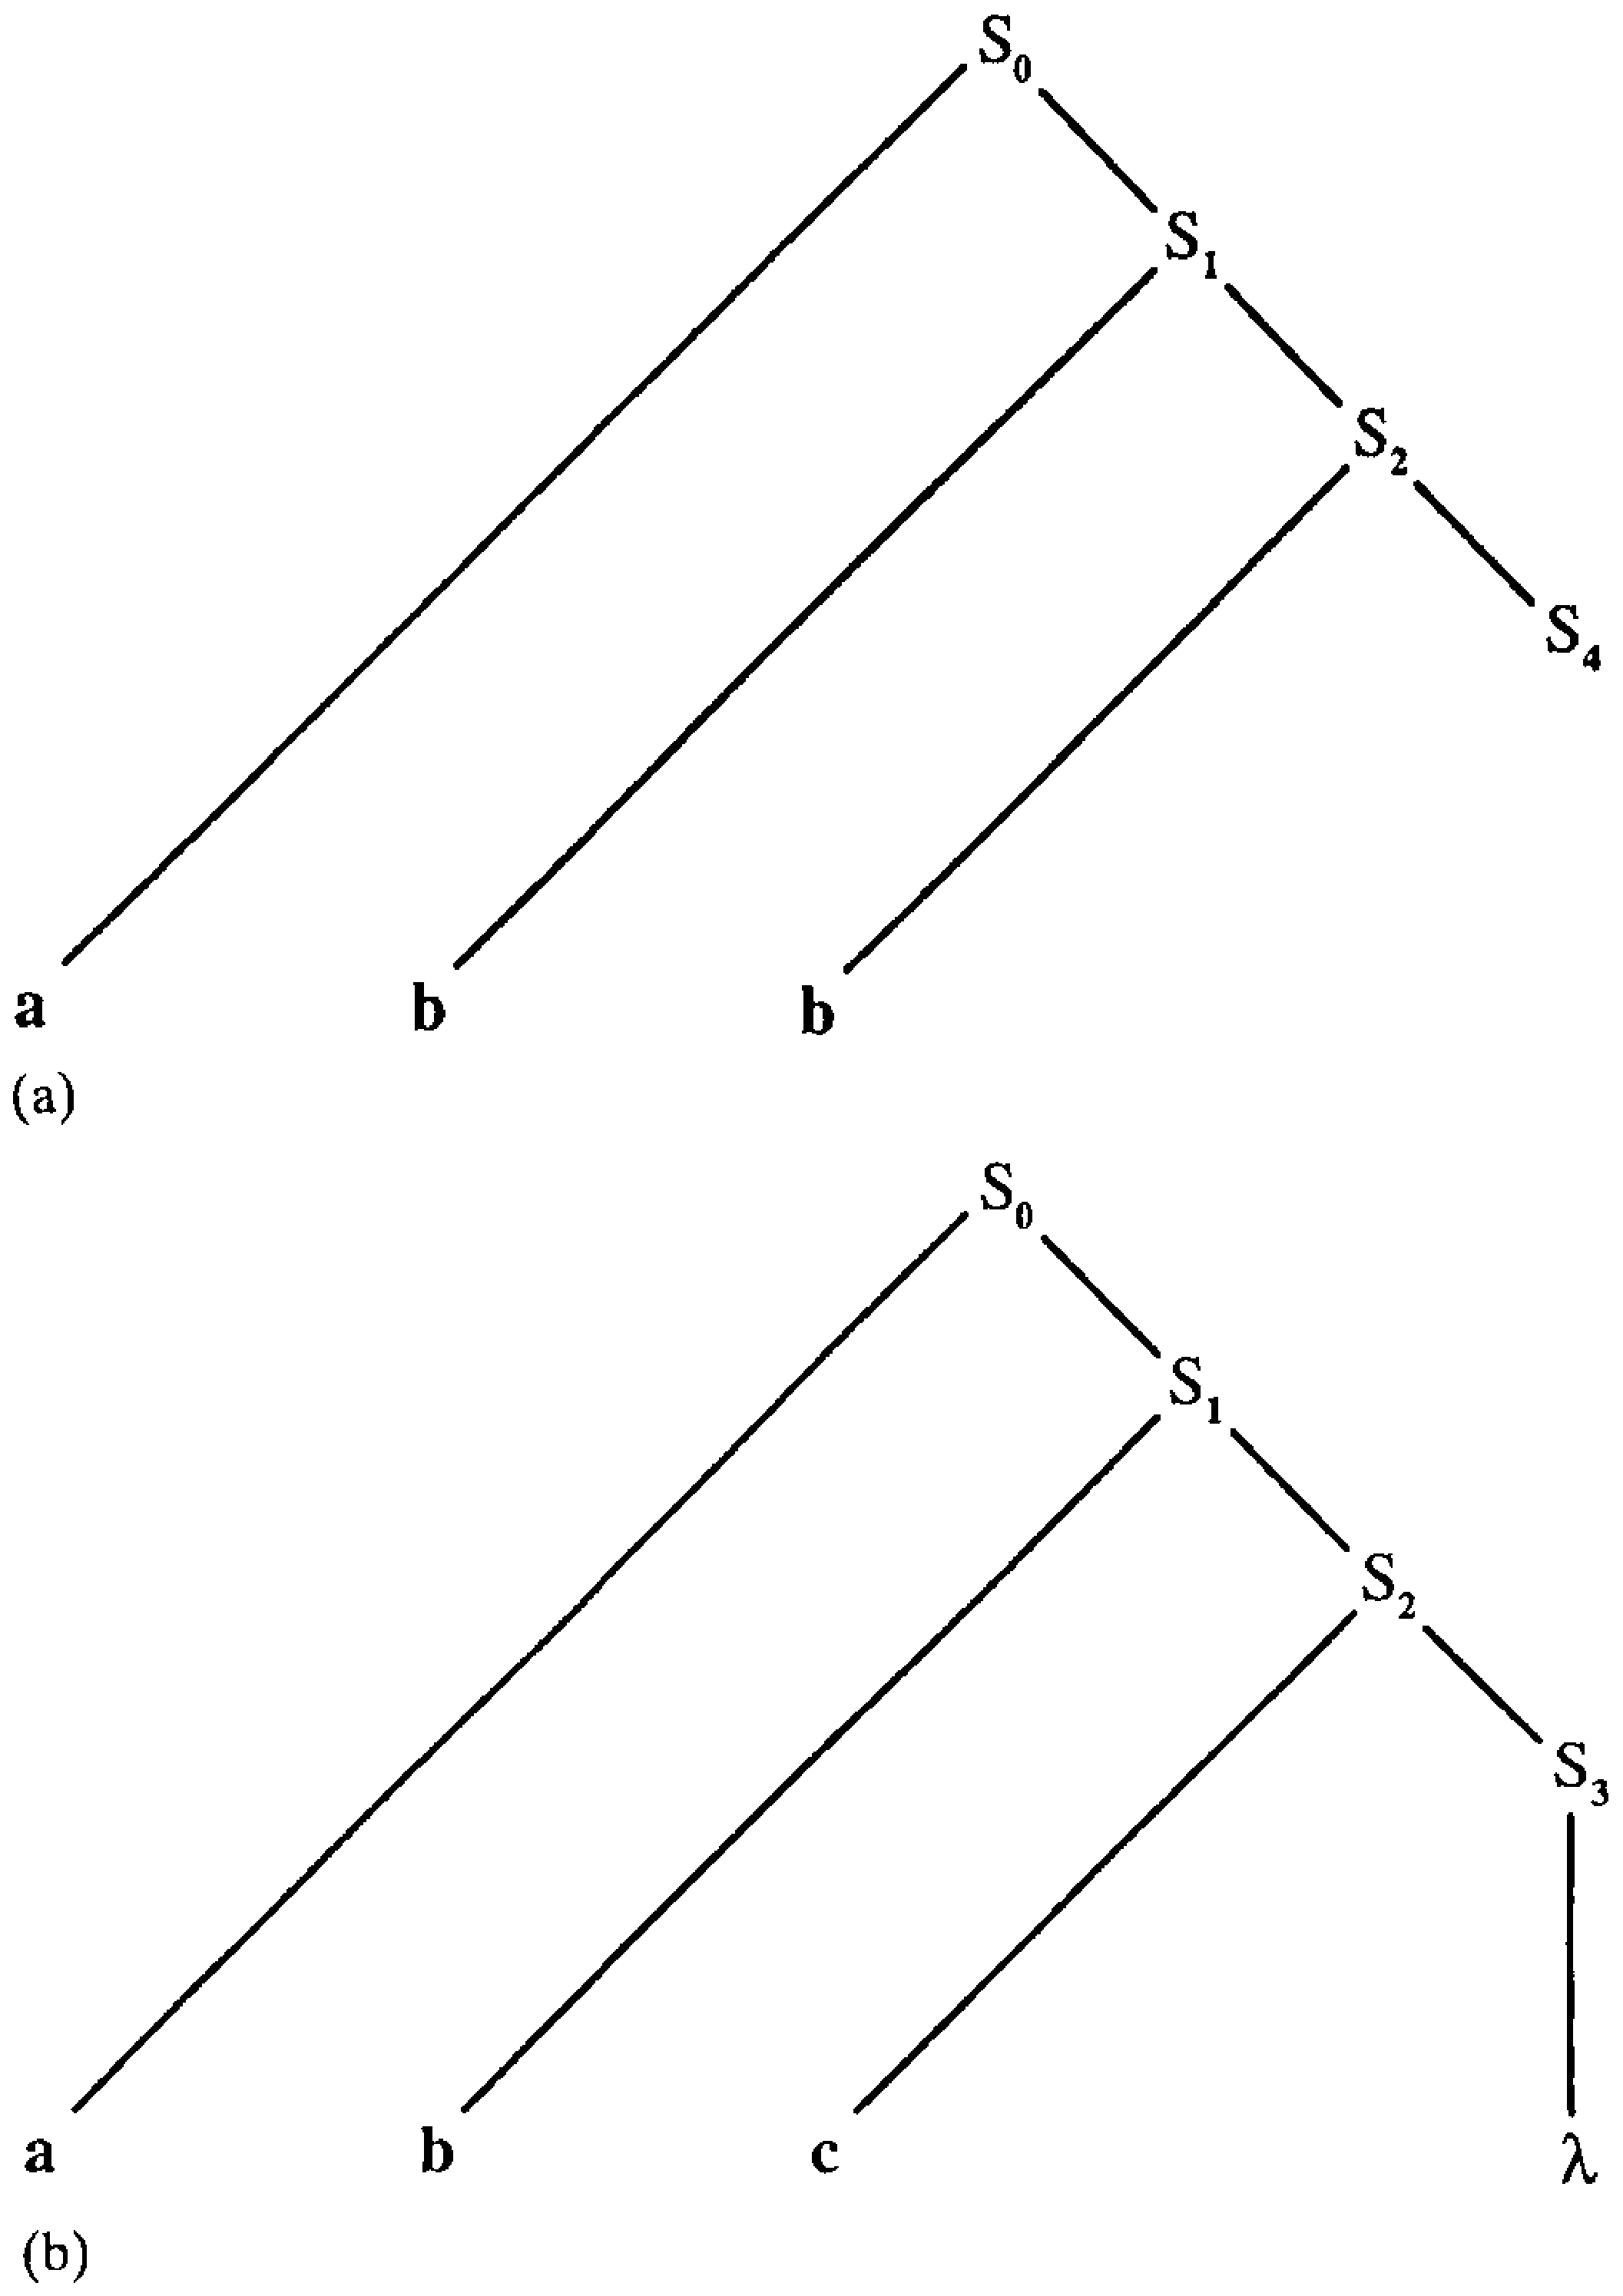
\epsfig{figure=ToFAfigures/fig9-10.eps,height=3.7in}}
\caption{(a) The partial parse tree for the string $\pmb{abb}$ (b) The parse tree
for the string $\pmb{abc}$}\label{fig-9.10}
\end{figure}

Grammars that admit scanning algorithms like the one outlined above are called
\Index{LL0} grammars since the parse tree can be deduced using a \underline{l}eft-to-right
scan of the proposed string while looking ahead \underline{0} symbols to produce
a \underline{l}eftmost derivation. That is, the production that produces a given
symbol can be immediately determined without regard to the symbols that follow.

Note that the grammar $G_3=\langle\{T\},\{\pmb{a}\},T,\{T\rightarrow\pmb{aaa}T,
T\rightarrow\pmb{aa}\}\rangle$ is LL2; that is, upon seeing $\pmb{a}$, the scanner
must look ahead two symbols to see if the end-of-string marker is imminent. In
this grammar, $\pmb{a}$ may be produced by either of the two $T$-rules; the
letters following this symbol in the proposed string are an important factor in
determining which production must be applied. The language described by $G_3$ is
simple enough to be defined by a grammar that is LL0, since every regular
grammar can be transformed as suggested by the proof of Theorem \ref{thm-9.2}.

The deterministic orderliness of LL0 grammars may be generally unattainable,
but it represents a desirable goal that a compiler designer would strive to
approximate when specifying a grammatical model of a programming language.
When a grammar is being defined to serve as a guide to construct a compiler,
an LL0 grammar is clearly the grammar of choice. Indeed, if even a portion of a
context-free grammar conforms to the LL0 property, this is of considerable
benefit. Whereas the technique outlined in Theorem \ref{thm-9.2} could be applied to any
regular language to find a hospitable LL0 grammar, programming languages are
generally more complex than regular languages, and these languages are unlikely
to have LL0 models. For context-free languages, it is much more likely that it
will not be possible to immediately determine which production (or sequence of productions)
will produce the symbol currently being scanned. In such cases, it will be
necessary to look ahead to successive symbols to make this determination.

A classic example of the need to look ahead in parsing programming languages
is reflected in the following FORTRAN statement:
\[ \mathtt{DO\ 77\ I=\ 1.5} \]\index{DO loop lookahead}
Since FORTRAN allows blanks within identifiers, this is a valid statement and
should cause the variable D077I to be assigned the value 1.5. On the other
hand, the statement
\[ \mathtt{DO\ 77\ I=\ 1,5} \]
specifies a ``do'' loop, and has an entirely different meaning. A lexical
analyzer that sees the three characters `$\mathtt{DO\ \ }$' cannot immediately determine
whether this represents a token for a do loop, or is instead part of a variable
identifier. It may have to wait until well after the equal sign is scanned to
correctly identify the tokens.

\section{Canonical Forms}\label{sec-9.3}

The definition of a context-free grammar was quite broad, and it is desirable
to establish canonical forms that will restrict the type of productions that can
be employed. Unrestricted context-free grammars do not admit very precise
relationships between the strings generated by the grammar and the production
sequences generating those strings. In particular, the length of a terminal
string may bear very little relation to the number of productions needed to
generate that string.

\subsection*{Example 9.10}

A string of length 18 can be generated with only three applications of
productions from the grammar
\[ \langle\{S\},\{\pmb{a},\pmb{b},\pmb{c}\},S,\{S\rightarrow\pmb{abcabc}S,S
	\rightarrow\pmb{abcabc}\}\rangle \]
A string of length 1 can be generated by no less than five productions in the
grammar
\[ \langle\{S_1,S_2,S_3,S_4,S_5\},\{\pmb{a},\pmb{b},\pmb{c}\},S_1,\{S_1\rightarrow
	S_2,S_2\rightarrow S_3,S_3\rightarrow S_4,S_4\rightarrow S_5,S_5
	\rightarrow\pmb{a}\} \]
It should be clear that even more extreme examples can be defined, in which the
number of terminal symbols markedly dominates the number of productions, and
vice versa.

The pumping theorem for context-free grammars (Theorem \ref{thm-9.7}) and other theorems
hinge on a more precise relationship between the number of terminal symbols
produced and the number of productions used to produce those symbols. Grammars
whose production sets satisfy more rigorous constraints are needed if such
relationships are to be guaranteed. The constraints should not be so severe that
some context-free languages cannot be generated by a set of productions that
conform to the restrictions. In other words, some well-behaved \emph{normal}
forms are sought.

A practical step toward that goal is the abolition of productions that cannot
participate in valid derivations. The algorithm for identifying such productions
constitutes an application of the algorithms developed previously for finite
automata. The following definition formally identifies productions that cannot
participate in valid derivations.

% Definition 9.7
\begin{dfn}\label{dfn-9.7}
A production $A\rightarrow\beta$ in a context-free grammar $G=\langle\Omega,
\Sigma,S,P\rangle$ is \emph{\Index{useful}} if it is part of a derivation
beginning with the start symbol and ending with a terminal string. That is, the
$A$-rule $A\rightarrow\beta$ is useful if there is a derivation $S\ \DRightarrow
\alpha A\omega\Rightarrow\alpha\beta\omega\ \DRightarrow x$, where $x\in\Sigma^*$.

\begin{quote}
A production that is not useful is called \emph{\Index{useless}}. \\
A nonterminal that does not appear in any useful production is called
	\emph{useless}. \\
A nonterminal that is not useless is called \emph{\Index{useful}}.
\end{quote}
\end{dfn}

\subsection*{Example 9.11}

Consider the grammar with productions
\begin{center}\begin{tabular}{r@{ $\rightarrow$ }l}
$S$ & $\pmb{g}A\pmb{e}, S\rightarrow\pmb{a}YB, S\rightarrow CY$ \\
$A$ & $\pmb{b}BY, A\rightarrow\pmb{oo}C$ \\
$B$ & $\pmb{dd}, B\rightarrow D$ \\
$C$ & $\pmb{j}VB, C\rightarrow\pmb{gi}$ \\
$D$ & $\pmb{n}$ \\
$U$ & $\pmb{k}W$ \\
$V$ & $\pmb{ba}XXX, V\rightarrow\pmb{o}V$ \\
$W$ & $\pmb{c}$ \\
$X$ & $\pmb{f}V$ \\
$Y$ & $Y\pmb{hm}$
\end{tabular}\end{center}
This grammar illustrates the three basic ways a nonterminal can qualify as
useless.
\begin{enumerate}
\item For the nonterminal $W$ above, it is impossible to find a derivation from
the start symbol $S$ that produces a sentential form containing $W$. $U$ also
lacks this quality.
\item No derivation containing the nonterminal $Y$ can produce a \emph{terminal}
string. $X$ and $V$ are likewise useless for the same reason.
\item $B$ is only produced in conjunction with useless nonterminals, and it is
therefore useless also. Once $B$ is judged useless, $D$ is seen to be useless
for similar reasons.
\end{enumerate}

% Theorem 9.3
\begin{thm}\label{thm-9.3}
Every nonempty context-free language $L$ can be generated by a context-free
grammar that contains no useless productions and no useless nonterminals.

\emph{Proof.} Note that if $L$ were empty the conclusion would be impossible to
attain: the start symbol would be useless, and every grammar by definition must
have a start symbol. Assume that $L$ is a nonempty context-free language. By
Definition \ref{dfn-8.6}, there is a context-free grammar $G=\langle\Omega,\Sigma,S,P
\rangle$ that generates $L$. The desired grammar $G^u$ can be formed from $G$,
with the useless productions removed from $P$ and the useless nonterminals
removed from $\Omega$. The new grammar $G^u$ will be equivalent to $G$, since
the lost items were by definition unable to participate in significant
derivations. $G^u$ will then obviously contain no useless productions and no
useless nonterminals.

A grammar with the desired properties must therefore exist, but the outlined
argument does not indicate \emph{how} to identify the items that must be removed.
The following algorithm, based on the procedures used to investigate finite
automata, shows how to effectively transform a context-free grammar $G$ into an
equivalent context-free grammar $G^u$ with no useless items.

Several nondeterministic finite automata over the (unrelated) alphabet $\{\pmb{1}\}$
will be considered, each identical except for the placement of the start state.
The states of the NDFA correspond to nonterminals of the grammar, and one extra
state, denoted by $\omega$, is added to serve as the only final state. A
transition from $A$ to $C$ will arise if a production in $P$ allows $A$ to be
replaced by a string containing the nonterminal $C$. States corresponding to
nonterminals that directly produce terminal strings will also have transitions
to the sole final state $\omega$. Formally, for the grammar $G=\langle\Omega,
\Sigma,S,P\rangle$ and any nonterminal $B\in\Omega$, define the NDFA $A^B =
\langle\{\pmb{1}\},\Omega\cup\{\omega\},B,\delta,\{\omega\}\rangle$, where
$\delta$ is defined by $\delta(\omega,\pmb{1})=\emptyset$, and for each $A \in
\Omega$, let
\[ \delta(A,\pmb{1})=\{C|(C\in\Omega\wedge(\exists\alpha,\gamma\in(\Omega\cup
	\Sigma)^*)(A\rightarrow\alpha C\gamma\in P))\}\cup\{\omega\} \]
if $(\exists\alpha\in\Sigma^*)(A\rightarrow\alpha\in P)$, and
\[ \delta(A,\pmb{1})=\{C|(C\in\Omega\wedge(\exists\alpha,\gamma\in(\Omega\cup
	\Sigma)^*)(A\rightarrow\alpha C\gamma\in P))\} \]
otherwise.

Note that, for any two nonterminals $R$ and $Q$ in $\Omega,\ A^R$ and $A^Q$ are
identical except for the specification of the start state. The previously
presented algorithms for determining the set of connected states in an automaton
can be applied to these new automata to identify the useless nonterminals. As
noted before, there are three basic ways a nonterminal can qualify as useless.
The inaccessible states in the NDFA $A^S$ correspond to nonterminals of the
first type and can be eliminated from both the grammar and the automata. For
each remaining nonterminal $B$, if the final state $\omega$ is not accessible
in $A^B$, then $B$ is a useless nonterminal of the second type and can be
eliminated from further consideration in both the grammar and the automata.
Checking for disconnected states in the pared-down version of $A^S$ will
identify useless nonterminals of the third type. The process can be repeated
until no further disconnected states are found.
\end{thm}

\subsection*{Example 9.12}

Consider again the grammar introduced in Example 9.11. The structure of each
of the automata is similar to that of $A^S$, shown in Figure \ref{fig-9.11}a. Note that
the disconnected states are indeed $W$ and $U$, which can be eliminated from the
state transition table. Checking the accessibility of $\omega$ in $A^S$, $A^A$,
$A^B$, $A^C$, and $A^D$ result in no changes, but $V$, $X$, and $Y$ are
eliminated when $A^V$, $A^X$, and $A^Y$ are examined, resulting in the automaton
displayed in Figure \ref{fig-9.11}b. Eliminating transitions associated with the
corresponding useless productions yields the automaton shown in Figure \ref{fig-9.11}c.
Checking for disconnected states in this machine reveals the remaining
inaccessible states. Thus, the equivalent grammar $G^u$ with no useless
nonterminals contains only the productions $S\rightarrow\pmb{g}A\pmb{e}$, $A
\rightarrow\pmb{ooC}$, and $C\rightarrow\pmb{gi}$.

Note that the actual language described by the NDFA $A^S$ is of no consequence,
nor may any finite automaton be capable of producing the context-free language
in question. However, the above method illustrates that the tools developed for
automata can be brought to bear in areas that do not directly apply to FAD
languages. A more efficient algorithm for identifying useless nonterminals can
be found in [HOPC]. If computerized, such a tailored algorithm would consume
less CPU time than if the automata modules described above were employed. In
terms of the programming effort required, though, it is often more advantageous
to adhere to the ``toolbox approach'' and adapt existing tools to new situations.

% Figure 9.11
\begin{figure}
% perhaps scale this one by height?  Get too big, it overwrites the page number.
\centerline{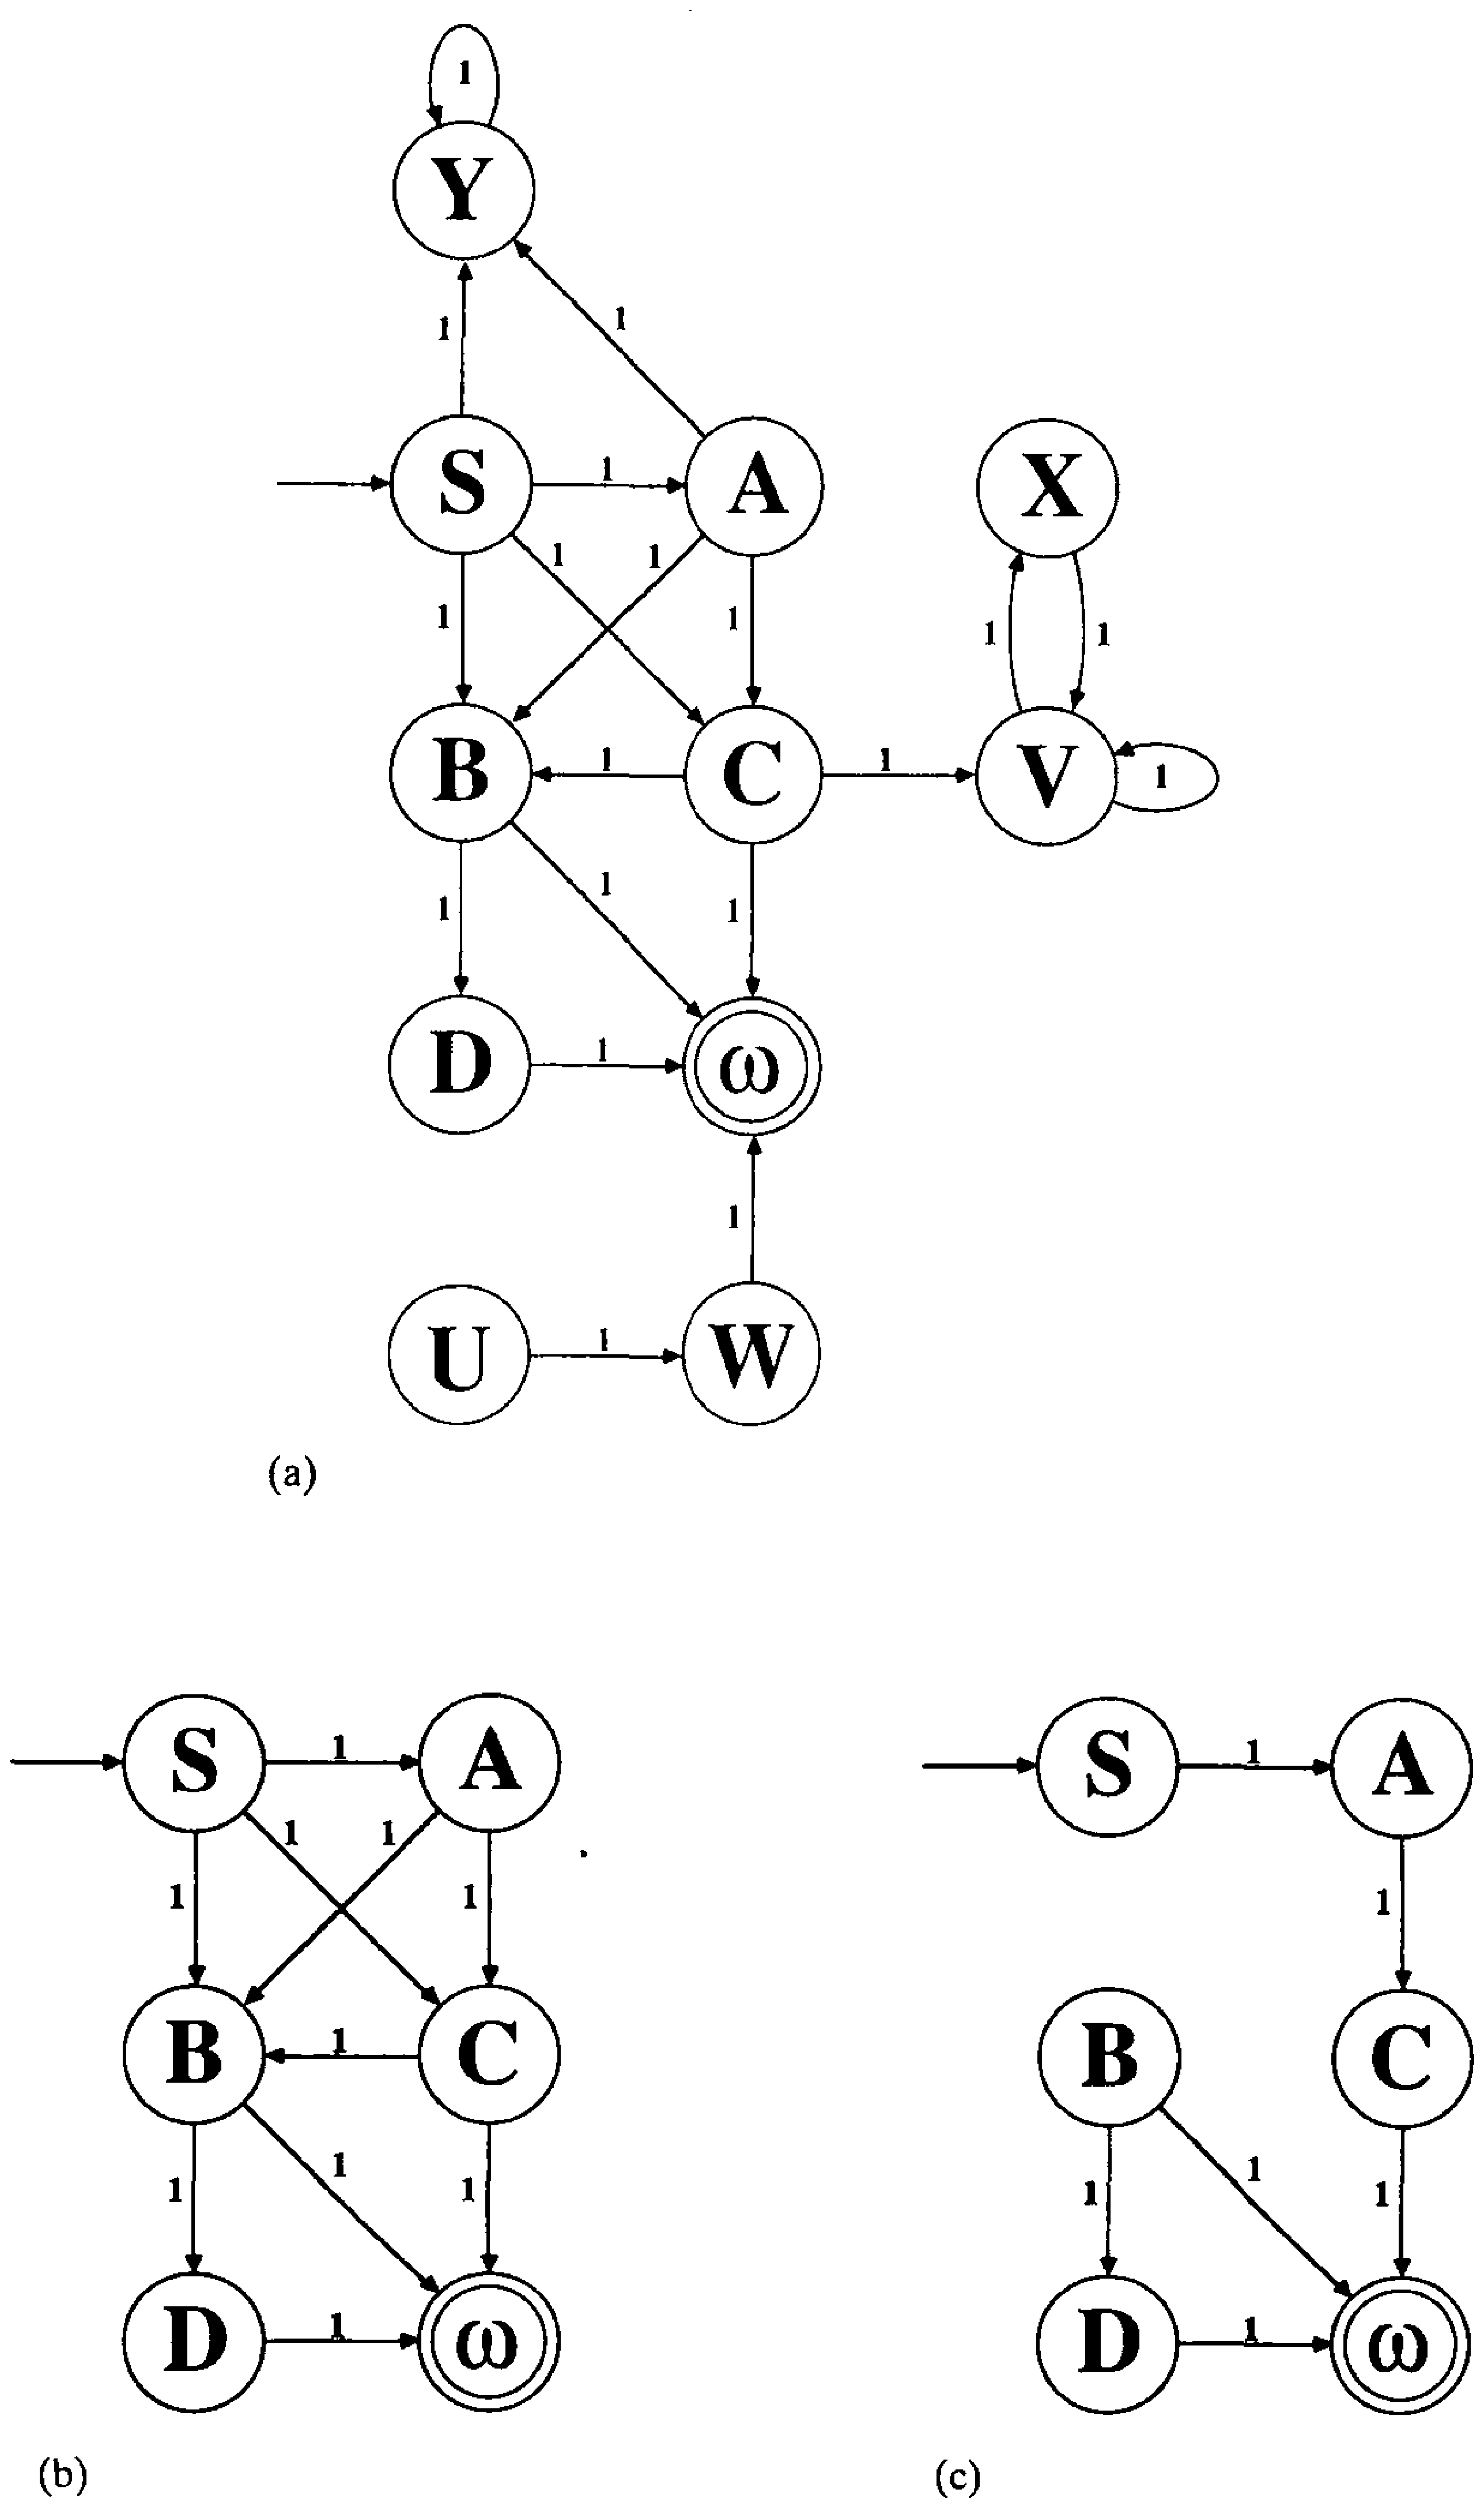
\epsfig{figure=ToFAfigures/fig9-11.eps,width=4.7in}}
\caption{(a) The automaton discussed in Example 9.12 (b) The simplified
automaton discussed in Example 9.12 (c) The final automaton discussed in
Example 9.12}\label{fig-9.11}
\end{figure}

Note that the algorithm developed in Theorem \ref{thm-9.3} relied on connectedness, and
hence the specification of the final states was unimportant in this approach.
With $\omega$ as the lone final state, some of the decision algorithms developed
in Chapter \ref{ch-12} could have been used in place of the connectivity and
accessibility checks.

Example 9.12 illustrates the simplification that can be attained by the
elimination of useless productions. Further convenience is afforded by the
elimination of nongenerative $A$-rules of the form $A\rightarrow B$. Recall that
in the grammar $\langle\{S_1,S_2,S_3,S_4,S_5\},\{\pmb{a},\pmb{b},\pmb{c}\},S_1,
\{S_1\rightarrow S_2,S_2\rightarrow S_3,S_3\rightarrow S_4,S_4\rightarrow S_5,
S_5\rightarrow\pmb{a}\}\rangle$, all the nonterminals were useful, but the
production set was still needlessly complex.

% Definition 9.8
\begin{dfn}\label{dfn-9.8}
A production of the form $A\rightarrow B$, where $A,B\in\Omega$, is called a
\emph{\Index{unit production}} or a \emph{\Index{nongenerative production}}.
\end{dfn}

As with the elimination of useless nonterminals, unit productions can be removed
with the help of automata constructs. The interested reader is referred to
[DENN] for the constructive proof. The proof given below indicates the general
algorithmic approach.

% Theorem 9.4
\begin{thm}\label{thm-9.4}
Every pure context-free language $L$ can be generated by a pure context-free
grammar which contains no useless non-terminals and no unit productions. Every
context-free language $L'$ can be generated by a context-free grammar which
contains no useless non-terminals and no unit productions except perhaps the
$Z$-rule $Z\rightarrow S$, where $Z$ is the new start symbol.

\emph{Proof.} If the first statement of the theorem is proved, the second will
follow immediately from Definition \ref{dfn-8.6}. If $L$ is a pure context-free language,
then by Definition \ref{dfn-8.5} there is a pure context-free grammar $G=\langle\Omega,
\Sigma,S,P\rangle$ that generates $L$. Divide the production set up into $P^u$
and $P^n$, the set of unit productions and the set of nonunit productions,
respectively. For each nonterminal $B$ found in $P^u$, find $B^u=\{C|B
\DRightarrow C\}$, the \emph{unit closure} of $B$. The derivations sought must
all come from the (finite) set $P^u$, and there is clearly an algorithm that
correctly calculates $B^u$. In fact, $B^u$ is represented by the set of
accessible states in a suitably defined automaton (see the exercises). Define a
new grammar $G'=\langle\Omega,\Sigma,S,P'\rangle$, where $P'=P^n\cup\{B
\rightarrow\alpha|B$ is a nonterminal in $P^u\wedge C\in B^u\wedge C\rightarrow
\alpha\in P^n\}$. A straightforward induction argument shows that $G'$ is
equivalent to $G$, and $G'$ contains no unit productions. Note that if $G$ is
pure, so is $G'$.

G' is likely to contain useless nonterminals, even if all the productions in $G$
were useful (see Example 9.13). However, the algorithm from Theorem \ref{thm-9.3} can now
be applied to $G'$ to eliminate useless nonterminals. Since that algorithm
creates no new productions, the resulting grammar will still be free of unit
productions.
\end{thm}

\subsection*{Example 9.13}

Consider again the pure context-free grammar
\[ \langle\{S_1,S_2,S_3,S_4,S_5\},\{\pmb{a},\pmb{b},\pmb{c}\},S_1,\{S_1
	\rightarrow S_2,S_2\rightarrow S_3,S_3\rightarrow S_4,S_4\rightarrow
	S_5,S_5\rightarrow\pmb{a}\}\rangle \]
The production set is split into $P^n = \{S_5\rightarrow\pmb{a}\}$ and
\[ P^u = \{S_1\rightarrow S_2,S_2\rightarrow S_3,S_3\rightarrow S_4,S_4
	\rightarrow S_5\}. \]
The unit-closure sets are
\begin{center}\begin{tabular}{r@{ = }l}
$S^u_1$ & $\{S_1,S_2,S_3,S_4,S_5\}$ \\
$S^u_2$ & $\{S_2,S_3,S_4,S_5\}$ \\
$S^u_3$ & $\{S_3,S_4,S_5\}$ \\
$S^u_4$ & $\{S_4,S_5\}$ \\
$S^u_5$ & $\{S_5\}$
\end{tabular}\end{center}
Since $S_5\rightarrow\pmb{a}$ and $S_5\in S^u_3$, the production $S_3\rightarrow
\pmb{a}$ is added to $P'$. The full set of productions is $P'=\{S_1\rightarrow
\pmb{a},S_2\rightarrow\pmb{a},S_3\rightarrow\pmb{a},S_4\rightarrow\pmb{a},S_5
\rightarrow\pmb{a}\}$. The elimination of useless nonterminals and productions
results in the grammar $\langle\{S_1\},\{\pmb{a},\pmb{b},\pmb{c}\},S_1,\{S_1
\rightarrow\pmb{a}\}\rangle$.

\subsection*{Example 9.14}

Consider the context-free grammar with productions
\begin{center}\begin{tabular}{r@{ $\rightarrow$ }l}
$Z$ & $S,\ Z\rightarrow\lambda$ \\
$S$ & $CB\pmb{h},\ S\rightarrow D$ \\
$A$ & $\pmb{aa}C$ \\
$B$ & $S\pmb{f},\ B\rightarrow\pmb{ggg}$ \\
$C$ & $\pmb{c}A,\ C\rightarrow\pmb{d},C\rightarrow C$ \\
$D$ & $E,\ D\rightarrow SABC$ \\
$E$ & $\pmb{be}$
\end{tabular}\end{center}
The unit closures of each of the appropriate nonterminals and the new
productions they imply are shown below. Note that $Z\rightarrow S$ is not
considered and that the productions suggested by $C\rightarrow C$ are already
present.
\begin{center}\begin{tabular}{r@{ \ $\DRightarrow$ }l@{$\qquad$}r@{ $\rightarrow$ }l}
$S$ & $D$ & $S$ & $SABC$ \\
$S$ & $E$ & $S$ & $\pmb{be}$ \\
$D$ & $E$ & $D$ & $\pmb{be}$ \\
$C$ & $C$ & $C$ & $\pmb{c}A,\ C\rightarrow\pmb{d}$
\end{tabular}\end{center}
The new set of productions is therefore
\begin{center}\begin{tabular}{r@{ $\rightarrow$ }l}
$Z$ & $S,\ Z\rightarrow\lambda$ \\
$S$ & $SABC,\ S\rightarrow\pmb{be},\ S\rightarrow CB\pmb{h}$ \\
$A$ & $\pmb{aa}C$ \\
$B$ & $S\pmb{f},\ B\rightarrow\pmb{ggg}$ \\
$C$ & $\pmb{c}A,\ C\rightarrow\pmb{d}$ \\
$D$ & $\pmb{be},\ D\rightarrow SABC$ \\
\end{tabular}\end{center}
Note that D is now useless and can be eliminated.

The assurance that every context-free grammar corresponds to an equivalent
grammar with no unit productions is helpful in many situations. In particular,
it is instrumental to the proof showing that the following restrictive type of
grammar is indeed a canonical form for context-free languages.

% Definition 9.9
\begin{dfn}\label{dfn-9.9}
A pure context-free grammar $G=\langle\Omega,\Sigma,S,P\rangle$ is in
\emph{pure Chomsky normal form}\index{pure Chomsky normal form|see{PCNF}} (\Index{PCNF}) if $P$ contains only
productions of the form $A\rightarrow BC$ and $A\rightarrow\pmb{d}$, where $B$
and $C$ are nonterminals and $\pmb{d}\in\Sigma$.

A context-free grammar $G=\langle\Omega,\Sigma,Z,P\rangle$ is in
\emph{Chomsky normal form}\index{Chomsky normal form|see{CNF}}(\Index{CNF}) if the $Z$-rules $Z\rightarrow
S$ and $Z\rightarrow\lambda$ are the only allowable productions involving the
start symbol $Z$, and all other productions are of the form $A\rightarrow BC$
and $A\rightarrow\pmb{d}$, where $B$ and $C$ are nonterminals and $\pmb{d}\in
\Sigma$.
\end{dfn}

Thus, in PCNF the grammatical rules are limited to producing exactly two
nonterminals or one terminal symbol. Few of the grammars discussed so far have
met the restricted criteria required by Chomsky normal form. However, every
context-free grammar can be transformed into an equivalent CNF grammar, as
indicated in the following proof. The basic strategy will be to add new
nonterminals and replace undesired productions such as $A\rightarrow JK\pmb{cb}$
by a set of equivalent productions in the proper form, such as $A\rightarrow
JY_{11},\ Y_{11}\rightarrow KY_{12},\ Y_{12}\rightarrow X_cX_b,\ X_c\rightarrow
\pmb{c},\ X_b\rightarrow\pmb{b}$, where $Y_{11},\ Y_{12},\ X_b$, and $X_c$ are
new nonterminals.

% Theorem 9.5
\begin{thm}\label{thm-9.5}
\ \\
\indent Every pure context-free language $L$ can be generated by a pure Chomsky normal
form grammar.

Every context-free language $L'$ can be generated by a Chomsky
normal form grammar.

\emph{Proof.} Again, if the first statement of the theorem is proved, the second
will follow immediately from Definition \ref{dfn-8.6}. If L is a pure context-free
language, then by Definition \ref{dfn-8.5} there is a pure context-free grammar $G=\langle
\Omega,\Sigma,S,P\rangle$ that generates $L$. Theorem \ref{thm-9.4} shows that without
loss of generality we may assume that P contains no unit productions. We
construct a new grammar $G'=\langle\Omega,\Sigma,S,P'\rangle$ in the following
manner. Number the productions in $P$, and consider each production in turn. If
the right side of the $k$th production consists of only a single symbol, then it
must be a terminal symbol, since there are no unit productions. No modifications
are necessary in this case, and the production is retained for use in the new
set of productions $P'$. The same is true if the kth production consists of two
symbols and they are both nonterminals. If one or both of the symbols is a
terminal, then the rule must be modified by replacing any terminal symbol {\bf
a} with a new nonterminal $X_{\pmb{a}}$. Whenever such a replacement is done, a
production of the form $X_{\pmb{a}}\rightarrow\pmb{a}$ must also be included in
the new set of productions $P'$. If the $k$th production is $A\rightarrow\alpha_1
\alpha_2\alpha_3\cdots\alpha_n$, where the number of (terminal and nonterminal)
symbols is $n>2$, then new nonterminals $Y_{k1},Y_{k2},\ldots,Y_{kn-2}$ must be
introduced and the rule must be replaced by the set of productions $A\rightarrow
\alpha_1Y_{k1},Y_{k1}\rightarrow\alpha_2Y_{k2},Y_{k2}\rightarrow\alpha_3Y_{k3},
\cdots Y_{kn-2}\rightarrow \alpha_{n-1}\alpha_n$. Again, if any $\alpha_i$ is a
terminal symbol such as $\pmb{a}$, it must be replaced as indicated earlier by the
nonterminal $X_{\pmb{a}}$.

Each new set of rules is clearly capable of producing the same effect as the
rule that was replaced. Each nonterminal $Y_{ki}$ is used in only one such
replacement set to ensure that the new rules do not combine in unexpected new
ways. Tedious but straightforward inductive proofs will justify that $L(G) =
L(G')$.
\end{thm}

\subsection*{Example 9.15}

The grammar discussed in Example 9.14 can be transformed into CNF by the
algorithm given in Theorem \ref{thm-9.5}. After elimination of the unit productions and
the consequent useless productions, the productions (suitably numbered) that
must be examined are

\begin{tabular}{l@{$\qquad\qquad\qquad$}l}
$\pmb{1.}\ \ S\rightarrow SABC$ & $\pmb{5.}\ \ B\rightarrow S\pmb{f}$ \\
$\pmb{2.}\ \ S\rightarrow\pmb{be}$ & $\pmb{6.}\ \ B\rightarrow\pmb{ggg}$ \\
$\pmb{3.}\ \ S\rightarrow CB\pmb{h}$ & $\pmb{7.}\ \ C\rightarrow\pmb{c}A$ \\
$\pmb{4.}\ \ A\rightarrow\pmb{aa}C$ & $\pmb{8.}\ \ C\rightarrow\pmb{d}$
\end{tabular}

\noindent In the corresponding lists given below, notice that only production 8
is retained; the others are replaced by
\begin{center}\begin{tabular}{r@{ $\rightarrow$ }l}
$S$ & $SY_{11},\ Y_{11}\rightarrow AY_{12},\ Y_{12}\rightarrow BC$ \\
$S$ & $X_{\pmb{b}}X_{\pmb{e}}$ \\
$S$ & $CY_{31},\ Y_{31}\rightarrow BX_{\pmb{h}}$ \\
$A$ & $X_{\pmb{a}}Y_{41},\ Y_{41}\rightarrow X_{\pmb{a}}C$ \\
$B$ & $SX_{\pmb{f}}$ \\
$B$ & $X_{\pmb{g}}Y_{61},\ Y_{61}\rightarrow X_{\pmb{g}}X_{\pmb{g}}$ \\
$C$ & $X_{\pmb{c}}A$ \\
$C$ & $\pmb{d}$
\end{tabular}\end{center}
and the terminal productions $X_{\pmb{b}}\rightarrow\pmb{b},\ X_{\pmb{e}}
\rightarrow\pmb{e},\ X_{\pmb{h}}\rightarrow\pmb{h},\ X_{\pmb{a}}\rightarrow
\pmb{a},\ X_{\pmb{f}}\rightarrow\pmb{f},\ X_{\pmb{g}}\rightarrow\pmb{g}$. Since
$\pmb{d}$ did not appear as part of a two-symbol production, the rule $X_{\pmb{d}}
\rightarrow\pmb{d}$ can be eliminated. The above rules, with $S$ as the start
symbol, form a pure Chomsky normal form grammar. The new start symbol $Z$ and
productions $Z\rightarrow S$ and $Z\rightarrow\lambda$ would be added to this
pure context-free grammar to obtain the required CNF.

Grammars in Chomsky normal form allow an exact correspondence to be made between
the length of a terminal string and the length of the derivation sequence that
produces that string. If the empty string can be derived, the production
sequence will consist of exactly one rule application ($Z\rightarrow\lambda$). A
simple inductive argument shows that, if a string of length $n>0$ can be derived,
the derivation sequence must contain exactly $2n$ steps. In the grammar derived
in Example 9.15, for example, the following terminal string of length 5 is
generated in exactly ten productions:
\begin{center}\begin{tabular}{r@{ $\Rightarrow$ }l}
$Z$ & $S\Rightarrow CY_{31} \Rightarrow \pmb{d}Y_{31} \Rightarrow \pmb{d}BX_h
	\Rightarrow \pmb{d}SX_fX_h \Rightarrow \pmb{d}X_bX_eX_fX_h \Rightarrow
	\pmb{db}X_eX_fX_h$ \\
& $\pmb{dbe}X_fX_h \Rightarrow \pmb{dbef}X_h \Rightarrow \pmb{dbefh}$
\end{tabular}\end{center}

Other useful properties are also assured for grammars in Chomsky normal form.
When a grammar is in CNF, all parse trees can be represented by binary trees,
and upper and lower bounds on the depth of a parse tree for a string of length
$n$ can be found (see the exercises). The derivational relationship between the
number of production steps used and the number of terminals produced implies
that CNF grammars generate an average of one terminal every two productions. The
following canonical form requires every production to contain at least one
terminal symbol, and grammars in this form must produce strings of length
$n(>0)$ in no more than $n$ steps.

% Definition 9.10
\begin{dfn}\label{dfn-9.10}
A pure context-free grammar $G=\langle\Omega,\Sigma,S,P\rangle$ is in
\emph{\Index{pure Greibach normal form}} (\Index{PGNF}) if $P$ contains only 
productions of the form $A\rightarrow\pmb{d}\alpha$, where $\alpha\in(\Omega\cup
\Sigma)^*$ and $d\in\Sigma$..

A context-free grammar $G=\langle\Omega,\Sigma,Z,P\rangle$ is in \emph{\Index{Greibach
normal form}} (\Index{GNF}) if the $Z$-rules $Z\rightarrow S$ and $Z\rightarrow
\lambda$ are the only allowable productions involving the start symbol $Z$, and
all other productions are of the form $A\rightarrow\pmb{d}\alpha$, where $\alpha
\in(\Omega\cup\Sigma)^*$ and $\pmb{d}\in\Sigma$.
\end{dfn}

In pure Greibach normal form, the grammatical rules are limited to producing at
least one terminal symbol as the first symbol. The original grammar in Example
9.9 is a PGNF grammar, but few of the other grammars presented in this chapter
meet the seemingly mild restrictions required for Greibach normal form. The main
obstacle to obtaining a GNF grammar is the possible presence of \emph{left
recursion}. A nonterminal A is called \emph{\Index{left recursive}} if there is
a sequence of one or more productions for which $A\ \DRightarrow A\beta$ for some
string $\beta$. Greibach normal form disallows such occurrences since no
production may produce a string starting with a nonterminal. Replacing
productions involved with left recursion is complex, but every context-free
grammar can be transformed into an equivalent GNF grammar, as shown by Theorem
\ref{thm-9.6}. Two techniques will be needed to transform the productions into the
appropriate form, and the following lemmas ensure that the grammatical
transformations leave the language unchanged. The first indicates how to remove
an $X$-rule that begins with an undesired nonterminal; Lemma \ref{lmm-9.1} specifies a new
set of productions that compensate for the loss.

% Lemma 9.1
\begin{lmm}\label{lmm-9.1}
Let $G=\langle\Omega,\Sigma,S,P\rangle$ be a context-free grammar, and assume
there is a string $\alpha$ and nonterminals $X$ and $B$ for which $X\rightarrow
B\alpha\in P$. Further assume that the set of all $B$-rules is given by $\{B
\rightarrow\beta_1,B\rightarrow\beta_2,\ldots,B\rightarrow\beta_m\}$ and let
$G'=\langle\Omega,\Sigma,S,P'\rangle$, where
\[ P'=P\cup\{X\rightarrow\beta_1\alpha,X\rightarrow\beta_2\alpha,\ldots,X
	\rightarrow\beta_m\alpha\} - \{X\rightarrow B\alpha\}. \]
Then $L(G) = L(G')$.

\emph{Proof.} Let each nonterminal $A$ be associated with the set of sentential
forms $X_A$ that $A$ can produce. That is, let $A=X_A=\{x\in(\Sigma\cup\Omega)^*|
A\ \DRightarrow x\}$. The nonterminals then denote variables in a set of language
equations that reflect the productions in $P$. These equations will generally
not be linear; several variables may be concatenated together within a single
term. Since the set of all $B$-rules were $B\rightarrow\beta_1,B\rightarrow
\beta_2,\ldots,B\rightarrow\beta_m,X_B$ satisfies the equation
\[ X_B = \beta_1 \cup \beta_2 \cup \cdots \cup \beta_m \]
Similarly, if the $X$-rules other than $X\rightarrow B\alpha$ are $X\rightarrow
\gamma_1,X\rightarrow \gamma_2,\ldots,X\rightarrow\gamma_n$, then $X$ satisfies
the equation
\[ X_X = \gamma_1\cup\gamma_2\cup\cdots\cup\gamma_n\cup X_B\alpha \]
Substituting for $X_B$ in the $X_X$ equation yields
\[ X_X = \gamma_1\cup\gamma_2\cup\cdots\cup\gamma_n\cup(\beta_1\cup\beta_2\cup
	\cdots\cup\beta_m)\alpha \]
which by the distributive law becomes
\[ X_X = \gamma_1\cup\gamma_2\cup\cdots\cup\gamma_n\cup\beta_1\alpha\cup\beta_2
	\alpha\cup\cdots\cup\beta_m\alpha \]
This shows why the productions $X\rightarrow\beta_1\alpha,X\rightarrow\beta_2
\alpha, \ldots ,X\rightarrow\beta_m\alpha$ can replace the rule $X\rightarrow B
\alpha$.
\end{lmm}
The type of replacement justified by Lemma \ref{lmm-9.1} will not eliminate left recursion.
The following lemma indicates a way to remove all the left-recursive $X$-rules
by introducing a new right-recursive nonterminal.

% Lemma 9.2
\begin{lmm}\label{lmm-9.2}
Let $G=\langle\Omega,\Sigma,S,P\rangle$ be a context-free grammar, and choose a
nonterminal $X\in\Omega$. Denote the set of all left-recursive $X$-rules by $X^r =
\{X\rightarrow X\alpha_1,X\rightarrow X\alpha_2,\ldots,X\rightarrow X\alpha_m\}$
and the set of all non[left]recursive X-rules by $X^n=\{X\rightarrow\gamma_1,X
\rightarrow\gamma_2,\ldots,X\rightarrow\gamma_n\}$. Choose a new nonterminal $Y
\notin\Omega$ and let $G'' = \langle\Omega\cup\{Y\},\Sigma,S,P''\rangle$, where
$P'' = P\cup\{X\rightarrow\gamma_1Y,X\rightarrow\gamma_2Y,\ldots,X\rightarrow
\gamma_nY\}\cup\{Y\rightarrow\alpha_1,Y\rightarrow\alpha_2,\ldots,Y\rightarrow
\alpha_m\}\cup\{Y\rightarrow\alpha_1Y,Y\rightarrow\alpha_2Y,\ldots,Y\rightarrow
\alpha_mY\}-X^r$. Then $L(G) = L(G'')$.

\emph{Proof.} As in Lemma \ref{lmm-9.1}, let each nonterminal $A$ be associated with the
set of sentential forms $X_A$ that $A$ can produce, and consider the set of
language equations generated by $P$. The $X_X$ equation is
\[ X_X = \gamma_1 \cup \gamma_2 \cup\cdots\cup \gamma_n \cup X_X\alpha_1 \cup
	X_X\alpha_2 \cup\cdots\cup X_X\alpha_m \]
Solving by the method indicated in Theorem \ref{thm-6.4}c for an equivalent expression
for $X_X$ shows that
\[ X_X = (\gamma_1\cup\gamma_2\cup\cdots\cup\gamma_n)(\alpha_1\cup\alpha_2\cup
	\cdots\cup\alpha_m)^* \]
In the new set of productions $P''$, the equations of interest are
\begin{center}\begin{tabular}{l}
$X_X = \gamma_1\cup\gamma_2\cup\cdots\cup\gamma_n\cup\gamma_1X_Y\cup\gamma_2X_Y
	\cup\cdots\cup\gamma_nX_Y$ \\
$X_Y = \alpha_1\cup\alpha_2\cup\cdots\cup\alpha_m\cup\alpha_1X_Y\cup\alpha_2X_Y
	\cup\cdots\cup\alpha_mX_Y$
\end{tabular}\end{center}
Factoring each equation produces
\begin{center}\begin{tabular}{l}
$X_X = \gamma_1\cup\gamma_2\cup\cdots\cup\gamma_n\cup(\gamma_1\cup\gamma_2\cup
	\cdots\cup\gamma_n)X_Y$ \\
$X_Y = \alpha_1\cup\alpha_2\cup\cdots\cup\alpha_m\cup(\alpha_1\cup\alpha_2\cup
	\cdots\cup\alpha_m)X_Y$
\end{tabular}\end{center}
and the second can also be solved for an equivalent expression for $X_Y$,
yielding
\[ X_Y = (\alpha_1\cup\alpha_2\cup\cdots\cup\alpha_m)^*(\alpha_1\cup\alpha_2\cup
	\cdots\cup\alpha_m) \]
Substituting this expression for $X_Y$ in the $X_X$ equation produces
\[ X_X = \gamma_1\cup\gamma_2\cup\cdots\cup\gamma_n\cup(\gamma_1\cup\gamma_2\cup\cdots
	\cup\gamma_n)(\alpha_1\cup\alpha_2\cup\cdots\cup\alpha_m)^*(\alpha_1\cup
	\alpha_2\cup\cdots\cup\alpha_m) \]
which by the distributive law becomes
\[ X_X = (\gamma_1\cup\gamma_2\cup\cdots\cup\gamma_n)(\lambda\cup(\alpha_1\cup
	\alpha_2\cup\cdots\cup\alpha_m)^*(\alpha_1\cup\alpha_2\cup\cdots\cup
	\alpha_m)) \]
Using the fact that $\lambda\cup B^*B = B^*$, this simplifies to
\[ X_X = (\gamma_1\cup\gamma_2\cup\cdots\cup\gamma_n)(\alpha_1\cup\alpha_2\cup
	\cdots\cup\alpha_m)^* \]
Therefore, when $X_Y$ is eliminated from the sentential forms, $X_X$ produces
exactly the same strings as before. This indicates why the productions in the
sets
\begin{center}\begin{tabular}{l}
$\{X\rightarrow \gamma_1Y,X\rightarrow\gamma_2Y,\ldots,X\rightarrow\gamma_nY\}
	\cup\{\rightarrow\alpha_1,Y\rightarrow\alpha_2,\ldots,Y\rightarrow
	\alpha_m\}\cup$ \\
$\{Y\rightarrow\alpha_1Y,Y\rightarrow\alpha_2Y,\ldots,Y\rightarrow\alpha_mY\}$
\end{tabular}\end{center}
can replace the left-recursive $X$-rules $X\rightarrow\gamma_1,\ X\rightarrow\gamma_2,
\ldots,X\rightarrow\gamma_n$.
\end{lmm}

Note that the new production set eliminates all left-recursive $X$-rules and does not
introduce any new left-recursive productions. The techniques discussed in Lemmas \ref{lmm-9.1}
and \ref{lmm-9.2}, when applied in the proper order, will transform any context-free
grammar into one that is in Greibach normal form. The appropriate sequence is
given in the next theorem.

% Theorem 9.6
\begin{thm}\label{thm-9.6}
\ \\
\indent Every pure context-free language $L$ can be generated by a pure Greibach normal
form grammar.

Every context-free language $L'$ can be generated by a Greibach normal form
grammar.

\emph{Proof.} Because of Definition \ref{dfn-8.6}, the second statement will follow
immediately from the first. If $L$ is a pure context-free language, then
there is a pure context-free grammar
$G=\langle\{S_1,S_2,\ldots,S_r\},\Sigma,S_1,P\rangle$ that generates $L$ 
(by Definition \ref{dfn-8.5}). We construct a new grammar by
applying the transformations discussed in the previous lemmas.

\emph{Phase 1:} The replacements suggested by Lemmas \ref{lmm-9.1} and \ref{lmm-9.2} will be used to
ensure that the \emph{increasing condition} is met: if $S_i\rightarrow S_j\alpha$
belongs to the new grammar, then $i>j$. We transform the $S_k$ rules for $k = r,
r-1,\ldots,2,1$ (in that order), considering the productions for each
nonterminal in turn. At the end of the $i$th iteration, the top $i$ nonterminals
will conform to the increasing condition. After the final step, all nonterminals
(including any newly introduced ones) will conform, all left recursion will be
eliminated, and we can proceed to phase 2.

The procedure for the $i$th iteration is: If an $S_i$-rule of the form $S_i
\rightarrow S_j\alpha$ is found where $i<j$. eliminate it as specified in Lemma
\ref{lmm-9.1}. This may introduce other rules of the form $S_i\rightarrow S_{j'}\alpha'$, in
which $i$ is still less than $j'$. Such new rules will likewise have to be
eliminated via Lemma \ref{lmm-9.1}, but since the offending subscript will decrease each
time, this process will eventually terminate. $S_i$-rules of the form $S_i
\rightarrow S_j\alpha$ where $i=j$ can then be eliminated according to Lemma \ref{lmm-9.2}.
This will introduce some new nonterminals, which can be given new,
higher-numbered subscripts. Lemma \ref{lmm-9.2} is designed so that the new rules will
automatically satisfy the increasing condition specified earlier. The remaining
$S_i$-rules must then conform to the increasing condition. The process continues
with lower-numbered rules until all the rules in the new production set conform
to the increasing condition.

\emph{Phase 2:} At this point, $S_1$ conforms to the increasing condition, and
since there are no nonterminals with subscripts that are less than 1, all the
$S_1$-rules must begin with terminal symbols, as required by GNF. The only $S_2$
rules that may not conform to GNF are those of the form $S_2\rightarrow S_1
\alpha$, and Lemma \ref{lmm-9.1} can eliminate such rules by replacing them with the
$S_1$-rules. Since all the $S_1$-rules now begin with terminal symbols, all the
new $S_2$-rules will have the same property. This process is applied to
$S_k$-rules for increasing k until the entire production set conforms to GNF.

The resulting context-free grammar is in GNF, and since all modifications were
of the type allowed by Lemmas \ref{lmm-9.1} and \ref{lmm-9.2}, the new grammar is equivalent to the
original.
\end{thm}

\subsection*{Example 9.16}

Consider the pure context-free grammar
\[ \langle\{S_1,S_2,S_3\},\{\pmb{a},\pmb{b},\pmb{c},\pmb{d},\pmb{e}\},S_1,
	\{S_1\rightarrow S_1S_2\pmb{c},S_1\rightarrow S_3\pmb{b}S_3,S_2
	\rightarrow S_1S_1,S_2\rightarrow\pmb{d},S_3\rightarrow S_2\pmb{e}\}
	\rangle \]
If the given subscript ordering is not the most convenient, the nonterminals
can be renumbered. The current ordering will minimize the number of
transformations needed to produce Greibach normal form, since the only
production that does not conform to the increasing condition is $S_1\rightarrow
S_3\pmb{b}S_3$. Thus, the first and second steps of phase 1 are trivially
completed; no substitutions are necessary. In the third step, Lemma \ref{lmm-9.1} allows
the offending production
\[ S_1 \rightarrow S_3\pmb{b}S_3 \]
to be replaced by
\[ S_1 \rightarrow S_2\pmb{eb}S_3 \]
The new production produces the smaller-subscripted nonterminal $S_2$, but the
new rule still does not satisfy the increasing condition. Replacing $S_1
\rightarrow S_2\pmb{eb}S_3$ as indicated by Lemma \ref{lmm-9.1} yields the two productions
\[ S_1 \rightarrow S_1S_1\pmb{eb}S_3\qquad\text{ and }\qquad S_1 \rightarrow
	\pmb{deb}S_3 \]
At this point, the grammar contains the productions
\[ S_1 \rightarrow S_1S_2\pmb{c},\quad S_1\rightarrow S_1S_1\pmb{eb}S_3,\quad
	S_1\rightarrow\pmb{deb}S_3,\quad S_2\rightarrow S_1S_1,\quad S_2
	\rightarrow\pmb{d},\quad S_3\rightarrow S_2\pmb{e} \]
The first nonterminal has a left-recursive rule that must be eliminated by
introducing the new nonterminal $S_4$. In the notation of Lemma \ref{lmm-9.2}, $n=1$,
$m=2$, $\gamma_1=\pmb{deb}S_3$, $\alpha_1 = S_2\pmb{c}$, and $\alpha_2 = S_1
\pmb{eb}S_3$. Eliminating $S_1\rightarrow S_1S_2\pmb{c}$ and $S_1\rightarrow
S_1S_1\pmb{eb}S_3$ introduces the new nonterminal $Y = S_4$ and the productions
\[ S_1\rightarrow\pmb{deb}S_3S_4,\quad S_4\rightarrow S_2\pmb{c},\quad S_4
	\rightarrow S_1\pmb{eb}S_3,\quad S_4\rightarrow S_2\pmb{c}S_4,\quad S_4
	\rightarrow S_1\pmb{eb}S_3S_4 \]
Phase 1 is now complete. All left-recursion has been eliminated and the grammar
now contains the productions
\begin{center}\begin{tabular}{l}
$S_1 \rightarrow \pmb{deb}S_3S_4,\quad S_1 \rightarrow \pmb{deb}S_3$ \\
$S_2 \rightarrow S_1S_1,\quad S_2 \rightarrow \pmb{d}$ \\
$S_3 \rightarrow S_2\pmb{e}$ \\
$S_4 \rightarrow S_2\pmb{c},\quad S_4 \rightarrow S_1\pmb{eb}S_3,\quad S_4 
	\rightarrow S_2\pmb{c}S_4,\quad S_4 \rightarrow S_1\pmb{eb}S_3S_4$
\end{tabular}\end{center}
all of which satisfy the increasing condition. The grammar is now set up for
phase 2, in which substitutions specified by Lemma \ref{lmm-9.1} will ensure that every
rule begins with a nonterminal.

The $S_1$-rules are in acceptable form, as is the $S_2$-rule $S_2\rightarrow
\pmb{d}$. The other $S_2$-rule, $S_2\rightarrow S_1S_1$, is replaced via Lemma
\ref{lmm-9.1} with $S_2 \rightarrow \pmb{deb}S_3S_4S_1$ and $S_2\rightarrow\pmb{deb}S_3S_1$.
Replacement of the $S_3$-rule then yields $S_3\rightarrow\pmb{deb}S_3S_4S_1
\pmb{e}$, $S_3\rightarrow\pmb{deb}S_3S_1\pmb{e}$ and $S_3\rightarrow\pmb{de}$.

The $S_4$ rules are treated similarly. The final set of productions at the
completion of phase 2 contains
\begin{center}\begin{tabular}{l}
$S_1\rightarrow\pmb{deb}S_3S_4,\quad S_1\rightarrow\pmb{deb}S_3$ \\
$S_2\rightarrow\pmb{deb}S_3S_4S_1,\quad S_2 \rightarrow \pmb{deb}S_3S_1,\quad
	S_2\rightarrow\pmb{d}$ \\
$S_3\rightarrow\pmb{deb}S_3S_4S_1\pmb{e},\quad S_3\rightarrow\pmb{deb}S_3S_1
	\pmb{e},\quad S_3\rightarrow\pmb{de}$ \\
$S_4\rightarrow\pmb{dc},\quad S_4\rightarrow\pmb{deb}S_3S_4S_1\pmb{c},\quad
	S_4\rightarrow\pmb{deb}S_3S_1\pmb{c},\quad S_4\rightarrow\pmb{deb}S_3
	S_4\pmb{eb}S_3,\quad S_4\rightarrow\pmb{deb}S_3\pmb{eb}S_3,$ \\
$S_4\rightarrow\pmb{deb}S_3S_4S_1\pmb{c}S_4,$ \\
$S_4\rightarrow\pmb{dc}S_4,\quad S_4\rightarrow\pmb{deb}S_3S_1\pmb{c}S_4,\quad
	S_4\rightarrow\pmb{deb}S_3S_4\pmb{eb}S_3S_4,\quad S_4\rightarrow
	\pmb{deb}S_3\pmb{eb}S_3S_4$
\end{tabular}\end{center}
In this grammar, $S_2$ is now useless and can be eliminated.

Greibach normal form is sometimes considered to require all productions to be of
the form $A\rightarrow\pmb{d}\alpha$, where $\alpha\in\Omega^*$ and $\pmb{d}\in
\Sigma$. Such rules must produce exactly one leading terminal symbol; the rest
of the string must be exclusively nonterminals. It should be clear that this
extra restriction can always be enforced by a technique similar to the one
employed for Chomsky normal form. The above conversion process would be extended
to \emph{phase 3}, in which unwanted terminals such as $\pmb{e}$ are replaced by a
new nonterminal $X_{\pmb{e}}$, and new productions such as $X_{\pmb{e}}
\rightarrow \pmb{e}$ are introduced. For the grammar in Example 9.16, the first
production might look like $S_1\rightarrow\pmb{d}X_{\pmb{e}}X_{\pmb{b}}S_3S_4$.

\section{Pumping Theorem}\label{9.4}

As was the case with type 3 languages, some languages are too complex to be
defined by a context-free grammar. To prove a language L is context-free, one
need only define a [context-free] grammar that generates L. By contrast, to prove L is not
context free, one must effectively argue that \emph{no} context-free grammar can
possibly generate $L$. The pumping lemma for deterministic finite automata
(Theorem \ref{thm-2.3}) showed that the repetition of patterns within strings accepted by
a DFA was a consequence of the nature of the finite description. The finiteness
of grammatical descriptions likewise implies a pumping theorem for languages
represented by context-free grammars. The proof is greatly simplified by the
properties implied by the existence of canonical forms for context-free
grammars.

% Theorem 9.7
\begin{thm}\label{thm-9.7}
Let $L$ be a context-free language over $\Sigma^*$. Then \\
$(\exists n\in\NN)(\forall z\in L \ni |z| \geq n)(\exists u,v,w,x,y \in
\Sigma^*)\ni z = uvwxy,\ |vwx| \leq n,\ |vx|\geq 1$, and $(\forall i\in\NN)(uv^i
wx^iy \in L)$

\emph{Proof.} Given a context-free language $L$, there must exist a PCNF grammar
$G=\langle\Omega,\Sigma,S,P\rangle$ generating $L-\{\lambda\}$. Let $k =
\|\Omega\|$. The parse tree generated by this PCNF grammar for any word $z\in L$
is a binary tree with each (terminal) symbol in $z$ corresponding to a distinct
leaf in the tree. Let $n=2^{k+1}$. Choose a string $z$ generated by $G$ of
length at least $n$ (if there are no strings in $L$ that are this long, then
the theorem is vacuously true, and we are done). The binary parse tree for any
such string $z$ must have depth at least $k+1$, which implies the existence of a
path involving at least $k+2$ nodes, beginning at the root and terminating with
a leaf. The labels on the $k+1$ interior nodes along the path must all be
nonterminals, and since $\|\Omega\| = k$, they cannot all be distinct. Indeed,
the repetition must occur within the ``bottom'' $k+1$ interior nodes along the
path. Call the repeated label R (see Figure \ref{fig-9.12}), and note that there must
exist a derivation for the parse tree that looks like
\[ S\ \DRightarrow u\R y\ \DRightarrow uv\R xy\ \DRightarrow uvwxy \]
where $u,\ v,\ w,\ x$, and $y$ are all terminal strings and $z=uvwxy$. That is,
there are productions in $P$ that allow $\R\ \DRightarrow v\R x$ and $\R
\ \DRightarrow w$. Since $S\ \DRightarrow u\R y$ and $R\ \DRightarrow w$, $S\ 
\DRightarrow uwy$ is a valid derivation, and $uwy$ is therefore a word in $L$.
Similarly, $S\ \DRightarrow u\R y\ \DRightarrow uv\R xy\ \DRightarrow uvv\R xxy
\ \DRightarrow uvvwxxy$, and so $uv^2wx^2y\in L$. Induction shows that each of the
strings $uv^i\!wx^i\!y$ belongs to $L$ for $i=0,1,2,\ldots$. If both $v$ and $x$
were empty, these strings would not be distinct words in $L$. This case cannot
arise, as shown next, and thus the existence of the ``long'' string $z \in L$ implies that there is an
infinite sequence of strings that must belong to $L$.

% Figure 9.12
\begin{figure}
\centerline{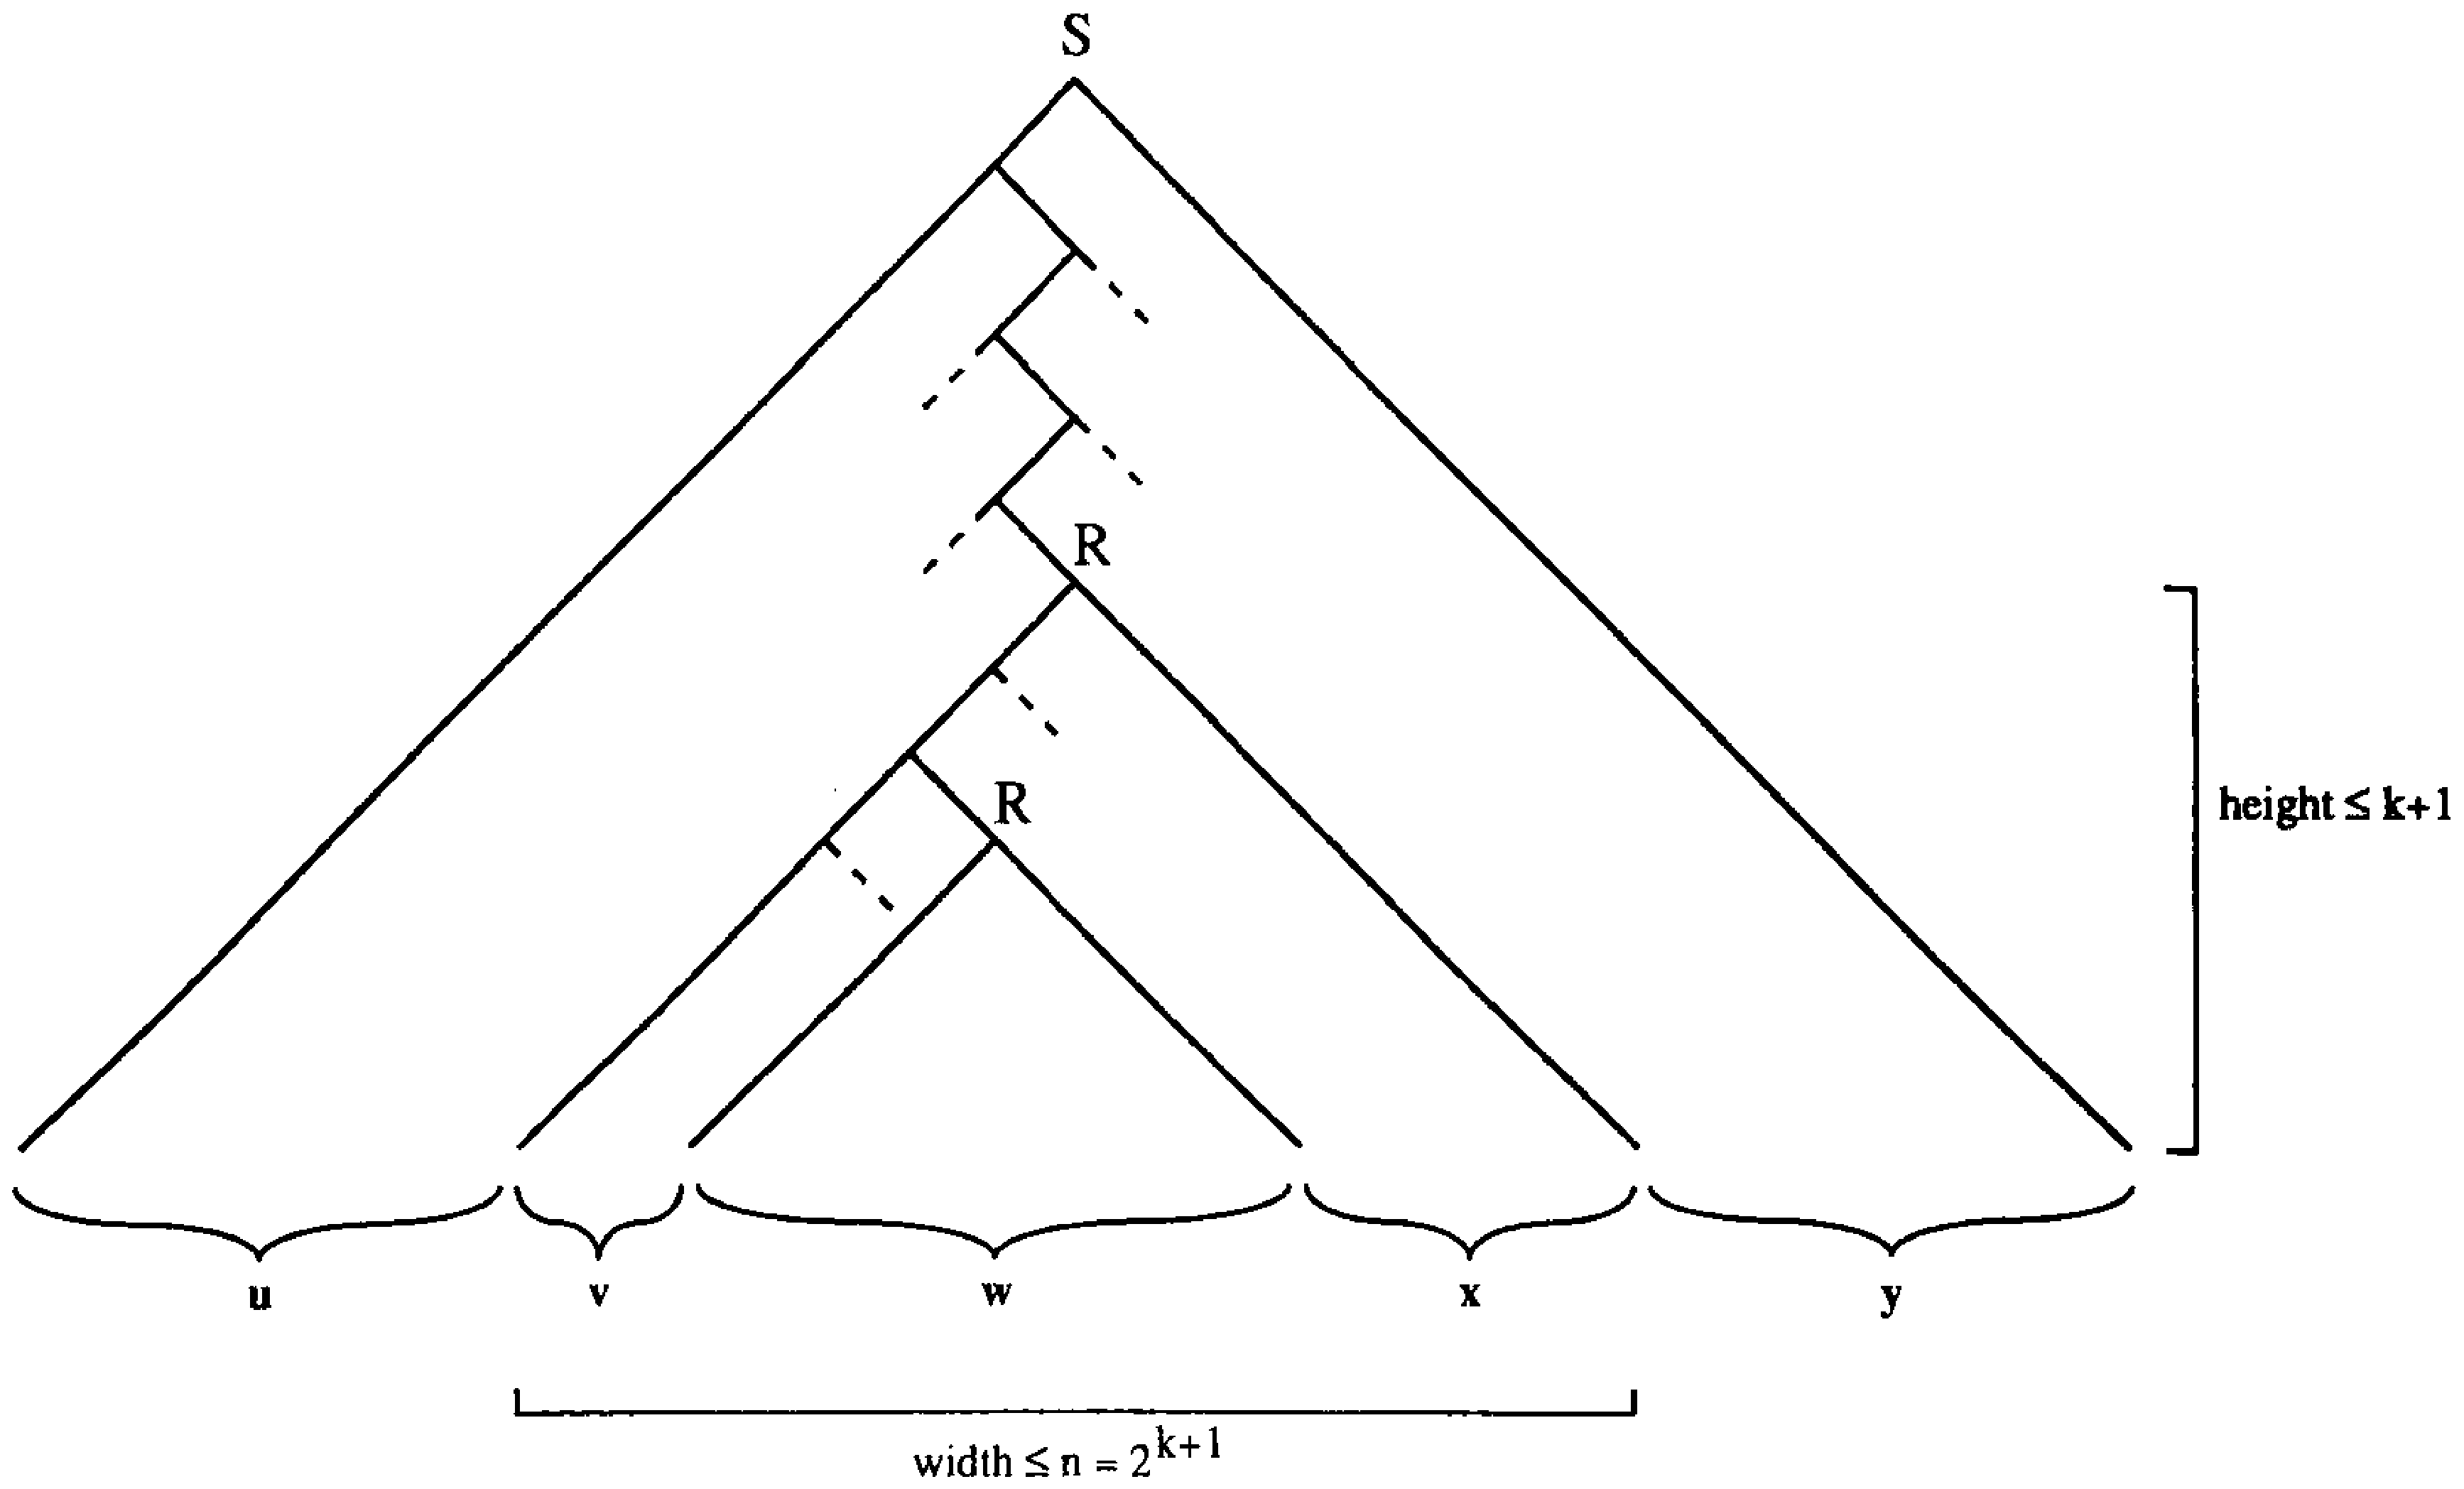
\epsfig{figure=ToFAfigures/fig9-12.eps,height=3.7in}}
\caption{The parse tree discussed in the proof of Theorem \ref{thm-9.7}}\label{fig-9.12}
\end{figure}

The two occurrences of R were in distinct places in the parse tree, and hence at
least one production was applied in deriving $uv\R xy$ from $u\R y$. Since the
PCNF grammar $G$ contains neither contracting productions nor unit productions,
the sentential form $uv\R xy$ must be of greater length than $u\R y$, and hence
$|v|+|x|>0$. Furthermore, the subtree rooted at the higher occurrence of R was
of height $k+1$ or less, and hence accounts for no more than $2^{k+1}(=n)$
terminals. Thus, $|vwx| \leq n$.\index{height of a parse tree}
All the criteria described in the pumping theorem are therefore met.

Since a
context-free language must be generated by a CNF grammar with a finite number of
nonterminals, there must exist a constant $n$ (such as $n = 2^{(\|\Omega\|+1)}$)
for which the existence of a string of length at least $n$ implies the existence
of an infinite sequence of distinct strings that must all belong to $L$, as
stated in the theorem.
\end{thm}

As with the pumping lemma, the pumping theorem is usually applied to justify
that certain languages are complex (by proving that the language does not
satisfy the pumping theorem and is thus not context free). Such proofs naturally
employ the contrapositive of Theorem \ref{thm-9.7}, which is stated next.

% Theorem 9.8
\begin{thm}\label{thm-9.8}
Let $L$ be a language over $\Sigma^*$. \\
{\bf if} $(\forall n\in\NN)(\exists z\in L \ni |z| \geq n)(\forall u,v,w,x,y \in
\Sigma^* \ni z = uvwxy, |vwx| \leq n, |vx|\geq 1)(\exists i\in\NN \ni uv^iwx^iy
\notin L)$ \\
{\bf then} $L$ is not context free.

\emph{Proof.} See the exercises.
\end{thm}

Examples 8.5 and 9.17 show that there are context-sensitive languages which are
not context free.

\subsection*{Example 9.17}

The language $L=\{a^kb^kc^k|\ k\in\NN\}$ is not a context-free language. Let $n$
be given, and choose $z=a^nb^nc^n$. Then $z\in L$ and $|z|= 3n \geq n$. If $L$
were context free, there must be choices for $u,\ v,\ w,\ x$, and $y$ satisfying
the pumping theorem. Every possible choice of these strings leads to a
contradiction, and hence $L$ cannot be context free. A sampling of the various
cases is outlined below.

If the strings $v$ and $x$ contain only one type of letter (for example, {\bf
c}), then $uv^2wx^2y$ will contain more $\pmb{c}$s than $\pmb{a}$s or $\pmb{b}$s, and
thus $uv^2wx^2y \notin L$. If $v$ were, say, all $\pmb{b}$s and $x$ were all {\bf
c}s, then $uv^2wx^2y$ would contain too few $\pmb{a}$s and would again not be a
member of $L$. If $v$ were to contain two types of letters such as $v =
\pmb{aabb}$, then $uv^2wx^2y = uvvwxxy = u\pmb{aabbaabb}wxxy$ and would
represent a string that had some $\pmb{b}$s preceding some $\pmb{a}$s, and again
$uv^2wx^2y \notin L$. All other cases are similar to these, and they
collectively imply that $L$ is not a context-free language.
[The shortest choice for $vwx$ that can successfully be pumped is
$\pmb{ab}^n\pmb{c}$, but this violates the condition that $|vwx| \leq n$.]

Example 9.17 illustrates one major inconvenience of the pumping theorem: the
inability to specify which portion of the string is to be ``pumped.'' With the
pumping lemma in Chapter \ref{ch-2}, variants were explored that allowed the first $n$
letters to be pumped or the last $n$ letters to be pumped. Indeed, any $n$
consecutive letters in a word from an FAD language can be pumped. For
context-free languages, such precision is more elusive. The uncertainty as to
where the $vwx$ portion of the string was in Example 9.17 led to many subcases,
since all combinations of $u,\ v,\ w,\ x$, and $y$ had to be shown to lead to
contradictions. The following result, a variant of Ogden's lemma, allows some
choice in the placement of the portion of the string to be pumped in a ``long''
word from a context-free language.

% Theorem 9.9
\begin{thm}\label{thm-9.9}
Let $L$ be a context-free language over $\Sigma^*$. Then \\
$(\exists n\in\NN)$ \\
$(\forall z \in L \ni |z| \geq n$ and $z$ has any $n$ or more positions marked
as distinguished) \\
$(\exists u,v,w,x,y \in\Sigma^*) \ni z = uvwxy$, \\
$vwx$ contains no more than $n$ distinguished positions, \\
$vx$ contains at least one distinguished position, \\
$w$ contains at least one distinguished position, and \\
$(\forall i \in\NN)(uv^iwx^iy \in L)$

\emph{Proof.} Given a context-free language $L$, there must exist a PCNF grammar
$G=\langle\Omega,\Sigma,S,P\rangle$ generating $L - \{\lambda\}$. Let $n =
2^{\|\Omega\|+1}$. The proof is similar to that given for the pumping theorem
(Theorem \ref{thm-9.7}); the method for choosing the path now depends on the placement of
the distinguished positions. A suitable path is constructed by beginning at the
root of the binary parse tree and, at each level, descending to the right or
left to lengthen the path. The decision to go right or left is determined by
observing the number of distinguished positions generated in the right subtree
and the number of distinguished positions generated in the left subtree. The
path should descend into the subtree that has the larger number of distinguished
positions; ties can be broken arbitrarily. The resulting path will terminate at
a leaf corresponding to a distinguished position, will be of sufficient length
to guarantee a repeated label R within the bottom $\|\Omega\| + 1$ interior
nodes, and so on. The conclusions now follow in much the same manner as those
given in the pumping theorem.
\end{thm}

\subsection*{Example 9.18}

For the language $L=\{\pmb{a}^k\pmb{b}^k\pmb{c}^k|k \in\NN\}$ investigated in
Example 9.17, Ogden's lemma could be applied with the first $n$ letters of
$\pmb{a}^n\pmb{b}^n\pmb{c}^n$ as the distinguished positions. Since $w$ must
have at least one distinguished letter (that is, an $\pmb{a}$), and $u$ and $v$
must precede $w$, the $u$ and $v$ portions of the string would then be required
to be all $\pmb{a}$s. This greatly reduces the number of cases that must be
considered. Note that more than $n$ letters can be chosen as the distinguished
positions, and they need not be consecutive.

\section{Closure Properties}\label{9.5}

Recall that \CSIG\ represented the class of context-free languages over $\Sigma$.
The applications of the pumping theorem show that not every language is context
free. The ability to show that specific languages are not context free makes it
feasible to decide which language operators preserve context-free languages. The
context-free languages are closed under most of the operators considered in
Chapter \ref{ch-5}; the major exceptions are complement and intersection. We begin with a
definition of substitution for context-free languages.

% Definition 9.11
\begin{dfn}\label{dfn-9.11}
Let $\Sigma=\{\pmb{a}_1,\pmb{a}_2,\ldots,\pmb{a}_m\}$ be an alphabet and let
$\Gamma$ be a second alphabet. Given context-free languages $L_1,L_2,\ldots,L_m$
over $\Gamma$, define a \emph{\Index{substitution}} $s$: $\Sigma\rightarrow\wp
(\Gamma^*)$ by $s(\pmb{a}_i) = L_i$ for each $i=1,2,\ldots,m$, which can be
extended to $\overline{s}$: $\Sigma^* \rightarrow \wp(\Gamma^*)$ by
\[ \overline{s}(\lambda) = \lambda \]
and
\[ (\forall\pmb{a}\in\Sigma)(\forall x\in\Sigma^*)(\overline{s}(\pmb{a}\cdot x)
	= s(\pmb{a})\cdot\overline{s}(x)) \]
$\overline{s}$ can be further extended to operate on a language $L\subseteq
\Sigma^*$ by defining $\overline{s}$: $\wp(\Sigma^*)\rightarrow\wp(\Gamma^*)$,
where
\[ \overline{s}(L) = \bigcup\limits_{z\in L} \overline{s}(z) \]
\end{dfn}

A substitution is similar to a language homomorphism (Definition \ref{dfn-5.8}), where
letters were replaced by single words, and to the regular set substitution given
by Definition \ref{dfn-6.5}. For context-free languages, substitution denotes the
consistent replacement of the individual letters within each word of a
context-free language with sets of words. Each such set of words must also be a
context-free language, although not necessarily over the original alphabet.

\subsection*{Example 9.19}

Let $L=L(G_t)$, where
\[ G_t = \langle\{T\},\{\pmb{a},\pmb{b},\pmb{c},\pmb{d},\pmb{-}\},T,\{T
	\rightarrow\pmb{a}|\pmb{b}|\pmb{c}|\pmb{d}|T\pmb{-}T\}\rangle \]
\begin{center}\begin{tabular}{l}
Let $L_1$ denote the set of all valid FORTRAN identifiers. \\
Let $L_2$ denote the set of all strings denoting integer constants. \\
Let $L_3$ denote the set of all strings denoting real constants. \\
Let $L_4$ denote the set of all strings denoting double-precision constants. \\
\end{tabular}\end{center}
If the substitution $s$ were defined by $s(\pmb{a})=L_1,\ s(\pmb{b})=L_2,\ s(
\pmb{c})=L_3,\ s(\pmb{d})=L_4$, then $\overline{s}(L)$ would represent the set
of all unparenthesized FORTRAN expressions involving only the subtraction
operator.

In this example, $\overline{s}(L)$ is a language over a significant portion of
the ASCII alphabet, whereas the original alphabet consisted of only five symbols.
The result is still context free, and this can be proved for all substitutions
of context-free languages into context-free languages. In Example 9.19, the
languages $L_1$, through $L_4$ were not only context free, but were in fact
regular. There are clearly context-free grammars defining each of them, and it
should be obvious how to modify $G_t$ to produce a grammar that generates
$\overline{s}(L)$. If $G_1=\langle\Omega_1,\Sigma_1,S_1,P_1\rangle$ is a grammar
generating $L_1$ [perhaps using the productions shown in Example 8.1], for example, then occurrences of a in the productions of $G_t$
should simply be replaced by the start symbol $S_1$ of $G_1$ and the productions
of $P_1$ added to the new grammar that will generate $\overline{s}(L)$. This is
essentially the technique used to justify Theorem \ref{thm-9.10}. The closure theorem is
stated for substitutions that do not modify the terminal alphabet, but it is
also true in general, as a trivial modification of the following proof would
show.

% Theorem 9.10
\begin{thm}\label{thm-9.10}\index{closure!under substitution}\index{substitution!context free}
Let $\Sigma$ be an alphabet, and let $s$: $\Sigma\rightarrow\Sigma^*$ be a
substitution. Then \CSIG\ is closed under $\overline{s}$.

\emph{Proof.} Let $\Sigma=\{\pmb{a}_1,\pmb{a}_2,\ldots,\pmb{a}_m\}$. If $L$ is a
context-free language, then there is a context-free grammar $G=\langle\Omega,
\Sigma,S,P\rangle$ that generates $L_1$. If $s$: $\Sigma\rightarrow\Sigma^*$ is
a substitution satisfying Definition \ref{dfn-9.11}, then for each letter $\pmb{a}_k\in
\Sigma$ there is a corresponding grammar $G_k=\langle\Omega_k,\Sigma_k,S_k,P_k
\rangle$ for which $L(G_k)=s(\pmb{a}_k)$. Since nonterminals can be freely
renamed, we may assume that $\Omega,\Omega_1,\Omega_2,\ldots,\Omega_m$ have no
common symbols. $\overline{s}(L)$ will be generated by the context-free grammar
\[ G' = \langle\Omega\cup\Omega_1\cup\Omega_2\cup\cdots\cup\Omega_m,\Sigma,S,P'
	\cup P_1\cup P_2\cup\cdots\cup P_m\rangle, \]
where $P'$ consists of the rules of $P$, with each appearance of $\pmb{a}_k$
replaced by $S_k$. From the start symbol $S$, the rules of $P'$ can be used as
they were in the original grammar $G$, producing strings with the start symbol
of the $k$th grammar where the $k$th terminal symbol would be. Since the
nonterminal sets were assumed to be pairwise disjoint, only the rules in $P_k$
can be used to expand $S_k$ resulting in the desired terminal strings from
$s(\pmb{a}_k)$. It follows that $L(G') = \overline{s}(L)$, and thus
$\overline{s}(L)$ is context free.
\end{thm}

% Theorem 9.11
\begin{thm}\label{thm-9.11}\index{closure!under language homomorphism}
Let $\Sigma$ be an alphabet, and let $\psi$: $\Sigma\rightarrow\Sigma^*$ be a
homomorphism. Then \CSIG\ is closed under \PBAR.

\emph{Proof.} Languages that consist of single words are obviously context free.
Hence, Theorem \ref{thm-9.10} applies when single words are substituted for letters. Since
homomorphisms are therefore special types of substitutions, \CSIG\ is closed
under homomorphism.
\end{thm}

Many of the other closure properties of the collection of context-free grammars
follow immediately from the result for substitution. Closure under union could
be proved by essentially the same method presented in Theorem \ref{thm-8.4}. An alternate
proof, based on Theorem \ref{thm-9.10}, is given next.

% Theorem 9.12
\begin{thm}\label{thm-9.12}\index{closure!under union}
Let $\Sigma$ be an alphabet, and let $L_1$ and $L_2$ be context-free languages
over $\Sigma$. Then $L_1\cup L_2$ is context free. Thus, \CSIG\ is closed under
union.

\emph{Proof.} Assume $L_1$ and $L_2$ are context-free languages over $\Sigma$.
The grammar \  $\cup =\langle\{S\},\{\pmb{a},\pmb{b}\},S,\{S\rightarrow\pmb{a},S
\rightarrow\pmb{b}\}\rangle$ clearly generates the context-free language
$\{\pmb{a},\pmb{b}\}$. The substitution defined by $s(\pmb{a})=L_1$ and $s(
\pmb{b})=L_2$ gives rise to the language $\overline{s}(\{\pmb{a},\pmb{b}\})$,
which obviously equals $L_1\cup L_2$. By Theorem \ref{thm-9.10}, this language must be
context free.
\end{thm}

A similar technique can be used for concatenation and Kleene closure. It is
relatively easy to directly construct appropriate new grammars that combine the
generative powers of the original grammars. The exercises explore constructions
that prove these closure properties without relying on Theorem \ref{thm-9.10}.

% Theorem 9.13
\begin{thm}\label{thm-9.13}\index{closure!under concatenation}
Let $\Sigma$ be an alphabet, and let $L_1$ and $L_2$ be context-free languages
over $\Sigma$. Then $L_1\cdot L_2$ is context free. Thus, \CSIG\ is closed under
concatenation.

\emph{Proof.} Let $L_1$ and $L_2$ be context-free languages over $\Sigma$. The
pure context-free grammar $C=\langle\{S\},\{\pmb{a},\pmb{b}\},\\S,\{S\rightarrow
\pmb{ab}\}\rangle$ generates the language $\{\pmb{ab}\}$. The substitution
defined by $s(\pmb{a})=L_1$ and $s(\pmb{b})=L_2$ gives rise to the language
$\overline{s}(\{\pmb{ab}\})=L_1\cdot L_2$. By Theorem \ref{thm-9.10}, $L_1\cdot L_2$ must
therefore be context free.
\end{thm}

Closure under Kleene closure could be justified by Theorem \ref{thm-9.10} in a similar
manner, since the context-free grammar
\[ K= \langle\{Z,S\},\{\pmb{a},\pmb{b}\},S,\{Z\rightarrow\lambda,Z\rightarrow S,
S\rightarrow\pmb{a}S,S\rightarrow\pmb{a}\}\rangle \]
generates the language $\pmb{a}^*$. The substitution defined by $s(\pmb{a})=L_1$
gives rise to the language $\overline{s}(\pmb{a}^*)$, which is $L^*_1$, and so
$L^*_1$ is also context free. The proof of Theorem \ref{thm-9.14} instead illustrates how
to modify an existing grammar.

% Theorem 9.14
\begin{thm}\label{thm-9.14}\index{closure!under Kleene closure}
Let $\Sigma$ be an alphabet, and let $L_1$ be a context-free language over
$\Sigma$. Then $L^*_1$ is context free. Thus, \CSIG\ is closed under Kleene
closure.

\emph{Proof.} If $L_1$ is a context-free language, then there is a pure
context-free grammar $G_1 = \langle\Omega_1,\Sigma,S_1,P_1\rangle$ that
generates $L_1 - \{\lambda\}$. Choose nonterminals $Z'$ and $S'$ such that $Z'
\notin\Omega_1$ and $S'\notin\Omega_1$, and define a new grammar
\[ G_* = \langle\Omega_1\cup\{S',Z'\},\Sigma,Z',P_1\cup\{Z'\rightarrow\lambda,Z'
	\rightarrow S',S'\rightarrow S'S_1,S'\rightarrow S_1\}\rangle \]
A straightforward induction shows that $L(G_*) = L(G_1)^*$.
\end{thm}

Thus, many of the closure properties of the familiar operators investigated in
Chapter \ref{ch-5} for regular languages carryover to the class of context-free
languages. Closure under intersection does not extend, as the next result shows.

% Lemma 9.3
\begin{lmm}\label{lmm-9.3}\index{closure!under intersection}
$\mathfrak{C}_{\{\pmb{a},\pmb{b},\pmb{c}\}}$ is \emph{not} closed under intersection.

\emph{Proof.} The languages $L_1=\{\pmb{a}^i\pmb{b}^j\pmb{c}^j|\ i,j\in\NN\}$ and
$L_2=\{\pmb{a}^n\pmb{b}^n\pmb{c}^m|\ n,m\in\NN\}$ are context free (see the
exercises), and yet $L_1 \cap L_2 = \{\pmb{a}^k\pmb{b}^k\pmb{c}^k|\ k\in\NN\}$ was
shown in Example 9.17 to be a language that was not context free. Hence
$\mathfrak{C}_{\{\pmb{a},\pmb{b}, \pmb{c}\}}$ is not closed under intersection.
\end{lmm}

The exercises show that \CSIG\ is not closed under intersection for any alphabet
$\Sigma$ with two or more letters. It was noted in Chapter \ref{ch-5} that De Morgan's laws
implied that any collection of languages that is closed under union and
complementation must also be closed under intersection. It therefore follows
immediately that $\mathfrak{C}_{\{\pmb{a},\pmb{b},\pmb{c}\}}$ cannot be closed
under complementation either.

% Lemma 9.4
\begin{lmm}\label{lmm-9.4}\index{closure!under complementation}
$\mathfrak{C}_{\{\pmb{a},\pmb{b},\pmb{c}\}}$ is \emph{not} closed under
complementation.

\emph{Proof.} Assume that $\mathfrak{C}_{\{\pmb{a},\pmb{b},\pmb{c}\}}$ is closed
under complementation. Then any two context-free languages $L_1$ and $L_2$ would
have context-free complements $\sim\!\!L_1$ and $\sim\!\!L_2$. By Theorem \ref{thm-9.12},
$\sim\!\!L_1\ \cup \sim\!\!L_2$ is context free, and the assumption would imply
that its complement is also context free. But $\sim\!\!(\sim\!\!L_1\ \cup\sim\!\!
L_2)=L_1\cap L_2$, which would contradict Lemma \ref{lmm-9.3} (for example, if $L_1$ were
$\{\pmb{a}^i\pmb{b}^j\pmb{c}^j|\ i,j\in\NN\}$ and $L_2$ were $\{\pmb{a}^n\pmb{b}^n
\pmb{c}^m|\ n,m\in\NN\}$). Hence the assumption must be false and $\mathfrak{C}_{
\{\pmb{a},\pmb{b},\pmb{c}\}}$ cannot be closed under complementation.
\end{lmm}

Thus, the context-free languages do not enjoy all of the closure properties that
the regular languages do. However, the distinction between a regular language
and a context-free language is lost if the underlying alphabet contains only one
letter, as shown by the following theorem. The proof demonstrates that there is
a certain regularity in the lengths of \emph{any} context-free language. It is
the relationships between the different letters in the words of a context-free
language that give it the potential for being non-FAD. If $L$ is a context-free
language over the singleton alphabet $\{\pmb{a}\}$, then no such complex
relationships can exist; the character of a word is determined solely by its
length.

% Theorem 9.15
\begin{thm}\label{thm-9.15}
$\mathfrak{C}_{\{\pmb{a}\}} = \mathfrak{D}_{\{\pmb{a}\}}$; that is, every
context-free language over a single-letter alphabet is regular.

\emph{Proof.} Let $L$ be a context-free language over the singleton alphabet
$\{\pmb{a}\}$, and assume the CNF grammar $G=\langle\Omega,\Sigma,S,P\rangle$
generates $L$. Let $n = 2^{\|\Omega\|+1}$. Consider the words in $L$ that are of
length $n$ or greater, choose the smallest such word, and denote it by
$\pmb{a}^{j_1}$. Since $j_1 \geq n$, the pumping theorem can be applied to this
word, and hence $\pmb{a}^{j_1}$ can be written as $uvwxy$, where $u=\pmb{a}^{p_1},\ 
v=\pmb{a}^{q_1},\ w=\pmb{a}^{r_1},\ x=\pmb{a}^{s_1}$, and $y=\pmb{a}^{t_1}$. Let
$i_1=q_1+s_1$. Note that $|vwx|\leq n$ implies that $i_1 \leq n$. The pumping
theorem then implies that all strings in the set $L_1=\{\pmb{a}^{j_i+k_{i_1}}|k=0,1,
2,\ldots\}$ must belong to $L$. These account for many of the large words in $L$.
If there are other large words in $L$, choose the next smallest word $\pmb{a}^{
j_2}$ that is of length greater than $n$ that belongs to $L$ but is not already
in the set $L_1$. By a similar argument, there is an integer $i_2 \leq $n for
which all strings in the set $L_2=\{\pmb{a}^{j_2+k_{i_2}}|k=0,1,2,\ldots\}$ must also
belong to $L$. Note that if $i_1$ happens to equal $i_2$, then $j_1-j_2$ is not
a multiple of $n$, or else $\pmb{a}^{j_2}$ would belong to $L_1$. That is, $j_1$
and $j_2$ must in this case belong to different equivalence classes modulo $n$.
While large words remain unaccounted for, we continue choosing the next smallest
word $\pmb{a}^{j_{m+1}}$ that is of length greater than $n$ and belongs to $L$
but is not already in the set $L_1\cup L_2\cup\cdots\cup L_m$. Since each $i_k
\leq n$, there are at most $n$ choices for the $i_k$ values, and only $n$ different
equivalence classes mod $n$ in which the $j_k$ values may fall, totaling $n^2$
different combinations. Thus, all the long words in $L$ will be accounted for by
the time $m$ reaches $n^2$. The words in $L$ of length less than $n$ constitute
a finite set $F$, which is regular. Each $L_k$ is represented by the regular
expression indicated by $(\pmb{a}^{i_k})^*\cdot\pmb{a}^{j_k}$, and there are less
than $n^2$ of these expressions, so $L$ is the finite union of regular sets, and
is therefore regular.
\end{thm}

If a regular language is intersected with a context-free language, the result
may not be regular, but it will be context free. The proof that \CSIG\ is
closed under intersection with a regular set will use the tools developed in
Chapter \ref{ch-10}. The constructs in Chapter \ref{ch-10} will also allow us to show that \CSIG\ 
is closed under inverse homomorphism. Such results are useful in showing closure
under other operators and will also be useful in identifying certain languages
as non-context-free. These conclusions will be based on a more powerful type of
machine, called a pushdown automaton. The context-free languages will correspond
to the languages that can be represented by such recognizers.

\section*{Exercises}
\begin{enumerate}[{9.}1.]
\item Characterize the nature of parse trees of left-linear grammars.

\item Give context-free grammars for the following languages:
\begin{enumerate}
\item $\{\pmb{a}^n\pmb{b}^n\pmb{c}^m\pmb{d}^m|\ n,m\in\NN\}$
\item $\{\pmb{a}^i\pmb{b}^j\pmb{c}^j\pmb{d}^i|\ i,j\in\NN\}$
\item $\{\pmb{a}^n\pmb{b}^n\pmb{c}^m\pmb{d}^m|\ n,m\in\NN\}\cup\{\pmb{a}^i\pmb{b}^j
\pmb{c}^j\pmb{d}^i|\ i,j\in\NN\}$
\end{enumerate}

\item \begin{enumerate}
\item Find, if possible, unambiguous context-free grammars for each of the
languages given in Exercise 9.2.
\item Prove or disprove: If $L_1$ and $L_2$ are unambiguous context-free
languages, then $L_1 \cup L_2$ is also an unambiguous context-free language.
\item Is \USIG\ closed under union?
\end{enumerate}

\item State and prove the inductive result needed in Theorem \ref{thm-9.2}.

\item Consider the proof of Theorem \ref{thm-9.4}. Let $G=\langle\Omega,\Sigma,S,P\rangle$
be a context-free grammar, with the production set divided up into $P^u$ and
$P^n$ (the set of unit productions and the set of nonunit productions,
respectively). Devise an automaton-based algorithm that correctly calculates
$B^u = \{C\ |\ B\ \DRightarrow C\}$ for each nonterminal $B$ found in $P^u$.

\item \begin{enumerate}
\item What is wrong with proving that \CSIG\ is closed under concatenation by
using the following construction? Let $G_1 = \langle\Omega_1,\Sigma,S_1,P_1
\rangle$ and $G_2 = \langle\Omega_2,\Sigma,S_2,P_2\rangle$ be two context-free
grammars, and without loss of generality assume that $\Omega_1\cap\Omega_2 =
\emptyset$. Choose a new nonterminal $Z$ such that $Z\notin\Omega_1\cup\Omega_2$,
and define a new grammar $G^* = \langle\Omega_1\cup\Omega_2\cup\{Z\},\Sigma,Z,
P_1\cup P_2\cup\{Z\rightarrow S_1\cdot S_2\}\rangle$. \emph{Note:} It is
straightforward to show that $L(G^*) = L(G_1)\cdot L(G_2)$.
\item Modify $G^*$ so that it reflects an appropriate valid context-free
grammar. (\emph{Hint:} Pay careful attention to the treatment of lambda
productions.)
\item Prove that \CSIG\ is closed under concatenation by using the construction
defined in part (b).
\end{enumerate}

\item Let $\Sigma=\{\pmb{a},\pmb{b},\pmb{c}\}$. Show that $\{\pmb{a}^i\pmb{b}^j
\pmb{c}^k|\ i,j,k\in\NN$ and $i+j=k\}$ is context free.

\item \begin{enumerate}
\item Show that the following right-linear grammar is ambiguous.
\[ G=\langle\{S,A,B\},\{\pmb{a}\},S,\{S\rightarrow A,S\rightarrow B,A\rightarrow
\pmb{aa}A,A\rightarrow \lambda,B\rightarrow\pmb{aaa}B,B\rightarrow \lambda\}\rangle \]
\item Use the method outlined in Theorem \ref{thm-9.2} to remove the ambiguity in $G$.
\end{enumerate}

\item The regular expression grammar discussed in Example 9.3 produces strings
with needless outermost parentheses, such as $\pmb{((a\cup b)\cdot c)}$.
\begin{enumerate}
\item Define a grammar that generates all the words in this language and strings
that are stripped of (only) the outermost parentheses, as in $\pmb{(a\cup b)
\cdot c}$.
\item Define a grammar that generates all the words in this language and also
allows extraneous sets of parentheses, such as $\pmb{((((a)\cup b))\cdot c)}$.
\end{enumerate}

\item For the regular expression grammar discussed in Example 9.3:
\begin{enumerate}
\item Determine the leftmost derivation for $\pmb{((a^*\cdot b)\cup(c\cdot d)^*)}$.
\item Determine the rightmost derivation for $\pmb{((a^*\cdot b)\cup(c\cdot d)^*)}$.
\end{enumerate}

\item Consider the grammars $G$ and $G'$ in the proof of Theorem \ref{thm-9.5}. Induct on
the number of steps in a derivation in $G$ to show that $L(G) = L(G')$.

\item For a grammar $G$ in Chomsky normal form, prove by induction that for any
string $x \in L(G)$ other than $x=\lambda$ the number of productions applied to
derive $x$ is $2|x|$.

\item \begin{enumerate}
\item For a grammar $G$ in Chomsky normal form and a string $x \in L(G)$, state
and prove a lower bound on the depth of the parse tree for $x$.
\item For a grammar $G$ in Chomsky normal form and a string $x \in L(G)$, state
and prove an upper bound on the depth of the parse tree for $x$.
\end{enumerate}

\item Convert the following grammars to Chomsky normal form.
\begin{enumerate}
\item $\langle\{S,B,C\},\{\pmb{a},\pmb{b},\pmb{c}\},S,\{S\rightarrow\pmb{a}B,S
\rightarrow\pmb{ab}C,B\rightarrow\pmb{bc},C\rightarrow\pmb{c}\}\rangle$
\item $\langle\{S,A,B\},\{\pmb{a},\pmb{b},\pmb{c}\},S,\{S\rightarrow\pmb{c}BA,S
\rightarrow B,A\rightarrow\pmb{c}B,A\rightarrow A\pmb{bb}S,B\rightarrow\pmb{aaa}
\}\rangle$
\item $\langle\{R\},\{\pmb{a},\pmb{b},\pmb{c},\pmb{(},\pmb{)},\pmb{\epsilon},
\pmb{\emptyset},\pmb{\cup},\pmb{\cdot},\pmb{^*}\},R,\{R\rightarrow\pmb{a}|\pmb{b}
|\pmb{c}|\pmb{\epsilon}|\pmb{\emptyset}|(R\pmb{\cdot}R)|(R\pmb{\cup}R)|R^{\pmb{*}
}\}\rangle$
\item $\langle\{T\},\{\pmb{a},\pmb{b},\pmb{c},\pmb{d},\pmb{-},\pmb{+}\},T,\{T
\rightarrow\pmb{a}|\pmb{b}|\pmb{c}|\pmb{d}|T\pmb{-}T|T\pmb{+}T\}\rangle$
\end{enumerate}

\item Convert the following grammars to Greibach normal form.
\begin{enumerate}
\item $\langle\{S_1,S_2\},\{\pmb{a},\pmb{b},\pmb{c},\pmb{d},\pmb{e}\},S_1,\{S_1
\rightarrow S_2S_1\pmb{e},S_1\rightarrow S_2\pmb{b},S_2\rightarrow S_1S_2,S_2
\rightarrow\pmb{c}\}\rangle$
\item $\langle\{S_1,S_2,S_3\},\{\pmb{a},\pmb{b},\pmb{c},\pmb{d},\pmb{e}\},S_1,
\{S_1\rightarrow S_3S_1, S_1\rightarrow S_2\pmb{a},S_2\rightarrow\pmb{be},S_3
\rightarrow S_2\pmb{c}\}\rangle$
\item $\langle\{S_1,S_2,S_3\},\{\pmb{a},\pmb{b},\pmb{c},\pmb{d},\pmb{e}\},S_1,
\{S_1\rightarrow S_1S_2\pmb{c},S_1\rightarrow\pmb{d}S_3,S_2\rightarrow S_1S_1,
S_2\rightarrow\pmb{a},S_3\rightarrow S_3\pmb{e}\}\rangle$
\end{enumerate}

\item Let $G$ be a context-free grammar, and obtain $G'$ from $G$ by adding
rules of the form $A\rightarrow\lambda$. Prove that there is a context-free
grammar $G''$ that is equivalent to $G'$. That is, show that apart from the
special rule $Z\rightarrow\lambda$ all other lambda productions are unnecessary.

\item Prove the following generalization of Lemma \ref{lmm-9.1}: Let $G=\langle\Omega,
\Sigma,S,P\rangle$ be a context-free grammar, and assume there are strings
$\alpha$ and $\gamma$ and nonterminals $X$ and $B$ for which $X\rightarrow\gamma
B\alpha\in P$. Further assume that the set of all $B$ rules is given by
$\{B\rightarrow\beta_1,B\rightarrow\beta_2,\ldots,B\rightarrow\beta_m\}$, and
let $G' = \langle\Omega,\Sigma,S,P'\rangle$, where
\[ P' = P\cup\{X_B\rightarrow\gamma\beta_1\alpha,X_B\rightarrow\gamma\beta_2
	\alpha,\ldots,X_B\rightarrow\gamma\beta_m\alpha\}-\{X\rightarrow\gamma
	B\alpha\}. \]
Then $L(G) = L(G')$.

\item Let $P=\{y\in\{\pmb{d}\}^*|\ \exists$ prime $p \ni y = \pmb{d}^P\}=\{\pmb{dd},
\pmb{ddd},\pmb{ddddd},\pmb{d}^7,\pmb{d}^{11},\pmb{d}^{13},\ldots\}$.
\begin{enumerate}
\item Prove that $P$ is not context free by directly applying the pumping
theorem.
\item Prove that $P$ is not context free by using the fact that $P$ is known to
be a nonregular language.
\end{enumerate}

\item Let $\Gamma=\{x\in\{\pmb{0},\pmb{1},\pmb{2}\}^*|\ \exists w\in\{\pmb{0},
\pmb{1}\}^* \ni x=w\cdot\pmb{2}\cdot w\}=\{\pmb{2},\pmb{121},\pmb{020},\pmb{1121
1},\pmb{10210},\ldots\}$. Prove that $\Gamma$ is not context free.

\item Let $\Psi=\{x\in\{\pmb{0},\pmb{1}\}^*|\ \exists w\in\{\pmb{0},\pmb{1}\}^*\ni
x = w\cdot w\}=\{\lambda,\pmb{00},\pmb{11},\pmb{0000},\pmb{1010},\pmb{1111},
\ldots\}$. Prove that $\Psi$ is not context free.

\item Let $\Xi=\{x\in\{\pmb{b}\}^*|\ \exists j\in\NN\ni |x|=2^j\}=\{\pmb{b},
\pmb{bb},\pmb{bbbb},\pmb{b}^8,\pmb{b}^{16},\pmb{b}^{32},\ldots\}$. Prove that
$\Xi$ is not context free.

\item Let $\Phi=\{x\in\{\pmb{a}\}^*|\ \exists j\in\NN \ni |x|= j^2\}=\{\lambda,
\pmb{a},\pmb{aaaa},\pmb{a}^9,\pmb{a}^{16},\pmb{a}^{25},\ldots\}$, and let
\[ \Phi'=\{x\in\{\pmb{b},\pmb{c},\pmb{d}\}^*|\ |x|_{\pmb{b}}\geq 1 \wedge |x|_{
	\pmb{c}}=(|x|_{\pmb{d}})^2\}. \]
\begin{enumerate}
\item Prove that $\Phi$ is not context free.
\item Use the conclusion of part (a) and the properties of homomorphism to prove
that $\Phi'$ is not context free.
\item Use Ogden's lemma to directly prove that $\Phi'$ is not context free.
\item Is it possible to use the pumping theorem to directly prove that $\Phi'$
is not context free?
\end{enumerate}

\item Consider $L=\{y\in\{\pmb{0},\pmb{1}\}^*|\ \ |y|_{\pmb{0}}=|y|_{\pmb{1}}\}$.
Prove or disprove that $L$ is context free.

\item Refer to the proof of Theorem \ref{thm-9.9}.
\begin{enumerate}
\item Give a formal recursive definition of the path by (1) stating boundary
conditions, and (2) giving a rule for choosing the next node on the path.
\item Show that the conclusions of Theorem \ref{thm-9.9} follow from the properties of
this path.
\end{enumerate}

\item Show that \CSIG\ is closed under $\cup$ by directly constructing a new
context-free grammar with the appropriate properties.

\item Let \XSIG\ be the set of all languages that are \emph{not} context free.\index{X@\XSIG \ (X-sigma )}
Determine whether or not:
\begin{enumerate}
\item \XSIG\ is closed under union.
\item \XSIG\ is closed under complement.
\item \XSIG\ is closed under intersection.
\item \XSIG\ is closed under Kleene closure.
\item \XSIG\ is closed under concatenation.
\end{enumerate}

\item Let $\Sigma$ be an alphabet, and $x=\pmb{a}_1\pmb{a}_2\cdots\pmb{a}_{n-1}
\pmb{a}_n\in\Sigma^*$; define $x^r=\pmb{a}_n\pmb{a}_{n-1}\cdots\pmb{a}_2\pmb{a}_1$.
For a language $L$ over $\Sigma$, define $L^r=\{x^r\ |\ x\in L\}$. Note that the
(unary) reversal operator $r$ is thus defined by $L^r=\{\pmb{a}_n\pmb{a}_{n-1}
\cdots\pmb{a}_3\pmb{a}_2\pmb{a}_1\ |\ \pmb{a}_1\pmb{a}_2\pmb{a}_3\cdots\pmb{a}_{n-1}
\pmb{a}_n\in L\}$, and $L^r$ therefore represents all the words in $L$ written
backward. Show that \CSIG\ is closed under the operator $r$.\index{closure!under reversal}

\item Let $\Sigma=\{\pmb{a},\pmb{b},\pmb{c},\pmb{d}\}$. Define the (unary)
operator T by
\begin{center}\begin{tabular}{r@{ = }l}
$T(L)$ & $\{\pmb{a}_n\pmb{a}_{n-1}\cdots\pmb{a}_3\pmb{a}_2\pmb{a}_1\pmb{a}_1
	\pmb{a}_2\pmb{a}_3\cdots\pmb{a}_{n-1}\pmb{a}_n|\pmb{a}_1\pmb{a}_2
	\pmb{a}_3\cdots\pmb{a}_{n-1}\pmb{a}_n\in L\}$ \\
& $\{w^r\cdot w|w\in L\}$
\end{tabular}\end{center}
(see the definition of $w^r$ in Exercise 9.27). Prove or disprove that \CSIG\ is
closed under the operator T.

\item Prove or disprove that $\mathfrak{C}_{\{\pmb{a},\pmb{b}\}}$ is closed
under \emph{relative complement}; that is, if $L_1$ and $L_2$ are context free,
then $L_1 - L_2$ is also context free.

\item \begin{enumerate}
\item Prove that $\mathfrak{C}_{\{\pmb{a},\pmb{b}\}}$ is not closed under
intersection, nor is it closed under complement.
\item By defining an appropriate homomorphism, argue that whenever $\Sigma$ has
more than one symbol, \CSIG\ is not closed under intersection, nor is it closed
under complement.
\end{enumerate}

\item Consider the iterative method discussed in the proof of Theorem \ref{thm-9.3}.
Outline an alternative method based on an automaton with states labeled by the
sets in $\wp(\Omega)$.

\item Consider grammars in Greibach normal form that also satisfy one of the
restrictions of Chomsky normal form; that is, no production has more than two
symbols on the right side.
\begin{enumerate}
\item Show that this is not a ``normal form'' for context-free languages by
demonstrating that there is a context-free language that cannot be generated by
any grammar in this form.
\item Characterize the languages generated by grammars that can be represented
by this restrictive form.
\end{enumerate}

\item Let $L$ be any collection of words over an alphabet $\Sigma$. Prove that
$L^*$ must be regular.

\item If $\|\Sigma\|=1$, prove or disprove that \CSIG\ is closed under
complementation.

\item Prove that $\{\pmb{a}^n\pmb{b}^n\pmb{c}^m|\ n,m\in\NN\}$ is context free.

\item Use Ogden's lemma to prove that $\{\pmb{a}^k\pmb{b}^n\pmb{c}^m|\ (k \not= n)
\wedge (n \not= m)\}$ is not context free.
\end{enumerate}

% Chapter, Section, Theorem, Corollary, Lemma, Definition, Table, Figure, {\bf
\chapter{Pushdown Automata}\label{ch-10}

In the earlier part of this text, the representation of languages via regular
grammars was a generative construct equivalent to the cognitive power of
deterministic finite automata and nondeterministic finite automata. Chapter \ref{ch-9}
showed that context-free grammars had more generative potential than did regular
grammars, and thus defined a significantly larger class of languages. This
chapter and the next explore generalizations of the basic automata construct
introduced in Chapter \ref{ch-1}. In Chapter \ref{ch-4}, we discovered that adding nondeterminism
did not enhance the language capabilities of an automaton. It seems that more
powerful automata will need the ability to store more than a finite amount of
state information, and machines with the ability to write and read from an
indefinitely long tape will now be considered. Automata that allow unrestricted
access to all portions of the tape are the subject of Chapter \ref{ch-11}. Such machines
are regarded to be as powerful as a general-purpose computer. This chapter will
deal with automata with restricted access to the auxiliary tape. One such device
is known as a \emph{pushdown automaton} and is strongly related to the
context-free languages.

\section{Definitions and Examples}\label{sec-10.1}

A language such as $\{\pmb{a}^n\pmb{b}^n|\ n \geq 1\}$ can be shown to be non-FAD
by the pumping lemma, which uses the observation that a finite-state control
cannot distinguish between an unlimited number of essentially different
situations. Deterministic finite automata could at best ``count'' modulo some
finite number; unlimited matching was one of the many things beyond the
capabilities of a finite-state control. One possible enhancement would be to
augment the automaton with a single integer counter, which could be envisioned
as a sack in which stones could be placed (or removed) in response to input\index{sack and stone machine|see{counting automaton}}. The
automaton would begin with one stone in the sack and process input much as a
nondeterministic finite automaton would. With each transition, the machine would
not only choose a new state, but also choose to add another stone to the sack,
remove an existing stone from the sack, or leave the contents unchanged. The
$\delta$ function is independent of the status of the sack; the sack is used
only to determine whether the automaton should continue to process input
symbols. Perhaps some sort of weight sensor would be used to detect when there
were stones in the sack, and the device would continue to operate as long as
stones were present; the device would halt when the sack is empty. If all the
symbols on the input tape happen to have been consumed at the time the sack
empties, the input string is \emph{accepted} by the automaton.

Such devices are called \emph{counting automata}\index{counting automaton} and are general enough
to recognize many non-FAD languages. A device to recognize $\{\pmb{a}^n\pmb{b}^n
|\ n \geq 1\}$ would need three states. The start state will transfer control to a
second state when an $\pmb{a}$ is read, leaving the sack contents unchanged. The
start state will have no valid moves for $\pmb{b}$, causing words that begin with
$\pmb{b}$ to be rejected since the input tape will not be completely consumed. The
automaton will remain in the second state in response to each $\pmb{a}$, adding a
stone to the sack each time an $\pmb{a}$ is processed. The second state will
transfer control to the third state upon receipt of the symbol $\pmb{b}$ and
withdraw a stone from the sack. The third state has no moves for $\pmb{a}$ and
remains in that state while removing a stone for each $\pmb{b}$ that is processed.
For this device, only words of the form $\pmb{a}^n\pmb{b}^n$ will consume all
the input just when the sack becomes empty.

Another type of counting automaton handles acceptance in the same manner as
nondeterministic finite automata. That is, if there is a sequence of transitions
that consumes all the input and leaves the device in a final state, the input
word is accepted (irrespective of the sack contents). As with NDFAs, the device
may halt prematurely if there are no applicable transitions (or if the sack
empties).

These counting automata are not quite general enough to recognize all
context-free languages. More than one type of ``stone'' is necessary in order
for such an automaton to emulate the power of context-free grammars, at which
point the order of the items becomes important. Thus, the sack is replaced by a
\emph{\Index{stack}},\index{tape!stack} a last-in, first-out (LIFO) list. The most recently added
item is positioned at the end called the \emph{top} of the stack. A newly added
item is placed above the current top and becomes the new top item as it is
\emph{pushed} onto the stack. The action of the finite-state control can be
influenced by the type of item that is on the top of the stack. Only the top
(that is, the most recently placed) item can affect the state transition
function; the device has no ability to reexamine items that have previously
been deleted (that is, have been \emph{popped}). The next item below the top of
the stack cannot be examined until the top item is popped (and that popped item
thereby becomes unavailable for later reinspection). As with counting automata,
an empty stack will halt the operation of this type of automaton, called a
\emph{\Index{pushdown automaton}}.

% Definition 10.1
\begin{dfn}\label{dfn-10.1}\index{nondeterministic pushdown automaton|see{NPDA}}\index{final state!for PDA}\index{alphabet!input}\index{alphabet!stack}
A \emph{(nondeterministic) pushdown automaton} (\Index{NPDA} or just
\Index{PDA}) is a septuple\linebreak$P=\langle\Sigma,\Gamma,S,s_0,\delta,B,F\rangle$,
where
\ \\
\begin{tabular}{l}
$\Sigma$ is the \emph{input alphabet}. \\
$\Gamma$ is the \emph{stack alphabet}. \\
$S$ is a finite nonempty set of \emph{states}. \\
$s_0$ is the \emph{\Index{start state}} ($s_0\in S$). \\
$\delta$ is the \emph{state transition function}, \\
\indent$\delta\text{: }S\times(\Sigma\cup\lambda)\times\Gamma\rightarrow$ the set
of finite subsets of $S\times\Gamma^*$. \\
$B$ is the \emph{bottom of the stack} symbol ($B\in\Gamma$). \\
$F$ is the set of \emph{final states} ($F\subseteq S$).
\end{tabular}
\end{dfn}

By the definition of alphabet (Definition \ref{dfn-1.1}), both $\Sigma$ and $\Gamma$ must
be nonempty. Figure \ref{fig-10.1} presents a conceptualization of a pushdown automaton.
As with an NDFA, there is a finite-state control and a read head for the input
tape, which only moves forward. The auxiliary tape also has a \Index{read/write head},
which not only moves forward, but can move backward when an item is popped. The
state transition function is meant to signify that, given a current state, an
input symbol being currently scanned, and the current top stack symbol, the
automaton may choose both a new current state and a new string of symbols from
$\Gamma^*$ to replace the top stack symbol. This definition allows the machine
to behave nondeterministically, since a current state, input letter, and stack
symbol are allowed to have any (finite) number of alternatives for state
transitions and strings from $\Gamma^*$ to record on the stack.

% Figure 10.1
\begin{figure}
\centerline{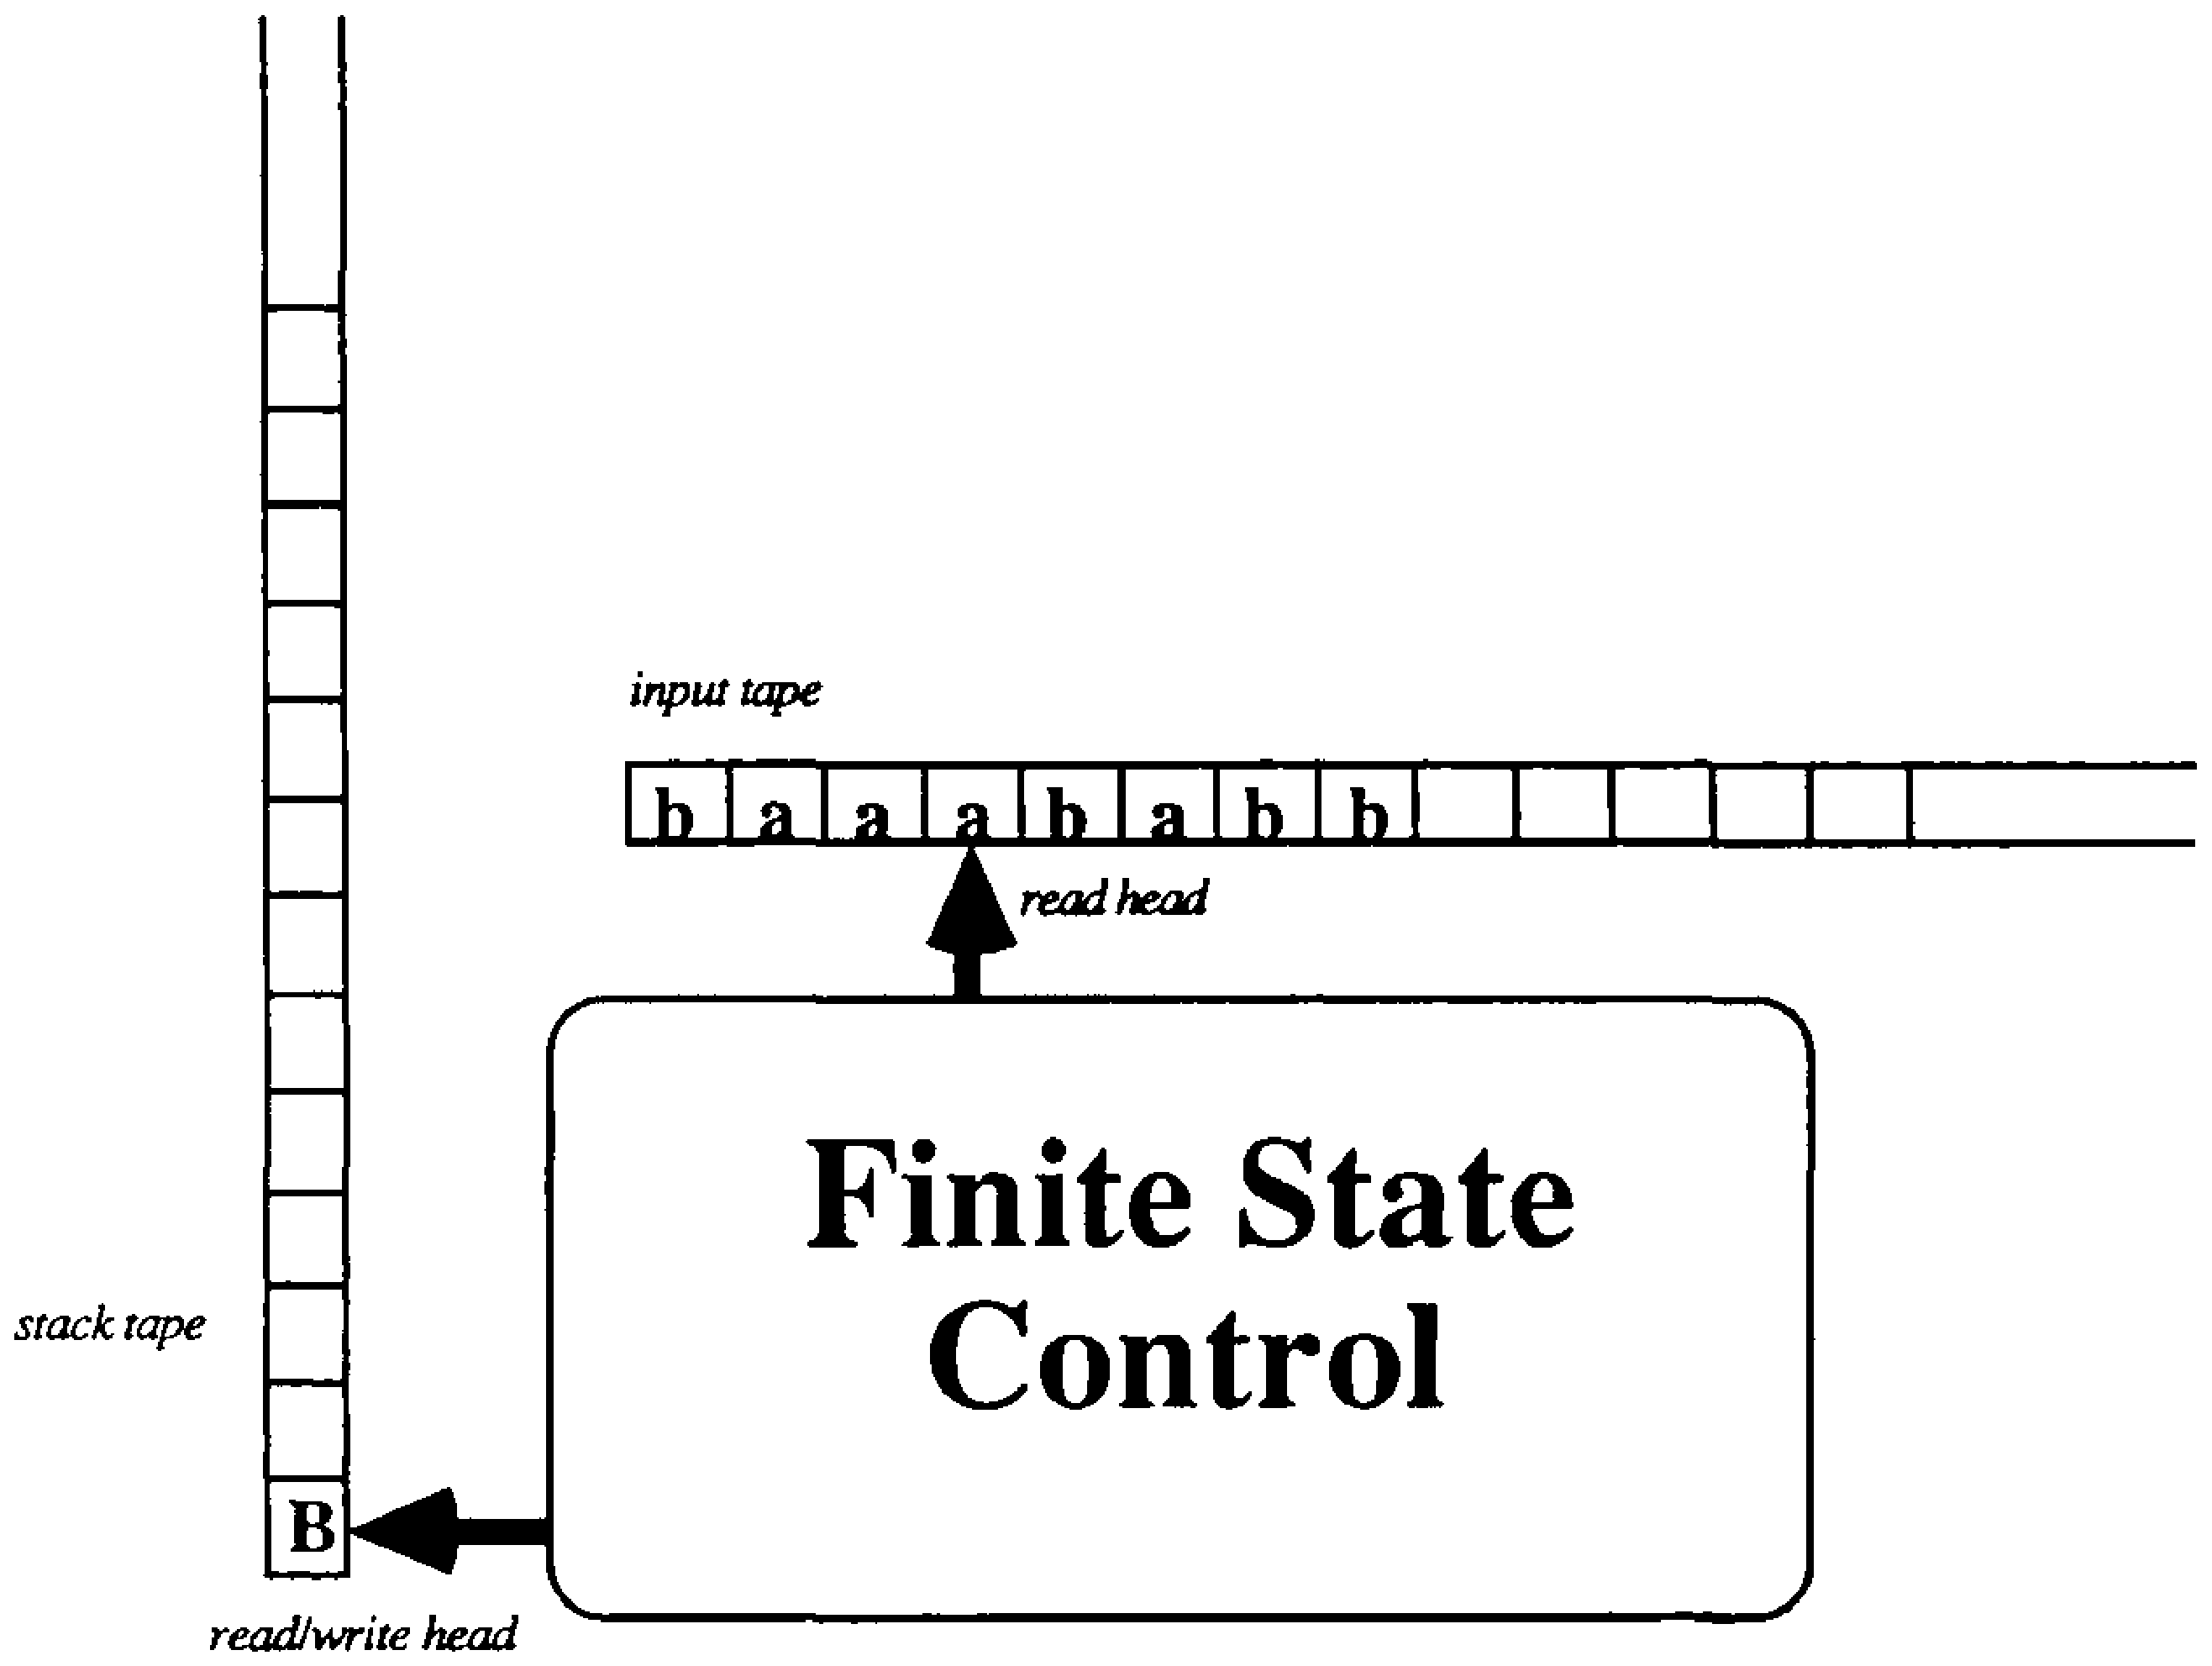
\epsfig{figure=ToFAfigures/fig10-1.eps,height=2.5in}}
\caption{A model of a pushdown automaton}\label{fig-10.1}
\end{figure}

The auxiliary tape\index{tape!auxiliary}\index{auxiliary tape of a PDA} is similar to that of a finite-state transducer; the second
component of the range of the state transition function in a pushdown automaton
specifies the string to be written on the stack tape. Thus, the functions
$\delta$ and $\omega$ of a FST are essentially combined in the $\delta$ function for
pushdown automata. The auxiliary tape differs from that of a FST in that the
current symbol from $\Gamma$ on the tape is sensed by the stack read/write head
and can affect the subsequent operation of the automaton. If no symbols are
written to tape during a transition, the tape head drops back one position and
will then be scanning the previous stack symbol. In essence, a state transition
is initiated by the currently scanned symbol on both the input tape and the
stack tape and begins with the stack symbol being popped from the stack; the
state transition is accompanied by a push operation, which writes a new string
of stack symbols on the stack tape. If several symbols are written, the
auxiliary read/write head will move ahead an appropriate amount, and the head
will be positioned over the last of the symbols written. Thus, if exactly one
symbol is written, the stack tape head does not move, and the effect is that the
old top-of-stack symbol is overwritten by the new symbol. When the empty string
is to be written, the effect is a pop followed by a push of no letters, and the
stack tape head retreats one position. If the only remaining stack symbol is
removed from the stack in this fashion, the stack tape head moves off the end
of the tape. It would then no longer be scanning a valid stack symbol, so no
further transitions are possible, and the device \emph{halts}.

It is possible to manipulate the stack and change states without consuming an
input letter, which is the intent of the $\lambda$-moves in the state transition
function. Since at most one symbol can be removed from the stack as a result of
a transition, $\lambda$-moves allow the stack to be shortened by several symbols
before the next input symbol is processed.

Acceptance can be defined by requiring the stack to be empty after the entire
input tape is consumed (as was the case with counting automata) or by requiring
that the automaton be in a final state after all the input is consumed. The
nondeterminism may allow the device to react to a given input string in several
distinct ways. As with NDFAs, the input word is considered accepted if at least
one of the possible reactions satisfies the criteria for acceptance. For a given
PDA, the set of words accepted by the empty stack criterion will likely differ
from the set of words accepted by the final state condition.

\subsection*{Example 10.1}

Consider the PDA defined by $P_1=\langle\{\pmb{a},\pmb{b}\},\{A,B\},\{q,r\},q,
\delta,B,\emptyset\rangle$, where $\delta$ is defined by
\begin{center}\begin{tabular}{r@{ = }l}
$\delta(q,\pmb{a},B)$ & $\{\langle q,A\rangle\}$ \\
$\delta(q,\pmb{a},A)$ & $\{\langle q,AA\rangle\}$ \\
$\delta(q,\pmb{b},B)$ & $\{\ \ \}$ \\
$\delta(q,\pmb{b},A)$ & $\{\langle r,\lambda\rangle\}$ \\
$\delta(r,\pmb{a},B)$ & $\{\ \ \}$ \\
$\delta(r,\pmb{a},A)$ & $\{\ \ \}$ \\
$\delta(r,\pmb{b},B)$ & $\{\ \ \}$ \\
$\delta(r,\pmb{b},A)$ & $\{\langle r,\lambda\rangle\}$
\end{tabular}\end{center}
Note that since the set of final states is empty no strings are accepted by
final state. We wish to consider the set of strings accepted by empty stack. In
general, when the set of final states is nonempty, the PDA will designate a
machine designed to accept by final state;\index{accept by final state} $F=\emptyset$ will generally be taken
as an indication that acceptance is to be by empty stack.\index{accept by empty stack}

The action of the state transition function can be displayed much like that of
finite-state transducers. Transition arrows are no longer labeled with just a
symbol from the input alphabet, since both a stack symbol and an input symbol
now govern the action of the automaton. Thus, arrows are labeled by ordered
pairs from $\Sigma\times\Gamma$. As with FSTs, this is followed by the output
caused by the transition. The diagram corresponding to $P_1$ is shown in Figure
\ref{fig-10.2}.

% Figure 10.2
\begin{figure}
\centerline{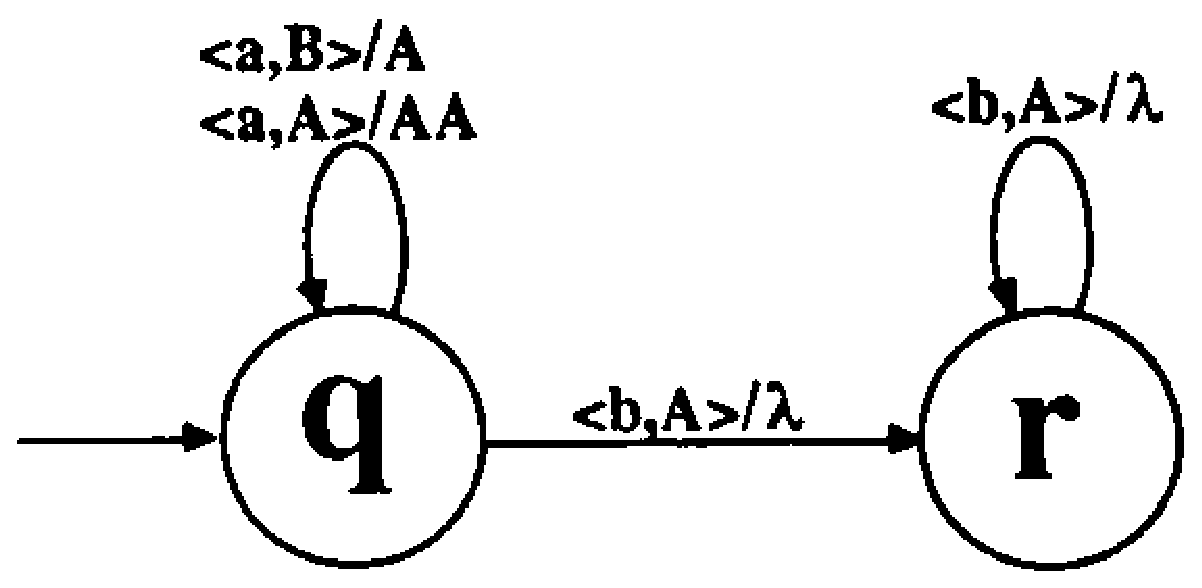
\epsfig{figure=ToFAfigures/fig10-2.eps,height=1in}}
\caption{The PDA discussed in Example 10.1}\label{fig-10.2}
\end{figure}

The reaction of $P_1$ to the string $\pmb{aabb}$ is the sequence of moves
displayed in Figures \ref{fig-10.3a}-e. Initially, the heads of the two tapes are positioned
as shown in Figure \ref{fig-10.3a}, with the (current) initial state highlighted. Since
the state is $q$, the input symbol is $\pmb{a}$, and the stack symbol is $B$, the
first transition rule $\delta(q,\pmb{a},B)=\{\langle q,A\rangle\}$ applies;
$P_1$ remains in state $q$, and the popped stack symbol $B$ is replaced by a
single $A$. Figure \ref{fig-10.3b} shows the new state of the automaton. The stack
read/write head is in the same position, since the length of the stack did not
change. The input read head moves on to the next letter, since the first input
symbol was consumed. The second rule now applies, and the single $A$ is replaced
by the pair $AA$ as $P_1$ returns to $q$ again, as shown in Figure \ref{fig-10.3c}. Note
that the stack tape head advanced as the topmost symbol was written. The rule
$\delta(q,\pmb{b},A)=\{\langle r,\lambda\rangle\}$ now applies, and the state
of the machine switches to $r$ as the (topmost) $A$ is popped and replaced with
an empty string, leaving the stack shorter than before. This is shown in Figure
\ref{fig-10.3d}. The last of the eight transition rules now applies, leaving the automaton
in the configuration shown by Figure \ref{fig-10.3e}. Since the stack is now empty, no
further moves are possible. However, since the read head has reached the end of
the input string, the word $\pmb{aabb}$ is accepted by $P_1$. The word $\pmb{aab}$
would be rejected by $P_1$ since the automaton would run out of input in a
configuration similar to that of Figure \ref{fig-10.3d}, in which the stack is not yet
empty. The word $\pmb{aabbb}$ would not be accepted because the stack would empty
prematurely, leaving $P_1$ stuck in a configuration similar to that of Figure
\ref{fig-10.3e}, but with the input string incompletely consumed. The word $\pmb{aaba}$
would likewise be rejected because there would be no move from the state $r$
with which to process the final input symbol $\pmb{a}$.

\setcounter{figure}{0}
\renewcommand{\thefigure}{\arabic{chapter}.3\alph{figure}}
% Figure 10.3a
\begin{figure}
\centerline{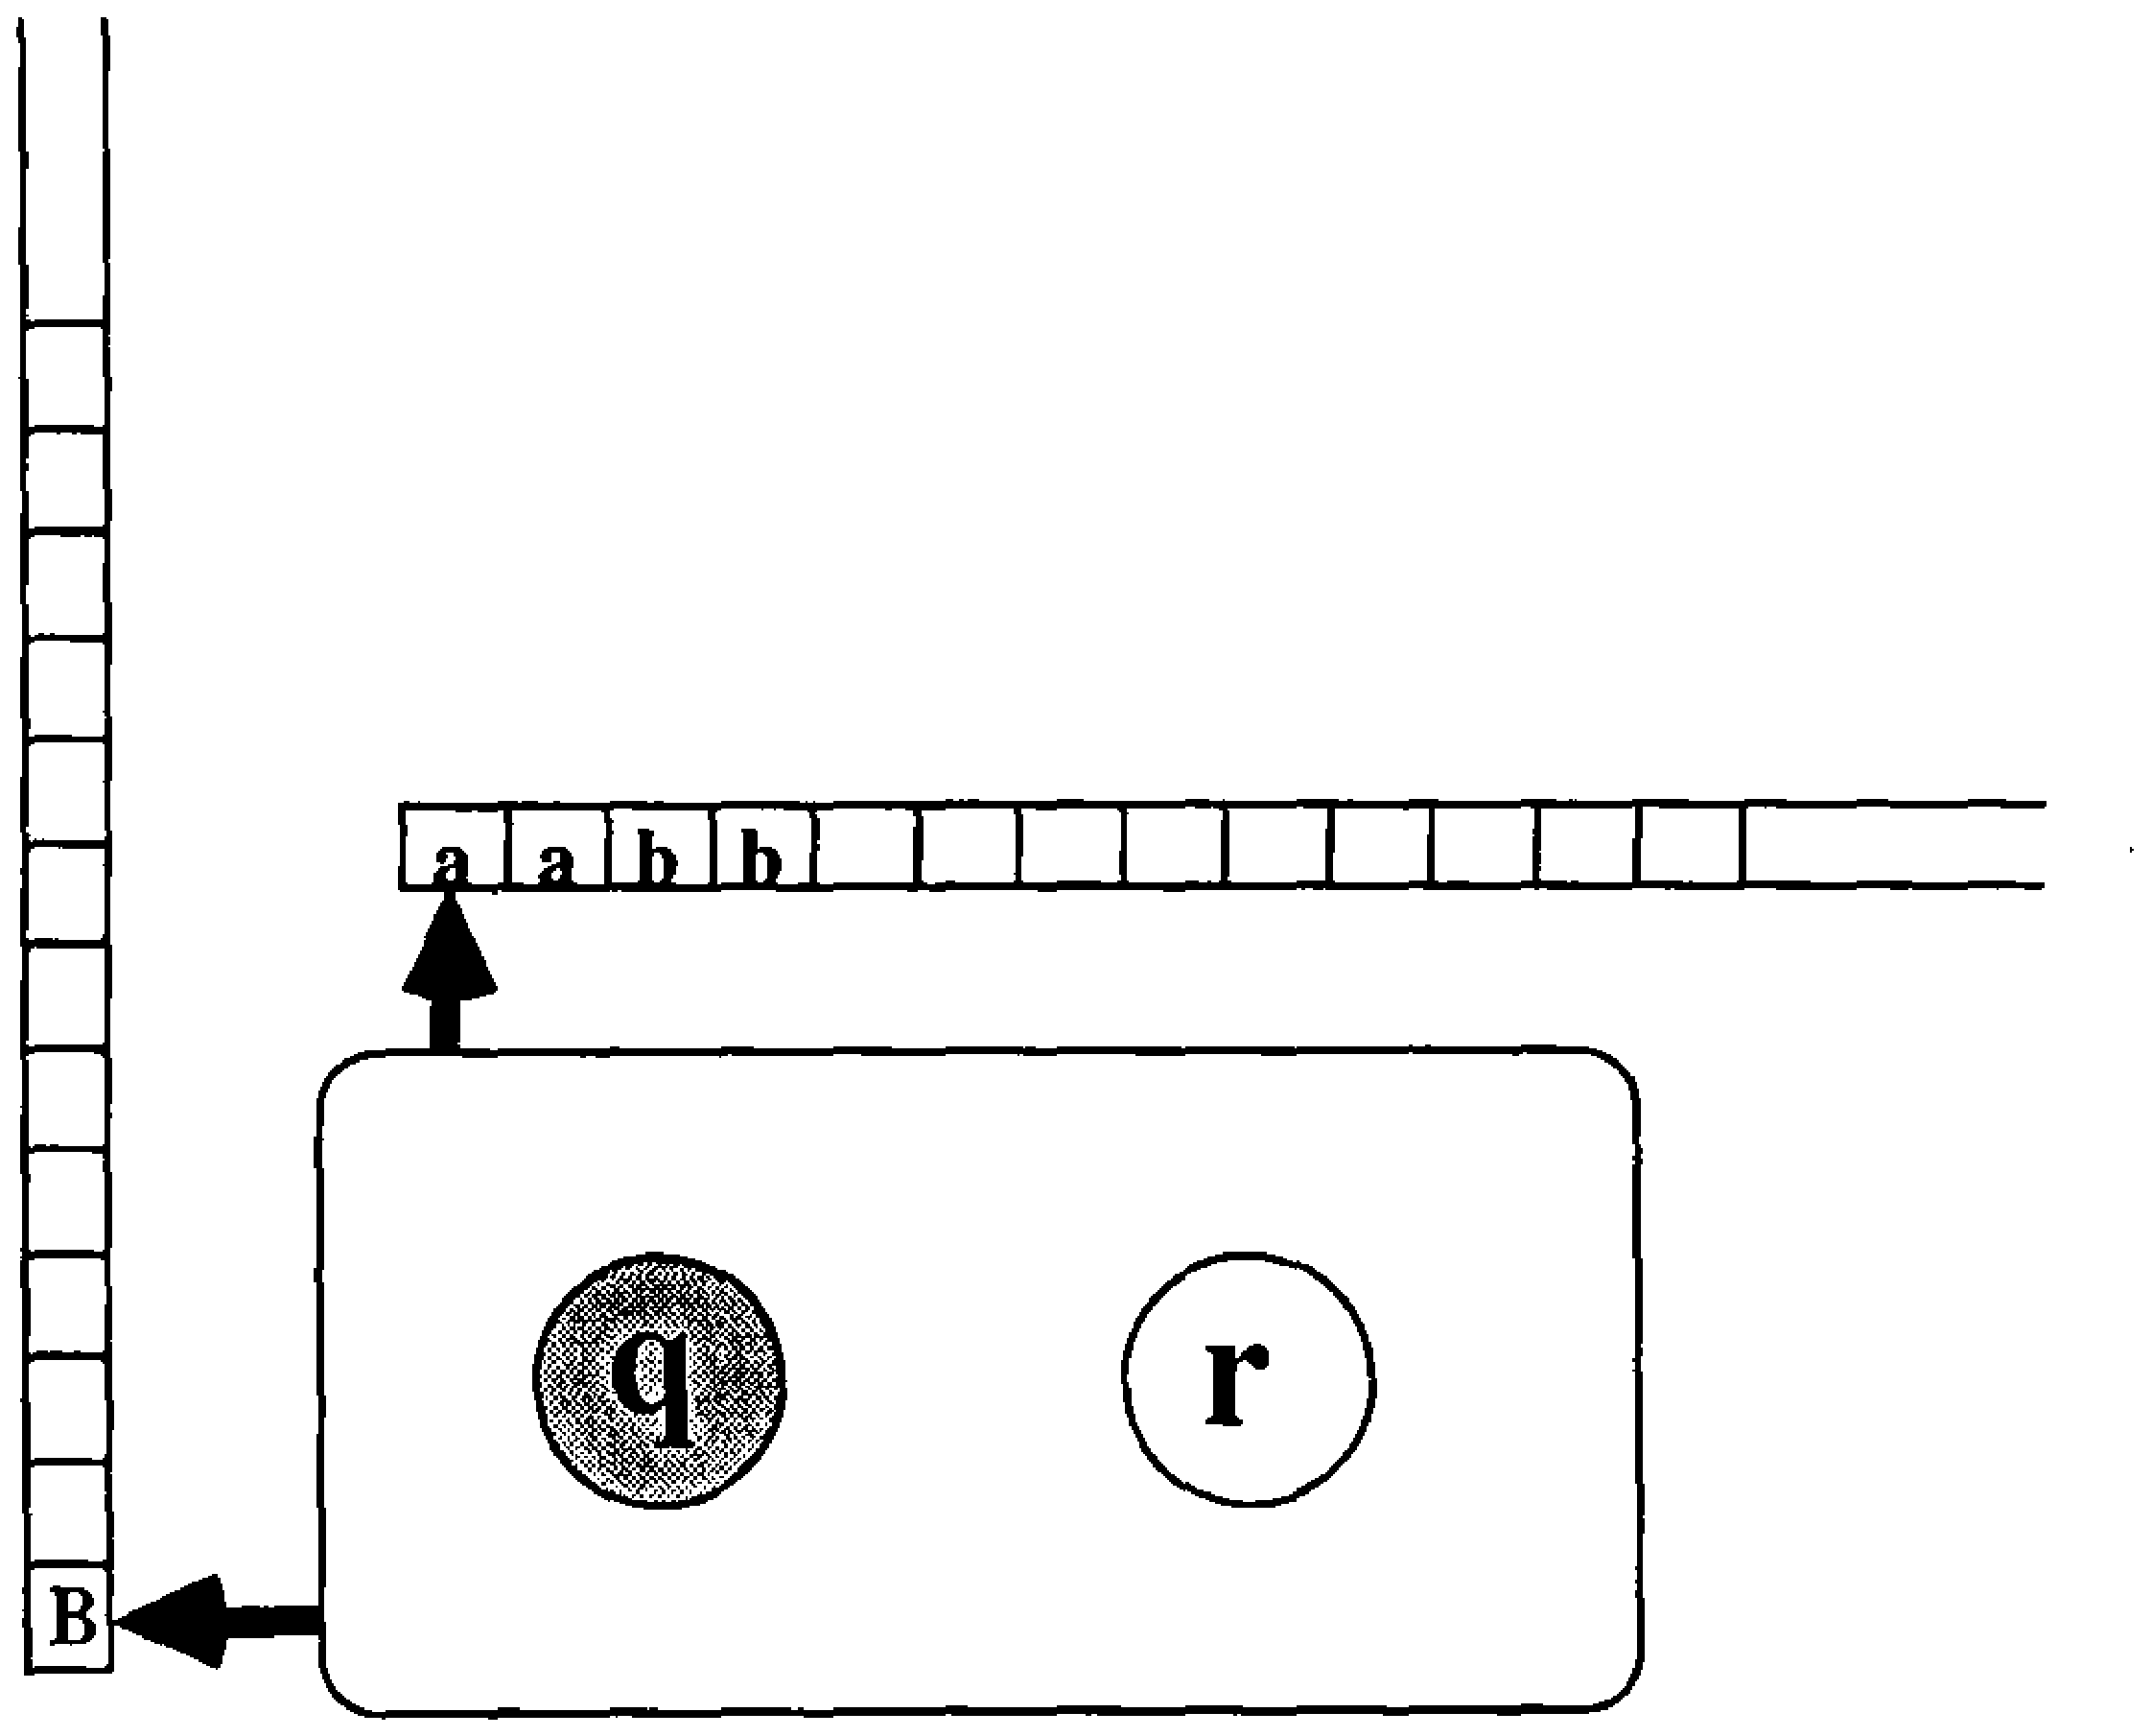
\epsfig{figure=ToFAfigures/fig10-3a.eps,height=2.0in}}
\caption{Walkthrough of the pushdown automaton discussed in Example 10.1}\label{fig-10.3a}
\end{figure}

% Figure 10.3b
\begin{figure}
\centerline{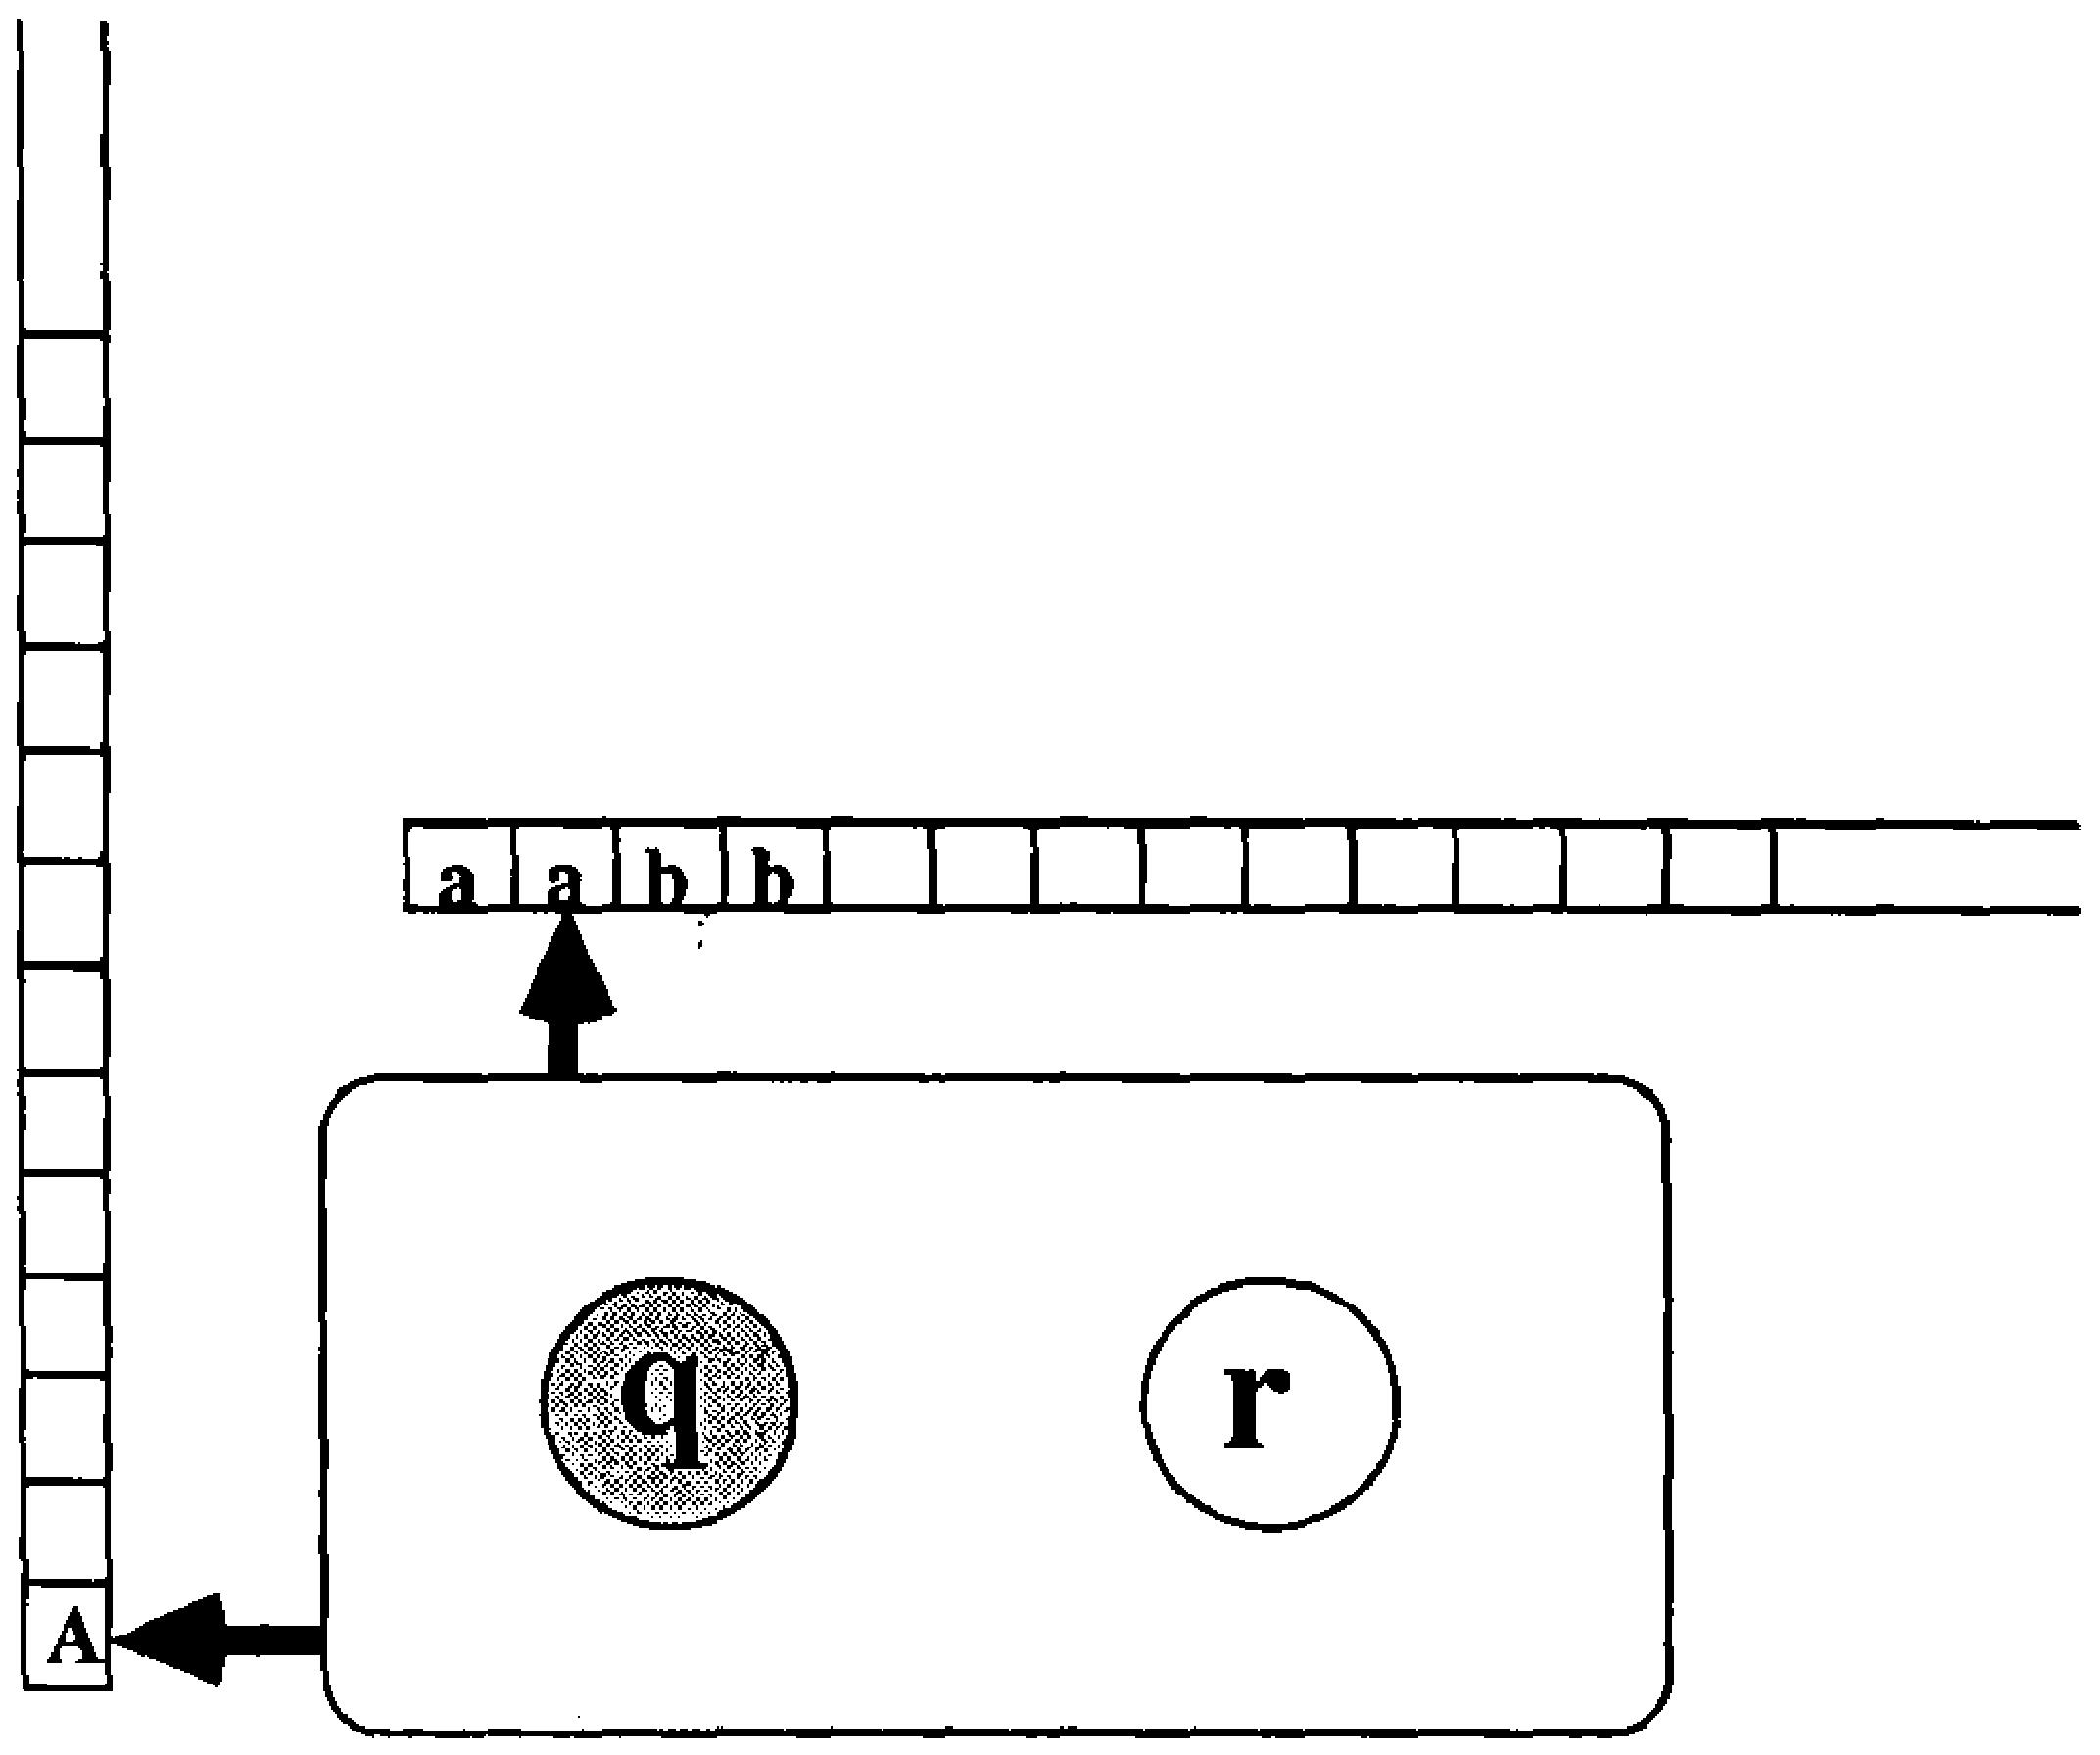
\epsfig{figure=ToFAfigures/fig10-3b.eps,height=2.0in}}
\caption{Walkthrough of the pushdown automaton discussed in Example 10.1}\label{fig-10.3b}
\end{figure}

% Figure 10.3c
\begin{figure}
\centerline{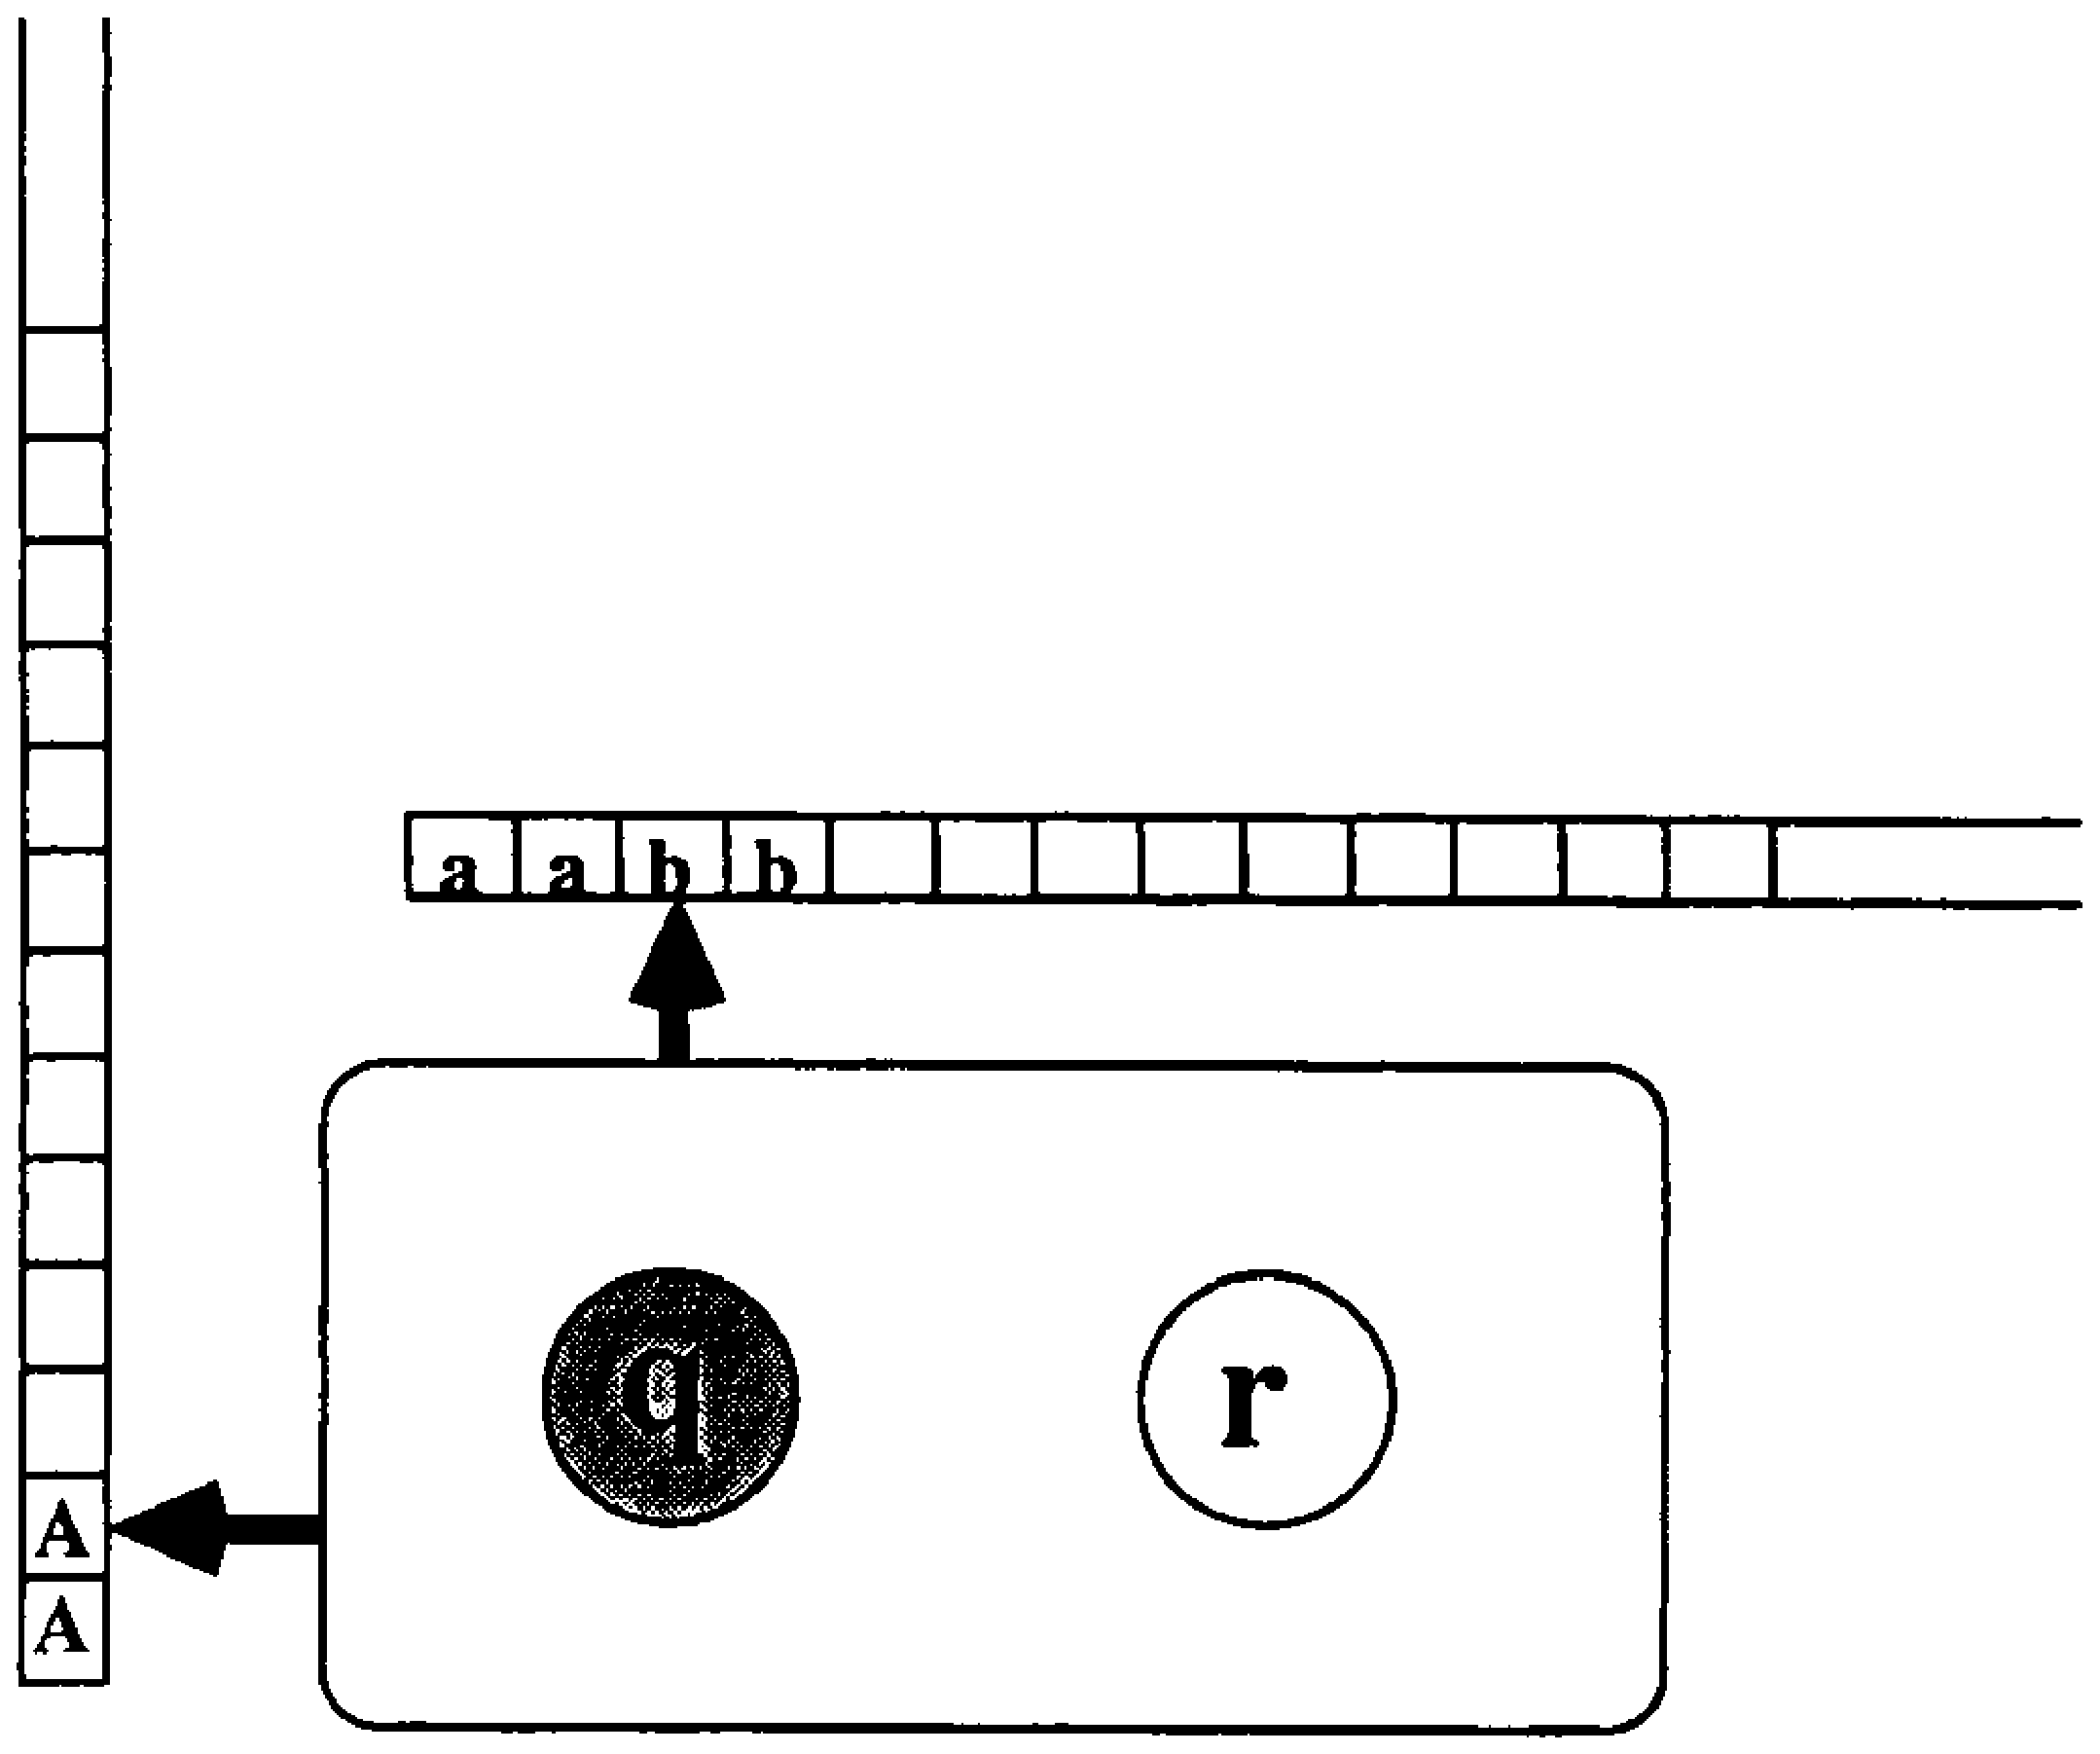
\epsfig{figure=ToFAfigures/fig10-3c.eps,height=2.0in}}
\caption{Walkthrough of the pushdown automaton discussed in Example 10.1}\label{fig-10.3c}
\end{figure}

% Figure 10.3d
\begin{figure}
\centerline{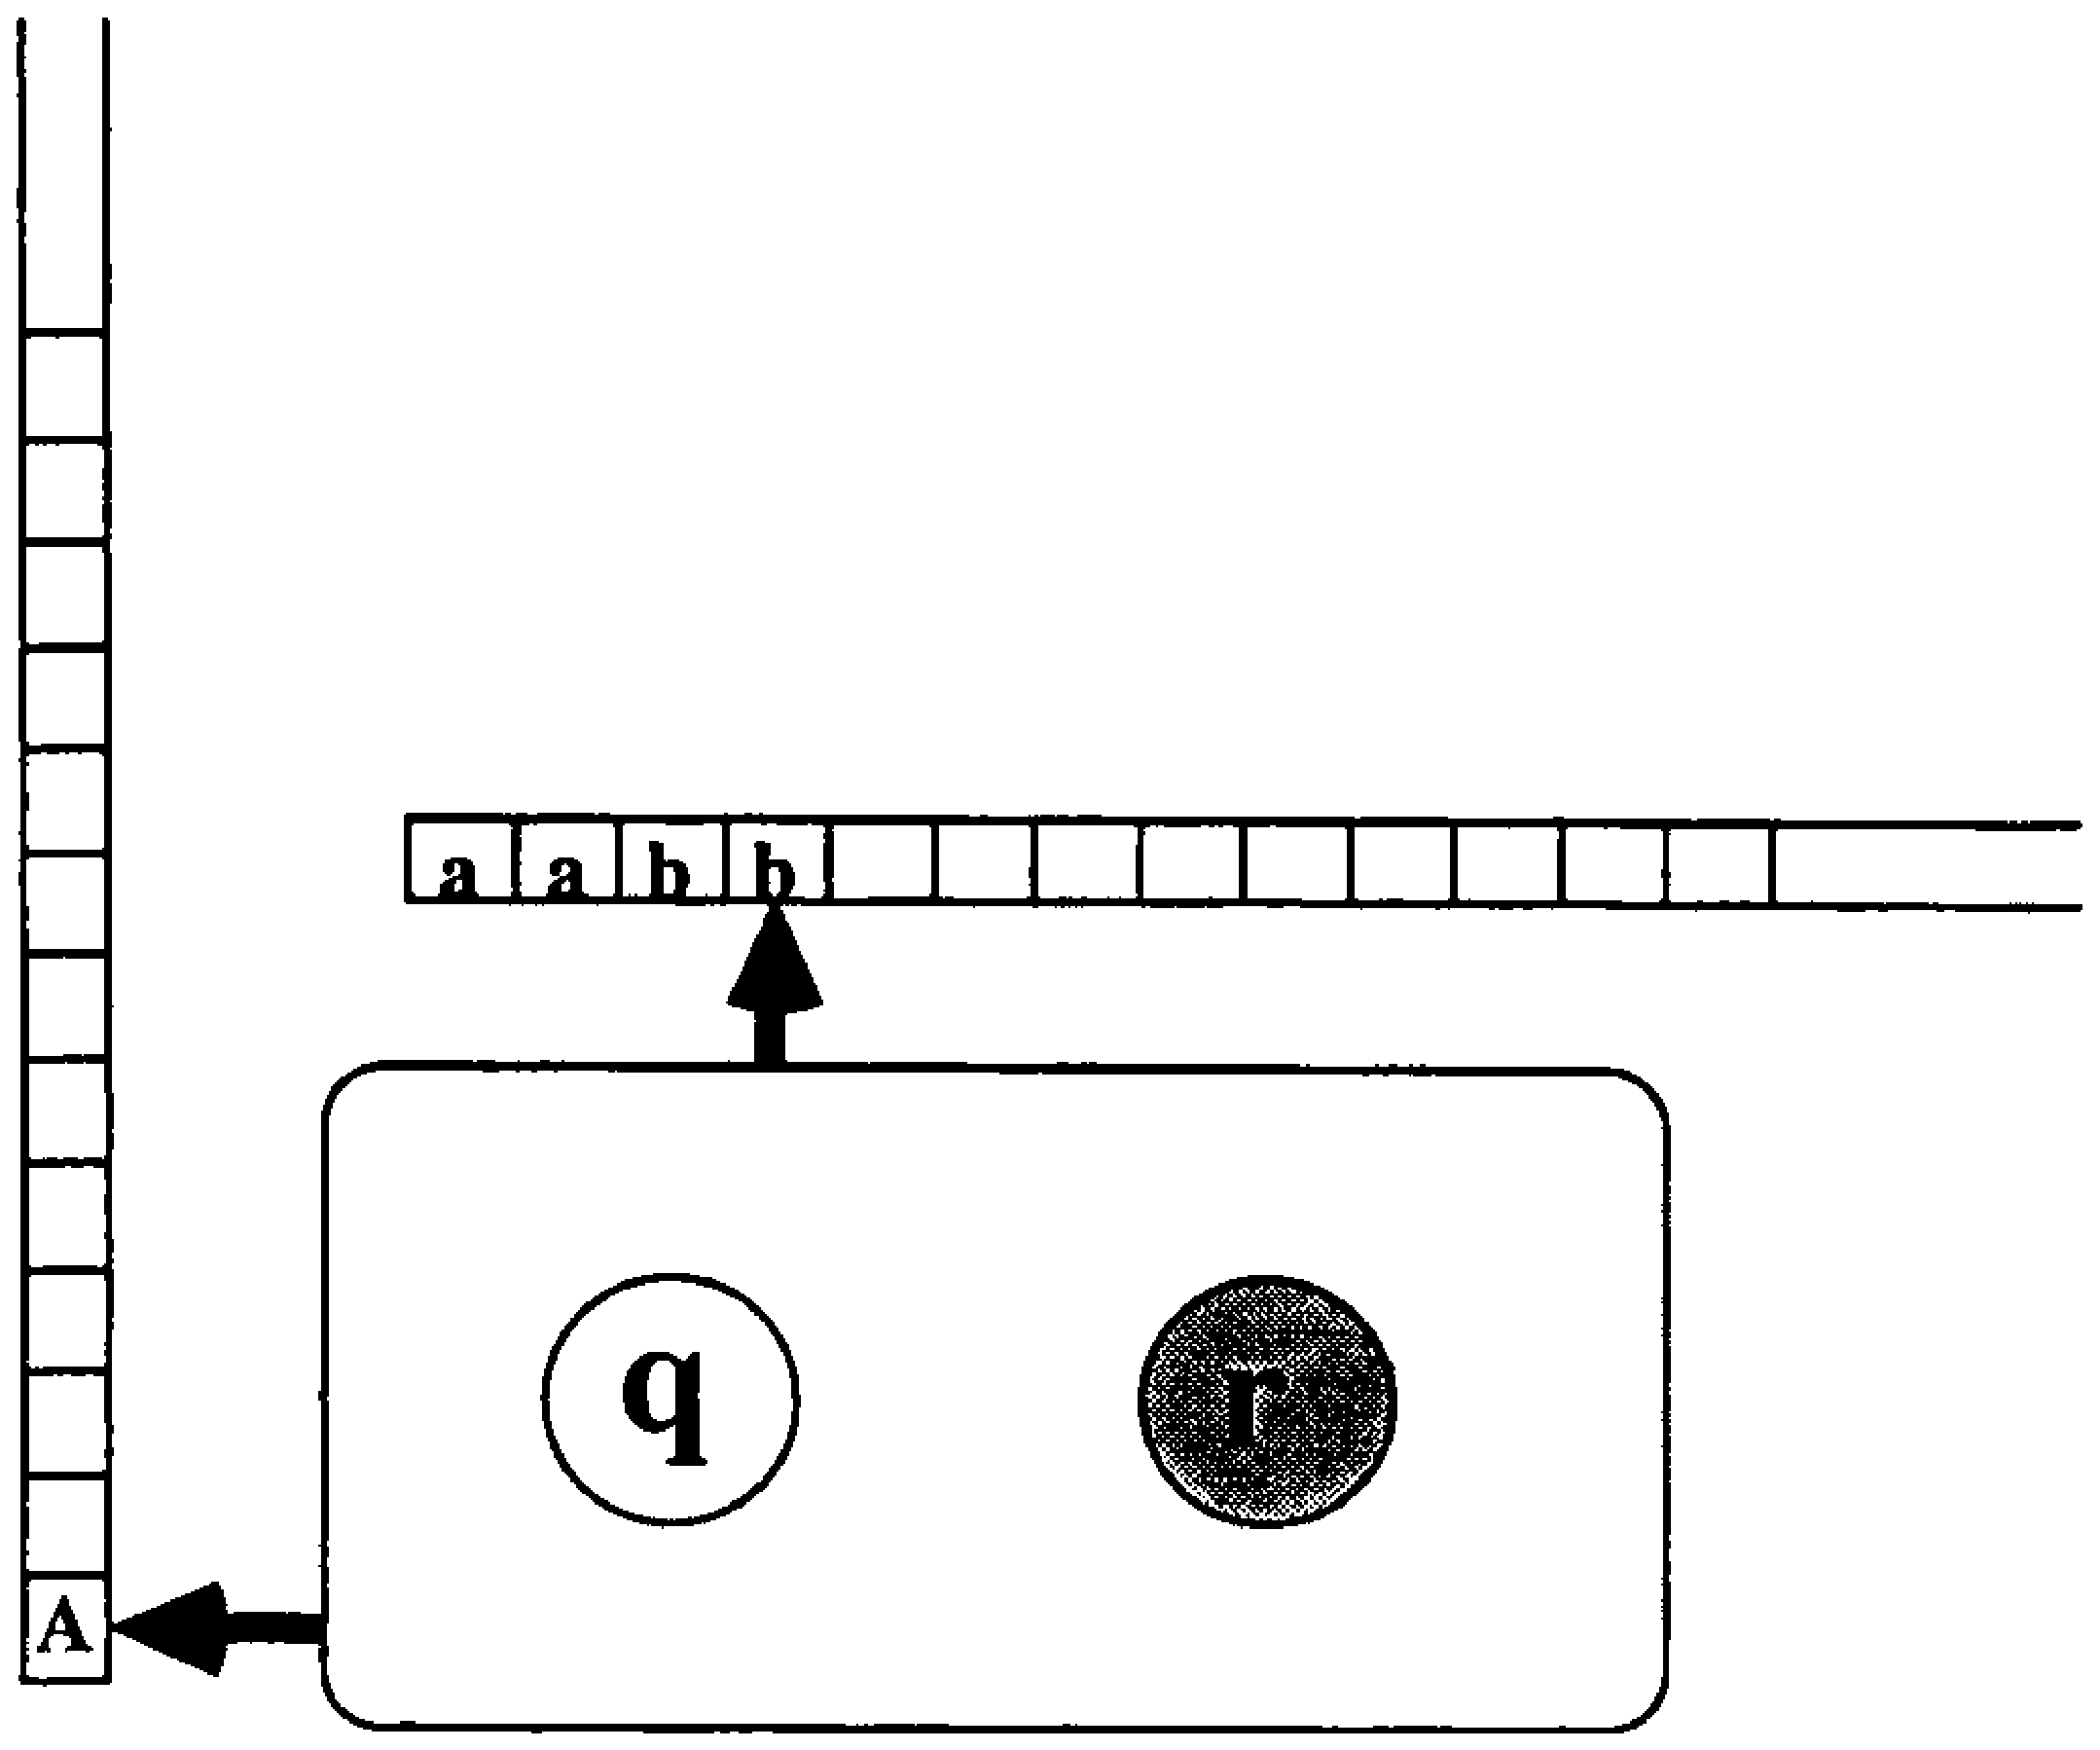
\epsfig{figure=ToFAfigures/fig10-3d.eps,height=2.0in}}
\caption{Walkthrough of the pushdown automaton discussed in Example 10.1}\label{fig-10.3d}
\end{figure}

% Figure 10.3e
\begin{figure}
\centerline{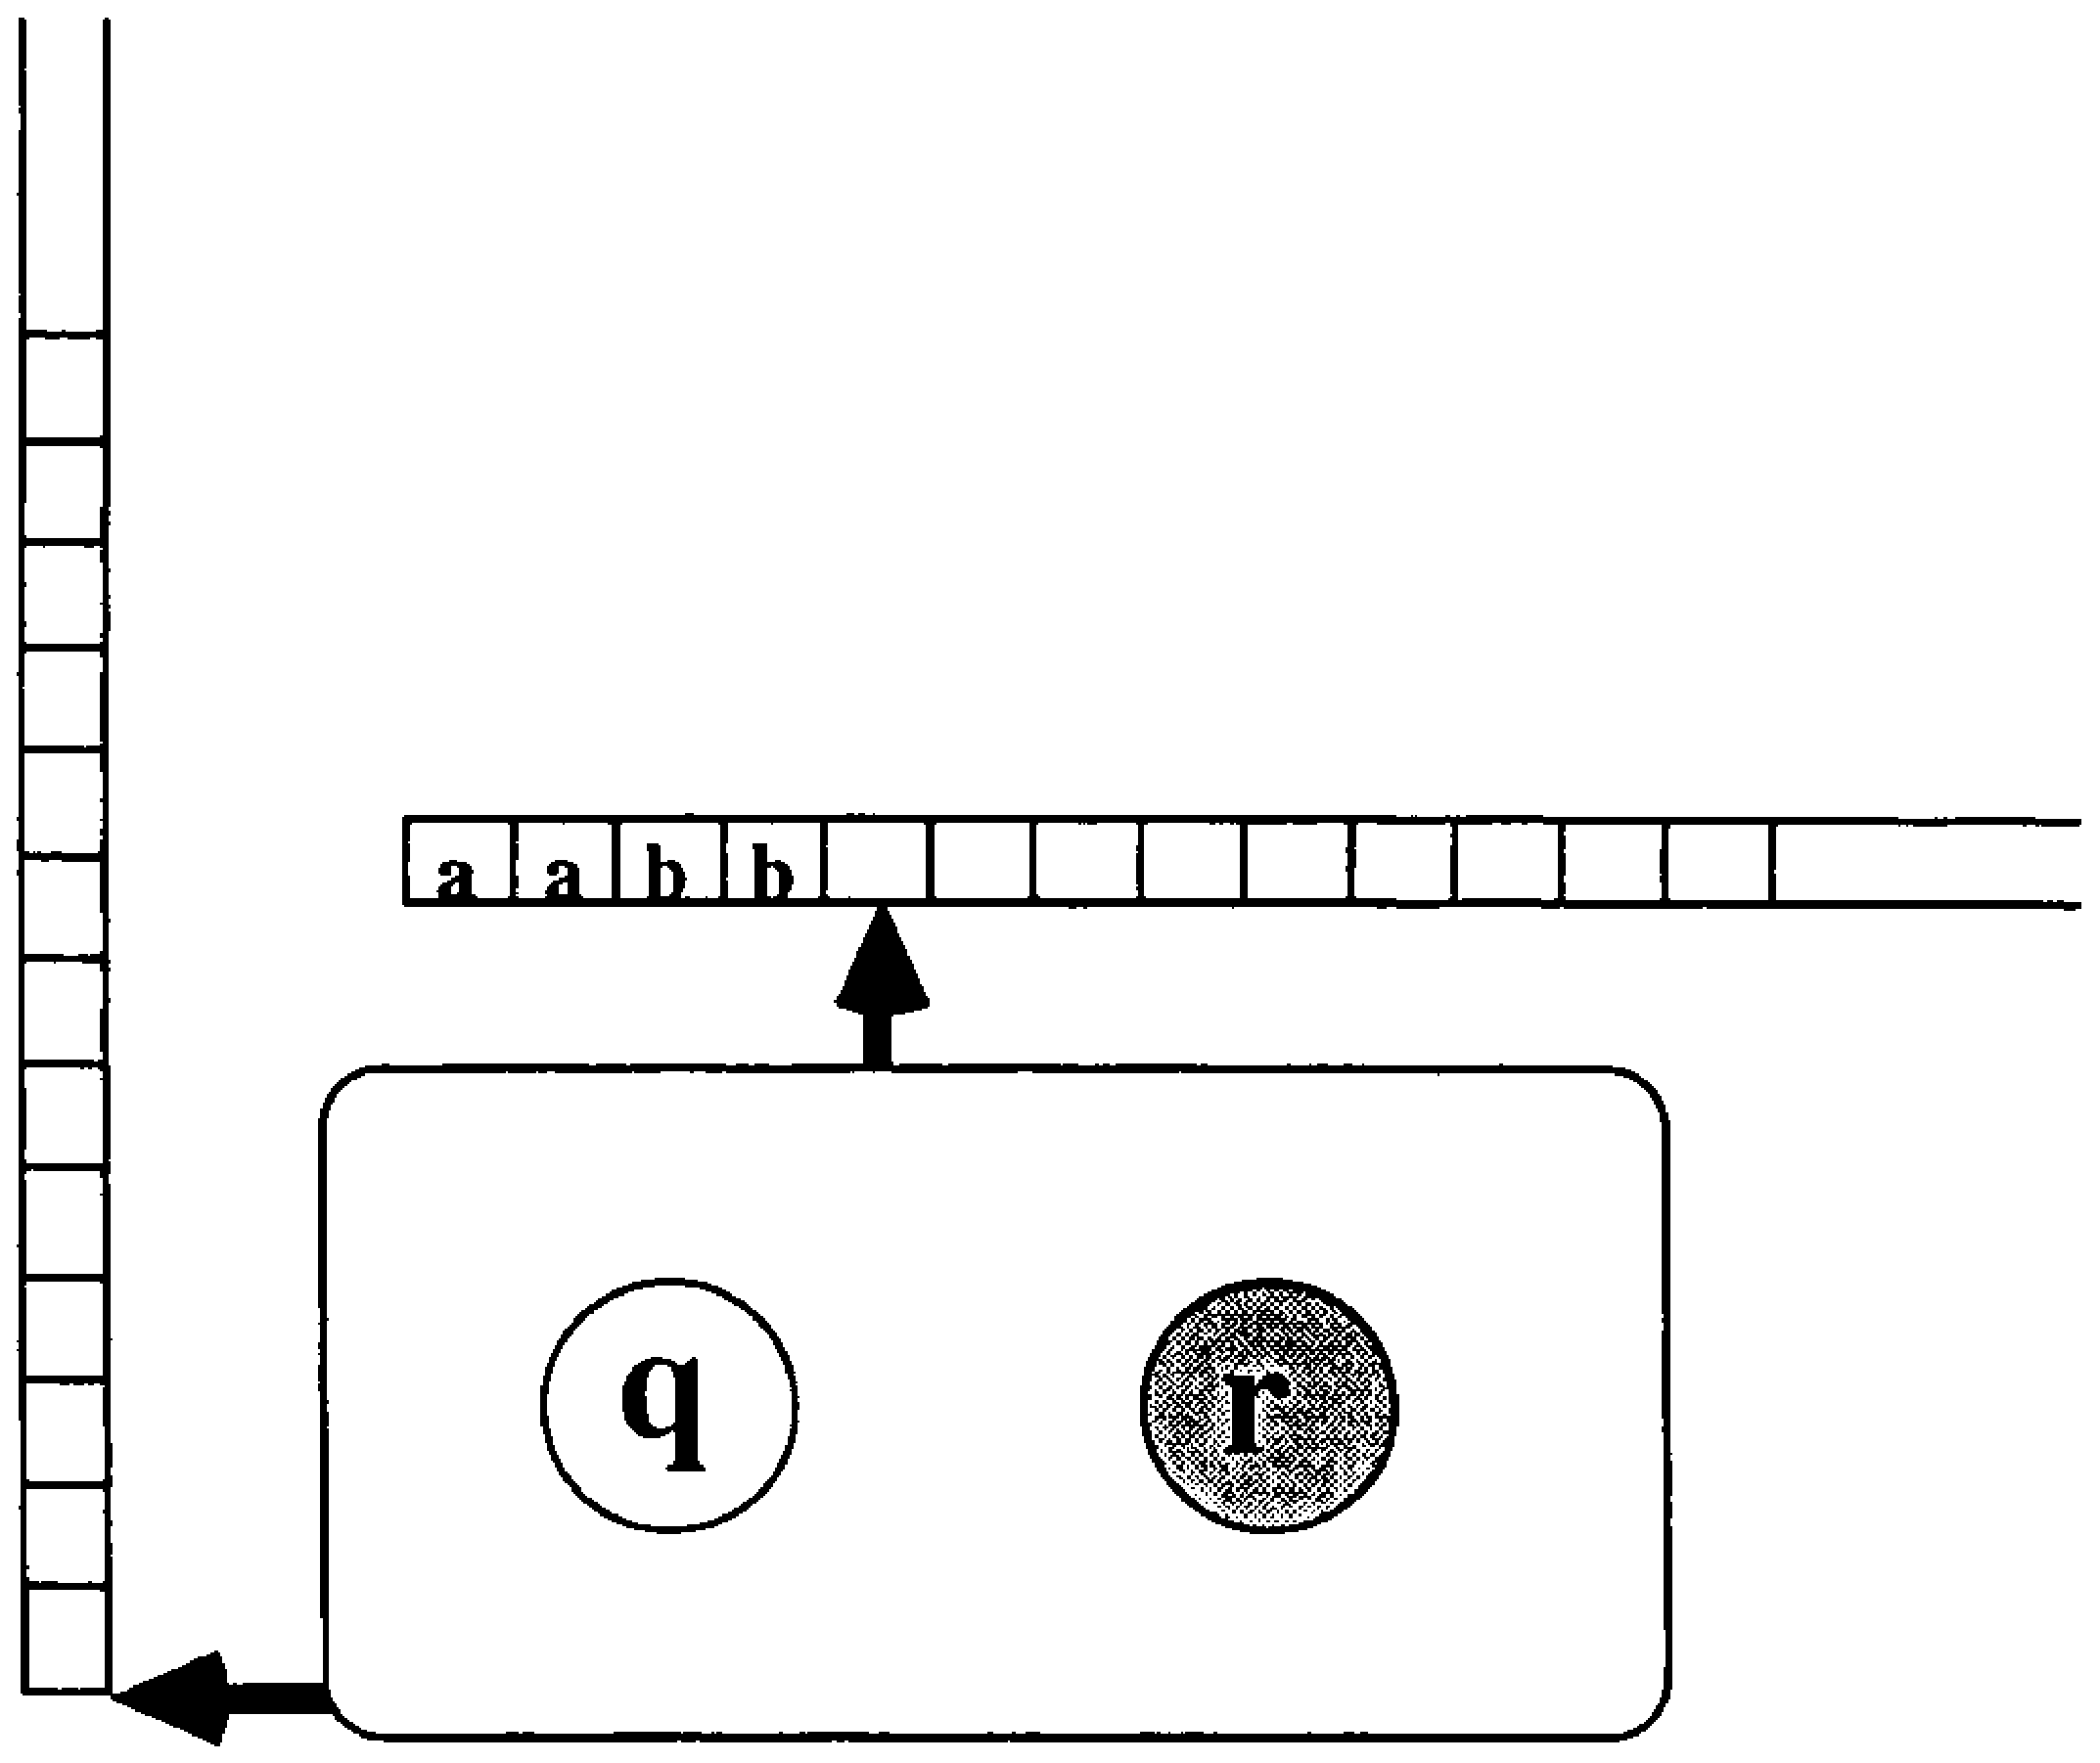
\epsfig{figure=ToFAfigures/fig10-3e.eps,height=2.0in}}
\caption{Walkthrough of the pushdown automaton discussed in Example 10.1}\label{fig-10.3e}
\end{figure}
\setcounter{figure}{3} %nasty kluge: latex thinks it's now up to figure 8, not 4
\renewcommand{\thefigure}{\arabic{chapter}.\arabic{figure}}

As with deterministic finite automata, once an input symbol is consumed, it has
no further effect on the operation of the pushdown automaton. The current state
of the device, the remaining input symbols, and the current stack contents form
a triple that describes the current configuration of the PDA. The triple
$\langle q,\pmb{bb},AA\rangle$ thus describes the configuration of the PDA in Figure
\ref{fig-10.3c}. When processing $\pmb{aabb}$, $P_1$ moved through the following sequence of
configurations:

\begin{center}\begin{tabular}{l}
$\langle q,\pmb{aabb},B\rangle$ \\
$\langle q,\pmb{abb},A\rangle$ \\
$\langle q,\pmb{bb},AA\rangle$ \\
$\langle r,\pmb{b},A\rangle$ \\
$\langle r,\lambda,\lambda\rangle$
\end{tabular}\end{center}
Successive configurations followed from their predecessors by applying a single
rule from the state transition function. These transitions will be described by
the operator $\vdash$.

% Definition 10.2
\begin{dfn}\label{dfn-10.2}
The current \emph{configuration} of pushdown automaton $P=\langle\Sigma,\Gamma,
S,s_0,\delta,B,F\rangle$ is described by a triple $\langle s,x,\alpha\rangle$,
where
\begin{quote}
$s$ is the current state. \\
$x$ is the unconsumed portion of the input string. \\
$\alpha$ is the current stack contents (with the topmost symbol written as the
leftmost).
\end{quote}

An ordered pair $\langle t,\gamma\rangle$ within the finite set of objects specified by
$\delta(s,\pmb{a},A)$ can cause a \emph{move} in the pushdown automaton $P$ from
the configuration $\langle s,\pmb{a}y,A\beta\rangle$ to the configuration $\langle t,y,\gamma\beta\rangle$.
This transition is denoted as $\langle s,\pmb{a}y,A\beta\rangle\vdash\langle t,y,\gamma\beta\rangle$.

A sequence of successive moves in which
\[ \langle s_1,x_1,\alpha_1\rangle\vdash\langle s_2,x_2,\alpha_2\rangle,\langle
	s_2,x_2,\alpha_2\rangle\vdash\langle s_3,x_3,\alpha_3\rangle,\ldots,
	\langle s_{m-1},x_{m-1},\alpha_{m-1}\rangle\vdash\langle s_m,x_m,
	\alpha_m\rangle \]
is denoted by $\langle s_1,x_1,\alpha_1\rangle\Dvdash\langle s_m,x_m,\alpha_m\rangle$.
\end{dfn}
The operator\ $\Dvdash$\ reflects the reflexive and transitive closure of $\vdash$,
and thus we also have $\langle s_1,x_1,\alpha_1\rangle\Dvdash\langle s_1,x_1,\alpha_1\rangle$ and clearly
$\langle s_1,x_1,\alpha_1\rangle\vdash\langle s_2,x_2,\alpha_2\rangle$ implies $\langle s_1,x_1,\alpha_1\rangle\Dvdash
\langle s_2,x_2,\alpha_2\rangle$.

\subsection*{Example 10.2}

For the pushdown automaton $P_1$ in Example 10.1, $\langle q,\pmb{aabb},B\rangle
\Dvdash\langle r,\lambda,\lambda\rangle$ because $\langle q,\pmb{aabb},B\rangle
\vdash\langle q,\pmb{abb},A\rangle\vdash\langle q,\pmb{bb},AA\rangle\vdash
\langle r,\pmb{b},A\rangle\vdash\langle r,\lambda,\lambda\rangle$.

% Definition 10.3
\begin{dfn}\label{dfn-10.3}\index{language!accepted by final state PDA}\index{language!accepted by empty stack PDA}
For a pushdown automaton $P=\langle\Sigma,\Gamma,S,s_0,\delta,B,F\rangle$, the
\emph{language accepted via final state} by $P$, $L(P)$, is
\[ \{x\in\Sigma^*|\ \exists r\in F,\exists\alpha\in\Gamma^*\ni\langle s_0,x,B
	\rangle\Dvdash\langle r,\lambda,\alpha\rangle\} \]
\emph{The language accepted via empty stack} by $P$, $\Lambda(P)$, is
\[ \{x\in\Sigma^*|\ \exists r\in S\ni\langle s_0,x,B\rangle\Dvdash\langle r,
	\lambda,\lambda\rangle\} \]
\end{dfn}

\subsection*{Example 10.3}

Consider the pushdown automaton $P_1$ in Example 10.1. Since only strings of the
form $\pmb{a}^i\pmb{b}^i$ (for $i \geq 1$) allow $\langle q,\pmb{a}^i\pmb{b}^i,
B\rangle\Dvdash\langle r,\lambda,\lambda\rangle$, it follows that $\Lambda(P_1)
=\{\pmb{a}^n\pmb{b}^n|\ n\geq 1\}$. However, $F=\emptyset$ and thus $L(P_1$) is
clearly $\emptyset$.

The pushdown automaton $P_1$ in Example 10.1 was \emph{deterministic} in the
sense that there will never be more than one choice that can be made from any
configuration. The following example illustrates a pushdown automaton that is
nondeterministic.

\subsection*{Example 10.4}

Consider the pushdown automaton defined by $P_2=\langle\{\pmb{a},\pmb{b}\},\{S,
C\},\{t\},t,\delta,S,\emptyset\rangle$, where $\delta$ is defined by
\begin{center}\begin{tabular}{r@{ = }l}
$\delta(t,\pmb{a},S)$ & $\{\langle t,SC\rangle,\langle t,C\rangle\}$ \\
$\delta(t,\pmb{a},C)$ & $\{\ \ \}$ \\
$\delta(t,\pmb{b},S)$ & $\{\ \ \}$ \\
$\delta(t,\pmb{b},C)$ & $\{\langle t,\lambda\rangle\}$ \\
$\delta(t,\lambda,S)$ & $\{\ \ \}$ \\
$\delta(t,\lambda,C)$ & $\{\ \ \}$
\end{tabular}\end{center}
In this automaton, there are two distinct courses of action when the input
symbol is $\pmb{a}$ and the top stack symbol is $S$, which leads to several
possible options when trying to process the word $\pmb{aabb}$. One option is to
apply the first move whenever possible, which leads to the sequence of
configurations
\[ \langle t,\pmb{aabb},S\rangle\vdash\langle t,\pmb{abb},SC\rangle\vdash\langle
	t,\pmb{bb},SCC\rangle. \]
Since there are no $\lambda$-moves and $\delta(t,\pmb{b},S)=\{\ \ \}$, there are
no further moves that can be made, and the input word cannot be completely
consumed in this manner. Another option is to choose the second move option
exclusively, leading to the abortive sequence $\langle t,\pmb{aabb},S\rangle
\vdash\langle t,\pmb{abb},C\rangle$; $\delta(t,\pmb{a},C)=\{\ \ \}$, and
processing again cannot be completed. A mixture of the first and second moves
results in the sequence $\langle t,\pmb{aabb},S\rangle\vdash\langle t,\pmb{abb},
SC\rangle\vdash\langle t,\pmb{bb},CC\rangle\vdash\langle t,\pmb{b},C\rangle
\vdash\langle t,\lambda,\lambda\rangle$, and $\pmb{aabb}$ is thus accepted by
$P_2$. Further experimentation shows that $\Lambda(P_2)=\{\pmb{a}^n\pmb{b}^n|\ n
\geq 1\}$. To successfully empty its stack, this automaton must correctly
``guess'' when the last $\pmb{a}$ is being read and choose the second transition
pair, placing only $C$ on the stack.

% Definition 10.4
\begin{dfn}\label{dfn-10.4}\index{equivalent!PDAs}
Two pushdown automata $M_1=\langle\Sigma,\Gamma_1,S_1,s_{0_1},\delta_1,B_1,F_1
\rangle$ and $M_2=\langle\Sigma,\Gamma_2,S_2,s_{0_2},\delta_2,\\ B_2,F_2\rangle$
are called \emph{equivalent} iff they accept the same language.
\end{dfn}

The pushdown automaton $P_1$ from Example 10.1 is therefore equivalent to $P_2$
in Example 10.4. The concept of equivalence will apply even if one device
accepts via final state and the other accepts via empty stack. In keeping with
the previous broad use of the concept of equivalence, if any two finite
descriptors define the same language, those descriptors will be called
equivalent. Thus, if a PDA $M$ happens to accept the language described by a
regular expression $R$, we will say that $R$ is equivalent to $M$.

\subsection*{Example 10.5}

The following pushdown automaton illustrates the use of $\lambda$-moves and
acceptance by final state for the language $\{\pmb{a}^n\pmb{b}^m|\ n\geq 1\wedge
(n=m \vee n=2m)\}$. Let $P_3=\langle\{\pmb{a},\pmb{b}\},\{A\},\{s_0\},\{s_0,s_1,
s_2,s_3,s_4\},\delta,A,\{s_2,s_4\}\rangle$, where $\delta$ is defined by
\begin{center}\begin{tabular}{r@{ = }l}
$\delta(s_0,\pmb{a},A)$ & $\{\langle s_0,AA\rangle\}$ \\
$\delta(s_0,\pmb{b},A)$ & $\{\ \ \}$ \\
$\delta(s_0,\lambda,A)$ & $\{\langle s_1,\lambda\rangle,\langle s_3,\lambda
	\rangle\}$ \\
$\delta(s_1,\pmb{a},A)$ & $\{\ \ \}$ \\
$\delta(s_1,\pmb{b},A)$ & $\{\langle s_1,\lambda\rangle\}$ \\
$\delta(s_1,\lambda,A)$ & $\{\langle s_2,\lambda\rangle\}$ \\
$\delta(s_2,\pmb{a},A)$ & $\{\ \ \}$ \\
$\delta(s_2,\pmb{b},A)$ & $\{\ \ \}$ \\
$\delta(s_2,\lambda,A)$ & $\{\ \ \}$ \\
$\delta(s_3,\pmb{a},A)$ & $\{\ \ \}$ \\
$\delta(s_3,\pmb{b},A)$ & $\{\ \ \}$ \\
$\delta(s_3,\lambda,A)$ & $\{\langle s_4,\lambda\rangle\}$ \\
$\delta(s_4,\pmb{a},A)$ & $\{\ \ \}$ \\
$\delta(s_4,\pmb{b},A)$ & $\{\langle s_3,\lambda\rangle\}$ \\
$\delta(s_4,\lambda,A)$ & $\{\ \ \}$
\end{tabular}\end{center}
The finite-state control for this automaton is diagrammed in Figure \ref{fig-10.4}. Note
that the $\lambda$-move from state $s_3$ is \emph{not} responsible for any
nondeterminism in this machine. From $s_3$, only one move is permissible: the
$\lambda$-move to $s_4$. On the other hand, the $\lambda$-move from state $s_1$
does allow a choice of moving to $s_2$ (without moving the read head) or staying
at $s_1$ while consuming another input symbol. The choice of moves from state
$s_0$ also contributes to the nondeterminism; the device must ``guess'' whether
the number of $\pmb{b}$s will equal the number of $\pmb{a}$s or whether there will
be half as many, and at the appropriate time transfer control to $s_1$ or $s_3$,
respectively. Notice that the moves defined by states $s_3$ and $s_4$ allow
\emph{two} stack symbols to be removed for each $\pmb{b}$ consumed. Furthermore, a
string like $\pmb{aab}$ can transfer control to $s_3$ as the final $\pmb{b}$ is
processed, but the $\lambda$-move can then be applied to reach $s_4$ even though
there are no more symbols on the input tape.

% Figure 10.4
\begin{figure}
\centerline{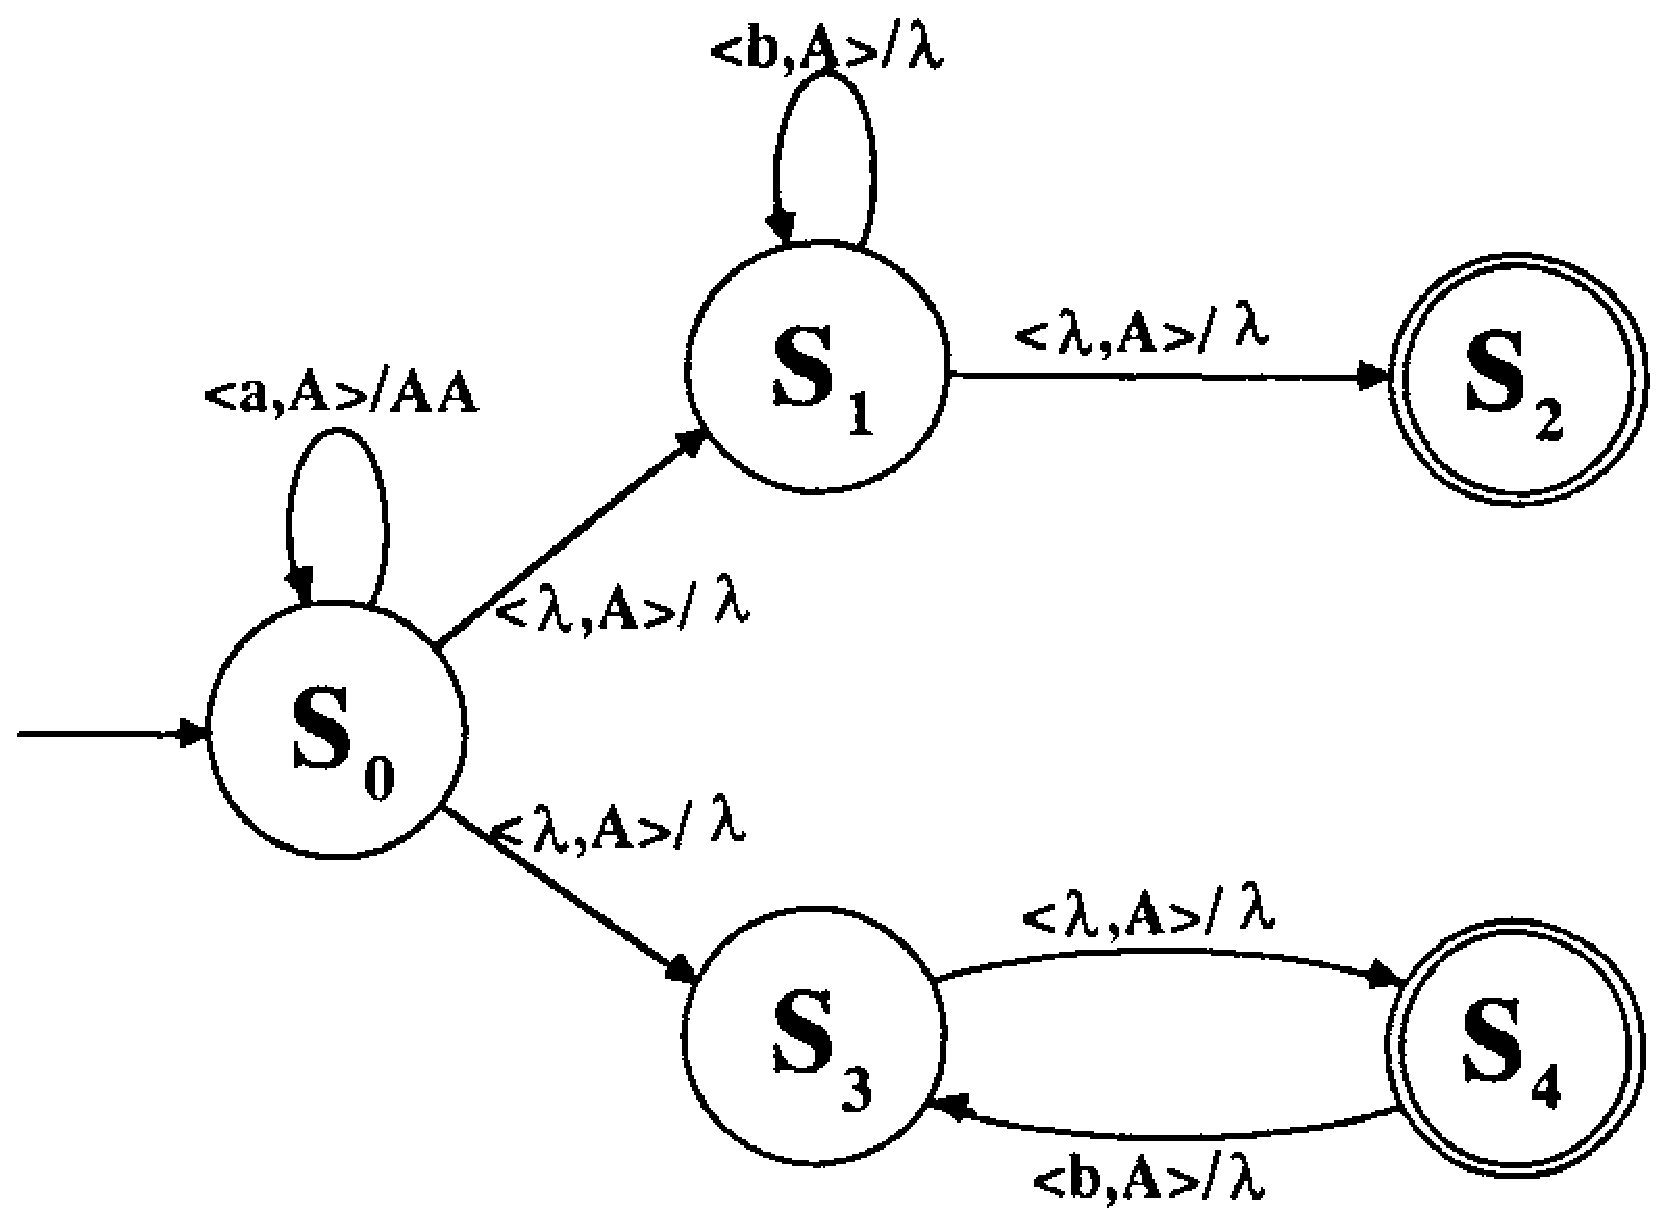
\epsfig{figure=ToFAfigures/fig10-4.eps,height=3.0in}}
\caption{The PDA discussed in Example 10.5}\label{fig-10.4}
\end{figure}

Since $A$ was the only stack symbol in $P_3$, the language could have as easily
been described by the sack-and-stone counting device described at the beginning
of the section. It should be clear that counting automata are essentially
pushdown automata with a singleton stack alphabet. Pushdown automata with only
one stack symbol cannot generate all the languages that a PDA with two symbols
can [DENN]. However, it can be shown that using more than two stack symbols does
not contribute to the generative power of a PDA; for example, a PDA with
$\Gamma=\{A,B,C,D\}$ can be converted into an equivalent machine with $\Gamma'=
\{0,1\}$ and the occurrences of the old stack symbols replaced by the encodings
$A=01,\ B=001,\ C=0001$, and $D=00001$.

Every NDFA can be simulated by a PDA that simply ignores its stack. In fact,
every NDFA has an equivalent counting automaton, as shown in the following
theorem.

% Theorem 10.1
\begin{thm}\label{thm-10.1}\index{equivalent!PDAs}\index{NDFA}
Given any alphabet $\Sigma$, and an NDFA $A$:
\begin{enumerate}
\item There is an equivalent pushdown automaton (counting automaton) $A'$ for
which $L(A)=L(A')$.
\item There is an equivalent pushdown automaton (counting automaton) $A''$ for
which $L(A)=\Lambda(A'')$.
\end{enumerate}

\emph{Proof.} The results for pushdown automata will actually follow from the
results of the next section, since pushdown automata can define all the
context-free languages, and the regular language defined by the NDFA $A$ must be
context free. The following constructions will use only the one stack symbol
\cent, and hence $A'$ and $A''$ are actually \emph{counting} automata for which $L(A)=
L(A')$ and $L(A)=\Lambda(A'')$.

While the construction of a PDA from an NDFA is straightforward, the inductive
proofs are simplified if we appeal to Theorem \ref{thm-4.1}, and assume that the given
automaton is actually a DFA $A=\langle\Sigma,S,s_0,\delta,F\rangle$. Define the
PDA $A'=\langle\Sigma,\{\cent\},S,s_0,\delta',\cent,F\rangle$, where $\delta'$
is defined by
\[ (\forall s\in S)(\forall \pmb{a}\in\Sigma)(\delta'(s,\pmb{a},\cent)=\{\langle
	\delta(s,\pmb{a}),\cent\rangle\}) \]
and $(\forall s\in S)(\delta'(s,\lambda,\cent)=\{\ \ \})$. That is, the PDA makes
the same transitions that the DFA does and replaces the \cent\ with the same
symbol on the stack at each move. The proof that $A$ and $A'$ are equivalent is
by induction on the length of the input string, where $P(n)$ is the statement
that
\[ (\forall x\in\Sigma^n)(\DBAR(s_0,x)=t\Leftrightarrow\langle s_0,x,\cent
	\rangle\Dvdash\langle t,\lambda,\cent\rangle) \]
The PDA with a single stack symbol that accepts $L$ via empty stack is quite
similar; final states are simply given the added option of removing the only
symbol on the stack. That is, $A''=\langle\Sigma,\{\cent\},S,s_0,\delta'',\cent,
\emptyset\rangle$, where $\delta''$ is defined by
\[ (\forall s\in S)(\forall\pmb{a}\in\Sigma)(\delta''(s,\pmb{a},\cent)=\{\langle
	\delta(s,\pmb{a}),\cent\rangle\}) \]
and
\[ (\forall s\in F)(\delta''(s,\lambda,\cent)=\{\langle s,\lambda\rangle\}) \]
while
\[ (\forall s\in S-F)(\delta''(s,\lambda,\cent)=\{\ \ \}) \]
The same type of inductive statement proved for $A'$ holds for $A''$, and it
therefore will follow that exactly those words that terminate in what used to be
final states empty the stack, and thus $L(A)=\Lambda(A'')$.
\end{thm}

\section{Equivalence of PDAs and CFGs}\label{sec-10.2}

In this section, it will be shown that if $L$ is accepted by a PDA, then $L$ can
be generated by a CFG, and, conversely, every context-free language can be
recognized by a PDA. We will also show that the class of pushdown automata that
accept by empty stack defines exactly the same languages as the class of
pushdown automata that accept by final state. In each case, the languages
defined are exactly the context-free languages.

% Definition 10.5
\begin{dfn}\label{dfn-10.5}\index{P@\PSIG \ (P-sigma )}\index{F@\FSIG \ (F-sigma )}
For a given alphabet $\Sigma$, let
\begin{center}\begin{tabular}{l}
$\PSIG = \{L \subseteq \Sigma^*|\ \exists\text{PDA }P \ni L = \Lambda(P)\}$ \\
$\FSIG = \{L \subseteq \Sigma^*|\ \exists\text{PDA }P \ni L = L(P)\}$
\end{tabular}\end{center}
\end{dfn}

Recall that \CSIG\ was defined to be the collection of context-free languages. We
begin by showing that $\CSIG\subseteq\PSIG$. To do this, we must show that,
given a language $L$ generated by a context-free grammar $G$, there is a PDA
$P_G$ that recognizes exactly those words that belong to $L$. The pushdown
automaton given in the next definition simulates leftmost derivations in $G$.
That is, as the symbols on the input tape are scanned, the automaton guesses at
the production that produced that letter and remembers the remainder of the
sentential form by pushing it on the stack. $P_G$ is constructed in such a way
that, when the stack contents are checked against the symbols on the input tape,
wrong guesses are discovered and the device halts. Wrong guesses, corresponding
to inappropriate or impossible derivations, are thereby prevented from emptying
the stack, and yet each word that can be generated by $G$ will be guaranteed to
have a sequence of moves that results in acceptance by empty stack.

% Definition 10.6
\begin{dfn}\label{dfn-10.6}
Given a context-free grammar $G=\langle\Omega,\Sigma,S,P\rangle$ in pure
Greibach normal form, the single-state \emph{pushdown automaton corresponding to} $G$
is the septuple
\[ P_G=\langle\Sigma,\Omega\cup\Sigma,\{s\},s,\delta_G,S,\emptyset\rangle, \]
where $\delta_G$ is defined by

\begin{center}\begin{tabular}{r@{ = }l}
$\delta_G(s,\pmb{a},\Psi)$ & $\left\{\begin{tabular}{l@{$\qquad$}l@{$\qquad$}l}
	$\{\langle s,\alpha\rangle\ |\ \Psi\rightarrow\pmb{a}\alpha\in P\},$ &
		if \  $\Psi\in\Omega$ \\
	&& $\forall\pmb{a}\in\Sigma,\forall\Psi\in(\Omega\cup\Sigma)$ \\
	$\{\langle s,\lambda\rangle\},$ & if \  $\Psi\in\Sigma\wedge\Psi=\pmb{a}$
	\end{tabular}\right.$
\end{tabular}\end{center}
\end{dfn}

\subsection*{Example 10.6}\label{ex-10.6}

Consider the pure Greibach normal form grammar
\[ G=\langle\{S\},\{\pmb{a},\pmb{b}\},S,\{S\rightarrow\pmb{a}S\pmb{b},S
	\rightarrow\pmb{ab}\}\rangle \]
which is perhaps the simplest grammar generating $\{\pmb{a}^n\pmb{b}^n|\ n\geq 1\}$.
The automaton $P_G$ is then
\[ P_G = \langle\{\pmb{a},\pmb{b}\},\{S,\pmb{a},\pmb{b}\},\{s\},s,\delta_G,S,
	\emptyset\rangle \]
where $\delta_G$ is defined by
\begin{center}\begin{tabular}{l}
$\delta_G(s,\pmb{a},S)=\{\langle s,S\pmb{b}\rangle,\langle s,\pmb{b}\rangle\}$ \\
$\delta_G(s,\pmb{a},\pmb{a})=\{\langle s,\lambda\rangle\}$ \\
$\delta_G(s,\pmb{a},\pmb{b})=\{\ \ \}$ \\
$\delta_G(s,\pmb{b},S)=\{\ \ \}$ \\
$\delta_G(s,\pmb{b},\pmb{a})=\{\ \ \}$ \\
$\delta_G(s,\pmb{b},\pmb{b})=\{\langle s,\lambda\rangle\}$
\end{tabular}\end{center}
This automaton contains no $\lambda$-moves and is essentially the same as $P_2$
in Example 10.4, with the state $t$ now relabeled as $s$, the stack symbol
$\pmb{b}$ now playing the role of $C$, and the unused stack symbol $\pmb{a}$ added
to $\Gamma$. The derivation $S\Rightarrow\pmb{a}S\pmb{b}\Rightarrow\pmb{aabb}$
corresponds to the successful move sequence
\[ \langle s,\pmb{aabb},S\rangle\vdash\langle s,\pmb{abb},S\pmb{b}\rangle\vdash
	\langle s,\pmb{bb},\pmb{bb}\rangle\vdash\langle s,\pmb{b},\pmb{b}\rangle
	\vdash\langle s,\lambda,\lambda\rangle. \]
The exact correspondence between derivation steps and move sequences is
illustrated in the next example.

\subsection*{Example 10.7}

For a slightly more complex example, consider the pure Greibach normal form
grammar
\[ G = \langle\{R\},\{\pmb{a},\pmb{b},\pmb{c},\pmb{(},\pmb{)},\pmb{\epsilon},
	\pmb{\emptyset},\pmb{\cup},\pmb{\cdot},\pmb{^*}\},R,\{R\rightarrow
	\pmb{a}|\pmb{b}|\pmb{c}|\pmb{\epsilon}|\pmb{\emptyset}|(R\pmb{\cdot}R)|
	(R\pmb{\cup}R)|(R)\pmb{^*}\}\rangle. \]
The automaton $P_G$ is then
\[ \langle\{\pmb{a},\pmb{b},\pmb{c},\pmb{(},\pmb{)},\pmb{\epsilon},
	\pmb{\emptyset},\pmb{\cup},\pmb{\cdot},^{\pmb{*}}\},\{R,\pmb{a},\pmb{b},
	\pmb{c},\pmb{(},\pmb{)},\pmb{\epsilon},\pmb{\emptyset},\pmb{\cup},
	\pmb{\cdot},^{\pmb{*}}\},\{s\},s,\delta_G,R,\emptyset\rangle, \]
where $\delta_G$ is comprised of the following nonempty transitions:
\begin{center}\begin{tabular}{r@{ = }l}
$\delta_G(s,\pmb{(},R)$ & $\{\langle s,R\pmb{\cdot}R\pmb{)}\rangle,\langle s,R
	\pmb{\cup}R\pmb{)}\rangle,\langle s,R\pmb{)}^{\pmb{*}}\rangle\}$ \\
$\delta_G(s,\pmb{a},R)$ & $\{\langle s,\lambda\rangle\}$ \\
$\delta_G(s,\pmb{b},R)$ & $\{\langle s,\lambda\rangle\}$ \\
$\delta_G(s,\pmb{c},R)$ & $\{\langle s,\lambda\rangle\}$ \\
$\delta_G(s,\pmb{\epsilon},R)$ & $\{\langle s,\lambda\rangle\}$ \\
$\delta_G(s,\pmb{\emptyset},R)$ & $\{\langle s,\lambda\rangle\}$ \\
$\delta_G(s,\pmb{a},\pmb{a})$ & $\{\langle s,\lambda\rangle\}$ \\
$\delta_G(s,\pmb{b},\pmb{b})$ & $\{\langle s,\lambda\rangle\}$ \\
$\delta_G(s,\pmb{c},\pmb{c})$ & $\{\langle s,\lambda\rangle\}$ \\
$\delta_G(s,\pmb{\emptyset},\pmb{\emptyset})$ & $\{\langle s,\lambda\rangle\}$ \\
$\delta_G(s,\pmb{\epsilon},\pmb{\epsilon})$ & $\{\langle s,\lambda\rangle\}$ \\
$\delta_G(s,\pmb{\cup},\pmb{\cup})$ & $\{\langle s,\lambda\rangle\}$ \\
$\delta_G(s,\pmb{\cdot},\pmb{\cdot})$ & $\{\langle s,\lambda\rangle\}$ \\
$\delta_G(s,\pmb{^*},\pmb{^*})$ & $\{\langle s,\lambda\rangle\}$ \\
$\delta_G(s,\pmb{)},\pmb{)})$ & $\{\langle s,\lambda\rangle\}$ \\
$\delta_G(s,\pmb{(},\pmb{(})$ & $\{\langle s,\lambda\rangle\}$ \\
\end{tabular}\end{center}
In this grammar, it happens that the symbol $\pmb{(}$ is never pushed onto the
stack, and so the last transition is not utilized. Transitions not listed are
empty; that is, they are of the form $\delta_G(s,\pmb{d},A)=\{\ \ \}$.

Consider the string $\pmb{(a\cup(b\cdot c))}$, which has the following (unique)
derivation:
\begin{center}\begin{tabular}{r@{ $\Rightarrow$ }l}
$R$ & $\pmb{(}R\pmb{\cup}R\pmb{)}$ \\
& $\pmb{(a\cup}R\pmb{)}$ \\
& $\pmb{(a\cup(}R\pmb{\cdot}R\pmb{))}$ \\
& $\pmb{(a\cup(b}\pmb{\cdot}R\pmb{))}$ \\
& $\pmb{(a\cup(b\cdot c))}$
\end{tabular}\end{center}
$P_G$ simulates this derivation with the following steps:
\begin{center}\begin{tabular}{r@{ $\vdash$ }l}
$\langle s,\pmb{(a\cup(b\cdot c))},R)\rangle$ & $\langle s,\pmb{a\cup(b\cdot
	c))},R\pmb{\cup}R\pmb{)}\rangle$ \\
& $\langle s,\pmb{\cup(b\cdot c))},\pmb{\cup}R\pmb{)}\rangle$ \\
& $\langle s,\pmb{(b\cdot c))},R\pmb{)}\rangle$ \\
& $\langle s,\pmb{b\cdot c))},R\pmb{\cdot}R\pmb{))}\rangle$ \\
& $\langle s,\pmb{\cdot c))},\pmb{\cdot}R\pmb{))}\rangle$ \\
& $\langle s,\pmb{c))},R\pmb{))}\rangle$ \\
& $\langle s,\pmb{))},\pmb{))}\rangle$ \\
& $\langle s,\pmb{)},\pmb{)}\rangle$ \\
& $\langle s,\lambda,\lambda\rangle$
\end{tabular}\end{center}

Figures \ref{fig-10.5a}-f illustrates the state of the machine at several points during the
move sequence. At each point when an $R$ is the top stack symbol and the input
tape head is scanning a $\pmb{(}$, there are three choices of productions that
might have generated the opening parenthesis, and consequently the automaton has
three choices with which to replace the $R$ on the stack. If the wrong choice is
taken, $P_G$ will halt at some future point. For example, if the initial move
guessed that the first parenthesis was due to a concatenation operation, the
move sequence would be
\[ \langle s,\pmb{(a\cup(b\cdot c))},R\rangle\vdash\langle s,\pmb{a\cup(b\cdot
	c))},R\pmb{\cdot}R\pmb{)}\rangle\vdash\langle s,\pmb{\cup(b\cdot c))},
	\pmb{\cdot}R\pmb{)}\rangle \]
Since there are no $\lambda$-moves and the entry for $\delta_G(s,\pmb{\cup},
\pmb{\cdot})$ is empty, this attempt can go no further. A construction such as
the one given in Definition \ref{dfn-10.6} can be shown to produce the desired automaton
for any context-free grammar in Greibach normal form.

\setcounter{figure}{0}
\renewcommand{\thefigure}{\arabic{chapter}.5\alph{figure}}
% Figure 10.5a
\begin{figure}
\centerline{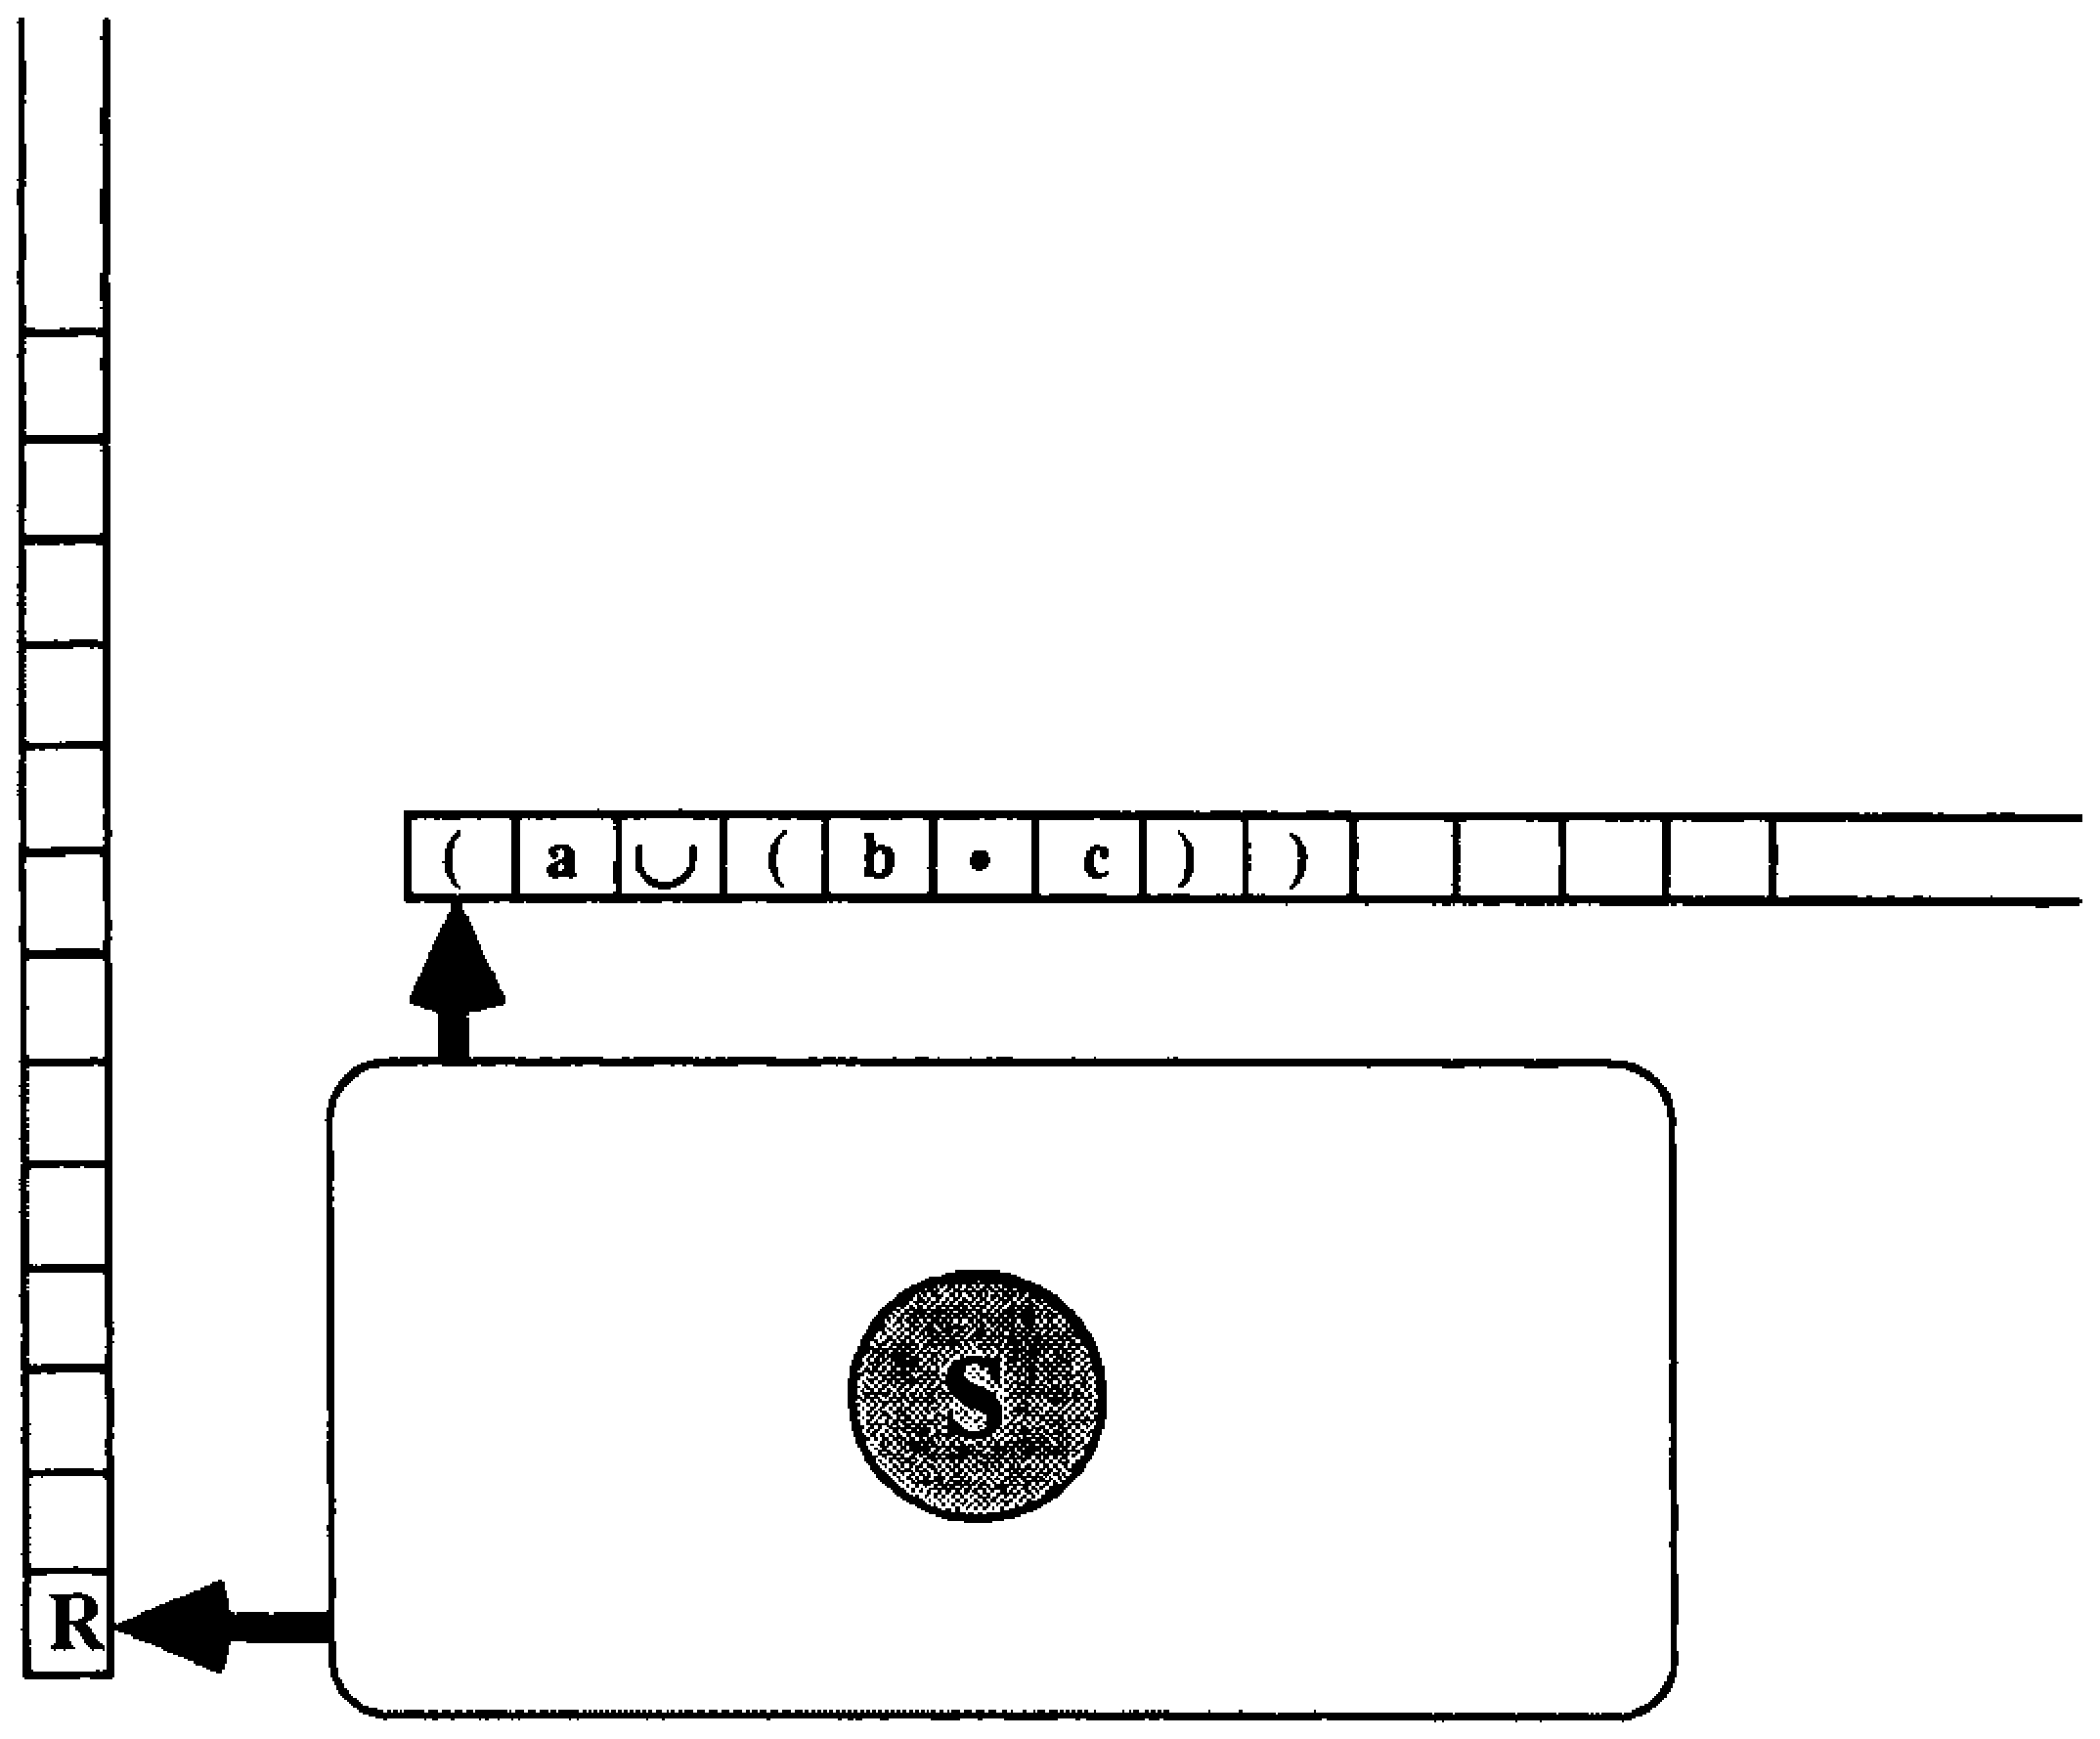
\epsfig{figure=ToFAfigures/fig10-5a.eps,height=2.0in}}
\caption{Walkthrough of the pushdown automaton discussed in Example 10.7}\label{fig-10.5a}
\end{figure}

% Figure 10.5b
\begin{figure}
\centerline{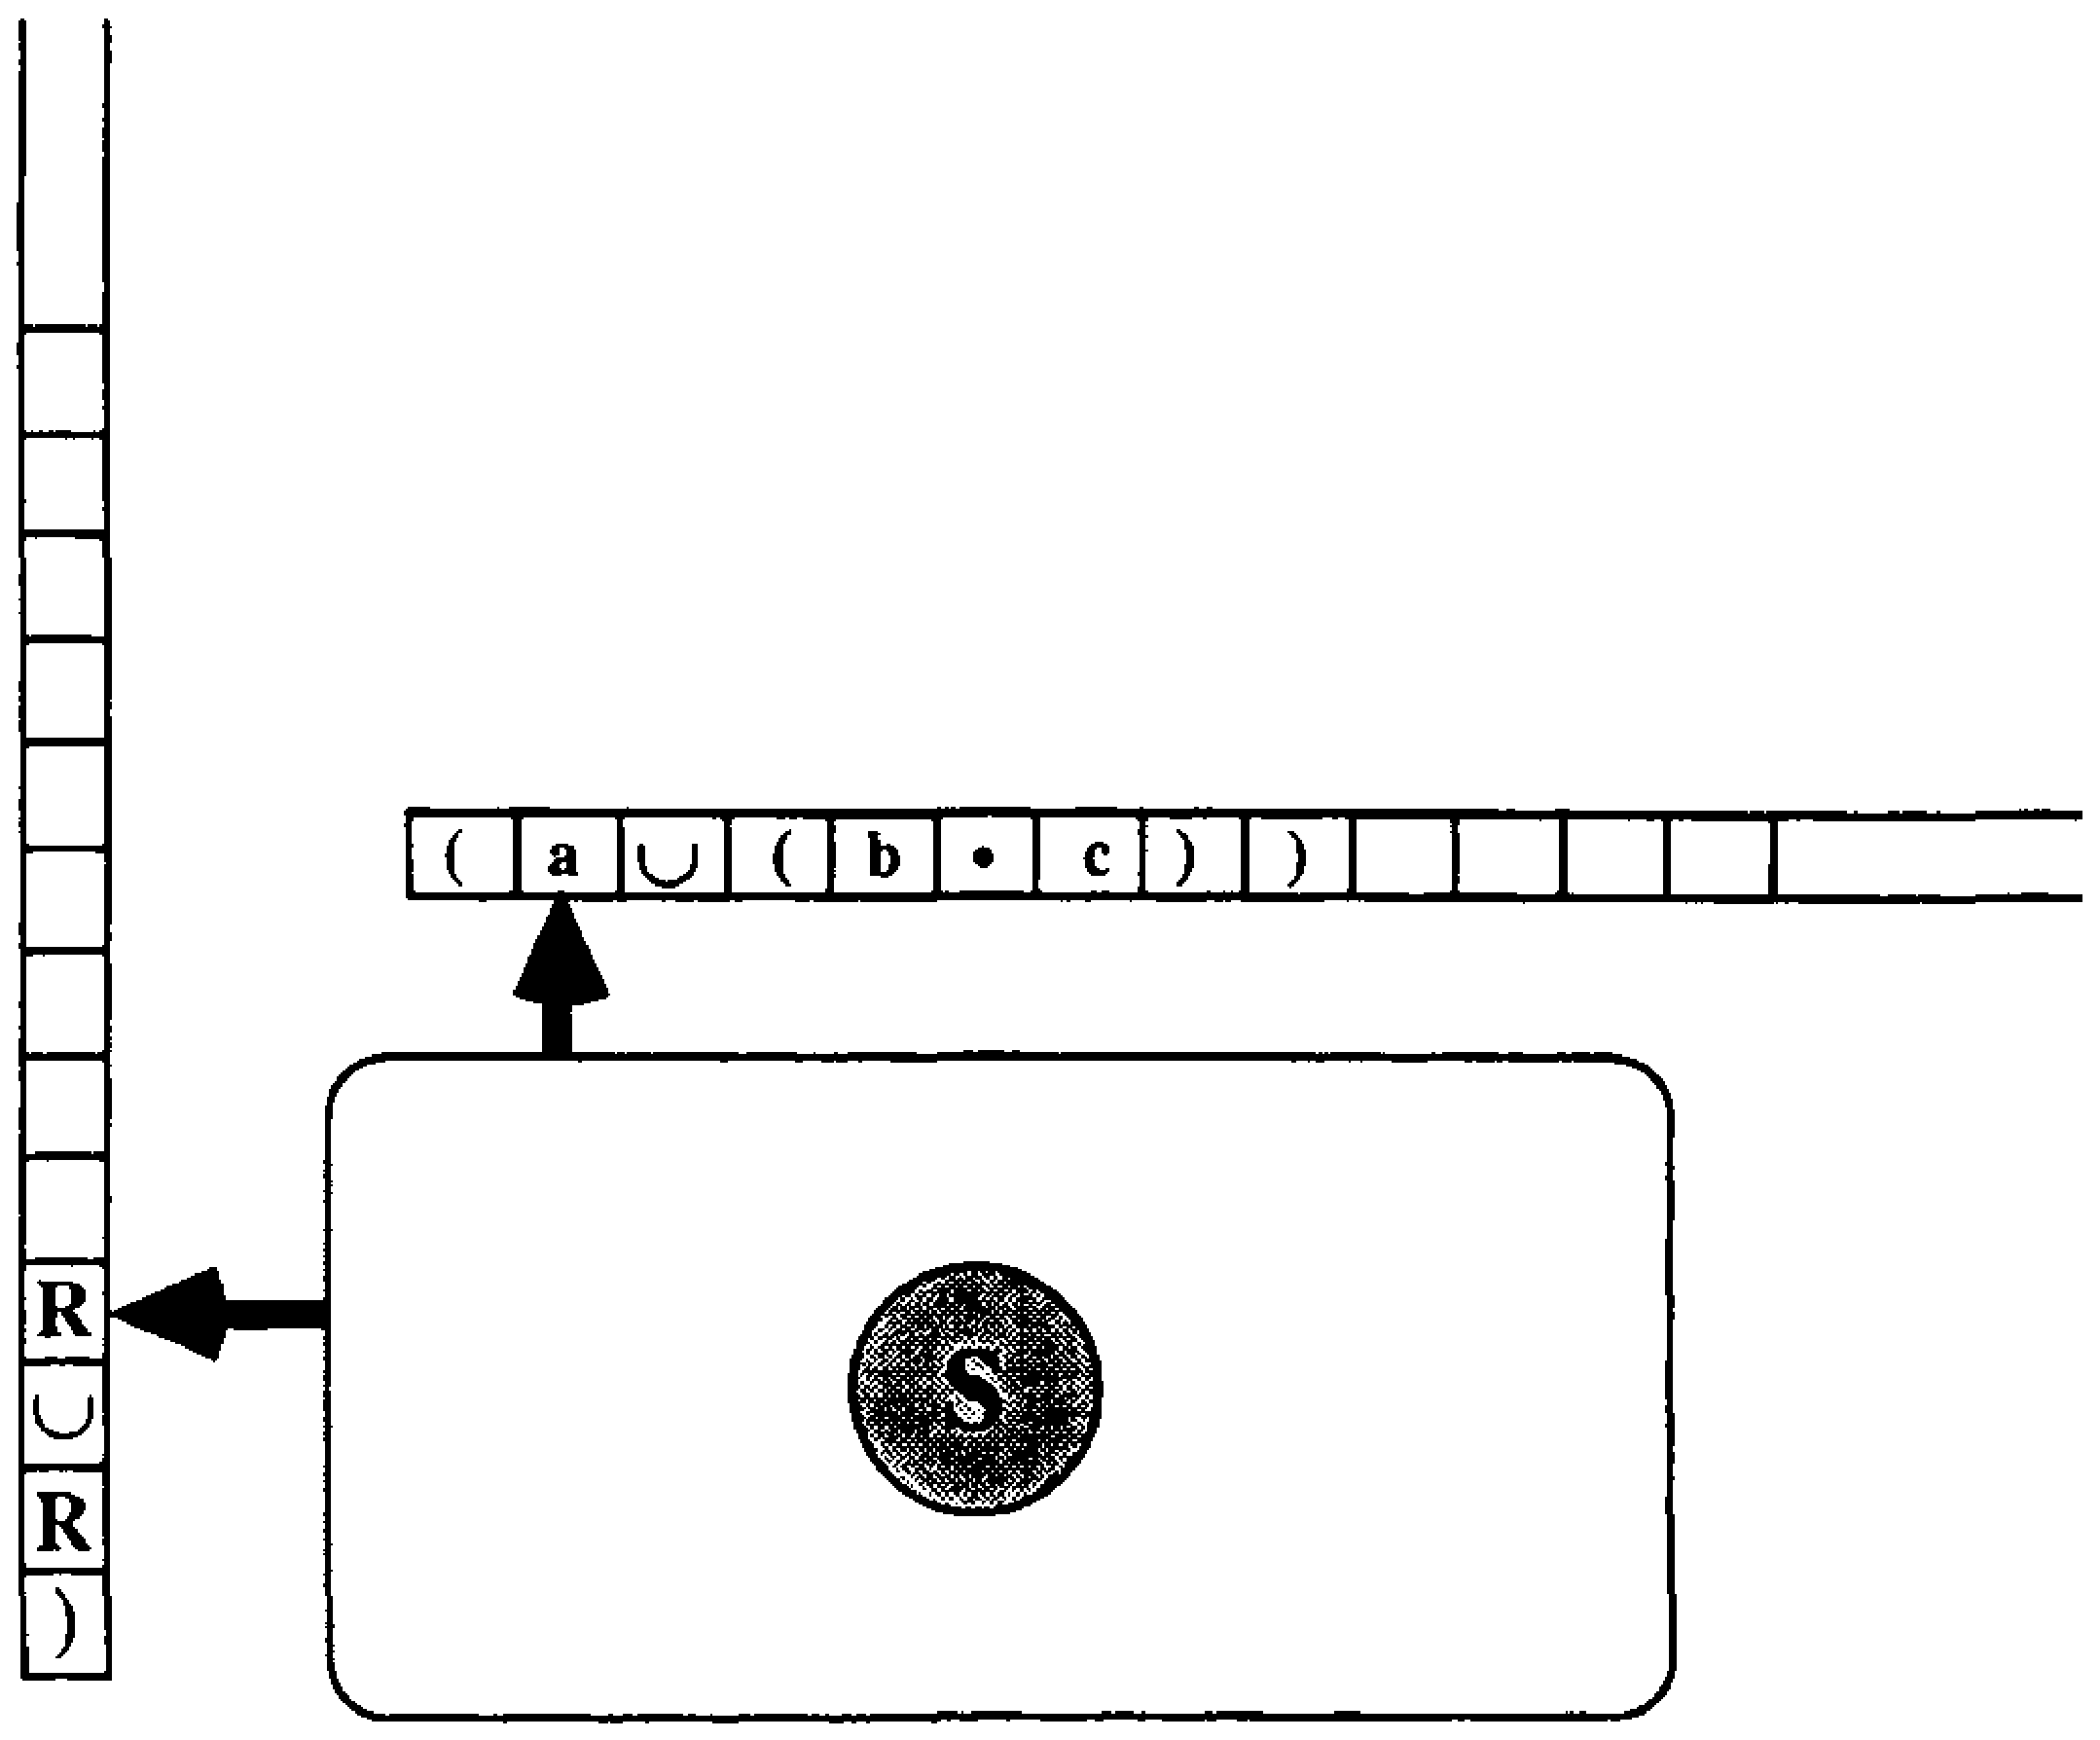
\epsfig{figure=ToFAfigures/fig10-5b.eps,height=2.0in}}
\caption{Walkthrough of the pushdown automaton discussed in Example 10.7}\label{fig-10.5b}
\end{figure}

% Figure 10.5c
\begin{figure}
\centerline{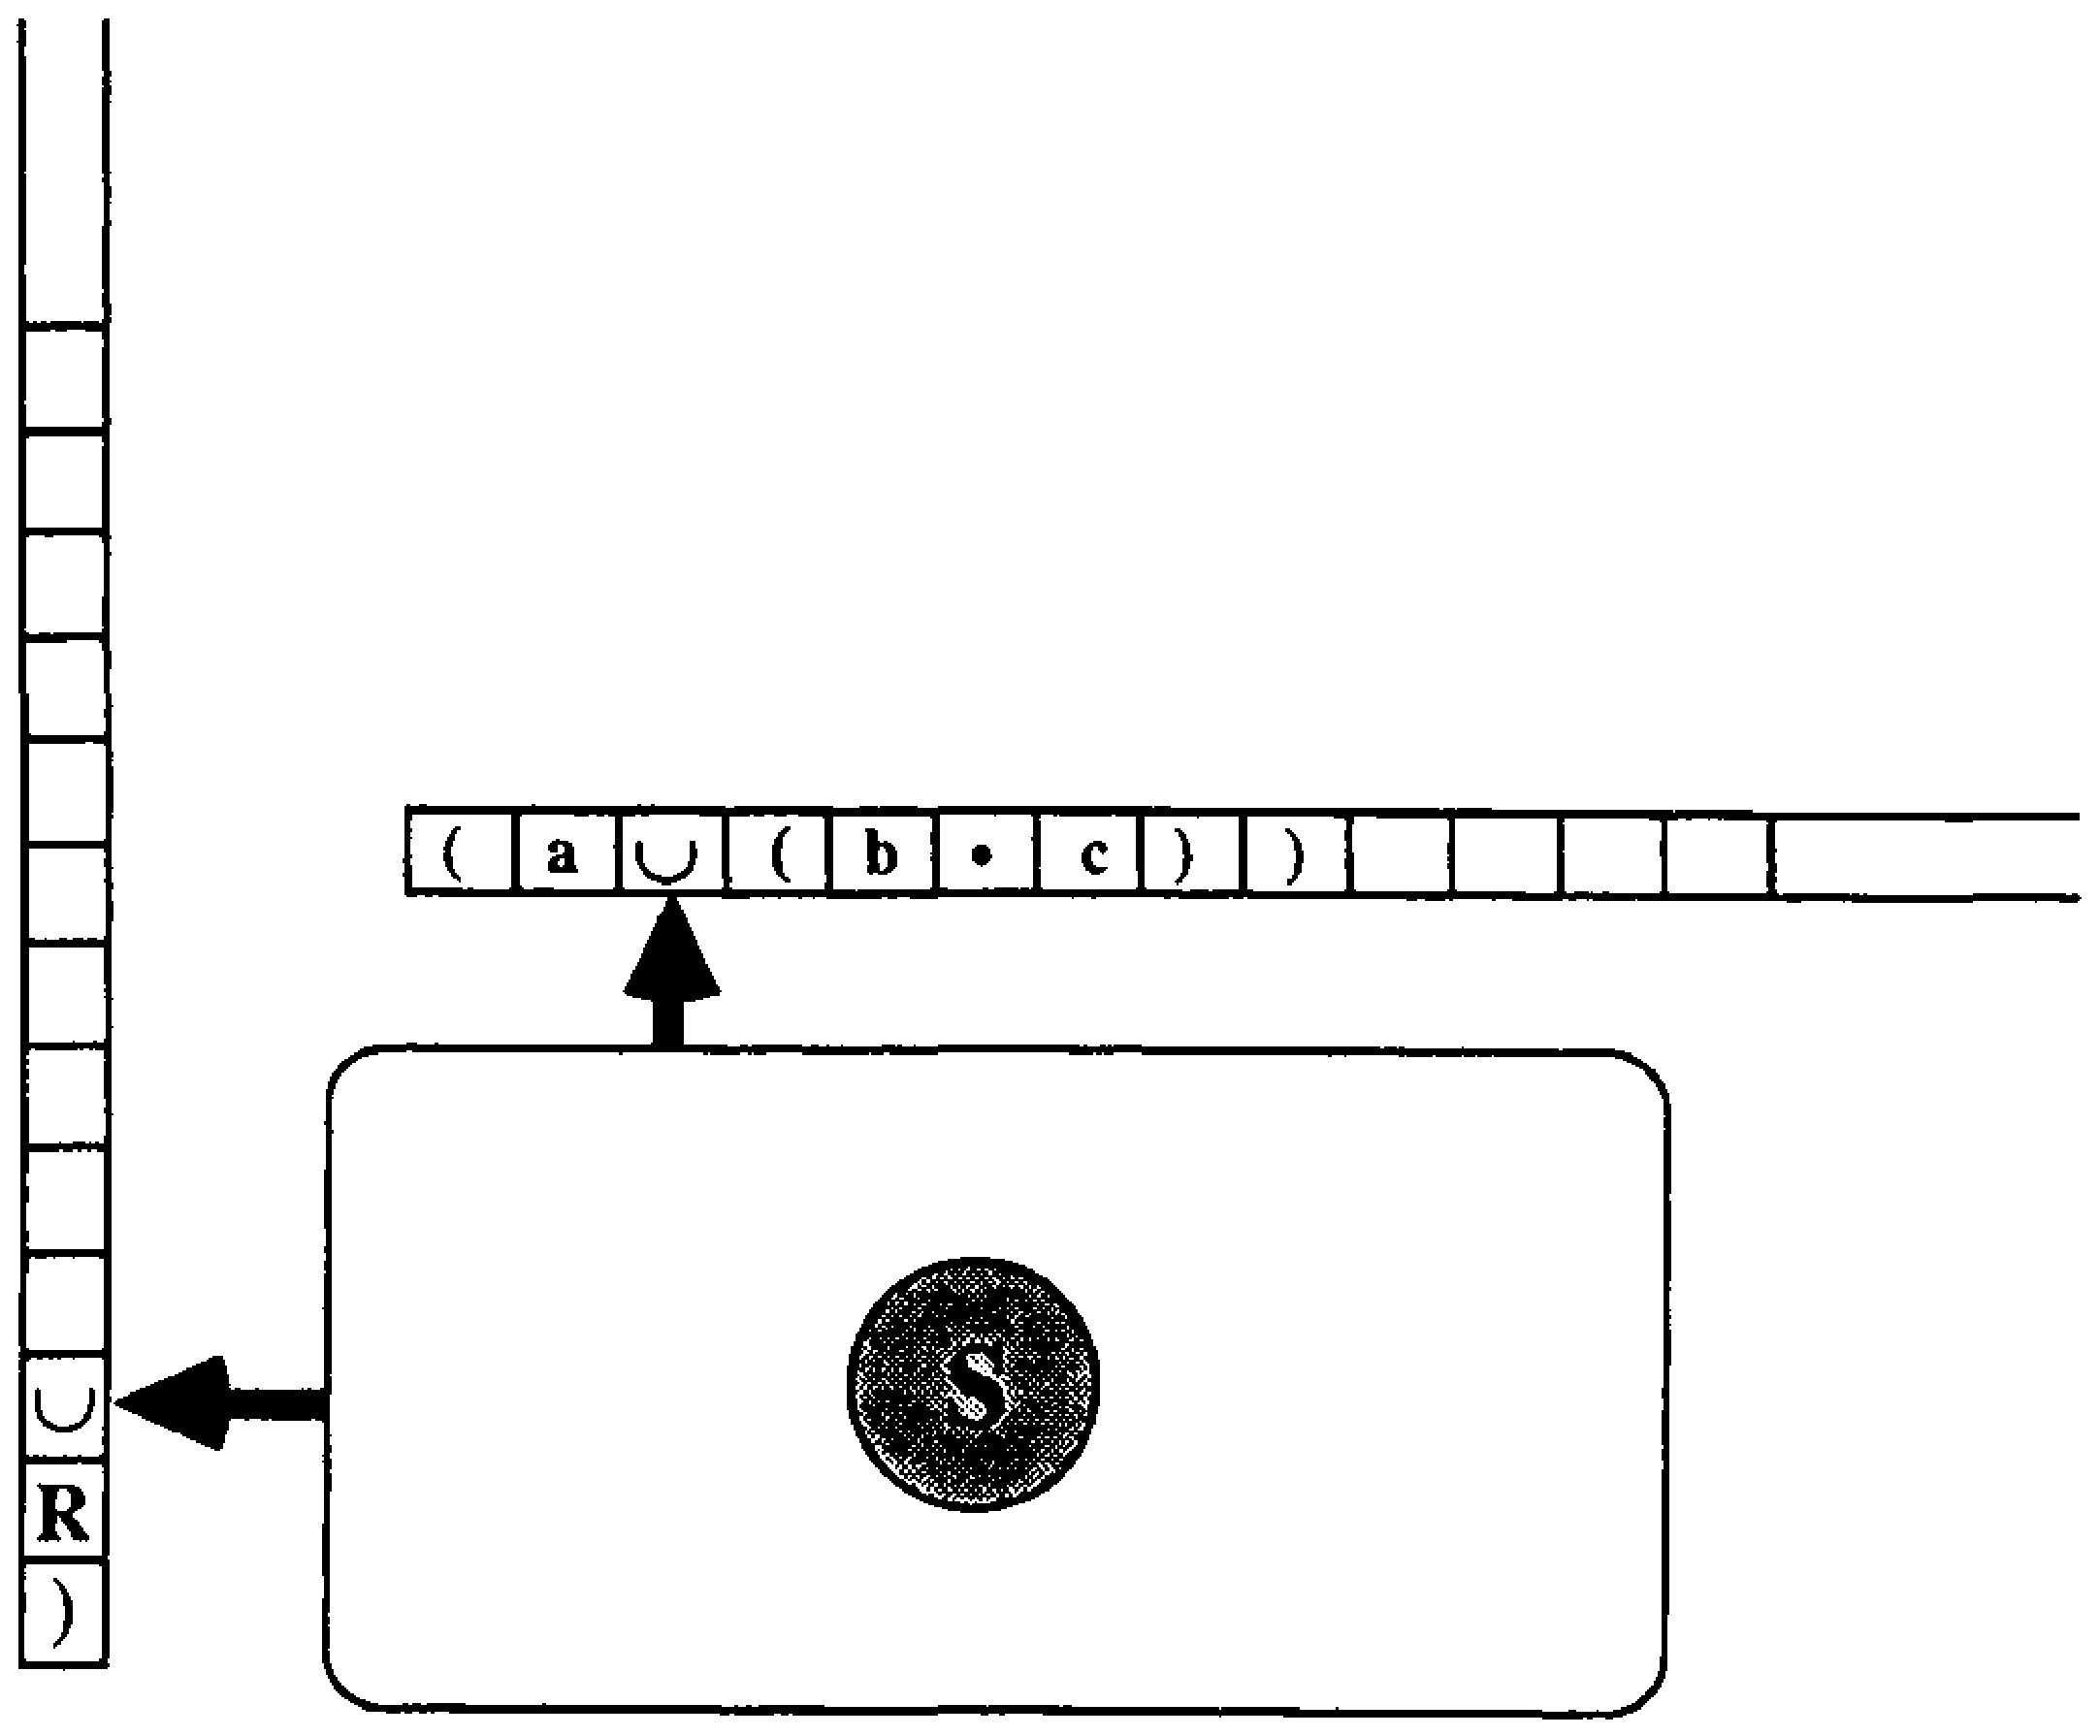
\epsfig{figure=ToFAfigures/fig10-5c.eps,height=2.0in}}
\caption{Walkthrough of the pushdown automaton discussed in Example 10.7}\label{fig-10.5c}
\end{figure}

% Figure 10.5d
\begin{figure}
\centerline{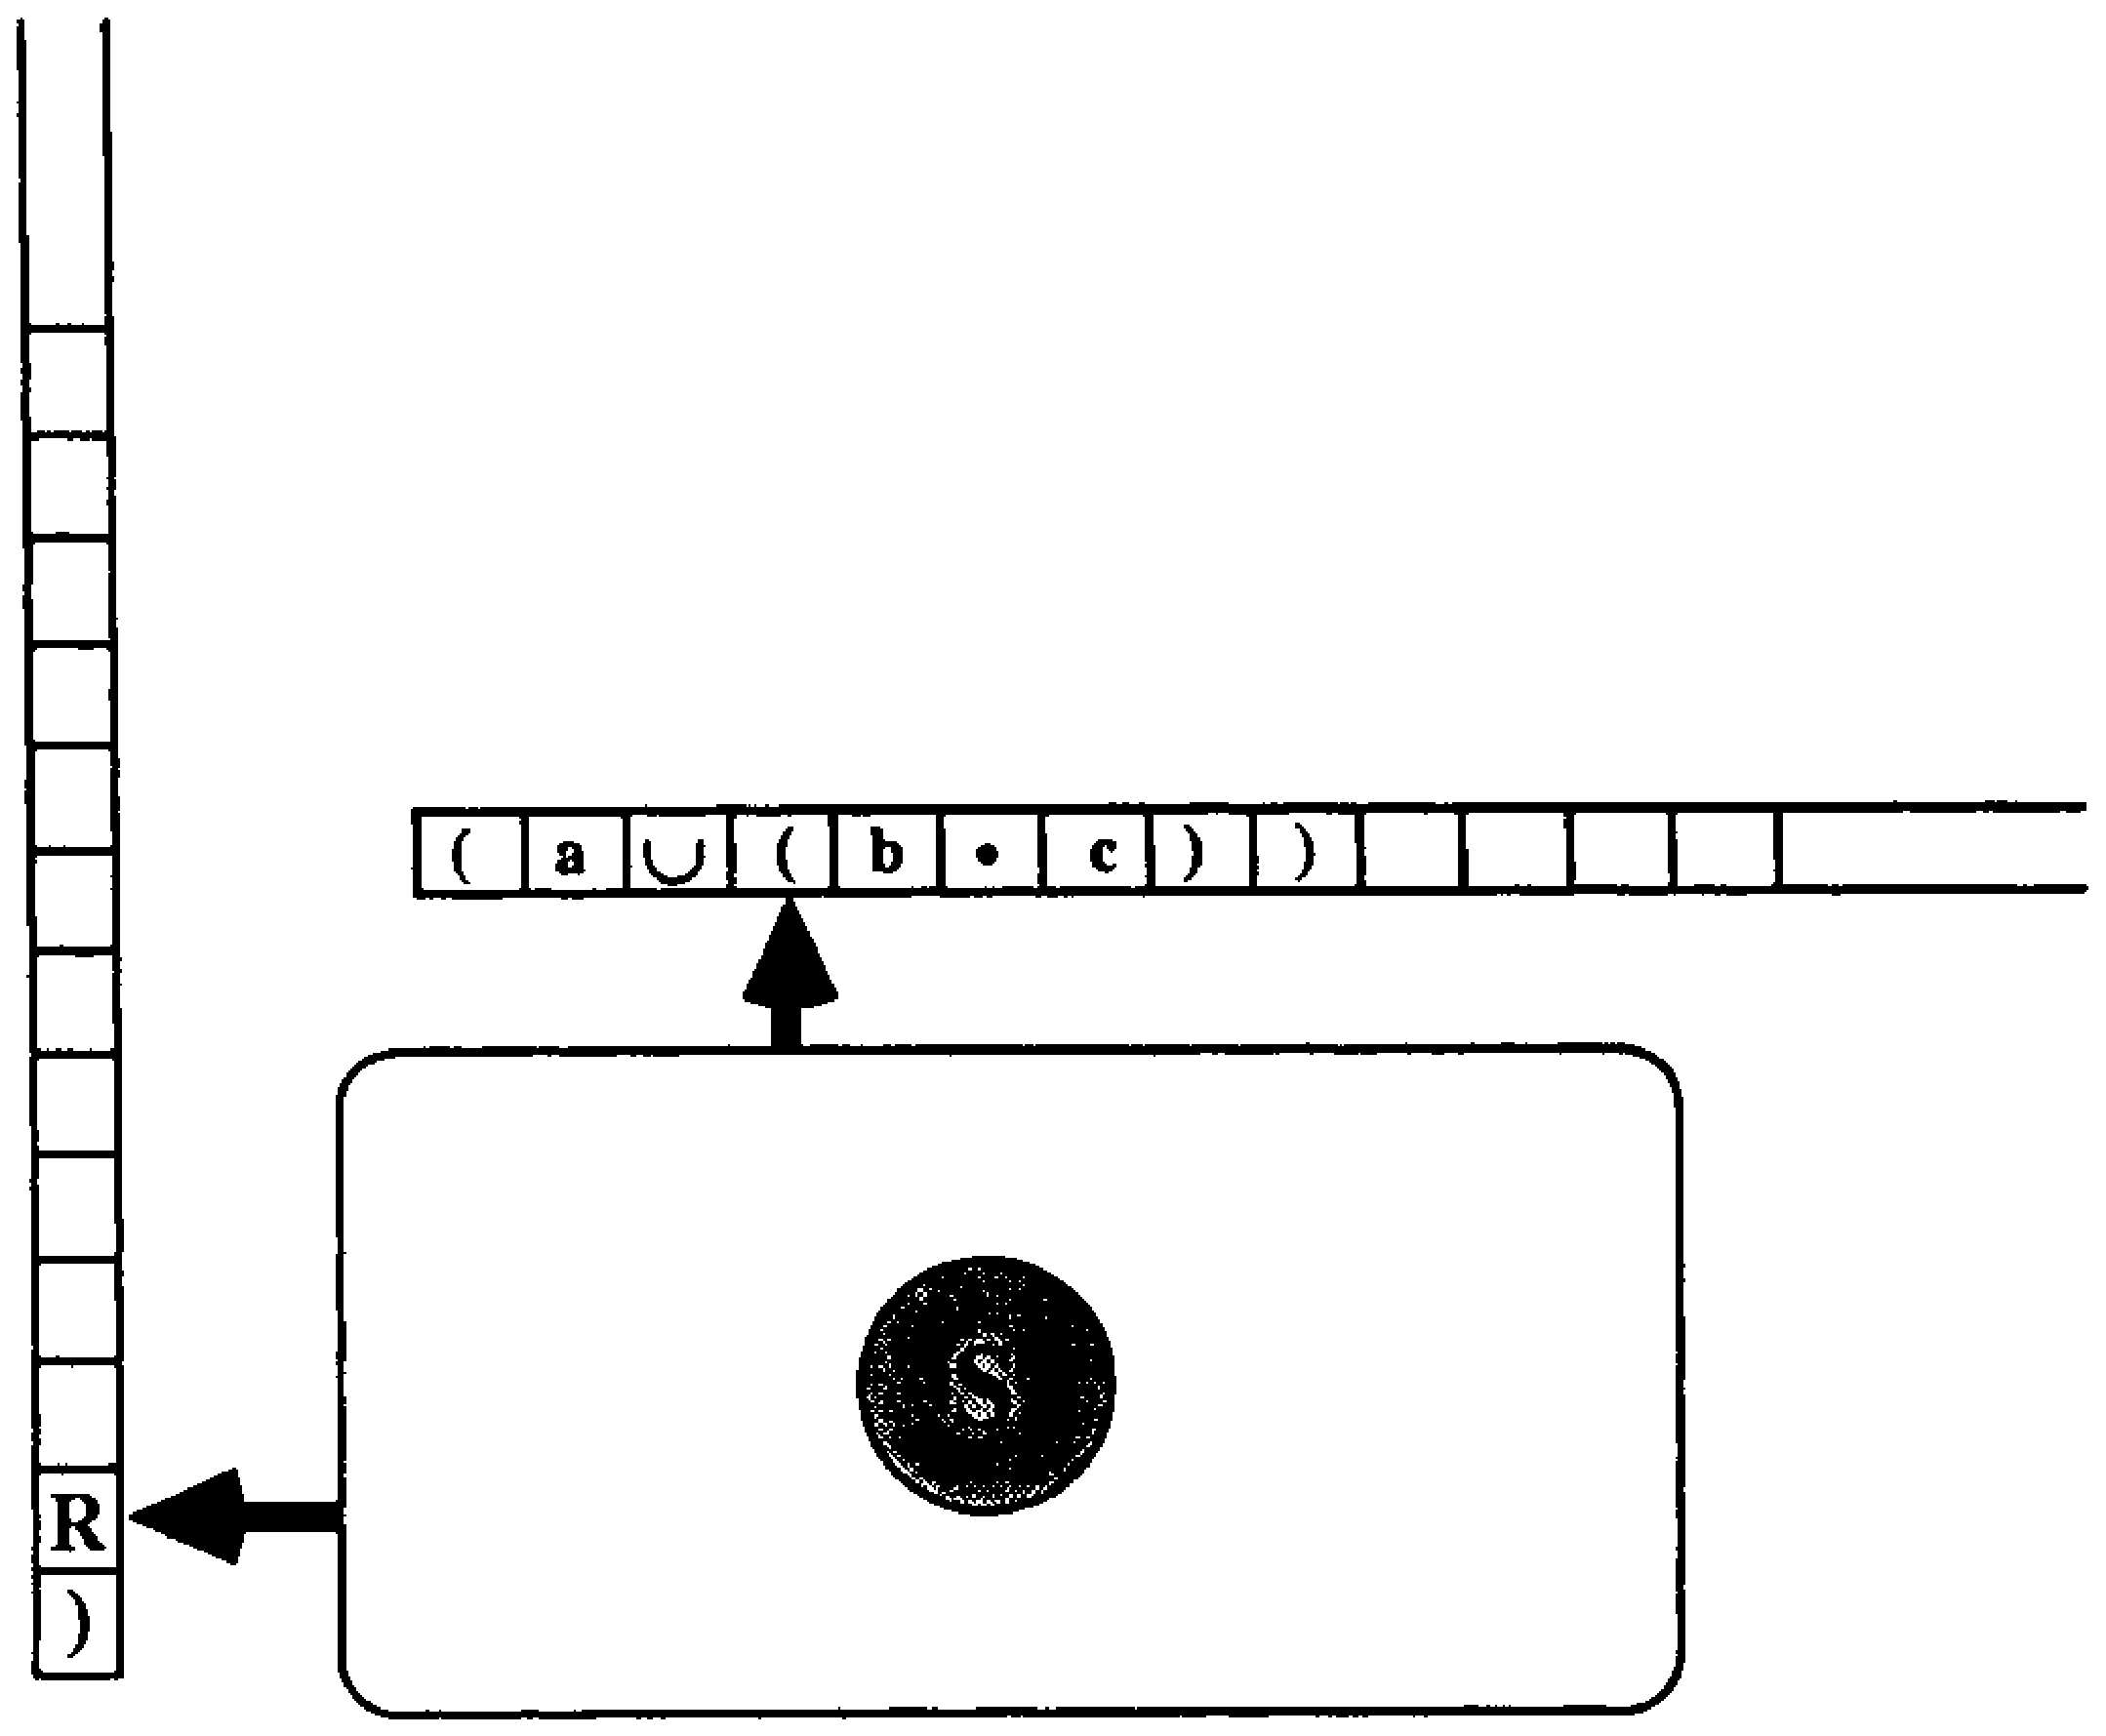
\epsfig{figure=ToFAfigures/fig10-5d.eps,height=2.0in}}
\caption{Walkthrough of the pushdown automaton discussed in Example 10.7}\label{fig-10.5d}
\end{figure}

% Figure 10.5e
\begin{figure}
\centerline{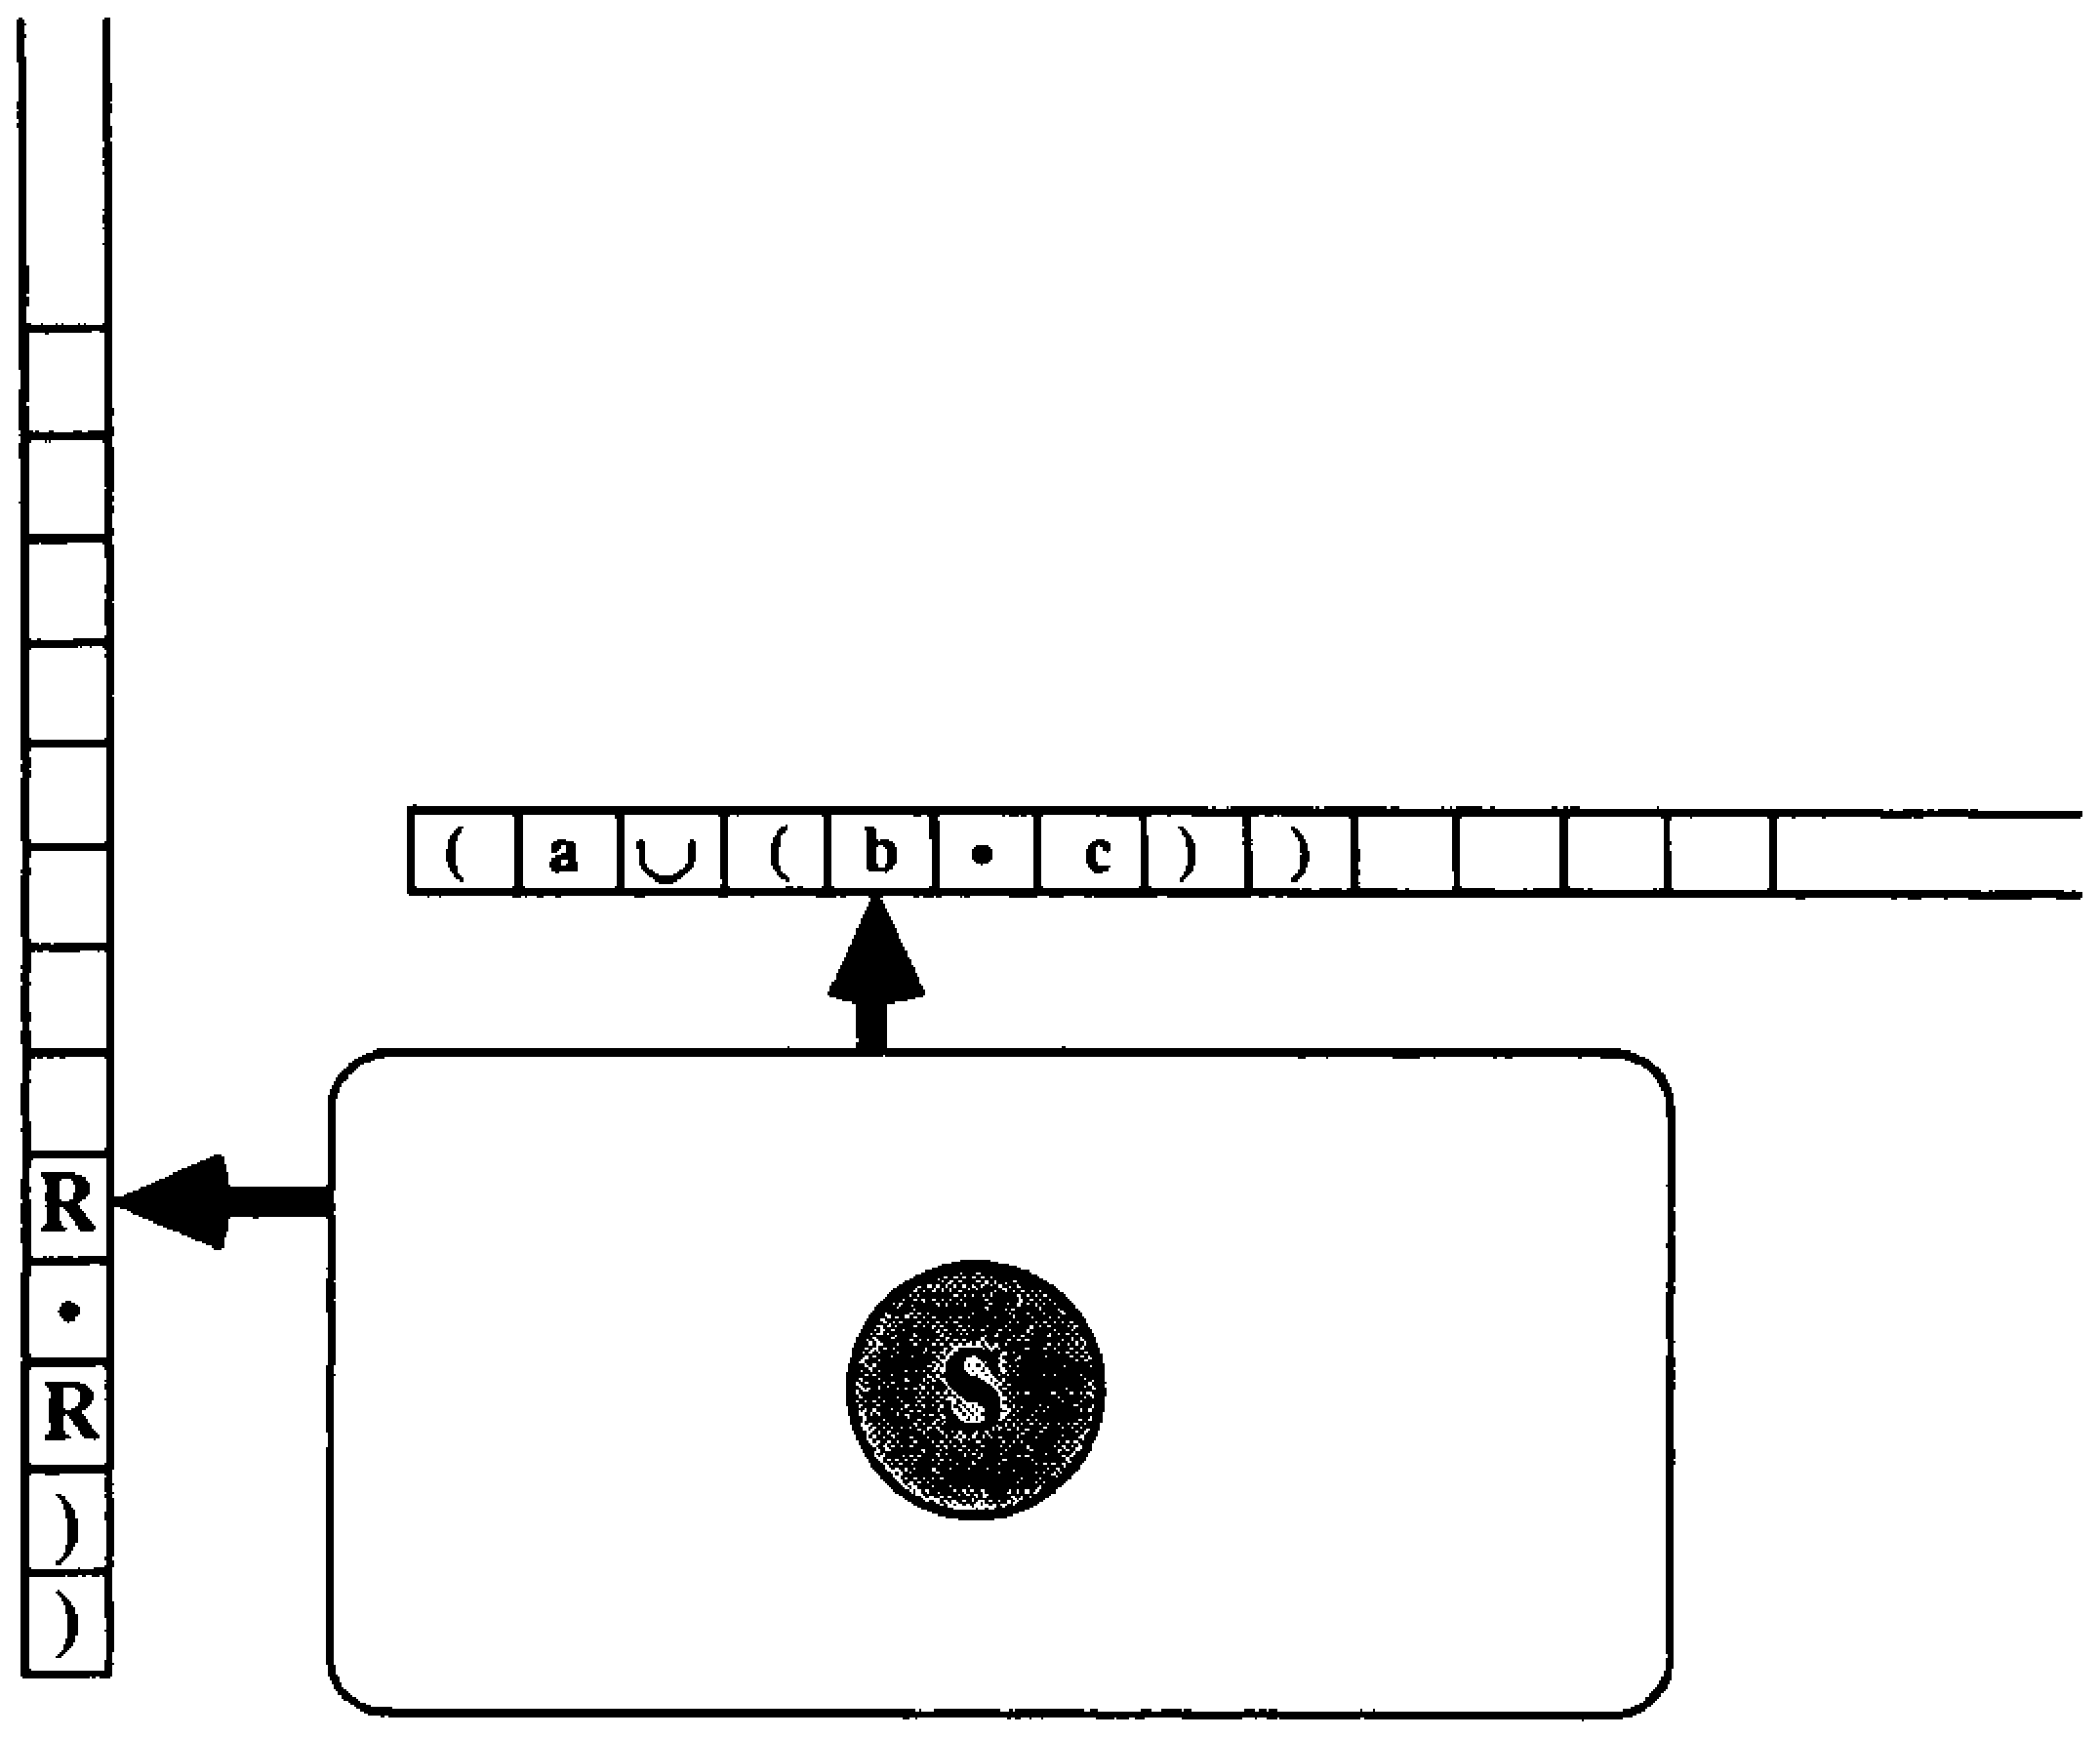
\epsfig{figure=ToFAfigures/fig10-5e.eps,height=2.0in}}
\caption{Walkthrough of the pushdown automaton discussed in Example 10.7}\label{fig-10.5e}
\end{figure}

% Figure 10.5f
\begin{figure}
\centerline{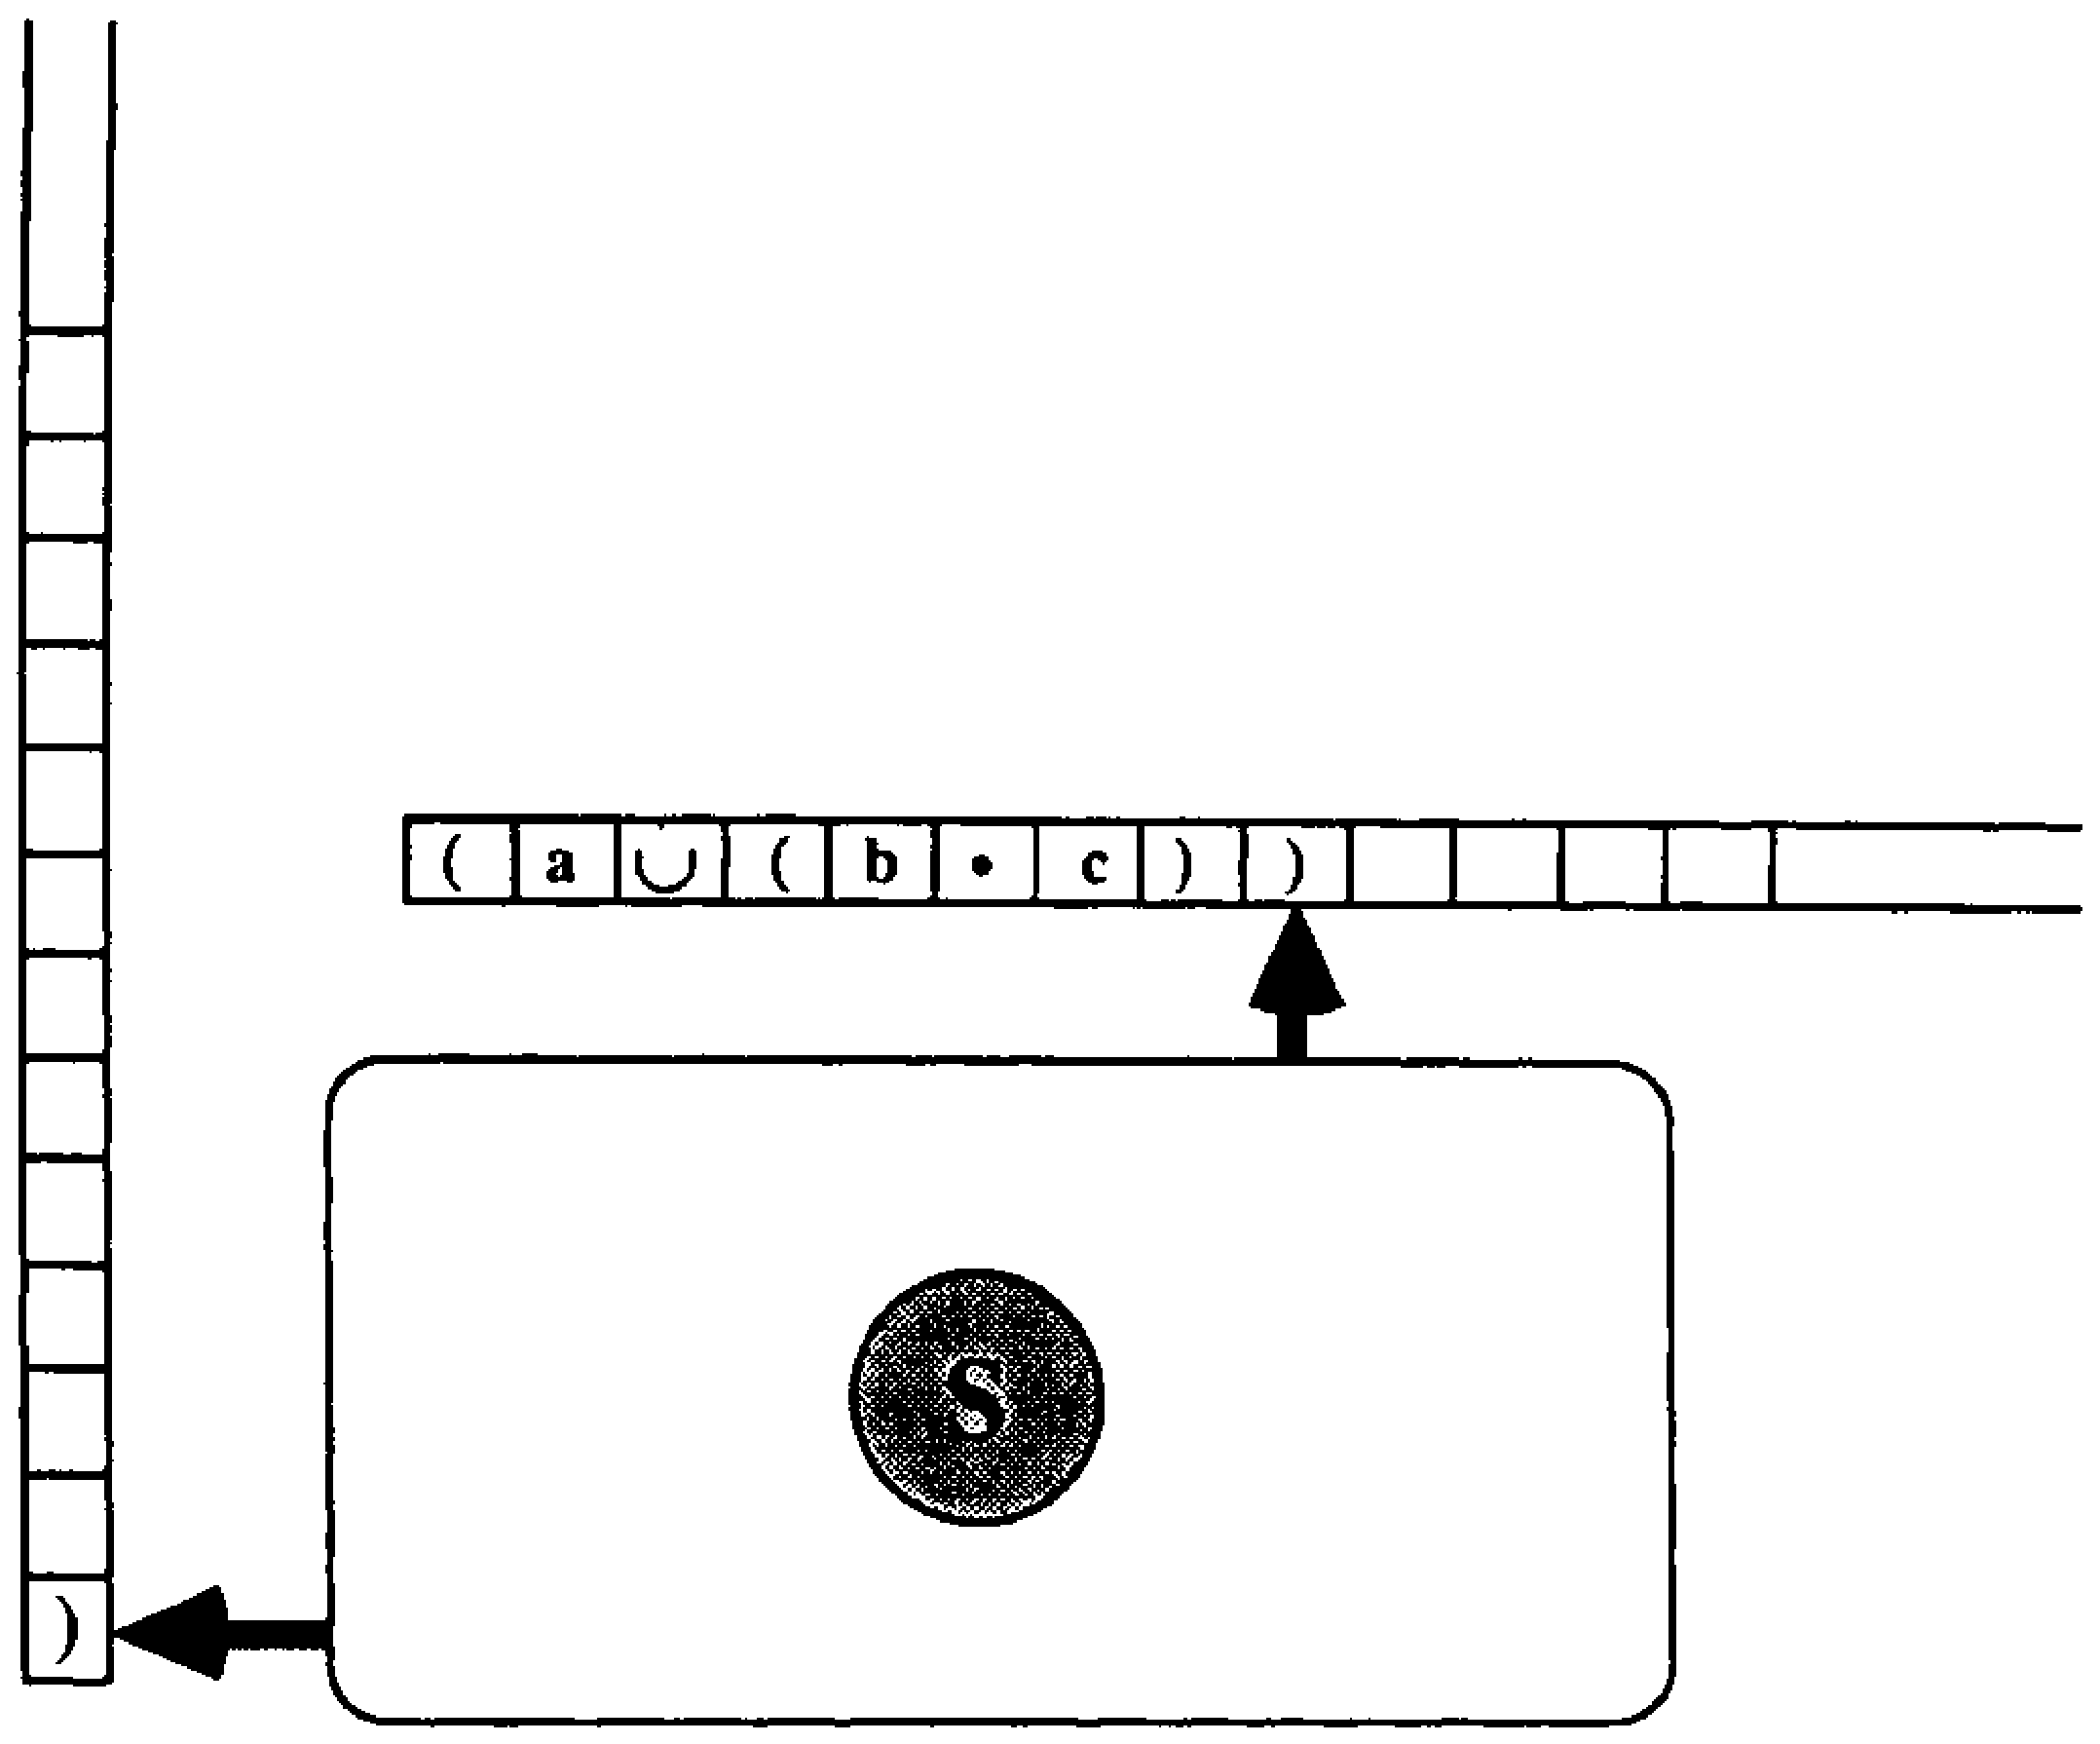
\epsfig{figure=ToFAfigures/fig10-5f.eps,height=2.0in}}
\caption{Walkthrough of the pushdown automaton discussed in Example 10.7}\label{fig-10.5f}
\end{figure}
\setcounter{figure}{5}                        %nasty kluge
\renewcommand{\thefigure}{\arabic{chapter}.\arabic{figure}}

% Theorem 10.2
\begin{thm}\label{thm-10.2}
Given any alphabet $\Sigma$, $\CSIG\subseteq\PSIG$. In particular, for any
context-free grammar $G$, there is a pushdown automaton that accepts (via empty
stack) the language generated by $G$.

\emph{Proof.} Let $G'$ be any context-free grammar. Theorem \ref{thm-9.6} guarantees that
there is a pure Greibach normal form grammar $G=\langle\Omega,\Sigma,S,P\rangle$
for which $L(G)=L(G')-\{\lambda\}$. If $\lambda\notin L(G')$, the PDA $P_G$ from
Definition \ref{dfn-10.6} can be used directly. If $\lambda\in L(G')$, then there is a
Greibach normal form grammar
\[ G''=\langle\Omega\cup\{Z\},\Sigma,Z,P\cup\{Z\rightarrow S,Z\rightarrow\lambda
	\}\rangle, \]
which generates $L(G')$, and the state transition function for $L(G')$ should
then include the move $\delta_G(s,\lambda,Z)=\{\langle s,S\rangle,\langle s,
\lambda\rangle\}$ to reflect the two $Z$-rules. The bottom of the stack symbol
would then be $Z$, the new start symbol.

In either case, induction on the number of moves in a sequence will show that\\
$(\forall x\in\Sigma^*)(\forall\beta\in(\Sigma\cup\Omega)^*)(\langle s,x,S
\rangle\Dvdash\langle s,\lambda,\beta\rangle  \ \ \  \Leftrightarrow\ \ \ S\ \DRightarrow x\beta$ as a
leftmost derivation).\\Note that $x\beta$ is likely to be a sentential form that
still contains nonterminals. The words $x$ that result in an empty stack ($\beta
=\lambda$) will then be exactly those words that produce an entire string of
terminal symbols from the start symbol $S$ (or $Z$ in the case where the grammar
contains the two special $Z$-rules). In other words, $L(G')=\Lambda(P_G)$.
\end{thm}

Given a context-free grammar, the definition of an equivalent PDA is easy once
an appropriate GNF grammar is in hand. In Example 10.6, the grammar was already
in Greibach normal form. To find a PDA for the grammar in Chapters \ref{ch-8} and \ref{ch-9} that
generates regular expressions, the grammar
\[ \langle\{R\},\{\pmb{a},\pmb{b},\pmb{c},\pmb{(},\pmb{)},\pmb{\epsilon},
	\pmb{\emptyset},\pmb{\cup},\pmb{\cdot},\pmb{^*}\},R,\{R\rightarrow
	\pmb{a}|\pmb{b}|\pmb{c}|\pmb{\epsilon}|\pmb{\emptyset}|\pmb{(}R
	\pmb{\cdot}R\pmb{)}|\pmb{(}R\pmb{\cup}R\pmb{)}|R\pmb{^*}\}\rangle \]
would have to be converted to Greibach normal form. The offending left-recursive
production $R\rightarrow R\pmb{^*}$ would have to be replaced, resulting in an
extra nonterminal and about three times as many productions. The definition of
the PDA for this grammar would be correspondingly more complex (see the
exercises).

Since every context-free language can be represented by a pushdown automaton
with only one state, one might suspect that more complex PDAs with extra states
may be able to define languages that are more complex than those in \CSIG. It
turns out that extra states yield no more cognitive power; the information
stored within the finite-state control can effectively be stored on the stack
tape. This will follow from the fact that the converse of Theorem \ref{thm-10.2}, that
context-free grammars have equivalent pushdown automata, is also true.

Defining a pushdown automaton based on a context-free grammar is not as elegant
as the construction presented in Definition \ref{dfn-10.6}, but the idea is to have the
leftmost derivations in the grammar correspond to successful move sequences in
the PDA.

% Definition 10.7
\begin{dfn}\label{dfn-10.7}
Let $P=\langle\Sigma,\Gamma,S,s_0,\delta,B,\emptyset\rangle$ be a pushdown
automaton. Define the grammar $G_P=\langle\Omega,\Sigma,Z,P_P\rangle$, where
\[ \Omega=\{Z\}\cup\{A^{st}|\ A\in\Gamma,s,t\in S\} \]
and
\begin{center}\begin{tabular}{r@{ }c@{ }l}
$P_P$ & $=$ & $\{Z\rightarrow B^{s_0t}|\ t\in S\}\cup\{A^{sq}\rightarrow\pmb{a}A^{rt_1}_1
	A^{t_1t_2}_2A^{t_2t_3}_3\cdots A^{t_{m-1}t_m}_{m-1}A^{t_mq}_m|\ A\in\Gamma,
	\pmb{a}\in\Sigma\cup\{\lambda\},$ \\
&& $\langle r,A_1A_2\cdots A_m\rangle\in\delta(s,\pmb{a},A),s,q,r,t_1,t_2,\ldots,
	t_m\in S\}$ \\
&& $\cup\ \{A^{sr}\rightarrow\pmb{a}\ |\ s,r\in S,A\in\Gamma,\pmb{a}\in\Sigma\cup\{
	\lambda\},\langle r,\lambda\rangle\in\delta(s,\pmb{a},A)\}$
\end{tabular}\end{center}
\end{dfn}

Note that when $m=1$, the transition $\langle r,A_1\rangle\in\delta(s,\pmb{a},A)$
gives rise to a rule of the form $A^{sq}\rightarrow\pmb{a}A^{rq}_1$ for each
state $q\in S$.

\subsection*{Example 10.8}

Consider again the pushdown automaton from Example 10.4, defined by $P_2=\langle
\{\pmb{a},\pmb{b}\},\{S,C\},\{t\},t,\delta,S,\emptyset\rangle$, where $\delta$
is given by
\begin{center}\begin{tabular}{r@{ = }l}
$\delta(t,\pmb{a},S)$ & $\{\langle t,SC\rangle,\langle t,C\rangle\}$ \\
$\delta(t,\pmb{a},C)$ & $\{\ \ \}$ \\
$\delta(t,\pmb{b},S)$ & $\{\ \ \}$ \\
$\delta(t,\pmb{b},C)$ & $\{\langle t,\lambda\rangle\}$
\end{tabular}\end{center}
Since there is but one state and two stack symbols, the nonterminals for the
corresponding grammar $G_{P_2}$ are $\Omega=\{Z,S^{tt},C^{tt}\}$. $P_{P_2}$ can
be calculated as follows: $Z\rightarrow S^{tt}$ is the only rule arising from
the first criteria for productions. Since $\delta(t,\pmb{a},S)$ contains
$\langle t,SC\rangle$, a move that produces two stack symbols, $m=2$ and the
resulting production is $S^{tt}\rightarrow\pmb{a}S^{tt}C^{tt}$. The only other
rule due to the second criteria arises because $\delta(t,\pmb{a},S)$ contains
$\langle t,C\rangle$, which with $m=1$ yields $S^{tt}\rightarrow\pmb{a}C^{tt}$.
Finally, $\langle t,\lambda\rangle\in\delta(t,\pmb{b},C)$ causes $C^{tt}
\rightarrow\pmb{b}$ to be added to the production set. The resulting grammar is
therefore
\[ G_{P_2}=\langle\{Z,S^{tt},C^{tt}\},\{\pmb{a},\pmb{b}\},Z,\{Z\rightarrow
	S^{tt},S^{tt}\rightarrow\pmb{a}S^{tt}C^{tt},S^{tt}\rightarrow\pmb{a}
	C^{tt},C^{tt}\rightarrow\pmb{b}\}\rangle \]
and $G_{P_2}$ does indeed generate $\{\pmb{a}^n\pmb{b}^n|\ n \geq 1\}$ and is
therefore equivalent to $P_2$.

\subsection*{Example 10.9}

Now consider the pushdown automaton from Example 10.1, defined by
\[ P_1 = \langle\{\pmb{a},\pmb{b}\},\{A,B\},\{q,r\},q,\delta,B,\emptyset\rangle, \]
where the nonempty transitions were
\begin{center}\begin{tabular}{r@{ = }l}
$\delta(q,\pmb{a},B)$ & $\{\langle q,A\rangle\}$ \\
$\delta(q,\pmb{a},A)$ & $\{\langle q,AA\rangle\}$ \\
$\delta(q,\pmb{b},A)$ & $\{\langle r,\lambda\rangle\}$ \\
$\delta(r,\pmb{b},A)$ & $\{\langle r,\lambda\rangle\}$
\end{tabular}\end{center}
Since there are two stack symbols and two choices for each of the state
superscripts, the nonterminal set for the grammar $G_{P_1}$ is $\Gamma=\{Z,B^{qq},
B^{qr},B^{rq},B^{rr},A^{qq},A^{qr},A^{rq},A^{rr}\}$, although some of these will
turn out to be useless.

$P_{P_1}$ contains the $Z$-rules $Z\rightarrow B^{qq}$ and $Z\rightarrow B^{qr}$
from the first criteria for productions. The transition $\delta(q,\pmb{a},B) =
\{\langle q,A\rangle\}$ accounts for the productions $B^{qr}\rightarrow\pmb{a}
A^{qr}$ and $B^{qq}\rightarrow\pmb{a}A^{qq}$\!. $\delta(q,\pmb{a},A)=\{\langle q,
AA\rangle\}$ gives rise to the $A^{qq}$\!-rules $A^{qq}\rightarrow\pmb{a}A^{qq}\!\!
A^{qq}$ and $A^{qq}\rightarrow\pmb{a}A^{qr}\!\!\!A^{rq}$, as well as $A^{qr}$\!-rules
$A^{qr}\rightarrow\pmb{a}A^{qq}\!\!A^{qr}$ and $A^{qr}\rightarrow\pmb{a}A^{qr}\!\!A^{rr}$\!\!.
$\delta(q,\pmb{b},A)=\{\langle r,\lambda\rangle\}$ accounts for another
$A^{qr}$-rule, $A^{qr}\rightarrow\pmb{b}$. Finally, the transition $\delta(r,
\pmb{b},A)=\{\langle r,\lambda\rangle\}$ generates the only $A^{rr}$\!-rule,
$A^{rr}\rightarrow\pmb{b}$.

Note that some of the potential nonterminals ($B^{qr}\!,B^{rq}\!,B^{rr}$) are never
generated, and others ($A^{qq}\!,B^{qq}$) cannot produce terminal strings. The
resulting grammar, with useless items deleted, is given by
\[ G_{P_1}=\langle\{Z,B^{qr}\!\!,A^{qr}\!\!,A^{rr}\},\{\pmb{a},\pmb{b}\},Z,\{Z
	\rightarrow B^{qr}\!\!,B^{qr}\rightarrow\pmb{a}A^{qr}\!\!,A^{qr}\rightarrow
	\pmb{a}A^{qr}\!\!A^{rr}\!\!,A^{qr}\rightarrow\pmb{b},A^{rr}\rightarrow\pmb{b}\}
	\rangle \]
and $G_{P_1}$ generates the language $P_1$ recognizes: $\{\pmb{a}^n\pmb{b}^n|\ n
\geq 1\}$.

Notice that the move sequence
\begin{center}\begin{tabular}{r@{ $\vdash$ }l}
$\langle q,\pmb{aaabbb},B\rangle$ & $\langle q,\pmb{aabbb},A\rangle$ \\
& $\langle q,\pmb{abbb},AA\rangle$ \\
& $\langle q,\pmb{bbb},AAA\rangle$ \\
& $\langle r,\pmb{bb},AA\rangle$ \\
& $\langle r,\pmb{b},A\rangle$ \\
& $\langle r,\lambda,\lambda\rangle$
\end{tabular}\end{center}
corresponds to the leftmost derivation
\begin{center}\begin{tabular}{r@{ $\Rightarrow$ }l}
$Z\Rightarrow B^{qr}$ & $\pmb{a}A^{qr}$ \\
& $\pmb{aa}A^{qr}\!\!A^{rr}$ \\
& $\pmb{aaa}A^{qr}\!\!A^{rr}\!\!A^{rr}$ \\
& $\pmb{aaab}A^{rr}\!\!A^{rr}$ \\
& $\pmb{aaabb}A^{rr}$ \\
& $\pmb{aaabbb}$
\end{tabular}\end{center}

Note the relationship between the sequence of stack configurations and the
nonterminals in the corresponding sentential form. For example, when $\pmb{aaa}$
has been processed by $P_1$, $AAA$ is on the stack, and when the leftmost
derivation has produced $\pmb{aaa}$, the remaining nonterminals are also three
$A$-based symbols ($A^{qr}\!\!A^{rr}\!\!A^{rr}$). $A^{qr}$ denotes a nonterminal (which
corresponds to the stack symbol $A$) that will eventually produce a terminal
string as the stack shrinks below the current size during a sequence of
transitions that lead from state $q$ to state $r$. This finally happens in the
last of the following steps, where $\pmb{aaa}A^{qr}\!\!A^{rr}\!\!A^{rr}\ \DRightarrow
\pmb{aaabbb}$. $A^{rr}$\!, by contrast, denotes a nonterminal (again corresponding
to the stack symbol $A$) that will produce a terminal string as the stack
shrinks in size during transitions from state $r$ back to state $r$. In this
example, this occurs in the next to the last two steps. The initial stack symbol
position held by $B$ is finally vacated during a sequence of transitions from
$q$ to $r$, and hence $B^{qr}$ appears in the leftmost derivation. On the other
hand, it was not possible to vacate $B$'s position during a sequence of moves
from $q$ to $q$, so $B^{qq}$ consequently does not participate in significant
derivations.

The strong correspondence between profitable move sequences in $P$ and valid
leftmost derivations in $G_P$ forms the cornerstone of the following proof.

% Theorem 10.3
\begin{thm}\label{thm-10.3}
Given any alphabet $\Sigma$, $\PSIG\subseteq\CSIG$. In particular, for any
pushdown automaton $P$, there is a context-free grammar $G_P$ for which $L(G_P)
= \Lambda(P)$.

\emph{Proof.} Let $P=\langle\Sigma,\Gamma,S,s_0,\delta,B,\emptyset\rangle$ be a
pushdown automaton, and let $G_P$ be the grammar given in Definition \ref{dfn-10.7}. The
key to the proof is to show that all words accepted by empty stack in the PDA
$P$ can be generated by $G_P$ and that only such words can be generated by $G_P$.
That is, we wish to show that the automaton halts in some state $t$ with an
empty stack after processing the terminal string $x$ exactly when there is a
leftmost derivation of the form
\[ Z \Rightarrow A^{s_0t}\  \DRightarrow x \]
That is,
\[ (\forall x\in\Sigma^*)(Z\Rightarrow B^{s_0t}\ \DRightarrow x  \ \ \  \Leftrightarrow\ \ \  
	\langle s_0,x, B\rangle \Dvdash \langle t,\lambda,\lambda\rangle) \]
The desired conclusion, that $L(G_P) = \Lambda(P)$, will follow immediately from
this equivalence. The equivalence does not easily lend itself to proof by
induction on the length of $x$; indeed, to progress from the $m^{th}$ to the
$m+1^{st}$ step, a more general statement involving more of the nonterminals of
$G_P$ is needed. The following statement can be proved by induction on the
number of moves and leads to the desired conclusion when $s=s_0$ and $A=B$:
\[ (\forall x\in\Sigma^*)(\forall A\in\Gamma)(\forall s\in S)(\forall t\in S)
	(A^{st}\ \DRightarrow x \ \ \  \Leftrightarrow\ \ \  \langle s,x,A\rangle \Dvdash
	\langle t,\lambda,\lambda\rangle) \]
The resulting grammar will then generate $\Lambda(P)$, but $G_P$ may not be a
strict context-free grammar; $\lambda$-moves may result in some productions of
the form $A^{sr}\rightarrow\lambda$, which will then have to be ``removed,'' as
specified by Exercise 9.16.
\end{thm}

Thus, $\PSIG=\CSIG$. Furthermore, only one state in a PDA is truly necessary, as
noted in the following corollary. In essence, this means that for PDAs that
accept by empty stack, any state information can be effectively encoded with the
information on the stack.

% Corollary 10.1
\begin{cor}\label{cor-10.1}
For every PDA $P$ that accepts via empty stack, there is an equivalent one-state
PDA $P'$ that also accepts via empty stack.

\emph{Proof.} Let $P$ be a PDA that accepts via empty stack. Let $P'=P_{G_P}$.
That is, from the original PDA $P$, find the corresponding context-free grammar
$G_P$. By Theorem \ref{thm-10.3}, this is equivalent to $P$. However, by Theorem \ref{thm-10.2}, the
grammar $G_P$ has an equivalent one-state PDA, which must also be equivalent to
$P$.
\end{cor}

Unlike the pushdown automata discussed in this section, PDAs that accept via
final state cannot always make do with a single state. As the exercises will
make clear, at least one final and one nonfinal state are typically necessary. Unlike
DFAs, PDAs with only one state \emph{can} accept some nontrivial languages, since
selected words can be rejected because there is no appropriate move sequence.
However, a single final state and a single nonfinal state
\emph{are} sufficient for full generality, as
shown in the following section.

\section{Equivalence Of Acceptance By Final State and Empty Stack}\label{sec-10.3}

In this section, we explore the ramifications of accepting words according to
the criteria that a final state can be reached after processing all the letters
on the input tape, rather than the criteria that the stack is emptied. Theorem
\ref{thm-10.4} will show that any language that can be accepted via empty stack can also
be accepted via final state. In terms of Definition \ref{dfn-10.5}, this means that
$\PSIG\subseteq\FSIG$. Since $\PSIG=\CSIG$, this means that every context-free
language can be accepted by a PDA via final state. Theorem \ref{thm-10.5} ensures that no
``new'' languages can be produced by pushdown automata that accept via final
state; $\FSIG\subseteq\PSIG$, and so $\FSIG=\PSIG=\CSIG$.

As in the last section, the key to the correspondence is the definition of an
appropriate translation from one finite representation to another. We first
consider a scheme for modifying a PDA so that the new device can transfer to a
final state whenever the old device was capable of emptying its stack. To do
this, we need to place a ``buffer'' symbol at the bottom of the stack, which will
appear when the original automaton would have emptied its stack. The new machine
operates in almost the same fashion as the original automaton; the differences
amount to an additional transition at the start of operation to install the new
buffer symbol and an extra move at the end of operation to transfer to the (new)
final state.

% Theorem 10.4
\begin{thm}\label{thm-10.4}\index{equivalent!PDAs}
Every pushdown automaton $P$ that accepts via empty stack has an equivalent
two-state pushdown automaton $P_{\!\!f}$ that accepts via final state.

\emph{Proof.} Corollary \ref{cor-10.1} guaranteed that every pushdown automaton that
accepts via empty stack has an equivalent one-state pushdown automaton that also
accepts via empty stack. Without loss of generality, we may therefore assume
that $P=\langle\Sigma,\Gamma,\{s\},s,\delta,B,\emptyset\rangle$. Define $P_{\!\!f}$ by
choosing a new state $f$ and two new stack symbols $Y$ and $Z$ such that $Y,Z
\notin \Gamma$, and let $P_{\!\!f} = \langle\Sigma,\Gamma\cup\{Y,Z\},\{s,f\},s,
\delta_{\!\!f},Z,\{f\}\rangle$, where $\delta_{\!\!f}$ is defined by:
\begin{enumerate}
\item $\delta_{\!\!f}(s,\lambda,Z) = \{\langle s,BY\rangle\}$
\item $(\forall\pmb{a}\in\Sigma)(\forall A\in\Gamma)(\delta_{\!\!f}(s,\pmb{a},A) =
	\delta(s,\pmb{a},A))$
\item $(\forall A\in\Gamma)(\delta_{\!\!f}(s,\lambda,A)=\delta(s,\lambda,A))$
\item $\delta_{\!\!f}(s,\lambda,Y)=\{\langle f,Y\rangle\}$
\item $(\forall\pmb{a}\in\Sigma)(\delta_{\!\!f}(s,\pmb{a},Z) = \{\ \ \} \wedge
	\delta_{\!\!f}(s,\pmb{a},Y) = \{\ \ \})$
\item $(\forall\pmb{a}\in\Sigma\cup\{\lambda\})(\forall A\in\Gamma\cup\{Y,Z\})
	(\delta_{\!\!f}(f,\pmb{a},A) = \{\ \ \})$
\end{enumerate}

Notice that rules 2 and 3 imply that, while the original stack symbols appear on
the stack, the machine moves exactly as the original PDA. Rules 5 and 6 indicate
that no letters can be consumed while there is a $Y$ or $Z$ on the stack, and no
moves are possible once the final state $f$ is reached. Since the bottom of the
stack symbol is now the new letter $Z$, rule 1 is the only rule that initially
applies. Its application results in a configuration very much like that of the
old PDA, with the symbol $Y$ underneath the old bottom of the stack symbol $B$.
$P_{\!\!f}$ now simulates $P$ until the $Y$ is uncovered (that is, until a point is
reached in which the old PDA would have emptied its stack). In such cases (and
only in such cases), rule 4 applies, and control can be transferred to the final
state $f$, and $P_{\!\!f}$ must then halt.

By inducting on the number of moves in a sequence, it can be shown for any
$\alpha$, $\beta\in\Gamma^*$ that
\[ (\forall x,y\in\Sigma^*)(\langle s,xy,\alpha\rangle\Dvdash \langle s,y,\beta\rangle
	\text{ in }P \Leftrightarrow \langle s,xy,\alpha Y\rangle \Dvdash \langle s,y,\beta Y\rangle
	\text{ in }P_{\!\!f}) \]
From this, with $y = \beta = \lambda$ and $\alpha = B$, it follows that

\[ (\forall x\in\Sigma^*)(\langle s,x,B\rangle\Dvdash\langle s,\lambda,\lambda\rangle
	\text{ in }P\Leftrightarrow\langle s,x,BY\rangle\Dvdash\langle s,\lambda,Y\rangle\text{ in }P_{\!\!f})\]
Consequently, since $\delta_{\!\!f}(s,\lambda,Z)=\{\langle s,BY\rangle\}$ and
$\delta_{\!\!f}(s,\lambda,Y)=\{\langle f,Y\rangle\}$,
\[ (\forall x\in\Sigma^*)(\langle s,x,B\rangle\Dvdash \langle s,\lambda,\lambda\rangle\text{ in }P
	\Leftrightarrow\langle s,x,Z\rangle\Dvdash\langle f,\lambda,Y\rangle\text{ in }P_{\!\!f})\]
which implies that $(\forall x\in\Sigma^*)(x\in\Lambda(P)\Leftrightarrow x\in
L(P_{\!\!f}))$, as was to be proved.
\end{thm}

Thus, every language which is $\Lambda(P)$ for some PDA can be recognized by a
PDA that accepts via final state, and this PDA need only employ one final and
one nonfinal state. Thus, $\PSIG\subseteq\FSIG$. One might conjecture that
\FSIG, might actually be larger than \PSIG, since some added capability might
arise if more than two states are used in a pushdown automaton that accepts via
final state. This is not the case, as demonstrated by the following theorem.
Once again, the information stored in the finite control can effectively be
transferred to the stack; only one final and one nonfinal state are needed to
accept any context-free language via final state, and context-free languages are
the only type accepted via final state.

% Theorem 10.5
\begin{thm}\label{thm-10.5}\index{equivalent!PDAs}
Every pushdown automaton $P$ that accepts via final state has an equivalent
pushdown automaton $P_{\lambda}$ that accepts via empty stack.

\emph{Proof.} Assume that $P=\langle\Sigma,\Gamma,S,s_0,\delta,B,F\rangle$.
Define $P_{\lambda}$ by choosing new stack symbols $Y$ and $Z$ such that $Y,Z
\notin\Gamma$ and a new state $e$ such that $e \notin S$, and let $P_{\lambda}=
\langle\Sigma,\Gamma\cup\{Y,Z\},S\cup\{e\},s_0,\delta_{\lambda},Z,\emptyset
\rangle$, where $\delta_{\lambda}$ is defined by:
\begin{enumerate}
\item $\delta_{\lambda}(s_0,\lambda,Z) = \{\langle s_0,BY\rangle\}$
\item $(\forall a\in\Sigma)(\forall A\in\Gamma)(\forall s\in S)(\delta_{\lambda}
	(s,\pmb{a},A) = \delta(s,\pmb{a},A))$
\item $(\forall A\in\Gamma)(\forall s\in S-F)(\delta_{\lambda}(s,\lambda,A) =
	\delta(s,\lambda,A))$
\item $(\forall A\in\Gamma)(\forall f\in F)(\delta_{\lambda}(f,\lambda,A)
	=\delta(f,\lambda,A)\cup\{\langle e,\lambda\rangle\})$
\item $(\forall A\in\Gamma)(\delta_{\lambda}(e,\lambda,A) = \{\langle e,\lambda
	\rangle\})$
\item $\delta_{\lambda}(e,\lambda,Y) = \{\langle e,\lambda\rangle\}$
\end{enumerate}

The first rule guards against $P_{\lambda}$ inappropriately accepting if $P$
simply empties its stack (by padding the stack with the new stack symbol $Y$).
The intent of rules 2 through 4 is to arrange for $P_{\lambda}$ to simulate the
moves of $P$ and allow $P_{\lambda}$ to enter the state $e$ when final states
can be reached. The state $e$ does not allow any further symbols to be processed,
but does allow the stack contents (including the new buffer symbol) to be
emptied via rules 5 and 6. Thus, $P_{\lambda}$ has a sequence of moves for input
$x$ that empties the stack exactly when $P$ has a sequence of moves that leads
to a final state.

By inducting on the number of moves in a sequence, it can be shown for any
$\alpha,\beta\in\Gamma^*$ that
\[ (\forall x,y\in\Sigma^*)(\forall s,t\in S)(\langle s,xy,\alpha\rangle\Dvdash
	\langle t,y,\beta\rangle\text{ in }P \Leftrightarrow \langle s,xy,\alpha Y\rangle
	\Dvdash\langle t,y,\beta Y\rangle\text{ in }P_{\lambda}) \]
From this, with $y=\lambda,\ \alpha = B$, and $t\in F$, it follows that
\[ (\forall x,y\in\Sigma^*)(\forall t\in F)(\langle s_0,x,B\rangle\Dvdash\langle
	t,\lambda,\beta\rangle\text{ in }P\Leftrightarrow\langle s_0,x,BY\rangle
	\Dvdash\langle t,\lambda,\beta Y\rangle\text{ in }P_{\lambda}) \]
Consequently, since $\delta_{\lambda}(s_0,\lambda,Z)=\{\langle s_0, BY\rangle\}$
and $\delta_{\lambda}(t,\lambda,A)$ contains $\langle e,\lambda\rangle$, repeated application
of rules 5 and 6 implies
\[ (\forall x,y\in\Sigma^*)(\forall t\in F)(\langle s_0,x,B\rangle\Dvdash\langle
	t,\lambda,\beta\rangle\text{ in }P\Leftrightarrow\langle s_0,x,Z\rangle\Dvdash
	\langle t,\lambda,\lambda\rangle\text{ in }P_{\lambda}) \]
This shows that $(\forall x\in\Sigma^*)(x\in \Lambda(P_{\lambda})\Leftrightarrow
x\in L(P))$.
\end{thm}

Thus, $\FSIG\subseteq\PSIG$ and so $\FSIG=\PSIG=\CSIG$. Acceptance by final
state yields exactly the same class of languages as acceptance by empty stack.
This class of languages, described by these cognitive constructs, has been
encountered before and can be defined by the generative constructs which
comprise the context-free grammars. Note that since the type 3 languages are
contained in the type 2 languages, the portion of Theorem \ref{thm-10.1} dealing with
pushdown automata follows immediately from the results in this and the previous
section.

\section{Closure Properties and Deterministic Pushdown Automata}\label{sec-10.4}

Since the collection of languages recognized by pushdown automata is exactly the
collection of context-free languages, the results in Chapter \ref{ch-9} show that \PSIG\ 
is closed under substitution, homomorphism, union, concatenation, and \Index{Kleene
closure}. Results for context-free languages likewise imply that \PSIG\ is not
closed under complement or intersection.

It is hard to imagine how to find a method that would combine two context-free
grammars to produce a new context-free grammar that might accept the
intersection of the original languages. The constructs for regular expressions
and regular grammars likewise did not lend themselves to such methods, and yet
it \emph{was} possible to find appropriate constructs that \emph{did} represent intersections.
As presented in Chapter \ref{ch-5}, this was possible by turning to the cognitive
representation for this class of languages, the deterministic finite automata.
It is instructive to recall the technique that allowed two DFAs $A_1$ and $A_2$
to be combined to form a new DFA $A^\cap$ that accepts the intersection of the
languages accepted by the original devices and to see why this same method
cannot be adapted to pushdown automata.

The automaton $A^{\cap}$ used a \Index{cross product} of the states of $A_1$ and $A_2$
to simultaneously keep track of the progress of both DFAs through an appropriate
revamping of the state transition function. $A^{\cap}$ only accepted strings that
would have reached final states in both $A_1$ and $A_2$. Two pushdown automata
$P_1$ and $P_2$ might be combined into a new PDA $P^{\cap}$ using the cross-product
approach, but the transition function for this composite PDA cannot be reliably
defined. A problem arises since the $\delta$ function depends on the top stack
symbol, and it is impossible to keep track of both the original stacks through
any type of stack encoding, since the stack size of $P_1$ might be increasing
while the stack size of $P_2$ is decreasing. A device like the one depicted in
Figure \ref{fig-10.6} could be capable of recognizing the intersection of two context-free
languages, but such a machine is inherently more powerful than PDAs. The
language $\{\pmb{a}^n\pmb{b}^n\pmb{c}^n|\ n\geq 0\}$ is not context free, yet a
two-tape automata could recognize this set of words by storing the initial
$\pmb{a}$s on the first stack tape, match them against the incoming $\pmb{b}$s while
storing those $\pmb{b}$s on the second tape, and then matching the $\pmb{c}$s
against the $\pmb{b}$s on the second tape (see the exercises).

If one were to attempt to intersect a context-free language with a regular
language, one would expect the result to be context free, since the
corresponding cross-product construct would need only one tape. This is indeed
the case, as shown by the following theorem.

% Figure 10.6
\begin{figure}
\centerline{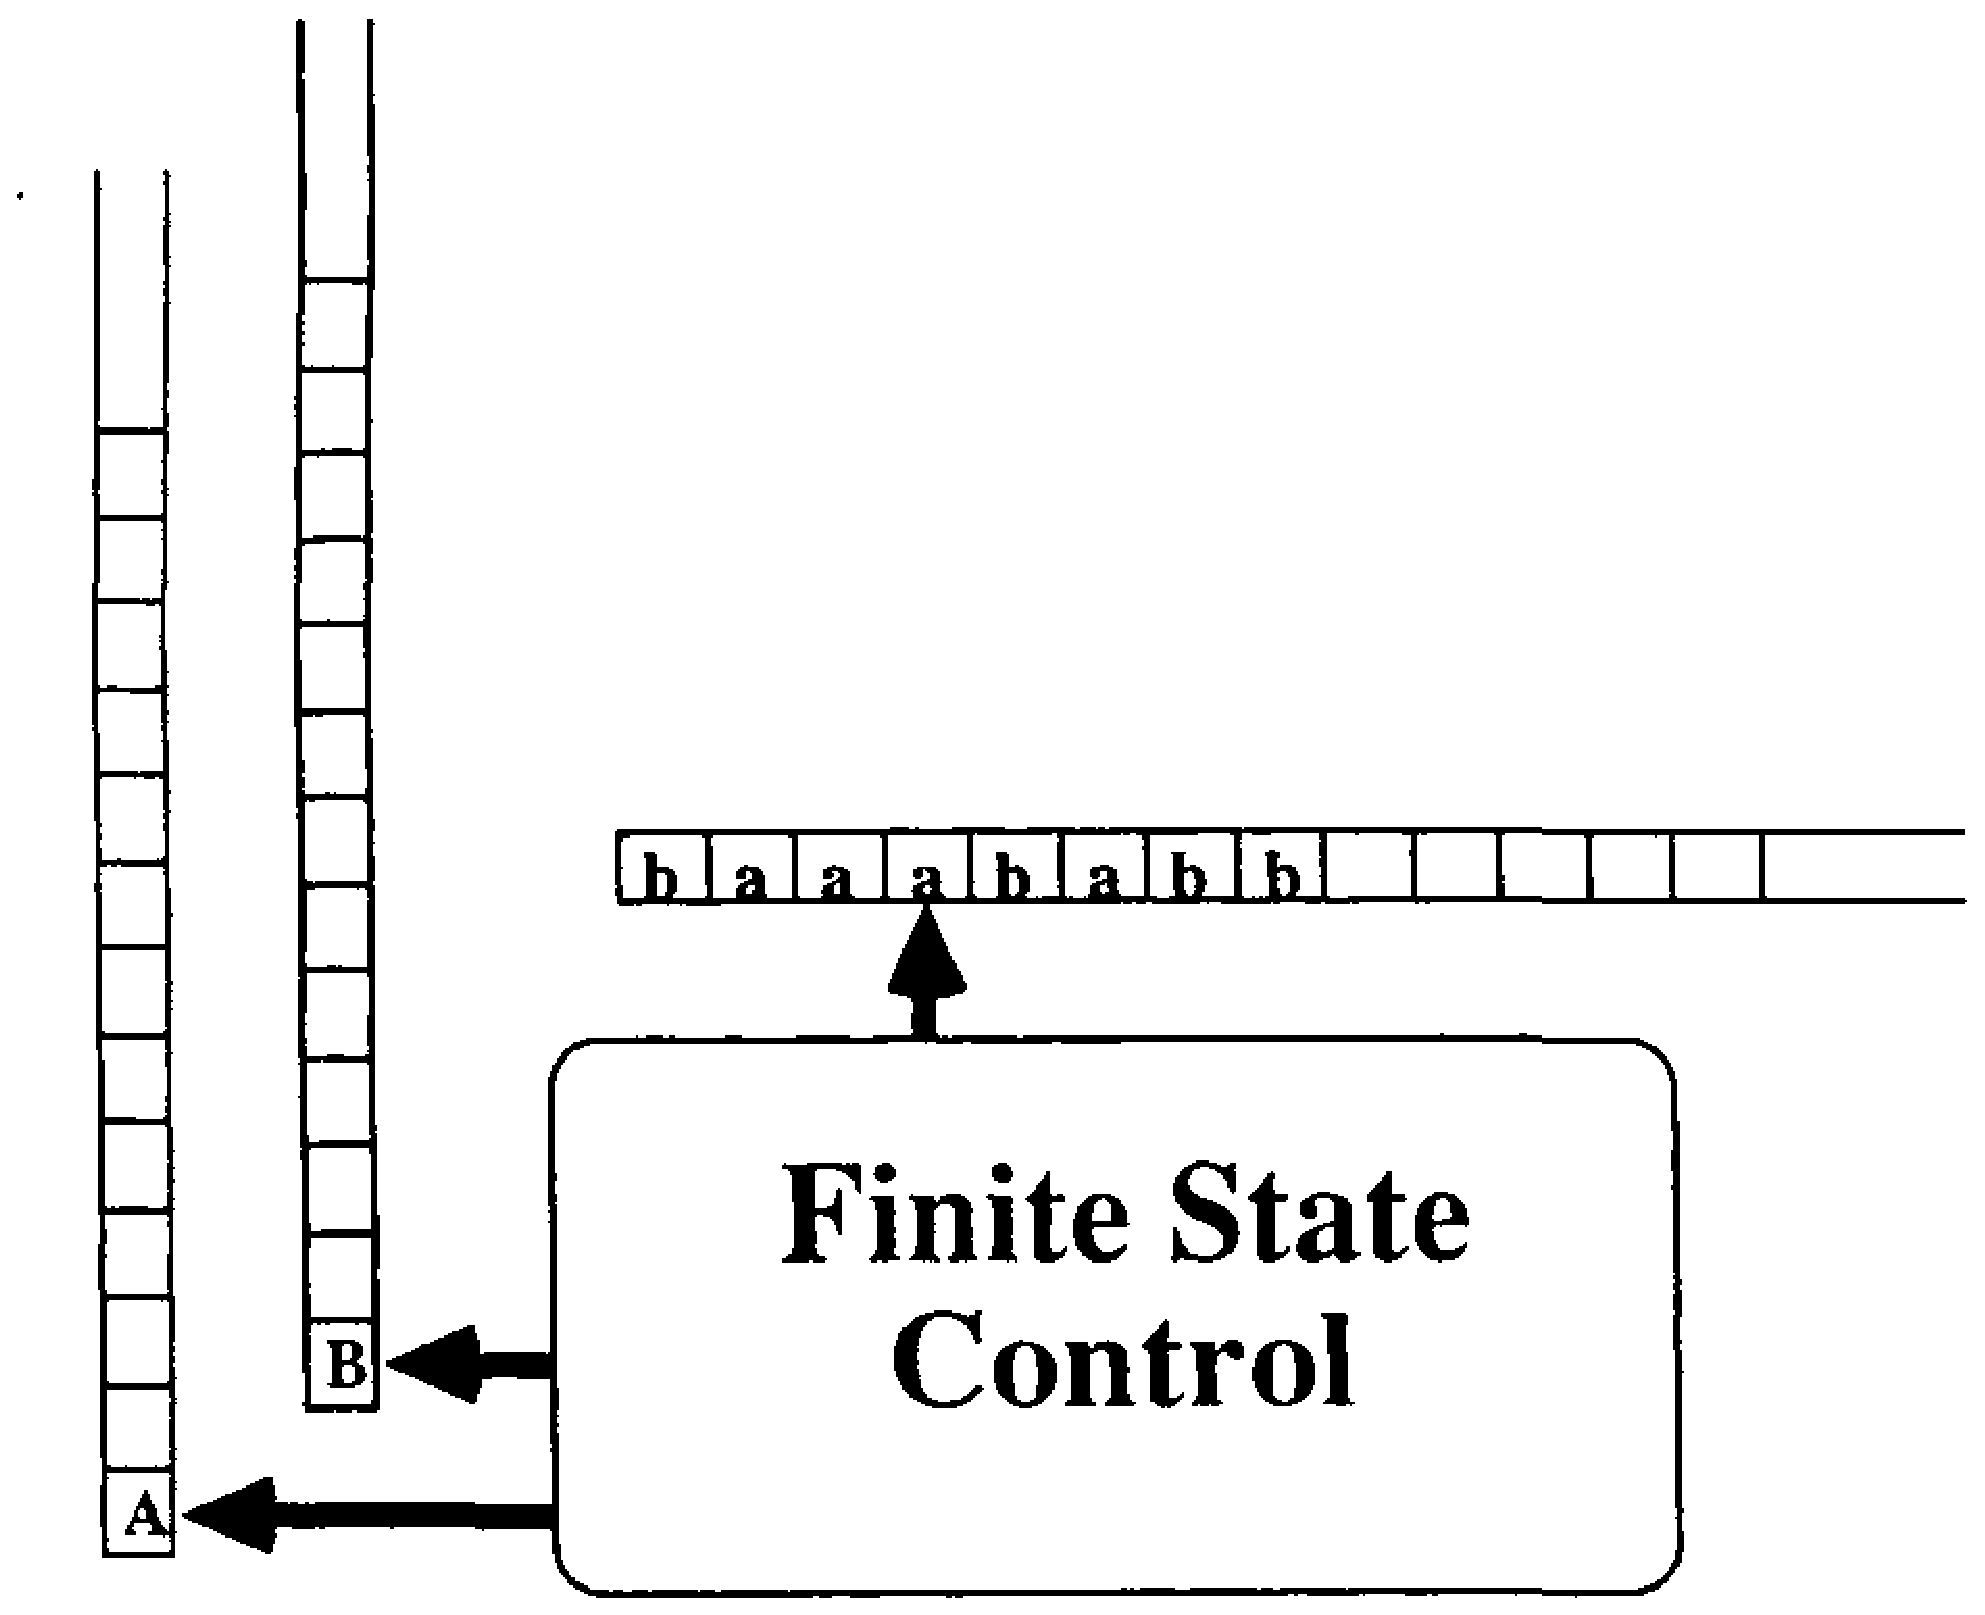
\epsfig{figure=ToFAfigures/fig10-6.eps,height=3.0in}}
\caption{A model of a ``pushdown automaton'' with two tapes}\label{fig-10.6}
\end{figure}

% Theorem 10.6
\begin{thm}\label{thm-10.6}
\CSIG\ is closed under intersection with a regular set. That is, if $L_1$ is
context free and $R_2 $is regular, $L_1\cap R_2$ is always context free.

\emph{Proof.} Let $L_1$ be a context-free language and let $R_2$ be a regular
set. Since $\CSIG=\FSIG$ there must be a PDA $P_1=\langle\Sigma,\Gamma_1,S_1,
s_{0_1},\delta_1,B_1,F_1\rangle$ for which $L_1=L(P_1)$. Let $A_2=\langle\Sigma,
S_2,s_{0_2},\delta_2,F_2\rangle$ be a DFA for which $R_2=L(A_2)$. Define
\[ P^{\cap} = \langle\Sigma,\Gamma_1,S_1\times S_2,\langle s_{0_1},s_{0_2}
	\rangle,\delta^{\cap},B_1,F_1\times F_2\rangle, \]
where $\delta^{\cap}$ is defined by:
\begin{enumerate}
\item $(\forall s_1\in S_1)(\forall s_2\in S_2)(\forall\pmb{a}\in\Sigma)(\forall
	A\in\Gamma_1)$ \\
	$(\delta^{\cap}(\langle s_1,s_2\rangle,\pmb{a},A)=\{\langle\langle t_1,
	t_2\rangle,\beta\rangle\ |\ \langle t_1,\beta\rangle\in\delta_1(s_1,\pmb{a},
	A)\wedge t_2=\delta_2(s_2,\pmb{a})\}).$
\item $(\forall s_1\in S_1)(\forall s_2\in S_2)(\forall A\in\Gamma_1)$ \\
	$(\delta^{\cap}(\langle s_1,s_2\rangle,\lambda,A)=\{\langle\langle t_1,
	t_2\rangle,\beta\rangle\ |\ \langle t_1,\beta\rangle\in\delta_1(s_1,\lambda,A)\wedge t_2
	=s_2\}).$
\end{enumerate}

As with the constructions in the previous sections, induction on the number of
moves exhibits the desired correspondence between the behaviors of the machines.
In particular, it can be shown for any $\alpha,\beta\in\Gamma^*$ that
\begin{center}\begin{tabular}{l}
$(\forall x\in\Sigma^*)(\forall s_1,t_1\in S_1)(\forall s_2,t_2\in S_2)
	(\langle\langle s_1,s_2\rangle,xy,\alpha\rangle\Dvdash\langle\langle
	t_1,t_2\rangle,y,\beta\rangle\text{ in }P_1\Leftrightarrow$ \\
$((\langle s_1,xy,	\alpha)\Dvdash\langle t_1,y,\beta\rangle\text{ in }
	P^{\cap})\wedge(t_2=\DBAR_2(s_2,x))))$
\end{tabular}\end{center}
From this, with $\alpha=B_1$, $s_1 = s_{0_1}$, $s_2 = s_{0_2}$ and the observation that $\langle t_1,t_2\rangle\in
F_1\times F_2$ $\Leftrightarrow$ $t_1\in F_1\wedge t_2\in F_2$, it follows that $(\forall x\in
\Sigma^*)(x\in L(P^{\cap})\Leftrightarrow (x\in L(P_1)\wedge x\in L(A_2)))$.
Therefore,
\[ L(P^{\cap})=L(P_1)\cap L(A_2)=L_1\cap R_2. \]
Since $P^{\cap}$ is a PDA accepting $L_1\cap R_2$, $L_1\cap R_2$ must be context
free.
\end{thm}

Closure properties such as this are quite useful in showing that certain
languages are not context free. Consider the set $L=\{x\in\{\pmb{a},\pmb{b},
\pmb{c}\}^*|\ \ |x|_{\pmb{a}} = |x|_{\pmb{b}} = |x|_{\pmb{c}}\}$. Since the letters
in a word can occur in any order, a pumping theorem proof is less
straight-forward than for the set $\{\pmb{a}^n\pmb{b}^n\pmb{c}^n|\ n\geq 0\}$.
However, if $L$ were context free, then $L\cap\pmb{a}^*\pmb{b}^*\pmb{c}^*$ would
also be context free (why?). But $L\cap\pmb{a}^*\pmb{b}^*\pmb{c}^*=\{\pmb{a}^n\pmb{b}^n
\pmb{c}^n|\ n\geq 0\}$, and thus $L$ cannot be context free. The exercises suggest
other occasions for which closure properties are useful in showing certain
languages are not context free.

For the machines discussed in the first portion of this text, it was seen that
nondeterminism did not add to the computing power of DFAs. In contrast, this
is not the case for pushdown automata. There are languages that can be accepted
by nondeterministic pushdown automata that cannot be accepted by any
deterministic pushdown automaton. The following is the broadest definition of
what can constitute a deterministic pushdown automaton.

% Definition 10.8
\begin{dfn}\label{dfn-10.8}
A\ \emph{\Index{deterministic pushdown automaton}} (\Index{DPDA}) is a pushdown
automaton\linebreak $P=\langle\Sigma,\Gamma,S,s_0,\delta,B,F\rangle$ with the following
restrictions on the state transition function $\delta$:
\begin{enumerate}
\item $(\forall\pmb{a}\in\Sigma)(\forall A\in\Gamma)(\forall s\in S)(\delta(s,
	\pmb{a},A)$ is empty or contains just one element).
\item $(\forall A\in\Gamma)(\forall s\in S)(\delta(s,\lambda,A)$ is empty or
	contains just one element).
\item $(\forall A\in\Gamma)(\forall s\in S)(\delta(s,\lambda,A)\not=\emptyset
	\Rightarrow (\forall\pmb{a}\in \Sigma)(\delta(s,\pmb{a},A)=\emptyset))$.
\end{enumerate}
\end{dfn}

Rule 1 states that, for a given input letter, deterministic pushdown automata
cannot have two different choices of destination states or two different choices
of strings to place on the stack. Rule 2 ensures that there is no choice of
$\lambda$-moves either. Furthermore, rule 3 guarantees that there will never be
a choice between a $\lambda$-move and a transition that consumes a letter;
states that have a $\lambda$-move can have \emph{only} that one move; no other
transitions of any type are allowed out of that state. Thus, for any string,
there is never any more than one path through the machine. Unlike deterministic
finite automata, deterministic pushdown automata may not always completely
process the strings in $\Sigma^*$; a given string may reach a state that has
no further valid moves, or a string may prematurely empty the stack. In each
case, the DPDA would halt without processing any further input (and reject the string).

\subsection*{Example 10.10}

The automaton $P_1$ in Example 10.1 was deterministic. The PDAs in Examples 10.4
and 10.5 were not deterministic. The automaton $P_G$ derived in Example 10.7 was
not deterministic because there were three possible choices of moves listed
for $\delta_G(s,\pmb{(}, R)$: $\{\langle s,R\cdot R\pmb{)}\rangle,\langle s,R
\cup R\pmb{)}\rangle,\langle s,R\pmb{)^*}\rangle\}$. These choices corresponded
to the three different operators that might have generated the open parenthesis.

Pushdown automata provide an appropriate mechanism for parsing sentences in
programming languages. The regular expression grammar in Example 10.7 is quite
similar to the arithmetic expression grammar that describes expressions in many
programming languages. Indeed, the transitions taken within the corresponding
PDA give an indication of which productions in the underlying grammar were used;
such information is of obvious use in compiler construction. A nondeterministic
pushdown automaton is at best a very inefficient tool for parsing; a DPDA is
much better suited to the task.

As mentioned in the proof of Theorem \ref{thm-10.2}, each leftmost derivation in $G$ has
a corresponding sequence of moves in $P_G$. If $G$ is ambiguous, then there is at
least one word with two distinct leftmost derivations, and hence if that word
appeared on the input tape of $P_G$, there would be two distinct move sequences
leading to acceptance. In this case, $P_G$ cannot possibly be deterministic. On
the other hand, if $P_G$ is nondeterministic, this does not mean that $G$ is
ambiguous, as demonstrated by Example 10.7. In parsing a string in that
automaton, it may not be immediately obvious which production to use (and hence
which transition to take), but for any string, there is at most only one correct
choice; each word has a unique parse tree and a unique leftmost derivation. The
grammar in Example 10.7 is not ambiguous, even though the corresponding PDA was
nondeterministic.

\subsection*{Example 10.11}

The following Greibach normal form grammar is similar to the one used to
construct the PDA in Example 10.7, but with the different operators paired with
unique delimiters. Let
\[ G=\langle\{R\},\{\pmb{a},\pmb{b},\pmb{c},\pmb{(},\pmb{)},\pmb{\{},\pmb{\}},
	\pmb{[},\pmb{]},\pmb{\epsilon},\pmb{\emptyset},\pmb{\cup},\pmb{\cdot},
	\pmb{^*}\},R,\{R\rightarrow\pmb{a}|\pmb{b}|\pmb{c}|\pmb{\epsilon}|
	\pmb{\emptyset}|\pmb{(}R\pmb{\cdot}R\pmb{)}|\pmb{[}R\pmb{\cup}R\pmb{]}|
	\pmb{\{}R\pmb{\}}^*\}\rangle. \]
The automaton $P_G$ is then
\[ \langle\{\pmb{a},\pmb{b},\pmb{c},\pmb{(},\pmb{)},\pmb{\{},\pmb{\}},\pmb{[},
	\pmb{]},\pmb{\epsilon},\pmb{\emptyset},\pmb{\cup},\pmb{\cdot},\pmb{^*}\},
	\{R,\pmb{a},\pmb{b},\pmb{c},\pmb{(},\pmb{)},\pmb{\{},\pmb{\}},\pmb{[},
	\pmb{]},\pmb{\epsilon},\pmb{\emptyset},\pmb{\cup},\pmb{\cdot},\pmb{^*}\},\{s\},s,
	\delta_G,R,\emptyset\rangle \]
where $\delta_G$ is comprised of the following nonempty transitions:
\begin{center}\begin{tabular}{r@{ = }l}
$\delta_G(s,\pmb{(},R)$ & $\{\langle s,R\pmb{\cdot}R\pmb{)}\rangle\}$ \\
$\delta_G(s,\pmb{[},R)$ & $\{\langle s,R\pmb{\cup}R\pmb{]}\rangle\}$ \\
$\delta_G(s,\pmb{\{},R)$ & $\{\langle s,R\pmb{\}^*}\rangle\}$ \\
$\delta_G(s,\pmb{a},R)$ & $\{\langle s,\lambda\rangle\}$ \\
$\delta_G(s,\pmb{b},R)$ & $\{\langle s,\lambda\rangle\}$ \\
$\delta_G(s,\pmb{c},R)$ & $\{\langle s,\lambda\rangle\}$ \\
$\delta_G(s,\pmb{\epsilon},R)$ & $\{\langle s,\lambda\rangle\}$ \\
$\delta_G(s,\pmb{\emptyset}, R)$ & $\{\langle s,\lambda\rangle\}$ \\
$\delta_G(s,\pmb{a},\pmb{a})$ & $\{\langle s,\lambda\rangle\}$ \\
$\delta_G(s,\pmb{b},\pmb{b})$ & $\{\langle s,\lambda\rangle\}$ \\
$\delta_G(s,\pmb{c},\pmb{c})$ & $\{\langle s,\lambda\rangle\}$ \\
$\delta_G(s,\pmb{\emptyset},\pmb{\emptyset})$ & $\{\langle s,\lambda\rangle\}$ \\
$\delta_G(s,\pmb{\epsilon},\pmb{\epsilon})$ & $\{\langle s,\lambda\rangle\}$ \\
$\delta_G(s,\pmb{\cup},\pmb{\cup})$ & $\{\langle s,\lambda\rangle\}$ \\
$\delta_G(s,\pmb{\cdot},\pmb{\cdot})$ & $\{\langle s,\lambda\rangle\}$ \\
$\delta_G(s,\pmb{^*},\pmb{^*})$ & $\{\langle s,\lambda\rangle\}$ \\
$\delta_G(s,\pmb{)},\pmb{)})$ & $\{\langle s,\lambda\rangle\}$ \\
$\delta_G(s,\pmb{]},\pmb{]})$ & $\{\langle s,\lambda\rangle\}$ \\
$\delta_G(s,\pmb{\}},\pmb{\}})$ & $\{\langle s,\lambda\rangle\}$ \\
$\delta_G(s,\pmb{(},\pmb{(})$ & $\{\langle s,\lambda\rangle\}$ \\
$\delta_G(s,\pmb{[},\pmb{[})$ & $\{\langle s,\lambda\rangle\}$ \\
$\delta_G(s,\pmb{\{},\pmb{\{})$ & $\{\langle s,\lambda\rangle\}$
\end{tabular}\end{center}

All other transitions are empty; that is, they are of the form $\delta_G(s,
\pmb{d},A) = \{\ \ \}$. The resulting PDA is clearly deterministic, since there
are no $\lambda$-moves and the other transitions are all singleton sets or are
empty. It is instructive to step through the transitions in $P_G$ for a string
such as $\pmb{[\{(a\cdot b)\}^*\cup c]}$. Upon encountering a delimiter while
scanning a prospective string, the parser would immediately know which operation
gave rise to that delimiter, and need not ``guess'' at which of the three
productions might have been applied. Note that $G$ was an LL0 grammar (as
defined in Section \ref{sec-9.2}), and the properties of $G$ resulted in $P_G$ being a
deterministic device. An efficient parser for this language follows immediately
from the specification of the grammar, whereas the grammar in Example 10.7 gave
rise to a nondeterministic device.

Programmers would not be inclined to tolerate remembering which delimiters
should be used in conjunction with the various operators, and hence programming
language designers take a slightly different approach to the problem. The
nondeterminism in Example 10.7 may only be an effect of the particular grammar
chosen and not inherent in the language itself. Note that the language
$\{\pmb{a}^n\pmb{b}^n|\ n\geq 1\}$ had a grammar that produced a nondeterministic
PDA (Example 10.4), but it also had a grammar that corresponded to a DPDA
(Example 10.1). In compiler construction, designers lean toward syntax that is
compatible with determinism, and they seek grammars for the language that
reflect that determinism.

\subsection*{Example 10.12}

Consider again the language discussed in Example 10.7, which can also be
expressed by the following grammar
\[ H = \langle\{S,T\},\{\pmb{a},\pmb{b},\pmb{c},\pmb{(},\pmb{)},\pmb{\epsilon},
	\pmb{\emptyset},\pmb{\cup},\pmb{\cdot},\pmb{^*}\},S,\{S\rightarrow\pmb{(}ST|
	\pmb{a}|\pmb{b}|\pmb{c}|\pmb{\epsilon}|\pmb{\emptyset},T\rightarrow
	\pmb{\cdot}S\pmb{)}|\pmb{\cup} S\pmb{)}|\pmb{)^*}\}\rangle \]
The automaton $P_H$ is then
\[ \langle\{\pmb{a},\pmb{b},\pmb{c},\pmb{(},\pmb{)},\pmb{\epsilon},
	\pmb{\emptyset},\pmb{\cup},\pmb{\cdot},\pmb{^*}\},\{S,T,\pmb{a},\pmb{b},
	\pmb{c},\pmb{(},\pmb{)},\pmb{\epsilon},\pmb{\emptyset},\pmb{\cup},
	\pmb{\cdot},\pmb{^*}\},\{t\},t,\delta_H,S,\emptyset\rangle \]
where each production of $H$ gives rise to the following transitions in
$\delta_H$:
\begin{center}\begin{tabular}{r@{ = }l}
$\delta_H(t,\pmb{(},S)$ & $\{\langle t,ST\rangle\}$ \\
$\delta_H(t,\pmb{a},S)$ & $\{\langle t,\lambda\rangle\}$ \\
$\delta_H(t,\pmb{b},S)$ & $\{\langle t,\lambda\rangle\}$ \\
$\delta_H(t,\pmb{c},S)$ & $\{\langle t,\lambda\rangle\}$ \\
$\delta_H(t,\pmb{\epsilon},S)$ & $\{\langle t,\lambda\rangle\}$ \\
$\delta_H(t,\pmb{\emptyset},S)$ & $\{\langle t,\lambda\rangle\}$ \\
$\delta_H(t,\pmb{\cdot},T)$ & $\{\langle t,S\pmb{)}\rangle\}$ \\
$\delta_H(t,\pmb{\cup},T)$ & $\{\langle t,S\pmb{)}\rangle\}$ \\
$\delta_H(t,\pmb{)},T)$ & $\{\langle t,\pmb{^*}\rangle\}$
\end{tabular}\end{center}
While the formal definition of $\delta_H$ specifies several productions of the
form $\delta_H(t,\pmb{d},\pmb{d})=\{\langle t,\lambda\rangle\}$, by observing
what can be put on the stack by the above productions, it is clear that the only
remaining useful transitions in $\delta_H$ are
\[ \delta_H(t,\pmb{^*},\pmb{^*})=\{\langle t,\lambda\rangle\} \]
and
\[ \delta_H(t,\pmb{)},\pmb{)})=\{\langle t,\lambda\rangle\} \]

Thus, even though the PDA $P_G$ in Example 10.7 turned out to be nondeterministic,
this was not a flaw in the language itself, since $P_H$ is an equivalent DPDA.
Notice that the grammar $G$ certainly appears to be more straightforward than
$H$. $G$ had fewer nonterminals and fewer productions, and it is a bit harder to
understand the relationships between the nonterminals of $H$. Nevertheless, the
LL0 grammar $H$ led to an efficient parser and G did not.

To take advantage of the resulting reduction in complexity, all major
programming languages are designed to be recognized by DPDAs. These constructs
naturally lead to a mechanical framework for syntactic analysis. In Example
10.12, the application of the production $T\rightarrow\pmb{\cup} S\pmb{)}$ [that is,
the use of the transition $\delta_H(t,\pmb{\cup},T)=\{\langle t,S\pmb{)}\rangle\}$\ ]
signifies that the previous expression and the expression to which $S$ will
expand are to be combined with the union operator. It should be easy to see that
a similar grammar and DPDA for arithmetic expressions (using $+,-,^*$, and $/$
rather than $\cup,\cdot$ and $^*$) would provide a guide for converting such
expressions into their equivalent machine code.

Deterministic pushdown automata have some surprising properties. Recall that
\CSIG\ was not closed under complementation, and since $\PSIG=\CSIG$, there
must be some PDAs that define languages whose complement cannot be recognized by
any PDA. However, it can be shown that any language accepted by a DPDA must have
a complement that can also be recognized by a DPDA. The construction used to
prove this statement, in which final and nonfinal states are interchanged in a
DPDA that accepts via final state, is similar to the approach used in Theorem
\ref{thm-5.1} for deterministic finite automata. It is useful to recall why it was crucial
in the proof of Theorem \ref{thm-5.1} to begin with a DFA when interchanging states,
rather than using an NDFA. Strings that have multiple paths in an NDFA that lead
to both final and nonfinal states would be accepted in the original automaton
and also in the machine with the states interchanged. Furthermore, some strings
may have no complete paths through the NDFA and be rejected in both the original
and new automata. The problem of multiple paths does not arise with DPDAs, since
by definition no choice of moves is allowed. However, strings that do not get
completely consumed would be rejected in both the original DPDA and the DPDA
with final and nonfinal states interchanged. Thus, the proof of closure under
complement for DPDAs is not as straightforward as for DFAs. There are three ways
an input string might not be completely consumed: the stack might empty
prematurely, there may be no transition available at some point, or there might
only be a cycle of $\lambda$-moves available that consumes no further input. The
exercises indicate that it is possible to avoid these problems by padding the
stack with a new bottom-of-the-stack symbol, and adding a ``garbage state'' to
which strings that are hopelessly stuck would transfer.

% Theorem 10.7
\begin{thm}\label{thm-10.7}
If $L$ is a language recognized by a deterministic pushdown automaton, then
$\sim\!\!L$ can also be recognized by a DPDA.

\emph{Proof.} See the exercises.
\end{thm}

% Definition 10.9
\begin{dfn}\label{dfn-10.9}\index{A @\ASIG \ (A-sigma )}
Given any alphabet $\Sigma$, let \ASIG\ represent the collection of all languages
recognized by deterministic pushdown automata. If $L\in\ASIG$, then $L$ is said
to be a \emph{\Index{deterministic context-free language}} (\Index{DCFL}).
\end{dfn}

Theorem \ref{thm-10.7} shows that unlike \PSIG, \ASIG is closed under complementation.
This divergent behavior has some immediate consequences, as stated below.

% Theorem 10.8
\begin{thm}\label{thm-10.8}
Let $\Sigma$ be an alphabet.
\begin{quote}
If \ $|\Sigma|=1$, then $\DSIG = \ASIG = \PSIG$. \\
If \ $|\Sigma|>1$, then \DSIG\ is properly contained in \ASIG, which is properly
contained in \PSIG.
\end{quote}

\emph{Proof.} For every alphabet $\Sigma$, examining the proof of Theorem \ref{thm-10.1}
shows that every finite automaton has an equivalent deterministic pushdown
automaton, and thus it is always true that $\DSIG\subseteq\ASIG$. Definition
\ref{dfn-10.7} implies that $\ASIG\subseteq\PSIG$. If $|\Sigma|=1$, then Theorem \ref{thm-9.15}
showed that $\DSIG = \CSIG\  ( = \PSIG)$, from which it follows that $\DSIG =
\ASIG = \PSIG$. If\, $|\Sigma|>1$, an example such as $\{\pmb{a}^n\pmb{b}^n|\,n\geq
1\}$ shows that \DSIG\ is properly contained in \ASIG\ (see the exercises).
Since $\mathfrak{P}_{\{\pmb{a},\pmb{b}\}}$ and $\cal{A}_{\{\pmb{a},
\pmb{b}\}}$ have different closure properties, they cannot represent the same
collection, and $\ASIG\subseteq\PSIG$ implies that the containment must be
proper.
\end{thm}

In the proof of Theorem \ref{thm-10.6}, it is easy to see that if $P_1$ is deterministic
then $P^{\cap}$ will be a DPDA, also. Hence \ASIG, like \PSIG, is closed under
intersection with a regular set. Also, the exercises show that both \ASIG\ and
\PSIG\ are closed under difference with a regular set. However, the closure
properties of \ASIG\ and \PSIG\  disagree in just about every other case. The
languages
\[ L_1 = \{\pmb{a}^n\pmb{b}^m|\ (n \geq 1)\wedge(n = m)\}\qquad\text{and}\qquad
	L_2 = \{\pmb{a}^n\pmb{b}^m|\ (n \geq 1)\wedge(n = 2m)\} \]
are both DCFLs, and yet $L_1\cup L_2 = \{\pmb{a}^n\pmb{b}^m|\ (n \geq 1)\wedge(n=
m \vee n = 2m)\}$ is not a DCFL (see the exercises). Thus, unlike \PSIG, \ASIG\ 
is not closed under union if $\Sigma$ is comprised of at least two symbols
(recall that since $\mathfrak{D}_{\{\pmb{a}\}} = \cal{A}_{\{\pmb{a}\}} =
\mathfrak{P}_{\{\pmb{a}\}}$, $\cal{A}_{\{\pmb{a}\}}$ would be closed under
union). If \ASIG\ was closed under intersection, then \ASIG\ would (by
De~Morgan's law) be closed under union, since it is closed under complement. Hence,
\ASIG\ cannot be closed under intersection.

The language $\{\pmb{c}^n\pmb{b}^m|\ (n \geq 1)\wedge(n=m)\}\cup\{\pmb{a}^n
\pmb{b}^m|\ (n \geq 1)\wedge(n=2m)\}$ is definitely a DCFL, and yet a simple
homomorphism can transform it into
\[ \{\pmb{a}^n\pmb{b}^m|\ (n\geq 1)\wedge((n=m)\vee(n=2m))\} \]
(see the exercises). Thus, \ASIG\ is not closed under homomorphism. Since
homomorphisms are special cases of substitutions, \ASIG\ is not closed under
substitution either. \ASIG\ is also the only collection of languages discussed
in this text that is not closed under reversal; $\{\pmb{ca}^n\pmb{b}^m|\ (n\geq 1)
\wedge(n=m)\}\cup\{\pmb{a}^n\pmb{b}^m|\ (n\geq 1)\wedge(n=2m)\}$ is a DCFL, but
$\{\pmb{b}^m\pmb{a}^n\pmb{c}\ |\ (n\geq 1)\wedge(n=m)\}\cup\{\pmb{b}^m\pmb{a}^n|\ (n
\geq 1)\wedge(n=2m)\}$ is not. These properties are summed up in the following
statements.

% Theorem 10.9
\begin{thm}\label{thm-10.9}
Given any alphabet $\Sigma$, \ASIG\ is closed under complement. \ASIG\ is also
closed under union, intersection, and difference \emph{with a regular set}. That
is, if $L_1$ is a DCFL and $R_2$ is a FAD language, then the following are
deterministic, context-free languages:
\begin{center}\begin{tabular}{c}
$\sim\!\!L_1$ \\
$L_1 \cap R_2$ \\
$L_1 \cup R_2$ \\
$L_1 - R_2$ \\
$R_2 - L_1$
\end{tabular}\end{center}

\emph{Proof.} The proof follows from the above discussion and theorems and the
exercises.
\end{thm}

% Lemma 10.1
\begin{lmm}\label{lmm-10.1}
Let $\Sigma$ be an alphabet comprised of at least two symbols. Then \ASIG\ is
not closed under union, intersection, concatenation, \Index{Kleene closure},
homomorphism, substitution, or reversal. That is, there are examples of
deterministic context-free languages $L_1$ and $L_2$, a homomorphism $h$, and a
substitution $s$ for which the following are not DCFLs:
\begin{center}\begin{tabular}{l}
$L_1 \cup L_2$ \\
$L_1 \cap L_2$ \\
$L_1 \cdot L_2$ \\
$L^*_1$ \\
$\overline{h}(L_1)$ \\
$\overline{s}(L_1)$ \\
$L^r_1$
\end{tabular}\end{center}

\emph{Proof.} The proof follows from the above discussion and theorems and the
exercises.
\end{lmm}

\subsection*{Example 10.13}

These closure properties can often be used to justify that certain languages are
not DCFLs. For example, the language
\[ L = \{x\in\{\pmb{a},\pmb{b},\pmb{c}\}^*|\ \ |x|_{\pmb{a}} = |x|_{\pmb{b}}\}\cup
	\{x\in\{\pmb{a},\pmb{b},\pmb{c}\}^*|\ \ |x|_{\pmb{b}} = |x|_{\pmb{c}}\} \]
can be recognized by a PDA but not by a DPDA. If $L$ were a DCFL, then
$\sim\!\!L = \{x\in\{\pmb{a},\pmb{b},\pmb{c}\}^*|\ \ |x|_{\pmb{a}} \not= |x|_{
\pmb{b}}\}\cap\{x\in\{\pmb{a},\pmb{b},\pmb{c}\}^*|\ \ |x|_{\pmb{b}} \not= |x|_{
\pmb{c}}\}$ would also be a DCFL. However, $\sim\!\!L\cap\pmb{a}^*\pmb{b}^*
\pmb{c}^* = \{\pmb{a}^k\pmb{b}^n\pmb{c}^m|\ (k \not= n)\wedge(n \not= m)\}$, which
should also be a DCFL. Ogden's lemma shows that this is not even a CFL (see the
exercises), and hence the original hypothesis that $L$ was a DCFL must be false.
The interested reader is referred to similar discussions in [HOPC] and [DENN].

The restriction that the head scanning the stack tape could only access the
symbol at the top of the stack imposed limitations on the cognitive power of
this class of automata. While the current contents of the top of the stack could
be stored in the finite-state control and be remembered after the stack was
popped, only a finite number of such pops can be recorded within the states of
the PDA. At some point, seeking information further down on the stack will cause
an irretrievable loss of information. One might suspect that if popped items
were not erased (so that they could be revisited and reviewed at some later
point) a wider class of languages might be recognizable. Generalized automata
that allow such nondestructive ``backtracking'' are called Turing machines and
form a significantly more powerful class of automata. These devices and their
derivatives are the subject of the next chapter.

\section*{Exercises}
\begin{enumerate}[{10.}1.]
\item Refer to Theorem \ref{thm-10.1} and use induction to show
\[ (\forall x\in\Sigma^*)(\DBAR(s_0,x) = t \Leftrightarrow \langle s_0,x,\cent
	\rangle\Dvdash\langle t,\lambda,\cent\rangle) \]

\item Define a \emph{deterministic} pushdown automaton $P'_1$ with only one
state for which $\Lambda(P'_1) = \{\pmb{a}^n\pmb{b}^n|\ n \geq 1\}$.

\item Consider the pushdown automaton defined by $P'_2 = \langle\{\pmb{a},
\pmb{b}\},\{S,C\},\{t\},t,\delta,S,\{t\}\rangle$, where $\delta$ is defined by
\begin{center}\begin{tabular}{r@{ = }l}
$\delta(t,\pmb{a},S)$ & $\{\langle t,SC\rangle,\langle t,C\rangle\}$ \\
$\delta(t,\pmb{a},C)$ & $\{\ \ \}$ \\
$\delta(t,\pmb{b},S)$ & $\{\ \ \}$ \\
$\delta(t,\pmb{b},C)$ & $\{\langle t,\lambda\rangle\}$
\end{tabular}\end{center}
\begin{enumerate}
\item Give an inductive proof that
\[ (\forall i\in\NN)(\langle t,\pmb{a}^i,S\rangle\Dvdash\langle t,\lambda,\alpha
	\rangle \Rightarrow (\alpha=SC^i\vee\alpha=C^i)) \]
\item Give an inductive proof that
\[ (\forall i\in\NN)(\langle t,x,C^i\rangle\Dvdash\langle t,\lambda,\beta\rangle
	\Rightarrow (x=\pmb{b}^i)) \]
\item Find $L(P'_2)$; use parts (a) and (b) to rigorously justify your
statements.
\end{enumerate}

\item Let $L=\{\pmb{a}^i\pmb{b}^j\pmb{c}^k|\ i,j,k\in\NN$ and $i+j=k\}$.
\begin{enumerate}
\item Find a pushdown automaton (which accepts via final state) that recognizes
$L$.
\item Find a pushdown automaton (which accepts via empty stack) that recognizes
$L$.
\item Is there a counting automaton that accepts $L$?
\item Is there a DPDA that accepts $L$?
\item Use Definition \ref{dfn-10.7} to find a grammar equivalent to the PDA in part (a).
\end{enumerate}

\item Let $L=\{x\in\{\pmb{a},\pmb{b},\pmb{c}\}^*|\ \ |x|_{\pmb{a}}+|x|_{\pmb{b}}=
|x|_{\pmb{c}}\}$.
\begin{enumerate}
\item Find a pushdown automaton (which accepts via final state) that recognizes
$L$.
\item Find a pushdown automaton (which accepts via empty stack) that recognizes
$L$.
\item Is there a counting automaton that accepts $L$?
\item Is there a DPDA that accepts $L$?
\item Use Definition \ref{dfn-10.7} to find a grammar equivalent to the PDA in part (a).
\end{enumerate}

\item Prove or disprove that:
\begin{enumerate}
\item \PSIG\ is closed under inverse homomorphism.
\item \ASIG\ is closed under inverse homomorphism.
\end{enumerate}

\item Give an example of a finite language that cannot be recognized by any
one-state PDA that accepts via final state.

\item Let $L=\{\pmb{a}^n\pmb{b}^n\pmb{c}^m\pmb{d}^m|\ n,m\in\NN\}$.
\begin{enumerate}
\item Find a pushdown automaton (which accepts via final state) that recognizes
$L$.
\item Find a pushdown automaton (which accepts via empty stack) that recognizes
$L$.
\item Is there a DPDA that accepts $L$?
\item Is there a counting automaton that accepts $L$?
\item Use Definition \ref{dfn-10.7} to find a grammar equivalent to the PDA in part (b).
\end{enumerate}

\item Refer to Theorem \ref{thm-10.2} and use induction on the number of moves in a
sequence to show that
\[ (\forall x\in\Sigma^*)(\forall\beta\in(\Sigma\cup\Omega)^*)(\langle s,x,S\rangle
	\Dvdash\langle s,\lambda,\beta\rangle \ \ \  \Leftrightarrow\ \ \  S\ 
	\DRightarrow x\beta\text{ as a leftmost derivation}) \]

\item Consider the grammar
\[ \langle\{R\},\{\pmb{a},\pmb{b},\pmb{c},\pmb{(},\pmb{)},\pmb{\epsilon},
	\pmb{\emptyset},\pmb{\cup},\pmb{\cdot},\pmb{^*}\},R,\{R\rightarrow
	\pmb{a}|\pmb{b}|\pmb{c}|\pmb{\epsilon}|\pmb{\emptyset}|\pmb{(}R
	\pmb{\cdot}R\pmb{)}|\pmb{(}R\pmb{\cup}R\pmb{)}|R\pmb{^*}\}\rangle \]
\begin{enumerate}
\item Convert this grammar to Greibach normal form, adding the new nonterminal
$Y$.
\item Use Definition \ref{dfn-10.6} on part (a) to find the corresponding PDA.
\item Use the construct suggested by Theorem \ref{thm-10.4} in part (b) to find the
corresponding PDA that accepts via final state.
\end{enumerate}

\item Let $L=\{\pmb{a}^i\pmb{b}^j\pmb{c}^	j\pmb{d}^i|\ i,j\in\NN\}$.
\begin{enumerate}
\item Find a pushdown automaton (which accepts via final state) that recognizes
$L$.
\item Find a pushdown automaton (which accepts via empty stack) that recognizes
$L$.
\item Is there a DPDA that accepts $L$?
\item Is there a counting automaton that accepts $L$?
\item Use Definition \ref{dfn-10.7} to find a grammar equivalent to the PDA in part (b).
\end{enumerate}

\item Consider the PDA $P_3$ in Example 10.5. Use Definition \ref{dfn-10.7} to find
$G_{P_3}$.

\item Refer to Theorem \ref{thm-10.3} and use induction to show
\[ (\forall x\in\Sigma^*)(\forall A\in\Gamma)(\forall s\in S)(\forall t\in S)
	(A^{st}\,\DRightarrow x\ \ \  \Leftrightarrow\ \ \  \langle s,x,A\rangle\Dvdash\langle
	t,\lambda,\lambda\rangle) \]

\item Let $L=\{\pmb{a}^n\pmb{b}^n\pmb{c}^m\pmb{d}^m|\ n,m\in\NN\}\cup\{\pmb{a}^i
\pmb{b}^j\pmb{c}^j\pmb{d}^i|\ i,j\in\NN\}$.
\begin{enumerate}
\item Find a pushdown automaton (which accepts via final state) that recognizes
$L$.
\item Find a pushdown automaton (which accepts via empty stack) that recognizes
$L$.
\item Is there a DPDA that accepts $L$?
\item Is there a counting automaton that accepts $L$?
\item Use Definition \ref{dfn-10.7} to find a grammar equivalent to the PDA in part (b).
\end{enumerate}

\item Consider the PDA $P_G$ in Example 10.6. Use Definition \ref{dfn-10.7} to find
$G_{P_G}$.

\item Refer to Theorem \ref{thm-10.4} and use induction to show
\[ (\forall\alpha,\beta\in\Gamma^*)(\forall x,y\in\Sigma^*)(\langle s,xy,\alpha\rangle
	\Dvdash\langle s,y,\beta\rangle\text{ in }P \ \ \  \Leftrightarrow\ \ \ \langle s,xy,
	\alpha Y\rangle\Dvdash\langle s,y,\beta Y\rangle\text{ in }P_{\!\!f}) \]

\item Refer to Theorem \ref{thm-10.5} and use induction to show
\[ (\forall \alpha,\beta\in\Gamma^*)(\forall x,y\in\Sigma^*)(\forall s,t\in S)
	(\langle s,xy,\alpha\rangle\Dvdash\langle t,y,\beta\rangle\text{ in }P
	 \ \ \  \Leftrightarrow\ \ \ \langle s,xy,\alpha Y\rangle\Dvdash\langle t,y,\beta Y\rangle
	\text{ in }P_{\lambda}) \]

\item Prove that $\{x\in\{\pmb{a},\pmb{b},\pmb{c}\}^*|\ \ |x|_{\pmb{a}}=|x|_{
\pmb{b}}\wedge|x|_{\pmb{b}} > |x|_{\pmb{c}}\}$ is not context free.
(\emph{Hint:} Use closure properties.)

\item \begin{enumerate}
\item Give an appropriate definition for the state transition function of
the two-tape automaton pictured in Figure \ref{fig-10.6}, stating the new domain and
range.
\item Define a two-tape automaton that accepts $\{\pmb{a}^n\pmb{b}^n\pmb{c}^n|\ n
\geq 1\}$ via final state.
\end{enumerate}

\item \begin{enumerate}
\item Prove that $\{\pmb{a}^n\pmb{b}^n\pmb{c}^n|\ n\geq 1\}$ is not context free.
\item Prove that $\{x\in\{\pmb{a},\pmb{b},\pmb{c}\}^*|\ \ |x|_{\pmb{a}}=|x|_{
\pmb{b}}\}$ is not context free. [\emph{Hint:} Use closure properties and apply
part (a).]
\end{enumerate}

\item \begin{enumerate}
\item Find a DPDA that accepts
\[ \{\pmb{c}^n\pmb{b}^m|\ (n\geq 1)\wedge(n=m)\}\cup\{\pmb{a}^n\pmb{b}^m|\ (n\geq 1)
	\wedge(n=2m)\} \]
\item Define a homomorphism that transforms part (a) into a language that is not
a DCFL.
\end{enumerate}

\item Use Ogden's lemma to show that $\{\pmb{a}^k\pmb{b}^n\pmb{c}^m|\ (k\not=n)
\wedge(n\not=m)\}$ is not a context-free language.

\item Refer to Theorem \ref{thm-10.6} and use induction to show
\begin{center}\begin{tabular}{l}
$(\forall\alpha,\beta\in\Gamma^*)(\forall x\in\Sigma^*)(\forall s_1,t_1\in S_1)
	(\forall s_2,t_2\in S_2)$ \\
$(\langle\langle s_1,s_2\rangle,xy,\alpha\rangle\Dvdash\langle\langle t_1,t_2
	\rangle,y,\beta\rangle$ in $P_1\ \ \ \Leftrightarrow\ \ \ ((\langle s_1,xy,\alpha
	\rangle\Dvdash\langle t_1,y,\beta\rangle$ in $P^{\cap})\wedge(t_2=
	\DBAR_2(s_2,x))))$
\end{tabular}\end{center}

\item Assume that $P$ is a DPDA. Prove that there is an equivalent DPDA $P'$
(which accepts via final state) for which:
\begin{enumerate}
\item $P'$ always has a move for all combinations of states, input symbols, and
stack symbols.
\item $P'$ never empties its stack.
\item For each input string presented to $P'$, $P'$ always scans the entire
input string.
\end{enumerate}

\item Assume the results of Exercise 10.24, and show that \ASIG\ is closed under
complementation. (\emph{Hint:} Exercise 10.24 almost allows the trick of
switching final and nonfinal states to work; the main remaining problem involves
handling the case where a series of $\lambda$-moves may cycle through both final
and nonfinal states.)

\item Give an example that shows that \ASIG\ is not closed under concatenation.

\item Give an example that shows that \ASIG\ is not closed under Kleene closure.

\item Show that $\{\pmb{ca}^n\pmb{b}^m|\ (n\geq 1)\wedge(n=m)\}\cup\{\pmb{a}^n
\pmb{b}^m|\ (n\geq 1)\wedge(n=2m)\}$ is a DCFL.

\item \begin{enumerate}
\item Modify the proof of Theorem \ref{thm-10.6} to show that if $L_1$ is context free and
$R_2$ is regular, $L_1-R_2$ is always context free.
\item Prove the result in part (a) by instead appealing to closure properties
for complement and intersection.
\end{enumerate}

\item \begin{enumerate}
\item Modify the proof of Theorem \ref{thm-10.6} to show that if $L_1$ is context free and
$R_2$ is regular, $L_1\cup R_2$ is always context free.
\item Prove the result in part (a) by instead appealing to closure properties
for complement and intersection.
\end{enumerate}

\item Argue that if $L_1 $is a DCFL and $R_2$ is regular, $R_2-L_1$ is always a
DCFL.

\item \begin{enumerate}
\item Prove that $\{w2w^r|\ w\in\{\pmb{0},\pmb{1}\}^*\}$ is a DCFL.
\item Prove that $\{ww^r|\ w\in\{\pmb{0},\pmb{1}\}^*\}$ is \emph{not} a DCFL.
\end{enumerate}

\item Give examples to show that even if $L_1$ and $L_2$ are DCFLs:
\begin{enumerate}
\item $L_1\cdot L_2$ need not be a DCFL.
\item $L_1-L_2$ need not be a DCFL.
\item $L^*_1$ need not be a DCFL.
\item $L^r_1$ need not be a DCFL.
\end{enumerate}

\item Consider the quotient operator $/$ given by Definition \ref{dfn-5.10}. Prove or
disprove that:
\begin{enumerate}
\item \PSIG\ is closed under quotient.
\item \ASIG\ is closed under quotient.
\end{enumerate}

\item Consider the operator $b$ defined in Theorem \ref{thm-5.11}. Prove or disprove
that:
\begin{enumerate}
\item \PSIG\ is closed under the operator $b$.
\item \ASIG\ is closed under the operator $b$.
\end{enumerate}

\item Consider the operator $Y$ defined in Theorem \ref{thm-5.7}. Prove or disprove that:
\begin{enumerate}
\item \PSIG\ is closed under the operator $Y$.
\item \ASIG\ is closed under the operator $Y$.
\end{enumerate}

\item Consider the operator $P$ given in Exercise 5.16. Prove or disprove that:
\begin{enumerate}
\item \PSIG\ is closed under the operator $P$.
\item \ASIG\ is closed under the operator $P$.
\end{enumerate}

\item Consider the operator $F$ given in Exercise 5.19. Prove or disprove that:
\begin{enumerate}
\item \PSIG\ is closed under the operator $F$.
\item \ASIG\ is closed under the operator $F$.
\end{enumerate}
\end{enumerate}

% Chapter, Section, Theorem, Corollary, Lemma, Definition, Table, Figure, {\bf
\chapter{Turing Machines}\label{ch-11}

In the preceding chapters, we have seen that DFAs and NDFAs represented
the type 3 languages and pushdown automata represented the type 2
languages. In this chapter we will explore the machine analog to
the type 1 and type 0 grammars.  These devices, called \emph{Turing
machines}, are the most powerful automata known and can recognize
every language considered so far in this text. We will also encounter
languages that are too complex to be recognized by any Turing
machine. Indeed, we will see that any other such (finite) scheme
for the representation of languages is likewise forced to be unable
to represent all possible languages over a given alphabet. Turing
machines provide a gateway to \emph{undecidability}, discussed in the next
chapter, and to the general theory of \emph{computational complexity},
which is rich enough to warrant much broader treatment than would
be possible here.

% 11.1 DEFINITIONS AND EXAMPLES
\section{Definitions and Examples}\label{sec-11.1}

Pushdown automata turned out to be the appropriate cognitive devices
for the type 2 languages, but further enhancements in the capabilities
of the automaton model are necessary to achieve the generality
inherent in type 0 and type 1 languages. A (seemingly) minor
modification will be all that is required. \emph{Turing machines} are
comprised of the familiar components that have already been used
in previous classes of automata. As with the earlier constructions,
the heart of the device is a finite-state control, which reacts to
information scanned by the tape head(s).  Like finite-state transducers
and pushdown automata, information can be written\index{read/write head} to tape as
transitions between states are made. Unlike FSTs and PDAs, Turing
machines have only one tape with which to work, which serves both
the input and the output needs of the device. Note that with
finite-state transducers the presence of a second tape was purely
for convenience; a single tape, with input symbols overwritten by
the appropriate output symbol as the read head progressed, would
have sufficed.  Whereas a pushdown automaton could write an entire
string of symbols to the stack, a Turing machine is constrained to
print a single letter at a time.  These new devices would therefore
be of less value than PDAs were they not given some other capability.
In all previous classes of automata, the read head was forced to
move one space to the right on each transition (or, in the case of
$\lambda$-moves, remain stationary).  On each transition, the Turing machine
tape head has the option of staying put, moving right, or moving
left. The ability to move back to the left and review previously
written information accounts for the added power of Turing machines.

It is possible to view a Turing machine as a powerful transducer
of computable functions, with an associated function defined much
like those for FSTs. That is, as with finite-state transducers,
each word that could be placed on an otherwise blank tape is
associated with the word formed by allowing the Turing machine to
operate on that word. With FSTs, this function was well defined;
the machine would process each letter of the word in a unique way,
the read head would eventually find the end of the word (that is,
it would scan a blank), and the device would then halt.  With Turing
machines, there is no built-in guarantee that it will always halt;
since the tape head can move both right and left, it is possible
to define a Turing machine that would reverberate back and forth
between two adjacent spaces indefinitely. A Turing machine is also
not constrained to halt when it scans a blank symbol; it may overwrite
the blank and/or continue moving right indefinitely.

Rather than viewing a Turing machine as a transducer, we will
primarily be concerned with employing it as an acceptor of words
placed on the tape. Some variants of Turing machines are defined
with a set of final states, and the criteria for acceptance would
then be that the device both halt and be in a final state.  For our
purposes, we will employ the writing capabilities of the Turing
machine and simply require that acceptance be indicated by printing
a $\pmb{Y}$ just prior to halting. If such a $\pmb{Y}$ is never printed or the
machine does not halt, the word will be considered rejected.  It
may be that there are words that might be placed on the input tape
that would prevent the machine from halting, which is at best a
serious inconvenience; if the device has been operating for an
extraordinary amount of time, we may not be able to tell if it will
never halt (and thus reject the word), or whether we simply need
to be patient and wait for it to eventually print the $\pmb{Y}$. This
uncertainty can in some cases be avoided by finding a superior
design for the Turing machine, which would always halt, printing $\pmb{N}$
when a word is rejected and $\pmb{Y}$ when a word is accepted. This is not
always a matter of being clever in defining the machine; we will
see that there are some languages that are inherently so complex
that this goal is impossible to achieve.

% Figure 11.1
\begin{figure}[tbh]
\centerline{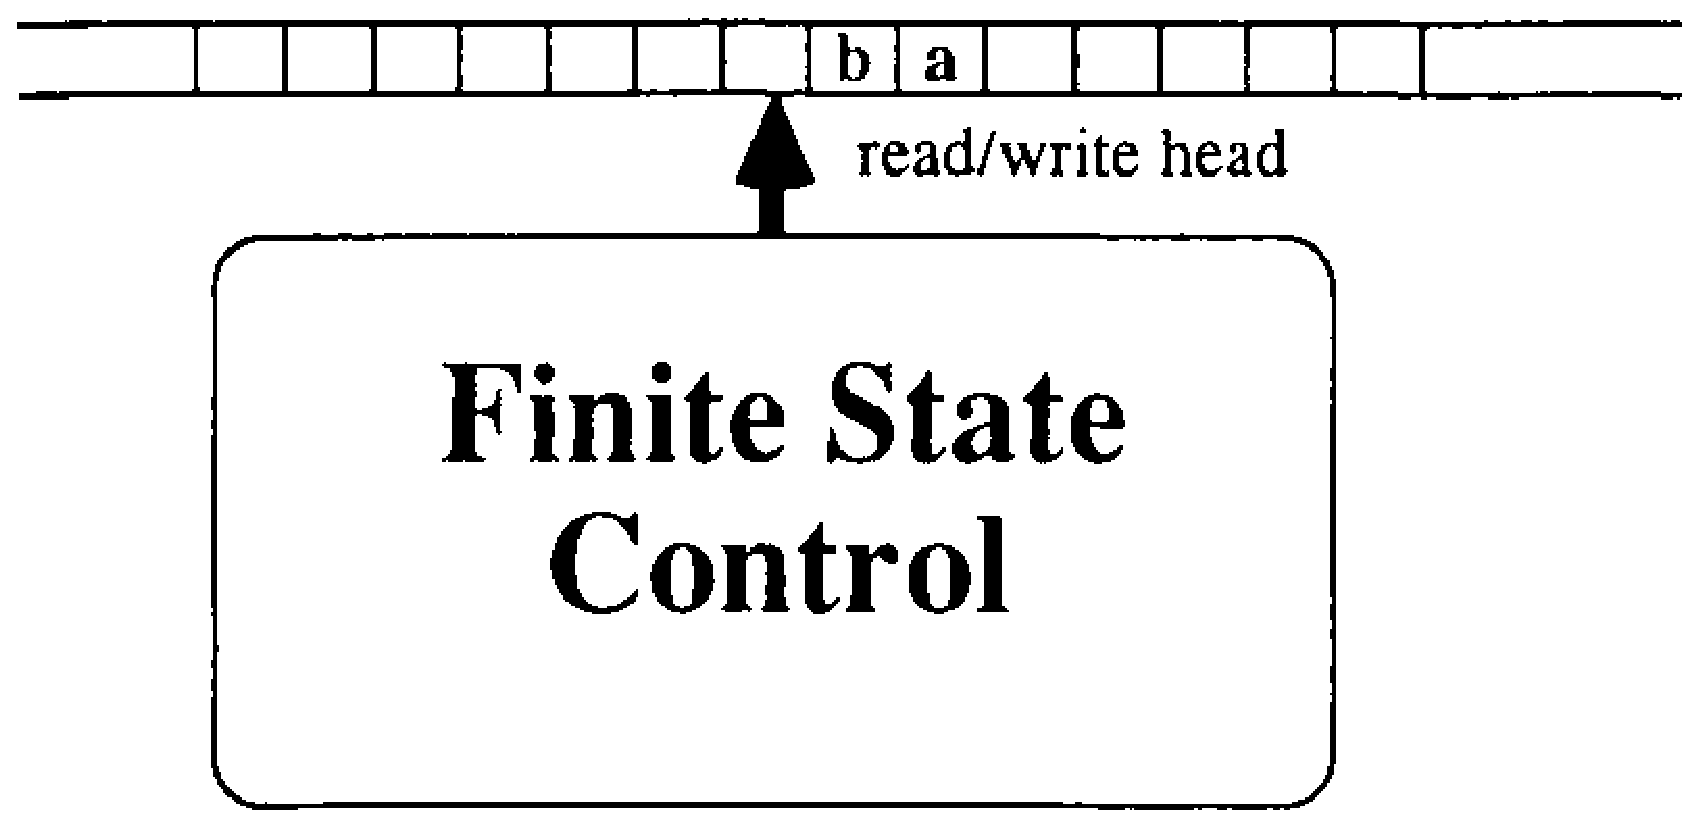
\epsfig{figure=ToFAfigures/fig11-1.eps,width=3.4in}}
\caption{A model of a Turning machine.}\label{fig-11.1}
\end{figure}

A conceptual model of a Turing machine is shown in Figure \ref{fig-11.1}.
Note that the tape head is capable of both reading and overwriting
the currently scanned symbol.  As before, the tape is composed of
a series of cells, with one symbol per cell. The tape head will
also be allowed to move one cell to either the left or right during
a transition. Note that unlike all previous automata, the tape does
not have a ``left end''; it extends indefinitely in both directions.
This tape will be used for input, output, and as a ``scratch pad''
for any intermediate calculations. At the start of operation of the
device, all but a finite number of contiguous cells are blank. Also,
unlike our earlier devices, the following definition implies that
Turing machines may continue to operate after scanning a blank.

% Definition 11.1
\begin{dfn}\label{dfn-11.1}\index{final state!for Turing machine}\index{alphabet!input}\index{alphabet!auxiliary}\index{Turing machine!deterministic}\index{state transition function!for Turing machine}
A \emph{\Index{Turing machine}} that recognizes words over an alphabet $\Sigma$
is a quintuple $M=\langle\Sigma,\Gamma,S,s_0,\delta\rangle$, where

\begin{quote}
$\Sigma$ is the \emph{input alphabet}. \\
$\Gamma$ is the \emph{auxiliary alphabet}, and $\Sigma$, $\Gamma$,
and $\{\pmb{L},\pmb{R}\}$
	are pairwise disjoint sets of symbols. \\
$S$ is a finite nonempty set of \emph{states} (and $S\cap(\Sigma\cup\Gamma) = 
	\emptyset)$. \\
$s_0$ is the \emph{\Index{start state}} $(s_0\in S)$. \\
$\delta$ is the \emph{state transition function} $\delta$: $S\times(\Sigma\cup
	\Gamma)\rightarrow(S\cup\{h\})\times(\Sigma\cup\Gamma\cup\{\pmb{L},\pmb{R}\})$.
\end{quote}
The auxiliary alphabet always includes the \emph{\Index{blank symbol}} (denoted by $\#$),
and neither $\Sigma$ nor $\Gamma$ include the special symbols $\pmb{L}$ and
$\pmb{R}$, which denote moving the tape head left and right, respectively. The
state $h$ is a special \emph{\Index{halt state}}\index{Turing machine!halt state}, from which no further transitions are
possible; $h\notin S$.
\end{dfn}

The alphabet $\Sigma$ is intended to denote the nonblank symbols that can be
expected to be initially present on the input tape. By convention, it is assumed
that the tape head is positioned over the leftmost nonblank (in the case of the
empty string, though, the head will be scanning a blank). In Definition \ref{dfn-11.1},
the state transition function is deterministic; for every state in $S$ and every
tape symbol scanned, exactly one destination state is specified, and one action
is taken by the tape head. The tape head may either:\index{Turing machine!moves}
\begin{enumerate}
\item Overprint the cell with a symbol from $\Sigma$ or $\Gamma$ (and thus a
blank may be printed).
\item Move one cell left (without printing).
\item Move one cell right (also without printing).
\end{enumerate}
In the case where a cell is overprinted, the tape head remains positioned on
that cell.

The above definition of a Turing machine is compatible with the construct
implemented by Jon Barwise and John Etchemendy in their
\Index{Turing's World}$^{\copyright}$ software package for the Apple$^{\text{\textregistered}}$
Macintosh. The Turing's World program allows the user to interactively draw a
state transition diagram of a Turing machine and watch it operate on any given
input string. As indicated by the next example, the same software can be used
to produce and test state transition diagrams for deterministic finite automata.

\subsection*{Example 11.1}

The following simple Turing machine recognizes the set of even-length words
over $\{\pmb{a},\pmb{b}\}$. The state transition diagram for this device is
shown in Figure \ref{fig-11.2} and conforms to the conventions introduced in Chapter \ref{ch-7}.
Transitions between states are represented by arrows labeled by the symbol that
caused the transition. The symbol after the slash denotes the character to be
printed or, in the case of $\pmb{L}$ and $\pmb{R}$, the direction to move the
tape head. The quintuple is $\langle\{\pmb{a},\pmb{b}\},\{\pmb{\#},\pmb{Y},
\pmb{N}\},\{s_0,s_1\},s_0,\delta_T\rangle$, where $\delta_T$ is given by
\begin{center}\begin{tabular}{r@{ = }l}
$\delta_T(s_0,\pmb{a})$ & $\langle s_1,\pmb{R}\rangle$ \\
$\delta_T(s_0,\pmb{b})$ & $\langle s_1,\pmb{R}\rangle$ \\
$\delta_T(s_0,\pmb{\#})$ & $\langle h,\pmb{Y}\rangle$ \\
$\delta_T(s_1,\pmb{a})$ & $\langle s_0,\pmb{R}\rangle$ \\
$\delta_T(s_1,\pmb{b})$ & $\langle s_0,\pmb{R}\rangle$ \\
$\delta_T(s_1,\pmb{\#})$ & $\langle h,\pmb{N}\rangle$
\end{tabular}\end{center}

This particular Turing machine operates in much the same way as a DFA would,
always moving right as it scans each symbol of the word on the input tape.

% Figure 11.2
\begin{figure}
\centerline{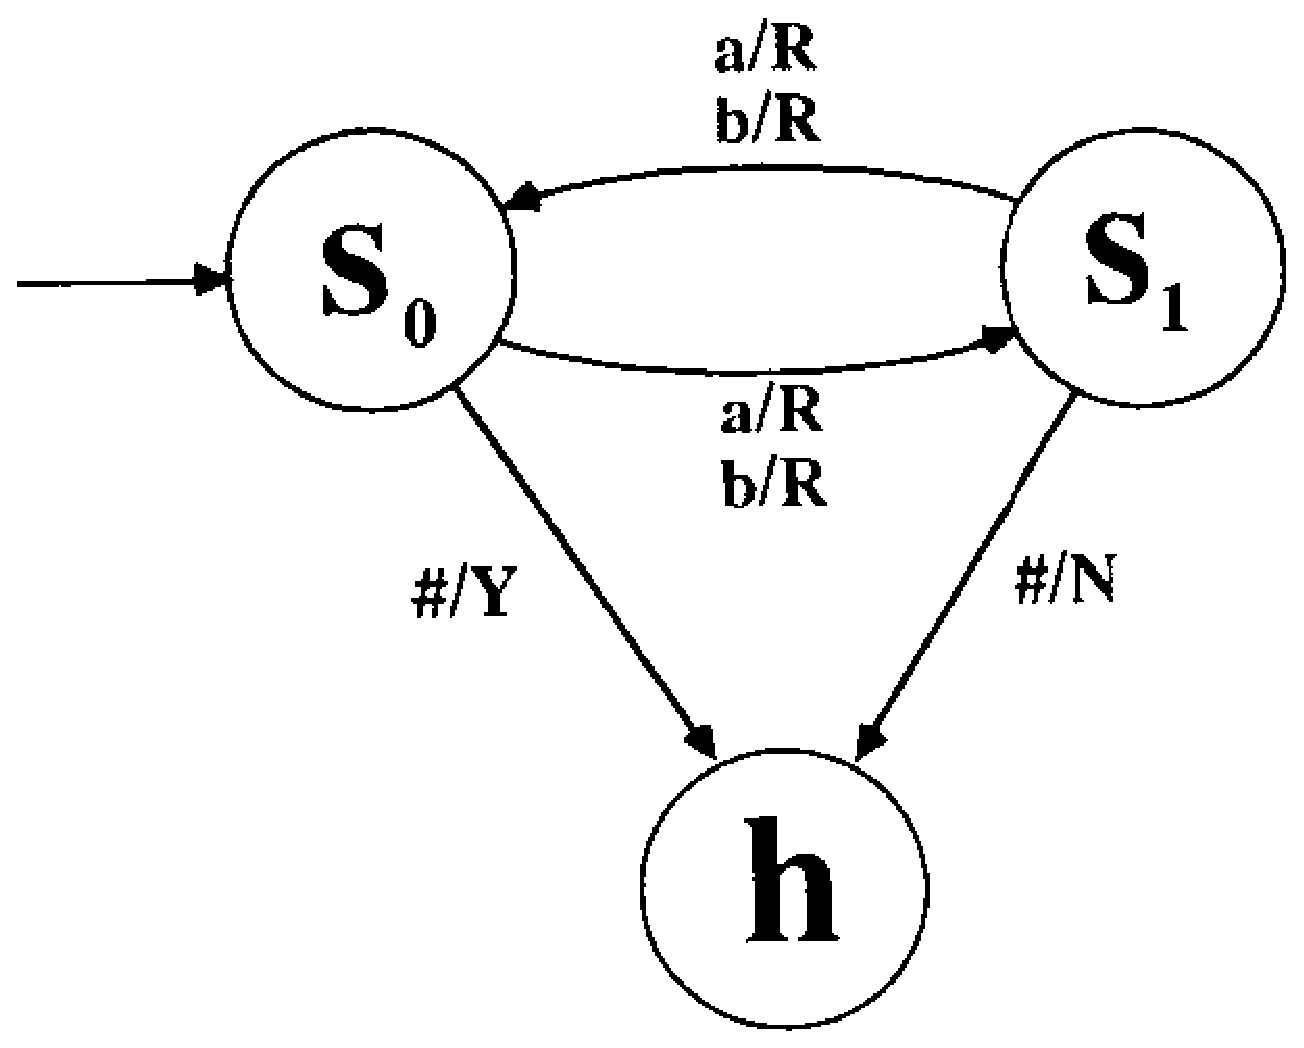
\epsfig{figure=ToFAfigures/fig11-2.eps,width=2.4in}}
\caption{The state transition diagram of the Turing machine discussed in Example
11.1}\label{fig-11.2}
\end{figure}

When it reaches the end of the word (that is, when it first scans a blank), it
prints $\pmb{Y}$ or $\pmb{N}$, depending on which state it is in, and halts. It
differs from a DFA in that the accept/reject indication is printed on the tape
at the right end of the word. Figure \ref{fig-11.3} shows an alternative way of displaying
this machine, in which the halt state is not explicitly shown. Much like the
straight start state arrow that denotes where the automaton is entered, the new
straight arrows show how the machine is left. This notation is especially
appropriate for \emph{\Index{submachines}}. As with complex programs, a complex
Turing machine may be comprised of several submodules. Control may be passed to
a submachine, which manipulates the input tape until it halts. Control may then
be passed to a second submachine, which then further modifies the tape contents.
When this submachine would halt, control may be passed on to a third submachine,
or back to the first submachine, and so on. The straight arrows leaving the
state transition diagram can be thought of as exit arrows for a submachine, and
they function much like a \emph{return} statement in many programming languages.
Example 11.4 illustrates a Turing machine that employs submachines.

% Figure 11.3
\begin{figure}
\centerline{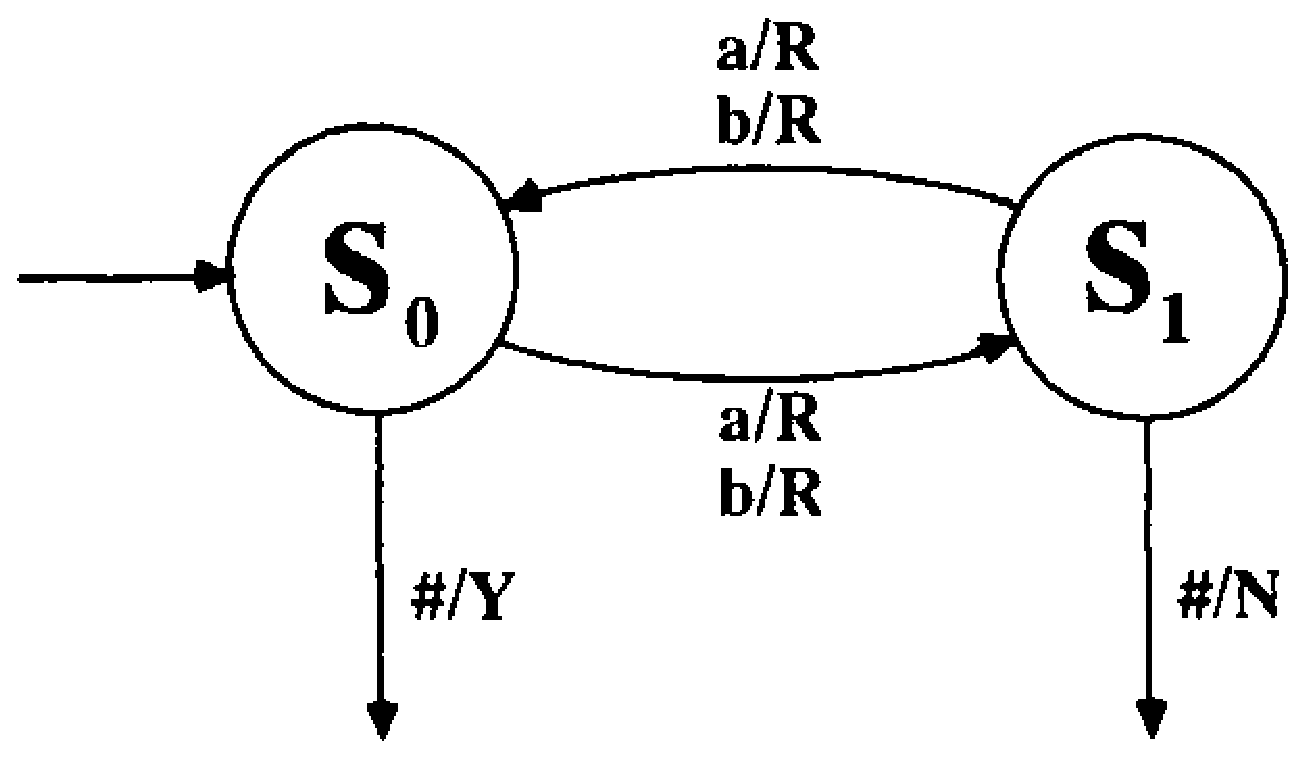
\epsfig{figure=ToFAfigures/fig11-3.eps,width=2.4in}}
\caption{An alternate depiction of the Turing machine discussed in Example 11.1}\label{fig-11.3}
\end{figure}

We will see that any DFA can be emulated by a Turing machine in the manner
suggested by Example 11.1. The following example shows that Turing machines can
recognize languages that are definitely not FAD. In fact, the language accepted
in Example 11.2 is not even context free.

\subsection*{Example 11.2}

The Turing machine $M$ illustrated in Figure \ref{fig-11.4} operates on words over
$\{\pmb{a},\pmb{b},\pmb{c}\}$. When started at the leftmost end of the word, it
is guaranteed to halt at the rightmost end and print $\pmb{Y}$ or $\pmb{N}$. It
happens to overwrite the symbols comprising the input word as it operates, but
this is immaterial. In fact, it is possible to design a slightly more complex
machine that restores the word before halting (see Example 11.11). The quintuple
is $\langle\{\pmb{a},\pmb{b},\pmb{c}\},\{\pmb{\#},\pmb{X},\pmb{Y},\pmb{N}\},\{
s_0,s_1,s_2,s_3,s_4,s_5,s_6\},s_0,\delta\rangle$, where $\delta$ is as indicated
in the diagram in Figure \ref{fig-11.4}. It is intended to recognize the language
$\{x\in\{\pmb{a},\pmb{b},\pmb{c}\}^*|\ \ |x|_{\pmb{a}}=|x|_{\pmb{b}}=|x|_{\pmb{c}}
\}$. One possible procedure for processing a string to check if it had the same
number of $\pmb{a}$s, $\pmb{b}$s, and $\pmb{c}$s is given by the pseudocode
below.

\begin{quote}\begin{tabbing}
aa\=\kill
\emph{while} an $\pmb{a}$ remains \emph{do} \\
\emph{begin} \\
\> replace $\pmb{a}$ by $\pmb{X}$ \\
\> return to leftmost symbol \\
\> find $\pmb{b}$; if none, halt and print $\pmb{N}$ \\
\> replace $\pmb{b}$ by $\pmb{X}$ \\
\> return to leftmost symbol \\
\> find $\pmb{c}$; if none, halt and print $\pmb{N}$ \\
\> replace $\pmb{c}$ by $\pmb{X}$ \\
\> return to leftmost symbol \\
\emph{end} \\
halt and print $\pmb{Y}$ if no more $\pmb{b}$s nor $\pmb{c}$s remain
\end{tabbing}\end{quote}

States $s_0$ and $s_1$ in Figure \ref{fig-11.4} check the \emph{while} condition, and states $s_2$
through $s_6$ perform the body of the do loop. On each iteration, beginning at
the leftmost symbol, state $s_0$ moves the tape head right, checking for symbols
that have not been replaced by $\pmb{X}$. If it reaches the end of the word
(that is, if it scans a blank), the $\pmb{a}$s, $\pmb{b}$s, and $\pmb{c}$s all
matched, and it halts, printing $\pmb{Y}$. If $\pmb{b}$ or $\pmb{c}$ is found,
state 1 searches for $\pmb{a}$s; if the end of the string is reached without
finding a corresponding $\pmb{a}$, the machine halts with $\pmb{N}$, since there
were an insufficient number of $\pmb{a}$s. From either $s_0$ or $s_1$, control
passes to $s_2$ when an $\pmb{a}$ is scanned, and that $\pmb{a}$ is replaced by
$\pmb{X}$. State $s_2$, like $s_4$ and $s_6$, returns the tape head to the
leftmost character. This is done by scanning left until a blank is found and
then moving right as control is passed on to the next state. State $s_3$
searches for $\pmb{b}$, halting with $\pmb{N}$ if none is found. The first
$\pmb{b}$ encountered is otherwise replaced by $\pmb{X}$, and the Turing machine
enters $s_4$, which then passes control on to $s_5$ after returning to the
leftmost symbol. State $s_5$ operates much like $s_3$, searching for $\pmb{c}$
this time, and $s_6$ returns the tape head to the extreme left if the previous
$\pmb{a}$ and $\pmb{b}$ have been matched with $\pmb{c}$. The process then
repeats from $s_0$.

% Figure 11.4
\begin{figure}
\centerline{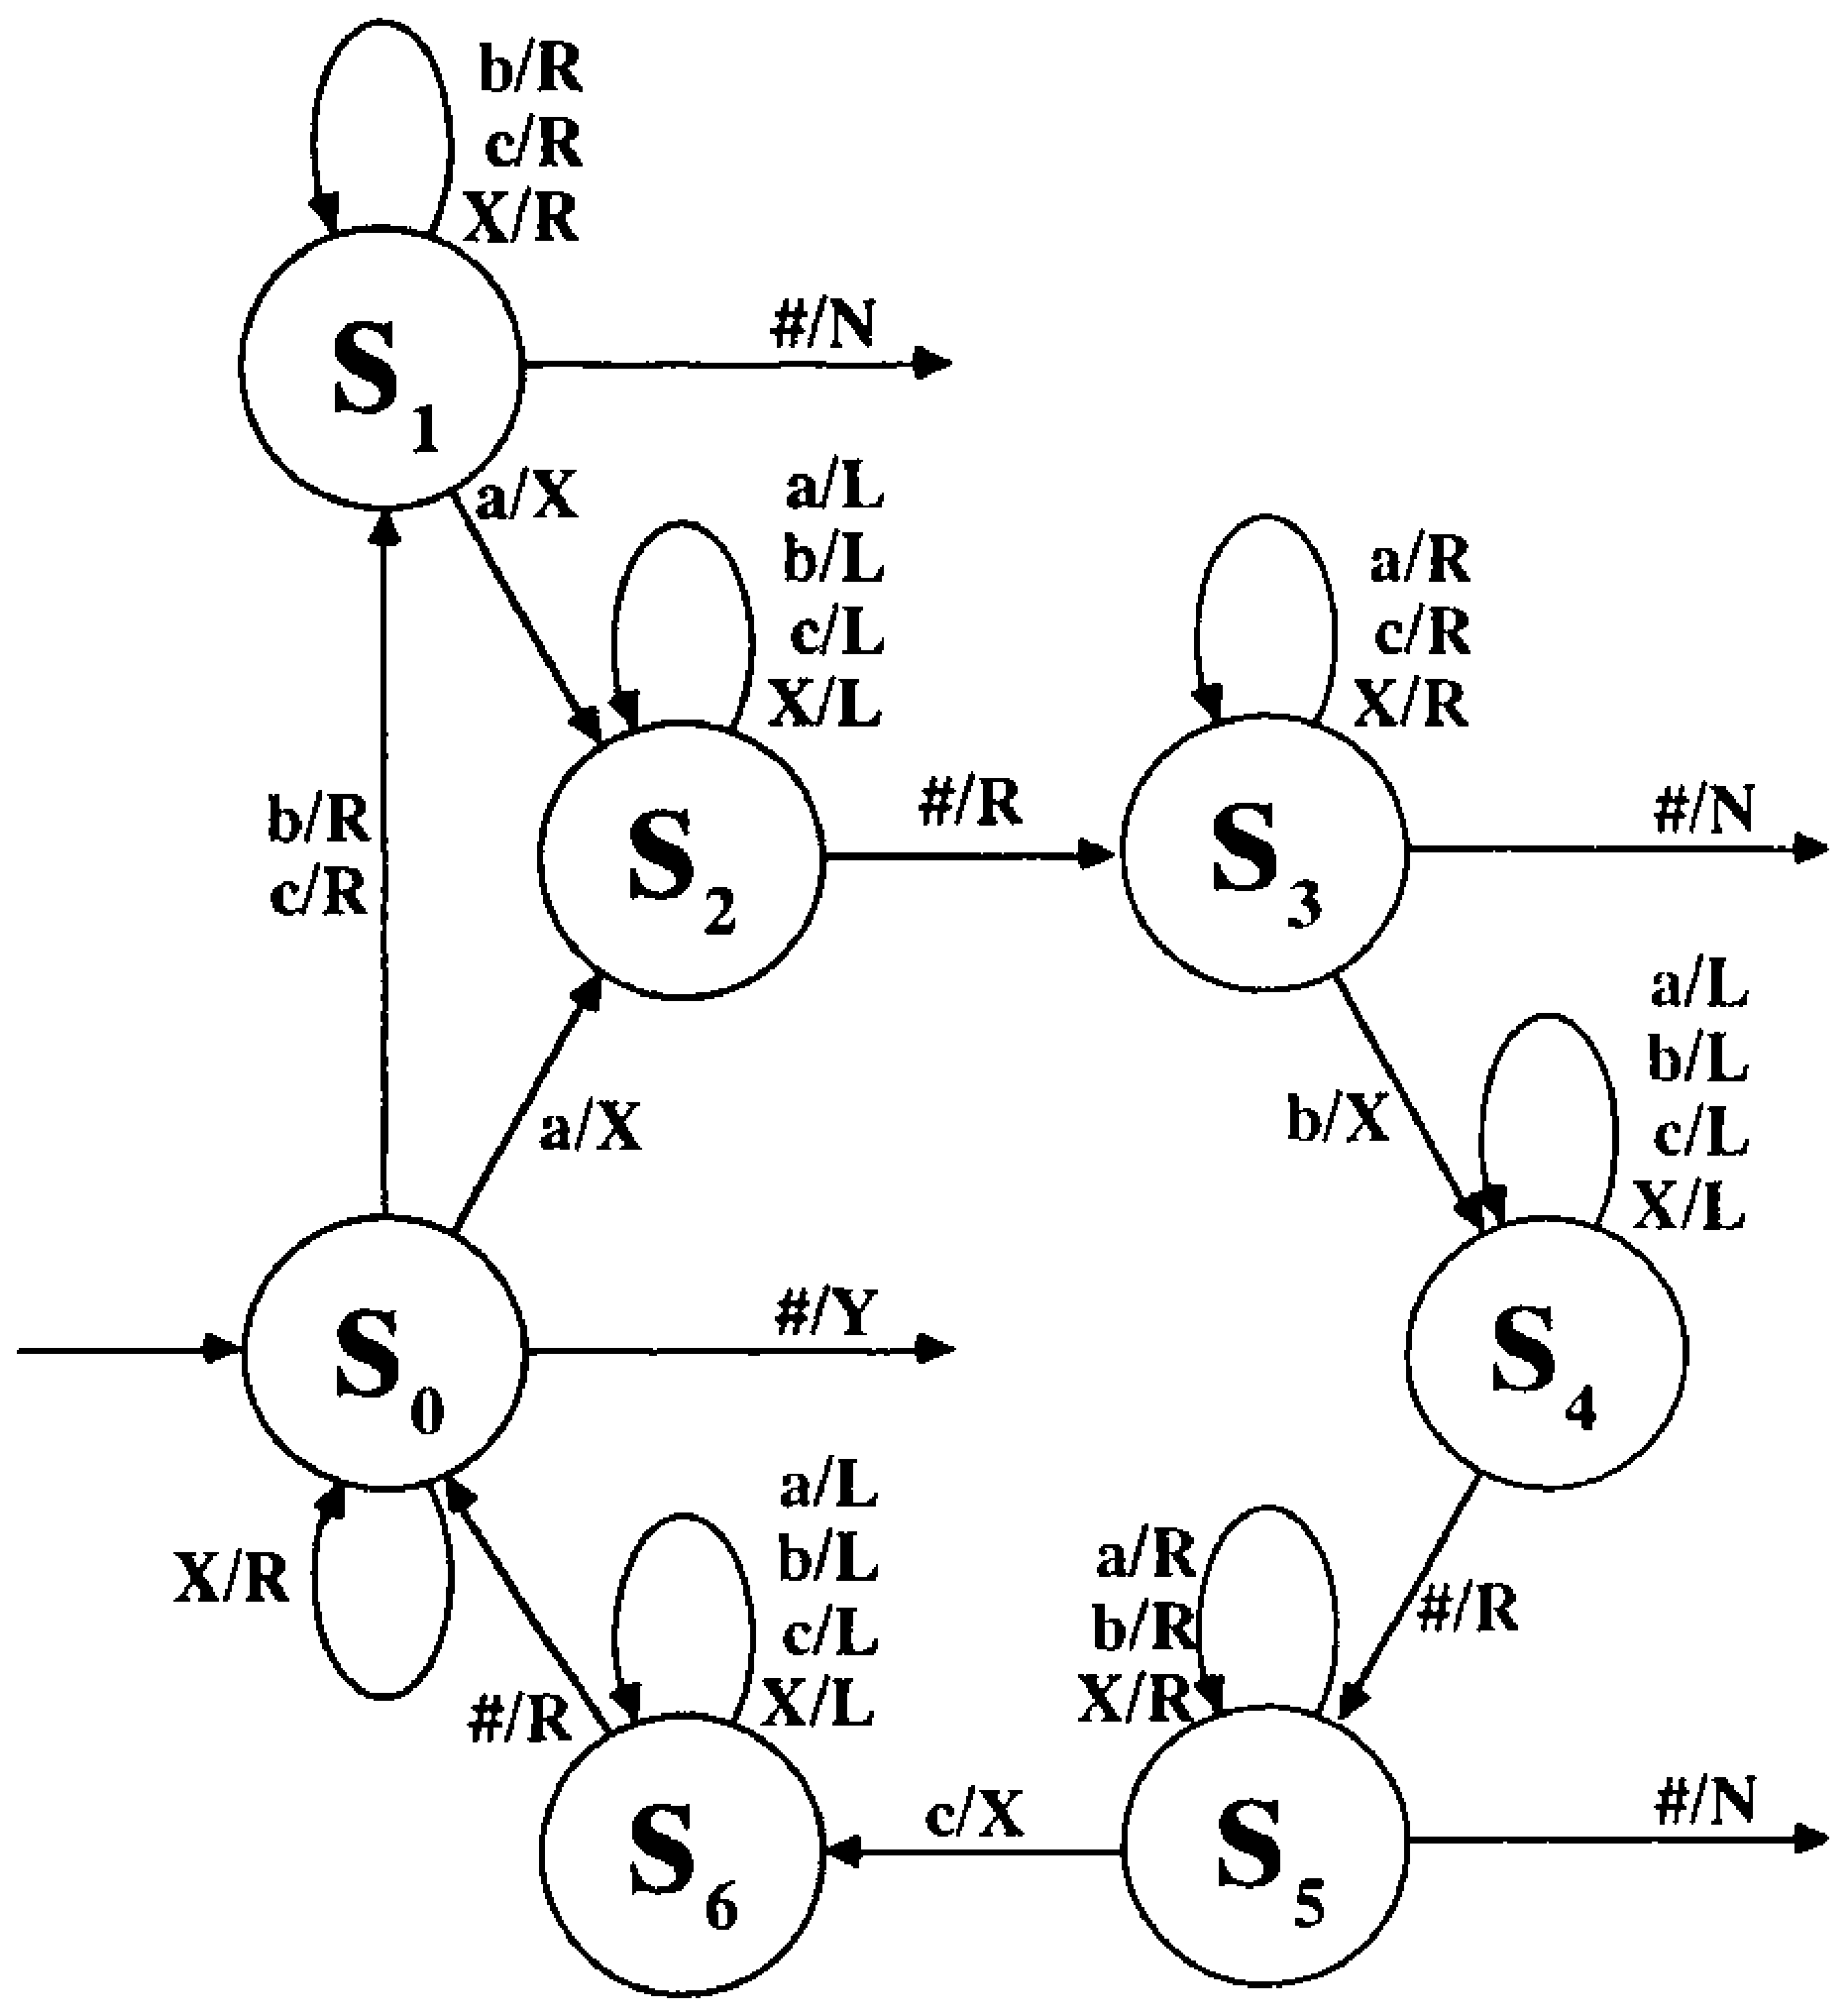
\epsfig{figure=ToFAfigures/fig11-4.eps,height=3.4in}}
\caption{The Turing machine $M$ discussed in Example 11.2}\label{fig-11.4}
\end{figure}

To see exactly how the machine operates, it is useful to step through the
computation for an input string such as $\pmb{babcca}$. To do this, conventions
to designate the status of the device are quite helpful. Like the stack in a
PDA, the tape contents may change as transitions occur, and the notation for the
configuration of a Turing machine must reflect those changes. Steps in a
computation will be represented according to the following conventions.

% Definition 11.2
\begin{dfn}\label{dfn-11.2}\index{Turing machine!configuration}
Let $M=\langle\Sigma,\Gamma,S,s_0,\delta\rangle$ be a Turing machine that is
operating on a tape containing\linebreak$\ldots\pmb{\#\#\#}\alpha\pmb{b}\beta\pmb{\#\#\#}\ldots$,
currently in state $t$ with the tape head scanning the $\pmb{b}$, where $\alpha,
\beta\in(\Sigma\cup\Gamma)^*$, $\alpha$ contains no leading blanks and $\beta$
has no trailing blanks. This configuration will be represented by $\alpha t
\pmb{b}\beta$.

$\gamma\vdash\psi$ will be taken to mean that the configuration denoted by
$\psi$ is reached in one transition from $\gamma$. The symbol $\Dvdash$ will
denote the reflexive and transitive closure of \ $\vdash$.
\end{dfn}

That is, the symbol representing the state will be embedded within the string,
just to the left of the symbol being scanned. If $\delta(t,\pmb{b})=\langle s,
\pmb{R}\rangle$, then $\alpha t\pmb{b}\beta\vdash\alpha\pmb{b} s\beta$. The
new placement of the state label within the string indicates that the tape
head has indeed moved right one symbol. The condition $S\cap(\Sigma\cup\Gamma)=
\emptyset$ ensures that there is no confusion as to which symbol in the
configuration representation denotes the state. As with PDAs, $\gamma\Dvdash\psi$
means that $\gamma$ produces $\psi$ in zero or more transitions. Note that the
leading and trailing blanks are not represented, but $\alpha$ and $\beta$ may
contain embedded blanks. Indeed, $\pmb{b}$ may be a blank. The representation $\pmb{ac\#
\#\#}t\pmb{\#}$ indicates that the tape head has moved past the word $\pmb{ac}$ and is
scanning the fourth blank to the right of the word ($\alpha=\pmb{ac\#\#\#},
\pmb{b}=\pmb{\#},\beta=\lambda$). At the other extreme, $t\pmb{\#\#ac}$ shows
the tape head two cells to the left of the word ($\alpha=\lambda,\pmb{b}=
\pmb{\#},\beta=\pmb{\#ac}$). A totally blank tape\index{tape!blank} is represented by $t\pmb{\#}$.

% Definition 11.3
\begin{dfn}\label{dfn-11.3}\index{language!Turing-acceptable}
For a Turing machine $M=\langle\Sigma,\Gamma,S,s_0,\delta\rangle$, the
\emph{\Index{language accepted by $M$}}, denoted by $L(M)$, is $L(M)=\{x\in
\Sigma^*|\ s_0 x\Dvdash xh\pmb{Y}\}$. A language accepted by a Turing machine is
called a \emph{\Index{Turing-acceptable}} language.
\end{dfn}

It is generally convenient to assume that the special symbol $\pmb{Y}$ is not
part of the input alphabet. Note that words can be rejected if the machine does
not print a $\pmb{Y}$ \emph{or} if the machine never halts.

Several reasonable definitions of acceptance can be applied to Turing machines.
One of the most common specifies that the language accepted by $M$ is the set
of all words for which $M$ simply halts, irrespective of what the final tape
contents are. It might be expected that this more robust definition of
acceptance might lead to more (or at least different) languages being recognized.
However, this definition turns out to yield a device with the same cognitive
power as specified by Definition \ref{dfn-11.3}, as indicated below. More precisely, let
us define
\[ L_1(A) = \{x\in\Sigma^*|\ \exists\alpha,\beta\in(\Sigma\cup\Gamma)^*\ni s_0 x
	\Dvdash \alpha h\beta\} \]
$L_1(A)$ is thus the set of all words that cause $A$ to halt. Let $L$ be a
language for which $L=L_1(B)$ for some Turing machine $B$. It can be shown that
there exists another Turing machine $C$ that accepts $L$ according to Definition
\ref{dfn-11.3}; that is, $L_1(B)=L(C)$ for some $C$. The converse is also true: any
language of the form $L(M)$ is $L_1(A)$ for some Turing machine $A$. Other
possible definitions of acceptance include
\[ L_2(M) = \{x\in\Sigma^*|\ \exists\alpha,\beta\in(\Sigma\cup\Gamma)^*\ni s_0 x
	\Dvdash \alpha h\pmb{Y}\beta\} \]
and
\[ L_3(M) = \{x\in\Sigma^*|\ \exists\alpha\in(\Sigma\cup\Gamma)^*\ni s_0 x\Dvdash
	\alpha h\pmb{Y}\} \]
These distinguish all words that halt with $\pmb{Y}$ somewhere on the tape and
all words that halt with $\pmb{Y}$ at the end of the tape, respectively.

It should be clear that a Turing machine $A_1$, accepting $L=L_1(A_1)$ has an
equivalent\index{equivalent!Turing machines} Turing machine $A_2$ for which $L=L_2(A_2)$. $A_2$ can be obtained
from $A_1$ by simply adding a new state and changing the transitions to the halt
state so that they now all go to the new state. The new state prints $\pmb{Y}$
wherever the tape head is and then, upon scanning that $\pmb{Y}$, halts.
Similarly, a Turing machine $A_3$ can be obtained from $A_2$ by instead
requiring the new state to scan right until it finds a blank. It would then
print $\pmb{Y}$ and halt, and $L_2(A_2)=L_3(A_3)$. The technique for modifying
such an $A_3$ to obtain $A_4$ for which $L_3(A_3)=L(A_4)$ is discussed in the
next section and illustrated in Example 11.11.

\subsection*{Example 11.3}

Consider again the machine $M$ in Example 11.2 and the input string
$\pmb{babcca}$. By the strict definition of acceptance given in Definition \ref{dfn-11.3},
$L(M)=\{\lambda\}$, since $\lambda$ is the only word that does not get destroyed
by $M$. Using the looser criteria for acceptance yields a more interesting
language. The following steps show that $s_0\pmb{babcca}\Dvdash\pmb{XXXXXX}h
\pmb{Y}$.
\begin{center}\begin{tabular}{rllll}
$s_0\pmb{babcca}$ & $\vdash\pmb{b}s_1\pmb{abcca}$ & $\vdash\pmb{b}s_2\pmb{Xbcca}$
	& $\vdash s_2\pmb{bXbcca}$ & $\vdash$ \\
$s_2\pmb{\#bXbcca}$ & $\vdash s_3\pmb{bXbcca}$ & $\vdash s_4\pmb{XXbcca}$ &
	$\vdash s_4\pmb{\#XXbcca}$ & $\vdash$ \\
$s_5\pmb{XXbcca}$ & $\vdash\pmb{X}s_5\pmb{Xbcca}$ & $\vdash\pmb{XX}s_5\pmb{bcca}$
	& $\vdash\pmb{XXb}s_5\pmb{cca}$ & $\vdash$ \\
$\pmb{XXb}s_6\pmb{Xca}$ & $\vdash\pmb{XX}s_6\pmb{bXca}$ & $\vdash\pmb{X}s_6
	\pmb{XbXca}$ & $\vdash s_6\pmb{XXbXca}$ & $\vdash$ \\
$s_6\pmb{\#XXbXca}$ & $\vdash s_0\pmb{XXbXca}$ & $\vdash\pmb{X}s_0\pmb{XbXca}$
	& $\vdash\pmb{XX}s_0\pmb{bXca}$ & $\vdash$ \\
$\pmb{XXb}s_1\pmb{Xca}$ && $\Dvdash s_2\pmb{\#XXbXcX}$ && $\Dvdash$ \\
$\pmb{XX}s_3\pmb{bXcX}$ && $\Dvdash s_4\pmb{\#XXXXcX}$ && $\Dvdash$ \\
$\pmb{XXXX}s_5\pmb{cX}$ && $\Dvdash s_6\pmb{\#XXXXXX}$ && $\Dvdash$ \\
$\pmb{XXXXXX}s_0$ && $\vdash\pmb{XXXXXX}h\pmb{Y}$
\end{tabular}\end{center}
The string $\pmb{babcca}$ is therefore accepted. $\pmb{ac}$ is rejected since
$s_0\pmb{ac}\Dvdash\pmb{Xc}h\pmb{N}$. Further analysis shows that $L_3(M)$ is
exactly $\{x\in\{\pmb{a},\pmb{b},\pmb{c}\}^*|\ \ |x|_{\pmb{a}}=|x|_{\pmb{b}}=
|x|_{\pmb{c}}\}$. Since the only place $\pmb{Y}$ is printed is at the end of the
word on the tape, $L_3(M) = L_2(M)$. Every word eventually causes $M$ to halt
with either $\pmb{Y}$ or $\pmb{N}$ on the tape, and so $L_1(M)=\Sigma^*$.

\subsection*{Example 11.4}\index{parenthesis checker}\index{Turing machine!parenthesis checker}\index{balanced parentheses language}

The composite Turing machine shown in Figure \ref{fig-11.5a} employs two submachines (Figure \ref{fig-11.5b} and Figure \ref{fig-11.5c})
and is based on the parenthesis checker included as a sample in the Turing's
World software. The machine will search for correctly matched parentheses,
restoring the original string and printing $\pmb{Y}$ if the string is
syntactically correct, and leaving a $\pmb{\$}$ to mark the offending position if the
string has mismatched parentheses. Asterisks are recorded to the left of the
string as left parentheses are found, and these are erased as they are matched
with right parentheses.

Figure \ref{fig-11.5a} shows the main architecture of the Turing machine. The square nodes
represent the submachines illustrated in Figures \ref{fig-11.5b} and \ref{fig-11.5c}. When $s_0$
encounters a left parenthesis, it marks the occurrence with $\pmb{\$}$, and
transfers control to the submachine $S_1$. $S_1$ moves the read head to the left
end of the string, and deposits one $\pmb{^*}$ there. The cells to the left of the
original string serve as a scratch area; the asterisks record the number of
unmatched left parentheses encountered thus far. Submachine $S_1$ then scans
right until the $\pmb{\$}$ is found; it then restores the original left
parenthesis. At this point, no further internal moves can be made in $S_1$, and
the arrow leaving $s_{12}$ indicates that control should be returned to the
parent automaton.

The transition leaving the square $S_1$ node in Figure \ref{fig-11.5a} now applies, and
the tape head moves to the right of the left parenthesis that was just processed
by $S_1$, and control is returned to $s_0$. $s_0$ continues to move right past
the symbols $\pmb{a}$ and $\pmb{b}$, uses $S_1$ to process subsequent left
parenthesis, and transfers control to the submachine $S_2$ whenever a right
parenthesis is encountered.

Submachine $S_2$ attempts to match a right parenthesis with a previous left
parenthesis. As control was passed to $S_2$, the right parenthesis was replaced
by $\pmb{\$}$ so that this spot on the tape can be identified later. The
transitions in state $s_{20}$ move the tape head left until a blank cell is
scanned. If the cell to the right of this blank does not contain an asterisk,
$s_{21}$ has no moves and control is passed back to the parent Turing machine,
which will enter $s_4$ and move right past all the symbols in the word, printing
$\pmb{N}$ as it halts. The absence of the asterisk implies that no previous
matching left parenthesis had been found, so halting with $\pmb{N}$ is the
appropriate action.

If an asterisk had been found, $s_{21}$ would have replaced it with a blank, and
then would have no further moves, and the return arrow would be followed. The
blank that is now under the tape head will cause the parent automaton to pass
control to $s_3$, which will move right to $ \pmb{\$}$, and the $\pmb{\$}$ is
then restored to $\pmb{)}$. Control returns to $s_0$ as the tape head moves past
this parenthesis.

The start state continues checking the remainder of the word in this fashion.
When the end of the word is reached, $s_6$ is used to examine the left end of
the string; remaining asterisks indicate unmatched left parentheses, and will
yield $\pmb{N}$ as the machine halts from $s_8$. If $s_6$ does not encounter
$\pmb{^*}$, the Turing machine halts with $\pmb{Y}$ and accepts the string from
$s_7$.
\setcounter{figure}{0}
\renewcommand{\thefigure}{\arabic{chapter}.5\alph{figure}}
% Figure 11.5a
\begin{figure}
\centerline{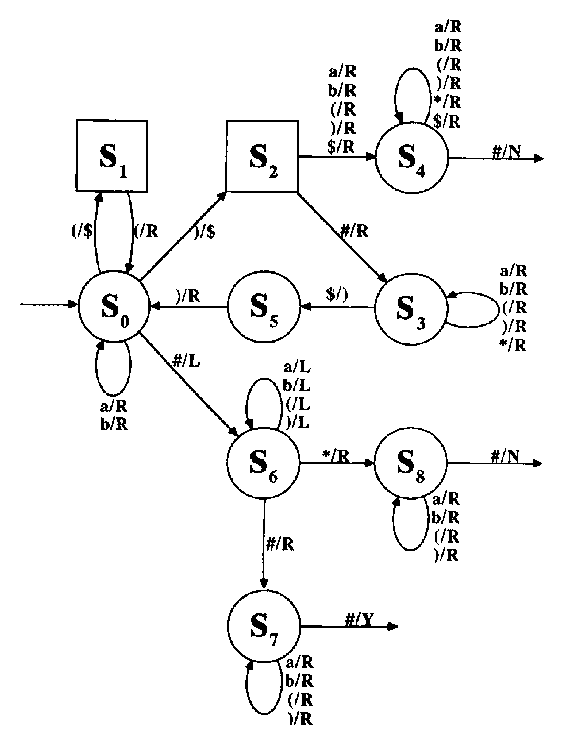
\epsfig{figure=ToFAfigures/fig11-5a.eps,height=4.0in}}
\caption{The Turing machine discussed in Example 11.4}\label{fig-11.5a}
\end{figure}

% Figure 11.5b
\begin{figure}
\centerline{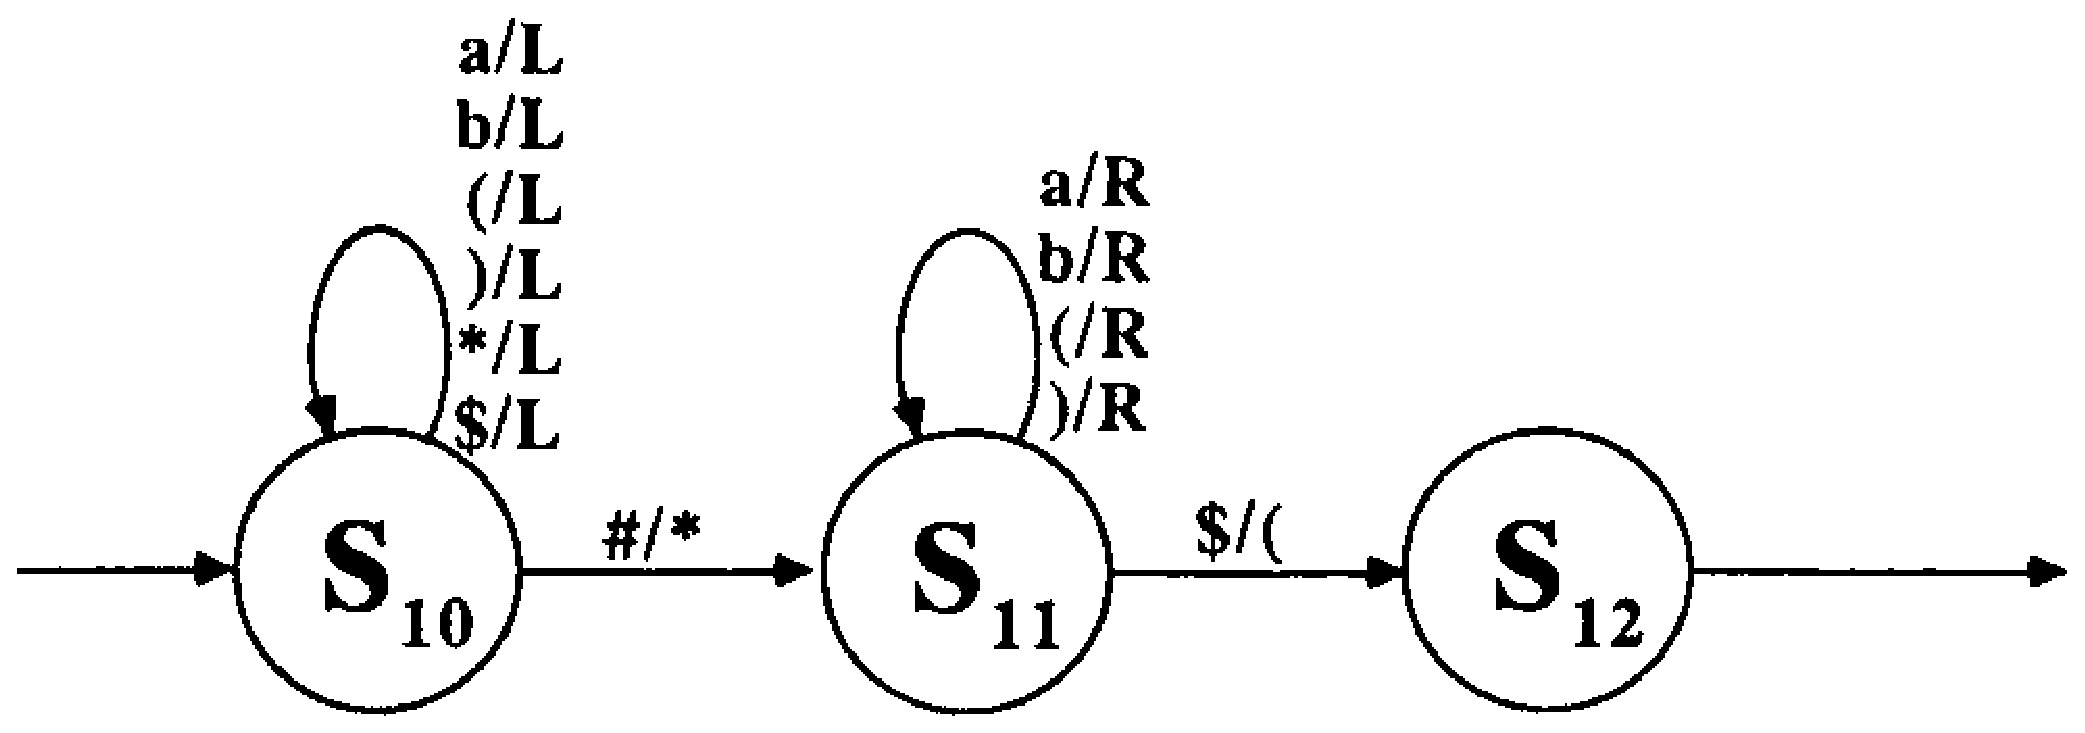
\epsfig{figure=ToFAfigures/fig11-5b.eps,height=1.2in}}
\caption{Submachine $S_1$ in Example 11.4}\label{fig-11.5b}
\end{figure}

% Figure 11.5c
\begin{figure}
\centerline{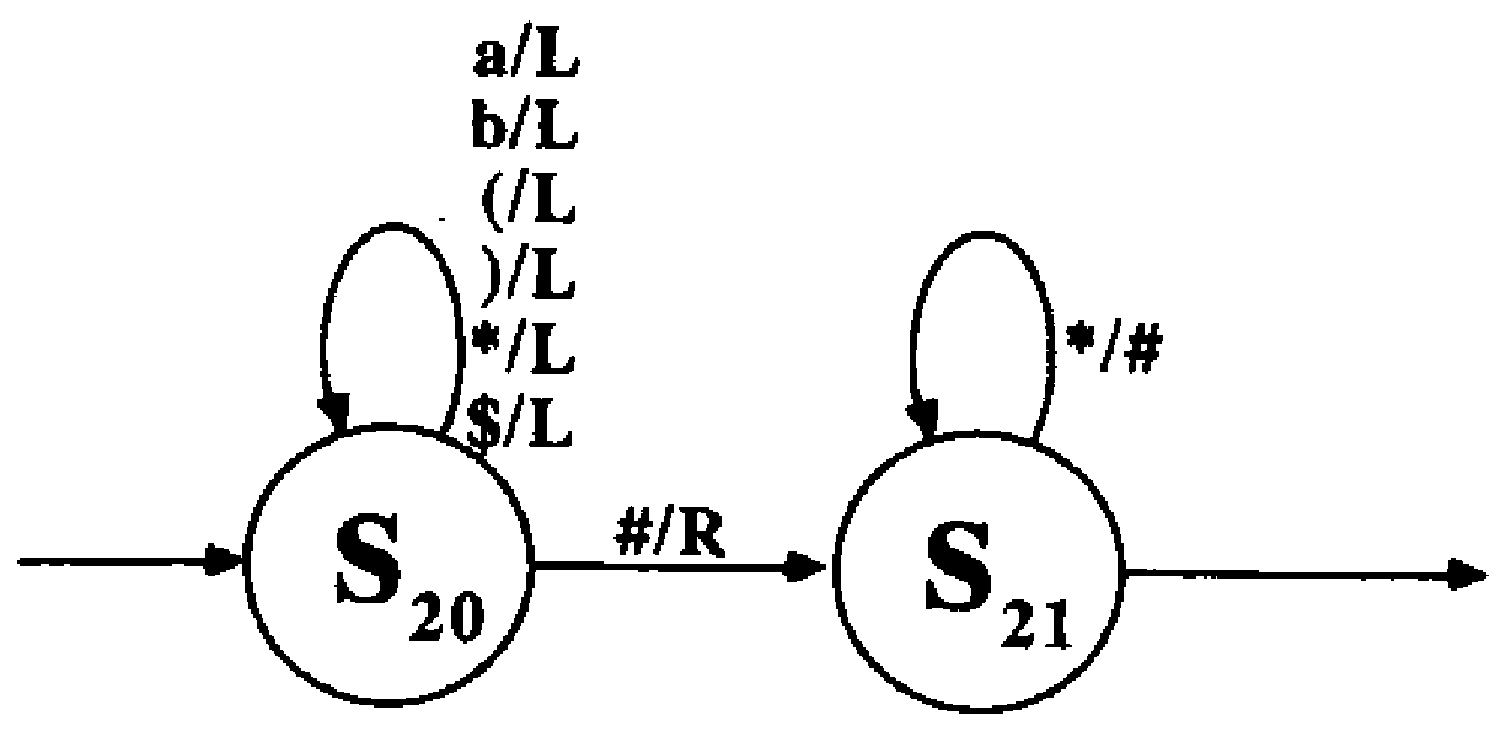
\epsfig{figure=ToFAfigures/fig11-5c.eps,height=1.2in}}
\caption{Submachine $S_2$ in Example 11.4}\label{fig-11.5c}
\end{figure}
\setcounter{figure}{5}                        %nasty kluge
\renewcommand{\thefigure}{\arabic{chapter}.\arabic{figure}}

As more complex examples are considered, one may begin to suspect that any
programming assignment could be carried out on a Turing machine. While it would
be truly unwise to try to make a living selling computers with this architecture,
these devices are generally regarded to be as powerful as any general-purpose
computer. That is, if an algorithm for solving a class of problems can be
carried out on a computer, then there should be a Turing machine that can
produce identical output for each instance of a problem in that class.

The language $\{x\in\{\pmb{a},\pmb{b},\pmb{c}\}^*|\ \ |x|_{\pmb{a}}=|x|_{\pmb{b}}
=|x|_{\pmb{c}}\}$ is not context free, so it cannot be recognized by a PDA.
Turing machines can therefore accept some languages that PDAs cannot, and we
will see that they can recognize every context-free language. We began with DFAs,
which were then extended to the more powerful PDAs, which have now been eclipsed
by the Turing machine construct. Each of these classes of automata has been
substantially more capable than the previous class. If this text were longer,
one might wonder when the next class of superior machines would be introduced.
Barring the application of magic or divine intuition, there does not seem to be
a ``next class.'' That is, any machine that is constrained to operate
algorithmically by a well-defined set of rules appears to have no more computing
power than do Turing machines.

This constraint, ``to behave in an algorithmic fashion,'' is an intuitive notion
without an obvious exact formal expression. Indeed, ``behaving like a Turing
machine'' is generally regarded as the best way to express this notion! A
discussion of how Turing machines came to be viewed in this manner is perhaps in
order. An excellent in-depth treatment of their history can be found in [BARW].

At the beginning of the twentieth century, mathematicians were searching for a
universal algorithm that could be applied to mechanically prove any well-stated
mathematical formula. This naturally focused attention on the manipulation of
symbols. In 1931, G\"odel showed that algorithms of this sort cannot exist. Since
this implied that there were classes of problems that could not have an
algorithmic solution, this then led to attempts to characterize those problems
that could be effectively ``computed.'' In 1936, Turing introduced his formal
device for symbol manipulation and suggested that the definition of an algorithm
be based on the Turing machine. He also outlined the \emph{halting problem}\index{halting problem!for Turing machines}\index{Turing machine!halting problem}
(discussed later), which demonstrated a problem to which no Turing
machine could possibly provide the correct answer in all instances. The search
for a better, perhaps more powerful characterization of what constitutes an
algorithm continued.

While it cannot be proved that it is impossible to find a better formalization
that is truly more powerful, on the basis of the accumulating evidence, no one
believes that a better formulation exists. For one thing, other attempts at
formalization, including grammars, $\lambda$-calculus, $\mu$-recursive
functions, and Post systems, have all turned out to yield exactly the same
computing power as Turing machines. Second, all attempts at ``improving'' the
capabilities of Turing machines have not expanded the class of languages that
can be recognized. Some of these possible improvements will be examined in the
next section. We close this section by formalizing what Example 11.1 probably
made clear: every DFA can be simulated by a Turing machine.

% Theorem 11.1
\begin{thm}\label{thm-11.1}\index{equivalent!Turing machines}
Every FAD language is Turing acceptable.

\emph{Proof.} We show that given any DFA $A=\langle\Sigma,S,s_0,\delta,F
\rangle$, there is a Turing machine $M_A$ that is equivalent to $A$. Define
$M_A=\langle\Sigma,\{\pmb{\#},\pmb{Y},\pmb{N}\},S,s_0,\delta_A\rangle$, where
$\delta_A$ is defined by
\begin{center}\begin{tabular}{r@{ = }l}
$(\forall s\in S)(\forall\pmb{a}\in\Sigma)(\delta_A(s,\pmb{a})$ & $\langle
	\delta(s,\pmb{a}),\pmb{R}\rangle)$ \\
$(\forall s\in F)(\delta_A(s,\pmb{\#})$ & $\langle h,\pmb{Y}\rangle)$ \\
$(\forall s\in S-F)(\delta_A(s,\pmb{\#})$ & $\langle h,\pmb{N}\rangle)$
\end{tabular}\end{center}
A simple inductive argument on $|x|$ shows that
\[ (\forall x\in\Sigma^*)(\forall\alpha,\beta\in(\Sigma\cup\Gamma)^*)(\alpha tx 
	\beta\Dvdash \alpha xq\beta\text{ iff }\DBAR_A(t,x) = q) \]
From this it follows that
\[ (\forall x\in\Sigma^*)(s_0x\Dvdash xq\pmb{\#}\text{ iff }\DBAR_A(s_0,x)=q) \]
Therefore,
\[ (\forall x\in\Sigma^*)(s_0x\Dvdash xh\pmb{Y}\text{ iff }\DBAR_A(s_0,x)\in
	F) \]
which means that $L(M_A)=L(A)$.
\end{thm}

This result actually follows trivially from the much stronger results presented
later. Not only is every type 3 language Turing acceptable, but every type 0
language is Turing acceptable (as will be shown by Theorem \ref{thm-11.2}). The above
proof presents the far more straightforward conversion available to type 3
languages and illustrates the flavor of the inductive arguments needed in other
proofs concerning Turing machines. By using this conversion, the  \Index{Turing's World}$^{\copyright}$
software can be employed to interactively build and test deterministic finite
automata on the Apple$^{\text{\textregistered}}$ Macintosh.

\subsection*{Example 11.5}

Consider the DFA $T$ shown in Figure \ref{fig-11.6}, which recognizes all words of even
length over $\{\pmb{a},\pmb{b}\}$. The corresponding Turing machine is
illustrated in Example 11.1 (see Figure \ref{fig-11.2}).

% Figure 11.6
\begin{figure}
\centerline{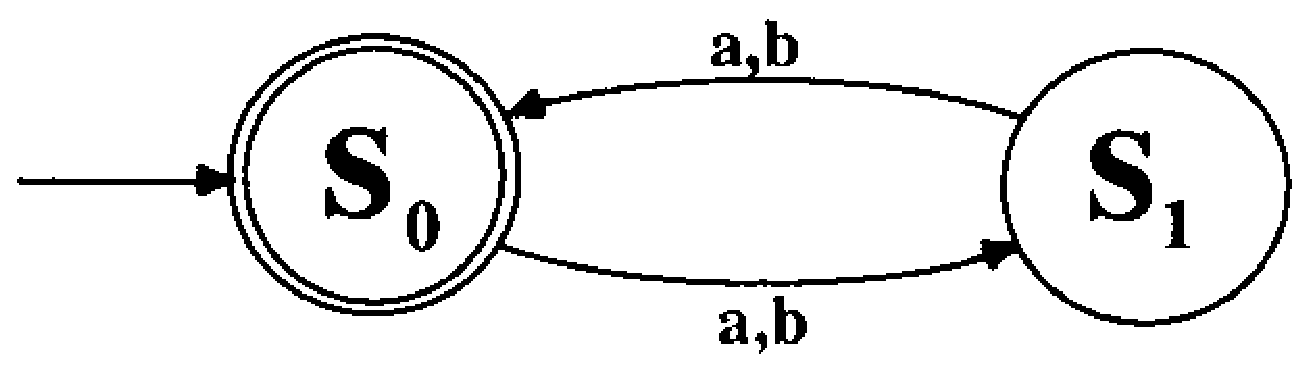
\epsfig{figure=ToFAfigures/fig11-6.eps,width=2.4in}}
\caption{The DFA $T$ discussed in Example 11.5}\label{fig-11.6}
\end{figure}

\section{Variants of Turing Machines}\label{sec-11.2}

There are several ways in which the basic definition of the Turing machine can
be modified. For example, Definition \ref{dfn-11.1} disallows the tape head from both
moving and printing during a single transition. It should be clear that if such
an effect were desired at some point it could be effectively accomplished under
the more restrictive Definition \ref{dfn-11.1} by adding a state to the finite-state
control. The desired symbol could be printed as control is transferred to the
new state. The transition out of the new state would then move the tape head in
the appropriate fashion, thus accomplishing in two steps what a ``fancier''
automaton might do in one step. While this modification might be convenient,
the ability of Definition \ref{dfn-11.1}-style machines to simulate this behavior makes it
clear that such modified automata are no more powerful than those given by
Definition \ref{dfn-11.1}. That is, every such modified automaton has an equivalent Turing
machine.\index{equivalent!Turing machines}

It is also possible to examine machines that are more restrictive than
Definition \ref{dfn-11.1}. If the machine were constrained to write on only a fixed,
finite amount of the tape, this would seriously limit the types of languages
that could be recognized. In fact, only the type 3 languages can be accepted by
such machines.  \emph{Linear bounded automata}, \index{linear bounded automaton} which are Turing machines
constrained to write only on the portion of the tape containing the original
input word, are also less powerful than unrestricted Turing machines and are
discussed in a later section. Having an unbounded area in which to write is
therefore an important factor in the cognitive power of Turing machines, but it
can be shown that the tape need not be unbounded in both directions.\index{Turing machine!bounded on one end} That is,
Turing machines that cannot move left of the cell the tape head originally
scanned can perform any calculation that can be carried out by the
less-restrictive machines given by Definition \ref{dfn-11.1} (see the exercises).

In deciding whether a Turing machine can simulate the modified machines
suggested below, it is important to remember that the auxiliary alphabet
$\Gamma$ can be expanded as necessary, as long as it remains finite. In
particular, it is possible to expand the information content of each cell by
adding a second ``track'' to the tape. For example, we may wish to add check
marks to certain designated cells, as shown in Figure \ref{fig-11.7}. The lower track
would contain the original symbols, and the upper track mayor may not have a
check mark. This can be accomplished by doubling the combined size of the
alphabets $\Sigma$ and $\Gamma$ to include all symbols without check marks and
the same symbols with check marks. The new symbols can be thought of as ordered
pairs, and erasing a check mark then amounts to rewriting a pair such as
$\langle\pmb{a},\sqrt{}\rangle$ with $\langle\pmb{a},\pmb{\#}\rangle$. A scheme
such as this could be used to modify the automaton in Example 11.2. Rather than
replacing designated symbols with $\pmb{X}$, a check could instead be placed
over the original symbol. Just prior to acceptance, each check mark could be
erased, leaving the original string to the left of the $\pmb{Y}$ (see Example
11.11).

% Figure 11.7
\begin{figure}\index{multi-track Turing machine}\index{Turing machine!multi-track}
\centerline{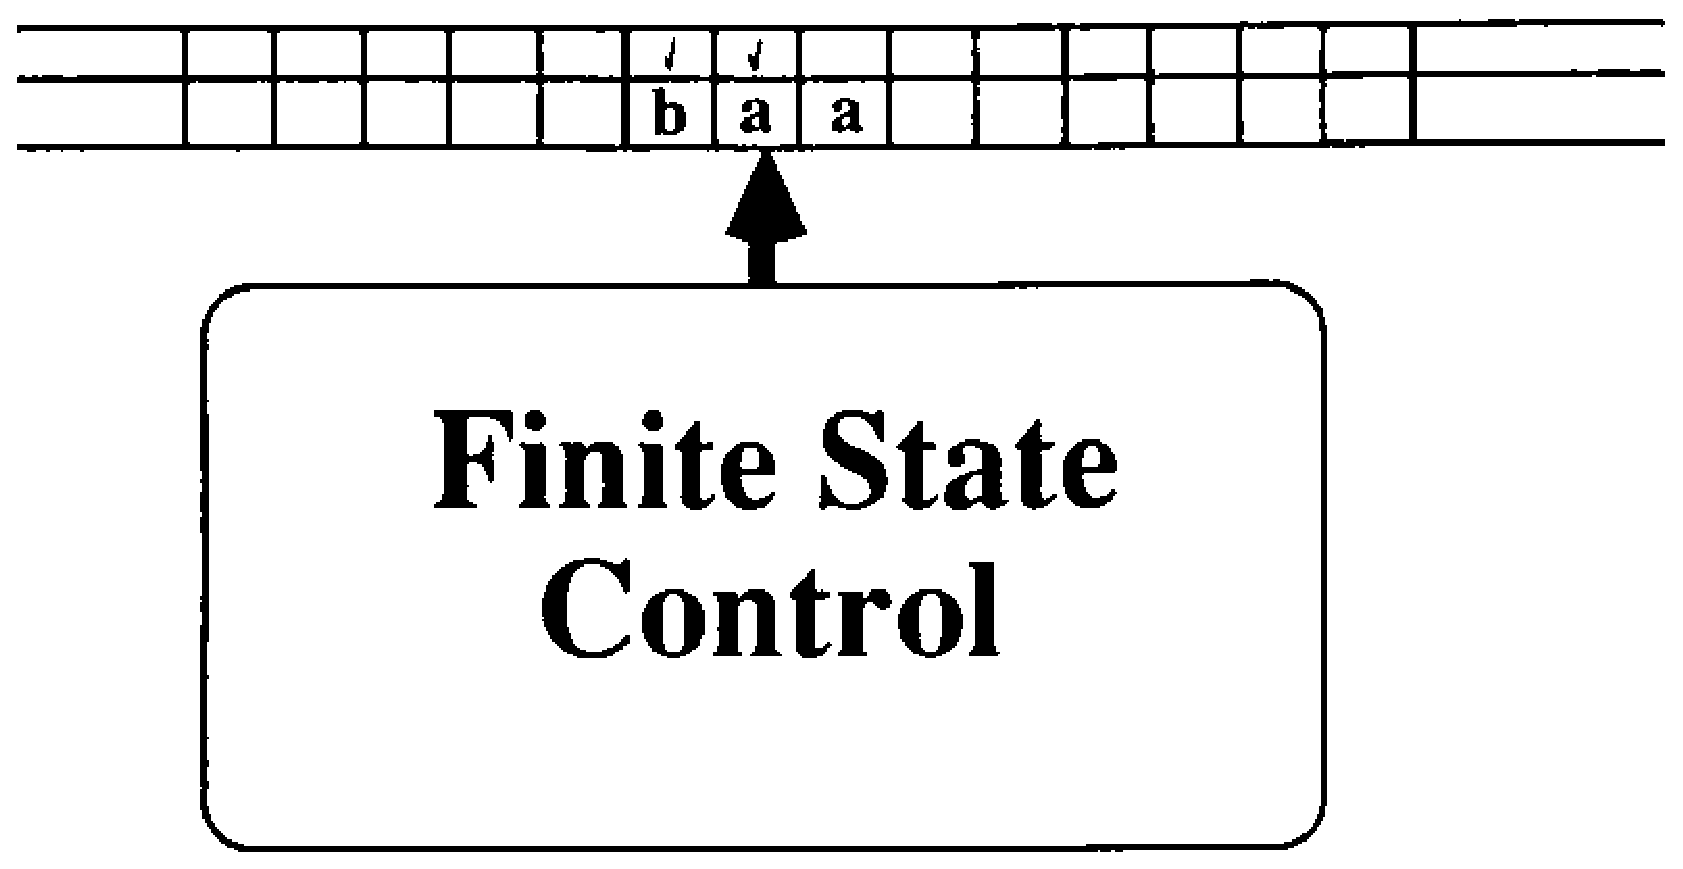
\epsfig{figure=ToFAfigures/fig11-7.eps,width=3.4in}}
\caption{A Turing machine with a two-track tape}\label{fig-11.7}
\end{figure}
 
The foregoing discussion justifies that a Turing machine with a tape head
capable of reading two tracks can be simulated by a Definition \ref{dfn-11.1} style Turing
machine; indeed, it \emph{is} a Turing machine with a slightly more complex alphabet.
When convenient, then, we may assume that we have a Turing machine with two
tracks. A similar argument shows that, for any finite number $k$, a $k$-track
machine has an equivalent\index{equivalent!Turing machines} one-track Turing machine with an expanded alphabet.
The symbols on the other tracks can be more varied than just $\sqrt{}$ and
$\pmb{\#}$; any finite number of symbols may appear on any of the tracks.
Indeed, a Turing machine may initially make a copy of the input string on another
track to use in a later calculation and/or to restore the tape to its original
form. The ability to preserve the input word in this manner illustrates why each
language $L=L_3(A)$ for some Turing machine $A$ must be Turing acceptable; that
is, $L=L_3(A)$ implies that there is a multitrack Turing machine $M$ for which
$L=L(M)$.

\subsection*{Example 11.6}\index{tape!multi-track}

Conceptualizing the tape as being divided into tracks simplifies many of the
arguments concerning modification of the basic Turing machine design. For
example, a modified Turing machine might have two heads that move independently
up and down a single tape, both scanning symbols to determine what transition
should be made and both capable of moving in either direction (or remaining
stationary and overwriting the current cell) as each transition is carried out.
Such machines would be handy for recognizing certain languages. The set
$\{\pmb{a}^n\pmb{b}^n| n\geq 1\}$ can be easily recognized by such a machine.
If both heads started at the left of the word, one head might first scan right
to the first $\pmb{b}$ encountered. The two heads could then begin moving in
unison to the right, comparing symbols as they progressed, until the leading
head encounters a blank and/or the trailing head scans its first $\pmb{b}$. If
these two events occurred on the same move, the word would be accepted. A single
head Turing machine would have to travel back and forth across the word several
times to ascertain if it contained the same number of $\pmb{a}$s as $\pmb{b}$s.
The ease with which the two-headed mutation accomplished the same task might
make one wonder whether such a modified machine can recognize any languages
which the standard Turing machine cannot.

% Figure 11.8
\begin{figure}
\centerline{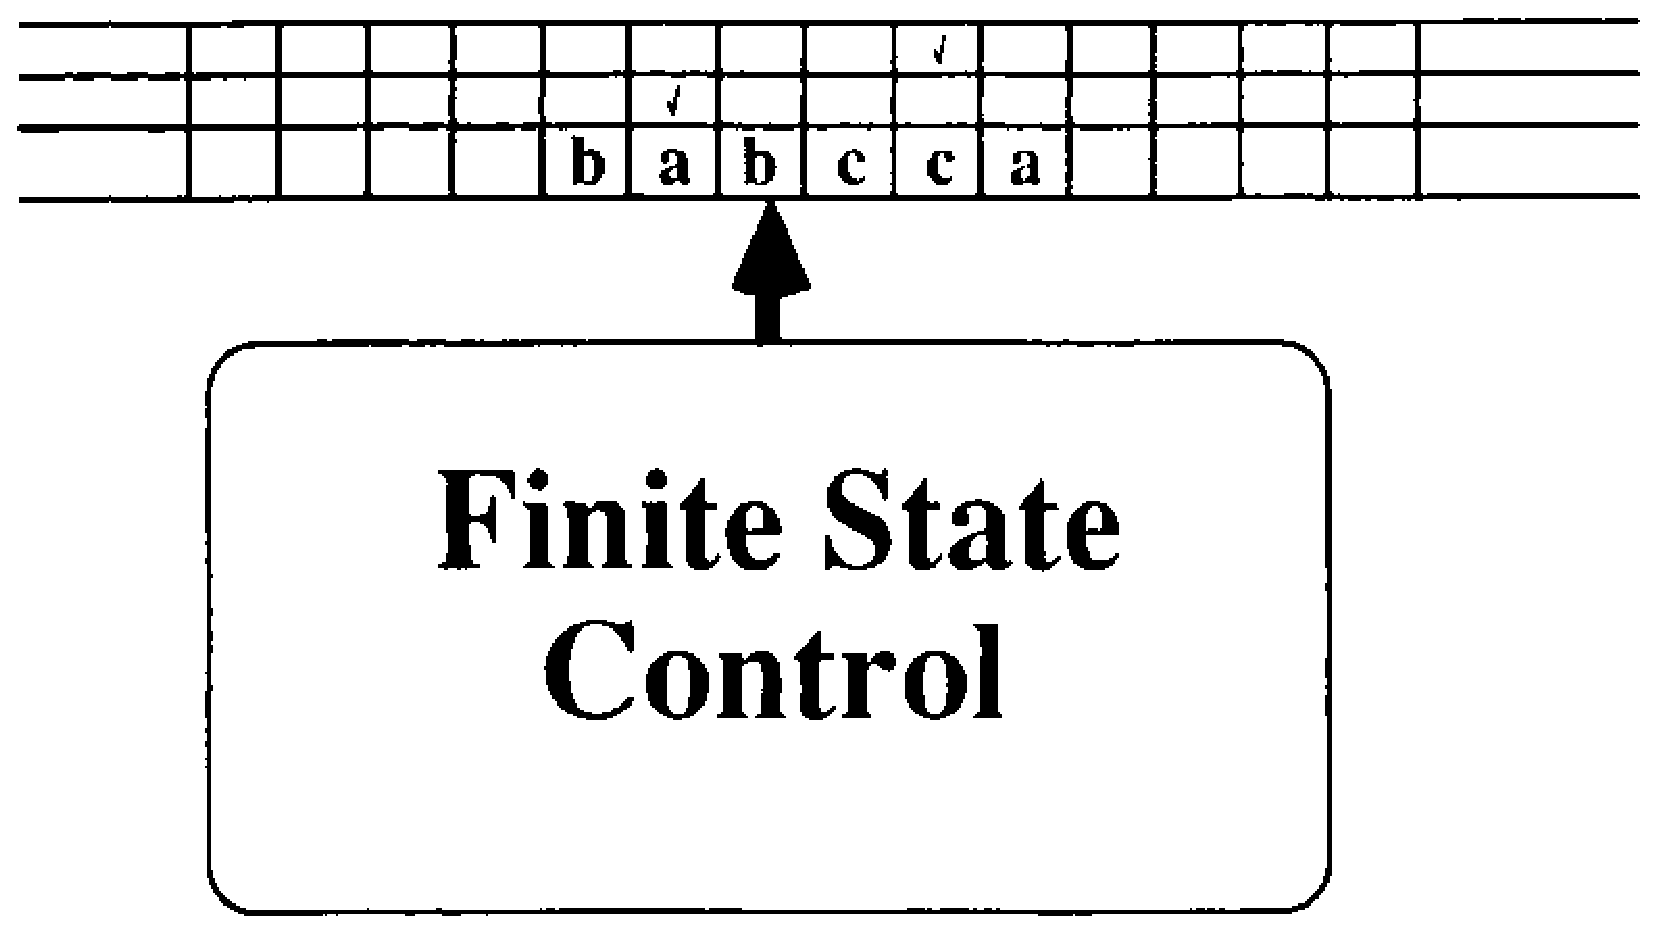
\epsfig{figure=ToFAfigures/fig11-8.eps,width=3.4in}}
\caption{Emulating a two-headed Turing machine with a three-track tape}\label{fig-11.8}
\end{figure}

To justify that a two-headed Turing machine is no more powerful than the type
described by Definition \ref{dfn-11.1}, we must show that any two-headed machine can be
simulated by a corresponding standard Turing machine. As suggested by Figure
\ref{fig-11.8}, a three-track Turing machine will suffice. The original information would
remain on the first track, and check marks will be placed on tracks 2 and 3 to
signify the simulated locations of the two heads. Several moves of the single
head will be necessary to simulate just one move of the two-headed variant, and
the finite-state control must be replicated and augmented to keep track of the
stages of the computation. Each simulated move will begin with the single tape
head positioned over the leftmost check mark. The tape contents are scanned, and
the symbol found is remembered by the finite state control. The tape head then
moves right until the second check mark is found. At this point, the device will
have available the input symbols that would have been scanned by both heads in
the two-headed variant, and hence it can determine what action each of the heads
would have taken. The rightmost checkmark would then be moved left or right or
the current symbol on track 1 overwritten, whichever is appropriate. The single
tape head would then scan left until the other check mark is found, which would
then be similarly updated. This would complete the simulation of one move, and
the process would then repeat.

Various special cases must be dealt with carefully, such as when both heads
would be scanning the same symbol and when the heads ``cross'' to leave a
different head as the leftmost. These cases are tedious but straightforward to
sort out, and thus any language that can be recognized by a two-headed machine
can be recognized by a standard Turing machine. Similarly, a $k$-headed Turing
machine can be simulated by a machine conforming to Definition \ref{dfn-11.1}. The number
of tracks required would then be $k+1$, and the set of states must expand so
that the device can count the number of check marks scanned on the left and
right sweeps of the tape.

Multihead Turing machines are therefore fundamentally no more powerful than the
single-head variety. This means that whenever we need to justify that some task
can be accomplished by a Turing machine we may employ a variant with several
heads whenever this is convenient. We have seen that this variant simplified the
justification that $\{\pmb{a}^n\pmb{b}^n|n\geq 1\}$ was Turing acceptable. It
can also be useful in showing that other variants are no more powerful than the
type of machines given by Definition \ref{dfn-11.1}, as illustrated in the next example.

\subsection*{Example 11.7}

Consider now a device employing several independent tapes with one head for each
tape, as depicted in Figure \ref{fig-11.9}. If we think of the tapes as stationary and the
heads mobile, it is easy to see that we could simply glue the tapes together
into one thick tape with several tracks, as indicated in Figure \ref{fig-11.10}. The
multiple heads would now scan an entire column of cells, but a head would
ignore the information on all but the track for which it was responsible. In
this fashion, a multitape Turing machine can be simulated by a multihead Turing
machine, which can in turn be simulated by a standard Turing machine. Thus,
multitape machines are no more powerful than the machines considered earlier.

% Figure 11.9
\begin{figure}\index{multi-head Turing machine}\index{Turing machine!multi-head}
\centerline{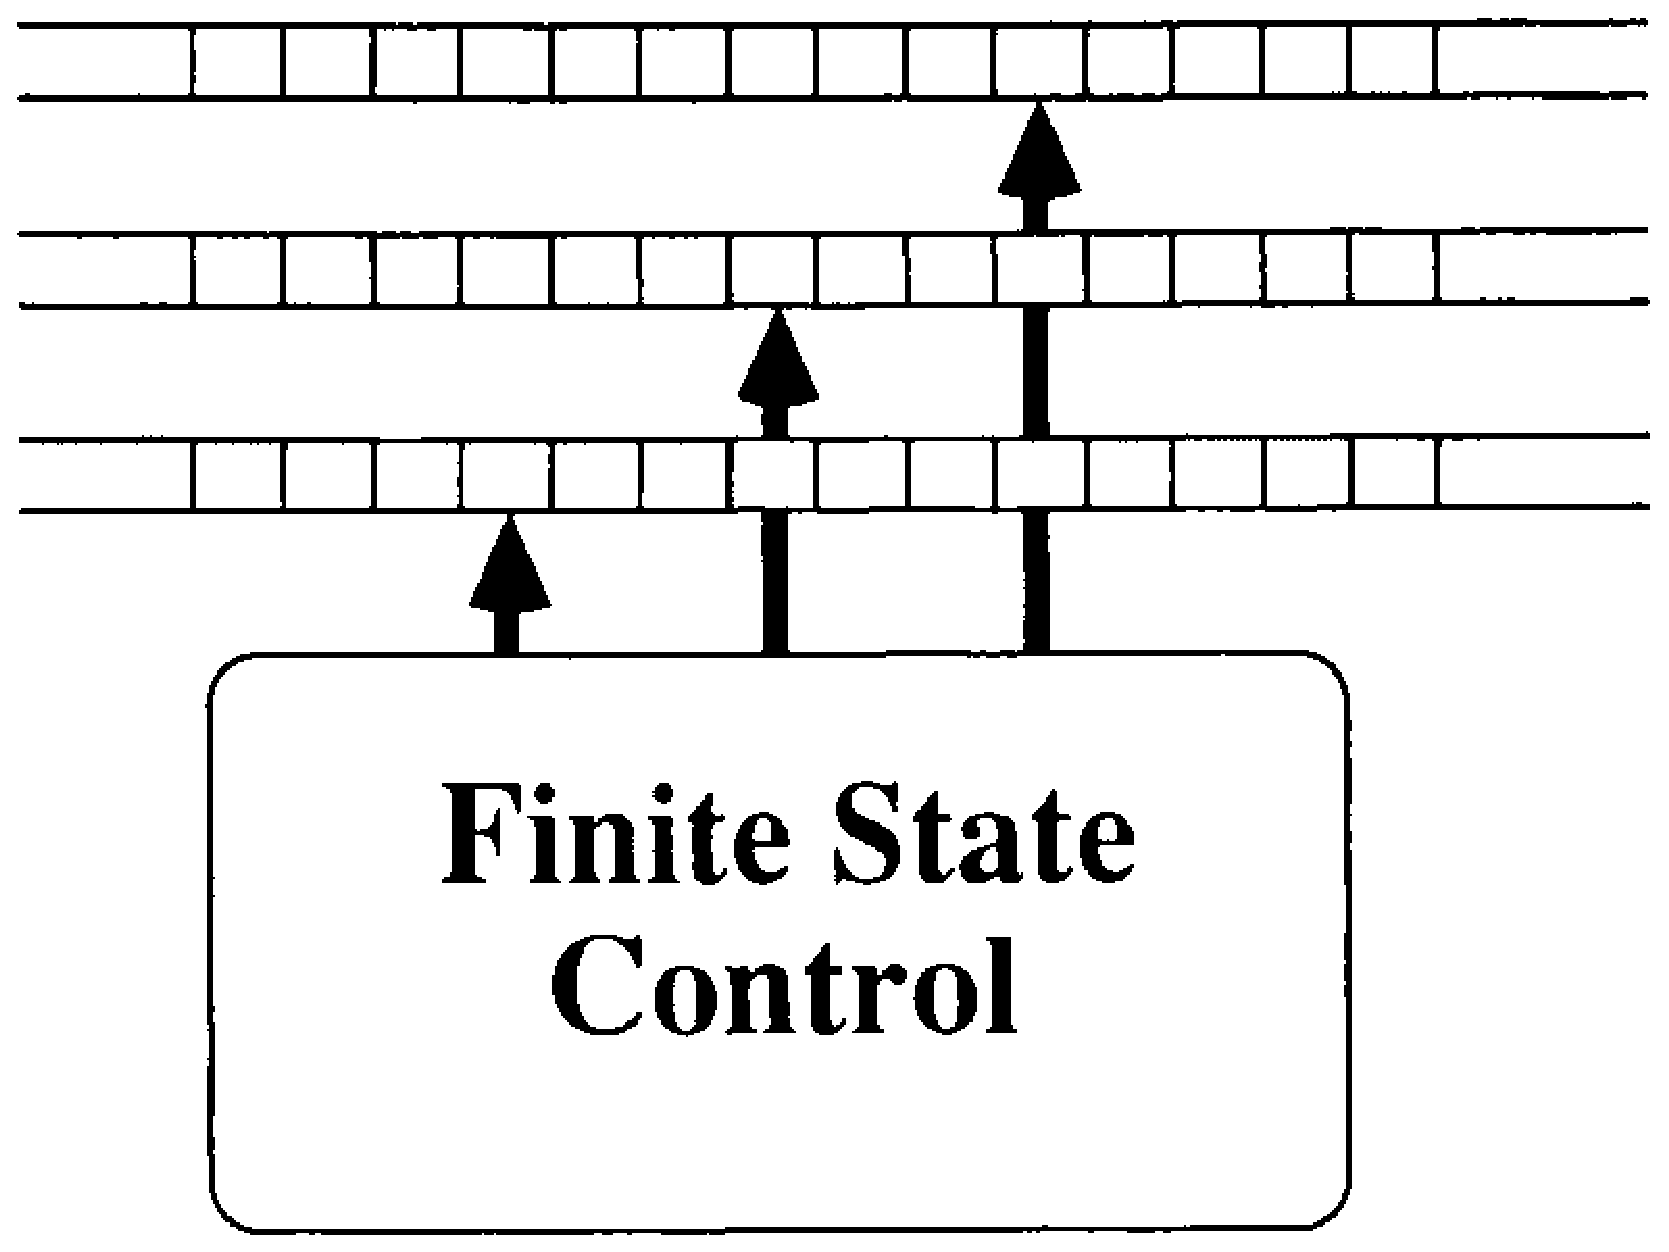
\epsfig{figure=ToFAfigures/fig11-9.eps,width=3.4in}}
\caption{A three-tape Turing machine}\label{fig-11.9}
\end{figure}

% Figure 11.10
\begin{figure}
\centerline{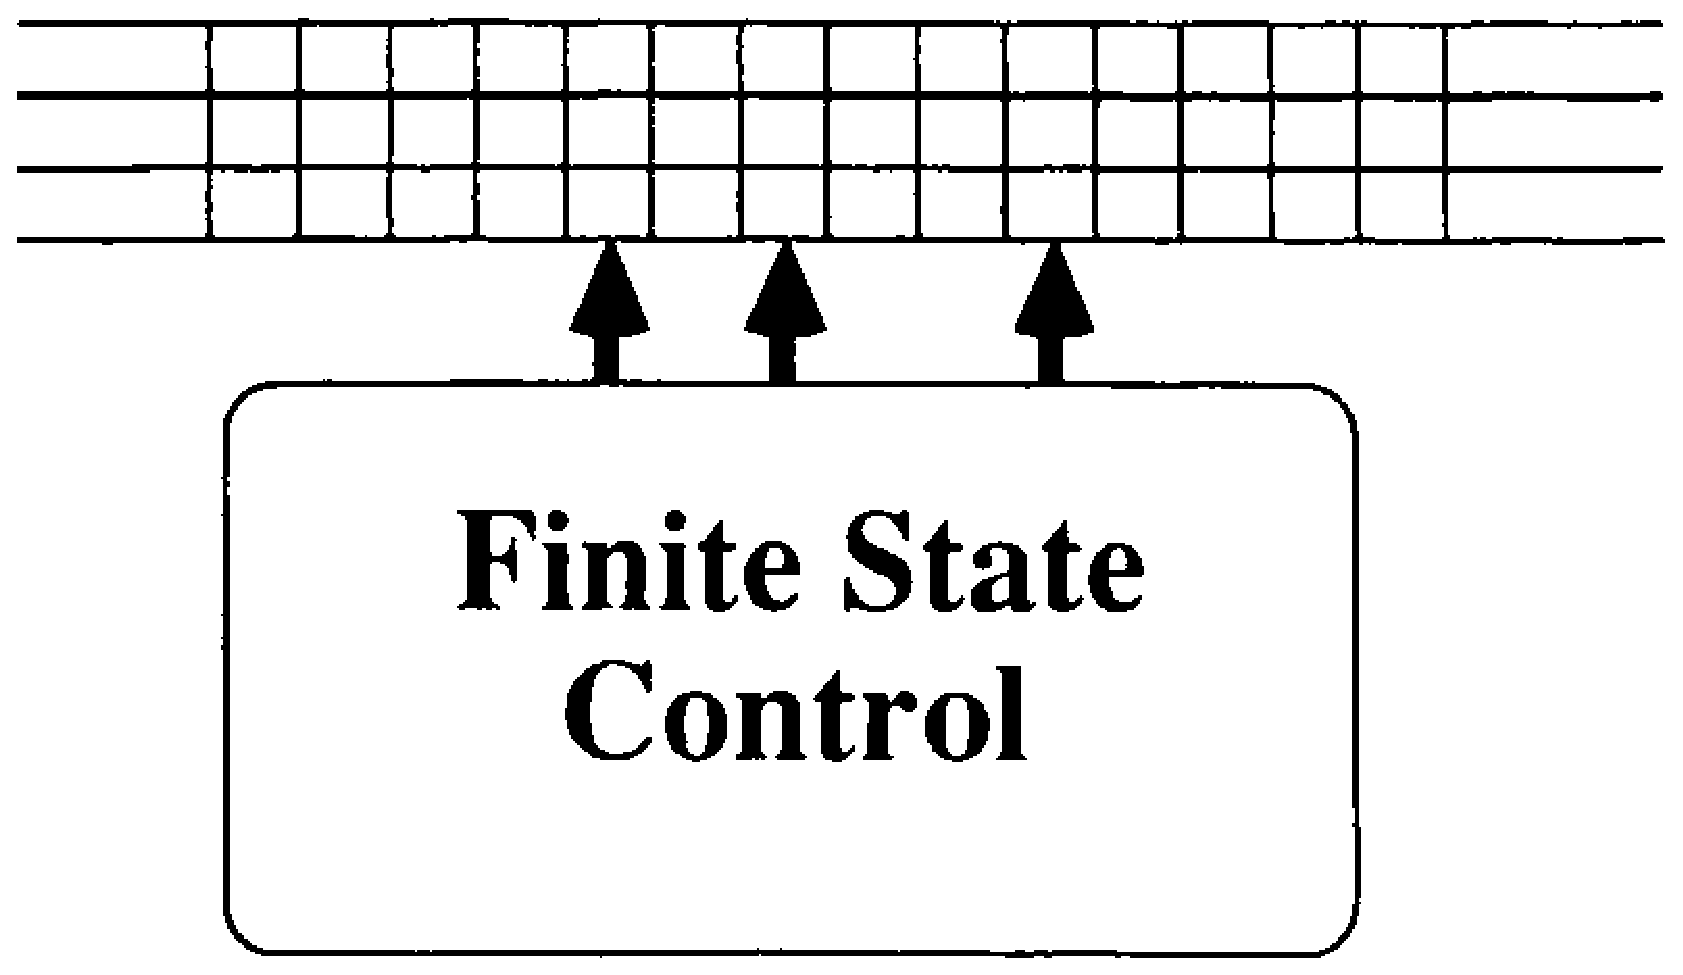
\epsfig{figure=ToFAfigures/fig11-10.eps,width=3.4in}}
\caption{Emulating a three-tape Turing machine with a single three-track tape}\label{fig-11.10}
\end{figure}

One of the wilder enhancements involves the use of a two-dimensional tape, which\index{Turing machine!two-dimensional}
would actually be a surface on which the tape head can move not only left and
right, but also up and down to adjacent squares. With some frantic movement of
the tape head on a one-dimensional tape, two-dimensional Turing machines can be
successfully simulated. Indeed, $k$-dimensional machines (for finite $k$) are no
more powerful than a standard Turing machine. The interested reader is referred
to [HOPC].

\subsection*{Example 11.8}
\index{Turing machine!nondeterministic}
\index{nondeterministic Turing machine}
A potentially more interesting question involves the effects that nondeterminism
might have on the computational power of a Turing machine. With finite automata,
it was seen that NDFAs recognized exactly the same class of languages as DFAs.
However, deterministic pushdown automata accepted a distinctly smaller class of
languages than their nondeterministic cousins. It is consequently hard to
develop even an intuition for what ``should'' happen when nondeterminism is
introduced to the Turing machine construct.

Before we can address this question, we must first define what we mean by a
nondeterministic Turing machine. As with finite automata and pushdown automata,
we may wish to allow a choice of moves from a given configuration, leading to
several disparate sequences of moves for a given input string. Like NDFAs and
NPDAs, we will consider a word accepted if there is at least one sequence of
moves that would have resulted in a $\pmb{Y}$ being printed. Simulating such
machines with deterministic Turing machines is more involved than it may at
first seem. If each possible computation was guaranteed to halt, it would be
reasonable to try each sequence of moves, one after the other, halting only when
a $\pmb{Y}$ was found. If one sequence led to an $\pmb{N}$ being printed, we
would then move on to the next candidate. Since there may be a countable number
of sequences to try, this process may never end. This is not really a problem,
since if a sequence resulting in a $\pmb{Y}$ exists, it will eventually be found
and tried, and the machine will halt and accept the word. If no such sequence
resulting in a $\pmb{Y}$ exists, and there are an infinite number of negative
attempts to be checked, the machine will never halt. By our original definition
of acceptance, this will result in the word being rejected, which is the desired
result.

The trouble arises in trying to simulate machines that are not guaranteed to
halt under all possible circumstances. This is not an inconsequential concern;
in Chapter \ref{ch-12}, we will identify some languages that are so complex that their
corresponding Turing machines cannot halt for all input strings. A problem then
arises in trying to switch from one sequence to the next. If, say, the first
sequence we tried did not halt and instead simply continued operation without
ever producing $\pmb{Y}$ or $\pmb{N}$, we would never get the chance to try
other possible move sequences. Since the machine will not halt, the word will
therefore be rejected, even if some later sequence would have produced
$\pmb{Y}$. Simulating the nondeterministic machine in this manner will not be
guaranteed to recognize the same language, and an alternative method must be
used.

This problem is avoided by simulating the various computations in the following
(very inefficient) manner. We begin by simulating the first move of the first
sequence. We then start over with the first move of the second sequence, and
then begin again and simulate two moves in the first sequence. On the next pass,
we simulate the first move of the third sequence, then two moves of the second
sequence, and then three moves of the first sequence. On each pass, we start
computing a new sequence and move a little further along on the sequences that
have already been started. If any of these sequences results in $\pmb{Y}$, we
will eventually simulate enough of that sequence to discover that fact and
accept the word. In this way, we avoid getting trapped in a dead end with no
opportunity to pursue the alternatives.

Implementing the above scheme will produce a deterministic Turing machine that
is equivalent\index{equivalent!Turing machines} to the original nondeterministic machine. It remains to be shown
that the Turing machine can indeed \emph{start over} as necessary, and that the
possible move sequences can be enumerated in a reasonable fashion so that they
can be pursued according to the pattern outlined above. A three-tape
(deterministic) Turing machine will suffice. The first tape will keep an
inviolate copy of the input string, which will be copied onto the second tape
each time a computation begins anew. A specific sequence of steps will be
carried out on this second scratch tape, after which the presence/absence of $\pmb{Y}$
will be determined. The third tape is responsible for keeping track of the
iterations and generating the appropriate sequences to be employed. Enumerating
the sequences is much like the problem of generating words over some alphabet in
lexicographic order (see the exercises). Methods for generating the ``directing
sequences'' can be found in both [LEWI] and [HOPC]. These references also
propose a more efficient approach to the whole simulation, which is based on
keeping track of the sets of possible configurations, much as was done in
%Theorem \ref{thm-4.5} for nondeterministic finite automata.
% NOTE: Theorem 4.5 does NOT exist
Definition \ref{dfn-4.5} for nondeterministic finite automata.

Thus, neither nondeterminism nor any of the enhancements considered above
improved the computational power of these devices. As mentioned previously, no
one has yet been able to find any mechanical enhancement that does yield a
device that can recognize a language that is not Turing acceptable. Attempts at
producing completely different formal systems have fared no better, and there is
little cause to believe that such systems exist. We now turn to characterizing
what appears to be the largest class of algorithmically definable languages. In
the next section, we will see that the Turing-acceptable languages are exactly
the type 0 languages introduced in Chapter \ref{ch-8}.

% Definition 11.4
\begin{dfn}\label{dfn-11.4}\index{T@\TSIG \ (T-sigma )}\index{Z@\ZSIG \ (Z-sigma )}
For a given alphabet $\Sigma$, let \TSIG\ be the collection of all
Turing-acceptable languages, and let \ZSIG\ be the collection of all type 0
languages.
\end{dfn}

The freedom to use several tapes and nondeterminism makes it easier to explore
the capabilities of Turing machines and relate \TSIG\ to the previous classes of
languages encountered. It is now trivial to justify that every PDA can be
simulated by a nondeterministic Turing machine with two tapes. The first tape
will hold the input, which will be scanned by the first tape head, which will
only have to move right or, at worst, remain stationary and reprint the same
character it was scanning. The second tape will function as the stack, with
strings pushed or symbols popped in correspondence with what takes place in the
PDA. Since a Turing machine can only print one symbol at a time, some new states
may be needed in the finite-state control to simulate pushing an entire string,
but the translation process is quite direct.

% Lemma 11.1
\begin{lmm}\label{lmm-11.1}
Let $\Sigma$ be an alphabet. Then $\PSIG\subset\TSIG$. That is, every
context-free language is Turing acceptable, and the containment is proper.

\emph{Proof.} Containment follows from the formalization of the above discussion
(see the exercises). Example 11.3 presented a language over $\{\pmb{a},\pmb{b},
\pmb{c}\}$ that is Turing acceptable but not context free. While the distinction
between \DSIG, and \PSIG, disappeared for singleton alphabets, proper
containment remains between $\mathfrak{P}_{\{\pmb{a}\}}$ and $\mathfrak{T}_{\{
\pmb{a}\}}$, as shown by languages such as $\{\pmb{a}^n|\ n$ is a perfect square
$\}$.
\end{lmm}

In the next section, an even stronger result is discussed, which shows that the
class of Turing-acceptable languages includes much more than just the
context-free languages. Lemma \ref{lmm-11.1} is actually an immediate corollary of Theorem
\ref{thm-11.2}. The next section also explores the formal relationship between Turing
machines and context-sensitive languages.

\section{Turing Machines, LBAs, and Grammars}\label{sec-11.3}

The previous sections have shown that the class of Turing-acceptable languages
properly contains the type 2 languages. We now explore how the type 0 and type
1 languages relate to Turing machines. Since the preceding discussions mentioned
that no formal systems have been found that surpass Turing machines, one would
expect that every language generated by a grammar can be recognized by a Turing
machine. This is indeed the case, as indicated by the following theorem.

% Theorem 11.2
\begin{thm}\label{thm-11.2}\index{equivalent!Turing machines}
Let $\Sigma$ be an alphabet. Then $\ZSIG\subseteq\TSIG$. That is, every type 0
language is Turing acceptable.

\emph{Proof.} We justify that, given any type 0 grammar $G=\langle\Sigma,\Gamma,
S,P\rangle$, there must be a Turing machine $T_G$ that is equivalent to $G$. As
with the suggested conversion of a PDA to a Turing machine, $T_G$ will employ
two tapes and nondeterminism. The first tape again holds the input, which will
be compared to the sentential form generated on the second tape. The second tape
begins with only the start symbol on an otherwise blank tape. The finite-state
control is responsible for nondeterministically guessing the proper sequence of
productions to apply, and with each guess, the second tape is modified to
reflect the new sentential form. If at some point the sentential form agrees
with the contents of the first tape, the machine prints $\pmb{Y}$ and halts. A
guess will consist of choosing both an arbitrary position within the current
sentential form and a particular production to attempt to substitute for the
substring beginning at that position. Only words that can be generated by the
grammar will have a sequence of moves that produces $\pmb{Y}$, and no word that
cannot be generated will be accepted. Thus, the new Turing machine is equivalent
to $G$.
\end{thm}

\subsection*{Example 11.9}

Consider the context-sensitive grammar $G=\langle\{\pmb{a},\pmb{b},\pmb{c}\},\{
S,A,B,C\},S,P\rangle$, where $P$ contains the productions
\begin{enumerate}
\item $Z\rightarrow\lambda$
\vspace{-0.1in}
\item $Z\rightarrow S$
\vspace{-0.1in}
\item $S\rightarrow SABC$
\vspace{-0.1in}
\item $S\rightarrow ABC$
\vspace{-0.1in}
\item $AB\rightarrow BA$
\vspace{-0.1in}
\item $BA\rightarrow AB$
\vspace{-0.1in}
\item $CB\rightarrow BC$
\vspace{-0.1in}
\item $BC\rightarrow CB$
\vspace{-0.1in}
\item $CA\rightarrow AC$
\vspace{-0.1in}
\item $AC\rightarrow CA$
\vspace{-0.1in}
\item $A\rightarrow\pmb{a}$
\vspace{-0.1in}
\item $B\rightarrow\pmb{b}$
\vspace{-0.1in}
\item $C\rightarrow\pmb{c}$
\end{enumerate}
It is quite easy to show that $L(G)=\{x\in\{\pmb{a},\pmb{b},\pmb{c}\}^*|\ \
|x|_{\pmb{a}}=|x|_{\pmb{b}}=|x|_{\pmb{c}}\}$ by observing that no production
changes the relative numbers of (lowercase and capital) $A$s, $B$s, and $C$s,
and the six context-sensitive rules allow them to be arbitrarily reordered. One
of the attempted ``guesses'' made by the Turing machine $T_G$ concerning how the
productions might be applied is:
\begin{quote}
Use (2) beginning at position 1. \\
Use (4) beginning at position 1. \\
Use (6) beginning at position 2. $\ldots$
\end{quote}
This would lead to a failed attempt, since it corresponds to $Z\Rightarrow S
\Rightarrow ABC$, and the substring $BC$ beginning at position 2 does not match
$BA$, the left side of rule 6. On the other hand, there is a pattern of guesses
that would cause the following sequence of symbols to appear on the second tape:
\[ Z\Rightarrow S\Rightarrow ABC\Rightarrow BAC\Rightarrow BCA\Rightarrow
	B\pmb{c}A\Rightarrow B\pmb{ca}\Rightarrow\pmb{bca} \]
This would lead to a favorable comparison if $\pmb{bca}$ was the word on the
input tape. Note that the Turing machine may have to handle shifting over
existing symbols on the scratch tape to accommodate increases in the size of the
sentential form. Since type 0 grammars allow length-reducing productions, the
machine may also be required to shrink the sentential form when a string of
symbols is replaced by a smaller string.

A rather nice feature of type 1 languages is that the length of the sentential
form could never decrease (except perhaps for the application of the initial
production $Z\rightarrow\lambda$), and hence sentential forms that become
longer than the desired word are known to be hopeless. All context-sensitive
(that is, type 1) languages can therefore be recognized by a Turing machine that
use an amount of tape proportional to the length of the input string, as
outlined below.

% Definition 11.5
\begin{dfn}\label{dfn-11.5}\index{alphabet!input}\index{alphabet!auxiliary}
A \emph{\Index{linear bounded automaton}} (\Index{LBA})\index{Turing machine!bounded|see{LBA}}\index{Turing machine!linear bounded|see{LBA}} is a nondeterministic\index{state transition function!for LBA}
Turing machine that recognizes words over an alphabet $\Sigma$ given by the
quintuple $M=\langle\Sigma,\Gamma,S,s_0,\delta\rangle$, where
\begin{quote}
$\Sigma$ is the \emph{input alphabet} \\
$\Gamma$ is the \emph{auxiliary alphabet} containing the special markers $\<$ and\index{end markers for LBA}
	$\>$ and $\Sigma$, $\Gamma$, and $\{\pmb{L},\pmb{R}\}$ are pairwise
	disjoint sets (and thus $\<,\> \notin\Sigma$). \\
$S$ is a finite nonempty set of \emph{states} (and $S\cap(\Sigma\cup\Gamma) =
	\emptyset$). \\
$s_0$ is the \emph{\Index{start state}} ($s_0\in S$). \\
$\delta$ is the \emph{state transition function} $\delta$: $S\times(\Sigma\cup
	\Gamma)\rightarrow(S\cup\{h\}\times(\Sigma\cup\Gamma\cup\{\pmb{L},
	\pmb{R}\})$, where \\
$(\forall s\in S)(\delta(s,\<)=(q,\pmb{R})$ for some $q\in S\cup\{h\})$, and \\
$(\forall s\in S)(\delta(s,\>)=(q,\pmb{L})$ for some $q\in S\cup\{h\}$, or
$\delta(s,\>)=(h,\pmb{Y})$ or $\delta(s,\>)=\langle h,\pmb{N}\rangle)$
\end{quote}
\end{dfn}
That is, the automaton cannot move left of the symbol $\<$ nor overwrite it. The
LBA likewise cannot move right of the symbol $\>$, and it can only overwrite it
with $\pmb{Y}$ or $\pmb{N}$ just prior to halting. The symbols $\#,\pmb{L},\ 
\pmb{R},\ \pmb{Y}$, and $\pmb{N}$ retain their former meaning, although $\#$ can
be dropped from $\Gamma$ since it will never be scanned. As implied by the
following definition, the special markers $\<$ and $\>$ are intended to delimit
the input string, and Definition \ref{dfn-11.5} ensures that the automaton cannot move
past these limits. As has been seen, the use of several tracks can easily
multiply the amount of information that can be stored in a fixed amount of
space, and thus the restriction is essentially that the amount of available tape
is a linear function of the length of the input string. In practice, any Turing
machine variant for which each tape head is constrained to operate within an
area that is a multiple of the length of the input string is called a linear
bounded automaton.

% Definition 11.6
\begin{dfn}\label{dfn-11.6}
For a linear bounded automaton $M=\langle\Sigma,\Gamma,S,s_0,\delta\rangle$, the
\emph{\Index{language accepted by M}}, denoted by $L(M)$, is $L(M)=\{x\in
\Sigma^*|\ \<s_0x\>\Dvdash \<xh\pmb{Y}\}$. A language accepted by a linear bounded
automaton is called a \emph{linear bounded language} (\Index{LBL}).\index{linear bounded language|see{LBL}}\index{language!linear bounded}
\end{dfn}

Note that while the endmarkers must enclose the string $x$, it is the word $x$
(rather than $\<x\>$) that is considered to belong to $L(M)$. As before, other
criteria for acceptance are equivalent to Definition \ref{dfn-11.6}. The set of all words
for which a LBA merely halts can be shown to be a LBL according to the above
definition. The following example illustrates a linear bounded automaton that is
intended to recognize all words that cause the machine to print $\pmb{Y}$ at the
end of the (obliterated) word. Example 11.13 illustrates a general technique for
restoring the input word, producing an LBA that accepts according to Definition
\ref{dfn-11.6}.

\subsection*{Example 11.10}

Consider the machine $L$ shown in Figure \ref{fig-11.11} and the input string
$\pmb{babcca}$. The following steps show that $\<s_0\pmb{babcca}\>\Dvdash
\<\pmb{XXXXXXhY}$.
\begin{center}\begin{tabular}{r@{ }l@{ }l@{ }l@{ }l}
$\<s_0\pmb{babcca}\>$ & $\vdash \<\pmb{b}s_1\pmb{abcca}\>$ & $\vdash \<\pmb{b}s_2
	\pmb{Xbcca}\>$ & $\vdash \<s_2\pmb{bXbcca}\>$ & $\vdash$ \\
$s_2\<\pmb{bXbcca}\>$ & $\vdash \<s_3\pmb{bXbcca}\>$ & $\vdash \<s_4\pmb{XXbcca}\>$ &
	$\vdash s_4\<\pmb{XXbcca}\>$ & $\vdash$ \\
$\<s_5\pmb{XXbcca}\>$ & $\vdash \<\pmb{X}s_5\pmb{Xbcca}\>$ & $\vdash \<\pmb{XX}s_5
	\pmb{bcca}\>$ & $\vdash \<\pmb{XXb}s_5\pmb{cca}\>$ & $\vdash$ \\
$\<\pmb{XXb}s_6\pmb{Xca}\>$ & $\vdash \<\pmb{XX}s_6\pmb{bXca}\>$ & $\vdash \<\pmb{X}
	s_6\pmb{XbXca}\>$ & $\vdash \<s_6\pmb{XXbXca}\>$ & $\vdash$ \\
$s_6\<\pmb{XXbXca}\>$ & $\vdash \<s_0\pmb{XXbXca}\>$ & $\vdash \<\pmb{X}s_0
	\pmb{XbXca}\>$ & $\vdash \<\pmb{XX}s_0\pmb{bXca}\>$ & $\vdash$ \\
$\<\pmb{XXb}s_1\pmb{Xca}\>$ && $\Dvdash s_2\<\pmb{XXbXcX}\>$ && $\Dvdash$ \\
$\<\pmb{XX}s_3\pmb{bXcX}\>$ && $\Dvdash s_4\<\pmb{XXXXcX}\>$ && $\Dvdash$ \\
$\<\pmb{XXXX}s_5\pmb{cX}\>$ && $\Dvdash s_6\<\pmb{XXXXXX}\>$ && $\Dvdash$ \\
$\<\pmb{XXXXXX}s_0\>$ && $\vdash \<\pmb{XXXXXXhY}$
\end{tabular}\end{center}

% Figure 11.11
\begin{figure}
\centerline{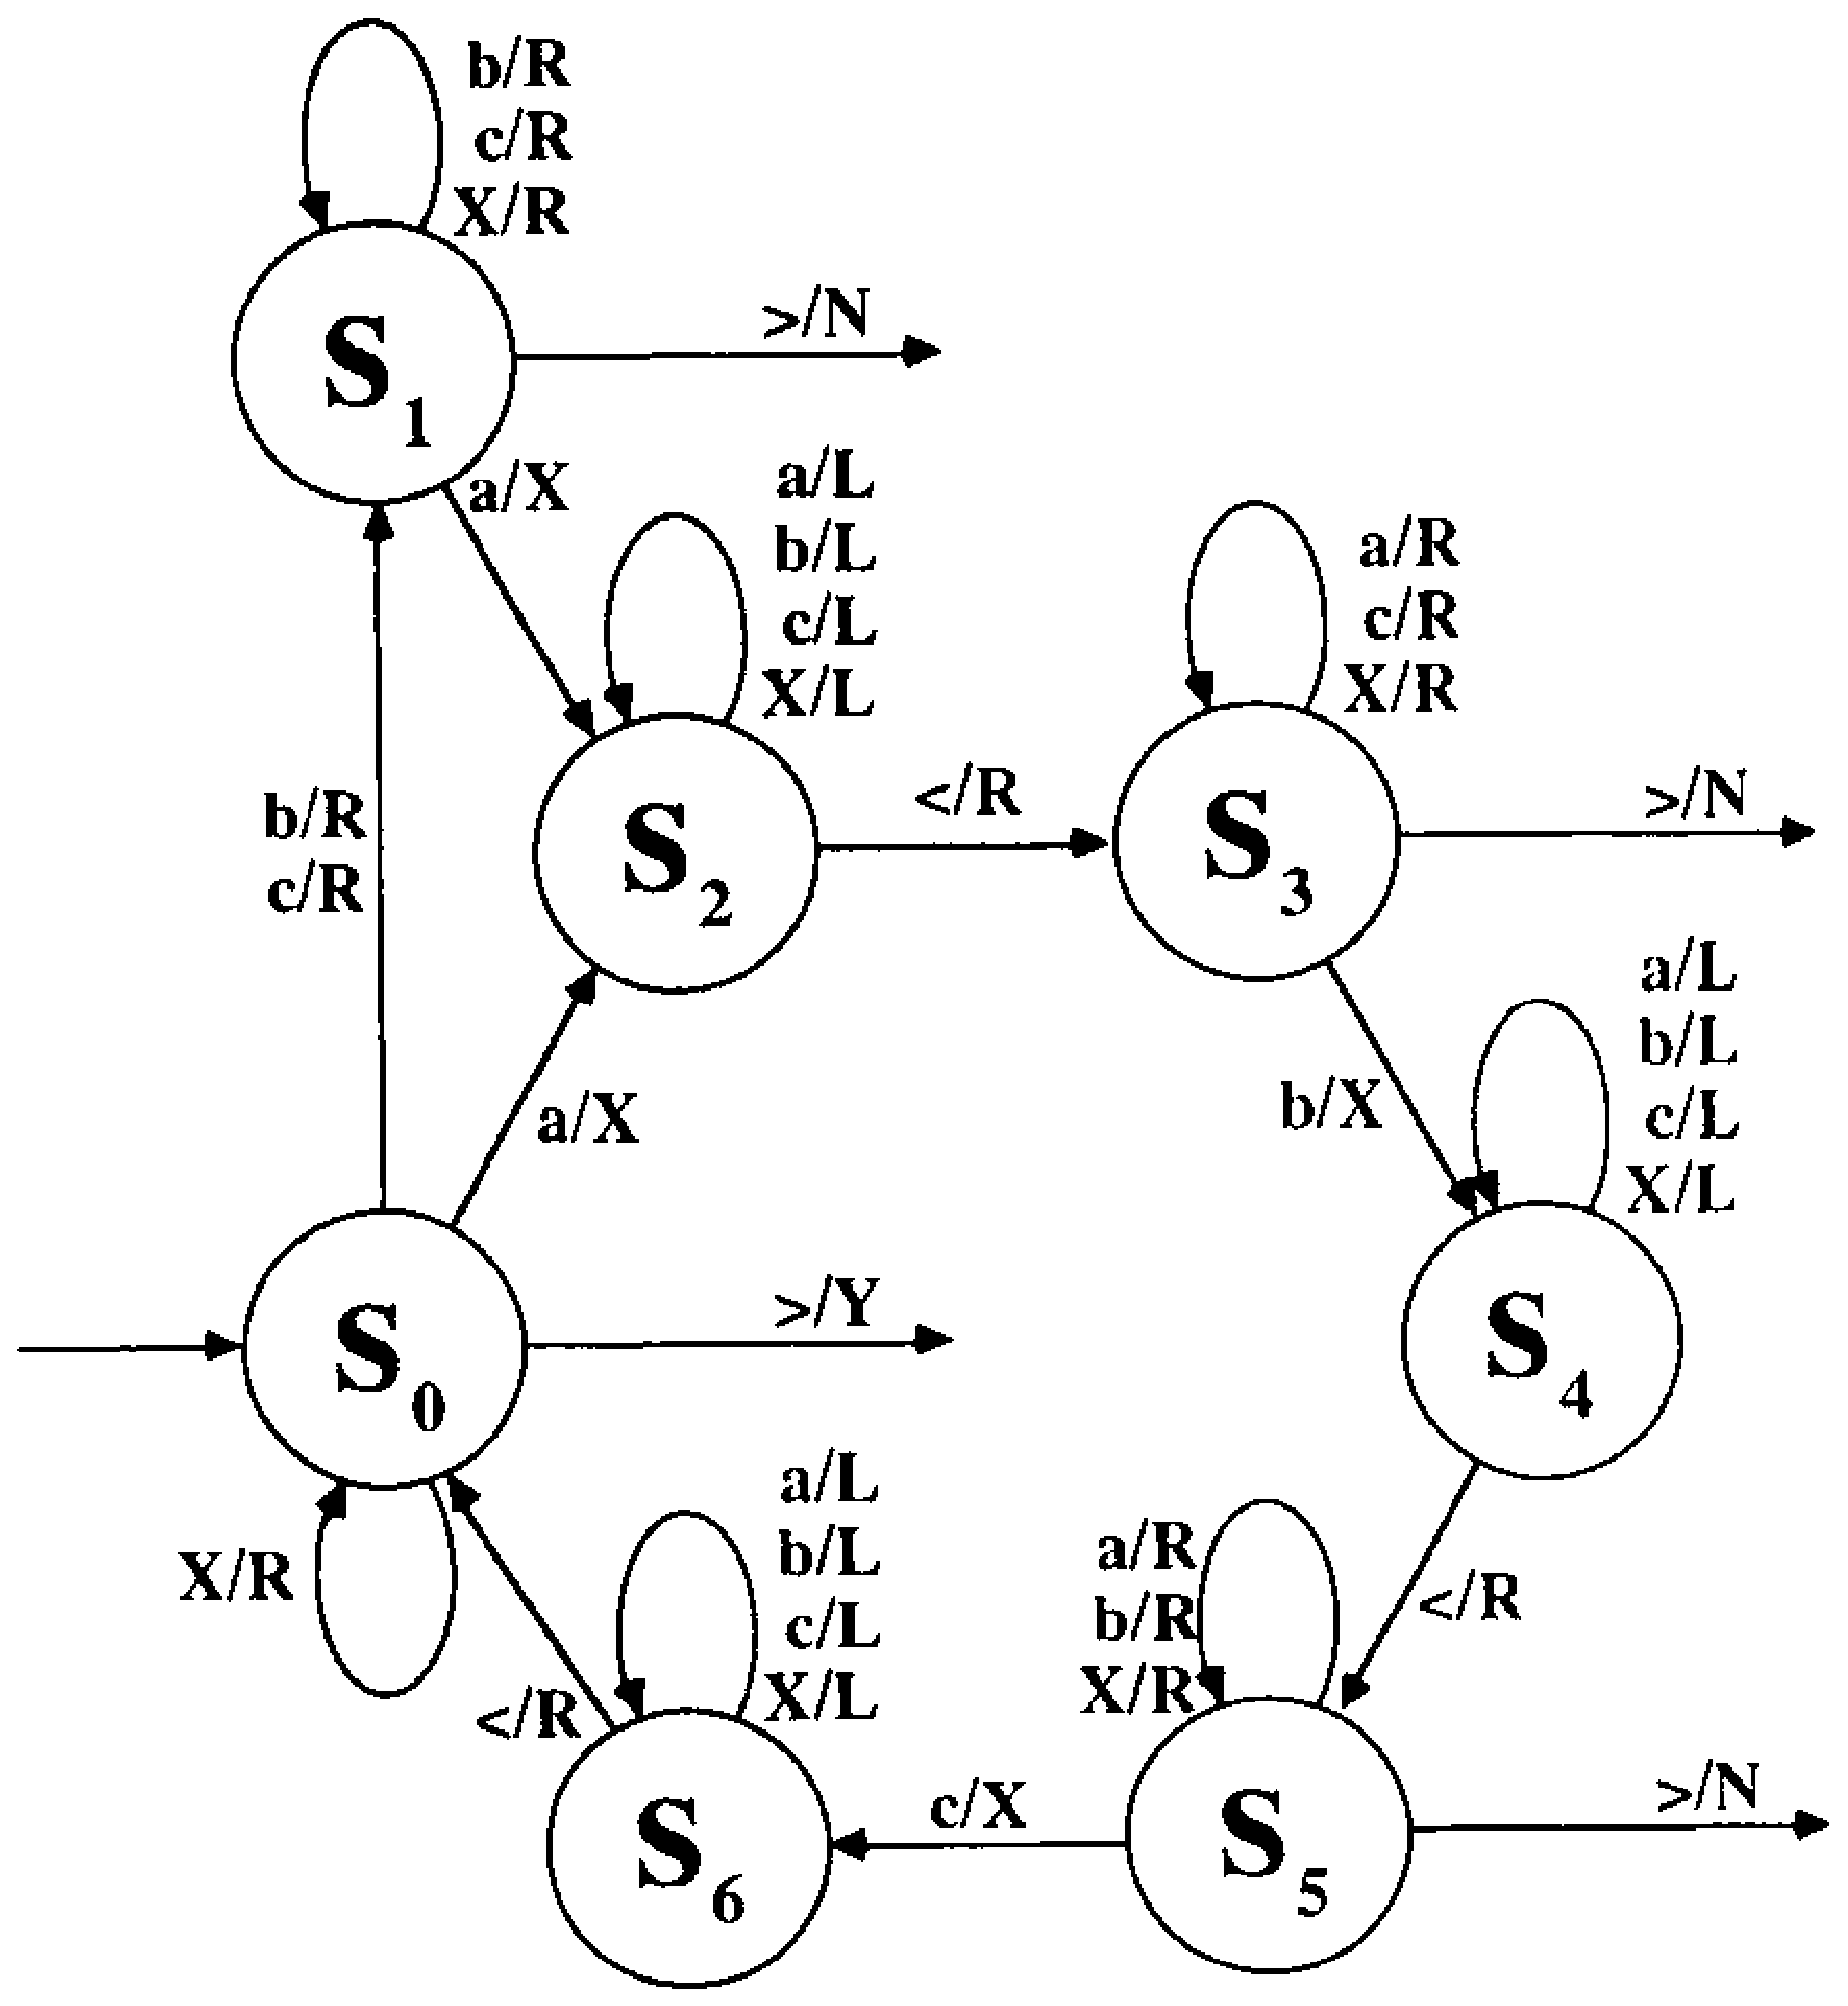
\epsfig{figure=ToFAfigures/fig11-11.eps,width=3.4in}}
\caption{The Turing machine discussed in Example 11.10}\label{fig-11.11}
\end{figure}

% Definition 11.7
\begin{dfn}\label{dfn-11.7}\index{O@\OSIG \ (O-sigma )}\index{L@\LSIG \ (L-sigma )}
For a given alphabet $\Sigma$, let \LSIG\ be the collection of all linear
bounded languages, and let \OSIG\ be the collection of all context-sensitive
(type 1) languages.
\end{dfn}

The proof of Theorem \ref{thm-11.2} can be modified to show that all context-sensitive
languages can be recognized by linear bounded automata. Since context-sensitive
languages do not contain contracting productions, no sentential forms that are
longer than the desired word need be considered. Consequently, the two-tape
Turing machine in Theorem \ref{thm-11.2} can operate as a linear bounded automaton. The
first tape with the input word never changes and thus satisfies the boundary
restriction, while the finite-state control can simply abort any computation on
the second tape that violates the length restriction. Just as Theorem \ref{thm-11.2}
showed that $\ZSIG\subseteq\TSIG$ we now have a relationship between another
pair of cognitive and generative classes.

% Theorem 11.3
\begin{thm}\label{thm-11.3}\index{equivalent!Turing machines}
Let $\Sigma$ be an alphabet. Then $\OSIG\subseteq\LSIG$. That is, every type
1 language is a LBL.

\emph{Proof.} The proof follows from the formalization of the above discussion
(see the exercises).
\end{thm}

We have argued that every type 0 grammar must have an equivalent Turing machine,
and it can conversely be shown that every Turing-acceptable language can be
generated by a type 0 grammar. To do this, it is most convenient to use the very
restrictive criteria for a Turing-acceptable language given in Definition \ref{dfn-11.3},
in which the original input string is not destroyed. For Turing machines which
behave in this fashion, the descriptions of the device configurations bear a
remarkable resemblance to the derivations in a grammar.

\subsection*{Example 11.11}

% Figure 11.12
\begin{figure}
\centerline{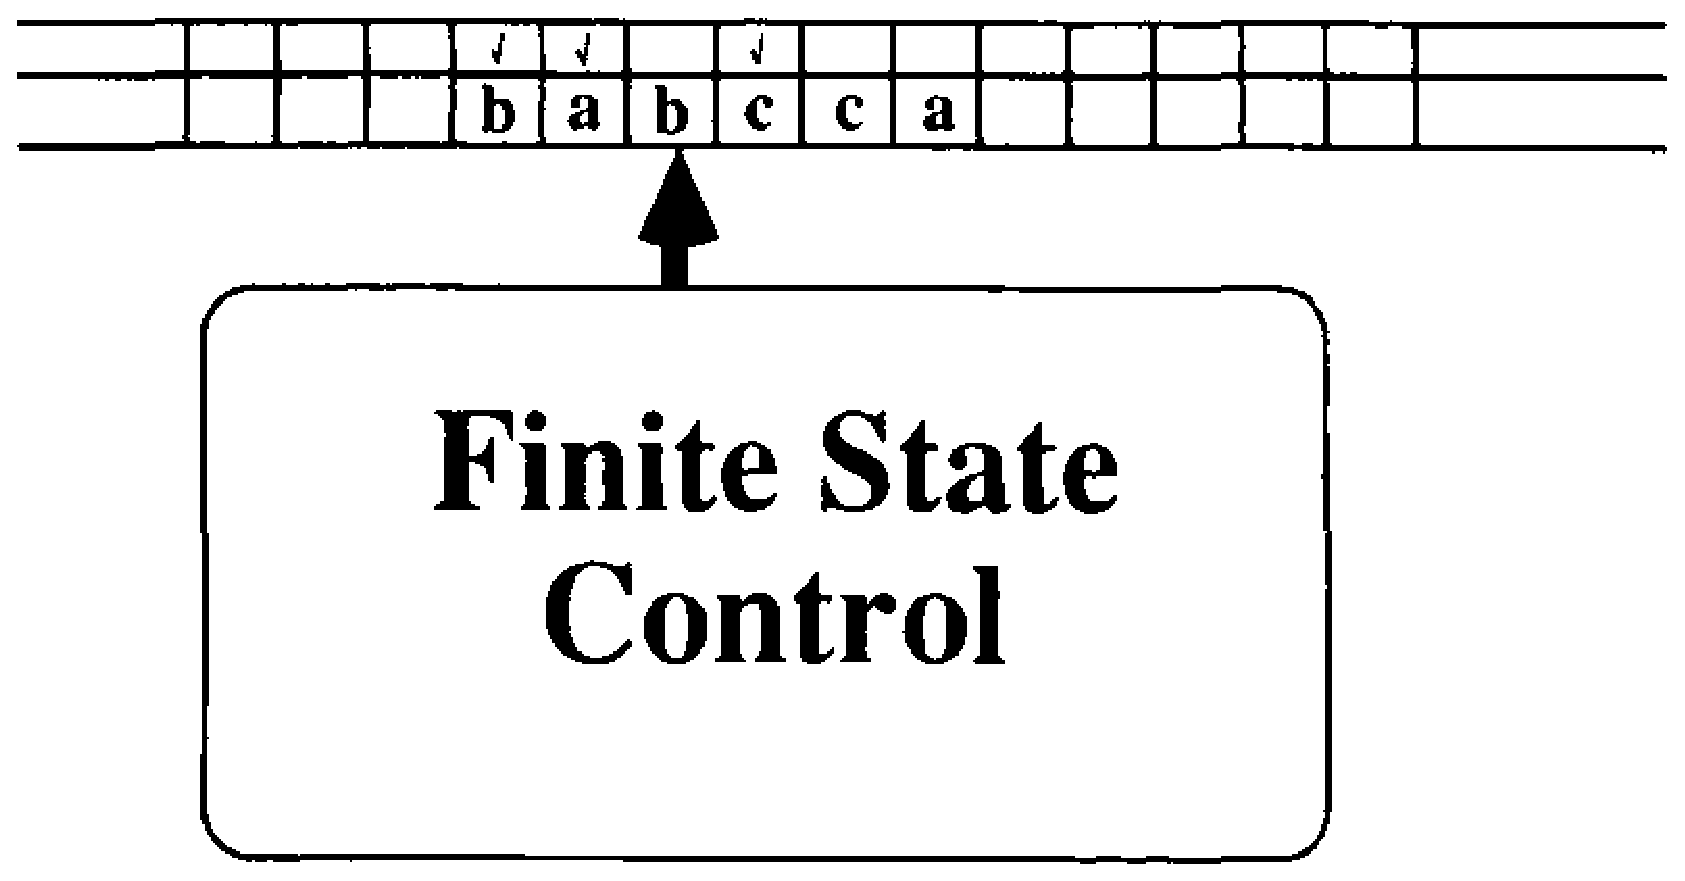
\epsfig{figure=ToFAfigures/fig11-12.eps,width=3.4in}}
\caption{The Turing machine discussed in Example 11.11}\label{fig-11.12}
\end{figure}

Consider again the language $\{x\in\{\pmb{a},\pmb{b},\pmb{c}\}^*|\ \ |x|_{\pmb{a}}
=|x|_{\pmb{b}}=|x|_{\pmb{c}}\}$. As discussed in Example 11.3, the Turing machine
in Figure \ref{fig-11.4} destroys the word originally on the input tape. Figure \ref{fig-11.12}
depicts a slightly more complex Turing machine that restores the original word
just prior to acceptance. It will (fortunately) not generally be necessary for
our purposes to restore rejected words, since there are intricate languages for
which this is not always possible. The modified quintuple is $T=\langle\{\pmb{a},
\pmb{b},\pmb{c}\},\{\pmb{\#},\pmb{A},\pmb{B},\pmb{C},\pmb{Y},\pmb{N}\},\{s_0,s_1,
s_2,s_3,s_4,\\s_5,s_6,s_7,s_8\},s_0,\delta\rangle$, where $\delta$ is as indicated
in the diagram in Figure \ref{fig-11.13}. ``Saving'' the original input string is
accomplished by replacing occurrences of the different letters by distinct
symbols and restoring them later. The implementation reflects one of the first
uses suggested for multiple-track machines: using the second track to check off
input symbols. For legibility, an $\pmb{a}$ with a check mark above it is denoted by
$\pmb{A}$, while an $\pmb{a}$ with no check mark remains an $\pmb{a}$. Similarly,
checked $\pmb{b}$s are represented by $\pmb{B}$ and checked $\pmb{c}$s by
$\pmb{C}$. Thus, if the string $\pmb{BAbCca}$ were on a two-track tape employing
check marks, it would look like
% Get better check symbol than sqrt
\begin{center}\begin{tabular}{ll}
$\!\surd\!\!\surd\ \ \surd$ \\
$\pmb{babcca}$
\end{tabular}\end{center}
The additional states $s_7$ and $s_8$ essentially erase the check marks just
before halting by replacing $\pmb{A}$ with $\pmb{a}$, $\pmb{B}$ with $\pmb{b}$,
and $\pmb{C}$ with $\pmb{c}$.

% Figure 11.13
\begin{figure}
\centerline{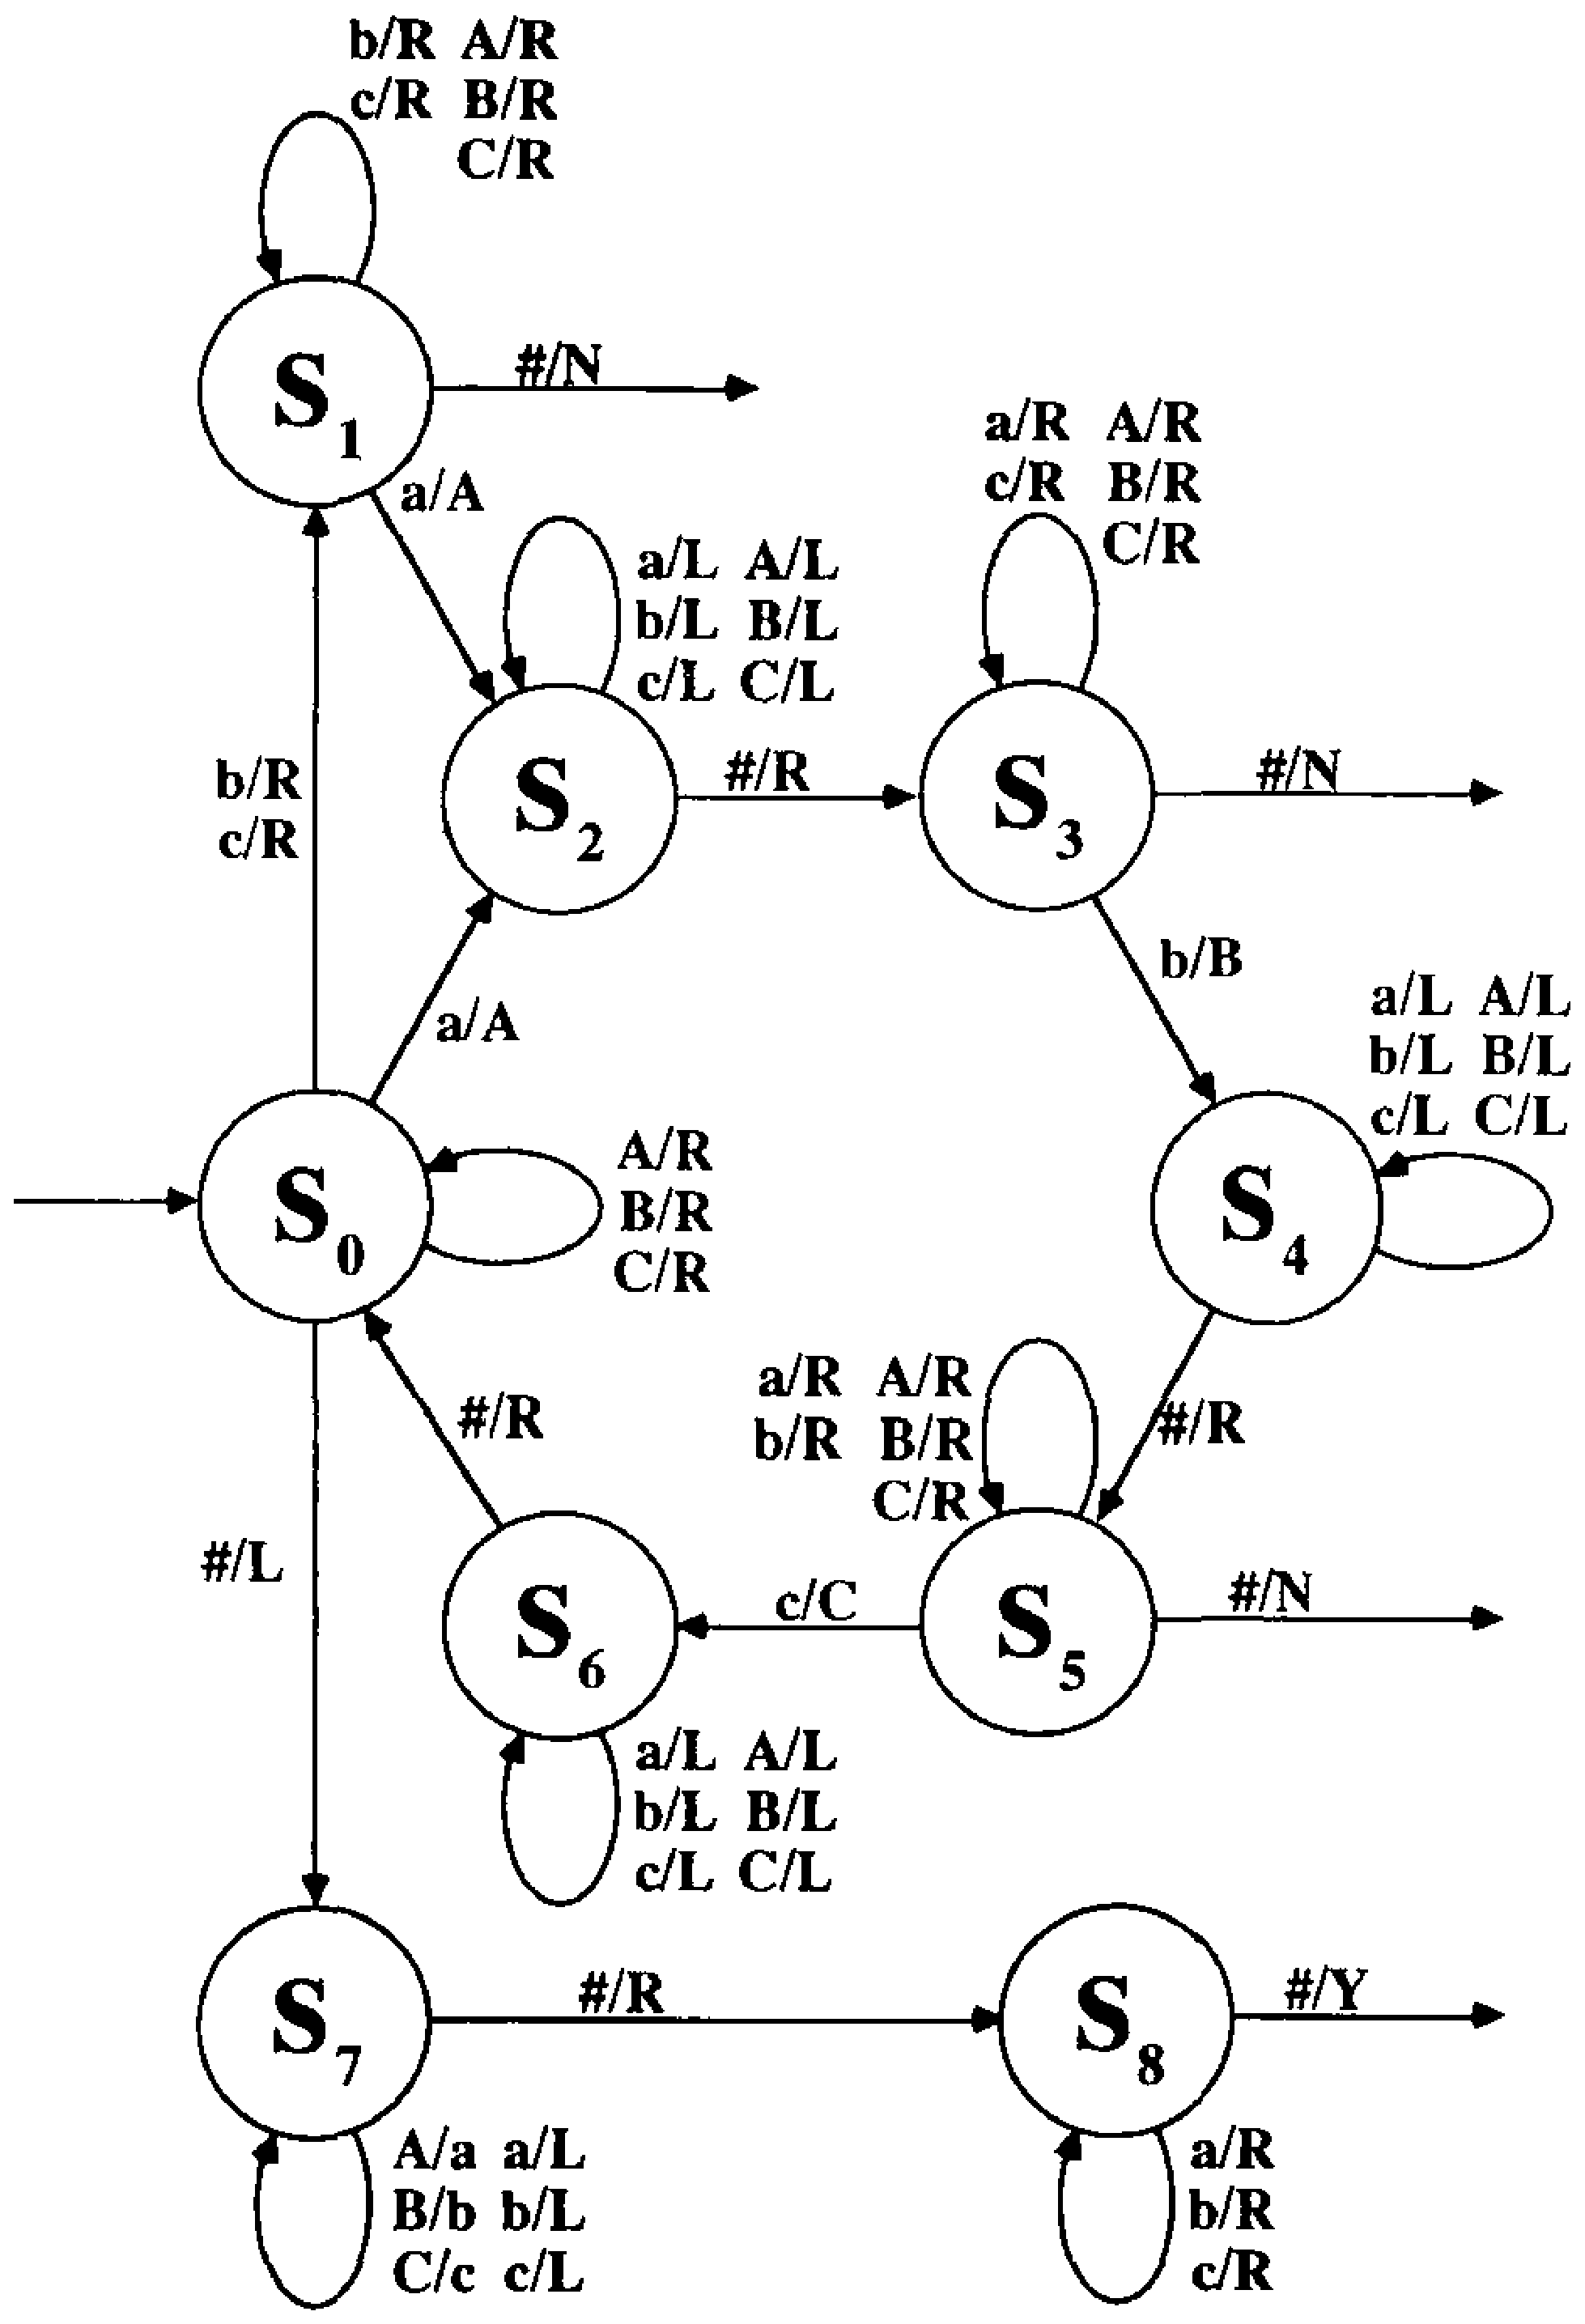
\epsfig{figure=ToFAfigures/fig11-13.eps,height=3.8in}}
\caption{The state transition diagram discussed in Example 11.11}\label{fig-11.13}
\end{figure}

Consider again the input string $\pmb{babcca}$ processed by the Turing machine
in Example 11.3. It is also accepted by this Turing machine because the
following steps show that $s_0\pmb{babcca}\Dvdash\pmb{babccahY}$. Note how
closely the steps correspond with those in Example 11.3. The sequence below also
illustrates how $s_7$ converts the string back to lowercase, after which $s_8$
returns the tape head to the right for acceptance.

\begin{center}\begin{tabular}{r@{ }l@{ }l@{ }l@{ }l@{ }}
$s_0\pmb{babcca}$ & $\vdash\pmb{b}s_1\pmb{abcca}$ & $\vdash\pmb{b}s_2\pmb{Abcca}$
	& $\vdash s_2\pmb{bAbcca}$ & $\vdash$ \\
$s_2\pmb{\#bAbcca}$ & $\vdash s_3\pmb{bAbcca}$ & $\vdash s_4\pmb{BAbcca}$ &
	$\vdash s_4\pmb{\#BAbcca}$ & $\vdash$ \\
$s_5\pmb{BAbcca}$ & $\vdash\pmb{B}s_5\pmb{Abcca}$ & $\vdash\pmb{BA}s_5
	\pmb{bcca}$ & $\vdash\pmb{BAb}s_5\pmb{cca}$ & $\vdash$ \\
$\pmb{BAb}s_6\pmb{Cca}$ & $\vdash\pmb{BA}s_6\pmb{bCca}$ & $\vdash\pmb{B}s_6
	\pmb{AbCca}$ & $\vdash s_6\pmb{BAbCca}$ & $\vdash$ \\
$s_6\pmb{\#BAbCca}$ & $\vdash s_0\pmb{BAbCca}$ &
$\vdash\pmb{B}s_0\pmb{AbCca}$ &
	$\vdash\pmb{BA}s_0\pmb{bCca}$ & $\vdash$ \\
$\pmb{BAb}s_1\pmb{Cca}$ && $\Dvdash s_2\pmb{\#BAbCcA}$ && $\Dvdash$ \\
$\pmb{BA}s_3\pmb{bCca}$ && $\Dvdash s_4\pmb{\#BABCcA}$ && $\Dvdash$ \\
$\pmb{BABC}s_5\pmb{cA}$ && $\Dvdash s_6\pmb{\#BABCCA}$ && $\Dvdash$ \\
$\pmb{BABCCA}s_0$ & $\vdash\pmb{BABCC}s_7\pmb{A}$ & $\vdash\pmb{BABCC}s_7
	\pmb{a}$ & $\vdash\pmb{BABC}s_7\pmb{Ca}$ & $\vdash$ \\
$\pmb{BABC}s_7\pmb{ca}$ && $\Dvdash s_7\pmb{babcca}$ & $\vdash
s_7\pmb{\#babcca}$
	& $\vdash$ \\
$s_8\pmb{babcca}$ & $\vdash\pmb{b}s_8\pmb{abcca}$ & $\Dvdash\pmb{babcca}s_8$
&&
	$\vdash$ \\
$\pmb{babccahY}$
\end{tabular}\end{center}

If occurrences of the machine transition symbol $\vdash$ are replaced by the
derivation symbol $\Rightarrow$, the above sequence would look remarkably like a
derivation in a type 0 grammar. Indeed, we would like to construct a grammar in
which sentential forms like $\pmb{b}s_1\pmb{abcca}$ could be derived from
$s_0\pmb{babcca}$ in one step. Since the machine changed configurations because
of the transition rule $\delta(s_0,\pmb{b})=\langle s_1,\pmb{R}\rangle$, this
transition should have a corresponding production of the form $s_0\pmb{b}
\rightarrow\pmb{b}s_1$. Each transition in the Turing machine will be
responsible for similar productions.

Unfortunately, the correspondence between transition rules and productions is
complicated by the fact that the tape head may occasionally scan blank cells,
which must then be added to the sentential form. The special characters `$[$' and
`$]$' will bracket the sentential form throughout this stage of the derivation and
will indicate the current left and right limits of the tape head travel,
respectively. Attempting to move left past the conceptual position of `$[$' (or
right past the position of `$]$'\,) will result in the addition of a blank symbol to
the sentential form.

To generate the words accepted by a Turing machine, our grammar will randomly
generate a word over $\Sigma$, delimit it by brackets, and insert the symbol for
the start state at the left edge. The rules derived from the transitions should
then be able to transform a string such as $[s_0\pmb{babcca\#}]$ into
$[\pmb{\#babccahY\#}]$. Since only the letters in $\Sigma$ will be considered
terminal symbols, the symbols $[$, $]$, $\pmb{\#}$, and $\pmb{Y}$ are
nonterminals, and the derivation will not yet be complete. To derive terminal
strings for just the accepted words, the presence of $\pmb{Y}$ will allow
further productions to delete those remaining nonterminals.

% Definition 11.8
\begin{dfn}\label{dfn-11.8}\index{Turing machine!corresponding grammar}
Given a Turing machine $M=\langle\Sigma,\Gamma,S,s_0,\delta\rangle$, the grammar
corresponding to $M$, $G_M$, is given by $G_M=\langle\Sigma,\Gamma\cup S\cup\{Z,
W,U,V,[,]\},Z,P_M\rangle$, where $P_M$ contains the following classes of
productions:
\begin{enumerate}
\item $Z\rightarrow[W\pmb{\#}]\in P_M$ \\
$(\forall \pmb{a}\in\Sigma)([W\rightarrow[W\pmb{a}\in P_M)$ \\
$W\rightarrow s_0\in P_M$

\item Each printing transition gives rise to a production rule as follows
\[ (\forall s\in S)(\forall t\in S\cup\{h\})(\forall\pmb{a},\pmb{b}\in\Sigma\cup
	\Gamma)(\text{if }\delta(s,\pmb{a})=\langle t,\pmb{b}\rangle,
	\text{ then }s\pmb{a}\rightarrow t\pmb{b}\in P_M) \]
Each move right gives rise to a production rule as follows
\[ (\forall s,t\in S)(\forall\pmb{a}\in\Sigma\cup\Gamma)(\text{if }\delta(s,
	\pmb{a})=\langle t,\pmb{R}\rangle,\text{ then }s\pmb{a}\rightarrow
	\pmb{a}t\in P_M) \]
If $\pmb{a}=\pmb{\#}$, an additional production is needed:
\[ (\forall s,t\in S)(\text{if }\delta(s,\pmb{\#})=\langle t,\pmb{R}\rangle,
	\text{ then }s]\rightarrow\pmb{\#}t]\in P_M) \]
Each move left gives rise to a production rule as follows
\begin{center}\begin{tabular}{l}
$(\forall s,t\in S)(\forall\pmb{a}\in\Sigma\cup\Gamma)$ \\
$(\text{if }\delta(s,\pmb{a})=\langle t,\pmb{L}\rangle,\text{ then }[s\pmb{a}
	\rightarrow [t\pmb{\#a}\in P_M\wedge (\forall\pmb{d}\in\Sigma\cup\Gamma)
	(\pmb{d}s\pmb{a}\rightarrow t\pmb{da}\in P_M))$
\end{tabular}\end{center}

\item $h\pmb{Y}\rightarrow U\in P_M$ \\
$U\pmb{\#}\rightarrow U\in P_M$ \\
$U]\rightarrow V\in P_M$ \\
$(\forall\pmb{a}\in\Sigma)(\pmb{a}V\rightarrow V\pmb{a}\in P_M)$ \\
$\pmb{\#}V\rightarrow V\in P_M$ \\
$[V\rightarrow \lambda\in P_M$
\end{enumerate}
\end{dfn}

The rules in class 1 are intended to generate all words of the form $[s_0x
\pmb{\#}]$, where $x$ is an arbitrary member of $\Sigma^*$. The remaining rules
are defined in such a way that only those strings $x$ that are recognized by $M$
can successfully produce a terminal string. Note that once $W$ is replaced by
$s_0$, neither $Z$ nor $W$ can appear in a later sentential form. After $s_0$ is
generated, the rules in class 2 may apply. It can be inductively argued that the
derivations arising from the application of these rules directly reflect the
changes in the configuration of the Turing machine (see Theorem \ref{thm-11.4}).

None of the class 3 productions can be used until the point at which the halt
state would be reached in the corresponding computation. Since $h\notin S$, none
of the class 2 productions can then be used. Only if $\pmb{Y}$ was written to tape as
the Turing machine halted will the production $h\pmb{Y}\rightarrow U$ be
applicable. $U$ will then delete the trailing blanks and $]$ from the sentential
form, and then $V$ will percolate to the left, removing the leading blanks and
the final nonterminal $[$, leaving only the terminal string $x$ in the
(completed) sentential form. The following example illustrates a derivation
stemming from a typical Turing machine.

\subsection*{Example 11.12}

Consider the Turing machine $T$ in Figure \ref{fig-11.13} and the corresponding grammar
$G_T$. Among the many possible derivations involving the class 1 productions is
\begin{center}\begin{tabular}{r@{ $\Rightarrow$ }l}
$Z$ & $[W\pmb{\#}]\Rightarrow[W\pmb{a\#}]\Rightarrow[W\pmb{ca\#}]\Rightarrow
	[W\pmb{cca\#}]\Rightarrow[W\pmb{bcca\#}]\Rightarrow[W\pmb{abcca\#}]$ \\
& $[W\pmb{babcca\#}]\Rightarrow[s_0\pmb{babcca\#}]$
\end{tabular}\end{center}
Only class 2 productions apply at this point, and there is exactly one
derivation applicable at each step in the following sequence.
\begin{center}\begin{tabular}{r@{ }l@{ }l@{ }l@{ }l}
$[s_0\pmb{babcca\#}]$ & $\Rightarrow[\pmb{b}s_1\pmb{abcca\#}]$ & $\Rightarrow
	[\pmb{b}s_2\pmb{Abcca\#}]$ & $\Rightarrow[s_2\pmb{bAbcca\#}]$ &
	$\Rightarrow$ \\
$[s_2\pmb{\#bAbcca\#}]$ & $\Rightarrow[\pmb{\#}s_3\pmb{bAbcca\#}]$ &
	$\Rightarrow[\pmb{\#}s_4\pmb{BAbcca\#}]$ & $\Rightarrow[s_4\pmb{\#BAbcca
	\#}]$ & $\Rightarrow$ \\
$[\pmb{\#}s_5\pmb{BAbcca\#}]$ & $\Rightarrow[\pmb{\#B}s_5\pmb{Abcca\#}]$ &
	$\Rightarrow[\pmb{\#BA}s_5\pmb{bcca\#}]$ & $\Rightarrow[\pmb{\#BAb}s_5
	\pmb{cca\#}]$ & $\Rightarrow$ \\
$[\pmb{\#BAb}s_6\pmb{Cca\#}]$ & $\Rightarrow[\pmb{\#BA}s_6\pmb{bCca\#}]$ & 
	$\Rightarrow[\pmb{\#B}s_6\pmb{AbCca\#}]$ & $\Rightarrow[\pmb{\#}s_6
	\pmb{BAbCca\#}]$ & $\Rightarrow$ \\
$[s_6\pmb{\#BAbCca\#}]$ & $\Rightarrow[\pmb{\#}s_0\pmb{BAbCca\#}]$ &
	$\Rightarrow[\pmb{\#B}s_0\pmb{AbCca\#}]$ & $\Rightarrow[\pmb{\#BA}s_0
	\pmb{bCca\#}]$ & $\Rightarrow$ \\
$[\pmb{\#BAb}s_1\pmb{Cca\#}]$ && $\DRightarrow[s_2\pmb{\#BAbCcA\#}]$ &&
	$\DRightarrow$ \\
$[\pmb{\#BA}s_3\pmb{bCcA\#}]$ && $\DRightarrow[s_4\pmb{\#BABCcA\#}]$ &&
	$\DRightarrow$ \\
$[\pmb{\#BABC}s_5\pmb{cA\#}]$ && $\DRightarrow[s_6\pmb{\#BABCCA\#}]$ &&
	$\DRightarrow$ \\
$[\pmb{\#BABCCA}s_0\pmb{\#}]$ & $\Rightarrow[\pmb{\#BABCC}s_7\pmb{A\#}]$ &
	$\Rightarrow[\pmb{\#BABCC}s_7\pmb{a\#}]$ & $\Rightarrow[\pmb{\#BABC}s_7
	\pmb{Ca\#}]$ & $\Rightarrow$ \\
$[\pmb{\#BABC}s_7\pmb{ca\#}]$ && $\DRightarrow[\pmb{\#}s_7\pmb{babcca\#}]$ &
	$\Rightarrow[s_7\pmb{\#babcca\#}]$ & $\Rightarrow$ \\
$[\pmb{\#}s_8\pmb{babcca\#}]$ & $\Rightarrow[\pmb{\#b}s_8\pmb{abcca\#}]$ & 
	$\DRightarrow[\pmb{\#babcca}s_8\pmb{\#}]$ && $\Rightarrow$ \\
$[\pmb{\#babcca}h\pmb{Y}]$
\end{tabular}\end{center}
In Turing machines where the tape head travels further afield, there may be
many more blanks enclosed within the brackets. At this point, the class 3
productions take over to tidy up the string:
\begin{center}\begin{tabular}{l}
$[\pmb{\#babcca}h\pmb{Y}]\Rightarrow[\pmb{\#babcca}U]\Rightarrow[\pmb{\#babcca}V
	\Rightarrow[\pmb{\#babcc}V\pmb{a}$ \\
$\Rightarrow[\pmb{\#babc}V\pmb{ca}\Rightarrow[\pmb{\#bab}V\pmb{cca}\Rightarrow
	[\pmb{\#ba}V\pmb{bcca}\Rightarrow[\pmb{\#b}V\pmb{abcca}$ \\
$\Rightarrow[\pmb{\#}V\pmb{babcca}\Rightarrow[V\pmb{babcca}\Rightarrow
	\pmb{babcca}$
\end{tabular}\end{center}
As expected, $\pmb{babcca}\in L(G_T)$.

It is interesting to observe that the only stage in which a choice of productions
is available is during the replacement of the nonterminal $W$. Once a candidate
string is so chosen, the determinism of the Turing machine forces the remainder
of the derivation to be unique. This is true even for strings that were not
accepted by the Turing machine: if class 2 productions are applied to $[s_0\pmb{
baa\#}]$, there is exactly one derivation sequence for this sequential form, and
it leads to $[\pmb{BAa}s_5\pmb{\#}]$ and then $[\pmb{BAa}h\pmb{N}]$. No productions
apply to this sentential form, and thus no terminal string will be generated.
The relationship between strings accepted by the Turing machine and the strings
generated by the corresponding grammar is at the heart of the following theorem.

% Theorem 11.4
\begin{thm}\label{thm-11.4}
Let $\Sigma$ be an alphabet. Then $\TSIG\subseteq\ZSIG$. That is, every
Turing-acceptable language can be generated by a type 0 grammar.

\emph{Proof.} Let $M$ be a Turing machine $M=\langle\Sigma,\Gamma,S,s_0,\delta
\rangle$, and let
\[ L(M) = \{x\in\Sigma^*|\ s_0x\Dvdash xh\pmb{Y}\}, \]
as specified in the most restrictive sense of a Turing-acceptable language
(Definition \ref{dfn-11.3}). Consider the grammar $G_M$ corresponding to $M$, as given in
Definition \ref{dfn-11.8}. The previous discussion of $G_M$ provided a general sense of the
way in which the productions could be used and justified that they could not be
combined in unexpected ways. A rigorous proof requires an explicit formal
statement of the general properties that have been discussed. A trivial
induction on the length of $x$ shows that by using just the productions in
class 1
	\[ (\forall x\in\Sigma^*)(Z\ \DRightarrow[s_0x\pmb{\#}]) \]

Another induction argument establishes the correspondence between sequences of
applications of the class 2 productions and sequences of moves in the Turing
machine. Specifically, by inducting on the number of transitions, it can be
shown that
\begin{center}\begin{tabular}{l}
$(\forall s,t\in S\cup\{h\})(\forall\alpha,\beta,\gamma,\omega\in(\Sigma\cup
	\Gamma)^*)$ \\
$(\alpha s\beta\Dvdash\gamma t\omega$ iff $(\exists i,j,m,n\in\NN)([\pmb{\#}^i
	\alpha s\beta\pmb{\#}^j]\ \DRightarrow[\pmb{\#}^m\gamma t\omega\pmb{\#}
	^n]))$
\end{tabular}\end{center}
The actual number of padded blanks is related to the extent of the tape head
movement, but this is not important for our purposes. The essential observation
is that a move sequence in $M$ is related to a derivation sequence in $G_M$,
with perhaps some change in the number of blanks at either end. The above
statement was stated in full generality to facilitate the induction proof (see
the exercises). We need apply it in a very limited sense, as stated below.
\[ (\forall\alpha,\beta,\gamma,\omega\in(\Sigma\cup\Gamma)^*)(s_0x\Dvdash x
	h\pmb{Y}\text{ iff }(\exists m,n\in\NN)([s_0x\pmb{\#}]\ \DRightarrow
	[\pmb{\#}^mxh\pmb{Y\#}^n])) \]
Observe that the productions in class 3 cannot be used unless $h\pmb{Y}$ appears
on the tape after a finite number of steps. As discussed earlier, the presence
of $h\pmb{Y}$ triggers the class 3 productions, which remove all the remaining
nonterminals. Thus,
\[ (\forall x\in\Sigma^*)(s_0x\Dvdash xh\pmb{Y}\text{ iff }Z\ \DRightarrow[s_0x
	\pmb{\#}]\ \DRightarrow[\pmb{\#}^mxh\pmb{Y\#}^n]\ \DRightarrow x) \]
which implies that $L(M)=L(G_M)$.
\end{thm}

Since every Turing machine has an equivalent type 0 grammar and every type 0
grammar generates a Turing-acceptable language, we have two ways of representing
the same class of languages.

% Corollary 11.1
\begin{cor}\label{cor-11.1}
The class of languages generated by type 0 grammars is exactly the
Turing-acceptable languages. That is, $\ZSIG=\TSIG$.

\emph{Proof.} The proof follows immediately from Theorems \ref{thm-11.2} and \ref{thm-11.4}.
\end{cor}

As will be seen in Chapter \ref{ch-12}, the linear bounded languages are a distinctly
smaller class than the Turing-acceptable languages. Theorem \ref{thm-11.3} showed that
$\OSIG\subseteq\LSIG$, and a technique similar to that used in Theorem \ref{thm-11.4} will
show that $\LSIG\subseteq\OSIG$. That is, we can show that every linear bounded
automaton has an equivalent context-sensitive grammar. Note that the class 1 and
2 productions in Definition \ref{dfn-11.8} contained no contracting productions; it was
only when the class 3 productions were applied that the sentential form might
shrink. When dealing with linear bounded automata, the tape head is restricted
to the portion of the tape containing the input string, so there will be no
extraneous blanks to delete. The input word on the tape of a linear bounded
automaton is bracketed by distinct symbols \< and \>, which might be used in the
corresponding grammar in a fashion similar to $[$ and $]$. These would be
\emph{immovable} in the sense that no new blanks would be inserted between them
and the rest of the bracketed word. Unfortunately, in Definition \ref{dfn-11.8} the
delimiters $[$ and $]$ must eventually disappear, shortening the sentential
form. No such shrinking can occur if we hope to produce a context-sensitive
grammar.

To overcome this difficulty, it is useful to imagine a three-track tape with
the input word on the middle track and the delimiter - on the upper track of the
tape above the first symbol of the word. Another - will occur on the lower track
below the last character of the input string. These markers will serve as guides
to prevent the tape head from moving past the limits of the input word. For
example, if the linear bounded automaton contained the word $\<\pmb{babcca}\>$
on its input tape, the tape for the corresponding three-track automaton would be
as pictured in Figure \ref{fig-11.14a}. If the word were accepted, the tape would
eventually reach the configuration shown in Figure \ref{fig-11.14b} as it halted, printing
$\pmb{Y}$ on the lower track. It is a relatively simple task to convert a linear
bounded automaton into a three-track automaton, where the tape head never moves
left of the tape cell with the - in the upper track, and never moves right of
the cell with the - in the lower track (see the exercises). We will refer to
such an automaton as a \emph{strict linear bounded automaton}. The definitions
used will depend on the upper and lower track markers occurring in different
cells, which makes the representation of words of length less than two awkward.
Since this construct is motivated by a need to find a context-sensitive grammar,
we will simply modify the resulting grammar to explicitly generate any such
short words and not rely on the above formalism.


\setcounter{figure}{0}
\renewcommand{\thefigure}{\arabic{chapter}.14\alph{figure}}
% Figure 11.14a
\begin{figure}
\centerline{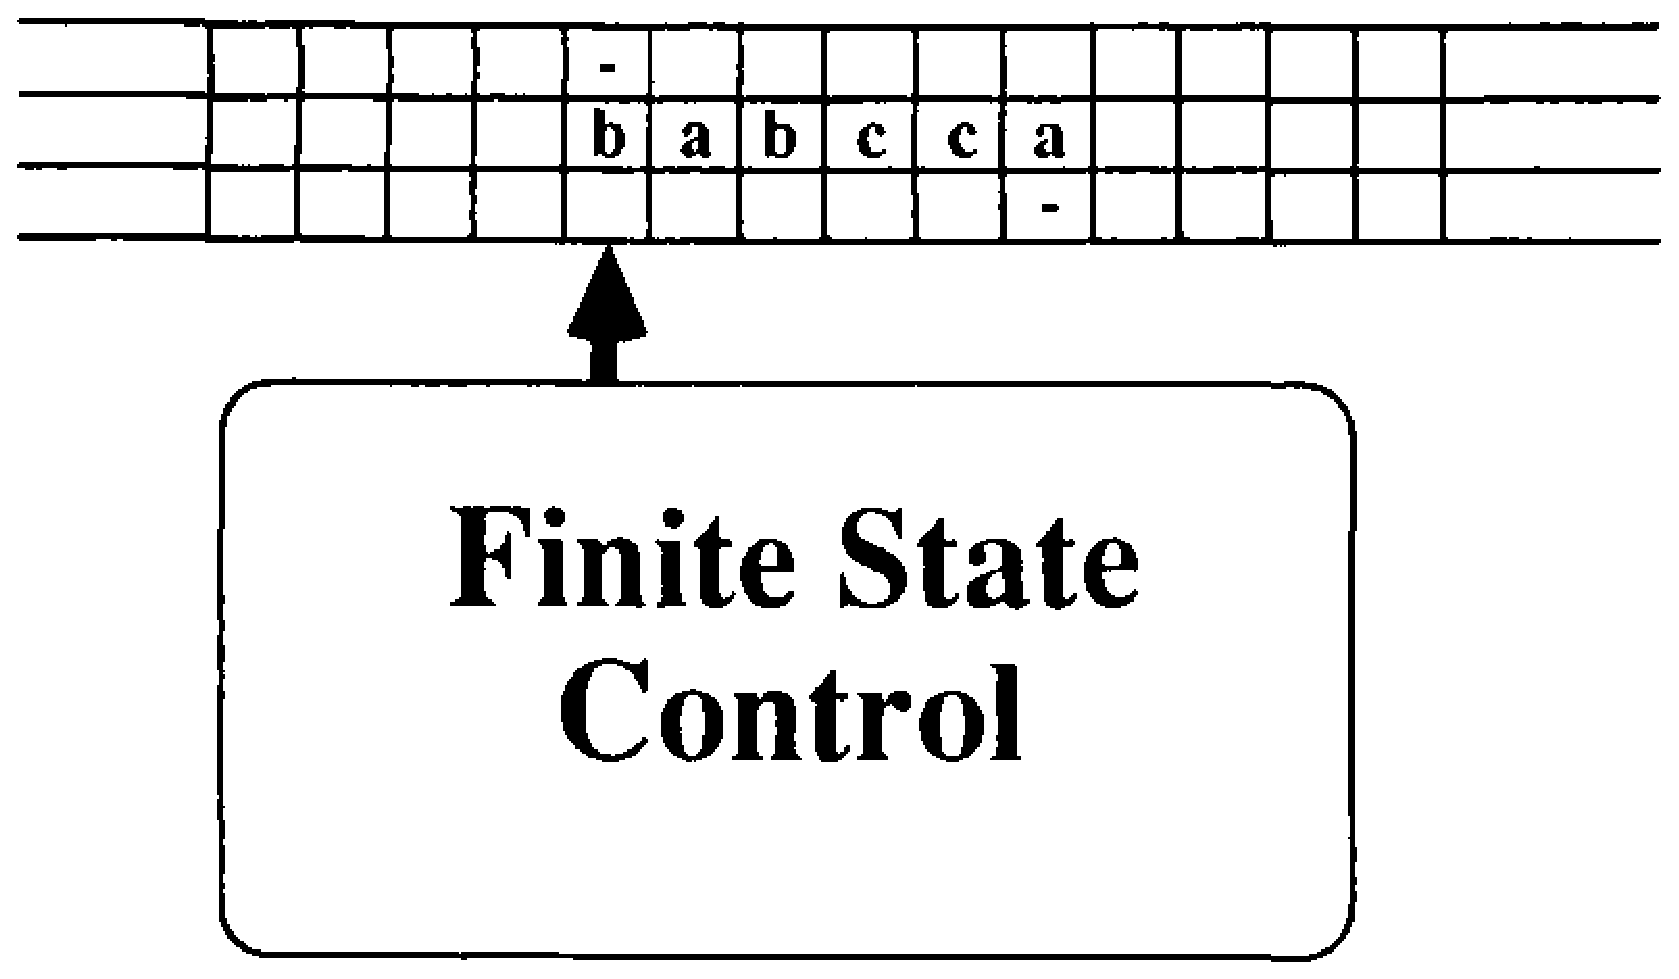
\epsfig{figure=ToFAfigures/fig11-14a.eps,width=3.4in}}
\caption{A three-track Turing machine employing delimiters}\label{fig-11.14a}
\end{figure}

% Figure 11.14b
\begin{figure}
\centerline{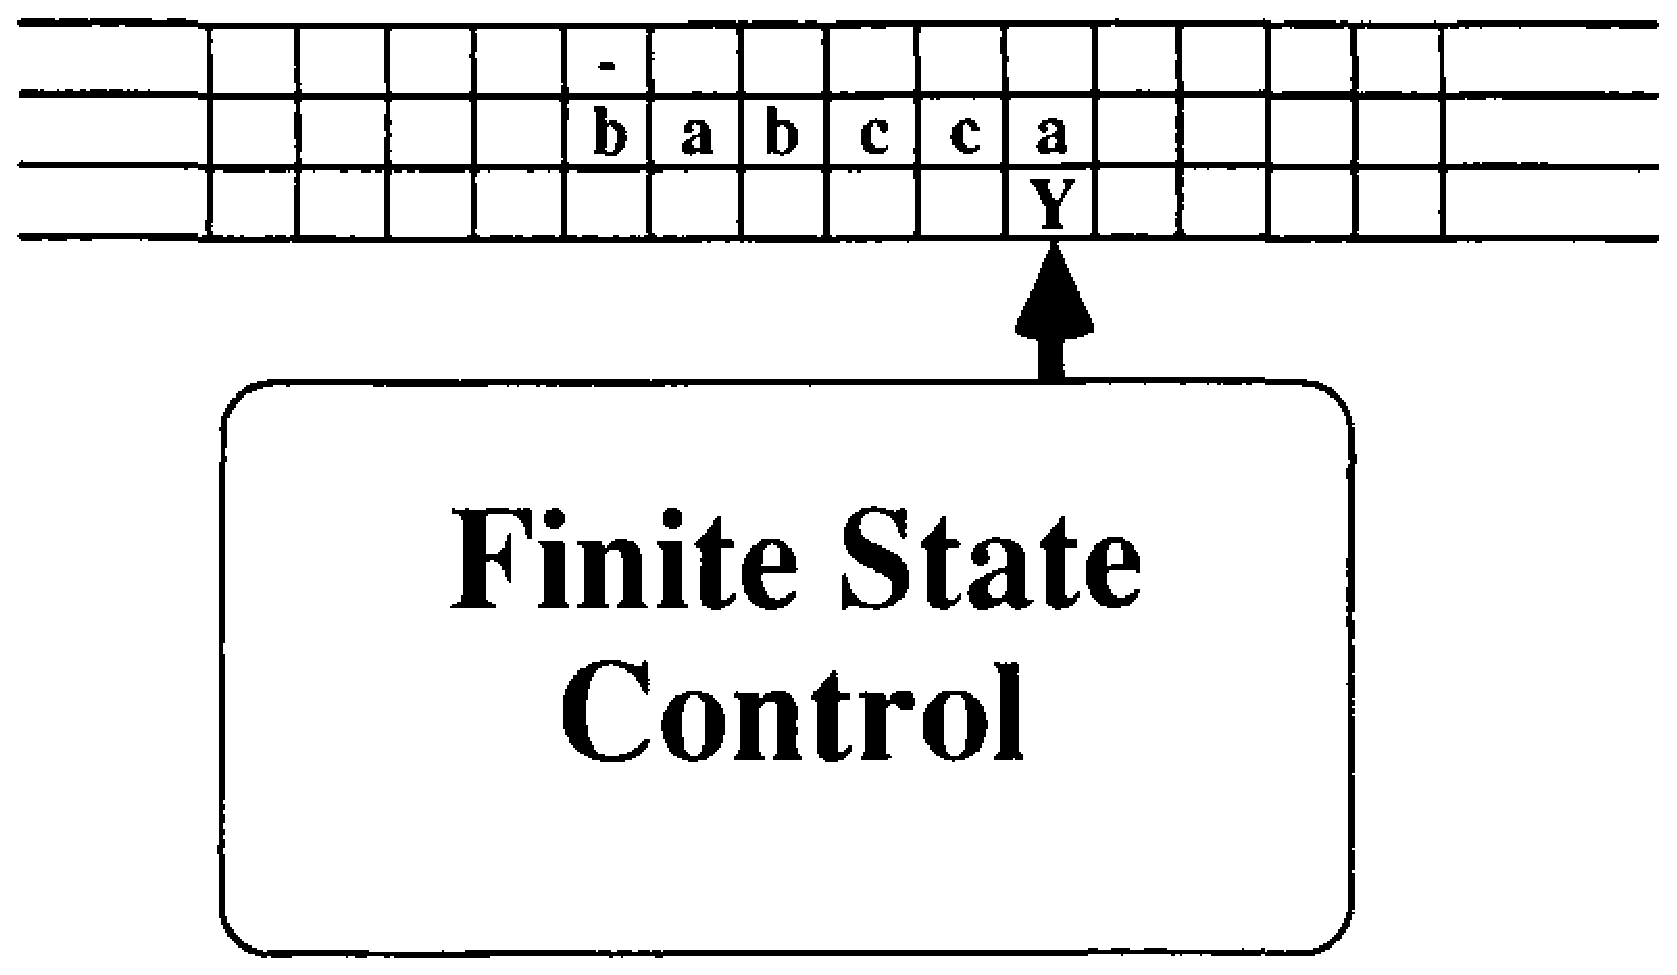
\epsfig{figure=ToFAfigures/fig11-14b.eps,width=3.4in}}
\caption{An accepting configuration}\label{fig-11.14b}
\end{figure}
\setcounter{figure}{14}                       %nasty kluge
\renewcommand{\thefigure}{\arabic{chapter}.\arabic{figure}}

\subsection*{Example 11.13}

Consider the linear-bounded automaton discussed in Example 11.10, which
accepted $\{x\in\{\pmb{a},\pmb{b},\pmb{c}\}^*|\ \ |x|_{\pmb{a}}=|x|_{\pmb{b}} =
|x|_{\pmb{c}}\}$. As suggested by the exercises, this can be modified to form
the three-track strict linear bounded automaton shown in Figure \ref{fig-11.15}, which
accepts $\{x\in\{\pmb{a},\pmb{b},\pmb{c}\}^*|\ \ |x|\geq 2\wedge |x|_{\pmb{a}} =
|x|_{\pmb{b}} = |x|_{\pmb{c}}\}$. To avoid explicitly mentioning the three
tracks, a cell containing $\pmb{b}$ on the middle track and $-$ on the upper
track is denoted by the single symbol \pmb{$\overline{b}$}, a cell containing $\pmb{A}$ on
the middle track and $-$ on the lower track is shown as \pmb{$\underline{A}$}, and so on.
Thus, the six original symbols in $\{\pmb{a},\pmb{b},\pmb{c},\pmb{A},\pmb{B},
\pmb{C}\}$ give rise to six other symbols employing the overbar $^-$, six
more using the underscore $\underline{\ \ }$, and some symbols indicating
acceptance (or possibly rejection), such as $\pmb{a}_{\pmb{Y}}$ (or $\pmb{C}_{
\pmb{N}}$). For clarity, only those combinations that can actually occur in a
transition sequence are shown in Figure \ref{fig-11.15}. The sequence of moves that would
transform the tape from the configuration shown in Figure \ref{fig-11.14a} to that of
Figure \ref{fig-11.14b} is shown below.

\begin{center}\begin{tabular}{r@{ }l@{ }l@{ }l@{ }l}
$s_0\overline{\pmb{b}}\pmb{abcc}\underline{\pmb{a}}$ & $\vdash\overline{\pmb{b}}s_1\pmb{abcc}
	\underline{\pmb{a}}$ & $\vdash\overline{\pmb{b}}s_2\pmb{Abcc}\underline{
	\pmb{a}}$ & $\vdash s_2\overline{\pmb{b}}\pmb{Abcc}\underline{\pmb{a}}$ & $\vdash$ \\
& $\ \ \ s_3\overline{\pmb{b}}\pmb{Abcc}\underline{\pmb{a}}$ & $\vdash s_4\overline{\pmb{B}}\pmb{Abcc}\underline{\pmb{a}}$ &
	$\vdash$ \\
$s_5\overline{\pmb{B}}\pmb{Abcc}\underline{\pmb{a}}$ & $\vdash\overline{\pmb{B}}s_5\pmb{Abcc}
	\underline{\pmb{a}}$ & $\vdash\overline{\pmb{B}}\pmb{A}s_5\pmb{bcc}\underline{\pmb{a}}$ &
	$\vdash\overline{\pmb{B}}\pmb{Ab}s_5\pmb{cc}\underline{\pmb{a}}$ & $\vdash$ \\
$\overline{\pmb{B}}\pmb{Ab}s_6\pmb{Cc}\underline{\pmb{a}}$ & $\vdash\overline{\pmb{B}}\pmb{A}s_6\pmb{bCc}
	\underline{\pmb{a}}$ & $\vdash\overline{\pmb{B}}s_6\pmb{AbCc}\underline{\pmb{a}}$ &
	$\vdash s_6\overline{\pmb{B}}\pmb{AbCc}\underline{\pmb{a}}$ & $\vdash$ \\
& $\ \ \ s_0\overline{\pmb{B}}\pmb{AbCc}\underline{\pmb{a}}$ & $\vdash\overline{\pmb{B}}s_0\pmb{Ab
	Cc}\underline{\pmb{a}}$ & $\vdash\overline{\pmb{B}}\pmb{A}s_0\pmb{bCc}\underline{\pmb{a}}$
	& $\vdash$ \\
$\overline{\pmb{B}}\pmb{Ab}s_1\pmb{Cc}\underline{\pmb{a}}$ && $\Dvdash s_2\overline{\pmb{B}}
	\pmb{AbCc}\underline{\pmb{A}}$ && $\Dvdash$ \\
$\overline{\pmb{B}}\pmb{A}s_3\pmb{bCc}\underline{\pmb{A}}$ && $\Dvdash s_4\overline{\pmb{B}}
	\pmb{ABCc}\underline{\pmb{A}}$ && $\Dvdash$ \\
$\overline{\pmb{B}}\pmb{ABC}s_5\pmb{c}\underline{\pmb{A}}$ && $\Dvdash s_6\overline{\pmb{B}}
	\pmb{ABCC}\underline{\pmb{A}}$ && $\Dvdash$ \\
& $\ \ \ \overline{\pmb{B}}\pmb{ABCC}s_0\underline{\pmb{A}}$ & $\vdash\overline{\pmb{B}}\pmb{ABCC}
	s_7\underline{\pmb{a}}$ & $\vdash\overline{\pmb{B}}\pmb{ABC}s_7\pmb{C}
	\underline{\pmb{a}}$ & $\vdash$ \\
$\overline{\pmb{B}}\pmb{ABC}s_7\pmb{c}\underline{\pmb{a}}$ && $\Dvdash s_7\overline{\pmb{B}}
	\pmb{abcc}\underline{\pmb{a}}$ && $\vdash$ \\
$s_8\overline{\pmb{b}}\pmb{abcc}\underline{\pmb{a}}$ & $\vdash\overline{\pmb{b}}s_8\pmb{abcc}
	\underline{\pmb{a}}$ & $\Dvdash\overline{\pmb{b}}\pmb{abcc}s_8\underline{\pmb{a}}$
	&& $\vdash$ \\
$\overline{\pmb{b}}\pmb{abcc}h\pmb{a_{Y}}$
\end{tabular}\end{center}

Consider implementing a grammar similar to that given in Definition \ref{dfn-11.8}, but
applied to a strict linear bounded automaton incorporating the two delimiting
markers on separate tracks. The new symbols will eliminate the need for $[$ and
$]$ and avoid the contracting productions that were required to delete $[$ and
$]$ from the sentential form. The class 3 productions would simply replace a
symbol such as $\pmb{a}_{\pmb{Y}}$ with $\pmb{a}$ and $\overline{\pmb{b}}$ with
$\pmb{b}$.

Unfortunately, it will not be possible to explicitly use distinct symbols to
keep track of the state and the placement of the state head, as was done with
$s_0,s_1,\ldots,s_n$, and $h$ in the previous production sets. This extraneous
symbol will also have to disappear to form a terminal string, and this must be
done in a way that does not use contracting productions. As with the underscore
and overbar, the state name will be encoded as a subscript attached to one
symbol in the sentential form. Thus, each original symbol $\pmb{d}$, which has
already given rise to additional nonterminals $\overline{\pmb{d}}$ and
$\underline{\pmb{d}}$, will also require nonterminals such as $\pmb{d}_0,\pmb{d}_1,
\ldots,\pmb{d}_n$ to be added to $\Gamma$. The inclusion of $\pmb{d}_i$ within a
sentential form will reflect that the tape head is currently scanning this
$\pmb{d}$ while the finite-state control is in state $s_i$. Further symbols will
also be needed; $\overline{\pmb{d}}_i$ indicates that the tape head is scanning
the leftmost symbol, which happens to be $\pmb{d}$, while the finite-state
control is in state $s_i$, and $\pmb{\underline{d}}_i$ indicates a similar
situation involving the rightmost symbol.

This plethora of nonterminals can be used to define a context-sensitive grammar
that generates the language recognized by a strict linear bounded automaton.
For the automaton given in Example 11.13, generating the terminal string
${\pmb{b}}\pmb{abcca}$ will begin with the random generations of the
six-symbol sentential form $\overline{\pmb{b}}_0\pmb{abcc}\underline{\pmb{a}}$ with the class 1
productions, which will be transformed into $\overline{\pmb{b}}\pmb{abcca_{Y}}$
by the class 2 productions, and finally into $\pmb{babcca}$ via the class 3
productions. In the following definition, note that by the conditions placed on
a strict linear bounded automaton $\Gamma$ already contains symbols of the form
$\overline{\pmb{A}}$ and $\underline{\pmb{A}}$, and hence so will $\Gamma_{\!\!B}$.
For simplicity, the state set is required to be of the form $\{s_0,s_1,\ldots,
s_n\}$, but clearly the state names of any automaton could be renumbered
sequentially to fit the given definition.

% Figure 11.15
\begin{figure}
\centerline{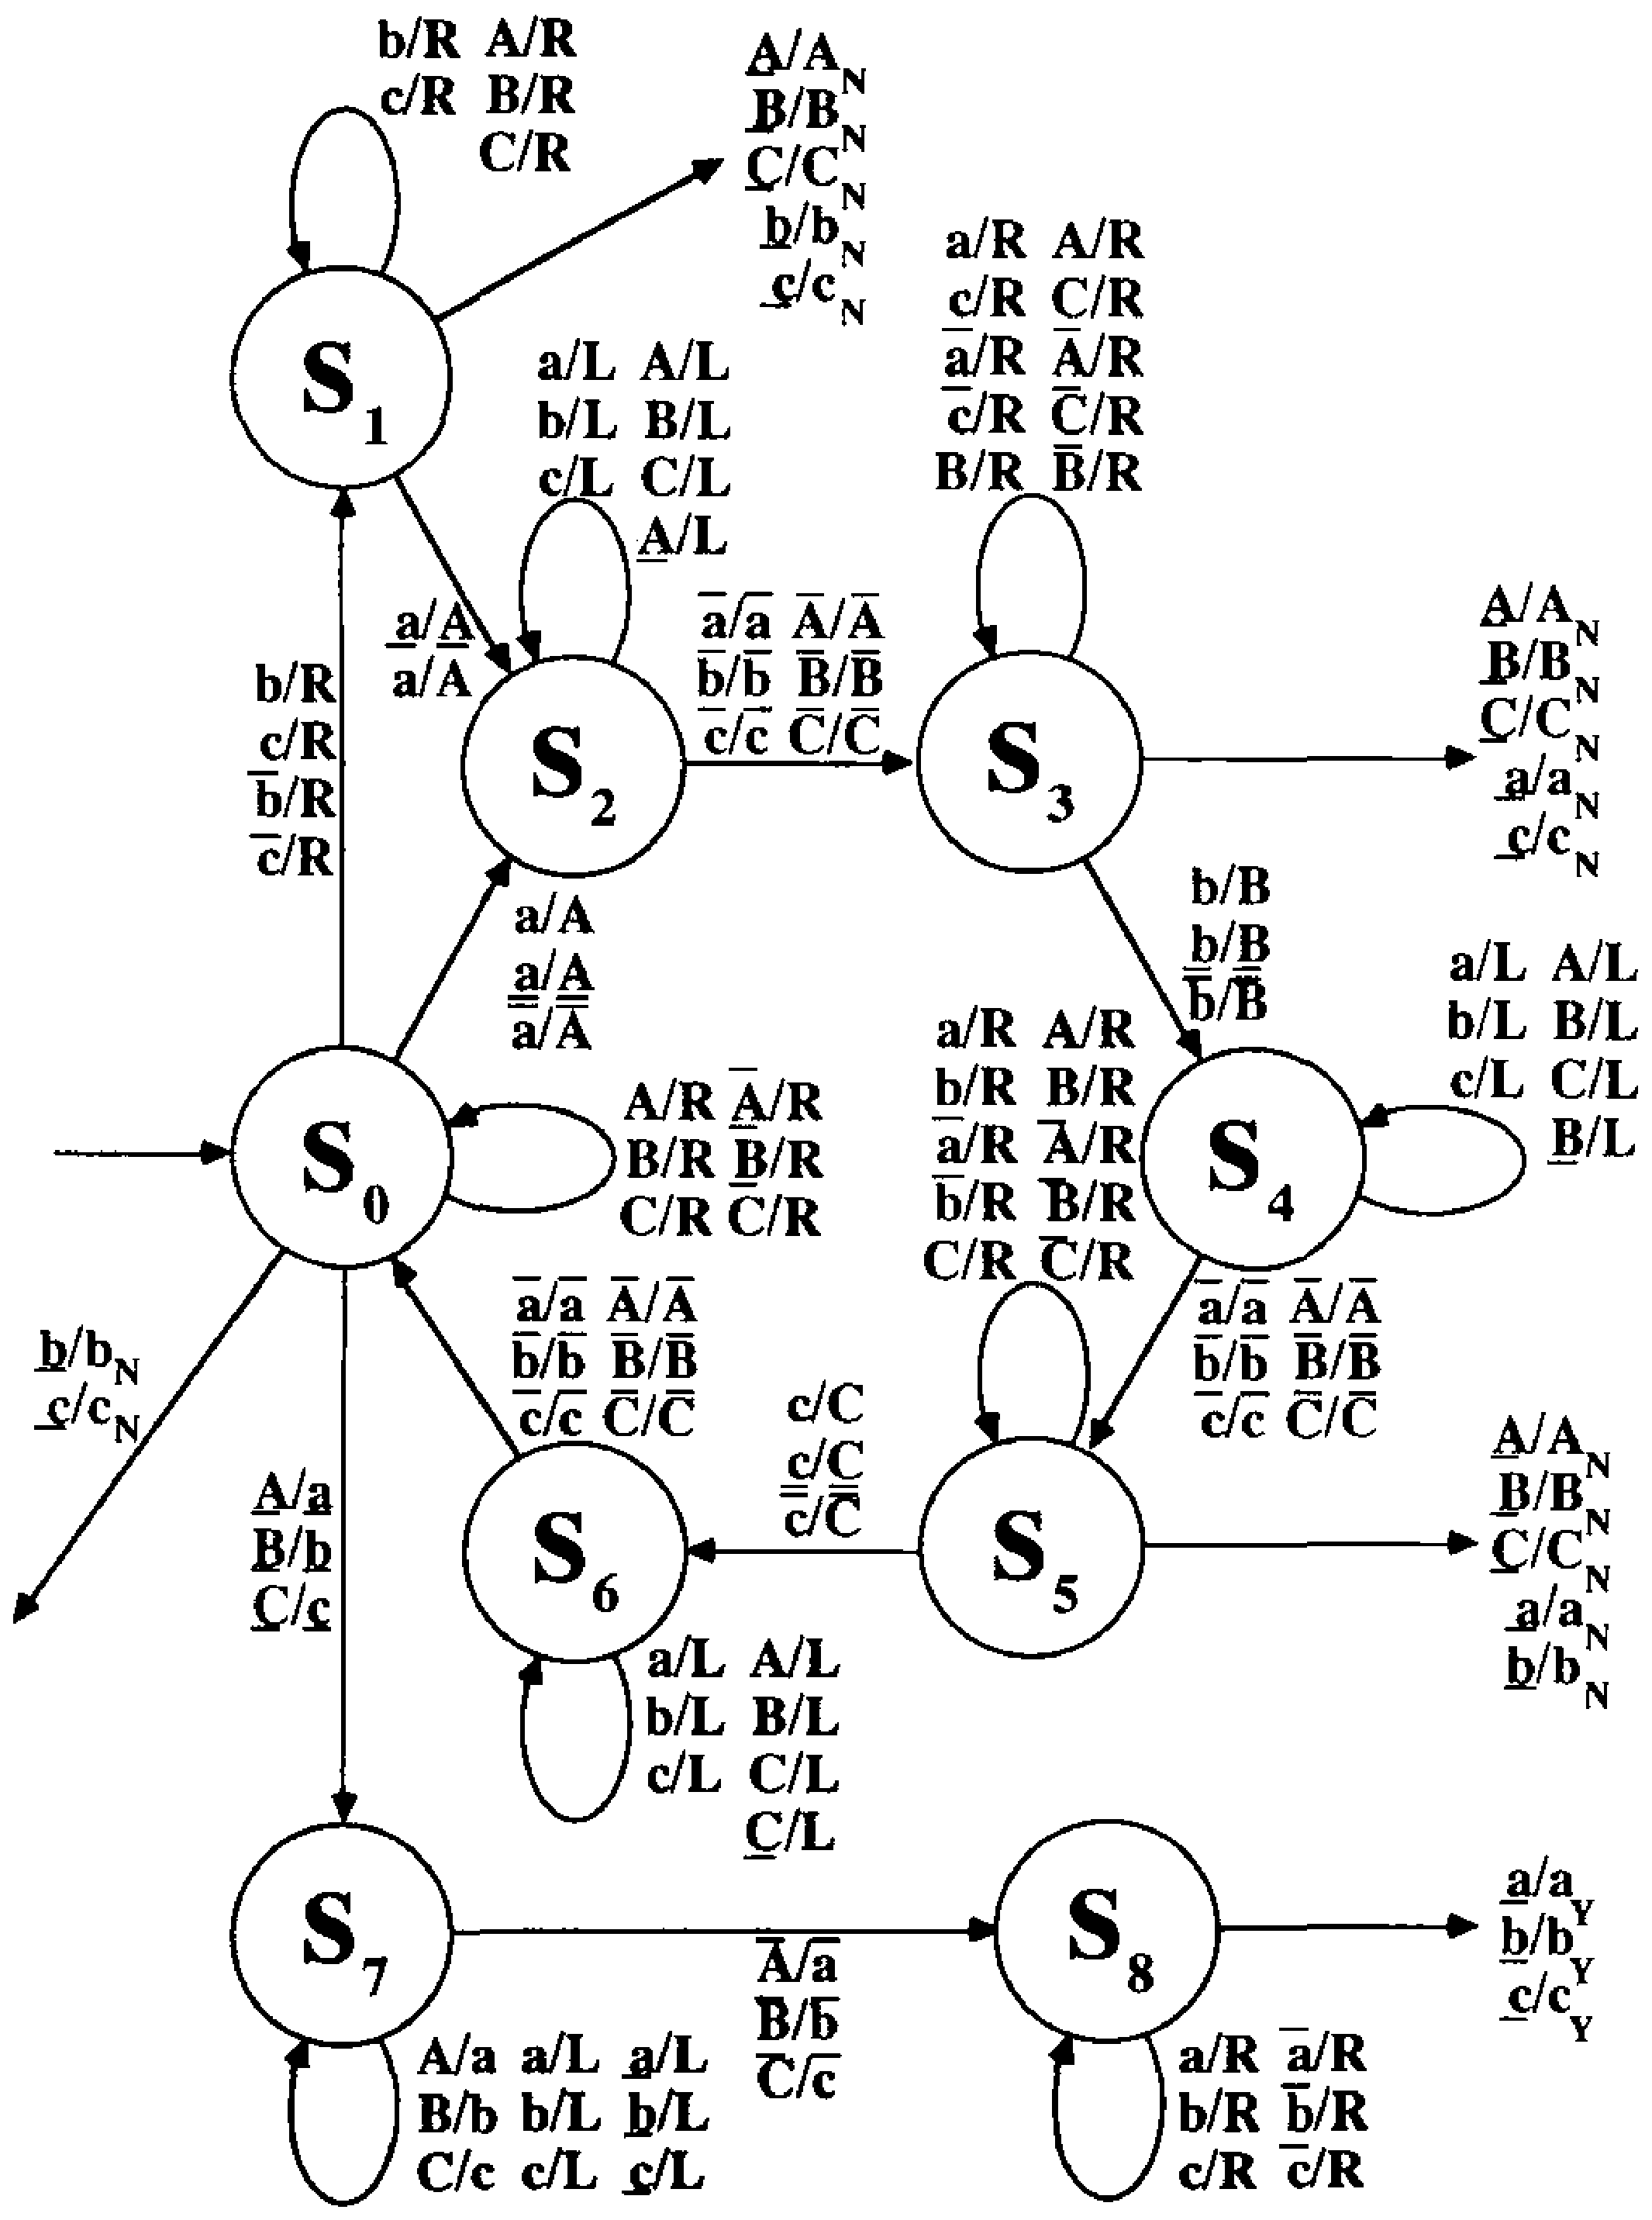
\epsfig{figure=ToFAfigures/fig11-15.eps,height=3.8in}}
\caption{The Turing machine discussed in Example 11.13}\label{fig-11.15}
\end{figure}

% Definition 11.9
\begin{dfn}\label{dfn-11.9}
Given a strict linear bounded automaton
\[ B=\langle\Sigma,\Gamma,\{s_0,s_1,\ldots,s_n\},s_0,\delta\rangle, \]
the context-sensitive grammar corresponding to $B$, $G_B$, is given by
\[ G_B=\langle\Sigma,\Gamma_{\!\!B},Z,P_B\rangle, \]
where $\Gamma_{\!\!B}$ is given by
\[ \Gamma_{\!\!B}=\Gamma\cup\{\pmb{d}_i|\ \pmb{d}\in\Sigma\cup\Gamma,i=1,2,\ldots,n,
	\text{ or }i=\pmb{Y}\}\cup\{Z,S,W\} \]

$P_B$ contains the following classes of productions:
\begin{enumerate}
\item If $\lambda\in L(B)$, then $Z\rightarrow\lambda\in P_B$ \\
$Z\rightarrow S\in P_B$ \\
$(\forall\pmb{d}\in\Sigma)($if $\pmb{d}\in L(B)$, then $S\rightarrow\pmb{d}\in
P_B)$ \\
$(\forall\pmb{d}\in\Sigma)(S\rightarrow W\underline{\pmb{d}}\in P_B)$ \\
$(\forall\pmb{d}\in\Sigma)(W\rightarrow W\pmb{d}\in P_B)$ \\
$(\forall\pmb{d}\in\Sigma)(W\rightarrow\overline{\pmb{d}}_0\in P_B)$
\item Each printing transition gives rise to a production rule as follows:
\[ (\forall s_i,s_j\in S)(\forall\pmb{a},\pmb{b}\in\Sigma\cup\Gamma)(\text{ if }
	\delta(s_i,\pmb{a})=\langle s_j,\pmb{b}\rangle,\text{ then }\pmb{a}_i
	\rightarrow\pmb{b}_j\in P_B) \]
Each move right gives rise to a production rule as follows:
\[ (\forall s_i,s_j\in S)(\forall\pmb{a}\in\Sigma\cup\Gamma)(\text{if }\delta(
	s_i,\pmb{a}) = \langle s_j,\pmb{R}\rangle,\text{ then }(\forall\pmb{d}
	\in\Sigma\cup\Gamma)(\pmb{a}_i\pmb{d}\rightarrow\pmb{ad}_j\in P_B)) \]
Each move left gives rise to a production rule as follows:
\[ (\forall s_i,s_j\in S)(\forall\pmb{a}\in\Sigma\cup\Gamma)(\text{if }\delta(
	s_i,\pmb{a})=\langle s_j,\pmb{L}\rangle,\text{ then }(\forall\pmb{d}\in
	\Sigma\cup\Gamma)(\pmb{da}_i\rightarrow\pmb{d}_j\pmb{a}\in P_B)) \]
Each halt with acceptance gives rise to a production rule as follows:
\[ (\forall s_i\in S)(\forall\pmb{b}\in\Sigma\cup\Gamma)(\forall\pmb{a}\in\Sigma)
	(\text{if }\delta(s_i,\pmb{b})=\langle h,\pmb{a}_{\pmb{Y}}\rangle,
	\text{ then }\pmb{b}_i\rightarrow\pmb{a}_{\pmb{Y}}\in P_B) \]
\item $(\forall\pmb{a},\pmb{b}\in\Sigma)(\pmb{ba}_{\pmb{Y}}\rightarrow\pmb{b}_{
	\pmb{Y}}\pmb{a}\in P_B)$ \\
$(\forall\pmb{a},\pmb{b}\in\Sigma)(\overline{\pmb{b}}\pmb{a}_{\pmb{Y}}\rightarrow
	\pmb{ba}\in P_B)$
\end{enumerate}
\end{dfn}

\subsection*{Example 11.14}

Consider again the strict linear bounded automaton $B$ given in Figure \ref{fig-11.15} and
the corresponding context-sensitive grammar $G_B$. The following derivation
sequences show that $\pmb{babcca}\in L(G_B)$:
\[ Z\Rightarrow S\Rightarrow W\underline{\pmb{a}}\Rightarrow W\pmb{c}\underline{\pmb{a}}
	\Rightarrow W\pmb{cc}\underline{\pmb{a}}\Rightarrow W\pmb{bcc}\underline{\pmb{a}}
	\Rightarrow W\pmb{abcc}\underline{\pmb{a}}\Rightarrow\overline{\pmb{b}}_0
	\pmb{abcc}\underline{\pmb{a}} \]
At this point, only the class 2 productions can be employed, yielding:
\begin{center}\begin{tabular}{r@{ }l@{ }l@{ }l@{ }l}
$\overline{\pmb{b}}_0\pmb{abcc}\underline{\pmb{a}}$ & $\Rightarrow\overline{\pmb{b}}\pmb{a}
	_1\pmb{bcc}\underline{\pmb{a}}$ & $\Rightarrow\overline{\pmb{b}}\pmb{A}_2\pmb{bcc}
	\underline{\pmb{a}}$ & $\Rightarrow\overline{\pmb{b}}_2\pmb{Abcc}\underline{\pmb{a}}$ &
	$\Rightarrow$ \\
& $\ \ \ \ \ \overline{\pmb{b}}_3\pmb{Abcc}\underline{\pmb{a}}$ & $\Rightarrow
	\overline{\pmb{B}}_4\pmb{Abcc}\underline{\pmb{a}}$ && $\Rightarrow$ \\
$\overline{\pmb{B}}_5\pmb{Abcc}\underline{\pmb{a}}$ & $\Rightarrow\overline{\pmb{B}}
	\pmb{A}_5\pmb{bcc}\underline{\pmb{a}}$ & $\Rightarrow\overline{\pmb{B}}\pmb{Ab}_5\pmb{cc}
	\underline{\pmb{a}}$ & $\Rightarrow\overline{\pmb{B}}\pmb{Abc}_5\pmb{c}\underline{\pmb{a}}$
	& $\Rightarrow$ \\
$\overline{\pmb{B}}\pmb{AbC}_6\pmb{c}\underline{\pmb{a}}$ & $\Rightarrow\overline{\pmb{B}}\pmb{Ab}
	_6\pmb{Cc}\underline{\pmb{a}}$ & $\Rightarrow\overline{\pmb{B}}\pmb{A}_6\pmb{bCc}
	\underline{\pmb{a}}$ & $\Rightarrow\overline{\pmb{B}}_6\pmb{AbCc}\underline{\pmb{a}}$
	& $\Rightarrow$ \\
& $\ \ \ \ \ \overline{\pmb{B}}_0\pmb{AbCc}\underline{\pmb{a}}$ & $\Rightarrow
	\overline{\pmb{B}}\pmb{A}_0\pmb{bCc}\underline{\pmb{a}}$ & $\Rightarrow\overline{\pmb{B}}
	\pmb{Ab}_0\pmb{Cc}\underline{\pmb{a}}$ & $\Rightarrow$ \\
$\overline{\pmb{B}}\pmb{AbC}_1\pmb{c}\underline{\pmb{a}}$ && $\DRightarrow\overline{\pmb{B}}
	_2\pmb{AbCc}\underline{\pmb{A}}$ && $\DRightarrow$ \\
$\overline{\pmb{B}}\pmb{Ab}_3\pmb{Cc}\underline{\pmb{A}}$ && $\DRightarrow\overline{\pmb{B}}
	_4\pmb{ABCc}\underline{\pmb{A}}$ && $\DRightarrow$ \\
$\overline{\pmb{B}}\pmb{ABCc}_5\underline{\pmb{A}}$ && $\DRightarrow\overline{\pmb{B}}
	_6\pmb{ABCC}\underline{\pmb{A}}$ && $\DRightarrow$ \\
& $\ \ \ \ \ \overline{\pmb{B}}\pmb{ABCC}\underline{\pmb{A}}_0$ & $\Rightarrow
	\overline{\pmb{B}}\pmb{ABCC}\underline{\pmb{a}}_7$ & $\Rightarrow\overline{\pmb{B}}\pmb{ABCC}_7
	\underline{\pmb{a}}$ & $\Rightarrow$ \\
$\overline{\pmb{B}}\pmb{ABCc}_7\underline{\pmb{a}}$ && $\DRightarrow\overline{\pmb{B}}
	_7\pmb{abcc}\underline{\pmb{a}}$ && $\Rightarrow$ \\
$\overline{\pmb{b}}_8\pmb{abcc}\underline{\pmb{a}}$ & $\Rightarrow\overline{\pmb{b}}\pmb{a}
	_8\pmb{bcc}\underline{\pmb{a}}$ & $\DRightarrow\overline{\pmb{b}}\pmb{abcc}
	\underline{\pmb{a}}_8$
\end{tabular}\end{center}
Finally, since $\delta(s_8,\underline{\pmb{a}})=\langle h,\pmb{a_Y}\rangle$,
the class 3 productions can then be applied:
\[ \overline{\pmb{b}}\pmb{abcc}\underline{\pmb{a}}_8\Rightarrow\overline{\pmb{b}}\pmb{abcca_Y}
	\Rightarrow\overline{\pmb{b}}\pmb{abcc_Ya}\Rightarrow\overline{\pmb{b}}\pmb{abc_Yca}
	\Rightarrow\overline{\pmb{b}}\pmb{ab_Ycca}\Rightarrow\overline{\pmb{b}}\pmb{a_Ybcca}
	\Rightarrow\pmb{babcca} \]

Once again, the grammars springing from Definition \ref{dfn-11.9} can generate sentential
forms corresponding to any string in $\Sigma^*$, as long as the length of the
string is at least two. As with the grammars arising from Definition \ref{dfn-11.8}, only
strings that would have been accepted by the original machine will lead to a
terminal string. If the productions of this example were applied to the
sentential form $\overline{\pmb{b}}_0\pmb{a}\underline{\pmb{a}}$, at each step there
will be exactly one choice of applicable production, until eventually the form
$\overline{\pmb{B}}\pmb{A}\underline{\pmb{a}}_5$ is obtained. At this step, no production will
apply, and therefore a terminal string cannot be generated from $\overline{\pmb{
b}}_0\pmb{a}\underline{\pmb{a}}$. This correspondence between words accepted by the
machine $B$ and words generated by the context-sensitive grammar $G_B$
given in Definition \ref{dfn-11.9} is the foundation of the following theorem.

% Theorem 11.5
\begin{thm}\label{thm-11.5}
Let $\Sigma$ be an alphabet. Then $\LSIG\subseteq\OSIG$. That is, every linear
bounded language can be generated by a type 1 grammar.

\emph{Proof.} Any linear bounded language can be recognized by a strict linear
bounded automaton (see the exercises). Hence, if $L$ is a linear bounded
language, there exists a strict linear bounded automaton $B=\langle\Sigma,
\Gamma,\{s_0,s_1,\ldots,s_n\},s_0,\delta\rangle$ which accepts exactly the words
in $L$ by printing $\pmb{Y}$ on the lowest of the three tracks after restoring
the original word to the middle track. We will employ the grammar $G_B$
corresponding to $B$, as given in Definition \ref{dfn-11.9}. Example 11.14 illustrated
that these productions can be used in a manner similar to those of Definition
\ref{dfn-11.8}, and it is easy to justify that they cannot be combined in unexpected ways.
Induction on the length of $x$ will show that by using just the productions in
class 1,
\[ (\forall x\in\Sigma^*)(\forall\pmb{a},\pmb{b}\in\Sigma)(Z\ \DRightarrow
	\overline{\pmb{a}}_0x\underline{\pmb{b}}) \]

The correspondence between sequences of applications of the class 2 productions
and sequences of moves in $B$ follows as in Theorem \ref{thm-11.4}. Due to the myriad
positions that the integer subscript can occupy, and the special cases caused
by the presence of the overbars and underscores, the general induction statement
is quite tedious to state and is left as an exercise. The statement will again
be applied to the special case in which we are interested, as stated below.
\[ (\forall x\in\Sigma^*)(\forall\pmb{a},\pmb{b}\in\Sigma)(s_0\pmb{a}x\pmb{b}
	\Dvdash\pmb{a}xh\pmb{b_Y}\text{\ \ iff\ \ \ \ }\overline{\pmb{a}}_0x
	\underline{\pmb{b}}\ \ \DRightarrow\ \overline{\pmb{a}}x\pmb{b_Y}) \]
A final induction argument will show that $\overline{\pmb{a}}x\pmb{b_Y}
\DRightarrow\pmb{a}x\pmb{b}$. Thus,
\[ (\forall x\in\Sigma^*)(\forall\pmb{a},\pmb{b}\in\Sigma)(s_0\pmb{a}x\pmb{b}
	\Dvdash\pmb{a}xh\pmb{b_Y}\text{\ \ iff\ \ } Z\ \DRightarrow
	\overline{\pmb{a}}_0x\underline{\pmb{b}}\ \ \DRightarrow\overline{\pmb{a}}x
	\pmb{b_Y}\ \DRightarrow\ \pmb{a}x\pmb{b}) \]
This establishes the correspondence between words \emph{of length at least two}
accepted by $B$ and those generated by $G_B$. Definition \ref{dfn-11.9} included specific
productions of the form $Z\rightarrow\lambda$ and $S\rightarrow\pmb{d}$ to
ensure that words of length 0 and 1 also corresponded. This implies that $L(B)=
L(G_B)$, as was to be shown.
\end{thm}

The proof of Theorem \ref{thm-11.5} argues that there exists a context-sensitive grammar
$G_B$ for each strict linear bounded automaton $B$, and it certainly appears
that given an automaton $B$ we can immediately write down all the productions in
$P_B$, as specified by Definition \ref{dfn-11.9}. However, some of the class 1 productions
may cause some trouble. For example, determining whether the production $Z
\rightarrow\lambda$ is included in $P_B$ depends on whether the automaton halts
with $\pmb{Y}$ when presented with a blank tape. In the next chapter, we will
see that even this simple question cannot be effectively answered for arbitrary
Turing machines! That is, it is impossible to find an algorithm that, when
presented with the state diagram of a Turing machine, can reliably determine
whether or not the machine accepts the empty string. It will be shown that any
such proposed algorithm is guaranteed to give the wrong answer for some Turing
machines. Similarly, it now seems that there might be some uncertainty about
which members of $\Sigma$ give rise to productions of the form $S\rightarrow
\pmb{d}$.

The productions specified by Definition \ref{dfn-11.9} were otherwise quite explicit; only
the productions relating to the immediate generation of a single character or
the empty string were in any way questionable. There are only $|\Sigma|+1$ such
productions, and some combination of them has to be the correct set of
productions to include in $P_B$. Thus, as stated in the theorem, we \emph{are}
assured that a context-sensitive grammar does exist, even if we are unclear as
to exactly which of these special productions it should contain.

As will be seen in Chapter \ref{ch-12}, it \emph{is} possible to determine which words
are accepted (and which are rejected) by linear bounded automata. Unlike
unrestricted Turing machines, there is only a finite span of tape upon which
symbols can be placed. Furthermore, there are only a finite number of characters
that can appear in those cells, a finite number of positions the tape head can
be in, and a finite number of states to consider. The limited number of
configurations makes it possible to determine exactly which words of a given
size are recognized by the LBA.

We have seen that every linear bounded automaton is equivalent to a strict
linear bounded automaton, and these have equivalent type 1 grammars. Conversely,
every type 1 grammar generates a linear bounded language, which implies there is
another correspondence between a generative construct and a cognitive construct.

% Corollary 11.2
\begin{cor}\label{cor-11.2}
The class of languages generated by context-sensitive grammars is exactly the
linear bounded languages. That is, $\LSIG=\OSIG$.

\emph{Proof.} The proof follows immediately from Theorems \ref{thm-11.3} and \ref{thm-11.5}.
\end{cor}

\section{Closure Properties and The Hierarchy Theorem}\label{sec-11.4}

Finally, we consider some of the closure properties of the classes of languages
explored in this chapter. Since $\TSIG=\ZSIG$ we may use either cognitive or
generative constructs for this class, whichever is most convenient. The fact
that $\LSIG=\OSIG$, will allow similar freedom for the type 1 languages. The
next theorem illustrates a case in which the grammatical construct is the
easier to use.

% Theorem 11.6
\begin{thm}\label{thm-11.6}
Let $\Sigma$ be an alphabet. Then $\TSIG$, is closed under union.

\emph{Proof.} If $L_1$ and $L_2$ are two Turing-acceptable languages, then by
Theorem \ref{thm-11.4} there are type 0 grammars $G_1=\langle\Omega_1,\Sigma,S_1,P_1
\rangle$ and $G_2=\langle\Omega_2,\Sigma,S_2,P_2\rangle$ that recognize $L_1$
and $L_2$. Without loss of generality, assume that $\Omega_1\cap\Omega_2=
\emptyset$. Choose a new nonterminal $Z$ such that $Z\notin\Omega_1\cup\Omega_2$,
and consider the new type 0 grammar $G^{\cup}$ defined by $G^{\cup}=\langle
\Omega_1\cup\Omega_2\cup\{Z\},\Sigma,Z,P_1\cup P_2\cup\{Z\rightarrow S_1,Z
\rightarrow S_2\}\rangle$. Clearly, $L(G^{\cup})=L(G_1)\cup L(G_2)$. By Theorem
\ref{thm-11.2}, there is a Turing machine equivalent to $G^{\cup}$, and hence $L_1\cup
L_2$ is Turing acceptable.
\end{thm}

Theorem \ref{thm-11.6} could be proved directly by constructing a new Turing machine
from Turing machines $T_1$ and $T_2$ accepting $L_1$ and $L_2$. It is a bit
harder to give a concrete proof and care must be taken to avoid inappropriate
constructions. For example, it would be incorrect to build the new machine in
such a way that it first simulates $T_1$ halting with $\pmb{Y}$ if $T_1$ does,
and then simulating $T_2$ if $T_1$ would have halted with $\pmb{N}$. It must be
remembered that there is no guarantee that a Turing machine will \emph{ever}
halt for a given word. The above construction will incorrectly reject words that
could be recognized by $T_2$ but which were rejected by $T_1$ because $T_1$
never halted; the new machine would never get a chance to simulate $T_2$. One
valid construction involves a two-tape Turing machine, which immediately copies
the input word onto the second tape. By using a \Index{cross product} of the states of
$T_1$ and $T_2$ and appropriate transitions, the action of both machines
could be simultaneously simulated, and the new machine would accept as soon as
either simulation indicated that the word should be accepted. A slight
modification of this construct would show that \TSIG\ is also closed under
intersection, but the next theorem outlines a superior method.

% Theorem 11.7
\begin{thm}\label{thm-11.7}
Let $\Sigma$ be an alphabet. Then \TSIG\ is closed under intersection.

\emph{Proof.} $L_1$ and $L_2$ are two Turing-acceptable languages recognized by
the Turing machines $T_1$ and $T_2$, respectively. We build a new Turing machine
$T^{\cap}$ with $T_1$ and $T_2$ as submachines. $T^{\cap}$ transfers control to
the submachine $T_1$. If $T_1$ never halts, the input will be rejected, which is
the desired result. If $T_1$ halts, $T^{\cap}$ erases the $\pmb{Y}$ and moves
the tape head back to the leftmost character and transfers control to the
submachine $T_2$. $T^{\cap}$ will halt if $T_2$ does, and if $T_2$ also accepts,
$\pmb{Y}$ will be left in the proper place on the tape. $T^{\cap}$ therefore
accepts if and only if both $T_1$ and $T_2$ accept, and hence $L_1\cap L_2$ is
Turing acceptable.
\end{thm}

Note that it was important that, except for the presence of $\pmb{Y}$ after the
input word, $T_1$ left the tape in the same condition it found it, with the
input string intact for $T_2$. As with type 3 and type 2 grammars, there is no
pleasant way to combine type 0 grammars to produce a grammar that generates the
intersection of type 0 languages, although Theorem \ref{thm-11.7} guarantees (along with Corollary \ref{cor-11.1}) that such a
grammar must surely exist.

% Theorem 11.8
\begin{thm}\label{thm-11.8}
Let $\Sigma$ be an alphabet. Then \TSIG\ is closed under reversal, homomorphism,
inverse homomorphism, substitution, concatenation, and Kleene closure.

\emph{Proof.} The proof for reversal is almost trivial; it is almost as simple
as replacing every transition that moves the tape head to the right with a
transition to the left, and likewise making left moves into right moves. This
will yield a mirror image machine, which when started at the \emph{right}most
character will print $\pmb{Y}$ just past the \emph{left}most character. We
therefore have to modify this machine by adding preliminary states that will
move the tape head from its traditional leftmost starting position to the
opposite end of the word. Similarly, just before the $\pmb{Y}$ would be printed,
we must again move the tape head to the right.

The description of the modifications necessary to convert a type 0 grammar into
one that generates the reverse of the original is even more succinct: Each rule
in the original grammar is modified by writing the characters to the left of the
production symbol $\rightarrow$ backward, and similarly reversing the string on
the right of $\rightarrow$. That is, a production like $\pmb{Dc}\rightarrow
\pmb{ABe}$ would become $\pmb{cD}\rightarrow\pmb{eBA}$. A relatively trivial
induction on the number of steps in a derivation proves that the new grammar
accepts the reverse of the original language. The proofs of closure under the
remaining operators are left for the exercises.
\end{thm}

As shown in Chapter \ref{ch-12}, there are some operators under which \TSIG\ is not
closed. Complementation is perhaps the most glaring exception. The closure
properties of \LSIG\ are very similar to those of \TSIG. In most cases, slight
modifications of the above proofs carry over to the type 1 languages.

% Theorem 11.9
\begin{thm}\label{thm-11.9}
Let $\Sigma$ be an alphabet. Then \OSIG\ is closed under reversal, homomorphism,
inverse homomorphism, substitution, concatenation, union, and intersection.

\emph{Proof.} Both proofs given for reversal carry over without modification. In
the cognitive approach, the states added to the mirror image Turing machine keep
the tape head within the confines of the input word, and hence if the original
machine was a LBA, the new version will also be a LBA. In the generative
approach, reversing the characters in type 1 productions still results in a type
1 grammar. That is, if the original grammar had no contracting productions,
neither will the new grammar.

Proving that the union of two type 1 languages is type 1 is similar to the
proof given in Theorem \ref{thm-11.6}, although care must be taken to avoid extraneous
productions of the form $Z_1\rightarrow\lambda$. Building an intersection
machine from two linear bounded automata can be done exactly as described in
Theorem \ref{thm-11.7}. The remaining closure properties are left for the exercises.
\end{thm}

It is clear from our definitions that $\OSIG\subseteq\ZSIG$, but we have yet to
prove that $\OSIG\subset\ZSIG$. That the inclusion is proper and \ZSIG\ is truly
a larger class than \OSIG\ will be shown to be a consequence of the material
considered in Chapter \ref{ch-12}. Apart from this one missing piece, we have over the
course of several chapters encountered the major components of the following
\emph{hierarchy theorem}\index{hierarchy!of language classes}.

% Theorem 11.10
\begin{thm}\label{thm-11.10}
Let $\Sigma$ be an alphabet for which $\|\Sigma\|\geq 2$. Then
\[ \DSIG=\WSIG=\RSIG=\GSIG\subset\USIG\subset\CSIG=\PSIG\subset\LSIG=\OSIG
	\subset\ZSIG=\TSIG \]

\emph{Proof.} The cognitive power of deterministic and nondeterministic finite
automata was shown to be equivalent in Chapter \ref{ch-4}, and their relation to regular
expressions was investigated in Chapter \ref{ch-6}. These were all shown to describe the
type 3 languages in Chapter \ref{ch-8}. In Chapter \ref{ch-9}, Theorem \ref{thm-9.1} and Corollary \ref{cor-9.1}
showed that the context-free languages (over alphabets with at least two
symbols) properly contained the unambiguous context-free languages, which in
turn properly contained the regular languages. In Chapter \ref{ch-10}, the
(nondeterministic) pushdown automata were shown to recognize exactly the type 2
languages. The context-sensitive language $\{x\in\{\pmb{a},\pmb{b},\pmb{c}\}^*|\ 
\ |x|_{\pmb{a}}=|x|_{\pmb{b}}=|x|_{\pmb{c}}\}$ is not context free, so the type
1 languages properly contain the type 2 languages. In this chapter, the linear
bounded automata were shown to be recognize exactly the type 1 languages and
Turing machines were shown to accept the type 0 languages. Corollary \ref{cor-12.4} will
show that the type 1 languages are properly included in the type 0 languages.
\end{thm}

\section*{Exercises}
\begin{enumerate}[{11.}1.]
\item By making the appropriate analogies for states and input, answer the
musical question ``How is a Turing machine like an elevator?'' What essential
(missing) component prevents an elevator from modeling a general computing
device?

\item Let $\Sigma=\{\pmb{a},\pmb{b},\pmb{c}\}$ and let $L=\{w\ |\ w=w^r\}$.
\begin{enumerate}
\item Explicitly define a deterministic, one-tape, one-head Turing machine that
will recognize $L$.
\item Justify that there exists a linear bounded automaton that accepts $L$.
\item Describe how nondeterminism or additional tapes and heads might be
employed to recognize $L$.
\end{enumerate}

\item Let $\Sigma=\{\pmb{a}\}$. Explicitly define a deterministic, one-tape,
one-head Turing machine that will recognize $\{\pmb{a}^n\ |\ n$ is a perfect
square$\}$.

\item Let $\Sigma=\{\pmb{a},\pmb{b},\pmb{c}\}$.
\begin{enumerate}
\item Explicitly define a deterministic, one-tape, one-head Turing machine that
will recognize\linebreak $\{\pmb{a}^k\pmb{b}^n\pmb{c}^m\ |\ \ (k\not= n)\wedge(n\not= m)\}$.
\item Explicitly define a deterministic, one-tape, one-head Turing machine that
will recognize $\{x\in\{\pmb{a},\pmb{b},\pmb{c}\}^*|\ \ |x|_{\pmb{a}}\not=|x|_{
\pmb{b}}\wedge |x|_{\pmb{b}}\not=|x|_{\pmb{c}}\}$.
\end{enumerate}

\item \begin{enumerate}
\item Recall that there are several common definitions of acceptance that
can be applied to Turing machines. Design a machine $M$ for which
\[ L(M)=L_1(M)=L_2(M)=L_3(M)=\{x\in\{\pmb{a},\pmb{b},\pmb{c}\}^*|\ \ |x|_{\pmb{a}}
	=|x|_{\pmb{b}}=|x|_{\pmb{c}}\}. \]
\item For any Turing-acceptable language $L$, is it always possible to find a
corresponding machine for which $L(M)=L_1(M)=L_2(M)=L_3(M)=L$? Justify your
answer.
\end{enumerate}

\item Let $L=\{ww\ |\ w\in\{\pmb{a},\pmb{b},\pmb{c}\}^*\}$.
\begin{enumerate}
\item Explicitly define a deterministic, one-tape, one-head Turing machine that
will recognize $L$.
\item Justify that there exists a linear bounded automaton that accepts $L$.
\item Describe how nondeterminism or additional tapes and heads might be
employed to recognize $L$.
\end{enumerate}

\item Given an alphabet $\Sigma=\{\pmb{a}_1,\pmb{a}_2,\pmb{a}_3,\ldots,\pmb{a}_n\}$,
associate each word with the base $n$ number derived from the subscripts. Thus,
$\pmb{a}_3\pmb{a}_2\pmb{a}_4$ is associated with 324, $\pmb{a}_1$ with 1,
and $\lambda$ with 0. These associated numbers then imply a \emph{lexicographic}
ordering of $\Sigma^*$, with
\[ \lambda<\pmb{a}_1<\pmb{a}_2<\pmb{a}_3<\cdots<\pmb{a}_1\pmb{a}_1<\pmb{a}_1
	\pmb{a}_2<\pmb{a}_1\pmb{a}_3<\cdots<\pmb{a}_2\pmb{a}_1<\pmb{a}_2
	\pmb{a}_2<\cdots<\pmb{a}_1\pmb{a}_1\pmb{a}_1<\cdots \]
\begin{enumerate}
\item Given an alphabet $\Sigma$, build a Turing machine that, given an input
word $x$, will replace that word with the string that follows $x$ in
lexicographic order.
\item Using the machine in part (a) as a submachine, build a Turing machine that
will start with a blank tape and sequentially generate the words in $\Sigma^*$
in lexicographic order, erasing the previous word as the following word is
generated.
\item Using the machine in part (a) as a submachine, build a Turing machine that
will start with a blank tape and sequentially enumerate the words in $\Sigma^*$
in lexicographic order, placing each successive word to the right of the
previous word on the tape, separated by a blank.
\item Explain how these techniques can be used in building a deterministic
version of a nondeterministic Turing machine.
\end{enumerate}

\item Define a \emph{\Index{semi-infinite tape}} as one that has a distinct left
boundary but extends indefinitely to the right, such as those employed by DFAs.
\begin{enumerate}
\item Given a Turing machine satisfying Definition \ref{dfn-11.1}, define an equivalent
two-track Turing machine with a semi-infinite tape.
\item Prove that your construction is equivalent to the original.
\end{enumerate}

\item Let $\Sigma=\{\pmb{a}\}$. Explicitly define a deterministic, one-tape,
one-head Turing machine that will recognize $\{\pmb{a}^n\ |\ n$ is a power of 2$\}=
\{\pmb{a},\pmb{aa},\pmb{aaaa},\ldots\}$.

\item Define a three-head Turing machine that accepts $\{x\in\{\pmb{a},\pmb{b},
\pmb{c}\}^*|\ \ |x|_{\pmb{a}}=|x|_{\pmb{b}}=|x|_{\pmb{c}}\}$. Assume that all
three heads start on the leftmost character. Is there any need for any of the
heads to ever move left?

\item Let $\Sigma$ be an alphabet. Prove that every context-free language is
Turing-acceptable by providing the details for the construction discussed in
Lemma \ref{lmm-11.1}.

\item Let $\Sigma$ be an alphabet. Prove that every type 1 language is a LBL by
providing the details for the construction discussed in Theorem \ref{thm-11.3}.

\item Let $M=\langle\Sigma,\Gamma,S,s_0,\delta\rangle$ be a linear bounded
automaton. Show how to convert $M$ into a three-track automaton that never scans
any cells but those containing the original word by:
\begin{enumerate}
\item Explicitly defining the new alphabets.
\item Explicitly defining the new transitions from the old. (\emph{Hint:} From
any state, an old transition ``leaving'' the word to scan one of the delimiters
must return to the word in a unique manner.)
\item Prove that for words of length at least 2 your new strict linear bounded
automaton accepts exactly when $M$ does.
\end{enumerate}

\item By adding appropriate new symbols (of the form $\overline{\underline{\pmb{
b}}})$ and suitable transitions:
\begin{enumerate}
\item Modify the strict linear bounded automaton defined in Exercise 11.13 so
that it correctly handles strings of length 1.
\item Assume that a strict LBA that initially scans a blank is actually scanning
an empty tape. If we expect to handle the empty string, we cannot insist that a
strict linear bounded automaton never scan a cell that is not part of the input
string, since the tape head must initially look at something. If we instead
require that the tape head of a strict LBA may never \emph{actively move to} a
cell that is not part of the input string, then the dilemma is solved. Show that
such a strict LBA can be found for any type 1 language.
\end{enumerate}

\item Refer to Theorem \ref{thm-11.4} and show, by inducting on the number of transitions,
that
\begin{center}\begin{tabular}{l}
$(\forall s,t\in S\cup\{h\})(\forall\alpha,\beta,\gamma,\omega\in(\Sigma\cup
\Gamma)^*)$ \\
$(\alpha s\beta\Dvdash\gamma t\omega\text{\ \ iff\ \ }(\exists i,j,m,n\in\NN)
([\pmb{\#}^i\alpha s\beta\pmb{\#}^j]\DRightarrow[\pmb{\#}^m\gamma t\omega
\pmb{\#}^n]))$
\end{tabular}\end{center}

\item State and prove the general induction statement needed to rigorously
prove Theorem \ref{thm-11.5}.

\item If $G=\langle\Sigma,\Gamma,Z,P\rangle$ is a grammar for a type 0 language:
\begin{enumerate}
\item Explain why the following construction may not accept $L(G)^*$: Choose a
new start symbol $W$, and form $G_{\pmb{*}}=\langle\Sigma,\Gamma\cup\{W\},W,
P\cup\{W\rightarrow\lambda,W\rightarrow WW,W\rightarrow Z\}\rangle$.
\item Give an example of a grammar that illustrates this flaw.
\item Given a type 0 grammar $G=\langle\Sigma,\Gamma,Z,P\rangle$, define an
appropriate grammar $G_{\pmb{*}}$ that should accept the Kleene closure of
$L(G)$.
\item Prove that the construction defined in part (c) has the property that
$L(G_{\pmb{*}})=L(G)^*$.
\end{enumerate}

\item Let $\Sigma$ be an alphabet. Prove that \TSIG\ is closed under:
\begin{enumerate}
\item Homomorphism
\item Inverse homomorphism
\item Concatenation
\item Substitution
\end{enumerate}

\item \begin{enumerate}
\item Show that any Turing machine $A_1$ accepting $L=L_1(A_1)$ has an
equivalent Turing machine $A_2$ for which $L=L_2(A_2)$ by explicitly modifying
the quintuple for $A_1$ and proving that your construction behaves as desired.
\item Show that any Turing machine $A_2$ accepting $L=L_2(A_2)$ has an
equivalent Turing machine $A_3$ for which $L=L_3(A_3)$ by explicitly modifying
the quintuple for $A_2$ and proving that your construction behaves as desired.
\end{enumerate}

\item Let $\Sigma$ be an alphabet. Prove that \OSIG\ is closed under:
\begin{enumerate}
\item Homomorphism
\item Inverse homomorphism
\item Concatenation
\item Substitution
\end{enumerate}
\end{enumerate}

\chapter{Decidability}\label{ch-12}

In this chapter, the nature and limitations of algorithms are
explored. We will first look at the general properties that can be
ascertained about finite automata and FAD languages. For example,
we might like to be able to enter the state transition table of a
DFA into a suitably sized array and then run a program that determines
whether the DFA was connected. An algorithm for checking this
property was outlined in Chapter \ref{ch-3}. Similarly, we have seen that
it is possible to write a program to check whether an arbitrary DFA
is minimal. We know this property can be reliably checked because
we proved that the algorithms in Chapter 3 could be applied to
ascertain the correct answer for virtually every conceivable DFA.
There are an infinite number of DFAs about which the question can
be posed, and yet our algorithm decides the question correctly in
all cases. In the following section we consider questions that can
be asked about more complex languages and machines.

%
% Do not forget to fix up all references to sections and chapters using
% label and ref (this is important for the index).
%

In the latter part of this chapter, we will see that unlike the questions in
Sections \ref{sec-12.1} and \ref{sec-12.2}, there are some questions that are in
a fundamental sense unanswerable in the general case. That is, there cannot
exist an algorithm that correctly answers such a question in all cases. These
questions will be called undecidable. An undecidable question about Pascal
programs is considered in detail in Section \ref{sec-12.3} and is independent of
advanced machine theory. The concept of undecidability is addressed formally in
Section \ref{sec-12.4}, and other undecidable problems are also presented.

% 12.1 DECIDABLE QUESTIONS ABOUT REGULAR LANGUAGES
\section{Decidable Questions About Regular Languages}\label{sec-12.1}

Recall that a procedure is a finite set of instructions that
unambiguously specifies deterministic, discrete steps for performing
some task. In this chapter, the task will generally involve providing
the correct answer to some yes-no question. Most questions that
involve a numerical answer can be rephrased as a yes-no question
of similar complexity. For example, the question ``What is the minimum
number of states necessary for a DFA to accept the language represented
by the regular expression $R$?'' has the yes-no analog ``Does there
exist a DFA with fewer than, say, five states that accepts the
language represented by the regular expression $R$?'' Clearly, if we
can answer the first question, the second question is easy to answer.
Conversely, if questions like the second one can be answered for
any number we wish (rather than just five), then the answer to the
first question can be deduced.

Recall also that an \Index{algorithm} is a procedure that is guaranteed to halt in all
instances. Note that ``guaranteed to halt'' does not mean that there is a fixed
time limit on how long it may take to finish the procedure for all inputs; some
instances may take far longer than others. For example, the question ``Does
there exist a DFA with fewer than ten states that accepts the language
represented by $\pmb{ab}(\pmb{b}\cup\pmb{c})^*$?'' will probably take less time
to answer than ``Does there exist a DFA with fewer than ten states that accepts
the language represented by $\pmb{a}^*\pmb{b}((\pmb{b}^*\pmb{d}\cup\pmb{c}^*
\pmb{b})\pmb{d}\cup\pmb{e})^*?$''

It is important to keep in mind that algorithms are intended to provide a
general solution to a vast array of similar problems and are (usually) not
limited to a single specific instance. As an example, consider the task of
sorting a file containing the three names:
\begin{quote}
Williams \\
Jones \\
Smith
\end{quote}
A variety of sorting algorithms, when applied to this file, will produce the
correct output. It is also possible to write a program that ignores its input
and always prints the lines
\begin{quote}
Jones \\
Smith \\
Williams
\end{quote}
This program does yield the correct answer for the particular problem we wished
to solve, and indeed it solves the sorting problem for all files that contain
exactly these three particular names in some arbitrary order (there are six such
files). Thus, this trivial program is an algorithm that solves the sorting
problem for these six specific instances. A slightly more complex program might
be capable of printing two or three distinct answers, depending on the input,
and thus solve the sorting problem for an even larger (but still finite) class
of instances.

It should be clear that producing an algorithm that solves a finite set of
instances is no great accomplishment, since these algorithms are guaranteed to
exist. Such an algorithm could be programmed as one big case statement, which
identifies the particular input instance and produces the corresponding output
for that instance. Algorithms that apply to an infinite set of instances are of
much more theoretical and practical interest.

% Definition 12.1
\begin{dfn}\label{dfn-12.1}\index{instance of a question}
Given a set of \emph{instances} and a yes-no \emph{question} that can be
applied to those instances, we will say that the question is
\emph{\Index{decidable}} if there is an algorithm for determining in each
instance the (correct) answer to the question.
\end{dfn}

A more precise definition of decidability is presented in Section \ref{sec-12.4}, based
on the perceived relationship between Turing machines and algorithms. As
mentioned earlier, if the set of instances is finite, an algorithm is guaranteed
to exist, no matter how complex the question appears to be.

\subsection*{Example 12.1}\label{ex-12.1}

A typical set of instances might be the set of all deterministic finite
automata over a given alphabet $\Sigma$; a typical question might be whether a
given automaton accepts at least one string in $\Sigma^*$.

It is possible to devise an algorithm to correctly answer the question posed
in Example \ref{ex-12.1} for every finite automaton $A=\langle\Sigma,S,s_0,\delta,F\rangle$.
The first idea that might come to mind is to simply look at strings from
$\Sigma^*$ in an orderly manner and use $\DBAR$ to determine whether that string
is accepted by $A$; if we find a string that does reach a final state, it is
clear that the answer to the question should be ``YES$-L(A)\not=\emptyset$,''
while if we never find a string that is accepted, the answer should be ``NO$-
L(A)=\emptyset$.'' This procedure is guaranteed to halt and give the correct
answer if the language is indeed nonempty. However, the procedure will never
halt and answer NO (in a finite amount of time) because there are an infinite
number of strings in $\Sigma^*$ that must be checked. A modification of this
basic idea is necessary to produce a procedure that will halt under all
circumstances (that is, to produce an algorithm ).

% Theorem 12.1
\begin{thm}\label{thm-12.1}
Given any alphabet $\Sigma$ and a DFA $A=\langle\Sigma,S,s_0,\delta,F\rangle$,
it is decidable whether $L(A)=\emptyset$.

\emph{Proof.} Let $n=\|S\|$. Since both $\Sigma$ and $S$ are finite sets,
\[ B = \{\lambda\}\cup\Sigma\cup\Sigma^2\cup\cdots\cup\Sigma^{n-1} \]
is a finite set, and we can examine each string of this set and still have a
procedure that halts. There is clearly an algorithm for determining the set $C$
of all states that are reached by these few strings. Specifically,
\[ C=\{\DBAR(s_0,x)\ |\ x\in\Sigma^*\wedge |x|<n\}=\{\DBAR(s_0,x)|x\in B\}. \]
Note that Theorem \ref{thm-2.7} implies that if a string (of \emph{any} length) is
accepted by $A$ then there is another string of length less than $n$ that is
also accepted by $A$. Consequently, it is sufficient to examine only the
``short'' strings contained in $B$ rather than examine all of $\Sigma^*$. If any
of the strings in $B$ lead to a final state (that is, if $C\cap F\not=\emptyset$),
then the answer to the question is clearly ``NO$-L(A)$ is \emph{not} empty,''
while if $C\cap F=\emptyset$, then Theorem \ref{thm-2.7} guarantees that ``YES$-L(A)$
\emph{is} empty'' is the correct answer. We have therefore constructed an
algorithm (which computes $C$ and then examines $C\cap F$, both of which can be
done in a finite amount of time) for determining whether the language accepted
by a given machine is empty.
\end{thm}

The definition of $C$ does not suggest the most efficient algorithm for
calculating the set $C$; better strategies are available. The technique is
similar to that employed to find the state equivalence relation $E_A$. $C$ is
actually the set of connected states $S^c$, which can be calculated recursively
as indicated in Definition \ref{dfn-3.10}. Note that Theorem \ref{thm-12.1} answers the question
posed in Example \ref{ex-12.1}. The set of instances to which this question applies can
easily be expanded. It can be shown that it is decidable whether $L(A)=\emptyset$
for any NDFA $A$ by first employing Definition \ref{dfn-4.5} to find the equivalent DFA
$A^d$ and then applying the method outlined in Theorem \ref{thm-12.1} to that machine. It
is possible to find a much more efficient algorithm for answering this question
that does not rely on the conversion to a DFA (see the exercises).

Just as the algorithm for converting an NDFA into a DFA allows the emptiness
question to be answered for NDFAs, the techniques in Chapter 6 justify that
the similar question for regular expressions is decidable. That is, since
every regular expression has an equivalent DFA, the question of whether a
regular expression describes any strings is clearly decidable. Similar
extensions can be applied to most of the results in this section. Just as we can
decide whether a DFA $A$ accepts any strings, we can also decide if $A$ accepts
an infinity of strings, as shown by Theorem \ref{thm-12.2}. This can be proved by a
related appeal to Theorem \ref{thm-12.1}, but an efficient algorithm for answering this
question depends on the following lemma.

% Lemma 12.1
\begin{lmm}\label{lmm-12.1}
Let $\Sigma$ be an alphabet, $A=\langle\Sigma,S,s_0,\delta,F\rangle$ be a finite
automaton, $n=\|S\|$, and $M=\{x\ |\ x\in L(A)\wedge |x|\geq n\}$. Then, if $M\not=
\emptyset$, $M$ must contain a string of minimal length (call it $x_m$), and
furthermore $|x_m| < 2n$.

\emph{Proof.} The proof is obtained by repeated application of the pumping lemma
with $i=0$ (see the exercises and Theorem \ref{thm-2.7}).
\end{lmm}

A question similar to the one posed in Theorem \ref{thm-12.1} is ``Does a given DFA
accept a finite or an infinite number of strings?'' This is also a decidable
question, as demonstrated by the following theorem. The proof is based on the
observation that a DFA $A$ that accepts no strings of length greater than some
fixed constant must by definition recognize a finite set, while the pumping
lemma implies that if $L(A)$ contains a sufficiently long string, then $L(A)$
must contain an infinite number of related strings.

% Theorem 12.2
\begin{thm}\label{thm-12.2}
Given any alphabet $\Sigma$ and a DFA $A=\langle\Sigma,S,s_0,\delta,F\rangle$,
it is decidable whether $L(A)$ is an infinite set.

\emph{Proof.} Let $n=\|S\|$. Clearly, if $A$ accepts no strings of length $n$ or
greater, then L(A) is finite. From the pumping lemma, we know that if $A$
accepts even one string of length equal to or greater than $n$, then $A$ must
accept an infinite number of strings. We still cannot check all the strings of
length greater than $n$ and have a procedure that halts, so Lemma \ref{lmm-12.1} will be
invoked to argue that if a long string is accepted by $A$, then a string whose
length is in the range $n\leq |x| < 2n$ must be accepted, and it is therefore
sufficient to check the strings in this limited range. Thus, our algorithm will
consist of computing the intersection of $\{\delta(s_0,y)\ |\ y\in\Sigma^*\wedge n
\leq |y| < 2n\}$ and $F$. $L(A)$ is infinite iff this intersection is
nonempty.
\end{thm}

If we were to write a program that consulted the matrix containing the state
transition table for $A$ to actually determine $\{\delta(s_0,y)\ |\ y\in\Sigma^*
\wedge n\leq |y| < 2n\}$, it would be very inefficient to implement this
computation as implied by the definition. Repeatedly looking up entries in the
state transition table to determine \DBAR\ for each word in this large class of
specified strings would involve an enormous duplication of effort. It is far
better to recursively calculate $R_i=\{\DBAR(s_0,x)\ |\ x\in \Sigma^i\}$, which
represents the set of all states that can be reached by strings of length
exactly $i$. This can be easily computed by defining $R_0=\{s_0\}$ and using the
recursive formula
\[ R_{i+1}= R_i \cup \{\delta(s,\pmb{a})\ |\ \pmb{a}\in\Sigma,s\in R_i\} \]
Successive sets can thereby be calculated from $R_0$. When $R_i$ is reached, it
is checked against $F$, and the algorithm halts and returns Yes if they have a
common state. Otherwise, $R_{n+1}$ through $R_{2n-1}$ are checked, and No is
returned if no final state appears in these groups. This method is easily
adaptable to nondeterministic finite automata by setting $R_0$ to be the set of
all start states and adjusting the definition of $R_{i+1}$ to conform to NDFA
notation.

The involved arguments presented in Lemma \ref{lmm-12.1} and the proof of
Theorem \ref{thm-12.2} are necessary to justify that the above efficient
recursive algorithm correctly answers the question of whether a finite automaton
accepts an infinite number of strings. However, if we were simply interested in
justifying that it is decidable whether $L(A)$ is infinite, without worrying about efficiency, it would have been
much more convenient to simply adapt the result of Theorem \ref{thm-12.1}. In
particular, we could have easily built a DFA that accepts all strings of length
at least $n$, form the ``intersection'' machine, and apply Theorem \ref{thm-12.1} to the new machine.

Specifically, if $A$ is an $n$-state deterministic finite automaton, consider
the DFA $A_n=\langle\Sigma,\{r_0,r_1,r_2,\ldots,\\r_n\},r_0,\delta_{\!n},\{r_n\}
\rangle$, where $\delta_{\!\!n}$ is defined by
\[ (\forall i=0,1,\ldots,n)(\forall\pmb{a}\in\Sigma)(\delta_{\!\!n}(r_i,\pmb{a})=
	r_{\text{max}\{i+1,n\}}) \]
It is easy to show that $L(A_n)=\{x\in\Sigma^*|\ \ |x|\geq n\}$, and building
$A^{\cap}$ as specified in Lemma \ref{lmm-5.1} produces a DFA for which $L(A^{\cap})=\{x
\in L(A)\ |\ \ |x|\geq n\}$. The question of whether $L(A)$ is infinite now becomes
the question of whether $L(A^{\cap})$ is nonempty, which was shown to be
decidable by Theorem \ref{thm-12.1}.

An indication of the nature of the automaton $A_{n}$ is given in Figure
\ref{fig-12.1}. The above argument provides a much shorter and clearer proof of
Theorem \ref{thm-12.2}, but it should not be construed to be the basis of an efficient
algorithm. Forming the intersection of $A$ and $A_{n}$ involves well over
$n^2$ states, and thus applying the technique described in Theorem \ref{thm-12.1} to
$A^{\cap}$ may involve more than $n^2$ iterations. For our purposes, we will
henceforth be content to discover whether various tasks are merely possible and
not be concerned with efficiency.

% Figure 12.1
\begin{figure}[tbh]
\centerline{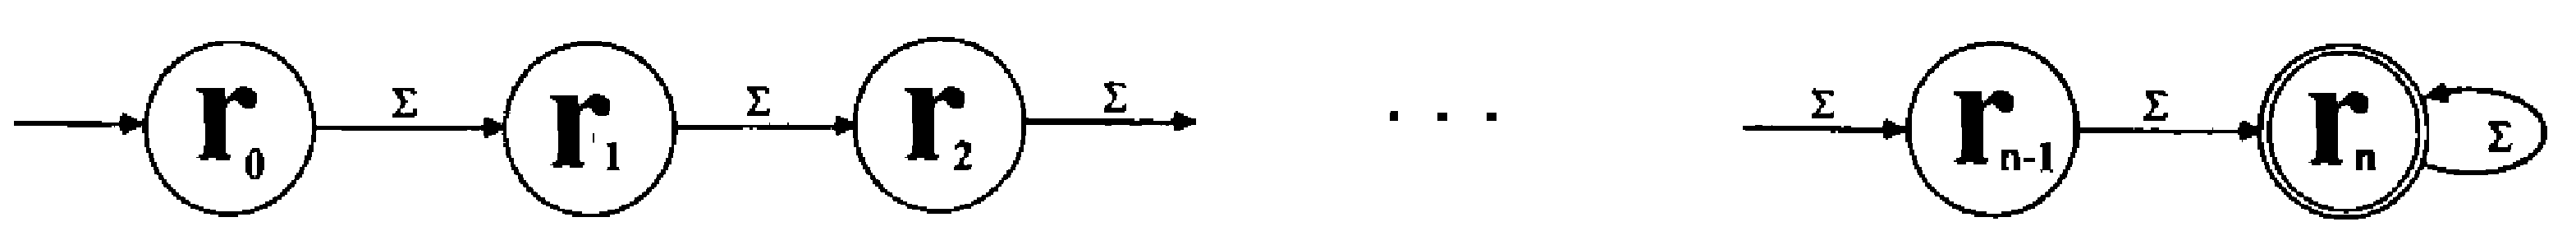
\epsfig{figure=ToFAfigures/fig12-1.eps,width=6in}}
\caption{The automaton $A_n$}\label{fig-12.1}
\end{figure}

The following theorem answers a major question about DFAs: ``Are two
given deterministic finite automata equivalent?'' At first glance,
this appears to be a hard question; an initial strategy might be
to check longer and longer strings, and answer ``No, they are not
equivalent'' if a string is found that is accepted by one machine
but is not accepted by the other. As in the proof of Theorems \ref{thm-12.1}
and \ref{thm-12.2}, we would again be faced with the task of determining when
we could confidently stop checking strings and answer ``Yes, they
are equivalent.''

Such a strategy can be made to work, but an easier method is again
available.  We are essentially checking whether the start state of
the first machine treats strings differently than does the start
state of the second machine. This problem was addressed in Chapter
\ref{ch-3}, and an algorithm that accomplished this sort of checking has
already been presented. This observation provides the basis for the
proof of the following theorem.

% Theorem 12.3
\begin{thm}\label{thm-12.3}
Given any alphabet $\Sigma$ and two DFAs $A_1=\langle\Sigma,S_1,s_{0_1},\delta_1,
F_1\rangle$ and $A_2=\langle\Sigma,S_2,s_{0_2},\delta_2,F_2\rangle$, it is
decidable whether $L(A_1)=L(A_2)$.

\emph{Proof.} Without loss of generality, assume that $S_1\cap S_2=\emptyset$,
and construct a new DFA defined by $A=\langle\Sigma,S_1\cup S_2,s_{0_1},\delta,
F_1\cup F_2\rangle$, where
\begin{center}\begin{tabular}{r@{ = }l}
$(\forall s\in S_1\cup S_2)(\forall\pmb{a}\in\Sigma)\delta(s,\pmb{a})$ &
	$\left\{\begin{tabular}{l@{$\qquad$}l}
		$\delta_1(s,\pmb{a})$, & iff \  $s\in S_1$ \\
		$\delta_2(s,\pmb{a})$, & iff \  $s\in S_2$
		\end{tabular}
	\right.$
\end{tabular}\end{center}
Corollary \ref{cor-3.5} outlines the algorithm for constructing $E_A$ for this machine,
and it should be clear from the definition of $A$ that $s_{0_1}E_As_{0_2}
\Leftrightarrow L(A_1)=L(A_2)$.
\end{thm}

\subsection*{Example 12.2}\label{ex-12.2}

Consider the two machines $A_1$ and $A_2$ displayed in Figure \ref{fig-12.2}. The machine
$A$ constructed according to Theorem \ref{thm-12.3} would look like the diagram inside the
dotted box shown in Figure \ref{fig-12.3}. This new machine is very definitely
disconnected, and in this example $s_{0_1}$ is not related to $s_{0_2}$ by $E_A$ since
these two states treat $\pmb{ab}$ differently ($\pmb{ab}$ is accepted by $A_1$
and rejected by $A_2$). The reader is encouraged to generate another example
using two equivalent machines, and verify that the two original start states
would indeed be related by $E_A$.

% Figure 12.2
\begin{figure}[tbh]
\centerline{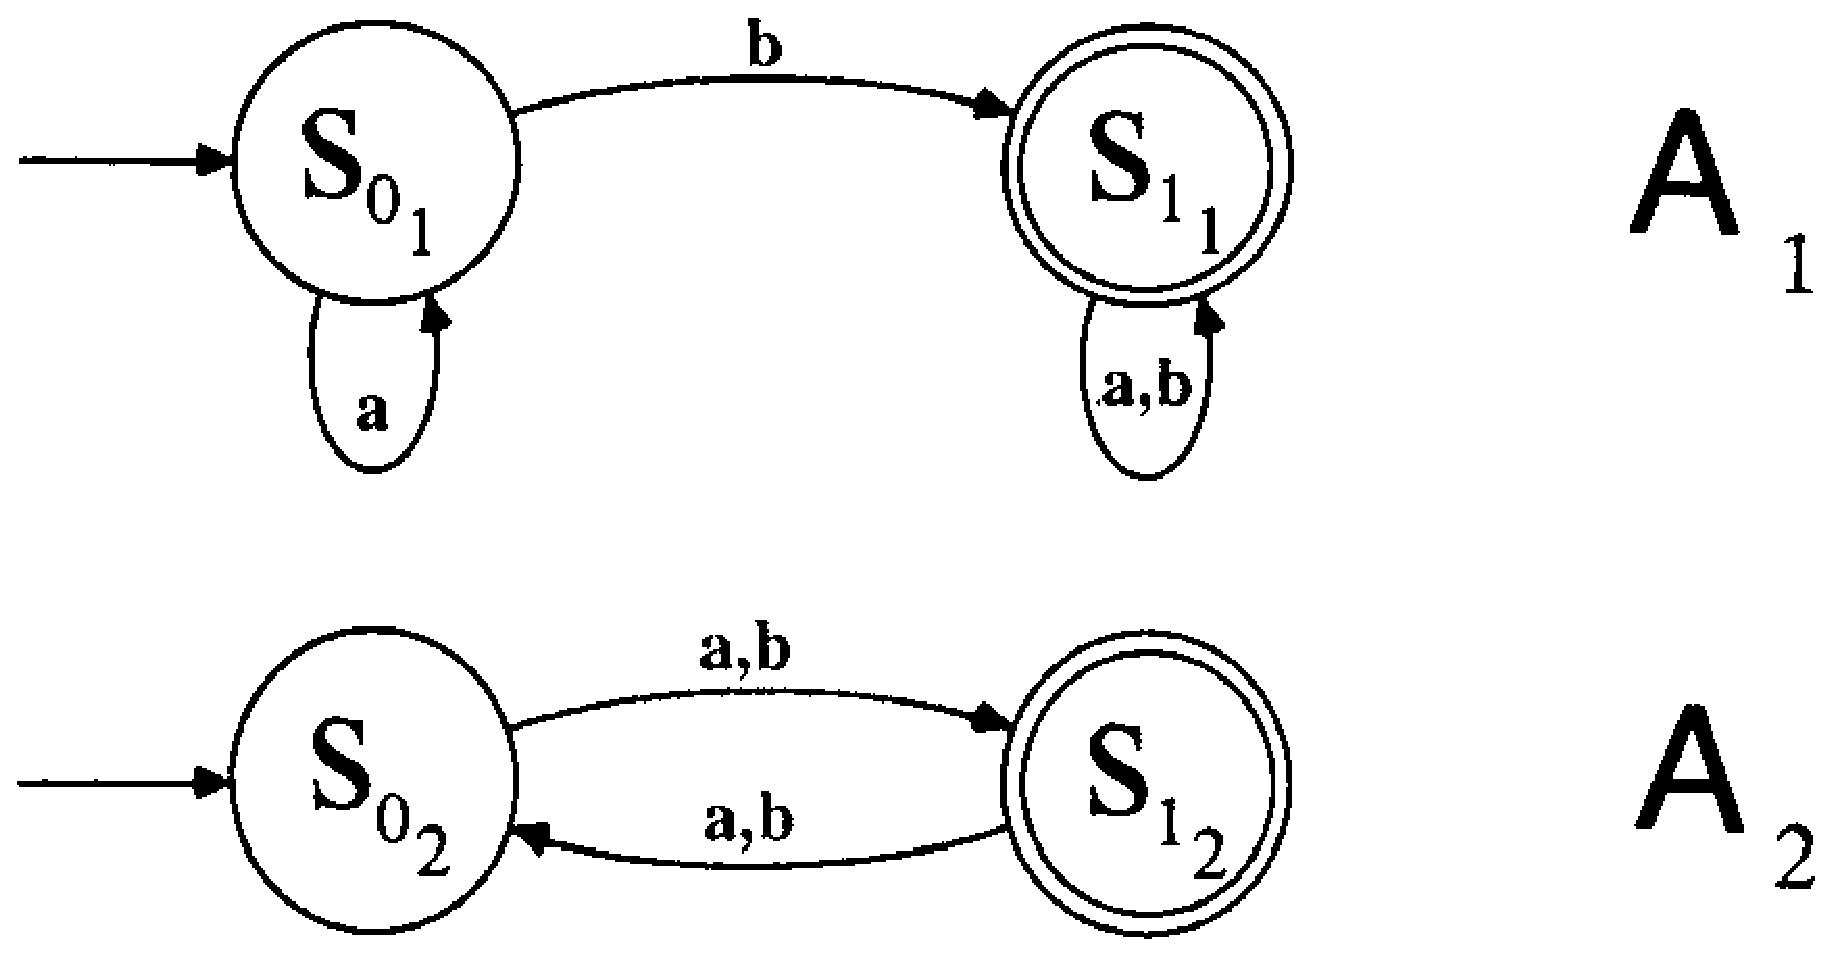
\epsfig{figure=ToFAfigures/fig12-2.eps,width=3.5in}}
%The field \ref{ex-12.2} resolves to '12.1" for some reason...
%\caption{The DFAs discussion in Example \ref{ex-12.2}}\label{fig-12.2}
\caption{The DFAs discussion in Example 12.2}\label{fig-12.2}
\end{figure}

% Figure 12.3
\begin{figure}[tbh]
\centerline{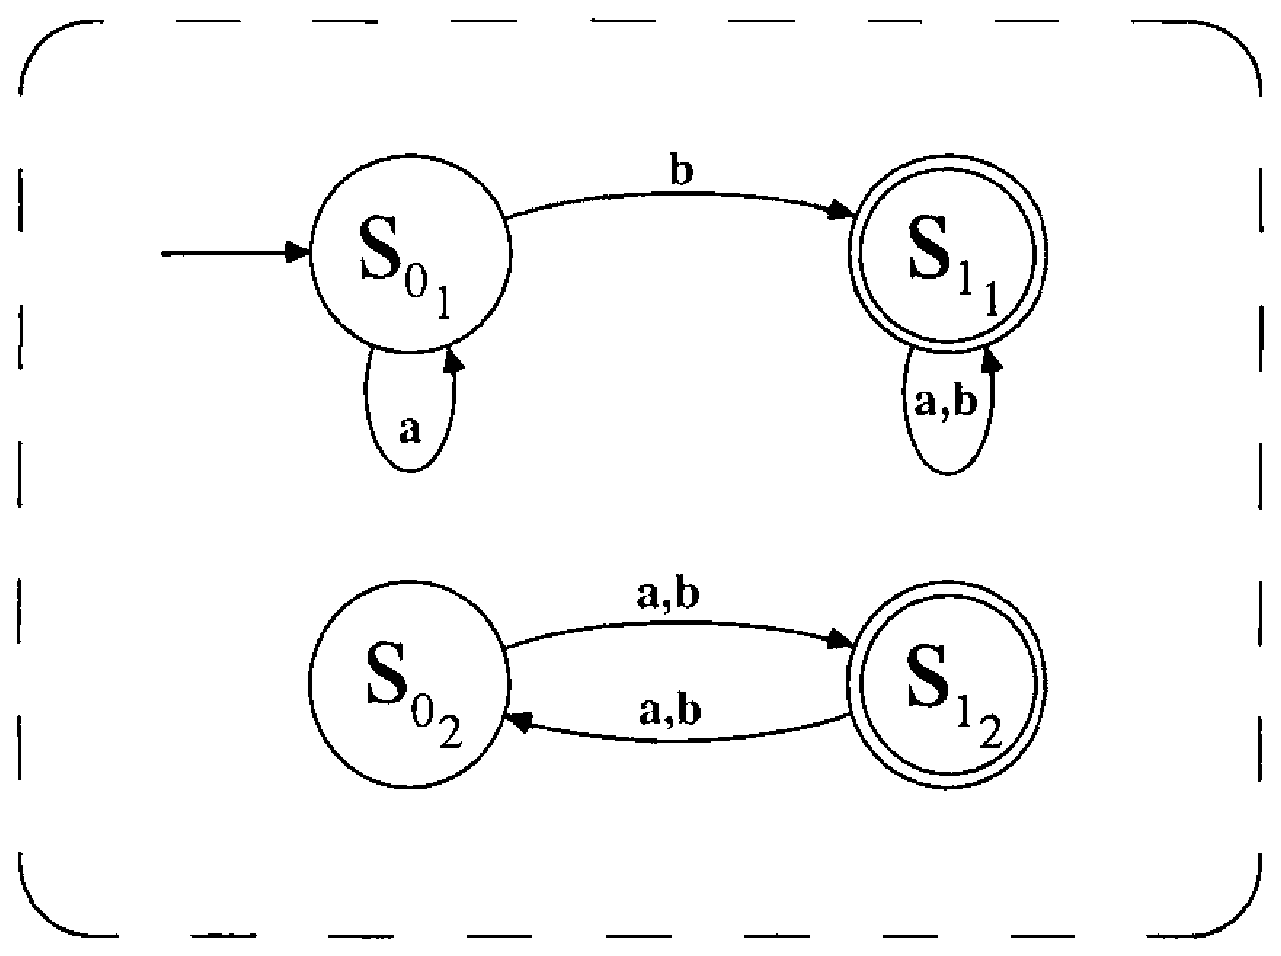
\epsfig{figure=ToFAfigures/fig12-3.eps,width=3.5in}}
%The field \ref{ex-12.2} resolves to '12.1" for some reason...
%\caption{The composite DFA discussed in \ref{ex-12.2}}\label{fig-12.3}
\caption{The composite DFA discussed in Example 12.2}\label{fig-12.3}
\end{figure}

The following theorem explores the relationship between the complexity of a
given regular expression and the size of the corresponding minimal DFA.

% Theorem 12.4
\begin{thm}\label{thm-12.4}
Given any alphabet $\Sigma$ and a regular expression $R$ over $\Sigma$, it is
decidable whether there exists a DFA with fewer than five final states that
accepts the language described by $R$.

\emph{Proof.} Given $R$, Lemma \ref{lmm-6.2} indicates the algorithm (generated
by the constructions presented in Theorems \ref{thm-5.2}, \ref{thm-5.4}, and
\ref{thm-5.5}) for building some NDFA that accepts the regular set corresponding
to $R$. Definition \ref{dfn-4.5} outlines the algorithm for converting this NDFA
into a DFA. Theorem \ref{thm-3.7} and Corollary \ref{cor-3.5} indicate the
algorithms for minimizing this DFA. Counting the number of final states in this
minimal machine will allow the question to be answered correctly.
\end{thm}

The careful reader may have noticed that the minimal machine described in
Chapters \ref{ch-2} and \ref{ch-3} was only advertised to have the minimum
\emph{total} number of states and has not yet been guaranteed to have the smallest
number of \emph{final} states (perhaps there is an equivalent machine with many
more nonfinal states but fewer final states). An investigation of the
relationship between the final states of the minimal machine and the equivalence
classes comprising the right congruence generated by this language will show
that no equivalent DFA can have fewer final states than the minimal machine
has (see the exercises).

The proofs of Theorems \ref{thm-12.3} and \ref{thm-12.4} are good examples of
using existing algorithms to build new algorithms. This technique should be
applied whenever possible in the following exercises. It is certainly useful in
resolving the following question about grammars.

Given two right linear grammars $G_1=\langle\Omega_1,\Sigma,S_1,P_1\rangle$ and
$G_2=\langle\Omega_2,\Sigma,S_2,P_2\rangle$, it is clearly \emph{decidable}
whether $G_2$ is equivalent to $G_1$. An algorithm can be formed that simply:
\begin{enumerate}
\item Uses the construction presented in Lemma \ref{lmm-8.2} to find $A_{G_1}$
	and $A_{G_2}$.
\item Converts these NDFAs to two DFAs called $A_1$ and $A_2$.
\item Appeals to the algorithm presented in Theorem \ref{thm-12.3} to correctly
answer the question.
\end{enumerate}
A trivial extension of this idea proves the following theorem.

% Theorem 12.5
\begin{thm}\label{thm-12.5}
It is decidable whether two given regular grammars $G_1=\langle\Omega_1,\Sigma,
S_1,P_1\rangle$ and $G_2=\langle\Omega_2,\Sigma,S_2,P_2\rangle$ are equivalent.

\emph{Proof.} See the exercises.
\end{thm}

Most of the decidability questions we have asked about languages recognized
by finite automata or described by regular expressions can also be answered
for languages generated by grammars through a similar transformation of existing
algorithms. Such algorithms are generally not the most efficient ones available,
and it can often be instructive to develop a new method from scratch. This is
especially true of the following question, which has no analog in the realms of
finite automata or regular expressions.

% Theorem 12.6
\begin{thm}\label{thm-12.6}
It is decidable whether a given right-linear grammar $G=\langle\Omega,\Sigma,S,
P\rangle$ contains any useless nonterminals.

\emph{Proof.} Recall that a nonterminal is \emph{useless} if it can never appear
in the derivation of any valid terminal string. Essentially, only two things can
prevent a nonterminal $X$ from being effectively used somewhere in a valid
derivation: either $X$ can never appear as part of a partial derivation that
begins with only the start symbol (no matter how many productions we apply), or,
once $X$ is generated, it can never lead to a valid \emph{terminal} string.

Finding the members of $\Omega$ that can be produced from $S$ is a simple
recursive procedure: Begin with $Z_0=\{S\}$ and form $Z_1$ by adding to $Z_0$
all the nonterminals that appear on the right side of productions that are used
to replace $S$. Then form $Z_2$ by adding to $Z_1$ all the nonterminals that
appear on the right side of productions that are used to replace members of $Z_1$
and so on. More formally:
\[ Z_0 = \{S\} \]
and for $i \geq 1$,
\[ Z_{i+1} = Z_i\cup\{Y\in\Omega\ |\ (\exists x\in\Sigma^*)(\exists T\in Z_i)\ni T
	\rightarrow xY\text{ is a production in }P\} \]
Clearly, $Z_0\subseteq Z_1\subseteq\cdots\subseteq Z_n\subseteq\cdots\subseteq
\Omega$, and as was shown for similar collections of nested entities (such as
$E_{0A},E_{1A},\ldots$ in Chapter \ref{ch-3}), after a finite number of steps we
will reach the point where $Z_m=Z_{m+1}$ and $Z_m$ will then represent the set
of \emph{all} nonterminals that can be reached from the start symbol $S$.

In a similar fashion, we can generate another nested sequence of sets $W_0,W_1,
\ldots,$ where $W_i$ represents the set of all nonterminals that can produce
a \emph{terminal} string in $i$ or fewer steps. We are again guaranteed to reach
a point where $W_n=W_{n+i}$ and $W_n$ will indeed be the set of all nonterminals
that can \emph{ever} produce a valid terminal string.

$Z_m\cap W_n$ is thus the set of all \emph{\Index{useful}} members of $\Omega$, and
$\Omega -(Z_m\cap W_n)$ is therefore the set of all \Index{useless} nonterminals.
\end{thm}

\subsection*{Example 12.3}\label{ex-12.3}

$G_4=\langle\{S,A,B,C,V,W,X\},\{\pmb{a},\pmb{b},\pmb{c}\},S,\{S\rightarrow\pmb{a
b}A|\pmb{bb}B|\pmb{cc}V,A\rightarrow\pmb{b}C|\pmb{c}X,B\rightarrow\pmb{ab},
C\rightarrow\lambda|\pmb{c}S,V\rightarrow\pmb{a}V|\pmb{c}X,W\rightarrow\pmb{aa}|
\pmb{a}W,X\rightarrow\pmb{b}V|\pmb{aa}X\}\rangle$ contains three useless
nonterminals, $V$, $W$, and $X$. Recursively calculating the sets described in
the above proof yields:
\begin{center}\begin{tabular}{l@{$\quad$}l}
$Z_0=\{S\}$ & $W_0=\{\ \ \}$ \\
$Z_1=\{S,A,B,V\}$ & $W_1=\{C,B,W\}$ \\ 
$Z_2=\{S,A,B,V,C,X\}$ & $W_2=\{C,B,W,A,S\}$ \\ 
$Z_3=\{S,A,B,V,C,X\}$ & $W_3=\{C,B,W,A,S\}$
\end{tabular}\end{center}
Thus $W$ cannot be generated from the start symbol, and $V$ and $X$ cannot
produce terminal strings. The \emph{useful} symbols are $Z_2\cap W_2=\{S,A,B,C\}$,

The techniques employed here should look somewhat familiar. They involve
iteration methods similar to those developed in Chapter \ref{ch-3}. In fact, it
is possible to apply the connectivity algorithms for nondeterministic finite
automata to this problem by transforming the right-linear grammar $G$ into the
NDFA $A_G$, as defined in the proof of Lemma \ref{lmm-8.2}. The automaton
corresponding to the grammar in Example \ref{ex-12.3} is shown in Figure
\ref{fig-12.4}. Note that the state labeled $\<W\>$ is inaccessible, which
means that it cannot be reached from $\<S\>$. This indicates that there is no
sequence of productions starting with the start symbol $S$ that will produce
a string containing $W$.

Checking whether a nonterminal such as $V$ can produce a terminal string is
tantamount to checking whether the language accepted by $A^V_G$ is nonempty,
where $A^V_G$ is $A_G$ with the start state moved to the state labeled $\<V\>$.
Since both $L(A^V_G)$ and $L(A^X_G)$ are empty, $V$ and $X$ are useless.

\section{Other Decidable Questions}\label{sec-12.2}

It is fairly easy to find succinct algorithms that answer most of the reasonable
questions one might ask about representations of regular languages. For each of
the more complex classes of languages, there are many reasonable questions that
are not decidable. Several of these will be presented in the following sections.
In this section, we consider some of the answerable questions that can be asked
about the more robust machines and grammars.

% Theorem 12.7
\begin{thm}\label{thm-12.7}
Given any context-free grammar $G$, it is decidable whether $L(G)=\emptyset$.

\emph{Proof.} In Theorem 9.3, a scheme was presented that specified how to build
several automata that would be used to identify the useless nonterminals in
$G=\langle\Sigma,\Gamma,S,P\rangle$. Since $L(G)=\emptyset$ iff the start symbol
$S$ is useless, there is an algorithm for testing whether $L(G)=\emptyset$.
\end{thm}

It is also possible to tell whether a context-free grammar generates a finite
or an infinite number of distinct words. The proof is based on the same
principle that was employed in the pumping theorem proof: the presence of long
strings implies that some useful nonterminal $A$ must derive a nontrivial
sentential form containing $A$. The start state $S$ must produce a useful
sentential form containing $A$, and $A$ can then be used to generate an infinite
series of distinct strings.

% Figure 12.4
\begin{figure}
\centerline{\epsfig{figure=ToFAfigures/fig12-4.eps,height=7in}}
\caption{The automaton discussed in Example 12.3}\label{fig-12.4}
\end{figure}

% Theorem 12.8
\begin{thm}\label{thm-12.8}
Given any context-free grammar $G$, it is decidable whether $L(G)$ is infinite.

\emph{Proof.} Let $G=\langle\Sigma,\Gamma,S,P\rangle$ be a context-free grammar.
By Theorem 9.5, there exists a Chomsky normal form grammar $G'=\langle\Sigma,
\Gamma',S,P'\rangle$ that is equivalent to $G$. Let $n=2^{|\Gamma'|}$. By
Theorem \ref{thm-9.7}, any string in $L(G)$ of length $n$ or greater can be
pumped and will imply that $L(G)$ is infinite. An argument similar to that of
Lemma \ref{lmm-12.1} will show that it is sufficient to check strings in the
set $\{y\ |\ y\in\Sigma^*\wedge n\leq |y| < 2n\}$ for membership in $L(G)$. There
are only a finite number of derivation sequences that can produce words in this
range. The algorithm for determining whether $L(G)$ is infinite will check
whether
\[ \{y\ |\ y\in L(G)\wedge n\leq |y| < 2n\} \]
is empty; if so, $L(G)$ is finite, and $L(G)$ is infinite otherwise.
\end{thm}

The exercises explore more efficient methods for searching for a string that
can be pumped. The intimate correspondence between context-free grammars and
pushdown automata guarantees that similar questions about PDAs are decidable.

% Corollary 12.1
\begin{cor}\label{cor-12.1}
Given any pushdown automaton $P$, it is decidable whether:
\begin{enumerate}[{\bf a.}]
\item $L(P)$ is empty.
\item $L(P)$ is finite.
\item $L(P)$ is infinite.
\end{enumerate}

\emph{Proof.} By Theorem \ref{thm-10.3}, every PDA $P$ has a corresponding
context-free grammar $G_P$. The algorithms described in Theorems \ref{thm-12.7}
and \ref{thm-12.8} can be applied to $G_P$ to determine the nature of $L(G_P)$,
and since $L(P)=L(G_P)$, the same questions about $P$ are likewise decidable.
\end{cor}

Given a particular word $x$ and a context-free grammar $G$, it is decidable
whether $x$ can be generated by $G$. In fact, this question can be decided for
context-sensitive grammars, too. The proof heavily relies on the fact that no
sentential form longer than $x$ can possibly generate $x$ in the absence of
contracting productions in the grammar.

% Theorem 12.9
\begin{thm}\label{thm-12.9}
Given any context-sensitive grammar $G$ and any word $x$, it is decidable
whether $x\in L(G)$.

\emph{Proof.} Let $G=\langle\Sigma,\Gamma,S,P\rangle$ be a context-sensitive
grammar and let $x\in\Sigma^n$ (for an arbitrary $n$). It is possible to construct a (finite) graph and
apply existing algorithms from graph theory to answer the question of whether
$G$ generates $x$. The nodes of the graph will correspond to the strings from
$(\Sigma\cup\Gamma)^*$ of length $n$ or less. The (directed) edges from a node
representing a given sentential form $w$ lead to the strings (of length $n$ or
less) that can be generated from $w$ by applying a single production from $P$.
Both the sentential form $x$ and $S$ will appear in this graph, and the question
of whether $x\in L(G)$ is equivalent to the question of whether there is a path
from $S$ to $x$. There are many standard algorithms for determining paths and
components in a graph, and thus the question of whether $x\in L(G)$ is decidable.
\end{thm}

The generation of all the edges in the graph generally involves more effort
than is needed to answer the question. A more efficient method is similar to
the recursive calculations used to find the set of connected states in a DFA.
Beginning with $\{S\}$, the production set $P$ can be consulted to determine the
labels of nodes that can be derived from $S$ in one step. These new labels can
be added to the set of accessible sentential forms, and the added nodes can be
checked until no new labels are found. The set of sentential forms will then 
consist of
\[ \{w\in(\Sigma\cup\Gamma)^*|\ S\ \DRightarrow w \wedge |w|\leq n\} \]
and contain all words in $L(G)$ of length $\leq n$, If we are only interested in
the specific word $x$, then the algorithm can return Yes as soon as $x$ appears
in the set of accessible sentential forms and would return No if $x$ did not
appear by the time the set stopped growing.

The above algorithm will suffice for any grammar that does not contain
contracting productions, but can clearly give the wrong answers when applied to
type 0 grammars. Since the length of sentential forms can both grow and shrink
in unrestricted grammars, the word $x$ may actually be generated by a sequence
of productions that at some point generates a sentential form longer than $x$.
Such a sequence would not be considered by the method outlined in Theorem
\ref{thm-12.9}, and the algorithm might answer No when the correct answer is Yes.
We could define a procedure that looked at larger and larger graphs (consisting
of more and longer sentential forms), which would halt and answer Yes if a
derivation sequence for $x$ was discovered. If $x$ actually can be generated by
$G$, this method will eventually uncover the appropriate sequence. We therefore
have a procedure that will reliably tell us if a word can be generated by an
unrestricted grammar. Unless we include a specification of when to stop and
answer No, this procedure is not an algorithm. In later sections, we will see
that it is \emph{impossible} to determine, for an arbitrary type 0 grammar $G$,
if an arbitrary word $x$ is not generated by $G$. The question of whether $x\in
L(G)$ is not decidable for arbitrary grammars.

It turns out that there are many reasonable questions such as this one that
cannot be determined algorithmically. We begin our overview of undecidable
problems with an analysis of a very reasonable question concerning Pascal
programs. Subsequent sections consider undecidable questions concerning the
grammars and machines covered in this text.

\section{An Undecidable Problem}\label{sec-12.3}\index{undecidable problems}

Having now developed a false sense of security about our ability to produce
algorithms for determining many properties about machines and languages, we
now step back and see whether there is anything we cannot do algorithmically. A
simple counting argument will show that there are too many things to calculate
and not enough algorithms with which to calculate them all. It may be helpful to
review the section on cardinality in Chapter \ref{ch-0} and recall that there
are different orders of infinity. A diagonalization argument showed that the
natural numbers could not be put in one-to-one correspondence with the real
numbers; there are simply too many real numbers to allow such a matching to
occur. A similar mismatch occurs when comparing the (countable) number of
algorithms to the (uncountable) number of possible yes-no functions.

By definition, an algorithm is a \emph{finite} list of instructions, written
over some finite character set. As such, there are only a countable number of
different algorithms that can be written. It may be helpful to consider the set
of all Pascal programs and view each file that contains the ASCII code for a
program, which is essentially a sequence of zeros and ones, as one very long
binary integer. Clearly, an infinite number of Pascal programs can be written,
but no more programs than there are binary integers, so the number of such files
is indeed countable.

Now consider the possible lists of answers that could be given to questions
involving a countable number of instances. We will argue that there are an
uncountable number of yes-no patterns that might describe the answers to such
questions. Notice that the descriptions for automata, grammars, and the like
are also finite, and thus there are a countable number of DFAs, a countable
number of grammars, and so on, that can be described. The questions we asked in
the previous sections were therefore applied to a countable number of instances,
and these instances could be ordered in some well-defined way, much as the
natural numbers are ordered. If we think of a yes response corresponding to the
digit 1 and a no response corresponding to 0, then the corresponding series of
answers to a particular question can be thought of as an unending sequence of
0s and 1s. By placing a decimal point at the beginning of the sequence, each
such pattern can be thought of as a binary fraction, representing a real number
between $.00000\ldots=0$ and $.111111\ldots=1$. Conversely, each such real
number in this range represents a sequence of yes-no answers to some question.
Since there are an uncountable number of real numbers between 0 and 1, there are
an uncountable number of answers that might be of interest to us. Some of these
answers cannot be obtained by algorithms, since there are not enough algorithms
to go around. Thus, there must be many questions that are not decidable.

It is not immediately apparent that the existence of undecidable questions is
much of a drawback; perhaps all the ``interesting'' questions are decidable.
After all, there are an uncountable number of real numbers, yet all computers
and many humans seem to make do with just the countable number of rational
numbers. Unfortunately, there are many simple and meaningful questions that are
undecidable. We discuss one such question now; others are considered in the next
section.

Just about every programmer has had the experience of running a program that
never produces any output and never shows any sign of halting. For programs
that are fairly short, this is usually not a problem. For major projects that
are expected to take a very long time, there comes an agonizing moment when we
have to give up hope that it is on the verge of producing a useful answer and
stop the program on the assumption that it has entered an infinite loop. While
it would be very nice to have a utility that would look over a program and
predict how long it would run, most of us would settle for a device that would
simply predict whether or not it will ever halt.

It's a good bet that you have never used such a device, which may at first seem
strange since a solution to the \emph\Index{halting problem} would certainly provide
information that would often be useful. If you have never thought about this
before, you might surmise that the scarcity of such programs is a consequence of
any one of several limiting factors. Perhaps they are inordinately expensive to
run, or no one has taken the time to implement an existing scheme, or perhaps no
one has yet figured out how to develop the appropriate algorithms. In actuality,
no one is even looking for a ``halting'' algorithm, since no such algorithm can
possibly exist.

\index{undecidable problems!Pascal halting problem|(}Let us consider the implications that would arise if such an algorithm could be
programmed in, say, Pascal. We can consider such an algorithm to be implemented
as a Boolean function called HALT, which looks at whatever program happens to
be in the file named data.p and returns the value TRUE if that program will
halt, and returns FALSE if the program in data.p would never halt. Perhaps this
function is general enough to look at source code for many different languages,
but we will see that it is impossible for it to simply respond correctly even
when looking solely at Pascal programs.

The programmer of the function HALT would likely have envisioned it to be used
in a program such as CHECK, shown in Figure \ref{fig-12.5}. We will use it in a
slightly different way and show that a contradiction arises if HALT really did
solve the halting problem. Our specific assumptions are that:
\begin{enumerate}
\item HALT is written in Pascal.
\item HALT always gives a correct answer to the halting problem, which means:
\begin{enumerate}
\item It always returns an answer after a finite amount of time.
\item The answer returned is FALSE if the Pascal program in data.p would never
halt.
\item The answer returned is TRUE if the Pascal program in data.p would halt (or
if the program in data.p will not compile).
\end{enumerate}
\end{enumerate}

Consider the program TEST in Figure \ref{fig-12.6}, which is structured so that
it will run forever if the function HALT indicates that the program in the file
data.p would halt, and simply quits if HALT indicates that the program in data.p
would not halt. Some interesting things happen if we run this program after
putting a copy of the source code for TEST in data.p.

If HALT does not produce an answer, then HALT certainly does not behave as
advertised, and we have an immediate contradiction. HALT is supposed to be an
algorithm, so it must eventually return with an answer. Since HALT is a Boolean
function, we have only two other cases to consider.

% Figure 12.5
\begin{figure}
{\tt
\begin{tabbing}
abc\=abc\=end \kill
program CHECK; \\
\{ envisioned usage of HALT \} \\
\> function HALT:boolean; \\
\> begin \\
\>\> \{ marvelous code goes here \} \\
\> end \{ HALT \} \\
\\
begin \{ CHECK \} \\
if HALT then \\
\> writeln('The program in file data.p will halt') \\
else \\
\> writeln('The program in file data.p will not halt') \\
end \{ CHECK \}.
\end{tabbing}
}
\caption{A possible usage of HALT}\label{fig-12.5}
\end{figure}

{\bf Case 1}: HALT returns a value of TRUE to the calling program TEST. This has
two consequences, the first of which is implied by the asserted behavior of HALT.
\begin{enumerate}[i.]
\item If halt does what it is supposed to do, this means that the program in
data.p halts. We ran this program with the source code for TEST in data.p, so
TEST must actually halt.
\end{enumerate}
The second consequence comes from examining the code for TEST, and noting
what happens when HALT returns TRUE.
\begin{enumerate}[i.]
\addtocounter{enumi}{1}
\item The {\tt if} statement in the program TEST then causes the infinite loop
to be entered, and TEST runs forever, doing nothing particularly useful.
\end{enumerate}
Our two consequences are that TEST halts and TEST does not halt. This is a
clear contradiction, and so case 1 never occurs.

{\bf Case 2}: HALT returns a value of FALSE to the calling program TEST. This
likewise has two consequences. Considering the advertised behavior of HALT, this
must mean that the program in data.p, TEST, must not halt. However, the code for
TEST shows that if HALT returns FALSE we execute the else statement, write one
line, and then stop. TEST therefore halts. TEST must again both halt and not
halt.

Whichever way we turn, we reach a contradiction. The only possible conclusion
is that the function HALT does not behave as advertised. It must either return
no answer, or give an incorrect answer.

It should be clear that the problem cannot be fixed by having the programmer who
proposed the function HALT fiddle with the code; the above contradiction will be
reached regardless of what code appears between the {\tt begin} and {\tt end}
statements in the function HALT. We have shown that any such proposed function
is guaranteed to behave inappropriately when fed a program such as TEST. In
actuality, there are an infinite number of programs that cause HALT to misbehave,
but it was sufficient to demonstrate just one failure to justify that no such
function can solve the general problem.

% Figure 12.6
\begin{figure}
{\tt
\begin{tabbing}
abc\=abc\=end\kill
program TEST; \\
\{ to be placed in the file data.p \} \\
var FOREVER: boolean; \\
\> function HALT: boolean; \\
\> begin \\
\>\> \{ marvelous code goes here \} \\
\> end; \{ HALT \} \\
\\
begin \{ TEST \} \\
FOREVER := false; \\
if HALT then \\
\> repeat \\
\>\> FOREVER := false; \\
\> until FOREVER \\
else \\
\> writeln('This program halts') \\
end \{ TEST \}.
\end{tabbing}
}.
\caption{Another program incorporating HALT}\label{fig-12.6}
\end{figure}

\index{halting problem!in Pascal}
The above argument demonstrates that the \emph{halting problem} for
Pascal programs is \emph{\Index{undecidable}} or \emph{\Index{unsolvable}}. That
is, there does not exist a Pascal program that can always decide correctly, when
fed an arbitrary Pascal program, whether that program halts.

If we were to define an algorithm as ``something that can be programmed in
Pascal,'' we would have shown that there is no algorithm for deciding whether
an arbitrary Pascal program halts. One might suspect that this is therefore not
a very satisfying definition of what an algorithm is, since we have a concise,
well-stated problem that cannot be solved using Pascal. It is generally agreed
that the problem does not lie with some overlooked feature that was
inadvertently not incorporated into Pascal. Clearly, all programming languages
suffer from similar inadequacies. For example, an argument similar to the one
presented for Pascal would show that no C program can be devised that can tell
which C programs can halt. Thus, no other programming language can provide a
more robust definition of what an algorithm is.

\index{halting problem!in C}\index{undecidable problems!C halting problem}
There are variations on this theme that likewise lead to contradictions. Might
there be a Pascal program that can check which C programs can halt? If you
believe that every Pascal program can be rewritten as an equivalent C program,
the answer is definitely no; a Pascal program that checks C programs could then
be rewritten as a C program (which checks C programs), and we again reach a
contradiction.\index{undecidable problems!Pascal halting problem|)}

It is generally agreed that the limitations do not arise from some correctable
inadequacy in our current methods of implementing algorithms. That is, the
limitations of algorithmic solutions seem to be inherent in the nature of
algorithms. Programming languages, Turing machines, grammars, and all other
proposed systems for implementing algorithms have been shown to be subject to
the same limitations in computational power. The use of Turing machines to
implement algorithms has several implications that apply to the theory of
languages. These are explored in the following sections.

\section{Turing Decidability}\label{sec-12.4}\index{Turing machine!undecidable problems}

In the previous section, we saw that no Pascal program could always correctly
predict when another Pascal program would halt. A similar statement was true
for C programs, and Turing machines, considered as computing devices, are no
different; no Turing machine solves the halting problem.

Each of us is probably familiar with the way in which a Pascal program reads a
file, and hence it is not hard to imagine a Pascal program that reacts to the
code for another Pascal program. As long as the input alphabet contains at least
two symbols, encodings can be defined for the structure of a Turing machine,
which allows the blueprint for its finite state control to be placed on the
input tape of another Turing machine. A binary encoding\index{Turing machine!encoding} might be given for the
number of states, followed by codes that enumerate the moves from each of the
states. Just as we are not presently concerned about the exact ASCII codes that
define the individual characters in a file containing a Pascal program, we need
not be concerned with the specific representation used to encode a Turing
machine on an input tape.

Consider input tapes that contain the encoding of a Turing machine, followed
by some delimiter, followed by an input word. Assume there exists a Turing
machine $H$ that, given such an encoding of an arbitrary machine and an input word,
always correctly predicts whether the Turing machine represented by that
encoding halts for that particular word. This assumption leads to a
contradiction exactly as shown in the last section for Pascal programs. We would
be able to use the machine $H$ as a submachine in another Turing machine that
halts exactly when it is not supposed to halt, and thereby show that $H$ cannot
possibly behave properly.

% Theorem 12.10
\begin{thm}\label{thm-12.10}\index{undecidable problems!Turing machine halting problems|(}
Given a Turing machine $M$ and a word $w$, it is undecidable whether $M$ halts
when the string $w$ is placed on the input tape.

\emph{Proof.} The proof is essentially the same argument that was presented in
the last section.
\end{thm}

We will see that the unsolvability of the halting problem will imply that it
is not decidable whether a given string will cause a Turing machine to halt and
print $\pmb{Y}$. If a word is accepted, this fact can eventually be discovered,
but we cannot reliably tell which words are rejected by an arbitrary Turing
machine. If we could, we would have an algorithm for computing the complement of
any Turing-acceptable language. In the next section, we will show that there are
Turing-acceptable languages that have complements that are not Turing-acceptable,
which means that a general algorithm for computing complements cannot exist.

A problem equivalent to the halting problem involves the question of whether
an arbitrary type 0 grammar accepts a given word. This can be seen to be almost
the same question as was asked of Turing machines.

% Theorem 12.11
\begin{thm}\label{thm-12.11}
Given a type 0 grammar $G$ and a word $w$, it is undecidable whether $G$
generates $w$.

\emph{Proof.} If this question were decidable, it would provide an algorithm for
solving the halting problem, which is known to be undecidable. That is, if there
existed an algorithm for deciding whether $w\in L(G)$, there would also be an
algorithm for deciding whether $w$ is accepted by a Turing machine. The Turing
machine algorithm would operate as follows:

Given an arbitrary Turing machine $M$, modify $M$ to produce $M'$, an equivalent
machine that halts only when it accepts. Use Definition 11.8 to find the
corresponding type 0 grammar $G_{M'}$, which is also equivalent to $M$. The
algorithm that predicts whether $w\in L(G_{M'})$ can now be used to decide
whether $M$ halts on input $w$.

This scheme would therefore solve the halting problem for an arbitrary Turing
machine, and hence the algorithm that predicts whether $w\in L(G)$ cannot exist.
Thus, $w\in L(G)$ is undecidable for arbitrary type 0 grammars.
\end{thm}

Given the intimate correspondence between Turing machines and type 0 grammars,
it is perhaps not surprising that it is just as hard to solve the membership
question for type 0 grammars as it was to solve the halting problem for Turing
machines. We now consider a question that may initially appear to be more
tractable than the halting problem. However, it will be shown to be unsolvable
by the same reasoning used in the last theorem: if this question could be
decided, then the halting problem would be decidable.

% Theorem 12.12
\begin{thm}\label{thm-12.12}
Given an arbitrary Turing machine $T$, it is undecidable whether $T$ accepts
$\lambda$.

\emph{Proof.} Assume that there exists an algorithm for deciding whether $T$
accepts $\lambda$. That is, assume that there exists a Turing machine $X$ that,
when fed an encoding of any Turing machine $T$, halts with $\pmb{Y}$ when $T$
would accept $\lambda$ and halts with $\pmb{N}$ whenever $T$ rejects $\lambda$.
$X$ can then be used to determine whether an arbitrary Turing machine $M$ would
accept an arbitrary word $x$. Given a machine $M$ and a string $x$, it is easy
to modify $M$ to produce a new Turing machine $T_{M_x}$, which accepts $\lambda$
exactly when $M$ accepts $x$. $T_{M_x}$, is formed by adding a new start state
that checks whether the read head is initially scanning a blank (that is, if
$\lambda$ is on the input tape). If not, control remains in this state, and
$T_{M_x}$ never halts. However, if the initially scanned symbol is a blank, new
states are used to write $x$ on the input tape and return the read head to the
leftmost symbol of $x$. Control then passes to the original start state of $M$.
In this manner, $T_{M_x}$ accepts $\lambda$ exactly when $M$ accepts $x$.

This correspondence makes it possible to use the Turing machine $X$ as a
submachine in another Turing machine $X_H$ that solves the halting problem. That
is, given an input tape with an encoding of a machine $M$ followed by the
symbols for a word $x$, $X_H$ can be easily programmed to modify the encoding of
$M$ to produce the encoding of $T_{M_x}$ and leave this new encoding on the
input tape before passing control to the submachine $X$. $X_H $then accepts
exactly when $T_{M_x}$ accepts $\lambda$, which happens exactly when the original machine $M$ halts
on input $x$. $X_H$ would therefore represent an algorithm for solving the
halting problem, which we know cannot exist. The portion of the machine that
modifies the encoding of $M$ is quite elementary, so it must be the submachine
$X$ that cannot exist. Thus, there is no algorithm that can accomplish the task
for which $X$ was designed, that is, determining whether an arbitrary Turing
machine $T$ accepts the empty string.
\end{thm}

The conclusion that $X$ was the portion of $X_H$ that behaves improperly is akin
to the observation in the previous section that the main part of the Pascal
program TEST was valid, and hence it must be the function HALT that behaves
incorrectly.\index{undecidable problems!Turing machine halting problems|)}

\section{Turing-Decidable Languages}\label{sec-12.5}

We now consider languages whose criteria for membership is related to the
halting problem. Define the language $D$ to be those words that either are not
encodings of Turing machines or are encodings of machines that would halt with
$\pmb{Y}$ when presented with their own encoding on their input tape. The
language $D$ is Turing acceptable, since a multitape machine\index{multi-tape Turing machine}\index{Turing machine!multi-tape} could copy the
input word to a second tape, check whether the encoding truly represented a
valid Turing machine, and then use the ``directions'' on the second tape to
simulate the action of the encoded machine on the original input. The multitape
machine would halt with $\pmb{Y}$ if the encoding was invalid or if the
simulated machine ever accepts.

On the other hand, the complement of $D$ is not Turing acceptable. Let $U$ be
the set of all valid encodings of Turing machines that do \emph{not} halt when
fed their own encodings. Then $U=\ \sim\!\!D$, and there does not exist a
machine $T$ for which $L(T)=U$. If such a machine existed, it would have an
encoding, and this leads to the same problem encountered with the HALT function
in Pascal. This encoding of $T$ is either a word in $U$ or is not a word in $U$;
both cases lead to contradictions. If the encoding of $T$ belongs to $U$, then
by definition of $U$ it does not halt when fed its own encoding. But the
assumption that $L(T)=U$ requires that $T$ halt with $\pmb{Y}$ for all encodings
belonging to $U$, which means $T$ must halt when fed its own encoding. A similar
contradiction is also reached if the encoding of $T$ does not belong to $U$.
Therefore, no such Turing machine $T$ can exist, and $U$ is an example of a
language that is not Turing-acceptable.

We have finally found a language that is not type 0. A counting argument would
have shown that, since there are only a countable number of type 0 grammars and
an uncountable number of subsets of $\Sigma^*$, there had to be many languages
over $\Sigma$ that are not in \ZSIG\ ( $=\TSIG$). We have now seen that some of these
unrepresentable languages are meaningful sets for which it would be quite
desirable to be able to recognize or generate.

% Theorem 12.13
\begin{thm}\label{thm-12.13}
If $\|\Sigma\|\geq 2$, then \TSIG\ is not closed under complementation.

\emph{Proof.} Encodings of arbitrary Turing machines can be effectively
accomplished with only two distinct symbols in the alphabet. The
Turing-acceptable language $D$ described above has a complement $U$ that is not
Turing-acceptable.
\end{thm}

Our original criteria for belonging to the language $L$ accepted by a Turing
machine $M$ implied that $M$ would eventually halt when presented with any word
in $L$, but we had no guarantees about how $M$ will behave when presented with a
word that is not in $L$. $M$ may halt with $\pmb{N}$ on the tape, or $M$ may run
forever. Indeed, we have just seen a Turing-acceptable language for which this
will be the best we can hope for. Turing machines therefore embody
\emph{procedures}, which are essentially a deterministic set of step-by-step
instructions. We now consider the languages accepted by the subclass of Turing
machines that correspond to \emph{algorithms}, procedures that are guaranteed to
eventually halt under all circumstances.

% Definition 12.2
\begin{dfn}\label{dfn-12.2}\index{H@\HSIG \ (H-sigma )}
Let $\Sigma$ be an alphabet. Define \HSIG\ to be the collection of all
languages that can be recognized by Turing machines that halt on all input.
\end{dfn}

Languages in \HSIG\ are called \emph{\Index{Turing-decidable languages}}\index{language!Turing-decidable}. A
trivial modification shows that $L\in\HSIG$ if there exists a Turing machine
that not only halts upon placing a $\pmb{Y}$ after the input word on an
otherwise blank tape for accepted words, but similarly preserves the input word
and prints $\pmb{N}$ for each rejected string. Such devices will be referred to
as \emph{halting} Turing machines.

% Theorem 12.14
\begin{thm}\label{thm-12.14}
\HSIG\ is closed under complementation.

\emph{Proof.} Let $L$ be a Turing-decidable language. Then there must exist a
Turing machine $H$ for which $L(H)=L$ and that halts with $\pmb{Y}$ or $\pmb{N}$
for all strings in $\Sigma^*$. The finite-state control of $H$ can be easily
modified to produce a Turing machine $H'$ for which $L(H')=\ \sim\!\!L$. All
that is required is to replace every transition in $H$ that prints $\pmb{N}$
with a similar transition that prints $\pmb{Y}$ and likewise make sure that
$\pmb{N}$ will be printed by $H'$ whenever $H$ prints $\pmb{Y}$.
\end{thm}

This result has some immediate consequences.

% Corollary 12.2
\begin{cor}\label{cor-12.2}
There is a language that is Turing acceptable but not Turing decidable. That is,
$\HSIG\subset\TSIG$

\emph{Proof.} Definition \ref{dfn-12.2} implies that $\HSIG\subseteq\TSIG$. By
Theorems \ref{thm-12.13} and \ref{thm-12.14}, these two classes have different
closure properties, and thus they cannot be equal. Therefore, $\HSIG\subset
\TSIG$.
\end{cor}

Actually, we have already seen a language that is Turing acceptable but not
Turing decidable. $D$ was shown to be Turing acceptable, but if $D$ were Turing
decidable, then its complement would be Turing decidable by Theorem
\ref{thm-12.14}. However, $\sim\!\!D=U$, and $U$ is definitely not Turing
decidable since it is not even Turing acceptable.

\OSIG, the context-sensitive languages, is another subclass of \TSIG. It is
possible to determine how \HSIG\ relates to \OSIG\ and thereby insert \HSIG\
into the language hierarchy.

% Corollary 12.3
\begin{cor}\label{cor-12.3}
Every context-sensitive language is Turing decidable. That is, $\OSIG\subseteq
\HSIG$

\emph{Proof.} This is actually a corollary of Theorem \ref{thm-12.9}. Given a
type 1 language $L$, there is a context-sensitive grammar $G$ that generates $L$.
The proof of Theorem \ref{thm-12.9} presented an algorithm for determining
whether an arbitrary word can be generated by $G$. This algorithm can be
implemented as a Turing machine $T_G$ that can determine whether a given word
can be generated by $G$ and always halts with the correct answer. Thus, $L$ is
Turing decidable.
\end{cor}

These implications provide the missing element in the proof of Theorem 11.10, as
stated in the next corollary.

% Corollary 12.4
\begin{cor}\label{cor-12.4}
The class of context-sensitive languages is properly contained in the class of
Turing acceptable languages. That is, $\OSIG\subset\TSIG$.

\emph{Proof.} By the previous corollaries, $\OSIG\subseteq\HSIG$ and $\HSIG
\subset\TSIG$.
\end{cor}

Actually, the context-sensitive languages are properly contained in \HSIG. This
will be shown by exhibiting a language that is recognized by a Turing machine
that halts on all inputs, but that cannot be generated by any context-sensitive
language. The following proof, based on diagonalization, should by now look
familiar.

% Theorem 12.15
\begin{thm}\label{thm-12.15}
Let $\Sigma$ be an alphabet for which $\|\Sigma\|\geq 2$. There is a language
that is Turing decidable but not context sensitive. That is, $\OSIG\subset\HSIG$.

\emph{Proof.} By Corollary \ref{cor-12.3}, $\OSIG\subseteq\HSIG$, and it remains
to be shown that there is a member of \HSIG\ that is not a member of \OSIG. By
the technique described in Theorem \ref{thm-12.9}, every context-sensitive
grammar can be represented by a halting Turing machine, and each such Turing
machine has an encoding of its finite-state control. Define $L$ to be the set of
all encodings of Turing machines that:
\begin{enumerate}
\item Represent context-sensitive grammars.
\item Reject their own encoding.
\end{enumerate}
Providing a scheme for encoding the quadruple for a context-sensitive grammar
is left for the exercises. Any reasonable encoding scheme will make it a simple
task to determine whether a candidate string represents nonsense or a valid
context-sensitive grammar.

$L$ can therefore be recognized by a halting Turing machine that:
\begin{enumerate}
\item Checks if the string on the input tape represents the encoding of a valid
context-sensitive grammar.
\item Calculates the encoding of the corresponding Turing machine.
\item Simulates that Turing machine being fed its own encoding.
\end{enumerate}
This process is guaranteed to halt, since the Turing machine being simulated is
known to be a halting Turing machine. Thus, $L\in\HSIG$. However, if $L\in\OSIG$,
we find ourselves in a familiar dilemma. If there is a context-sensitive grammar
$G_L$ that generates $L$, then this grammar would have a corresponding Turing
machine $T_L$, which would have an encoding $x_L$. If $x_L$ did not belong to
$L$, then by definition of $L$ it would be an encoding of a machine ($T_L$) that
did not reject its own encoding ($x_L$). Thus, $T_L$ recognizes $x_L$, and
therefore the corresponding grammar $G_L$ must generate $X_L$. But then $X_L\in
L(G_L)=L$, contradicting the assumption that $X_L$ did not belong to $L$. If on
the other hand $X_L$ belongs to $L$, then, by definition of $L$, $T_L$ must
reject its own encoding ($x_L$), and thus $x_L\notin L(T_L)=L(G_L)=L$, which is
another contradiction. Thus, no such context-sensitive grammar $G_L$ can exist,
and $L$ is not a context-sensitive language.
\end{thm}

The above diagonalization technique can be generalized; given any enumerable
class $\mathfrak{M}$ of languages whose members are all represented by halting
Turing machines, there must exist a halting Turing machine that recognizes a
language not in $\mathfrak{M}$ (see the exercises). The following theorem
summarizes how the other classes of languages discussed in the text fit in the
language hierarchy.

% Theorem 12.16
\begin{thm}\label{thm-12.16}\index{hierarchy!of language classes}.
Let $\Sigma$ be an alphabet for which $\|\Sigma\|\geq 2$. Then
\[ \DSIG=\WSIG=\RSIG=\GSIG\subset\ASIG\subset\CSIG=\PSIG\subset\LSIG=\OSIG
	\subset\HSIG\subset\ZSIG=\TSIG\subset\wp(\Sigma^*) \]

\emph{Proof.} The relationship between the type 0, type 1, type 2, and type 3
languages was outlined in Theorem \ref{thm-11.10}. Theorem \ref{thm-10.8} showed
that \ASIG\ properly lies between the type 3 and type 2 languages. Corollary
\ref{cor-12.2} and Theorem \ref{thm-12.15} show that \HSIG properly lies between
the type 1 and type 0 languages and also show that the type 1 languages are a
proper subset of the type 0 languages. The existence of languages that are not
Turing acceptable shows that \TSIG\ is properly contained in $\wp(\Sigma^*)$. A
counting argument shows that proper containment of \TSIG\ in $\wp(\Sigma^*)$
also holds even if\ \ $\Sigma$ is a singleton set.
\end{thm}

The relationships between six distinct and nontrivial classes of languages are
characterized by Theorem 12.16. Each of these classes is defined by a particular
type of automaton. The trivial class of all languages, $\wp(\Sigma^*)$, was
shown to have no mechanical counterpart. We have seen that type 3 languages
appear in many useful applications. Program design, lexical analysis, and
various engineering problems are aided by the use of finite automata concepts.
Programming languages are always defined in such a way that they belong to the
class \ASIG, since compilers should operate deterministically. The theory of
compiler construction builds on the material presented here; syntactic analysis,
the translation from source code to machine code, is guided by the generation of
parse trees for the sentences in the program, which in turn give meaning to the
code. The type 0 languages represent the fundamental limits of mechanical
computation. The concepts presented in this text provide a foundation for the
study of computational complexity and other elements of computation theory.

\section*{Exercises}
\begin{enumerate}[{12.}1.]
\item Verify the assertions made in the proof of Theorem \ref{thm-12.1}
concerning Theorem \ref{thm-2.7}.

\item Prove Lemma \ref{lmm-12.1}.

\item Given an FAD language $L$, the minimal DFA accepting $L$, and another
machine $B$ for which $L(B)=L$, prove that the number of \emph{non}final states
in the minimal machine must be equal to or less than the number of
\emph{non}final states in $B$.

\item Given two DFAs $A_1=\langle\Sigma,S_1,s_{0_1},\delta_1,F_1\rangle$ and
$A_2=\langle\Sigma,S_2,s_{0_2},\delta_2,F_2\rangle$, show that it is decidable
whether $L(A_1)\subseteq L(A_2)$.

\item Given any alphabet $\Sigma$ and a DFA $A=\langle\Sigma,S,s_0,\delta,F
\rangle$, show that it is decidable whether $L(A)$ is cofinite\index{cofinite!decidability}. (\emph{Note:}
$A$ set $L$ is cofinite \emph{iff} its complement is finite, that is, \emph{iff}
$\Sigma^*-L$ is finite.)

\item Given any alphabet $\Sigma$ and a DFA $A=\langle\Sigma,S,s_0,\delta,F
\rangle$, show that it is decidable whether $L(A)$ contains any string of length
greater than 1228.

\item Given any alphabet $\Sigma$ and a DFA $A=\langle\Sigma,S,s_0,\delta,F
\rangle$, show that it is decidable whether $A$ accepts any even-length strings.

\item Given any alphabet $\Sigma$ and regular expressions $R_1$ and $R_2$ over
$\Sigma$, show that it is decidable whether $R_1$ and $R_2$ represent languages
that are complements of each other.

\item Given any alphabet $\Sigma$ and regular expressions $R_1$ and $R_2$ over
$\Sigma$, show that it is decidable whether $R_1$ and $R_2$ describe any common
strings.

\item Given any alphabet $\Sigma$ and a regular expression $R_1$ over $\Sigma$,
show that it is decidable whether there is a DFA with less than 31 states that
accepts the language described by $R_1$.

\item Given any alphabet $\Sigma$ and a regular expressions $R_1$ over $\Sigma$,
show that it is decidable whether there is a DFA with \emph{more} than 31 states
that accepts the language described by $R_1$. (You should be able to argue that
there is a \emph{one}-step algorithm that always supplies the correct yes-no
answer to this question.)

\item Given any alphabet $\Sigma$ and a regular expression $R$ over $\Sigma$,
show that it is decidable whether there exists a NDFA (\emph{with}
$\lambda$-moves) with at most one final state that accepts $R$.

\item Given any alphabet $\Sigma$ and a DFA $A=\langle\Sigma,S,s_0,\delta,F
\rangle$, show that it is decidable whether there exists a NDFA (with\emph{out}
$\lambda$-moves) with at most one final state that accepts the same language $A$
does.

\item Given any alphabet $\Sigma$ and regular expressions $R_1$ and $R_2$ over
$\Sigma$, show that it is decidable whether $R_1=R_2$.

\item Given any alphabet $\Sigma$ and regular expressions $R_1$ and $R_2$ over
$\Sigma$ (which represent languages $L_1$ and $L_2$, respectively), show that it
is decidable whether they generate the same right congruences (that is, whether
$R_{L_1}=R_{L_2}$).

\item Prove Theorem \ref{thm-12.5}.

\item Outline an \emph{efficient} algorithm for computing $\{\DBAR(s_0,y)\ |\ y\in
\Sigma^*\wedge n\leq |y| < 2n\}$ in the proof of Theorem \ref{thm-12.2}, and
justify why your procedure always halts.

\item Consider intersecting the set $\{\DBAR(s_0,y)\ |\ y\in\Sigma^*\wedge 5n\leq
|y| < 6n\}$ with $F$ to answer the question posed in Theorem \ref{thm-12.2}.
Would this strategy always produce the correct answer? Justify your claims.

\item Show that it is decidable whether two Mealy machines are equivalent.

\item Show that it is decidable whether two Moore machines are equivalent.

\item Given any alphabet $\Sigma$ and a regular expression $R$, show that it is
decidable whether $R$ represents any strings of length greater than 28. Give an
argument that does not depend on finite automata or grammars.

\item Given any alphabet $\Sigma$ and a right-linear grammar $G$, show that it
is decidable whether $L(G)$ contains any string of length greater than 28. Give
an argument that does not depend on finite automata or regular expressions.

\item Refer to the proof of Theorem \ref{thm-12.6} and prove that $Z_0\subseteq
Z_1\subseteq\cdots\subseteq Z_n\subseteq\cdots\subseteq\Omega$.

\item Refer to the proof of Theorem \ref{thm-12.6} and prove that if $(\exists m
\in\NN)(Z_m=Z_{m+1})$ then $Z_m$ will then represent the set of \emph{all}
nonterminals that can be reached from the start symbol $S$.

\item Refer to the proof of Theorem \ref{thm-12.6} and prove that $(\exists m\in
\NN)(Z_m=Z_{m+1})$.

\item \begin{enumerate}
\item Refer to the proof of Theorem \ref{thm-12.6} and give a formal definition
of $W_i$.
\item Prove that $W_0\subseteq W_1\subseteq\cdots\subseteq W_n\subseteq\cdots
\subseteq\Omega$.
\end{enumerate}

\item Refer to the proof of Theorem \ref{thm-12.6} and prove that if $(\exists m
\in\NN)(W_m=W_{m+1})$ then $W_m$ will represent the set of \emph{all}
nonterminals that can produce valid terminal strings.

\item Refer to the proof of Theorem \ref{thm-12.6} and prove that $(\exists m\in
\NN)(W_m=W_{m+1})$.

\item Let $A$ be an arbitrary NDFA (with $\lambda$-moves). A string processed by
$A$ may successfully find several paths through the machine; it is also possible
that a string will be rejected because there are no complete paths available.
\begin{enumerate}
\item Show that it is decidable whether there exists a string with no complete
path in $A$.
\item Show that it is decidable whether there exists a string that has at least
one path through $A$ that leads to a nonfinal state.
\item Show that it is decidable whether there exists a string accepted by $A$
for which all complete paths lead to final states.
\item Show that it is decidable whether all strings accepted by $A$ have the
property that all their complete paths lead to final states.
\item Show that it is decidable whether all strings have unique paths through
$A$.
\end{enumerate}

\item Given two DFAs $A_1=\langle\Sigma,S_1,s_{0_1},\delta_1,F_1\rangle$ and
$A_2=\langle\Sigma,S_2,s_{0_2},\delta_2,F_2\rangle$:
\begin{enumerate}
\item Show that it is decidable whether there exists a homomorphism between
$A_1$ and $A_2$.
\item Show that it is decidable whether there exists an isomorphism between
$A_1$ and $A_2$.
\item Show that it is decidable whether there exist more than three isomorphisms
between $A_1$ and $A_2$. (\emph{Note:} There are examples of [disconnected] DFAs
for which more than three isomorphisms \emph{do} exist!)
\end{enumerate}

\item Given any alphabet $\Sigma$ and a regular expression $R_1$ over $\Sigma$,
show that it is decidable whether $R_1$ describes an infinite number of strings.
Do this by developing an algorithm that does not depend on the construction of a
DFA, that is, does not depend on Theorem \ref{thm-12.2}.

\item Given a Mealy machine $M$ and a Moore machine $A$, show that it is
decidable whether $M$ is equivalent to $A$.

\item Given any alphabet $\Sigma$ and regular expressions $R_1$ and $R_2$ over
$\Sigma$, show that it is decidable whether the language represented by $R_2$
properly contains that of $R_1$.

\item It can be shown that it is decidable whether $L(A)=\emptyset$ for any NDFA
$A$ by first finding the equivalent DFA $A^d$ and applying Theorem
\ref{thm-12.1} to that machine.
\begin{enumerate}
\item Give an efficient method for answering this question that does not rely on
the conversion to a DFA.
\item Give an efficient method for testing whether $L(A)$ is infinite for any
NDFA $A$. Your method should likewise not rely on the conversion to a DFA.
\end{enumerate}

\item Given a DPDA $M$, show that it is decidable whether $L(M)$ is a regular
set.

\item \begin{enumerate}
\item Refer to Theorem \ref{thm-12.9} and outline an appropriate algorithm for
determining paths in the graphs discussed.
\item Give the details for a more efficient recursive algorithm.
\end{enumerate}

\item Prove that \HSIG\ is closed under:
\begin{enumerate}
\item Union
\item Intersection
\item Concatenation
\item Reversal
\end{enumerate}

\item Let $L=L_2(T)$ for some Turing machine $T$ that halts on all inputs. That
is, let $L$ consist of all strings that cause $T$ to halt with $\pmb{Y}$
somewhere on the tape. Prove that there exists a halting Turing machine $T$ for
which $L=L_2(T)=L(T)$. $T$ must:
\begin{enumerate}[1.]
\item Halt on all input.
\item Place a $\pmb{Y}$ after the input word on an otherwise blank tape for
accepted words.
\item Place an $\pmb{N}$ after the input word on an otherwise blank tape for
rejected words.
\end{enumerate}

\item \begin{enumerate}
\item Assume there is a Turing machine $M_{\mathfrak{M}}$ that determines
whether an encoding of a Turing machine $T$ belongs to some set $X$. Let the
class of languages recognized by Turing machines with encodings in $X$ be
denoted by $\mathfrak{M}$. Prove that if every encoding in $X$ represents a
halting Turing machine then there must exist a halting Turing machine that
recognizes a language not in $\mathfrak{M}$.
\item Apply part (a) to prove Theorem \ref{thm-12.15}.
\end{enumerate}

\item \begin{enumerate}
\item Outline a scheme for encoding the quadruple of context-sensitive grammars
suitable for use by a Turing machine. You may assume that there are exactly two
terminal symbols, but note that your scheme must be able to handle an
unrestricted number of nonterminals.
\item Outline the algorithm that a Turing machine might use to decide whether an
input string represented the encoding of a valid context-sensitive grammar.
\end{enumerate}

\item Show that it is undecidable whether $L(X)=\emptyset$ for:
\begin{enumerate}
\item Arbitrary Turing machines $X$
\item Arbitrary halting Turing machines $X$
\item Arbitrary context-sensitive grammars $X$
\item Arbitrary linear bounded automata $X$
\end{enumerate}

\item Show that it is undecidable whether $L(X)=\Sigma^*$ for:
\begin{enumerate}
\item Arbitrary Turing machines $X$
\item Arbitrary halting Turing machines $X$
\item Arbitrary context-sensitive grammars $X$
\item Arbitrary linear bounded automata $X$
\item Arbitrary context-free grammars $X$
\item Arbitrary pushdown automata $X$
\end{enumerate}

\item Consider the set $E$ of all encodings of Turing machines that halt on
input $\lambda$. Prove or disprove:
\begin{enumerate}
\item $E\in\TSIG$
\item $E\in\HSIG$
\item $E\in\OSIG$
\end{enumerate}

\item Consider the set $N$ of all encodings of Turing machines that do not halt
on input $\lambda$. Prove or disprove:
\begin{enumerate}
\item $N\in\TSIG$
\item $N\in\HSIG$
\item $N\in\OSIG$
\end{enumerate}
\end{enumerate}


\printindex
\newpage\centerline{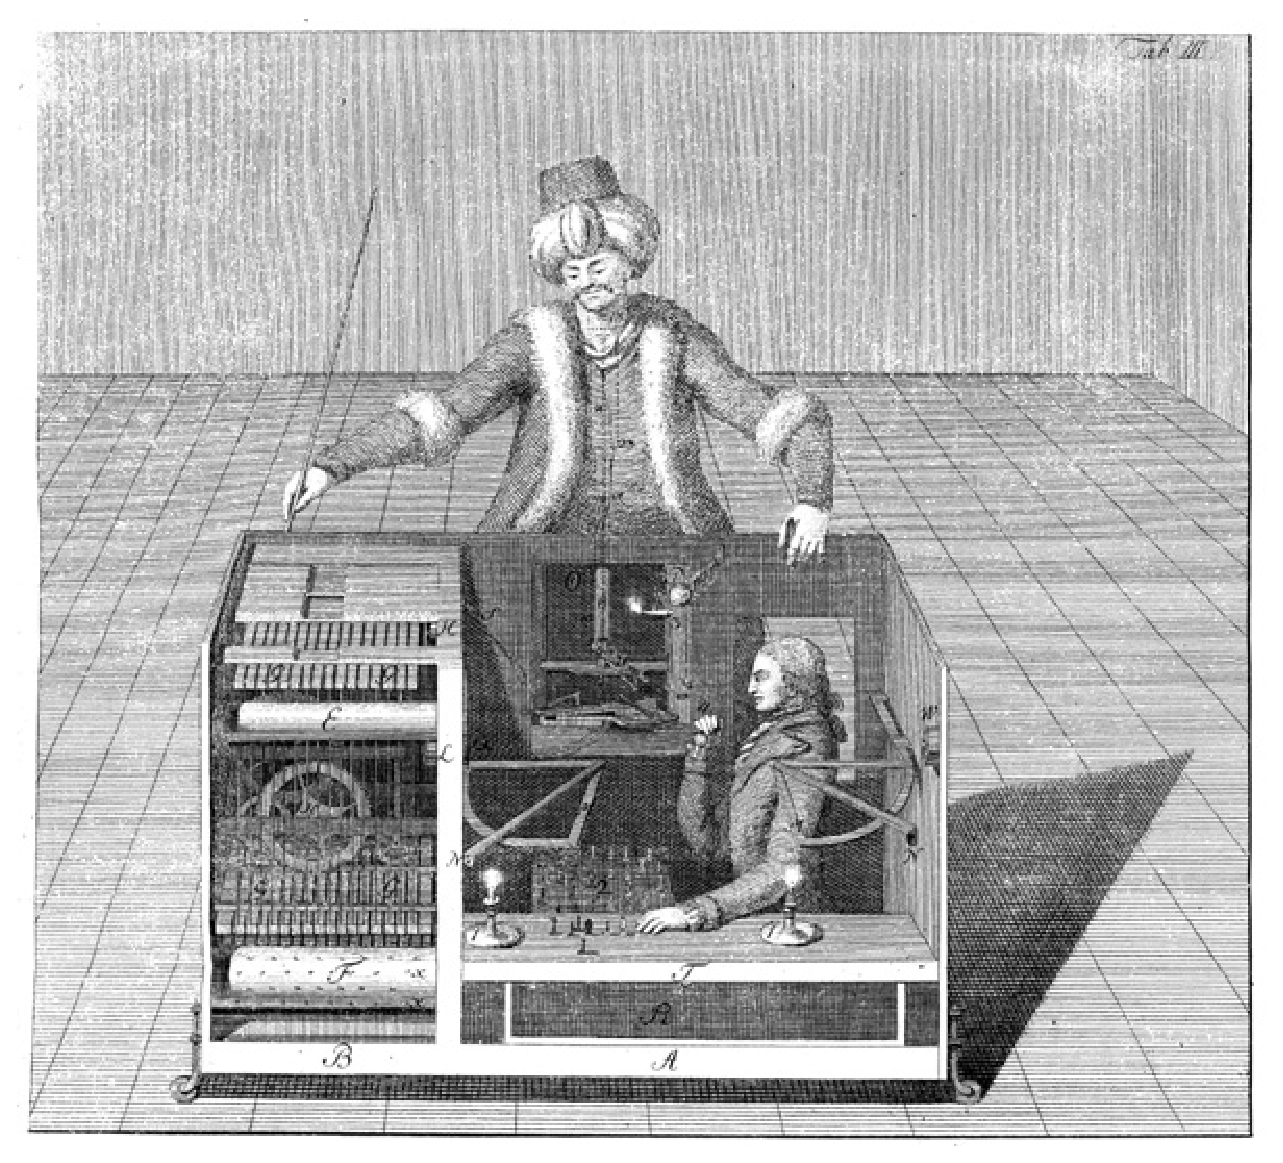
\epsfig{figure=Figures/mfake.eps,height=4in}}
\end{document}
